\documentclass[a4paper]{report}
\usepackage[margin=1.6in]{geometry}

\usepackage[utf8]{inputenc}
\usepackage[T1]{fontenc}
\usepackage{textcomp}
%\usepackage[spanish]{babel}
\usepackage[spanish,es-noshorthands]{babel}
\decimalpoint

\usepackage{csquotes}
\usepackage[sorting=none]{biblatex}
\addbibresource{refs.biblatex}

\usepackage{amsmath, amssymb}
\usepackage{amsthm}
\usepackage{bm}
\usepackage{braket}

\usepackage{graphicx}
\usepackage{subfig}

\usepackage{hyperref}
\hypersetup{
    colorlinks,
    citecolor=red,
    filecolor=black,
    linkcolor=blue,
    urlcolor=black
}

\usepackage{tikz}
\usetikzlibrary{cd}

%\usepackage{layouts}

%\usepackage[marginal]{showlabels}

\DeclareMathOperator{\R}{\mathbb{R}}
\DeclareMathOperator{\Q}{\mathbb{Q}}
\DeclareMathOperator{\C}{\mathbb{C}}
\DeclareMathOperator{\N}{\mathbb{N}}
\DeclareMathOperator{\Z}{\mathbb{Z}}
\DeclareMathOperator{\F}{\mathbb{F}}
\DeclareMathOperator{\E}{\mathbb{E}}

\let\H\relax
\DeclareMathOperator{\H}{\mathcal H}
\DeclareMathOperator{\Sz}{\mathcal S}

\DeclareMathOperator{\dom}{Dom}
\DeclareMathOperator{\prob}{Prob}
\DeclareMathOperator{\id}{id}
\DeclareMathOperator{\Tr}{Tr}
\DeclareMathOperator{\tr}{tr}
\DeclareMathOperator{\Op}{Op}
\DeclareMathOperator{\W}{W}
\DeclareMathOperator{\Fr}{\mathcal{F}\!}
\DeclareMathOperator{\GF}{GF}
\DeclareMathOperator{\GR}{GR}
\DeclareMathOperator{\Sl}{\mathfrak{sl}}
\DeclareMathOperator{\Gal}{Gal}

\newtheorem{definition}{Definición}
\newtheorem{theorem}{Teorema}
\newtheorem{proposition}{Proposición}
\newtheorem{lemma}{Lema}
\newtheorem{corollary}{Corolario}
\newtheorem{example}{Ejemplo}
\newtheorem{axiom}{Postulado}
\newtheorem{remark}{Observación}

\hfuzz=59pt

\begin{document}
  \begin{titlepage}
    \begin{center}
      \vspace{1.0in}

      \huge
      Universidad de Guadalajara\\
      \vspace{0.2cm}
      \large
      Centro Universitario de Ciencias Exactas e Ingenerías\\
      Licenciatura en Matemáticas\\

      \vspace{0.5in}

      
\includegraphics[width=0.3\textwidth]{imgs/udg}
      
      \vspace{0.5in}

      \huge
      \textbf{
        Funciones de Wigner en el Espacio de Fase Discreto
      }

      \large
      \vspace{1.0in}
      
      Alumno: Ernesto Camacho Ramírez \\
      \vspace{0.2cm}
      Asesor: Dr. Andrés García Sandoval \\

      \vfill
           
      \textit{Proyecto integrador}: Estudio de las
      disciplinas fundamentales de la matemática.
     \end{center}
  \end{titlepage}

  \tableofcontents

  \newpage
  \section{Introducción}

  El número de elementos de un conjunto general de
  operadores cuánticos unitarios sobre estados de $n$-qudit
  generalmente crece exponencialmente con $n$. Una excepción
  importante a ésta regla involucra el conjunto de
  operadores de Clifford, que actúan sobre estados
  estabilizadores. Los operadores de Clifford son los
  operadores que normalizan el grupo de Pauli, y los
  estados estabilizadores son los eigenestados simultáneos
  de un subconjunto maximal de operadores de Pauli
  conmutativos. Éstos estados juegan un papel importante
  en la corrección de errores cuánticos \cite{gottesman1998}
  y son cerrados bajo la acción de las compuertas de
  Clifford. La simulación eficiente de dichos sistemas con
  una computadora clásica se demostró con el algoritmo
  tableau de Aaronson y Gottesman \cite{aaronson2004,
  gottesman1998} para qubits ($d=2$). La busqueda de un
  explicación de por qué un algoritmo tan eficiente es
  posible para la simulación de circuitos de Clifford ha
  sido un objeto de mucho estudio \cite{gottesman1999,
  howard2014, mari2012}. El progreso reciente ha sido
  resultado del trabajo de Wooters \cite{wootters1987},
  Eisert \cite{mari2012}, Gross \cite{gross2006} y Emerson
  \cite{howard2014}, quienes han formulado una nueva
  perspectiva basada en los espacios de fase discretos de
  estados y operadores en espacios de Hilbert finitos,
  utilizando funciones discretas de Wigner.  La función de
  Wigner en el caso continuo surge de vincular la mecánica
  cuántica con la mecánica clásica estadística, mediante el
  espacio de fase. Las funciones de Wigner nos dan una
  representación alternativa de estados de sistemas
  cuánticos, por medio de \textit{cuasi-distribuciones}
  sobre el espacio de fase. Éstas funciones no son
  distribuciones probabílisticas verdaderas ya que pueden
  tomar valores negativos, y ésta negatividad ha sido
  vinculada con la no-localidad. La generalización a
  sistemas discretos a tomado distintas formas a traves de
  los años, cada una con ventajas y desventajas. Para una
  clase particular de funciones de Wigner discretas, se ha
  demostrado que los estados estabilizadores son análogos
  discretos a los estados Gaussianos en sistemas continuos
  \cite{gross2006}, en el sentido de que tienen funciones de
  Wigner no-negativas. Por otro lado se ha demostrado
  que los operadores de Clifford son mapeos definidos
  positivos, ésto implica que los circuitos de Clifford son
  simulables eficientemente en computadores clásicas.

  En este trabajo, buscamos construir de una manera
  explícita, a los operadores \textit{puntuales de fase}
  discretos (núcleos de la transformación de Wigner) para
  qubits y qutrits. En particular, desarrollamos la
  construcción \textit{estándar} siguiendo la metodología de
  Gibbons y Wootters \cite{wootters1987}, y como
  contribución del trabajo, buscamos una construcción
  \textit{no estándar} de los núcleos por medio de bases no
  equivalentes (bajo transformaciones unitarias) a las bases
  de la construcción estándar. La motivación para realizar
  éste trabajo es que los núcleos de la construcción no
  estándar preservan las propiedades de la construcción
  estándar por lo tanto pueden ser utilizados para definir
  una función de Wigner. En particular, preservan la
  propiedad tomográfica, la cual permite expresar la función
  de Wigner de cualquier estado como una combinación lineal
  de probabilidades observadas. La inequivalencia de las
  construcciones conduce a la \textit{posibilidad} de
  encontrar estados no estabilizadores con funciones de
  Wigner no-negativas, lo que contrasta con resultados
  previos para el caso discreto \cite{gross2006, galvao2005,
  cormick2006a}.

  \chapter{Preliminares}

  La función de Wigner es una función sobre el espacio de
  fase que nos brinda una representación alternativa de los
  sistemas cuánticos. Dicha función es la parte esencial de
  una formulación completa de la teoría de la mecánica
  cuántica sobre el espacio de fase. Inicialmente solo se
  consideraban sistemas de dimensión infinita en donde las
  variables de posición y de momentum del sistema toman
  valores de $\R^{n}$. Alrededor de los años 80s se hicieron
  múltiples intentos de generalizar el concepto de la
  función de Wigner a sistemas de dimensión finita. Para los
  sistemas continuos resulta que la función de Wigner es
  prácticamente única en el sentido de que posee la
  propiedad tomográfica \cite{ellinas2008}, pero para
  sistemas discretos no hay una función de Wigner única, e
  incluso hay distintas construcciones con distintas
  propiedades.  Esencialmente existen dos versiones básicas,
  una que imita la construcción de la versión continua de
  una manera muy natural y otra construcción que se basa en
  las propiedades que satisface la versión continua. En éste
  trabajo adoptamos la segunda construcción, la cual se debe
  a Wootters. La razón principal para ésta elección es que
  nos brinda una metodología que se puede aplicar para una
  construcción alternativa de la función Wigner.

  Para poder estudiar la función de Wigner discreta es
  necesario presentar la función en el caso continuo. Para
  ésto requerimos un conocimiento básico de la mecánica
  cuántica. A diferencia de la mecánica clásica, la teoría
  cuántica es naturalmente probabilística y sus
  formulaciones matemáticas son bastante distintas. En la
  mecánica clásica, cuando se fija un estado de un sistema
  físico, el valor especificado por un observable (algo se
  puede medir del sistema) está completamente determinado.
  En la mecánica cuántica ésto ya no es cierto, los
  observables solo nos brindan distribuciones de los
  posibles valores. La siguiente sección introduce los
  conceptos básicos de la mecánica cuántica que
  necesitaremos para formular las funciones de Wigner en el
  caso continuo y discreto. El apéndice
  (\ref{sec:classical-phase-space}) puede ser consultado
  para repasar el concepto del espacio de fase en la
  mecánica clásica de manera introductoria. 

  \section{La mecánica cuántica}

  La teoría cuántica ha tomado distintas direcciones despues
  de su concepción en los años viente y existen distintas
  formulaciones matematicamente equivalentes que surgieron
  despues de las teorias iniciales de Schrödinger (mecánica
  de ondas) y de Heisenberg (mecánica matricial).  La más
  común hoy en dia es la formulación en el espacio de
  Hilbert, la cual fue desarrollada de manera rigurosa por
  Von Neumann en 1932.  La segunda formulación más común,
  especialmente en la teoría cuantica de campos, es la
  formulación de la integral de trayectoria de Feynman
  desarrollada en 1948.  Otra formulación, de particular
  interés para nuestro trabajo, es la formulación en el
  espacio de fase, que tiene sus inicios en 1932 por Wigner,
  pero que solo fue desarrollada como una descripción
  completa de la mecánica cuántica despues de la segunda
  guerra mundial. 

  En cualquiera de las formulaciones, la mecánica cuántica
  como toda teoría física, permite el cálculo del
  comportamiento y las propiedades de sistemas físicos. Dado
  un sistema físico, se definen los \textit{observables}
  como las cantidades que podemos medir sobre el sistema,
  por ejemplo la temperatura de algún cuerpo. En la
  formulación de Schrödinger, a los sistemas físicos se le
  asocia un espacio de Hilbert separable. Los observables
  físicos son representados por los operadores auto-adjuntos
  definidos en algún subespacio del espacio de Hilbert. El
  estado de un sistema representa toda la información del
  sistema en algún momento y está dado por operadores
  auto-adjuntos que satisfacen ciertas condiciones
  adicionales. Cuando no hay incertidumbre sobre el estado
  en el que está el sistema, podemos representar el estado
  por un vector del espacio de Hilbert, y decimos que el
  sistema está en un estado puro.

  El ejemplo físico básico es el de una partícula moviendose
  en un espacio Euclideano. El espacio de Hilbert asociado a
  éste sistema generalmente es el espacio de las funciones
  cuadráticamente integrables $L^2(\R^{n})$. Los estados
  puros del sistema son los elementos de éste espacio y el
  operador correspondiente al observable de la posición de
  la partícula es el operador que multiplica una función por
  la coordenada. La mecánica cuántica nos dice que no
  podemos predecir la posición exacta de una partícula en un
  estado arbitrario, lo único que podemos hacer es obtener
  la \textit{probabilidad} de encontrar a la partícula en
  algún subconjunto de $\R^{n}$.  Estadísticamente, nos
  interesa obtener el \textit{valor esperado} de la posición
  de la partícula en un estado en específico, así como el
  valor esperado de otros operadores de interés como lo son
  la energía del sistema, el momentum, el momentum angular,
  entre otros. La mecánica cúantica nos permite estudiar los
  sistemas y sus observables de manera probabilística y
  también nos permite describir su evolución temporal por
  medio de la ecuación de Schrödinger. 
  
  \subsection{Postulados de la mecánica cuántica}

  Comencemos definiendo los conceptos y algunos de los
  postulados que necesitaremos de la mecánica cuántica.
  Existen múltiples versiones de los postulados, dependiendo
  del rigor matemático con el cual se planea trabajar. Para
  ésta sección adaptamos las definiciones del libro de Brian
  Hall \cite{hall2013}.
  \begin{axiom}
    \label{ax:1}
    A cada sistema cúantico le corresponde un espacio de
    Hilbert $\H$. Los estados del sistema son todos los
    operadores lineales $\rho : \H \to \H$,
    definidos-positivos y de traza finita, tales que $\Tr(
    \rho) = 1$.
  \end{axiom}
  Un estado cuántico $\rho$ se dice \textit{puro}, is
  existe un elemento $\psi \in \H$, tal que para todo
  $\alpha \in \H$ se cumple
  \[
    \rho(\alpha)
    = \frac{\braket{\psi | \alpha}}{\braket{\psi | \psi}}
    \psi,
  \] 
  donde $\braket{\cdot|\cdot}$ es el producto interno del
  espacio de Hilbert en cuestion. De ésta manera, cuando
  hablemos de un estado puro, podremos referirnos a un
  elemento $\psi \in \H$, algo que casi siempre sucede en la
  literatura física.

  \begin{axiom}
    \label{ax:2}
    A cada observable físico, $A$, sobre el espacio de fase
    clásico, le corresponde un observable cuántico
    representado por un operador auto-adjunto del espacio de
    Hilbert, 
    \[
      \hat{A} : \mathcal D_{\hat{A}} \to \H.  
    \]
  \end{axiom}
  Los operadores auto-adjuntos representan a los observables
  físicos como por ejemplo la energía, posición, momentum y
  momentum angular. Pero también pueden representar
  observables que no tienen un análogo clásico. Por ejemplo
  pueden representar los grados de libertad de un sistema
  \textit{spin} mediante un espacio de dimensión finita. La
  matemática se vuelve más sencilla en el caso finito ya que
  no se tiene que lidiar con las sutilizas del continuo. Por
  ésta razón, muchos de los tratados sobre la \textit{teoría
  de la medición cuántica} generalmente se hacen en el caso
  finito, evitando las cuestiones delicadas pertinentes de
  la convergencia, cuestiones de acotamiento y del dominio
  del operador, etc.  Muchos problemas surgen del ignorar
  éstos detalles y se pueden tratar rigurosamente con la
  teoría espectral, pero dada la naturaleza de éste trabajo,
  nos podemos dar el lujo de ignorarlos pues nos centramos
  en el estudio de sistemas finitos. 

  El proceso de medición consiste de la prueba o
  manipulación de un sistema físico para obtener un valor
  númerico. En la mecánica cuántica, dichas predicciones son
  probabilísticas de manera natural. A pesar de las
  cuestiones filosóficas que aun no se resuelven
  rotúndamente sobre todo en la cuestión de la medición,
  experimentalmente es un éxito. La prescripción que
  seguiremos para obtener la información probabilística del
  sistema está dada por el postulado de la medición:
  \begin{axiom}
    \label{ax:3}
    Si un sistema cuántico está en un estado descrito por un
    vector unitario $\psi \in \H$, entonces el valor
    esperado de un observable $A$ satisface
    \[
      \braket{\hat A}_\psi
      := \braket{\psi|\hat A \psi},
    \] 
    De manera general, dado un estado $\rho$, el valor
    esperado de un observable $\hat{A}$ está dado por
    \[
      \Tr\left(\hat{A}\rho\right)
      = \Tr\left( \rho\hat{A} \right),
    \]
    donde $\Tr$ es la traza del operador.
  \end{axiom}
  Los valores que pueden tomar los observables cuánticos
  pertenecen al \textit{espectro} del operador. En la
  literatura física es común que se consideren los elementos
  del espectro como los eigenvalores del operador, pero el
  espectro generalmente es mucho más grande. En cuanto al
  postulado de medición, ésto nos dice que a la hora de
  hacer una medición de un observable en un estado cuántico
  $\psi$, mediremos un elemento del espectro y el estado
  colapsa a una `eigenfunción' correspondiente a dicho
  valor. En el caso finito, las cuestiones matemáticas se
  vuelven más fácil porque el espectro de los operadores
  auto-adjuntos \textit{sí} es el conjunto de eigenvalores
  del operador. Por el momento nos enfocamos en sistemas
  cuánticos discretos para poder estudiar un poco más fondo
  el concepto de la medición.

  \section{En dimensión finita}

  El ejemplo clásico es el del \textit{spin} de una
  partícula, la cual toma una cantidad de valores finitos.
  El ejemplo físico más sencillo es el de las partículas de
  spin-$\frac{1}{2}$, en éste caso el spin solo toma dos
  valores, y se dice que la partícula es de $2$-niveles.
  Para una partícula de $d$-niveles, el espacio de Hilbert
  correspondiente es $\H  = \C^{d}$. Para el caso finito,
  adoptaremos por completo a la notación (maquinaria) de P.
  A. M. Dirac, pues es una manera fácil de hacer cálculos y
  de expresar a los operadores de los observables y aquellos
  correspondientes a los estados puros. En ésta notación,
  los estados puros $\psi$ del sistema cuántico, se denotan
  con un \textit{ket}, $\ket \psi$. A cada ket, le
  corresponde un funcional lineal llamado \textit{bra},
  $\bra \psi$, el cual se define por su acción:
  \[
    (\bra \psi)(\ket{\phi})
    := \braket{\psi|\phi}.
  \] 
  Utilizando el bra, para todo estado puro $\ket{\psi}$
  podemos formar un operador de rango uno, que resulta ser
  la proyección $\Pi_\psi$ al subespacio generado por
  $\ket{\psi}$, dicho operador está formado por el producto
  tensorial del dual de $\ket{\psi}$ con $\ket{\psi}$:
  \begin{equation}
    \ket \psi \bra \psi
    := \Pi_\psi
    = \ket \psi \otimes \bra \psi.
  \end{equation} 
  Su acción sobre algun elemento del espacio de Hilbert se
  expresa de manera muy natural utilizando la notación de
  Dirac:
  \[
    \left(\ket \psi \bra \psi\right) \ket \phi
    = \braket{\psi|\phi} \ket \psi.
  \] 
  Dado que los observables son operadores auto-adjuntos, sus
  eigenestados forman una base ortonormal del espacio de
  Hilbert. En particular las proyecciones de cada elemento
  de la base ortonormal son auto-adjuntos. En general los
  operadores auto-adjuntos satisfacen las siguientes
  propiedades:
  \begin{proposition}
    Si $A$ es un operador auto-adjunto entonces:
    \begin{enumerate}
      \item Sus eigenvalores son reales.
      \item Sus eigenestados son ortogonales.
      \item Existe una base ortonormal del espacio de
        Hilbert que consiste de los eigenestados del
        operador (normalizados).
    \end{enumerate}
  \end{proposition}
  %En éste trabajo no trataremos con la dinámica de un
  %sistema cuántico, por lo que no será necesario introducir
  %el concepto de la evolución unitaria de un sistema
  %cuántico.

  \subsection{Medidas proyectivas}

  La idea básica de la teoría de medición consiste en el
  hecho de que podemos elegir \textit{cualquier} base
  ortonormal del espacio de Hilbert $\H$ y observar en que
  estado de la base se encuentra nuestro sistema cuántico.
  Al hacer la medición siempre encontraremos uno de los
  estados de dicha base, y, utilizando el postulado de la
  medición (\ref{ax:3}), podemos calcular la probabilidad de
  observar una de las posibles mediciones. Una medición de
  éste tipo se conoce como \textit{medición de Von Neumann}
  ó medición proyectiva.  Existen otros tipos de mediciones
  que generalizan éste concepto, como las POVMs (medidas de
  operadores positivos), pero la construcción de la función
  de Wigner está basada en las medidas proyectivas así que
  no será necesario estudiar esas alternativas para éste
  trabajo.

  La regla que asigna una probabilidad al evento de observar
  un valor específico de los posibles se conoce como la
  \textit{regla de Born}. Si tenemos un operador
  auto-adjunto, sus eigenvectores y eigenvalores forman un
  conjunto de posibles mediciones. Denotemos por $m$ el
  resultado correspondiente al eigenestado $\ket{\phi_m}$.
  Entonces la regla de Born nos dice que la probabilidad de
  observar a $m$ está dada por la norma cuadrada de la
  proyección del vector $\ket \psi$ hacia el subespacio
  generado por el vector $\ket{\phi_m}$, i.e., si
  $\Pi_{m}$ representa dicha proyección, entonces:
  \begin{equation}
    p(m)
    = \|\Pi_m\ket \psi\|^2
    = \braket{\psi|\Pi_m^{*}\Pi_m|\psi}
    = \braket{\psi|\Pi_m|\psi}.
  \end{equation}
  La última igualdad se sigue de que las proyecciones son
  idempotentes y auto-adjuntos. En otras palabras, la
  probabilidad de obtener $m$ en una medición corresponde al
  valor esperado de la proyección $\Pi_m$ en el estado
  $\ket{\psi}$. Utilizando cualquier base ortonormal
  $\{\ket{\varphi_n}\}$, podemos expresar a la regla de Born
  en términos de la traza para un estado puro $\ket{\psi}$
  de la siguiente manera:
  \begin{align}
    p(m)
    &= \braket{\psi|\Pi_m|\psi} \\
    &= \sum_{n}^{}
    \braket{\psi|\varphi_n}\braket{\varphi_n|\Pi_m|\psi} \\
    &= \sum_{n}^{}
    \braket{\varphi_n|\Pi_m|\psi}\braket{\psi|\varphi_n} \\
    &= \Tr\left( \ket\psi\bra\psi \Pi_m \right).
  \end{align}
  
  Para proyecciones de rango uno, es decir operadores de que
  proyectan a subespacios unidimensionales, es fácil
  observar que la probabilidad de la medición $m$, $p(m)$,
  es igual a los coeficientes de la expansión del estado
  en la base de medición, ya que podemos expresar la
  proyección como $\Pi_m = \ket m \bra m$:
  \begin{align}
    p(m)
    &= \braket{\psi|\Pi_m|\psi} \\
    &= \braket{\psi|m} \braket{m|\psi} \\
    &= \overline{\braket{m|\psi}} \braket{m|\psi} \\
    &= \left|\langle m|\psi \rangle\right|^2.
  \end{align}
  Una \textit{medida proyectiva} es un conjunto de
  proyecciones que proyectan hacia subespacios ortogonales y
  cuya suma es igual al operador identidad. Los
  eigenvectores de operadores auto-adjuntos forman una
  medida proyectiva.  Es evidente que la suma de las
  probabilidades debe ser igual a $1$ para una medida
  proyectiva, ya que la suma de las proyecciones nos da la
  identidad, y los estados cuánticos puros son de norma
  unitaria por el primer postulado:
  \begin{equation}
    \sum_{m}^{} p(m)
    = \sum_{m}^{} \braket{\psi|\Pi_m|\psi}
    = \braket{\psi|\left( \sum_{m}^{} \Pi_m \right)|\psi}
    = \braket{\psi|I|\psi}
    = 1.
  \end{equation}

  Hasta ahorita hemos expuesto los mecanismos de la medición
  para estados puros. Éstos corresponden a la posesión de la
  información completa del sistema, algo generalmente no es
  el caso. Ahora supongamos que no se conoce con certeza en
  que estado está el sistema. Lo único que sabemos es que el
  sistema está preparado en el estado $\ket{\psi_k}$ con
  probabilidad $p_k$ de una colección de posibles estados
  $\{(p_k, \ket{\psi_k})\}$, de tal modo que $\sum_{k}^{}
  p_k = 1$. Con ésto podemos darle un significado al uso de
  operadores para describir estados cuánticos como lo
  hicimos en el primero postulado.
  \begin{definition}
    \label{def:density_operator}
    Si el conjunto $\{(p_k, \ket{\psi_k})\}$ corresponde a
    un estado mixto, entonces definimos al operador de
    densidad como 
    \begin{equation}
      \rho 
      = \sum_{k}^{} p_k \ket{\psi_k}\bra{\psi_k}.
    \end{equation}
  \end{definition}
  \begin{proposition}
    Un operador $\rho$ es el operador de densidad asociado a
    conjunto estadístico $\{(p_k, \ket{\psi_k})\}$ si y solo
    si es auto-adjunto, positivo y de traza unitaria.
  \end{proposition}
  Resulta que la correspondencia entre conjuntos
  estadísticos y operadores de densidad no es única.
  Distintos conjuntos estadísticos nos llevan al mismo
  operador de densidad. Por lo tanto tienen los mismos
  valores esperados para cualquier observable y en efecto
  son indistinguibles. Es por ésto que el operador de
  densidad es la generalización más natural de un estado
  cuántico, en lugar de simplemente los vectores unitarios
  del espacio de Hilbert. Es común confundir el significado
  de la superposición de estados cuánticos y una mezcla de
  estados. Para ganar intuición, podemos considerar el
  ejemplo de una mezcla de dos estados. Ésta mezcla describe
  nuestra \textit{falta de conocimiento}, el sistema
  realmente se encuentra en uno de los dos, solo que no
  sabemos cual es. En cambio, una superposición de estados,
  el sistema \textit{no} se encuentra en uno de los dos
  específicamente, sino que el estado se encuentra en ambos
  a la vez (o en ninguno dependiendo de la filosofía que uno
  adopte).

  Para operadores de densidad, la regla de Born se expresa
  naturalmente como el valor esperado de la proyección
  $\Pi_m$ en el estado $\rho$:
  \begin{equation}
    p(m) = \Tr\left( \rho \Pi_m \right). 
  \end{equation}

  \subsection{Tomografía cuántica y MUBs}

  En la mecánica cuántica, el estado de un sistema cuántico
  no puede ser observado ni puede ser determinado de manera
  experimental. Dado que una sola medición no es suficiente
  para obtener la información necesaria para reconstruir el
  estado cuántico, y dado que la medición afecta el estado,
  se vuelve imposible obtener el resto de la información con
  mediciones subsiguientes \cite{royer1989}. Pero si tenemos
  un conjunto (ensamble) de sistemas \textit{identicamente}
  preparados, la noción de la determinación del estado
  mediante mediciones cobra sentido, ya que se puede, en
  principio, identificar el estado en que se
  \textit{prepara} el sistema cuántico. A ésto se le conoce
  como \textit{tomografía cuántica}.
  
  El uso de las bases mutuamente insesgadas (MUBs) ha sido
  impulsado principalmente por la busqueda de métodos
  óptimos de reconstrucción de estados. Kanat
  \cite{abdukhalikov2015} menciona que las bases mutuamente
  insesgadas fueron estudiadas por primera vez por Schwinger
  en 1960, pero no fueron definidas y ejemplificadas hasta
  1987 por parte de Wootters y Fields \cite{wootters1987}.
  En dicho trabajo Wootters y Fields investigan la
  determinación de estados óptima y llegan a la conclusión
  de que si se puede encontrar un conjunto de $d+1$ bases
  mutuamente insesgadas para un espacio de Hilbert $\H$ de
  dimensión $d$, entonces las mediciones correspondientes a
  esas bases proveen una manera óptima de determinar el
  operador de densidad de un ensamble de estados, en el
  sentido de que el error estadístico es minimizado. Además
  demuestran que la cantidad máxima de MUBs para un sistema
  de dimensión $d$ es precisamente $d+1$ y nos dan una
  manera de cálcular las bases explícitamente.

  La caracteristica de ser mutuamente insesgados es una
  relación entre distintas bases ortogonales del espacio de
  Hilbert, y se define de la siguiente manera.
  \begin{definition}
    Sea $\H = \C^{d}$, decimos que dos bases ortonormales
    $\mathcal B_0 = \{\ket{\psi_i}\}$ y $\mathcal B_1 =
    \{\ket{\phi_j}\}$ son mutuamente insesgadas si
    \begin{equation}
      |\braket{\psi_i|\phi_j}|^2
      = \frac{1}{d},
    \end{equation} 
    para cualesquiera $i$ y $j$.
  \end{definition}
  Dado que tenemos una preferencia por expresar estados
  cuánticos por medio de operadores de densidad, es útil
  notar que podemos expresar ésta noción de ser mutuamente
  insesgado en términos de las proyecciones. Si $\Pi_i$ es el
  operador que proyecta al subespacio generado por
  $\ket{\psi_i}$ y $\Pi_j$ el que proyecta hacia
  $\ket{\phi_j}$, entonces dos bases son mutuamente
  insesgadas si
  \begin{equation}
    \Tr\left( \Pi_i \Pi_j \right) 
    = \frac{1}{d},
  \end{equation}
  para todo $i$ y $j$. El ejemplo más básico es para un
  qubit, donde el sistema cuántico es modelado por el
  espacio $\H = \C^2$.  Un cálculo directo prueba que las
  siguientes bases son mutuamente insesgadas:
  \begin{equation}
    \left\{
      \begin{pmatrix} 1\\0 \end{pmatrix},
      \begin{pmatrix} 0\\1 \end{pmatrix}
    \right\},
    \left\{
      \frac{1}{\sqrt{2}} \begin{pmatrix} 1\\1 \end{pmatrix},
      \frac{1}{\sqrt{2}} \begin{pmatrix} 1\\-1 \end{pmatrix}
    \right\},
    \left\{
      \frac{1}{\sqrt{2}} \begin{pmatrix} 1\\i \end{pmatrix},
      \frac{1}{\sqrt{2}} \begin{pmatrix} 1\\-i \end{pmatrix}
    \right\}.
  \end{equation}
  Éstas son las bases a las que se refiera Kanat, pues
  Schwinger identificó que son los eigenestados de
  operadores que son \textit{complementarios}
  \cite{wootters1989}. Son complementarios en el sentido de
  que la información que obtenemos al medir en un base no
  nos aporta nada en cuanto a los resultados de la medición
  en alguna otra base.

  Hemos mencionado el problema de la determinación de
  estados cuánticos múltiples veces, enseguida hacemos ésto
  más claro. El problema de la determinación de estados, ó
  de tomografía cuántica es el problema de determinar la
  matriz de densidad\footnote{En la literatura física
    generalmente se utilizan los términos matriz de densidad
    y operador de densidad para referirse al mismo objeto,
    nosotros hacemos el ligero incapie en que la matriz de
    densidad es la representación matricial del operador de
  densidad en alguna base.} correspondiente a un ensamble
  de sistemas $d$-dimensionales preparados de manera
  idéntica. Para un sistema de dimensión $d$, la matriz de
  densidad está totalmente determinada por $d^2-1$
  parámetros reales. Una medición en una base de un
  subconjunto del ensamble nos genera solamente $d-1$
  números reales independientes, ya que la regla de Born
  nos dice que su suma debe ser la unidad. Se sigue que
  requerimos \textit{al menos} $d+1$ distintas mediciones
  para recuperar el estado cuántico. Se ha demostrado que si
  uno puede obtener $d+1$ MUBs, entonces las mediciones en
  éstas bases son suficientes para determinar la matriz de
  densidad. No es necesario que las bases sean mutuamente
  insesgadas para recuperar el estado, pero si lo son, nos
  brindan una manera óptima en el siguiente sentido. Como no
  podemos hacer una cantidad infinita de experimentos,
  estamos sujetos al error estadístico que se introduce,
  i.e., no podremos recuperar las probabilidades con
  precisión exacta. Wootters y Fields  establecen ésta
  noción de error estadístico de manera precisa y prueban
  que las mediciones hechas con MUBs son óptimas en el
  sentido de que minimizan el error estadístico. 

  Otro aspecto fundamental de las MUBs para nuestro trabajo,
  es que en general no son únicas, en el sentido de que para
  ciertas dimensiones existen bases que no son unitariamente
  equivalentes.
  \begin{definition}
    Sea $B_k$ la matriz cuyas columnas corresponden a
    elementos de una base $\mathcal B_k$ de un conjunto de
    MUBs $\mathcal B$. Decimos que dos conjuntos de MUBs, 
    \[
      \mathcal B = \{B_0,\ldots,B_k\}
      \quad \text{y} \quad
      \mathcal B' = \{B_0',\ldots, B_k'\},
    \]
    son equivalentes si existe una transformación unitaria
    $U$ de $\C^{d}$ tal que
    \begin{equation}
      \{B_0',\ldots,B_k'\}
      = \{UB_0, \ldots,UB_k\},
    \end{equation}
    donde el orden no se preserva necesariamente.
  \end{definition}
  Calderbank, Cameron, Kantor y Seidel demostraron la
  existencia de varias bases mutuamente insesagados que no
  son equivalentes \cite{kantor2012}, i.e., tales que
  \textit{no} existe una transformación unitaria que
  satisface la definición anterior. Ésto lo hacen a partir
  de la inequivalencia de unas estructuras llamadas
  \textit{coberturas simplécticas}, las cuales veremos en el
  capítulo cuatro.

  Nuestro interés en las MUBs para éste trabajo es que
  surgen de manera natural a la hora de asignar una
  estructura cuántica al espacio de fase discreto para la
  construcción de una función de Wigner discreta. Antes de
  continuar con ese tema es necesario introducir el concepto
  de la función de Wigner. A pesar de que la mayoría de éste
  trabajo se centra en sistemas finitos, nos será útil
  repasar sistemas continuos ó dimensión infinita, ya que la
  función de Wigner originalmente se introdujo para el uso
  en esos sistemas cuánticos.

  \subsection{Sistemas continuos}

  En sistemas continuos, los dos operadores fundamentales de
  la mecánica cuántica son los operadores de posición y de
  momentum. En particular pensemos en el sistema de una
  partícula moviendose sobre la recta real $\R$. El espacio
  de Hilbert es el espacio de las funciones cuadráticamente
  integrables, $L^2(\R)$. Si $\psi \in L^2(\R)$ es un vector
  unitario, entonces $|\psi|^2$ puede ser interpretado como
  la densidad de probabilidad de la posición de la partícula
  en el estado $\psi$, es decir, que la probabilidad de que
  la partícula se encuentre en el subconjunto $B \subset \R$
  es $\int_B |\psi|^2$. A partir de ésto es posible definir
  los operadores de posición y de momentum que satisfacen
  ésta propiedad:
  \begin{definition}
    El operador de posición $\hat X$ se define como
    \[
      \hat X\psi(x) = x\psi(x),
    \] 
    donde $\psi \in L^2(\R)$ es tal que $x\psi \in L^2(\R)$.
  \end{definition}
  Notemos que no existen estados $\psi \in L^2(\R)$ para los
  cuales el operador $\hat X$ toma valores definitivos. Las
  `eigenfunciones' de $\hat X$ nisiquiera son funciones,
  sino \textit{deltas de Dirac} $\delta_{x_0}(x) = \delta(x
  - x_0)$. Éstas se pueden considerar como un conjunto de
  `estados idealizados' y que forman una `base ortonormal
  continua' del espacio de Hilbert en el siguiente sentido:
  \begin{align*}
    \braket{\delta_{x_1}|\delta_{x_2}}
    &= \int \delta(x-x_1)\delta(x-x_2) \, dx
    = \delta(x_1-x_2), \\
    f
    &= \int f(x)\delta_x \, dx
    = \int \braket{f| \delta_x}\delta_x \, dx,
  \end{align*} 
  donde las integrales se interpretan en el sentido de las
  distribuciones de Schwartz. La teoría de distribuciones
  aporta una manera de hacer riguroso los cálculos con los
  deltas de Dirac por medio del triplete de Gel'fand
  \cite{folland1989}, por otro lado, la teoría espectral de
  los operadores auto-adjuntos nos brinda una manera de
  hacer riguroso toda la maquinaria matemática necesaria
  para hacer los cálculos sin recurrir a la distribuciones.
  A pesar de ésto, generalmente se opta por utilizar dicha
  maquinaria sin cuidar el rigor con la finalidad de
  facilitar los cálculos. Dado que éstos detalles no
  aparecen en el caso finito, nosotros no seremos muy
  rigurosos a la hora de introducir a la función de Wigner
  en el caso continuo y generalmente optaremos por usar las
  convenciones físicas.

  Es común trabajar con la \textit{función de onda}
  correspondiente a un estado $\psi$, ésto es una
  representación del estado $\psi$ en términos de la
  posición. La función de onda se define como
  \begin{equation}
    \psi(x)
    = \braket{x| \psi},
  \end{equation} 
  donde el $x \in \R$ del lado izquierdo es un `eigenvalor'
  y del lado derecho es un `eigenestado' del operador de
  posición. Por otro lado, podemos definir el operador que
  corresponde al momentum clásico de la siguiente manera:
  \begin{definition}
    El operador de momentum $\hat P$ se define como
    \[
      \hat P\psi(x) = -i \frac{\partial}{\partial x} \psi,
    \] 
    donde $\psi \in L^2(\R)$ es tal que
  \end{definition}
  El operador de momentum también tiene un espectro continuo
  por lo cual es necesario introducir estados generalizados
  para poder hacer cálculos. Además, de manera análoga al
  operador de posición, podemos expresar un estado $\psi$ en
  términos del momentum mediante
  \begin{equation}
    \psi(p)
    = \braket{p| \psi},
  \end{equation} 
  donde de nuevo $p$ representa los eigenestados de $\hat
  P$. Notemos que las funciones $\psi(x)$ y $\psi(p)$ son
  dos representaciones del \textit{mismo} estado $\psi$.  La
  transformación de Fourier conecta a la función de posición
  $\psi(x)$ con la del momentum $\psi(p)$ de la siguente
  manera:
  \begin{equation}
    \psi(x)
    = \frac{1}{\sqrt{2\pi\hbar}} \int_{\R} \psi(p)e^{ixp /
    \hbar} \, dp,
  \end{equation} 
  donde $\hbar$ es la constante de Planck. Ésta relación es
  una de las razones por la cual se les llama a las
  \textit{variables} de posición y momentum,
  \textit{variables conjugadas}.

  Los estados mixtos se expresan de una manera análoga al
  caso finito. Definimos un estado mixto como un conjunto de
  pares $\{(\lambda_j,\psi_j)\}_{j \in \N}$ donde cada
  $\psi_j \in L^2(\R^{n})$ es un estado puro y $0 \leq
  \lambda_j \leq 1$ es una probabilidad clásica, es decir,
  $\sum_j \lambda_j = 1$.
  \begin{definition}
    Un estado cuántico es el conjunto de pares $(\lambda_j,
    \psi_j) \in [0,1] \times L^2(\R^{n})$, indexado por un
    conjunto discreto $F$ donde $\|\psi_j\|_{L^2(\R^{n})} =
    1$ para todo $j \in F$ y $\sum_{j \in F} \lambda_j = 1$.
    El operador lineal $\hat{\rho}$ sobre $L^2(\R^{n})$
    definido por
    \begin{equation}
      \hat{\rho} \psi
      = \sum_{j \in F}^{} \lambda_j \Pi_{\psi_j} \psi
      = \sum_{j \in F}^{} \lambda_j \braket{\psi| \psi_j}
      \psi_j,
    \end{equation}
    es el operador de densidad asociado al estado. 
  \end{definition}
  El operador de densidad definido de ésta manera es
  auto-adjunto, semi-definido positivo, y es de clase de
  traza con $\Tr(\hat{\rho}) = 1$, por lo tanto cumple con
  el primer postulado de la mecánica cuántica. El espectro
  de un operador de densidad $\hat{\rho}$ sobre
  $L^2(\R^{n})$ es discreto y consiste de números no
  negativos tales que $\lambda_1 \geq \lambda_2 \geq \ldots
  \geq 0$, y $\lim_{j \to \infty} \lambda_j = 0$ (en el caso
  en que $F$ es infinito).

  El postulado de la medición nos dice que podemos calcular
  el valor esperado de un observable cuántico $A$, en un
  estado cuántico $\rho$ de la siguiente manera:
  \begin{equation}
    \langle \hat A \rangle = \Tr(\hat A \rho).
  \end{equation}
  También podemos calcular las probabilidades de observar un
  valor específico de una medición de un observable, éstos
  valores son elementos del espectro del observable en
  cuestión.  Como mencionamos antes, el espectro del un
  observable generalmente es más grande que su conjunto de
  eigenestados. Aún así, podemos trabajar con la idea de
  eigenestados generalizados para poder hacer los cálculos
  de manera análoga como lo hicimos en el caso finito. De
  hecho la función de onda en la representación de la
  posición nos da precisamente la probabilidad de medir la
  posición en un punto $x$ para un estado que modela la
  posición de una partícula. Sucede lo mismo con la función
  de onda en representación del momentum.
  
  La no conmutatividad de los operadores de posición y de
  momentum tiene consecuencias profundas en la teoría de la
  medición.  El principio de incertidumbre nos dice que no
  podemos medir de manera simultánea la posición y momentum
  de una partícula con precisión (ni siquiera en teoría).
  Del repaso de la mecánica clásica en el apéndice
  (\ref{sec:classical-phase-space}), sabemos
  que mediante el uso del espacio de fase, podemos
  representar a los estados de un sistema físico por puntos
  en el plano $\R^2$. En la mecánica clásica sí es posible,
  en teoría, medir la posición y el momentum de una
  partícula en cualquier momento. Por lo tanto tiene sentido
  representar al estado de un sistema como un punto en el
  plano. La evolución temporal del sistema forma
  trayectorias en el plano de acuerdo a las leyes de
  movimiento. En el caso cuántico el principio de
  incertidumbre no nos permite localizar el estado en un
  espacio de fase. Pero, no todo está perdido, hay maneras
  de vincular éstos dos conceptos por medio de las
  cuasi-distribuciones, y en particular la función de
  Wigner.

  \chapter{Función de Wigner}

  \section{Mecánica cuántica en el espacio de fase}

  En éste capítulo introducimos el concepto de la función de
  Wigner y la formulación de la mecánica cuántica en el
  espacio de fase. El principio de la incertidumbre hace que
  la noción de un espacio de fase análogo al de la
  mecánica clásica, sea problemático para la teoría
  cuántica. Ésto se debe a que la posición y el momentum de
  una partícula no se pueden medir de manera simultánea.
  Aún así existen funciones que se \textit{asemejan} a
  distribuciones probabilísticas sobre el espacio de fase,
  llamadas funciones de distribución cuasi-probabilísticas,
  las cuales son útiles de manera práctica, además de
  vincular de cierta manera a la mecánica clásica y la
  cuántica. Ésto sucede porque dichas cuasi-distribuciones
  nos permiten calcular los valores esperados de los
  operadores cuánticos de manera muy similar a los promedios
  clásicos de la mecánica estadística. La primera y la que
  estudiamos en éste trabajo es la función de Wigner.

  La función de Wigner tiene una larga historia que inicia
  con un artículo publicado por Eugene P. Wigner en 1932
  \cite{wigner1932} sobre correcciones cuánticas del
  equilibrio termodinámico. La idea principal de Wigner fue
  introducir una cuasi-distribución que le permite calcular
  valores esperados cuánticos de una manera análoga a los
  valores esperados de la mecánica estadística. Para el caso
  de una función $\psi$ cuadráticamente integrable, la
  expresión que expuso Wigner originalmente (para un sistema
  de una dimensión) es:
  \begin{equation}
    \label{eqn:wigners_original}
    W_\psi(x,p)
    = \frac{1}{\hbar \pi} \int_{\R}
    \overline{\psi}(x+y)\psi(x-y) e^{\frac{2i}{\hbar}py} \,
    dy.
  \end{equation}
  En el caso de un estado cuántico puro, la función
  $W_\psi(x,p)$ representa al estado $\psi$ de manera
  análoga a una densidad probabilística sobre el espacio de
  fase. Wigner partió de la mecánica estadística clásica, en
  donde la evolución del sistema puede ser estudiado de
  manera probabilística mediante la ecuación de Liouville,
  la cual nos brinda una distribución sobre el espacio de
  fase.  Su idea fue construir una distribución que nos
  permita hacer los mismos cálculos probabilísticos de la
  mecánica cuántica que se pueden hacer con la formulación
  en el espacio de Hilbert.

  Unos años antes de la publicación de Wigner, Hermann Weyl
  formuló una manera de mapear observables clásicos a
  observables cuánticos, lo cual se conoce como la
  \textit{cuantización de Weyl} \cite{degosson2021}. Debido
  a la no conmutatividad de los operadores canónicos $\hat
  X$ y $\hat P$, la cuantización de un observable clásico no
  es única y es necesario introducir un orden específico, la
  cuantización de Weyl es un caso específico.  Weyl utilizó
  la transformación de Fourier para producir operadores
  correspondientes a ciertas funciones de $x$ y $p$ en el
  espacio de fase que satisfacen algunas condiciones de
  regularidad. Existe una relación directa entre los mapeos
  de Weyl y de Wigner y nos es útil introducir el mapeo de
  Weyl primero.

  Utilizando las transformaciones de Wigner y de Weyl,
  Enrique Moyal y Groenewold formularon de manera
  independiente, una descripción \textit{completa} de la
  mecánica cuántica en el espacio de fase
  \cite{curtright2012}. Ésta tercera formulación de la
  mecánica cuántica, ha sido muy útil en muchas ramas de la
  física, particularmente en la óptica cuántica
  \cite{zachos2005}. En éste trabajo no daremos un resumen
  de ésta formulación, en caso de que el lector esté
  interesado, le invitamos a consultar los trabajos de Moyal
  \cite{moyal1949} y de Groenwold \cite{groenewold}.

  %El trabajo de Groenewold (en forma de su tésis de 1946)
  %reconoció que el mapeo de Weyl es realmente una
  %transformación invertible, y \textit{no} solo una regla de
  %cuantización \cite{todorov2012}. Por otro lado Moyal
  %desarrolló sus ideas sobre la naturaleza estadística de la
  %mecánica cuántica, y en su formulación se introduce un
  %producto en el espacio de fase correspondiente al producto
  %de operadores en el espacio de Hilbert, tal producto se le
  %conoce como el producto-$\star$ ó producto de Moyal.

  \section{La transformación de Wigner-Weyl}

  En ésta sección vamos definir la transformación de Wigner
  para estados puros, los cuales serán elementos de
  $L^2(\R)$, para posteriormente definir la función de
  Wigner de un estado cuántico arbitrario. Para iniciar,
  introducimos el concepto de la cuantización de Weyl porque
  de ésta forma surgen de manera muy natural varios de los
  objetos que aparecen en las definiciones de la función de
  Wigner, independientemente si el sistema es continuo o
  discreto.

  Recordemos la motivación de la sección anterior.
  Consideremos un conjunto de partículas que se mueven en un
  espacio $\R^{n}$. La ecuación de Liouville rige la
  evolución temporal de una función de distribución en el
  espacio de fase del conjunto de partículas. La solución de
  dicha ecuación nos brinda una densidad probabilística y
  dado un observable clásico $A : \R^{2n} \to \R$, que
  depende de la posición $x$ y del momentum $p$ de una
  partícula, podemos calcular el valor esperado del
  observable como una integral sobre el espacio de fase
  \begin{equation}
    \mathbb E[A]
    = \iint A(x,p) F(x,p) \, dx \, dp,
  \end{equation}
  donde $F$ es la densidad de probabilidad de Liouville. La
  densidad $F$ contiene toda la información probabilística
  del \textit{conjunto} de partículas, es decir del sistema.
  La intención es poder calcular valores esperados de
  observables cuánticos de manera análoga, es decir,
  mediante una integración en el espacio de fase, en donde
  la densidad que obtenemos representa a algún estado
  cuántico:
  \begin{equation}
    \Tr\left(\hat{\rho} \hat{A}\right)
    = \iint A(x,p)W(x,p) \, dx \, dp,
  \end{equation}
  La función $W : \R^{2n} \to \R$ que actúa como una
  distribución probabilística será precisamente la
  transformación de Wigner de un estado cuántico.
  Desafortunadamente no es una distribución verdadera, pues
  puede tomar valores negativos (de aquí proviene el nombre
  de \textit{cuasi}-distribución). Sin embargo, nos permite
  calcular los valores esperados de los operadores cuánticos
  y otras cantidades probabilísticas como las densidades de
  la posición y momentum de la partícula, dándonos una
  representación de nuestro estado cuántico completo pero
  distinto.

  Notemos que la definición (\ref{eqn:wigners_original}) es
  una transformación integral de una función $\psi \in
  L^2(\R^{n})$. Para poder definir la transformación de un
  estado cuántico $\hat{\rho}$, tendremos que tomar algunos
  pasos previos. En particular, primero introducimos el
  concepto de \textit{cuantización}, lo cual es un proceso
  inverso que nos permite pasar de un observable clásico
  definido en el espacio de fase a un operador cuántico
  definido en el espacio de Hilbert correspondiente.

  \subsection{La transformación de Weyl}

  El problema de la cuantización consiste en encontrar una
  correspondencia entre funciones sobre el espacio de fase
  $\R^{2n}$ y operadores auto-adjuntos sobre $L^2(\R^{n})$,
  tales que las propiedades de los observables clásicos se
  reflejen lo más posible en sus correspondientes operadores
  cuánticos, en una manera consistente con la interpretación
  probabilística de la mecánica cuántica.  Dada la no
  conmutatividad de los operadores de posición y de
  momentum, no hay una correspondencia única, por lo tanto
  se restringe el mapeo de una manera ad-hoc, buscando
  satisfacer ciertas propiedades razonables. Por ejemplo es
  deseable que las funciones coordenadas de posición y de
  momentum $x_j$ y $p_j$ correspondan a los operadores
  $\hat{X}_j$ y $\hat{P}_j$, así como el operador
  correspondiente a la función constante $1$ debe ser el
  operador identidad, entre otros.  A pesar de que no hay un
  manera única de cuantizar observables clásicos, existe una
  que es más \textit{natural}, conocida como la cuantización
  de Weyl. 

  La idea de la cuantización de Weyl, es la siguiente:
  consideramos un observable clásico $A : \R^{2n} \to \R$,
  comunmente llamado \textit{símbolo} en el análisis
  armónico y en la óptica cuántica. Lo podemos expresar
  mediante la transformación de Fourier inversa:
  \begin{equation}
    A(x,p)
    = \frac{1}{(2\pi\hbar)^{n}} \int_{\R^{2n}} \Fr A(\xi,
    \eta) e^{\frac{i}{\hbar} \left( \xi x + \eta p\right) }
    \, d\xi \, d\eta,
  \end{equation}
  donde $\Fr A$ es la transformada de Fourier de $A$.
  Enseguida reemplazamos de manera \textit{formal} a las
  variables $x$ y $p$ por los operadores $\hat{X}$ y
  $\hat{P}$\footnote{Ésto corresponde con el orden simétrico
    de Weyl.}, para obtener al operador $\hat{A}$
  correspondiente:
  \begin{equation}
    \label{eqn:weyl_quant_1}
    \hat{A}(\hat{X},\hat{P})
    = \frac{1}{(2\pi\hbar)^{n}} \int_{\R^{2n}} \Fr
    A(\xi,\eta) e^{\frac{i}{\hbar} \left( \xi \hat{X} + \eta
    \hat{P}\right) } \, d\xi \, d\eta.
  \end{equation}
  Para darle un sentido riguroso a la integral es necesario
  pedir ciertas condiciones de regularidad a la función $A$.
  En la literatura matemática generalmente se comienza por
  definir la transformación de Weyl sobre el espacio de las
  funciones rápidamente decrecientes $\Sz(\R^{2n}) \subset
  L^2(\R^{2n})$ y luego se extiende a las funciones
  cuadraticamente integrables y por dualidad a las
  distribuciones templadas $\Sz'(\R^{2n})$. Evitaremos
  hablar de éstos detalles importantes para no extender el
  tema incesesariamente. El operador exponencial que
  aparece en el integrando de (\ref{eqn:weyl_quant_1}) se
  conoce como el operador característico de Moyal (ó
  operador característico de Weyl).
  \begin{definition}
    El operador $\hat{M}(\xi, \eta) : L^2(\R^{n}) \to
    L^2(\R^{n})$ definido como
    \begin{equation*}
      \hat{M}(\xi,\eta)
      = e^{\frac{i}{\hbar} \left( \xi \hat{X} + \eta \hat{P}
      \right) },
      %= e^{-\frac{i}{2\hbar} \xi \eta} e^{\frac{i}{\hbar}
      %\eta \hat{P}} e^{\frac{i}{\hbar} \xi \hat{X}}
      %= e^{\frac{i}{2\hbar} \xi \eta} e^{\frac{i}{\hbar}
      %\xi \hat{X}} e^{\frac{i}{\hbar} \eta \hat{P}},
    \end{equation*} 
    se conoce como el operador característico de Moyal
    (entre otros nombres). Actúa sobre alguna función $\psi
    \in L^2(\R^{n})$ de la siguiente manera:
    \begin{equation}
      \hat{M}(\xi,\eta)\psi(x)
      = e^{\frac{i}{2\hbar} \xi\eta} e^{\frac{i}{\hbar} \xi
      x} \psi(x + \eta).
    \end{equation}
  \end{definition}
  Utilizando la definición del operador $\hat{M}(\xi,\eta)$,
  podemos definir de manera operacional a la transformación
  de Weyl sobre en subespacio apropiado de $L^2(\R^{n})$.
  \begin{definition}
    Sea $A \in \Sz(\R^{2n})$. El operador de Weyl, $\hat{A}
    = \Op_W(A)$ del símbolo $A$ se define para un $\psi \in
    \Sz(\R^{n})$ apropiado como
    \begin{equation}
      \label{eqn:weyl_quant_2}
      \hat{A}\psi(x)
      = \frac{1}{(2\pi\hbar)^{n}}
      \int_{\R^{2n}} \Fr A(\xi,\eta) \hat{M}(\xi,\eta)
      \psi(x) \, d\xi \, d\eta.
    \end{equation}
  \end{definition}
  Es más común expresar a la transformación de Weyl en
  términos del símbolo $A$ directamente, sin recurrir a la
  transformada de Fourier. Utilizando la definición de
  $\Fr$, de manera formal tenemos:
  \begin{align*}
    \Op_W(A)
    &= \frac{1}{(2\pi\hbar)^{n}} \int_{\R^{2n}} \Fr
    A(\xi,\eta)\hat{M}(\xi,\eta) \, d\xi \, d\eta \\
    &= \frac{1}{(2\pi\hbar)^{n}} \int_{\R^{2n}} \left(
    \int_{\R^{2n}} A(x,p)e^{-i(\xi x + \eta p)} \, dx \, dp
    \right) \hat{M}(\xi,\eta) d\xi \, d\eta \\
    &= \frac{1}{(2\pi\hbar)^{n}} \int_{\R^{2n}} A(x,p)
    \left( \int_{\R^{2n}} e^{-i(\xi x + \eta p)}
    \hat{M}(\xi,\eta) \, d\xi \, d\eta \right) \, dx \, dp
    \\
    &= \frac{1}{(2\pi\hbar)^{n}} \int_{\R^{2n}} A(x,p)
    \hat \Delta(x,p) \, dx \, dp.
  \end{align*} 
  El la literatura matemática, el operador $\hat
  \Delta(x,p)$ se conoce como el operador de Grossmann-Royer
  y generalmente se denota $\hat{R}(x,p)$. En la literatura
  física comunmente es llamado el operador puntual de
  cuantización o del espacio de fase, ó el núcleo de la
  transformación de Wigner. Formalmente se puede ver como la
  transformada de Fourier del operador característico de
  Weyl $\hat{M}(\xi,\eta)$:
  \begin{equation}
    \label{eqn:phase_point_operator}
    \hat \Delta(x,p)
    = \int_{\R^{2n}} e^{-i(\xi x + \eta p)}
    \hat{M}(\xi,\eta) \, d\xi \, d\eta.
  \end{equation}
  Resulta que el mismo operador puntual puede ser utilizado
  para definir la transformación de Wigner, vinculando de
  manera muy natural a dicha transformación con la
  transformación de Weyl. Hemos presentado la idea de la
  cuantización de Weyl para motivar la introducción del
  operador puntual $\hat \Delta$, pero existe otra forma de
  expresar a los operadores puntuales $\Delta(x,p)$
  particularmente iluminadora para nuestros objetivos, por
  medio de los operadores de Heisenberg-Weyl, conocidos
  también como los operadores de desplazamiento. Despues de
  reformular a los operadores puntuales en términos de los
  operadores de desplazamiento, podremos definir la
  transformación de Wigner de un estado $\psi$, en una forma
  que se preservará a la hora de pasar al caso discreto.

  \subsection{Los operadores puntuales del espacio de fase}

  Los operadores de Heisenberg-Weyl son muy estudiados en la
  mecánica cuántica, pues son operadores unitarios sobre
  $L^2(\R^{n})$ que pueden ser utilizados para definir al
  grupo de Heisenberg y son una representación del grupo de
  Galilei, las cuales corresponden a traslaciones en el
  espacio de fase \cite{degosson2011}.
  \begin{definition}
    El operador de Heisenberg-Weyl $\hat{D}(\xi,\eta)$ se
    define como
    \begin{equation}
      \hat{D}(\xi,\eta)\psi(x)
      = e^{\frac{i}{\hbar} (\eta x - \frac{1}{2} \eta
      \xi)}\psi(x - \xi).
    \end{equation} 
    Equivalentemente se puede expresar como
    \begin{equation}
      \hat{D}(\xi,\eta)\psi(x)
      = e^{\frac{i}{\hbar} \sigma((\xi,\eta),
      (\hat{x},\hat{p}))}\psi(x),
    \end{equation} 
    donde $\sigma((x,p),(x',p')) = p \cdot x' - p' \cdot x$,
    es una forma simpléctica en el espacio de fase.
  \end{definition}
  \begin{proposition}
    \label{prop:HW-ops-props}
    Los operadores de desplazamiento satisfacen las
    siguientes propiedades. Para todo $\psi,\phi \in
    L^2(\R^{n})$ y $z_0,z_1 \in \R^{2n}$, los operadores
    $\hat D(z_0)$ son:
    \begin{enumerate}
      \item Lineales.
        \begin{equation}
          \hat D(z_0)(\lambda \psi + \mu \phi)
          = \lambda \hat D(z_0) \psi + \mu \hat D(z_0)\phi,
          \quad
          \lambda, \mu \in \C.
        \end{equation}
      \item Unitarios.
        \begin{equation}
          \hat D(z_0)^{-1}
          = \hat D(-z_0)
          = \hat D(z_0)^{*}.
        \end{equation}
      \item Satisfacen la relación de conmutatividad:
        \begin{equation}
          \hat{D}(z_0)\hat{D}(z_1)
          = e^{\frac{i}{\hbar} \sigma(z_0,z_1)}
          \hat{D}(z_1)\hat{D}(z_0).
        \end{equation}
      \item Satisfacen la relación de composición:
        \begin{equation}
          \hat D(z_0+z_1)
          = e^{-\frac{i}{2\hbar} \sigma(z_0,z_1)}\hat D(z_0)
          \hat D(z_1).
        \end{equation}
    \end{enumerate}
  \end{proposition}
  Una versión análoga de la proposición
  (\ref{prop:HW-ops-props}) volverá a aperecer cuando
  pasemos a un espacio discreto. Utilizando a los operadores
  de desplazamiento, ahora definimos el operador de
  \textit{Grossmann-Royer}, actuando sobre un operador de
  \textit{paridad} $\hat \Delta(0,0)$ bajo la conjugación de
  un operador de desplazamiento.
  \begin{definition}
    El operador de Grossmann-Royer $\hat{\Delta}(\xi,\eta)$
    es el operador 
    \begin{equation}
      \hat{\Delta}(\xi,\eta) : \Sz(\R^{n}) \to \Sz(\R^{n})
    \end{equation} 
    definido por las formulas 
    \begin{equation}
      \hat{\Delta}(0,0)\psi(x)
      = \psi(-x),
    \end{equation}
    y
    \begin{equation}
      \hat{\Delta}(\xi,\eta)
      = \hat{D}(\xi,\eta) \hat{\Delta}(0,0)
      \hat{D}(\xi,\eta)^{-1},
    \end{equation} 
    donde $\hat D$ es el operador de Heisenberg-Weyl. El
    operador de Grossmann-Royer es unitario y es una
    involución en el espacio de Schwartz. Su acción sobre
    cualquier función $\psi : \R^{n} \to \C$ está dado por
    \begin{equation}
      \hat{\Delta}(\xi,\eta)\psi(x)
      = e^{\frac{2i}{\hbar} \eta (x - \xi)}\psi(2\xi - x).
    \end{equation} 
  \end{definition}
  Elegimos la notación $\hat \Delta$ porque los operadores
  de Grossmann-Royer son precisamente los operadores
  puntuales definidos en la sección anterior. El uso de los
  operadores puntuales nos dará una expresión bastante
  sencilla de la función de Wigner de un estado cuántico, y
  además, muchas de las propiedades interesantes de la
  función de Wigner se heredan de las siguientes propiedades
  de los operadores puntuales.
  \begin{proposition}
    Para todo $\psi,\phi \in L^2(\R^{n})$ y $z_0,z_1 \in
    \R^{2n}$, los operadores puntuales $\hat \Delta(z_0)$
    son:
    \begin{enumerate}
      \item Lineales.
      \item Unitarios.
      \item Satisfacen la relación de composición:
        \begin{equation}
          \hat\Delta(z_0)\hat\Delta(z_1)
          = e^{-\frac{2i}{\hbar} \sigma(z_0,z_1)}
          \hat\Delta(2(z_0-z_1)).
        \end{equation}
    \end{enumerate}
  \end{proposition}
  %Como habíamos comentado, con los operadores puntuales
  %podemos definir el operador de Weyl de manera operacional
  %y en términos del símbolo $A$ directamente:
  %\begin{definition}
  %  Sea $A \in \Sz(\R^{2n})$. El operador de Weyl $\hat{A} =
  %  \Op_W(A)$ está dado para todo $\psi \in \Sz(\R^{n})$ 
  %  como
  %  \begin{equation}
  %    \left( \hat{A}\psi \right)(x)
  %    = \frac{1}{(\pi\hbar)^{n}} \int_{\R^{2n}}
  %    A(\xi,\eta)\hat{\Delta}(\xi,\eta)\psi(x) \, d\xi \,
  %    d\eta.
  %  \end{equation}
  %\end{definition}

  Para ciertos operadores sobre $\H$, es posible invertir la
  transformación de Weyl, un ejemplo del proceso que se
  conoce como \textit{decuantización}. De manera precisa,
  para un operador que admite una representación integral,
  podemos construir un símbolo que es integrable en el
  espacio de fase. Al símbolo obtenido a partir del operador
  de Weyl se conoce como símbolo de Weyl. Ésto nos dice que
  existe una correspondencia entre los símbolos
  cuadracticamente integrables sobre el espacio de fase y
  una clase de operadores acotados de $L^2(\R^{n})$
  \cite{degosson2016}.  Gosson demuestra en partícular, que
  la transformación de Weyl de una función cuadraticamente
  integrable corresponde a un operador Hilbert-Schmidt.
  \begin{definition}
    Un operador de Hilbert-Schmidt es un operador acotado
    $\hat A : \H \to \H$ que tiene una norma de
    Hilbert-Schmidt finita. La norma de Hilbert-Schmidt se
    define como:
    \begin{equation}
      \|\hat A\|^2_{HS}
      = \sum_{i \in I}^{} \|\hat A e_i\|^2_{\H},
    \end{equation}
    donde $\{ e_i : i \in I\}$ es un base ortonormal del
    espacio de Hilbert $\H$. En dimensión finita, la norma
    de Hilbert-Schmidt es idéntica a la norma de Frobenius.
  \end{definition}
  Los operadores de densidad son un ejemplo de operadores
  Hilbert-Schmidt por lo tanto pueden ser transformados a un
  símbolo en el espacio de fase. El proceso de la
  decuantización comunmente se realiza (al menos de manera
  formal) a través de la siguiente fórmula para un operador
  de Weyl
  $\Op_W(A)$:
  \begin{equation}
    A(x,p)
    = \Tr\left( \Delta(x,p) \Op_W(A) \right).
  \end{equation} 
  Ésta expresión solo tiene sentido riguroso de manera obvia
  cuando $\Op_W(A)$ tiene traza finita, entre otros
  requerimientos. De nuevo los operadores de densidad
  satisfacen los requisitos, por lo que se puede utilizar
  dicha fórmula para obtener el símbolo correspondiente.
  Resulta que para un estado cuántico, el símbolo que se
  obtiene de ésta manera es precisamente la función de
  Wigner.

  Resumiendo ésta sección, hemos introducido a los
  operadores puntuales por medio de la cuantización de Weyl,
  y en el camino hemos definido a los operadores de
  desplazamiento.  En la siguiente sección por fin definimos
  la función de Wigner en la manera en que se usará en el
  resto del trabajo.

  %En resumen hemos mostrado una manera de cuantizar
  %observables clásicos, que brinda operadores cuánticos que
  %satisfacen varias propiedades útiles, por ejemplo no es
  %dificil probar que dicha transformación nos brinda los
  %operadores correctos correspondientes a las funciones
  %coordenadas
  %$x_j$ y $p_j$:
  %\begin{equation}
  %  \Op_W(x_j)\psi = x_j\psi,
  %  \quad
  %  \Op_W(p_j)\psi = -i\hbar \partial_{x_j}\psi.
  %\end{equation}
  %Con la transformación de Weyl definida junto con la
  %introducción de los operadores de desplazamientos y los
  %puntuales, pasamos a definir la función de Wigner, la cual
  %coincide con la decuantización de operadores de Weyl.

  \section{La transformación de Wigner}

  Lo que sigue está basado principalmente en los libros de
  Gosson \cite{gosson2017} y de Folland \cite{folland1989},
  quienes introducen la función de Wigner de manera general,
  en el contexto del análisis armónico. Nosotros adaptamos
  el formalismo que ellos emplean en el contexto de la
  mecánica cuántica.
  \begin{definition}
    La transformación de Wigner es una transformación
    integral
    \begin{equation}
      W : L^2(\R^{n}) \to L^2(\R^{2n}),
    \end{equation}
    definida como
    \begin{equation}
      \label{eqn:cross_wigner_transform}
      W(\psi)(x,p)
      = (2\pi\hbar)^{-n} \int_{\R^{n}} e^{-\frac{i}{\hbar} p
      \cdot y} \psi(x + \tfrac{1}{2}y) \overline{\psi(x -
      \tfrac{1}{2}y)} \, dy,
    \end{equation}
    para $\psi \in L^2(\R^{n})$ y $x,p \in \R^{n}$.  
  \end{definition} 
  Denotaremos a la \textit{función de Wigner} de una función
  $\psi$ por el símbolo $W_\psi$. Utilizando los operadores
  puntuales definidos en la sección anterior, se puede
  demostrar fácilmente que la expresión
  (\ref{eqn:cross_wigner_transform}) es equivalente a la
  siguiente expresión.
  \begin{definition}
    Sea $\psi \in \Sz(\R^{n})$ y $\hat\Delta(x,p)$ el
    operador puntual correspondiente al punto $(x,p)$ del
    espacio de fase. La transformación de Wigner $W : \psi
    \mapsto W_\psi$ se puede definir como
    \begin{equation}
      \label{eqn:def_wigner}
      W(\psi)(x,p)
      = \frac{1}{(\pi\hbar)^{n}} \braket{\psi|
      \hat{\Delta}(x,p)\psi}.
    \end{equation}
  \end{definition}
  La transformación de Wigner satisface varias propiedades
  interesantes, por ejemplo, para $\psi \in L^2(\R^{n})$, es
  real valuada, acotada y continua. Las demostraciones se
  pueden encontrar en el libro de Gosson \cite{degosson2016}.
  \begin{proposition}
    Si $\psi \in L^2(\R^{n})$, entonces $W_\psi =
    \overline{W_\psi}$, por lo tanto $W_\psi$ es
    real-valuada. 
  \end{proposition}
  \begin{proposition}
    Sean $\psi \in L^2(\R^{n})$ y supongamos que su función
    de Wigner es absolutamente integrable, i.e., $W_\psi \in
    L^{1}(\R^{2n})$. Entonces $W_\psi \in L^{1}(\R^{2n})$ y
    \begin{equation}
      \int_{\R^{2n}} W_\psi(x,p) \, dx \, dp 
      = \|\psi\|^2_{L^2(\R^{n})}.
    \end{equation}
  \end{proposition}
  %\begin{proposition}
  %  Supongamos que $\psi \in L^2(\R^{n})$. La función $z
  %  \mapsto W_\psi(z)$ es acotada y continua en $\R^{2n}$.
  %\end{proposition}
  %\begin{proposition}
  %  Sea $\psi \in \Sz'(\R^{n})$. La función $z \mapsto
  %  W_\psi(z)$ es continua en $\R^{2n}$.
  %\end{proposition}
  Debido a que los operadores puntuales se obtienen a partir
  de desplazamientos, la función de Wigner tiene una
  propiedad a la que se le llama \textit{covarianza bajo
  traslaciones}. 
  \begin{proposition}
    Para todo $\psi \in L^2(\R^{n})$ y $z_0 = (x_0,p_0) \in
    \R^{2n}$ tenemos que
    \begin{equation}
      W(\hat{D}(z_0)\psi)(z)
      = T(z_0)W_\psi(z),
    \end{equation} 
    donde $T(z_0)$ es una traslación en el espacio de fase,
    $z \mapsto z + z_0$, y sobre funciones definidas en
    $\R^{2n}$ actúa como $T(z_0)f(z) = f(z-z_0)$.
  \end{proposition}
  Ésta propiedad nos dice que un desplazamiento de la
  función de $\psi$ por el operador $D(z_0)$ en el espacio
  de Hilbert $L^2(\R^{n})$, simplemente corresponde a una
  traslación de la función de Wigner en el espacio de fase.
  De hecho, la transformación de Wigner es covariante bajo
  transformaciones simplécticas debido a que los operadores
  puntuales lo son \cite{gosson2017}.
  
  Por otro lado, las siguientes propiedades justifican la
  utilidad de la función de Wigner, pues nos brindan una
  manera de dar la interpretación probabilística requerida
  de la mecánica cuántica.
  \begin{proposition}
    \label{prop:wigner_bound}
    La norma de la función de Wigner es proporcional a la
    norma de la función $\psi$:
    \begin{equation}
      \|W_\psi\|_{L^2(\R^{2n})}
      = (2\pi\hbar)^{-n / 2} \|\psi\|_{L^2(\R^{n})}.
    \end{equation}
  \end{proposition}
  \begin{proposition}
    \label{prop:wigner_marginal}
    Supongamos que $\psi \in L^{1}(\R^{n}) \cap
    L^2(\R^{n})$. Entonces
    \begin{equation}
      \int_{\R^{n}} W_\psi(x,p) \, dp
      = |\psi(x)|^2,
      \quad
      \int_{\R^{n}} W_\psi(x,p) \, dx
      = |(\Fr\psi)(p)|^2.
    \end{equation}
  \end{proposition}
  La propiedad (\ref{prop:wigner_marginal}) es una de las
  características más importantes de la función de Wigner.
  Ésta propiedad nos dice que al integrar sobre el eje del
  momentum $p$, obtenemos la densidad de la función de onda
  en la representación de la posición. Similarmente, si
  integramos sobre el eje de la posición $x$, obtenemos la
  densidad de probabilidad de la transformada de Fourier de
  la función de onda, es decir de la función de onda en el
  espacio del momentum. Resulta que ésto es un caso
  particular de una propiedad más general de la función de
  Wigner: integrando sobre franjas rectas en el espacio de
  fase nos dará la probabilidad de medir una clase de
  operadores en ciertos estados. Investigaremos ésta
  propiedad con más detalle más adelante pues es parte
  crucial a la hora de hacer la construcción discreta.

  Por el momento solo hemos definido la función de Wigner
  para funciones cuadráticamente integrables. Recordemos de
  la sección preliminar, que los estados cuánticos puros se
  identifican con proyecciones ortogonales $\Pi_\psi$ hacía
  el rayo $\C \psi = \{\lambda \psi : \lambda \in \C\}$
  donde $\psi \in \H$.  Utilizando la expresión de la
  transformación de Weyl en términos del núcleo integral de
  un operador, es fácil probar que la proyección ortogonal
  $\Pi_\psi$ sobre el rayo $\C\psi$ es el operador de Weyl
  cuyo símbolo $\pi_\psi$ está dado por la transformación de
  Wigner de $\psi$, i.e.,
  \begin{equation}
    \pi_\psi = (2\pi\hbar)^{n}W_\psi,
    \quad \text{donde }
    \Op_W(\pi_\psi) = \Pi_\psi.
  \end{equation} 
  Con ésto podemos identificar un estado cuántico puro
  $\psi$ con su función de Wigner y vice-versa, ya que la
  función de Wigner contiene la misma información que el
  estado cuántico, solo en una representación en el espacio
  de fase. Utilizando los operadores puntuales, de la
  ecuación (\ref{eqn:def_wigner}) podemos ver que la función
  de Wigner de un estado puro no es nada más que el valor
  esperado del operador puntual en el estado $\psi$.

  Ahora consideremos un estado mixto $\{(\psi_j,p_j)\}$, el
  cual sabemos que se puede identificar con el operador dado
  por la suma de proyecciones ortogonales:
  \begin{equation}
    \rho = \sum_{j}^{} p_j \Pi_j,
  \end{equation} 
  conocido como el operador de densidad. Dada la expresión
  del operador de densidad como una serie convergente de
  proyecciones ortogonales, es natural \textit{definir} la
  función de Wigner de un operador de densidad como
  \begin{equation}
    W_\rho 
    := \sum_{j}^{} p_j W_{\psi_j},
  \end{equation} 
  donde los $\psi_j$ son los estados puros que conforman el
  estado mixto. La serie $W_\rho$ converge en $L^2(\R^{2n})$
  y 
  \begin{equation}
    W_\rho \in L^2(\R^{2n}) \cap L^{\infty}(\R^{2n}).
  \end{equation}
  A pesar de lo natural que es la definición anterior, no es
  la definición predominante en la literatura física. Ésto
  se debe a que su uso está limitado a estados cuánticos, y
  en general nos interesa calcular la transformación de
  Wigner de operadores (adecuados) arbitrarios. En su lugar,
  podemos expresar la función de Wigner como el valor
  esperado del operador puntual en el estado mixto, por
  medio de la traza.
  \begin{definition}
    Sea $\rho$ un operador de densidad correspondiente a un
    estado cuántico. La función de Wigner del estado $\rho$ 
    está dada por:
    \begin{equation}
      W_\rho(x,p)
      = \frac{1}{2\pi\hbar} \Tr\left( \rho \hat \Delta(x,p)
      \right).
    \end{equation}
  \end{definition}
  Notemos que ésta definición se reduce a la definición
  (\ref{eqn:def_wigner}) para un estado puro, ya que el
  operador de densidad correspondiente a un estado $\psi$ es
  simplemente la proyección $\ket \psi \bra \psi$.

  Recordemos que una motivación inicial para la definición
  de la distribución de Wigner es poder calcular valores
  esperados de observables cuánticos mediante integrales en
  el espacio de fase. Considerando un operador de Weyl $\hat
  A = \Op_W(A)$ de un símbolo $A$, podemos utilizar la
  transformación de Wigner para calcular el valor esperado
  de $\hat A$ en un estado $\psi$ al integrar el producto de
  $A$ con $W_\psi$ sobre todo el espacio de fase.
  \begin{proposition}
    \label{prop:wigner-weyl}
    Sea $A \in \Sz(\R^{2n})$. Entonces el valor esperado de
    $\hat A = \Op_W(A)$ en el estado $\psi$ es
    \begin{equation}
      \braket{\hat{A}}_\psi
      = \int_{\R^{2n}} A(x,p)W_\psi(x,p) \, dx \, dp.
    \end{equation}
  \end{proposition}
  Ésta propiedad se conoce como la propiedad de
  \textit{traslape} en literatura física.  Gosson menciona
  que muchas veces se \textit{define} la transformación de
  Wigner $W$ mediante el producto interno anterior. No es
  necesario limitarnos a valores esperados de observables en
  estados cuánticos, para operadores de Weyl que son de
  Hilbert-Schmidt, podemos calcular su traslape de una
  manera análoga a (\ref{prop:wigner-weyl}):
  \begin{proposition}
    Sean $\hat{A} = \Op_W(a)$ y $\hat{B} = \Op_W(b)$
    operadores de Hilbert-Schmidt. Entonces
    \begin{equation}
      \Tr\left( \hat{A}\hat{B} \right) 
      = \Tr\left( \hat{B}\hat{A} \right) 
      = \frac{1}{(2\pi\hbar)^{n}} \int_{\R^{2n}} a(z)b(z) \,
      dz.
    \end{equation}
  \end{proposition}
  %\begin{proposition}
  %  Sea $\hat{A} = \Op_W(a)$ un operador de clase de traza.
  %  Si adicionalmente $a \in L^{1}(\R^{n})$, entonces
  %  \begin{equation}
  %    \Tr\left( \hat{A} \right) 
  %    = \frac{1}{(2\pi\hbar)^{n}} \int_{\R^{2n}} a(z) \, dz.
  %  \end{equation}
  %\end{proposition}
  En la siguiente sección mostramos un ejemplo sencillo de
  la función de Wigner para darnos una idea intuitiva de lo
  que representa en el espacio de fase. Despues vamos a
  resumir las propiedades interesantes de la distribución de
  Wigner de una manera más informal, incluyendo las que
  hemos visto en ésta sección. Ésto lo hacemos con la
  finalidad de extraer las propiedades que nos interesan
  preservar a la hora de definir una función de Wigner
  discreta.

  \begin{example}
    Como ejemplo consideraremos el oscilador armónico de una
    partícula en una dimensión. El oscilador armónico es un
    modelo muy importante en un gran número de áreas de la
    física.  El Hamiltoniano asociado a éste sistema es
    \begin{equation}
      \hat{H}
      = \frac{\hat{p}^2}{2m} + \frac{m\omega^2}{2}
      \hat{x}^2,
    \end{equation}
    donde $m$ y $\omega$ son constantes positivas. El espectro
    del Hamiltoniano es discreto y resolviendo la ecuación
    independiente del tiempo obtenemos los eigenvalores y los
    eigenvectores. Introduciendo una constante para
    simplificar los cálculos
    \[
      a = \sqrt{\frac{\hbar}{m \omega}},
    \]
    obtenemos los niveles de energía
    \begin{equation}
      E_n
      = \hbar \omega \left( n + \frac{1}{2} \right),
      \quad n = 0,1,2,\ldots
    \end{equation}
    con sus correspondientes eigenvectores
    \begin{equation}
      \psi_n(x)
      = \frac{1}{\sqrt{2^{n} n! a \sqrt{\pi}}} e^{-x^2 / 2a^2}
      H_n(x),
      \quad n = 0, 1, 2,\ldots
    \end{equation}
    donde $H_n(x)$ es el $n$-ésimo polinomio Hermite.
    Como $H_0(x) = 1$, el estado ``de piso'' $\psi_0$ está
    dado por
    \[
      \psi_0(x)
      = \frac{1}{\sqrt{a \sqrt{\pi}}} e^{-x^2 / (2a^2)}.
    \]
    Utilizando la definición (\ref{eqn:wigners_original}), la
    función de Wigner para el estado $\psi_0$ está dado por
    \begin{align*}
      (W\psi_0)(x,p)
      &= \frac{1}{2\pi\hbar} \int_{\R} e^{-\frac{i}{\hbar} p y}
      \psi(x + \tfrac{1}{2}y) \overline{\psi(x -
      \tfrac{1}{2}y)} \, dy \\
      &= \frac{1}{2\pi\hbar} \int_{\R} e^{-\frac{i}{\hbar}py}
      \frac{1}{a\sqrt{\pi}}\exp\left( -\frac{x^2}{a^2} -
      \frac{y^2}{4a^2} \right)  \, dy \\
      &= \frac{1}{\pi\hbar} \exp\left( -\frac{a^2
      p^2}{\hbar^2} \right) \exp\left( -\frac{x^2}{a^2}
      \right). 
    \end{align*}
    Se puede demostrar que la función de Wigner
    correspondiente al $n$-ésimo eigenestado del oscilador
    armónico se puede expresar en términos del $n$-ésimo
    polinomio de Laguerre \cite{zachos2005}, 
    \begin{equation}
      (W\psi_n)(x,p)
      = \frac{(-1)^{n}}{\pi} \exp\left[ -\left( \frac{x}{a}
      \right)^2 - \left( \frac{ap}{\hbar} \right)^2 \right]
      L_n\left[ 2\left( \frac{x}{a} \right)^2 + 2\left(
      \frac{ap}{\hbar} \right)^2 \right].
    \end{equation} 
    La figura (\ref{fig:harmonic_osc_wigner_3_7}) muestra la
    gráfica en el espacio de fase de las funciones de Wigner
    correspondientes a los estados $\psi_3$ y $\psi_7$.
    Notamos el incremento de oscilaciones de un estado a otro
    y la presencia de valores negativos.
    
    \begin{figure}[ht]
      \centering
      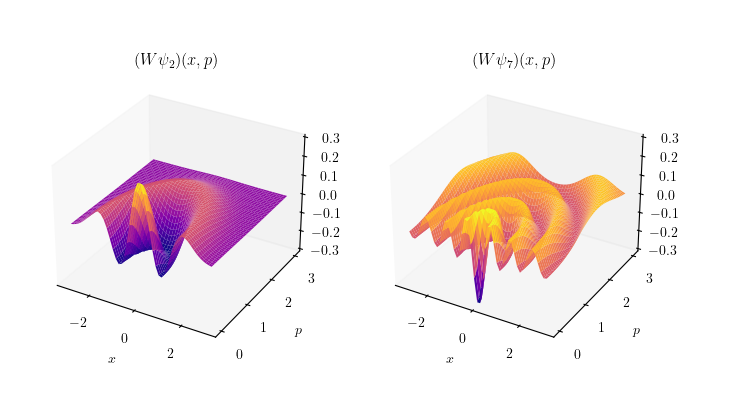
\includegraphics[width=1\textwidth]{
        imgs/harmonic_osc_wigner.png
      }
      \caption{Funciones de Wigner de los estados $\psi_3$ y
      $\psi_7$ del oscilador armónico, con $\hbar = 1$ y
      $\omega = 1$.}
      \label{fig:harmonic_osc_wigner_3_7}
    \end{figure}
  \end{example}
  
  \subsection{La correspondencia de Stratonovich-Weyl y la
  propiedad tomográfica}

  Al inicio de éste capítulo mencionamos que existen
  diversas cuasi-distribuciones en el espacio de fase, las
  cuales son usadas para formar distintas representaciones
  de la mecánica cuántica. Algunas se pueden obtener a
  partir de las distintas maneras de extender la
  correspondencia de Wigner-Weyl entre funciones sobre
  $\R^{2n}$ y operadores sobre $L^2(\R^{n})$, a grupos de
  Lie que actúan sobre un espacio homogéneo\footnote{Dentro
    de la teoría de grupos de Lie, formalmente un espacio
  homogéneo es una variedad $\mathcal M$ con una acción lisa
  y transitiva dada por un grupo de Lie $G$.}. Éstas
  distribuciones están relacionadas por algo que se conoce
  como la \textit{correspondencia de Stratonovich-Weyl}, las
  cuales son un conjunto de propiedades o criterios
  razonables que una cuasi-distribución sobre un espacio de
  fase arbitrario debería satisfacer \cite{cahen}. 

  La idea básica es la siguiente\footnote{Los detalles no
  son importantes para nuestros objetivos, por lo cual
  hemos asumido inecesario definir a los objetos que aperecen
  enseguida.}. Sea $G$ un grupo de Lie y
  $\pi$ una representación unitaria de $G$ sobre el espacio
  de Hilbert $\H$. Sea $\mathcal M$ un $G$-espacio homogéneo
  y sea $\mu$ una medida $G$-invariante sobre $\mathcal M$.
  La correspondencia de Stratonovich-Weyl es un isomorfismo
  $W$ del espacio de operadores sobre $\H$ al espacio de
  funciones sobre $\mathcal M$ que satisface las siguientes
  propiedades:
  \begin{enumerate}
    \item $W$ mapea al operador de identidad de $\H$ a la
      función constante $1$.
    \item La función $W(A^{*})$ es el conjugado complejo de
      $W(A)$.
    \item $W$ satisface la propiedad de covarianza:
      \begin{equation}
        W\left(\pi(g) A \pi(g)^{-1}\right)(u)
        = W(A)\left( g^{-1} u \right). 
      \end{equation}
    \item $W$ satisface la propiedad de la traza:
      \begin{equation}
        \int_{\mathcal M} W(A)(u) W(B)(u) \, d\mu(u)
        = \Tr(AB),
      \end{equation}
      para dos operadores $A$ y $B$.
  \end{enumerate}
  Notemos que la correspondencia de Weyl es un caso
  particular de la correspondencia de Stratonovich-Weyl.  En
  éste caso $G$ es el grupo de Heisenberg actuando sobre
  $\R^{2n}$ y $\pi$ es la representación del grupo de
  Heisenberg, i.e., los operadores de Heisenberg-Weyl. El
  isomorfismo es la transformación de Wigner
  (equivalentemente, la transformación de Weyl), la cual
  satisface los criterios como hemos visto en la sección
  anterior.

  Los criterios de Stratonovich-Weyl pueden ser expresados
  en términos de un \textit{núcleo} integral, el cual es una
  función $\Omega$ de $\mathcal M$ al espacio de operadores
  de $\H$, tal que:
  \begin{enumerate}
    \item $\Omega(u)$ es auto-adjunto.
    \item $\Omega(u)$ es de traza unitaria.
    \item El núcleo satisface una propiedad de covarianza:
      \begin{equation}
        \pi(g) \Omega(u) \pi(g)^{-1}
        = \Omega(g u),
      \end{equation}
      para todo $g \in G$.
    \item Satisface la ecuación:
      \begin{equation}
        \int_{\mathcal M} \Tr\left( \Omega(u)\Omega(v)
        \right) \Omega(v) \, d\mu(v)
        = \Omega(u).
      \end{equation}
  \end{enumerate}
  En nuestro caso, el núcleo está dado por los operadores
  puntuales $\hat\Delta(x,p)$. En el siguiente capítulo
  definiremos la función de Wigner para sistemas discretos,
  y seremos guiados por versiones análogas de las
  propiedades de Stratonovich-Weyl para la función de Wigner
  y para los operadores puntuales.

  Ahora, existen algunas propiedades de la función de Wigner
  que la distingue de otras cuasi-distribuciones. En
  particular, satisface una a la que Wootters
  \cite{wootters1987} le llama \textit{propiedad
  proyectiva}.
  \begin{proposition}
    \label{prop:proy_prop}
    Si $W_\rho$ es la función de Wigner de un estado $\rho$,
    entonces podemos considerar la integral de $W_\rho$
    sobre una franja infinita delimitada por dos rectas
    paralelas $ax+bp=c_1$ y $ax+bp=c_2$.  Resulta que la
    integral es igual a la probabilidad de que se observe un
    valor entre $c_1$ y $c_2$ del observable $a \hat X + b
    \hat P$. 
  \end{proposition}
  Ésta propiedad proyectiva se puede expresar en términos de
  los operadores puntuales. Las siguientes expresiones son
  formales e ignoramos los detalles de rigor que pudieran
  presentarse.
  \begin{proposition}
    Para todo $x,p \in \R^{n}$ los operadores puntuales
    $\hat\Delta(x,p)$ satisfacen las siguientes propiedades:
    \begin{enumerate}
      \item Son ``ortogonales'' en el siguiente sentido:
        \begin{equation}
          \Tr\left( \hat\Delta(x,p)\hat\Delta(x',p') \right) 
          = \frac{1}{2\pi} \delta(x-x')\delta(p-p').
        \end{equation}
      \item Integrando el operador puntual $\hat\Delta(x,p)$
        sobre una recta $ax+bq = l$ en el espacio de fase
        nos brinda una proyección correspondiente al
        eigenestado de $a\hat X + b \hat P$ con eigenvalor
        $l$:
        \begin{equation}
          \int_{\R^2} \hat\Delta(x,p) \delta(ax+bq-l) \, dx
          \, dp = \Pi_l.
        \end{equation}
    \end{enumerate}
  \end{proposition}
  La noción de un producto de deltas no tiene mucho sentido,
  pero la expresión análoga para el caso discreto está bien
  definida. La segunda propiedad nos dice que integrando el
  operador puntual sobre una linea en el espacio de fase,
  obtenemos una proyección. Como consecuencia, integrando la
  función de Wigner sobre una recta obtenemos una ``densidad
  marginal'' en la dirección de la linea recta. Ésto es una
  generalización de las densidades de posición y de momentum
  y se ha demostrado que imponiendo ésta propiedad a una
  cuasi-distibución adecuada del espacio de fase, se obtiene
  la distribución de Wigner, en otras palabras, ésta
  restricción adicional la vuelve única entre las
  cuasi-distribuciones \cite{ellinas2008}. Si tenemos un
  conjunto completo de éstas ``marginales generalizadas'',
  es decir, para todas las direcciones, podemos recuperar la
  distribución conjunta sobre todo el espacio en un proceso
  de tomografía cuántica.
  \begin{definition}
    \label{def:tomo_prop}
    Dado un conjunto completo de densidades marginales, es
    posible recuperar la función de Wigner. A ésta propiedad
    se le conoce como la propiedad tomográfica de la función
    de Wigner.
  \end{definition}
  El término \textit{completo} tiene un significado más
  preciso, pero no trivial, corresponde a una cantidad
  mínima de densidades marginales requeridas para la
  construcción completa del \textit{tomograma}
  \cite{ibort2009}. La representación tomográfica de estados
  cuánticos está basada en la transformación de Radon de la
  función de Wigner \cite{degosson2022}. En la tomografía
  convencional (la tomografía médica), se recolectan datos
  en forma de densidades marginales. En el plano, una
  marginal es la proyección de una función sobre el plano en
  la \textit{dirección} indicada por un ángulo.  La
  colección de marginales para distintos ángulos es la
  \textit{transformación de Radon} de dicha
  función\footnote{Resulta que las mediciones utilizadas son
    ``mutuamente conjugadas'' en el sentido de que los
    eigenestados de los operadores $a \hat X + b \hat p$ nos
    brindan una distribución uniforme del valor de $a' \hat
    x + b' \hat p$ siempre y cuando los vectores $(a,b)$ y
    $(a',b')$ sean en distintas direcciones. Notemos la
    similitud con el procedimiento de la determinación de
  estados mediante mediciones con bases mutuamente
  insesgadas.}. En el contexto de la mecánica cuántica tenemos
  la siguiente definición. 
  \begin{definition}
    La transformación de Radon $\mathcal R_{\rho}$ de una
    función de Wigner $W_\rho$ de un estado $\rho$, está
    dada por
    \begin{equation}
      \mathcal R_{\rho}\left( X, \mu, \nu \right) 
      = \int_{\R^2} W_\rho(x,p) \delta(X - \mu x - \nu p)
      \, dx \, dp.
    \end{equation}
    La transformación de Radon es invertible (bajo ciertas
    condiciones):
    \begin{equation}
      W_\rho(x,p)
      = \frac{1}{2\pi \hbar}
      \int_{\R^3} \mathcal R_{\rho}(X, \mu, \nu)
      e^{\frac{i}{\hbar}\left( X - \mu x - \nu p \right)} \,
      dX \, d\mu \, d\nu.
    \end{equation}
  \end{definition}
  Experimentalmente se mide la transformación de Radón por
  medio de un proceso llamado el \textit{método
    homodino}\footnote{La palabra \textit{homodino} se
  refiere a una comparación entre una luz que se mide contra
  una luz de referencia de la misma frecuencia.}. Al
  obtener una aproximación adecuada del tomograma, se
  invierte la transformación de Radon para obtener la
  función de Wigner.  Como ya sabemos, la función de Wigner
  es un representación completa del estado cuántico asi que
  solo queda decidir si hacer mecánica cuántica en el
  espacio de fase o recuperar el operador de densidad y
  trabajar en el espacio de Hilbert. Ésto concluye el
  proceso de la tomografía cuántica.
  
  A parte de versiones discretas de las propiedades de
  Stratonovich-Weyl, la propiedad tomográfica será
  fundamental en la construcción de una función de Wigner
  discreta bajo la metodología de Wootters. Dicha
  construcción será el contenido del siguiente capítulo.

  \chapter{Funciones de Wigner en el Espacio Fase Discreto}

  %Resumiendo el capítulo anterior, sabemos que podemos
  %representar a un estado cuántico en el espacio de fase por
  %medio de la cuasi-distribución de Wigner. A pesar de no ser
  %una densidad probabilística verdadera sobre el espacio de
  %fase, comparte varias propiedades, en particular nos
  %permite calcular los valores esperados de observables
  %cuánticos y nos permite recuperar las densidades
  %apropiadadas.

  Durante las últimas decadas han existido múltiples
  intentos de generalizar la función de Wigner a sistemas
  cuánticos de dimensión finita. Parte fundamental de ésta
  generalización es la definición adecuada del espacio de
  fase discreto. Para un sistema de dimensión $d$, la
  mayoría de construcciones emplean una malla de tamaño $d
  \times d$ e intentan definir una función de Wigner
  evaluada en cada punto $\alpha$ de la malla. Como menciona
  Gross \cite{gross2005}, parece que existen dos caminos
  claros en la construcción de la versión discreta: un
  camino intenta definir la función de Wigner discreta de
  una manera análoga a la versión continua, i.e.,
  identificando el espacio de fase discreto con las
  variables de posición y de momentum, construyendo los
  operadores de desplazamiento y luego los puntuales, para
  luego definir la función por medio del valor esperado del
  operador puntual en el estado cuántico. La ventaja de éste
  camino es que la definición discreta asemeja lo más
  posible al caso continuo y a sus a interpretaciones. Ésta
  versión se puede encontrar en los trabajos de Klimov,
  Sanches y Soto \cite{klimov2005}, Paz \cite{paz}, Vourdas
  \cite{vourdas2005}, Gross \cite{gross2005}, etc. El
  segundo camino dominante es el que intenta definir la
  función discreta a partir de la preservación de las
  propiedades más importantes del caso continuo, en
  particular la propiedad tomográfica. Ésta versión se debe
  a Wootters \cite{gibbons2004} y la idea es identificar una
  \textit{estructura cuántica} al espacio de fase discreto,
  la cual permite que la función de Wigner exprese las
  mismas propiedades que la versión continua.  Los
  operadores de desplazamiento y los puntuales vuelven a
  aparecer, pero se introduce un tipo de arbitrariedad y de
  flexbilidad, perdiendo la unicidad pero permitiendo una
  construcción alternativa. Además ésta segunda metodología
  expone una relación directa con la construcción de bases
  mutuamente insesgadas.

  Se sabe que el número máximo de bases mutuamente
  insesgados para un sistema cuántico de dimensión $d$ es
  $d+1$, y en particular si la dimensión es una potencia de
  un número primo, entonces siempre se puede alcanzar la
  cantidad máxima \cite{gibbons2004}. Parece que aun es un
  problema abierto identificar la cantidad máxima para
  dimensiones que no son potencias de números primos. La
  construcción de Wootters requiere de la construcción
  explícita de las $d+1$ MUBs para la definición de los
  operadores puntuales y como consecuencia la definición de
  la función de Wigner. Ésto es una consecuencia natural de
  exigir que la función discreta satisfaga las mismas
  propiedades tomográficas que satisface la versión
  continua. Por éstas razones nuestro trabajo se basa en la
  metodología de Wootters.
  %\section{Construcción análoga}

  %Tal como en el caso continuo, existe un mapeo del espacio
  %de Hilbert al espacio de fase que se puede interpretar
  %como una cuasi-distribución conjunta sobre dos variables
  %`conjugadas'. Schwinger desarrolló una base ortonormal de
  %$N^2$ operadores unitarios que forman una representación
  %del grupo de Heisenberg-Weyl modulo su centro. Dado la
  %base ortonormal de operadores, se puede describir al
  %estado de un sistema utilizando los coeficientes de la
  %expansión del operador de densidad en términos de la base.
  %El trabajo consiste en elegir a la ``mejor'' base que
  %resulte en las propiedades de la función de Wigner que
  %deseamos preservar.  La idea de Wooters es construir una
  %versión discreta de los operadores puntuales que preservan
  %las propiedades. 

  %Empezando con la transformada de Fourier discreta y
  %restringiendonos a dimensiones primas impares, podremos
  %trabajar en analogía al caso continuo. El grupo de
  %desplazamientos de Heisenberg-Weyl nos darán los
  %operadores de paridad desplazados, los cuales se usarán
  %para asignar puntos del espacio de fase a operadores.

  %Un sistema cuántico con una espacio de Hilbert de
  %dimensión $N$ será representado por un arreglo de $N
  %\times N$ puntos. Los puntos $\alpha$ estarán dados por
  %los pares $(a_1,a_2)$ de elementos de un campo finito
  %$\Z_n$.

  %Existe una base ortonormal de $N$ elementos para nuestro
  %espacio de Hilbert, correspondientes a los eigenestados de
  %algún observable. Denominemos a éste observable como la
  %``posición'' y diagramaticamente denotará el eje
  %horizontal. Sus eigenvalores denotarán la coordenada del
  %eje horizontal. Lo que sigue es identificar las lineas
  %perpendiculares al eje horizontal del espacio de fase con
  %los eigenestados que corresponden a los eigenvalores. El
  %eje vertical será la variable Fourier-conjugada de la
  %posición llamada el ``momentum''.

  \section{Construcción de Wootters}

  En su artículo del 2004 \cite{gibbons2004}, Wootters
  comienzan notando que la función de Wigner en sistemas
  continuos puede ser obtenida al exigir una estructura
  cuántica al espacio de fase. Ésta estructura corresponde a
  la asignación de estados cuánticos a rectas en el espacio
  de fase, de tal manera que las integrales sobre éstas
  rectas o franjas de rectas nos dan la probabilidad de
  observar el sistema en el estado correspondiente, tal como
  se mencionó en la sección anterior. Con ésta asignación,
  es posible recuperar los operadores puntuales y así
  construir la función de Wigner para un estado arbitrario
  $\rho$.  Wootters intentan definir una versión discreta
  siguiendo éstos pasos, cuidando que la construcción
  preserve otras propiedades de la versión continua.
  Resulta que su método introduce cierto tipo de
  arbitrariedad por lo que acaban definiendo distintas clase
  de funciones discretas.

  Evidentemente hay una relación directa entre la geometría
  del espacio de fase y la estructura cuántica por asignar.
  Por lo tanto requerimos trabajar con un espacio de fase
  que tenga la suficiente estructura geométrica como para
  definir rectas en el espacio con las propiedades usuales
  que conocemos del plano Euclideano.  Por ejemplo debemos
  poder definir rectas paralelas y se debe cumplir que dos
  rectas no paralelas solo se intersecten en un solo punto.
  Si $d$ es la dimensión del espacio de Hilbert en cuestión,
  es natural intentar definir el espacio de fase como la
  malla $\Z_d \times \Z_d$. Pero si $d$ no es un número
  primo, $\Z_d$ solo es un anillo y resulta que el espacio
  $\Z_d \times \Z_d$ no tiene la estructura geométrica
  necesaria, por ejemplo no es dificil encontrar ejemplos de
  rectas no paralelas que se intersectan en más de un solo
  punto. En el caso en que $d = p$ es un número primo, la
  estructura algebráica $\Z_p$ es un campo y aquí sí se
  puede definir un espacio de fase $\Z_p \times \Z_p$ con
  las propiedades deseadas.  Además de los campos $\Z_p$,
  también podemos obtener campos de orden $p^{n}$ donde $p$
  es primo, por medio de la extension de Galois
  $\GF\left(p^{n}\right)$.  La restricción a espacios de
  Hilbert dimensión $p^{n}$ sí es limitante, pero Wootters
  hace la observación que su método es válido para el
  importante caso de un sistema de $n$ qubits. Por lo tanto
  su metodología es directamente aplicable a los modelos de
  la computación e información cuántica.

  El método consiste en darle una estructura cuántica al
  espacio de fase discreto $\F \oplus \F$ asignando un
  estado cuántico a cada linea del espacio.  Ésta asignación
  debe satisfacer varias propiedades y aquellas que las
  satisfacen se llaman, \textit{`mallas cuánticas'}. Cada
  malla cuántica define una versión de la función de Wigner,
  pero es posible hacer una clasificación en clases de
  equivalencia para reducir un poco la arbitrariedad. La
  asignación particular de estados cuánticos a las rectas de
  conjuntos de rectas paralelas resultan ser bases
  ortonormales del espacio de Hilbert y además son
  mutuamente insesgadas respecto a otros conjuntos de rectas
  paralelas.

  Para comenzar, recordemos las propiedades de la función de
  Wigner del caso continuo que se deseamos perservar en el
  caso discreto, las primeras tres son las propiedades de
  Stratonovich-Weyl y la cuarta es la propiedad tomográfica
  de la función de Wigner:
  \begin{proposition}
    Sea $\rho$ un operador de densidad y $W_\rho$ su función
    de Wigner.
    \begin{enumerate}
      \item $W_\rho$ es covariante bajo traslaciones.
      \item Los operadores puntuales forman una base
        ortonormal respecto al producto interno de
        Hilbert-Schmidt para el espacio de operadores sobre
        $\H$.
      \item $W_\rho$ es real y la integral sobre todo el
        espacio de fase es igual a $1$.
      \item La integral de $W_\rho$ sobre una
        recta $ax+bp = c$ nos brinda la probabilidad de
        medir el valor $c$ del operador $a \hat X + b \hat P$.
    \end{enumerate}
  \end{proposition}
  Recordemos que éstas propiedades pueden ser demostradas a
  partir de las propiedades análogas de los operadores
  puntuales. En el caso continuo la propiedad proyectiva
  está relacionada directamente con los operadores $a \hat X
  + b \hat P$, en el caso discreto ésto ya no es el caso. De
  hecho, la asignación de un significado físico a los ejes
  del plano discreto es algo arbitrario. Como veremos más
  adelante, elegimos una base ortonormal arbitraria la cual
  se asigna al ``eje horizontal''. La base asignada al ``eje
  vertical'' será mutuamente insesgada a la horizontal,
  preservando de algun modo ésta idea de complementariedad.
  Eligiendo las bases correctamente para el resto de las
  rectas del espacio nos permitirá reconstruir un estado
  cuántico por medio de probabilidades medidas, tal como
  sucede en la tomografía cuántica en el caso continuo. Por
  otro lado, la propiedad de ser covariante bajo
  traslaciones surge naturalmente a partir de las
  propiedades de los operadores de desplazamiento y éstos
  son clave en la construcción de las bases.
    
  \subsection{La geometría del espacio de fase discreto}

  El espacio de fase discreto será un espacio vectorial de
  dos dimensiones sobre un campo finito $\F$, donde los
  puntos serán etiquetados con los elementos $(x,p) \in \F
  \oplus \F$. Por convención, consideramos el punto $(0,0)$
  como el origen de nuestra malla de $d \times d$ elementos,
  ubicado en la parte inferior izquierda. La construcción de
  Wootters y Gibbons permite identificar el eje horizontal
  con los eigenvectores de una clase de operadores y el eje
  vertical con otra clase de operadores, ésto a su vez nos
  permite darle cierta interpretación física, aunque la
  asignación no es naturalmente única. Por ejemplo si
  consideramos un sistema cuántico de dos partículas con
  spin-$\frac{1}{2}$, entonces el espacio de Hilbert
  correspondiente es $\H = \C^{2} \otimes \C^{2}$, y el
  espacio de fase discreto sería una malla de $4 \times 4$
  elementos. Salvo isomorfismos, el campo finito de cuatro
  elementos es único y lo identificamos con la extensión de
  Galois $\GF\left(2^2\right)$. Los elementos de la malla
  serán indexados por los elementos de éste campo:
  \[
    \F
    = \GF\left(2^2\right)
    = \{0,1,\alpha,\alpha+1\}.
  \]
  En caso de un sistema que no es compuesto, por ejemplo una
  partícula de tres niveles, $\H = \C^3$, el espacio de fase
  discreto es una malla de $3 \times 3$ en donde los
  elementos de la malla son indexados simplemente con los
  enteros módulo 3, $\F = \Z_3 = \{0,1,2\}$. La figura
  (\ref{fig:GF22-GF31}) muestra el espacio de fase de éstos
  dos ejemplos, y se muestra la linea recta parametrizada
  como 
  \[
    \lambda = \{(s,s) : s \in \F\},
  \]
  la cual corresponde con la noción de un rayo diagonal en
  el plano Euclideano.
  \begin{figure}
    \centering
    \subfloat[\centering $\F \times \F$ donde $\F =
    \GF(2,2)$.]{{
        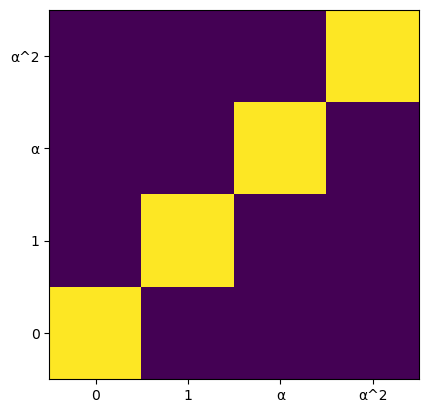
\includegraphics[width=0.38\linewidth]{imgs/GF22.png}
    }}
    \quad
    \subfloat[\centering $\F \times \F$ donde $\F =
    \Z_3$.]{{
        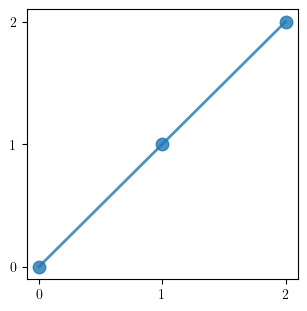
\includegraphics[width=0.35\linewidth]{imgs/GF31.png}
    }}
    \caption{Dos espacios de fase discretos para sistemas de
    distinta dimensión, señalando el rayo diagonal $y = x$.}
    \label{fig:GF22-GF31}
  \end{figure}
  De manera general, una \textit{recta} en el espacio
  de fase es el conjunto de puntos que satisfacen la
  ecuación $ax + bp = c$ donde $a,b$ y $c$ son elementos del
  campo finito. Dos rectas paralelas son iguales si solo
  difieren en el valor de $c$.  No es dificil probar que
  dada una recta $\lambda$ y un punto $\alpha$ que no
  pertenece a la recta existe una única recta paralela a
  $\lambda$ que contiene a $\alpha$.  Similarmente, dos
  rectas que no son paralelas solo se intersectan en un solo
  punto. Existen $d(d+1)$ rectas en el espacio de fase y el
  conjunto de éstas rectas se particiona en $d+1$ conjuntos
  de $d$ rectas paralelas. A cada conjunto de $d$ rectas
  paralelas, se le conoce como un \textit{estría}. 

  Para ejemplifcar un conjunto completo de estrías de un
  espacio de fase discreto, consideremos un campo finito de
  ocho elementos. En éste caso el espacio de fase es el
  espacio vectorial $\F \oplus \F$ donde $\F =
  \GF\left(2^3\right)$ es una extensión de Galois del campo
  primo $\Z_2$ de grado $n = 3$. De acuerdo al apéndice
  (\ref{sec:fields}), para construir a $\F$ solo debemos
  elegir un polinomio irreducible $f(x)$ con coeficientes en
  $\Z_2$ de grado $n = 3$ y adjuntarle una raíz $\alpha$ del
  polinomio al campo primo. Equivalentemente podemos tomar
  el cociente del anillo de polinomios $\Z_2[x]$ con el
  ideal generado por el polinomio irreducible:
  \begin{equation}
    \F
    = \mathbb Z_2(\alpha)
    \cong \mathbb Z_2[x] / \langle f(x) \rangle.
  \end{equation} 
  Sea $f(x) = x^3+x^2+1$ tal polinomio irreducible y
  $\alpha$ una raíz primitiva\footnote{Todos los polinomios
  elegidos en éste trabajo son los de Conway}. Entonces el
  campo finito $\F$ está dado por el conjunto
  \begin{equation}
    \F
    = \{
      0, 1, \alpha, \alpha^2, \alpha+1, \alpha^2+\alpha,
      \alpha^2 + \alpha + 1, \alpha^2 + 1
    \},
  \end{equation} 
  con sus correspondientes operaciones de suma y
  mutliplicación. Las rectas verticales estarán dadas por
  los conjuntos $\{(x,y) : y \in \F\}$ donde fijamos el
  elemento $x$ para cada recta vertical. El resto de las
  rectas pueden ser parametrizadas como $\{(x,mx+c) : m, c
  \in \F\}$. La figura (\ref{fig:GF-2-3}) muestra todas las
  estrías de éste espacio de fase.
  \begin{figure}[ht]
    \centering
    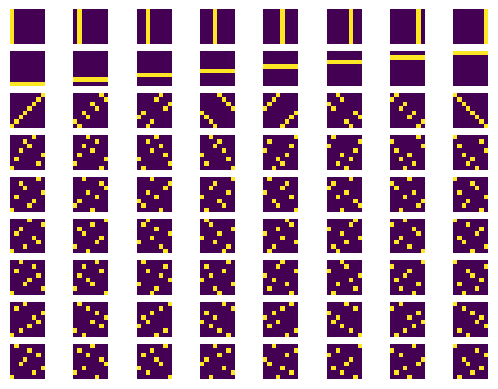
\includegraphics[width=0.7\textwidth]{imgs/GF23.png}
    \caption{Las nueve estrías del espacio de fase sobre el
    campo $\F = \GF\left(2^3\right)$. La primera columna
    consta de los rayos y el resto de las columnas
    representan las traslaciones paralelas de cada rayo.}
    \label{fig:GF-2-3}
  \end{figure}
  Otro aspecto importante inicial en la metodología de
  Wootters es la noción de las traslaciones en el espacio de
  fase. En el caso discreto no existen traslaciones
  infinitesimales, pero podemos definir una traslación como
  la suma de un vector a los puntos del espacio de fase. Si
  $(a,b) \in \F \oplus \F$, entonces la traslación $\mathcal
  T(a,b)$ se define simplemente como
  \begin{equation}
    \mathcal [T(a,b)](c,d) = (a+c, b+d),
    \quad
    \text{para todo } (c,d) \in \mathbb F \oplus \F.
  \end{equation} 
  Se sigue inmediatamente que la composición de traslaciones
  en el espacio de fase discreto se rige bajo la siguiente
  regla. Para todo $(a,b), (c,d) \in \F \oplus \F$ tenemos
  que
  \begin{equation}
    \label{eqn:translation_composition}
    \mathcal T(a,b) \circ \mathcal T(c,d)
    = \mathcal T(a+c,b+d).
  \end{equation}
  La metodología de Wootters inicia haciendo una
  correspondencia entre las traslaciones en el espacio de
  fase con operadores en el espacio de Hilbert, de manera
  análoga al caso continuo. En el artículo original, no
  mencionan las representaciones unitarias del grupo de
  traslaciones a la hora de definir a los operadores de
  desplazamiento, ya que para asignar la malla cuántica no
  es necesario utilizar a toda la representación pues las
  fases globales se ignoran. Para ver una construcción más
  fiel al caso continuo recomendamos ver el trabajo de
  Vourdas \cite{vourdas2005}.

  \subsection{Asignación de la estructura cuántica}

  Para vincular el sistema cuántico con nuestro espacio de
  fase discreto, la clave del método Wootters y Gibbons es
  asignar un estado cuántico a cada una de las $d(d+1)$
  lineas rectas del espacio de fase. De aquí en adelante
  consideramos un sistema cuántico modelado por un espacio
  de Hilbert de dimensión $d = p^{n}$ donde $p$ es un número
  primo. Éste método es aplicable de manera natural a
  sistemas compuestos de $n$ subsistemas de dimensión $p$:
  \begin{equation}
    \H^{\otimes n}
    = \H \otimes \cdots \otimes \H,
    \quad
    \text{donde } \dim\H = p.
  \end{equation}
  Sea $Q$ la malla cuántica, la cual asigna una proyección
  ortogonal correspondiente a un estado puro $Q(\lambda)$, a
  cada recta $\lambda$ y que satisface ciertas propiedades.
  La primera propiedad que debe satisfacer la malla cuántica
  es la propiedad de ser covariante bajo traslaciones, para
  ésto, debemos definir una versión discreta de los
  operadores de Heisenberg-Weyl $\hat D(x,p)$ para cada
  $(x,p) \in \F \oplus \F$. De ésta manera a cada traslación
  en el espacio de fase discreto le corresponderá un
  operador unitario en el espacio de Hilbert. Éstos
  operadores deben tener una regla de composición que
  preserve de algún modo la composición de traslaciones en
  el espacio de fase. 

  Como mencionamos en la sección anterior, Wootters et al no
  mencionan a los operadores de Heisenberg-Weyl como
  comunmente se hace en el caso continuo. En su lugar,
  construyen a los operadores de desplazamiento de una
  manera ad-hoc, enfocándose en sistemas de dimensión prima,
  en donde el espacio de fase discreto es simplemente el
  campo finito $\F = \Z_p$, y luego utilizando el producto
  tensorial para obtener los operadores para dimensiones
  compuestas. Comenzamos por definir a dos operadores
  básicos, correspondientes a traslaciones horizontales y
  verticales de una unidad. A la traslación horizontal del
  espacio de fase $\mathcal T(1,0)$ y la traslación vertical
  $\mathcal T(0,1)$ les asociamos los operadores unitarios
  $X$ y $Z$ definidos de la siguiente manera:
  \begin{definition}
    Sea $\{\ket k : k \in \Z_p\}$ una base ortonormal del
    espacio de Hilbert $\mathcal H$ correspondiente a un
    subsistema (generalmente usaremos la base estándar).
    Etiquetamos a los vectores con los elementos del campo
    primo. Entonces definimos los operadores $X$ y $Z$ como
    \begin{align}
      X \ket k
      &= \ket{k + 1}, \\
      Z \ket k
      &= \omega^{k} \ket k,
    \end{align}
    donde $\omega = e^{2\pi i / p}$ y donde la suma dentro
    de los kets se hace módulo $p$, i.e., la suma es la del
    campo finito $\Z_p$.
  \end{definition}
  El uso de los números del campo primo como etiquetas
  implica una estructura cíclica a las potencias del
  operador $X$ y comunmente se le llama el operador
  \textit{shift} porque en el caso continuo representan
  cambios en la posición. Similarmente el operador $Z$ se le
  conoce como el operador \textit{boost} porque en el caso
  continuo representa un empuje en términos del momentum.
  Podemos expresar a éstos operadores en la base
  estándar de la siguiente manera:
  \begin{equation}
    X = \sum_{k \in \Z_p}^{} \ket{k+1}\bra{k}, \\
    \quad
    Z = \sum_{k \in \Z_p}^{} \omega^{k} \ket k \bra k.
  \end{equation}
  Es fácil probar las siguientes propiedades de los
  operadores $X$ y $Z$:
  \begin{proposition}
    \label{prop:prime_XZ_props}
    Sea $\ket k$ un elemento de la base estándar y $a,b \in
    \F$, entonces
    \begin{enumerate}
      \item $X^{a} \ket{k} = \ket{k+a}$ y $Z^{b} \ket{k} =
        \omega^{b k} \ket{k}$.
      \item $X^{p} = Z^{p} = 1$, $X^{a} Z^{b} = \omega^{-ab}
        Z^{b} X^{a}$, y $\Tr(X) = \Tr(Z) = 0$.
    \end{enumerate}
  \end{proposition}
   
  \begin{example}
    En el caso de dimensión $p = 2$, los monomios de $X$ y
    $Z$ son elementos del \textit{grupo de Pauli}. En
    particular las matrices $X$ y $Z$ son simplemente las
    matrices de Pauli $\sigma_x$ y $\sigma_z$:
    \[
      X = \sigma_x =
      \begin{pmatrix} 0 & 1 \\ 1 & 0 \end{pmatrix},
      \quad
      Z = \sigma_z =
      \begin{pmatrix} 1 & 0 \\ 0 & -1 \end{pmatrix}. 
    \] 
  \end{example}
  La matriz $Z$ es diagonal en la base estándar por lo tanto
  sus eigenvectores son simplemente los elementos $\ket k$.
  La matriz $X$ es diagonal respecto a la siguiente base:
  \[
    \ket{\tilde j}
    = \frac{1}{\sqrt{p}} \sum_{k \in \Z_p}^{}
    \omega^{j k} \ket k,
  \] 
  donde la tilde se usa para distingir ésta base de la base
  estándar. Notemos que ésta última expresión parece una
  transformación de Fourier de la base computacional. De
  hecho Vourdas y otros autores definen una transformación
  de Fourier finita a partir de los caracteres aditivos
  $\chi$ del campo finito y construyen una segunda base del
  espacio de Hilbert mediante su aplicación. De ésta manera
  obtienen dos bases `Fourier conjugables' y las asocian con
  la noción de posición (base computacional) y momentum
  (base obtenida por la transformación de Fourier) en el
  espacio de fase discreto. A pesar de ésto Klimov et al.
  hacen la observación que debido a la arbitrariedad de las
  bases, la analogía con la posición y momentum en el
  espacio de fase discreto es un poco forzada
  \cite{bjork2008}. Otra propiedad interesante de éstas dos
  bases surge del siguiente cálculo:
  \begin{equation}
    \braket{m|\tilde j}
    = \frac{1}{\sqrt{p}}
    \sum_{k \in \Z_p}^{} \omega^{jk} \braket{m|k}
    = \frac{1}{\sqrt{p}} \omega^{jm},
  \end{equation}
  por lo tanto $\left|\braket{m|\tilde j}\right|^2 =
  \frac{1}{p}$. En otras palabras, las bases $\ket k$ y
  $\ket{\tilde j}$ son mutuamente insesgadas. Más adelante
  construiremos más bases a partir de subconjuntos de los
  operadores de desplazamiento y para sistemas con dimensión
  $p^{n}$, todas éstas bases serán mutuamente insesgadas.

  Los operadores de desplazamiento están en correspondencia
  con las traslaciones del espacio de fase discreto. Sean
  $a,b \in \F$, utilizando la proposición
  (\ref{prop:prime_XZ_props}) naturlamente definimos a los
  operadores de desplazamiento correspondientes a una
  traslación $\mathcal T(a,b)$ como 
  \begin{equation}
    D(a,b)
    = X^{a} Z^{b},
  \end{equation}
  cuya acción sobre los elementos de la base estándar es
  \[
    D(a,b) \ket{k}
    = X^{a} Z^{b} \ket k
    = X^{a} \omega^{bk} \ket k
    = \omega^{bk} \ket{k+a}.
  \] 
  Recordemos que para todo $(a,b), (c,d) \in \F \oplus \F$,
  las traslaciones satisfacen la regla de composición en
  (\ref{eqn:translation_composition}), similarmente, los
  operadores de desplazamiento satisfacen la siguiente
  propiedad de composición:
  \begin{align}
    D(a,b) D(c,d)
    &= \left( X^{a}Z^{b} \right) \left( X^{c}Z^{d} \right)
    \\
    &= \omega^{c b} X^{a} X^{c} Z^{b} Z^{d} \\
    &= \omega^{c b} X^{a+c} Z^{b+d} \\
    &= \omega^{c b} D(a+c, b+d).
  \end{align}
  Por lo tanto, salvo una fase global, la composición de los
  operadores $D(a,b)$ es análoga a la de las traslaciones en
  el espacio de fase.

  Hasta ahorita solo hemos trabajado con sistemas de
  dimensión prima. En el siguiente capítulo se definirán los
  operadores $X$ y $Z$ para sistemas de dimensión $p^{n}$,
  en donde la base ortonormal elegida es etiquetada con
  elementos de la extensión de Galois. Mediante el uso de
  bases del campo finito, se pueden factorizar los
  operadores de desplazamiento y de sus eigenvectores.
  Wootters y Gibbons deciden trabajar de una manera inversa,
  ellos definen los operadores de desplazamiento para
  sistemas de dimensión $p^{n}$ \textit{directamente} del
  producto tensorial de monomios de $X$ y $Z$ para los
  subsistemas de dimensión $p$. Ésto involucra la elección
  de una base en el campo finito, lo cual introduce cierta
  arbitrariedad. La asociación del punto $(a,b) \in \F
  \oplus \F$ con el operador correspondiente del espacio
  $\H^{\otimes n}$ depende de la expansión de $a$ y de $b$
  en bases de la extensión de Galois.  Recordemos que la
  extensión de Galois $\GF\left(p^{n}\right)$ se puede ver
  como un espacio vectorial de dimensión $n$ sobre el campo
  primo $\Z_p$.  Eligiendo una base de la extensión
  $\{b_1,\ldots,b_n\} \subset \GF\left(p^{n}\right)$,
  podemos expresar a todo elemento $a \in \F$ como la
  combinación lineal:
  \[
    a = \sum_{i=1}^{n} c_i b_i,
    \quad
    \text{donde } c_i \in \Z_p.
  \] 
  De igual manera, debemos elegir una base dual a la base
  del campo finito. Recordemos del apéndice
  (\ref{sec:fields}) que una base dual es tal que
  \[
    \tr(b_i \tilde b_j) = \delta_{ij},
  \] 
  y que en muchas ocasiones podemos encontrar una base
  \textit{auto-dual}, algo que es conveniente a la hora de
  hacer los cálculos. Dada la base y la base dual, Wootters
  y Gibbons definen a los operadores de desplazamiento
  correspondientes a traslaciones arbitrarias $\mathcal
  T(a,b)$, como productos tensoriales de monomios de los
  operadores unitarios $X$ y $Z$, donde las potencias están
  dadas por los coeficientes de la expansión de $a$ en la
  base y de $b$ en la base dual:
  \begin{definition}
    Sean $a_1,\ldots,a_n$ los coeficientes de $a$ en la base
    del campo y $b_1,\ldots,b_n$ los coeficientes de $b$ en
    la base dual. Entonces definimos al operador de
    desplazamiento como
    \begin{equation}
      \label{eqn:wootters_hw_ops}
      D(a,b)
      = X^{a_1} Z^{b_1} \otimes \cdots \otimes X^{a_n}
      Z^{b_n}.
    \end{equation}
  \end{definition}
  A pesar de la aribtrariedad que ésto introduce, podemos
  ver que hay una correspondencia natural con las
  traslaciones \textit{básicas} del espacio de fase
  discreto, en el sentido de que si una traslación por el
  vector $(a,b)$ solo tiene los $i$-ésimos componentes de
  $a$ y $b$ no nulos, entonces el operador de desplazamiento
  solo actúa sobre el $i$-ésimo subsistema. Los operadores
  satisfacen varias propiedades interesantes, por ejemplo,
  forman una base del espacio de operadores lineales de
  $\H$.
  \begin{definition}
    Para un espacio de Hilbert de dimensión finita, un
    operador de Hilbert-Schmidt es un operador tal que
    $\Tr(A A^{*})$ es finito. El producto interno de
    Hilbert-Schmidt se define como 
    \begin{equation}
      \langle A, B \rangle_{HS}
      = \Tr\left( A B^{*} \right).
    \end{equation} 
  \end{definition}
  Dado que los operadores de desplazamiento son unitarios,
  son de Hilbert-Schmidt, pues la traza de la identidad es
  $d$. El hecho de que forman una base para los operadores
  lineales es consecuencia de ser ortogonales bajo el
  producto de Hilbert-Schmidt.
  \begin{proposition}
    Los operadores de desplazamiento son mutuamente
    ortogonales respecto al producto de Hilbert-Schmidt en
    el siguiente sentido:
    \begin{align}
      \Tr\left( D(a,b) D(c,d)^{*} \right) 
      &= d \delta^a_c \delta^b_d.
    \end{align}
  \end{proposition}
  \begin{proof}
    Para ver ésto primero consideremos el caso de dimensión
    prima: 
    \begin{equation}
      \Tr\left( D(a,b) \right) 
      = \sum_{k \in \Z_p}^{} \braket{k|D(a,b)|k} 
      = \sum_{k \in \Z_p}^{} \braket{k|\omega^{bk}|k+a} 
      = \sum_{k \in \Z_p}^{} \omega^{bk} \braket{k|k+a}.
    \end{equation}
    Si $a \neq 0$ entonces $\braket{k|k+a} = 0$ para todo $k
    \in \Z_p$. Si $a = 0$ entonces 
    \[
      \Tr\left( D(a,b) \right) 
      = \sum_{k \in \Z_p}^{} \omega^{bk},
    \] 
    por lo tanto al menos que $a = b = 0$, la traza se
    anula.  Así que
    \begin{equation}
      \label{eqn:trace_of_D}
      \Tr\left( D(a,b) \right) 
      = d \delta^a_0 \delta^b_0.
    \end{equation} 
    Por otro lado no es dificil probar que $D(a,b)^{*} =
    \omega^{ab} D(-a,-b)$, así que 
    \begin{align}
      \Tr\left( D(a,b)D(c,d)^{*} \right) 
      &= \Tr\left( \omega^{cd} D(a,b) D(-c,-d) \right) \\
      &= \Tr\left( \omega^{cd} \omega^{-c b} D(a-c, b-d)
      \right) \\
      &= \omega^{cd-c b} \Tr(D(a-c,b-d)).
    \end{align} 
    De la ecuación (\ref{eqn:trace_of_D}) tenemos que que la
    traza se anula si $(a,b) \neq (c,d)$, en caso contrario
    $\omega^{cd-c b} = 1$ y obtenemos el resultado buscado.
    El caso general se sigue de las propiedades de la traza
    respecto el producto tensorial.
  \end{proof}

  Anteriormente mencionamos que el operador $Z$ es diagonal
  y sus eigenvectores son la base estándar de $\C^{p}$.
  Notemos que en el caso de dimensión $p^{n}$, los
  operadores, 
  \[
    D(0,b) = Z^{b_1} \otimes \cdots \otimes Z^{b_n},
  \] 
  también son diagonales por lo que sus eigenvectores serán
  la base estándar de $\C^{p^{n}}$, la cual a su vez se
  puede factorizar en productos tensoriales de la base
  estándar de $\C^{p}$:
  \[
    \ket{k_1} \otimes \cdots \otimes \ket{k_n},
    \quad k_1,\ldots,k_n \in \Z_p.
  \] 
  Por otro lado, se puede probar que los operadores de
  desplazamiento respecto a las traslaciones horizontales
  son
  \[
    D(a,0) = X^{a_1} \otimes \cdots \otimes X^{a_n},
  \] 
  y sus eigenvectores están dados por productos tensoriales
  de vectores $\ket{\tilde j}$.

  El concepto de factorización tensorial es muy importante
  en áreas como la óptica cuántica y en la computación
  cuántica. A pesar de ésto, la factorización de los
  operadores desplazamiento y de sus eigenvectores no es una
  parte fundamental en la construcción de la función de
  Wigner. En realidad podemos definir una base ortonormal y
  etiquetarla con elementos de la extensión de Galois
  $\GF\left(p^{n}\right)$ y luego definir los operadores de
  desplazamiento mediante su acción sobre ésta base. Ésto lo
  hacemos en el siguiente capítulo para evitar de cierto
  modo la arbitrariedad que conlleva la introducción de
  bases del campo finito. Si es necesario factorizar,
  podemos utilizar una base del campo para mapear elementos
  entre $\C^{p^{n}}$ y $\left(\C^{p}\right)^{\otimes n}$ de
  la siguiente manera
  \[
    \ket \alpha
    \mapsto \ket{\alpha_1} \otimes \cdots \otimes
    \ket{\alpha_n},
  \] 
  donde los $\alpha_1,\ldots,\alpha_n$ son los coeficientes
  de la expansión de $\alpha$ respecto a la base elegida.
  Debido a la libertad que tenemos en la elección de la base
  del campo, la factorización no es única. Klimov et al
  \cite{bjork2008} muestran que los estados etiquetados con
  los elementos de la extensión de Galois pueden ser
  mapeados a estados fisicos con propiedades de
  factorización distintas, y ésto a su vez tiene
  consecuencias físicas.
  \begin{example}
    Éste ejemplo fue tomado de \cite{bjork2008} y nos
    muestra como la factorización tensorial puede depender
    de las bases del campo finito elegidas. Consideremos un
    sistema de dos qubits, en el estado 
    \begin{equation}
      \ket \psi = \frac{\ket 0 + \ket{1}}{\sqrt{2}}.
    \end{equation}
    Utilizando la base $(1,\alpha)$ obtenemos 
    \begin{equation}
      \ket \psi \mapsto
      \frac{\ket 0 \otimes \ket 0 + \ket 1 \otimes \ket
      0}{\sqrt{2}}
      = \frac{\left( \ket 0 + \ket 1 \right) \otimes \ket
      0}{\sqrt{2}},
    \end{equation}
    mientras que la base $(\alpha,\alpha^2)$ nos brinda 
    \begin{equation}
      \ket \psi \mapsto
      \frac{\ket 0 \otimes \ket 0 + \ket 1 \otimes \ket
      1}{\sqrt{2}}.
    \end{equation}
    Como podemos observar, el primer estado tensorial es
    factorizable mientras que el segundo no lo es.
  \end{example}

  \subsection{Definición de la red cuántica}

  Regresando a la construcción de la función de Wigner,
  vamos a utilizar a los operadores de desplazamiento para
  definir el requisito de ser covariante bajo traslaciones
  que le exigimos a la función de Wigner. Recordemos que la
  función de Wigner dependerá de la malla cuántica $Q$, la
  cual es una asignación entre las lineas del espacio de
  fase discreto y estados cuánticos de $\H$: 
  \begin{equation}
    Q : \mathcal P(\F \oplus \F) \to \mathcal L(\H).
  \end{equation} 
  Por lo tanto conviene definir una propiedad análoga para
  la asignación $Q$. Naturalmente ésto lo logramos al exigir
  la preservación la estructura cuántica asignada al espacio
  de fase cuando las lineas son trasladadas, i.e., si
  trasladamos una linea $\lambda$ por $\mathcal T(a,b)$
  entonces el estado cuántico también debe ser `trasladado'
  pero por los operadores de desplazamiento
  correspondientes. Formalmente ésto implica que
  \begin{equation}
    \label{eqn:trans_cov_net}
    Q(\mathcal T(a,b) \lambda)
    = D(a,b) Q(\lambda) D(a,b)^{*}.
  \end{equation}
  Ésto resulta ser un requisito muy fuerte, ya que implica
  que los operadores correspondientes a las traslaciones que
  dejan invariantes a las rectas de una estría deben
  conmutar. Para ver ésto, supongamos que $\lambda$ es un
  rayo parametrizado por $(sx,sy)$ donde $s \in \F$.
  Entonces ésta recta y todas las rectas paralelas a ella
  son invariantes bajo las traslaciones $\mathcal T(tx,ty)$
  donde $t \in \F$:
  \begin{align*}
    \mathcal T(tx,ty) \lambda
    &= \{(tx,ty) + (sx,sy) : (sx,sy) \in \lambda \} \\
    &= \{((t+s)x, (t+s)y) : t+s \in \F \}\\
    &= \lambda.
  \end{align*} 
  Por lo tanto la condición
  (\ref{eqn:trans_cov_net}) implica que
  \[
    D(tx,ty) Q(\lambda) D(tx,ty)^{*}
    = Q(\mathcal T(tx,ty)\lambda)
    = Q(\lambda),
  \] 
  pero como los operadores $D(a,b)$ son unitarios, ésto a su
  vez significa que
  \[
    D(tx,ty) Q(\lambda) = Q(\lambda) D(tx,ty),
  \] 
  i.e., todos los operadores $D(tx,ty)$ con $t \in \F$
  conmutan con $Q(\lambda)$. Pero ésto solo sucede si los
  operadores de desplazamiento $D(tx,ty)$ para $(x,y)$ fijo
  conmutan entre si. En otras palabras, para que la red
  cuántica sea covariante bajo traslaciones, los operadores
  de desplazamiento correspondientes a las traslaciones que
  dejan las rectas de una estría invariante deben conmutar.
  Gibbons y Wootters prueban que su definición de $D(a,b)$
  satisface éste requisito si y solo si la base en que se
  expande el vector $b$ es un \textit{múltiplo} de la base
  dual. Visto desde otro punto de vista, si identificamos el
  estado cuántico con un vector del espacio de Hilbert, la
  condición (\ref{eqn:trans_cov_net}) implica que
  $Q(\lambda)$ es un eigenvector de todos los operadores
  $D(tx,ty)$. Los operadores que son diagonalizables y
  conmutan entre sí comparten un conjunto completo de
  eigenvectores. Entonces, dado que los operadores de
  desplazamiento son diagonalizables, los operadores que
  corresponden a traslaciones que dejan invariante a una
  estría en el espacio de fase discreto, son diagonalizables
  de manera simultánea. Wootters menciona que ésta base es
  única, por lo que tiene sentido asignar a cada estría su
  correspondiente base de eigenvectores.

  Recordando que los operadores son ortogonales respecto al
  producto interior de Hilbert Schmidt, el hecho de agrupar
  a los operadores de desplazamiento en subconjuntos
  conmutativos nos brinda una de las características más
  atractivas de la construcción de Wootters de la función de
  Wigner, que depende del siguiente resultado de Bandyophyay
  et al \cite{bandyopadhyay2001}:
  \begin{theorem}[Bandyophyay et al, teorema 3.2]
    \label{thm:bandy}
    Si existe una partición de $n^2-1$ matrices unitarias
    mutuamente ortogonales en $d+1$ conjuntos de $d-1$
    matrices conmutativas, entonces existen un conjunto de
    $d+1$ bases mutuamente insesgadas.
  \end{theorem}
  Notemos que la agrupación de los operadores invariantes de
  cada estría satisface ésta condición, ya que a cada estría
  le corresponde $d-1$ operadores de desplazamiento (no
  triviales) y tenemos $d+1$ estrías del espacio de fase
  discreto en total. Por lo tanto Wootters y Gibbons
  concluyen que los conjuntos de eigenvectores simultáneaos
  forman un conjunto de bases mutuamente insesgadas. No
  detallamos más sobre ésto por el momento porque se
  estudiará más fondo en el siguiente capítulo.

  Hasta ahorita solo se ha asignado una base ortonormal a
  cada estría. Para definir por completo al mapeo $Q$
  debemos identificar a cada linea de cada estría con una
  proyección ortogonal de un elemento de la base. Resulta
  que podemos asignar un elemento de la base al rayo
  $\lambda$ de la estría de manera \textit{arbitraria}. El
  resto de la asignación se determina por los mismos
  operadores de desplazamiento debido a la propiedad de ser
  covariante bajo traslaciones:
  \[
    Q(\mathcal T(x,y) \lambda)
    = D(x,y) Q(\lambda) D(x,y)^{*},
  \] 
  ya que se pueden obtener el resto de las rectas de la
  estría mediante traslaciones en el espacio de fase. Ésto
  refleja el hecho de que las traslaciones en el espacio
  de fase discreto no cambian la pendiente de las rectas,
  por lo tanto al trasladar un recta solo obtendremos otra
  recta \textit{paralela} a ella, es decir a otro elemento
  de la estría. Que la red cuántica sea covariante bajo
  traslaciones significa que los eigenestados asignados a
  una estría quedan invariantes bajo los operadores de
  desplazamiento. 
  \begin{example}
    Consideremos un qutrit. El espacio de Hilbert es
    $\C^{3}$ y el espacio de fase discreto es simplemente
    $\Z_3 \oplus \Z_3$. Como hemos visto anteriormente, el
    rayo vertical $\lambda = \{(0,u) : u \in \Z_3\}$ es
    invariante bajo las traslaciones $\mathcal T(0,u)$ para
    todo $u \in \Z_3$. El operador correspondiente es la
    matriz generalizada de Pauli dada por
    \[
      D(0,u) = Z^{u},
    \] 
    cuyos eigenvectores simplemente consiste de la base
    estándar
    \[
      \ket 0 = \begin{pmatrix} 1\\0\\0 \end{pmatrix},
      \quad
      \ket 1 = \begin{pmatrix} 0\\1\\0 \end{pmatrix},
      \quad \text{y} \quad
      \ket 2 = \begin{pmatrix} 0\\0\\1 \end{pmatrix}.
    \] 
    Para definir la red cuántica, primero asignamos el
    eigenestado $\ket 0 \bra 0$ al rayo vertical. Si
    trasladamos a $\lambda$ por \textit{cualquier} vector
    $(x,y)$ en el espacio de fase discreto, solo obtendremos
    una recta paralela a $\lambda$:
    \begin{align}
      \mathcal T(x,y) \lambda
      &= \mathcal T(x,y) \{(0,u) : u \in \Z_3\} \\
      &= \{(x,u+y) : u \in \Z_3\} \\
      &= \{(x,s) : s \in \Z_3\} \\
      &= \lambda'.
    \end{align}
    Para que $Q$ sea covariante bajo traslaciones es
    necesario que al desplazar el eigenestado $\ket 0$ por
    el operdaor $D(x,y)$, obtengamos otro elemento de la
    base estándar (salvo una fase). Por definición de los
    operadores de desplazamiento, ésto siempre sucede (más
    adelante veremos que el grupo de Pauli deja a las
    familias de eigenvectores invariantes salvo
    permutaciones). En éste ejemplo vemos que
    \begin{align}
      D(x,y) \ket 0
      &= X^{x} Z^{y} \ket 0 \\
      &= X^{x} \omega^{x \cdot 0} \ket 0 \\
      &= X^{x} \ket 0 \\
      &= \ket x.
    \end{align}
    Volvemos a obtener un elemento de la base estándar. Dado
    ésto, la malla cuántica $Q$ debe asignar a la recta
    paralela $\mathcal T(x,y) \lambda = \lambda'$, el
    eigenestado $\ket x$ para poder preservar ésta
    propiedad. Es por eso que la elección solo es arbitraria
    para la primera asignación.
  \end{example}
  La definición de la función de Wigner queda totalmente
  determinada despues de la elegir una malla cuántica.
  Veamos.

  \subsection{Definición de una función de Wigner}

  Sea $\rho$ un operador de densidad y $W_\rho$ su función
  de Wigner por definir. Para preservar la propiedad
  tomográfica de la función de Wigner en el caso discreto,
  requerimos que la suma de $W_\rho$ sobre la recta
  $\lambda$, sea la probabilidad de que el sistema cuántico
  se observe en el estado $Q(\lambda)$. Ésto significa que 
  \begin{equation}
    \label{eqn:tomog_prop_discrete}
    \sum_{\alpha \in \lambda}^{} W_\rho(\alpha)
    = \Tr\left( \rho Q(\lambda) \right),
  \end{equation}
  para toda recta del espacio de fase discreto. Además,
  requerimos que la suma de $W_\rho$ sobre todo el espacio
  de fase sea igual a uno para poder considerarlo como una
  cuasi-distribución. Dado que nuestro espacio de fase es
  una geometría finita, a traves del punto $\alpha$ pasan
  exactamente $d+1$ rectas que cubren a todo el espacio de
  fase discreto.  Entonces si $W_\rho$ satisface la
  propiedad de normalización, i.e., $\sum_\beta
  W_\rho(\beta) = 1$, se cumple que
  \begin{equation}
    \sum_{\lambda \ni \alpha}^{}
    \left( \sum_{\beta \in \lambda}^{} W_\rho(\beta) \right) 
    = d W_\rho(\alpha) + 1.
  \end{equation}
  Despejando obtenemos un expresión para $W_\rho(\alpha)$:
  \[
    W_\rho(\alpha)
    = \frac{1}{d}
    \left[
      \sum_{\lambda \ni \alpha}^{}
      \left(
        \sum_{\beta \in \lambda}^{} W_\rho(\beta)
      \right) - 1,
    \right]
  \] 
  y utilizando (\ref{eqn:tomog_prop_discrete}) tenemos
  \begin{equation}
    W_\rho(\alpha)
    = \frac{1}{d} \left( \sum_{\lambda \ni \alpha}^{}
    \Tr\left( \rho Q(\lambda) \right) - 1 \right).
  \end{equation}
  Utilizando las propiedades de la traza podemos expresar
  la función de Wigner en términos del valor esperado de un
  operador $A(\alpha)$ en el estado $\rho$:
  \begin{equation}
    \label{eqn:discrete_wigner}
    W_\rho(\alpha)
    = \frac{1}{d} \Tr\left( \rho A(\alpha) \right),
  \end{equation} 
  donde 
  \begin{equation}
    \label{eqn:discrete_point_op}
    A(\alpha)
    = \sum_{\lambda \ni \alpha}^{} Q(\lambda) - I.
  \end{equation} 
  Los operadores $A(\alpha)$ son los ánologos a los
  operadores puntuales $\hat \Delta(\alpha)$ en el caso
  continuo, por lo que también lleverán el mismo nombre.

  Por construcción la función de Wigner discreta satisface
  la propiedad tomográfica y la propiedad de normalización.
  Probando ciertas propiedades de los operadores puntuales
  $A(\alpha)$ análogos a las propiedades los operadores
  $\hat \Delta(\alpha)$, podremos demostrar el resto de las
  propiedades de Stratonovich-Weyl para la función discreta.
  \begin{proposition}
    \label{prop:point_props}
    Los operadores puntuales $A(\alpha)$ donde $\alpha =
    (a,b) \in \F \oplus \F$ satisfacen las siguientes
    propiedades:
    \begin{enumerate}
      \item $A(\alpha)$ es auto-adjunto.
      \item Son de traza unitaria.
      \item Son ortogonales bajo el producto interno de
        Hilbert-Schmidt.
    \end{enumerate}
  \end{proposition}
  \begin{proof}
    ${}$
    \begin{enumerate}
      \item Recordemos que $Q(\lambda)$ es un operador
        auto-adjunto ya que representa un estado cuántico.
        Así que por definición inmediatamente tenemos que
        \begin{equation}
          A(\alpha)^{*}
          = \left( \sum_{\lambda \ni \alpha}^{} Q(\lambda)
          - I\right)
          = \sum_{\lambda \ni \alpha}^{} Q(\lambda)^{*} - I
          = \sum_{\lambda \ni \alpha}^{} Q(\lambda) - I
          = A(\alpha).
        \end{equation}
      \item Similarmente, los operadores $Q(\lambda)$ son de
        traza unitaria, porque de nuevo, representan un
        estado cuántico. Asi que de la linealidad de la
        traza obtenemos
        \begin{equation}
          \Tr(A(\alpha))
          = \Tr\left( \sum_{\lambda \ni \alpha}^{}
          Q(\lambda) - I \right) 
          = \sum_{\lambda \ni \alpha}^{} \Tr(Q(\lambda)) - d
          = (d+1) - d
          = 1.
        \end{equation}
      \item Para la última propiedad dependeremos del hecho
        de que los operadores $Q(\lambda)$ proyectan hacia
        elementos que son mutuamente insesgados. Sean
        $\alpha, \beta \in \F \oplus \F$, por definición
        tenemos
        \begin{align}
          \Tr\left( A(\alpha)A(\beta) \right) 
          &= \Tr\left[
            \left(
              \sum_{\lambda \ni \alpha}^{} Q(\lambda) - I
            \right) 
            \left( 
              \sum_{\nu \ni \beta}^{} Q(\nu) - I
            \right) 
          \right] \\
          &= \Tr\left[
            \sum_{\lambda \ni \alpha}^{}
            \sum_{\nu \ni \beta}^{}
            Q(\lambda)Q(\nu) - \sum_{\lambda \ni \alpha}^{}
            Q(\lambda) - \sum_{\nu \ni \beta}^{} Q(\nu) + I
          \right] \\
          &= \sum_{\lambda \ni \alpha}^{} 
          \sum_{\nu \ni \beta}^{}
          \Tr\left[Q(\lambda)Q(\nu)\right]
          - 2(d+1) + d. \label{eqn:trace_point_ops}
        \end{align}
        Sea $\ket \lambda$ el eigenvector asignado a la
        linea $\lambda$ por medio de $Q$.  Si $\lambda =
        \nu$ entonces $\braket{\lambda|\lambda} = 1$. Si
        $\lambda \neq \nu$ pero $\lambda$ es paralela a
        $\nu$, entonces $\braket{\lambda|\nu} = 0$, pues las
        bases asignadas a cada estría son ortonormales.
        Ahora, si $\lambda$ y  $\nu$ pertenecen a estrías
        distintas, entonces los eigenvectores son mutuamente
        insesgados:
        \begin{equation}
          |\braket{\lambda|\nu}|^2
          = \frac{1}{d},
        \end{equation}
        por lo tanto
        \begin{align}
          \Tr\left( Q(\lambda)Q(\nu) \right) 
          &= \Tr\left( \ket{\lambda}\bra{\lambda}
            \ket{\nu}\bra{\nu} \right) \\
          &= \braket{\lambda|\nu} \Tr\left(
            \ket\lambda \bra\nu
          \right) \\
          &= \braket{\lambda|\nu} \left(
            \sum_{k}^{} \bra k \ket
          \lambda \bra \nu \ket k \right) \\
          &= \braket{\lambda|\nu} \left(
            \sum_{k}^{} \bra\nu \ket k
          \bra k \ket \lambda \right) \\
          &= \braket{\lambda|\nu} \braket{\nu|\lambda} \\
          &= \left|\braket{\lambda|\nu}\right|^2 \\
          &= \frac{1}{d}.
        \end{align}

        La doble suma de la ecuación
        (\ref{eqn:trace_point_ops}) tiene $(d+1)^2 = d^2 +
        2d + 1 = (d+1) + d(d+1)$ términos. Si $\alpha =
        \beta$, entonces $d+1$ de esos términos corresponden
        a las mismas lineas por lo que las trazas tienen
        valor de $1$. El resto de los $d(d+1)$ términos
        corresponden a las trazas de lineas de distintas
        estrías por lo tanto toman el valor $1 / d$. Así que
        en el caso en que $\alpha = \beta$ se sigue que
        \begin{align}
          \Tr\left( A(\alpha)A(\beta) \right) 
          &= \sum_{\lambda \ni \alpha}^{} 
          \sum_{\nu \ni \beta}^{}
          \Tr\left[Q(\lambda)Q(\nu)\right]
          - 2(d+1) + d \\
          &= (d+1) + \frac{1}{d}[d(d+1)] - 2(d+1) + d \\
          &= d.
        \end{align}
        Ahora, si $\alpha \neq \beta$ entonces sabemos que
        solamente una linea pasa por los dos puntos, por lo
        que la traza tomará el valor de $1$ en un solo
        término. Las $d$ restantes lineas que pasan por el
        punto $\alpha$ serán paralelas a las $d$ restante
        lineas que pasan por $\beta$, por lo que se anula la
        traza cuando $\lambda$ y $\nu$ son paralelas. Los 
        restantes $d(d+1)$ términos cruzados serán igual a
        $1 / d$ por ser mutuamente insesgados. Asi que para
        $\alpha \neq \beta$ tenemos
        \begin{align}
          \Tr\left( A(\alpha)A(\beta) \right) 
          &=  \sum_{\lambda \ni \alpha}^{} 
          \sum_{\nu \ni \beta}^{}
          \Tr\left[Q(\lambda)Q(\nu)\right]
          - 2(d+1) + d \\
          &= 1 + \frac{1}{d} [d(d+1)] - 2(d+1) + d \\
          &= d + 2 - 2d - 2 + d \\
          &= 0.
        \end{align}
        Por lo tanto los operadores puntuales son
        ortogonales respecto al producto interno de
        Hilbert-Schmidt.
    \end{enumerate}
  \end{proof}

  La propiedad tres de la proposición
  (\ref{prop:point_props}) nos dice que los operadores
  $A(\alpha)$ forman una base del espacio de operadores
  lineales del espacio de Hilbert. En particular podemos
  expresar a cualquier operador de densidad en términos de
  los operadres puntuales:
  \begin{equation}
    \rho = \sum_{\alpha \in \F \oplus \F}^{}
    a_\alpha A(\alpha).
  \end{equation} 
  Utilizando la ortogonalidad de $A(\alpha)$ podemos probar
  que los coeficientes en la expansión son precisamente los
  valores de la función de Wigner en el punto $\alpha$,
  i.e., $a_\alpha = W(\alpha)$. Sea $\beta \in \F \oplus
  \F$, entonces
  \begin{align}
    \Tr(\rho A(\beta))
    &= \Tr\left[
      \left(\sum_{\alpha}^{} a_\alpha A(\alpha)\right)
      A(\beta)
    \right] \\
    &= \sum_{\alpha}^{} \Tr\left(
      a_\alpha A(\alpha) A(\beta)
    \right) \\
    &= \sum_{\alpha}^{} a_\alpha \Tr(A(\alpha)A(\beta)) \\
    &= d a_\beta,
  \end{align}
  pero por definición de la función de Wigner
  $\Tr(\rho(A\beta)) = d W(\beta)$, por lo tanto $dW(\beta)
  = d a_\beta$, es decir,
  \begin{equation}
    a_\beta = W(\beta),
    \quad
    \text{para todo } \beta \in \F \oplus \F.
  \end{equation}
  Así que dada una función de Wigner $W_\rho$, podemos
  recuperar el estado $\rho$ de la siguiente manera:
  \begin{equation}
    \rho = \sum_{\alpha}^{} W(\alpha) A(\alpha).
  \end{equation} 
  Con ésto tenemos una representación completa de cualquier
  estado cuántico en el espacio de fase discreto ya que
  siempre podemos \textit{invertir} la función de Wigner y
  recuperar el estado correspondiente mediante la expansión
  en los operadores puntuales. A partir de las propiedades
  de los operadores puntutales, podemos finalmente demostrar
  las propiedades de la función de Wigner que se deseaban al
  inicio del capítulo.
  \begin{proposition}
    Sea $\rho$ un estado cuántico y $W_\rho$ su función de
    Wigner discreta. Entonces
    \begin{enumerate}
      \item La función de Wigner es real.
      \item La suma de $W_\rho$ sobre cualquier recta
        $\lambda$ es igual al valor esperado de $Q(\lambda)$ 
        en el estado $\rho$.
      \item La suma de $W_\rho$ sobre todo el espacio de fase
        es igual a 1.
      \item La función de Wigner es covariante bajo
        traslaciones: sea $\rho$ un operador de densidad y
        $W_\rho$ su función de Wigner y consideremos el
        estado $\rho'$ y su función de Wigner $\W_{\rho'}$,
        donde
        \[
          \rho '
          = D(\beta) \rho D(\beta)^{*}.
        \] 
        Entonces $W_{\rho'}(\alpha) =
        W_{\rho}(\alpha-\beta)$.
    \end{enumerate}
  \end{proposition}
  \begin{proof}
    ${}$ 
    \begin{enumerate}
      \item El estado cuántico $\rho$ y los operadores
        puntuales son auto-adjuntos, entonces de las
        propiedades de la traza tenemos
        \begin{align}
          d W_\rho(\alpha)
          &= \Tr(\rho A(\alpha)) \\
          &= \Tr\left(\rho^{*} A(\alpha)^{*}\right) \\
          &= \Tr\left( (A(\alpha)\rho)^{*} \right) \\
          &= \overline{\Tr\left( A(\alpha)\rho \right)} \\
          &= \overline{d W_\rho(\alpha)}.
        \end{align}
        Por lo tanto $W_\rho(\alpha) =
        \overline{W_\rho(\alpha)}$ para todo $\alpha$, así
        que $W_\rho$ es real.
      \item La función de Wigner satisface ésta propiedad
        por construcción.
      \item Consideremos una estría $S$ de rectas paralelas.
        Dado que $Q$ asgina una base ortonormal del espacio
        de Hilbert a la estría, de los postulados de
        medición de la mecánica cuántica sabemos que
        \[
          \sum_{\lambda \in S}^{}
          \Tr\left( \rho Q(\lambda) \right)
          = 1.
        \] 
        Se sigue de la propiedad anterior, que al sumar la
        función de Wigner sobre cada recta obtenemos
        \begin{equation}
          \sum_{\alpha}^{} W_\rho(\alpha)
          = \sum_{\lambda \in S}^{} \left( 
            \sum_{\alpha \in \lambda}^{} W_\rho(\alpha)
          \right) 
          = \sum_{\lambda \in S}^{} \Tr(\rho Q(\lambda))
          = 1.
        \end{equation}
      \item La prueba de que la función de Wigner es
        covariante bajo traslaciones es directa y se obtiene
        a partir de la definición de la red cuántica $Q$.
        Sea $\beta \in \F \oplus F$ y $\rho$ un estado
        cuántico. Primero, de la definición de los
        operadores puntuales tenemos:
        \begin{align}
          D(\beta)^{*} A(\alpha) D(\beta)
          &= D(\beta)^{*} \left( \sum_{\lambda \ni
          \alpha}^{} Q(\lambda) - I \right) D(\beta) \\
          &= \sum_{\lambda \ni \alpha}^{} D(\beta)^{*}
          Q(\lambda) D(\beta) - I \\
          &= \sum_{\lambda \ni \alpha}^{} 
          D(-\beta) Q(\lambda) D(-\beta)^{*} - I.
          \label{eqn:translated_net}
        \end{align}
        Pero $Q$ es covariante bajo traslaciones,
        \begin{equation}
          D(-\beta) Q(\lambda) D(-\beta)^{*}
          = Q\left(\mathcal T(-\beta) \lambda\right),
        \end{equation}
        así que todas las lineas que pasan por el punto
        $\alpha$ son trasladas de manera paralela para
        cruzar al punto $\alpha - \beta$, así la ecuación
        (\ref{eqn:translated_net}) se puede escribir de
        manera equivalente como:
        \begin{equation}
          D(\beta)^{*} A(\alpha) D(\beta) 
          = \sum_{\lambda \ni \alpha - \beta}^{} Q(\lambda)
          - I 
          = A(\alpha - \beta).
        \end{equation}
        El resultado buscado se sigue de lo anterior y de la
        definición de $W_\rho'$:
        \begin{align}
          W_{\rho'}(\alpha)
          &= \frac{1}{d} \Tr\left( \rho' A(\alpha) \right) \\
          &= \frac{1}{d} \Tr\left(D(\beta) \rho D(\beta)^{*}
          A(\alpha)\right) \\
          &= \frac{1}{d} \Tr\left( D(\beta) \rho
          D(\beta)^{*} A(\alpha) D(\beta) D(\beta)^{*}
          \right) \\
          &= \frac{1}{d} \Tr\left( \rho D(\beta)^{*}
          A(\alpha) D(\beta) \right) \\
          &= \frac{1}{d} \Tr\left( \rho A(\alpha-\beta)
          \right) \\
          &= W_\rho(\alpha-\beta).
        \end{align}
    \end{enumerate}
  \end{proof}

  Hemos construído una función de Wigner discreta siguiendo
  el método de Wootters y Gibbons, la cual satisface las
  propiedades análogas al caso continuo y además comparte
  varios aspectos de su construcción con la formulación
  continua, en particular el uso de operadores puntuales.
  Por otro lado, la construcción involucra elecciones
  durante dos pasos de la construcción: en la definición de
  los operadores de desplazamiento y sobre todo en la
  definición de la red cuántica. Wootters y Gibbons analizan
  transformaciones en el espacio de fase discreto para hacer
  una clasificación de funciones de Wigner en clases de
  equivalencia. En éste trabajo no estudiaremos éste aspecto
  de la función de Wigner discreta pero sin duda la falta de
  unicidad es un detalle importante a considerar.

  \section{Ejemplos ilustrativos}

  Daremos dos ejemplos para mostrar el procedimiento de
  Wootters. Visualizamos el espacio de fase discreto así
  como los rayos de cada estría, luego formamos la red
  cuántica eligiendo un estado para cada rayo.  Finalmente
  construímos los operadores puntuales para formar la
  función de Wigner en ambos casos.

  \begin{example}
    Consideremos de nuevo el sistema cuántico que modela un
    qutrit. Recordemos que $\H = \C^{3}$ y el espacio de
    fase discreto es $\Z_3 \oplus \Z_3$. En éste caso como
    $3$ es primo, no es necesario hablar de extensiones de
    Galois ni de expansiones en alguna base. Los operadores
    de desplazamiento simplemente son productos y potencias
    de las matrices de Pauli generalizadas para $\dim \H =
    3$. Las matrices $X$ y $Z$ están dadas por
    \begin{equation}
      X = \begin{pmatrix} 
        0 & 0 & 1 \\
        1 & 0 & 0 \\
        0 & 1 & 0 \\
      \end{pmatrix},
      \quad
      Z = \begin{pmatrix} 
        1 & 0 & 0 \\
        0 & \omega & 0 \\
        0 & 0 & \omega^2 \\
      \end{pmatrix} 
    \end{equation}
    donde $\omega$ es un tercera raíz primitiva de la
    unidad, i.e., $\omega = e^{2\pi i / 3}$. El espacio de
    fase está ilustrado en la figura
    (\ref{fig:qutrit-phase-space}) la cual también muestra
    sus $3 + 1$ rayos. 
    \begin{figure}[ht]
      \centering
      \scalebox{0.6}{
        %% Creator: Matplotlib, PGF backend
%%
%% To include the figure in your LaTeX document, write
%%   \input{<filename>.pgf}
%%
%% Make sure the required packages are loaded in your preamble
%%   \usepackage{pgf}
%%
%% Also ensure that all the required font packages are loaded; for instance,
%% the lmodern package is sometimes necessary when using math font.
%%   \usepackage{lmodern}
%%
%% Figures using additional raster images can only be included by \input if
%% they are in the same directory as the main LaTeX file. For loading figures
%% from other directories you can use the `import` package
%%   \usepackage{import}
%%
%% and then include the figures with
%%   \import{<path to file>}{<filename>.pgf}
%%
%% Matplotlib used the following preamble
%%   
%%   \makeatletter\@ifpackageloaded{underscore}{}{\usepackage[strings]{underscore}}\makeatother
%%
\begingroup%
\makeatletter%
\begin{pgfpicture}%
\pgfpathrectangle{\pgfpointorigin}{\pgfqpoint{3.500000in}{3.500000in}}%
\pgfusepath{use as bounding box, clip}%
\begin{pgfscope}%
\pgfsetbuttcap%
\pgfsetmiterjoin%
\definecolor{currentfill}{rgb}{1.000000,1.000000,1.000000}%
\pgfsetfillcolor{currentfill}%
\pgfsetlinewidth{0.000000pt}%
\definecolor{currentstroke}{rgb}{1.000000,1.000000,1.000000}%
\pgfsetstrokecolor{currentstroke}%
\pgfsetdash{}{0pt}%
\pgfpathmoveto{\pgfqpoint{0.000000in}{0.000000in}}%
\pgfpathlineto{\pgfqpoint{3.500000in}{0.000000in}}%
\pgfpathlineto{\pgfqpoint{3.500000in}{3.500000in}}%
\pgfpathlineto{\pgfqpoint{0.000000in}{3.500000in}}%
\pgfpathlineto{\pgfqpoint{0.000000in}{0.000000in}}%
\pgfpathclose%
\pgfusepath{fill}%
\end{pgfscope}%
\begin{pgfscope}%
\pgfsetbuttcap%
\pgfsetmiterjoin%
\definecolor{currentfill}{rgb}{1.000000,1.000000,1.000000}%
\pgfsetfillcolor{currentfill}%
\pgfsetlinewidth{0.000000pt}%
\definecolor{currentstroke}{rgb}{0.000000,0.000000,0.000000}%
\pgfsetstrokecolor{currentstroke}%
\pgfsetstrokeopacity{0.000000}%
\pgfsetdash{}{0pt}%
\pgfpathmoveto{\pgfqpoint{0.437500in}{0.385000in}}%
\pgfpathlineto{\pgfqpoint{3.150000in}{0.385000in}}%
\pgfpathlineto{\pgfqpoint{3.150000in}{3.080000in}}%
\pgfpathlineto{\pgfqpoint{0.437500in}{3.080000in}}%
\pgfpathlineto{\pgfqpoint{0.437500in}{0.385000in}}%
\pgfpathclose%
\pgfusepath{fill}%
\end{pgfscope}%
\begin{pgfscope}%
\pgfsetbuttcap%
\pgfsetroundjoin%
\definecolor{currentfill}{rgb}{0.000000,0.000000,0.000000}%
\pgfsetfillcolor{currentfill}%
\pgfsetlinewidth{0.803000pt}%
\definecolor{currentstroke}{rgb}{0.000000,0.000000,0.000000}%
\pgfsetstrokecolor{currentstroke}%
\pgfsetdash{}{0pt}%
\pgfsys@defobject{currentmarker}{\pgfqpoint{0.000000in}{-0.048611in}}{\pgfqpoint{0.000000in}{0.000000in}}{%
\pgfpathmoveto{\pgfqpoint{0.000000in}{0.000000in}}%
\pgfpathlineto{\pgfqpoint{0.000000in}{-0.048611in}}%
\pgfusepath{stroke,fill}%
}%
\begin{pgfscope}%
\pgfsys@transformshift{0.560795in}{0.385000in}%
\pgfsys@useobject{currentmarker}{}%
\end{pgfscope}%
\end{pgfscope}%
\begin{pgfscope}%
\definecolor{textcolor}{rgb}{0.000000,0.000000,0.000000}%
\pgfsetstrokecolor{textcolor}%
\pgfsetfillcolor{textcolor}%
\pgftext[x=0.560795in,y=0.287778in,,top]{\color{textcolor}\rmfamily\fontsize{10.000000}{12.000000}\selectfont \(\displaystyle {0}\)}%
\end{pgfscope}%
\begin{pgfscope}%
\pgfsetbuttcap%
\pgfsetroundjoin%
\definecolor{currentfill}{rgb}{0.000000,0.000000,0.000000}%
\pgfsetfillcolor{currentfill}%
\pgfsetlinewidth{0.803000pt}%
\definecolor{currentstroke}{rgb}{0.000000,0.000000,0.000000}%
\pgfsetstrokecolor{currentstroke}%
\pgfsetdash{}{0pt}%
\pgfsys@defobject{currentmarker}{\pgfqpoint{0.000000in}{-0.048611in}}{\pgfqpoint{0.000000in}{0.000000in}}{%
\pgfpathmoveto{\pgfqpoint{0.000000in}{0.000000in}}%
\pgfpathlineto{\pgfqpoint{0.000000in}{-0.048611in}}%
\pgfusepath{stroke,fill}%
}%
\begin{pgfscope}%
\pgfsys@transformshift{1.793750in}{0.385000in}%
\pgfsys@useobject{currentmarker}{}%
\end{pgfscope}%
\end{pgfscope}%
\begin{pgfscope}%
\definecolor{textcolor}{rgb}{0.000000,0.000000,0.000000}%
\pgfsetstrokecolor{textcolor}%
\pgfsetfillcolor{textcolor}%
\pgftext[x=1.793750in,y=0.287778in,,top]{\color{textcolor}\rmfamily\fontsize{10.000000}{12.000000}\selectfont \(\displaystyle {1}\)}%
\end{pgfscope}%
\begin{pgfscope}%
\pgfsetbuttcap%
\pgfsetroundjoin%
\definecolor{currentfill}{rgb}{0.000000,0.000000,0.000000}%
\pgfsetfillcolor{currentfill}%
\pgfsetlinewidth{0.803000pt}%
\definecolor{currentstroke}{rgb}{0.000000,0.000000,0.000000}%
\pgfsetstrokecolor{currentstroke}%
\pgfsetdash{}{0pt}%
\pgfsys@defobject{currentmarker}{\pgfqpoint{0.000000in}{-0.048611in}}{\pgfqpoint{0.000000in}{0.000000in}}{%
\pgfpathmoveto{\pgfqpoint{0.000000in}{0.000000in}}%
\pgfpathlineto{\pgfqpoint{0.000000in}{-0.048611in}}%
\pgfusepath{stroke,fill}%
}%
\begin{pgfscope}%
\pgfsys@transformshift{3.026705in}{0.385000in}%
\pgfsys@useobject{currentmarker}{}%
\end{pgfscope}%
\end{pgfscope}%
\begin{pgfscope}%
\definecolor{textcolor}{rgb}{0.000000,0.000000,0.000000}%
\pgfsetstrokecolor{textcolor}%
\pgfsetfillcolor{textcolor}%
\pgftext[x=3.026705in,y=0.287778in,,top]{\color{textcolor}\rmfamily\fontsize{10.000000}{12.000000}\selectfont \(\displaystyle {2}\)}%
\end{pgfscope}%
\begin{pgfscope}%
\pgfsetbuttcap%
\pgfsetroundjoin%
\definecolor{currentfill}{rgb}{0.000000,0.000000,0.000000}%
\pgfsetfillcolor{currentfill}%
\pgfsetlinewidth{0.803000pt}%
\definecolor{currentstroke}{rgb}{0.000000,0.000000,0.000000}%
\pgfsetstrokecolor{currentstroke}%
\pgfsetdash{}{0pt}%
\pgfsys@defobject{currentmarker}{\pgfqpoint{-0.048611in}{0.000000in}}{\pgfqpoint{-0.000000in}{0.000000in}}{%
\pgfpathmoveto{\pgfqpoint{-0.000000in}{0.000000in}}%
\pgfpathlineto{\pgfqpoint{-0.048611in}{0.000000in}}%
\pgfusepath{stroke,fill}%
}%
\begin{pgfscope}%
\pgfsys@transformshift{0.437500in}{0.507500in}%
\pgfsys@useobject{currentmarker}{}%
\end{pgfscope}%
\end{pgfscope}%
\begin{pgfscope}%
\definecolor{textcolor}{rgb}{0.000000,0.000000,0.000000}%
\pgfsetstrokecolor{textcolor}%
\pgfsetfillcolor{textcolor}%
\pgftext[x=0.270833in, y=0.459275in, left, base]{\color{textcolor}\rmfamily\fontsize{10.000000}{12.000000}\selectfont \(\displaystyle {0}\)}%
\end{pgfscope}%
\begin{pgfscope}%
\pgfsetbuttcap%
\pgfsetroundjoin%
\definecolor{currentfill}{rgb}{0.000000,0.000000,0.000000}%
\pgfsetfillcolor{currentfill}%
\pgfsetlinewidth{0.803000pt}%
\definecolor{currentstroke}{rgb}{0.000000,0.000000,0.000000}%
\pgfsetstrokecolor{currentstroke}%
\pgfsetdash{}{0pt}%
\pgfsys@defobject{currentmarker}{\pgfqpoint{-0.048611in}{0.000000in}}{\pgfqpoint{-0.000000in}{0.000000in}}{%
\pgfpathmoveto{\pgfqpoint{-0.000000in}{0.000000in}}%
\pgfpathlineto{\pgfqpoint{-0.048611in}{0.000000in}}%
\pgfusepath{stroke,fill}%
}%
\begin{pgfscope}%
\pgfsys@transformshift{0.437500in}{1.732500in}%
\pgfsys@useobject{currentmarker}{}%
\end{pgfscope}%
\end{pgfscope}%
\begin{pgfscope}%
\definecolor{textcolor}{rgb}{0.000000,0.000000,0.000000}%
\pgfsetstrokecolor{textcolor}%
\pgfsetfillcolor{textcolor}%
\pgftext[x=0.270833in, y=1.684275in, left, base]{\color{textcolor}\rmfamily\fontsize{10.000000}{12.000000}\selectfont \(\displaystyle {1}\)}%
\end{pgfscope}%
\begin{pgfscope}%
\pgfsetbuttcap%
\pgfsetroundjoin%
\definecolor{currentfill}{rgb}{0.000000,0.000000,0.000000}%
\pgfsetfillcolor{currentfill}%
\pgfsetlinewidth{0.803000pt}%
\definecolor{currentstroke}{rgb}{0.000000,0.000000,0.000000}%
\pgfsetstrokecolor{currentstroke}%
\pgfsetdash{}{0pt}%
\pgfsys@defobject{currentmarker}{\pgfqpoint{-0.048611in}{0.000000in}}{\pgfqpoint{-0.000000in}{0.000000in}}{%
\pgfpathmoveto{\pgfqpoint{-0.000000in}{0.000000in}}%
\pgfpathlineto{\pgfqpoint{-0.048611in}{0.000000in}}%
\pgfusepath{stroke,fill}%
}%
\begin{pgfscope}%
\pgfsys@transformshift{0.437500in}{2.957500in}%
\pgfsys@useobject{currentmarker}{}%
\end{pgfscope}%
\end{pgfscope}%
\begin{pgfscope}%
\definecolor{textcolor}{rgb}{0.000000,0.000000,0.000000}%
\pgfsetstrokecolor{textcolor}%
\pgfsetfillcolor{textcolor}%
\pgftext[x=0.270833in, y=2.909275in, left, base]{\color{textcolor}\rmfamily\fontsize{10.000000}{12.000000}\selectfont \(\displaystyle {2}\)}%
\end{pgfscope}%
\begin{pgfscope}%
\pgfpathrectangle{\pgfqpoint{0.437500in}{0.385000in}}{\pgfqpoint{2.712500in}{2.695000in}}%
\pgfusepath{clip}%
\pgfsetrectcap%
\pgfsetroundjoin%
\pgfsetlinewidth{2.007500pt}%
\definecolor{currentstroke}{rgb}{0.121569,0.466667,0.705882}%
\pgfsetstrokecolor{currentstroke}%
\pgfsetstrokeopacity{0.500000}%
\pgfsetdash{}{0pt}%
\pgfpathmoveto{\pgfqpoint{0.560795in}{0.507500in}}%
\pgfpathlineto{\pgfqpoint{0.560795in}{1.732500in}}%
\pgfpathlineto{\pgfqpoint{0.560795in}{2.957500in}}%
\pgfusepath{stroke}%
\end{pgfscope}%
\begin{pgfscope}%
\pgfpathrectangle{\pgfqpoint{0.437500in}{0.385000in}}{\pgfqpoint{2.712500in}{2.695000in}}%
\pgfusepath{clip}%
\pgfsetbuttcap%
\pgfsetroundjoin%
\definecolor{currentfill}{rgb}{0.121569,0.466667,0.705882}%
\pgfsetfillcolor{currentfill}%
\pgfsetfillopacity{0.500000}%
\pgfsetlinewidth{1.003750pt}%
\definecolor{currentstroke}{rgb}{0.121569,0.466667,0.705882}%
\pgfsetstrokecolor{currentstroke}%
\pgfsetstrokeopacity{0.500000}%
\pgfsetdash{}{0pt}%
\pgfsys@defobject{currentmarker}{\pgfqpoint{-0.062500in}{-0.062500in}}{\pgfqpoint{0.062500in}{0.062500in}}{%
\pgfpathmoveto{\pgfqpoint{0.000000in}{-0.062500in}}%
\pgfpathcurveto{\pgfqpoint{0.016575in}{-0.062500in}}{\pgfqpoint{0.032474in}{-0.055915in}}{\pgfqpoint{0.044194in}{-0.044194in}}%
\pgfpathcurveto{\pgfqpoint{0.055915in}{-0.032474in}}{\pgfqpoint{0.062500in}{-0.016575in}}{\pgfqpoint{0.062500in}{0.000000in}}%
\pgfpathcurveto{\pgfqpoint{0.062500in}{0.016575in}}{\pgfqpoint{0.055915in}{0.032474in}}{\pgfqpoint{0.044194in}{0.044194in}}%
\pgfpathcurveto{\pgfqpoint{0.032474in}{0.055915in}}{\pgfqpoint{0.016575in}{0.062500in}}{\pgfqpoint{0.000000in}{0.062500in}}%
\pgfpathcurveto{\pgfqpoint{-0.016575in}{0.062500in}}{\pgfqpoint{-0.032474in}{0.055915in}}{\pgfqpoint{-0.044194in}{0.044194in}}%
\pgfpathcurveto{\pgfqpoint{-0.055915in}{0.032474in}}{\pgfqpoint{-0.062500in}{0.016575in}}{\pgfqpoint{-0.062500in}{0.000000in}}%
\pgfpathcurveto{\pgfqpoint{-0.062500in}{-0.016575in}}{\pgfqpoint{-0.055915in}{-0.032474in}}{\pgfqpoint{-0.044194in}{-0.044194in}}%
\pgfpathcurveto{\pgfqpoint{-0.032474in}{-0.055915in}}{\pgfqpoint{-0.016575in}{-0.062500in}}{\pgfqpoint{0.000000in}{-0.062500in}}%
\pgfpathlineto{\pgfqpoint{0.000000in}{-0.062500in}}%
\pgfpathclose%
\pgfusepath{stroke,fill}%
}%
\begin{pgfscope}%
\pgfsys@transformshift{0.560795in}{0.507500in}%
\pgfsys@useobject{currentmarker}{}%
\end{pgfscope}%
\begin{pgfscope}%
\pgfsys@transformshift{0.560795in}{1.732500in}%
\pgfsys@useobject{currentmarker}{}%
\end{pgfscope}%
\begin{pgfscope}%
\pgfsys@transformshift{0.560795in}{2.957500in}%
\pgfsys@useobject{currentmarker}{}%
\end{pgfscope}%
\end{pgfscope}%
\begin{pgfscope}%
\pgfpathrectangle{\pgfqpoint{0.437500in}{0.385000in}}{\pgfqpoint{2.712500in}{2.695000in}}%
\pgfusepath{clip}%
\pgfsetrectcap%
\pgfsetroundjoin%
\pgfsetlinewidth{2.007500pt}%
\definecolor{currentstroke}{rgb}{1.000000,0.498039,0.054902}%
\pgfsetstrokecolor{currentstroke}%
\pgfsetstrokeopacity{0.500000}%
\pgfsetdash{}{0pt}%
\pgfpathmoveto{\pgfqpoint{0.560795in}{0.507500in}}%
\pgfpathlineto{\pgfqpoint{1.793750in}{0.507500in}}%
\pgfpathlineto{\pgfqpoint{3.026705in}{0.507500in}}%
\pgfusepath{stroke}%
\end{pgfscope}%
\begin{pgfscope}%
\pgfpathrectangle{\pgfqpoint{0.437500in}{0.385000in}}{\pgfqpoint{2.712500in}{2.695000in}}%
\pgfusepath{clip}%
\pgfsetbuttcap%
\pgfsetroundjoin%
\definecolor{currentfill}{rgb}{1.000000,0.498039,0.054902}%
\pgfsetfillcolor{currentfill}%
\pgfsetfillopacity{0.500000}%
\pgfsetlinewidth{1.003750pt}%
\definecolor{currentstroke}{rgb}{1.000000,0.498039,0.054902}%
\pgfsetstrokecolor{currentstroke}%
\pgfsetstrokeopacity{0.500000}%
\pgfsetdash{}{0pt}%
\pgfsys@defobject{currentmarker}{\pgfqpoint{-0.062500in}{-0.062500in}}{\pgfqpoint{0.062500in}{0.062500in}}{%
\pgfpathmoveto{\pgfqpoint{0.000000in}{-0.062500in}}%
\pgfpathcurveto{\pgfqpoint{0.016575in}{-0.062500in}}{\pgfqpoint{0.032474in}{-0.055915in}}{\pgfqpoint{0.044194in}{-0.044194in}}%
\pgfpathcurveto{\pgfqpoint{0.055915in}{-0.032474in}}{\pgfqpoint{0.062500in}{-0.016575in}}{\pgfqpoint{0.062500in}{0.000000in}}%
\pgfpathcurveto{\pgfqpoint{0.062500in}{0.016575in}}{\pgfqpoint{0.055915in}{0.032474in}}{\pgfqpoint{0.044194in}{0.044194in}}%
\pgfpathcurveto{\pgfqpoint{0.032474in}{0.055915in}}{\pgfqpoint{0.016575in}{0.062500in}}{\pgfqpoint{0.000000in}{0.062500in}}%
\pgfpathcurveto{\pgfqpoint{-0.016575in}{0.062500in}}{\pgfqpoint{-0.032474in}{0.055915in}}{\pgfqpoint{-0.044194in}{0.044194in}}%
\pgfpathcurveto{\pgfqpoint{-0.055915in}{0.032474in}}{\pgfqpoint{-0.062500in}{0.016575in}}{\pgfqpoint{-0.062500in}{0.000000in}}%
\pgfpathcurveto{\pgfqpoint{-0.062500in}{-0.016575in}}{\pgfqpoint{-0.055915in}{-0.032474in}}{\pgfqpoint{-0.044194in}{-0.044194in}}%
\pgfpathcurveto{\pgfqpoint{-0.032474in}{-0.055915in}}{\pgfqpoint{-0.016575in}{-0.062500in}}{\pgfqpoint{0.000000in}{-0.062500in}}%
\pgfpathlineto{\pgfqpoint{0.000000in}{-0.062500in}}%
\pgfpathclose%
\pgfusepath{stroke,fill}%
}%
\begin{pgfscope}%
\pgfsys@transformshift{0.560795in}{0.507500in}%
\pgfsys@useobject{currentmarker}{}%
\end{pgfscope}%
\begin{pgfscope}%
\pgfsys@transformshift{1.793750in}{0.507500in}%
\pgfsys@useobject{currentmarker}{}%
\end{pgfscope}%
\begin{pgfscope}%
\pgfsys@transformshift{3.026705in}{0.507500in}%
\pgfsys@useobject{currentmarker}{}%
\end{pgfscope}%
\end{pgfscope}%
\begin{pgfscope}%
\pgfpathrectangle{\pgfqpoint{0.437500in}{0.385000in}}{\pgfqpoint{2.712500in}{2.695000in}}%
\pgfusepath{clip}%
\pgfsetrectcap%
\pgfsetroundjoin%
\pgfsetlinewidth{2.007500pt}%
\definecolor{currentstroke}{rgb}{0.172549,0.627451,0.172549}%
\pgfsetstrokecolor{currentstroke}%
\pgfsetstrokeopacity{0.500000}%
\pgfsetdash{}{0pt}%
\pgfpathmoveto{\pgfqpoint{0.560795in}{0.507500in}}%
\pgfpathlineto{\pgfqpoint{1.793750in}{1.732500in}}%
\pgfpathlineto{\pgfqpoint{3.026705in}{2.957500in}}%
\pgfusepath{stroke}%
\end{pgfscope}%
\begin{pgfscope}%
\pgfpathrectangle{\pgfqpoint{0.437500in}{0.385000in}}{\pgfqpoint{2.712500in}{2.695000in}}%
\pgfusepath{clip}%
\pgfsetbuttcap%
\pgfsetroundjoin%
\definecolor{currentfill}{rgb}{0.172549,0.627451,0.172549}%
\pgfsetfillcolor{currentfill}%
\pgfsetfillopacity{0.500000}%
\pgfsetlinewidth{1.003750pt}%
\definecolor{currentstroke}{rgb}{0.172549,0.627451,0.172549}%
\pgfsetstrokecolor{currentstroke}%
\pgfsetstrokeopacity{0.500000}%
\pgfsetdash{}{0pt}%
\pgfsys@defobject{currentmarker}{\pgfqpoint{-0.062500in}{-0.062500in}}{\pgfqpoint{0.062500in}{0.062500in}}{%
\pgfpathmoveto{\pgfqpoint{0.000000in}{-0.062500in}}%
\pgfpathcurveto{\pgfqpoint{0.016575in}{-0.062500in}}{\pgfqpoint{0.032474in}{-0.055915in}}{\pgfqpoint{0.044194in}{-0.044194in}}%
\pgfpathcurveto{\pgfqpoint{0.055915in}{-0.032474in}}{\pgfqpoint{0.062500in}{-0.016575in}}{\pgfqpoint{0.062500in}{0.000000in}}%
\pgfpathcurveto{\pgfqpoint{0.062500in}{0.016575in}}{\pgfqpoint{0.055915in}{0.032474in}}{\pgfqpoint{0.044194in}{0.044194in}}%
\pgfpathcurveto{\pgfqpoint{0.032474in}{0.055915in}}{\pgfqpoint{0.016575in}{0.062500in}}{\pgfqpoint{0.000000in}{0.062500in}}%
\pgfpathcurveto{\pgfqpoint{-0.016575in}{0.062500in}}{\pgfqpoint{-0.032474in}{0.055915in}}{\pgfqpoint{-0.044194in}{0.044194in}}%
\pgfpathcurveto{\pgfqpoint{-0.055915in}{0.032474in}}{\pgfqpoint{-0.062500in}{0.016575in}}{\pgfqpoint{-0.062500in}{0.000000in}}%
\pgfpathcurveto{\pgfqpoint{-0.062500in}{-0.016575in}}{\pgfqpoint{-0.055915in}{-0.032474in}}{\pgfqpoint{-0.044194in}{-0.044194in}}%
\pgfpathcurveto{\pgfqpoint{-0.032474in}{-0.055915in}}{\pgfqpoint{-0.016575in}{-0.062500in}}{\pgfqpoint{0.000000in}{-0.062500in}}%
\pgfpathlineto{\pgfqpoint{0.000000in}{-0.062500in}}%
\pgfpathclose%
\pgfusepath{stroke,fill}%
}%
\begin{pgfscope}%
\pgfsys@transformshift{0.560795in}{0.507500in}%
\pgfsys@useobject{currentmarker}{}%
\end{pgfscope}%
\begin{pgfscope}%
\pgfsys@transformshift{1.793750in}{1.732500in}%
\pgfsys@useobject{currentmarker}{}%
\end{pgfscope}%
\begin{pgfscope}%
\pgfsys@transformshift{3.026705in}{2.957500in}%
\pgfsys@useobject{currentmarker}{}%
\end{pgfscope}%
\end{pgfscope}%
\begin{pgfscope}%
\pgfpathrectangle{\pgfqpoint{0.437500in}{0.385000in}}{\pgfqpoint{2.712500in}{2.695000in}}%
\pgfusepath{clip}%
\pgfsetrectcap%
\pgfsetroundjoin%
\pgfsetlinewidth{2.007500pt}%
\definecolor{currentstroke}{rgb}{0.839216,0.152941,0.156863}%
\pgfsetstrokecolor{currentstroke}%
\pgfsetstrokeopacity{0.500000}%
\pgfsetdash{}{0pt}%
\pgfpathmoveto{\pgfqpoint{0.560795in}{0.507500in}}%
\pgfpathlineto{\pgfqpoint{1.793750in}{2.957500in}}%
\pgfpathlineto{\pgfqpoint{3.026705in}{1.732500in}}%
\pgfusepath{stroke}%
\end{pgfscope}%
\begin{pgfscope}%
\pgfpathrectangle{\pgfqpoint{0.437500in}{0.385000in}}{\pgfqpoint{2.712500in}{2.695000in}}%
\pgfusepath{clip}%
\pgfsetbuttcap%
\pgfsetroundjoin%
\definecolor{currentfill}{rgb}{0.839216,0.152941,0.156863}%
\pgfsetfillcolor{currentfill}%
\pgfsetfillopacity{0.500000}%
\pgfsetlinewidth{1.003750pt}%
\definecolor{currentstroke}{rgb}{0.839216,0.152941,0.156863}%
\pgfsetstrokecolor{currentstroke}%
\pgfsetstrokeopacity{0.500000}%
\pgfsetdash{}{0pt}%
\pgfsys@defobject{currentmarker}{\pgfqpoint{-0.062500in}{-0.062500in}}{\pgfqpoint{0.062500in}{0.062500in}}{%
\pgfpathmoveto{\pgfqpoint{0.000000in}{-0.062500in}}%
\pgfpathcurveto{\pgfqpoint{0.016575in}{-0.062500in}}{\pgfqpoint{0.032474in}{-0.055915in}}{\pgfqpoint{0.044194in}{-0.044194in}}%
\pgfpathcurveto{\pgfqpoint{0.055915in}{-0.032474in}}{\pgfqpoint{0.062500in}{-0.016575in}}{\pgfqpoint{0.062500in}{0.000000in}}%
\pgfpathcurveto{\pgfqpoint{0.062500in}{0.016575in}}{\pgfqpoint{0.055915in}{0.032474in}}{\pgfqpoint{0.044194in}{0.044194in}}%
\pgfpathcurveto{\pgfqpoint{0.032474in}{0.055915in}}{\pgfqpoint{0.016575in}{0.062500in}}{\pgfqpoint{0.000000in}{0.062500in}}%
\pgfpathcurveto{\pgfqpoint{-0.016575in}{0.062500in}}{\pgfqpoint{-0.032474in}{0.055915in}}{\pgfqpoint{-0.044194in}{0.044194in}}%
\pgfpathcurveto{\pgfqpoint{-0.055915in}{0.032474in}}{\pgfqpoint{-0.062500in}{0.016575in}}{\pgfqpoint{-0.062500in}{0.000000in}}%
\pgfpathcurveto{\pgfqpoint{-0.062500in}{-0.016575in}}{\pgfqpoint{-0.055915in}{-0.032474in}}{\pgfqpoint{-0.044194in}{-0.044194in}}%
\pgfpathcurveto{\pgfqpoint{-0.032474in}{-0.055915in}}{\pgfqpoint{-0.016575in}{-0.062500in}}{\pgfqpoint{0.000000in}{-0.062500in}}%
\pgfpathlineto{\pgfqpoint{0.000000in}{-0.062500in}}%
\pgfpathclose%
\pgfusepath{stroke,fill}%
}%
\begin{pgfscope}%
\pgfsys@transformshift{0.560795in}{0.507500in}%
\pgfsys@useobject{currentmarker}{}%
\end{pgfscope}%
\begin{pgfscope}%
\pgfsys@transformshift{1.793750in}{2.957500in}%
\pgfsys@useobject{currentmarker}{}%
\end{pgfscope}%
\begin{pgfscope}%
\pgfsys@transformshift{3.026705in}{1.732500in}%
\pgfsys@useobject{currentmarker}{}%
\end{pgfscope}%
\end{pgfscope}%
\begin{pgfscope}%
\pgfsetrectcap%
\pgfsetmiterjoin%
\pgfsetlinewidth{0.803000pt}%
\definecolor{currentstroke}{rgb}{0.000000,0.000000,0.000000}%
\pgfsetstrokecolor{currentstroke}%
\pgfsetdash{}{0pt}%
\pgfpathmoveto{\pgfqpoint{0.437500in}{0.385000in}}%
\pgfpathlineto{\pgfqpoint{0.437500in}{3.080000in}}%
\pgfusepath{stroke}%
\end{pgfscope}%
\begin{pgfscope}%
\pgfsetrectcap%
\pgfsetmiterjoin%
\pgfsetlinewidth{0.803000pt}%
\definecolor{currentstroke}{rgb}{0.000000,0.000000,0.000000}%
\pgfsetstrokecolor{currentstroke}%
\pgfsetdash{}{0pt}%
\pgfpathmoveto{\pgfqpoint{3.150000in}{0.385000in}}%
\pgfpathlineto{\pgfqpoint{3.150000in}{3.080000in}}%
\pgfusepath{stroke}%
\end{pgfscope}%
\begin{pgfscope}%
\pgfsetrectcap%
\pgfsetmiterjoin%
\pgfsetlinewidth{0.803000pt}%
\definecolor{currentstroke}{rgb}{0.000000,0.000000,0.000000}%
\pgfsetstrokecolor{currentstroke}%
\pgfsetdash{}{0pt}%
\pgfpathmoveto{\pgfqpoint{0.437500in}{0.385000in}}%
\pgfpathlineto{\pgfqpoint{3.150000in}{0.385000in}}%
\pgfusepath{stroke}%
\end{pgfscope}%
\begin{pgfscope}%
\pgfsetrectcap%
\pgfsetmiterjoin%
\pgfsetlinewidth{0.803000pt}%
\definecolor{currentstroke}{rgb}{0.000000,0.000000,0.000000}%
\pgfsetstrokecolor{currentstroke}%
\pgfsetdash{}{0pt}%
\pgfpathmoveto{\pgfqpoint{0.437500in}{3.080000in}}%
\pgfpathlineto{\pgfqpoint{3.150000in}{3.080000in}}%
\pgfusepath{stroke}%
\end{pgfscope}%
\end{pgfpicture}%
\makeatother%
\endgroup%

      }
      \caption{Espacio de fase discreto para $\C^3$. Notemos
      que los rayos no se intersectan en otro punto distinto
      al origen $(0,0)$.}
      \label{fig:qutrit-phase-space}
    \end{figure}
    Hasta ahorita solo hemos dicho que las bases de vectores
    que se usarán para definir la malla cuántica son los
    eigenvectores de familias de operadores de
    desplazamientos. En el siguiente capítulo veremos una
    manera de constuirlos explícitamente, por ahorita solo
    mostramos la familia de bases mutuamente insesgadas,
    etiquetadas por las traslaciones correspondientes en el
    espacio de fase:
    \begin{align}
      \mathcal T(0,u)
      &\leftrightarrow \left\{
      \begin{pmatrix} 1\\0\\0 \end{pmatrix},
      \begin{pmatrix} 0\\1\\0 \end{pmatrix},
      \begin{pmatrix} 0\\0\\1 \end{pmatrix} 
      \right\} \\
      \mathcal T(u,0)
      &\leftrightarrow \left\{
        \frac{1}{\sqrt{3}}
        \begin{pmatrix} 1\\1\\1 \end{pmatrix},
        \frac{1}{\sqrt{3}}
        \begin{pmatrix} 1\\ \omega\\ \omega^2 \end{pmatrix},
        \frac{1}{\sqrt{3}}
        \begin{pmatrix} 1\\ \omega^2\\ \omega \end{pmatrix} 
      \right\} \\
      \mathcal T(u,u)
      &\leftrightarrow \left\{
        \frac{1}{\sqrt{3}}
        \begin{pmatrix} 1\\ \omega^2 \\ \omega^2
        \end{pmatrix},
        \frac{1}{\sqrt{3}}
        \begin{pmatrix} 1\\1\\ \omega \end{pmatrix},
        \frac{1}{\sqrt{r_3}}
        \begin{pmatrix} 1\\ \omega\\ 1 \end{pmatrix}
      \right\} \\
      \mathcal T(u,2u)
      &\leftrightarrow \left\{
        \frac{1}{\sqrt{3}}
        \begin{pmatrix} 1\\ \omega \\ \omega \end{pmatrix},
        \frac{1}{\sqrt{3}}
        \begin{pmatrix} 1\\ \omega^2 \\1 \end{pmatrix},
        \frac{1}{\sqrt{3}}
        \begin{pmatrix} 1\\ 1\\ \omega^2 \end{pmatrix}
      \right\}.
    \end{align}
    Las traslaciones de cada base son las que dejan
    invariantes a las rectas de alguna estría. Por ejemplo
    la base estándar corresponde a las traslaciones
    verticales y la tercera base corresponde al rayo
    vertical. Se puede verificar de manera directa que los
    elementos de cada conjunto son eigenvectores de los
    operadores de desplazamiento correspondientes, por
    ejemplo para el operador de traslación $D(1,0)$ y el
    primer eigenvector de la base correspondiente tenemos:
    \begin{align}
      D(1,0) \left[ \frac{1}{\sqrt{3}} \begin{pmatrix}
        1\\1\\1 \end{pmatrix} \right] 
      &= \frac{1}{\sqrt{3}} X \begin{pmatrix} 1\\1\\1
      \end{pmatrix} \\
      &= \frac{1}{\sqrt{3}} X \left(
        \ket 0 + \ket 1 + \ket 2
      \right) \\
      &= \frac{1}{\sqrt{3}} \left( \ket 1 + \ket 2 + \ket 0
      \right) \\
      &= \frac{1}{\sqrt{3}} \begin{pmatrix} 1 \\ 1 \\1
      \end{pmatrix}.
    \end{align}
    Para construir la red cuántica elegimos asignar el
    primer vector de cada conjunto a cada rayo. Las
    asignaciones restantes de cada estría quedan
    determinadas por las traslaciones y operadores de
    desplazamiento. Por ejemplo, al rayo horizontal
    $\lambda_0 = \{(u,0) : u \in \Z_3\}$ le asignamos el
    vector $\frac{1}{\sqrt{3}} \left( \ket 0 + \ket 1 + \ket
    2 \right)$. Podemos obtener a la recta horizontal
    $\lambda_1 = \{(u,1) : u \in \Z_3\}$ trasladando al
    rayo $\lambda_0$ por $\mathcal T(0,1)$. Por lo tanto el
    eigenestado $Q(\lambda_1)$ que se le asigna a la recta
    $\lambda_1$ es
    \begin{align}
      D(0,1) \left[ \frac{1}{\sqrt{3}} \left( \ket 0 + \ket
      1 + \ket 2\right) \right]
      &= \frac{1}{\sqrt{3}} Z \left( \ket 0 + \ket 1 + \ket
      2\right) \\
      &= \frac{1}{\sqrt{3}} \left( \ket 0 + \omega
      \ket 1 + \omega^2 \ket 2\right) \\
      &= \frac{1}{\sqrt{3}} \begin{pmatrix} 1 \\ \omega \\
      \omega^2 \end{pmatrix}.
    \end{align}
    Notemos que éste nuevo vector es el segundo elemento del
    conjunto de eigenvectores de los operadores $D(0,u)$.
    Ésta coincidencia en el orden se debe a la manera en que
    se programó las bases mutuamente insesgadas, pero en
    general el orden no es una restricción. De la misma
    manera podemos hacer el resto de las asignaciones y así
    definir totalmente a la red cuántica $Q$.

    Dada $Q$, podemos utilizar la ecuación
    (\ref{eqn:discrete_point_op}) para construir a los
    operadores puntuales. Recordemos que su definición es
    \[
      A(x,y) = \sum_{\lambda \ni (x,y)}^{} Q(\lambda) - I,
    \] 
    i.e., consiste en la suma de todos las proyecciones a
    los eigenestados asignados a las rectas $\lambda$ que
    pasan por el punto $(x,y)$. La figura
    (\ref{fig:point-lines-3-1}) nos muestra dos planos con
    distintos puntos seleccionados y las rectas que pasan
    por esos puntos. A cada una de esas rectas se le asigna
    un estado cuántico cuyos proyectores se suman para
    obtener el operador puntual. 
    \begin{figure}[ht]
      \centering
      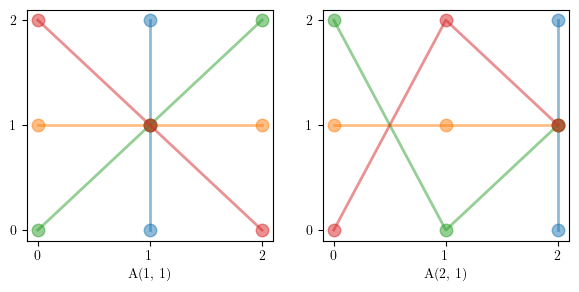
\includegraphics[width=0.9\textwidth]{imgs/As-3-1.png}
      \caption{Las rectas que pasan por los puntos $(1,1)$ y
      $(2,1)$ respectivamente.}
      \label{fig:point-lines-3-1}
    \end{figure}

    Para ilustrar el cálculo, vamos a construir el operador
    puntual correspondiente al origen. Como ya sabemos, las
    $3+1$ rectas que pasan por el origen son precisamente
    los rayos. Entonces, como hemos elegido asignar a los
    rayos del espacio de fase discreto, el operador de
    proyección del primer elemento de cada conjunto de
    vectores, un cálculo directo nos brinda
    \begin{equation}
      A(0,0)
      = \begin{pmatrix}
        1 & 0 & 0 \\
        0 & 0 & 1 \\
        0 & 1 & 0
      \end{pmatrix}. 
    \end{equation}
    Notemos que las propiedes 1 y 2 de
    (\ref{prop:point_props}) se satisfacen para éste
    operador puntual, ya que $A(0,0)$ es auto-adjunta y su
    traza es igual a $1$. En total existen $3^2 = 9$
    operadores puntuales para éste espacio de fase. Dado un
    operador de densidad $\rho$, su función de Wigner queda
    determinada como $W(x,y) = \frac{1}{3} \Tr(\rho
    A(x,y))$. Hemos gráficado la función de Wigner discreta
    para tres estados cuánticos:
    \begin{align}
      \ket{\psi_1}
      &= \ket 0 \\ 
      \ket{\psi_2}
      &= \frac{1}{\sqrt{3}}
      \left(
        \ket 0 + \omega \ket 1 + \omega \ket 2
      \right) \\
      \ket{\psi_3}
      &= \frac{1}{\sqrt{2}} (\ket 0 + \ket 1).
    \end{align}
    Los dos primeros estados cuánticos corresponden al
    primero vector de la primera base y al primer vector de
    la última base. El tercero es un vector arbitrario. La
    gráfica representa el espacio de fase discreto y el
    tamaño de la barra en el punto $(x,y)$ indica el valor
    de $W(x,y)$.

    \begin{figure}[ht]
      \centering
      \scalebox{0.7}{
        %% Creator: Matplotlib, PGF backend
%%
%% To include the figure in your LaTeX document, write
%%   \input{<filename>.pgf}
%%
%% Make sure the required packages are loaded in your preamble
%%   \usepackage{pgf}
%%
%% Also ensure that all the required font packages are loaded; for instance,
%% the lmodern package is sometimes necessary when using math font.
%%   \usepackage{lmodern}
%%
%% Figures using additional raster images can only be included by \input if
%% they are in the same directory as the main LaTeX file. For loading figures
%% from other directories you can use the `import` package
%%   \usepackage{import}
%%
%% and then include the figures with
%%   \import{<path to file>}{<filename>.pgf}
%%
%% Matplotlib used the following preamble
%%   
%%   \makeatletter\@ifpackageloaded{underscore}{}{\usepackage[strings]{underscore}}\makeatother
%%
\begingroup%
\makeatletter%
\begin{pgfpicture}%
\pgfpathrectangle{\pgfpointorigin}{\pgfqpoint{4.500000in}{3.500000in}}%
\pgfusepath{use as bounding box, clip}%
\begin{pgfscope}%
\pgfsetbuttcap%
\pgfsetmiterjoin%
\definecolor{currentfill}{rgb}{1.000000,1.000000,1.000000}%
\pgfsetfillcolor{currentfill}%
\pgfsetlinewidth{0.000000pt}%
\definecolor{currentstroke}{rgb}{1.000000,1.000000,1.000000}%
\pgfsetstrokecolor{currentstroke}%
\pgfsetdash{}{0pt}%
\pgfpathmoveto{\pgfqpoint{0.000000in}{0.000000in}}%
\pgfpathlineto{\pgfqpoint{4.500000in}{0.000000in}}%
\pgfpathlineto{\pgfqpoint{4.500000in}{3.500000in}}%
\pgfpathlineto{\pgfqpoint{0.000000in}{3.500000in}}%
\pgfpathlineto{\pgfqpoint{0.000000in}{0.000000in}}%
\pgfpathclose%
\pgfusepath{fill}%
\end{pgfscope}%
\begin{pgfscope}%
\pgfsetbuttcap%
\pgfsetmiterjoin%
\definecolor{currentfill}{rgb}{1.000000,1.000000,1.000000}%
\pgfsetfillcolor{currentfill}%
\pgfsetlinewidth{0.000000pt}%
\definecolor{currentstroke}{rgb}{0.000000,0.000000,0.000000}%
\pgfsetstrokecolor{currentstroke}%
\pgfsetstrokeopacity{0.000000}%
\pgfsetdash{}{0pt}%
\pgfpathmoveto{\pgfqpoint{0.562500in}{0.424687in}}%
\pgfpathlineto{\pgfqpoint{3.178125in}{0.424687in}}%
\pgfpathlineto{\pgfqpoint{3.178125in}{3.040313in}}%
\pgfpathlineto{\pgfqpoint{0.562500in}{3.040313in}}%
\pgfpathlineto{\pgfqpoint{0.562500in}{0.424687in}}%
\pgfpathclose%
\pgfusepath{fill}%
\end{pgfscope}%
\begin{pgfscope}%
\pgfsetbuttcap%
\pgfsetmiterjoin%
\definecolor{currentfill}{rgb}{0.950000,0.950000,0.950000}%
\pgfsetfillcolor{currentfill}%
\pgfsetfillopacity{0.500000}%
\pgfsetlinewidth{1.003750pt}%
\definecolor{currentstroke}{rgb}{0.950000,0.950000,0.950000}%
\pgfsetstrokecolor{currentstroke}%
\pgfsetstrokeopacity{0.500000}%
\pgfsetdash{}{0pt}%
\pgfpathmoveto{\pgfqpoint{0.776021in}{1.383786in}}%
\pgfpathlineto{\pgfqpoint{2.094656in}{1.909818in}}%
\pgfpathlineto{\pgfqpoint{2.103942in}{2.908896in}}%
\pgfpathlineto{\pgfqpoint{0.717370in}{2.412207in}}%
\pgfusepath{stroke,fill}%
\end{pgfscope}%
\begin{pgfscope}%
\pgfsetbuttcap%
\pgfsetmiterjoin%
\definecolor{currentfill}{rgb}{0.900000,0.900000,0.900000}%
\pgfsetfillcolor{currentfill}%
\pgfsetfillopacity{0.500000}%
\pgfsetlinewidth{1.003750pt}%
\definecolor{currentstroke}{rgb}{0.900000,0.900000,0.900000}%
\pgfsetstrokecolor{currentstroke}%
\pgfsetstrokeopacity{0.500000}%
\pgfsetdash{}{0pt}%
\pgfpathmoveto{\pgfqpoint{2.094656in}{1.909818in}}%
\pgfpathlineto{\pgfqpoint{3.061986in}{1.140817in}}%
\pgfpathlineto{\pgfqpoint{3.123516in}{2.181900in}}%
\pgfpathlineto{\pgfqpoint{2.103942in}{2.908896in}}%
\pgfusepath{stroke,fill}%
\end{pgfscope}%
\begin{pgfscope}%
\pgfsetbuttcap%
\pgfsetmiterjoin%
\definecolor{currentfill}{rgb}{0.925000,0.925000,0.925000}%
\pgfsetfillcolor{currentfill}%
\pgfsetfillopacity{0.500000}%
\pgfsetlinewidth{1.003750pt}%
\definecolor{currentstroke}{rgb}{0.925000,0.925000,0.925000}%
\pgfsetstrokecolor{currentstroke}%
\pgfsetstrokeopacity{0.500000}%
\pgfsetdash{}{0pt}%
\pgfpathmoveto{\pgfqpoint{0.776021in}{1.383786in}}%
\pgfpathlineto{\pgfqpoint{1.689859in}{0.525995in}}%
\pgfpathlineto{\pgfqpoint{3.061986in}{1.140817in}}%
\pgfpathlineto{\pgfqpoint{2.094656in}{1.909818in}}%
\pgfusepath{stroke,fill}%
\end{pgfscope}%
\begin{pgfscope}%
\pgfsetrectcap%
\pgfsetroundjoin%
\pgfsetlinewidth{0.803000pt}%
\definecolor{currentstroke}{rgb}{0.000000,0.000000,0.000000}%
\pgfsetstrokecolor{currentstroke}%
\pgfsetdash{}{0pt}%
\pgfpathmoveto{\pgfqpoint{0.776021in}{1.383786in}}%
\pgfpathlineto{\pgfqpoint{1.689859in}{0.525995in}}%
\pgfusepath{stroke}%
\end{pgfscope}%
\begin{pgfscope}%
\pgfsetbuttcap%
\pgfsetroundjoin%
\pgfsetlinewidth{0.803000pt}%
\definecolor{currentstroke}{rgb}{0.690196,0.690196,0.690196}%
\pgfsetstrokecolor{currentstroke}%
\pgfsetdash{}{0pt}%
\pgfpathmoveto{\pgfqpoint{0.964331in}{1.207025in}}%
\pgfpathlineto{\pgfqpoint{2.294663in}{1.750817in}}%
\pgfpathlineto{\pgfqpoint{2.314104in}{2.759043in}}%
\pgfusepath{stroke}%
\end{pgfscope}%
\begin{pgfscope}%
\pgfsetbuttcap%
\pgfsetroundjoin%
\pgfsetlinewidth{0.803000pt}%
\definecolor{currentstroke}{rgb}{0.690196,0.690196,0.690196}%
\pgfsetstrokecolor{currentstroke}%
\pgfsetdash{}{0pt}%
\pgfpathmoveto{\pgfqpoint{1.243156in}{0.945301in}}%
\pgfpathlineto{\pgfqpoint{2.590163in}{1.515903in}}%
\pgfpathlineto{\pgfqpoint{2.625223in}{2.537202in}}%
\pgfusepath{stroke}%
\end{pgfscope}%
\begin{pgfscope}%
\pgfsetbuttcap%
\pgfsetroundjoin%
\pgfsetlinewidth{0.803000pt}%
\definecolor{currentstroke}{rgb}{0.690196,0.690196,0.690196}%
\pgfsetstrokecolor{currentstroke}%
\pgfsetdash{}{0pt}%
\pgfpathmoveto{\pgfqpoint{1.536291in}{0.670145in}}%
\pgfpathlineto{\pgfqpoint{2.900003in}{1.269589in}}%
\pgfpathlineto{\pgfqpoint{2.952233in}{2.304032in}}%
\pgfusepath{stroke}%
\end{pgfscope}%
\begin{pgfscope}%
\pgfsetrectcap%
\pgfsetroundjoin%
\pgfsetlinewidth{0.803000pt}%
\definecolor{currentstroke}{rgb}{0.000000,0.000000,0.000000}%
\pgfsetstrokecolor{currentstroke}%
\pgfsetdash{}{0pt}%
\pgfpathmoveto{\pgfqpoint{0.975552in}{1.211612in}}%
\pgfpathlineto{\pgfqpoint{0.941859in}{1.197839in}}%
\pgfusepath{stroke}%
\end{pgfscope}%
\begin{pgfscope}%
\definecolor{textcolor}{rgb}{0.000000,0.000000,0.000000}%
\pgfsetstrokecolor{textcolor}%
\pgfsetfillcolor{textcolor}%
\pgftext[x=0.805259in,y=1.024118in,,top]{\color{textcolor}\rmfamily\fontsize{10.000000}{12.000000}\selectfont \(\displaystyle {0}\)}%
\end{pgfscope}%
\begin{pgfscope}%
\pgfsetrectcap%
\pgfsetroundjoin%
\pgfsetlinewidth{0.803000pt}%
\definecolor{currentstroke}{rgb}{0.000000,0.000000,0.000000}%
\pgfsetstrokecolor{currentstroke}%
\pgfsetdash{}{0pt}%
\pgfpathmoveto{\pgfqpoint{1.254532in}{0.950120in}}%
\pgfpathlineto{\pgfqpoint{1.220372in}{0.935650in}}%
\pgfusepath{stroke}%
\end{pgfscope}%
\begin{pgfscope}%
\definecolor{textcolor}{rgb}{0.000000,0.000000,0.000000}%
\pgfsetstrokecolor{textcolor}%
\pgfsetfillcolor{textcolor}%
\pgftext[x=1.080257in,y=0.757670in,,top]{\color{textcolor}\rmfamily\fontsize{10.000000}{12.000000}\selectfont \(\displaystyle {1}\)}%
\end{pgfscope}%
\begin{pgfscope}%
\pgfsetrectcap%
\pgfsetroundjoin%
\pgfsetlinewidth{0.803000pt}%
\definecolor{currentstroke}{rgb}{0.000000,0.000000,0.000000}%
\pgfsetstrokecolor{currentstroke}%
\pgfsetdash{}{0pt}%
\pgfpathmoveto{\pgfqpoint{1.547824in}{0.675214in}}%
\pgfpathlineto{\pgfqpoint{1.513192in}{0.659991in}}%
\pgfusepath{stroke}%
\end{pgfscope}%
\begin{pgfscope}%
\definecolor{textcolor}{rgb}{0.000000,0.000000,0.000000}%
\pgfsetstrokecolor{textcolor}%
\pgfsetfillcolor{textcolor}%
\pgftext[x=1.369377in,y=0.477539in,,top]{\color{textcolor}\rmfamily\fontsize{10.000000}{12.000000}\selectfont \(\displaystyle {2}\)}%
\end{pgfscope}%
\begin{pgfscope}%
\pgfsetrectcap%
\pgfsetroundjoin%
\pgfsetlinewidth{0.803000pt}%
\definecolor{currentstroke}{rgb}{0.000000,0.000000,0.000000}%
\pgfsetstrokecolor{currentstroke}%
\pgfsetdash{}{0pt}%
\pgfpathmoveto{\pgfqpoint{3.061986in}{1.140817in}}%
\pgfpathlineto{\pgfqpoint{1.689859in}{0.525995in}}%
\pgfusepath{stroke}%
\end{pgfscope}%
\begin{pgfscope}%
\pgfsetbuttcap%
\pgfsetroundjoin%
\pgfsetlinewidth{0.803000pt}%
\definecolor{currentstroke}{rgb}{0.690196,0.690196,0.690196}%
\pgfsetstrokecolor{currentstroke}%
\pgfsetdash{}{0pt}%
\pgfpathmoveto{\pgfqpoint{1.035000in}{2.525987in}}%
\pgfpathlineto{\pgfqpoint{1.077471in}{1.504040in}}%
\pgfpathlineto{\pgfqpoint{2.004569in}{0.667010in}}%
\pgfusepath{stroke}%
\end{pgfscope}%
\begin{pgfscope}%
\pgfsetbuttcap%
\pgfsetroundjoin%
\pgfsetlinewidth{0.803000pt}%
\definecolor{currentstroke}{rgb}{0.690196,0.690196,0.690196}%
\pgfsetstrokecolor{currentstroke}%
\pgfsetdash{}{0pt}%
\pgfpathmoveto{\pgfqpoint{1.472882in}{2.682842in}}%
\pgfpathlineto{\pgfqpoint{1.493648in}{1.670063in}}%
\pgfpathlineto{\pgfqpoint{2.438046in}{0.861242in}}%
\pgfusepath{stroke}%
\end{pgfscope}%
\begin{pgfscope}%
\pgfsetbuttcap%
\pgfsetroundjoin%
\pgfsetlinewidth{0.803000pt}%
\definecolor{currentstroke}{rgb}{0.690196,0.690196,0.690196}%
\pgfsetstrokecolor{currentstroke}%
\pgfsetdash{}{0pt}%
\pgfpathmoveto{\pgfqpoint{1.895991in}{2.834405in}}%
\pgfpathlineto{\pgfqpoint{1.896448in}{1.830748in}}%
\pgfpathlineto{\pgfqpoint{2.856482in}{1.048735in}}%
\pgfusepath{stroke}%
\end{pgfscope}%
\begin{pgfscope}%
\pgfsetrectcap%
\pgfsetroundjoin%
\pgfsetlinewidth{0.803000pt}%
\definecolor{currentstroke}{rgb}{0.000000,0.000000,0.000000}%
\pgfsetstrokecolor{currentstroke}%
\pgfsetdash{}{0pt}%
\pgfpathmoveto{\pgfqpoint{1.996546in}{0.674253in}}%
\pgfpathlineto{\pgfqpoint{2.020645in}{0.652495in}}%
\pgfusepath{stroke}%
\end{pgfscope}%
\begin{pgfscope}%
\definecolor{textcolor}{rgb}{0.000000,0.000000,0.000000}%
\pgfsetstrokecolor{textcolor}%
\pgfsetfillcolor{textcolor}%
\pgftext[x=2.122012in,y=0.441833in,,top]{\color{textcolor}\rmfamily\fontsize{10.000000}{12.000000}\selectfont \(\displaystyle {0}\)}%
\end{pgfscope}%
\begin{pgfscope}%
\pgfsetrectcap%
\pgfsetroundjoin%
\pgfsetlinewidth{0.803000pt}%
\definecolor{currentstroke}{rgb}{0.000000,0.000000,0.000000}%
\pgfsetstrokecolor{currentstroke}%
\pgfsetdash{}{0pt}%
\pgfpathmoveto{\pgfqpoint{2.429885in}{0.868232in}}%
\pgfpathlineto{\pgfqpoint{2.454400in}{0.847236in}}%
\pgfusepath{stroke}%
\end{pgfscope}%
\begin{pgfscope}%
\definecolor{textcolor}{rgb}{0.000000,0.000000,0.000000}%
\pgfsetstrokecolor{textcolor}%
\pgfsetfillcolor{textcolor}%
\pgftext[x=2.554889in,y=0.640719in,,top]{\color{textcolor}\rmfamily\fontsize{10.000000}{12.000000}\selectfont \(\displaystyle {1}\)}%
\end{pgfscope}%
\begin{pgfscope}%
\pgfsetrectcap%
\pgfsetroundjoin%
\pgfsetlinewidth{0.803000pt}%
\definecolor{currentstroke}{rgb}{0.000000,0.000000,0.000000}%
\pgfsetstrokecolor{currentstroke}%
\pgfsetdash{}{0pt}%
\pgfpathmoveto{\pgfqpoint{2.848196in}{1.055484in}}%
\pgfpathlineto{\pgfqpoint{2.873085in}{1.035211in}}%
\pgfusepath{stroke}%
\end{pgfscope}%
\begin{pgfscope}%
\definecolor{textcolor}{rgb}{0.000000,0.000000,0.000000}%
\pgfsetstrokecolor{textcolor}%
\pgfsetfillcolor{textcolor}%
\pgftext[x=2.972696in,y=0.832679in,,top]{\color{textcolor}\rmfamily\fontsize{10.000000}{12.000000}\selectfont \(\displaystyle {2}\)}%
\end{pgfscope}%
\begin{pgfscope}%
\pgfsetrectcap%
\pgfsetroundjoin%
\pgfsetlinewidth{0.803000pt}%
\definecolor{currentstroke}{rgb}{0.000000,0.000000,0.000000}%
\pgfsetstrokecolor{currentstroke}%
\pgfsetdash{}{0pt}%
\pgfpathmoveto{\pgfqpoint{3.061986in}{1.140817in}}%
\pgfpathlineto{\pgfqpoint{3.123516in}{2.181900in}}%
\pgfusepath{stroke}%
\end{pgfscope}%
\begin{pgfscope}%
\pgfpathrectangle{\pgfqpoint{0.562500in}{0.424687in}}{\pgfqpoint{2.615625in}{2.615625in}}%
\pgfusepath{clip}%
\pgfsetbuttcap%
\pgfsetroundjoin%
\definecolor{currentfill}{rgb}{0.529732,0.483284,0.076766}%
\pgfsetfillcolor{currentfill}%
\pgfsetlinewidth{0.000000pt}%
\definecolor{currentstroke}{rgb}{0.000000,0.000000,0.000000}%
\pgfsetstrokecolor{currentstroke}%
\pgfsetdash{}{0pt}%
\pgfpathmoveto{\pgfqpoint{1.752909in}{1.723253in}}%
\pgfpathlineto{\pgfqpoint{2.072073in}{1.851221in}}%
\pgfpathlineto{\pgfqpoint{2.301452in}{1.667438in}}%
\pgfpathlineto{\pgfqpoint{1.979279in}{1.534602in}}%
\pgfpathlineto{\pgfqpoint{1.752909in}{1.723253in}}%
\pgfpathclose%
\pgfusepath{fill}%
\end{pgfscope}%
\begin{pgfscope}%
\pgfpathrectangle{\pgfqpoint{0.562500in}{0.424687in}}{\pgfqpoint{2.615625in}{2.615625in}}%
\pgfusepath{clip}%
\pgfsetbuttcap%
\pgfsetroundjoin%
\definecolor{currentfill}{rgb}{0.111252,0.002031,0.137256}%
\pgfsetfillcolor{currentfill}%
\pgfsetlinewidth{0.000000pt}%
\definecolor{currentstroke}{rgb}{0.000000,0.000000,0.000000}%
\pgfsetstrokecolor{currentstroke}%
\pgfsetdash{}{0pt}%
\pgfpathmoveto{\pgfqpoint{2.037221in}{1.486315in}}%
\pgfpathlineto{\pgfqpoint{2.037221in}{1.486315in}}%
\pgfpathlineto{\pgfqpoint{2.360145in}{1.620412in}}%
\pgfpathlineto{\pgfqpoint{2.360145in}{1.620412in}}%
\pgfpathlineto{\pgfqpoint{2.037221in}{1.486315in}}%
\pgfpathclose%
\pgfusepath{fill}%
\end{pgfscope}%
\begin{pgfscope}%
\pgfpathrectangle{\pgfqpoint{0.562500in}{0.424687in}}{\pgfqpoint{2.615625in}{2.615625in}}%
\pgfusepath{clip}%
\pgfsetbuttcap%
\pgfsetroundjoin%
\definecolor{currentfill}{rgb}{0.877369,0.800439,0.127143}%
\pgfsetfillcolor{currentfill}%
\pgfsetlinewidth{0.000000pt}%
\definecolor{currentstroke}{rgb}{0.000000,0.000000,0.000000}%
\pgfsetstrokecolor{currentstroke}%
\pgfsetdash{}{0pt}%
\pgfpathmoveto{\pgfqpoint{1.752909in}{1.723253in}}%
\pgfpathlineto{\pgfqpoint{1.745551in}{2.693647in}}%
\pgfpathlineto{\pgfqpoint{2.079980in}{2.814615in}}%
\pgfpathlineto{\pgfqpoint{2.072073in}{1.851221in}}%
\pgfpathlineto{\pgfqpoint{1.752909in}{1.723253in}}%
\pgfpathclose%
\pgfusepath{fill}%
\end{pgfscope}%
\begin{pgfscope}%
\pgfpathrectangle{\pgfqpoint{0.562500in}{0.424687in}}{\pgfqpoint{2.615625in}{2.615625in}}%
\pgfusepath{clip}%
\pgfsetbuttcap%
\pgfsetroundjoin%
\definecolor{currentfill}{rgb}{0.529732,0.483284,0.076766}%
\pgfsetfillcolor{currentfill}%
\pgfsetlinewidth{0.000000pt}%
\definecolor{currentstroke}{rgb}{0.000000,0.000000,0.000000}%
\pgfsetstrokecolor{currentstroke}%
\pgfsetdash{}{0pt}%
\pgfpathmoveto{\pgfqpoint{1.342057in}{1.558524in}}%
\pgfpathlineto{\pgfqpoint{1.671813in}{1.690738in}}%
\pgfpathlineto{\pgfqpoint{1.897395in}{1.500839in}}%
\pgfpathlineto{\pgfqpoint{1.564325in}{1.363509in}}%
\pgfpathlineto{\pgfqpoint{1.342057in}{1.558524in}}%
\pgfpathclose%
\pgfusepath{fill}%
\end{pgfscope}%
\begin{pgfscope}%
\pgfpathrectangle{\pgfqpoint{0.562500in}{0.424687in}}{\pgfqpoint{2.615625in}{2.615625in}}%
\pgfusepath{clip}%
\pgfsetbuttcap%
\pgfsetroundjoin%
\definecolor{currentfill}{rgb}{0.235854,0.004305,0.290983}%
\pgfsetfillcolor{currentfill}%
\pgfsetlinewidth{0.000000pt}%
\definecolor{currentstroke}{rgb}{0.000000,0.000000,0.000000}%
\pgfsetstrokecolor{currentstroke}%
\pgfsetdash{}{0pt}%
\pgfpathmoveto{\pgfqpoint{2.360145in}{1.620412in}}%
\pgfpathlineto{\pgfqpoint{2.360145in}{1.620412in}}%
\pgfpathlineto{\pgfqpoint{2.600542in}{1.427801in}}%
\pgfpathlineto{\pgfqpoint{2.600542in}{1.427801in}}%
\pgfpathlineto{\pgfqpoint{2.360145in}{1.620412in}}%
\pgfpathclose%
\pgfusepath{fill}%
\end{pgfscope}%
\begin{pgfscope}%
\pgfpathrectangle{\pgfqpoint{0.562500in}{0.424687in}}{\pgfqpoint{2.615625in}{2.615625in}}%
\pgfusepath{clip}%
\pgfsetbuttcap%
\pgfsetroundjoin%
\definecolor{currentfill}{rgb}{0.413853,0.377565,0.059973}%
\pgfsetfillcolor{currentfill}%
\pgfsetlinewidth{0.000000pt}%
\definecolor{currentstroke}{rgb}{0.000000,0.000000,0.000000}%
\pgfsetstrokecolor{currentstroke}%
\pgfsetdash{}{0pt}%
\pgfpathmoveto{\pgfqpoint{2.072073in}{1.851221in}}%
\pgfpathlineto{\pgfqpoint{2.079980in}{2.814615in}}%
\pgfpathlineto{\pgfqpoint{2.320627in}{2.640838in}}%
\pgfpathlineto{\pgfqpoint{2.301452in}{1.667438in}}%
\pgfpathlineto{\pgfqpoint{2.072073in}{1.851221in}}%
\pgfpathclose%
\pgfusepath{fill}%
\end{pgfscope}%
\begin{pgfscope}%
\pgfpathrectangle{\pgfqpoint{0.562500in}{0.424687in}}{\pgfqpoint{2.615625in}{2.615625in}}%
\pgfusepath{clip}%
\pgfsetbuttcap%
\pgfsetroundjoin%
\definecolor{currentfill}{rgb}{0.204703,0.003737,0.252551}%
\pgfsetfillcolor{currentfill}%
\pgfsetlinewidth{0.000000pt}%
\definecolor{currentstroke}{rgb}{0.000000,0.000000,0.000000}%
\pgfsetstrokecolor{currentstroke}%
\pgfsetdash{}{0pt}%
\pgfpathmoveto{\pgfqpoint{2.037221in}{1.486315in}}%
\pgfpathlineto{\pgfqpoint{2.274614in}{1.288477in}}%
\pgfpathlineto{\pgfqpoint{2.600542in}{1.427801in}}%
\pgfpathlineto{\pgfqpoint{2.360145in}{1.620412in}}%
\pgfpathlineto{\pgfqpoint{2.037221in}{1.486315in}}%
\pgfpathclose%
\pgfusepath{fill}%
\end{pgfscope}%
\begin{pgfscope}%
\pgfpathrectangle{\pgfqpoint{0.562500in}{0.424687in}}{\pgfqpoint{2.615625in}{2.615625in}}%
\pgfusepath{clip}%
\pgfsetbuttcap%
\pgfsetroundjoin%
\definecolor{currentfill}{rgb}{0.142402,0.002599,0.175688}%
\pgfsetfillcolor{currentfill}%
\pgfsetlinewidth{0.000000pt}%
\definecolor{currentstroke}{rgb}{0.000000,0.000000,0.000000}%
\pgfsetstrokecolor{currentstroke}%
\pgfsetdash{}{0pt}%
\pgfpathmoveto{\pgfqpoint{2.037221in}{1.486315in}}%
\pgfpathlineto{\pgfqpoint{2.360145in}{1.620412in}}%
\pgfpathlineto{\pgfqpoint{2.600542in}{1.427801in}}%
\pgfpathlineto{\pgfqpoint{2.274614in}{1.288477in}}%
\pgfpathlineto{\pgfqpoint{2.037221in}{1.486315in}}%
\pgfpathclose%
\pgfusepath{fill}%
\end{pgfscope}%
\begin{pgfscope}%
\pgfpathrectangle{\pgfqpoint{0.562500in}{0.424687in}}{\pgfqpoint{2.615625in}{2.615625in}}%
\pgfusepath{clip}%
\pgfsetbuttcap%
\pgfsetroundjoin%
\definecolor{currentfill}{rgb}{0.111252,0.002031,0.137256}%
\pgfsetfillcolor{currentfill}%
\pgfsetlinewidth{0.000000pt}%
\definecolor{currentstroke}{rgb}{0.000000,0.000000,0.000000}%
\pgfsetstrokecolor{currentstroke}%
\pgfsetdash{}{0pt}%
\pgfpathmoveto{\pgfqpoint{2.037221in}{1.486315in}}%
\pgfpathlineto{\pgfqpoint{2.274614in}{1.288477in}}%
\pgfpathlineto{\pgfqpoint{2.274614in}{1.288477in}}%
\pgfpathlineto{\pgfqpoint{2.037221in}{1.486315in}}%
\pgfpathlineto{\pgfqpoint{2.037221in}{1.486315in}}%
\pgfpathclose%
\pgfusepath{fill}%
\end{pgfscope}%
\begin{pgfscope}%
\pgfpathrectangle{\pgfqpoint{0.562500in}{0.424687in}}{\pgfqpoint{2.615625in}{2.615625in}}%
\pgfusepath{clip}%
\pgfsetbuttcap%
\pgfsetroundjoin%
\definecolor{currentfill}{rgb}{0.877369,0.800439,0.127143}%
\pgfsetfillcolor{currentfill}%
\pgfsetlinewidth{0.000000pt}%
\definecolor{currentstroke}{rgb}{0.000000,0.000000,0.000000}%
\pgfsetstrokecolor{currentstroke}%
\pgfsetdash{}{0pt}%
\pgfpathmoveto{\pgfqpoint{1.752909in}{1.723253in}}%
\pgfpathlineto{\pgfqpoint{1.979279in}{1.534602in}}%
\pgfpathlineto{\pgfqpoint{1.982896in}{2.515041in}}%
\pgfpathlineto{\pgfqpoint{1.745551in}{2.693647in}}%
\pgfpathlineto{\pgfqpoint{1.752909in}{1.723253in}}%
\pgfpathclose%
\pgfusepath{fill}%
\end{pgfscope}%
\begin{pgfscope}%
\pgfpathrectangle{\pgfqpoint{0.562500in}{0.424687in}}{\pgfqpoint{2.615625in}{2.615625in}}%
\pgfusepath{clip}%
\pgfsetbuttcap%
\pgfsetroundjoin%
\definecolor{currentfill}{rgb}{0.111252,0.002031,0.137256}%
\pgfsetfillcolor{currentfill}%
\pgfsetlinewidth{0.000000pt}%
\definecolor{currentstroke}{rgb}{0.000000,0.000000,0.000000}%
\pgfsetstrokecolor{currentstroke}%
\pgfsetdash{}{0pt}%
\pgfpathmoveto{\pgfqpoint{1.621238in}{1.313574in}}%
\pgfpathlineto{\pgfqpoint{1.621238in}{1.313574in}}%
\pgfpathlineto{\pgfqpoint{1.955138in}{1.452229in}}%
\pgfpathlineto{\pgfqpoint{1.955138in}{1.452229in}}%
\pgfpathlineto{\pgfqpoint{1.621238in}{1.313574in}}%
\pgfpathclose%
\pgfusepath{fill}%
\end{pgfscope}%
\begin{pgfscope}%
\pgfpathrectangle{\pgfqpoint{0.562500in}{0.424687in}}{\pgfqpoint{2.615625in}{2.615625in}}%
\pgfusepath{clip}%
\pgfsetbuttcap%
\pgfsetroundjoin%
\definecolor{currentfill}{rgb}{0.877369,0.800439,0.127143}%
\pgfsetfillcolor{currentfill}%
\pgfsetlinewidth{0.000000pt}%
\definecolor{currentstroke}{rgb}{0.000000,0.000000,0.000000}%
\pgfsetstrokecolor{currentstroke}%
\pgfsetdash{}{0pt}%
\pgfpathmoveto{\pgfqpoint{1.342057in}{1.558524in}}%
\pgfpathlineto{\pgfqpoint{1.314440in}{2.537707in}}%
\pgfpathlineto{\pgfqpoint{1.660511in}{2.662886in}}%
\pgfpathlineto{\pgfqpoint{1.671813in}{1.690738in}}%
\pgfpathlineto{\pgfqpoint{1.342057in}{1.558524in}}%
\pgfpathclose%
\pgfusepath{fill}%
\end{pgfscope}%
\begin{pgfscope}%
\pgfpathrectangle{\pgfqpoint{0.562500in}{0.424687in}}{\pgfqpoint{2.615625in}{2.615625in}}%
\pgfusepath{clip}%
\pgfsetbuttcap%
\pgfsetroundjoin%
\definecolor{currentfill}{rgb}{0.235854,0.004305,0.290983}%
\pgfsetfillcolor{currentfill}%
\pgfsetlinewidth{0.000000pt}%
\definecolor{currentstroke}{rgb}{0.000000,0.000000,0.000000}%
\pgfsetstrokecolor{currentstroke}%
\pgfsetdash{}{0pt}%
\pgfpathmoveto{\pgfqpoint{2.274614in}{1.288477in}}%
\pgfpathlineto{\pgfqpoint{2.600542in}{1.427801in}}%
\pgfpathlineto{\pgfqpoint{2.600542in}{1.427801in}}%
\pgfpathlineto{\pgfqpoint{2.274614in}{1.288477in}}%
\pgfpathlineto{\pgfqpoint{2.274614in}{1.288477in}}%
\pgfpathclose%
\pgfusepath{fill}%
\end{pgfscope}%
\begin{pgfscope}%
\pgfpathrectangle{\pgfqpoint{0.562500in}{0.424687in}}{\pgfqpoint{2.615625in}{2.615625in}}%
\pgfusepath{clip}%
\pgfsetbuttcap%
\pgfsetroundjoin%
\definecolor{currentfill}{rgb}{0.529732,0.483284,0.076766}%
\pgfsetfillcolor{currentfill}%
\pgfsetlinewidth{0.000000pt}%
\definecolor{currentstroke}{rgb}{0.000000,0.000000,0.000000}%
\pgfsetstrokecolor{currentstroke}%
\pgfsetdash{}{0pt}%
\pgfpathmoveto{\pgfqpoint{0.917366in}{1.388245in}}%
\pgfpathlineto{\pgfqpoint{1.258248in}{1.524921in}}%
\pgfpathlineto{\pgfqpoint{1.479647in}{1.328595in}}%
\pgfpathlineto{\pgfqpoint{1.135117in}{1.186540in}}%
\pgfpathlineto{\pgfqpoint{0.917366in}{1.388245in}}%
\pgfpathclose%
\pgfusepath{fill}%
\end{pgfscope}%
\begin{pgfscope}%
\pgfpathrectangle{\pgfqpoint{0.562500in}{0.424687in}}{\pgfqpoint{2.615625in}{2.615625in}}%
\pgfusepath{clip}%
\pgfsetbuttcap%
\pgfsetroundjoin%
\definecolor{currentfill}{rgb}{0.413853,0.377565,0.059973}%
\pgfsetfillcolor{currentfill}%
\pgfsetlinewidth{0.000000pt}%
\definecolor{currentstroke}{rgb}{0.000000,0.000000,0.000000}%
\pgfsetstrokecolor{currentstroke}%
\pgfsetdash{}{0pt}%
\pgfpathmoveto{\pgfqpoint{1.979279in}{1.534602in}}%
\pgfpathlineto{\pgfqpoint{2.301452in}{1.667438in}}%
\pgfpathlineto{\pgfqpoint{2.320627in}{2.640838in}}%
\pgfpathlineto{\pgfqpoint{1.982896in}{2.515041in}}%
\pgfpathlineto{\pgfqpoint{1.979279in}{1.534602in}}%
\pgfpathclose%
\pgfusepath{fill}%
\end{pgfscope}%
\begin{pgfscope}%
\pgfpathrectangle{\pgfqpoint{0.562500in}{0.424687in}}{\pgfqpoint{2.615625in}{2.615625in}}%
\pgfusepath{clip}%
\pgfsetbuttcap%
\pgfsetroundjoin%
\definecolor{currentfill}{rgb}{0.235854,0.004305,0.290983}%
\pgfsetfillcolor{currentfill}%
\pgfsetlinewidth{0.000000pt}%
\definecolor{currentstroke}{rgb}{0.000000,0.000000,0.000000}%
\pgfsetstrokecolor{currentstroke}%
\pgfsetdash{}{0pt}%
\pgfpathmoveto{\pgfqpoint{1.955138in}{1.452229in}}%
\pgfpathlineto{\pgfqpoint{1.955138in}{1.452229in}}%
\pgfpathlineto{\pgfqpoint{2.191742in}{1.253051in}}%
\pgfpathlineto{\pgfqpoint{2.191742in}{1.253052in}}%
\pgfpathlineto{\pgfqpoint{1.955138in}{1.452229in}}%
\pgfpathclose%
\pgfusepath{fill}%
\end{pgfscope}%
\begin{pgfscope}%
\pgfpathrectangle{\pgfqpoint{0.562500in}{0.424687in}}{\pgfqpoint{2.615625in}{2.615625in}}%
\pgfusepath{clip}%
\pgfsetbuttcap%
\pgfsetroundjoin%
\definecolor{currentfill}{rgb}{0.413853,0.377565,0.059973}%
\pgfsetfillcolor{currentfill}%
\pgfsetlinewidth{0.000000pt}%
\definecolor{currentstroke}{rgb}{0.000000,0.000000,0.000000}%
\pgfsetstrokecolor{currentstroke}%
\pgfsetdash{}{0pt}%
\pgfpathmoveto{\pgfqpoint{1.671813in}{1.690738in}}%
\pgfpathlineto{\pgfqpoint{1.660511in}{2.662886in}}%
\pgfpathlineto{\pgfqpoint{1.896987in}{2.483042in}}%
\pgfpathlineto{\pgfqpoint{1.897395in}{1.500839in}}%
\pgfpathlineto{\pgfqpoint{1.671813in}{1.690738in}}%
\pgfpathclose%
\pgfusepath{fill}%
\end{pgfscope}%
\begin{pgfscope}%
\pgfpathrectangle{\pgfqpoint{0.562500in}{0.424687in}}{\pgfqpoint{2.615625in}{2.615625in}}%
\pgfusepath{clip}%
\pgfsetbuttcap%
\pgfsetroundjoin%
\definecolor{currentfill}{rgb}{0.111252,0.002031,0.137256}%
\pgfsetfillcolor{currentfill}%
\pgfsetlinewidth{0.000000pt}%
\definecolor{currentstroke}{rgb}{0.000000,0.000000,0.000000}%
\pgfsetstrokecolor{currentstroke}%
\pgfsetdash{}{0pt}%
\pgfpathmoveto{\pgfqpoint{2.335411in}{1.237810in}}%
\pgfpathlineto{\pgfqpoint{2.335411in}{1.237810in}}%
\pgfpathlineto{\pgfqpoint{2.662089in}{1.378488in}}%
\pgfpathlineto{\pgfqpoint{2.662089in}{1.378488in}}%
\pgfpathlineto{\pgfqpoint{2.335411in}{1.237810in}}%
\pgfpathclose%
\pgfusepath{fill}%
\end{pgfscope}%
\begin{pgfscope}%
\pgfpathrectangle{\pgfqpoint{0.562500in}{0.424687in}}{\pgfqpoint{2.615625in}{2.615625in}}%
\pgfusepath{clip}%
\pgfsetbuttcap%
\pgfsetroundjoin%
\definecolor{currentfill}{rgb}{0.204703,0.003737,0.252551}%
\pgfsetfillcolor{currentfill}%
\pgfsetlinewidth{0.000000pt}%
\definecolor{currentstroke}{rgb}{0.000000,0.000000,0.000000}%
\pgfsetstrokecolor{currentstroke}%
\pgfsetdash{}{0pt}%
\pgfpathmoveto{\pgfqpoint{1.621238in}{1.313574in}}%
\pgfpathlineto{\pgfqpoint{1.854516in}{1.108898in}}%
\pgfpathlineto{\pgfqpoint{2.191742in}{1.253051in}}%
\pgfpathlineto{\pgfqpoint{1.955138in}{1.452229in}}%
\pgfpathlineto{\pgfqpoint{1.621238in}{1.313574in}}%
\pgfpathclose%
\pgfusepath{fill}%
\end{pgfscope}%
\begin{pgfscope}%
\pgfpathrectangle{\pgfqpoint{0.562500in}{0.424687in}}{\pgfqpoint{2.615625in}{2.615625in}}%
\pgfusepath{clip}%
\pgfsetbuttcap%
\pgfsetroundjoin%
\definecolor{currentfill}{rgb}{0.142402,0.002599,0.175688}%
\pgfsetfillcolor{currentfill}%
\pgfsetlinewidth{0.000000pt}%
\definecolor{currentstroke}{rgb}{0.000000,0.000000,0.000000}%
\pgfsetstrokecolor{currentstroke}%
\pgfsetdash{}{0pt}%
\pgfpathmoveto{\pgfqpoint{1.621238in}{1.313574in}}%
\pgfpathlineto{\pgfqpoint{1.955138in}{1.452229in}}%
\pgfpathlineto{\pgfqpoint{2.191742in}{1.253052in}}%
\pgfpathlineto{\pgfqpoint{1.854516in}{1.108898in}}%
\pgfpathlineto{\pgfqpoint{1.621238in}{1.313574in}}%
\pgfpathclose%
\pgfusepath{fill}%
\end{pgfscope}%
\begin{pgfscope}%
\pgfpathrectangle{\pgfqpoint{0.562500in}{0.424687in}}{\pgfqpoint{2.615625in}{2.615625in}}%
\pgfusepath{clip}%
\pgfsetbuttcap%
\pgfsetroundjoin%
\definecolor{currentfill}{rgb}{0.235854,0.004305,0.290983}%
\pgfsetfillcolor{currentfill}%
\pgfsetlinewidth{0.000000pt}%
\definecolor{currentstroke}{rgb}{0.000000,0.000000,0.000000}%
\pgfsetstrokecolor{currentstroke}%
\pgfsetdash{}{0pt}%
\pgfpathmoveto{\pgfqpoint{2.662089in}{1.378488in}}%
\pgfpathlineto{\pgfqpoint{2.662089in}{1.378488in}}%
\pgfpathlineto{\pgfqpoint{2.914319in}{1.176396in}}%
\pgfpathlineto{\pgfqpoint{2.914319in}{1.176396in}}%
\pgfpathlineto{\pgfqpoint{2.662089in}{1.378488in}}%
\pgfpathclose%
\pgfusepath{fill}%
\end{pgfscope}%
\begin{pgfscope}%
\pgfpathrectangle{\pgfqpoint{0.562500in}{0.424687in}}{\pgfqpoint{2.615625in}{2.615625in}}%
\pgfusepath{clip}%
\pgfsetbuttcap%
\pgfsetroundjoin%
\definecolor{currentfill}{rgb}{0.761490,0.694720,0.110351}%
\pgfsetfillcolor{currentfill}%
\pgfsetlinewidth{0.000000pt}%
\definecolor{currentstroke}{rgb}{0.000000,0.000000,0.000000}%
\pgfsetstrokecolor{currentstroke}%
\pgfsetdash{}{0pt}%
\pgfpathmoveto{\pgfqpoint{1.745551in}{2.693647in}}%
\pgfpathlineto{\pgfqpoint{1.982896in}{2.515041in}}%
\pgfpathlineto{\pgfqpoint{2.320627in}{2.640838in}}%
\pgfpathlineto{\pgfqpoint{2.079980in}{2.814615in}}%
\pgfpathlineto{\pgfqpoint{1.745551in}{2.693647in}}%
\pgfpathclose%
\pgfusepath{fill}%
\end{pgfscope}%
\begin{pgfscope}%
\pgfpathrectangle{\pgfqpoint{0.562500in}{0.424687in}}{\pgfqpoint{2.615625in}{2.615625in}}%
\pgfusepath{clip}%
\pgfsetbuttcap%
\pgfsetroundjoin%
\definecolor{currentfill}{rgb}{0.111252,0.002031,0.137256}%
\pgfsetfillcolor{currentfill}%
\pgfsetlinewidth{0.000000pt}%
\definecolor{currentstroke}{rgb}{0.000000,0.000000,0.000000}%
\pgfsetstrokecolor{currentstroke}%
\pgfsetdash{}{0pt}%
\pgfpathmoveto{\pgfqpoint{1.621238in}{1.313574in}}%
\pgfpathlineto{\pgfqpoint{1.854516in}{1.108898in}}%
\pgfpathlineto{\pgfqpoint{1.854516in}{1.108898in}}%
\pgfpathlineto{\pgfqpoint{1.621238in}{1.313574in}}%
\pgfpathlineto{\pgfqpoint{1.621238in}{1.313574in}}%
\pgfpathclose%
\pgfusepath{fill}%
\end{pgfscope}%
\begin{pgfscope}%
\pgfpathrectangle{\pgfqpoint{0.562500in}{0.424687in}}{\pgfqpoint{2.615625in}{2.615625in}}%
\pgfusepath{clip}%
\pgfsetbuttcap%
\pgfsetroundjoin%
\definecolor{currentfill}{rgb}{0.877369,0.800439,0.127143}%
\pgfsetfillcolor{currentfill}%
\pgfsetlinewidth{0.000000pt}%
\definecolor{currentstroke}{rgb}{0.000000,0.000000,0.000000}%
\pgfsetstrokecolor{currentstroke}%
\pgfsetdash{}{0pt}%
\pgfpathmoveto{\pgfqpoint{1.342057in}{1.558524in}}%
\pgfpathlineto{\pgfqpoint{1.564325in}{1.363509in}}%
\pgfpathlineto{\pgfqpoint{1.547260in}{2.352776in}}%
\pgfpathlineto{\pgfqpoint{1.314440in}{2.537707in}}%
\pgfpathlineto{\pgfqpoint{1.342057in}{1.558524in}}%
\pgfpathclose%
\pgfusepath{fill}%
\end{pgfscope}%
\begin{pgfscope}%
\pgfpathrectangle{\pgfqpoint{0.562500in}{0.424687in}}{\pgfqpoint{2.615625in}{2.615625in}}%
\pgfusepath{clip}%
\pgfsetbuttcap%
\pgfsetroundjoin%
\definecolor{currentfill}{rgb}{0.111252,0.002031,0.137256}%
\pgfsetfillcolor{currentfill}%
\pgfsetlinewidth{0.000000pt}%
\definecolor{currentstroke}{rgb}{0.000000,0.000000,0.000000}%
\pgfsetstrokecolor{currentstroke}%
\pgfsetdash{}{0pt}%
\pgfpathmoveto{\pgfqpoint{1.190897in}{1.134870in}}%
\pgfpathlineto{\pgfqpoint{1.190897in}{1.134870in}}%
\pgfpathlineto{\pgfqpoint{1.536342in}{1.278320in}}%
\pgfpathlineto{\pgfqpoint{1.536342in}{1.278320in}}%
\pgfpathlineto{\pgfqpoint{1.190897in}{1.134870in}}%
\pgfpathclose%
\pgfusepath{fill}%
\end{pgfscope}%
\begin{pgfscope}%
\pgfpathrectangle{\pgfqpoint{0.562500in}{0.424687in}}{\pgfqpoint{2.615625in}{2.615625in}}%
\pgfusepath{clip}%
\pgfsetbuttcap%
\pgfsetroundjoin%
\definecolor{currentfill}{rgb}{0.204703,0.003737,0.252551}%
\pgfsetfillcolor{currentfill}%
\pgfsetlinewidth{0.000000pt}%
\definecolor{currentstroke}{rgb}{0.000000,0.000000,0.000000}%
\pgfsetstrokecolor{currentstroke}%
\pgfsetdash{}{0pt}%
\pgfpathmoveto{\pgfqpoint{2.335411in}{1.237810in}}%
\pgfpathlineto{\pgfqpoint{2.584653in}{1.030098in}}%
\pgfpathlineto{\pgfqpoint{2.914319in}{1.176396in}}%
\pgfpathlineto{\pgfqpoint{2.662089in}{1.378488in}}%
\pgfpathlineto{\pgfqpoint{2.335411in}{1.237810in}}%
\pgfpathclose%
\pgfusepath{fill}%
\end{pgfscope}%
\begin{pgfscope}%
\pgfpathrectangle{\pgfqpoint{0.562500in}{0.424687in}}{\pgfqpoint{2.615625in}{2.615625in}}%
\pgfusepath{clip}%
\pgfsetbuttcap%
\pgfsetroundjoin%
\definecolor{currentfill}{rgb}{0.142402,0.002599,0.175688}%
\pgfsetfillcolor{currentfill}%
\pgfsetlinewidth{0.000000pt}%
\definecolor{currentstroke}{rgb}{0.000000,0.000000,0.000000}%
\pgfsetstrokecolor{currentstroke}%
\pgfsetdash{}{0pt}%
\pgfpathmoveto{\pgfqpoint{2.335411in}{1.237810in}}%
\pgfpathlineto{\pgfqpoint{2.662089in}{1.378488in}}%
\pgfpathlineto{\pgfqpoint{2.914319in}{1.176396in}}%
\pgfpathlineto{\pgfqpoint{2.584653in}{1.030098in}}%
\pgfpathlineto{\pgfqpoint{2.335411in}{1.237810in}}%
\pgfpathclose%
\pgfusepath{fill}%
\end{pgfscope}%
\begin{pgfscope}%
\pgfpathrectangle{\pgfqpoint{0.562500in}{0.424687in}}{\pgfqpoint{2.615625in}{2.615625in}}%
\pgfusepath{clip}%
\pgfsetbuttcap%
\pgfsetroundjoin%
\definecolor{currentfill}{rgb}{0.877369,0.800439,0.127143}%
\pgfsetfillcolor{currentfill}%
\pgfsetlinewidth{0.000000pt}%
\definecolor{currentstroke}{rgb}{0.000000,0.000000,0.000000}%
\pgfsetstrokecolor{currentstroke}%
\pgfsetdash{}{0pt}%
\pgfpathmoveto{\pgfqpoint{0.917366in}{1.388245in}}%
\pgfpathlineto{\pgfqpoint{0.868081in}{2.376253in}}%
\pgfpathlineto{\pgfqpoint{1.226414in}{2.505867in}}%
\pgfpathlineto{\pgfqpoint{1.258248in}{1.524921in}}%
\pgfpathlineto{\pgfqpoint{0.917366in}{1.388245in}}%
\pgfpathclose%
\pgfusepath{fill}%
\end{pgfscope}%
\begin{pgfscope}%
\pgfpathrectangle{\pgfqpoint{0.562500in}{0.424687in}}{\pgfqpoint{2.615625in}{2.615625in}}%
\pgfusepath{clip}%
\pgfsetbuttcap%
\pgfsetroundjoin%
\definecolor{currentfill}{rgb}{0.235854,0.004305,0.290983}%
\pgfsetfillcolor{currentfill}%
\pgfsetlinewidth{0.000000pt}%
\definecolor{currentstroke}{rgb}{0.000000,0.000000,0.000000}%
\pgfsetstrokecolor{currentstroke}%
\pgfsetdash{}{0pt}%
\pgfpathmoveto{\pgfqpoint{1.854516in}{1.108898in}}%
\pgfpathlineto{\pgfqpoint{2.191742in}{1.253052in}}%
\pgfpathlineto{\pgfqpoint{2.191742in}{1.253051in}}%
\pgfpathlineto{\pgfqpoint{1.854516in}{1.108898in}}%
\pgfpathlineto{\pgfqpoint{1.854516in}{1.108898in}}%
\pgfpathclose%
\pgfusepath{fill}%
\end{pgfscope}%
\begin{pgfscope}%
\pgfpathrectangle{\pgfqpoint{0.562500in}{0.424687in}}{\pgfqpoint{2.615625in}{2.615625in}}%
\pgfusepath{clip}%
\pgfsetbuttcap%
\pgfsetroundjoin%
\definecolor{currentfill}{rgb}{0.413853,0.377565,0.059973}%
\pgfsetfillcolor{currentfill}%
\pgfsetlinewidth{0.000000pt}%
\definecolor{currentstroke}{rgb}{0.000000,0.000000,0.000000}%
\pgfsetstrokecolor{currentstroke}%
\pgfsetdash{}{0pt}%
\pgfpathmoveto{\pgfqpoint{1.564325in}{1.363509in}}%
\pgfpathlineto{\pgfqpoint{1.897395in}{1.500839in}}%
\pgfpathlineto{\pgfqpoint{1.896987in}{2.483042in}}%
\pgfpathlineto{\pgfqpoint{1.547260in}{2.352776in}}%
\pgfpathlineto{\pgfqpoint{1.564325in}{1.363509in}}%
\pgfpathclose%
\pgfusepath{fill}%
\end{pgfscope}%
\begin{pgfscope}%
\pgfpathrectangle{\pgfqpoint{0.562500in}{0.424687in}}{\pgfqpoint{2.615625in}{2.615625in}}%
\pgfusepath{clip}%
\pgfsetbuttcap%
\pgfsetroundjoin%
\definecolor{currentfill}{rgb}{0.235854,0.004305,0.290983}%
\pgfsetfillcolor{currentfill}%
\pgfsetlinewidth{0.000000pt}%
\definecolor{currentstroke}{rgb}{0.000000,0.000000,0.000000}%
\pgfsetstrokecolor{currentstroke}%
\pgfsetdash{}{0pt}%
\pgfpathmoveto{\pgfqpoint{1.536342in}{1.278320in}}%
\pgfpathlineto{\pgfqpoint{1.536342in}{1.278320in}}%
\pgfpathlineto{\pgfqpoint{1.768746in}{1.072234in}}%
\pgfpathlineto{\pgfqpoint{1.768746in}{1.072234in}}%
\pgfpathlineto{\pgfqpoint{1.536342in}{1.278320in}}%
\pgfpathclose%
\pgfusepath{fill}%
\end{pgfscope}%
\begin{pgfscope}%
\pgfpathrectangle{\pgfqpoint{0.562500in}{0.424687in}}{\pgfqpoint{2.615625in}{2.615625in}}%
\pgfusepath{clip}%
\pgfsetbuttcap%
\pgfsetroundjoin%
\definecolor{currentfill}{rgb}{0.413853,0.377565,0.059973}%
\pgfsetfillcolor{currentfill}%
\pgfsetlinewidth{0.000000pt}%
\definecolor{currentstroke}{rgb}{0.000000,0.000000,0.000000}%
\pgfsetstrokecolor{currentstroke}%
\pgfsetdash{}{0pt}%
\pgfpathmoveto{\pgfqpoint{1.258248in}{1.524921in}}%
\pgfpathlineto{\pgfqpoint{1.226414in}{2.505867in}}%
\pgfpathlineto{\pgfqpoint{1.458273in}{2.319631in}}%
\pgfpathlineto{\pgfqpoint{1.479647in}{1.328595in}}%
\pgfpathlineto{\pgfqpoint{1.258248in}{1.524921in}}%
\pgfpathclose%
\pgfusepath{fill}%
\end{pgfscope}%
\begin{pgfscope}%
\pgfpathrectangle{\pgfqpoint{0.562500in}{0.424687in}}{\pgfqpoint{2.615625in}{2.615625in}}%
\pgfusepath{clip}%
\pgfsetbuttcap%
\pgfsetroundjoin%
\definecolor{currentfill}{rgb}{0.111252,0.002031,0.137256}%
\pgfsetfillcolor{currentfill}%
\pgfsetlinewidth{0.000000pt}%
\definecolor{currentstroke}{rgb}{0.000000,0.000000,0.000000}%
\pgfsetstrokecolor{currentstroke}%
\pgfsetdash{}{0pt}%
\pgfpathmoveto{\pgfqpoint{2.335411in}{1.237810in}}%
\pgfpathlineto{\pgfqpoint{2.584653in}{1.030098in}}%
\pgfpathlineto{\pgfqpoint{2.584653in}{1.030098in}}%
\pgfpathlineto{\pgfqpoint{2.335411in}{1.237810in}}%
\pgfpathlineto{\pgfqpoint{2.335411in}{1.237810in}}%
\pgfpathclose%
\pgfusepath{fill}%
\end{pgfscope}%
\begin{pgfscope}%
\pgfpathrectangle{\pgfqpoint{0.562500in}{0.424687in}}{\pgfqpoint{2.615625in}{2.615625in}}%
\pgfusepath{clip}%
\pgfsetbuttcap%
\pgfsetroundjoin%
\definecolor{currentfill}{rgb}{0.111252,0.002031,0.137256}%
\pgfsetfillcolor{currentfill}%
\pgfsetlinewidth{0.000000pt}%
\definecolor{currentstroke}{rgb}{0.000000,0.000000,0.000000}%
\pgfsetstrokecolor{currentstroke}%
\pgfsetdash{}{0pt}%
\pgfpathmoveto{\pgfqpoint{1.914284in}{1.056459in}}%
\pgfpathlineto{\pgfqpoint{1.914284in}{1.056459in}}%
\pgfpathlineto{\pgfqpoint{2.252341in}{1.202037in}}%
\pgfpathlineto{\pgfqpoint{2.252341in}{1.202038in}}%
\pgfpathlineto{\pgfqpoint{1.914284in}{1.056459in}}%
\pgfpathclose%
\pgfusepath{fill}%
\end{pgfscope}%
\begin{pgfscope}%
\pgfpathrectangle{\pgfqpoint{0.562500in}{0.424687in}}{\pgfqpoint{2.615625in}{2.615625in}}%
\pgfusepath{clip}%
\pgfsetbuttcap%
\pgfsetroundjoin%
\definecolor{currentfill}{rgb}{0.235854,0.004305,0.290983}%
\pgfsetfillcolor{currentfill}%
\pgfsetlinewidth{0.000000pt}%
\definecolor{currentstroke}{rgb}{0.000000,0.000000,0.000000}%
\pgfsetstrokecolor{currentstroke}%
\pgfsetdash{}{0pt}%
\pgfpathmoveto{\pgfqpoint{2.584653in}{1.030098in}}%
\pgfpathlineto{\pgfqpoint{2.914319in}{1.176396in}}%
\pgfpathlineto{\pgfqpoint{2.914319in}{1.176396in}}%
\pgfpathlineto{\pgfqpoint{2.584653in}{1.030098in}}%
\pgfpathlineto{\pgfqpoint{2.584653in}{1.030098in}}%
\pgfpathclose%
\pgfusepath{fill}%
\end{pgfscope}%
\begin{pgfscope}%
\pgfpathrectangle{\pgfqpoint{0.562500in}{0.424687in}}{\pgfqpoint{2.615625in}{2.615625in}}%
\pgfusepath{clip}%
\pgfsetbuttcap%
\pgfsetroundjoin%
\definecolor{currentfill}{rgb}{0.204703,0.003737,0.252551}%
\pgfsetfillcolor{currentfill}%
\pgfsetlinewidth{0.000000pt}%
\definecolor{currentstroke}{rgb}{0.000000,0.000000,0.000000}%
\pgfsetstrokecolor{currentstroke}%
\pgfsetdash{}{0pt}%
\pgfpathmoveto{\pgfqpoint{1.190897in}{1.134870in}}%
\pgfpathlineto{\pgfqpoint{1.419626in}{0.922996in}}%
\pgfpathlineto{\pgfqpoint{1.768746in}{1.072234in}}%
\pgfpathlineto{\pgfqpoint{1.536342in}{1.278320in}}%
\pgfpathlineto{\pgfqpoint{1.190897in}{1.134870in}}%
\pgfpathclose%
\pgfusepath{fill}%
\end{pgfscope}%
\begin{pgfscope}%
\pgfpathrectangle{\pgfqpoint{0.562500in}{0.424687in}}{\pgfqpoint{2.615625in}{2.615625in}}%
\pgfusepath{clip}%
\pgfsetbuttcap%
\pgfsetroundjoin%
\definecolor{currentfill}{rgb}{0.142402,0.002599,0.175688}%
\pgfsetfillcolor{currentfill}%
\pgfsetlinewidth{0.000000pt}%
\definecolor{currentstroke}{rgb}{0.000000,0.000000,0.000000}%
\pgfsetstrokecolor{currentstroke}%
\pgfsetdash{}{0pt}%
\pgfpathmoveto{\pgfqpoint{1.190897in}{1.134870in}}%
\pgfpathlineto{\pgfqpoint{1.536342in}{1.278320in}}%
\pgfpathlineto{\pgfqpoint{1.768746in}{1.072234in}}%
\pgfpathlineto{\pgfqpoint{1.419626in}{0.922996in}}%
\pgfpathlineto{\pgfqpoint{1.190897in}{1.134870in}}%
\pgfpathclose%
\pgfusepath{fill}%
\end{pgfscope}%
\begin{pgfscope}%
\pgfpathrectangle{\pgfqpoint{0.562500in}{0.424687in}}{\pgfqpoint{2.615625in}{2.615625in}}%
\pgfusepath{clip}%
\pgfsetbuttcap%
\pgfsetroundjoin%
\definecolor{currentfill}{rgb}{0.235854,0.004305,0.290983}%
\pgfsetfillcolor{currentfill}%
\pgfsetlinewidth{0.000000pt}%
\definecolor{currentstroke}{rgb}{0.000000,0.000000,0.000000}%
\pgfsetstrokecolor{currentstroke}%
\pgfsetdash{}{0pt}%
\pgfpathmoveto{\pgfqpoint{2.252341in}{1.202038in}}%
\pgfpathlineto{\pgfqpoint{2.252341in}{1.202037in}}%
\pgfpathlineto{\pgfqpoint{2.500795in}{0.992884in}}%
\pgfpathlineto{\pgfqpoint{2.500795in}{0.992884in}}%
\pgfpathlineto{\pgfqpoint{2.252341in}{1.202038in}}%
\pgfpathclose%
\pgfusepath{fill}%
\end{pgfscope}%
\begin{pgfscope}%
\pgfpathrectangle{\pgfqpoint{0.562500in}{0.424687in}}{\pgfqpoint{2.615625in}{2.615625in}}%
\pgfusepath{clip}%
\pgfsetbuttcap%
\pgfsetroundjoin%
\definecolor{currentfill}{rgb}{0.761490,0.694720,0.110351}%
\pgfsetfillcolor{currentfill}%
\pgfsetlinewidth{0.000000pt}%
\definecolor{currentstroke}{rgb}{0.000000,0.000000,0.000000}%
\pgfsetstrokecolor{currentstroke}%
\pgfsetdash{}{0pt}%
\pgfpathmoveto{\pgfqpoint{1.314440in}{2.537707in}}%
\pgfpathlineto{\pgfqpoint{1.547260in}{2.352776in}}%
\pgfpathlineto{\pgfqpoint{1.896987in}{2.483042in}}%
\pgfpathlineto{\pgfqpoint{1.660511in}{2.662886in}}%
\pgfpathlineto{\pgfqpoint{1.314440in}{2.537707in}}%
\pgfpathclose%
\pgfusepath{fill}%
\end{pgfscope}%
\begin{pgfscope}%
\pgfpathrectangle{\pgfqpoint{0.562500in}{0.424687in}}{\pgfqpoint{2.615625in}{2.615625in}}%
\pgfusepath{clip}%
\pgfsetbuttcap%
\pgfsetroundjoin%
\definecolor{currentfill}{rgb}{0.111252,0.002031,0.137256}%
\pgfsetfillcolor{currentfill}%
\pgfsetlinewidth{0.000000pt}%
\definecolor{currentstroke}{rgb}{0.000000,0.000000,0.000000}%
\pgfsetstrokecolor{currentstroke}%
\pgfsetdash{}{0pt}%
\pgfpathmoveto{\pgfqpoint{1.190897in}{1.134870in}}%
\pgfpathlineto{\pgfqpoint{1.419626in}{0.922996in}}%
\pgfpathlineto{\pgfqpoint{1.419626in}{0.922996in}}%
\pgfpathlineto{\pgfqpoint{1.190897in}{1.134870in}}%
\pgfpathlineto{\pgfqpoint{1.190897in}{1.134870in}}%
\pgfpathclose%
\pgfusepath{fill}%
\end{pgfscope}%
\begin{pgfscope}%
\pgfpathrectangle{\pgfqpoint{0.562500in}{0.424687in}}{\pgfqpoint{2.615625in}{2.615625in}}%
\pgfusepath{clip}%
\pgfsetbuttcap%
\pgfsetroundjoin%
\definecolor{currentfill}{rgb}{0.877369,0.800439,0.127143}%
\pgfsetfillcolor{currentfill}%
\pgfsetlinewidth{0.000000pt}%
\definecolor{currentstroke}{rgb}{0.000000,0.000000,0.000000}%
\pgfsetstrokecolor{currentstroke}%
\pgfsetdash{}{0pt}%
\pgfpathmoveto{\pgfqpoint{0.917366in}{1.388245in}}%
\pgfpathlineto{\pgfqpoint{1.135117in}{1.186540in}}%
\pgfpathlineto{\pgfqpoint{1.095899in}{2.184655in}}%
\pgfpathlineto{\pgfqpoint{0.868081in}{2.376253in}}%
\pgfpathlineto{\pgfqpoint{0.917366in}{1.388245in}}%
\pgfpathclose%
\pgfusepath{fill}%
\end{pgfscope}%
\begin{pgfscope}%
\pgfpathrectangle{\pgfqpoint{0.562500in}{0.424687in}}{\pgfqpoint{2.615625in}{2.615625in}}%
\pgfusepath{clip}%
\pgfsetbuttcap%
\pgfsetroundjoin%
\definecolor{currentfill}{rgb}{0.204703,0.003737,0.252551}%
\pgfsetfillcolor{currentfill}%
\pgfsetlinewidth{0.000000pt}%
\definecolor{currentstroke}{rgb}{0.000000,0.000000,0.000000}%
\pgfsetstrokecolor{currentstroke}%
\pgfsetdash{}{0pt}%
\pgfpathmoveto{\pgfqpoint{1.914284in}{1.056459in}}%
\pgfpathlineto{\pgfqpoint{2.159412in}{0.841386in}}%
\pgfpathlineto{\pgfqpoint{2.500795in}{0.992884in}}%
\pgfpathlineto{\pgfqpoint{2.252341in}{1.202037in}}%
\pgfpathlineto{\pgfqpoint{1.914284in}{1.056459in}}%
\pgfpathclose%
\pgfusepath{fill}%
\end{pgfscope}%
\begin{pgfscope}%
\pgfpathrectangle{\pgfqpoint{0.562500in}{0.424687in}}{\pgfqpoint{2.615625in}{2.615625in}}%
\pgfusepath{clip}%
\pgfsetbuttcap%
\pgfsetroundjoin%
\definecolor{currentfill}{rgb}{0.142402,0.002599,0.175688}%
\pgfsetfillcolor{currentfill}%
\pgfsetlinewidth{0.000000pt}%
\definecolor{currentstroke}{rgb}{0.000000,0.000000,0.000000}%
\pgfsetstrokecolor{currentstroke}%
\pgfsetdash{}{0pt}%
\pgfpathmoveto{\pgfqpoint{1.914284in}{1.056459in}}%
\pgfpathlineto{\pgfqpoint{2.252341in}{1.202038in}}%
\pgfpathlineto{\pgfqpoint{2.500795in}{0.992884in}}%
\pgfpathlineto{\pgfqpoint{2.159412in}{0.841386in}}%
\pgfpathlineto{\pgfqpoint{1.914284in}{1.056459in}}%
\pgfpathclose%
\pgfusepath{fill}%
\end{pgfscope}%
\begin{pgfscope}%
\pgfpathrectangle{\pgfqpoint{0.562500in}{0.424687in}}{\pgfqpoint{2.615625in}{2.615625in}}%
\pgfusepath{clip}%
\pgfsetbuttcap%
\pgfsetroundjoin%
\definecolor{currentfill}{rgb}{0.235854,0.004305,0.290983}%
\pgfsetfillcolor{currentfill}%
\pgfsetlinewidth{0.000000pt}%
\definecolor{currentstroke}{rgb}{0.000000,0.000000,0.000000}%
\pgfsetstrokecolor{currentstroke}%
\pgfsetdash{}{0pt}%
\pgfpathmoveto{\pgfqpoint{1.419626in}{0.922996in}}%
\pgfpathlineto{\pgfqpoint{1.768746in}{1.072234in}}%
\pgfpathlineto{\pgfqpoint{1.768746in}{1.072234in}}%
\pgfpathlineto{\pgfqpoint{1.419626in}{0.922996in}}%
\pgfpathlineto{\pgfqpoint{1.419626in}{0.922996in}}%
\pgfpathclose%
\pgfusepath{fill}%
\end{pgfscope}%
\begin{pgfscope}%
\pgfpathrectangle{\pgfqpoint{0.562500in}{0.424687in}}{\pgfqpoint{2.615625in}{2.615625in}}%
\pgfusepath{clip}%
\pgfsetbuttcap%
\pgfsetroundjoin%
\definecolor{currentfill}{rgb}{0.413853,0.377565,0.059973}%
\pgfsetfillcolor{currentfill}%
\pgfsetlinewidth{0.000000pt}%
\definecolor{currentstroke}{rgb}{0.000000,0.000000,0.000000}%
\pgfsetstrokecolor{currentstroke}%
\pgfsetdash{}{0pt}%
\pgfpathmoveto{\pgfqpoint{1.135117in}{1.186540in}}%
\pgfpathlineto{\pgfqpoint{1.479647in}{1.328595in}}%
\pgfpathlineto{\pgfqpoint{1.458273in}{2.319631in}}%
\pgfpathlineto{\pgfqpoint{1.095899in}{2.184655in}}%
\pgfpathlineto{\pgfqpoint{1.135117in}{1.186540in}}%
\pgfpathclose%
\pgfusepath{fill}%
\end{pgfscope}%
\begin{pgfscope}%
\pgfpathrectangle{\pgfqpoint{0.562500in}{0.424687in}}{\pgfqpoint{2.615625in}{2.615625in}}%
\pgfusepath{clip}%
\pgfsetbuttcap%
\pgfsetroundjoin%
\definecolor{currentfill}{rgb}{0.111252,0.002031,0.137256}%
\pgfsetfillcolor{currentfill}%
\pgfsetlinewidth{0.000000pt}%
\definecolor{currentstroke}{rgb}{0.000000,0.000000,0.000000}%
\pgfsetstrokecolor{currentstroke}%
\pgfsetdash{}{0pt}%
\pgfpathmoveto{\pgfqpoint{1.914284in}{1.056459in}}%
\pgfpathlineto{\pgfqpoint{2.159412in}{0.841386in}}%
\pgfpathlineto{\pgfqpoint{2.159412in}{0.841386in}}%
\pgfpathlineto{\pgfqpoint{1.914284in}{1.056459in}}%
\pgfpathlineto{\pgfqpoint{1.914284in}{1.056459in}}%
\pgfpathclose%
\pgfusepath{fill}%
\end{pgfscope}%
\begin{pgfscope}%
\pgfpathrectangle{\pgfqpoint{0.562500in}{0.424687in}}{\pgfqpoint{2.615625in}{2.615625in}}%
\pgfusepath{clip}%
\pgfsetbuttcap%
\pgfsetroundjoin%
\definecolor{currentfill}{rgb}{0.111252,0.002031,0.137256}%
\pgfsetfillcolor{currentfill}%
\pgfsetlinewidth{0.000000pt}%
\definecolor{currentstroke}{rgb}{0.000000,0.000000,0.000000}%
\pgfsetstrokecolor{currentstroke}%
\pgfsetdash{}{0pt}%
\pgfpathmoveto{\pgfqpoint{1.478253in}{0.868689in}}%
\pgfpathlineto{\pgfqpoint{1.478253in}{0.868689in}}%
\pgfpathlineto{\pgfqpoint{1.828295in}{1.019429in}}%
\pgfpathlineto{\pgfqpoint{1.828295in}{1.019429in}}%
\pgfpathlineto{\pgfqpoint{1.478253in}{0.868689in}}%
\pgfpathclose%
\pgfusepath{fill}%
\end{pgfscope}%
\begin{pgfscope}%
\pgfpathrectangle{\pgfqpoint{0.562500in}{0.424687in}}{\pgfqpoint{2.615625in}{2.615625in}}%
\pgfusepath{clip}%
\pgfsetbuttcap%
\pgfsetroundjoin%
\definecolor{currentfill}{rgb}{0.235854,0.004305,0.290983}%
\pgfsetfillcolor{currentfill}%
\pgfsetlinewidth{0.000000pt}%
\definecolor{currentstroke}{rgb}{0.000000,0.000000,0.000000}%
\pgfsetstrokecolor{currentstroke}%
\pgfsetdash{}{0pt}%
\pgfpathmoveto{\pgfqpoint{2.159412in}{0.841386in}}%
\pgfpathlineto{\pgfqpoint{2.500795in}{0.992884in}}%
\pgfpathlineto{\pgfqpoint{2.500795in}{0.992884in}}%
\pgfpathlineto{\pgfqpoint{2.159412in}{0.841386in}}%
\pgfpathlineto{\pgfqpoint{2.159412in}{0.841386in}}%
\pgfpathclose%
\pgfusepath{fill}%
\end{pgfscope}%
\begin{pgfscope}%
\pgfpathrectangle{\pgfqpoint{0.562500in}{0.424687in}}{\pgfqpoint{2.615625in}{2.615625in}}%
\pgfusepath{clip}%
\pgfsetbuttcap%
\pgfsetroundjoin%
\definecolor{currentfill}{rgb}{0.235854,0.004305,0.290983}%
\pgfsetfillcolor{currentfill}%
\pgfsetlinewidth{0.000000pt}%
\definecolor{currentstroke}{rgb}{0.000000,0.000000,0.000000}%
\pgfsetstrokecolor{currentstroke}%
\pgfsetdash{}{0pt}%
\pgfpathmoveto{\pgfqpoint{1.828295in}{1.019429in}}%
\pgfpathlineto{\pgfqpoint{1.828295in}{1.019429in}}%
\pgfpathlineto{\pgfqpoint{2.072547in}{0.802838in}}%
\pgfpathlineto{\pgfqpoint{2.072547in}{0.802838in}}%
\pgfpathlineto{\pgfqpoint{1.828295in}{1.019429in}}%
\pgfpathclose%
\pgfusepath{fill}%
\end{pgfscope}%
\begin{pgfscope}%
\pgfpathrectangle{\pgfqpoint{0.562500in}{0.424687in}}{\pgfqpoint{2.615625in}{2.615625in}}%
\pgfusepath{clip}%
\pgfsetbuttcap%
\pgfsetroundjoin%
\definecolor{currentfill}{rgb}{0.761490,0.694720,0.110351}%
\pgfsetfillcolor{currentfill}%
\pgfsetlinewidth{0.000000pt}%
\definecolor{currentstroke}{rgb}{0.000000,0.000000,0.000000}%
\pgfsetstrokecolor{currentstroke}%
\pgfsetdash{}{0pt}%
\pgfpathmoveto{\pgfqpoint{0.868081in}{2.376253in}}%
\pgfpathlineto{\pgfqpoint{1.095899in}{2.184655in}}%
\pgfpathlineto{\pgfqpoint{1.458273in}{2.319631in}}%
\pgfpathlineto{\pgfqpoint{1.226414in}{2.505867in}}%
\pgfpathlineto{\pgfqpoint{0.868081in}{2.376253in}}%
\pgfpathclose%
\pgfusepath{fill}%
\end{pgfscope}%
\begin{pgfscope}%
\pgfpathrectangle{\pgfqpoint{0.562500in}{0.424687in}}{\pgfqpoint{2.615625in}{2.615625in}}%
\pgfusepath{clip}%
\pgfsetbuttcap%
\pgfsetroundjoin%
\definecolor{currentfill}{rgb}{0.204703,0.003737,0.252551}%
\pgfsetfillcolor{currentfill}%
\pgfsetlinewidth{0.000000pt}%
\definecolor{currentstroke}{rgb}{0.000000,0.000000,0.000000}%
\pgfsetstrokecolor{currentstroke}%
\pgfsetdash{}{0pt}%
\pgfpathmoveto{\pgfqpoint{1.478253in}{0.868689in}}%
\pgfpathlineto{\pgfqpoint{1.718811in}{0.645858in}}%
\pgfpathlineto{\pgfqpoint{2.072547in}{0.802838in}}%
\pgfpathlineto{\pgfqpoint{1.828295in}{1.019429in}}%
\pgfpathlineto{\pgfqpoint{1.478253in}{0.868689in}}%
\pgfpathclose%
\pgfusepath{fill}%
\end{pgfscope}%
\begin{pgfscope}%
\pgfpathrectangle{\pgfqpoint{0.562500in}{0.424687in}}{\pgfqpoint{2.615625in}{2.615625in}}%
\pgfusepath{clip}%
\pgfsetbuttcap%
\pgfsetroundjoin%
\definecolor{currentfill}{rgb}{0.142402,0.002599,0.175688}%
\pgfsetfillcolor{currentfill}%
\pgfsetlinewidth{0.000000pt}%
\definecolor{currentstroke}{rgb}{0.000000,0.000000,0.000000}%
\pgfsetstrokecolor{currentstroke}%
\pgfsetdash{}{0pt}%
\pgfpathmoveto{\pgfqpoint{1.478253in}{0.868689in}}%
\pgfpathlineto{\pgfqpoint{1.828295in}{1.019429in}}%
\pgfpathlineto{\pgfqpoint{2.072547in}{0.802838in}}%
\pgfpathlineto{\pgfqpoint{1.718811in}{0.645858in}}%
\pgfpathlineto{\pgfqpoint{1.478253in}{0.868689in}}%
\pgfpathclose%
\pgfusepath{fill}%
\end{pgfscope}%
\begin{pgfscope}%
\pgfpathrectangle{\pgfqpoint{0.562500in}{0.424687in}}{\pgfqpoint{2.615625in}{2.615625in}}%
\pgfusepath{clip}%
\pgfsetbuttcap%
\pgfsetroundjoin%
\definecolor{currentfill}{rgb}{0.111252,0.002031,0.137256}%
\pgfsetfillcolor{currentfill}%
\pgfsetlinewidth{0.000000pt}%
\definecolor{currentstroke}{rgb}{0.000000,0.000000,0.000000}%
\pgfsetstrokecolor{currentstroke}%
\pgfsetdash{}{0pt}%
\pgfpathmoveto{\pgfqpoint{1.478253in}{0.868689in}}%
\pgfpathlineto{\pgfqpoint{1.718811in}{0.645858in}}%
\pgfpathlineto{\pgfqpoint{1.718811in}{0.645858in}}%
\pgfpathlineto{\pgfqpoint{1.478253in}{0.868689in}}%
\pgfpathlineto{\pgfqpoint{1.478253in}{0.868689in}}%
\pgfpathclose%
\pgfusepath{fill}%
\end{pgfscope}%
\begin{pgfscope}%
\pgfpathrectangle{\pgfqpoint{0.562500in}{0.424687in}}{\pgfqpoint{2.615625in}{2.615625in}}%
\pgfusepath{clip}%
\pgfsetbuttcap%
\pgfsetroundjoin%
\definecolor{currentfill}{rgb}{0.235854,0.004305,0.290983}%
\pgfsetfillcolor{currentfill}%
\pgfsetlinewidth{0.000000pt}%
\definecolor{currentstroke}{rgb}{0.000000,0.000000,0.000000}%
\pgfsetstrokecolor{currentstroke}%
\pgfsetdash{}{0pt}%
\pgfpathmoveto{\pgfqpoint{1.718811in}{0.645858in}}%
\pgfpathlineto{\pgfqpoint{2.072547in}{0.802838in}}%
\pgfpathlineto{\pgfqpoint{2.072547in}{0.802838in}}%
\pgfpathlineto{\pgfqpoint{1.718811in}{0.645858in}}%
\pgfpathlineto{\pgfqpoint{1.718811in}{0.645858in}}%
\pgfpathclose%
\pgfusepath{fill}%
\end{pgfscope}%
\begin{pgfscope}%
\pgfsetbuttcap%
\pgfsetmiterjoin%
\definecolor{currentfill}{rgb}{1.000000,1.000000,1.000000}%
\pgfsetfillcolor{currentfill}%
\pgfsetlinewidth{0.000000pt}%
\definecolor{currentstroke}{rgb}{0.000000,0.000000,0.000000}%
\pgfsetstrokecolor{currentstroke}%
\pgfsetstrokeopacity{0.000000}%
\pgfsetdash{}{0pt}%
\pgfpathmoveto{\pgfqpoint{3.526875in}{0.721875in}}%
\pgfpathlineto{\pgfqpoint{3.627937in}{0.721875in}}%
\pgfpathlineto{\pgfqpoint{3.627937in}{2.743125in}}%
\pgfpathlineto{\pgfqpoint{3.526875in}{2.743125in}}%
\pgfpathlineto{\pgfqpoint{3.526875in}{0.721875in}}%
\pgfpathclose%
\pgfusepath{fill}%
\end{pgfscope}%
\begin{pgfscope}%
\pgfsys@transformshift{3.530000in}{0.720000in}%
\pgftext[left,bottom]{
\includegraphics[interpolate=true,width=0.100000in,height=2.020000in]{imgs/wigner-desargues-3-1-s1-img0.png}}%
\end{pgfscope}%
\begin{pgfscope}%
\pgfsetbuttcap%
\pgfsetroundjoin%
\definecolor{currentfill}{rgb}{0.000000,0.000000,0.000000}%
\pgfsetfillcolor{currentfill}%
\pgfsetlinewidth{0.803000pt}%
\definecolor{currentstroke}{rgb}{0.000000,0.000000,0.000000}%
\pgfsetstrokecolor{currentstroke}%
\pgfsetdash{}{0pt}%
\pgfsys@defobject{currentmarker}{\pgfqpoint{0.000000in}{0.000000in}}{\pgfqpoint{0.048611in}{0.000000in}}{%
\pgfpathmoveto{\pgfqpoint{0.000000in}{0.000000in}}%
\pgfpathlineto{\pgfqpoint{0.048611in}{0.000000in}}%
\pgfusepath{stroke,fill}%
}%
\begin{pgfscope}%
\pgfsys@transformshift{3.627937in}{0.721875in}%
\pgfsys@useobject{currentmarker}{}%
\end{pgfscope}%
\end{pgfscope}%
\begin{pgfscope}%
\definecolor{textcolor}{rgb}{0.000000,0.000000,0.000000}%
\pgfsetstrokecolor{textcolor}%
\pgfsetfillcolor{textcolor}%
\pgftext[x=3.725160in, y=0.673650in, left, base]{\color{textcolor}\rmfamily\fontsize{10.000000}{12.000000}\selectfont \(\displaystyle {0.00}\)}%
\end{pgfscope}%
\begin{pgfscope}%
\pgfsetbuttcap%
\pgfsetroundjoin%
\definecolor{currentfill}{rgb}{0.000000,0.000000,0.000000}%
\pgfsetfillcolor{currentfill}%
\pgfsetlinewidth{0.803000pt}%
\definecolor{currentstroke}{rgb}{0.000000,0.000000,0.000000}%
\pgfsetstrokecolor{currentstroke}%
\pgfsetdash{}{0pt}%
\pgfsys@defobject{currentmarker}{\pgfqpoint{0.000000in}{0.000000in}}{\pgfqpoint{0.048611in}{0.000000in}}{%
\pgfpathmoveto{\pgfqpoint{0.000000in}{0.000000in}}%
\pgfpathlineto{\pgfqpoint{0.048611in}{0.000000in}}%
\pgfusepath{stroke,fill}%
}%
\begin{pgfscope}%
\pgfsys@transformshift{3.627937in}{1.025063in}%
\pgfsys@useobject{currentmarker}{}%
\end{pgfscope}%
\end{pgfscope}%
\begin{pgfscope}%
\definecolor{textcolor}{rgb}{0.000000,0.000000,0.000000}%
\pgfsetstrokecolor{textcolor}%
\pgfsetfillcolor{textcolor}%
\pgftext[x=3.725160in, y=0.976837in, left, base]{\color{textcolor}\rmfamily\fontsize{10.000000}{12.000000}\selectfont \(\displaystyle {0.05}\)}%
\end{pgfscope}%
\begin{pgfscope}%
\pgfsetbuttcap%
\pgfsetroundjoin%
\definecolor{currentfill}{rgb}{0.000000,0.000000,0.000000}%
\pgfsetfillcolor{currentfill}%
\pgfsetlinewidth{0.803000pt}%
\definecolor{currentstroke}{rgb}{0.000000,0.000000,0.000000}%
\pgfsetstrokecolor{currentstroke}%
\pgfsetdash{}{0pt}%
\pgfsys@defobject{currentmarker}{\pgfqpoint{0.000000in}{0.000000in}}{\pgfqpoint{0.048611in}{0.000000in}}{%
\pgfpathmoveto{\pgfqpoint{0.000000in}{0.000000in}}%
\pgfpathlineto{\pgfqpoint{0.048611in}{0.000000in}}%
\pgfusepath{stroke,fill}%
}%
\begin{pgfscope}%
\pgfsys@transformshift{3.627937in}{1.328250in}%
\pgfsys@useobject{currentmarker}{}%
\end{pgfscope}%
\end{pgfscope}%
\begin{pgfscope}%
\definecolor{textcolor}{rgb}{0.000000,0.000000,0.000000}%
\pgfsetstrokecolor{textcolor}%
\pgfsetfillcolor{textcolor}%
\pgftext[x=3.725160in, y=1.280025in, left, base]{\color{textcolor}\rmfamily\fontsize{10.000000}{12.000000}\selectfont \(\displaystyle {0.10}\)}%
\end{pgfscope}%
\begin{pgfscope}%
\pgfsetbuttcap%
\pgfsetroundjoin%
\definecolor{currentfill}{rgb}{0.000000,0.000000,0.000000}%
\pgfsetfillcolor{currentfill}%
\pgfsetlinewidth{0.803000pt}%
\definecolor{currentstroke}{rgb}{0.000000,0.000000,0.000000}%
\pgfsetstrokecolor{currentstroke}%
\pgfsetdash{}{0pt}%
\pgfsys@defobject{currentmarker}{\pgfqpoint{0.000000in}{0.000000in}}{\pgfqpoint{0.048611in}{0.000000in}}{%
\pgfpathmoveto{\pgfqpoint{0.000000in}{0.000000in}}%
\pgfpathlineto{\pgfqpoint{0.048611in}{0.000000in}}%
\pgfusepath{stroke,fill}%
}%
\begin{pgfscope}%
\pgfsys@transformshift{3.627937in}{1.631438in}%
\pgfsys@useobject{currentmarker}{}%
\end{pgfscope}%
\end{pgfscope}%
\begin{pgfscope}%
\definecolor{textcolor}{rgb}{0.000000,0.000000,0.000000}%
\pgfsetstrokecolor{textcolor}%
\pgfsetfillcolor{textcolor}%
\pgftext[x=3.725160in, y=1.583213in, left, base]{\color{textcolor}\rmfamily\fontsize{10.000000}{12.000000}\selectfont \(\displaystyle {0.15}\)}%
\end{pgfscope}%
\begin{pgfscope}%
\pgfsetbuttcap%
\pgfsetroundjoin%
\definecolor{currentfill}{rgb}{0.000000,0.000000,0.000000}%
\pgfsetfillcolor{currentfill}%
\pgfsetlinewidth{0.803000pt}%
\definecolor{currentstroke}{rgb}{0.000000,0.000000,0.000000}%
\pgfsetstrokecolor{currentstroke}%
\pgfsetdash{}{0pt}%
\pgfsys@defobject{currentmarker}{\pgfqpoint{0.000000in}{0.000000in}}{\pgfqpoint{0.048611in}{0.000000in}}{%
\pgfpathmoveto{\pgfqpoint{0.000000in}{0.000000in}}%
\pgfpathlineto{\pgfqpoint{0.048611in}{0.000000in}}%
\pgfusepath{stroke,fill}%
}%
\begin{pgfscope}%
\pgfsys@transformshift{3.627937in}{1.934625in}%
\pgfsys@useobject{currentmarker}{}%
\end{pgfscope}%
\end{pgfscope}%
\begin{pgfscope}%
\definecolor{textcolor}{rgb}{0.000000,0.000000,0.000000}%
\pgfsetstrokecolor{textcolor}%
\pgfsetfillcolor{textcolor}%
\pgftext[x=3.725160in, y=1.886400in, left, base]{\color{textcolor}\rmfamily\fontsize{10.000000}{12.000000}\selectfont \(\displaystyle {0.20}\)}%
\end{pgfscope}%
\begin{pgfscope}%
\pgfsetbuttcap%
\pgfsetroundjoin%
\definecolor{currentfill}{rgb}{0.000000,0.000000,0.000000}%
\pgfsetfillcolor{currentfill}%
\pgfsetlinewidth{0.803000pt}%
\definecolor{currentstroke}{rgb}{0.000000,0.000000,0.000000}%
\pgfsetstrokecolor{currentstroke}%
\pgfsetdash{}{0pt}%
\pgfsys@defobject{currentmarker}{\pgfqpoint{0.000000in}{0.000000in}}{\pgfqpoint{0.048611in}{0.000000in}}{%
\pgfpathmoveto{\pgfqpoint{0.000000in}{0.000000in}}%
\pgfpathlineto{\pgfqpoint{0.048611in}{0.000000in}}%
\pgfusepath{stroke,fill}%
}%
\begin{pgfscope}%
\pgfsys@transformshift{3.627937in}{2.237813in}%
\pgfsys@useobject{currentmarker}{}%
\end{pgfscope}%
\end{pgfscope}%
\begin{pgfscope}%
\definecolor{textcolor}{rgb}{0.000000,0.000000,0.000000}%
\pgfsetstrokecolor{textcolor}%
\pgfsetfillcolor{textcolor}%
\pgftext[x=3.725160in, y=2.189588in, left, base]{\color{textcolor}\rmfamily\fontsize{10.000000}{12.000000}\selectfont \(\displaystyle {0.25}\)}%
\end{pgfscope}%
\begin{pgfscope}%
\pgfsetbuttcap%
\pgfsetroundjoin%
\definecolor{currentfill}{rgb}{0.000000,0.000000,0.000000}%
\pgfsetfillcolor{currentfill}%
\pgfsetlinewidth{0.803000pt}%
\definecolor{currentstroke}{rgb}{0.000000,0.000000,0.000000}%
\pgfsetstrokecolor{currentstroke}%
\pgfsetdash{}{0pt}%
\pgfsys@defobject{currentmarker}{\pgfqpoint{0.000000in}{0.000000in}}{\pgfqpoint{0.048611in}{0.000000in}}{%
\pgfpathmoveto{\pgfqpoint{0.000000in}{0.000000in}}%
\pgfpathlineto{\pgfqpoint{0.048611in}{0.000000in}}%
\pgfusepath{stroke,fill}%
}%
\begin{pgfscope}%
\pgfsys@transformshift{3.627937in}{2.541000in}%
\pgfsys@useobject{currentmarker}{}%
\end{pgfscope}%
\end{pgfscope}%
\begin{pgfscope}%
\definecolor{textcolor}{rgb}{0.000000,0.000000,0.000000}%
\pgfsetstrokecolor{textcolor}%
\pgfsetfillcolor{textcolor}%
\pgftext[x=3.725160in, y=2.492775in, left, base]{\color{textcolor}\rmfamily\fontsize{10.000000}{12.000000}\selectfont \(\displaystyle {0.30}\)}%
\end{pgfscope}%
\begin{pgfscope}%
\pgfsetrectcap%
\pgfsetmiterjoin%
\pgfsetlinewidth{0.803000pt}%
\definecolor{currentstroke}{rgb}{0.000000,0.000000,0.000000}%
\pgfsetstrokecolor{currentstroke}%
\pgfsetdash{}{0pt}%
\pgfpathmoveto{\pgfqpoint{3.526875in}{0.721875in}}%
\pgfpathlineto{\pgfqpoint{3.577406in}{0.721875in}}%
\pgfpathlineto{\pgfqpoint{3.627937in}{0.721875in}}%
\pgfpathlineto{\pgfqpoint{3.627937in}{2.743125in}}%
\pgfpathlineto{\pgfqpoint{3.577406in}{2.743125in}}%
\pgfpathlineto{\pgfqpoint{3.526875in}{2.743125in}}%
\pgfpathlineto{\pgfqpoint{3.526875in}{0.721875in}}%
\pgfpathclose%
\pgfusepath{stroke}%
\end{pgfscope}%
\end{pgfpicture}%
\makeatother%
\endgroup%

      }
      \caption{Función de Wigner para el estado
        $\ket{\psi_1}$ en el ejemplo de un qutrit.}
      \label{fig:wigner-desargues-3-1-s1}
    \end{figure}

    \begin{figure}[ht]
      \centering
      \scalebox{0.7}{
        %% Creator: Matplotlib, PGF backend
%%
%% To include the figure in your LaTeX document, write
%%   \input{<filename>.pgf}
%%
%% Make sure the required packages are loaded in your preamble
%%   \usepackage{pgf}
%%
%% Also ensure that all the required font packages are loaded; for instance,
%% the lmodern package is sometimes necessary when using math font.
%%   \usepackage{lmodern}
%%
%% Figures using additional raster images can only be included by \input if
%% they are in the same directory as the main LaTeX file. For loading figures
%% from other directories you can use the `import` package
%%   \usepackage{import}
%%
%% and then include the figures with
%%   \import{<path to file>}{<filename>.pgf}
%%
%% Matplotlib used the following preamble
%%   
%%   \makeatletter\@ifpackageloaded{underscore}{}{\usepackage[strings]{underscore}}\makeatother
%%
\begingroup%
\makeatletter%
\begin{pgfpicture}%
\pgfpathrectangle{\pgfpointorigin}{\pgfqpoint{4.500000in}{3.500000in}}%
\pgfusepath{use as bounding box, clip}%
\begin{pgfscope}%
\pgfsetbuttcap%
\pgfsetmiterjoin%
\definecolor{currentfill}{rgb}{1.000000,1.000000,1.000000}%
\pgfsetfillcolor{currentfill}%
\pgfsetlinewidth{0.000000pt}%
\definecolor{currentstroke}{rgb}{1.000000,1.000000,1.000000}%
\pgfsetstrokecolor{currentstroke}%
\pgfsetdash{}{0pt}%
\pgfpathmoveto{\pgfqpoint{0.000000in}{0.000000in}}%
\pgfpathlineto{\pgfqpoint{4.500000in}{0.000000in}}%
\pgfpathlineto{\pgfqpoint{4.500000in}{3.500000in}}%
\pgfpathlineto{\pgfqpoint{0.000000in}{3.500000in}}%
\pgfpathlineto{\pgfqpoint{0.000000in}{0.000000in}}%
\pgfpathclose%
\pgfusepath{fill}%
\end{pgfscope}%
\begin{pgfscope}%
\pgfsetbuttcap%
\pgfsetmiterjoin%
\definecolor{currentfill}{rgb}{1.000000,1.000000,1.000000}%
\pgfsetfillcolor{currentfill}%
\pgfsetlinewidth{0.000000pt}%
\definecolor{currentstroke}{rgb}{0.000000,0.000000,0.000000}%
\pgfsetstrokecolor{currentstroke}%
\pgfsetstrokeopacity{0.000000}%
\pgfsetdash{}{0pt}%
\pgfpathmoveto{\pgfqpoint{0.562500in}{0.424687in}}%
\pgfpathlineto{\pgfqpoint{3.178125in}{0.424687in}}%
\pgfpathlineto{\pgfqpoint{3.178125in}{3.040313in}}%
\pgfpathlineto{\pgfqpoint{0.562500in}{3.040313in}}%
\pgfpathlineto{\pgfqpoint{0.562500in}{0.424687in}}%
\pgfpathclose%
\pgfusepath{fill}%
\end{pgfscope}%
\begin{pgfscope}%
\pgfsetbuttcap%
\pgfsetmiterjoin%
\definecolor{currentfill}{rgb}{0.950000,0.950000,0.950000}%
\pgfsetfillcolor{currentfill}%
\pgfsetfillopacity{0.500000}%
\pgfsetlinewidth{1.003750pt}%
\definecolor{currentstroke}{rgb}{0.950000,0.950000,0.950000}%
\pgfsetstrokecolor{currentstroke}%
\pgfsetstrokeopacity{0.500000}%
\pgfsetdash{}{0pt}%
\pgfpathmoveto{\pgfqpoint{0.776021in}{1.383786in}}%
\pgfpathlineto{\pgfqpoint{2.094656in}{1.909818in}}%
\pgfpathlineto{\pgfqpoint{2.103942in}{2.908896in}}%
\pgfpathlineto{\pgfqpoint{0.717370in}{2.412207in}}%
\pgfusepath{stroke,fill}%
\end{pgfscope}%
\begin{pgfscope}%
\pgfsetbuttcap%
\pgfsetmiterjoin%
\definecolor{currentfill}{rgb}{0.900000,0.900000,0.900000}%
\pgfsetfillcolor{currentfill}%
\pgfsetfillopacity{0.500000}%
\pgfsetlinewidth{1.003750pt}%
\definecolor{currentstroke}{rgb}{0.900000,0.900000,0.900000}%
\pgfsetstrokecolor{currentstroke}%
\pgfsetstrokeopacity{0.500000}%
\pgfsetdash{}{0pt}%
\pgfpathmoveto{\pgfqpoint{2.094656in}{1.909818in}}%
\pgfpathlineto{\pgfqpoint{3.061986in}{1.140817in}}%
\pgfpathlineto{\pgfqpoint{3.123516in}{2.181900in}}%
\pgfpathlineto{\pgfqpoint{2.103942in}{2.908896in}}%
\pgfusepath{stroke,fill}%
\end{pgfscope}%
\begin{pgfscope}%
\pgfsetbuttcap%
\pgfsetmiterjoin%
\definecolor{currentfill}{rgb}{0.925000,0.925000,0.925000}%
\pgfsetfillcolor{currentfill}%
\pgfsetfillopacity{0.500000}%
\pgfsetlinewidth{1.003750pt}%
\definecolor{currentstroke}{rgb}{0.925000,0.925000,0.925000}%
\pgfsetstrokecolor{currentstroke}%
\pgfsetstrokeopacity{0.500000}%
\pgfsetdash{}{0pt}%
\pgfpathmoveto{\pgfqpoint{0.776021in}{1.383786in}}%
\pgfpathlineto{\pgfqpoint{1.689859in}{0.525995in}}%
\pgfpathlineto{\pgfqpoint{3.061986in}{1.140817in}}%
\pgfpathlineto{\pgfqpoint{2.094656in}{1.909818in}}%
\pgfusepath{stroke,fill}%
\end{pgfscope}%
\begin{pgfscope}%
\pgfsetrectcap%
\pgfsetroundjoin%
\pgfsetlinewidth{0.803000pt}%
\definecolor{currentstroke}{rgb}{0.000000,0.000000,0.000000}%
\pgfsetstrokecolor{currentstroke}%
\pgfsetdash{}{0pt}%
\pgfpathmoveto{\pgfqpoint{0.776021in}{1.383786in}}%
\pgfpathlineto{\pgfqpoint{1.689859in}{0.525995in}}%
\pgfusepath{stroke}%
\end{pgfscope}%
\begin{pgfscope}%
\pgfsetbuttcap%
\pgfsetroundjoin%
\pgfsetlinewidth{0.803000pt}%
\definecolor{currentstroke}{rgb}{0.690196,0.690196,0.690196}%
\pgfsetstrokecolor{currentstroke}%
\pgfsetdash{}{0pt}%
\pgfpathmoveto{\pgfqpoint{0.964331in}{1.207025in}}%
\pgfpathlineto{\pgfqpoint{2.294663in}{1.750817in}}%
\pgfpathlineto{\pgfqpoint{2.314104in}{2.759043in}}%
\pgfusepath{stroke}%
\end{pgfscope}%
\begin{pgfscope}%
\pgfsetbuttcap%
\pgfsetroundjoin%
\pgfsetlinewidth{0.803000pt}%
\definecolor{currentstroke}{rgb}{0.690196,0.690196,0.690196}%
\pgfsetstrokecolor{currentstroke}%
\pgfsetdash{}{0pt}%
\pgfpathmoveto{\pgfqpoint{1.243156in}{0.945301in}}%
\pgfpathlineto{\pgfqpoint{2.590163in}{1.515903in}}%
\pgfpathlineto{\pgfqpoint{2.625223in}{2.537202in}}%
\pgfusepath{stroke}%
\end{pgfscope}%
\begin{pgfscope}%
\pgfsetbuttcap%
\pgfsetroundjoin%
\pgfsetlinewidth{0.803000pt}%
\definecolor{currentstroke}{rgb}{0.690196,0.690196,0.690196}%
\pgfsetstrokecolor{currentstroke}%
\pgfsetdash{}{0pt}%
\pgfpathmoveto{\pgfqpoint{1.536291in}{0.670145in}}%
\pgfpathlineto{\pgfqpoint{2.900003in}{1.269589in}}%
\pgfpathlineto{\pgfqpoint{2.952233in}{2.304032in}}%
\pgfusepath{stroke}%
\end{pgfscope}%
\begin{pgfscope}%
\pgfsetrectcap%
\pgfsetroundjoin%
\pgfsetlinewidth{0.803000pt}%
\definecolor{currentstroke}{rgb}{0.000000,0.000000,0.000000}%
\pgfsetstrokecolor{currentstroke}%
\pgfsetdash{}{0pt}%
\pgfpathmoveto{\pgfqpoint{0.975552in}{1.211612in}}%
\pgfpathlineto{\pgfqpoint{0.941859in}{1.197839in}}%
\pgfusepath{stroke}%
\end{pgfscope}%
\begin{pgfscope}%
\definecolor{textcolor}{rgb}{0.000000,0.000000,0.000000}%
\pgfsetstrokecolor{textcolor}%
\pgfsetfillcolor{textcolor}%
\pgftext[x=0.805259in,y=1.024118in,,top]{\color{textcolor}\rmfamily\fontsize{10.000000}{12.000000}\selectfont \(\displaystyle {0}\)}%
\end{pgfscope}%
\begin{pgfscope}%
\pgfsetrectcap%
\pgfsetroundjoin%
\pgfsetlinewidth{0.803000pt}%
\definecolor{currentstroke}{rgb}{0.000000,0.000000,0.000000}%
\pgfsetstrokecolor{currentstroke}%
\pgfsetdash{}{0pt}%
\pgfpathmoveto{\pgfqpoint{1.254532in}{0.950120in}}%
\pgfpathlineto{\pgfqpoint{1.220372in}{0.935650in}}%
\pgfusepath{stroke}%
\end{pgfscope}%
\begin{pgfscope}%
\definecolor{textcolor}{rgb}{0.000000,0.000000,0.000000}%
\pgfsetstrokecolor{textcolor}%
\pgfsetfillcolor{textcolor}%
\pgftext[x=1.080257in,y=0.757670in,,top]{\color{textcolor}\rmfamily\fontsize{10.000000}{12.000000}\selectfont \(\displaystyle {1}\)}%
\end{pgfscope}%
\begin{pgfscope}%
\pgfsetrectcap%
\pgfsetroundjoin%
\pgfsetlinewidth{0.803000pt}%
\definecolor{currentstroke}{rgb}{0.000000,0.000000,0.000000}%
\pgfsetstrokecolor{currentstroke}%
\pgfsetdash{}{0pt}%
\pgfpathmoveto{\pgfqpoint{1.547824in}{0.675214in}}%
\pgfpathlineto{\pgfqpoint{1.513192in}{0.659991in}}%
\pgfusepath{stroke}%
\end{pgfscope}%
\begin{pgfscope}%
\definecolor{textcolor}{rgb}{0.000000,0.000000,0.000000}%
\pgfsetstrokecolor{textcolor}%
\pgfsetfillcolor{textcolor}%
\pgftext[x=1.369377in,y=0.477539in,,top]{\color{textcolor}\rmfamily\fontsize{10.000000}{12.000000}\selectfont \(\displaystyle {2}\)}%
\end{pgfscope}%
\begin{pgfscope}%
\pgfsetrectcap%
\pgfsetroundjoin%
\pgfsetlinewidth{0.803000pt}%
\definecolor{currentstroke}{rgb}{0.000000,0.000000,0.000000}%
\pgfsetstrokecolor{currentstroke}%
\pgfsetdash{}{0pt}%
\pgfpathmoveto{\pgfqpoint{3.061986in}{1.140817in}}%
\pgfpathlineto{\pgfqpoint{1.689859in}{0.525995in}}%
\pgfusepath{stroke}%
\end{pgfscope}%
\begin{pgfscope}%
\pgfsetbuttcap%
\pgfsetroundjoin%
\pgfsetlinewidth{0.803000pt}%
\definecolor{currentstroke}{rgb}{0.690196,0.690196,0.690196}%
\pgfsetstrokecolor{currentstroke}%
\pgfsetdash{}{0pt}%
\pgfpathmoveto{\pgfqpoint{1.035000in}{2.525987in}}%
\pgfpathlineto{\pgfqpoint{1.077471in}{1.504040in}}%
\pgfpathlineto{\pgfqpoint{2.004569in}{0.667010in}}%
\pgfusepath{stroke}%
\end{pgfscope}%
\begin{pgfscope}%
\pgfsetbuttcap%
\pgfsetroundjoin%
\pgfsetlinewidth{0.803000pt}%
\definecolor{currentstroke}{rgb}{0.690196,0.690196,0.690196}%
\pgfsetstrokecolor{currentstroke}%
\pgfsetdash{}{0pt}%
\pgfpathmoveto{\pgfqpoint{1.472882in}{2.682842in}}%
\pgfpathlineto{\pgfqpoint{1.493648in}{1.670063in}}%
\pgfpathlineto{\pgfqpoint{2.438046in}{0.861242in}}%
\pgfusepath{stroke}%
\end{pgfscope}%
\begin{pgfscope}%
\pgfsetbuttcap%
\pgfsetroundjoin%
\pgfsetlinewidth{0.803000pt}%
\definecolor{currentstroke}{rgb}{0.690196,0.690196,0.690196}%
\pgfsetstrokecolor{currentstroke}%
\pgfsetdash{}{0pt}%
\pgfpathmoveto{\pgfqpoint{1.895991in}{2.834405in}}%
\pgfpathlineto{\pgfqpoint{1.896448in}{1.830748in}}%
\pgfpathlineto{\pgfqpoint{2.856482in}{1.048735in}}%
\pgfusepath{stroke}%
\end{pgfscope}%
\begin{pgfscope}%
\pgfsetrectcap%
\pgfsetroundjoin%
\pgfsetlinewidth{0.803000pt}%
\definecolor{currentstroke}{rgb}{0.000000,0.000000,0.000000}%
\pgfsetstrokecolor{currentstroke}%
\pgfsetdash{}{0pt}%
\pgfpathmoveto{\pgfqpoint{1.996546in}{0.674253in}}%
\pgfpathlineto{\pgfqpoint{2.020645in}{0.652495in}}%
\pgfusepath{stroke}%
\end{pgfscope}%
\begin{pgfscope}%
\definecolor{textcolor}{rgb}{0.000000,0.000000,0.000000}%
\pgfsetstrokecolor{textcolor}%
\pgfsetfillcolor{textcolor}%
\pgftext[x=2.122012in,y=0.441833in,,top]{\color{textcolor}\rmfamily\fontsize{10.000000}{12.000000}\selectfont \(\displaystyle {0}\)}%
\end{pgfscope}%
\begin{pgfscope}%
\pgfsetrectcap%
\pgfsetroundjoin%
\pgfsetlinewidth{0.803000pt}%
\definecolor{currentstroke}{rgb}{0.000000,0.000000,0.000000}%
\pgfsetstrokecolor{currentstroke}%
\pgfsetdash{}{0pt}%
\pgfpathmoveto{\pgfqpoint{2.429885in}{0.868232in}}%
\pgfpathlineto{\pgfqpoint{2.454400in}{0.847236in}}%
\pgfusepath{stroke}%
\end{pgfscope}%
\begin{pgfscope}%
\definecolor{textcolor}{rgb}{0.000000,0.000000,0.000000}%
\pgfsetstrokecolor{textcolor}%
\pgfsetfillcolor{textcolor}%
\pgftext[x=2.554889in,y=0.640719in,,top]{\color{textcolor}\rmfamily\fontsize{10.000000}{12.000000}\selectfont \(\displaystyle {1}\)}%
\end{pgfscope}%
\begin{pgfscope}%
\pgfsetrectcap%
\pgfsetroundjoin%
\pgfsetlinewidth{0.803000pt}%
\definecolor{currentstroke}{rgb}{0.000000,0.000000,0.000000}%
\pgfsetstrokecolor{currentstroke}%
\pgfsetdash{}{0pt}%
\pgfpathmoveto{\pgfqpoint{2.848196in}{1.055484in}}%
\pgfpathlineto{\pgfqpoint{2.873085in}{1.035211in}}%
\pgfusepath{stroke}%
\end{pgfscope}%
\begin{pgfscope}%
\definecolor{textcolor}{rgb}{0.000000,0.000000,0.000000}%
\pgfsetstrokecolor{textcolor}%
\pgfsetfillcolor{textcolor}%
\pgftext[x=2.972696in,y=0.832679in,,top]{\color{textcolor}\rmfamily\fontsize{10.000000}{12.000000}\selectfont \(\displaystyle {2}\)}%
\end{pgfscope}%
\begin{pgfscope}%
\pgfsetrectcap%
\pgfsetroundjoin%
\pgfsetlinewidth{0.803000pt}%
\definecolor{currentstroke}{rgb}{0.000000,0.000000,0.000000}%
\pgfsetstrokecolor{currentstroke}%
\pgfsetdash{}{0pt}%
\pgfpathmoveto{\pgfqpoint{3.061986in}{1.140817in}}%
\pgfpathlineto{\pgfqpoint{3.123516in}{2.181900in}}%
\pgfusepath{stroke}%
\end{pgfscope}%
\begin{pgfscope}%
\pgfpathrectangle{\pgfqpoint{0.562500in}{0.424687in}}{\pgfqpoint{2.615625in}{2.615625in}}%
\pgfusepath{clip}%
\pgfsetbuttcap%
\pgfsetroundjoin%
\definecolor{currentfill}{rgb}{0.111252,0.002031,0.137256}%
\pgfsetfillcolor{currentfill}%
\pgfsetlinewidth{0.000000pt}%
\definecolor{currentstroke}{rgb}{0.000000,0.000000,0.000000}%
\pgfsetstrokecolor{currentstroke}%
\pgfsetdash{}{0pt}%
\pgfpathmoveto{\pgfqpoint{1.752909in}{1.723254in}}%
\pgfpathlineto{\pgfqpoint{1.752909in}{1.723253in}}%
\pgfpathlineto{\pgfqpoint{2.072073in}{1.851221in}}%
\pgfpathlineto{\pgfqpoint{2.072073in}{1.851222in}}%
\pgfpathlineto{\pgfqpoint{1.752909in}{1.723254in}}%
\pgfpathclose%
\pgfusepath{fill}%
\end{pgfscope}%
\begin{pgfscope}%
\pgfpathrectangle{\pgfqpoint{0.562500in}{0.424687in}}{\pgfqpoint{2.615625in}{2.615625in}}%
\pgfusepath{clip}%
\pgfsetbuttcap%
\pgfsetroundjoin%
\definecolor{currentfill}{rgb}{0.235854,0.004305,0.290983}%
\pgfsetfillcolor{currentfill}%
\pgfsetlinewidth{0.000000pt}%
\definecolor{currentstroke}{rgb}{0.000000,0.000000,0.000000}%
\pgfsetstrokecolor{currentstroke}%
\pgfsetdash{}{0pt}%
\pgfpathmoveto{\pgfqpoint{2.072073in}{1.851222in}}%
\pgfpathlineto{\pgfqpoint{2.072073in}{1.851221in}}%
\pgfpathlineto{\pgfqpoint{2.301452in}{1.667438in}}%
\pgfpathlineto{\pgfqpoint{2.301452in}{1.667439in}}%
\pgfpathlineto{\pgfqpoint{2.072073in}{1.851222in}}%
\pgfpathclose%
\pgfusepath{fill}%
\end{pgfscope}%
\begin{pgfscope}%
\pgfpathrectangle{\pgfqpoint{0.562500in}{0.424687in}}{\pgfqpoint{2.615625in}{2.615625in}}%
\pgfusepath{clip}%
\pgfsetbuttcap%
\pgfsetroundjoin%
\definecolor{currentfill}{rgb}{0.204703,0.003737,0.252551}%
\pgfsetfillcolor{currentfill}%
\pgfsetlinewidth{0.000000pt}%
\definecolor{currentstroke}{rgb}{0.000000,0.000000,0.000000}%
\pgfsetstrokecolor{currentstroke}%
\pgfsetdash{}{0pt}%
\pgfpathmoveto{\pgfqpoint{1.752909in}{1.723253in}}%
\pgfpathlineto{\pgfqpoint{1.979279in}{1.534602in}}%
\pgfpathlineto{\pgfqpoint{2.301452in}{1.667438in}}%
\pgfpathlineto{\pgfqpoint{2.072073in}{1.851221in}}%
\pgfpathlineto{\pgfqpoint{1.752909in}{1.723253in}}%
\pgfpathclose%
\pgfusepath{fill}%
\end{pgfscope}%
\begin{pgfscope}%
\pgfpathrectangle{\pgfqpoint{0.562500in}{0.424687in}}{\pgfqpoint{2.615625in}{2.615625in}}%
\pgfusepath{clip}%
\pgfsetbuttcap%
\pgfsetroundjoin%
\definecolor{currentfill}{rgb}{0.142402,0.002599,0.175688}%
\pgfsetfillcolor{currentfill}%
\pgfsetlinewidth{0.000000pt}%
\definecolor{currentstroke}{rgb}{0.000000,0.000000,0.000000}%
\pgfsetstrokecolor{currentstroke}%
\pgfsetdash{}{0pt}%
\pgfpathmoveto{\pgfqpoint{1.752909in}{1.723254in}}%
\pgfpathlineto{\pgfqpoint{2.072073in}{1.851222in}}%
\pgfpathlineto{\pgfqpoint{2.301452in}{1.667439in}}%
\pgfpathlineto{\pgfqpoint{1.979279in}{1.534602in}}%
\pgfpathlineto{\pgfqpoint{1.752909in}{1.723254in}}%
\pgfpathclose%
\pgfusepath{fill}%
\end{pgfscope}%
\begin{pgfscope}%
\pgfpathrectangle{\pgfqpoint{0.562500in}{0.424687in}}{\pgfqpoint{2.615625in}{2.615625in}}%
\pgfusepath{clip}%
\pgfsetbuttcap%
\pgfsetroundjoin%
\definecolor{currentfill}{rgb}{0.111252,0.002031,0.137256}%
\pgfsetfillcolor{currentfill}%
\pgfsetlinewidth{0.000000pt}%
\definecolor{currentstroke}{rgb}{0.000000,0.000000,0.000000}%
\pgfsetstrokecolor{currentstroke}%
\pgfsetdash{}{0pt}%
\pgfpathmoveto{\pgfqpoint{1.752909in}{1.723254in}}%
\pgfpathlineto{\pgfqpoint{1.979279in}{1.534602in}}%
\pgfpathlineto{\pgfqpoint{1.979279in}{1.534602in}}%
\pgfpathlineto{\pgfqpoint{1.752909in}{1.723253in}}%
\pgfpathlineto{\pgfqpoint{1.752909in}{1.723254in}}%
\pgfpathclose%
\pgfusepath{fill}%
\end{pgfscope}%
\begin{pgfscope}%
\pgfpathrectangle{\pgfqpoint{0.562500in}{0.424687in}}{\pgfqpoint{2.615625in}{2.615625in}}%
\pgfusepath{clip}%
\pgfsetbuttcap%
\pgfsetroundjoin%
\definecolor{currentfill}{rgb}{0.111252,0.002031,0.137256}%
\pgfsetfillcolor{currentfill}%
\pgfsetlinewidth{0.000000pt}%
\definecolor{currentstroke}{rgb}{0.000000,0.000000,0.000000}%
\pgfsetstrokecolor{currentstroke}%
\pgfsetdash{}{0pt}%
\pgfpathmoveto{\pgfqpoint{1.342057in}{1.558524in}}%
\pgfpathlineto{\pgfqpoint{1.342057in}{1.558524in}}%
\pgfpathlineto{\pgfqpoint{1.671813in}{1.690738in}}%
\pgfpathlineto{\pgfqpoint{1.671813in}{1.690739in}}%
\pgfpathlineto{\pgfqpoint{1.342057in}{1.558524in}}%
\pgfpathclose%
\pgfusepath{fill}%
\end{pgfscope}%
\begin{pgfscope}%
\pgfpathrectangle{\pgfqpoint{0.562500in}{0.424687in}}{\pgfqpoint{2.615625in}{2.615625in}}%
\pgfusepath{clip}%
\pgfsetbuttcap%
\pgfsetroundjoin%
\definecolor{currentfill}{rgb}{0.235854,0.004305,0.290983}%
\pgfsetfillcolor{currentfill}%
\pgfsetlinewidth{0.000000pt}%
\definecolor{currentstroke}{rgb}{0.000000,0.000000,0.000000}%
\pgfsetstrokecolor{currentstroke}%
\pgfsetdash{}{0pt}%
\pgfpathmoveto{\pgfqpoint{1.979279in}{1.534602in}}%
\pgfpathlineto{\pgfqpoint{2.301452in}{1.667439in}}%
\pgfpathlineto{\pgfqpoint{2.301452in}{1.667438in}}%
\pgfpathlineto{\pgfqpoint{1.979279in}{1.534602in}}%
\pgfpathlineto{\pgfqpoint{1.979279in}{1.534602in}}%
\pgfpathclose%
\pgfusepath{fill}%
\end{pgfscope}%
\begin{pgfscope}%
\pgfpathrectangle{\pgfqpoint{0.562500in}{0.424687in}}{\pgfqpoint{2.615625in}{2.615625in}}%
\pgfusepath{clip}%
\pgfsetbuttcap%
\pgfsetroundjoin%
\definecolor{currentfill}{rgb}{0.235854,0.004305,0.290983}%
\pgfsetfillcolor{currentfill}%
\pgfsetlinewidth{0.000000pt}%
\definecolor{currentstroke}{rgb}{0.000000,0.000000,0.000000}%
\pgfsetstrokecolor{currentstroke}%
\pgfsetdash{}{0pt}%
\pgfpathmoveto{\pgfqpoint{1.671813in}{1.690739in}}%
\pgfpathlineto{\pgfqpoint{1.671813in}{1.690738in}}%
\pgfpathlineto{\pgfqpoint{1.897395in}{1.500839in}}%
\pgfpathlineto{\pgfqpoint{1.897395in}{1.500839in}}%
\pgfpathlineto{\pgfqpoint{1.671813in}{1.690739in}}%
\pgfpathclose%
\pgfusepath{fill}%
\end{pgfscope}%
\begin{pgfscope}%
\pgfpathrectangle{\pgfqpoint{0.562500in}{0.424687in}}{\pgfqpoint{2.615625in}{2.615625in}}%
\pgfusepath{clip}%
\pgfsetbuttcap%
\pgfsetroundjoin%
\definecolor{currentfill}{rgb}{0.204703,0.003737,0.252551}%
\pgfsetfillcolor{currentfill}%
\pgfsetlinewidth{0.000000pt}%
\definecolor{currentstroke}{rgb}{0.000000,0.000000,0.000000}%
\pgfsetstrokecolor{currentstroke}%
\pgfsetdash{}{0pt}%
\pgfpathmoveto{\pgfqpoint{1.342057in}{1.558524in}}%
\pgfpathlineto{\pgfqpoint{1.564325in}{1.363509in}}%
\pgfpathlineto{\pgfqpoint{1.897395in}{1.500839in}}%
\pgfpathlineto{\pgfqpoint{1.671813in}{1.690738in}}%
\pgfpathlineto{\pgfqpoint{1.342057in}{1.558524in}}%
\pgfpathclose%
\pgfusepath{fill}%
\end{pgfscope}%
\begin{pgfscope}%
\pgfpathrectangle{\pgfqpoint{0.562500in}{0.424687in}}{\pgfqpoint{2.615625in}{2.615625in}}%
\pgfusepath{clip}%
\pgfsetbuttcap%
\pgfsetroundjoin%
\definecolor{currentfill}{rgb}{0.142402,0.002599,0.175688}%
\pgfsetfillcolor{currentfill}%
\pgfsetlinewidth{0.000000pt}%
\definecolor{currentstroke}{rgb}{0.000000,0.000000,0.000000}%
\pgfsetstrokecolor{currentstroke}%
\pgfsetdash{}{0pt}%
\pgfpathmoveto{\pgfqpoint{1.342057in}{1.558524in}}%
\pgfpathlineto{\pgfqpoint{1.671813in}{1.690739in}}%
\pgfpathlineto{\pgfqpoint{1.897395in}{1.500839in}}%
\pgfpathlineto{\pgfqpoint{1.564325in}{1.363509in}}%
\pgfpathlineto{\pgfqpoint{1.342057in}{1.558524in}}%
\pgfpathclose%
\pgfusepath{fill}%
\end{pgfscope}%
\begin{pgfscope}%
\pgfpathrectangle{\pgfqpoint{0.562500in}{0.424687in}}{\pgfqpoint{2.615625in}{2.615625in}}%
\pgfusepath{clip}%
\pgfsetbuttcap%
\pgfsetroundjoin%
\definecolor{currentfill}{rgb}{0.111252,0.002031,0.137256}%
\pgfsetfillcolor{currentfill}%
\pgfsetlinewidth{0.000000pt}%
\definecolor{currentstroke}{rgb}{0.000000,0.000000,0.000000}%
\pgfsetstrokecolor{currentstroke}%
\pgfsetdash{}{0pt}%
\pgfpathmoveto{\pgfqpoint{1.342057in}{1.558524in}}%
\pgfpathlineto{\pgfqpoint{1.564325in}{1.363509in}}%
\pgfpathlineto{\pgfqpoint{1.564325in}{1.363509in}}%
\pgfpathlineto{\pgfqpoint{1.342057in}{1.558524in}}%
\pgfpathlineto{\pgfqpoint{1.342057in}{1.558524in}}%
\pgfpathclose%
\pgfusepath{fill}%
\end{pgfscope}%
\begin{pgfscope}%
\pgfpathrectangle{\pgfqpoint{0.562500in}{0.424687in}}{\pgfqpoint{2.615625in}{2.615625in}}%
\pgfusepath{clip}%
\pgfsetbuttcap%
\pgfsetroundjoin%
\definecolor{currentfill}{rgb}{0.529732,0.483284,0.076766}%
\pgfsetfillcolor{currentfill}%
\pgfsetlinewidth{0.000000pt}%
\definecolor{currentstroke}{rgb}{0.000000,0.000000,0.000000}%
\pgfsetstrokecolor{currentstroke}%
\pgfsetdash{}{0pt}%
\pgfpathmoveto{\pgfqpoint{2.037221in}{1.486315in}}%
\pgfpathlineto{\pgfqpoint{2.360145in}{1.620412in}}%
\pgfpathlineto{\pgfqpoint{2.600542in}{1.427801in}}%
\pgfpathlineto{\pgfqpoint{2.274614in}{1.288477in}}%
\pgfpathlineto{\pgfqpoint{2.037221in}{1.486315in}}%
\pgfpathclose%
\pgfusepath{fill}%
\end{pgfscope}%
\begin{pgfscope}%
\pgfpathrectangle{\pgfqpoint{0.562500in}{0.424687in}}{\pgfqpoint{2.615625in}{2.615625in}}%
\pgfusepath{clip}%
\pgfsetbuttcap%
\pgfsetroundjoin%
\definecolor{currentfill}{rgb}{0.235854,0.004305,0.290983}%
\pgfsetfillcolor{currentfill}%
\pgfsetlinewidth{0.000000pt}%
\definecolor{currentstroke}{rgb}{0.000000,0.000000,0.000000}%
\pgfsetstrokecolor{currentstroke}%
\pgfsetdash{}{0pt}%
\pgfpathmoveto{\pgfqpoint{1.564325in}{1.363509in}}%
\pgfpathlineto{\pgfqpoint{1.897395in}{1.500839in}}%
\pgfpathlineto{\pgfqpoint{1.897395in}{1.500839in}}%
\pgfpathlineto{\pgfqpoint{1.564325in}{1.363509in}}%
\pgfpathlineto{\pgfqpoint{1.564325in}{1.363509in}}%
\pgfpathclose%
\pgfusepath{fill}%
\end{pgfscope}%
\begin{pgfscope}%
\pgfpathrectangle{\pgfqpoint{0.562500in}{0.424687in}}{\pgfqpoint{2.615625in}{2.615625in}}%
\pgfusepath{clip}%
\pgfsetbuttcap%
\pgfsetroundjoin%
\definecolor{currentfill}{rgb}{0.111252,0.002031,0.137256}%
\pgfsetfillcolor{currentfill}%
\pgfsetlinewidth{0.000000pt}%
\definecolor{currentstroke}{rgb}{0.000000,0.000000,0.000000}%
\pgfsetstrokecolor{currentstroke}%
\pgfsetdash{}{0pt}%
\pgfpathmoveto{\pgfqpoint{1.621238in}{1.313574in}}%
\pgfpathlineto{\pgfqpoint{1.621238in}{1.313574in}}%
\pgfpathlineto{\pgfqpoint{1.955138in}{1.452229in}}%
\pgfpathlineto{\pgfqpoint{1.955138in}{1.452229in}}%
\pgfpathlineto{\pgfqpoint{1.621238in}{1.313574in}}%
\pgfpathclose%
\pgfusepath{fill}%
\end{pgfscope}%
\begin{pgfscope}%
\pgfpathrectangle{\pgfqpoint{0.562500in}{0.424687in}}{\pgfqpoint{2.615625in}{2.615625in}}%
\pgfusepath{clip}%
\pgfsetbuttcap%
\pgfsetroundjoin%
\definecolor{currentfill}{rgb}{0.529732,0.483284,0.076766}%
\pgfsetfillcolor{currentfill}%
\pgfsetlinewidth{0.000000pt}%
\definecolor{currentstroke}{rgb}{0.000000,0.000000,0.000000}%
\pgfsetstrokecolor{currentstroke}%
\pgfsetdash{}{0pt}%
\pgfpathmoveto{\pgfqpoint{0.917366in}{1.388245in}}%
\pgfpathlineto{\pgfqpoint{1.258248in}{1.524921in}}%
\pgfpathlineto{\pgfqpoint{1.479647in}{1.328595in}}%
\pgfpathlineto{\pgfqpoint{1.135117in}{1.186540in}}%
\pgfpathlineto{\pgfqpoint{0.917366in}{1.388245in}}%
\pgfpathclose%
\pgfusepath{fill}%
\end{pgfscope}%
\begin{pgfscope}%
\pgfpathrectangle{\pgfqpoint{0.562500in}{0.424687in}}{\pgfqpoint{2.615625in}{2.615625in}}%
\pgfusepath{clip}%
\pgfsetbuttcap%
\pgfsetroundjoin%
\definecolor{currentfill}{rgb}{0.235854,0.004305,0.290983}%
\pgfsetfillcolor{currentfill}%
\pgfsetlinewidth{0.000000pt}%
\definecolor{currentstroke}{rgb}{0.000000,0.000000,0.000000}%
\pgfsetstrokecolor{currentstroke}%
\pgfsetdash{}{0pt}%
\pgfpathmoveto{\pgfqpoint{1.955138in}{1.452229in}}%
\pgfpathlineto{\pgfqpoint{1.955138in}{1.452229in}}%
\pgfpathlineto{\pgfqpoint{2.191742in}{1.253051in}}%
\pgfpathlineto{\pgfqpoint{2.191742in}{1.253052in}}%
\pgfpathlineto{\pgfqpoint{1.955138in}{1.452229in}}%
\pgfpathclose%
\pgfusepath{fill}%
\end{pgfscope}%
\begin{pgfscope}%
\pgfpathrectangle{\pgfqpoint{0.562500in}{0.424687in}}{\pgfqpoint{2.615625in}{2.615625in}}%
\pgfusepath{clip}%
\pgfsetbuttcap%
\pgfsetroundjoin%
\definecolor{currentfill}{rgb}{0.111252,0.002031,0.137256}%
\pgfsetfillcolor{currentfill}%
\pgfsetlinewidth{0.000000pt}%
\definecolor{currentstroke}{rgb}{0.000000,0.000000,0.000000}%
\pgfsetstrokecolor{currentstroke}%
\pgfsetdash{}{0pt}%
\pgfpathmoveto{\pgfqpoint{2.335411in}{1.237810in}}%
\pgfpathlineto{\pgfqpoint{2.335411in}{1.237810in}}%
\pgfpathlineto{\pgfqpoint{2.662089in}{1.378488in}}%
\pgfpathlineto{\pgfqpoint{2.662089in}{1.378488in}}%
\pgfpathlineto{\pgfqpoint{2.335411in}{1.237810in}}%
\pgfpathclose%
\pgfusepath{fill}%
\end{pgfscope}%
\begin{pgfscope}%
\pgfpathrectangle{\pgfqpoint{0.562500in}{0.424687in}}{\pgfqpoint{2.615625in}{2.615625in}}%
\pgfusepath{clip}%
\pgfsetbuttcap%
\pgfsetroundjoin%
\definecolor{currentfill}{rgb}{0.877369,0.800439,0.127143}%
\pgfsetfillcolor{currentfill}%
\pgfsetlinewidth{0.000000pt}%
\definecolor{currentstroke}{rgb}{0.000000,0.000000,0.000000}%
\pgfsetstrokecolor{currentstroke}%
\pgfsetdash{}{0pt}%
\pgfpathmoveto{\pgfqpoint{2.037221in}{1.486315in}}%
\pgfpathlineto{\pgfqpoint{2.043716in}{2.469273in}}%
\pgfpathlineto{\pgfqpoint{2.382272in}{2.596323in}}%
\pgfpathlineto{\pgfqpoint{2.360145in}{1.620412in}}%
\pgfpathlineto{\pgfqpoint{2.037221in}{1.486315in}}%
\pgfpathclose%
\pgfusepath{fill}%
\end{pgfscope}%
\begin{pgfscope}%
\pgfpathrectangle{\pgfqpoint{0.562500in}{0.424687in}}{\pgfqpoint{2.615625in}{2.615625in}}%
\pgfusepath{clip}%
\pgfsetbuttcap%
\pgfsetroundjoin%
\definecolor{currentfill}{rgb}{0.204703,0.003737,0.252551}%
\pgfsetfillcolor{currentfill}%
\pgfsetlinewidth{0.000000pt}%
\definecolor{currentstroke}{rgb}{0.000000,0.000000,0.000000}%
\pgfsetstrokecolor{currentstroke}%
\pgfsetdash{}{0pt}%
\pgfpathmoveto{\pgfqpoint{1.621238in}{1.313574in}}%
\pgfpathlineto{\pgfqpoint{1.854516in}{1.108898in}}%
\pgfpathlineto{\pgfqpoint{2.191742in}{1.253051in}}%
\pgfpathlineto{\pgfqpoint{1.955138in}{1.452229in}}%
\pgfpathlineto{\pgfqpoint{1.621238in}{1.313574in}}%
\pgfpathclose%
\pgfusepath{fill}%
\end{pgfscope}%
\begin{pgfscope}%
\pgfpathrectangle{\pgfqpoint{0.562500in}{0.424687in}}{\pgfqpoint{2.615625in}{2.615625in}}%
\pgfusepath{clip}%
\pgfsetbuttcap%
\pgfsetroundjoin%
\definecolor{currentfill}{rgb}{0.142402,0.002599,0.175688}%
\pgfsetfillcolor{currentfill}%
\pgfsetlinewidth{0.000000pt}%
\definecolor{currentstroke}{rgb}{0.000000,0.000000,0.000000}%
\pgfsetstrokecolor{currentstroke}%
\pgfsetdash{}{0pt}%
\pgfpathmoveto{\pgfqpoint{1.621238in}{1.313574in}}%
\pgfpathlineto{\pgfqpoint{1.955138in}{1.452229in}}%
\pgfpathlineto{\pgfqpoint{2.191742in}{1.253052in}}%
\pgfpathlineto{\pgfqpoint{1.854516in}{1.108898in}}%
\pgfpathlineto{\pgfqpoint{1.621238in}{1.313574in}}%
\pgfpathclose%
\pgfusepath{fill}%
\end{pgfscope}%
\begin{pgfscope}%
\pgfpathrectangle{\pgfqpoint{0.562500in}{0.424687in}}{\pgfqpoint{2.615625in}{2.615625in}}%
\pgfusepath{clip}%
\pgfsetbuttcap%
\pgfsetroundjoin%
\definecolor{currentfill}{rgb}{0.235854,0.004305,0.290983}%
\pgfsetfillcolor{currentfill}%
\pgfsetlinewidth{0.000000pt}%
\definecolor{currentstroke}{rgb}{0.000000,0.000000,0.000000}%
\pgfsetstrokecolor{currentstroke}%
\pgfsetdash{}{0pt}%
\pgfpathmoveto{\pgfqpoint{2.662089in}{1.378488in}}%
\pgfpathlineto{\pgfqpoint{2.662089in}{1.378488in}}%
\pgfpathlineto{\pgfqpoint{2.914319in}{1.176396in}}%
\pgfpathlineto{\pgfqpoint{2.914319in}{1.176396in}}%
\pgfpathlineto{\pgfqpoint{2.662089in}{1.378488in}}%
\pgfpathclose%
\pgfusepath{fill}%
\end{pgfscope}%
\begin{pgfscope}%
\pgfpathrectangle{\pgfqpoint{0.562500in}{0.424687in}}{\pgfqpoint{2.615625in}{2.615625in}}%
\pgfusepath{clip}%
\pgfsetbuttcap%
\pgfsetroundjoin%
\definecolor{currentfill}{rgb}{0.413853,0.377565,0.059973}%
\pgfsetfillcolor{currentfill}%
\pgfsetlinewidth{0.000000pt}%
\definecolor{currentstroke}{rgb}{0.000000,0.000000,0.000000}%
\pgfsetstrokecolor{currentstroke}%
\pgfsetdash{}{0pt}%
\pgfpathmoveto{\pgfqpoint{2.360145in}{1.620412in}}%
\pgfpathlineto{\pgfqpoint{2.382272in}{2.596323in}}%
\pgfpathlineto{\pgfqpoint{2.635055in}{2.413782in}}%
\pgfpathlineto{\pgfqpoint{2.600542in}{1.427801in}}%
\pgfpathlineto{\pgfqpoint{2.360145in}{1.620412in}}%
\pgfpathclose%
\pgfusepath{fill}%
\end{pgfscope}%
\begin{pgfscope}%
\pgfpathrectangle{\pgfqpoint{0.562500in}{0.424687in}}{\pgfqpoint{2.615625in}{2.615625in}}%
\pgfusepath{clip}%
\pgfsetbuttcap%
\pgfsetroundjoin%
\definecolor{currentfill}{rgb}{0.111252,0.002031,0.137256}%
\pgfsetfillcolor{currentfill}%
\pgfsetlinewidth{0.000000pt}%
\definecolor{currentstroke}{rgb}{0.000000,0.000000,0.000000}%
\pgfsetstrokecolor{currentstroke}%
\pgfsetdash{}{0pt}%
\pgfpathmoveto{\pgfqpoint{1.621238in}{1.313574in}}%
\pgfpathlineto{\pgfqpoint{1.854516in}{1.108898in}}%
\pgfpathlineto{\pgfqpoint{1.854516in}{1.108898in}}%
\pgfpathlineto{\pgfqpoint{1.621238in}{1.313574in}}%
\pgfpathlineto{\pgfqpoint{1.621238in}{1.313574in}}%
\pgfpathclose%
\pgfusepath{fill}%
\end{pgfscope}%
\begin{pgfscope}%
\pgfpathrectangle{\pgfqpoint{0.562500in}{0.424687in}}{\pgfqpoint{2.615625in}{2.615625in}}%
\pgfusepath{clip}%
\pgfsetbuttcap%
\pgfsetroundjoin%
\definecolor{currentfill}{rgb}{0.111252,0.002031,0.137256}%
\pgfsetfillcolor{currentfill}%
\pgfsetlinewidth{0.000000pt}%
\definecolor{currentstroke}{rgb}{0.000000,0.000000,0.000000}%
\pgfsetstrokecolor{currentstroke}%
\pgfsetdash{}{0pt}%
\pgfpathmoveto{\pgfqpoint{1.190897in}{1.134870in}}%
\pgfpathlineto{\pgfqpoint{1.190897in}{1.134870in}}%
\pgfpathlineto{\pgfqpoint{1.536342in}{1.278320in}}%
\pgfpathlineto{\pgfqpoint{1.536342in}{1.278320in}}%
\pgfpathlineto{\pgfqpoint{1.190897in}{1.134870in}}%
\pgfpathclose%
\pgfusepath{fill}%
\end{pgfscope}%
\begin{pgfscope}%
\pgfpathrectangle{\pgfqpoint{0.562500in}{0.424687in}}{\pgfqpoint{2.615625in}{2.615625in}}%
\pgfusepath{clip}%
\pgfsetbuttcap%
\pgfsetroundjoin%
\definecolor{currentfill}{rgb}{0.204703,0.003737,0.252551}%
\pgfsetfillcolor{currentfill}%
\pgfsetlinewidth{0.000000pt}%
\definecolor{currentstroke}{rgb}{0.000000,0.000000,0.000000}%
\pgfsetstrokecolor{currentstroke}%
\pgfsetdash{}{0pt}%
\pgfpathmoveto{\pgfqpoint{2.335411in}{1.237810in}}%
\pgfpathlineto{\pgfqpoint{2.584653in}{1.030098in}}%
\pgfpathlineto{\pgfqpoint{2.914319in}{1.176396in}}%
\pgfpathlineto{\pgfqpoint{2.662089in}{1.378488in}}%
\pgfpathlineto{\pgfqpoint{2.335411in}{1.237810in}}%
\pgfpathclose%
\pgfusepath{fill}%
\end{pgfscope}%
\begin{pgfscope}%
\pgfpathrectangle{\pgfqpoint{0.562500in}{0.424687in}}{\pgfqpoint{2.615625in}{2.615625in}}%
\pgfusepath{clip}%
\pgfsetbuttcap%
\pgfsetroundjoin%
\definecolor{currentfill}{rgb}{0.142402,0.002599,0.175688}%
\pgfsetfillcolor{currentfill}%
\pgfsetlinewidth{0.000000pt}%
\definecolor{currentstroke}{rgb}{0.000000,0.000000,0.000000}%
\pgfsetstrokecolor{currentstroke}%
\pgfsetdash{}{0pt}%
\pgfpathmoveto{\pgfqpoint{2.335411in}{1.237810in}}%
\pgfpathlineto{\pgfqpoint{2.662089in}{1.378488in}}%
\pgfpathlineto{\pgfqpoint{2.914319in}{1.176396in}}%
\pgfpathlineto{\pgfqpoint{2.584653in}{1.030098in}}%
\pgfpathlineto{\pgfqpoint{2.335411in}{1.237810in}}%
\pgfpathclose%
\pgfusepath{fill}%
\end{pgfscope}%
\begin{pgfscope}%
\pgfpathrectangle{\pgfqpoint{0.562500in}{0.424687in}}{\pgfqpoint{2.615625in}{2.615625in}}%
\pgfusepath{clip}%
\pgfsetbuttcap%
\pgfsetroundjoin%
\definecolor{currentfill}{rgb}{0.877369,0.800439,0.127143}%
\pgfsetfillcolor{currentfill}%
\pgfsetlinewidth{0.000000pt}%
\definecolor{currentstroke}{rgb}{0.000000,0.000000,0.000000}%
\pgfsetstrokecolor{currentstroke}%
\pgfsetdash{}{0pt}%
\pgfpathmoveto{\pgfqpoint{0.917366in}{1.388245in}}%
\pgfpathlineto{\pgfqpoint{0.868081in}{2.376253in}}%
\pgfpathlineto{\pgfqpoint{1.226414in}{2.505867in}}%
\pgfpathlineto{\pgfqpoint{1.258248in}{1.524921in}}%
\pgfpathlineto{\pgfqpoint{0.917366in}{1.388245in}}%
\pgfpathclose%
\pgfusepath{fill}%
\end{pgfscope}%
\begin{pgfscope}%
\pgfpathrectangle{\pgfqpoint{0.562500in}{0.424687in}}{\pgfqpoint{2.615625in}{2.615625in}}%
\pgfusepath{clip}%
\pgfsetbuttcap%
\pgfsetroundjoin%
\definecolor{currentfill}{rgb}{0.235854,0.004305,0.290983}%
\pgfsetfillcolor{currentfill}%
\pgfsetlinewidth{0.000000pt}%
\definecolor{currentstroke}{rgb}{0.000000,0.000000,0.000000}%
\pgfsetstrokecolor{currentstroke}%
\pgfsetdash{}{0pt}%
\pgfpathmoveto{\pgfqpoint{1.854516in}{1.108898in}}%
\pgfpathlineto{\pgfqpoint{2.191742in}{1.253052in}}%
\pgfpathlineto{\pgfqpoint{2.191742in}{1.253051in}}%
\pgfpathlineto{\pgfqpoint{1.854516in}{1.108898in}}%
\pgfpathlineto{\pgfqpoint{1.854516in}{1.108898in}}%
\pgfpathclose%
\pgfusepath{fill}%
\end{pgfscope}%
\begin{pgfscope}%
\pgfpathrectangle{\pgfqpoint{0.562500in}{0.424687in}}{\pgfqpoint{2.615625in}{2.615625in}}%
\pgfusepath{clip}%
\pgfsetbuttcap%
\pgfsetroundjoin%
\definecolor{currentfill}{rgb}{0.235854,0.004305,0.290983}%
\pgfsetfillcolor{currentfill}%
\pgfsetlinewidth{0.000000pt}%
\definecolor{currentstroke}{rgb}{0.000000,0.000000,0.000000}%
\pgfsetstrokecolor{currentstroke}%
\pgfsetdash{}{0pt}%
\pgfpathmoveto{\pgfqpoint{1.536342in}{1.278320in}}%
\pgfpathlineto{\pgfqpoint{1.536342in}{1.278320in}}%
\pgfpathlineto{\pgfqpoint{1.768746in}{1.072234in}}%
\pgfpathlineto{\pgfqpoint{1.768746in}{1.072234in}}%
\pgfpathlineto{\pgfqpoint{1.536342in}{1.278320in}}%
\pgfpathclose%
\pgfusepath{fill}%
\end{pgfscope}%
\begin{pgfscope}%
\pgfpathrectangle{\pgfqpoint{0.562500in}{0.424687in}}{\pgfqpoint{2.615625in}{2.615625in}}%
\pgfusepath{clip}%
\pgfsetbuttcap%
\pgfsetroundjoin%
\definecolor{currentfill}{rgb}{0.413853,0.377565,0.059973}%
\pgfsetfillcolor{currentfill}%
\pgfsetlinewidth{0.000000pt}%
\definecolor{currentstroke}{rgb}{0.000000,0.000000,0.000000}%
\pgfsetstrokecolor{currentstroke}%
\pgfsetdash{}{0pt}%
\pgfpathmoveto{\pgfqpoint{1.258248in}{1.524921in}}%
\pgfpathlineto{\pgfqpoint{1.226414in}{2.505867in}}%
\pgfpathlineto{\pgfqpoint{1.458273in}{2.319631in}}%
\pgfpathlineto{\pgfqpoint{1.479647in}{1.328595in}}%
\pgfpathlineto{\pgfqpoint{1.258248in}{1.524921in}}%
\pgfpathclose%
\pgfusepath{fill}%
\end{pgfscope}%
\begin{pgfscope}%
\pgfpathrectangle{\pgfqpoint{0.562500in}{0.424687in}}{\pgfqpoint{2.615625in}{2.615625in}}%
\pgfusepath{clip}%
\pgfsetbuttcap%
\pgfsetroundjoin%
\definecolor{currentfill}{rgb}{0.111252,0.002031,0.137256}%
\pgfsetfillcolor{currentfill}%
\pgfsetlinewidth{0.000000pt}%
\definecolor{currentstroke}{rgb}{0.000000,0.000000,0.000000}%
\pgfsetstrokecolor{currentstroke}%
\pgfsetdash{}{0pt}%
\pgfpathmoveto{\pgfqpoint{2.335411in}{1.237810in}}%
\pgfpathlineto{\pgfqpoint{2.584653in}{1.030098in}}%
\pgfpathlineto{\pgfqpoint{2.584653in}{1.030098in}}%
\pgfpathlineto{\pgfqpoint{2.335411in}{1.237810in}}%
\pgfpathlineto{\pgfqpoint{2.335411in}{1.237810in}}%
\pgfpathclose%
\pgfusepath{fill}%
\end{pgfscope}%
\begin{pgfscope}%
\pgfpathrectangle{\pgfqpoint{0.562500in}{0.424687in}}{\pgfqpoint{2.615625in}{2.615625in}}%
\pgfusepath{clip}%
\pgfsetbuttcap%
\pgfsetroundjoin%
\definecolor{currentfill}{rgb}{0.877369,0.800439,0.127143}%
\pgfsetfillcolor{currentfill}%
\pgfsetlinewidth{0.000000pt}%
\definecolor{currentstroke}{rgb}{0.000000,0.000000,0.000000}%
\pgfsetstrokecolor{currentstroke}%
\pgfsetdash{}{0pt}%
\pgfpathmoveto{\pgfqpoint{2.037221in}{1.486315in}}%
\pgfpathlineto{\pgfqpoint{2.274614in}{1.288477in}}%
\pgfpathlineto{\pgfqpoint{2.293201in}{2.281531in}}%
\pgfpathlineto{\pgfqpoint{2.043716in}{2.469273in}}%
\pgfpathlineto{\pgfqpoint{2.037221in}{1.486315in}}%
\pgfpathclose%
\pgfusepath{fill}%
\end{pgfscope}%
\begin{pgfscope}%
\pgfpathrectangle{\pgfqpoint{0.562500in}{0.424687in}}{\pgfqpoint{2.615625in}{2.615625in}}%
\pgfusepath{clip}%
\pgfsetbuttcap%
\pgfsetroundjoin%
\definecolor{currentfill}{rgb}{0.235854,0.004305,0.290983}%
\pgfsetfillcolor{currentfill}%
\pgfsetlinewidth{0.000000pt}%
\definecolor{currentstroke}{rgb}{0.000000,0.000000,0.000000}%
\pgfsetstrokecolor{currentstroke}%
\pgfsetdash{}{0pt}%
\pgfpathmoveto{\pgfqpoint{2.584653in}{1.030098in}}%
\pgfpathlineto{\pgfqpoint{2.914319in}{1.176396in}}%
\pgfpathlineto{\pgfqpoint{2.914319in}{1.176396in}}%
\pgfpathlineto{\pgfqpoint{2.584653in}{1.030098in}}%
\pgfpathlineto{\pgfqpoint{2.584653in}{1.030098in}}%
\pgfpathclose%
\pgfusepath{fill}%
\end{pgfscope}%
\begin{pgfscope}%
\pgfpathrectangle{\pgfqpoint{0.562500in}{0.424687in}}{\pgfqpoint{2.615625in}{2.615625in}}%
\pgfusepath{clip}%
\pgfsetbuttcap%
\pgfsetroundjoin%
\definecolor{currentfill}{rgb}{0.204703,0.003737,0.252551}%
\pgfsetfillcolor{currentfill}%
\pgfsetlinewidth{0.000000pt}%
\definecolor{currentstroke}{rgb}{0.000000,0.000000,0.000000}%
\pgfsetstrokecolor{currentstroke}%
\pgfsetdash{}{0pt}%
\pgfpathmoveto{\pgfqpoint{1.190897in}{1.134870in}}%
\pgfpathlineto{\pgfqpoint{1.419626in}{0.922996in}}%
\pgfpathlineto{\pgfqpoint{1.768746in}{1.072234in}}%
\pgfpathlineto{\pgfqpoint{1.536342in}{1.278320in}}%
\pgfpathlineto{\pgfqpoint{1.190897in}{1.134870in}}%
\pgfpathclose%
\pgfusepath{fill}%
\end{pgfscope}%
\begin{pgfscope}%
\pgfpathrectangle{\pgfqpoint{0.562500in}{0.424687in}}{\pgfqpoint{2.615625in}{2.615625in}}%
\pgfusepath{clip}%
\pgfsetbuttcap%
\pgfsetroundjoin%
\definecolor{currentfill}{rgb}{0.142402,0.002599,0.175688}%
\pgfsetfillcolor{currentfill}%
\pgfsetlinewidth{0.000000pt}%
\definecolor{currentstroke}{rgb}{0.000000,0.000000,0.000000}%
\pgfsetstrokecolor{currentstroke}%
\pgfsetdash{}{0pt}%
\pgfpathmoveto{\pgfqpoint{1.190897in}{1.134870in}}%
\pgfpathlineto{\pgfqpoint{1.536342in}{1.278320in}}%
\pgfpathlineto{\pgfqpoint{1.768746in}{1.072234in}}%
\pgfpathlineto{\pgfqpoint{1.419626in}{0.922997in}}%
\pgfpathlineto{\pgfqpoint{1.190897in}{1.134870in}}%
\pgfpathclose%
\pgfusepath{fill}%
\end{pgfscope}%
\begin{pgfscope}%
\pgfpathrectangle{\pgfqpoint{0.562500in}{0.424687in}}{\pgfqpoint{2.615625in}{2.615625in}}%
\pgfusepath{clip}%
\pgfsetbuttcap%
\pgfsetroundjoin%
\definecolor{currentfill}{rgb}{0.413853,0.377565,0.059973}%
\pgfsetfillcolor{currentfill}%
\pgfsetlinewidth{0.000000pt}%
\definecolor{currentstroke}{rgb}{0.000000,0.000000,0.000000}%
\pgfsetstrokecolor{currentstroke}%
\pgfsetdash{}{0pt}%
\pgfpathmoveto{\pgfqpoint{2.274614in}{1.288477in}}%
\pgfpathlineto{\pgfqpoint{2.600542in}{1.427801in}}%
\pgfpathlineto{\pgfqpoint{2.635055in}{2.413782in}}%
\pgfpathlineto{\pgfqpoint{2.293201in}{2.281531in}}%
\pgfpathlineto{\pgfqpoint{2.274614in}{1.288477in}}%
\pgfpathclose%
\pgfusepath{fill}%
\end{pgfscope}%
\begin{pgfscope}%
\pgfpathrectangle{\pgfqpoint{0.562500in}{0.424687in}}{\pgfqpoint{2.615625in}{2.615625in}}%
\pgfusepath{clip}%
\pgfsetbuttcap%
\pgfsetroundjoin%
\definecolor{currentfill}{rgb}{0.111252,0.002031,0.137256}%
\pgfsetfillcolor{currentfill}%
\pgfsetlinewidth{0.000000pt}%
\definecolor{currentstroke}{rgb}{0.000000,0.000000,0.000000}%
\pgfsetstrokecolor{currentstroke}%
\pgfsetdash{}{0pt}%
\pgfpathmoveto{\pgfqpoint{1.190897in}{1.134870in}}%
\pgfpathlineto{\pgfqpoint{1.419626in}{0.922997in}}%
\pgfpathlineto{\pgfqpoint{1.419626in}{0.922996in}}%
\pgfpathlineto{\pgfqpoint{1.190897in}{1.134870in}}%
\pgfpathlineto{\pgfqpoint{1.190897in}{1.134870in}}%
\pgfpathclose%
\pgfusepath{fill}%
\end{pgfscope}%
\begin{pgfscope}%
\pgfpathrectangle{\pgfqpoint{0.562500in}{0.424687in}}{\pgfqpoint{2.615625in}{2.615625in}}%
\pgfusepath{clip}%
\pgfsetbuttcap%
\pgfsetroundjoin%
\definecolor{currentfill}{rgb}{0.877369,0.800439,0.127143}%
\pgfsetfillcolor{currentfill}%
\pgfsetlinewidth{0.000000pt}%
\definecolor{currentstroke}{rgb}{0.000000,0.000000,0.000000}%
\pgfsetstrokecolor{currentstroke}%
\pgfsetdash{}{0pt}%
\pgfpathmoveto{\pgfqpoint{0.917366in}{1.388245in}}%
\pgfpathlineto{\pgfqpoint{1.135117in}{1.186540in}}%
\pgfpathlineto{\pgfqpoint{1.095899in}{2.184655in}}%
\pgfpathlineto{\pgfqpoint{0.868081in}{2.376253in}}%
\pgfpathlineto{\pgfqpoint{0.917366in}{1.388245in}}%
\pgfpathclose%
\pgfusepath{fill}%
\end{pgfscope}%
\begin{pgfscope}%
\pgfpathrectangle{\pgfqpoint{0.562500in}{0.424687in}}{\pgfqpoint{2.615625in}{2.615625in}}%
\pgfusepath{clip}%
\pgfsetbuttcap%
\pgfsetroundjoin%
\definecolor{currentfill}{rgb}{0.529732,0.483284,0.076766}%
\pgfsetfillcolor{currentfill}%
\pgfsetlinewidth{0.000000pt}%
\definecolor{currentstroke}{rgb}{0.000000,0.000000,0.000000}%
\pgfsetstrokecolor{currentstroke}%
\pgfsetdash{}{0pt}%
\pgfpathmoveto{\pgfqpoint{1.914284in}{1.056459in}}%
\pgfpathlineto{\pgfqpoint{2.252341in}{1.202038in}}%
\pgfpathlineto{\pgfqpoint{2.500795in}{0.992884in}}%
\pgfpathlineto{\pgfqpoint{2.159412in}{0.841386in}}%
\pgfpathlineto{\pgfqpoint{1.914284in}{1.056459in}}%
\pgfpathclose%
\pgfusepath{fill}%
\end{pgfscope}%
\begin{pgfscope}%
\pgfpathrectangle{\pgfqpoint{0.562500in}{0.424687in}}{\pgfqpoint{2.615625in}{2.615625in}}%
\pgfusepath{clip}%
\pgfsetbuttcap%
\pgfsetroundjoin%
\definecolor{currentfill}{rgb}{0.235854,0.004305,0.290983}%
\pgfsetfillcolor{currentfill}%
\pgfsetlinewidth{0.000000pt}%
\definecolor{currentstroke}{rgb}{0.000000,0.000000,0.000000}%
\pgfsetstrokecolor{currentstroke}%
\pgfsetdash{}{0pt}%
\pgfpathmoveto{\pgfqpoint{1.419626in}{0.922997in}}%
\pgfpathlineto{\pgfqpoint{1.768746in}{1.072234in}}%
\pgfpathlineto{\pgfqpoint{1.768746in}{1.072234in}}%
\pgfpathlineto{\pgfqpoint{1.419626in}{0.922996in}}%
\pgfpathlineto{\pgfqpoint{1.419626in}{0.922997in}}%
\pgfpathclose%
\pgfusepath{fill}%
\end{pgfscope}%
\begin{pgfscope}%
\pgfpathrectangle{\pgfqpoint{0.562500in}{0.424687in}}{\pgfqpoint{2.615625in}{2.615625in}}%
\pgfusepath{clip}%
\pgfsetbuttcap%
\pgfsetroundjoin%
\definecolor{currentfill}{rgb}{0.413853,0.377565,0.059973}%
\pgfsetfillcolor{currentfill}%
\pgfsetlinewidth{0.000000pt}%
\definecolor{currentstroke}{rgb}{0.000000,0.000000,0.000000}%
\pgfsetstrokecolor{currentstroke}%
\pgfsetdash{}{0pt}%
\pgfpathmoveto{\pgfqpoint{1.135117in}{1.186540in}}%
\pgfpathlineto{\pgfqpoint{1.479647in}{1.328595in}}%
\pgfpathlineto{\pgfqpoint{1.458273in}{2.319631in}}%
\pgfpathlineto{\pgfqpoint{1.095899in}{2.184655in}}%
\pgfpathlineto{\pgfqpoint{1.135117in}{1.186540in}}%
\pgfpathclose%
\pgfusepath{fill}%
\end{pgfscope}%
\begin{pgfscope}%
\pgfpathrectangle{\pgfqpoint{0.562500in}{0.424687in}}{\pgfqpoint{2.615625in}{2.615625in}}%
\pgfusepath{clip}%
\pgfsetbuttcap%
\pgfsetroundjoin%
\definecolor{currentfill}{rgb}{0.761490,0.694720,0.110351}%
\pgfsetfillcolor{currentfill}%
\pgfsetlinewidth{0.000000pt}%
\definecolor{currentstroke}{rgb}{0.000000,0.000000,0.000000}%
\pgfsetstrokecolor{currentstroke}%
\pgfsetdash{}{0pt}%
\pgfpathmoveto{\pgfqpoint{2.043716in}{2.469273in}}%
\pgfpathlineto{\pgfqpoint{2.293201in}{2.281531in}}%
\pgfpathlineto{\pgfqpoint{2.635055in}{2.413782in}}%
\pgfpathlineto{\pgfqpoint{2.382272in}{2.596323in}}%
\pgfpathlineto{\pgfqpoint{2.043716in}{2.469273in}}%
\pgfpathclose%
\pgfusepath{fill}%
\end{pgfscope}%
\begin{pgfscope}%
\pgfpathrectangle{\pgfqpoint{0.562500in}{0.424687in}}{\pgfqpoint{2.615625in}{2.615625in}}%
\pgfusepath{clip}%
\pgfsetbuttcap%
\pgfsetroundjoin%
\definecolor{currentfill}{rgb}{0.111252,0.002031,0.137256}%
\pgfsetfillcolor{currentfill}%
\pgfsetlinewidth{0.000000pt}%
\definecolor{currentstroke}{rgb}{0.000000,0.000000,0.000000}%
\pgfsetstrokecolor{currentstroke}%
\pgfsetdash{}{0pt}%
\pgfpathmoveto{\pgfqpoint{1.478253in}{0.868689in}}%
\pgfpathlineto{\pgfqpoint{1.478253in}{0.868689in}}%
\pgfpathlineto{\pgfqpoint{1.828295in}{1.019429in}}%
\pgfpathlineto{\pgfqpoint{1.828295in}{1.019429in}}%
\pgfpathlineto{\pgfqpoint{1.478253in}{0.868689in}}%
\pgfpathclose%
\pgfusepath{fill}%
\end{pgfscope}%
\begin{pgfscope}%
\pgfpathrectangle{\pgfqpoint{0.562500in}{0.424687in}}{\pgfqpoint{2.615625in}{2.615625in}}%
\pgfusepath{clip}%
\pgfsetbuttcap%
\pgfsetroundjoin%
\definecolor{currentfill}{rgb}{0.235854,0.004305,0.290983}%
\pgfsetfillcolor{currentfill}%
\pgfsetlinewidth{0.000000pt}%
\definecolor{currentstroke}{rgb}{0.000000,0.000000,0.000000}%
\pgfsetstrokecolor{currentstroke}%
\pgfsetdash{}{0pt}%
\pgfpathmoveto{\pgfqpoint{1.828295in}{1.019429in}}%
\pgfpathlineto{\pgfqpoint{1.828295in}{1.019429in}}%
\pgfpathlineto{\pgfqpoint{2.072547in}{0.802838in}}%
\pgfpathlineto{\pgfqpoint{2.072547in}{0.802838in}}%
\pgfpathlineto{\pgfqpoint{1.828295in}{1.019429in}}%
\pgfpathclose%
\pgfusepath{fill}%
\end{pgfscope}%
\begin{pgfscope}%
\pgfpathrectangle{\pgfqpoint{0.562500in}{0.424687in}}{\pgfqpoint{2.615625in}{2.615625in}}%
\pgfusepath{clip}%
\pgfsetbuttcap%
\pgfsetroundjoin%
\definecolor{currentfill}{rgb}{0.877369,0.800439,0.127143}%
\pgfsetfillcolor{currentfill}%
\pgfsetlinewidth{0.000000pt}%
\definecolor{currentstroke}{rgb}{0.000000,0.000000,0.000000}%
\pgfsetstrokecolor{currentstroke}%
\pgfsetdash{}{0pt}%
\pgfpathmoveto{\pgfqpoint{1.914284in}{1.056459in}}%
\pgfpathlineto{\pgfqpoint{1.914729in}{2.060893in}}%
\pgfpathlineto{\pgfqpoint{2.269959in}{2.199389in}}%
\pgfpathlineto{\pgfqpoint{2.252341in}{1.202038in}}%
\pgfpathlineto{\pgfqpoint{1.914284in}{1.056459in}}%
\pgfpathclose%
\pgfusepath{fill}%
\end{pgfscope}%
\begin{pgfscope}%
\pgfpathrectangle{\pgfqpoint{0.562500in}{0.424687in}}{\pgfqpoint{2.615625in}{2.615625in}}%
\pgfusepath{clip}%
\pgfsetbuttcap%
\pgfsetroundjoin%
\definecolor{currentfill}{rgb}{0.761490,0.694720,0.110351}%
\pgfsetfillcolor{currentfill}%
\pgfsetlinewidth{0.000000pt}%
\definecolor{currentstroke}{rgb}{0.000000,0.000000,0.000000}%
\pgfsetstrokecolor{currentstroke}%
\pgfsetdash{}{0pt}%
\pgfpathmoveto{\pgfqpoint{0.868081in}{2.376253in}}%
\pgfpathlineto{\pgfqpoint{1.095899in}{2.184655in}}%
\pgfpathlineto{\pgfqpoint{1.458273in}{2.319631in}}%
\pgfpathlineto{\pgfqpoint{1.226414in}{2.505867in}}%
\pgfpathlineto{\pgfqpoint{0.868081in}{2.376253in}}%
\pgfpathclose%
\pgfusepath{fill}%
\end{pgfscope}%
\begin{pgfscope}%
\pgfpathrectangle{\pgfqpoint{0.562500in}{0.424687in}}{\pgfqpoint{2.615625in}{2.615625in}}%
\pgfusepath{clip}%
\pgfsetbuttcap%
\pgfsetroundjoin%
\definecolor{currentfill}{rgb}{0.204703,0.003737,0.252551}%
\pgfsetfillcolor{currentfill}%
\pgfsetlinewidth{0.000000pt}%
\definecolor{currentstroke}{rgb}{0.000000,0.000000,0.000000}%
\pgfsetstrokecolor{currentstroke}%
\pgfsetdash{}{0pt}%
\pgfpathmoveto{\pgfqpoint{1.478253in}{0.868689in}}%
\pgfpathlineto{\pgfqpoint{1.718811in}{0.645858in}}%
\pgfpathlineto{\pgfqpoint{2.072547in}{0.802838in}}%
\pgfpathlineto{\pgfqpoint{1.828295in}{1.019429in}}%
\pgfpathlineto{\pgfqpoint{1.478253in}{0.868689in}}%
\pgfpathclose%
\pgfusepath{fill}%
\end{pgfscope}%
\begin{pgfscope}%
\pgfpathrectangle{\pgfqpoint{0.562500in}{0.424687in}}{\pgfqpoint{2.615625in}{2.615625in}}%
\pgfusepath{clip}%
\pgfsetbuttcap%
\pgfsetroundjoin%
\definecolor{currentfill}{rgb}{0.142402,0.002599,0.175688}%
\pgfsetfillcolor{currentfill}%
\pgfsetlinewidth{0.000000pt}%
\definecolor{currentstroke}{rgb}{0.000000,0.000000,0.000000}%
\pgfsetstrokecolor{currentstroke}%
\pgfsetdash{}{0pt}%
\pgfpathmoveto{\pgfqpoint{1.478253in}{0.868689in}}%
\pgfpathlineto{\pgfqpoint{1.828295in}{1.019429in}}%
\pgfpathlineto{\pgfqpoint{2.072547in}{0.802838in}}%
\pgfpathlineto{\pgfqpoint{1.718811in}{0.645858in}}%
\pgfpathlineto{\pgfqpoint{1.478253in}{0.868689in}}%
\pgfpathclose%
\pgfusepath{fill}%
\end{pgfscope}%
\begin{pgfscope}%
\pgfpathrectangle{\pgfqpoint{0.562500in}{0.424687in}}{\pgfqpoint{2.615625in}{2.615625in}}%
\pgfusepath{clip}%
\pgfsetbuttcap%
\pgfsetroundjoin%
\definecolor{currentfill}{rgb}{0.413853,0.377565,0.059973}%
\pgfsetfillcolor{currentfill}%
\pgfsetlinewidth{0.000000pt}%
\definecolor{currentstroke}{rgb}{0.000000,0.000000,0.000000}%
\pgfsetstrokecolor{currentstroke}%
\pgfsetdash{}{0pt}%
\pgfpathmoveto{\pgfqpoint{2.252341in}{1.202038in}}%
\pgfpathlineto{\pgfqpoint{2.269959in}{2.199389in}}%
\pgfpathlineto{\pgfqpoint{2.531674in}{2.000349in}}%
\pgfpathlineto{\pgfqpoint{2.500795in}{0.992884in}}%
\pgfpathlineto{\pgfqpoint{2.252341in}{1.202038in}}%
\pgfpathclose%
\pgfusepath{fill}%
\end{pgfscope}%
\begin{pgfscope}%
\pgfpathrectangle{\pgfqpoint{0.562500in}{0.424687in}}{\pgfqpoint{2.615625in}{2.615625in}}%
\pgfusepath{clip}%
\pgfsetbuttcap%
\pgfsetroundjoin%
\definecolor{currentfill}{rgb}{0.111252,0.002031,0.137256}%
\pgfsetfillcolor{currentfill}%
\pgfsetlinewidth{0.000000pt}%
\definecolor{currentstroke}{rgb}{0.000000,0.000000,0.000000}%
\pgfsetstrokecolor{currentstroke}%
\pgfsetdash{}{0pt}%
\pgfpathmoveto{\pgfqpoint{1.478253in}{0.868689in}}%
\pgfpathlineto{\pgfqpoint{1.718811in}{0.645858in}}%
\pgfpathlineto{\pgfqpoint{1.718811in}{0.645858in}}%
\pgfpathlineto{\pgfqpoint{1.478253in}{0.868689in}}%
\pgfpathlineto{\pgfqpoint{1.478253in}{0.868689in}}%
\pgfpathclose%
\pgfusepath{fill}%
\end{pgfscope}%
\begin{pgfscope}%
\pgfpathrectangle{\pgfqpoint{0.562500in}{0.424687in}}{\pgfqpoint{2.615625in}{2.615625in}}%
\pgfusepath{clip}%
\pgfsetbuttcap%
\pgfsetroundjoin%
\definecolor{currentfill}{rgb}{0.235854,0.004305,0.290983}%
\pgfsetfillcolor{currentfill}%
\pgfsetlinewidth{0.000000pt}%
\definecolor{currentstroke}{rgb}{0.000000,0.000000,0.000000}%
\pgfsetstrokecolor{currentstroke}%
\pgfsetdash{}{0pt}%
\pgfpathmoveto{\pgfqpoint{1.718811in}{0.645858in}}%
\pgfpathlineto{\pgfqpoint{2.072547in}{0.802838in}}%
\pgfpathlineto{\pgfqpoint{2.072547in}{0.802838in}}%
\pgfpathlineto{\pgfqpoint{1.718811in}{0.645858in}}%
\pgfpathlineto{\pgfqpoint{1.718811in}{0.645858in}}%
\pgfpathclose%
\pgfusepath{fill}%
\end{pgfscope}%
\begin{pgfscope}%
\pgfpathrectangle{\pgfqpoint{0.562500in}{0.424687in}}{\pgfqpoint{2.615625in}{2.615625in}}%
\pgfusepath{clip}%
\pgfsetbuttcap%
\pgfsetroundjoin%
\definecolor{currentfill}{rgb}{0.877369,0.800439,0.127143}%
\pgfsetfillcolor{currentfill}%
\pgfsetlinewidth{0.000000pt}%
\definecolor{currentstroke}{rgb}{0.000000,0.000000,0.000000}%
\pgfsetstrokecolor{currentstroke}%
\pgfsetdash{}{0pt}%
\pgfpathmoveto{\pgfqpoint{1.914284in}{1.056459in}}%
\pgfpathlineto{\pgfqpoint{2.159412in}{0.841386in}}%
\pgfpathlineto{\pgfqpoint{2.172775in}{1.855925in}}%
\pgfpathlineto{\pgfqpoint{1.914729in}{2.060893in}}%
\pgfpathlineto{\pgfqpoint{1.914284in}{1.056459in}}%
\pgfpathclose%
\pgfusepath{fill}%
\end{pgfscope}%
\begin{pgfscope}%
\pgfpathrectangle{\pgfqpoint{0.562500in}{0.424687in}}{\pgfqpoint{2.615625in}{2.615625in}}%
\pgfusepath{clip}%
\pgfsetbuttcap%
\pgfsetroundjoin%
\definecolor{currentfill}{rgb}{0.413853,0.377565,0.059973}%
\pgfsetfillcolor{currentfill}%
\pgfsetlinewidth{0.000000pt}%
\definecolor{currentstroke}{rgb}{0.000000,0.000000,0.000000}%
\pgfsetstrokecolor{currentstroke}%
\pgfsetdash{}{0pt}%
\pgfpathmoveto{\pgfqpoint{2.159412in}{0.841386in}}%
\pgfpathlineto{\pgfqpoint{2.500795in}{0.992884in}}%
\pgfpathlineto{\pgfqpoint{2.531674in}{2.000349in}}%
\pgfpathlineto{\pgfqpoint{2.172775in}{1.855925in}}%
\pgfpathlineto{\pgfqpoint{2.159412in}{0.841386in}}%
\pgfpathclose%
\pgfusepath{fill}%
\end{pgfscope}%
\begin{pgfscope}%
\pgfpathrectangle{\pgfqpoint{0.562500in}{0.424687in}}{\pgfqpoint{2.615625in}{2.615625in}}%
\pgfusepath{clip}%
\pgfsetbuttcap%
\pgfsetroundjoin%
\definecolor{currentfill}{rgb}{0.761490,0.694720,0.110351}%
\pgfsetfillcolor{currentfill}%
\pgfsetlinewidth{0.000000pt}%
\definecolor{currentstroke}{rgb}{0.000000,0.000000,0.000000}%
\pgfsetstrokecolor{currentstroke}%
\pgfsetdash{}{0pt}%
\pgfpathmoveto{\pgfqpoint{1.914729in}{2.060893in}}%
\pgfpathlineto{\pgfqpoint{2.172775in}{1.855925in}}%
\pgfpathlineto{\pgfqpoint{2.531674in}{2.000349in}}%
\pgfpathlineto{\pgfqpoint{2.269959in}{2.199389in}}%
\pgfpathlineto{\pgfqpoint{1.914729in}{2.060893in}}%
\pgfpathclose%
\pgfusepath{fill}%
\end{pgfscope}%
\begin{pgfscope}%
\pgfsetbuttcap%
\pgfsetmiterjoin%
\definecolor{currentfill}{rgb}{1.000000,1.000000,1.000000}%
\pgfsetfillcolor{currentfill}%
\pgfsetlinewidth{0.000000pt}%
\definecolor{currentstroke}{rgb}{0.000000,0.000000,0.000000}%
\pgfsetstrokecolor{currentstroke}%
\pgfsetstrokeopacity{0.000000}%
\pgfsetdash{}{0pt}%
\pgfpathmoveto{\pgfqpoint{3.526875in}{0.721875in}}%
\pgfpathlineto{\pgfqpoint{3.627937in}{0.721875in}}%
\pgfpathlineto{\pgfqpoint{3.627937in}{2.743125in}}%
\pgfpathlineto{\pgfqpoint{3.526875in}{2.743125in}}%
\pgfpathlineto{\pgfqpoint{3.526875in}{0.721875in}}%
\pgfpathclose%
\pgfusepath{fill}%
\end{pgfscope}%
\begin{pgfscope}%
\pgfsys@transformshift{3.530000in}{0.720000in}%
\pgftext[left,bottom]{
\includegraphics[interpolate=true,width=0.100000in,height=2.020000in]{imgs/wigner-desargues-3-1-s2-img0.png}}%
\end{pgfscope}%
\begin{pgfscope}%
\pgfsetbuttcap%
\pgfsetroundjoin%
\definecolor{currentfill}{rgb}{0.000000,0.000000,0.000000}%
\pgfsetfillcolor{currentfill}%
\pgfsetlinewidth{0.803000pt}%
\definecolor{currentstroke}{rgb}{0.000000,0.000000,0.000000}%
\pgfsetstrokecolor{currentstroke}%
\pgfsetdash{}{0pt}%
\pgfsys@defobject{currentmarker}{\pgfqpoint{0.000000in}{0.000000in}}{\pgfqpoint{0.048611in}{0.000000in}}{%
\pgfpathmoveto{\pgfqpoint{0.000000in}{0.000000in}}%
\pgfpathlineto{\pgfqpoint{0.048611in}{0.000000in}}%
\pgfusepath{stroke,fill}%
}%
\begin{pgfscope}%
\pgfsys@transformshift{3.627937in}{0.721875in}%
\pgfsys@useobject{currentmarker}{}%
\end{pgfscope}%
\end{pgfscope}%
\begin{pgfscope}%
\definecolor{textcolor}{rgb}{0.000000,0.000000,0.000000}%
\pgfsetstrokecolor{textcolor}%
\pgfsetfillcolor{textcolor}%
\pgftext[x=3.725160in, y=0.673650in, left, base]{\color{textcolor}\rmfamily\fontsize{10.000000}{12.000000}\selectfont \(\displaystyle {0.00}\)}%
\end{pgfscope}%
\begin{pgfscope}%
\pgfsetbuttcap%
\pgfsetroundjoin%
\definecolor{currentfill}{rgb}{0.000000,0.000000,0.000000}%
\pgfsetfillcolor{currentfill}%
\pgfsetlinewidth{0.803000pt}%
\definecolor{currentstroke}{rgb}{0.000000,0.000000,0.000000}%
\pgfsetstrokecolor{currentstroke}%
\pgfsetdash{}{0pt}%
\pgfsys@defobject{currentmarker}{\pgfqpoint{0.000000in}{0.000000in}}{\pgfqpoint{0.048611in}{0.000000in}}{%
\pgfpathmoveto{\pgfqpoint{0.000000in}{0.000000in}}%
\pgfpathlineto{\pgfqpoint{0.048611in}{0.000000in}}%
\pgfusepath{stroke,fill}%
}%
\begin{pgfscope}%
\pgfsys@transformshift{3.627937in}{1.025063in}%
\pgfsys@useobject{currentmarker}{}%
\end{pgfscope}%
\end{pgfscope}%
\begin{pgfscope}%
\definecolor{textcolor}{rgb}{0.000000,0.000000,0.000000}%
\pgfsetstrokecolor{textcolor}%
\pgfsetfillcolor{textcolor}%
\pgftext[x=3.725160in, y=0.976837in, left, base]{\color{textcolor}\rmfamily\fontsize{10.000000}{12.000000}\selectfont \(\displaystyle {0.05}\)}%
\end{pgfscope}%
\begin{pgfscope}%
\pgfsetbuttcap%
\pgfsetroundjoin%
\definecolor{currentfill}{rgb}{0.000000,0.000000,0.000000}%
\pgfsetfillcolor{currentfill}%
\pgfsetlinewidth{0.803000pt}%
\definecolor{currentstroke}{rgb}{0.000000,0.000000,0.000000}%
\pgfsetstrokecolor{currentstroke}%
\pgfsetdash{}{0pt}%
\pgfsys@defobject{currentmarker}{\pgfqpoint{0.000000in}{0.000000in}}{\pgfqpoint{0.048611in}{0.000000in}}{%
\pgfpathmoveto{\pgfqpoint{0.000000in}{0.000000in}}%
\pgfpathlineto{\pgfqpoint{0.048611in}{0.000000in}}%
\pgfusepath{stroke,fill}%
}%
\begin{pgfscope}%
\pgfsys@transformshift{3.627937in}{1.328250in}%
\pgfsys@useobject{currentmarker}{}%
\end{pgfscope}%
\end{pgfscope}%
\begin{pgfscope}%
\definecolor{textcolor}{rgb}{0.000000,0.000000,0.000000}%
\pgfsetstrokecolor{textcolor}%
\pgfsetfillcolor{textcolor}%
\pgftext[x=3.725160in, y=1.280025in, left, base]{\color{textcolor}\rmfamily\fontsize{10.000000}{12.000000}\selectfont \(\displaystyle {0.10}\)}%
\end{pgfscope}%
\begin{pgfscope}%
\pgfsetbuttcap%
\pgfsetroundjoin%
\definecolor{currentfill}{rgb}{0.000000,0.000000,0.000000}%
\pgfsetfillcolor{currentfill}%
\pgfsetlinewidth{0.803000pt}%
\definecolor{currentstroke}{rgb}{0.000000,0.000000,0.000000}%
\pgfsetstrokecolor{currentstroke}%
\pgfsetdash{}{0pt}%
\pgfsys@defobject{currentmarker}{\pgfqpoint{0.000000in}{0.000000in}}{\pgfqpoint{0.048611in}{0.000000in}}{%
\pgfpathmoveto{\pgfqpoint{0.000000in}{0.000000in}}%
\pgfpathlineto{\pgfqpoint{0.048611in}{0.000000in}}%
\pgfusepath{stroke,fill}%
}%
\begin{pgfscope}%
\pgfsys@transformshift{3.627937in}{1.631438in}%
\pgfsys@useobject{currentmarker}{}%
\end{pgfscope}%
\end{pgfscope}%
\begin{pgfscope}%
\definecolor{textcolor}{rgb}{0.000000,0.000000,0.000000}%
\pgfsetstrokecolor{textcolor}%
\pgfsetfillcolor{textcolor}%
\pgftext[x=3.725160in, y=1.583212in, left, base]{\color{textcolor}\rmfamily\fontsize{10.000000}{12.000000}\selectfont \(\displaystyle {0.15}\)}%
\end{pgfscope}%
\begin{pgfscope}%
\pgfsetbuttcap%
\pgfsetroundjoin%
\definecolor{currentfill}{rgb}{0.000000,0.000000,0.000000}%
\pgfsetfillcolor{currentfill}%
\pgfsetlinewidth{0.803000pt}%
\definecolor{currentstroke}{rgb}{0.000000,0.000000,0.000000}%
\pgfsetstrokecolor{currentstroke}%
\pgfsetdash{}{0pt}%
\pgfsys@defobject{currentmarker}{\pgfqpoint{0.000000in}{0.000000in}}{\pgfqpoint{0.048611in}{0.000000in}}{%
\pgfpathmoveto{\pgfqpoint{0.000000in}{0.000000in}}%
\pgfpathlineto{\pgfqpoint{0.048611in}{0.000000in}}%
\pgfusepath{stroke,fill}%
}%
\begin{pgfscope}%
\pgfsys@transformshift{3.627937in}{1.934625in}%
\pgfsys@useobject{currentmarker}{}%
\end{pgfscope}%
\end{pgfscope}%
\begin{pgfscope}%
\definecolor{textcolor}{rgb}{0.000000,0.000000,0.000000}%
\pgfsetstrokecolor{textcolor}%
\pgfsetfillcolor{textcolor}%
\pgftext[x=3.725160in, y=1.886400in, left, base]{\color{textcolor}\rmfamily\fontsize{10.000000}{12.000000}\selectfont \(\displaystyle {0.20}\)}%
\end{pgfscope}%
\begin{pgfscope}%
\pgfsetbuttcap%
\pgfsetroundjoin%
\definecolor{currentfill}{rgb}{0.000000,0.000000,0.000000}%
\pgfsetfillcolor{currentfill}%
\pgfsetlinewidth{0.803000pt}%
\definecolor{currentstroke}{rgb}{0.000000,0.000000,0.000000}%
\pgfsetstrokecolor{currentstroke}%
\pgfsetdash{}{0pt}%
\pgfsys@defobject{currentmarker}{\pgfqpoint{0.000000in}{0.000000in}}{\pgfqpoint{0.048611in}{0.000000in}}{%
\pgfpathmoveto{\pgfqpoint{0.000000in}{0.000000in}}%
\pgfpathlineto{\pgfqpoint{0.048611in}{0.000000in}}%
\pgfusepath{stroke,fill}%
}%
\begin{pgfscope}%
\pgfsys@transformshift{3.627937in}{2.237813in}%
\pgfsys@useobject{currentmarker}{}%
\end{pgfscope}%
\end{pgfscope}%
\begin{pgfscope}%
\definecolor{textcolor}{rgb}{0.000000,0.000000,0.000000}%
\pgfsetstrokecolor{textcolor}%
\pgfsetfillcolor{textcolor}%
\pgftext[x=3.725160in, y=2.189587in, left, base]{\color{textcolor}\rmfamily\fontsize{10.000000}{12.000000}\selectfont \(\displaystyle {0.25}\)}%
\end{pgfscope}%
\begin{pgfscope}%
\pgfsetbuttcap%
\pgfsetroundjoin%
\definecolor{currentfill}{rgb}{0.000000,0.000000,0.000000}%
\pgfsetfillcolor{currentfill}%
\pgfsetlinewidth{0.803000pt}%
\definecolor{currentstroke}{rgb}{0.000000,0.000000,0.000000}%
\pgfsetstrokecolor{currentstroke}%
\pgfsetdash{}{0pt}%
\pgfsys@defobject{currentmarker}{\pgfqpoint{0.000000in}{0.000000in}}{\pgfqpoint{0.048611in}{0.000000in}}{%
\pgfpathmoveto{\pgfqpoint{0.000000in}{0.000000in}}%
\pgfpathlineto{\pgfqpoint{0.048611in}{0.000000in}}%
\pgfusepath{stroke,fill}%
}%
\begin{pgfscope}%
\pgfsys@transformshift{3.627937in}{2.541000in}%
\pgfsys@useobject{currentmarker}{}%
\end{pgfscope}%
\end{pgfscope}%
\begin{pgfscope}%
\definecolor{textcolor}{rgb}{0.000000,0.000000,0.000000}%
\pgfsetstrokecolor{textcolor}%
\pgfsetfillcolor{textcolor}%
\pgftext[x=3.725160in, y=2.492775in, left, base]{\color{textcolor}\rmfamily\fontsize{10.000000}{12.000000}\selectfont \(\displaystyle {0.30}\)}%
\end{pgfscope}%
\begin{pgfscope}%
\pgfsetrectcap%
\pgfsetmiterjoin%
\pgfsetlinewidth{0.803000pt}%
\definecolor{currentstroke}{rgb}{0.000000,0.000000,0.000000}%
\pgfsetstrokecolor{currentstroke}%
\pgfsetdash{}{0pt}%
\pgfpathmoveto{\pgfqpoint{3.526875in}{0.721875in}}%
\pgfpathlineto{\pgfqpoint{3.577406in}{0.721875in}}%
\pgfpathlineto{\pgfqpoint{3.627937in}{0.721875in}}%
\pgfpathlineto{\pgfqpoint{3.627937in}{2.743125in}}%
\pgfpathlineto{\pgfqpoint{3.577406in}{2.743125in}}%
\pgfpathlineto{\pgfqpoint{3.526875in}{2.743125in}}%
\pgfpathlineto{\pgfqpoint{3.526875in}{0.721875in}}%
\pgfpathclose%
\pgfusepath{stroke}%
\end{pgfscope}%
\end{pgfpicture}%
\makeatother%
\endgroup%

      }
      \caption{Función de Wigner para el estado
        $\ket{\psi_2}$ en el ejemplo de un qutrit.}
      \label{fig:wigner-desargues-3-1-s2}
    \end{figure}
    
    \begin{figure}[ht]
      \centering
      \scalebox{0.7}{
        %% Creator: Matplotlib, PGF backend
%%
%% To include the figure in your LaTeX document, write
%%   \input{<filename>.pgf}
%%
%% Make sure the required packages are loaded in your preamble
%%   \usepackage{pgf}
%%
%% Also ensure that all the required font packages are loaded; for instance,
%% the lmodern package is sometimes necessary when using math font.
%%   \usepackage{lmodern}
%%
%% Figures using additional raster images can only be included by \input if
%% they are in the same directory as the main LaTeX file. For loading figures
%% from other directories you can use the `import` package
%%   \usepackage{import}
%%
%% and then include the figures with
%%   \import{<path to file>}{<filename>.pgf}
%%
%% Matplotlib used the following preamble
%%   
%%   \makeatletter\@ifpackageloaded{underscore}{}{\usepackage[strings]{underscore}}\makeatother
%%
\begingroup%
\makeatletter%
\begin{pgfpicture}%
\pgfpathrectangle{\pgfpointorigin}{\pgfqpoint{4.500000in}{3.500000in}}%
\pgfusepath{use as bounding box, clip}%
\begin{pgfscope}%
\pgfsetbuttcap%
\pgfsetmiterjoin%
\definecolor{currentfill}{rgb}{1.000000,1.000000,1.000000}%
\pgfsetfillcolor{currentfill}%
\pgfsetlinewidth{0.000000pt}%
\definecolor{currentstroke}{rgb}{1.000000,1.000000,1.000000}%
\pgfsetstrokecolor{currentstroke}%
\pgfsetdash{}{0pt}%
\pgfpathmoveto{\pgfqpoint{0.000000in}{0.000000in}}%
\pgfpathlineto{\pgfqpoint{4.500000in}{0.000000in}}%
\pgfpathlineto{\pgfqpoint{4.500000in}{3.500000in}}%
\pgfpathlineto{\pgfqpoint{0.000000in}{3.500000in}}%
\pgfpathlineto{\pgfqpoint{0.000000in}{0.000000in}}%
\pgfpathclose%
\pgfusepath{fill}%
\end{pgfscope}%
\begin{pgfscope}%
\pgfsetbuttcap%
\pgfsetmiterjoin%
\definecolor{currentfill}{rgb}{1.000000,1.000000,1.000000}%
\pgfsetfillcolor{currentfill}%
\pgfsetlinewidth{0.000000pt}%
\definecolor{currentstroke}{rgb}{0.000000,0.000000,0.000000}%
\pgfsetstrokecolor{currentstroke}%
\pgfsetstrokeopacity{0.000000}%
\pgfsetdash{}{0pt}%
\pgfpathmoveto{\pgfqpoint{0.562500in}{0.424687in}}%
\pgfpathlineto{\pgfqpoint{3.178125in}{0.424687in}}%
\pgfpathlineto{\pgfqpoint{3.178125in}{3.040313in}}%
\pgfpathlineto{\pgfqpoint{0.562500in}{3.040313in}}%
\pgfpathlineto{\pgfqpoint{0.562500in}{0.424687in}}%
\pgfpathclose%
\pgfusepath{fill}%
\end{pgfscope}%
\begin{pgfscope}%
\pgfsetbuttcap%
\pgfsetmiterjoin%
\definecolor{currentfill}{rgb}{0.950000,0.950000,0.950000}%
\pgfsetfillcolor{currentfill}%
\pgfsetfillopacity{0.500000}%
\pgfsetlinewidth{1.003750pt}%
\definecolor{currentstroke}{rgb}{0.950000,0.950000,0.950000}%
\pgfsetstrokecolor{currentstroke}%
\pgfsetstrokeopacity{0.500000}%
\pgfsetdash{}{0pt}%
\pgfpathmoveto{\pgfqpoint{0.776021in}{1.383786in}}%
\pgfpathlineto{\pgfqpoint{2.094656in}{1.909818in}}%
\pgfpathlineto{\pgfqpoint{2.103942in}{2.908896in}}%
\pgfpathlineto{\pgfqpoint{0.717370in}{2.412207in}}%
\pgfusepath{stroke,fill}%
\end{pgfscope}%
\begin{pgfscope}%
\pgfsetbuttcap%
\pgfsetmiterjoin%
\definecolor{currentfill}{rgb}{0.900000,0.900000,0.900000}%
\pgfsetfillcolor{currentfill}%
\pgfsetfillopacity{0.500000}%
\pgfsetlinewidth{1.003750pt}%
\definecolor{currentstroke}{rgb}{0.900000,0.900000,0.900000}%
\pgfsetstrokecolor{currentstroke}%
\pgfsetstrokeopacity{0.500000}%
\pgfsetdash{}{0pt}%
\pgfpathmoveto{\pgfqpoint{2.094656in}{1.909818in}}%
\pgfpathlineto{\pgfqpoint{3.061986in}{1.140817in}}%
\pgfpathlineto{\pgfqpoint{3.123516in}{2.181900in}}%
\pgfpathlineto{\pgfqpoint{2.103942in}{2.908896in}}%
\pgfusepath{stroke,fill}%
\end{pgfscope}%
\begin{pgfscope}%
\pgfsetbuttcap%
\pgfsetmiterjoin%
\definecolor{currentfill}{rgb}{0.925000,0.925000,0.925000}%
\pgfsetfillcolor{currentfill}%
\pgfsetfillopacity{0.500000}%
\pgfsetlinewidth{1.003750pt}%
\definecolor{currentstroke}{rgb}{0.925000,0.925000,0.925000}%
\pgfsetstrokecolor{currentstroke}%
\pgfsetstrokeopacity{0.500000}%
\pgfsetdash{}{0pt}%
\pgfpathmoveto{\pgfqpoint{0.776021in}{1.383786in}}%
\pgfpathlineto{\pgfqpoint{1.689859in}{0.525995in}}%
\pgfpathlineto{\pgfqpoint{3.061986in}{1.140817in}}%
\pgfpathlineto{\pgfqpoint{2.094656in}{1.909818in}}%
\pgfusepath{stroke,fill}%
\end{pgfscope}%
\begin{pgfscope}%
\pgfsetrectcap%
\pgfsetroundjoin%
\pgfsetlinewidth{0.803000pt}%
\definecolor{currentstroke}{rgb}{0.000000,0.000000,0.000000}%
\pgfsetstrokecolor{currentstroke}%
\pgfsetdash{}{0pt}%
\pgfpathmoveto{\pgfqpoint{0.776021in}{1.383786in}}%
\pgfpathlineto{\pgfqpoint{1.689859in}{0.525995in}}%
\pgfusepath{stroke}%
\end{pgfscope}%
\begin{pgfscope}%
\pgfsetbuttcap%
\pgfsetroundjoin%
\pgfsetlinewidth{0.803000pt}%
\definecolor{currentstroke}{rgb}{0.690196,0.690196,0.690196}%
\pgfsetstrokecolor{currentstroke}%
\pgfsetdash{}{0pt}%
\pgfpathmoveto{\pgfqpoint{0.964331in}{1.207025in}}%
\pgfpathlineto{\pgfqpoint{2.294663in}{1.750817in}}%
\pgfpathlineto{\pgfqpoint{2.314104in}{2.759043in}}%
\pgfusepath{stroke}%
\end{pgfscope}%
\begin{pgfscope}%
\pgfsetbuttcap%
\pgfsetroundjoin%
\pgfsetlinewidth{0.803000pt}%
\definecolor{currentstroke}{rgb}{0.690196,0.690196,0.690196}%
\pgfsetstrokecolor{currentstroke}%
\pgfsetdash{}{0pt}%
\pgfpathmoveto{\pgfqpoint{1.243156in}{0.945301in}}%
\pgfpathlineto{\pgfqpoint{2.590163in}{1.515903in}}%
\pgfpathlineto{\pgfqpoint{2.625223in}{2.537202in}}%
\pgfusepath{stroke}%
\end{pgfscope}%
\begin{pgfscope}%
\pgfsetbuttcap%
\pgfsetroundjoin%
\pgfsetlinewidth{0.803000pt}%
\definecolor{currentstroke}{rgb}{0.690196,0.690196,0.690196}%
\pgfsetstrokecolor{currentstroke}%
\pgfsetdash{}{0pt}%
\pgfpathmoveto{\pgfqpoint{1.536291in}{0.670145in}}%
\pgfpathlineto{\pgfqpoint{2.900003in}{1.269589in}}%
\pgfpathlineto{\pgfqpoint{2.952233in}{2.304032in}}%
\pgfusepath{stroke}%
\end{pgfscope}%
\begin{pgfscope}%
\pgfsetrectcap%
\pgfsetroundjoin%
\pgfsetlinewidth{0.803000pt}%
\definecolor{currentstroke}{rgb}{0.000000,0.000000,0.000000}%
\pgfsetstrokecolor{currentstroke}%
\pgfsetdash{}{0pt}%
\pgfpathmoveto{\pgfqpoint{0.975552in}{1.211612in}}%
\pgfpathlineto{\pgfqpoint{0.941859in}{1.197839in}}%
\pgfusepath{stroke}%
\end{pgfscope}%
\begin{pgfscope}%
\definecolor{textcolor}{rgb}{0.000000,0.000000,0.000000}%
\pgfsetstrokecolor{textcolor}%
\pgfsetfillcolor{textcolor}%
\pgftext[x=0.805259in,y=1.024118in,,top]{\color{textcolor}\rmfamily\fontsize{10.000000}{12.000000}\selectfont \(\displaystyle {0}\)}%
\end{pgfscope}%
\begin{pgfscope}%
\pgfsetrectcap%
\pgfsetroundjoin%
\pgfsetlinewidth{0.803000pt}%
\definecolor{currentstroke}{rgb}{0.000000,0.000000,0.000000}%
\pgfsetstrokecolor{currentstroke}%
\pgfsetdash{}{0pt}%
\pgfpathmoveto{\pgfqpoint{1.254532in}{0.950120in}}%
\pgfpathlineto{\pgfqpoint{1.220372in}{0.935650in}}%
\pgfusepath{stroke}%
\end{pgfscope}%
\begin{pgfscope}%
\definecolor{textcolor}{rgb}{0.000000,0.000000,0.000000}%
\pgfsetstrokecolor{textcolor}%
\pgfsetfillcolor{textcolor}%
\pgftext[x=1.080257in,y=0.757670in,,top]{\color{textcolor}\rmfamily\fontsize{10.000000}{12.000000}\selectfont \(\displaystyle {1}\)}%
\end{pgfscope}%
\begin{pgfscope}%
\pgfsetrectcap%
\pgfsetroundjoin%
\pgfsetlinewidth{0.803000pt}%
\definecolor{currentstroke}{rgb}{0.000000,0.000000,0.000000}%
\pgfsetstrokecolor{currentstroke}%
\pgfsetdash{}{0pt}%
\pgfpathmoveto{\pgfqpoint{1.547824in}{0.675214in}}%
\pgfpathlineto{\pgfqpoint{1.513192in}{0.659991in}}%
\pgfusepath{stroke}%
\end{pgfscope}%
\begin{pgfscope}%
\definecolor{textcolor}{rgb}{0.000000,0.000000,0.000000}%
\pgfsetstrokecolor{textcolor}%
\pgfsetfillcolor{textcolor}%
\pgftext[x=1.369377in,y=0.477539in,,top]{\color{textcolor}\rmfamily\fontsize{10.000000}{12.000000}\selectfont \(\displaystyle {2}\)}%
\end{pgfscope}%
\begin{pgfscope}%
\pgfsetrectcap%
\pgfsetroundjoin%
\pgfsetlinewidth{0.803000pt}%
\definecolor{currentstroke}{rgb}{0.000000,0.000000,0.000000}%
\pgfsetstrokecolor{currentstroke}%
\pgfsetdash{}{0pt}%
\pgfpathmoveto{\pgfqpoint{3.061986in}{1.140817in}}%
\pgfpathlineto{\pgfqpoint{1.689859in}{0.525995in}}%
\pgfusepath{stroke}%
\end{pgfscope}%
\begin{pgfscope}%
\pgfsetbuttcap%
\pgfsetroundjoin%
\pgfsetlinewidth{0.803000pt}%
\definecolor{currentstroke}{rgb}{0.690196,0.690196,0.690196}%
\pgfsetstrokecolor{currentstroke}%
\pgfsetdash{}{0pt}%
\pgfpathmoveto{\pgfqpoint{1.035000in}{2.525987in}}%
\pgfpathlineto{\pgfqpoint{1.077471in}{1.504040in}}%
\pgfpathlineto{\pgfqpoint{2.004569in}{0.667010in}}%
\pgfusepath{stroke}%
\end{pgfscope}%
\begin{pgfscope}%
\pgfsetbuttcap%
\pgfsetroundjoin%
\pgfsetlinewidth{0.803000pt}%
\definecolor{currentstroke}{rgb}{0.690196,0.690196,0.690196}%
\pgfsetstrokecolor{currentstroke}%
\pgfsetdash{}{0pt}%
\pgfpathmoveto{\pgfqpoint{1.472882in}{2.682842in}}%
\pgfpathlineto{\pgfqpoint{1.493648in}{1.670063in}}%
\pgfpathlineto{\pgfqpoint{2.438046in}{0.861242in}}%
\pgfusepath{stroke}%
\end{pgfscope}%
\begin{pgfscope}%
\pgfsetbuttcap%
\pgfsetroundjoin%
\pgfsetlinewidth{0.803000pt}%
\definecolor{currentstroke}{rgb}{0.690196,0.690196,0.690196}%
\pgfsetstrokecolor{currentstroke}%
\pgfsetdash{}{0pt}%
\pgfpathmoveto{\pgfqpoint{1.895991in}{2.834405in}}%
\pgfpathlineto{\pgfqpoint{1.896448in}{1.830748in}}%
\pgfpathlineto{\pgfqpoint{2.856482in}{1.048735in}}%
\pgfusepath{stroke}%
\end{pgfscope}%
\begin{pgfscope}%
\pgfsetrectcap%
\pgfsetroundjoin%
\pgfsetlinewidth{0.803000pt}%
\definecolor{currentstroke}{rgb}{0.000000,0.000000,0.000000}%
\pgfsetstrokecolor{currentstroke}%
\pgfsetdash{}{0pt}%
\pgfpathmoveto{\pgfqpoint{1.996546in}{0.674253in}}%
\pgfpathlineto{\pgfqpoint{2.020645in}{0.652495in}}%
\pgfusepath{stroke}%
\end{pgfscope}%
\begin{pgfscope}%
\definecolor{textcolor}{rgb}{0.000000,0.000000,0.000000}%
\pgfsetstrokecolor{textcolor}%
\pgfsetfillcolor{textcolor}%
\pgftext[x=2.122012in,y=0.441833in,,top]{\color{textcolor}\rmfamily\fontsize{10.000000}{12.000000}\selectfont \(\displaystyle {0}\)}%
\end{pgfscope}%
\begin{pgfscope}%
\pgfsetrectcap%
\pgfsetroundjoin%
\pgfsetlinewidth{0.803000pt}%
\definecolor{currentstroke}{rgb}{0.000000,0.000000,0.000000}%
\pgfsetstrokecolor{currentstroke}%
\pgfsetdash{}{0pt}%
\pgfpathmoveto{\pgfqpoint{2.429885in}{0.868232in}}%
\pgfpathlineto{\pgfqpoint{2.454400in}{0.847236in}}%
\pgfusepath{stroke}%
\end{pgfscope}%
\begin{pgfscope}%
\definecolor{textcolor}{rgb}{0.000000,0.000000,0.000000}%
\pgfsetstrokecolor{textcolor}%
\pgfsetfillcolor{textcolor}%
\pgftext[x=2.554889in,y=0.640719in,,top]{\color{textcolor}\rmfamily\fontsize{10.000000}{12.000000}\selectfont \(\displaystyle {1}\)}%
\end{pgfscope}%
\begin{pgfscope}%
\pgfsetrectcap%
\pgfsetroundjoin%
\pgfsetlinewidth{0.803000pt}%
\definecolor{currentstroke}{rgb}{0.000000,0.000000,0.000000}%
\pgfsetstrokecolor{currentstroke}%
\pgfsetdash{}{0pt}%
\pgfpathmoveto{\pgfqpoint{2.848196in}{1.055484in}}%
\pgfpathlineto{\pgfqpoint{2.873085in}{1.035211in}}%
\pgfusepath{stroke}%
\end{pgfscope}%
\begin{pgfscope}%
\definecolor{textcolor}{rgb}{0.000000,0.000000,0.000000}%
\pgfsetstrokecolor{textcolor}%
\pgfsetfillcolor{textcolor}%
\pgftext[x=2.972696in,y=0.832679in,,top]{\color{textcolor}\rmfamily\fontsize{10.000000}{12.000000}\selectfont \(\displaystyle {2}\)}%
\end{pgfscope}%
\begin{pgfscope}%
\pgfsetrectcap%
\pgfsetroundjoin%
\pgfsetlinewidth{0.803000pt}%
\definecolor{currentstroke}{rgb}{0.000000,0.000000,0.000000}%
\pgfsetstrokecolor{currentstroke}%
\pgfsetdash{}{0pt}%
\pgfpathmoveto{\pgfqpoint{3.061986in}{1.140817in}}%
\pgfpathlineto{\pgfqpoint{3.123516in}{2.181900in}}%
\pgfusepath{stroke}%
\end{pgfscope}%
\begin{pgfscope}%
\pgfpathrectangle{\pgfqpoint{0.562500in}{0.424687in}}{\pgfqpoint{2.615625in}{2.615625in}}%
\pgfusepath{clip}%
\pgfsetbuttcap%
\pgfsetroundjoin%
\definecolor{currentfill}{rgb}{0.183760,0.634853,0.417704}%
\pgfsetfillcolor{currentfill}%
\pgfsetlinewidth{0.000000pt}%
\definecolor{currentstroke}{rgb}{0.000000,0.000000,0.000000}%
\pgfsetstrokecolor{currentstroke}%
\pgfsetdash{}{0pt}%
\pgfpathmoveto{\pgfqpoint{1.750532in}{2.036655in}}%
\pgfpathlineto{\pgfqpoint{1.748081in}{2.359960in}}%
\pgfpathlineto{\pgfqpoint{2.077262in}{2.483470in}}%
\pgfpathlineto{\pgfqpoint{2.074628in}{2.162492in}}%
\pgfpathlineto{\pgfqpoint{1.750532in}{2.036655in}}%
\pgfpathclose%
\pgfusepath{fill}%
\end{pgfscope}%
\begin{pgfscope}%
\pgfpathrectangle{\pgfqpoint{0.562500in}{0.424687in}}{\pgfqpoint{2.615625in}{2.615625in}}%
\pgfusepath{clip}%
\pgfsetbuttcap%
\pgfsetroundjoin%
\definecolor{currentfill}{rgb}{0.110949,0.383307,0.252199}%
\pgfsetfillcolor{currentfill}%
\pgfsetlinewidth{0.000000pt}%
\definecolor{currentstroke}{rgb}{0.000000,0.000000,0.000000}%
\pgfsetstrokecolor{currentstroke}%
\pgfsetdash{}{0pt}%
\pgfpathmoveto{\pgfqpoint{1.750532in}{2.036655in}}%
\pgfpathlineto{\pgfqpoint{2.074628in}{2.162492in}}%
\pgfpathlineto{\pgfqpoint{2.307644in}{1.981753in}}%
\pgfpathlineto{\pgfqpoint{1.980447in}{1.851051in}}%
\pgfpathlineto{\pgfqpoint{1.750532in}{2.036655in}}%
\pgfpathclose%
\pgfusepath{fill}%
\end{pgfscope}%
\begin{pgfscope}%
\pgfpathrectangle{\pgfqpoint{0.562500in}{0.424687in}}{\pgfqpoint{2.615625in}{2.615625in}}%
\pgfusepath{clip}%
\pgfsetbuttcap%
\pgfsetroundjoin%
\definecolor{currentfill}{rgb}{0.086679,0.299459,0.197030}%
\pgfsetfillcolor{currentfill}%
\pgfsetlinewidth{0.000000pt}%
\definecolor{currentstroke}{rgb}{0.000000,0.000000,0.000000}%
\pgfsetstrokecolor{currentstroke}%
\pgfsetdash{}{0pt}%
\pgfpathmoveto{\pgfqpoint{2.074628in}{2.162492in}}%
\pgfpathlineto{\pgfqpoint{2.077262in}{2.483470in}}%
\pgfpathlineto{\pgfqpoint{2.314032in}{2.306058in}}%
\pgfpathlineto{\pgfqpoint{2.307644in}{1.981753in}}%
\pgfpathlineto{\pgfqpoint{2.074628in}{2.162492in}}%
\pgfpathclose%
\pgfusepath{fill}%
\end{pgfscope}%
\begin{pgfscope}%
\pgfpathrectangle{\pgfqpoint{0.562500in}{0.424687in}}{\pgfqpoint{2.615625in}{2.615625in}}%
\pgfusepath{clip}%
\pgfsetbuttcap%
\pgfsetroundjoin%
\definecolor{currentfill}{rgb}{0.183760,0.634853,0.417704}%
\pgfsetfillcolor{currentfill}%
\pgfsetlinewidth{0.000000pt}%
\definecolor{currentstroke}{rgb}{0.000000,0.000000,0.000000}%
\pgfsetstrokecolor{currentstroke}%
\pgfsetdash{}{0pt}%
\pgfpathmoveto{\pgfqpoint{1.750532in}{2.036655in}}%
\pgfpathlineto{\pgfqpoint{1.980447in}{1.851051in}}%
\pgfpathlineto{\pgfqpoint{1.981652in}{2.177697in}}%
\pgfpathlineto{\pgfqpoint{1.748081in}{2.359960in}}%
\pgfpathlineto{\pgfqpoint{1.750532in}{2.036655in}}%
\pgfpathclose%
\pgfusepath{fill}%
\end{pgfscope}%
\begin{pgfscope}%
\pgfpathrectangle{\pgfqpoint{0.562500in}{0.424687in}}{\pgfqpoint{2.615625in}{2.615625in}}%
\pgfusepath{clip}%
\pgfsetbuttcap%
\pgfsetroundjoin%
\definecolor{currentfill}{rgb}{0.183760,0.634853,0.417704}%
\pgfsetfillcolor{currentfill}%
\pgfsetlinewidth{0.000000pt}%
\definecolor{currentstroke}{rgb}{0.000000,0.000000,0.000000}%
\pgfsetstrokecolor{currentstroke}%
\pgfsetdash{}{0pt}%
\pgfpathmoveto{\pgfqpoint{1.333143in}{1.874593in}}%
\pgfpathlineto{\pgfqpoint{1.323942in}{2.200822in}}%
\pgfpathlineto{\pgfqpoint{1.664398in}{2.328562in}}%
\pgfpathlineto{\pgfqpoint{1.668163in}{2.004673in}}%
\pgfpathlineto{\pgfqpoint{1.333143in}{1.874593in}}%
\pgfpathclose%
\pgfusepath{fill}%
\end{pgfscope}%
\begin{pgfscope}%
\pgfpathrectangle{\pgfqpoint{0.562500in}{0.424687in}}{\pgfqpoint{2.615625in}{2.615625in}}%
\pgfusepath{clip}%
\pgfsetbuttcap%
\pgfsetroundjoin%
\definecolor{currentfill}{rgb}{0.159490,0.551004,0.362536}%
\pgfsetfillcolor{currentfill}%
\pgfsetlinewidth{0.000000pt}%
\definecolor{currentstroke}{rgb}{0.000000,0.000000,0.000000}%
\pgfsetstrokecolor{currentstroke}%
\pgfsetdash{}{0pt}%
\pgfpathmoveto{\pgfqpoint{1.748081in}{2.359960in}}%
\pgfpathlineto{\pgfqpoint{1.981652in}{2.177697in}}%
\pgfpathlineto{\pgfqpoint{2.314032in}{2.306058in}}%
\pgfpathlineto{\pgfqpoint{2.077262in}{2.483470in}}%
\pgfpathlineto{\pgfqpoint{1.748081in}{2.359960in}}%
\pgfpathclose%
\pgfusepath{fill}%
\end{pgfscope}%
\begin{pgfscope}%
\pgfpathrectangle{\pgfqpoint{0.562500in}{0.424687in}}{\pgfqpoint{2.615625in}{2.615625in}}%
\pgfusepath{clip}%
\pgfsetbuttcap%
\pgfsetroundjoin%
\definecolor{currentfill}{rgb}{0.110949,0.383307,0.252199}%
\pgfsetfillcolor{currentfill}%
\pgfsetlinewidth{0.000000pt}%
\definecolor{currentstroke}{rgb}{0.000000,0.000000,0.000000}%
\pgfsetstrokecolor{currentstroke}%
\pgfsetdash{}{0pt}%
\pgfpathmoveto{\pgfqpoint{1.333143in}{1.874593in}}%
\pgfpathlineto{\pgfqpoint{1.668163in}{2.004673in}}%
\pgfpathlineto{\pgfqpoint{1.897263in}{1.817823in}}%
\pgfpathlineto{\pgfqpoint{1.558820in}{1.682629in}}%
\pgfpathlineto{\pgfqpoint{1.333143in}{1.874593in}}%
\pgfpathclose%
\pgfusepath{fill}%
\end{pgfscope}%
\begin{pgfscope}%
\pgfpathrectangle{\pgfqpoint{0.562500in}{0.424687in}}{\pgfqpoint{2.615625in}{2.615625in}}%
\pgfusepath{clip}%
\pgfsetbuttcap%
\pgfsetroundjoin%
\definecolor{currentfill}{rgb}{0.086679,0.299459,0.197030}%
\pgfsetfillcolor{currentfill}%
\pgfsetlinewidth{0.000000pt}%
\definecolor{currentstroke}{rgb}{0.000000,0.000000,0.000000}%
\pgfsetstrokecolor{currentstroke}%
\pgfsetdash{}{0pt}%
\pgfpathmoveto{\pgfqpoint{1.980447in}{1.851051in}}%
\pgfpathlineto{\pgfqpoint{2.307644in}{1.981753in}}%
\pgfpathlineto{\pgfqpoint{2.314032in}{2.306058in}}%
\pgfpathlineto{\pgfqpoint{1.981652in}{2.177697in}}%
\pgfpathlineto{\pgfqpoint{1.980447in}{1.851051in}}%
\pgfpathclose%
\pgfusepath{fill}%
\end{pgfscope}%
\begin{pgfscope}%
\pgfpathrectangle{\pgfqpoint{0.562500in}{0.424687in}}{\pgfqpoint{2.615625in}{2.615625in}}%
\pgfusepath{clip}%
\pgfsetbuttcap%
\pgfsetroundjoin%
\definecolor{currentfill}{rgb}{0.086679,0.299459,0.197030}%
\pgfsetfillcolor{currentfill}%
\pgfsetlinewidth{0.000000pt}%
\definecolor{currentstroke}{rgb}{0.000000,0.000000,0.000000}%
\pgfsetstrokecolor{currentstroke}%
\pgfsetdash{}{0pt}%
\pgfpathmoveto{\pgfqpoint{1.668163in}{2.004673in}}%
\pgfpathlineto{\pgfqpoint{1.664398in}{2.328562in}}%
\pgfpathlineto{\pgfqpoint{1.897127in}{2.145055in}}%
\pgfpathlineto{\pgfqpoint{1.897263in}{1.817823in}}%
\pgfpathlineto{\pgfqpoint{1.668163in}{2.004673in}}%
\pgfpathclose%
\pgfusepath{fill}%
\end{pgfscope}%
\begin{pgfscope}%
\pgfpathrectangle{\pgfqpoint{0.562500in}{0.424687in}}{\pgfqpoint{2.615625in}{2.615625in}}%
\pgfusepath{clip}%
\pgfsetbuttcap%
\pgfsetroundjoin%
\definecolor{currentfill}{rgb}{0.183760,0.634853,0.417704}%
\pgfsetfillcolor{currentfill}%
\pgfsetlinewidth{0.000000pt}%
\definecolor{currentstroke}{rgb}{0.000000,0.000000,0.000000}%
\pgfsetstrokecolor{currentstroke}%
\pgfsetdash{}{0pt}%
\pgfpathmoveto{\pgfqpoint{2.039317in}{1.803527in}}%
\pgfpathlineto{\pgfqpoint{2.041481in}{2.131011in}}%
\pgfpathlineto{\pgfqpoint{2.374661in}{2.260629in}}%
\pgfpathlineto{\pgfqpoint{2.367289in}{1.935489in}}%
\pgfpathlineto{\pgfqpoint{2.039317in}{1.803527in}}%
\pgfpathclose%
\pgfusepath{fill}%
\end{pgfscope}%
\begin{pgfscope}%
\pgfpathrectangle{\pgfqpoint{0.562500in}{0.424687in}}{\pgfqpoint{2.615625in}{2.615625in}}%
\pgfusepath{clip}%
\pgfsetbuttcap%
\pgfsetroundjoin%
\definecolor{currentfill}{rgb}{0.110949,0.383307,0.252199}%
\pgfsetfillcolor{currentfill}%
\pgfsetlinewidth{0.000000pt}%
\definecolor{currentstroke}{rgb}{0.000000,0.000000,0.000000}%
\pgfsetstrokecolor{currentstroke}%
\pgfsetdash{}{0pt}%
\pgfpathmoveto{\pgfqpoint{2.039317in}{1.803527in}}%
\pgfpathlineto{\pgfqpoint{2.367289in}{1.935489in}}%
\pgfpathlineto{\pgfqpoint{2.611678in}{1.745928in}}%
\pgfpathlineto{\pgfqpoint{2.280609in}{1.608739in}}%
\pgfpathlineto{\pgfqpoint{2.039317in}{1.803527in}}%
\pgfpathclose%
\pgfusepath{fill}%
\end{pgfscope}%
\begin{pgfscope}%
\pgfpathrectangle{\pgfqpoint{0.562500in}{0.424687in}}{\pgfqpoint{2.615625in}{2.615625in}}%
\pgfusepath{clip}%
\pgfsetbuttcap%
\pgfsetroundjoin%
\definecolor{currentfill}{rgb}{0.086679,0.299459,0.197030}%
\pgfsetfillcolor{currentfill}%
\pgfsetlinewidth{0.000000pt}%
\definecolor{currentstroke}{rgb}{0.000000,0.000000,0.000000}%
\pgfsetstrokecolor{currentstroke}%
\pgfsetdash{}{0pt}%
\pgfpathmoveto{\pgfqpoint{2.367289in}{1.935489in}}%
\pgfpathlineto{\pgfqpoint{2.374661in}{2.260629in}}%
\pgfpathlineto{\pgfqpoint{2.623176in}{2.074416in}}%
\pgfpathlineto{\pgfqpoint{2.611678in}{1.745928in}}%
\pgfpathlineto{\pgfqpoint{2.367289in}{1.935489in}}%
\pgfpathclose%
\pgfusepath{fill}%
\end{pgfscope}%
\begin{pgfscope}%
\pgfpathrectangle{\pgfqpoint{0.562500in}{0.424687in}}{\pgfqpoint{2.615625in}{2.615625in}}%
\pgfusepath{clip}%
\pgfsetbuttcap%
\pgfsetroundjoin%
\definecolor{currentfill}{rgb}{0.111252,0.002031,0.137256}%
\pgfsetfillcolor{currentfill}%
\pgfsetlinewidth{0.000000pt}%
\definecolor{currentstroke}{rgb}{0.000000,0.000000,0.000000}%
\pgfsetstrokecolor{currentstroke}%
\pgfsetdash{}{0pt}%
\pgfpathmoveto{\pgfqpoint{2.342428in}{1.558834in}}%
\pgfpathlineto{\pgfqpoint{2.335411in}{1.237810in}}%
\pgfpathlineto{\pgfqpoint{2.662089in}{1.378488in}}%
\pgfpathlineto{\pgfqpoint{2.674270in}{1.697378in}}%
\pgfpathlineto{\pgfqpoint{2.342428in}{1.558834in}}%
\pgfpathclose%
\pgfusepath{fill}%
\end{pgfscope}%
\begin{pgfscope}%
\pgfpathrectangle{\pgfqpoint{0.562500in}{0.424687in}}{\pgfqpoint{2.615625in}{2.615625in}}%
\pgfusepath{clip}%
\pgfsetbuttcap%
\pgfsetroundjoin%
\definecolor{currentfill}{rgb}{0.183760,0.634853,0.417704}%
\pgfsetfillcolor{currentfill}%
\pgfsetlinewidth{0.000000pt}%
\definecolor{currentstroke}{rgb}{0.000000,0.000000,0.000000}%
\pgfsetstrokecolor{currentstroke}%
\pgfsetdash{}{0pt}%
\pgfpathmoveto{\pgfqpoint{1.333143in}{1.874593in}}%
\pgfpathlineto{\pgfqpoint{1.558820in}{1.682629in}}%
\pgfpathlineto{\pgfqpoint{1.553135in}{2.012210in}}%
\pgfpathlineto{\pgfqpoint{1.323942in}{2.200822in}}%
\pgfpathlineto{\pgfqpoint{1.333143in}{1.874593in}}%
\pgfpathclose%
\pgfusepath{fill}%
\end{pgfscope}%
\begin{pgfscope}%
\pgfpathrectangle{\pgfqpoint{0.562500in}{0.424687in}}{\pgfqpoint{2.615625in}{2.615625in}}%
\pgfusepath{clip}%
\pgfsetbuttcap%
\pgfsetroundjoin%
\definecolor{currentfill}{rgb}{0.183760,0.634853,0.417704}%
\pgfsetfillcolor{currentfill}%
\pgfsetlinewidth{0.000000pt}%
\definecolor{currentstroke}{rgb}{0.000000,0.000000,0.000000}%
\pgfsetstrokecolor{currentstroke}%
\pgfsetdash{}{0pt}%
\pgfpathmoveto{\pgfqpoint{0.901466in}{1.706984in}}%
\pgfpathlineto{\pgfqpoint{0.885047in}{2.036147in}}%
\pgfpathlineto{\pgfqpoint{1.237367in}{2.168339in}}%
\pgfpathlineto{\pgfqpoint{1.247974in}{1.841524in}}%
\pgfpathlineto{\pgfqpoint{0.901466in}{1.706984in}}%
\pgfpathclose%
\pgfusepath{fill}%
\end{pgfscope}%
\begin{pgfscope}%
\pgfpathrectangle{\pgfqpoint{0.562500in}{0.424687in}}{\pgfqpoint{2.615625in}{2.615625in}}%
\pgfusepath{clip}%
\pgfsetbuttcap%
\pgfsetroundjoin%
\definecolor{currentfill}{rgb}{0.204703,0.003737,0.252551}%
\pgfsetfillcolor{currentfill}%
\pgfsetlinewidth{0.000000pt}%
\definecolor{currentstroke}{rgb}{0.000000,0.000000,0.000000}%
\pgfsetstrokecolor{currentstroke}%
\pgfsetdash{}{0pt}%
\pgfpathmoveto{\pgfqpoint{2.335411in}{1.237810in}}%
\pgfpathlineto{\pgfqpoint{2.584653in}{1.030098in}}%
\pgfpathlineto{\pgfqpoint{2.914319in}{1.176396in}}%
\pgfpathlineto{\pgfqpoint{2.662089in}{1.378488in}}%
\pgfpathlineto{\pgfqpoint{2.335411in}{1.237810in}}%
\pgfpathclose%
\pgfusepath{fill}%
\end{pgfscope}%
\begin{pgfscope}%
\pgfpathrectangle{\pgfqpoint{0.562500in}{0.424687in}}{\pgfqpoint{2.615625in}{2.615625in}}%
\pgfusepath{clip}%
\pgfsetbuttcap%
\pgfsetroundjoin%
\definecolor{currentfill}{rgb}{0.159490,0.551004,0.362536}%
\pgfsetfillcolor{currentfill}%
\pgfsetlinewidth{0.000000pt}%
\definecolor{currentstroke}{rgb}{0.000000,0.000000,0.000000}%
\pgfsetstrokecolor{currentstroke}%
\pgfsetdash{}{0pt}%
\pgfpathmoveto{\pgfqpoint{1.323942in}{2.200822in}}%
\pgfpathlineto{\pgfqpoint{1.553135in}{2.012210in}}%
\pgfpathlineto{\pgfqpoint{1.897127in}{2.145055in}}%
\pgfpathlineto{\pgfqpoint{1.664398in}{2.328562in}}%
\pgfpathlineto{\pgfqpoint{1.323942in}{2.200822in}}%
\pgfpathclose%
\pgfusepath{fill}%
\end{pgfscope}%
\begin{pgfscope}%
\pgfpathrectangle{\pgfqpoint{0.562500in}{0.424687in}}{\pgfqpoint{2.615625in}{2.615625in}}%
\pgfusepath{clip}%
\pgfsetbuttcap%
\pgfsetroundjoin%
\definecolor{currentfill}{rgb}{0.235854,0.004305,0.290983}%
\pgfsetfillcolor{currentfill}%
\pgfsetlinewidth{0.000000pt}%
\definecolor{currentstroke}{rgb}{0.000000,0.000000,0.000000}%
\pgfsetstrokecolor{currentstroke}%
\pgfsetdash{}{0pt}%
\pgfpathmoveto{\pgfqpoint{2.674270in}{1.697378in}}%
\pgfpathlineto{\pgfqpoint{2.662089in}{1.378488in}}%
\pgfpathlineto{\pgfqpoint{2.914319in}{1.176396in}}%
\pgfpathlineto{\pgfqpoint{2.930887in}{1.498332in}}%
\pgfpathlineto{\pgfqpoint{2.674270in}{1.697378in}}%
\pgfpathclose%
\pgfusepath{fill}%
\end{pgfscope}%
\begin{pgfscope}%
\pgfpathrectangle{\pgfqpoint{0.562500in}{0.424687in}}{\pgfqpoint{2.615625in}{2.615625in}}%
\pgfusepath{clip}%
\pgfsetbuttcap%
\pgfsetroundjoin%
\definecolor{currentfill}{rgb}{0.110949,0.383307,0.252199}%
\pgfsetfillcolor{currentfill}%
\pgfsetlinewidth{0.000000pt}%
\definecolor{currentstroke}{rgb}{0.000000,0.000000,0.000000}%
\pgfsetstrokecolor{currentstroke}%
\pgfsetdash{}{0pt}%
\pgfpathmoveto{\pgfqpoint{0.901466in}{1.706984in}}%
\pgfpathlineto{\pgfqpoint{1.247974in}{1.841524in}}%
\pgfpathlineto{\pgfqpoint{1.472753in}{1.648248in}}%
\pgfpathlineto{\pgfqpoint{1.122473in}{1.508326in}}%
\pgfpathlineto{\pgfqpoint{0.901466in}{1.706984in}}%
\pgfpathclose%
\pgfusepath{fill}%
\end{pgfscope}%
\begin{pgfscope}%
\pgfpathrectangle{\pgfqpoint{0.562500in}{0.424687in}}{\pgfqpoint{2.615625in}{2.615625in}}%
\pgfusepath{clip}%
\pgfsetbuttcap%
\pgfsetroundjoin%
\definecolor{currentfill}{rgb}{0.086679,0.299459,0.197030}%
\pgfsetfillcolor{currentfill}%
\pgfsetlinewidth{0.000000pt}%
\definecolor{currentstroke}{rgb}{0.000000,0.000000,0.000000}%
\pgfsetstrokecolor{currentstroke}%
\pgfsetdash{}{0pt}%
\pgfpathmoveto{\pgfqpoint{1.558820in}{1.682629in}}%
\pgfpathlineto{\pgfqpoint{1.897263in}{1.817823in}}%
\pgfpathlineto{\pgfqpoint{1.897127in}{2.145055in}}%
\pgfpathlineto{\pgfqpoint{1.553135in}{2.012210in}}%
\pgfpathlineto{\pgfqpoint{1.558820in}{1.682629in}}%
\pgfpathclose%
\pgfusepath{fill}%
\end{pgfscope}%
\begin{pgfscope}%
\pgfpathrectangle{\pgfqpoint{0.562500in}{0.424687in}}{\pgfqpoint{2.615625in}{2.615625in}}%
\pgfusepath{clip}%
\pgfsetbuttcap%
\pgfsetroundjoin%
\definecolor{currentfill}{rgb}{0.086679,0.299459,0.197030}%
\pgfsetfillcolor{currentfill}%
\pgfsetlinewidth{0.000000pt}%
\definecolor{currentstroke}{rgb}{0.000000,0.000000,0.000000}%
\pgfsetstrokecolor{currentstroke}%
\pgfsetdash{}{0pt}%
\pgfpathmoveto{\pgfqpoint{1.247974in}{1.841524in}}%
\pgfpathlineto{\pgfqpoint{1.237367in}{2.168339in}}%
\pgfpathlineto{\pgfqpoint{1.465632in}{1.978418in}}%
\pgfpathlineto{\pgfqpoint{1.472753in}{1.648248in}}%
\pgfpathlineto{\pgfqpoint{1.247974in}{1.841524in}}%
\pgfpathclose%
\pgfusepath{fill}%
\end{pgfscope}%
\begin{pgfscope}%
\pgfpathrectangle{\pgfqpoint{0.562500in}{0.424687in}}{\pgfqpoint{2.615625in}{2.615625in}}%
\pgfusepath{clip}%
\pgfsetbuttcap%
\pgfsetroundjoin%
\definecolor{currentfill}{rgb}{0.183760,0.634853,0.417704}%
\pgfsetfillcolor{currentfill}%
\pgfsetlinewidth{0.000000pt}%
\definecolor{currentstroke}{rgb}{0.000000,0.000000,0.000000}%
\pgfsetstrokecolor{currentstroke}%
\pgfsetdash{}{0pt}%
\pgfpathmoveto{\pgfqpoint{2.039317in}{1.803527in}}%
\pgfpathlineto{\pgfqpoint{2.280609in}{1.608739in}}%
\pgfpathlineto{\pgfqpoint{2.286801in}{1.939579in}}%
\pgfpathlineto{\pgfqpoint{2.041481in}{2.131011in}}%
\pgfpathlineto{\pgfqpoint{2.039317in}{1.803527in}}%
\pgfpathclose%
\pgfusepath{fill}%
\end{pgfscope}%
\begin{pgfscope}%
\pgfpathrectangle{\pgfqpoint{0.562500in}{0.424687in}}{\pgfqpoint{2.615625in}{2.615625in}}%
\pgfusepath{clip}%
\pgfsetbuttcap%
\pgfsetroundjoin%
\definecolor{currentfill}{rgb}{0.183760,0.634853,0.417704}%
\pgfsetfillcolor{currentfill}%
\pgfsetlinewidth{0.000000pt}%
\definecolor{currentstroke}{rgb}{0.000000,0.000000,0.000000}%
\pgfsetstrokecolor{currentstroke}%
\pgfsetdash{}{0pt}%
\pgfpathmoveto{\pgfqpoint{1.616629in}{1.633456in}}%
\pgfpathlineto{\pgfqpoint{1.611867in}{1.963877in}}%
\pgfpathlineto{\pgfqpoint{1.956746in}{2.098046in}}%
\pgfpathlineto{\pgfqpoint{1.955929in}{1.769976in}}%
\pgfpathlineto{\pgfqpoint{1.616629in}{1.633456in}}%
\pgfpathclose%
\pgfusepath{fill}%
\end{pgfscope}%
\begin{pgfscope}%
\pgfpathrectangle{\pgfqpoint{0.562500in}{0.424687in}}{\pgfqpoint{2.615625in}{2.615625in}}%
\pgfusepath{clip}%
\pgfsetbuttcap%
\pgfsetroundjoin%
\definecolor{currentfill}{rgb}{0.159490,0.551004,0.362536}%
\pgfsetfillcolor{currentfill}%
\pgfsetlinewidth{0.000000pt}%
\definecolor{currentstroke}{rgb}{0.000000,0.000000,0.000000}%
\pgfsetstrokecolor{currentstroke}%
\pgfsetdash{}{0pt}%
\pgfpathmoveto{\pgfqpoint{2.041481in}{2.131011in}}%
\pgfpathlineto{\pgfqpoint{2.286801in}{1.939579in}}%
\pgfpathlineto{\pgfqpoint{2.623176in}{2.074416in}}%
\pgfpathlineto{\pgfqpoint{2.374661in}{2.260629in}}%
\pgfpathlineto{\pgfqpoint{2.041481in}{2.131011in}}%
\pgfpathclose%
\pgfusepath{fill}%
\end{pgfscope}%
\begin{pgfscope}%
\pgfpathrectangle{\pgfqpoint{0.562500in}{0.424687in}}{\pgfqpoint{2.615625in}{2.615625in}}%
\pgfusepath{clip}%
\pgfsetbuttcap%
\pgfsetroundjoin%
\definecolor{currentfill}{rgb}{0.110949,0.383307,0.252199}%
\pgfsetfillcolor{currentfill}%
\pgfsetlinewidth{0.000000pt}%
\definecolor{currentstroke}{rgb}{0.000000,0.000000,0.000000}%
\pgfsetstrokecolor{currentstroke}%
\pgfsetdash{}{0pt}%
\pgfpathmoveto{\pgfqpoint{1.616629in}{1.633456in}}%
\pgfpathlineto{\pgfqpoint{1.955929in}{1.769976in}}%
\pgfpathlineto{\pgfqpoint{2.196406in}{1.573847in}}%
\pgfpathlineto{\pgfqpoint{1.853671in}{1.431824in}}%
\pgfpathlineto{\pgfqpoint{1.616629in}{1.633456in}}%
\pgfpathclose%
\pgfusepath{fill}%
\end{pgfscope}%
\begin{pgfscope}%
\pgfpathrectangle{\pgfqpoint{0.562500in}{0.424687in}}{\pgfqpoint{2.615625in}{2.615625in}}%
\pgfusepath{clip}%
\pgfsetbuttcap%
\pgfsetroundjoin%
\definecolor{currentfill}{rgb}{0.086679,0.299459,0.197030}%
\pgfsetfillcolor{currentfill}%
\pgfsetlinewidth{0.000000pt}%
\definecolor{currentstroke}{rgb}{0.000000,0.000000,0.000000}%
\pgfsetstrokecolor{currentstroke}%
\pgfsetdash{}{0pt}%
\pgfpathmoveto{\pgfqpoint{2.280609in}{1.608739in}}%
\pgfpathlineto{\pgfqpoint{2.611678in}{1.745928in}}%
\pgfpathlineto{\pgfqpoint{2.623176in}{2.074416in}}%
\pgfpathlineto{\pgfqpoint{2.286801in}{1.939579in}}%
\pgfpathlineto{\pgfqpoint{2.280609in}{1.608739in}}%
\pgfpathclose%
\pgfusepath{fill}%
\end{pgfscope}%
\begin{pgfscope}%
\pgfpathrectangle{\pgfqpoint{0.562500in}{0.424687in}}{\pgfqpoint{2.615625in}{2.615625in}}%
\pgfusepath{clip}%
\pgfsetbuttcap%
\pgfsetroundjoin%
\definecolor{currentfill}{rgb}{0.086679,0.299459,0.197030}%
\pgfsetfillcolor{currentfill}%
\pgfsetlinewidth{0.000000pt}%
\definecolor{currentstroke}{rgb}{0.000000,0.000000,0.000000}%
\pgfsetstrokecolor{currentstroke}%
\pgfsetdash{}{0pt}%
\pgfpathmoveto{\pgfqpoint{1.955929in}{1.769976in}}%
\pgfpathlineto{\pgfqpoint{1.956746in}{2.098046in}}%
\pgfpathlineto{\pgfqpoint{2.201224in}{1.905276in}}%
\pgfpathlineto{\pgfqpoint{2.196406in}{1.573847in}}%
\pgfpathlineto{\pgfqpoint{1.955929in}{1.769976in}}%
\pgfpathclose%
\pgfusepath{fill}%
\end{pgfscope}%
\begin{pgfscope}%
\pgfpathrectangle{\pgfqpoint{0.562500in}{0.424687in}}{\pgfqpoint{2.615625in}{2.615625in}}%
\pgfusepath{clip}%
\pgfsetbuttcap%
\pgfsetroundjoin%
\definecolor{currentfill}{rgb}{0.111252,0.002031,0.137256}%
\pgfsetfillcolor{currentfill}%
\pgfsetlinewidth{0.000000pt}%
\definecolor{currentstroke}{rgb}{0.000000,0.000000,0.000000}%
\pgfsetstrokecolor{currentstroke}%
\pgfsetdash{}{0pt}%
\pgfpathmoveto{\pgfqpoint{2.342428in}{1.558834in}}%
\pgfpathlineto{\pgfqpoint{2.595964in}{1.354162in}}%
\pgfpathlineto{\pgfqpoint{2.584653in}{1.030098in}}%
\pgfpathlineto{\pgfqpoint{2.335411in}{1.237810in}}%
\pgfpathlineto{\pgfqpoint{2.342428in}{1.558834in}}%
\pgfpathclose%
\pgfusepath{fill}%
\end{pgfscope}%
\begin{pgfscope}%
\pgfpathrectangle{\pgfqpoint{0.562500in}{0.424687in}}{\pgfqpoint{2.615625in}{2.615625in}}%
\pgfusepath{clip}%
\pgfsetbuttcap%
\pgfsetroundjoin%
\definecolor{currentfill}{rgb}{0.111252,0.002031,0.137256}%
\pgfsetfillcolor{currentfill}%
\pgfsetlinewidth{0.000000pt}%
\definecolor{currentstroke}{rgb}{0.000000,0.000000,0.000000}%
\pgfsetstrokecolor{currentstroke}%
\pgfsetdash{}{0pt}%
\pgfpathmoveto{\pgfqpoint{1.914427in}{1.380144in}}%
\pgfpathlineto{\pgfqpoint{1.914284in}{1.056459in}}%
\pgfpathlineto{\pgfqpoint{2.252341in}{1.202037in}}%
\pgfpathlineto{\pgfqpoint{2.258022in}{1.523594in}}%
\pgfpathlineto{\pgfqpoint{1.914427in}{1.380144in}}%
\pgfpathclose%
\pgfusepath{fill}%
\end{pgfscope}%
\begin{pgfscope}%
\pgfpathrectangle{\pgfqpoint{0.562500in}{0.424687in}}{\pgfqpoint{2.615625in}{2.615625in}}%
\pgfusepath{clip}%
\pgfsetbuttcap%
\pgfsetroundjoin%
\definecolor{currentfill}{rgb}{0.142402,0.002599,0.175688}%
\pgfsetfillcolor{currentfill}%
\pgfsetlinewidth{0.000000pt}%
\definecolor{currentstroke}{rgb}{0.000000,0.000000,0.000000}%
\pgfsetstrokecolor{currentstroke}%
\pgfsetdash{}{0pt}%
\pgfpathmoveto{\pgfqpoint{2.342428in}{1.558834in}}%
\pgfpathlineto{\pgfqpoint{2.674270in}{1.697378in}}%
\pgfpathlineto{\pgfqpoint{2.930887in}{1.498332in}}%
\pgfpathlineto{\pgfqpoint{2.595964in}{1.354162in}}%
\pgfpathlineto{\pgfqpoint{2.342428in}{1.558834in}}%
\pgfpathclose%
\pgfusepath{fill}%
\end{pgfscope}%
\begin{pgfscope}%
\pgfpathrectangle{\pgfqpoint{0.562500in}{0.424687in}}{\pgfqpoint{2.615625in}{2.615625in}}%
\pgfusepath{clip}%
\pgfsetbuttcap%
\pgfsetroundjoin%
\definecolor{currentfill}{rgb}{0.183760,0.634853,0.417704}%
\pgfsetfillcolor{currentfill}%
\pgfsetlinewidth{0.000000pt}%
\definecolor{currentstroke}{rgb}{0.000000,0.000000,0.000000}%
\pgfsetstrokecolor{currentstroke}%
\pgfsetdash{}{0pt}%
\pgfpathmoveto{\pgfqpoint{0.901466in}{1.706984in}}%
\pgfpathlineto{\pgfqpoint{1.122473in}{1.508326in}}%
\pgfpathlineto{\pgfqpoint{1.109408in}{1.840849in}}%
\pgfpathlineto{\pgfqpoint{0.885047in}{2.036147in}}%
\pgfpathlineto{\pgfqpoint{0.901466in}{1.706984in}}%
\pgfpathclose%
\pgfusepath{fill}%
\end{pgfscope}%
\begin{pgfscope}%
\pgfpathrectangle{\pgfqpoint{0.562500in}{0.424687in}}{\pgfqpoint{2.615625in}{2.615625in}}%
\pgfusepath{clip}%
\pgfsetbuttcap%
\pgfsetroundjoin%
\definecolor{currentfill}{rgb}{0.204703,0.003737,0.252551}%
\pgfsetfillcolor{currentfill}%
\pgfsetlinewidth{0.000000pt}%
\definecolor{currentstroke}{rgb}{0.000000,0.000000,0.000000}%
\pgfsetstrokecolor{currentstroke}%
\pgfsetdash{}{0pt}%
\pgfpathmoveto{\pgfqpoint{1.914284in}{1.056459in}}%
\pgfpathlineto{\pgfqpoint{2.159412in}{0.841386in}}%
\pgfpathlineto{\pgfqpoint{2.500795in}{0.992884in}}%
\pgfpathlineto{\pgfqpoint{2.252341in}{1.202037in}}%
\pgfpathlineto{\pgfqpoint{1.914284in}{1.056459in}}%
\pgfpathclose%
\pgfusepath{fill}%
\end{pgfscope}%
\begin{pgfscope}%
\pgfpathrectangle{\pgfqpoint{0.562500in}{0.424687in}}{\pgfqpoint{2.615625in}{2.615625in}}%
\pgfusepath{clip}%
\pgfsetbuttcap%
\pgfsetroundjoin%
\definecolor{currentfill}{rgb}{0.159490,0.551004,0.362536}%
\pgfsetfillcolor{currentfill}%
\pgfsetlinewidth{0.000000pt}%
\definecolor{currentstroke}{rgb}{0.000000,0.000000,0.000000}%
\pgfsetstrokecolor{currentstroke}%
\pgfsetdash{}{0pt}%
\pgfpathmoveto{\pgfqpoint{0.885047in}{2.036147in}}%
\pgfpathlineto{\pgfqpoint{1.109408in}{1.840849in}}%
\pgfpathlineto{\pgfqpoint{1.465632in}{1.978418in}}%
\pgfpathlineto{\pgfqpoint{1.237367in}{2.168339in}}%
\pgfpathlineto{\pgfqpoint{0.885047in}{2.036147in}}%
\pgfpathclose%
\pgfusepath{fill}%
\end{pgfscope}%
\begin{pgfscope}%
\pgfpathrectangle{\pgfqpoint{0.562500in}{0.424687in}}{\pgfqpoint{2.615625in}{2.615625in}}%
\pgfusepath{clip}%
\pgfsetbuttcap%
\pgfsetroundjoin%
\definecolor{currentfill}{rgb}{0.235854,0.004305,0.290983}%
\pgfsetfillcolor{currentfill}%
\pgfsetlinewidth{0.000000pt}%
\definecolor{currentstroke}{rgb}{0.000000,0.000000,0.000000}%
\pgfsetstrokecolor{currentstroke}%
\pgfsetdash{}{0pt}%
\pgfpathmoveto{\pgfqpoint{2.595964in}{1.354162in}}%
\pgfpathlineto{\pgfqpoint{2.930887in}{1.498332in}}%
\pgfpathlineto{\pgfqpoint{2.914319in}{1.176396in}}%
\pgfpathlineto{\pgfqpoint{2.584653in}{1.030098in}}%
\pgfpathlineto{\pgfqpoint{2.595964in}{1.354162in}}%
\pgfpathclose%
\pgfusepath{fill}%
\end{pgfscope}%
\begin{pgfscope}%
\pgfpathrectangle{\pgfqpoint{0.562500in}{0.424687in}}{\pgfqpoint{2.615625in}{2.615625in}}%
\pgfusepath{clip}%
\pgfsetbuttcap%
\pgfsetroundjoin%
\definecolor{currentfill}{rgb}{0.235854,0.004305,0.290983}%
\pgfsetfillcolor{currentfill}%
\pgfsetlinewidth{0.000000pt}%
\definecolor{currentstroke}{rgb}{0.000000,0.000000,0.000000}%
\pgfsetstrokecolor{currentstroke}%
\pgfsetdash{}{0pt}%
\pgfpathmoveto{\pgfqpoint{2.258022in}{1.523594in}}%
\pgfpathlineto{\pgfqpoint{2.252341in}{1.202037in}}%
\pgfpathlineto{\pgfqpoint{2.500795in}{0.992884in}}%
\pgfpathlineto{\pgfqpoint{2.510744in}{1.317478in}}%
\pgfpathlineto{\pgfqpoint{2.258022in}{1.523594in}}%
\pgfpathclose%
\pgfusepath{fill}%
\end{pgfscope}%
\begin{pgfscope}%
\pgfpathrectangle{\pgfqpoint{0.562500in}{0.424687in}}{\pgfqpoint{2.615625in}{2.615625in}}%
\pgfusepath{clip}%
\pgfsetbuttcap%
\pgfsetroundjoin%
\definecolor{currentfill}{rgb}{0.086679,0.299459,0.197030}%
\pgfsetfillcolor{currentfill}%
\pgfsetlinewidth{0.000000pt}%
\definecolor{currentstroke}{rgb}{0.000000,0.000000,0.000000}%
\pgfsetstrokecolor{currentstroke}%
\pgfsetdash{}{0pt}%
\pgfpathmoveto{\pgfqpoint{1.122473in}{1.508326in}}%
\pgfpathlineto{\pgfqpoint{1.472753in}{1.648248in}}%
\pgfpathlineto{\pgfqpoint{1.465632in}{1.978418in}}%
\pgfpathlineto{\pgfqpoint{1.109408in}{1.840849in}}%
\pgfpathlineto{\pgfqpoint{1.122473in}{1.508326in}}%
\pgfpathclose%
\pgfusepath{fill}%
\end{pgfscope}%
\begin{pgfscope}%
\pgfpathrectangle{\pgfqpoint{0.562500in}{0.424687in}}{\pgfqpoint{2.615625in}{2.615625in}}%
\pgfusepath{clip}%
\pgfsetbuttcap%
\pgfsetroundjoin%
\definecolor{currentfill}{rgb}{0.183760,0.634853,0.417704}%
\pgfsetfillcolor{currentfill}%
\pgfsetlinewidth{0.000000pt}%
\definecolor{currentstroke}{rgb}{0.000000,0.000000,0.000000}%
\pgfsetstrokecolor{currentstroke}%
\pgfsetdash{}{0pt}%
\pgfpathmoveto{\pgfqpoint{1.616629in}{1.633456in}}%
\pgfpathlineto{\pgfqpoint{1.853671in}{1.431824in}}%
\pgfpathlineto{\pgfqpoint{1.852797in}{1.765607in}}%
\pgfpathlineto{\pgfqpoint{1.611867in}{1.963877in}}%
\pgfpathlineto{\pgfqpoint{1.616629in}{1.633456in}}%
\pgfpathclose%
\pgfusepath{fill}%
\end{pgfscope}%
\begin{pgfscope}%
\pgfpathrectangle{\pgfqpoint{0.562500in}{0.424687in}}{\pgfqpoint{2.615625in}{2.615625in}}%
\pgfusepath{clip}%
\pgfsetbuttcap%
\pgfsetroundjoin%
\definecolor{currentfill}{rgb}{0.183760,0.634853,0.417704}%
\pgfsetfillcolor{currentfill}%
\pgfsetlinewidth{0.000000pt}%
\definecolor{currentstroke}{rgb}{0.000000,0.000000,0.000000}%
\pgfsetstrokecolor{currentstroke}%
\pgfsetdash{}{0pt}%
\pgfpathmoveto{\pgfqpoint{1.179110in}{1.457417in}}%
\pgfpathlineto{\pgfqpoint{1.166927in}{1.790781in}}%
\pgfpathlineto{\pgfqpoint{1.524131in}{1.929745in}}%
\pgfpathlineto{\pgfqpoint{1.530336in}{1.598735in}}%
\pgfpathlineto{\pgfqpoint{1.179110in}{1.457417in}}%
\pgfpathclose%
\pgfusepath{fill}%
\end{pgfscope}%
\begin{pgfscope}%
\pgfpathrectangle{\pgfqpoint{0.562500in}{0.424687in}}{\pgfqpoint{2.615625in}{2.615625in}}%
\pgfusepath{clip}%
\pgfsetbuttcap%
\pgfsetroundjoin%
\definecolor{currentfill}{rgb}{0.159490,0.551004,0.362536}%
\pgfsetfillcolor{currentfill}%
\pgfsetlinewidth{0.000000pt}%
\definecolor{currentstroke}{rgb}{0.000000,0.000000,0.000000}%
\pgfsetstrokecolor{currentstroke}%
\pgfsetdash{}{0pt}%
\pgfpathmoveto{\pgfqpoint{1.611867in}{1.963877in}}%
\pgfpathlineto{\pgfqpoint{1.852797in}{1.765607in}}%
\pgfpathlineto{\pgfqpoint{2.201224in}{1.905276in}}%
\pgfpathlineto{\pgfqpoint{1.956746in}{2.098046in}}%
\pgfpathlineto{\pgfqpoint{1.611867in}{1.963877in}}%
\pgfpathclose%
\pgfusepath{fill}%
\end{pgfscope}%
\begin{pgfscope}%
\pgfpathrectangle{\pgfqpoint{0.562500in}{0.424687in}}{\pgfqpoint{2.615625in}{2.615625in}}%
\pgfusepath{clip}%
\pgfsetbuttcap%
\pgfsetroundjoin%
\definecolor{currentfill}{rgb}{0.110949,0.383307,0.252199}%
\pgfsetfillcolor{currentfill}%
\pgfsetlinewidth{0.000000pt}%
\definecolor{currentstroke}{rgb}{0.000000,0.000000,0.000000}%
\pgfsetstrokecolor{currentstroke}%
\pgfsetdash{}{0pt}%
\pgfpathmoveto{\pgfqpoint{1.179110in}{1.457417in}}%
\pgfpathlineto{\pgfqpoint{1.530336in}{1.598735in}}%
\pgfpathlineto{\pgfqpoint{1.766475in}{1.395692in}}%
\pgfpathlineto{\pgfqpoint{1.411447in}{1.248575in}}%
\pgfpathlineto{\pgfqpoint{1.179110in}{1.457417in}}%
\pgfpathclose%
\pgfusepath{fill}%
\end{pgfscope}%
\begin{pgfscope}%
\pgfpathrectangle{\pgfqpoint{0.562500in}{0.424687in}}{\pgfqpoint{2.615625in}{2.615625in}}%
\pgfusepath{clip}%
\pgfsetbuttcap%
\pgfsetroundjoin%
\definecolor{currentfill}{rgb}{0.086679,0.299459,0.197030}%
\pgfsetfillcolor{currentfill}%
\pgfsetlinewidth{0.000000pt}%
\definecolor{currentstroke}{rgb}{0.000000,0.000000,0.000000}%
\pgfsetstrokecolor{currentstroke}%
\pgfsetdash{}{0pt}%
\pgfpathmoveto{\pgfqpoint{1.853671in}{1.431824in}}%
\pgfpathlineto{\pgfqpoint{2.196406in}{1.573847in}}%
\pgfpathlineto{\pgfqpoint{2.201224in}{1.905276in}}%
\pgfpathlineto{\pgfqpoint{1.852797in}{1.765607in}}%
\pgfpathlineto{\pgfqpoint{1.853671in}{1.431824in}}%
\pgfpathclose%
\pgfusepath{fill}%
\end{pgfscope}%
\begin{pgfscope}%
\pgfpathrectangle{\pgfqpoint{0.562500in}{0.424687in}}{\pgfqpoint{2.615625in}{2.615625in}}%
\pgfusepath{clip}%
\pgfsetbuttcap%
\pgfsetroundjoin%
\definecolor{currentfill}{rgb}{0.086679,0.299459,0.197030}%
\pgfsetfillcolor{currentfill}%
\pgfsetlinewidth{0.000000pt}%
\definecolor{currentstroke}{rgb}{0.000000,0.000000,0.000000}%
\pgfsetstrokecolor{currentstroke}%
\pgfsetdash{}{0pt}%
\pgfpathmoveto{\pgfqpoint{1.530336in}{1.598735in}}%
\pgfpathlineto{\pgfqpoint{1.524131in}{1.929745in}}%
\pgfpathlineto{\pgfqpoint{1.764127in}{1.730063in}}%
\pgfpathlineto{\pgfqpoint{1.766475in}{1.395692in}}%
\pgfpathlineto{\pgfqpoint{1.530336in}{1.598735in}}%
\pgfpathclose%
\pgfusepath{fill}%
\end{pgfscope}%
\begin{pgfscope}%
\pgfpathrectangle{\pgfqpoint{0.562500in}{0.424687in}}{\pgfqpoint{2.615625in}{2.615625in}}%
\pgfusepath{clip}%
\pgfsetbuttcap%
\pgfsetroundjoin%
\definecolor{currentfill}{rgb}{0.111252,0.002031,0.137256}%
\pgfsetfillcolor{currentfill}%
\pgfsetlinewidth{0.000000pt}%
\definecolor{currentstroke}{rgb}{0.000000,0.000000,0.000000}%
\pgfsetstrokecolor{currentstroke}%
\pgfsetdash{}{0pt}%
\pgfpathmoveto{\pgfqpoint{1.914427in}{1.380144in}}%
\pgfpathlineto{\pgfqpoint{2.163715in}{1.168096in}}%
\pgfpathlineto{\pgfqpoint{2.159412in}{0.841386in}}%
\pgfpathlineto{\pgfqpoint{1.914284in}{1.056459in}}%
\pgfpathlineto{\pgfqpoint{1.914427in}{1.380144in}}%
\pgfpathclose%
\pgfusepath{fill}%
\end{pgfscope}%
\begin{pgfscope}%
\pgfpathrectangle{\pgfqpoint{0.562500in}{0.424687in}}{\pgfqpoint{2.615625in}{2.615625in}}%
\pgfusepath{clip}%
\pgfsetbuttcap%
\pgfsetroundjoin%
\definecolor{currentfill}{rgb}{0.142402,0.002599,0.175688}%
\pgfsetfillcolor{currentfill}%
\pgfsetlinewidth{0.000000pt}%
\definecolor{currentstroke}{rgb}{0.000000,0.000000,0.000000}%
\pgfsetstrokecolor{currentstroke}%
\pgfsetdash{}{0pt}%
\pgfpathmoveto{\pgfqpoint{1.914427in}{1.380144in}}%
\pgfpathlineto{\pgfqpoint{2.258022in}{1.523594in}}%
\pgfpathlineto{\pgfqpoint{2.510744in}{1.317478in}}%
\pgfpathlineto{\pgfqpoint{2.163715in}{1.168096in}}%
\pgfpathlineto{\pgfqpoint{1.914427in}{1.380144in}}%
\pgfpathclose%
\pgfusepath{fill}%
\end{pgfscope}%
\begin{pgfscope}%
\pgfpathrectangle{\pgfqpoint{0.562500in}{0.424687in}}{\pgfqpoint{2.615625in}{2.615625in}}%
\pgfusepath{clip}%
\pgfsetbuttcap%
\pgfsetroundjoin%
\definecolor{currentfill}{rgb}{0.235854,0.004305,0.290983}%
\pgfsetfillcolor{currentfill}%
\pgfsetlinewidth{0.000000pt}%
\definecolor{currentstroke}{rgb}{0.000000,0.000000,0.000000}%
\pgfsetstrokecolor{currentstroke}%
\pgfsetdash{}{0pt}%
\pgfpathmoveto{\pgfqpoint{2.163715in}{1.168096in}}%
\pgfpathlineto{\pgfqpoint{2.510744in}{1.317478in}}%
\pgfpathlineto{\pgfqpoint{2.500795in}{0.992884in}}%
\pgfpathlineto{\pgfqpoint{2.159412in}{0.841386in}}%
\pgfpathlineto{\pgfqpoint{2.163715in}{1.168096in}}%
\pgfpathclose%
\pgfusepath{fill}%
\end{pgfscope}%
\begin{pgfscope}%
\pgfpathrectangle{\pgfqpoint{0.562500in}{0.424687in}}{\pgfqpoint{2.615625in}{2.615625in}}%
\pgfusepath{clip}%
\pgfsetbuttcap%
\pgfsetroundjoin%
\definecolor{currentfill}{rgb}{0.183760,0.634853,0.417704}%
\pgfsetfillcolor{currentfill}%
\pgfsetlinewidth{0.000000pt}%
\definecolor{currentstroke}{rgb}{0.000000,0.000000,0.000000}%
\pgfsetstrokecolor{currentstroke}%
\pgfsetdash{}{0pt}%
\pgfpathmoveto{\pgfqpoint{1.179110in}{1.457417in}}%
\pgfpathlineto{\pgfqpoint{1.411447in}{1.248575in}}%
\pgfpathlineto{\pgfqpoint{1.402987in}{1.585299in}}%
\pgfpathlineto{\pgfqpoint{1.166927in}{1.790781in}}%
\pgfpathlineto{\pgfqpoint{1.179110in}{1.457417in}}%
\pgfpathclose%
\pgfusepath{fill}%
\end{pgfscope}%
\begin{pgfscope}%
\pgfpathrectangle{\pgfqpoint{0.562500in}{0.424687in}}{\pgfqpoint{2.615625in}{2.615625in}}%
\pgfusepath{clip}%
\pgfsetbuttcap%
\pgfsetroundjoin%
\definecolor{currentfill}{rgb}{0.159490,0.551004,0.362536}%
\pgfsetfillcolor{currentfill}%
\pgfsetlinewidth{0.000000pt}%
\definecolor{currentstroke}{rgb}{0.000000,0.000000,0.000000}%
\pgfsetstrokecolor{currentstroke}%
\pgfsetdash{}{0pt}%
\pgfpathmoveto{\pgfqpoint{1.166927in}{1.790781in}}%
\pgfpathlineto{\pgfqpoint{1.402987in}{1.585299in}}%
\pgfpathlineto{\pgfqpoint{1.764127in}{1.730063in}}%
\pgfpathlineto{\pgfqpoint{1.524131in}{1.929745in}}%
\pgfpathlineto{\pgfqpoint{1.166927in}{1.790781in}}%
\pgfpathclose%
\pgfusepath{fill}%
\end{pgfscope}%
\begin{pgfscope}%
\pgfpathrectangle{\pgfqpoint{0.562500in}{0.424687in}}{\pgfqpoint{2.615625in}{2.615625in}}%
\pgfusepath{clip}%
\pgfsetbuttcap%
\pgfsetroundjoin%
\definecolor{currentfill}{rgb}{0.086679,0.299459,0.197030}%
\pgfsetfillcolor{currentfill}%
\pgfsetlinewidth{0.000000pt}%
\definecolor{currentstroke}{rgb}{0.000000,0.000000,0.000000}%
\pgfsetstrokecolor{currentstroke}%
\pgfsetdash{}{0pt}%
\pgfpathmoveto{\pgfqpoint{1.411447in}{1.248575in}}%
\pgfpathlineto{\pgfqpoint{1.766475in}{1.395692in}}%
\pgfpathlineto{\pgfqpoint{1.764127in}{1.730063in}}%
\pgfpathlineto{\pgfqpoint{1.402987in}{1.585299in}}%
\pgfpathlineto{\pgfqpoint{1.411447in}{1.248575in}}%
\pgfpathclose%
\pgfusepath{fill}%
\end{pgfscope}%
\begin{pgfscope}%
\pgfpathrectangle{\pgfqpoint{0.562500in}{0.424687in}}{\pgfqpoint{2.615625in}{2.615625in}}%
\pgfusepath{clip}%
\pgfsetbuttcap%
\pgfsetroundjoin%
\definecolor{currentfill}{rgb}{0.529732,0.483284,0.076766}%
\pgfsetfillcolor{currentfill}%
\pgfsetlinewidth{0.000000pt}%
\definecolor{currentstroke}{rgb}{0.000000,0.000000,0.000000}%
\pgfsetstrokecolor{currentstroke}%
\pgfsetdash{}{0pt}%
\pgfpathmoveto{\pgfqpoint{1.471023in}{1.195023in}}%
\pgfpathlineto{\pgfqpoint{1.827005in}{1.343645in}}%
\pgfpathlineto{\pgfqpoint{2.075387in}{1.130074in}}%
\pgfpathlineto{\pgfqpoint{1.715584in}{0.975193in}}%
\pgfpathlineto{\pgfqpoint{1.471023in}{1.195023in}}%
\pgfpathclose%
\pgfusepath{fill}%
\end{pgfscope}%
\begin{pgfscope}%
\pgfpathrectangle{\pgfqpoint{0.562500in}{0.424687in}}{\pgfqpoint{2.615625in}{2.615625in}}%
\pgfusepath{clip}%
\pgfsetbuttcap%
\pgfsetroundjoin%
\definecolor{currentfill}{rgb}{0.877369,0.800439,0.127143}%
\pgfsetfillcolor{currentfill}%
\pgfsetlinewidth{0.000000pt}%
\definecolor{currentstroke}{rgb}{0.000000,0.000000,0.000000}%
\pgfsetstrokecolor{currentstroke}%
\pgfsetdash{}{0pt}%
\pgfpathmoveto{\pgfqpoint{1.471023in}{1.195023in}}%
\pgfpathlineto{\pgfqpoint{1.455805in}{1.881969in}}%
\pgfpathlineto{\pgfqpoint{1.824292in}{2.025633in}}%
\pgfpathlineto{\pgfqpoint{1.827005in}{1.343645in}}%
\pgfpathlineto{\pgfqpoint{1.471023in}{1.195023in}}%
\pgfpathclose%
\pgfusepath{fill}%
\end{pgfscope}%
\begin{pgfscope}%
\pgfpathrectangle{\pgfqpoint{0.562500in}{0.424687in}}{\pgfqpoint{2.615625in}{2.615625in}}%
\pgfusepath{clip}%
\pgfsetbuttcap%
\pgfsetroundjoin%
\definecolor{currentfill}{rgb}{0.413853,0.377565,0.059973}%
\pgfsetfillcolor{currentfill}%
\pgfsetlinewidth{0.000000pt}%
\definecolor{currentstroke}{rgb}{0.000000,0.000000,0.000000}%
\pgfsetstrokecolor{currentstroke}%
\pgfsetdash{}{0pt}%
\pgfpathmoveto{\pgfqpoint{1.827005in}{1.343645in}}%
\pgfpathlineto{\pgfqpoint{1.824292in}{2.025633in}}%
\pgfpathlineto{\pgfqpoint{2.081368in}{1.819142in}}%
\pgfpathlineto{\pgfqpoint{2.075387in}{1.130074in}}%
\pgfpathlineto{\pgfqpoint{1.827005in}{1.343645in}}%
\pgfpathclose%
\pgfusepath{fill}%
\end{pgfscope}%
\begin{pgfscope}%
\pgfpathrectangle{\pgfqpoint{0.562500in}{0.424687in}}{\pgfqpoint{2.615625in}{2.615625in}}%
\pgfusepath{clip}%
\pgfsetbuttcap%
\pgfsetroundjoin%
\definecolor{currentfill}{rgb}{0.877369,0.800439,0.127143}%
\pgfsetfillcolor{currentfill}%
\pgfsetlinewidth{0.000000pt}%
\definecolor{currentstroke}{rgb}{0.000000,0.000000,0.000000}%
\pgfsetstrokecolor{currentstroke}%
\pgfsetdash{}{0pt}%
\pgfpathmoveto{\pgfqpoint{1.471023in}{1.195023in}}%
\pgfpathlineto{\pgfqpoint{1.715584in}{0.975193in}}%
\pgfpathlineto{\pgfqpoint{1.708784in}{1.669210in}}%
\pgfpathlineto{\pgfqpoint{1.455805in}{1.881969in}}%
\pgfpathlineto{\pgfqpoint{1.471023in}{1.195023in}}%
\pgfpathclose%
\pgfusepath{fill}%
\end{pgfscope}%
\begin{pgfscope}%
\pgfpathrectangle{\pgfqpoint{0.562500in}{0.424687in}}{\pgfqpoint{2.615625in}{2.615625in}}%
\pgfusepath{clip}%
\pgfsetbuttcap%
\pgfsetroundjoin%
\definecolor{currentfill}{rgb}{0.413853,0.377565,0.059973}%
\pgfsetfillcolor{currentfill}%
\pgfsetlinewidth{0.000000pt}%
\definecolor{currentstroke}{rgb}{0.000000,0.000000,0.000000}%
\pgfsetstrokecolor{currentstroke}%
\pgfsetdash{}{0pt}%
\pgfpathmoveto{\pgfqpoint{1.715584in}{0.975193in}}%
\pgfpathlineto{\pgfqpoint{2.075387in}{1.130074in}}%
\pgfpathlineto{\pgfqpoint{2.081368in}{1.819142in}}%
\pgfpathlineto{\pgfqpoint{1.708784in}{1.669210in}}%
\pgfpathlineto{\pgfqpoint{1.715584in}{0.975193in}}%
\pgfpathclose%
\pgfusepath{fill}%
\end{pgfscope}%
\begin{pgfscope}%
\pgfpathrectangle{\pgfqpoint{0.562500in}{0.424687in}}{\pgfqpoint{2.615625in}{2.615625in}}%
\pgfusepath{clip}%
\pgfsetbuttcap%
\pgfsetroundjoin%
\definecolor{currentfill}{rgb}{0.761490,0.694720,0.110351}%
\pgfsetfillcolor{currentfill}%
\pgfsetlinewidth{0.000000pt}%
\definecolor{currentstroke}{rgb}{0.000000,0.000000,0.000000}%
\pgfsetstrokecolor{currentstroke}%
\pgfsetdash{}{0pt}%
\pgfpathmoveto{\pgfqpoint{1.455805in}{1.881969in}}%
\pgfpathlineto{\pgfqpoint{1.708784in}{1.669210in}}%
\pgfpathlineto{\pgfqpoint{2.081368in}{1.819142in}}%
\pgfpathlineto{\pgfqpoint{1.824292in}{2.025633in}}%
\pgfpathlineto{\pgfqpoint{1.455805in}{1.881969in}}%
\pgfpathclose%
\pgfusepath{fill}%
\end{pgfscope}%
\begin{pgfscope}%
\pgfsetbuttcap%
\pgfsetmiterjoin%
\definecolor{currentfill}{rgb}{1.000000,1.000000,1.000000}%
\pgfsetfillcolor{currentfill}%
\pgfsetlinewidth{0.000000pt}%
\definecolor{currentstroke}{rgb}{0.000000,0.000000,0.000000}%
\pgfsetstrokecolor{currentstroke}%
\pgfsetstrokeopacity{0.000000}%
\pgfsetdash{}{0pt}%
\pgfpathmoveto{\pgfqpoint{3.526875in}{0.721875in}}%
\pgfpathlineto{\pgfqpoint{3.627937in}{0.721875in}}%
\pgfpathlineto{\pgfqpoint{3.627937in}{2.743125in}}%
\pgfpathlineto{\pgfqpoint{3.526875in}{2.743125in}}%
\pgfpathlineto{\pgfqpoint{3.526875in}{0.721875in}}%
\pgfpathclose%
\pgfusepath{fill}%
\end{pgfscope}%
\begin{pgfscope}%
\pgfsys@transformshift{3.530000in}{0.720000in}%
\pgftext[left,bottom]{
\includegraphics[interpolate=true,width=0.100000in,height=2.020000in]{imgs/wigner-desargues-3-1-s3-img0.png}}%
\end{pgfscope}%
\begin{pgfscope}%
\pgfsetbuttcap%
\pgfsetroundjoin%
\definecolor{currentfill}{rgb}{0.000000,0.000000,0.000000}%
\pgfsetfillcolor{currentfill}%
\pgfsetlinewidth{0.803000pt}%
\definecolor{currentstroke}{rgb}{0.000000,0.000000,0.000000}%
\pgfsetstrokecolor{currentstroke}%
\pgfsetdash{}{0pt}%
\pgfsys@defobject{currentmarker}{\pgfqpoint{0.000000in}{0.000000in}}{\pgfqpoint{0.048611in}{0.000000in}}{%
\pgfpathmoveto{\pgfqpoint{0.000000in}{0.000000in}}%
\pgfpathlineto{\pgfqpoint{0.048611in}{0.000000in}}%
\pgfusepath{stroke,fill}%
}%
\begin{pgfscope}%
\pgfsys@transformshift{3.627937in}{0.991375in}%
\pgfsys@useobject{currentmarker}{}%
\end{pgfscope}%
\end{pgfscope}%
\begin{pgfscope}%
\definecolor{textcolor}{rgb}{0.000000,0.000000,0.000000}%
\pgfsetstrokecolor{textcolor}%
\pgfsetfillcolor{textcolor}%
\pgftext[x=3.725160in, y=0.943150in, left, base]{\color{textcolor}\rmfamily\fontsize{10.000000}{12.000000}\selectfont \(\displaystyle {\ensuremath{-}0.1}\)}%
\end{pgfscope}%
\begin{pgfscope}%
\pgfsetbuttcap%
\pgfsetroundjoin%
\definecolor{currentfill}{rgb}{0.000000,0.000000,0.000000}%
\pgfsetfillcolor{currentfill}%
\pgfsetlinewidth{0.803000pt}%
\definecolor{currentstroke}{rgb}{0.000000,0.000000,0.000000}%
\pgfsetstrokecolor{currentstroke}%
\pgfsetdash{}{0pt}%
\pgfsys@defobject{currentmarker}{\pgfqpoint{0.000000in}{0.000000in}}{\pgfqpoint{0.048611in}{0.000000in}}{%
\pgfpathmoveto{\pgfqpoint{0.000000in}{0.000000in}}%
\pgfpathlineto{\pgfqpoint{0.048611in}{0.000000in}}%
\pgfusepath{stroke,fill}%
}%
\begin{pgfscope}%
\pgfsys@transformshift{3.627937in}{1.395625in}%
\pgfsys@useobject{currentmarker}{}%
\end{pgfscope}%
\end{pgfscope}%
\begin{pgfscope}%
\definecolor{textcolor}{rgb}{0.000000,0.000000,0.000000}%
\pgfsetstrokecolor{textcolor}%
\pgfsetfillcolor{textcolor}%
\pgftext[x=3.725160in, y=1.347400in, left, base]{\color{textcolor}\rmfamily\fontsize{10.000000}{12.000000}\selectfont \(\displaystyle {0.0}\)}%
\end{pgfscope}%
\begin{pgfscope}%
\pgfsetbuttcap%
\pgfsetroundjoin%
\definecolor{currentfill}{rgb}{0.000000,0.000000,0.000000}%
\pgfsetfillcolor{currentfill}%
\pgfsetlinewidth{0.803000pt}%
\definecolor{currentstroke}{rgb}{0.000000,0.000000,0.000000}%
\pgfsetstrokecolor{currentstroke}%
\pgfsetdash{}{0pt}%
\pgfsys@defobject{currentmarker}{\pgfqpoint{0.000000in}{0.000000in}}{\pgfqpoint{0.048611in}{0.000000in}}{%
\pgfpathmoveto{\pgfqpoint{0.000000in}{0.000000in}}%
\pgfpathlineto{\pgfqpoint{0.048611in}{0.000000in}}%
\pgfusepath{stroke,fill}%
}%
\begin{pgfscope}%
\pgfsys@transformshift{3.627937in}{1.799875in}%
\pgfsys@useobject{currentmarker}{}%
\end{pgfscope}%
\end{pgfscope}%
\begin{pgfscope}%
\definecolor{textcolor}{rgb}{0.000000,0.000000,0.000000}%
\pgfsetstrokecolor{textcolor}%
\pgfsetfillcolor{textcolor}%
\pgftext[x=3.725160in, y=1.751650in, left, base]{\color{textcolor}\rmfamily\fontsize{10.000000}{12.000000}\selectfont \(\displaystyle {0.1}\)}%
\end{pgfscope}%
\begin{pgfscope}%
\pgfsetbuttcap%
\pgfsetroundjoin%
\definecolor{currentfill}{rgb}{0.000000,0.000000,0.000000}%
\pgfsetfillcolor{currentfill}%
\pgfsetlinewidth{0.803000pt}%
\definecolor{currentstroke}{rgb}{0.000000,0.000000,0.000000}%
\pgfsetstrokecolor{currentstroke}%
\pgfsetdash{}{0pt}%
\pgfsys@defobject{currentmarker}{\pgfqpoint{0.000000in}{0.000000in}}{\pgfqpoint{0.048611in}{0.000000in}}{%
\pgfpathmoveto{\pgfqpoint{0.000000in}{0.000000in}}%
\pgfpathlineto{\pgfqpoint{0.048611in}{0.000000in}}%
\pgfusepath{stroke,fill}%
}%
\begin{pgfscope}%
\pgfsys@transformshift{3.627937in}{2.204125in}%
\pgfsys@useobject{currentmarker}{}%
\end{pgfscope}%
\end{pgfscope}%
\begin{pgfscope}%
\definecolor{textcolor}{rgb}{0.000000,0.000000,0.000000}%
\pgfsetstrokecolor{textcolor}%
\pgfsetfillcolor{textcolor}%
\pgftext[x=3.725160in, y=2.155900in, left, base]{\color{textcolor}\rmfamily\fontsize{10.000000}{12.000000}\selectfont \(\displaystyle {0.2}\)}%
\end{pgfscope}%
\begin{pgfscope}%
\pgfsetbuttcap%
\pgfsetroundjoin%
\definecolor{currentfill}{rgb}{0.000000,0.000000,0.000000}%
\pgfsetfillcolor{currentfill}%
\pgfsetlinewidth{0.803000pt}%
\definecolor{currentstroke}{rgb}{0.000000,0.000000,0.000000}%
\pgfsetstrokecolor{currentstroke}%
\pgfsetdash{}{0pt}%
\pgfsys@defobject{currentmarker}{\pgfqpoint{0.000000in}{0.000000in}}{\pgfqpoint{0.048611in}{0.000000in}}{%
\pgfpathmoveto{\pgfqpoint{0.000000in}{0.000000in}}%
\pgfpathlineto{\pgfqpoint{0.048611in}{0.000000in}}%
\pgfusepath{stroke,fill}%
}%
\begin{pgfscope}%
\pgfsys@transformshift{3.627937in}{2.608375in}%
\pgfsys@useobject{currentmarker}{}%
\end{pgfscope}%
\end{pgfscope}%
\begin{pgfscope}%
\definecolor{textcolor}{rgb}{0.000000,0.000000,0.000000}%
\pgfsetstrokecolor{textcolor}%
\pgfsetfillcolor{textcolor}%
\pgftext[x=3.725160in, y=2.560150in, left, base]{\color{textcolor}\rmfamily\fontsize{10.000000}{12.000000}\selectfont \(\displaystyle {0.3}\)}%
\end{pgfscope}%
\begin{pgfscope}%
\pgfsetrectcap%
\pgfsetmiterjoin%
\pgfsetlinewidth{0.803000pt}%
\definecolor{currentstroke}{rgb}{0.000000,0.000000,0.000000}%
\pgfsetstrokecolor{currentstroke}%
\pgfsetdash{}{0pt}%
\pgfpathmoveto{\pgfqpoint{3.526875in}{0.721875in}}%
\pgfpathlineto{\pgfqpoint{3.577406in}{0.721875in}}%
\pgfpathlineto{\pgfqpoint{3.627937in}{0.721875in}}%
\pgfpathlineto{\pgfqpoint{3.627937in}{2.743125in}}%
\pgfpathlineto{\pgfqpoint{3.577406in}{2.743125in}}%
\pgfpathlineto{\pgfqpoint{3.526875in}{2.743125in}}%
\pgfpathlineto{\pgfqpoint{3.526875in}{0.721875in}}%
\pgfpathclose%
\pgfusepath{stroke}%
\end{pgfscope}%
\end{pgfpicture}%
\makeatother%
\endgroup%

      }
      \caption{Función de Wigner para el estado
        $\ket{\psi_3}$ en el ejemplo de un qutrit.}
      \label{fig:wigner-desargues-3-1-s3}
    \end{figure}

    En las tres figuras podemos observar que la suma de la
    función de Wigner es igual a uno. Las primeras dos
    figuras muestran una función de Wigner de estados que
    son elementos del conjunto de mediciones. Sumando sobre
    la primera recta en la función de Wigner (figura
    \ref{fig:wigner-desargues-3-1-s1}) del estado
    $\ket{\psi_1}$ obtenemos $1$. Ésto tiene sentido porque
    la probabilidad de que el sistema se encuentre en el
    estado $\ket 0$ es $1$ ya que $\ket{\psi_1} = \ket 0$.
    Lo mismo sucede con la figura
    (\ref{fig:wigner-desargues-3-1-s2}) respectivamente. En
    la figura (\ref{fig:wigner-desargues-3-1-s3}) nos
    encontramos con una combinación lineal de dos elementos
    del conjunto de MUBs. En éste caso la probabilidad de
    encontrar el qutrit en el estado $\ket 0$ es igual
    $\frac{1}{2}$ y ésto corresponde con la suma de
    $W_{\psi_3}$ sobre la primera linea vertical, a la cual
    se le asignó el estado $\ket 0$. En cambio sumando la
    función de Wigner sobre la tercera recta vertical
    obtenemos $0$. Ésto es porque la probabilidad de
    encontrar al sistema en el estado $\ket 2$ es nula!
    Notemos que la tercera función de Wigner presenta
    valores negativos. Por último, de los preliminares
    sabemos que la probabilidad de
    observar el sistema en el estado $\ket \psi =
    \frac{1}{\sqrt{3}}\left( \ket 0 + \ket 1 + \ket 2
    \right)$ (eigenestado que corresponde al rayo
    horizontal) es igual a
    \[
      \left|\braket{\psi|\psi_3}\right|^2
      = \left|
      \frac{1}{\sqrt{3}} \cdot \frac{1}{\sqrt{2}} +
      \frac{1}{\sqrt{3}} \cdot \frac{1}{\sqrt{2}} +
      \frac{1}{\sqrt{3}} \cdot 0
      \right|
      = \left|\frac{2}{\sqrt{6}}\right|^2
      = \frac{2}{3}.
    \] 
    Ésta probabilidad coincide con la suma de la función de
    Wigner sobre el rayo horizontal, algo que se puede
    observar directamente de la gráfica.
  \end{example}

  \begin{example}
    Ahora consideramos un ejemplo más interesante.
    Analizaremos el caso de dos qubits. El espacio de
    Hilbert correspondiente es $\H = \C^2 \otimes \C^2 \cong
    \C^{4}$ y el espacio de fase discreto será una malla de
    $4 \times 4$ puntos etiquetados por los elementos de la
    extensión de Galois
    \[
      \F
      = \GF\left( 2^2 \right) 
      = \{0,1,\alpha,\alpha+1\}.
    \] 
    La figura (\ref{fig:wootters-affine-2-qubits}) muestra
    el espacio de fase discreto etiquetado por los elementos
    del campo de Galois. El orden utilizado para las
    etiquetas coincide con el orden por default de
    \texttt{SageMath}, ésto no tiene consecuencias pues lo
    que importa es la asignación de estados a las lineas.
    \begin{figure}[ht]
      \centering
      %\scalebox{0.7}{
      %  %% Creator: Matplotlib, PGF backend
%%
%% To include the figure in your LaTeX document, write
%%   \input{<filename>.pgf}
%%
%% Make sure the required packages are loaded in your preamble
%%   \usepackage{pgf}
%%
%% Also ensure that all the required font packages are loaded; for instance,
%% the lmodern package is sometimes necessary when using math font.
%%   \usepackage{lmodern}
%%
%% Figures using additional raster images can only be included by \input if
%% they are in the same directory as the main LaTeX file. For loading figures
%% from other directories you can use the `import` package
%%   \usepackage{import}
%%
%% and then include the figures with
%%   \import{<path to file>}{<filename>.pgf}
%%
%% Matplotlib used the following preamble
%%   
%%   \makeatletter\@ifpackageloaded{underscore}{}{\usepackage[strings]{underscore}}\makeatother
%%
\begingroup%
\makeatletter%
\begin{pgfpicture}%
\pgfpathrectangle{\pgfpointorigin}{\pgfqpoint{3.500000in}{3.500000in}}%
\pgfusepath{use as bounding box, clip}%
\begin{pgfscope}%
\pgfsetbuttcap%
\pgfsetmiterjoin%
\definecolor{currentfill}{rgb}{1.000000,1.000000,1.000000}%
\pgfsetfillcolor{currentfill}%
\pgfsetlinewidth{0.000000pt}%
\definecolor{currentstroke}{rgb}{1.000000,1.000000,1.000000}%
\pgfsetstrokecolor{currentstroke}%
\pgfsetdash{}{0pt}%
\pgfpathmoveto{\pgfqpoint{0.000000in}{0.000000in}}%
\pgfpathlineto{\pgfqpoint{3.500000in}{0.000000in}}%
\pgfpathlineto{\pgfqpoint{3.500000in}{3.500000in}}%
\pgfpathlineto{\pgfqpoint{0.000000in}{3.500000in}}%
\pgfpathlineto{\pgfqpoint{0.000000in}{0.000000in}}%
\pgfpathclose%
\pgfusepath{fill}%
\end{pgfscope}%
\begin{pgfscope}%
\pgfsetbuttcap%
\pgfsetmiterjoin%
\definecolor{currentfill}{rgb}{1.000000,1.000000,1.000000}%
\pgfsetfillcolor{currentfill}%
\pgfsetlinewidth{0.000000pt}%
\definecolor{currentstroke}{rgb}{0.000000,0.000000,0.000000}%
\pgfsetstrokecolor{currentstroke}%
\pgfsetstrokeopacity{0.000000}%
\pgfsetdash{}{0pt}%
\pgfpathmoveto{\pgfqpoint{0.437500in}{0.385000in}}%
\pgfpathlineto{\pgfqpoint{3.150000in}{0.385000in}}%
\pgfpathlineto{\pgfqpoint{3.150000in}{3.080000in}}%
\pgfpathlineto{\pgfqpoint{0.437500in}{3.080000in}}%
\pgfpathlineto{\pgfqpoint{0.437500in}{0.385000in}}%
\pgfpathclose%
\pgfusepath{fill}%
\end{pgfscope}%
\begin{pgfscope}%
\pgfsetbuttcap%
\pgfsetroundjoin%
\definecolor{currentfill}{rgb}{0.000000,0.000000,0.000000}%
\pgfsetfillcolor{currentfill}%
\pgfsetlinewidth{0.803000pt}%
\definecolor{currentstroke}{rgb}{0.000000,0.000000,0.000000}%
\pgfsetstrokecolor{currentstroke}%
\pgfsetdash{}{0pt}%
\pgfsys@defobject{currentmarker}{\pgfqpoint{0.000000in}{-0.048611in}}{\pgfqpoint{0.000000in}{0.000000in}}{%
\pgfpathmoveto{\pgfqpoint{0.000000in}{0.000000in}}%
\pgfpathlineto{\pgfqpoint{0.000000in}{-0.048611in}}%
\pgfusepath{stroke,fill}%
}%
\begin{pgfscope}%
\pgfsys@transformshift{0.560795in}{0.385000in}%
\pgfsys@useobject{currentmarker}{}%
\end{pgfscope}%
\end{pgfscope}%
\begin{pgfscope}%
\definecolor{textcolor}{rgb}{0.000000,0.000000,0.000000}%
\pgfsetstrokecolor{textcolor}%
\pgfsetfillcolor{textcolor}%
\pgftext[x=0.560795in,y=0.287778in,,top]{\color{textcolor}\rmfamily\fontsize{10.000000}{12.000000}\selectfont 0}%
\end{pgfscope}%
\begin{pgfscope}%
\pgfsetbuttcap%
\pgfsetroundjoin%
\definecolor{currentfill}{rgb}{0.000000,0.000000,0.000000}%
\pgfsetfillcolor{currentfill}%
\pgfsetlinewidth{0.803000pt}%
\definecolor{currentstroke}{rgb}{0.000000,0.000000,0.000000}%
\pgfsetstrokecolor{currentstroke}%
\pgfsetdash{}{0pt}%
\pgfsys@defobject{currentmarker}{\pgfqpoint{0.000000in}{-0.048611in}}{\pgfqpoint{0.000000in}{0.000000in}}{%
\pgfpathmoveto{\pgfqpoint{0.000000in}{0.000000in}}%
\pgfpathlineto{\pgfqpoint{0.000000in}{-0.048611in}}%
\pgfusepath{stroke,fill}%
}%
\begin{pgfscope}%
\pgfsys@transformshift{1.382765in}{0.385000in}%
\pgfsys@useobject{currentmarker}{}%
\end{pgfscope}%
\end{pgfscope}%
\begin{pgfscope}%
\definecolor{textcolor}{rgb}{0.000000,0.000000,0.000000}%
\pgfsetstrokecolor{textcolor}%
\pgfsetfillcolor{textcolor}%
\pgftext[x=1.382765in,y=0.287778in,,top]{\color{textcolor}\rmfamily\fontsize{10.000000}{12.000000}\selectfont \(\displaystyle \alpha\)}%
\end{pgfscope}%
\begin{pgfscope}%
\pgfsetbuttcap%
\pgfsetroundjoin%
\definecolor{currentfill}{rgb}{0.000000,0.000000,0.000000}%
\pgfsetfillcolor{currentfill}%
\pgfsetlinewidth{0.803000pt}%
\definecolor{currentstroke}{rgb}{0.000000,0.000000,0.000000}%
\pgfsetstrokecolor{currentstroke}%
\pgfsetdash{}{0pt}%
\pgfsys@defobject{currentmarker}{\pgfqpoint{0.000000in}{-0.048611in}}{\pgfqpoint{0.000000in}{0.000000in}}{%
\pgfpathmoveto{\pgfqpoint{0.000000in}{0.000000in}}%
\pgfpathlineto{\pgfqpoint{0.000000in}{-0.048611in}}%
\pgfusepath{stroke,fill}%
}%
\begin{pgfscope}%
\pgfsys@transformshift{2.204735in}{0.385000in}%
\pgfsys@useobject{currentmarker}{}%
\end{pgfscope}%
\end{pgfscope}%
\begin{pgfscope}%
\definecolor{textcolor}{rgb}{0.000000,0.000000,0.000000}%
\pgfsetstrokecolor{textcolor}%
\pgfsetfillcolor{textcolor}%
\pgftext[x=2.204735in,y=0.287778in,,top]{\color{textcolor}\rmfamily\fontsize{10.000000}{12.000000}\selectfont \(\displaystyle \alpha + 1\)}%
\end{pgfscope}%
\begin{pgfscope}%
\pgfsetbuttcap%
\pgfsetroundjoin%
\definecolor{currentfill}{rgb}{0.000000,0.000000,0.000000}%
\pgfsetfillcolor{currentfill}%
\pgfsetlinewidth{0.803000pt}%
\definecolor{currentstroke}{rgb}{0.000000,0.000000,0.000000}%
\pgfsetstrokecolor{currentstroke}%
\pgfsetdash{}{0pt}%
\pgfsys@defobject{currentmarker}{\pgfqpoint{0.000000in}{-0.048611in}}{\pgfqpoint{0.000000in}{0.000000in}}{%
\pgfpathmoveto{\pgfqpoint{0.000000in}{0.000000in}}%
\pgfpathlineto{\pgfqpoint{0.000000in}{-0.048611in}}%
\pgfusepath{stroke,fill}%
}%
\begin{pgfscope}%
\pgfsys@transformshift{3.026705in}{0.385000in}%
\pgfsys@useobject{currentmarker}{}%
\end{pgfscope}%
\end{pgfscope}%
\begin{pgfscope}%
\definecolor{textcolor}{rgb}{0.000000,0.000000,0.000000}%
\pgfsetstrokecolor{textcolor}%
\pgfsetfillcolor{textcolor}%
\pgftext[x=3.026705in,y=0.287778in,,top]{\color{textcolor}\rmfamily\fontsize{10.000000}{12.000000}\selectfont 1}%
\end{pgfscope}%
\begin{pgfscope}%
\pgfsetbuttcap%
\pgfsetroundjoin%
\definecolor{currentfill}{rgb}{0.000000,0.000000,0.000000}%
\pgfsetfillcolor{currentfill}%
\pgfsetlinewidth{0.803000pt}%
\definecolor{currentstroke}{rgb}{0.000000,0.000000,0.000000}%
\pgfsetstrokecolor{currentstroke}%
\pgfsetdash{}{0pt}%
\pgfsys@defobject{currentmarker}{\pgfqpoint{-0.048611in}{0.000000in}}{\pgfqpoint{-0.000000in}{0.000000in}}{%
\pgfpathmoveto{\pgfqpoint{-0.000000in}{0.000000in}}%
\pgfpathlineto{\pgfqpoint{-0.048611in}{0.000000in}}%
\pgfusepath{stroke,fill}%
}%
\begin{pgfscope}%
\pgfsys@transformshift{0.437500in}{0.507500in}%
\pgfsys@useobject{currentmarker}{}%
\end{pgfscope}%
\end{pgfscope}%
\begin{pgfscope}%
\definecolor{textcolor}{rgb}{0.000000,0.000000,0.000000}%
\pgfsetstrokecolor{textcolor}%
\pgfsetfillcolor{textcolor}%
\pgftext[x=0.270833in, y=0.459275in, left, base]{\color{textcolor}\rmfamily\fontsize{10.000000}{12.000000}\selectfont 0}%
\end{pgfscope}%
\begin{pgfscope}%
\pgfsetbuttcap%
\pgfsetroundjoin%
\definecolor{currentfill}{rgb}{0.000000,0.000000,0.000000}%
\pgfsetfillcolor{currentfill}%
\pgfsetlinewidth{0.803000pt}%
\definecolor{currentstroke}{rgb}{0.000000,0.000000,0.000000}%
\pgfsetstrokecolor{currentstroke}%
\pgfsetdash{}{0pt}%
\pgfsys@defobject{currentmarker}{\pgfqpoint{-0.048611in}{0.000000in}}{\pgfqpoint{-0.000000in}{0.000000in}}{%
\pgfpathmoveto{\pgfqpoint{-0.000000in}{0.000000in}}%
\pgfpathlineto{\pgfqpoint{-0.048611in}{0.000000in}}%
\pgfusepath{stroke,fill}%
}%
\begin{pgfscope}%
\pgfsys@transformshift{0.437500in}{1.324167in}%
\pgfsys@useobject{currentmarker}{}%
\end{pgfscope}%
\end{pgfscope}%
\begin{pgfscope}%
\definecolor{textcolor}{rgb}{0.000000,0.000000,0.000000}%
\pgfsetstrokecolor{textcolor}%
\pgfsetfillcolor{textcolor}%
\pgftext[x=0.250916in, y=1.275941in, left, base]{\color{textcolor}\rmfamily\fontsize{10.000000}{12.000000}\selectfont \(\displaystyle \alpha\)}%
\end{pgfscope}%
\begin{pgfscope}%
\pgfsetbuttcap%
\pgfsetroundjoin%
\definecolor{currentfill}{rgb}{0.000000,0.000000,0.000000}%
\pgfsetfillcolor{currentfill}%
\pgfsetlinewidth{0.803000pt}%
\definecolor{currentstroke}{rgb}{0.000000,0.000000,0.000000}%
\pgfsetstrokecolor{currentstroke}%
\pgfsetdash{}{0pt}%
\pgfsys@defobject{currentmarker}{\pgfqpoint{-0.048611in}{0.000000in}}{\pgfqpoint{-0.000000in}{0.000000in}}{%
\pgfpathmoveto{\pgfqpoint{-0.000000in}{0.000000in}}%
\pgfpathlineto{\pgfqpoint{-0.048611in}{0.000000in}}%
\pgfusepath{stroke,fill}%
}%
\begin{pgfscope}%
\pgfsys@transformshift{0.437500in}{2.140833in}%
\pgfsys@useobject{currentmarker}{}%
\end{pgfscope}%
\end{pgfscope}%
\begin{pgfscope}%
\definecolor{textcolor}{rgb}{0.000000,0.000000,0.000000}%
\pgfsetstrokecolor{textcolor}%
\pgfsetfillcolor{textcolor}%
\pgftext[x=0.011720in, y=2.092608in, left, base]{\color{textcolor}\rmfamily\fontsize{10.000000}{12.000000}\selectfont \(\displaystyle \alpha + 1\)}%
\end{pgfscope}%
\begin{pgfscope}%
\pgfsetbuttcap%
\pgfsetroundjoin%
\definecolor{currentfill}{rgb}{0.000000,0.000000,0.000000}%
\pgfsetfillcolor{currentfill}%
\pgfsetlinewidth{0.803000pt}%
\definecolor{currentstroke}{rgb}{0.000000,0.000000,0.000000}%
\pgfsetstrokecolor{currentstroke}%
\pgfsetdash{}{0pt}%
\pgfsys@defobject{currentmarker}{\pgfqpoint{-0.048611in}{0.000000in}}{\pgfqpoint{-0.000000in}{0.000000in}}{%
\pgfpathmoveto{\pgfqpoint{-0.000000in}{0.000000in}}%
\pgfpathlineto{\pgfqpoint{-0.048611in}{0.000000in}}%
\pgfusepath{stroke,fill}%
}%
\begin{pgfscope}%
\pgfsys@transformshift{0.437500in}{2.957500in}%
\pgfsys@useobject{currentmarker}{}%
\end{pgfscope}%
\end{pgfscope}%
\begin{pgfscope}%
\definecolor{textcolor}{rgb}{0.000000,0.000000,0.000000}%
\pgfsetstrokecolor{textcolor}%
\pgfsetfillcolor{textcolor}%
\pgftext[x=0.270833in, y=2.909275in, left, base]{\color{textcolor}\rmfamily\fontsize{10.000000}{12.000000}\selectfont 1}%
\end{pgfscope}%
\begin{pgfscope}%
\pgfpathrectangle{\pgfqpoint{0.437500in}{0.385000in}}{\pgfqpoint{2.712500in}{2.695000in}}%
\pgfusepath{clip}%
\pgfsetrectcap%
\pgfsetroundjoin%
\pgfsetlinewidth{2.007500pt}%
\definecolor{currentstroke}{rgb}{0.121569,0.466667,0.705882}%
\pgfsetstrokecolor{currentstroke}%
\pgfsetstrokeopacity{0.500000}%
\pgfsetdash{}{0pt}%
\pgfpathmoveto{\pgfqpoint{0.560795in}{0.507500in}}%
\pgfpathlineto{\pgfqpoint{0.560795in}{1.324167in}}%
\pgfpathlineto{\pgfqpoint{0.560795in}{2.140833in}}%
\pgfpathlineto{\pgfqpoint{0.560795in}{2.957500in}}%
\pgfusepath{stroke}%
\end{pgfscope}%
\begin{pgfscope}%
\pgfpathrectangle{\pgfqpoint{0.437500in}{0.385000in}}{\pgfqpoint{2.712500in}{2.695000in}}%
\pgfusepath{clip}%
\pgfsetbuttcap%
\pgfsetroundjoin%
\definecolor{currentfill}{rgb}{0.121569,0.466667,0.705882}%
\pgfsetfillcolor{currentfill}%
\pgfsetfillopacity{0.500000}%
\pgfsetlinewidth{1.003750pt}%
\definecolor{currentstroke}{rgb}{0.121569,0.466667,0.705882}%
\pgfsetstrokecolor{currentstroke}%
\pgfsetstrokeopacity{0.500000}%
\pgfsetdash{}{0pt}%
\pgfsys@defobject{currentmarker}{\pgfqpoint{-0.062500in}{-0.062500in}}{\pgfqpoint{0.062500in}{0.062500in}}{%
\pgfpathmoveto{\pgfqpoint{0.000000in}{-0.062500in}}%
\pgfpathcurveto{\pgfqpoint{0.016575in}{-0.062500in}}{\pgfqpoint{0.032474in}{-0.055915in}}{\pgfqpoint{0.044194in}{-0.044194in}}%
\pgfpathcurveto{\pgfqpoint{0.055915in}{-0.032474in}}{\pgfqpoint{0.062500in}{-0.016575in}}{\pgfqpoint{0.062500in}{0.000000in}}%
\pgfpathcurveto{\pgfqpoint{0.062500in}{0.016575in}}{\pgfqpoint{0.055915in}{0.032474in}}{\pgfqpoint{0.044194in}{0.044194in}}%
\pgfpathcurveto{\pgfqpoint{0.032474in}{0.055915in}}{\pgfqpoint{0.016575in}{0.062500in}}{\pgfqpoint{0.000000in}{0.062500in}}%
\pgfpathcurveto{\pgfqpoint{-0.016575in}{0.062500in}}{\pgfqpoint{-0.032474in}{0.055915in}}{\pgfqpoint{-0.044194in}{0.044194in}}%
\pgfpathcurveto{\pgfqpoint{-0.055915in}{0.032474in}}{\pgfqpoint{-0.062500in}{0.016575in}}{\pgfqpoint{-0.062500in}{0.000000in}}%
\pgfpathcurveto{\pgfqpoint{-0.062500in}{-0.016575in}}{\pgfqpoint{-0.055915in}{-0.032474in}}{\pgfqpoint{-0.044194in}{-0.044194in}}%
\pgfpathcurveto{\pgfqpoint{-0.032474in}{-0.055915in}}{\pgfqpoint{-0.016575in}{-0.062500in}}{\pgfqpoint{0.000000in}{-0.062500in}}%
\pgfpathlineto{\pgfqpoint{0.000000in}{-0.062500in}}%
\pgfpathclose%
\pgfusepath{stroke,fill}%
}%
\begin{pgfscope}%
\pgfsys@transformshift{0.560795in}{0.507500in}%
\pgfsys@useobject{currentmarker}{}%
\end{pgfscope}%
\begin{pgfscope}%
\pgfsys@transformshift{0.560795in}{1.324167in}%
\pgfsys@useobject{currentmarker}{}%
\end{pgfscope}%
\begin{pgfscope}%
\pgfsys@transformshift{0.560795in}{2.140833in}%
\pgfsys@useobject{currentmarker}{}%
\end{pgfscope}%
\begin{pgfscope}%
\pgfsys@transformshift{0.560795in}{2.957500in}%
\pgfsys@useobject{currentmarker}{}%
\end{pgfscope}%
\end{pgfscope}%
\begin{pgfscope}%
\pgfpathrectangle{\pgfqpoint{0.437500in}{0.385000in}}{\pgfqpoint{2.712500in}{2.695000in}}%
\pgfusepath{clip}%
\pgfsetrectcap%
\pgfsetroundjoin%
\pgfsetlinewidth{2.007500pt}%
\definecolor{currentstroke}{rgb}{1.000000,0.498039,0.054902}%
\pgfsetstrokecolor{currentstroke}%
\pgfsetstrokeopacity{0.500000}%
\pgfsetdash{}{0pt}%
\pgfpathmoveto{\pgfqpoint{0.560795in}{0.507500in}}%
\pgfpathlineto{\pgfqpoint{1.382765in}{0.507500in}}%
\pgfpathlineto{\pgfqpoint{2.204735in}{0.507500in}}%
\pgfpathlineto{\pgfqpoint{3.026705in}{0.507500in}}%
\pgfusepath{stroke}%
\end{pgfscope}%
\begin{pgfscope}%
\pgfpathrectangle{\pgfqpoint{0.437500in}{0.385000in}}{\pgfqpoint{2.712500in}{2.695000in}}%
\pgfusepath{clip}%
\pgfsetbuttcap%
\pgfsetroundjoin%
\definecolor{currentfill}{rgb}{1.000000,0.498039,0.054902}%
\pgfsetfillcolor{currentfill}%
\pgfsetfillopacity{0.500000}%
\pgfsetlinewidth{1.003750pt}%
\definecolor{currentstroke}{rgb}{1.000000,0.498039,0.054902}%
\pgfsetstrokecolor{currentstroke}%
\pgfsetstrokeopacity{0.500000}%
\pgfsetdash{}{0pt}%
\pgfsys@defobject{currentmarker}{\pgfqpoint{-0.062500in}{-0.062500in}}{\pgfqpoint{0.062500in}{0.062500in}}{%
\pgfpathmoveto{\pgfqpoint{0.000000in}{-0.062500in}}%
\pgfpathcurveto{\pgfqpoint{0.016575in}{-0.062500in}}{\pgfqpoint{0.032474in}{-0.055915in}}{\pgfqpoint{0.044194in}{-0.044194in}}%
\pgfpathcurveto{\pgfqpoint{0.055915in}{-0.032474in}}{\pgfqpoint{0.062500in}{-0.016575in}}{\pgfqpoint{0.062500in}{0.000000in}}%
\pgfpathcurveto{\pgfqpoint{0.062500in}{0.016575in}}{\pgfqpoint{0.055915in}{0.032474in}}{\pgfqpoint{0.044194in}{0.044194in}}%
\pgfpathcurveto{\pgfqpoint{0.032474in}{0.055915in}}{\pgfqpoint{0.016575in}{0.062500in}}{\pgfqpoint{0.000000in}{0.062500in}}%
\pgfpathcurveto{\pgfqpoint{-0.016575in}{0.062500in}}{\pgfqpoint{-0.032474in}{0.055915in}}{\pgfqpoint{-0.044194in}{0.044194in}}%
\pgfpathcurveto{\pgfqpoint{-0.055915in}{0.032474in}}{\pgfqpoint{-0.062500in}{0.016575in}}{\pgfqpoint{-0.062500in}{0.000000in}}%
\pgfpathcurveto{\pgfqpoint{-0.062500in}{-0.016575in}}{\pgfqpoint{-0.055915in}{-0.032474in}}{\pgfqpoint{-0.044194in}{-0.044194in}}%
\pgfpathcurveto{\pgfqpoint{-0.032474in}{-0.055915in}}{\pgfqpoint{-0.016575in}{-0.062500in}}{\pgfqpoint{0.000000in}{-0.062500in}}%
\pgfpathlineto{\pgfqpoint{0.000000in}{-0.062500in}}%
\pgfpathclose%
\pgfusepath{stroke,fill}%
}%
\begin{pgfscope}%
\pgfsys@transformshift{0.560795in}{0.507500in}%
\pgfsys@useobject{currentmarker}{}%
\end{pgfscope}%
\begin{pgfscope}%
\pgfsys@transformshift{1.382765in}{0.507500in}%
\pgfsys@useobject{currentmarker}{}%
\end{pgfscope}%
\begin{pgfscope}%
\pgfsys@transformshift{2.204735in}{0.507500in}%
\pgfsys@useobject{currentmarker}{}%
\end{pgfscope}%
\begin{pgfscope}%
\pgfsys@transformshift{3.026705in}{0.507500in}%
\pgfsys@useobject{currentmarker}{}%
\end{pgfscope}%
\end{pgfscope}%
\begin{pgfscope}%
\pgfpathrectangle{\pgfqpoint{0.437500in}{0.385000in}}{\pgfqpoint{2.712500in}{2.695000in}}%
\pgfusepath{clip}%
\pgfsetrectcap%
\pgfsetroundjoin%
\pgfsetlinewidth{2.007500pt}%
\definecolor{currentstroke}{rgb}{0.172549,0.627451,0.172549}%
\pgfsetstrokecolor{currentstroke}%
\pgfsetstrokeopacity{0.500000}%
\pgfsetdash{}{0pt}%
\pgfpathmoveto{\pgfqpoint{0.560795in}{0.507500in}}%
\pgfpathlineto{\pgfqpoint{1.382765in}{2.140833in}}%
\pgfpathlineto{\pgfqpoint{2.204735in}{2.957500in}}%
\pgfpathlineto{\pgfqpoint{3.026705in}{1.324167in}}%
\pgfusepath{stroke}%
\end{pgfscope}%
\begin{pgfscope}%
\pgfpathrectangle{\pgfqpoint{0.437500in}{0.385000in}}{\pgfqpoint{2.712500in}{2.695000in}}%
\pgfusepath{clip}%
\pgfsetbuttcap%
\pgfsetroundjoin%
\definecolor{currentfill}{rgb}{0.172549,0.627451,0.172549}%
\pgfsetfillcolor{currentfill}%
\pgfsetfillopacity{0.500000}%
\pgfsetlinewidth{1.003750pt}%
\definecolor{currentstroke}{rgb}{0.172549,0.627451,0.172549}%
\pgfsetstrokecolor{currentstroke}%
\pgfsetstrokeopacity{0.500000}%
\pgfsetdash{}{0pt}%
\pgfsys@defobject{currentmarker}{\pgfqpoint{-0.062500in}{-0.062500in}}{\pgfqpoint{0.062500in}{0.062500in}}{%
\pgfpathmoveto{\pgfqpoint{0.000000in}{-0.062500in}}%
\pgfpathcurveto{\pgfqpoint{0.016575in}{-0.062500in}}{\pgfqpoint{0.032474in}{-0.055915in}}{\pgfqpoint{0.044194in}{-0.044194in}}%
\pgfpathcurveto{\pgfqpoint{0.055915in}{-0.032474in}}{\pgfqpoint{0.062500in}{-0.016575in}}{\pgfqpoint{0.062500in}{0.000000in}}%
\pgfpathcurveto{\pgfqpoint{0.062500in}{0.016575in}}{\pgfqpoint{0.055915in}{0.032474in}}{\pgfqpoint{0.044194in}{0.044194in}}%
\pgfpathcurveto{\pgfqpoint{0.032474in}{0.055915in}}{\pgfqpoint{0.016575in}{0.062500in}}{\pgfqpoint{0.000000in}{0.062500in}}%
\pgfpathcurveto{\pgfqpoint{-0.016575in}{0.062500in}}{\pgfqpoint{-0.032474in}{0.055915in}}{\pgfqpoint{-0.044194in}{0.044194in}}%
\pgfpathcurveto{\pgfqpoint{-0.055915in}{0.032474in}}{\pgfqpoint{-0.062500in}{0.016575in}}{\pgfqpoint{-0.062500in}{0.000000in}}%
\pgfpathcurveto{\pgfqpoint{-0.062500in}{-0.016575in}}{\pgfqpoint{-0.055915in}{-0.032474in}}{\pgfqpoint{-0.044194in}{-0.044194in}}%
\pgfpathcurveto{\pgfqpoint{-0.032474in}{-0.055915in}}{\pgfqpoint{-0.016575in}{-0.062500in}}{\pgfqpoint{0.000000in}{-0.062500in}}%
\pgfpathlineto{\pgfqpoint{0.000000in}{-0.062500in}}%
\pgfpathclose%
\pgfusepath{stroke,fill}%
}%
\begin{pgfscope}%
\pgfsys@transformshift{0.560795in}{0.507500in}%
\pgfsys@useobject{currentmarker}{}%
\end{pgfscope}%
\begin{pgfscope}%
\pgfsys@transformshift{1.382765in}{2.140833in}%
\pgfsys@useobject{currentmarker}{}%
\end{pgfscope}%
\begin{pgfscope}%
\pgfsys@transformshift{2.204735in}{2.957500in}%
\pgfsys@useobject{currentmarker}{}%
\end{pgfscope}%
\begin{pgfscope}%
\pgfsys@transformshift{3.026705in}{1.324167in}%
\pgfsys@useobject{currentmarker}{}%
\end{pgfscope}%
\end{pgfscope}%
\begin{pgfscope}%
\pgfpathrectangle{\pgfqpoint{0.437500in}{0.385000in}}{\pgfqpoint{2.712500in}{2.695000in}}%
\pgfusepath{clip}%
\pgfsetrectcap%
\pgfsetroundjoin%
\pgfsetlinewidth{2.007500pt}%
\definecolor{currentstroke}{rgb}{0.839216,0.152941,0.156863}%
\pgfsetstrokecolor{currentstroke}%
\pgfsetstrokeopacity{0.500000}%
\pgfsetdash{}{0pt}%
\pgfpathmoveto{\pgfqpoint{0.560795in}{0.507500in}}%
\pgfpathlineto{\pgfqpoint{1.382765in}{2.957500in}}%
\pgfpathlineto{\pgfqpoint{2.204735in}{1.324167in}}%
\pgfpathlineto{\pgfqpoint{3.026705in}{2.140833in}}%
\pgfusepath{stroke}%
\end{pgfscope}%
\begin{pgfscope}%
\pgfpathrectangle{\pgfqpoint{0.437500in}{0.385000in}}{\pgfqpoint{2.712500in}{2.695000in}}%
\pgfusepath{clip}%
\pgfsetbuttcap%
\pgfsetroundjoin%
\definecolor{currentfill}{rgb}{0.839216,0.152941,0.156863}%
\pgfsetfillcolor{currentfill}%
\pgfsetfillopacity{0.500000}%
\pgfsetlinewidth{1.003750pt}%
\definecolor{currentstroke}{rgb}{0.839216,0.152941,0.156863}%
\pgfsetstrokecolor{currentstroke}%
\pgfsetstrokeopacity{0.500000}%
\pgfsetdash{}{0pt}%
\pgfsys@defobject{currentmarker}{\pgfqpoint{-0.062500in}{-0.062500in}}{\pgfqpoint{0.062500in}{0.062500in}}{%
\pgfpathmoveto{\pgfqpoint{0.000000in}{-0.062500in}}%
\pgfpathcurveto{\pgfqpoint{0.016575in}{-0.062500in}}{\pgfqpoint{0.032474in}{-0.055915in}}{\pgfqpoint{0.044194in}{-0.044194in}}%
\pgfpathcurveto{\pgfqpoint{0.055915in}{-0.032474in}}{\pgfqpoint{0.062500in}{-0.016575in}}{\pgfqpoint{0.062500in}{0.000000in}}%
\pgfpathcurveto{\pgfqpoint{0.062500in}{0.016575in}}{\pgfqpoint{0.055915in}{0.032474in}}{\pgfqpoint{0.044194in}{0.044194in}}%
\pgfpathcurveto{\pgfqpoint{0.032474in}{0.055915in}}{\pgfqpoint{0.016575in}{0.062500in}}{\pgfqpoint{0.000000in}{0.062500in}}%
\pgfpathcurveto{\pgfqpoint{-0.016575in}{0.062500in}}{\pgfqpoint{-0.032474in}{0.055915in}}{\pgfqpoint{-0.044194in}{0.044194in}}%
\pgfpathcurveto{\pgfqpoint{-0.055915in}{0.032474in}}{\pgfqpoint{-0.062500in}{0.016575in}}{\pgfqpoint{-0.062500in}{0.000000in}}%
\pgfpathcurveto{\pgfqpoint{-0.062500in}{-0.016575in}}{\pgfqpoint{-0.055915in}{-0.032474in}}{\pgfqpoint{-0.044194in}{-0.044194in}}%
\pgfpathcurveto{\pgfqpoint{-0.032474in}{-0.055915in}}{\pgfqpoint{-0.016575in}{-0.062500in}}{\pgfqpoint{0.000000in}{-0.062500in}}%
\pgfpathlineto{\pgfqpoint{0.000000in}{-0.062500in}}%
\pgfpathclose%
\pgfusepath{stroke,fill}%
}%
\begin{pgfscope}%
\pgfsys@transformshift{0.560795in}{0.507500in}%
\pgfsys@useobject{currentmarker}{}%
\end{pgfscope}%
\begin{pgfscope}%
\pgfsys@transformshift{1.382765in}{2.957500in}%
\pgfsys@useobject{currentmarker}{}%
\end{pgfscope}%
\begin{pgfscope}%
\pgfsys@transformshift{2.204735in}{1.324167in}%
\pgfsys@useobject{currentmarker}{}%
\end{pgfscope}%
\begin{pgfscope}%
\pgfsys@transformshift{3.026705in}{2.140833in}%
\pgfsys@useobject{currentmarker}{}%
\end{pgfscope}%
\end{pgfscope}%
\begin{pgfscope}%
\pgfpathrectangle{\pgfqpoint{0.437500in}{0.385000in}}{\pgfqpoint{2.712500in}{2.695000in}}%
\pgfusepath{clip}%
\pgfsetrectcap%
\pgfsetroundjoin%
\pgfsetlinewidth{2.007500pt}%
\definecolor{currentstroke}{rgb}{0.580392,0.403922,0.741176}%
\pgfsetstrokecolor{currentstroke}%
\pgfsetstrokeopacity{0.500000}%
\pgfsetdash{}{0pt}%
\pgfpathmoveto{\pgfqpoint{0.560795in}{0.507500in}}%
\pgfpathlineto{\pgfqpoint{1.382765in}{1.324167in}}%
\pgfpathlineto{\pgfqpoint{2.204735in}{2.140833in}}%
\pgfpathlineto{\pgfqpoint{3.026705in}{2.957500in}}%
\pgfusepath{stroke}%
\end{pgfscope}%
\begin{pgfscope}%
\pgfpathrectangle{\pgfqpoint{0.437500in}{0.385000in}}{\pgfqpoint{2.712500in}{2.695000in}}%
\pgfusepath{clip}%
\pgfsetbuttcap%
\pgfsetroundjoin%
\definecolor{currentfill}{rgb}{0.580392,0.403922,0.741176}%
\pgfsetfillcolor{currentfill}%
\pgfsetfillopacity{0.500000}%
\pgfsetlinewidth{1.003750pt}%
\definecolor{currentstroke}{rgb}{0.580392,0.403922,0.741176}%
\pgfsetstrokecolor{currentstroke}%
\pgfsetstrokeopacity{0.500000}%
\pgfsetdash{}{0pt}%
\pgfsys@defobject{currentmarker}{\pgfqpoint{-0.062500in}{-0.062500in}}{\pgfqpoint{0.062500in}{0.062500in}}{%
\pgfpathmoveto{\pgfqpoint{0.000000in}{-0.062500in}}%
\pgfpathcurveto{\pgfqpoint{0.016575in}{-0.062500in}}{\pgfqpoint{0.032474in}{-0.055915in}}{\pgfqpoint{0.044194in}{-0.044194in}}%
\pgfpathcurveto{\pgfqpoint{0.055915in}{-0.032474in}}{\pgfqpoint{0.062500in}{-0.016575in}}{\pgfqpoint{0.062500in}{0.000000in}}%
\pgfpathcurveto{\pgfqpoint{0.062500in}{0.016575in}}{\pgfqpoint{0.055915in}{0.032474in}}{\pgfqpoint{0.044194in}{0.044194in}}%
\pgfpathcurveto{\pgfqpoint{0.032474in}{0.055915in}}{\pgfqpoint{0.016575in}{0.062500in}}{\pgfqpoint{0.000000in}{0.062500in}}%
\pgfpathcurveto{\pgfqpoint{-0.016575in}{0.062500in}}{\pgfqpoint{-0.032474in}{0.055915in}}{\pgfqpoint{-0.044194in}{0.044194in}}%
\pgfpathcurveto{\pgfqpoint{-0.055915in}{0.032474in}}{\pgfqpoint{-0.062500in}{0.016575in}}{\pgfqpoint{-0.062500in}{0.000000in}}%
\pgfpathcurveto{\pgfqpoint{-0.062500in}{-0.016575in}}{\pgfqpoint{-0.055915in}{-0.032474in}}{\pgfqpoint{-0.044194in}{-0.044194in}}%
\pgfpathcurveto{\pgfqpoint{-0.032474in}{-0.055915in}}{\pgfqpoint{-0.016575in}{-0.062500in}}{\pgfqpoint{0.000000in}{-0.062500in}}%
\pgfpathlineto{\pgfqpoint{0.000000in}{-0.062500in}}%
\pgfpathclose%
\pgfusepath{stroke,fill}%
}%
\begin{pgfscope}%
\pgfsys@transformshift{0.560795in}{0.507500in}%
\pgfsys@useobject{currentmarker}{}%
\end{pgfscope}%
\begin{pgfscope}%
\pgfsys@transformshift{1.382765in}{1.324167in}%
\pgfsys@useobject{currentmarker}{}%
\end{pgfscope}%
\begin{pgfscope}%
\pgfsys@transformshift{2.204735in}{2.140833in}%
\pgfsys@useobject{currentmarker}{}%
\end{pgfscope}%
\begin{pgfscope}%
\pgfsys@transformshift{3.026705in}{2.957500in}%
\pgfsys@useobject{currentmarker}{}%
\end{pgfscope}%
\end{pgfscope}%
\begin{pgfscope}%
\pgfsetrectcap%
\pgfsetmiterjoin%
\pgfsetlinewidth{0.803000pt}%
\definecolor{currentstroke}{rgb}{0.000000,0.000000,0.000000}%
\pgfsetstrokecolor{currentstroke}%
\pgfsetdash{}{0pt}%
\pgfpathmoveto{\pgfqpoint{0.437500in}{0.385000in}}%
\pgfpathlineto{\pgfqpoint{0.437500in}{3.080000in}}%
\pgfusepath{stroke}%
\end{pgfscope}%
\begin{pgfscope}%
\pgfsetrectcap%
\pgfsetmiterjoin%
\pgfsetlinewidth{0.803000pt}%
\definecolor{currentstroke}{rgb}{0.000000,0.000000,0.000000}%
\pgfsetstrokecolor{currentstroke}%
\pgfsetdash{}{0pt}%
\pgfpathmoveto{\pgfqpoint{3.150000in}{0.385000in}}%
\pgfpathlineto{\pgfqpoint{3.150000in}{3.080000in}}%
\pgfusepath{stroke}%
\end{pgfscope}%
\begin{pgfscope}%
\pgfsetrectcap%
\pgfsetmiterjoin%
\pgfsetlinewidth{0.803000pt}%
\definecolor{currentstroke}{rgb}{0.000000,0.000000,0.000000}%
\pgfsetstrokecolor{currentstroke}%
\pgfsetdash{}{0pt}%
\pgfpathmoveto{\pgfqpoint{0.437500in}{0.385000in}}%
\pgfpathlineto{\pgfqpoint{3.150000in}{0.385000in}}%
\pgfusepath{stroke}%
\end{pgfscope}%
\begin{pgfscope}%
\pgfsetrectcap%
\pgfsetmiterjoin%
\pgfsetlinewidth{0.803000pt}%
\definecolor{currentstroke}{rgb}{0.000000,0.000000,0.000000}%
\pgfsetstrokecolor{currentstroke}%
\pgfsetdash{}{0pt}%
\pgfpathmoveto{\pgfqpoint{0.437500in}{3.080000in}}%
\pgfpathlineto{\pgfqpoint{3.150000in}{3.080000in}}%
\pgfusepath{stroke}%
\end{pgfscope}%
\end{pgfpicture}%
\makeatother%
\endgroup%

      %}
      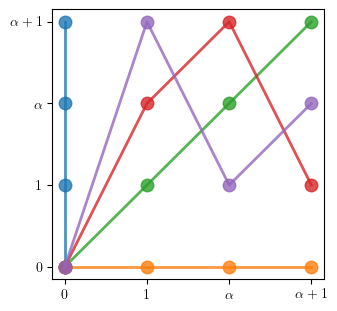
\includegraphics[width=0.5\textwidth]{imgs/affine-desargues-2-2.png}
      \caption{Rayos en el espacio de fase discreto sobre el
        campo $\GF\left( 2^2 \right)$.}
      \label{fig:wootters-affine-2-qubits}
    \end{figure}
    Siguiendo a Wootters, podemos construir a los
    generadores del grupo de Pauli, i.e., a las matrices
    generalizadas de Pauli, a partir de las matrices
    $\sigma_x$ y $\sigma_z$. Pero antes que ésto, notemos
    algunas sutilizas a la hora de trabajar con los
    elementos de la extensión de Galois. Si etiquetamos a la
    base estándar de $\C^{4}$ con los elementos de
    $\GF(2^2)$ en el orden en que aparecen en los ejes de la
    figura (\ref{fig:wootters-affine-2-qubits}), tenemos que
    \[
      \ket 0
      = \begin{pmatrix} 1\\0\\0\\0 \end{pmatrix},
      \quad
      \ket{1}
      = \begin{pmatrix} 0\\1\\0\\0 \end{pmatrix},
      \quad
      \ket{\alpha}
      = \begin{pmatrix} 0\\0\\1\\0 \end{pmatrix},
      \quad
      \ket{\alpha+1}
      = \begin{pmatrix} 0\\0\\0\\1 \end{pmatrix}. 
    \] 
    Distintas bases del campo nos brinda distintas maneras
    de factorizar a la base estándar en productos
    tensoriales de la base estándar de $\C^2$. Para que haya
    un correspondencia adecuada entre la base etiquetada por
    elementos del campo de Galois y los productos
    tensoriales, debemos elegir una base adecuada.  En éste
    caso la base $\{\alpha, 1\}$ nos brinda una factorización
    adecuada. En
    ésta base el elemento $\alpha + 1$ visto como un
    elemento del espacio vectorial sobre el campo $\Z_2$
    tiene componentes $(1,1)$, así que 
    \[
      \ket{\alpha + 1}
      = \ket{1} \otimes \ket{1}
      = \begin{pmatrix} 0\\1 \end{pmatrix} 
      \otimes
      \begin{pmatrix} 0\\1 \end{pmatrix} 
      = \begin{pmatrix} 0\\0\\0\\1 \end{pmatrix},
    \] 
    lo cual coincide con la etiquetación predeterminada.
    Ésto es importante para poder asignar estados físicos a
    las etiquetas del espacio de fase discreto en el caso de
    sistemas compuestos.

    Utilizando las construcciones del capítulo siguiente,
    podemos verificar que el siguiente conjunto es un
    conjunto maximal de bases mutuamente insesgadas del
    espacio de Hilbert $\H = \C^{4}$:
    \begin{align}
      \mathcal T(0,1) &\leftrightarrow \left\{
      \begin{pmatrix} 1\\0\\0\\0 \end{pmatrix},
      \begin{pmatrix} 0\\1\\0\\0 \end{pmatrix},
      \begin{pmatrix} 0\\0\\1\\0 \end{pmatrix},
      \begin{pmatrix} 0\\0\\0\\1 \end{pmatrix}
      \right\}, \\
      \mathcal T(1,0) &\leftrightarrow \left\{
      \frac{1}{2} \begin{pmatrix} 1\\1\\1\\1 \end{pmatrix}, 
      \frac{1}{2} \begin{pmatrix} 1\\1\\-1\\-1 \end{pmatrix}, 
      \frac{1}{2} \begin{pmatrix} 1\\-1\\-1\\1 \end{pmatrix},
      \frac{1}{2} \begin{pmatrix} 1\\-1\\1\\-1 \end{pmatrix} 
      \right\}, \\
      \mathcal T(1,1) &\leftrightarrow \left\{
      \frac{1}{2} \begin{pmatrix} 1\\-1\\-i\\-i \end{pmatrix}, 
      \frac{1}{2} \begin{pmatrix} 1\\-1\\i\\i \end{pmatrix},
      \frac{1}{2} \begin{pmatrix} 1\\1\\i\\-i \end{pmatrix},
      \frac{1}{2} \begin{pmatrix} 1\\1\\-i\\i \end{pmatrix}
      \right\}, \\
      \mathcal T(1,\alpha) &\leftrightarrow \left\{
      \frac{1}{2} \begin{pmatrix} 1\\-i\\-1\\-i \end{pmatrix},
      \frac{1}{2} \begin{pmatrix} 1\\-i\\1\\i \end{pmatrix},
      \frac{1}{2} \begin{pmatrix} 1\\i\\1\\-i \end{pmatrix},
      \frac{1}{2} \begin{pmatrix} 1\\i\\-1\\i \end{pmatrix}
      \right\} \\
      \mathcal T(1,\alpha+1) &\leftrightarrow \left\{
      \frac{1}{2} \begin{pmatrix} 1\\-i\\-i\\-1 \end{pmatrix},
      \frac{1}{2} \begin{pmatrix} 1\\-i\\i\\1 \end{pmatrix},
      \frac{1}{2} \begin{pmatrix} 1\\i\\i\\-1 \end{pmatrix},
      \frac{1}{2} \begin{pmatrix} 1\\i\\-i\\1 \end{pmatrix}
      \right\}.
    \end{align}
    Dadas las bases, utilizamos la misma convención que en
    el ejemplo anterior, asignamos el primer vector de cada
    base al rayo con la pendiente correspondiente. Así por
    ejemplo la primera base corresponde a los eigenvectores
    de los operadores de traslación $D(0,u)$. Con las bases
    asignadas podemos formar los operadores puntuales y
    enseguida la función de Wigner para cualquier estado
    cuántico válido. A manera ilustrativa de nuevo
    calculamos el operador puntual que corresponde al
    origen:
    \[
      A(0,0)
      = \sum_{\lambda \ni (0,0)}^{} Q(\lambda) - I
      = \begin{pmatrix} 
        1 & \frac{i}{2} & \frac{i}{2} & \frac{i}{2} \\[6pt]
        -\frac{i}{2} & 0 & \frac{1}{2} & \frac{1}{2} \\[6pt]
        -\frac{i}{2} & \frac{1}{2} & 0 & \frac{1}{2} \\[6pt]
        -\frac{1}{2} & \frac{1}{2} & \frac{1}{2} & 0
      \end{pmatrix}. 
    \] 
    Vamos graficar la función de Wigner de tres estados
    cuánticos. Si denotamos la base estándar de $\C^2$,
    $\ket 0$ por $\ket \uparrow$ y $\ket 1$ por $\ket
    \downarrow$ entonces podemos etiquetar al eje horizontal
    del espacio de fase como
    \begin{table}[ht]
      \centering
      \begin{tabular}{c|c|c|c}
        0 & 1 & $\alpha$ & $\alpha + 1$ \\[6pt]
        $\ket{00}$ & $\ket{01}$ & $\ket{10}$ & $\ket{11}$
        \\[6pt]
        $\ket{\uparrow \uparrow}$ &
        $\ket{\uparrow\downarrow}$ &
        $\ket{\downarrow\uparrow}$ &
        $\ket{\downarrow\downarrow}$
      \end{tabular}
      \caption{Espacio de fase discreto etiquetado por los
      estados de dos qubits.}
    \end{table}
    De una manera análoga, podemos etiquetar a los elementos
    del eje vertical con otra base ortonormal de $\C^{4}$,
    los que corresponden al conjunto de eigenvectores
    simultáneos de los operadores de desplazamiento
    horizontales. Denotemos a los eigenvectores del
    segundo conjunto de las MUBs por los estados
    $\ket{\rightarrow\rightarrow},
    \ket{\rightarrow\leftarrow},
    \ket{\leftarrow\rightarrow}$ y
    $\ket{\leftarrow\leftarrow}$. Con ésto podemos etiquetar
    al espacio de fase discreto de la siguiente de la manera
    en que aparece en la figura \ref{tab:state_phase_space}.
    
    \begin{table}[!ht]
      \centering
      \begin{tabular}{c c c c c}
        $\ket{\leftarrow\leftarrow}$ & $\circ$ & $\circ$ &
        $\circ$ & $\circ$ \\[7pt]
        $\ket{\leftarrow\rightarrow}$ & $\circ$ & $\circ$ &
        $\circ$ & $\circ$ \\[7pt]
        $\ket{\rightarrow\leftarrow}$ & $\circ$ & $\circ$ &
        $\circ$ & $\circ$ \\[7pt]
        $\ket{\rightarrow\rightarrow}$ & $\circ$ & $\circ$ &
        $\circ$ & $\circ$ \\[7pt]
        & $\ket{\uparrow\uparrow}$ &
        $\ket{\uparrow\downarrow}$
        & $\ket{\downarrow\uparrow}$ &
        $\ket{\downarrow\downarrow}$
      \end{tabular}
      \caption{Etiquetación del espacio de fase discreto
      para $\GF(2^2)$ por eigenestados.}
      \label{tab:state_phase_space}
    \end{table}

    Con tal etiquetación, graficamos la función de Wigner de
    los siguientes estados cuánticos:
    \[
      \ket{\psi_1}
      = \ket{\uparrow\uparrow},
      \quad
      \text{y}
      \quad
      \ket{\psi_2}
      = \frac{1}{\sqrt{2}} \left( \ket{\uparrow\downarrow} -
      \ket{\downarrow\uparrow} \right). 
    \]
    
    \begin{figure}[ht]
      \centering
      %\scalebox{0.7}{
      %  %% Creator: Matplotlib, PGF backend
%%
%% To include the figure in your LaTeX document, write
%%   \input{<filename>.pgf}
%%
%% Make sure the required packages are loaded in your preamble
%%   \usepackage{pgf}
%%
%% Also ensure that all the required font packages are loaded; for instance,
%% the lmodern package is sometimes necessary when using math font.
%%   \usepackage{lmodern}
%%
%% Figures using additional raster images can only be included by \input if
%% they are in the same directory as the main LaTeX file. For loading figures
%% from other directories you can use the `import` package
%%   \usepackage{import}
%%
%% and then include the figures with
%%   \import{<path to file>}{<filename>.pgf}
%%
%% Matplotlib used the following preamble
%%   
%%   \makeatletter\@ifpackageloaded{underscore}{}{\usepackage[strings]{underscore}}\makeatother
%%
\begingroup%
\makeatletter%
\begin{pgfpicture}%
\pgfpathrectangle{\pgfpointorigin}{\pgfqpoint{4.500000in}{3.500000in}}%
\pgfusepath{use as bounding box, clip}%
\begin{pgfscope}%
\pgfsetbuttcap%
\pgfsetmiterjoin%
\definecolor{currentfill}{rgb}{1.000000,1.000000,1.000000}%
\pgfsetfillcolor{currentfill}%
\pgfsetlinewidth{0.000000pt}%
\definecolor{currentstroke}{rgb}{1.000000,1.000000,1.000000}%
\pgfsetstrokecolor{currentstroke}%
\pgfsetdash{}{0pt}%
\pgfpathmoveto{\pgfqpoint{0.000000in}{0.000000in}}%
\pgfpathlineto{\pgfqpoint{4.500000in}{0.000000in}}%
\pgfpathlineto{\pgfqpoint{4.500000in}{3.500000in}}%
\pgfpathlineto{\pgfqpoint{0.000000in}{3.500000in}}%
\pgfpathlineto{\pgfqpoint{0.000000in}{0.000000in}}%
\pgfpathclose%
\pgfusepath{fill}%
\end{pgfscope}%
\begin{pgfscope}%
\pgfsetbuttcap%
\pgfsetmiterjoin%
\definecolor{currentfill}{rgb}{1.000000,1.000000,1.000000}%
\pgfsetfillcolor{currentfill}%
\pgfsetlinewidth{0.000000pt}%
\definecolor{currentstroke}{rgb}{0.000000,0.000000,0.000000}%
\pgfsetstrokecolor{currentstroke}%
\pgfsetstrokeopacity{0.000000}%
\pgfsetdash{}{0pt}%
\pgfpathmoveto{\pgfqpoint{0.562500in}{0.599063in}}%
\pgfpathlineto{\pgfqpoint{2.829375in}{0.599063in}}%
\pgfpathlineto{\pgfqpoint{2.829375in}{2.865938in}}%
\pgfpathlineto{\pgfqpoint{0.562500in}{2.865938in}}%
\pgfpathlineto{\pgfqpoint{0.562500in}{0.599063in}}%
\pgfpathclose%
\pgfusepath{fill}%
\end{pgfscope}%
\begin{pgfscope}%
\pgfsetbuttcap%
\pgfsetmiterjoin%
\definecolor{currentfill}{rgb}{0.950000,0.950000,0.950000}%
\pgfsetfillcolor{currentfill}%
\pgfsetfillopacity{0.500000}%
\pgfsetlinewidth{1.003750pt}%
\definecolor{currentstroke}{rgb}{0.950000,0.950000,0.950000}%
\pgfsetstrokecolor{currentstroke}%
\pgfsetstrokeopacity{0.500000}%
\pgfsetdash{}{0pt}%
\pgfpathmoveto{\pgfqpoint{0.747551in}{1.430281in}}%
\pgfpathlineto{\pgfqpoint{1.890368in}{1.886175in}}%
\pgfpathlineto{\pgfqpoint{1.898416in}{2.752043in}}%
\pgfpathlineto{\pgfqpoint{0.696721in}{2.321580in}}%
\pgfusepath{stroke,fill}%
\end{pgfscope}%
\begin{pgfscope}%
\pgfsetbuttcap%
\pgfsetmiterjoin%
\definecolor{currentfill}{rgb}{0.900000,0.900000,0.900000}%
\pgfsetfillcolor{currentfill}%
\pgfsetfillopacity{0.500000}%
\pgfsetlinewidth{1.003750pt}%
\definecolor{currentstroke}{rgb}{0.900000,0.900000,0.900000}%
\pgfsetstrokecolor{currentstroke}%
\pgfsetstrokeopacity{0.500000}%
\pgfsetdash{}{0pt}%
\pgfpathmoveto{\pgfqpoint{1.890368in}{1.886175in}}%
\pgfpathlineto{\pgfqpoint{2.728721in}{1.219708in}}%
\pgfpathlineto{\pgfqpoint{2.782047in}{2.121980in}}%
\pgfpathlineto{\pgfqpoint{1.898416in}{2.752043in}}%
\pgfusepath{stroke,fill}%
\end{pgfscope}%
\begin{pgfscope}%
\pgfsetbuttcap%
\pgfsetmiterjoin%
\definecolor{currentfill}{rgb}{0.925000,0.925000,0.925000}%
\pgfsetfillcolor{currentfill}%
\pgfsetfillopacity{0.500000}%
\pgfsetlinewidth{1.003750pt}%
\definecolor{currentstroke}{rgb}{0.925000,0.925000,0.925000}%
\pgfsetstrokecolor{currentstroke}%
\pgfsetstrokeopacity{0.500000}%
\pgfsetdash{}{0pt}%
\pgfpathmoveto{\pgfqpoint{0.747551in}{1.430281in}}%
\pgfpathlineto{\pgfqpoint{1.539544in}{0.686862in}}%
\pgfpathlineto{\pgfqpoint{2.728721in}{1.219708in}}%
\pgfpathlineto{\pgfqpoint{1.890368in}{1.886175in}}%
\pgfusepath{stroke,fill}%
\end{pgfscope}%
\begin{pgfscope}%
\pgfsetrectcap%
\pgfsetroundjoin%
\pgfsetlinewidth{0.803000pt}%
\definecolor{currentstroke}{rgb}{0.000000,0.000000,0.000000}%
\pgfsetstrokecolor{currentstroke}%
\pgfsetdash{}{0pt}%
\pgfpathmoveto{\pgfqpoint{0.747551in}{1.430281in}}%
\pgfpathlineto{\pgfqpoint{1.539544in}{0.686862in}}%
\pgfusepath{stroke}%
\end{pgfscope}%
\begin{pgfscope}%
\pgfsetbuttcap%
\pgfsetroundjoin%
\pgfsetlinewidth{0.803000pt}%
\definecolor{currentstroke}{rgb}{0.690196,0.690196,0.690196}%
\pgfsetstrokecolor{currentstroke}%
\pgfsetdash{}{0pt}%
\pgfpathmoveto{\pgfqpoint{0.777375in}{1.402286in}}%
\pgfpathlineto{\pgfqpoint{1.922068in}{1.860975in}}%
\pgfpathlineto{\pgfqpoint{1.931703in}{2.728309in}}%
\pgfusepath{stroke}%
\end{pgfscope}%
\begin{pgfscope}%
\pgfsetbuttcap%
\pgfsetroundjoin%
\pgfsetlinewidth{0.803000pt}%
\definecolor{currentstroke}{rgb}{0.690196,0.690196,0.690196}%
\pgfsetstrokecolor{currentstroke}%
\pgfsetdash{}{0pt}%
\pgfpathmoveto{\pgfqpoint{0.949372in}{1.240839in}}%
\pgfpathlineto{\pgfqpoint{2.104681in}{1.715803in}}%
\pgfpathlineto{\pgfqpoint{2.123652in}{2.591442in}}%
\pgfusepath{stroke}%
\end{pgfscope}%
\begin{pgfscope}%
\pgfsetbuttcap%
\pgfsetroundjoin%
\pgfsetlinewidth{0.803000pt}%
\definecolor{currentstroke}{rgb}{0.690196,0.690196,0.690196}%
\pgfsetstrokecolor{currentstroke}%
\pgfsetdash{}{0pt}%
\pgfpathmoveto{\pgfqpoint{1.127694in}{1.073453in}}%
\pgfpathlineto{\pgfqpoint{2.293654in}{1.565575in}}%
\pgfpathlineto{\pgfqpoint{2.322627in}{2.449565in}}%
\pgfusepath{stroke}%
\end{pgfscope}%
\begin{pgfscope}%
\pgfsetbuttcap%
\pgfsetroundjoin%
\pgfsetlinewidth{0.803000pt}%
\definecolor{currentstroke}{rgb}{0.690196,0.690196,0.690196}%
\pgfsetstrokecolor{currentstroke}%
\pgfsetdash{}{0pt}%
\pgfpathmoveto{\pgfqpoint{1.312698in}{0.899796in}}%
\pgfpathlineto{\pgfqpoint{2.489324in}{1.410022in}}%
\pgfpathlineto{\pgfqpoint{2.529021in}{2.302397in}}%
\pgfusepath{stroke}%
\end{pgfscope}%
\begin{pgfscope}%
\pgfsetbuttcap%
\pgfsetroundjoin%
\pgfsetlinewidth{0.803000pt}%
\definecolor{currentstroke}{rgb}{0.690196,0.690196,0.690196}%
\pgfsetstrokecolor{currentstroke}%
\pgfsetdash{}{0pt}%
\pgfpathmoveto{\pgfqpoint{1.504765in}{0.719508in}}%
\pgfpathlineto{\pgfqpoint{2.692056in}{1.248856in}}%
\pgfpathlineto{\pgfqpoint{2.743258in}{2.149638in}}%
\pgfusepath{stroke}%
\end{pgfscope}%
\begin{pgfscope}%
\pgfsetrectcap%
\pgfsetroundjoin%
\pgfsetlinewidth{0.803000pt}%
\definecolor{currentstroke}{rgb}{0.000000,0.000000,0.000000}%
\pgfsetstrokecolor{currentstroke}%
\pgfsetdash{}{0pt}%
\pgfpathmoveto{\pgfqpoint{0.787024in}{1.406153in}}%
\pgfpathlineto{\pgfqpoint{0.758053in}{1.394544in}}%
\pgfusepath{stroke}%
\end{pgfscope}%
\begin{pgfscope}%
\definecolor{textcolor}{rgb}{0.000000,0.000000,0.000000}%
\pgfsetstrokecolor{textcolor}%
\pgfsetfillcolor{textcolor}%
\pgftext[x=0.620406in,y=1.221969in,,top]{\color{textcolor}\rmfamily\fontsize{10.000000}{12.000000}\selectfont \(\displaystyle \uparrow\uparrow\)}%
\end{pgfscope}%
\begin{pgfscope}%
\pgfsetrectcap%
\pgfsetroundjoin%
\pgfsetlinewidth{0.803000pt}%
\definecolor{currentstroke}{rgb}{0.000000,0.000000,0.000000}%
\pgfsetstrokecolor{currentstroke}%
\pgfsetdash{}{0pt}%
\pgfpathmoveto{\pgfqpoint{0.959119in}{1.244846in}}%
\pgfpathlineto{\pgfqpoint{0.929852in}{1.232814in}}%
\pgfusepath{stroke}%
\end{pgfscope}%
\begin{pgfscope}%
\definecolor{textcolor}{rgb}{0.000000,0.000000,0.000000}%
\pgfsetstrokecolor{textcolor}%
\pgfsetfillcolor{textcolor}%
\pgftext[x=0.789674in,y=1.057162in,,top]{\color{textcolor}\rmfamily\fontsize{10.000000}{12.000000}\selectfont \(\displaystyle \uparrow\downarrow\)}%
\end{pgfscope}%
\begin{pgfscope}%
\pgfsetrectcap%
\pgfsetroundjoin%
\pgfsetlinewidth{0.803000pt}%
\definecolor{currentstroke}{rgb}{0.000000,0.000000,0.000000}%
\pgfsetstrokecolor{currentstroke}%
\pgfsetdash{}{0pt}%
\pgfpathmoveto{\pgfqpoint{1.137540in}{1.077609in}}%
\pgfpathlineto{\pgfqpoint{1.107975in}{1.065130in}}%
\pgfusepath{stroke}%
\end{pgfscope}%
\begin{pgfscope}%
\definecolor{textcolor}{rgb}{0.000000,0.000000,0.000000}%
\pgfsetstrokecolor{textcolor}%
\pgfsetfillcolor{textcolor}%
\pgftext[x=0.965172in,y=0.886290in,,top]{\color{textcolor}\rmfamily\fontsize{10.000000}{12.000000}\selectfont \(\displaystyle \downarrow\uparrow\)}%
\end{pgfscope}%
\begin{pgfscope}%
\pgfsetrectcap%
\pgfsetroundjoin%
\pgfsetlinewidth{0.803000pt}%
\definecolor{currentstroke}{rgb}{0.000000,0.000000,0.000000}%
\pgfsetstrokecolor{currentstroke}%
\pgfsetdash{}{0pt}%
\pgfpathmoveto{\pgfqpoint{1.322644in}{0.904109in}}%
\pgfpathlineto{\pgfqpoint{1.292778in}{0.891158in}}%
\pgfusepath{stroke}%
\end{pgfscope}%
\begin{pgfscope}%
\definecolor{textcolor}{rgb}{0.000000,0.000000,0.000000}%
\pgfsetstrokecolor{textcolor}%
\pgfsetfillcolor{textcolor}%
\pgftext[x=1.147250in,y=0.709010in,,top]{\color{textcolor}\rmfamily\fontsize{10.000000}{12.000000}\selectfont \(\displaystyle \downarrow\downarrow\)}%
\end{pgfscope}%
\begin{pgfscope}%
\pgfsetrectcap%
\pgfsetroundjoin%
\pgfsetlinewidth{0.803000pt}%
\definecolor{currentstroke}{rgb}{0.000000,0.000000,0.000000}%
\pgfsetstrokecolor{currentstroke}%
\pgfsetdash{}{0pt}%
\pgfpathmoveto{\pgfqpoint{1.514812in}{0.723987in}}%
\pgfpathlineto{\pgfqpoint{1.484644in}{0.710537in}}%
\pgfusepath{stroke}%
\end{pgfscope}%
\begin{pgfscope}%
\pgfsetrectcap%
\pgfsetroundjoin%
\pgfsetlinewidth{0.803000pt}%
\definecolor{currentstroke}{rgb}{0.000000,0.000000,0.000000}%
\pgfsetstrokecolor{currentstroke}%
\pgfsetdash{}{0pt}%
\pgfpathmoveto{\pgfqpoint{2.728721in}{1.219708in}}%
\pgfpathlineto{\pgfqpoint{1.539544in}{0.686862in}}%
\pgfusepath{stroke}%
\end{pgfscope}%
\begin{pgfscope}%
\pgfsetbuttcap%
\pgfsetroundjoin%
\pgfsetlinewidth{0.803000pt}%
\definecolor{currentstroke}{rgb}{0.690196,0.690196,0.690196}%
\pgfsetstrokecolor{currentstroke}%
\pgfsetdash{}{0pt}%
\pgfpathmoveto{\pgfqpoint{0.921077in}{2.401947in}}%
\pgfpathlineto{\pgfqpoint{0.960455in}{1.515213in}}%
\pgfpathlineto{\pgfqpoint{1.761853in}{0.786474in}}%
\pgfusepath{stroke}%
\end{pgfscope}%
\begin{pgfscope}%
\pgfsetbuttcap%
\pgfsetroundjoin%
\pgfsetlinewidth{0.803000pt}%
\definecolor{currentstroke}{rgb}{0.690196,0.690196,0.690196}%
\pgfsetstrokecolor{currentstroke}%
\pgfsetdash{}{0pt}%
\pgfpathmoveto{\pgfqpoint{1.203262in}{2.503030in}}%
\pgfpathlineto{\pgfqpoint{1.228535in}{1.622156in}}%
\pgfpathlineto{\pgfqpoint{2.041274in}{0.911677in}}%
\pgfusepath{stroke}%
\end{pgfscope}%
\begin{pgfscope}%
\pgfsetbuttcap%
\pgfsetroundjoin%
\pgfsetlinewidth{0.803000pt}%
\definecolor{currentstroke}{rgb}{0.690196,0.690196,0.690196}%
\pgfsetstrokecolor{currentstroke}%
\pgfsetdash{}{0pt}%
\pgfpathmoveto{\pgfqpoint{1.478354in}{2.601571in}}%
\pgfpathlineto{\pgfqpoint{1.490198in}{1.726539in}}%
\pgfpathlineto{\pgfqpoint{2.313468in}{1.033642in}}%
\pgfusepath{stroke}%
\end{pgfscope}%
\begin{pgfscope}%
\pgfsetbuttcap%
\pgfsetroundjoin%
\pgfsetlinewidth{0.803000pt}%
\definecolor{currentstroke}{rgb}{0.690196,0.690196,0.690196}%
\pgfsetstrokecolor{currentstroke}%
\pgfsetdash{}{0pt}%
\pgfpathmoveto{\pgfqpoint{1.746616in}{2.697666in}}%
\pgfpathlineto{\pgfqpoint{1.745671in}{1.828452in}}%
\pgfpathlineto{\pgfqpoint{2.578712in}{1.152492in}}%
\pgfusepath{stroke}%
\end{pgfscope}%
\begin{pgfscope}%
\pgfsetrectcap%
\pgfsetroundjoin%
\pgfsetlinewidth{0.803000pt}%
\definecolor{currentstroke}{rgb}{0.000000,0.000000,0.000000}%
\pgfsetstrokecolor{currentstroke}%
\pgfsetdash{}{0pt}%
\pgfpathmoveto{\pgfqpoint{1.754918in}{0.792781in}}%
\pgfpathlineto{\pgfqpoint{1.775753in}{0.773835in}}%
\pgfusepath{stroke}%
\end{pgfscope}%
\begin{pgfscope}%
\definecolor{textcolor}{rgb}{0.000000,0.000000,0.000000}%
\pgfsetstrokecolor{textcolor}%
\pgfsetfillcolor{textcolor}%
\pgftext[x=1.879436in,y=0.560550in,,top]{\color{textcolor}\rmfamily\fontsize{10.000000}{12.000000}\selectfont \(\displaystyle \rightarrow\rightarrow\)}%
\end{pgfscope}%
\begin{pgfscope}%
\pgfsetrectcap%
\pgfsetroundjoin%
\pgfsetlinewidth{0.803000pt}%
\definecolor{currentstroke}{rgb}{0.000000,0.000000,0.000000}%
\pgfsetstrokecolor{currentstroke}%
\pgfsetdash{}{0pt}%
\pgfpathmoveto{\pgfqpoint{2.034247in}{0.917820in}}%
\pgfpathlineto{\pgfqpoint{2.055356in}{0.899367in}}%
\pgfusepath{stroke}%
\end{pgfscope}%
\begin{pgfscope}%
\definecolor{textcolor}{rgb}{0.000000,0.000000,0.000000}%
\pgfsetstrokecolor{textcolor}%
\pgfsetfillcolor{textcolor}%
\pgftext[x=2.158420in,y=0.689222in,,top]{\color{textcolor}\rmfamily\fontsize{10.000000}{12.000000}\selectfont \(\displaystyle \rightarrow\leftarrow\)}%
\end{pgfscope}%
\begin{pgfscope}%
\pgfsetrectcap%
\pgfsetroundjoin%
\pgfsetlinewidth{0.803000pt}%
\definecolor{currentstroke}{rgb}{0.000000,0.000000,0.000000}%
\pgfsetstrokecolor{currentstroke}%
\pgfsetdash{}{0pt}%
\pgfpathmoveto{\pgfqpoint{2.306357in}{1.039627in}}%
\pgfpathlineto{\pgfqpoint{2.327718in}{1.021649in}}%
\pgfusepath{stroke}%
\end{pgfscope}%
\begin{pgfscope}%
\definecolor{textcolor}{rgb}{0.000000,0.000000,0.000000}%
\pgfsetstrokecolor{textcolor}%
\pgfsetfillcolor{textcolor}%
\pgftext[x=2.430160in,y=0.814552in,,top]{\color{textcolor}\rmfamily\fontsize{10.000000}{12.000000}\selectfont \(\displaystyle \leftarrow\rightarrow\)}%
\end{pgfscope}%
\begin{pgfscope}%
\pgfsetrectcap%
\pgfsetroundjoin%
\pgfsetlinewidth{0.803000pt}%
\definecolor{currentstroke}{rgb}{0.000000,0.000000,0.000000}%
\pgfsetstrokecolor{currentstroke}%
\pgfsetdash{}{0pt}%
\pgfpathmoveto{\pgfqpoint{2.571523in}{1.158326in}}%
\pgfpathlineto{\pgfqpoint{2.593117in}{1.140803in}}%
\pgfusepath{stroke}%
\end{pgfscope}%
\begin{pgfscope}%
\definecolor{textcolor}{rgb}{0.000000,0.000000,0.000000}%
\pgfsetstrokecolor{textcolor}%
\pgfsetfillcolor{textcolor}%
\pgftext[x=2.694935in,y=0.936671in,,top]{\color{textcolor}\rmfamily\fontsize{10.000000}{12.000000}\selectfont \(\displaystyle \leftarrow\leftarrow\)}%
\end{pgfscope}%
\begin{pgfscope}%
\pgfsetrectcap%
\pgfsetroundjoin%
\pgfsetlinewidth{0.803000pt}%
\definecolor{currentstroke}{rgb}{0.000000,0.000000,0.000000}%
\pgfsetstrokecolor{currentstroke}%
\pgfsetdash{}{0pt}%
\pgfpathmoveto{\pgfqpoint{2.728721in}{1.219708in}}%
\pgfpathlineto{\pgfqpoint{2.782047in}{2.121980in}}%
\pgfusepath{stroke}%
\end{pgfscope}%
\begin{pgfscope}%
\pgfsetbuttcap%
\pgfsetroundjoin%
\pgfsetlinewidth{0.803000pt}%
\definecolor{currentstroke}{rgb}{0.690196,0.690196,0.690196}%
\pgfsetstrokecolor{currentstroke}%
\pgfsetdash{}{0pt}%
\pgfpathmoveto{\pgfqpoint{2.729735in}{1.236859in}}%
\pgfpathlineto{\pgfqpoint{1.890522in}{1.902697in}}%
\pgfpathlineto{\pgfqpoint{0.746584in}{1.447244in}}%
\pgfusepath{stroke}%
\end{pgfscope}%
\begin{pgfscope}%
\pgfsetbuttcap%
\pgfsetroundjoin%
\pgfsetlinewidth{0.803000pt}%
\definecolor{currentstroke}{rgb}{0.690196,0.690196,0.690196}%
\pgfsetstrokecolor{currentstroke}%
\pgfsetdash{}{0pt}%
\pgfpathmoveto{\pgfqpoint{2.739571in}{1.403292in}}%
\pgfpathlineto{\pgfqpoint{1.892011in}{2.062897in}}%
\pgfpathlineto{\pgfqpoint{0.737199in}{1.611809in}}%
\pgfusepath{stroke}%
\end{pgfscope}%
\begin{pgfscope}%
\pgfsetbuttcap%
\pgfsetroundjoin%
\pgfsetlinewidth{0.803000pt}%
\definecolor{currentstroke}{rgb}{0.690196,0.690196,0.690196}%
\pgfsetstrokecolor{currentstroke}%
\pgfsetdash{}{0pt}%
\pgfpathmoveto{\pgfqpoint{2.749602in}{1.573021in}}%
\pgfpathlineto{\pgfqpoint{1.893527in}{2.226034in}}%
\pgfpathlineto{\pgfqpoint{0.727632in}{1.779557in}}%
\pgfusepath{stroke}%
\end{pgfscope}%
\begin{pgfscope}%
\pgfsetbuttcap%
\pgfsetroundjoin%
\pgfsetlinewidth{0.803000pt}%
\definecolor{currentstroke}{rgb}{0.690196,0.690196,0.690196}%
\pgfsetstrokecolor{currentstroke}%
\pgfsetdash{}{0pt}%
\pgfpathmoveto{\pgfqpoint{2.759834in}{1.746145in}}%
\pgfpathlineto{\pgfqpoint{1.895072in}{2.392188in}}%
\pgfpathlineto{\pgfqpoint{0.717879in}{1.950581in}}%
\pgfusepath{stroke}%
\end{pgfscope}%
\begin{pgfscope}%
\pgfsetbuttcap%
\pgfsetroundjoin%
\pgfsetlinewidth{0.803000pt}%
\definecolor{currentstroke}{rgb}{0.690196,0.690196,0.690196}%
\pgfsetstrokecolor{currentstroke}%
\pgfsetdash{}{0pt}%
\pgfpathmoveto{\pgfqpoint{2.770273in}{1.922767in}}%
\pgfpathlineto{\pgfqpoint{1.896645in}{2.561445in}}%
\pgfpathlineto{\pgfqpoint{0.707933in}{2.124978in}}%
\pgfusepath{stroke}%
\end{pgfscope}%
\begin{pgfscope}%
\pgfsetbuttcap%
\pgfsetroundjoin%
\pgfsetlinewidth{0.803000pt}%
\definecolor{currentstroke}{rgb}{0.690196,0.690196,0.690196}%
\pgfsetstrokecolor{currentstroke}%
\pgfsetdash{}{0pt}%
\pgfpathmoveto{\pgfqpoint{2.780925in}{2.102995in}}%
\pgfpathlineto{\pgfqpoint{1.898248in}{2.733893in}}%
\pgfpathlineto{\pgfqpoint{0.697789in}{2.302848in}}%
\pgfusepath{stroke}%
\end{pgfscope}%
\begin{pgfscope}%
\pgfsetrectcap%
\pgfsetroundjoin%
\pgfsetlinewidth{0.803000pt}%
\definecolor{currentstroke}{rgb}{0.000000,0.000000,0.000000}%
\pgfsetstrokecolor{currentstroke}%
\pgfsetdash{}{0pt}%
\pgfpathmoveto{\pgfqpoint{2.722496in}{1.242602in}}%
\pgfpathlineto{\pgfqpoint{2.744239in}{1.225351in}}%
\pgfusepath{stroke}%
\end{pgfscope}%
\begin{pgfscope}%
\definecolor{textcolor}{rgb}{0.000000,0.000000,0.000000}%
\pgfsetstrokecolor{textcolor}%
\pgfsetfillcolor{textcolor}%
\pgftext[x=3.005245in,y=1.207631in,,top]{\color{textcolor}\rmfamily\fontsize{10.000000}{12.000000}\selectfont \(\displaystyle {0.00}\)}%
\end{pgfscope}%
\begin{pgfscope}%
\pgfsetrectcap%
\pgfsetroundjoin%
\pgfsetlinewidth{0.803000pt}%
\definecolor{currentstroke}{rgb}{0.000000,0.000000,0.000000}%
\pgfsetstrokecolor{currentstroke}%
\pgfsetdash{}{0pt}%
\pgfpathmoveto{\pgfqpoint{2.732255in}{1.408985in}}%
\pgfpathlineto{\pgfqpoint{2.754231in}{1.391883in}}%
\pgfusepath{stroke}%
\end{pgfscope}%
\begin{pgfscope}%
\definecolor{textcolor}{rgb}{0.000000,0.000000,0.000000}%
\pgfsetstrokecolor{textcolor}%
\pgfsetfillcolor{textcolor}%
\pgftext[x=3.017824in,y=1.374316in,,top]{\color{textcolor}\rmfamily\fontsize{10.000000}{12.000000}\selectfont \(\displaystyle {0.05}\)}%
\end{pgfscope}%
\begin{pgfscope}%
\pgfsetrectcap%
\pgfsetroundjoin%
\pgfsetlinewidth{0.803000pt}%
\definecolor{currentstroke}{rgb}{0.000000,0.000000,0.000000}%
\pgfsetstrokecolor{currentstroke}%
\pgfsetdash{}{0pt}%
\pgfpathmoveto{\pgfqpoint{2.742208in}{1.578662in}}%
\pgfpathlineto{\pgfqpoint{2.764421in}{1.561718in}}%
\pgfusepath{stroke}%
\end{pgfscope}%
\begin{pgfscope}%
\definecolor{textcolor}{rgb}{0.000000,0.000000,0.000000}%
\pgfsetstrokecolor{textcolor}%
\pgfsetfillcolor{textcolor}%
\pgftext[x=3.030652in,y=1.544313in,,top]{\color{textcolor}\rmfamily\fontsize{10.000000}{12.000000}\selectfont \(\displaystyle {0.10}\)}%
\end{pgfscope}%
\begin{pgfscope}%
\pgfsetrectcap%
\pgfsetroundjoin%
\pgfsetlinewidth{0.803000pt}%
\definecolor{currentstroke}{rgb}{0.000000,0.000000,0.000000}%
\pgfsetstrokecolor{currentstroke}%
\pgfsetdash{}{0pt}%
\pgfpathmoveto{\pgfqpoint{2.752359in}{1.751730in}}%
\pgfpathlineto{\pgfqpoint{2.774814in}{1.734954in}}%
\pgfusepath{stroke}%
\end{pgfscope}%
\begin{pgfscope}%
\definecolor{textcolor}{rgb}{0.000000,0.000000,0.000000}%
\pgfsetstrokecolor{textcolor}%
\pgfsetfillcolor{textcolor}%
\pgftext[x=3.043738in,y=1.717721in,,top]{\color{textcolor}\rmfamily\fontsize{10.000000}{12.000000}\selectfont \(\displaystyle {0.15}\)}%
\end{pgfscope}%
\begin{pgfscope}%
\pgfsetrectcap%
\pgfsetroundjoin%
\pgfsetlinewidth{0.803000pt}%
\definecolor{currentstroke}{rgb}{0.000000,0.000000,0.000000}%
\pgfsetstrokecolor{currentstroke}%
\pgfsetdash{}{0pt}%
\pgfpathmoveto{\pgfqpoint{2.762716in}{1.928292in}}%
\pgfpathlineto{\pgfqpoint{2.785418in}{1.911695in}}%
\pgfusepath{stroke}%
\end{pgfscope}%
\begin{pgfscope}%
\definecolor{textcolor}{rgb}{0.000000,0.000000,0.000000}%
\pgfsetstrokecolor{textcolor}%
\pgfsetfillcolor{textcolor}%
\pgftext[x=3.057090in,y=1.894645in,,top]{\color{textcolor}\rmfamily\fontsize{10.000000}{12.000000}\selectfont \(\displaystyle {0.20}\)}%
\end{pgfscope}%
\begin{pgfscope}%
\pgfsetrectcap%
\pgfsetroundjoin%
\pgfsetlinewidth{0.803000pt}%
\definecolor{currentstroke}{rgb}{0.000000,0.000000,0.000000}%
\pgfsetstrokecolor{currentstroke}%
\pgfsetdash{}{0pt}%
\pgfpathmoveto{\pgfqpoint{2.773283in}{2.108457in}}%
\pgfpathlineto{\pgfqpoint{2.796239in}{2.092049in}}%
\pgfusepath{stroke}%
\end{pgfscope}%
\begin{pgfscope}%
\definecolor{textcolor}{rgb}{0.000000,0.000000,0.000000}%
\pgfsetstrokecolor{textcolor}%
\pgfsetfillcolor{textcolor}%
\pgftext[x=3.070715in,y=2.075193in,,top]{\color{textcolor}\rmfamily\fontsize{10.000000}{12.000000}\selectfont \(\displaystyle {0.25}\)}%
\end{pgfscope}%
\begin{pgfscope}%
\pgfpathrectangle{\pgfqpoint{0.562500in}{0.599063in}}{\pgfqpoint{2.266875in}{2.266875in}}%
\pgfusepath{clip}%
\pgfsetbuttcap%
\pgfsetroundjoin%
\definecolor{currentfill}{rgb}{0.529732,0.483284,0.076766}%
\pgfsetfillcolor{currentfill}%
\pgfsetlinewidth{0.000000pt}%
\definecolor{currentstroke}{rgb}{0.000000,0.000000,0.000000}%
\pgfsetstrokecolor{currentstroke}%
\pgfsetdash{}{0pt}%
\pgfpathmoveto{\pgfqpoint{1.667676in}{1.753951in}}%
\pgfpathlineto{\pgfqpoint{1.870797in}{1.835392in}}%
\pgfpathlineto{\pgfqpoint{2.016559in}{1.718604in}}%
\pgfpathlineto{\pgfqpoint{1.812038in}{1.634901in}}%
\pgfpathlineto{\pgfqpoint{1.667676in}{1.753951in}}%
\pgfpathclose%
\pgfusepath{fill}%
\end{pgfscope}%
\begin{pgfscope}%
\pgfpathrectangle{\pgfqpoint{0.562500in}{0.599063in}}{\pgfqpoint{2.266875in}{2.266875in}}%
\pgfusepath{clip}%
\pgfsetbuttcap%
\pgfsetroundjoin%
\definecolor{currentfill}{rgb}{0.173553,0.003168,0.214120}%
\pgfsetfillcolor{currentfill}%
\pgfsetlinewidth{0.000000pt}%
\definecolor{currentstroke}{rgb}{0.000000,0.000000,0.000000}%
\pgfsetstrokecolor{currentstroke}%
\pgfsetdash{}{0pt}%
\pgfpathmoveto{\pgfqpoint{1.848756in}{1.604621in}}%
\pgfpathlineto{\pgfqpoint{1.848756in}{1.604621in}}%
\pgfpathlineto{\pgfqpoint{2.053627in}{1.688904in}}%
\pgfpathlineto{\pgfqpoint{2.053627in}{1.688904in}}%
\pgfpathlineto{\pgfqpoint{1.848756in}{1.604621in}}%
\pgfpathclose%
\pgfusepath{fill}%
\end{pgfscope}%
\begin{pgfscope}%
\pgfpathrectangle{\pgfqpoint{0.562500in}{0.599063in}}{\pgfqpoint{2.266875in}{2.266875in}}%
\pgfusepath{clip}%
\pgfsetbuttcap%
\pgfsetroundjoin%
\definecolor{currentfill}{rgb}{0.529732,0.483284,0.076766}%
\pgfsetfillcolor{currentfill}%
\pgfsetlinewidth{0.000000pt}%
\definecolor{currentstroke}{rgb}{0.000000,0.000000,0.000000}%
\pgfsetstrokecolor{currentstroke}%
\pgfsetdash{}{0pt}%
\pgfpathmoveto{\pgfqpoint{1.408241in}{1.649932in}}%
\pgfpathlineto{\pgfqpoint{1.616287in}{1.733347in}}%
\pgfpathlineto{\pgfqpoint{1.760286in}{1.613721in}}%
\pgfpathlineto{\pgfqpoint{1.550735in}{1.527960in}}%
\pgfpathlineto{\pgfqpoint{1.408241in}{1.649932in}}%
\pgfpathclose%
\pgfusepath{fill}%
\end{pgfscope}%
\begin{pgfscope}%
\pgfpathrectangle{\pgfqpoint{0.562500in}{0.599063in}}{\pgfqpoint{2.266875in}{2.266875in}}%
\pgfusepath{clip}%
\pgfsetbuttcap%
\pgfsetroundjoin%
\definecolor{currentfill}{rgb}{0.173553,0.003168,0.214120}%
\pgfsetfillcolor{currentfill}%
\pgfsetlinewidth{0.000000pt}%
\definecolor{currentstroke}{rgb}{0.000000,0.000000,0.000000}%
\pgfsetstrokecolor{currentstroke}%
\pgfsetdash{}{0pt}%
\pgfpathmoveto{\pgfqpoint{2.053627in}{1.688904in}}%
\pgfpathlineto{\pgfqpoint{2.053627in}{1.688904in}}%
\pgfpathlineto{\pgfqpoint{2.204488in}{1.568032in}}%
\pgfpathlineto{\pgfqpoint{2.204488in}{1.568032in}}%
\pgfpathlineto{\pgfqpoint{2.053627in}{1.688904in}}%
\pgfpathclose%
\pgfusepath{fill}%
\end{pgfscope}%
\begin{pgfscope}%
\pgfpathrectangle{\pgfqpoint{0.562500in}{0.599063in}}{\pgfqpoint{2.266875in}{2.266875in}}%
\pgfusepath{clip}%
\pgfsetbuttcap%
\pgfsetroundjoin%
\definecolor{currentfill}{rgb}{0.877369,0.800439,0.127143}%
\pgfsetfillcolor{currentfill}%
\pgfsetlinewidth{0.000000pt}%
\definecolor{currentstroke}{rgb}{0.000000,0.000000,0.000000}%
\pgfsetstrokecolor{currentstroke}%
\pgfsetdash{}{0pt}%
\pgfpathmoveto{\pgfqpoint{1.667676in}{1.753951in}}%
\pgfpathlineto{\pgfqpoint{1.664850in}{2.593360in}}%
\pgfpathlineto{\pgfqpoint{1.877650in}{2.670333in}}%
\pgfpathlineto{\pgfqpoint{1.870797in}{1.835392in}}%
\pgfpathlineto{\pgfqpoint{1.667676in}{1.753951in}}%
\pgfpathclose%
\pgfusepath{fill}%
\end{pgfscope}%
\begin{pgfscope}%
\pgfpathrectangle{\pgfqpoint{0.562500in}{0.599063in}}{\pgfqpoint{2.266875in}{2.266875in}}%
\pgfusepath{clip}%
\pgfsetbuttcap%
\pgfsetroundjoin%
\definecolor{currentfill}{rgb}{0.204703,0.003737,0.252551}%
\pgfsetfillcolor{currentfill}%
\pgfsetlinewidth{0.000000pt}%
\definecolor{currentstroke}{rgb}{0.000000,0.000000,0.000000}%
\pgfsetstrokecolor{currentstroke}%
\pgfsetdash{}{0pt}%
\pgfpathmoveto{\pgfqpoint{1.848756in}{1.604621in}}%
\pgfpathlineto{\pgfqpoint{1.998217in}{1.481366in}}%
\pgfpathlineto{\pgfqpoint{2.204488in}{1.568032in}}%
\pgfpathlineto{\pgfqpoint{2.053627in}{1.688904in}}%
\pgfpathlineto{\pgfqpoint{1.848756in}{1.604621in}}%
\pgfpathclose%
\pgfusepath{fill}%
\end{pgfscope}%
\begin{pgfscope}%
\pgfpathrectangle{\pgfqpoint{0.562500in}{0.599063in}}{\pgfqpoint{2.266875in}{2.266875in}}%
\pgfusepath{clip}%
\pgfsetbuttcap%
\pgfsetroundjoin%
\definecolor{currentfill}{rgb}{0.142402,0.002599,0.175688}%
\pgfsetfillcolor{currentfill}%
\pgfsetlinewidth{0.000000pt}%
\definecolor{currentstroke}{rgb}{0.000000,0.000000,0.000000}%
\pgfsetstrokecolor{currentstroke}%
\pgfsetdash{}{0pt}%
\pgfpathmoveto{\pgfqpoint{1.848756in}{1.604621in}}%
\pgfpathlineto{\pgfqpoint{2.053627in}{1.688904in}}%
\pgfpathlineto{\pgfqpoint{2.204488in}{1.568032in}}%
\pgfpathlineto{\pgfqpoint{1.998217in}{1.481366in}}%
\pgfpathlineto{\pgfqpoint{1.848756in}{1.604621in}}%
\pgfpathclose%
\pgfusepath{fill}%
\end{pgfscope}%
\begin{pgfscope}%
\pgfpathrectangle{\pgfqpoint{0.562500in}{0.599063in}}{\pgfqpoint{2.266875in}{2.266875in}}%
\pgfusepath{clip}%
\pgfsetbuttcap%
\pgfsetroundjoin%
\definecolor{currentfill}{rgb}{0.413853,0.377565,0.059973}%
\pgfsetfillcolor{currentfill}%
\pgfsetlinewidth{0.000000pt}%
\definecolor{currentstroke}{rgb}{0.000000,0.000000,0.000000}%
\pgfsetstrokecolor{currentstroke}%
\pgfsetdash{}{0pt}%
\pgfpathmoveto{\pgfqpoint{1.870797in}{1.835392in}}%
\pgfpathlineto{\pgfqpoint{1.877650in}{2.670333in}}%
\pgfpathlineto{\pgfqpoint{2.030536in}{2.559930in}}%
\pgfpathlineto{\pgfqpoint{2.016559in}{1.718604in}}%
\pgfpathlineto{\pgfqpoint{1.870797in}{1.835392in}}%
\pgfpathclose%
\pgfusepath{fill}%
\end{pgfscope}%
\begin{pgfscope}%
\pgfpathrectangle{\pgfqpoint{0.562500in}{0.599063in}}{\pgfqpoint{2.266875in}{2.266875in}}%
\pgfusepath{clip}%
\pgfsetbuttcap%
\pgfsetroundjoin%
\definecolor{currentfill}{rgb}{0.173553,0.003168,0.214120}%
\pgfsetfillcolor{currentfill}%
\pgfsetlinewidth{0.000000pt}%
\definecolor{currentstroke}{rgb}{0.000000,0.000000,0.000000}%
\pgfsetstrokecolor{currentstroke}%
\pgfsetdash{}{0pt}%
\pgfpathmoveto{\pgfqpoint{1.848756in}{1.604621in}}%
\pgfpathlineto{\pgfqpoint{1.998217in}{1.481366in}}%
\pgfpathlineto{\pgfqpoint{1.998217in}{1.481366in}}%
\pgfpathlineto{\pgfqpoint{1.848756in}{1.604621in}}%
\pgfpathlineto{\pgfqpoint{1.848756in}{1.604621in}}%
\pgfpathclose%
\pgfusepath{fill}%
\end{pgfscope}%
\begin{pgfscope}%
\pgfpathrectangle{\pgfqpoint{0.562500in}{0.599063in}}{\pgfqpoint{2.266875in}{2.266875in}}%
\pgfusepath{clip}%
\pgfsetbuttcap%
\pgfsetroundjoin%
\definecolor{currentfill}{rgb}{0.173553,0.003168,0.214120}%
\pgfsetfillcolor{currentfill}%
\pgfsetlinewidth{0.000000pt}%
\definecolor{currentstroke}{rgb}{0.000000,0.000000,0.000000}%
\pgfsetstrokecolor{currentstroke}%
\pgfsetdash{}{0pt}%
\pgfpathmoveto{\pgfqpoint{1.586986in}{1.496930in}}%
\pgfpathlineto{\pgfqpoint{1.586986in}{1.496930in}}%
\pgfpathlineto{\pgfqpoint{1.796913in}{1.583293in}}%
\pgfpathlineto{\pgfqpoint{1.796913in}{1.583293in}}%
\pgfpathlineto{\pgfqpoint{1.586986in}{1.496930in}}%
\pgfpathclose%
\pgfusepath{fill}%
\end{pgfscope}%
\begin{pgfscope}%
\pgfpathrectangle{\pgfqpoint{0.562500in}{0.599063in}}{\pgfqpoint{2.266875in}{2.266875in}}%
\pgfusepath{clip}%
\pgfsetbuttcap%
\pgfsetroundjoin%
\definecolor{currentfill}{rgb}{0.173553,0.003168,0.214120}%
\pgfsetfillcolor{currentfill}%
\pgfsetlinewidth{0.000000pt}%
\definecolor{currentstroke}{rgb}{0.000000,0.000000,0.000000}%
\pgfsetstrokecolor{currentstroke}%
\pgfsetdash{}{0pt}%
\pgfpathmoveto{\pgfqpoint{1.998217in}{1.481366in}}%
\pgfpathlineto{\pgfqpoint{2.204488in}{1.568032in}}%
\pgfpathlineto{\pgfqpoint{2.204488in}{1.568032in}}%
\pgfpathlineto{\pgfqpoint{1.998217in}{1.481366in}}%
\pgfpathlineto{\pgfqpoint{1.998217in}{1.481366in}}%
\pgfpathclose%
\pgfusepath{fill}%
\end{pgfscope}%
\begin{pgfscope}%
\pgfpathrectangle{\pgfqpoint{0.562500in}{0.599063in}}{\pgfqpoint{2.266875in}{2.266875in}}%
\pgfusepath{clip}%
\pgfsetbuttcap%
\pgfsetroundjoin%
\definecolor{currentfill}{rgb}{0.529732,0.483284,0.076766}%
\pgfsetfillcolor{currentfill}%
\pgfsetlinewidth{0.000000pt}%
\definecolor{currentstroke}{rgb}{0.000000,0.000000,0.000000}%
\pgfsetstrokecolor{currentstroke}%
\pgfsetdash{}{0pt}%
\pgfpathmoveto{\pgfqpoint{1.142444in}{1.543361in}}%
\pgfpathlineto{\pgfqpoint{1.355598in}{1.628824in}}%
\pgfpathlineto{\pgfqpoint{1.497702in}{1.506256in}}%
\pgfpathlineto{\pgfqpoint{1.282935in}{1.418359in}}%
\pgfpathlineto{\pgfqpoint{1.142444in}{1.543361in}}%
\pgfpathclose%
\pgfusepath{fill}%
\end{pgfscope}%
\begin{pgfscope}%
\pgfpathrectangle{\pgfqpoint{0.562500in}{0.599063in}}{\pgfqpoint{2.266875in}{2.266875in}}%
\pgfusepath{clip}%
\pgfsetbuttcap%
\pgfsetroundjoin%
\definecolor{currentfill}{rgb}{0.173553,0.003168,0.214120}%
\pgfsetfillcolor{currentfill}%
\pgfsetlinewidth{0.000000pt}%
\definecolor{currentstroke}{rgb}{0.000000,0.000000,0.000000}%
\pgfsetstrokecolor{currentstroke}%
\pgfsetdash{}{0pt}%
\pgfpathmoveto{\pgfqpoint{1.796913in}{1.583293in}}%
\pgfpathlineto{\pgfqpoint{1.796913in}{1.583293in}}%
\pgfpathlineto{\pgfqpoint{1.946011in}{1.459431in}}%
\pgfpathlineto{\pgfqpoint{1.946011in}{1.459431in}}%
\pgfpathlineto{\pgfqpoint{1.796913in}{1.583293in}}%
\pgfpathclose%
\pgfusepath{fill}%
\end{pgfscope}%
\begin{pgfscope}%
\pgfpathrectangle{\pgfqpoint{0.562500in}{0.599063in}}{\pgfqpoint{2.266875in}{2.266875in}}%
\pgfusepath{clip}%
\pgfsetbuttcap%
\pgfsetroundjoin%
\definecolor{currentfill}{rgb}{0.173553,0.003168,0.214120}%
\pgfsetfillcolor{currentfill}%
\pgfsetlinewidth{0.000000pt}%
\definecolor{currentstroke}{rgb}{0.000000,0.000000,0.000000}%
\pgfsetstrokecolor{currentstroke}%
\pgfsetdash{}{0pt}%
\pgfpathmoveto{\pgfqpoint{2.036243in}{1.450007in}}%
\pgfpathlineto{\pgfqpoint{2.036243in}{1.450007in}}%
\pgfpathlineto{\pgfqpoint{2.242864in}{1.537284in}}%
\pgfpathlineto{\pgfqpoint{2.242864in}{1.537284in}}%
\pgfpathlineto{\pgfqpoint{2.036243in}{1.450007in}}%
\pgfpathclose%
\pgfusepath{fill}%
\end{pgfscope}%
\begin{pgfscope}%
\pgfpathrectangle{\pgfqpoint{0.562500in}{0.599063in}}{\pgfqpoint{2.266875in}{2.266875in}}%
\pgfusepath{clip}%
\pgfsetbuttcap%
\pgfsetroundjoin%
\definecolor{currentfill}{rgb}{0.877369,0.800439,0.127143}%
\pgfsetfillcolor{currentfill}%
\pgfsetlinewidth{0.000000pt}%
\definecolor{currentstroke}{rgb}{0.000000,0.000000,0.000000}%
\pgfsetstrokecolor{currentstroke}%
\pgfsetdash{}{0pt}%
\pgfpathmoveto{\pgfqpoint{1.667676in}{1.753951in}}%
\pgfpathlineto{\pgfqpoint{1.812038in}{1.634901in}}%
\pgfpathlineto{\pgfqpoint{1.816199in}{2.480714in}}%
\pgfpathlineto{\pgfqpoint{1.664850in}{2.593360in}}%
\pgfpathlineto{\pgfqpoint{1.667676in}{1.753951in}}%
\pgfpathclose%
\pgfusepath{fill}%
\end{pgfscope}%
\begin{pgfscope}%
\pgfpathrectangle{\pgfqpoint{0.562500in}{0.599063in}}{\pgfqpoint{2.266875in}{2.266875in}}%
\pgfusepath{clip}%
\pgfsetbuttcap%
\pgfsetroundjoin%
\definecolor{currentfill}{rgb}{0.877369,0.800439,0.127143}%
\pgfsetfillcolor{currentfill}%
\pgfsetlinewidth{0.000000pt}%
\definecolor{currentstroke}{rgb}{0.000000,0.000000,0.000000}%
\pgfsetstrokecolor{currentstroke}%
\pgfsetdash{}{0pt}%
\pgfpathmoveto{\pgfqpoint{1.408241in}{1.649932in}}%
\pgfpathlineto{\pgfqpoint{1.392769in}{2.494944in}}%
\pgfpathlineto{\pgfqpoint{1.610981in}{2.573875in}}%
\pgfpathlineto{\pgfqpoint{1.616287in}{1.733347in}}%
\pgfpathlineto{\pgfqpoint{1.408241in}{1.649932in}}%
\pgfpathclose%
\pgfusepath{fill}%
\end{pgfscope}%
\begin{pgfscope}%
\pgfpathrectangle{\pgfqpoint{0.562500in}{0.599063in}}{\pgfqpoint{2.266875in}{2.266875in}}%
\pgfusepath{clip}%
\pgfsetbuttcap%
\pgfsetroundjoin%
\definecolor{currentfill}{rgb}{0.142402,0.002599,0.175688}%
\pgfsetfillcolor{currentfill}%
\pgfsetlinewidth{0.000000pt}%
\definecolor{currentstroke}{rgb}{0.000000,0.000000,0.000000}%
\pgfsetstrokecolor{currentstroke}%
\pgfsetdash{}{0pt}%
\pgfpathmoveto{\pgfqpoint{1.586986in}{1.496930in}}%
\pgfpathlineto{\pgfqpoint{1.796913in}{1.583293in}}%
\pgfpathlineto{\pgfqpoint{1.946011in}{1.459431in}}%
\pgfpathlineto{\pgfqpoint{1.734576in}{1.370596in}}%
\pgfpathlineto{\pgfqpoint{1.586986in}{1.496930in}}%
\pgfpathclose%
\pgfusepath{fill}%
\end{pgfscope}%
\begin{pgfscope}%
\pgfpathrectangle{\pgfqpoint{0.562500in}{0.599063in}}{\pgfqpoint{2.266875in}{2.266875in}}%
\pgfusepath{clip}%
\pgfsetbuttcap%
\pgfsetroundjoin%
\definecolor{currentfill}{rgb}{0.204703,0.003737,0.252551}%
\pgfsetfillcolor{currentfill}%
\pgfsetlinewidth{0.000000pt}%
\definecolor{currentstroke}{rgb}{0.000000,0.000000,0.000000}%
\pgfsetstrokecolor{currentstroke}%
\pgfsetdash{}{0pt}%
\pgfpathmoveto{\pgfqpoint{1.586986in}{1.496930in}}%
\pgfpathlineto{\pgfqpoint{1.734576in}{1.370596in}}%
\pgfpathlineto{\pgfqpoint{1.946011in}{1.459431in}}%
\pgfpathlineto{\pgfqpoint{1.796913in}{1.583293in}}%
\pgfpathlineto{\pgfqpoint{1.586986in}{1.496930in}}%
\pgfpathclose%
\pgfusepath{fill}%
\end{pgfscope}%
\begin{pgfscope}%
\pgfpathrectangle{\pgfqpoint{0.562500in}{0.599063in}}{\pgfqpoint{2.266875in}{2.266875in}}%
\pgfusepath{clip}%
\pgfsetbuttcap%
\pgfsetroundjoin%
\definecolor{currentfill}{rgb}{0.173553,0.003168,0.214120}%
\pgfsetfillcolor{currentfill}%
\pgfsetlinewidth{0.000000pt}%
\definecolor{currentstroke}{rgb}{0.000000,0.000000,0.000000}%
\pgfsetstrokecolor{currentstroke}%
\pgfsetdash{}{0pt}%
\pgfpathmoveto{\pgfqpoint{2.242864in}{1.537284in}}%
\pgfpathlineto{\pgfqpoint{2.242864in}{1.537284in}}%
\pgfpathlineto{\pgfqpoint{2.399095in}{1.412108in}}%
\pgfpathlineto{\pgfqpoint{2.399095in}{1.412108in}}%
\pgfpathlineto{\pgfqpoint{2.242864in}{1.537284in}}%
\pgfpathclose%
\pgfusepath{fill}%
\end{pgfscope}%
\begin{pgfscope}%
\pgfpathrectangle{\pgfqpoint{0.562500in}{0.599063in}}{\pgfqpoint{2.266875in}{2.266875in}}%
\pgfusepath{clip}%
\pgfsetbuttcap%
\pgfsetroundjoin%
\definecolor{currentfill}{rgb}{0.413853,0.377565,0.059973}%
\pgfsetfillcolor{currentfill}%
\pgfsetlinewidth{0.000000pt}%
\definecolor{currentstroke}{rgb}{0.000000,0.000000,0.000000}%
\pgfsetstrokecolor{currentstroke}%
\pgfsetdash{}{0pt}%
\pgfpathmoveto{\pgfqpoint{1.812038in}{1.634901in}}%
\pgfpathlineto{\pgfqpoint{2.016559in}{1.718604in}}%
\pgfpathlineto{\pgfqpoint{2.030536in}{2.559930in}}%
\pgfpathlineto{\pgfqpoint{1.816199in}{2.480714in}}%
\pgfpathlineto{\pgfqpoint{1.812038in}{1.634901in}}%
\pgfpathclose%
\pgfusepath{fill}%
\end{pgfscope}%
\begin{pgfscope}%
\pgfpathrectangle{\pgfqpoint{0.562500in}{0.599063in}}{\pgfqpoint{2.266875in}{2.266875in}}%
\pgfusepath{clip}%
\pgfsetbuttcap%
\pgfsetroundjoin%
\definecolor{currentfill}{rgb}{0.413853,0.377565,0.059973}%
\pgfsetfillcolor{currentfill}%
\pgfsetlinewidth{0.000000pt}%
\definecolor{currentstroke}{rgb}{0.000000,0.000000,0.000000}%
\pgfsetstrokecolor{currentstroke}%
\pgfsetdash{}{0pt}%
\pgfpathmoveto{\pgfqpoint{1.616287in}{1.733347in}}%
\pgfpathlineto{\pgfqpoint{1.610981in}{2.573875in}}%
\pgfpathlineto{\pgfqpoint{1.761931in}{2.460658in}}%
\pgfpathlineto{\pgfqpoint{1.760286in}{1.613721in}}%
\pgfpathlineto{\pgfqpoint{1.616287in}{1.733347in}}%
\pgfpathclose%
\pgfusepath{fill}%
\end{pgfscope}%
\begin{pgfscope}%
\pgfpathrectangle{\pgfqpoint{0.562500in}{0.599063in}}{\pgfqpoint{2.266875in}{2.266875in}}%
\pgfusepath{clip}%
\pgfsetbuttcap%
\pgfsetroundjoin%
\definecolor{currentfill}{rgb}{0.173553,0.003168,0.214120}%
\pgfsetfillcolor{currentfill}%
\pgfsetlinewidth{0.000000pt}%
\definecolor{currentstroke}{rgb}{0.000000,0.000000,0.000000}%
\pgfsetstrokecolor{currentstroke}%
\pgfsetdash{}{0pt}%
\pgfpathmoveto{\pgfqpoint{1.586986in}{1.496930in}}%
\pgfpathlineto{\pgfqpoint{1.734576in}{1.370596in}}%
\pgfpathlineto{\pgfqpoint{1.734576in}{1.370596in}}%
\pgfpathlineto{\pgfqpoint{1.586986in}{1.496930in}}%
\pgfpathlineto{\pgfqpoint{1.586986in}{1.496930in}}%
\pgfpathclose%
\pgfusepath{fill}%
\end{pgfscope}%
\begin{pgfscope}%
\pgfpathrectangle{\pgfqpoint{0.562500in}{0.599063in}}{\pgfqpoint{2.266875in}{2.266875in}}%
\pgfusepath{clip}%
\pgfsetbuttcap%
\pgfsetroundjoin%
\definecolor{currentfill}{rgb}{0.173553,0.003168,0.214120}%
\pgfsetfillcolor{currentfill}%
\pgfsetlinewidth{0.000000pt}%
\definecolor{currentstroke}{rgb}{0.000000,0.000000,0.000000}%
\pgfsetstrokecolor{currentstroke}%
\pgfsetdash{}{0pt}%
\pgfpathmoveto{\pgfqpoint{1.318683in}{1.386552in}}%
\pgfpathlineto{\pgfqpoint{1.318683in}{1.386552in}}%
\pgfpathlineto{\pgfqpoint{1.533855in}{1.475073in}}%
\pgfpathlineto{\pgfqpoint{1.533855in}{1.475073in}}%
\pgfpathlineto{\pgfqpoint{1.318683in}{1.386552in}}%
\pgfpathclose%
\pgfusepath{fill}%
\end{pgfscope}%
\begin{pgfscope}%
\pgfpathrectangle{\pgfqpoint{0.562500in}{0.599063in}}{\pgfqpoint{2.266875in}{2.266875in}}%
\pgfusepath{clip}%
\pgfsetbuttcap%
\pgfsetroundjoin%
\definecolor{currentfill}{rgb}{0.142402,0.002599,0.175688}%
\pgfsetfillcolor{currentfill}%
\pgfsetlinewidth{0.000000pt}%
\definecolor{currentstroke}{rgb}{0.000000,0.000000,0.000000}%
\pgfsetstrokecolor{currentstroke}%
\pgfsetdash{}{0pt}%
\pgfpathmoveto{\pgfqpoint{2.036243in}{1.450007in}}%
\pgfpathlineto{\pgfqpoint{2.242864in}{1.537284in}}%
\pgfpathlineto{\pgfqpoint{2.399095in}{1.412108in}}%
\pgfpathlineto{\pgfqpoint{2.191078in}{1.322319in}}%
\pgfpathlineto{\pgfqpoint{2.036243in}{1.450007in}}%
\pgfpathclose%
\pgfusepath{fill}%
\end{pgfscope}%
\begin{pgfscope}%
\pgfpathrectangle{\pgfqpoint{0.562500in}{0.599063in}}{\pgfqpoint{2.266875in}{2.266875in}}%
\pgfusepath{clip}%
\pgfsetbuttcap%
\pgfsetroundjoin%
\definecolor{currentfill}{rgb}{0.204703,0.003737,0.252551}%
\pgfsetfillcolor{currentfill}%
\pgfsetlinewidth{0.000000pt}%
\definecolor{currentstroke}{rgb}{0.000000,0.000000,0.000000}%
\pgfsetstrokecolor{currentstroke}%
\pgfsetdash{}{0pt}%
\pgfpathmoveto{\pgfqpoint{2.036243in}{1.450007in}}%
\pgfpathlineto{\pgfqpoint{2.191078in}{1.322319in}}%
\pgfpathlineto{\pgfqpoint{2.399095in}{1.412108in}}%
\pgfpathlineto{\pgfqpoint{2.242864in}{1.537284in}}%
\pgfpathlineto{\pgfqpoint{2.036243in}{1.450007in}}%
\pgfpathclose%
\pgfusepath{fill}%
\end{pgfscope}%
\begin{pgfscope}%
\pgfpathrectangle{\pgfqpoint{0.562500in}{0.599063in}}{\pgfqpoint{2.266875in}{2.266875in}}%
\pgfusepath{clip}%
\pgfsetbuttcap%
\pgfsetroundjoin%
\definecolor{currentfill}{rgb}{0.173553,0.003168,0.214120}%
\pgfsetfillcolor{currentfill}%
\pgfsetlinewidth{0.000000pt}%
\definecolor{currentstroke}{rgb}{0.000000,0.000000,0.000000}%
\pgfsetstrokecolor{currentstroke}%
\pgfsetdash{}{0pt}%
\pgfpathmoveto{\pgfqpoint{1.734576in}{1.370596in}}%
\pgfpathlineto{\pgfqpoint{1.946011in}{1.459431in}}%
\pgfpathlineto{\pgfqpoint{1.946011in}{1.459431in}}%
\pgfpathlineto{\pgfqpoint{1.734576in}{1.370596in}}%
\pgfpathlineto{\pgfqpoint{1.734576in}{1.370596in}}%
\pgfpathclose%
\pgfusepath{fill}%
\end{pgfscope}%
\begin{pgfscope}%
\pgfpathrectangle{\pgfqpoint{0.562500in}{0.599063in}}{\pgfqpoint{2.266875in}{2.266875in}}%
\pgfusepath{clip}%
\pgfsetbuttcap%
\pgfsetroundjoin%
\definecolor{currentfill}{rgb}{0.529732,0.483284,0.076766}%
\pgfsetfillcolor{currentfill}%
\pgfsetlinewidth{0.000000pt}%
\definecolor{currentstroke}{rgb}{0.000000,0.000000,0.000000}%
\pgfsetstrokecolor{currentstroke}%
\pgfsetdash{}{0pt}%
\pgfpathmoveto{\pgfqpoint{0.870050in}{1.434146in}}%
\pgfpathlineto{\pgfqpoint{1.088501in}{1.521733in}}%
\pgfpathlineto{\pgfqpoint{1.228574in}{1.396111in}}%
\pgfpathlineto{\pgfqpoint{1.008391in}{1.305999in}}%
\pgfpathlineto{\pgfqpoint{0.870050in}{1.434146in}}%
\pgfpathclose%
\pgfusepath{fill}%
\end{pgfscope}%
\begin{pgfscope}%
\pgfpathrectangle{\pgfqpoint{0.562500in}{0.599063in}}{\pgfqpoint{2.266875in}{2.266875in}}%
\pgfusepath{clip}%
\pgfsetbuttcap%
\pgfsetroundjoin%
\definecolor{currentfill}{rgb}{0.173553,0.003168,0.214120}%
\pgfsetfillcolor{currentfill}%
\pgfsetlinewidth{0.000000pt}%
\definecolor{currentstroke}{rgb}{0.000000,0.000000,0.000000}%
\pgfsetstrokecolor{currentstroke}%
\pgfsetdash{}{0pt}%
\pgfpathmoveto{\pgfqpoint{1.533855in}{1.475073in}}%
\pgfpathlineto{\pgfqpoint{1.533855in}{1.475073in}}%
\pgfpathlineto{\pgfqpoint{1.681056in}{1.348109in}}%
\pgfpathlineto{\pgfqpoint{1.681056in}{1.348109in}}%
\pgfpathlineto{\pgfqpoint{1.533855in}{1.475073in}}%
\pgfpathclose%
\pgfusepath{fill}%
\end{pgfscope}%
\begin{pgfscope}%
\pgfpathrectangle{\pgfqpoint{0.562500in}{0.599063in}}{\pgfqpoint{2.266875in}{2.266875in}}%
\pgfusepath{clip}%
\pgfsetbuttcap%
\pgfsetroundjoin%
\definecolor{currentfill}{rgb}{0.173553,0.003168,0.214120}%
\pgfsetfillcolor{currentfill}%
\pgfsetlinewidth{0.000000pt}%
\definecolor{currentstroke}{rgb}{0.000000,0.000000,0.000000}%
\pgfsetstrokecolor{currentstroke}%
\pgfsetdash{}{0pt}%
\pgfpathmoveto{\pgfqpoint{2.036243in}{1.450007in}}%
\pgfpathlineto{\pgfqpoint{2.191078in}{1.322319in}}%
\pgfpathlineto{\pgfqpoint{2.191078in}{1.322319in}}%
\pgfpathlineto{\pgfqpoint{2.036243in}{1.450007in}}%
\pgfpathlineto{\pgfqpoint{2.036243in}{1.450007in}}%
\pgfpathclose%
\pgfusepath{fill}%
\end{pgfscope}%
\begin{pgfscope}%
\pgfpathrectangle{\pgfqpoint{0.562500in}{0.599063in}}{\pgfqpoint{2.266875in}{2.266875in}}%
\pgfusepath{clip}%
\pgfsetbuttcap%
\pgfsetroundjoin%
\definecolor{currentfill}{rgb}{0.173553,0.003168,0.214120}%
\pgfsetfillcolor{currentfill}%
\pgfsetlinewidth{0.000000pt}%
\definecolor{currentstroke}{rgb}{0.000000,0.000000,0.000000}%
\pgfsetstrokecolor{currentstroke}%
\pgfsetdash{}{0pt}%
\pgfpathmoveto{\pgfqpoint{1.772135in}{1.338447in}}%
\pgfpathlineto{\pgfqpoint{1.772135in}{1.338447in}}%
\pgfpathlineto{\pgfqpoint{1.983946in}{1.427917in}}%
\pgfpathlineto{\pgfqpoint{1.983946in}{1.427917in}}%
\pgfpathlineto{\pgfqpoint{1.772135in}{1.338447in}}%
\pgfpathclose%
\pgfusepath{fill}%
\end{pgfscope}%
\begin{pgfscope}%
\pgfpathrectangle{\pgfqpoint{0.562500in}{0.599063in}}{\pgfqpoint{2.266875in}{2.266875in}}%
\pgfusepath{clip}%
\pgfsetbuttcap%
\pgfsetroundjoin%
\definecolor{currentfill}{rgb}{0.877369,0.800439,0.127143}%
\pgfsetfillcolor{currentfill}%
\pgfsetlinewidth{0.000000pt}%
\definecolor{currentstroke}{rgb}{0.000000,0.000000,0.000000}%
\pgfsetstrokecolor{currentstroke}%
\pgfsetdash{}{0pt}%
\pgfpathmoveto{\pgfqpoint{1.408241in}{1.649932in}}%
\pgfpathlineto{\pgfqpoint{1.550735in}{1.527960in}}%
\pgfpathlineto{\pgfqpoint{1.542063in}{2.379398in}}%
\pgfpathlineto{\pgfqpoint{1.392769in}{2.494944in}}%
\pgfpathlineto{\pgfqpoint{1.408241in}{1.649932in}}%
\pgfpathclose%
\pgfusepath{fill}%
\end{pgfscope}%
\begin{pgfscope}%
\pgfpathrectangle{\pgfqpoint{0.562500in}{0.599063in}}{\pgfqpoint{2.266875in}{2.266875in}}%
\pgfusepath{clip}%
\pgfsetbuttcap%
\pgfsetroundjoin%
\definecolor{currentfill}{rgb}{0.877369,0.800439,0.127143}%
\pgfsetfillcolor{currentfill}%
\pgfsetlinewidth{0.000000pt}%
\definecolor{currentstroke}{rgb}{0.000000,0.000000,0.000000}%
\pgfsetstrokecolor{currentstroke}%
\pgfsetdash{}{0pt}%
\pgfpathmoveto{\pgfqpoint{1.142444in}{1.543361in}}%
\pgfpathlineto{\pgfqpoint{1.113690in}{2.393997in}}%
\pgfpathlineto{\pgfqpoint{1.337522in}{2.474960in}}%
\pgfpathlineto{\pgfqpoint{1.355598in}{1.628824in}}%
\pgfpathlineto{\pgfqpoint{1.142444in}{1.543361in}}%
\pgfpathclose%
\pgfusepath{fill}%
\end{pgfscope}%
\begin{pgfscope}%
\pgfpathrectangle{\pgfqpoint{0.562500in}{0.599063in}}{\pgfqpoint{2.266875in}{2.266875in}}%
\pgfusepath{clip}%
\pgfsetbuttcap%
\pgfsetroundjoin%
\definecolor{currentfill}{rgb}{0.173553,0.003168,0.214120}%
\pgfsetfillcolor{currentfill}%
\pgfsetlinewidth{0.000000pt}%
\definecolor{currentstroke}{rgb}{0.000000,0.000000,0.000000}%
\pgfsetstrokecolor{currentstroke}%
\pgfsetdash{}{0pt}%
\pgfpathmoveto{\pgfqpoint{2.191078in}{1.322319in}}%
\pgfpathlineto{\pgfqpoint{2.399095in}{1.412108in}}%
\pgfpathlineto{\pgfqpoint{2.399095in}{1.412108in}}%
\pgfpathlineto{\pgfqpoint{2.191078in}{1.322319in}}%
\pgfpathlineto{\pgfqpoint{2.191078in}{1.322319in}}%
\pgfpathclose%
\pgfusepath{fill}%
\end{pgfscope}%
\begin{pgfscope}%
\pgfpathrectangle{\pgfqpoint{0.562500in}{0.599063in}}{\pgfqpoint{2.266875in}{2.266875in}}%
\pgfusepath{clip}%
\pgfsetbuttcap%
\pgfsetroundjoin%
\definecolor{currentfill}{rgb}{0.142402,0.002599,0.175688}%
\pgfsetfillcolor{currentfill}%
\pgfsetlinewidth{0.000000pt}%
\definecolor{currentstroke}{rgb}{0.000000,0.000000,0.000000}%
\pgfsetstrokecolor{currentstroke}%
\pgfsetdash{}{0pt}%
\pgfpathmoveto{\pgfqpoint{1.318683in}{1.386552in}}%
\pgfpathlineto{\pgfqpoint{1.533855in}{1.475073in}}%
\pgfpathlineto{\pgfqpoint{1.681056in}{1.348109in}}%
\pgfpathlineto{\pgfqpoint{1.464262in}{1.257023in}}%
\pgfpathlineto{\pgfqpoint{1.318683in}{1.386552in}}%
\pgfpathclose%
\pgfusepath{fill}%
\end{pgfscope}%
\begin{pgfscope}%
\pgfpathrectangle{\pgfqpoint{0.562500in}{0.599063in}}{\pgfqpoint{2.266875in}{2.266875in}}%
\pgfusepath{clip}%
\pgfsetbuttcap%
\pgfsetroundjoin%
\definecolor{currentfill}{rgb}{0.204703,0.003737,0.252551}%
\pgfsetfillcolor{currentfill}%
\pgfsetlinewidth{0.000000pt}%
\definecolor{currentstroke}{rgb}{0.000000,0.000000,0.000000}%
\pgfsetstrokecolor{currentstroke}%
\pgfsetdash{}{0pt}%
\pgfpathmoveto{\pgfqpoint{1.318683in}{1.386552in}}%
\pgfpathlineto{\pgfqpoint{1.464262in}{1.257023in}}%
\pgfpathlineto{\pgfqpoint{1.681056in}{1.348109in}}%
\pgfpathlineto{\pgfqpoint{1.533855in}{1.475073in}}%
\pgfpathlineto{\pgfqpoint{1.318683in}{1.386552in}}%
\pgfpathclose%
\pgfusepath{fill}%
\end{pgfscope}%
\begin{pgfscope}%
\pgfpathrectangle{\pgfqpoint{0.562500in}{0.599063in}}{\pgfqpoint{2.266875in}{2.266875in}}%
\pgfusepath{clip}%
\pgfsetbuttcap%
\pgfsetroundjoin%
\definecolor{currentfill}{rgb}{0.173553,0.003168,0.214120}%
\pgfsetfillcolor{currentfill}%
\pgfsetlinewidth{0.000000pt}%
\definecolor{currentstroke}{rgb}{0.000000,0.000000,0.000000}%
\pgfsetstrokecolor{currentstroke}%
\pgfsetdash{}{0pt}%
\pgfpathmoveto{\pgfqpoint{1.983946in}{1.427917in}}%
\pgfpathlineto{\pgfqpoint{1.983946in}{1.427917in}}%
\pgfpathlineto{\pgfqpoint{2.138419in}{1.299589in}}%
\pgfpathlineto{\pgfqpoint{2.138419in}{1.299589in}}%
\pgfpathlineto{\pgfqpoint{1.983946in}{1.427917in}}%
\pgfpathclose%
\pgfusepath{fill}%
\end{pgfscope}%
\begin{pgfscope}%
\pgfpathrectangle{\pgfqpoint{0.562500in}{0.599063in}}{\pgfqpoint{2.266875in}{2.266875in}}%
\pgfusepath{clip}%
\pgfsetbuttcap%
\pgfsetroundjoin%
\definecolor{currentfill}{rgb}{0.413853,0.377565,0.059973}%
\pgfsetfillcolor{currentfill}%
\pgfsetlinewidth{0.000000pt}%
\definecolor{currentstroke}{rgb}{0.000000,0.000000,0.000000}%
\pgfsetstrokecolor{currentstroke}%
\pgfsetdash{}{0pt}%
\pgfpathmoveto{\pgfqpoint{1.550735in}{1.527960in}}%
\pgfpathlineto{\pgfqpoint{1.760286in}{1.613721in}}%
\pgfpathlineto{\pgfqpoint{1.761931in}{2.460658in}}%
\pgfpathlineto{\pgfqpoint{1.542063in}{2.379398in}}%
\pgfpathlineto{\pgfqpoint{1.550735in}{1.527960in}}%
\pgfpathclose%
\pgfusepath{fill}%
\end{pgfscope}%
\begin{pgfscope}%
\pgfpathrectangle{\pgfqpoint{0.562500in}{0.599063in}}{\pgfqpoint{2.266875in}{2.266875in}}%
\pgfusepath{clip}%
\pgfsetbuttcap%
\pgfsetroundjoin%
\definecolor{currentfill}{rgb}{0.413853,0.377565,0.059973}%
\pgfsetfillcolor{currentfill}%
\pgfsetlinewidth{0.000000pt}%
\definecolor{currentstroke}{rgb}{0.000000,0.000000,0.000000}%
\pgfsetstrokecolor{currentstroke}%
\pgfsetdash{}{0pt}%
\pgfpathmoveto{\pgfqpoint{1.355598in}{1.628824in}}%
\pgfpathlineto{\pgfqpoint{1.337522in}{2.474960in}}%
\pgfpathlineto{\pgfqpoint{1.486386in}{2.358821in}}%
\pgfpathlineto{\pgfqpoint{1.497702in}{1.506256in}}%
\pgfpathlineto{\pgfqpoint{1.355598in}{1.628824in}}%
\pgfpathclose%
\pgfusepath{fill}%
\end{pgfscope}%
\begin{pgfscope}%
\pgfpathrectangle{\pgfqpoint{0.562500in}{0.599063in}}{\pgfqpoint{2.266875in}{2.266875in}}%
\pgfusepath{clip}%
\pgfsetbuttcap%
\pgfsetroundjoin%
\definecolor{currentfill}{rgb}{0.173553,0.003168,0.214120}%
\pgfsetfillcolor{currentfill}%
\pgfsetlinewidth{0.000000pt}%
\definecolor{currentstroke}{rgb}{0.000000,0.000000,0.000000}%
\pgfsetstrokecolor{currentstroke}%
\pgfsetdash{}{0pt}%
\pgfpathmoveto{\pgfqpoint{2.230485in}{1.289823in}}%
\pgfpathlineto{\pgfqpoint{2.230485in}{1.289823in}}%
\pgfpathlineto{\pgfqpoint{2.438849in}{1.380256in}}%
\pgfpathlineto{\pgfqpoint{2.438849in}{1.380256in}}%
\pgfpathlineto{\pgfqpoint{2.230485in}{1.289823in}}%
\pgfpathclose%
\pgfusepath{fill}%
\end{pgfscope}%
\begin{pgfscope}%
\pgfpathrectangle{\pgfqpoint{0.562500in}{0.599063in}}{\pgfqpoint{2.266875in}{2.266875in}}%
\pgfusepath{clip}%
\pgfsetbuttcap%
\pgfsetroundjoin%
\definecolor{currentfill}{rgb}{0.173553,0.003168,0.214120}%
\pgfsetfillcolor{currentfill}%
\pgfsetlinewidth{0.000000pt}%
\definecolor{currentstroke}{rgb}{0.000000,0.000000,0.000000}%
\pgfsetstrokecolor{currentstroke}%
\pgfsetdash{}{0pt}%
\pgfpathmoveto{\pgfqpoint{1.318683in}{1.386552in}}%
\pgfpathlineto{\pgfqpoint{1.464262in}{1.257023in}}%
\pgfpathlineto{\pgfqpoint{1.464262in}{1.257023in}}%
\pgfpathlineto{\pgfqpoint{1.318683in}{1.386552in}}%
\pgfpathlineto{\pgfqpoint{1.318683in}{1.386552in}}%
\pgfpathclose%
\pgfusepath{fill}%
\end{pgfscope}%
\begin{pgfscope}%
\pgfpathrectangle{\pgfqpoint{0.562500in}{0.599063in}}{\pgfqpoint{2.266875in}{2.266875in}}%
\pgfusepath{clip}%
\pgfsetbuttcap%
\pgfsetroundjoin%
\definecolor{currentfill}{rgb}{0.761490,0.694720,0.110351}%
\pgfsetfillcolor{currentfill}%
\pgfsetlinewidth{0.000000pt}%
\definecolor{currentstroke}{rgb}{0.000000,0.000000,0.000000}%
\pgfsetstrokecolor{currentstroke}%
\pgfsetdash{}{0pt}%
\pgfpathmoveto{\pgfqpoint{1.664850in}{2.593360in}}%
\pgfpathlineto{\pgfqpoint{1.816199in}{2.480714in}}%
\pgfpathlineto{\pgfqpoint{2.030536in}{2.559930in}}%
\pgfpathlineto{\pgfqpoint{1.877650in}{2.670333in}}%
\pgfpathlineto{\pgfqpoint{1.664850in}{2.593360in}}%
\pgfpathclose%
\pgfusepath{fill}%
\end{pgfscope}%
\begin{pgfscope}%
\pgfpathrectangle{\pgfqpoint{0.562500in}{0.599063in}}{\pgfqpoint{2.266875in}{2.266875in}}%
\pgfusepath{clip}%
\pgfsetbuttcap%
\pgfsetroundjoin%
\definecolor{currentfill}{rgb}{0.173553,0.003168,0.214120}%
\pgfsetfillcolor{currentfill}%
\pgfsetlinewidth{0.000000pt}%
\definecolor{currentstroke}{rgb}{0.000000,0.000000,0.000000}%
\pgfsetstrokecolor{currentstroke}%
\pgfsetdash{}{0pt}%
\pgfpathmoveto{\pgfqpoint{1.043601in}{1.273384in}}%
\pgfpathlineto{\pgfqpoint{1.043601in}{1.273384in}}%
\pgfpathlineto{\pgfqpoint{1.264217in}{1.364145in}}%
\pgfpathlineto{\pgfqpoint{1.264217in}{1.364145in}}%
\pgfpathlineto{\pgfqpoint{1.043601in}{1.273384in}}%
\pgfpathclose%
\pgfusepath{fill}%
\end{pgfscope}%
\begin{pgfscope}%
\pgfpathrectangle{\pgfqpoint{0.562500in}{0.599063in}}{\pgfqpoint{2.266875in}{2.266875in}}%
\pgfusepath{clip}%
\pgfsetbuttcap%
\pgfsetroundjoin%
\definecolor{currentfill}{rgb}{0.142402,0.002599,0.175688}%
\pgfsetfillcolor{currentfill}%
\pgfsetlinewidth{0.000000pt}%
\definecolor{currentstroke}{rgb}{0.000000,0.000000,0.000000}%
\pgfsetstrokecolor{currentstroke}%
\pgfsetdash{}{0pt}%
\pgfpathmoveto{\pgfqpoint{1.772135in}{1.338447in}}%
\pgfpathlineto{\pgfqpoint{1.983946in}{1.427917in}}%
\pgfpathlineto{\pgfqpoint{2.138419in}{1.299589in}}%
\pgfpathlineto{\pgfqpoint{1.925101in}{1.207512in}}%
\pgfpathlineto{\pgfqpoint{1.772135in}{1.338447in}}%
\pgfpathclose%
\pgfusepath{fill}%
\end{pgfscope}%
\begin{pgfscope}%
\pgfpathrectangle{\pgfqpoint{0.562500in}{0.599063in}}{\pgfqpoint{2.266875in}{2.266875in}}%
\pgfusepath{clip}%
\pgfsetbuttcap%
\pgfsetroundjoin%
\definecolor{currentfill}{rgb}{0.204703,0.003737,0.252551}%
\pgfsetfillcolor{currentfill}%
\pgfsetlinewidth{0.000000pt}%
\definecolor{currentstroke}{rgb}{0.000000,0.000000,0.000000}%
\pgfsetstrokecolor{currentstroke}%
\pgfsetdash{}{0pt}%
\pgfpathmoveto{\pgfqpoint{1.772135in}{1.338447in}}%
\pgfpathlineto{\pgfqpoint{1.925101in}{1.207512in}}%
\pgfpathlineto{\pgfqpoint{2.138419in}{1.299589in}}%
\pgfpathlineto{\pgfqpoint{1.983946in}{1.427917in}}%
\pgfpathlineto{\pgfqpoint{1.772135in}{1.338447in}}%
\pgfpathclose%
\pgfusepath{fill}%
\end{pgfscope}%
\begin{pgfscope}%
\pgfpathrectangle{\pgfqpoint{0.562500in}{0.599063in}}{\pgfqpoint{2.266875in}{2.266875in}}%
\pgfusepath{clip}%
\pgfsetbuttcap%
\pgfsetroundjoin%
\definecolor{currentfill}{rgb}{0.173553,0.003168,0.214120}%
\pgfsetfillcolor{currentfill}%
\pgfsetlinewidth{0.000000pt}%
\definecolor{currentstroke}{rgb}{0.000000,0.000000,0.000000}%
\pgfsetstrokecolor{currentstroke}%
\pgfsetdash{}{0pt}%
\pgfpathmoveto{\pgfqpoint{2.438849in}{1.380256in}}%
\pgfpathlineto{\pgfqpoint{2.438849in}{1.380256in}}%
\pgfpathlineto{\pgfqpoint{2.600744in}{1.250543in}}%
\pgfpathlineto{\pgfqpoint{2.600744in}{1.250543in}}%
\pgfpathlineto{\pgfqpoint{2.438849in}{1.380256in}}%
\pgfpathclose%
\pgfusepath{fill}%
\end{pgfscope}%
\begin{pgfscope}%
\pgfpathrectangle{\pgfqpoint{0.562500in}{0.599063in}}{\pgfqpoint{2.266875in}{2.266875in}}%
\pgfusepath{clip}%
\pgfsetbuttcap%
\pgfsetroundjoin%
\definecolor{currentfill}{rgb}{0.173553,0.003168,0.214120}%
\pgfsetfillcolor{currentfill}%
\pgfsetlinewidth{0.000000pt}%
\definecolor{currentstroke}{rgb}{0.000000,0.000000,0.000000}%
\pgfsetstrokecolor{currentstroke}%
\pgfsetdash{}{0pt}%
\pgfpathmoveto{\pgfqpoint{1.464262in}{1.257023in}}%
\pgfpathlineto{\pgfqpoint{1.681056in}{1.348109in}}%
\pgfpathlineto{\pgfqpoint{1.681056in}{1.348109in}}%
\pgfpathlineto{\pgfqpoint{1.464262in}{1.257023in}}%
\pgfpathlineto{\pgfqpoint{1.464262in}{1.257023in}}%
\pgfpathclose%
\pgfusepath{fill}%
\end{pgfscope}%
\begin{pgfscope}%
\pgfpathrectangle{\pgfqpoint{0.562500in}{0.599063in}}{\pgfqpoint{2.266875in}{2.266875in}}%
\pgfusepath{clip}%
\pgfsetbuttcap%
\pgfsetroundjoin%
\definecolor{currentfill}{rgb}{0.173553,0.003168,0.214120}%
\pgfsetfillcolor{currentfill}%
\pgfsetlinewidth{0.000000pt}%
\definecolor{currentstroke}{rgb}{0.000000,0.000000,0.000000}%
\pgfsetstrokecolor{currentstroke}%
\pgfsetdash{}{0pt}%
\pgfpathmoveto{\pgfqpoint{1.264217in}{1.364145in}}%
\pgfpathlineto{\pgfqpoint{1.264217in}{1.364145in}}%
\pgfpathlineto{\pgfqpoint{1.409376in}{1.233962in}}%
\pgfpathlineto{\pgfqpoint{1.409376in}{1.233962in}}%
\pgfpathlineto{\pgfqpoint{1.264217in}{1.364145in}}%
\pgfpathclose%
\pgfusepath{fill}%
\end{pgfscope}%
\begin{pgfscope}%
\pgfpathrectangle{\pgfqpoint{0.562500in}{0.599063in}}{\pgfqpoint{2.266875in}{2.266875in}}%
\pgfusepath{clip}%
\pgfsetbuttcap%
\pgfsetroundjoin%
\definecolor{currentfill}{rgb}{0.173553,0.003168,0.214120}%
\pgfsetfillcolor{currentfill}%
\pgfsetlinewidth{0.000000pt}%
\definecolor{currentstroke}{rgb}{0.000000,0.000000,0.000000}%
\pgfsetstrokecolor{currentstroke}%
\pgfsetdash{}{0pt}%
\pgfpathmoveto{\pgfqpoint{1.772135in}{1.338447in}}%
\pgfpathlineto{\pgfqpoint{1.925101in}{1.207512in}}%
\pgfpathlineto{\pgfqpoint{1.925101in}{1.207512in}}%
\pgfpathlineto{\pgfqpoint{1.772135in}{1.338447in}}%
\pgfpathlineto{\pgfqpoint{1.772135in}{1.338447in}}%
\pgfpathclose%
\pgfusepath{fill}%
\end{pgfscope}%
\begin{pgfscope}%
\pgfpathrectangle{\pgfqpoint{0.562500in}{0.599063in}}{\pgfqpoint{2.266875in}{2.266875in}}%
\pgfusepath{clip}%
\pgfsetbuttcap%
\pgfsetroundjoin%
\definecolor{currentfill}{rgb}{0.173553,0.003168,0.214120}%
\pgfsetfillcolor{currentfill}%
\pgfsetlinewidth{0.000000pt}%
\definecolor{currentstroke}{rgb}{0.000000,0.000000,0.000000}%
\pgfsetstrokecolor{currentstroke}%
\pgfsetdash{}{0pt}%
\pgfpathmoveto{\pgfqpoint{1.501317in}{1.224053in}}%
\pgfpathlineto{\pgfqpoint{1.501317in}{1.224053in}}%
\pgfpathlineto{\pgfqpoint{1.718517in}{1.315798in}}%
\pgfpathlineto{\pgfqpoint{1.718517in}{1.315798in}}%
\pgfpathlineto{\pgfqpoint{1.501317in}{1.224053in}}%
\pgfpathclose%
\pgfusepath{fill}%
\end{pgfscope}%
\begin{pgfscope}%
\pgfpathrectangle{\pgfqpoint{0.562500in}{0.599063in}}{\pgfqpoint{2.266875in}{2.266875in}}%
\pgfusepath{clip}%
\pgfsetbuttcap%
\pgfsetroundjoin%
\definecolor{currentfill}{rgb}{0.142402,0.002599,0.175688}%
\pgfsetfillcolor{currentfill}%
\pgfsetlinewidth{0.000000pt}%
\definecolor{currentstroke}{rgb}{0.000000,0.000000,0.000000}%
\pgfsetstrokecolor{currentstroke}%
\pgfsetdash{}{0pt}%
\pgfpathmoveto{\pgfqpoint{2.230485in}{1.289823in}}%
\pgfpathlineto{\pgfqpoint{2.438849in}{1.380256in}}%
\pgfpathlineto{\pgfqpoint{2.600744in}{1.250543in}}%
\pgfpathlineto{\pgfqpoint{2.390990in}{1.157460in}}%
\pgfpathlineto{\pgfqpoint{2.230485in}{1.289823in}}%
\pgfpathclose%
\pgfusepath{fill}%
\end{pgfscope}%
\begin{pgfscope}%
\pgfpathrectangle{\pgfqpoint{0.562500in}{0.599063in}}{\pgfqpoint{2.266875in}{2.266875in}}%
\pgfusepath{clip}%
\pgfsetbuttcap%
\pgfsetroundjoin%
\definecolor{currentfill}{rgb}{0.204703,0.003737,0.252551}%
\pgfsetfillcolor{currentfill}%
\pgfsetlinewidth{0.000000pt}%
\definecolor{currentstroke}{rgb}{0.000000,0.000000,0.000000}%
\pgfsetstrokecolor{currentstroke}%
\pgfsetdash{}{0pt}%
\pgfpathmoveto{\pgfqpoint{2.230485in}{1.289823in}}%
\pgfpathlineto{\pgfqpoint{2.390990in}{1.157460in}}%
\pgfpathlineto{\pgfqpoint{2.600744in}{1.250543in}}%
\pgfpathlineto{\pgfqpoint{2.438849in}{1.380256in}}%
\pgfpathlineto{\pgfqpoint{2.230485in}{1.289823in}}%
\pgfpathclose%
\pgfusepath{fill}%
\end{pgfscope}%
\begin{pgfscope}%
\pgfpathrectangle{\pgfqpoint{0.562500in}{0.599063in}}{\pgfqpoint{2.266875in}{2.266875in}}%
\pgfusepath{clip}%
\pgfsetbuttcap%
\pgfsetroundjoin%
\definecolor{currentfill}{rgb}{0.877369,0.800439,0.127143}%
\pgfsetfillcolor{currentfill}%
\pgfsetlinewidth{0.000000pt}%
\definecolor{currentstroke}{rgb}{0.000000,0.000000,0.000000}%
\pgfsetstrokecolor{currentstroke}%
\pgfsetdash{}{0pt}%
\pgfpathmoveto{\pgfqpoint{1.142444in}{1.543361in}}%
\pgfpathlineto{\pgfqpoint{1.282935in}{1.418359in}}%
\pgfpathlineto{\pgfqpoint{1.260770in}{2.275437in}}%
\pgfpathlineto{\pgfqpoint{1.113690in}{2.393997in}}%
\pgfpathlineto{\pgfqpoint{1.142444in}{1.543361in}}%
\pgfpathclose%
\pgfusepath{fill}%
\end{pgfscope}%
\begin{pgfscope}%
\pgfpathrectangle{\pgfqpoint{0.562500in}{0.599063in}}{\pgfqpoint{2.266875in}{2.266875in}}%
\pgfusepath{clip}%
\pgfsetbuttcap%
\pgfsetroundjoin%
\definecolor{currentfill}{rgb}{0.877369,0.800439,0.127143}%
\pgfsetfillcolor{currentfill}%
\pgfsetlinewidth{0.000000pt}%
\definecolor{currentstroke}{rgb}{0.000000,0.000000,0.000000}%
\pgfsetstrokecolor{currentstroke}%
\pgfsetdash{}{0pt}%
\pgfpathmoveto{\pgfqpoint{0.870050in}{1.434146in}}%
\pgfpathlineto{\pgfqpoint{0.827337in}{2.290419in}}%
\pgfpathlineto{\pgfqpoint{1.057010in}{2.373495in}}%
\pgfpathlineto{\pgfqpoint{1.088501in}{1.521733in}}%
\pgfpathlineto{\pgfqpoint{0.870050in}{1.434146in}}%
\pgfpathclose%
\pgfusepath{fill}%
\end{pgfscope}%
\begin{pgfscope}%
\pgfpathrectangle{\pgfqpoint{0.562500in}{0.599063in}}{\pgfqpoint{2.266875in}{2.266875in}}%
\pgfusepath{clip}%
\pgfsetbuttcap%
\pgfsetroundjoin%
\definecolor{currentfill}{rgb}{0.173553,0.003168,0.214120}%
\pgfsetfillcolor{currentfill}%
\pgfsetlinewidth{0.000000pt}%
\definecolor{currentstroke}{rgb}{0.000000,0.000000,0.000000}%
\pgfsetstrokecolor{currentstroke}%
\pgfsetdash{}{0pt}%
\pgfpathmoveto{\pgfqpoint{1.925101in}{1.207512in}}%
\pgfpathlineto{\pgfqpoint{2.138419in}{1.299589in}}%
\pgfpathlineto{\pgfqpoint{2.138419in}{1.299589in}}%
\pgfpathlineto{\pgfqpoint{1.925101in}{1.207512in}}%
\pgfpathlineto{\pgfqpoint{1.925101in}{1.207512in}}%
\pgfpathclose%
\pgfusepath{fill}%
\end{pgfscope}%
\begin{pgfscope}%
\pgfpathrectangle{\pgfqpoint{0.562500in}{0.599063in}}{\pgfqpoint{2.266875in}{2.266875in}}%
\pgfusepath{clip}%
\pgfsetbuttcap%
\pgfsetroundjoin%
\definecolor{currentfill}{rgb}{0.142402,0.002599,0.175688}%
\pgfsetfillcolor{currentfill}%
\pgfsetlinewidth{0.000000pt}%
\definecolor{currentstroke}{rgb}{0.000000,0.000000,0.000000}%
\pgfsetstrokecolor{currentstroke}%
\pgfsetdash{}{0pt}%
\pgfpathmoveto{\pgfqpoint{1.043601in}{1.273384in}}%
\pgfpathlineto{\pgfqpoint{1.264217in}{1.364145in}}%
\pgfpathlineto{\pgfqpoint{1.409376in}{1.233962in}}%
\pgfpathlineto{\pgfqpoint{1.187017in}{1.140537in}}%
\pgfpathlineto{\pgfqpoint{1.043601in}{1.273384in}}%
\pgfpathclose%
\pgfusepath{fill}%
\end{pgfscope}%
\begin{pgfscope}%
\pgfpathrectangle{\pgfqpoint{0.562500in}{0.599063in}}{\pgfqpoint{2.266875in}{2.266875in}}%
\pgfusepath{clip}%
\pgfsetbuttcap%
\pgfsetroundjoin%
\definecolor{currentfill}{rgb}{0.204703,0.003737,0.252551}%
\pgfsetfillcolor{currentfill}%
\pgfsetlinewidth{0.000000pt}%
\definecolor{currentstroke}{rgb}{0.000000,0.000000,0.000000}%
\pgfsetstrokecolor{currentstroke}%
\pgfsetdash{}{0pt}%
\pgfpathmoveto{\pgfqpoint{1.043601in}{1.273384in}}%
\pgfpathlineto{\pgfqpoint{1.187017in}{1.140537in}}%
\pgfpathlineto{\pgfqpoint{1.409376in}{1.233962in}}%
\pgfpathlineto{\pgfqpoint{1.264217in}{1.364145in}}%
\pgfpathlineto{\pgfqpoint{1.043601in}{1.273384in}}%
\pgfpathclose%
\pgfusepath{fill}%
\end{pgfscope}%
\begin{pgfscope}%
\pgfpathrectangle{\pgfqpoint{0.562500in}{0.599063in}}{\pgfqpoint{2.266875in}{2.266875in}}%
\pgfusepath{clip}%
\pgfsetbuttcap%
\pgfsetroundjoin%
\definecolor{currentfill}{rgb}{0.173553,0.003168,0.214120}%
\pgfsetfillcolor{currentfill}%
\pgfsetlinewidth{0.000000pt}%
\definecolor{currentstroke}{rgb}{0.000000,0.000000,0.000000}%
\pgfsetstrokecolor{currentstroke}%
\pgfsetdash{}{0pt}%
\pgfpathmoveto{\pgfqpoint{1.718517in}{1.315798in}}%
\pgfpathlineto{\pgfqpoint{1.718517in}{1.315798in}}%
\pgfpathlineto{\pgfqpoint{1.871091in}{1.184199in}}%
\pgfpathlineto{\pgfqpoint{1.871091in}{1.184199in}}%
\pgfpathlineto{\pgfqpoint{1.718517in}{1.315798in}}%
\pgfpathclose%
\pgfusepath{fill}%
\end{pgfscope}%
\begin{pgfscope}%
\pgfpathrectangle{\pgfqpoint{0.562500in}{0.599063in}}{\pgfqpoint{2.266875in}{2.266875in}}%
\pgfusepath{clip}%
\pgfsetbuttcap%
\pgfsetroundjoin%
\definecolor{currentfill}{rgb}{0.413853,0.377565,0.059973}%
\pgfsetfillcolor{currentfill}%
\pgfsetlinewidth{0.000000pt}%
\definecolor{currentstroke}{rgb}{0.000000,0.000000,0.000000}%
\pgfsetstrokecolor{currentstroke}%
\pgfsetdash{}{0pt}%
\pgfpathmoveto{\pgfqpoint{1.282935in}{1.418359in}}%
\pgfpathlineto{\pgfqpoint{1.497702in}{1.506256in}}%
\pgfpathlineto{\pgfqpoint{1.486386in}{2.358821in}}%
\pgfpathlineto{\pgfqpoint{1.260770in}{2.275437in}}%
\pgfpathlineto{\pgfqpoint{1.282935in}{1.418359in}}%
\pgfpathclose%
\pgfusepath{fill}%
\end{pgfscope}%
\begin{pgfscope}%
\pgfpathrectangle{\pgfqpoint{0.562500in}{0.599063in}}{\pgfqpoint{2.266875in}{2.266875in}}%
\pgfusepath{clip}%
\pgfsetbuttcap%
\pgfsetroundjoin%
\definecolor{currentfill}{rgb}{0.413853,0.377565,0.059973}%
\pgfsetfillcolor{currentfill}%
\pgfsetlinewidth{0.000000pt}%
\definecolor{currentstroke}{rgb}{0.000000,0.000000,0.000000}%
\pgfsetstrokecolor{currentstroke}%
\pgfsetdash{}{0pt}%
\pgfpathmoveto{\pgfqpoint{1.088501in}{1.521733in}}%
\pgfpathlineto{\pgfqpoint{1.057010in}{2.373495in}}%
\pgfpathlineto{\pgfqpoint{1.203628in}{2.254318in}}%
\pgfpathlineto{\pgfqpoint{1.228574in}{1.396111in}}%
\pgfpathlineto{\pgfqpoint{1.088501in}{1.521733in}}%
\pgfpathclose%
\pgfusepath{fill}%
\end{pgfscope}%
\begin{pgfscope}%
\pgfpathrectangle{\pgfqpoint{0.562500in}{0.599063in}}{\pgfqpoint{2.266875in}{2.266875in}}%
\pgfusepath{clip}%
\pgfsetbuttcap%
\pgfsetroundjoin%
\definecolor{currentfill}{rgb}{0.173553,0.003168,0.214120}%
\pgfsetfillcolor{currentfill}%
\pgfsetlinewidth{0.000000pt}%
\definecolor{currentstroke}{rgb}{0.000000,0.000000,0.000000}%
\pgfsetstrokecolor{currentstroke}%
\pgfsetdash{}{0pt}%
\pgfpathmoveto{\pgfqpoint{2.230485in}{1.289823in}}%
\pgfpathlineto{\pgfqpoint{2.390990in}{1.157460in}}%
\pgfpathlineto{\pgfqpoint{2.390990in}{1.157460in}}%
\pgfpathlineto{\pgfqpoint{2.230485in}{1.289823in}}%
\pgfpathlineto{\pgfqpoint{2.230485in}{1.289823in}}%
\pgfpathclose%
\pgfusepath{fill}%
\end{pgfscope}%
\begin{pgfscope}%
\pgfpathrectangle{\pgfqpoint{0.562500in}{0.599063in}}{\pgfqpoint{2.266875in}{2.266875in}}%
\pgfusepath{clip}%
\pgfsetbuttcap%
\pgfsetroundjoin%
\definecolor{currentfill}{rgb}{0.173553,0.003168,0.214120}%
\pgfsetfillcolor{currentfill}%
\pgfsetlinewidth{0.000000pt}%
\definecolor{currentstroke}{rgb}{0.000000,0.000000,0.000000}%
\pgfsetstrokecolor{currentstroke}%
\pgfsetdash{}{0pt}%
\pgfpathmoveto{\pgfqpoint{1.964040in}{1.174181in}}%
\pgfpathlineto{\pgfqpoint{1.964040in}{1.174181in}}%
\pgfpathlineto{\pgfqpoint{2.177735in}{1.266928in}}%
\pgfpathlineto{\pgfqpoint{2.177735in}{1.266928in}}%
\pgfpathlineto{\pgfqpoint{1.964040in}{1.174181in}}%
\pgfpathclose%
\pgfusepath{fill}%
\end{pgfscope}%
\begin{pgfscope}%
\pgfpathrectangle{\pgfqpoint{0.562500in}{0.599063in}}{\pgfqpoint{2.266875in}{2.266875in}}%
\pgfusepath{clip}%
\pgfsetbuttcap%
\pgfsetroundjoin%
\definecolor{currentfill}{rgb}{0.173553,0.003168,0.214120}%
\pgfsetfillcolor{currentfill}%
\pgfsetlinewidth{0.000000pt}%
\definecolor{currentstroke}{rgb}{0.000000,0.000000,0.000000}%
\pgfsetstrokecolor{currentstroke}%
\pgfsetdash{}{0pt}%
\pgfpathmoveto{\pgfqpoint{1.043601in}{1.273384in}}%
\pgfpathlineto{\pgfqpoint{1.187017in}{1.140537in}}%
\pgfpathlineto{\pgfqpoint{1.187017in}{1.140537in}}%
\pgfpathlineto{\pgfqpoint{1.043601in}{1.273384in}}%
\pgfpathlineto{\pgfqpoint{1.043601in}{1.273384in}}%
\pgfpathclose%
\pgfusepath{fill}%
\end{pgfscope}%
\begin{pgfscope}%
\pgfpathrectangle{\pgfqpoint{0.562500in}{0.599063in}}{\pgfqpoint{2.266875in}{2.266875in}}%
\pgfusepath{clip}%
\pgfsetbuttcap%
\pgfsetroundjoin%
\definecolor{currentfill}{rgb}{0.761490,0.694720,0.110351}%
\pgfsetfillcolor{currentfill}%
\pgfsetlinewidth{0.000000pt}%
\definecolor{currentstroke}{rgb}{0.000000,0.000000,0.000000}%
\pgfsetstrokecolor{currentstroke}%
\pgfsetdash{}{0pt}%
\pgfpathmoveto{\pgfqpoint{1.392769in}{2.494944in}}%
\pgfpathlineto{\pgfqpoint{1.542063in}{2.379398in}}%
\pgfpathlineto{\pgfqpoint{1.761931in}{2.460658in}}%
\pgfpathlineto{\pgfqpoint{1.610981in}{2.573875in}}%
\pgfpathlineto{\pgfqpoint{1.392769in}{2.494944in}}%
\pgfpathclose%
\pgfusepath{fill}%
\end{pgfscope}%
\begin{pgfscope}%
\pgfpathrectangle{\pgfqpoint{0.562500in}{0.599063in}}{\pgfqpoint{2.266875in}{2.266875in}}%
\pgfusepath{clip}%
\pgfsetbuttcap%
\pgfsetroundjoin%
\definecolor{currentfill}{rgb}{0.173553,0.003168,0.214120}%
\pgfsetfillcolor{currentfill}%
\pgfsetlinewidth{0.000000pt}%
\definecolor{currentstroke}{rgb}{0.000000,0.000000,0.000000}%
\pgfsetstrokecolor{currentstroke}%
\pgfsetdash{}{0pt}%
\pgfpathmoveto{\pgfqpoint{2.390990in}{1.157460in}}%
\pgfpathlineto{\pgfqpoint{2.600744in}{1.250543in}}%
\pgfpathlineto{\pgfqpoint{2.600744in}{1.250543in}}%
\pgfpathlineto{\pgfqpoint{2.390990in}{1.157460in}}%
\pgfpathlineto{\pgfqpoint{2.390990in}{1.157460in}}%
\pgfpathclose%
\pgfusepath{fill}%
\end{pgfscope}%
\begin{pgfscope}%
\pgfpathrectangle{\pgfqpoint{0.562500in}{0.599063in}}{\pgfqpoint{2.266875in}{2.266875in}}%
\pgfusepath{clip}%
\pgfsetbuttcap%
\pgfsetroundjoin%
\definecolor{currentfill}{rgb}{0.142402,0.002599,0.175688}%
\pgfsetfillcolor{currentfill}%
\pgfsetlinewidth{0.000000pt}%
\definecolor{currentstroke}{rgb}{0.000000,0.000000,0.000000}%
\pgfsetstrokecolor{currentstroke}%
\pgfsetdash{}{0pt}%
\pgfpathmoveto{\pgfqpoint{1.501317in}{1.224053in}}%
\pgfpathlineto{\pgfqpoint{1.718517in}{1.315798in}}%
\pgfpathlineto{\pgfqpoint{1.871091in}{1.184199in}}%
\pgfpathlineto{\pgfqpoint{1.652266in}{1.089745in}}%
\pgfpathlineto{\pgfqpoint{1.501317in}{1.224053in}}%
\pgfpathclose%
\pgfusepath{fill}%
\end{pgfscope}%
\begin{pgfscope}%
\pgfpathrectangle{\pgfqpoint{0.562500in}{0.599063in}}{\pgfqpoint{2.266875in}{2.266875in}}%
\pgfusepath{clip}%
\pgfsetbuttcap%
\pgfsetroundjoin%
\definecolor{currentfill}{rgb}{0.204703,0.003737,0.252551}%
\pgfsetfillcolor{currentfill}%
\pgfsetlinewidth{0.000000pt}%
\definecolor{currentstroke}{rgb}{0.000000,0.000000,0.000000}%
\pgfsetstrokecolor{currentstroke}%
\pgfsetdash{}{0pt}%
\pgfpathmoveto{\pgfqpoint{1.501317in}{1.224053in}}%
\pgfpathlineto{\pgfqpoint{1.652266in}{1.089745in}}%
\pgfpathlineto{\pgfqpoint{1.871091in}{1.184199in}}%
\pgfpathlineto{\pgfqpoint{1.718517in}{1.315798in}}%
\pgfpathlineto{\pgfqpoint{1.501317in}{1.224053in}}%
\pgfpathclose%
\pgfusepath{fill}%
\end{pgfscope}%
\begin{pgfscope}%
\pgfpathrectangle{\pgfqpoint{0.562500in}{0.599063in}}{\pgfqpoint{2.266875in}{2.266875in}}%
\pgfusepath{clip}%
\pgfsetbuttcap%
\pgfsetroundjoin%
\definecolor{currentfill}{rgb}{0.173553,0.003168,0.214120}%
\pgfsetfillcolor{currentfill}%
\pgfsetlinewidth{0.000000pt}%
\definecolor{currentstroke}{rgb}{0.000000,0.000000,0.000000}%
\pgfsetstrokecolor{currentstroke}%
\pgfsetdash{}{0pt}%
\pgfpathmoveto{\pgfqpoint{2.177735in}{1.266928in}}%
\pgfpathlineto{\pgfqpoint{2.177735in}{1.266928in}}%
\pgfpathlineto{\pgfqpoint{2.337878in}{1.133890in}}%
\pgfpathlineto{\pgfqpoint{2.337878in}{1.133890in}}%
\pgfpathlineto{\pgfqpoint{2.177735in}{1.266928in}}%
\pgfpathclose%
\pgfusepath{fill}%
\end{pgfscope}%
\begin{pgfscope}%
\pgfpathrectangle{\pgfqpoint{0.562500in}{0.599063in}}{\pgfqpoint{2.266875in}{2.266875in}}%
\pgfusepath{clip}%
\pgfsetbuttcap%
\pgfsetroundjoin%
\definecolor{currentfill}{rgb}{0.173553,0.003168,0.214120}%
\pgfsetfillcolor{currentfill}%
\pgfsetlinewidth{0.000000pt}%
\definecolor{currentstroke}{rgb}{0.000000,0.000000,0.000000}%
\pgfsetstrokecolor{currentstroke}%
\pgfsetdash{}{0pt}%
\pgfpathmoveto{\pgfqpoint{1.187017in}{1.140537in}}%
\pgfpathlineto{\pgfqpoint{1.409376in}{1.233962in}}%
\pgfpathlineto{\pgfqpoint{1.409376in}{1.233962in}}%
\pgfpathlineto{\pgfqpoint{1.187017in}{1.140537in}}%
\pgfpathlineto{\pgfqpoint{1.187017in}{1.140537in}}%
\pgfpathclose%
\pgfusepath{fill}%
\end{pgfscope}%
\begin{pgfscope}%
\pgfpathrectangle{\pgfqpoint{0.562500in}{0.599063in}}{\pgfqpoint{2.266875in}{2.266875in}}%
\pgfusepath{clip}%
\pgfsetbuttcap%
\pgfsetroundjoin%
\definecolor{currentfill}{rgb}{0.173553,0.003168,0.214120}%
\pgfsetfillcolor{currentfill}%
\pgfsetlinewidth{0.000000pt}%
\definecolor{currentstroke}{rgb}{0.000000,0.000000,0.000000}%
\pgfsetstrokecolor{currentstroke}%
\pgfsetdash{}{0pt}%
\pgfpathmoveto{\pgfqpoint{1.501317in}{1.224053in}}%
\pgfpathlineto{\pgfqpoint{1.652266in}{1.089745in}}%
\pgfpathlineto{\pgfqpoint{1.652266in}{1.089745in}}%
\pgfpathlineto{\pgfqpoint{1.501317in}{1.224053in}}%
\pgfpathlineto{\pgfqpoint{1.501317in}{1.224053in}}%
\pgfpathclose%
\pgfusepath{fill}%
\end{pgfscope}%
\begin{pgfscope}%
\pgfpathrectangle{\pgfqpoint{0.562500in}{0.599063in}}{\pgfqpoint{2.266875in}{2.266875in}}%
\pgfusepath{clip}%
\pgfsetbuttcap%
\pgfsetroundjoin%
\definecolor{currentfill}{rgb}{0.173553,0.003168,0.214120}%
\pgfsetfillcolor{currentfill}%
\pgfsetlinewidth{0.000000pt}%
\definecolor{currentstroke}{rgb}{0.000000,0.000000,0.000000}%
\pgfsetstrokecolor{currentstroke}%
\pgfsetdash{}{0pt}%
\pgfpathmoveto{\pgfqpoint{1.223529in}{1.106714in}}%
\pgfpathlineto{\pgfqpoint{1.223529in}{1.106714in}}%
\pgfpathlineto{\pgfqpoint{1.446326in}{1.200824in}}%
\pgfpathlineto{\pgfqpoint{1.446326in}{1.200824in}}%
\pgfpathlineto{\pgfqpoint{1.223529in}{1.106714in}}%
\pgfpathclose%
\pgfusepath{fill}%
\end{pgfscope}%
\begin{pgfscope}%
\pgfpathrectangle{\pgfqpoint{0.562500in}{0.599063in}}{\pgfqpoint{2.266875in}{2.266875in}}%
\pgfusepath{clip}%
\pgfsetbuttcap%
\pgfsetroundjoin%
\definecolor{currentfill}{rgb}{0.142402,0.002599,0.175688}%
\pgfsetfillcolor{currentfill}%
\pgfsetlinewidth{0.000000pt}%
\definecolor{currentstroke}{rgb}{0.000000,0.000000,0.000000}%
\pgfsetstrokecolor{currentstroke}%
\pgfsetdash{}{0pt}%
\pgfpathmoveto{\pgfqpoint{1.964040in}{1.174181in}}%
\pgfpathlineto{\pgfqpoint{2.177735in}{1.266928in}}%
\pgfpathlineto{\pgfqpoint{2.337878in}{1.133890in}}%
\pgfpathlineto{\pgfqpoint{2.122680in}{1.038390in}}%
\pgfpathlineto{\pgfqpoint{1.964040in}{1.174181in}}%
\pgfpathclose%
\pgfusepath{fill}%
\end{pgfscope}%
\begin{pgfscope}%
\pgfpathrectangle{\pgfqpoint{0.562500in}{0.599063in}}{\pgfqpoint{2.266875in}{2.266875in}}%
\pgfusepath{clip}%
\pgfsetbuttcap%
\pgfsetroundjoin%
\definecolor{currentfill}{rgb}{0.204703,0.003737,0.252551}%
\pgfsetfillcolor{currentfill}%
\pgfsetlinewidth{0.000000pt}%
\definecolor{currentstroke}{rgb}{0.000000,0.000000,0.000000}%
\pgfsetstrokecolor{currentstroke}%
\pgfsetdash{}{0pt}%
\pgfpathmoveto{\pgfqpoint{1.964040in}{1.174181in}}%
\pgfpathlineto{\pgfqpoint{2.122680in}{1.038390in}}%
\pgfpathlineto{\pgfqpoint{2.337878in}{1.133890in}}%
\pgfpathlineto{\pgfqpoint{2.177735in}{1.266928in}}%
\pgfpathlineto{\pgfqpoint{1.964040in}{1.174181in}}%
\pgfpathclose%
\pgfusepath{fill}%
\end{pgfscope}%
\begin{pgfscope}%
\pgfpathrectangle{\pgfqpoint{0.562500in}{0.599063in}}{\pgfqpoint{2.266875in}{2.266875in}}%
\pgfusepath{clip}%
\pgfsetbuttcap%
\pgfsetroundjoin%
\definecolor{currentfill}{rgb}{0.877369,0.800439,0.127143}%
\pgfsetfillcolor{currentfill}%
\pgfsetlinewidth{0.000000pt}%
\definecolor{currentstroke}{rgb}{0.000000,0.000000,0.000000}%
\pgfsetstrokecolor{currentstroke}%
\pgfsetdash{}{0pt}%
\pgfpathmoveto{\pgfqpoint{0.870050in}{1.434146in}}%
\pgfpathlineto{\pgfqpoint{1.008391in}{1.305999in}}%
\pgfpathlineto{\pgfqpoint{0.972036in}{2.168725in}}%
\pgfpathlineto{\pgfqpoint{0.827337in}{2.290419in}}%
\pgfpathlineto{\pgfqpoint{0.870050in}{1.434146in}}%
\pgfpathclose%
\pgfusepath{fill}%
\end{pgfscope}%
\begin{pgfscope}%
\pgfpathrectangle{\pgfqpoint{0.562500in}{0.599063in}}{\pgfqpoint{2.266875in}{2.266875in}}%
\pgfusepath{clip}%
\pgfsetbuttcap%
\pgfsetroundjoin%
\definecolor{currentfill}{rgb}{0.173553,0.003168,0.214120}%
\pgfsetfillcolor{currentfill}%
\pgfsetlinewidth{0.000000pt}%
\definecolor{currentstroke}{rgb}{0.000000,0.000000,0.000000}%
\pgfsetstrokecolor{currentstroke}%
\pgfsetdash{}{0pt}%
\pgfpathmoveto{\pgfqpoint{1.652266in}{1.089745in}}%
\pgfpathlineto{\pgfqpoint{1.871091in}{1.184199in}}%
\pgfpathlineto{\pgfqpoint{1.871091in}{1.184199in}}%
\pgfpathlineto{\pgfqpoint{1.652266in}{1.089745in}}%
\pgfpathlineto{\pgfqpoint{1.652266in}{1.089745in}}%
\pgfpathclose%
\pgfusepath{fill}%
\end{pgfscope}%
\begin{pgfscope}%
\pgfpathrectangle{\pgfqpoint{0.562500in}{0.599063in}}{\pgfqpoint{2.266875in}{2.266875in}}%
\pgfusepath{clip}%
\pgfsetbuttcap%
\pgfsetroundjoin%
\definecolor{currentfill}{rgb}{0.173553,0.003168,0.214120}%
\pgfsetfillcolor{currentfill}%
\pgfsetlinewidth{0.000000pt}%
\definecolor{currentstroke}{rgb}{0.000000,0.000000,0.000000}%
\pgfsetstrokecolor{currentstroke}%
\pgfsetdash{}{0pt}%
\pgfpathmoveto{\pgfqpoint{1.446326in}{1.200824in}}%
\pgfpathlineto{\pgfqpoint{1.446326in}{1.200824in}}%
\pgfpathlineto{\pgfqpoint{1.596853in}{1.065826in}}%
\pgfpathlineto{\pgfqpoint{1.596853in}{1.065826in}}%
\pgfpathlineto{\pgfqpoint{1.446326in}{1.200824in}}%
\pgfpathclose%
\pgfusepath{fill}%
\end{pgfscope}%
\begin{pgfscope}%
\pgfpathrectangle{\pgfqpoint{0.562500in}{0.599063in}}{\pgfqpoint{2.266875in}{2.266875in}}%
\pgfusepath{clip}%
\pgfsetbuttcap%
\pgfsetroundjoin%
\definecolor{currentfill}{rgb}{0.413853,0.377565,0.059973}%
\pgfsetfillcolor{currentfill}%
\pgfsetlinewidth{0.000000pt}%
\definecolor{currentstroke}{rgb}{0.000000,0.000000,0.000000}%
\pgfsetstrokecolor{currentstroke}%
\pgfsetdash{}{0pt}%
\pgfpathmoveto{\pgfqpoint{1.008391in}{1.305999in}}%
\pgfpathlineto{\pgfqpoint{1.228574in}{1.396111in}}%
\pgfpathlineto{\pgfqpoint{1.203628in}{2.254318in}}%
\pgfpathlineto{\pgfqpoint{0.972036in}{2.168725in}}%
\pgfpathlineto{\pgfqpoint{1.008391in}{1.305999in}}%
\pgfpathclose%
\pgfusepath{fill}%
\end{pgfscope}%
\begin{pgfscope}%
\pgfpathrectangle{\pgfqpoint{0.562500in}{0.599063in}}{\pgfqpoint{2.266875in}{2.266875in}}%
\pgfusepath{clip}%
\pgfsetbuttcap%
\pgfsetroundjoin%
\definecolor{currentfill}{rgb}{0.173553,0.003168,0.214120}%
\pgfsetfillcolor{currentfill}%
\pgfsetlinewidth{0.000000pt}%
\definecolor{currentstroke}{rgb}{0.000000,0.000000,0.000000}%
\pgfsetstrokecolor{currentstroke}%
\pgfsetdash{}{0pt}%
\pgfpathmoveto{\pgfqpoint{1.964040in}{1.174181in}}%
\pgfpathlineto{\pgfqpoint{2.122680in}{1.038390in}}%
\pgfpathlineto{\pgfqpoint{2.122680in}{1.038390in}}%
\pgfpathlineto{\pgfqpoint{1.964040in}{1.174181in}}%
\pgfpathlineto{\pgfqpoint{1.964040in}{1.174181in}}%
\pgfpathclose%
\pgfusepath{fill}%
\end{pgfscope}%
\begin{pgfscope}%
\pgfpathrectangle{\pgfqpoint{0.562500in}{0.599063in}}{\pgfqpoint{2.266875in}{2.266875in}}%
\pgfusepath{clip}%
\pgfsetbuttcap%
\pgfsetroundjoin%
\definecolor{currentfill}{rgb}{0.173553,0.003168,0.214120}%
\pgfsetfillcolor{currentfill}%
\pgfsetlinewidth{0.000000pt}%
\definecolor{currentstroke}{rgb}{0.000000,0.000000,0.000000}%
\pgfsetstrokecolor{currentstroke}%
\pgfsetdash{}{0pt}%
\pgfpathmoveto{\pgfqpoint{1.690700in}{1.055548in}}%
\pgfpathlineto{\pgfqpoint{1.690700in}{1.055548in}}%
\pgfpathlineto{\pgfqpoint{1.909932in}{1.150698in}}%
\pgfpathlineto{\pgfqpoint{1.909932in}{1.150698in}}%
\pgfpathlineto{\pgfqpoint{1.690700in}{1.055548in}}%
\pgfpathclose%
\pgfusepath{fill}%
\end{pgfscope}%
\begin{pgfscope}%
\pgfpathrectangle{\pgfqpoint{0.562500in}{0.599063in}}{\pgfqpoint{2.266875in}{2.266875in}}%
\pgfusepath{clip}%
\pgfsetbuttcap%
\pgfsetroundjoin%
\definecolor{currentfill}{rgb}{0.761490,0.694720,0.110351}%
\pgfsetfillcolor{currentfill}%
\pgfsetlinewidth{0.000000pt}%
\definecolor{currentstroke}{rgb}{0.000000,0.000000,0.000000}%
\pgfsetstrokecolor{currentstroke}%
\pgfsetdash{}{0pt}%
\pgfpathmoveto{\pgfqpoint{1.113690in}{2.393997in}}%
\pgfpathlineto{\pgfqpoint{1.260770in}{2.275437in}}%
\pgfpathlineto{\pgfqpoint{1.486386in}{2.358821in}}%
\pgfpathlineto{\pgfqpoint{1.337522in}{2.474960in}}%
\pgfpathlineto{\pgfqpoint{1.113690in}{2.393997in}}%
\pgfpathclose%
\pgfusepath{fill}%
\end{pgfscope}%
\begin{pgfscope}%
\pgfpathrectangle{\pgfqpoint{0.562500in}{0.599063in}}{\pgfqpoint{2.266875in}{2.266875in}}%
\pgfusepath{clip}%
\pgfsetbuttcap%
\pgfsetroundjoin%
\definecolor{currentfill}{rgb}{0.173553,0.003168,0.214120}%
\pgfsetfillcolor{currentfill}%
\pgfsetlinewidth{0.000000pt}%
\definecolor{currentstroke}{rgb}{0.000000,0.000000,0.000000}%
\pgfsetstrokecolor{currentstroke}%
\pgfsetdash{}{0pt}%
\pgfpathmoveto{\pgfqpoint{2.122680in}{1.038390in}}%
\pgfpathlineto{\pgfqpoint{2.337878in}{1.133890in}}%
\pgfpathlineto{\pgfqpoint{2.337878in}{1.133890in}}%
\pgfpathlineto{\pgfqpoint{2.122680in}{1.038390in}}%
\pgfpathlineto{\pgfqpoint{2.122680in}{1.038390in}}%
\pgfpathclose%
\pgfusepath{fill}%
\end{pgfscope}%
\begin{pgfscope}%
\pgfpathrectangle{\pgfqpoint{0.562500in}{0.599063in}}{\pgfqpoint{2.266875in}{2.266875in}}%
\pgfusepath{clip}%
\pgfsetbuttcap%
\pgfsetroundjoin%
\definecolor{currentfill}{rgb}{0.204703,0.003737,0.252551}%
\pgfsetfillcolor{currentfill}%
\pgfsetlinewidth{0.000000pt}%
\definecolor{currentstroke}{rgb}{0.000000,0.000000,0.000000}%
\pgfsetstrokecolor{currentstroke}%
\pgfsetdash{}{0pt}%
\pgfpathmoveto{\pgfqpoint{1.223529in}{1.106714in}}%
\pgfpathlineto{\pgfqpoint{1.372305in}{0.968902in}}%
\pgfpathlineto{\pgfqpoint{1.596853in}{1.065826in}}%
\pgfpathlineto{\pgfqpoint{1.446326in}{1.200824in}}%
\pgfpathlineto{\pgfqpoint{1.223529in}{1.106714in}}%
\pgfpathclose%
\pgfusepath{fill}%
\end{pgfscope}%
\begin{pgfscope}%
\pgfpathrectangle{\pgfqpoint{0.562500in}{0.599063in}}{\pgfqpoint{2.266875in}{2.266875in}}%
\pgfusepath{clip}%
\pgfsetbuttcap%
\pgfsetroundjoin%
\definecolor{currentfill}{rgb}{0.142402,0.002599,0.175688}%
\pgfsetfillcolor{currentfill}%
\pgfsetlinewidth{0.000000pt}%
\definecolor{currentstroke}{rgb}{0.000000,0.000000,0.000000}%
\pgfsetstrokecolor{currentstroke}%
\pgfsetdash{}{0pt}%
\pgfpathmoveto{\pgfqpoint{1.223529in}{1.106714in}}%
\pgfpathlineto{\pgfqpoint{1.446326in}{1.200824in}}%
\pgfpathlineto{\pgfqpoint{1.596853in}{1.065826in}}%
\pgfpathlineto{\pgfqpoint{1.372305in}{0.968902in}}%
\pgfpathlineto{\pgfqpoint{1.223529in}{1.106714in}}%
\pgfpathclose%
\pgfusepath{fill}%
\end{pgfscope}%
\begin{pgfscope}%
\pgfpathrectangle{\pgfqpoint{0.562500in}{0.599063in}}{\pgfqpoint{2.266875in}{2.266875in}}%
\pgfusepath{clip}%
\pgfsetbuttcap%
\pgfsetroundjoin%
\definecolor{currentfill}{rgb}{0.173553,0.003168,0.214120}%
\pgfsetfillcolor{currentfill}%
\pgfsetlinewidth{0.000000pt}%
\definecolor{currentstroke}{rgb}{0.000000,0.000000,0.000000}%
\pgfsetstrokecolor{currentstroke}%
\pgfsetdash{}{0pt}%
\pgfpathmoveto{\pgfqpoint{1.909932in}{1.150698in}}%
\pgfpathlineto{\pgfqpoint{1.909932in}{1.150698in}}%
\pgfpathlineto{\pgfqpoint{2.068181in}{1.014205in}}%
\pgfpathlineto{\pgfqpoint{2.068181in}{1.014205in}}%
\pgfpathlineto{\pgfqpoint{1.909932in}{1.150698in}}%
\pgfpathclose%
\pgfusepath{fill}%
\end{pgfscope}%
\begin{pgfscope}%
\pgfpathrectangle{\pgfqpoint{0.562500in}{0.599063in}}{\pgfqpoint{2.266875in}{2.266875in}}%
\pgfusepath{clip}%
\pgfsetbuttcap%
\pgfsetroundjoin%
\definecolor{currentfill}{rgb}{0.173553,0.003168,0.214120}%
\pgfsetfillcolor{currentfill}%
\pgfsetlinewidth{0.000000pt}%
\definecolor{currentstroke}{rgb}{0.000000,0.000000,0.000000}%
\pgfsetstrokecolor{currentstroke}%
\pgfsetdash{}{0pt}%
\pgfpathmoveto{\pgfqpoint{1.223529in}{1.106714in}}%
\pgfpathlineto{\pgfqpoint{1.372305in}{0.968902in}}%
\pgfpathlineto{\pgfqpoint{1.372305in}{0.968902in}}%
\pgfpathlineto{\pgfqpoint{1.223529in}{1.106714in}}%
\pgfpathlineto{\pgfqpoint{1.223529in}{1.106714in}}%
\pgfpathclose%
\pgfusepath{fill}%
\end{pgfscope}%
\begin{pgfscope}%
\pgfpathrectangle{\pgfqpoint{0.562500in}{0.599063in}}{\pgfqpoint{2.266875in}{2.266875in}}%
\pgfusepath{clip}%
\pgfsetbuttcap%
\pgfsetroundjoin%
\definecolor{currentfill}{rgb}{0.142402,0.002599,0.175688}%
\pgfsetfillcolor{currentfill}%
\pgfsetlinewidth{0.000000pt}%
\definecolor{currentstroke}{rgb}{0.000000,0.000000,0.000000}%
\pgfsetstrokecolor{currentstroke}%
\pgfsetdash{}{0pt}%
\pgfpathmoveto{\pgfqpoint{1.690700in}{1.055548in}}%
\pgfpathlineto{\pgfqpoint{1.909932in}{1.150698in}}%
\pgfpathlineto{\pgfqpoint{2.068181in}{1.014205in}}%
\pgfpathlineto{\pgfqpoint{1.847322in}{0.916193in}}%
\pgfpathlineto{\pgfqpoint{1.690700in}{1.055548in}}%
\pgfpathclose%
\pgfusepath{fill}%
\end{pgfscope}%
\begin{pgfscope}%
\pgfpathrectangle{\pgfqpoint{0.562500in}{0.599063in}}{\pgfqpoint{2.266875in}{2.266875in}}%
\pgfusepath{clip}%
\pgfsetbuttcap%
\pgfsetroundjoin%
\definecolor{currentfill}{rgb}{0.204703,0.003737,0.252551}%
\pgfsetfillcolor{currentfill}%
\pgfsetlinewidth{0.000000pt}%
\definecolor{currentstroke}{rgb}{0.000000,0.000000,0.000000}%
\pgfsetstrokecolor{currentstroke}%
\pgfsetdash{}{0pt}%
\pgfpathmoveto{\pgfqpoint{1.690700in}{1.055548in}}%
\pgfpathlineto{\pgfqpoint{1.847322in}{0.916193in}}%
\pgfpathlineto{\pgfqpoint{2.068181in}{1.014205in}}%
\pgfpathlineto{\pgfqpoint{1.909932in}{1.150698in}}%
\pgfpathlineto{\pgfqpoint{1.690700in}{1.055548in}}%
\pgfpathclose%
\pgfusepath{fill}%
\end{pgfscope}%
\begin{pgfscope}%
\pgfpathrectangle{\pgfqpoint{0.562500in}{0.599063in}}{\pgfqpoint{2.266875in}{2.266875in}}%
\pgfusepath{clip}%
\pgfsetbuttcap%
\pgfsetroundjoin%
\definecolor{currentfill}{rgb}{0.173553,0.003168,0.214120}%
\pgfsetfillcolor{currentfill}%
\pgfsetlinewidth{0.000000pt}%
\definecolor{currentstroke}{rgb}{0.000000,0.000000,0.000000}%
\pgfsetstrokecolor{currentstroke}%
\pgfsetdash{}{0pt}%
\pgfpathmoveto{\pgfqpoint{1.372305in}{0.968902in}}%
\pgfpathlineto{\pgfqpoint{1.596853in}{1.065826in}}%
\pgfpathlineto{\pgfqpoint{1.596853in}{1.065826in}}%
\pgfpathlineto{\pgfqpoint{1.372305in}{0.968902in}}%
\pgfpathlineto{\pgfqpoint{1.372305in}{0.968902in}}%
\pgfpathclose%
\pgfusepath{fill}%
\end{pgfscope}%
\begin{pgfscope}%
\pgfpathrectangle{\pgfqpoint{0.562500in}{0.599063in}}{\pgfqpoint{2.266875in}{2.266875in}}%
\pgfusepath{clip}%
\pgfsetbuttcap%
\pgfsetroundjoin%
\definecolor{currentfill}{rgb}{0.173553,0.003168,0.214120}%
\pgfsetfillcolor{currentfill}%
\pgfsetlinewidth{0.000000pt}%
\definecolor{currentstroke}{rgb}{0.000000,0.000000,0.000000}%
\pgfsetstrokecolor{currentstroke}%
\pgfsetdash{}{0pt}%
\pgfpathmoveto{\pgfqpoint{1.690700in}{1.055548in}}%
\pgfpathlineto{\pgfqpoint{1.847322in}{0.916193in}}%
\pgfpathlineto{\pgfqpoint{1.847322in}{0.916193in}}%
\pgfpathlineto{\pgfqpoint{1.690700in}{1.055548in}}%
\pgfpathlineto{\pgfqpoint{1.690700in}{1.055548in}}%
\pgfpathclose%
\pgfusepath{fill}%
\end{pgfscope}%
\begin{pgfscope}%
\pgfpathrectangle{\pgfqpoint{0.562500in}{0.599063in}}{\pgfqpoint{2.266875in}{2.266875in}}%
\pgfusepath{clip}%
\pgfsetbuttcap%
\pgfsetroundjoin%
\definecolor{currentfill}{rgb}{0.173553,0.003168,0.214120}%
\pgfsetfillcolor{currentfill}%
\pgfsetlinewidth{0.000000pt}%
\definecolor{currentstroke}{rgb}{0.000000,0.000000,0.000000}%
\pgfsetstrokecolor{currentstroke}%
\pgfsetdash{}{0pt}%
\pgfpathmoveto{\pgfqpoint{1.410195in}{0.933804in}}%
\pgfpathlineto{\pgfqpoint{1.410195in}{0.933804in}}%
\pgfpathlineto{\pgfqpoint{1.635182in}{1.031452in}}%
\pgfpathlineto{\pgfqpoint{1.635182in}{1.031452in}}%
\pgfpathlineto{\pgfqpoint{1.410195in}{0.933804in}}%
\pgfpathclose%
\pgfusepath{fill}%
\end{pgfscope}%
\begin{pgfscope}%
\pgfpathrectangle{\pgfqpoint{0.562500in}{0.599063in}}{\pgfqpoint{2.266875in}{2.266875in}}%
\pgfusepath{clip}%
\pgfsetbuttcap%
\pgfsetroundjoin%
\definecolor{currentfill}{rgb}{0.761490,0.694720,0.110351}%
\pgfsetfillcolor{currentfill}%
\pgfsetlinewidth{0.000000pt}%
\definecolor{currentstroke}{rgb}{0.000000,0.000000,0.000000}%
\pgfsetstrokecolor{currentstroke}%
\pgfsetdash{}{0pt}%
\pgfpathmoveto{\pgfqpoint{0.827337in}{2.290419in}}%
\pgfpathlineto{\pgfqpoint{0.972036in}{2.168725in}}%
\pgfpathlineto{\pgfqpoint{1.203628in}{2.254318in}}%
\pgfpathlineto{\pgfqpoint{1.057010in}{2.373495in}}%
\pgfpathlineto{\pgfqpoint{0.827337in}{2.290419in}}%
\pgfpathclose%
\pgfusepath{fill}%
\end{pgfscope}%
\begin{pgfscope}%
\pgfpathrectangle{\pgfqpoint{0.562500in}{0.599063in}}{\pgfqpoint{2.266875in}{2.266875in}}%
\pgfusepath{clip}%
\pgfsetbuttcap%
\pgfsetroundjoin%
\definecolor{currentfill}{rgb}{0.173553,0.003168,0.214120}%
\pgfsetfillcolor{currentfill}%
\pgfsetlinewidth{0.000000pt}%
\definecolor{currentstroke}{rgb}{0.000000,0.000000,0.000000}%
\pgfsetstrokecolor{currentstroke}%
\pgfsetdash{}{0pt}%
\pgfpathmoveto{\pgfqpoint{1.847322in}{0.916193in}}%
\pgfpathlineto{\pgfqpoint{2.068181in}{1.014205in}}%
\pgfpathlineto{\pgfqpoint{2.068181in}{1.014205in}}%
\pgfpathlineto{\pgfqpoint{1.847322in}{0.916193in}}%
\pgfpathlineto{\pgfqpoint{1.847322in}{0.916193in}}%
\pgfpathclose%
\pgfusepath{fill}%
\end{pgfscope}%
\begin{pgfscope}%
\pgfpathrectangle{\pgfqpoint{0.562500in}{0.599063in}}{\pgfqpoint{2.266875in}{2.266875in}}%
\pgfusepath{clip}%
\pgfsetbuttcap%
\pgfsetroundjoin%
\definecolor{currentfill}{rgb}{0.173553,0.003168,0.214120}%
\pgfsetfillcolor{currentfill}%
\pgfsetlinewidth{0.000000pt}%
\definecolor{currentstroke}{rgb}{0.000000,0.000000,0.000000}%
\pgfsetstrokecolor{currentstroke}%
\pgfsetdash{}{0pt}%
\pgfpathmoveto{\pgfqpoint{1.635182in}{1.031452in}}%
\pgfpathlineto{\pgfqpoint{1.635182in}{1.031452in}}%
\pgfpathlineto{\pgfqpoint{1.791380in}{0.891367in}}%
\pgfpathlineto{\pgfqpoint{1.791380in}{0.891367in}}%
\pgfpathlineto{\pgfqpoint{1.635182in}{1.031452in}}%
\pgfpathclose%
\pgfusepath{fill}%
\end{pgfscope}%
\begin{pgfscope}%
\pgfpathrectangle{\pgfqpoint{0.562500in}{0.599063in}}{\pgfqpoint{2.266875in}{2.266875in}}%
\pgfusepath{clip}%
\pgfsetbuttcap%
\pgfsetroundjoin%
\definecolor{currentfill}{rgb}{0.142402,0.002599,0.175688}%
\pgfsetfillcolor{currentfill}%
\pgfsetlinewidth{0.000000pt}%
\definecolor{currentstroke}{rgb}{0.000000,0.000000,0.000000}%
\pgfsetstrokecolor{currentstroke}%
\pgfsetdash{}{0pt}%
\pgfpathmoveto{\pgfqpoint{1.410195in}{0.933804in}}%
\pgfpathlineto{\pgfqpoint{1.635182in}{1.031452in}}%
\pgfpathlineto{\pgfqpoint{1.791380in}{0.891367in}}%
\pgfpathlineto{\pgfqpoint{1.564636in}{0.790744in}}%
\pgfpathlineto{\pgfqpoint{1.410195in}{0.933804in}}%
\pgfpathclose%
\pgfusepath{fill}%
\end{pgfscope}%
\begin{pgfscope}%
\pgfpathrectangle{\pgfqpoint{0.562500in}{0.599063in}}{\pgfqpoint{2.266875in}{2.266875in}}%
\pgfusepath{clip}%
\pgfsetbuttcap%
\pgfsetroundjoin%
\definecolor{currentfill}{rgb}{0.204703,0.003737,0.252551}%
\pgfsetfillcolor{currentfill}%
\pgfsetlinewidth{0.000000pt}%
\definecolor{currentstroke}{rgb}{0.000000,0.000000,0.000000}%
\pgfsetstrokecolor{currentstroke}%
\pgfsetdash{}{0pt}%
\pgfpathmoveto{\pgfqpoint{1.410195in}{0.933804in}}%
\pgfpathlineto{\pgfqpoint{1.564636in}{0.790744in}}%
\pgfpathlineto{\pgfqpoint{1.791380in}{0.891367in}}%
\pgfpathlineto{\pgfqpoint{1.635182in}{1.031452in}}%
\pgfpathlineto{\pgfqpoint{1.410195in}{0.933804in}}%
\pgfpathclose%
\pgfusepath{fill}%
\end{pgfscope}%
\begin{pgfscope}%
\pgfpathrectangle{\pgfqpoint{0.562500in}{0.599063in}}{\pgfqpoint{2.266875in}{2.266875in}}%
\pgfusepath{clip}%
\pgfsetbuttcap%
\pgfsetroundjoin%
\definecolor{currentfill}{rgb}{0.173553,0.003168,0.214120}%
\pgfsetfillcolor{currentfill}%
\pgfsetlinewidth{0.000000pt}%
\definecolor{currentstroke}{rgb}{0.000000,0.000000,0.000000}%
\pgfsetstrokecolor{currentstroke}%
\pgfsetdash{}{0pt}%
\pgfpathmoveto{\pgfqpoint{1.410195in}{0.933804in}}%
\pgfpathlineto{\pgfqpoint{1.564636in}{0.790744in}}%
\pgfpathlineto{\pgfqpoint{1.564636in}{0.790744in}}%
\pgfpathlineto{\pgfqpoint{1.410195in}{0.933804in}}%
\pgfpathlineto{\pgfqpoint{1.410195in}{0.933804in}}%
\pgfpathclose%
\pgfusepath{fill}%
\end{pgfscope}%
\begin{pgfscope}%
\pgfpathrectangle{\pgfqpoint{0.562500in}{0.599063in}}{\pgfqpoint{2.266875in}{2.266875in}}%
\pgfusepath{clip}%
\pgfsetbuttcap%
\pgfsetroundjoin%
\definecolor{currentfill}{rgb}{0.173553,0.003168,0.214120}%
\pgfsetfillcolor{currentfill}%
\pgfsetlinewidth{0.000000pt}%
\definecolor{currentstroke}{rgb}{0.000000,0.000000,0.000000}%
\pgfsetstrokecolor{currentstroke}%
\pgfsetdash{}{0pt}%
\pgfpathmoveto{\pgfqpoint{1.564636in}{0.790744in}}%
\pgfpathlineto{\pgfqpoint{1.791380in}{0.891367in}}%
\pgfpathlineto{\pgfqpoint{1.791380in}{0.891367in}}%
\pgfpathlineto{\pgfqpoint{1.564636in}{0.790744in}}%
\pgfpathlineto{\pgfqpoint{1.564636in}{0.790744in}}%
\pgfpathclose%
\pgfusepath{fill}%
\end{pgfscope}%
\begin{pgfscope}%
\pgfsetbuttcap%
\pgfsetmiterjoin%
\definecolor{currentfill}{rgb}{1.000000,1.000000,1.000000}%
\pgfsetfillcolor{currentfill}%
\pgfsetlinewidth{0.000000pt}%
\definecolor{currentstroke}{rgb}{0.000000,0.000000,0.000000}%
\pgfsetstrokecolor{currentstroke}%
\pgfsetstrokeopacity{0.000000}%
\pgfsetdash{}{0pt}%
\pgfpathmoveto{\pgfqpoint{3.526875in}{0.721875in}}%
\pgfpathlineto{\pgfqpoint{3.627937in}{0.721875in}}%
\pgfpathlineto{\pgfqpoint{3.627937in}{2.743125in}}%
\pgfpathlineto{\pgfqpoint{3.526875in}{2.743125in}}%
\pgfpathlineto{\pgfqpoint{3.526875in}{0.721875in}}%
\pgfpathclose%
\pgfusepath{fill}%
\end{pgfscope}%
\begin{pgfscope}%
\pgfsys@transformshift{3.530000in}{0.720000in}%
\pgftext[left,bottom]{
\includegraphics[interpolate=true,width=0.100000in,height=2.020000in]{imgs/wigner-desargues-2-2-s1-img0.png}}%
\end{pgfscope}%
\begin{pgfscope}%
\pgfsetbuttcap%
\pgfsetroundjoin%
\definecolor{currentfill}{rgb}{0.000000,0.000000,0.000000}%
\pgfsetfillcolor{currentfill}%
\pgfsetlinewidth{0.803000pt}%
\definecolor{currentstroke}{rgb}{0.000000,0.000000,0.000000}%
\pgfsetstrokecolor{currentstroke}%
\pgfsetdash{}{0pt}%
\pgfsys@defobject{currentmarker}{\pgfqpoint{0.000000in}{0.000000in}}{\pgfqpoint{0.048611in}{0.000000in}}{%
\pgfpathmoveto{\pgfqpoint{0.000000in}{0.000000in}}%
\pgfpathlineto{\pgfqpoint{0.048611in}{0.000000in}}%
\pgfusepath{stroke,fill}%
}%
\begin{pgfscope}%
\pgfsys@transformshift{3.627937in}{0.721875in}%
\pgfsys@useobject{currentmarker}{}%
\end{pgfscope}%
\end{pgfscope}%
\begin{pgfscope}%
\definecolor{textcolor}{rgb}{0.000000,0.000000,0.000000}%
\pgfsetstrokecolor{textcolor}%
\pgfsetfillcolor{textcolor}%
\pgftext[x=3.725160in, y=0.673650in, left, base]{\color{textcolor}\rmfamily\fontsize{10.000000}{12.000000}\selectfont \(\displaystyle {0.00}\)}%
\end{pgfscope}%
\begin{pgfscope}%
\pgfsetbuttcap%
\pgfsetroundjoin%
\definecolor{currentfill}{rgb}{0.000000,0.000000,0.000000}%
\pgfsetfillcolor{currentfill}%
\pgfsetlinewidth{0.803000pt}%
\definecolor{currentstroke}{rgb}{0.000000,0.000000,0.000000}%
\pgfsetstrokecolor{currentstroke}%
\pgfsetdash{}{0pt}%
\pgfsys@defobject{currentmarker}{\pgfqpoint{0.000000in}{0.000000in}}{\pgfqpoint{0.048611in}{0.000000in}}{%
\pgfpathmoveto{\pgfqpoint{0.000000in}{0.000000in}}%
\pgfpathlineto{\pgfqpoint{0.048611in}{0.000000in}}%
\pgfusepath{stroke,fill}%
}%
\begin{pgfscope}%
\pgfsys@transformshift{3.627937in}{1.126125in}%
\pgfsys@useobject{currentmarker}{}%
\end{pgfscope}%
\end{pgfscope}%
\begin{pgfscope}%
\definecolor{textcolor}{rgb}{0.000000,0.000000,0.000000}%
\pgfsetstrokecolor{textcolor}%
\pgfsetfillcolor{textcolor}%
\pgftext[x=3.725160in, y=1.077900in, left, base]{\color{textcolor}\rmfamily\fontsize{10.000000}{12.000000}\selectfont \(\displaystyle {0.05}\)}%
\end{pgfscope}%
\begin{pgfscope}%
\pgfsetbuttcap%
\pgfsetroundjoin%
\definecolor{currentfill}{rgb}{0.000000,0.000000,0.000000}%
\pgfsetfillcolor{currentfill}%
\pgfsetlinewidth{0.803000pt}%
\definecolor{currentstroke}{rgb}{0.000000,0.000000,0.000000}%
\pgfsetstrokecolor{currentstroke}%
\pgfsetdash{}{0pt}%
\pgfsys@defobject{currentmarker}{\pgfqpoint{0.000000in}{0.000000in}}{\pgfqpoint{0.048611in}{0.000000in}}{%
\pgfpathmoveto{\pgfqpoint{0.000000in}{0.000000in}}%
\pgfpathlineto{\pgfqpoint{0.048611in}{0.000000in}}%
\pgfusepath{stroke,fill}%
}%
\begin{pgfscope}%
\pgfsys@transformshift{3.627937in}{1.530375in}%
\pgfsys@useobject{currentmarker}{}%
\end{pgfscope}%
\end{pgfscope}%
\begin{pgfscope}%
\definecolor{textcolor}{rgb}{0.000000,0.000000,0.000000}%
\pgfsetstrokecolor{textcolor}%
\pgfsetfillcolor{textcolor}%
\pgftext[x=3.725160in, y=1.482150in, left, base]{\color{textcolor}\rmfamily\fontsize{10.000000}{12.000000}\selectfont \(\displaystyle {0.10}\)}%
\end{pgfscope}%
\begin{pgfscope}%
\pgfsetbuttcap%
\pgfsetroundjoin%
\definecolor{currentfill}{rgb}{0.000000,0.000000,0.000000}%
\pgfsetfillcolor{currentfill}%
\pgfsetlinewidth{0.803000pt}%
\definecolor{currentstroke}{rgb}{0.000000,0.000000,0.000000}%
\pgfsetstrokecolor{currentstroke}%
\pgfsetdash{}{0pt}%
\pgfsys@defobject{currentmarker}{\pgfqpoint{0.000000in}{0.000000in}}{\pgfqpoint{0.048611in}{0.000000in}}{%
\pgfpathmoveto{\pgfqpoint{0.000000in}{0.000000in}}%
\pgfpathlineto{\pgfqpoint{0.048611in}{0.000000in}}%
\pgfusepath{stroke,fill}%
}%
\begin{pgfscope}%
\pgfsys@transformshift{3.627937in}{1.934625in}%
\pgfsys@useobject{currentmarker}{}%
\end{pgfscope}%
\end{pgfscope}%
\begin{pgfscope}%
\definecolor{textcolor}{rgb}{0.000000,0.000000,0.000000}%
\pgfsetstrokecolor{textcolor}%
\pgfsetfillcolor{textcolor}%
\pgftext[x=3.725160in, y=1.886400in, left, base]{\color{textcolor}\rmfamily\fontsize{10.000000}{12.000000}\selectfont \(\displaystyle {0.15}\)}%
\end{pgfscope}%
\begin{pgfscope}%
\pgfsetbuttcap%
\pgfsetroundjoin%
\definecolor{currentfill}{rgb}{0.000000,0.000000,0.000000}%
\pgfsetfillcolor{currentfill}%
\pgfsetlinewidth{0.803000pt}%
\definecolor{currentstroke}{rgb}{0.000000,0.000000,0.000000}%
\pgfsetstrokecolor{currentstroke}%
\pgfsetdash{}{0pt}%
\pgfsys@defobject{currentmarker}{\pgfqpoint{0.000000in}{0.000000in}}{\pgfqpoint{0.048611in}{0.000000in}}{%
\pgfpathmoveto{\pgfqpoint{0.000000in}{0.000000in}}%
\pgfpathlineto{\pgfqpoint{0.048611in}{0.000000in}}%
\pgfusepath{stroke,fill}%
}%
\begin{pgfscope}%
\pgfsys@transformshift{3.627937in}{2.338875in}%
\pgfsys@useobject{currentmarker}{}%
\end{pgfscope}%
\end{pgfscope}%
\begin{pgfscope}%
\definecolor{textcolor}{rgb}{0.000000,0.000000,0.000000}%
\pgfsetstrokecolor{textcolor}%
\pgfsetfillcolor{textcolor}%
\pgftext[x=3.725160in, y=2.290650in, left, base]{\color{textcolor}\rmfamily\fontsize{10.000000}{12.000000}\selectfont \(\displaystyle {0.20}\)}%
\end{pgfscope}%
\begin{pgfscope}%
\pgfsetbuttcap%
\pgfsetroundjoin%
\definecolor{currentfill}{rgb}{0.000000,0.000000,0.000000}%
\pgfsetfillcolor{currentfill}%
\pgfsetlinewidth{0.803000pt}%
\definecolor{currentstroke}{rgb}{0.000000,0.000000,0.000000}%
\pgfsetstrokecolor{currentstroke}%
\pgfsetdash{}{0pt}%
\pgfsys@defobject{currentmarker}{\pgfqpoint{0.000000in}{0.000000in}}{\pgfqpoint{0.048611in}{0.000000in}}{%
\pgfpathmoveto{\pgfqpoint{0.000000in}{0.000000in}}%
\pgfpathlineto{\pgfqpoint{0.048611in}{0.000000in}}%
\pgfusepath{stroke,fill}%
}%
\begin{pgfscope}%
\pgfsys@transformshift{3.627937in}{2.743125in}%
\pgfsys@useobject{currentmarker}{}%
\end{pgfscope}%
\end{pgfscope}%
\begin{pgfscope}%
\definecolor{textcolor}{rgb}{0.000000,0.000000,0.000000}%
\pgfsetstrokecolor{textcolor}%
\pgfsetfillcolor{textcolor}%
\pgftext[x=3.725160in, y=2.694900in, left, base]{\color{textcolor}\rmfamily\fontsize{10.000000}{12.000000}\selectfont \(\displaystyle {0.25}\)}%
\end{pgfscope}%
\begin{pgfscope}%
\pgfsetrectcap%
\pgfsetmiterjoin%
\pgfsetlinewidth{0.803000pt}%
\definecolor{currentstroke}{rgb}{0.000000,0.000000,0.000000}%
\pgfsetstrokecolor{currentstroke}%
\pgfsetdash{}{0pt}%
\pgfpathmoveto{\pgfqpoint{3.526875in}{0.721875in}}%
\pgfpathlineto{\pgfqpoint{3.577406in}{0.721875in}}%
\pgfpathlineto{\pgfqpoint{3.627937in}{0.721875in}}%
\pgfpathlineto{\pgfqpoint{3.627937in}{2.743125in}}%
\pgfpathlineto{\pgfqpoint{3.577406in}{2.743125in}}%
\pgfpathlineto{\pgfqpoint{3.526875in}{2.743125in}}%
\pgfpathlineto{\pgfqpoint{3.526875in}{0.721875in}}%
\pgfpathclose%
\pgfusepath{stroke}%
\end{pgfscope}%
\end{pgfpicture}%
\makeatother%
\endgroup%

      %}
      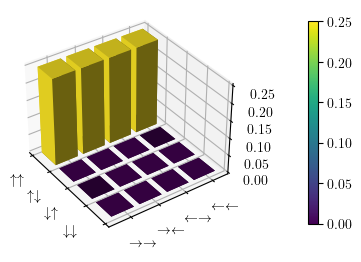
\includegraphics[width=0.6\textwidth]{imgs/wigner-desargues-2-2-s1.png}
      \caption{Función de Wigner del estado
        $\ket{\uparrow\uparrow}$.}
      \label{fig:wigner-desargues-2-2-s1}
    \end{figure}

    \begin{figure}[!ht]
      \centering
      %\scalebox{0.7}{
      %  %% Creator: Matplotlib, PGF backend
%%
%% To include the figure in your LaTeX document, write
%%   \input{<filename>.pgf}
%%
%% Make sure the required packages are loaded in your preamble
%%   \usepackage{pgf}
%%
%% Also ensure that all the required font packages are loaded; for instance,
%% the lmodern package is sometimes necessary when using math font.
%%   \usepackage{lmodern}
%%
%% Figures using additional raster images can only be included by \input if
%% they are in the same directory as the main LaTeX file. For loading figures
%% from other directories you can use the `import` package
%%   \usepackage{import}
%%
%% and then include the figures with
%%   \import{<path to file>}{<filename>.pgf}
%%
%% Matplotlib used the following preamble
%%   
%%   \makeatletter\@ifpackageloaded{underscore}{}{\usepackage[strings]{underscore}}\makeatother
%%
\begingroup%
\makeatletter%
\begin{pgfpicture}%
\pgfpathrectangle{\pgfpointorigin}{\pgfqpoint{4.500000in}{3.500000in}}%
\pgfusepath{use as bounding box, clip}%
\begin{pgfscope}%
\pgfsetbuttcap%
\pgfsetmiterjoin%
\definecolor{currentfill}{rgb}{1.000000,1.000000,1.000000}%
\pgfsetfillcolor{currentfill}%
\pgfsetlinewidth{0.000000pt}%
\definecolor{currentstroke}{rgb}{1.000000,1.000000,1.000000}%
\pgfsetstrokecolor{currentstroke}%
\pgfsetdash{}{0pt}%
\pgfpathmoveto{\pgfqpoint{0.000000in}{0.000000in}}%
\pgfpathlineto{\pgfqpoint{4.500000in}{0.000000in}}%
\pgfpathlineto{\pgfqpoint{4.500000in}{3.500000in}}%
\pgfpathlineto{\pgfqpoint{0.000000in}{3.500000in}}%
\pgfpathlineto{\pgfqpoint{0.000000in}{0.000000in}}%
\pgfpathclose%
\pgfusepath{fill}%
\end{pgfscope}%
\begin{pgfscope}%
\pgfsetbuttcap%
\pgfsetmiterjoin%
\definecolor{currentfill}{rgb}{1.000000,1.000000,1.000000}%
\pgfsetfillcolor{currentfill}%
\pgfsetlinewidth{0.000000pt}%
\definecolor{currentstroke}{rgb}{0.000000,0.000000,0.000000}%
\pgfsetstrokecolor{currentstroke}%
\pgfsetstrokeopacity{0.000000}%
\pgfsetdash{}{0pt}%
\pgfpathmoveto{\pgfqpoint{0.562500in}{0.599063in}}%
\pgfpathlineto{\pgfqpoint{2.829375in}{0.599063in}}%
\pgfpathlineto{\pgfqpoint{2.829375in}{2.865938in}}%
\pgfpathlineto{\pgfqpoint{0.562500in}{2.865938in}}%
\pgfpathlineto{\pgfqpoint{0.562500in}{0.599063in}}%
\pgfpathclose%
\pgfusepath{fill}%
\end{pgfscope}%
\begin{pgfscope}%
\pgfsetbuttcap%
\pgfsetmiterjoin%
\definecolor{currentfill}{rgb}{0.950000,0.950000,0.950000}%
\pgfsetfillcolor{currentfill}%
\pgfsetfillopacity{0.500000}%
\pgfsetlinewidth{1.003750pt}%
\definecolor{currentstroke}{rgb}{0.950000,0.950000,0.950000}%
\pgfsetstrokecolor{currentstroke}%
\pgfsetstrokeopacity{0.500000}%
\pgfsetdash{}{0pt}%
\pgfpathmoveto{\pgfqpoint{0.747551in}{1.430281in}}%
\pgfpathlineto{\pgfqpoint{1.890368in}{1.886175in}}%
\pgfpathlineto{\pgfqpoint{1.898416in}{2.752043in}}%
\pgfpathlineto{\pgfqpoint{0.696721in}{2.321580in}}%
\pgfusepath{stroke,fill}%
\end{pgfscope}%
\begin{pgfscope}%
\pgfsetbuttcap%
\pgfsetmiterjoin%
\definecolor{currentfill}{rgb}{0.900000,0.900000,0.900000}%
\pgfsetfillcolor{currentfill}%
\pgfsetfillopacity{0.500000}%
\pgfsetlinewidth{1.003750pt}%
\definecolor{currentstroke}{rgb}{0.900000,0.900000,0.900000}%
\pgfsetstrokecolor{currentstroke}%
\pgfsetstrokeopacity{0.500000}%
\pgfsetdash{}{0pt}%
\pgfpathmoveto{\pgfqpoint{1.890368in}{1.886175in}}%
\pgfpathlineto{\pgfqpoint{2.728721in}{1.219708in}}%
\pgfpathlineto{\pgfqpoint{2.782047in}{2.121980in}}%
\pgfpathlineto{\pgfqpoint{1.898416in}{2.752043in}}%
\pgfusepath{stroke,fill}%
\end{pgfscope}%
\begin{pgfscope}%
\pgfsetbuttcap%
\pgfsetmiterjoin%
\definecolor{currentfill}{rgb}{0.925000,0.925000,0.925000}%
\pgfsetfillcolor{currentfill}%
\pgfsetfillopacity{0.500000}%
\pgfsetlinewidth{1.003750pt}%
\definecolor{currentstroke}{rgb}{0.925000,0.925000,0.925000}%
\pgfsetstrokecolor{currentstroke}%
\pgfsetstrokeopacity{0.500000}%
\pgfsetdash{}{0pt}%
\pgfpathmoveto{\pgfqpoint{0.747551in}{1.430281in}}%
\pgfpathlineto{\pgfqpoint{1.539544in}{0.686862in}}%
\pgfpathlineto{\pgfqpoint{2.728721in}{1.219708in}}%
\pgfpathlineto{\pgfqpoint{1.890368in}{1.886175in}}%
\pgfusepath{stroke,fill}%
\end{pgfscope}%
\begin{pgfscope}%
\pgfsetrectcap%
\pgfsetroundjoin%
\pgfsetlinewidth{0.803000pt}%
\definecolor{currentstroke}{rgb}{0.000000,0.000000,0.000000}%
\pgfsetstrokecolor{currentstroke}%
\pgfsetdash{}{0pt}%
\pgfpathmoveto{\pgfqpoint{0.747551in}{1.430281in}}%
\pgfpathlineto{\pgfqpoint{1.539544in}{0.686862in}}%
\pgfusepath{stroke}%
\end{pgfscope}%
\begin{pgfscope}%
\pgfsetbuttcap%
\pgfsetroundjoin%
\pgfsetlinewidth{0.803000pt}%
\definecolor{currentstroke}{rgb}{0.690196,0.690196,0.690196}%
\pgfsetstrokecolor{currentstroke}%
\pgfsetdash{}{0pt}%
\pgfpathmoveto{\pgfqpoint{0.777375in}{1.402286in}}%
\pgfpathlineto{\pgfqpoint{1.922068in}{1.860975in}}%
\pgfpathlineto{\pgfqpoint{1.931703in}{2.728309in}}%
\pgfusepath{stroke}%
\end{pgfscope}%
\begin{pgfscope}%
\pgfsetbuttcap%
\pgfsetroundjoin%
\pgfsetlinewidth{0.803000pt}%
\definecolor{currentstroke}{rgb}{0.690196,0.690196,0.690196}%
\pgfsetstrokecolor{currentstroke}%
\pgfsetdash{}{0pt}%
\pgfpathmoveto{\pgfqpoint{0.949372in}{1.240839in}}%
\pgfpathlineto{\pgfqpoint{2.104681in}{1.715803in}}%
\pgfpathlineto{\pgfqpoint{2.123652in}{2.591442in}}%
\pgfusepath{stroke}%
\end{pgfscope}%
\begin{pgfscope}%
\pgfsetbuttcap%
\pgfsetroundjoin%
\pgfsetlinewidth{0.803000pt}%
\definecolor{currentstroke}{rgb}{0.690196,0.690196,0.690196}%
\pgfsetstrokecolor{currentstroke}%
\pgfsetdash{}{0pt}%
\pgfpathmoveto{\pgfqpoint{1.127694in}{1.073453in}}%
\pgfpathlineto{\pgfqpoint{2.293654in}{1.565575in}}%
\pgfpathlineto{\pgfqpoint{2.322627in}{2.449565in}}%
\pgfusepath{stroke}%
\end{pgfscope}%
\begin{pgfscope}%
\pgfsetbuttcap%
\pgfsetroundjoin%
\pgfsetlinewidth{0.803000pt}%
\definecolor{currentstroke}{rgb}{0.690196,0.690196,0.690196}%
\pgfsetstrokecolor{currentstroke}%
\pgfsetdash{}{0pt}%
\pgfpathmoveto{\pgfqpoint{1.312698in}{0.899796in}}%
\pgfpathlineto{\pgfqpoint{2.489324in}{1.410022in}}%
\pgfpathlineto{\pgfqpoint{2.529021in}{2.302397in}}%
\pgfusepath{stroke}%
\end{pgfscope}%
\begin{pgfscope}%
\pgfsetbuttcap%
\pgfsetroundjoin%
\pgfsetlinewidth{0.803000pt}%
\definecolor{currentstroke}{rgb}{0.690196,0.690196,0.690196}%
\pgfsetstrokecolor{currentstroke}%
\pgfsetdash{}{0pt}%
\pgfpathmoveto{\pgfqpoint{1.504765in}{0.719508in}}%
\pgfpathlineto{\pgfqpoint{2.692056in}{1.248856in}}%
\pgfpathlineto{\pgfqpoint{2.743258in}{2.149638in}}%
\pgfusepath{stroke}%
\end{pgfscope}%
\begin{pgfscope}%
\pgfsetrectcap%
\pgfsetroundjoin%
\pgfsetlinewidth{0.803000pt}%
\definecolor{currentstroke}{rgb}{0.000000,0.000000,0.000000}%
\pgfsetstrokecolor{currentstroke}%
\pgfsetdash{}{0pt}%
\pgfpathmoveto{\pgfqpoint{0.787024in}{1.406153in}}%
\pgfpathlineto{\pgfqpoint{0.758053in}{1.394544in}}%
\pgfusepath{stroke}%
\end{pgfscope}%
\begin{pgfscope}%
\definecolor{textcolor}{rgb}{0.000000,0.000000,0.000000}%
\pgfsetstrokecolor{textcolor}%
\pgfsetfillcolor{textcolor}%
\pgftext[x=0.620406in,y=1.221969in,,top]{\color{textcolor}\rmfamily\fontsize{10.000000}{12.000000}\selectfont \(\displaystyle \uparrow\uparrow\)}%
\end{pgfscope}%
\begin{pgfscope}%
\pgfsetrectcap%
\pgfsetroundjoin%
\pgfsetlinewidth{0.803000pt}%
\definecolor{currentstroke}{rgb}{0.000000,0.000000,0.000000}%
\pgfsetstrokecolor{currentstroke}%
\pgfsetdash{}{0pt}%
\pgfpathmoveto{\pgfqpoint{0.959119in}{1.244846in}}%
\pgfpathlineto{\pgfqpoint{0.929852in}{1.232814in}}%
\pgfusepath{stroke}%
\end{pgfscope}%
\begin{pgfscope}%
\definecolor{textcolor}{rgb}{0.000000,0.000000,0.000000}%
\pgfsetstrokecolor{textcolor}%
\pgfsetfillcolor{textcolor}%
\pgftext[x=0.789674in,y=1.057162in,,top]{\color{textcolor}\rmfamily\fontsize{10.000000}{12.000000}\selectfont \(\displaystyle \uparrow\downarrow\)}%
\end{pgfscope}%
\begin{pgfscope}%
\pgfsetrectcap%
\pgfsetroundjoin%
\pgfsetlinewidth{0.803000pt}%
\definecolor{currentstroke}{rgb}{0.000000,0.000000,0.000000}%
\pgfsetstrokecolor{currentstroke}%
\pgfsetdash{}{0pt}%
\pgfpathmoveto{\pgfqpoint{1.137540in}{1.077609in}}%
\pgfpathlineto{\pgfqpoint{1.107975in}{1.065130in}}%
\pgfusepath{stroke}%
\end{pgfscope}%
\begin{pgfscope}%
\definecolor{textcolor}{rgb}{0.000000,0.000000,0.000000}%
\pgfsetstrokecolor{textcolor}%
\pgfsetfillcolor{textcolor}%
\pgftext[x=0.965172in,y=0.886290in,,top]{\color{textcolor}\rmfamily\fontsize{10.000000}{12.000000}\selectfont \(\displaystyle \downarrow\uparrow\)}%
\end{pgfscope}%
\begin{pgfscope}%
\pgfsetrectcap%
\pgfsetroundjoin%
\pgfsetlinewidth{0.803000pt}%
\definecolor{currentstroke}{rgb}{0.000000,0.000000,0.000000}%
\pgfsetstrokecolor{currentstroke}%
\pgfsetdash{}{0pt}%
\pgfpathmoveto{\pgfqpoint{1.322644in}{0.904109in}}%
\pgfpathlineto{\pgfqpoint{1.292778in}{0.891158in}}%
\pgfusepath{stroke}%
\end{pgfscope}%
\begin{pgfscope}%
\definecolor{textcolor}{rgb}{0.000000,0.000000,0.000000}%
\pgfsetstrokecolor{textcolor}%
\pgfsetfillcolor{textcolor}%
\pgftext[x=1.147250in,y=0.709010in,,top]{\color{textcolor}\rmfamily\fontsize{10.000000}{12.000000}\selectfont \(\displaystyle \downarrow\downarrow\)}%
\end{pgfscope}%
\begin{pgfscope}%
\pgfsetrectcap%
\pgfsetroundjoin%
\pgfsetlinewidth{0.803000pt}%
\definecolor{currentstroke}{rgb}{0.000000,0.000000,0.000000}%
\pgfsetstrokecolor{currentstroke}%
\pgfsetdash{}{0pt}%
\pgfpathmoveto{\pgfqpoint{1.514812in}{0.723987in}}%
\pgfpathlineto{\pgfqpoint{1.484644in}{0.710537in}}%
\pgfusepath{stroke}%
\end{pgfscope}%
\begin{pgfscope}%
\pgfsetrectcap%
\pgfsetroundjoin%
\pgfsetlinewidth{0.803000pt}%
\definecolor{currentstroke}{rgb}{0.000000,0.000000,0.000000}%
\pgfsetstrokecolor{currentstroke}%
\pgfsetdash{}{0pt}%
\pgfpathmoveto{\pgfqpoint{2.728721in}{1.219708in}}%
\pgfpathlineto{\pgfqpoint{1.539544in}{0.686862in}}%
\pgfusepath{stroke}%
\end{pgfscope}%
\begin{pgfscope}%
\pgfsetbuttcap%
\pgfsetroundjoin%
\pgfsetlinewidth{0.803000pt}%
\definecolor{currentstroke}{rgb}{0.690196,0.690196,0.690196}%
\pgfsetstrokecolor{currentstroke}%
\pgfsetdash{}{0pt}%
\pgfpathmoveto{\pgfqpoint{0.921077in}{2.401947in}}%
\pgfpathlineto{\pgfqpoint{0.960455in}{1.515213in}}%
\pgfpathlineto{\pgfqpoint{1.761853in}{0.786474in}}%
\pgfusepath{stroke}%
\end{pgfscope}%
\begin{pgfscope}%
\pgfsetbuttcap%
\pgfsetroundjoin%
\pgfsetlinewidth{0.803000pt}%
\definecolor{currentstroke}{rgb}{0.690196,0.690196,0.690196}%
\pgfsetstrokecolor{currentstroke}%
\pgfsetdash{}{0pt}%
\pgfpathmoveto{\pgfqpoint{1.203262in}{2.503030in}}%
\pgfpathlineto{\pgfqpoint{1.228535in}{1.622156in}}%
\pgfpathlineto{\pgfqpoint{2.041274in}{0.911677in}}%
\pgfusepath{stroke}%
\end{pgfscope}%
\begin{pgfscope}%
\pgfsetbuttcap%
\pgfsetroundjoin%
\pgfsetlinewidth{0.803000pt}%
\definecolor{currentstroke}{rgb}{0.690196,0.690196,0.690196}%
\pgfsetstrokecolor{currentstroke}%
\pgfsetdash{}{0pt}%
\pgfpathmoveto{\pgfqpoint{1.478354in}{2.601571in}}%
\pgfpathlineto{\pgfqpoint{1.490198in}{1.726539in}}%
\pgfpathlineto{\pgfqpoint{2.313468in}{1.033642in}}%
\pgfusepath{stroke}%
\end{pgfscope}%
\begin{pgfscope}%
\pgfsetbuttcap%
\pgfsetroundjoin%
\pgfsetlinewidth{0.803000pt}%
\definecolor{currentstroke}{rgb}{0.690196,0.690196,0.690196}%
\pgfsetstrokecolor{currentstroke}%
\pgfsetdash{}{0pt}%
\pgfpathmoveto{\pgfqpoint{1.746616in}{2.697666in}}%
\pgfpathlineto{\pgfqpoint{1.745671in}{1.828452in}}%
\pgfpathlineto{\pgfqpoint{2.578712in}{1.152492in}}%
\pgfusepath{stroke}%
\end{pgfscope}%
\begin{pgfscope}%
\pgfsetrectcap%
\pgfsetroundjoin%
\pgfsetlinewidth{0.803000pt}%
\definecolor{currentstroke}{rgb}{0.000000,0.000000,0.000000}%
\pgfsetstrokecolor{currentstroke}%
\pgfsetdash{}{0pt}%
\pgfpathmoveto{\pgfqpoint{1.754918in}{0.792781in}}%
\pgfpathlineto{\pgfqpoint{1.775753in}{0.773835in}}%
\pgfusepath{stroke}%
\end{pgfscope}%
\begin{pgfscope}%
\definecolor{textcolor}{rgb}{0.000000,0.000000,0.000000}%
\pgfsetstrokecolor{textcolor}%
\pgfsetfillcolor{textcolor}%
\pgftext[x=1.879436in,y=0.560550in,,top]{\color{textcolor}\rmfamily\fontsize{10.000000}{12.000000}\selectfont \(\displaystyle \rightarrow\rightarrow\)}%
\end{pgfscope}%
\begin{pgfscope}%
\pgfsetrectcap%
\pgfsetroundjoin%
\pgfsetlinewidth{0.803000pt}%
\definecolor{currentstroke}{rgb}{0.000000,0.000000,0.000000}%
\pgfsetstrokecolor{currentstroke}%
\pgfsetdash{}{0pt}%
\pgfpathmoveto{\pgfqpoint{2.034247in}{0.917820in}}%
\pgfpathlineto{\pgfqpoint{2.055356in}{0.899367in}}%
\pgfusepath{stroke}%
\end{pgfscope}%
\begin{pgfscope}%
\definecolor{textcolor}{rgb}{0.000000,0.000000,0.000000}%
\pgfsetstrokecolor{textcolor}%
\pgfsetfillcolor{textcolor}%
\pgftext[x=2.158420in,y=0.689222in,,top]{\color{textcolor}\rmfamily\fontsize{10.000000}{12.000000}\selectfont \(\displaystyle \rightarrow\leftarrow\)}%
\end{pgfscope}%
\begin{pgfscope}%
\pgfsetrectcap%
\pgfsetroundjoin%
\pgfsetlinewidth{0.803000pt}%
\definecolor{currentstroke}{rgb}{0.000000,0.000000,0.000000}%
\pgfsetstrokecolor{currentstroke}%
\pgfsetdash{}{0pt}%
\pgfpathmoveto{\pgfqpoint{2.306357in}{1.039627in}}%
\pgfpathlineto{\pgfqpoint{2.327718in}{1.021649in}}%
\pgfusepath{stroke}%
\end{pgfscope}%
\begin{pgfscope}%
\definecolor{textcolor}{rgb}{0.000000,0.000000,0.000000}%
\pgfsetstrokecolor{textcolor}%
\pgfsetfillcolor{textcolor}%
\pgftext[x=2.430160in,y=0.814552in,,top]{\color{textcolor}\rmfamily\fontsize{10.000000}{12.000000}\selectfont \(\displaystyle \leftarrow\rightarrow\)}%
\end{pgfscope}%
\begin{pgfscope}%
\pgfsetrectcap%
\pgfsetroundjoin%
\pgfsetlinewidth{0.803000pt}%
\definecolor{currentstroke}{rgb}{0.000000,0.000000,0.000000}%
\pgfsetstrokecolor{currentstroke}%
\pgfsetdash{}{0pt}%
\pgfpathmoveto{\pgfqpoint{2.571523in}{1.158326in}}%
\pgfpathlineto{\pgfqpoint{2.593117in}{1.140803in}}%
\pgfusepath{stroke}%
\end{pgfscope}%
\begin{pgfscope}%
\definecolor{textcolor}{rgb}{0.000000,0.000000,0.000000}%
\pgfsetstrokecolor{textcolor}%
\pgfsetfillcolor{textcolor}%
\pgftext[x=2.694935in,y=0.936671in,,top]{\color{textcolor}\rmfamily\fontsize{10.000000}{12.000000}\selectfont \(\displaystyle \leftarrow\leftarrow\)}%
\end{pgfscope}%
\begin{pgfscope}%
\pgfsetrectcap%
\pgfsetroundjoin%
\pgfsetlinewidth{0.803000pt}%
\definecolor{currentstroke}{rgb}{0.000000,0.000000,0.000000}%
\pgfsetstrokecolor{currentstroke}%
\pgfsetdash{}{0pt}%
\pgfpathmoveto{\pgfqpoint{2.728721in}{1.219708in}}%
\pgfpathlineto{\pgfqpoint{2.782047in}{2.121980in}}%
\pgfusepath{stroke}%
\end{pgfscope}%
\begin{pgfscope}%
\pgfsetbuttcap%
\pgfsetroundjoin%
\pgfsetlinewidth{0.803000pt}%
\definecolor{currentstroke}{rgb}{0.690196,0.690196,0.690196}%
\pgfsetstrokecolor{currentstroke}%
\pgfsetdash{}{0pt}%
\pgfpathmoveto{\pgfqpoint{2.734629in}{1.319669in}}%
\pgfpathlineto{\pgfqpoint{1.891263in}{1.982435in}}%
\pgfpathlineto{\pgfqpoint{0.741914in}{1.529134in}}%
\pgfusepath{stroke}%
\end{pgfscope}%
\begin{pgfscope}%
\pgfsetbuttcap%
\pgfsetroundjoin%
\pgfsetlinewidth{0.803000pt}%
\definecolor{currentstroke}{rgb}{0.690196,0.690196,0.690196}%
\pgfsetstrokecolor{currentstroke}%
\pgfsetdash{}{0pt}%
\pgfpathmoveto{\pgfqpoint{2.744562in}{1.487738in}}%
\pgfpathlineto{\pgfqpoint{1.892766in}{2.144093in}}%
\pgfpathlineto{\pgfqpoint{0.732439in}{1.695280in}}%
\pgfusepath{stroke}%
\end{pgfscope}%
\begin{pgfscope}%
\pgfsetbuttcap%
\pgfsetroundjoin%
\pgfsetlinewidth{0.803000pt}%
\definecolor{currentstroke}{rgb}{0.690196,0.690196,0.690196}%
\pgfsetstrokecolor{currentstroke}%
\pgfsetdash{}{0pt}%
\pgfpathmoveto{\pgfqpoint{2.754693in}{1.659152in}}%
\pgfpathlineto{\pgfqpoint{1.894296in}{2.308729in}}%
\pgfpathlineto{\pgfqpoint{0.722779in}{1.864654in}}%
\pgfusepath{stroke}%
\end{pgfscope}%
\begin{pgfscope}%
\pgfsetbuttcap%
\pgfsetroundjoin%
\pgfsetlinewidth{0.803000pt}%
\definecolor{currentstroke}{rgb}{0.690196,0.690196,0.690196}%
\pgfsetstrokecolor{currentstroke}%
\pgfsetdash{}{0pt}%
\pgfpathmoveto{\pgfqpoint{2.765028in}{1.834012in}}%
\pgfpathlineto{\pgfqpoint{1.895855in}{2.476424in}}%
\pgfpathlineto{\pgfqpoint{0.712930in}{2.037352in}}%
\pgfusepath{stroke}%
\end{pgfscope}%
\begin{pgfscope}%
\pgfsetbuttcap%
\pgfsetroundjoin%
\pgfsetlinewidth{0.803000pt}%
\definecolor{currentstroke}{rgb}{0.690196,0.690196,0.690196}%
\pgfsetstrokecolor{currentstroke}%
\pgfsetdash{}{0pt}%
\pgfpathmoveto{\pgfqpoint{2.775572in}{2.012424in}}%
\pgfpathlineto{\pgfqpoint{1.897443in}{2.647265in}}%
\pgfpathlineto{\pgfqpoint{0.702886in}{2.213472in}}%
\pgfusepath{stroke}%
\end{pgfscope}%
\begin{pgfscope}%
\pgfsetrectcap%
\pgfsetroundjoin%
\pgfsetlinewidth{0.803000pt}%
\definecolor{currentstroke}{rgb}{0.000000,0.000000,0.000000}%
\pgfsetstrokecolor{currentstroke}%
\pgfsetdash{}{0pt}%
\pgfpathmoveto{\pgfqpoint{2.727352in}{1.325388in}}%
\pgfpathlineto{\pgfqpoint{2.749211in}{1.308210in}}%
\pgfusepath{stroke}%
\end{pgfscope}%
\begin{pgfscope}%
\definecolor{textcolor}{rgb}{0.000000,0.000000,0.000000}%
\pgfsetstrokecolor{textcolor}%
\pgfsetfillcolor{textcolor}%
\pgftext[x=3.011503in,y=1.290566in,,top]{\color{textcolor}\rmfamily\fontsize{10.000000}{12.000000}\selectfont \(\displaystyle {\ensuremath{-}0.10}\)}%
\end{pgfscope}%
\begin{pgfscope}%
\pgfsetrectcap%
\pgfsetroundjoin%
\pgfsetlinewidth{0.803000pt}%
\definecolor{currentstroke}{rgb}{0.000000,0.000000,0.000000}%
\pgfsetstrokecolor{currentstroke}%
\pgfsetdash{}{0pt}%
\pgfpathmoveto{\pgfqpoint{2.737207in}{1.493406in}}%
\pgfpathlineto{\pgfqpoint{2.759301in}{1.476381in}}%
\pgfusepath{stroke}%
\end{pgfscope}%
\begin{pgfscope}%
\definecolor{textcolor}{rgb}{0.000000,0.000000,0.000000}%
\pgfsetstrokecolor{textcolor}%
\pgfsetfillcolor{textcolor}%
\pgftext[x=3.024206in,y=1.458894in,,top]{\color{textcolor}\rmfamily\fontsize{10.000000}{12.000000}\selectfont \(\displaystyle {\ensuremath{-}0.05}\)}%
\end{pgfscope}%
\begin{pgfscope}%
\pgfsetrectcap%
\pgfsetroundjoin%
\pgfsetlinewidth{0.803000pt}%
\definecolor{currentstroke}{rgb}{0.000000,0.000000,0.000000}%
\pgfsetstrokecolor{currentstroke}%
\pgfsetdash{}{0pt}%
\pgfpathmoveto{\pgfqpoint{2.747258in}{1.664765in}}%
\pgfpathlineto{\pgfqpoint{2.769592in}{1.647904in}}%
\pgfusepath{stroke}%
\end{pgfscope}%
\begin{pgfscope}%
\definecolor{textcolor}{rgb}{0.000000,0.000000,0.000000}%
\pgfsetstrokecolor{textcolor}%
\pgfsetfillcolor{textcolor}%
\pgftext[x=3.037163in,y=1.630584in,,top]{\color{textcolor}\rmfamily\fontsize{10.000000}{12.000000}\selectfont \(\displaystyle {0.00}\)}%
\end{pgfscope}%
\begin{pgfscope}%
\pgfsetrectcap%
\pgfsetroundjoin%
\pgfsetlinewidth{0.803000pt}%
\definecolor{currentstroke}{rgb}{0.000000,0.000000,0.000000}%
\pgfsetstrokecolor{currentstroke}%
\pgfsetdash{}{0pt}%
\pgfpathmoveto{\pgfqpoint{2.757511in}{1.839568in}}%
\pgfpathlineto{\pgfqpoint{2.780090in}{1.822880in}}%
\pgfusepath{stroke}%
\end{pgfscope}%
\begin{pgfscope}%
\definecolor{textcolor}{rgb}{0.000000,0.000000,0.000000}%
\pgfsetstrokecolor{textcolor}%
\pgfsetfillcolor{textcolor}%
\pgftext[x=3.050380in,y=1.805737in,,top]{\color{textcolor}\rmfamily\fontsize{10.000000}{12.000000}\selectfont \(\displaystyle {0.05}\)}%
\end{pgfscope}%
\begin{pgfscope}%
\pgfsetrectcap%
\pgfsetroundjoin%
\pgfsetlinewidth{0.803000pt}%
\definecolor{currentstroke}{rgb}{0.000000,0.000000,0.000000}%
\pgfsetstrokecolor{currentstroke}%
\pgfsetdash{}{0pt}%
\pgfpathmoveto{\pgfqpoint{2.767973in}{2.017918in}}%
\pgfpathlineto{\pgfqpoint{2.790801in}{2.001414in}}%
\pgfusepath{stroke}%
\end{pgfscope}%
\begin{pgfscope}%
\definecolor{textcolor}{rgb}{0.000000,0.000000,0.000000}%
\pgfsetstrokecolor{textcolor}%
\pgfsetfillcolor{textcolor}%
\pgftext[x=3.063867in,y=1.984459in,,top]{\color{textcolor}\rmfamily\fontsize{10.000000}{12.000000}\selectfont \(\displaystyle {0.10}\)}%
\end{pgfscope}%
\begin{pgfscope}%
\pgfpathrectangle{\pgfqpoint{0.562500in}{0.599063in}}{\pgfqpoint{2.266875in}{2.266875in}}%
\pgfusepath{clip}%
\pgfsetbuttcap%
\pgfsetroundjoin%
\definecolor{currentfill}{rgb}{0.204703,0.003737,0.252551}%
\pgfsetfillcolor{currentfill}%
\pgfsetlinewidth{0.000000pt}%
\definecolor{currentstroke}{rgb}{0.000000,0.000000,0.000000}%
\pgfsetstrokecolor{currentstroke}%
\pgfsetdash{}{0pt}%
\pgfpathmoveto{\pgfqpoint{1.408241in}{1.649932in}}%
\pgfpathlineto{\pgfqpoint{1.550735in}{1.527960in}}%
\pgfpathlineto{\pgfqpoint{1.760286in}{1.613721in}}%
\pgfpathlineto{\pgfqpoint{1.616287in}{1.733347in}}%
\pgfpathlineto{\pgfqpoint{1.408241in}{1.649932in}}%
\pgfpathclose%
\pgfusepath{fill}%
\end{pgfscope}%
\begin{pgfscope}%
\pgfpathrectangle{\pgfqpoint{0.562500in}{0.599063in}}{\pgfqpoint{2.266875in}{2.266875in}}%
\pgfusepath{clip}%
\pgfsetbuttcap%
\pgfsetroundjoin%
\definecolor{currentfill}{rgb}{0.111252,0.002031,0.137256}%
\pgfsetfillcolor{currentfill}%
\pgfsetlinewidth{0.000000pt}%
\definecolor{currentstroke}{rgb}{0.000000,0.000000,0.000000}%
\pgfsetstrokecolor{currentstroke}%
\pgfsetdash{}{0pt}%
\pgfpathmoveto{\pgfqpoint{1.400689in}{2.062414in}}%
\pgfpathlineto{\pgfqpoint{1.408241in}{1.649932in}}%
\pgfpathlineto{\pgfqpoint{1.616287in}{1.733347in}}%
\pgfpathlineto{\pgfqpoint{1.613696in}{2.143738in}}%
\pgfpathlineto{\pgfqpoint{1.400689in}{2.062414in}}%
\pgfpathclose%
\pgfusepath{fill}%
\end{pgfscope}%
\begin{pgfscope}%
\pgfpathrectangle{\pgfqpoint{0.562500in}{0.599063in}}{\pgfqpoint{2.266875in}{2.266875in}}%
\pgfusepath{clip}%
\pgfsetbuttcap%
\pgfsetroundjoin%
\definecolor{currentfill}{rgb}{0.235854,0.004305,0.290983}%
\pgfsetfillcolor{currentfill}%
\pgfsetlinewidth{0.000000pt}%
\definecolor{currentstroke}{rgb}{0.000000,0.000000,0.000000}%
\pgfsetstrokecolor{currentstroke}%
\pgfsetdash{}{0pt}%
\pgfpathmoveto{\pgfqpoint{1.613696in}{2.143738in}}%
\pgfpathlineto{\pgfqpoint{1.616287in}{1.733347in}}%
\pgfpathlineto{\pgfqpoint{1.760286in}{1.613721in}}%
\pgfpathlineto{\pgfqpoint{1.761089in}{2.027100in}}%
\pgfpathlineto{\pgfqpoint{1.613696in}{2.143738in}}%
\pgfpathclose%
\pgfusepath{fill}%
\end{pgfscope}%
\begin{pgfscope}%
\pgfpathrectangle{\pgfqpoint{0.562500in}{0.599063in}}{\pgfqpoint{2.266875in}{2.266875in}}%
\pgfusepath{clip}%
\pgfsetbuttcap%
\pgfsetroundjoin%
\definecolor{currentfill}{rgb}{0.529732,0.483284,0.076766}%
\pgfsetfillcolor{currentfill}%
\pgfsetlinewidth{0.000000pt}%
\definecolor{currentstroke}{rgb}{0.000000,0.000000,0.000000}%
\pgfsetstrokecolor{currentstroke}%
\pgfsetdash{}{0pt}%
\pgfpathmoveto{\pgfqpoint{1.666296in}{2.163820in}}%
\pgfpathlineto{\pgfqpoint{1.874144in}{2.243174in}}%
\pgfpathlineto{\pgfqpoint{2.023383in}{2.129368in}}%
\pgfpathlineto{\pgfqpoint{1.814069in}{2.047757in}}%
\pgfpathlineto{\pgfqpoint{1.666296in}{2.163820in}}%
\pgfpathclose%
\pgfusepath{fill}%
\end{pgfscope}%
\begin{pgfscope}%
\pgfpathrectangle{\pgfqpoint{0.562500in}{0.599063in}}{\pgfqpoint{2.266875in}{2.266875in}}%
\pgfusepath{clip}%
\pgfsetbuttcap%
\pgfsetroundjoin%
\definecolor{currentfill}{rgb}{0.877369,0.800439,0.127143}%
\pgfsetfillcolor{currentfill}%
\pgfsetlinewidth{0.000000pt}%
\definecolor{currentstroke}{rgb}{0.000000,0.000000,0.000000}%
\pgfsetstrokecolor{currentstroke}%
\pgfsetdash{}{0pt}%
\pgfpathmoveto{\pgfqpoint{1.666296in}{2.163820in}}%
\pgfpathlineto{\pgfqpoint{1.664850in}{2.593360in}}%
\pgfpathlineto{\pgfqpoint{1.877650in}{2.670333in}}%
\pgfpathlineto{\pgfqpoint{1.874144in}{2.243174in}}%
\pgfpathlineto{\pgfqpoint{1.666296in}{2.163820in}}%
\pgfpathclose%
\pgfusepath{fill}%
\end{pgfscope}%
\begin{pgfscope}%
\pgfpathrectangle{\pgfqpoint{0.562500in}{0.599063in}}{\pgfqpoint{2.266875in}{2.266875in}}%
\pgfusepath{clip}%
\pgfsetbuttcap%
\pgfsetroundjoin%
\definecolor{currentfill}{rgb}{0.111252,0.002031,0.137256}%
\pgfsetfillcolor{currentfill}%
\pgfsetlinewidth{0.000000pt}%
\definecolor{currentstroke}{rgb}{0.000000,0.000000,0.000000}%
\pgfsetstrokecolor{currentstroke}%
\pgfsetdash{}{0pt}%
\pgfpathmoveto{\pgfqpoint{1.400689in}{2.062414in}}%
\pgfpathlineto{\pgfqpoint{1.546504in}{1.943434in}}%
\pgfpathlineto{\pgfqpoint{1.550735in}{1.527960in}}%
\pgfpathlineto{\pgfqpoint{1.408241in}{1.649932in}}%
\pgfpathlineto{\pgfqpoint{1.400689in}{2.062414in}}%
\pgfpathclose%
\pgfusepath{fill}%
\end{pgfscope}%
\begin{pgfscope}%
\pgfpathrectangle{\pgfqpoint{0.562500in}{0.599063in}}{\pgfqpoint{2.266875in}{2.266875in}}%
\pgfusepath{clip}%
\pgfsetbuttcap%
\pgfsetroundjoin%
\definecolor{currentfill}{rgb}{0.413853,0.377565,0.059973}%
\pgfsetfillcolor{currentfill}%
\pgfsetlinewidth{0.000000pt}%
\definecolor{currentstroke}{rgb}{0.000000,0.000000,0.000000}%
\pgfsetstrokecolor{currentstroke}%
\pgfsetdash{}{0pt}%
\pgfpathmoveto{\pgfqpoint{1.874144in}{2.243174in}}%
\pgfpathlineto{\pgfqpoint{1.877650in}{2.670333in}}%
\pgfpathlineto{\pgfqpoint{2.030536in}{2.559930in}}%
\pgfpathlineto{\pgfqpoint{2.023383in}{2.129368in}}%
\pgfpathlineto{\pgfqpoint{1.874144in}{2.243174in}}%
\pgfpathclose%
\pgfusepath{fill}%
\end{pgfscope}%
\begin{pgfscope}%
\pgfpathrectangle{\pgfqpoint{0.562500in}{0.599063in}}{\pgfqpoint{2.266875in}{2.266875in}}%
\pgfusepath{clip}%
\pgfsetbuttcap%
\pgfsetroundjoin%
\definecolor{currentfill}{rgb}{0.235854,0.004305,0.290983}%
\pgfsetfillcolor{currentfill}%
\pgfsetlinewidth{0.000000pt}%
\definecolor{currentstroke}{rgb}{0.000000,0.000000,0.000000}%
\pgfsetstrokecolor{currentstroke}%
\pgfsetdash{}{0pt}%
\pgfpathmoveto{\pgfqpoint{1.546504in}{1.943434in}}%
\pgfpathlineto{\pgfqpoint{1.761089in}{2.027100in}}%
\pgfpathlineto{\pgfqpoint{1.760286in}{1.613721in}}%
\pgfpathlineto{\pgfqpoint{1.550735in}{1.527960in}}%
\pgfpathlineto{\pgfqpoint{1.546504in}{1.943434in}}%
\pgfpathclose%
\pgfusepath{fill}%
\end{pgfscope}%
\begin{pgfscope}%
\pgfpathrectangle{\pgfqpoint{0.562500in}{0.599063in}}{\pgfqpoint{2.266875in}{2.266875in}}%
\pgfusepath{clip}%
\pgfsetbuttcap%
\pgfsetroundjoin%
\definecolor{currentfill}{rgb}{0.142402,0.002599,0.175688}%
\pgfsetfillcolor{currentfill}%
\pgfsetlinewidth{0.000000pt}%
\definecolor{currentstroke}{rgb}{0.000000,0.000000,0.000000}%
\pgfsetstrokecolor{currentstroke}%
\pgfsetdash{}{0pt}%
\pgfpathmoveto{\pgfqpoint{1.400689in}{2.062414in}}%
\pgfpathlineto{\pgfqpoint{1.613696in}{2.143738in}}%
\pgfpathlineto{\pgfqpoint{1.761089in}{2.027100in}}%
\pgfpathlineto{\pgfqpoint{1.546504in}{1.943434in}}%
\pgfpathlineto{\pgfqpoint{1.400689in}{2.062414in}}%
\pgfpathclose%
\pgfusepath{fill}%
\end{pgfscope}%
\begin{pgfscope}%
\pgfpathrectangle{\pgfqpoint{0.562500in}{0.599063in}}{\pgfqpoint{2.266875in}{2.266875in}}%
\pgfusepath{clip}%
\pgfsetbuttcap%
\pgfsetroundjoin%
\definecolor{currentfill}{rgb}{0.204703,0.003737,0.252551}%
\pgfsetfillcolor{currentfill}%
\pgfsetlinewidth{0.000000pt}%
\definecolor{currentstroke}{rgb}{0.000000,0.000000,0.000000}%
\pgfsetstrokecolor{currentstroke}%
\pgfsetdash{}{0pt}%
\pgfpathmoveto{\pgfqpoint{0.870050in}{1.434146in}}%
\pgfpathlineto{\pgfqpoint{1.008391in}{1.305999in}}%
\pgfpathlineto{\pgfqpoint{1.228574in}{1.396111in}}%
\pgfpathlineto{\pgfqpoint{1.088501in}{1.521733in}}%
\pgfpathlineto{\pgfqpoint{0.870050in}{1.434146in}}%
\pgfpathclose%
\pgfusepath{fill}%
\end{pgfscope}%
\begin{pgfscope}%
\pgfpathrectangle{\pgfqpoint{0.562500in}{0.599063in}}{\pgfqpoint{2.266875in}{2.266875in}}%
\pgfusepath{clip}%
\pgfsetbuttcap%
\pgfsetroundjoin%
\definecolor{currentfill}{rgb}{0.877369,0.800439,0.127143}%
\pgfsetfillcolor{currentfill}%
\pgfsetlinewidth{0.000000pt}%
\definecolor{currentstroke}{rgb}{0.000000,0.000000,0.000000}%
\pgfsetstrokecolor{currentstroke}%
\pgfsetdash{}{0pt}%
\pgfpathmoveto{\pgfqpoint{1.666296in}{2.163820in}}%
\pgfpathlineto{\pgfqpoint{1.814069in}{2.047757in}}%
\pgfpathlineto{\pgfqpoint{1.816199in}{2.480714in}}%
\pgfpathlineto{\pgfqpoint{1.664850in}{2.593360in}}%
\pgfpathlineto{\pgfqpoint{1.666296in}{2.163820in}}%
\pgfpathclose%
\pgfusepath{fill}%
\end{pgfscope}%
\begin{pgfscope}%
\pgfpathrectangle{\pgfqpoint{0.562500in}{0.599063in}}{\pgfqpoint{2.266875in}{2.266875in}}%
\pgfusepath{clip}%
\pgfsetbuttcap%
\pgfsetroundjoin%
\definecolor{currentfill}{rgb}{0.529732,0.483284,0.076766}%
\pgfsetfillcolor{currentfill}%
\pgfsetlinewidth{0.000000pt}%
\definecolor{currentstroke}{rgb}{0.000000,0.000000,0.000000}%
\pgfsetstrokecolor{currentstroke}%
\pgfsetdash{}{0pt}%
\pgfpathmoveto{\pgfqpoint{1.851670in}{2.018225in}}%
\pgfpathlineto{\pgfqpoint{2.061350in}{2.100415in}}%
\pgfpathlineto{\pgfqpoint{2.215935in}{1.982532in}}%
\pgfpathlineto{\pgfqpoint{2.004789in}{1.897962in}}%
\pgfpathlineto{\pgfqpoint{1.851670in}{2.018225in}}%
\pgfpathclose%
\pgfusepath{fill}%
\end{pgfscope}%
\begin{pgfscope}%
\pgfpathrectangle{\pgfqpoint{0.562500in}{0.599063in}}{\pgfqpoint{2.266875in}{2.266875in}}%
\pgfusepath{clip}%
\pgfsetbuttcap%
\pgfsetroundjoin%
\definecolor{currentfill}{rgb}{0.111252,0.002031,0.137256}%
\pgfsetfillcolor{currentfill}%
\pgfsetlinewidth{0.000000pt}%
\definecolor{currentstroke}{rgb}{0.000000,0.000000,0.000000}%
\pgfsetstrokecolor{currentstroke}%
\pgfsetdash{}{0pt}%
\pgfpathmoveto{\pgfqpoint{0.849213in}{1.851867in}}%
\pgfpathlineto{\pgfqpoint{0.870050in}{1.434146in}}%
\pgfpathlineto{\pgfqpoint{1.088501in}{1.521733in}}%
\pgfpathlineto{\pgfqpoint{1.073135in}{1.937358in}}%
\pgfpathlineto{\pgfqpoint{0.849213in}{1.851867in}}%
\pgfpathclose%
\pgfusepath{fill}%
\end{pgfscope}%
\begin{pgfscope}%
\pgfpathrectangle{\pgfqpoint{0.562500in}{0.599063in}}{\pgfqpoint{2.266875in}{2.266875in}}%
\pgfusepath{clip}%
\pgfsetbuttcap%
\pgfsetroundjoin%
\definecolor{currentfill}{rgb}{0.413853,0.377565,0.059973}%
\pgfsetfillcolor{currentfill}%
\pgfsetlinewidth{0.000000pt}%
\definecolor{currentstroke}{rgb}{0.000000,0.000000,0.000000}%
\pgfsetstrokecolor{currentstroke}%
\pgfsetdash{}{0pt}%
\pgfpathmoveto{\pgfqpoint{1.814069in}{2.047757in}}%
\pgfpathlineto{\pgfqpoint{2.023383in}{2.129368in}}%
\pgfpathlineto{\pgfqpoint{2.030536in}{2.559930in}}%
\pgfpathlineto{\pgfqpoint{1.816199in}{2.480714in}}%
\pgfpathlineto{\pgfqpoint{1.814069in}{2.047757in}}%
\pgfpathclose%
\pgfusepath{fill}%
\end{pgfscope}%
\begin{pgfscope}%
\pgfpathrectangle{\pgfqpoint{0.562500in}{0.599063in}}{\pgfqpoint{2.266875in}{2.266875in}}%
\pgfusepath{clip}%
\pgfsetbuttcap%
\pgfsetroundjoin%
\definecolor{currentfill}{rgb}{0.235854,0.004305,0.290983}%
\pgfsetfillcolor{currentfill}%
\pgfsetlinewidth{0.000000pt}%
\definecolor{currentstroke}{rgb}{0.000000,0.000000,0.000000}%
\pgfsetstrokecolor{currentstroke}%
\pgfsetdash{}{0pt}%
\pgfpathmoveto{\pgfqpoint{1.073135in}{1.937358in}}%
\pgfpathlineto{\pgfqpoint{1.088501in}{1.521733in}}%
\pgfpathlineto{\pgfqpoint{1.228574in}{1.396111in}}%
\pgfpathlineto{\pgfqpoint{1.216405in}{1.814730in}}%
\pgfpathlineto{\pgfqpoint{1.073135in}{1.937358in}}%
\pgfpathclose%
\pgfusepath{fill}%
\end{pgfscope}%
\begin{pgfscope}%
\pgfpathrectangle{\pgfqpoint{0.562500in}{0.599063in}}{\pgfqpoint{2.266875in}{2.266875in}}%
\pgfusepath{clip}%
\pgfsetbuttcap%
\pgfsetroundjoin%
\definecolor{currentfill}{rgb}{0.877369,0.800439,0.127143}%
\pgfsetfillcolor{currentfill}%
\pgfsetlinewidth{0.000000pt}%
\definecolor{currentstroke}{rgb}{0.000000,0.000000,0.000000}%
\pgfsetstrokecolor{currentstroke}%
\pgfsetdash{}{0pt}%
\pgfpathmoveto{\pgfqpoint{1.851670in}{2.018225in}}%
\pgfpathlineto{\pgfqpoint{1.854726in}{2.452039in}}%
\pgfpathlineto{\pgfqpoint{2.069448in}{2.531831in}}%
\pgfpathlineto{\pgfqpoint{2.061350in}{2.100415in}}%
\pgfpathlineto{\pgfqpoint{1.851670in}{2.018225in}}%
\pgfpathclose%
\pgfusepath{fill}%
\end{pgfscope}%
\begin{pgfscope}%
\pgfpathrectangle{\pgfqpoint{0.562500in}{0.599063in}}{\pgfqpoint{2.266875in}{2.266875in}}%
\pgfusepath{clip}%
\pgfsetbuttcap%
\pgfsetroundjoin%
\definecolor{currentfill}{rgb}{0.761490,0.694720,0.110351}%
\pgfsetfillcolor{currentfill}%
\pgfsetlinewidth{0.000000pt}%
\definecolor{currentstroke}{rgb}{0.000000,0.000000,0.000000}%
\pgfsetstrokecolor{currentstroke}%
\pgfsetdash{}{0pt}%
\pgfpathmoveto{\pgfqpoint{1.664850in}{2.593360in}}%
\pgfpathlineto{\pgfqpoint{1.816199in}{2.480714in}}%
\pgfpathlineto{\pgfqpoint{2.030536in}{2.559930in}}%
\pgfpathlineto{\pgfqpoint{1.877650in}{2.670333in}}%
\pgfpathlineto{\pgfqpoint{1.664850in}{2.593360in}}%
\pgfpathclose%
\pgfusepath{fill}%
\end{pgfscope}%
\begin{pgfscope}%
\pgfpathrectangle{\pgfqpoint{0.562500in}{0.599063in}}{\pgfqpoint{2.266875in}{2.266875in}}%
\pgfusepath{clip}%
\pgfsetbuttcap%
\pgfsetroundjoin%
\definecolor{currentfill}{rgb}{0.413853,0.377565,0.059973}%
\pgfsetfillcolor{currentfill}%
\pgfsetlinewidth{0.000000pt}%
\definecolor{currentstroke}{rgb}{0.000000,0.000000,0.000000}%
\pgfsetstrokecolor{currentstroke}%
\pgfsetdash{}{0pt}%
\pgfpathmoveto{\pgfqpoint{2.061350in}{2.100415in}}%
\pgfpathlineto{\pgfqpoint{2.069448in}{2.531831in}}%
\pgfpathlineto{\pgfqpoint{2.227945in}{2.417376in}}%
\pgfpathlineto{\pgfqpoint{2.215935in}{1.982532in}}%
\pgfpathlineto{\pgfqpoint{2.061350in}{2.100415in}}%
\pgfpathclose%
\pgfusepath{fill}%
\end{pgfscope}%
\begin{pgfscope}%
\pgfpathrectangle{\pgfqpoint{0.562500in}{0.599063in}}{\pgfqpoint{2.266875in}{2.266875in}}%
\pgfusepath{clip}%
\pgfsetbuttcap%
\pgfsetroundjoin%
\definecolor{currentfill}{rgb}{0.529732,0.483284,0.076766}%
\pgfsetfillcolor{currentfill}%
\pgfsetlinewidth{0.000000pt}%
\definecolor{currentstroke}{rgb}{0.000000,0.000000,0.000000}%
\pgfsetstrokecolor{currentstroke}%
\pgfsetdash{}{0pt}%
\pgfpathmoveto{\pgfqpoint{1.128412in}{1.958462in}}%
\pgfpathlineto{\pgfqpoint{1.346775in}{2.041830in}}%
\pgfpathlineto{\pgfqpoint{1.492181in}{1.922254in}}%
\pgfpathlineto{\pgfqpoint{1.272123in}{1.836454in}}%
\pgfpathlineto{\pgfqpoint{1.128412in}{1.958462in}}%
\pgfpathclose%
\pgfusepath{fill}%
\end{pgfscope}%
\begin{pgfscope}%
\pgfpathrectangle{\pgfqpoint{0.562500in}{0.599063in}}{\pgfqpoint{2.266875in}{2.266875in}}%
\pgfusepath{clip}%
\pgfsetbuttcap%
\pgfsetroundjoin%
\definecolor{currentfill}{rgb}{0.877369,0.800439,0.127143}%
\pgfsetfillcolor{currentfill}%
\pgfsetlinewidth{0.000000pt}%
\definecolor{currentstroke}{rgb}{0.000000,0.000000,0.000000}%
\pgfsetstrokecolor{currentstroke}%
\pgfsetdash{}{0pt}%
\pgfpathmoveto{\pgfqpoint{1.128412in}{1.958462in}}%
\pgfpathlineto{\pgfqpoint{1.113690in}{2.393997in}}%
\pgfpathlineto{\pgfqpoint{1.337522in}{2.474960in}}%
\pgfpathlineto{\pgfqpoint{1.346775in}{2.041830in}}%
\pgfpathlineto{\pgfqpoint{1.128412in}{1.958462in}}%
\pgfpathclose%
\pgfusepath{fill}%
\end{pgfscope}%
\begin{pgfscope}%
\pgfpathrectangle{\pgfqpoint{0.562500in}{0.599063in}}{\pgfqpoint{2.266875in}{2.266875in}}%
\pgfusepath{clip}%
\pgfsetbuttcap%
\pgfsetroundjoin%
\definecolor{currentfill}{rgb}{0.529732,0.483284,0.076766}%
\pgfsetfillcolor{currentfill}%
\pgfsetlinewidth{0.000000pt}%
\definecolor{currentstroke}{rgb}{0.000000,0.000000,0.000000}%
\pgfsetstrokecolor{currentstroke}%
\pgfsetdash{}{0pt}%
\pgfpathmoveto{\pgfqpoint{1.583614in}{1.913153in}}%
\pgfpathlineto{\pgfqpoint{1.798595in}{1.997420in}}%
\pgfpathlineto{\pgfqpoint{1.951334in}{1.876551in}}%
\pgfpathlineto{\pgfqpoint{1.734773in}{1.789813in}}%
\pgfpathlineto{\pgfqpoint{1.583614in}{1.913153in}}%
\pgfpathclose%
\pgfusepath{fill}%
\end{pgfscope}%
\begin{pgfscope}%
\pgfpathrectangle{\pgfqpoint{0.562500in}{0.599063in}}{\pgfqpoint{2.266875in}{2.266875in}}%
\pgfusepath{clip}%
\pgfsetbuttcap%
\pgfsetroundjoin%
\definecolor{currentfill}{rgb}{0.111252,0.002031,0.137256}%
\pgfsetfillcolor{currentfill}%
\pgfsetlinewidth{0.000000pt}%
\definecolor{currentstroke}{rgb}{0.000000,0.000000,0.000000}%
\pgfsetstrokecolor{currentstroke}%
\pgfsetdash{}{0pt}%
\pgfpathmoveto{\pgfqpoint{0.849213in}{1.851867in}}%
\pgfpathlineto{\pgfqpoint{0.990662in}{1.726714in}}%
\pgfpathlineto{\pgfqpoint{1.008391in}{1.305999in}}%
\pgfpathlineto{\pgfqpoint{0.870050in}{1.434146in}}%
\pgfpathlineto{\pgfqpoint{0.849213in}{1.851867in}}%
\pgfpathclose%
\pgfusepath{fill}%
\end{pgfscope}%
\begin{pgfscope}%
\pgfpathrectangle{\pgfqpoint{0.562500in}{0.599063in}}{\pgfqpoint{2.266875in}{2.266875in}}%
\pgfusepath{clip}%
\pgfsetbuttcap%
\pgfsetroundjoin%
\definecolor{currentfill}{rgb}{0.413853,0.377565,0.059973}%
\pgfsetfillcolor{currentfill}%
\pgfsetlinewidth{0.000000pt}%
\definecolor{currentstroke}{rgb}{0.000000,0.000000,0.000000}%
\pgfsetstrokecolor{currentstroke}%
\pgfsetdash{}{0pt}%
\pgfpathmoveto{\pgfqpoint{1.346775in}{2.041830in}}%
\pgfpathlineto{\pgfqpoint{1.337522in}{2.474960in}}%
\pgfpathlineto{\pgfqpoint{1.486386in}{2.358821in}}%
\pgfpathlineto{\pgfqpoint{1.492181in}{1.922254in}}%
\pgfpathlineto{\pgfqpoint{1.346775in}{2.041830in}}%
\pgfpathclose%
\pgfusepath{fill}%
\end{pgfscope}%
\begin{pgfscope}%
\pgfpathrectangle{\pgfqpoint{0.562500in}{0.599063in}}{\pgfqpoint{2.266875in}{2.266875in}}%
\pgfusepath{clip}%
\pgfsetbuttcap%
\pgfsetroundjoin%
\definecolor{currentfill}{rgb}{0.235854,0.004305,0.290983}%
\pgfsetfillcolor{currentfill}%
\pgfsetlinewidth{0.000000pt}%
\definecolor{currentstroke}{rgb}{0.000000,0.000000,0.000000}%
\pgfsetstrokecolor{currentstroke}%
\pgfsetdash{}{0pt}%
\pgfpathmoveto{\pgfqpoint{0.990662in}{1.726714in}}%
\pgfpathlineto{\pgfqpoint{1.216405in}{1.814730in}}%
\pgfpathlineto{\pgfqpoint{1.228574in}{1.396111in}}%
\pgfpathlineto{\pgfqpoint{1.008391in}{1.305999in}}%
\pgfpathlineto{\pgfqpoint{0.990662in}{1.726714in}}%
\pgfpathclose%
\pgfusepath{fill}%
\end{pgfscope}%
\begin{pgfscope}%
\pgfpathrectangle{\pgfqpoint{0.562500in}{0.599063in}}{\pgfqpoint{2.266875in}{2.266875in}}%
\pgfusepath{clip}%
\pgfsetbuttcap%
\pgfsetroundjoin%
\definecolor{currentfill}{rgb}{0.877369,0.800439,0.127143}%
\pgfsetfillcolor{currentfill}%
\pgfsetlinewidth{0.000000pt}%
\definecolor{currentstroke}{rgb}{0.000000,0.000000,0.000000}%
\pgfsetstrokecolor{currentstroke}%
\pgfsetdash{}{0pt}%
\pgfpathmoveto{\pgfqpoint{1.851670in}{2.018225in}}%
\pgfpathlineto{\pgfqpoint{2.004789in}{1.897962in}}%
\pgfpathlineto{\pgfqpoint{2.011688in}{2.335217in}}%
\pgfpathlineto{\pgfqpoint{1.854726in}{2.452039in}}%
\pgfpathlineto{\pgfqpoint{1.851670in}{2.018225in}}%
\pgfpathclose%
\pgfusepath{fill}%
\end{pgfscope}%
\begin{pgfscope}%
\pgfpathrectangle{\pgfqpoint{0.562500in}{0.599063in}}{\pgfqpoint{2.266875in}{2.266875in}}%
\pgfusepath{clip}%
\pgfsetbuttcap%
\pgfsetroundjoin%
\definecolor{currentfill}{rgb}{0.877369,0.800439,0.127143}%
\pgfsetfillcolor{currentfill}%
\pgfsetlinewidth{0.000000pt}%
\definecolor{currentstroke}{rgb}{0.000000,0.000000,0.000000}%
\pgfsetstrokecolor{currentstroke}%
\pgfsetdash{}{0pt}%
\pgfpathmoveto{\pgfqpoint{1.583614in}{1.913153in}}%
\pgfpathlineto{\pgfqpoint{1.580076in}{2.349978in}}%
\pgfpathlineto{\pgfqpoint{1.800359in}{2.431836in}}%
\pgfpathlineto{\pgfqpoint{1.798595in}{1.997420in}}%
\pgfpathlineto{\pgfqpoint{1.583614in}{1.913153in}}%
\pgfpathclose%
\pgfusepath{fill}%
\end{pgfscope}%
\begin{pgfscope}%
\pgfpathrectangle{\pgfqpoint{0.562500in}{0.599063in}}{\pgfqpoint{2.266875in}{2.266875in}}%
\pgfusepath{clip}%
\pgfsetbuttcap%
\pgfsetroundjoin%
\definecolor{currentfill}{rgb}{0.529732,0.483284,0.076766}%
\pgfsetfillcolor{currentfill}%
\pgfsetlinewidth{0.000000pt}%
\definecolor{currentstroke}{rgb}{0.000000,0.000000,0.000000}%
\pgfsetstrokecolor{currentstroke}%
\pgfsetdash{}{0pt}%
\pgfpathmoveto{\pgfqpoint{2.043763in}{1.867351in}}%
\pgfpathlineto{\pgfqpoint{2.255275in}{1.952532in}}%
\pgfpathlineto{\pgfqpoint{2.415497in}{1.830350in}}%
\pgfpathlineto{\pgfqpoint{2.202524in}{1.742658in}}%
\pgfpathlineto{\pgfqpoint{2.043763in}{1.867351in}}%
\pgfpathclose%
\pgfusepath{fill}%
\end{pgfscope}%
\begin{pgfscope}%
\pgfpathrectangle{\pgfqpoint{0.562500in}{0.599063in}}{\pgfqpoint{2.266875in}{2.266875in}}%
\pgfusepath{clip}%
\pgfsetbuttcap%
\pgfsetroundjoin%
\definecolor{currentfill}{rgb}{0.413853,0.377565,0.059973}%
\pgfsetfillcolor{currentfill}%
\pgfsetlinewidth{0.000000pt}%
\definecolor{currentstroke}{rgb}{0.000000,0.000000,0.000000}%
\pgfsetstrokecolor{currentstroke}%
\pgfsetdash{}{0pt}%
\pgfpathmoveto{\pgfqpoint{2.004789in}{1.897962in}}%
\pgfpathlineto{\pgfqpoint{2.215935in}{1.982532in}}%
\pgfpathlineto{\pgfqpoint{2.227945in}{2.417376in}}%
\pgfpathlineto{\pgfqpoint{2.011688in}{2.335217in}}%
\pgfpathlineto{\pgfqpoint{2.004789in}{1.897962in}}%
\pgfpathclose%
\pgfusepath{fill}%
\end{pgfscope}%
\begin{pgfscope}%
\pgfpathrectangle{\pgfqpoint{0.562500in}{0.599063in}}{\pgfqpoint{2.266875in}{2.266875in}}%
\pgfusepath{clip}%
\pgfsetbuttcap%
\pgfsetroundjoin%
\definecolor{currentfill}{rgb}{0.413853,0.377565,0.059973}%
\pgfsetfillcolor{currentfill}%
\pgfsetlinewidth{0.000000pt}%
\definecolor{currentstroke}{rgb}{0.000000,0.000000,0.000000}%
\pgfsetstrokecolor{currentstroke}%
\pgfsetdash{}{0pt}%
\pgfpathmoveto{\pgfqpoint{1.798595in}{1.997420in}}%
\pgfpathlineto{\pgfqpoint{1.800359in}{2.431836in}}%
\pgfpathlineto{\pgfqpoint{1.956921in}{2.314411in}}%
\pgfpathlineto{\pgfqpoint{1.951334in}{1.876551in}}%
\pgfpathlineto{\pgfqpoint{1.798595in}{1.997420in}}%
\pgfpathclose%
\pgfusepath{fill}%
\end{pgfscope}%
\begin{pgfscope}%
\pgfpathrectangle{\pgfqpoint{0.562500in}{0.599063in}}{\pgfqpoint{2.266875in}{2.266875in}}%
\pgfusepath{clip}%
\pgfsetbuttcap%
\pgfsetroundjoin%
\definecolor{currentfill}{rgb}{0.142402,0.002599,0.175688}%
\pgfsetfillcolor{currentfill}%
\pgfsetlinewidth{0.000000pt}%
\definecolor{currentstroke}{rgb}{0.000000,0.000000,0.000000}%
\pgfsetstrokecolor{currentstroke}%
\pgfsetdash{}{0pt}%
\pgfpathmoveto{\pgfqpoint{0.849213in}{1.851867in}}%
\pgfpathlineto{\pgfqpoint{1.073135in}{1.937358in}}%
\pgfpathlineto{\pgfqpoint{1.216405in}{1.814730in}}%
\pgfpathlineto{\pgfqpoint{0.990662in}{1.726714in}}%
\pgfpathlineto{\pgfqpoint{0.849213in}{1.851867in}}%
\pgfpathclose%
\pgfusepath{fill}%
\end{pgfscope}%
\begin{pgfscope}%
\pgfpathrectangle{\pgfqpoint{0.562500in}{0.599063in}}{\pgfqpoint{2.266875in}{2.266875in}}%
\pgfusepath{clip}%
\pgfsetbuttcap%
\pgfsetroundjoin%
\definecolor{currentfill}{rgb}{0.877369,0.800439,0.127143}%
\pgfsetfillcolor{currentfill}%
\pgfsetlinewidth{0.000000pt}%
\definecolor{currentstroke}{rgb}{0.000000,0.000000,0.000000}%
\pgfsetstrokecolor{currentstroke}%
\pgfsetdash{}{0pt}%
\pgfpathmoveto{\pgfqpoint{2.043763in}{1.867351in}}%
\pgfpathlineto{\pgfqpoint{2.051657in}{2.305469in}}%
\pgfpathlineto{\pgfqpoint{2.268298in}{2.388237in}}%
\pgfpathlineto{\pgfqpoint{2.255275in}{1.952532in}}%
\pgfpathlineto{\pgfqpoint{2.043763in}{1.867351in}}%
\pgfpathclose%
\pgfusepath{fill}%
\end{pgfscope}%
\begin{pgfscope}%
\pgfpathrectangle{\pgfqpoint{0.562500in}{0.599063in}}{\pgfqpoint{2.266875in}{2.266875in}}%
\pgfusepath{clip}%
\pgfsetbuttcap%
\pgfsetroundjoin%
\definecolor{currentfill}{rgb}{0.761490,0.694720,0.110351}%
\pgfsetfillcolor{currentfill}%
\pgfsetlinewidth{0.000000pt}%
\definecolor{currentstroke}{rgb}{0.000000,0.000000,0.000000}%
\pgfsetstrokecolor{currentstroke}%
\pgfsetdash{}{0pt}%
\pgfpathmoveto{\pgfqpoint{1.854726in}{2.452039in}}%
\pgfpathlineto{\pgfqpoint{2.011688in}{2.335217in}}%
\pgfpathlineto{\pgfqpoint{2.227945in}{2.417376in}}%
\pgfpathlineto{\pgfqpoint{2.069448in}{2.531831in}}%
\pgfpathlineto{\pgfqpoint{1.854726in}{2.452039in}}%
\pgfpathclose%
\pgfusepath{fill}%
\end{pgfscope}%
\begin{pgfscope}%
\pgfpathrectangle{\pgfqpoint{0.562500in}{0.599063in}}{\pgfqpoint{2.266875in}{2.266875in}}%
\pgfusepath{clip}%
\pgfsetbuttcap%
\pgfsetroundjoin%
\definecolor{currentfill}{rgb}{0.877369,0.800439,0.127143}%
\pgfsetfillcolor{currentfill}%
\pgfsetlinewidth{0.000000pt}%
\definecolor{currentstroke}{rgb}{0.000000,0.000000,0.000000}%
\pgfsetstrokecolor{currentstroke}%
\pgfsetdash{}{0pt}%
\pgfpathmoveto{\pgfqpoint{1.128412in}{1.958462in}}%
\pgfpathlineto{\pgfqpoint{1.272123in}{1.836454in}}%
\pgfpathlineto{\pgfqpoint{1.260770in}{2.275437in}}%
\pgfpathlineto{\pgfqpoint{1.113690in}{2.393997in}}%
\pgfpathlineto{\pgfqpoint{1.128412in}{1.958462in}}%
\pgfpathclose%
\pgfusepath{fill}%
\end{pgfscope}%
\begin{pgfscope}%
\pgfpathrectangle{\pgfqpoint{0.562500in}{0.599063in}}{\pgfqpoint{2.266875in}{2.266875in}}%
\pgfusepath{clip}%
\pgfsetbuttcap%
\pgfsetroundjoin%
\definecolor{currentfill}{rgb}{0.204703,0.003737,0.252551}%
\pgfsetfillcolor{currentfill}%
\pgfsetlinewidth{0.000000pt}%
\definecolor{currentstroke}{rgb}{0.000000,0.000000,0.000000}%
\pgfsetstrokecolor{currentstroke}%
\pgfsetdash{}{0pt}%
\pgfpathmoveto{\pgfqpoint{1.964040in}{1.174181in}}%
\pgfpathlineto{\pgfqpoint{2.122680in}{1.038390in}}%
\pgfpathlineto{\pgfqpoint{2.337878in}{1.133890in}}%
\pgfpathlineto{\pgfqpoint{2.177735in}{1.266928in}}%
\pgfpathlineto{\pgfqpoint{1.964040in}{1.174181in}}%
\pgfpathclose%
\pgfusepath{fill}%
\end{pgfscope}%
\begin{pgfscope}%
\pgfpathrectangle{\pgfqpoint{0.562500in}{0.599063in}}{\pgfqpoint{2.266875in}{2.266875in}}%
\pgfusepath{clip}%
\pgfsetbuttcap%
\pgfsetroundjoin%
\definecolor{currentfill}{rgb}{0.413853,0.377565,0.059973}%
\pgfsetfillcolor{currentfill}%
\pgfsetlinewidth{0.000000pt}%
\definecolor{currentstroke}{rgb}{0.000000,0.000000,0.000000}%
\pgfsetstrokecolor{currentstroke}%
\pgfsetdash{}{0pt}%
\pgfpathmoveto{\pgfqpoint{2.255275in}{1.952532in}}%
\pgfpathlineto{\pgfqpoint{2.268298in}{2.388237in}}%
\pgfpathlineto{\pgfqpoint{2.432720in}{2.269504in}}%
\pgfpathlineto{\pgfqpoint{2.415497in}{1.830350in}}%
\pgfpathlineto{\pgfqpoint{2.255275in}{1.952532in}}%
\pgfpathclose%
\pgfusepath{fill}%
\end{pgfscope}%
\begin{pgfscope}%
\pgfpathrectangle{\pgfqpoint{0.562500in}{0.599063in}}{\pgfqpoint{2.266875in}{2.266875in}}%
\pgfusepath{clip}%
\pgfsetbuttcap%
\pgfsetroundjoin%
\definecolor{currentfill}{rgb}{0.529732,0.483284,0.076766}%
\pgfsetfillcolor{currentfill}%
\pgfsetlinewidth{0.000000pt}%
\definecolor{currentstroke}{rgb}{0.000000,0.000000,0.000000}%
\pgfsetstrokecolor{currentstroke}%
\pgfsetdash{}{0pt}%
\pgfpathmoveto{\pgfqpoint{1.308706in}{1.805395in}}%
\pgfpathlineto{\pgfqpoint{1.529189in}{1.891819in}}%
\pgfpathlineto{\pgfqpoint{1.679937in}{1.767850in}}%
\pgfpathlineto{\pgfqpoint{1.457751in}{1.678858in}}%
\pgfpathlineto{\pgfqpoint{1.308706in}{1.805395in}}%
\pgfpathclose%
\pgfusepath{fill}%
\end{pgfscope}%
\begin{pgfscope}%
\pgfpathrectangle{\pgfqpoint{0.562500in}{0.599063in}}{\pgfqpoint{2.266875in}{2.266875in}}%
\pgfusepath{clip}%
\pgfsetbuttcap%
\pgfsetroundjoin%
\definecolor{currentfill}{rgb}{0.413853,0.377565,0.059973}%
\pgfsetfillcolor{currentfill}%
\pgfsetlinewidth{0.000000pt}%
\definecolor{currentstroke}{rgb}{0.000000,0.000000,0.000000}%
\pgfsetstrokecolor{currentstroke}%
\pgfsetdash{}{0pt}%
\pgfpathmoveto{\pgfqpoint{1.272123in}{1.836454in}}%
\pgfpathlineto{\pgfqpoint{1.492181in}{1.922254in}}%
\pgfpathlineto{\pgfqpoint{1.486386in}{2.358821in}}%
\pgfpathlineto{\pgfqpoint{1.260770in}{2.275437in}}%
\pgfpathlineto{\pgfqpoint{1.272123in}{1.836454in}}%
\pgfpathclose%
\pgfusepath{fill}%
\end{pgfscope}%
\begin{pgfscope}%
\pgfpathrectangle{\pgfqpoint{0.562500in}{0.599063in}}{\pgfqpoint{2.266875in}{2.266875in}}%
\pgfusepath{clip}%
\pgfsetbuttcap%
\pgfsetroundjoin%
\definecolor{currentfill}{rgb}{0.111252,0.002031,0.137256}%
\pgfsetfillcolor{currentfill}%
\pgfsetlinewidth{0.000000pt}%
\definecolor{currentstroke}{rgb}{0.000000,0.000000,0.000000}%
\pgfsetstrokecolor{currentstroke}%
\pgfsetdash{}{0pt}%
\pgfpathmoveto{\pgfqpoint{1.969990in}{1.597884in}}%
\pgfpathlineto{\pgfqpoint{1.964040in}{1.174181in}}%
\pgfpathlineto{\pgfqpoint{2.177735in}{1.266928in}}%
\pgfpathlineto{\pgfqpoint{2.188922in}{1.688538in}}%
\pgfpathlineto{\pgfqpoint{1.969990in}{1.597884in}}%
\pgfpathclose%
\pgfusepath{fill}%
\end{pgfscope}%
\begin{pgfscope}%
\pgfpathrectangle{\pgfqpoint{0.562500in}{0.599063in}}{\pgfqpoint{2.266875in}{2.266875in}}%
\pgfusepath{clip}%
\pgfsetbuttcap%
\pgfsetroundjoin%
\definecolor{currentfill}{rgb}{0.877369,0.800439,0.127143}%
\pgfsetfillcolor{currentfill}%
\pgfsetlinewidth{0.000000pt}%
\definecolor{currentstroke}{rgb}{0.000000,0.000000,0.000000}%
\pgfsetstrokecolor{currentstroke}%
\pgfsetdash{}{0pt}%
\pgfpathmoveto{\pgfqpoint{1.583614in}{1.913153in}}%
\pgfpathlineto{\pgfqpoint{1.734773in}{1.789813in}}%
\pgfpathlineto{\pgfqpoint{1.734979in}{2.230092in}}%
\pgfpathlineto{\pgfqpoint{1.580076in}{2.349978in}}%
\pgfpathlineto{\pgfqpoint{1.583614in}{1.913153in}}%
\pgfpathclose%
\pgfusepath{fill}%
\end{pgfscope}%
\begin{pgfscope}%
\pgfpathrectangle{\pgfqpoint{0.562500in}{0.599063in}}{\pgfqpoint{2.266875in}{2.266875in}}%
\pgfusepath{clip}%
\pgfsetbuttcap%
\pgfsetroundjoin%
\definecolor{currentfill}{rgb}{0.877369,0.800439,0.127143}%
\pgfsetfillcolor{currentfill}%
\pgfsetlinewidth{0.000000pt}%
\definecolor{currentstroke}{rgb}{0.000000,0.000000,0.000000}%
\pgfsetstrokecolor{currentstroke}%
\pgfsetdash{}{0pt}%
\pgfpathmoveto{\pgfqpoint{1.308706in}{1.805395in}}%
\pgfpathlineto{\pgfqpoint{1.298228in}{2.245242in}}%
\pgfpathlineto{\pgfqpoint{1.524291in}{2.329248in}}%
\pgfpathlineto{\pgfqpoint{1.529189in}{1.891819in}}%
\pgfpathlineto{\pgfqpoint{1.308706in}{1.805395in}}%
\pgfpathclose%
\pgfusepath{fill}%
\end{pgfscope}%
\begin{pgfscope}%
\pgfpathrectangle{\pgfqpoint{0.562500in}{0.599063in}}{\pgfqpoint{2.266875in}{2.266875in}}%
\pgfusepath{clip}%
\pgfsetbuttcap%
\pgfsetroundjoin%
\definecolor{currentfill}{rgb}{0.529732,0.483284,0.076766}%
\pgfsetfillcolor{currentfill}%
\pgfsetlinewidth{0.000000pt}%
\definecolor{currentstroke}{rgb}{0.000000,0.000000,0.000000}%
\pgfsetstrokecolor{currentstroke}%
\pgfsetdash{}{0pt}%
\pgfpathmoveto{\pgfqpoint{1.773256in}{1.758412in}}%
\pgfpathlineto{\pgfqpoint{1.990212in}{1.845785in}}%
\pgfpathlineto{\pgfqpoint{2.148593in}{1.720451in}}%
\pgfpathlineto{\pgfqpoint{1.930057in}{1.630468in}}%
\pgfpathlineto{\pgfqpoint{1.773256in}{1.758412in}}%
\pgfpathclose%
\pgfusepath{fill}%
\end{pgfscope}%
\begin{pgfscope}%
\pgfpathrectangle{\pgfqpoint{0.562500in}{0.599063in}}{\pgfqpoint{2.266875in}{2.266875in}}%
\pgfusepath{clip}%
\pgfsetbuttcap%
\pgfsetroundjoin%
\definecolor{currentfill}{rgb}{0.761490,0.694720,0.110351}%
\pgfsetfillcolor{currentfill}%
\pgfsetlinewidth{0.000000pt}%
\definecolor{currentstroke}{rgb}{0.000000,0.000000,0.000000}%
\pgfsetstrokecolor{currentstroke}%
\pgfsetdash{}{0pt}%
\pgfpathmoveto{\pgfqpoint{1.113690in}{2.393997in}}%
\pgfpathlineto{\pgfqpoint{1.260770in}{2.275437in}}%
\pgfpathlineto{\pgfqpoint{1.486386in}{2.358821in}}%
\pgfpathlineto{\pgfqpoint{1.337522in}{2.474960in}}%
\pgfpathlineto{\pgfqpoint{1.113690in}{2.393997in}}%
\pgfpathclose%
\pgfusepath{fill}%
\end{pgfscope}%
\begin{pgfscope}%
\pgfpathrectangle{\pgfqpoint{0.562500in}{0.599063in}}{\pgfqpoint{2.266875in}{2.266875in}}%
\pgfusepath{clip}%
\pgfsetbuttcap%
\pgfsetroundjoin%
\definecolor{currentfill}{rgb}{0.235854,0.004305,0.290983}%
\pgfsetfillcolor{currentfill}%
\pgfsetlinewidth{0.000000pt}%
\definecolor{currentstroke}{rgb}{0.000000,0.000000,0.000000}%
\pgfsetstrokecolor{currentstroke}%
\pgfsetdash{}{0pt}%
\pgfpathmoveto{\pgfqpoint{2.188922in}{1.688538in}}%
\pgfpathlineto{\pgfqpoint{2.177735in}{1.266928in}}%
\pgfpathlineto{\pgfqpoint{2.337878in}{1.133890in}}%
\pgfpathlineto{\pgfqpoint{2.353264in}{1.558487in}}%
\pgfpathlineto{\pgfqpoint{2.188922in}{1.688538in}}%
\pgfpathclose%
\pgfusepath{fill}%
\end{pgfscope}%
\begin{pgfscope}%
\pgfpathrectangle{\pgfqpoint{0.562500in}{0.599063in}}{\pgfqpoint{2.266875in}{2.266875in}}%
\pgfusepath{clip}%
\pgfsetbuttcap%
\pgfsetroundjoin%
\definecolor{currentfill}{rgb}{0.413853,0.377565,0.059973}%
\pgfsetfillcolor{currentfill}%
\pgfsetlinewidth{0.000000pt}%
\definecolor{currentstroke}{rgb}{0.000000,0.000000,0.000000}%
\pgfsetstrokecolor{currentstroke}%
\pgfsetdash{}{0pt}%
\pgfpathmoveto{\pgfqpoint{1.734773in}{1.789813in}}%
\pgfpathlineto{\pgfqpoint{1.951334in}{1.876551in}}%
\pgfpathlineto{\pgfqpoint{1.956921in}{2.314411in}}%
\pgfpathlineto{\pgfqpoint{1.734979in}{2.230092in}}%
\pgfpathlineto{\pgfqpoint{1.734773in}{1.789813in}}%
\pgfpathclose%
\pgfusepath{fill}%
\end{pgfscope}%
\begin{pgfscope}%
\pgfpathrectangle{\pgfqpoint{0.562500in}{0.599063in}}{\pgfqpoint{2.266875in}{2.266875in}}%
\pgfusepath{clip}%
\pgfsetbuttcap%
\pgfsetroundjoin%
\definecolor{currentfill}{rgb}{0.413853,0.377565,0.059973}%
\pgfsetfillcolor{currentfill}%
\pgfsetlinewidth{0.000000pt}%
\definecolor{currentstroke}{rgb}{0.000000,0.000000,0.000000}%
\pgfsetstrokecolor{currentstroke}%
\pgfsetdash{}{0pt}%
\pgfpathmoveto{\pgfqpoint{1.529189in}{1.891819in}}%
\pgfpathlineto{\pgfqpoint{1.524291in}{2.329248in}}%
\pgfpathlineto{\pgfqpoint{1.678763in}{2.208734in}}%
\pgfpathlineto{\pgfqpoint{1.679937in}{1.767850in}}%
\pgfpathlineto{\pgfqpoint{1.529189in}{1.891819in}}%
\pgfpathclose%
\pgfusepath{fill}%
\end{pgfscope}%
\begin{pgfscope}%
\pgfpathrectangle{\pgfqpoint{0.562500in}{0.599063in}}{\pgfqpoint{2.266875in}{2.266875in}}%
\pgfusepath{clip}%
\pgfsetbuttcap%
\pgfsetroundjoin%
\definecolor{currentfill}{rgb}{0.877369,0.800439,0.127143}%
\pgfsetfillcolor{currentfill}%
\pgfsetlinewidth{0.000000pt}%
\definecolor{currentstroke}{rgb}{0.000000,0.000000,0.000000}%
\pgfsetstrokecolor{currentstroke}%
\pgfsetdash{}{0pt}%
\pgfpathmoveto{\pgfqpoint{2.043763in}{1.867351in}}%
\pgfpathlineto{\pgfqpoint{2.202524in}{1.742658in}}%
\pgfpathlineto{\pgfqpoint{2.214548in}{2.184234in}}%
\pgfpathlineto{\pgfqpoint{2.051657in}{2.305469in}}%
\pgfpathlineto{\pgfqpoint{2.043763in}{1.867351in}}%
\pgfpathclose%
\pgfusepath{fill}%
\end{pgfscope}%
\begin{pgfscope}%
\pgfpathrectangle{\pgfqpoint{0.562500in}{0.599063in}}{\pgfqpoint{2.266875in}{2.266875in}}%
\pgfusepath{clip}%
\pgfsetbuttcap%
\pgfsetroundjoin%
\definecolor{currentfill}{rgb}{0.877369,0.800439,0.127143}%
\pgfsetfillcolor{currentfill}%
\pgfsetlinewidth{0.000000pt}%
\definecolor{currentstroke}{rgb}{0.000000,0.000000,0.000000}%
\pgfsetstrokecolor{currentstroke}%
\pgfsetdash{}{0pt}%
\pgfpathmoveto{\pgfqpoint{1.773256in}{1.758412in}}%
\pgfpathlineto{\pgfqpoint{1.774433in}{2.199556in}}%
\pgfpathlineto{\pgfqpoint{1.996791in}{2.284508in}}%
\pgfpathlineto{\pgfqpoint{1.990212in}{1.845785in}}%
\pgfpathlineto{\pgfqpoint{1.773256in}{1.758412in}}%
\pgfpathclose%
\pgfusepath{fill}%
\end{pgfscope}%
\begin{pgfscope}%
\pgfpathrectangle{\pgfqpoint{0.562500in}{0.599063in}}{\pgfqpoint{2.266875in}{2.266875in}}%
\pgfusepath{clip}%
\pgfsetbuttcap%
\pgfsetroundjoin%
\definecolor{currentfill}{rgb}{0.529732,0.483284,0.076766}%
\pgfsetfillcolor{currentfill}%
\pgfsetlinewidth{0.000000pt}%
\definecolor{currentstroke}{rgb}{0.000000,0.000000,0.000000}%
\pgfsetstrokecolor{currentstroke}%
\pgfsetdash{}{0pt}%
\pgfpathmoveto{\pgfqpoint{2.242947in}{1.710909in}}%
\pgfpathlineto{\pgfqpoint{2.456285in}{1.799247in}}%
\pgfpathlineto{\pgfqpoint{2.622459in}{1.672526in}}%
\pgfpathlineto{\pgfqpoint{2.407668in}{1.581534in}}%
\pgfpathlineto{\pgfqpoint{2.242947in}{1.710909in}}%
\pgfpathclose%
\pgfusepath{fill}%
\end{pgfscope}%
\begin{pgfscope}%
\pgfpathrectangle{\pgfqpoint{0.562500in}{0.599063in}}{\pgfqpoint{2.266875in}{2.266875in}}%
\pgfusepath{clip}%
\pgfsetbuttcap%
\pgfsetroundjoin%
\definecolor{currentfill}{rgb}{0.761490,0.694720,0.110351}%
\pgfsetfillcolor{currentfill}%
\pgfsetlinewidth{0.000000pt}%
\definecolor{currentstroke}{rgb}{0.000000,0.000000,0.000000}%
\pgfsetstrokecolor{currentstroke}%
\pgfsetdash{}{0pt}%
\pgfpathmoveto{\pgfqpoint{1.580076in}{2.349978in}}%
\pgfpathlineto{\pgfqpoint{1.734979in}{2.230092in}}%
\pgfpathlineto{\pgfqpoint{1.956921in}{2.314411in}}%
\pgfpathlineto{\pgfqpoint{1.800359in}{2.431836in}}%
\pgfpathlineto{\pgfqpoint{1.580076in}{2.349978in}}%
\pgfpathclose%
\pgfusepath{fill}%
\end{pgfscope}%
\begin{pgfscope}%
\pgfpathrectangle{\pgfqpoint{0.562500in}{0.599063in}}{\pgfqpoint{2.266875in}{2.266875in}}%
\pgfusepath{clip}%
\pgfsetbuttcap%
\pgfsetroundjoin%
\definecolor{currentfill}{rgb}{0.413853,0.377565,0.059973}%
\pgfsetfillcolor{currentfill}%
\pgfsetlinewidth{0.000000pt}%
\definecolor{currentstroke}{rgb}{0.000000,0.000000,0.000000}%
\pgfsetstrokecolor{currentstroke}%
\pgfsetdash{}{0pt}%
\pgfpathmoveto{\pgfqpoint{2.202524in}{1.742658in}}%
\pgfpathlineto{\pgfqpoint{2.415497in}{1.830350in}}%
\pgfpathlineto{\pgfqpoint{2.432720in}{2.269504in}}%
\pgfpathlineto{\pgfqpoint{2.214548in}{2.184234in}}%
\pgfpathlineto{\pgfqpoint{2.202524in}{1.742658in}}%
\pgfpathclose%
\pgfusepath{fill}%
\end{pgfscope}%
\begin{pgfscope}%
\pgfpathrectangle{\pgfqpoint{0.562500in}{0.599063in}}{\pgfqpoint{2.266875in}{2.266875in}}%
\pgfusepath{clip}%
\pgfsetbuttcap%
\pgfsetroundjoin%
\definecolor{currentfill}{rgb}{0.413853,0.377565,0.059973}%
\pgfsetfillcolor{currentfill}%
\pgfsetlinewidth{0.000000pt}%
\definecolor{currentstroke}{rgb}{0.000000,0.000000,0.000000}%
\pgfsetstrokecolor{currentstroke}%
\pgfsetdash{}{0pt}%
\pgfpathmoveto{\pgfqpoint{1.990212in}{1.845785in}}%
\pgfpathlineto{\pgfqpoint{1.996791in}{2.284508in}}%
\pgfpathlineto{\pgfqpoint{2.159283in}{2.162634in}}%
\pgfpathlineto{\pgfqpoint{2.148593in}{1.720451in}}%
\pgfpathlineto{\pgfqpoint{1.990212in}{1.845785in}}%
\pgfpathclose%
\pgfusepath{fill}%
\end{pgfscope}%
\begin{pgfscope}%
\pgfpathrectangle{\pgfqpoint{0.562500in}{0.599063in}}{\pgfqpoint{2.266875in}{2.266875in}}%
\pgfusepath{clip}%
\pgfsetbuttcap%
\pgfsetroundjoin%
\definecolor{currentfill}{rgb}{0.529732,0.483284,0.076766}%
\pgfsetfillcolor{currentfill}%
\pgfsetlinewidth{0.000000pt}%
\definecolor{currentstroke}{rgb}{0.000000,0.000000,0.000000}%
\pgfsetstrokecolor{currentstroke}%
\pgfsetdash{}{0pt}%
\pgfpathmoveto{\pgfqpoint{1.026678in}{1.694847in}}%
\pgfpathlineto{\pgfqpoint{1.252879in}{1.783512in}}%
\pgfpathlineto{\pgfqpoint{1.401482in}{1.656321in}}%
\pgfpathlineto{\pgfqpoint{1.173447in}{1.564987in}}%
\pgfpathlineto{\pgfqpoint{1.026678in}{1.694847in}}%
\pgfpathclose%
\pgfusepath{fill}%
\end{pgfscope}%
\begin{pgfscope}%
\pgfpathrectangle{\pgfqpoint{0.562500in}{0.599063in}}{\pgfqpoint{2.266875in}{2.266875in}}%
\pgfusepath{clip}%
\pgfsetbuttcap%
\pgfsetroundjoin%
\definecolor{currentfill}{rgb}{0.877369,0.800439,0.127143}%
\pgfsetfillcolor{currentfill}%
\pgfsetlinewidth{0.000000pt}%
\definecolor{currentstroke}{rgb}{0.000000,0.000000,0.000000}%
\pgfsetstrokecolor{currentstroke}%
\pgfsetdash{}{0pt}%
\pgfpathmoveto{\pgfqpoint{2.242947in}{1.710909in}}%
\pgfpathlineto{\pgfqpoint{2.256042in}{2.153351in}}%
\pgfpathlineto{\pgfqpoint{2.474595in}{2.239264in}}%
\pgfpathlineto{\pgfqpoint{2.456285in}{1.799247in}}%
\pgfpathlineto{\pgfqpoint{2.242947in}{1.710909in}}%
\pgfpathclose%
\pgfusepath{fill}%
\end{pgfscope}%
\begin{pgfscope}%
\pgfpathrectangle{\pgfqpoint{0.562500in}{0.599063in}}{\pgfqpoint{2.266875in}{2.266875in}}%
\pgfusepath{clip}%
\pgfsetbuttcap%
\pgfsetroundjoin%
\definecolor{currentfill}{rgb}{0.111252,0.002031,0.137256}%
\pgfsetfillcolor{currentfill}%
\pgfsetlinewidth{0.000000pt}%
\definecolor{currentstroke}{rgb}{0.000000,0.000000,0.000000}%
\pgfsetstrokecolor{currentstroke}%
\pgfsetdash{}{0pt}%
\pgfpathmoveto{\pgfqpoint{1.969990in}{1.597884in}}%
\pgfpathlineto{\pgfqpoint{2.132755in}{1.465073in}}%
\pgfpathlineto{\pgfqpoint{2.122680in}{1.038390in}}%
\pgfpathlineto{\pgfqpoint{1.964040in}{1.174181in}}%
\pgfpathlineto{\pgfqpoint{1.969990in}{1.597884in}}%
\pgfpathclose%
\pgfusepath{fill}%
\end{pgfscope}%
\begin{pgfscope}%
\pgfpathrectangle{\pgfqpoint{0.562500in}{0.599063in}}{\pgfqpoint{2.266875in}{2.266875in}}%
\pgfusepath{clip}%
\pgfsetbuttcap%
\pgfsetroundjoin%
\definecolor{currentfill}{rgb}{0.761490,0.694720,0.110351}%
\pgfsetfillcolor{currentfill}%
\pgfsetlinewidth{0.000000pt}%
\definecolor{currentstroke}{rgb}{0.000000,0.000000,0.000000}%
\pgfsetstrokecolor{currentstroke}%
\pgfsetdash{}{0pt}%
\pgfpathmoveto{\pgfqpoint{2.051657in}{2.305469in}}%
\pgfpathlineto{\pgfqpoint{2.214548in}{2.184234in}}%
\pgfpathlineto{\pgfqpoint{2.432720in}{2.269504in}}%
\pgfpathlineto{\pgfqpoint{2.268298in}{2.388237in}}%
\pgfpathlineto{\pgfqpoint{2.051657in}{2.305469in}}%
\pgfpathclose%
\pgfusepath{fill}%
\end{pgfscope}%
\begin{pgfscope}%
\pgfpathrectangle{\pgfqpoint{0.562500in}{0.599063in}}{\pgfqpoint{2.266875in}{2.266875in}}%
\pgfusepath{clip}%
\pgfsetbuttcap%
\pgfsetroundjoin%
\definecolor{currentfill}{rgb}{0.877369,0.800439,0.127143}%
\pgfsetfillcolor{currentfill}%
\pgfsetlinewidth{0.000000pt}%
\definecolor{currentstroke}{rgb}{0.000000,0.000000,0.000000}%
\pgfsetstrokecolor{currentstroke}%
\pgfsetdash{}{0pt}%
\pgfpathmoveto{\pgfqpoint{1.308706in}{1.805395in}}%
\pgfpathlineto{\pgfqpoint{1.457751in}{1.678858in}}%
\pgfpathlineto{\pgfqpoint{1.450908in}{2.122169in}}%
\pgfpathlineto{\pgfqpoint{1.298228in}{2.245242in}}%
\pgfpathlineto{\pgfqpoint{1.308706in}{1.805395in}}%
\pgfpathclose%
\pgfusepath{fill}%
\end{pgfscope}%
\begin{pgfscope}%
\pgfpathrectangle{\pgfqpoint{0.562500in}{0.599063in}}{\pgfqpoint{2.266875in}{2.266875in}}%
\pgfusepath{clip}%
\pgfsetbuttcap%
\pgfsetroundjoin%
\definecolor{currentfill}{rgb}{0.877369,0.800439,0.127143}%
\pgfsetfillcolor{currentfill}%
\pgfsetlinewidth{0.000000pt}%
\definecolor{currentstroke}{rgb}{0.000000,0.000000,0.000000}%
\pgfsetstrokecolor{currentstroke}%
\pgfsetdash{}{0pt}%
\pgfpathmoveto{\pgfqpoint{1.026678in}{1.694847in}}%
\pgfpathlineto{\pgfqpoint{1.008896in}{2.137725in}}%
\pgfpathlineto{\pgfqpoint{1.240970in}{2.223965in}}%
\pgfpathlineto{\pgfqpoint{1.252879in}{1.783512in}}%
\pgfpathlineto{\pgfqpoint{1.026678in}{1.694847in}}%
\pgfpathclose%
\pgfusepath{fill}%
\end{pgfscope}%
\begin{pgfscope}%
\pgfpathrectangle{\pgfqpoint{0.562500in}{0.599063in}}{\pgfqpoint{2.266875in}{2.266875in}}%
\pgfusepath{clip}%
\pgfsetbuttcap%
\pgfsetroundjoin%
\definecolor{currentfill}{rgb}{0.413853,0.377565,0.059973}%
\pgfsetfillcolor{currentfill}%
\pgfsetlinewidth{0.000000pt}%
\definecolor{currentstroke}{rgb}{0.000000,0.000000,0.000000}%
\pgfsetstrokecolor{currentstroke}%
\pgfsetdash{}{0pt}%
\pgfpathmoveto{\pgfqpoint{2.456285in}{1.799247in}}%
\pgfpathlineto{\pgfqpoint{2.474595in}{2.239264in}}%
\pgfpathlineto{\pgfqpoint{2.645281in}{2.116008in}}%
\pgfpathlineto{\pgfqpoint{2.622459in}{1.672526in}}%
\pgfpathlineto{\pgfqpoint{2.456285in}{1.799247in}}%
\pgfpathclose%
\pgfusepath{fill}%
\end{pgfscope}%
\begin{pgfscope}%
\pgfpathrectangle{\pgfqpoint{0.562500in}{0.599063in}}{\pgfqpoint{2.266875in}{2.266875in}}%
\pgfusepath{clip}%
\pgfsetbuttcap%
\pgfsetroundjoin%
\definecolor{currentfill}{rgb}{0.529732,0.483284,0.076766}%
\pgfsetfillcolor{currentfill}%
\pgfsetlinewidth{0.000000pt}%
\definecolor{currentstroke}{rgb}{0.000000,0.000000,0.000000}%
\pgfsetstrokecolor{currentstroke}%
\pgfsetdash{}{0pt}%
\pgfpathmoveto{\pgfqpoint{1.495705in}{1.646635in}}%
\pgfpathlineto{\pgfqpoint{1.718318in}{1.736287in}}%
\pgfpathlineto{\pgfqpoint{1.874708in}{1.607678in}}%
\pgfpathlineto{\pgfqpoint{1.650387in}{1.515312in}}%
\pgfpathlineto{\pgfqpoint{1.495705in}{1.646635in}}%
\pgfpathclose%
\pgfusepath{fill}%
\end{pgfscope}%
\begin{pgfscope}%
\pgfpathrectangle{\pgfqpoint{0.562500in}{0.599063in}}{\pgfqpoint{2.266875in}{2.266875in}}%
\pgfusepath{clip}%
\pgfsetbuttcap%
\pgfsetroundjoin%
\definecolor{currentfill}{rgb}{0.235854,0.004305,0.290983}%
\pgfsetfillcolor{currentfill}%
\pgfsetlinewidth{0.000000pt}%
\definecolor{currentstroke}{rgb}{0.000000,0.000000,0.000000}%
\pgfsetstrokecolor{currentstroke}%
\pgfsetdash{}{0pt}%
\pgfpathmoveto{\pgfqpoint{2.132755in}{1.465073in}}%
\pgfpathlineto{\pgfqpoint{2.353264in}{1.558487in}}%
\pgfpathlineto{\pgfqpoint{2.337878in}{1.133890in}}%
\pgfpathlineto{\pgfqpoint{2.122680in}{1.038390in}}%
\pgfpathlineto{\pgfqpoint{2.132755in}{1.465073in}}%
\pgfpathclose%
\pgfusepath{fill}%
\end{pgfscope}%
\begin{pgfscope}%
\pgfpathrectangle{\pgfqpoint{0.562500in}{0.599063in}}{\pgfqpoint{2.266875in}{2.266875in}}%
\pgfusepath{clip}%
\pgfsetbuttcap%
\pgfsetroundjoin%
\definecolor{currentfill}{rgb}{0.413853,0.377565,0.059973}%
\pgfsetfillcolor{currentfill}%
\pgfsetlinewidth{0.000000pt}%
\definecolor{currentstroke}{rgb}{0.000000,0.000000,0.000000}%
\pgfsetstrokecolor{currentstroke}%
\pgfsetdash{}{0pt}%
\pgfpathmoveto{\pgfqpoint{1.457751in}{1.678858in}}%
\pgfpathlineto{\pgfqpoint{1.679937in}{1.767850in}}%
\pgfpathlineto{\pgfqpoint{1.678763in}{2.208734in}}%
\pgfpathlineto{\pgfqpoint{1.450908in}{2.122169in}}%
\pgfpathlineto{\pgfqpoint{1.457751in}{1.678858in}}%
\pgfpathclose%
\pgfusepath{fill}%
\end{pgfscope}%
\begin{pgfscope}%
\pgfpathrectangle{\pgfqpoint{0.562500in}{0.599063in}}{\pgfqpoint{2.266875in}{2.266875in}}%
\pgfusepath{clip}%
\pgfsetbuttcap%
\pgfsetroundjoin%
\definecolor{currentfill}{rgb}{0.413853,0.377565,0.059973}%
\pgfsetfillcolor{currentfill}%
\pgfsetlinewidth{0.000000pt}%
\definecolor{currentstroke}{rgb}{0.000000,0.000000,0.000000}%
\pgfsetstrokecolor{currentstroke}%
\pgfsetdash{}{0pt}%
\pgfpathmoveto{\pgfqpoint{1.252879in}{1.783512in}}%
\pgfpathlineto{\pgfqpoint{1.240970in}{2.223965in}}%
\pgfpathlineto{\pgfqpoint{1.393184in}{2.100239in}}%
\pgfpathlineto{\pgfqpoint{1.401482in}{1.656321in}}%
\pgfpathlineto{\pgfqpoint{1.252879in}{1.783512in}}%
\pgfpathclose%
\pgfusepath{fill}%
\end{pgfscope}%
\begin{pgfscope}%
\pgfpathrectangle{\pgfqpoint{0.562500in}{0.599063in}}{\pgfqpoint{2.266875in}{2.266875in}}%
\pgfusepath{clip}%
\pgfsetbuttcap%
\pgfsetroundjoin%
\definecolor{currentfill}{rgb}{0.877369,0.800439,0.127143}%
\pgfsetfillcolor{currentfill}%
\pgfsetlinewidth{0.000000pt}%
\definecolor{currentstroke}{rgb}{0.000000,0.000000,0.000000}%
\pgfsetstrokecolor{currentstroke}%
\pgfsetdash{}{0pt}%
\pgfpathmoveto{\pgfqpoint{1.773256in}{1.758412in}}%
\pgfpathlineto{\pgfqpoint{1.930057in}{1.630468in}}%
\pgfpathlineto{\pgfqpoint{1.935266in}{2.075080in}}%
\pgfpathlineto{\pgfqpoint{1.774433in}{2.199556in}}%
\pgfpathlineto{\pgfqpoint{1.773256in}{1.758412in}}%
\pgfpathclose%
\pgfusepath{fill}%
\end{pgfscope}%
\begin{pgfscope}%
\pgfpathrectangle{\pgfqpoint{0.562500in}{0.599063in}}{\pgfqpoint{2.266875in}{2.266875in}}%
\pgfusepath{clip}%
\pgfsetbuttcap%
\pgfsetroundjoin%
\definecolor{currentfill}{rgb}{0.877369,0.800439,0.127143}%
\pgfsetfillcolor{currentfill}%
\pgfsetlinewidth{0.000000pt}%
\definecolor{currentstroke}{rgb}{0.000000,0.000000,0.000000}%
\pgfsetstrokecolor{currentstroke}%
\pgfsetdash{}{0pt}%
\pgfpathmoveto{\pgfqpoint{1.495705in}{1.646635in}}%
\pgfpathlineto{\pgfqpoint{1.489806in}{2.090814in}}%
\pgfpathlineto{\pgfqpoint{1.718109in}{2.178038in}}%
\pgfpathlineto{\pgfqpoint{1.718318in}{1.736287in}}%
\pgfpathlineto{\pgfqpoint{1.495705in}{1.646635in}}%
\pgfpathclose%
\pgfusepath{fill}%
\end{pgfscope}%
\begin{pgfscope}%
\pgfpathrectangle{\pgfqpoint{0.562500in}{0.599063in}}{\pgfqpoint{2.266875in}{2.266875in}}%
\pgfusepath{clip}%
\pgfsetbuttcap%
\pgfsetroundjoin%
\definecolor{currentfill}{rgb}{0.142402,0.002599,0.175688}%
\pgfsetfillcolor{currentfill}%
\pgfsetlinewidth{0.000000pt}%
\definecolor{currentstroke}{rgb}{0.000000,0.000000,0.000000}%
\pgfsetstrokecolor{currentstroke}%
\pgfsetdash{}{0pt}%
\pgfpathmoveto{\pgfqpoint{1.969990in}{1.597884in}}%
\pgfpathlineto{\pgfqpoint{2.188922in}{1.688538in}}%
\pgfpathlineto{\pgfqpoint{2.353264in}{1.558487in}}%
\pgfpathlineto{\pgfqpoint{2.132755in}{1.465073in}}%
\pgfpathlineto{\pgfqpoint{1.969990in}{1.597884in}}%
\pgfpathclose%
\pgfusepath{fill}%
\end{pgfscope}%
\begin{pgfscope}%
\pgfpathrectangle{\pgfqpoint{0.562500in}{0.599063in}}{\pgfqpoint{2.266875in}{2.266875in}}%
\pgfusepath{clip}%
\pgfsetbuttcap%
\pgfsetroundjoin%
\definecolor{currentfill}{rgb}{0.761490,0.694720,0.110351}%
\pgfsetfillcolor{currentfill}%
\pgfsetlinewidth{0.000000pt}%
\definecolor{currentstroke}{rgb}{0.000000,0.000000,0.000000}%
\pgfsetstrokecolor{currentstroke}%
\pgfsetdash{}{0pt}%
\pgfpathmoveto{\pgfqpoint{1.298228in}{2.245242in}}%
\pgfpathlineto{\pgfqpoint{1.450908in}{2.122169in}}%
\pgfpathlineto{\pgfqpoint{1.678763in}{2.208734in}}%
\pgfpathlineto{\pgfqpoint{1.524291in}{2.329248in}}%
\pgfpathlineto{\pgfqpoint{1.298228in}{2.245242in}}%
\pgfpathclose%
\pgfusepath{fill}%
\end{pgfscope}%
\begin{pgfscope}%
\pgfpathrectangle{\pgfqpoint{0.562500in}{0.599063in}}{\pgfqpoint{2.266875in}{2.266875in}}%
\pgfusepath{clip}%
\pgfsetbuttcap%
\pgfsetroundjoin%
\definecolor{currentfill}{rgb}{0.204703,0.003737,0.252551}%
\pgfsetfillcolor{currentfill}%
\pgfsetlinewidth{0.000000pt}%
\definecolor{currentstroke}{rgb}{0.000000,0.000000,0.000000}%
\pgfsetstrokecolor{currentstroke}%
\pgfsetdash{}{0pt}%
\pgfpathmoveto{\pgfqpoint{1.410195in}{0.933804in}}%
\pgfpathlineto{\pgfqpoint{1.564636in}{0.790744in}}%
\pgfpathlineto{\pgfqpoint{1.791380in}{0.891367in}}%
\pgfpathlineto{\pgfqpoint{1.635182in}{1.031452in}}%
\pgfpathlineto{\pgfqpoint{1.410195in}{0.933804in}}%
\pgfpathclose%
\pgfusepath{fill}%
\end{pgfscope}%
\begin{pgfscope}%
\pgfpathrectangle{\pgfqpoint{0.562500in}{0.599063in}}{\pgfqpoint{2.266875in}{2.266875in}}%
\pgfusepath{clip}%
\pgfsetbuttcap%
\pgfsetroundjoin%
\definecolor{currentfill}{rgb}{0.413853,0.377565,0.059973}%
\pgfsetfillcolor{currentfill}%
\pgfsetlinewidth{0.000000pt}%
\definecolor{currentstroke}{rgb}{0.000000,0.000000,0.000000}%
\pgfsetstrokecolor{currentstroke}%
\pgfsetdash{}{0pt}%
\pgfpathmoveto{\pgfqpoint{1.930057in}{1.630468in}}%
\pgfpathlineto{\pgfqpoint{2.148593in}{1.720451in}}%
\pgfpathlineto{\pgfqpoint{2.159283in}{2.162634in}}%
\pgfpathlineto{\pgfqpoint{1.935266in}{2.075080in}}%
\pgfpathlineto{\pgfqpoint{1.930057in}{1.630468in}}%
\pgfpathclose%
\pgfusepath{fill}%
\end{pgfscope}%
\begin{pgfscope}%
\pgfpathrectangle{\pgfqpoint{0.562500in}{0.599063in}}{\pgfqpoint{2.266875in}{2.266875in}}%
\pgfusepath{clip}%
\pgfsetbuttcap%
\pgfsetroundjoin%
\definecolor{currentfill}{rgb}{0.413853,0.377565,0.059973}%
\pgfsetfillcolor{currentfill}%
\pgfsetlinewidth{0.000000pt}%
\definecolor{currentstroke}{rgb}{0.000000,0.000000,0.000000}%
\pgfsetstrokecolor{currentstroke}%
\pgfsetdash{}{0pt}%
\pgfpathmoveto{\pgfqpoint{1.718318in}{1.736287in}}%
\pgfpathlineto{\pgfqpoint{1.718109in}{2.178038in}}%
\pgfpathlineto{\pgfqpoint{1.878510in}{2.052897in}}%
\pgfpathlineto{\pgfqpoint{1.874708in}{1.607678in}}%
\pgfpathlineto{\pgfqpoint{1.718318in}{1.736287in}}%
\pgfpathclose%
\pgfusepath{fill}%
\end{pgfscope}%
\begin{pgfscope}%
\pgfpathrectangle{\pgfqpoint{0.562500in}{0.599063in}}{\pgfqpoint{2.266875in}{2.266875in}}%
\pgfusepath{clip}%
\pgfsetbuttcap%
\pgfsetroundjoin%
\definecolor{currentfill}{rgb}{0.877369,0.800439,0.127143}%
\pgfsetfillcolor{currentfill}%
\pgfsetlinewidth{0.000000pt}%
\definecolor{currentstroke}{rgb}{0.000000,0.000000,0.000000}%
\pgfsetstrokecolor{currentstroke}%
\pgfsetdash{}{0pt}%
\pgfpathmoveto{\pgfqpoint{2.242947in}{1.710909in}}%
\pgfpathlineto{\pgfqpoint{2.407668in}{1.581534in}}%
\pgfpathlineto{\pgfqpoint{2.425205in}{2.027447in}}%
\pgfpathlineto{\pgfqpoint{2.256042in}{2.153351in}}%
\pgfpathlineto{\pgfqpoint{2.242947in}{1.710909in}}%
\pgfpathclose%
\pgfusepath{fill}%
\end{pgfscope}%
\begin{pgfscope}%
\pgfpathrectangle{\pgfqpoint{0.562500in}{0.599063in}}{\pgfqpoint{2.266875in}{2.266875in}}%
\pgfusepath{clip}%
\pgfsetbuttcap%
\pgfsetroundjoin%
\definecolor{currentfill}{rgb}{0.111252,0.002031,0.137256}%
\pgfsetfillcolor{currentfill}%
\pgfsetlinewidth{0.000000pt}%
\definecolor{currentstroke}{rgb}{0.000000,0.000000,0.000000}%
\pgfsetstrokecolor{currentstroke}%
\pgfsetdash{}{0pt}%
\pgfpathmoveto{\pgfqpoint{1.402055in}{1.362715in}}%
\pgfpathlineto{\pgfqpoint{1.410195in}{0.933804in}}%
\pgfpathlineto{\pgfqpoint{1.635182in}{1.031452in}}%
\pgfpathlineto{\pgfqpoint{1.632855in}{1.458284in}}%
\pgfpathlineto{\pgfqpoint{1.402055in}{1.362715in}}%
\pgfpathclose%
\pgfusepath{fill}%
\end{pgfscope}%
\begin{pgfscope}%
\pgfpathrectangle{\pgfqpoint{0.562500in}{0.599063in}}{\pgfqpoint{2.266875in}{2.266875in}}%
\pgfusepath{clip}%
\pgfsetbuttcap%
\pgfsetroundjoin%
\definecolor{currentfill}{rgb}{0.761490,0.694720,0.110351}%
\pgfsetfillcolor{currentfill}%
\pgfsetlinewidth{0.000000pt}%
\definecolor{currentstroke}{rgb}{0.000000,0.000000,0.000000}%
\pgfsetstrokecolor{currentstroke}%
\pgfsetdash{}{0pt}%
\pgfpathmoveto{\pgfqpoint{1.774433in}{2.199556in}}%
\pgfpathlineto{\pgfqpoint{1.935266in}{2.075080in}}%
\pgfpathlineto{\pgfqpoint{2.159283in}{2.162634in}}%
\pgfpathlineto{\pgfqpoint{1.996791in}{2.284508in}}%
\pgfpathlineto{\pgfqpoint{1.774433in}{2.199556in}}%
\pgfpathclose%
\pgfusepath{fill}%
\end{pgfscope}%
\begin{pgfscope}%
\pgfpathrectangle{\pgfqpoint{0.562500in}{0.599063in}}{\pgfqpoint{2.266875in}{2.266875in}}%
\pgfusepath{clip}%
\pgfsetbuttcap%
\pgfsetroundjoin%
\definecolor{currentfill}{rgb}{0.877369,0.800439,0.127143}%
\pgfsetfillcolor{currentfill}%
\pgfsetlinewidth{0.000000pt}%
\definecolor{currentstroke}{rgb}{0.000000,0.000000,0.000000}%
\pgfsetstrokecolor{currentstroke}%
\pgfsetdash{}{0pt}%
\pgfpathmoveto{\pgfqpoint{1.026678in}{1.694847in}}%
\pgfpathlineto{\pgfqpoint{1.173447in}{1.564987in}}%
\pgfpathlineto{\pgfqpoint{1.159177in}{2.011337in}}%
\pgfpathlineto{\pgfqpoint{1.008896in}{2.137725in}}%
\pgfpathlineto{\pgfqpoint{1.026678in}{1.694847in}}%
\pgfpathclose%
\pgfusepath{fill}%
\end{pgfscope}%
\begin{pgfscope}%
\pgfpathrectangle{\pgfqpoint{0.562500in}{0.599063in}}{\pgfqpoint{2.266875in}{2.266875in}}%
\pgfusepath{clip}%
\pgfsetbuttcap%
\pgfsetroundjoin%
\definecolor{currentfill}{rgb}{0.413853,0.377565,0.059973}%
\pgfsetfillcolor{currentfill}%
\pgfsetlinewidth{0.000000pt}%
\definecolor{currentstroke}{rgb}{0.000000,0.000000,0.000000}%
\pgfsetstrokecolor{currentstroke}%
\pgfsetdash{}{0pt}%
\pgfpathmoveto{\pgfqpoint{2.407668in}{1.581534in}}%
\pgfpathlineto{\pgfqpoint{2.622459in}{1.672526in}}%
\pgfpathlineto{\pgfqpoint{2.645281in}{2.116008in}}%
\pgfpathlineto{\pgfqpoint{2.425205in}{2.027447in}}%
\pgfpathlineto{\pgfqpoint{2.407668in}{1.581534in}}%
\pgfpathclose%
\pgfusepath{fill}%
\end{pgfscope}%
\begin{pgfscope}%
\pgfpathrectangle{\pgfqpoint{0.562500in}{0.599063in}}{\pgfqpoint{2.266875in}{2.266875in}}%
\pgfusepath{clip}%
\pgfsetbuttcap%
\pgfsetroundjoin%
\definecolor{currentfill}{rgb}{0.529732,0.483284,0.076766}%
\pgfsetfillcolor{currentfill}%
\pgfsetlinewidth{0.000000pt}%
\definecolor{currentstroke}{rgb}{0.000000,0.000000,0.000000}%
\pgfsetstrokecolor{currentstroke}%
\pgfsetdash{}{0pt}%
\pgfpathmoveto{\pgfqpoint{1.210830in}{1.531910in}}%
\pgfpathlineto{\pgfqpoint{1.439325in}{1.623930in}}%
\pgfpathlineto{\pgfqpoint{1.593563in}{1.491915in}}%
\pgfpathlineto{\pgfqpoint{1.363225in}{1.397072in}}%
\pgfpathlineto{\pgfqpoint{1.210830in}{1.531910in}}%
\pgfpathclose%
\pgfusepath{fill}%
\end{pgfscope}%
\begin{pgfscope}%
\pgfpathrectangle{\pgfqpoint{0.562500in}{0.599063in}}{\pgfqpoint{2.266875in}{2.266875in}}%
\pgfusepath{clip}%
\pgfsetbuttcap%
\pgfsetroundjoin%
\definecolor{currentfill}{rgb}{0.235854,0.004305,0.290983}%
\pgfsetfillcolor{currentfill}%
\pgfsetlinewidth{0.000000pt}%
\definecolor{currentstroke}{rgb}{0.000000,0.000000,0.000000}%
\pgfsetstrokecolor{currentstroke}%
\pgfsetdash{}{0pt}%
\pgfpathmoveto{\pgfqpoint{1.632855in}{1.458284in}}%
\pgfpathlineto{\pgfqpoint{1.635182in}{1.031452in}}%
\pgfpathlineto{\pgfqpoint{1.791380in}{0.891367in}}%
\pgfpathlineto{\pgfqpoint{1.793056in}{1.321166in}}%
\pgfpathlineto{\pgfqpoint{1.632855in}{1.458284in}}%
\pgfpathclose%
\pgfusepath{fill}%
\end{pgfscope}%
\begin{pgfscope}%
\pgfpathrectangle{\pgfqpoint{0.562500in}{0.599063in}}{\pgfqpoint{2.266875in}{2.266875in}}%
\pgfusepath{clip}%
\pgfsetbuttcap%
\pgfsetroundjoin%
\definecolor{currentfill}{rgb}{0.413853,0.377565,0.059973}%
\pgfsetfillcolor{currentfill}%
\pgfsetlinewidth{0.000000pt}%
\definecolor{currentstroke}{rgb}{0.000000,0.000000,0.000000}%
\pgfsetstrokecolor{currentstroke}%
\pgfsetdash{}{0pt}%
\pgfpathmoveto{\pgfqpoint{1.173447in}{1.564987in}}%
\pgfpathlineto{\pgfqpoint{1.401482in}{1.656321in}}%
\pgfpathlineto{\pgfqpoint{1.393184in}{2.100239in}}%
\pgfpathlineto{\pgfqpoint{1.159177in}{2.011337in}}%
\pgfpathlineto{\pgfqpoint{1.173447in}{1.564987in}}%
\pgfpathclose%
\pgfusepath{fill}%
\end{pgfscope}%
\begin{pgfscope}%
\pgfpathrectangle{\pgfqpoint{0.562500in}{0.599063in}}{\pgfqpoint{2.266875in}{2.266875in}}%
\pgfusepath{clip}%
\pgfsetbuttcap%
\pgfsetroundjoin%
\definecolor{currentfill}{rgb}{0.761490,0.694720,0.110351}%
\pgfsetfillcolor{currentfill}%
\pgfsetlinewidth{0.000000pt}%
\definecolor{currentstroke}{rgb}{0.000000,0.000000,0.000000}%
\pgfsetstrokecolor{currentstroke}%
\pgfsetdash{}{0pt}%
\pgfpathmoveto{\pgfqpoint{2.256042in}{2.153351in}}%
\pgfpathlineto{\pgfqpoint{2.425205in}{2.027447in}}%
\pgfpathlineto{\pgfqpoint{2.645281in}{2.116008in}}%
\pgfpathlineto{\pgfqpoint{2.474595in}{2.239264in}}%
\pgfpathlineto{\pgfqpoint{2.256042in}{2.153351in}}%
\pgfpathclose%
\pgfusepath{fill}%
\end{pgfscope}%
\begin{pgfscope}%
\pgfpathrectangle{\pgfqpoint{0.562500in}{0.599063in}}{\pgfqpoint{2.266875in}{2.266875in}}%
\pgfusepath{clip}%
\pgfsetbuttcap%
\pgfsetroundjoin%
\definecolor{currentfill}{rgb}{0.877369,0.800439,0.127143}%
\pgfsetfillcolor{currentfill}%
\pgfsetlinewidth{0.000000pt}%
\definecolor{currentstroke}{rgb}{0.000000,0.000000,0.000000}%
\pgfsetstrokecolor{currentstroke}%
\pgfsetdash{}{0pt}%
\pgfpathmoveto{\pgfqpoint{1.495705in}{1.646635in}}%
\pgfpathlineto{\pgfqpoint{1.650387in}{1.515312in}}%
\pgfpathlineto{\pgfqpoint{1.648410in}{1.962965in}}%
\pgfpathlineto{\pgfqpoint{1.489806in}{2.090814in}}%
\pgfpathlineto{\pgfqpoint{1.495705in}{1.646635in}}%
\pgfpathclose%
\pgfusepath{fill}%
\end{pgfscope}%
\begin{pgfscope}%
\pgfpathrectangle{\pgfqpoint{0.562500in}{0.599063in}}{\pgfqpoint{2.266875in}{2.266875in}}%
\pgfusepath{clip}%
\pgfsetbuttcap%
\pgfsetroundjoin%
\definecolor{currentfill}{rgb}{0.877369,0.800439,0.127143}%
\pgfsetfillcolor{currentfill}%
\pgfsetlinewidth{0.000000pt}%
\definecolor{currentstroke}{rgb}{0.000000,0.000000,0.000000}%
\pgfsetstrokecolor{currentstroke}%
\pgfsetdash{}{0pt}%
\pgfpathmoveto{\pgfqpoint{1.210830in}{1.531910in}}%
\pgfpathlineto{\pgfqpoint{1.197474in}{1.979129in}}%
\pgfpathlineto{\pgfqpoint{1.431965in}{2.068716in}}%
\pgfpathlineto{\pgfqpoint{1.439325in}{1.623930in}}%
\pgfpathlineto{\pgfqpoint{1.210830in}{1.531910in}}%
\pgfpathclose%
\pgfusepath{fill}%
\end{pgfscope}%
\begin{pgfscope}%
\pgfpathrectangle{\pgfqpoint{0.562500in}{0.599063in}}{\pgfqpoint{2.266875in}{2.266875in}}%
\pgfusepath{clip}%
\pgfsetbuttcap%
\pgfsetroundjoin%
\definecolor{currentfill}{rgb}{0.529732,0.483284,0.076766}%
\pgfsetfillcolor{currentfill}%
\pgfsetlinewidth{0.000000pt}%
\definecolor{currentstroke}{rgb}{0.000000,0.000000,0.000000}%
\pgfsetstrokecolor{currentstroke}%
\pgfsetdash{}{0pt}%
\pgfpathmoveto{\pgfqpoint{1.689790in}{1.481860in}}%
\pgfpathlineto{\pgfqpoint{1.914538in}{1.574923in}}%
\pgfpathlineto{\pgfqpoint{2.076893in}{1.441408in}}%
\pgfpathlineto{\pgfqpoint{1.850435in}{1.345474in}}%
\pgfpathlineto{\pgfqpoint{1.689790in}{1.481860in}}%
\pgfpathclose%
\pgfusepath{fill}%
\end{pgfscope}%
\begin{pgfscope}%
\pgfpathrectangle{\pgfqpoint{0.562500in}{0.599063in}}{\pgfqpoint{2.266875in}{2.266875in}}%
\pgfusepath{clip}%
\pgfsetbuttcap%
\pgfsetroundjoin%
\definecolor{currentfill}{rgb}{0.761490,0.694720,0.110351}%
\pgfsetfillcolor{currentfill}%
\pgfsetlinewidth{0.000000pt}%
\definecolor{currentstroke}{rgb}{0.000000,0.000000,0.000000}%
\pgfsetstrokecolor{currentstroke}%
\pgfsetdash{}{0pt}%
\pgfpathmoveto{\pgfqpoint{1.008896in}{2.137725in}}%
\pgfpathlineto{\pgfqpoint{1.159177in}{2.011337in}}%
\pgfpathlineto{\pgfqpoint{1.393184in}{2.100239in}}%
\pgfpathlineto{\pgfqpoint{1.240970in}{2.223965in}}%
\pgfpathlineto{\pgfqpoint{1.008896in}{2.137725in}}%
\pgfpathclose%
\pgfusepath{fill}%
\end{pgfscope}%
\begin{pgfscope}%
\pgfpathrectangle{\pgfqpoint{0.562500in}{0.599063in}}{\pgfqpoint{2.266875in}{2.266875in}}%
\pgfusepath{clip}%
\pgfsetbuttcap%
\pgfsetroundjoin%
\definecolor{currentfill}{rgb}{0.413853,0.377565,0.059973}%
\pgfsetfillcolor{currentfill}%
\pgfsetlinewidth{0.000000pt}%
\definecolor{currentstroke}{rgb}{0.000000,0.000000,0.000000}%
\pgfsetstrokecolor{currentstroke}%
\pgfsetdash{}{0pt}%
\pgfpathmoveto{\pgfqpoint{1.650387in}{1.515312in}}%
\pgfpathlineto{\pgfqpoint{1.874708in}{1.607678in}}%
\pgfpathlineto{\pgfqpoint{1.878510in}{2.052897in}}%
\pgfpathlineto{\pgfqpoint{1.648410in}{1.962965in}}%
\pgfpathlineto{\pgfqpoint{1.650387in}{1.515312in}}%
\pgfpathclose%
\pgfusepath{fill}%
\end{pgfscope}%
\begin{pgfscope}%
\pgfpathrectangle{\pgfqpoint{0.562500in}{0.599063in}}{\pgfqpoint{2.266875in}{2.266875in}}%
\pgfusepath{clip}%
\pgfsetbuttcap%
\pgfsetroundjoin%
\definecolor{currentfill}{rgb}{0.413853,0.377565,0.059973}%
\pgfsetfillcolor{currentfill}%
\pgfsetlinewidth{0.000000pt}%
\definecolor{currentstroke}{rgb}{0.000000,0.000000,0.000000}%
\pgfsetstrokecolor{currentstroke}%
\pgfsetdash{}{0pt}%
\pgfpathmoveto{\pgfqpoint{1.439325in}{1.623930in}}%
\pgfpathlineto{\pgfqpoint{1.431965in}{2.068716in}}%
\pgfpathlineto{\pgfqpoint{1.590102in}{1.940176in}}%
\pgfpathlineto{\pgfqpoint{1.593563in}{1.491915in}}%
\pgfpathlineto{\pgfqpoint{1.439325in}{1.623930in}}%
\pgfpathclose%
\pgfusepath{fill}%
\end{pgfscope}%
\begin{pgfscope}%
\pgfpathrectangle{\pgfqpoint{0.562500in}{0.599063in}}{\pgfqpoint{2.266875in}{2.266875in}}%
\pgfusepath{clip}%
\pgfsetbuttcap%
\pgfsetroundjoin%
\definecolor{currentfill}{rgb}{0.877369,0.800439,0.127143}%
\pgfsetfillcolor{currentfill}%
\pgfsetlinewidth{0.000000pt}%
\definecolor{currentstroke}{rgb}{0.000000,0.000000,0.000000}%
\pgfsetstrokecolor{currentstroke}%
\pgfsetdash{}{0pt}%
\pgfpathmoveto{\pgfqpoint{1.689790in}{1.481860in}}%
\pgfpathlineto{\pgfqpoint{1.688832in}{1.930381in}}%
\pgfpathlineto{\pgfqpoint{1.919382in}{2.021011in}}%
\pgfpathlineto{\pgfqpoint{1.914538in}{1.574923in}}%
\pgfpathlineto{\pgfqpoint{1.689790in}{1.481860in}}%
\pgfpathclose%
\pgfusepath{fill}%
\end{pgfscope}%
\begin{pgfscope}%
\pgfpathrectangle{\pgfqpoint{0.562500in}{0.599063in}}{\pgfqpoint{2.266875in}{2.266875in}}%
\pgfusepath{clip}%
\pgfsetbuttcap%
\pgfsetroundjoin%
\definecolor{currentfill}{rgb}{0.111252,0.002031,0.137256}%
\pgfsetfillcolor{currentfill}%
\pgfsetlinewidth{0.000000pt}%
\definecolor{currentstroke}{rgb}{0.000000,0.000000,0.000000}%
\pgfsetstrokecolor{currentstroke}%
\pgfsetdash{}{0pt}%
\pgfpathmoveto{\pgfqpoint{1.402055in}{1.362715in}}%
\pgfpathlineto{\pgfqpoint{1.560405in}{1.222609in}}%
\pgfpathlineto{\pgfqpoint{1.564636in}{0.790744in}}%
\pgfpathlineto{\pgfqpoint{1.410195in}{0.933804in}}%
\pgfpathlineto{\pgfqpoint{1.402055in}{1.362715in}}%
\pgfpathclose%
\pgfusepath{fill}%
\end{pgfscope}%
\begin{pgfscope}%
\pgfpathrectangle{\pgfqpoint{0.562500in}{0.599063in}}{\pgfqpoint{2.266875in}{2.266875in}}%
\pgfusepath{clip}%
\pgfsetbuttcap%
\pgfsetroundjoin%
\definecolor{currentfill}{rgb}{0.761490,0.694720,0.110351}%
\pgfsetfillcolor{currentfill}%
\pgfsetlinewidth{0.000000pt}%
\definecolor{currentstroke}{rgb}{0.000000,0.000000,0.000000}%
\pgfsetstrokecolor{currentstroke}%
\pgfsetdash{}{0pt}%
\pgfpathmoveto{\pgfqpoint{1.489806in}{2.090814in}}%
\pgfpathlineto{\pgfqpoint{1.648410in}{1.962965in}}%
\pgfpathlineto{\pgfqpoint{1.878510in}{2.052897in}}%
\pgfpathlineto{\pgfqpoint{1.718109in}{2.178038in}}%
\pgfpathlineto{\pgfqpoint{1.489806in}{2.090814in}}%
\pgfpathclose%
\pgfusepath{fill}%
\end{pgfscope}%
\begin{pgfscope}%
\pgfpathrectangle{\pgfqpoint{0.562500in}{0.599063in}}{\pgfqpoint{2.266875in}{2.266875in}}%
\pgfusepath{clip}%
\pgfsetbuttcap%
\pgfsetroundjoin%
\definecolor{currentfill}{rgb}{0.413853,0.377565,0.059973}%
\pgfsetfillcolor{currentfill}%
\pgfsetlinewidth{0.000000pt}%
\definecolor{currentstroke}{rgb}{0.000000,0.000000,0.000000}%
\pgfsetstrokecolor{currentstroke}%
\pgfsetdash{}{0pt}%
\pgfpathmoveto{\pgfqpoint{1.914538in}{1.574923in}}%
\pgfpathlineto{\pgfqpoint{1.919382in}{2.021011in}}%
\pgfpathlineto{\pgfqpoint{2.086061in}{1.890972in}}%
\pgfpathlineto{\pgfqpoint{2.076893in}{1.441408in}}%
\pgfpathlineto{\pgfqpoint{1.914538in}{1.574923in}}%
\pgfpathclose%
\pgfusepath{fill}%
\end{pgfscope}%
\begin{pgfscope}%
\pgfpathrectangle{\pgfqpoint{0.562500in}{0.599063in}}{\pgfqpoint{2.266875in}{2.266875in}}%
\pgfusepath{clip}%
\pgfsetbuttcap%
\pgfsetroundjoin%
\definecolor{currentfill}{rgb}{0.235854,0.004305,0.290983}%
\pgfsetfillcolor{currentfill}%
\pgfsetlinewidth{0.000000pt}%
\definecolor{currentstroke}{rgb}{0.000000,0.000000,0.000000}%
\pgfsetstrokecolor{currentstroke}%
\pgfsetdash{}{0pt}%
\pgfpathmoveto{\pgfqpoint{1.560405in}{1.222609in}}%
\pgfpathlineto{\pgfqpoint{1.793056in}{1.321166in}}%
\pgfpathlineto{\pgfqpoint{1.791380in}{0.891367in}}%
\pgfpathlineto{\pgfqpoint{1.564636in}{0.790744in}}%
\pgfpathlineto{\pgfqpoint{1.560405in}{1.222609in}}%
\pgfpathclose%
\pgfusepath{fill}%
\end{pgfscope}%
\begin{pgfscope}%
\pgfpathrectangle{\pgfqpoint{0.562500in}{0.599063in}}{\pgfqpoint{2.266875in}{2.266875in}}%
\pgfusepath{clip}%
\pgfsetbuttcap%
\pgfsetroundjoin%
\definecolor{currentfill}{rgb}{0.877369,0.800439,0.127143}%
\pgfsetfillcolor{currentfill}%
\pgfsetlinewidth{0.000000pt}%
\definecolor{currentstroke}{rgb}{0.000000,0.000000,0.000000}%
\pgfsetstrokecolor{currentstroke}%
\pgfsetdash{}{0pt}%
\pgfpathmoveto{\pgfqpoint{1.210830in}{1.531910in}}%
\pgfpathlineto{\pgfqpoint{1.363225in}{1.397072in}}%
\pgfpathlineto{\pgfqpoint{1.353667in}{1.847768in}}%
\pgfpathlineto{\pgfqpoint{1.197474in}{1.979129in}}%
\pgfpathlineto{\pgfqpoint{1.210830in}{1.531910in}}%
\pgfpathclose%
\pgfusepath{fill}%
\end{pgfscope}%
\begin{pgfscope}%
\pgfpathrectangle{\pgfqpoint{0.562500in}{0.599063in}}{\pgfqpoint{2.266875in}{2.266875in}}%
\pgfusepath{clip}%
\pgfsetbuttcap%
\pgfsetroundjoin%
\definecolor{currentfill}{rgb}{0.142402,0.002599,0.175688}%
\pgfsetfillcolor{currentfill}%
\pgfsetlinewidth{0.000000pt}%
\definecolor{currentstroke}{rgb}{0.000000,0.000000,0.000000}%
\pgfsetstrokecolor{currentstroke}%
\pgfsetdash{}{0pt}%
\pgfpathmoveto{\pgfqpoint{1.402055in}{1.362715in}}%
\pgfpathlineto{\pgfqpoint{1.632855in}{1.458284in}}%
\pgfpathlineto{\pgfqpoint{1.793056in}{1.321166in}}%
\pgfpathlineto{\pgfqpoint{1.560405in}{1.222609in}}%
\pgfpathlineto{\pgfqpoint{1.402055in}{1.362715in}}%
\pgfpathclose%
\pgfusepath{fill}%
\end{pgfscope}%
\begin{pgfscope}%
\pgfpathrectangle{\pgfqpoint{0.562500in}{0.599063in}}{\pgfqpoint{2.266875in}{2.266875in}}%
\pgfusepath{clip}%
\pgfsetbuttcap%
\pgfsetroundjoin%
\definecolor{currentfill}{rgb}{0.413853,0.377565,0.059973}%
\pgfsetfillcolor{currentfill}%
\pgfsetlinewidth{0.000000pt}%
\definecolor{currentstroke}{rgb}{0.000000,0.000000,0.000000}%
\pgfsetstrokecolor{currentstroke}%
\pgfsetdash{}{0pt}%
\pgfpathmoveto{\pgfqpoint{1.363225in}{1.397072in}}%
\pgfpathlineto{\pgfqpoint{1.593563in}{1.491915in}}%
\pgfpathlineto{\pgfqpoint{1.590102in}{1.940176in}}%
\pgfpathlineto{\pgfqpoint{1.353667in}{1.847768in}}%
\pgfpathlineto{\pgfqpoint{1.363225in}{1.397072in}}%
\pgfpathclose%
\pgfusepath{fill}%
\end{pgfscope}%
\begin{pgfscope}%
\pgfpathrectangle{\pgfqpoint{0.562500in}{0.599063in}}{\pgfqpoint{2.266875in}{2.266875in}}%
\pgfusepath{clip}%
\pgfsetbuttcap%
\pgfsetroundjoin%
\definecolor{currentfill}{rgb}{0.877369,0.800439,0.127143}%
\pgfsetfillcolor{currentfill}%
\pgfsetlinewidth{0.000000pt}%
\definecolor{currentstroke}{rgb}{0.000000,0.000000,0.000000}%
\pgfsetstrokecolor{currentstroke}%
\pgfsetdash{}{0pt}%
\pgfpathmoveto{\pgfqpoint{1.689790in}{1.481860in}}%
\pgfpathlineto{\pgfqpoint{1.850435in}{1.345474in}}%
\pgfpathlineto{\pgfqpoint{1.853712in}{1.797473in}}%
\pgfpathlineto{\pgfqpoint{1.688832in}{1.930381in}}%
\pgfpathlineto{\pgfqpoint{1.689790in}{1.481860in}}%
\pgfpathclose%
\pgfusepath{fill}%
\end{pgfscope}%
\begin{pgfscope}%
\pgfpathrectangle{\pgfqpoint{0.562500in}{0.599063in}}{\pgfqpoint{2.266875in}{2.266875in}}%
\pgfusepath{clip}%
\pgfsetbuttcap%
\pgfsetroundjoin%
\definecolor{currentfill}{rgb}{0.761490,0.694720,0.110351}%
\pgfsetfillcolor{currentfill}%
\pgfsetlinewidth{0.000000pt}%
\definecolor{currentstroke}{rgb}{0.000000,0.000000,0.000000}%
\pgfsetstrokecolor{currentstroke}%
\pgfsetdash{}{0pt}%
\pgfpathmoveto{\pgfqpoint{1.197474in}{1.979129in}}%
\pgfpathlineto{\pgfqpoint{1.353667in}{1.847768in}}%
\pgfpathlineto{\pgfqpoint{1.590102in}{1.940176in}}%
\pgfpathlineto{\pgfqpoint{1.431965in}{2.068716in}}%
\pgfpathlineto{\pgfqpoint{1.197474in}{1.979129in}}%
\pgfpathclose%
\pgfusepath{fill}%
\end{pgfscope}%
\begin{pgfscope}%
\pgfpathrectangle{\pgfqpoint{0.562500in}{0.599063in}}{\pgfqpoint{2.266875in}{2.266875in}}%
\pgfusepath{clip}%
\pgfsetbuttcap%
\pgfsetroundjoin%
\definecolor{currentfill}{rgb}{0.413853,0.377565,0.059973}%
\pgfsetfillcolor{currentfill}%
\pgfsetlinewidth{0.000000pt}%
\definecolor{currentstroke}{rgb}{0.000000,0.000000,0.000000}%
\pgfsetstrokecolor{currentstroke}%
\pgfsetdash{}{0pt}%
\pgfpathmoveto{\pgfqpoint{1.850435in}{1.345474in}}%
\pgfpathlineto{\pgfqpoint{2.076893in}{1.441408in}}%
\pgfpathlineto{\pgfqpoint{2.086061in}{1.890972in}}%
\pgfpathlineto{\pgfqpoint{1.853712in}{1.797473in}}%
\pgfpathlineto{\pgfqpoint{1.850435in}{1.345474in}}%
\pgfpathclose%
\pgfusepath{fill}%
\end{pgfscope}%
\begin{pgfscope}%
\pgfpathrectangle{\pgfqpoint{0.562500in}{0.599063in}}{\pgfqpoint{2.266875in}{2.266875in}}%
\pgfusepath{clip}%
\pgfsetbuttcap%
\pgfsetroundjoin%
\definecolor{currentfill}{rgb}{0.761490,0.694720,0.110351}%
\pgfsetfillcolor{currentfill}%
\pgfsetlinewidth{0.000000pt}%
\definecolor{currentstroke}{rgb}{0.000000,0.000000,0.000000}%
\pgfsetstrokecolor{currentstroke}%
\pgfsetdash{}{0pt}%
\pgfpathmoveto{\pgfqpoint{1.688832in}{1.930381in}}%
\pgfpathlineto{\pgfqpoint{1.853712in}{1.797473in}}%
\pgfpathlineto{\pgfqpoint{2.086061in}{1.890972in}}%
\pgfpathlineto{\pgfqpoint{1.919382in}{2.021011in}}%
\pgfpathlineto{\pgfqpoint{1.688832in}{1.930381in}}%
\pgfpathclose%
\pgfusepath{fill}%
\end{pgfscope}%
\begin{pgfscope}%
\pgfsetbuttcap%
\pgfsetmiterjoin%
\definecolor{currentfill}{rgb}{1.000000,1.000000,1.000000}%
\pgfsetfillcolor{currentfill}%
\pgfsetlinewidth{0.000000pt}%
\definecolor{currentstroke}{rgb}{0.000000,0.000000,0.000000}%
\pgfsetstrokecolor{currentstroke}%
\pgfsetstrokeopacity{0.000000}%
\pgfsetdash{}{0pt}%
\pgfpathmoveto{\pgfqpoint{3.526875in}{0.721875in}}%
\pgfpathlineto{\pgfqpoint{3.627937in}{0.721875in}}%
\pgfpathlineto{\pgfqpoint{3.627937in}{2.743125in}}%
\pgfpathlineto{\pgfqpoint{3.526875in}{2.743125in}}%
\pgfpathlineto{\pgfqpoint{3.526875in}{0.721875in}}%
\pgfpathclose%
\pgfusepath{fill}%
\end{pgfscope}%
\begin{pgfscope}%
\pgfsys@transformshift{3.530000in}{0.720000in}%
\pgftext[left,bottom]{
\includegraphics[interpolate=true,width=0.100000in,height=2.020000in]{imgs/wigner-desargues-2-2-s2-img0.png}}%
\end{pgfscope}%
\begin{pgfscope}%
\pgfsetbuttcap%
\pgfsetroundjoin%
\definecolor{currentfill}{rgb}{0.000000,0.000000,0.000000}%
\pgfsetfillcolor{currentfill}%
\pgfsetlinewidth{0.803000pt}%
\definecolor{currentstroke}{rgb}{0.000000,0.000000,0.000000}%
\pgfsetstrokecolor{currentstroke}%
\pgfsetdash{}{0pt}%
\pgfsys@defobject{currentmarker}{\pgfqpoint{0.000000in}{0.000000in}}{\pgfqpoint{0.048611in}{0.000000in}}{%
\pgfpathmoveto{\pgfqpoint{0.000000in}{0.000000in}}%
\pgfpathlineto{\pgfqpoint{0.048611in}{0.000000in}}%
\pgfusepath{stroke,fill}%
}%
\begin{pgfscope}%
\pgfsys@transformshift{3.627937in}{0.924000in}%
\pgfsys@useobject{currentmarker}{}%
\end{pgfscope}%
\end{pgfscope}%
\begin{pgfscope}%
\definecolor{textcolor}{rgb}{0.000000,0.000000,0.000000}%
\pgfsetstrokecolor{textcolor}%
\pgfsetfillcolor{textcolor}%
\pgftext[x=3.725160in, y=0.875775in, left, base]{\color{textcolor}\rmfamily\fontsize{10.000000}{12.000000}\selectfont \(\displaystyle {\ensuremath{-}0.10}\)}%
\end{pgfscope}%
\begin{pgfscope}%
\pgfsetbuttcap%
\pgfsetroundjoin%
\definecolor{currentfill}{rgb}{0.000000,0.000000,0.000000}%
\pgfsetfillcolor{currentfill}%
\pgfsetlinewidth{0.803000pt}%
\definecolor{currentstroke}{rgb}{0.000000,0.000000,0.000000}%
\pgfsetstrokecolor{currentstroke}%
\pgfsetdash{}{0pt}%
\pgfsys@defobject{currentmarker}{\pgfqpoint{0.000000in}{0.000000in}}{\pgfqpoint{0.048611in}{0.000000in}}{%
\pgfpathmoveto{\pgfqpoint{0.000000in}{0.000000in}}%
\pgfpathlineto{\pgfqpoint{0.048611in}{0.000000in}}%
\pgfusepath{stroke,fill}%
}%
\begin{pgfscope}%
\pgfsys@transformshift{3.627937in}{1.328250in}%
\pgfsys@useobject{currentmarker}{}%
\end{pgfscope}%
\end{pgfscope}%
\begin{pgfscope}%
\definecolor{textcolor}{rgb}{0.000000,0.000000,0.000000}%
\pgfsetstrokecolor{textcolor}%
\pgfsetfillcolor{textcolor}%
\pgftext[x=3.725160in, y=1.280025in, left, base]{\color{textcolor}\rmfamily\fontsize{10.000000}{12.000000}\selectfont \(\displaystyle {\ensuremath{-}0.05}\)}%
\end{pgfscope}%
\begin{pgfscope}%
\pgfsetbuttcap%
\pgfsetroundjoin%
\definecolor{currentfill}{rgb}{0.000000,0.000000,0.000000}%
\pgfsetfillcolor{currentfill}%
\pgfsetlinewidth{0.803000pt}%
\definecolor{currentstroke}{rgb}{0.000000,0.000000,0.000000}%
\pgfsetstrokecolor{currentstroke}%
\pgfsetdash{}{0pt}%
\pgfsys@defobject{currentmarker}{\pgfqpoint{0.000000in}{0.000000in}}{\pgfqpoint{0.048611in}{0.000000in}}{%
\pgfpathmoveto{\pgfqpoint{0.000000in}{0.000000in}}%
\pgfpathlineto{\pgfqpoint{0.048611in}{0.000000in}}%
\pgfusepath{stroke,fill}%
}%
\begin{pgfscope}%
\pgfsys@transformshift{3.627937in}{1.732500in}%
\pgfsys@useobject{currentmarker}{}%
\end{pgfscope}%
\end{pgfscope}%
\begin{pgfscope}%
\definecolor{textcolor}{rgb}{0.000000,0.000000,0.000000}%
\pgfsetstrokecolor{textcolor}%
\pgfsetfillcolor{textcolor}%
\pgftext[x=3.725160in, y=1.684275in, left, base]{\color{textcolor}\rmfamily\fontsize{10.000000}{12.000000}\selectfont \(\displaystyle {0.00}\)}%
\end{pgfscope}%
\begin{pgfscope}%
\pgfsetbuttcap%
\pgfsetroundjoin%
\definecolor{currentfill}{rgb}{0.000000,0.000000,0.000000}%
\pgfsetfillcolor{currentfill}%
\pgfsetlinewidth{0.803000pt}%
\definecolor{currentstroke}{rgb}{0.000000,0.000000,0.000000}%
\pgfsetstrokecolor{currentstroke}%
\pgfsetdash{}{0pt}%
\pgfsys@defobject{currentmarker}{\pgfqpoint{0.000000in}{0.000000in}}{\pgfqpoint{0.048611in}{0.000000in}}{%
\pgfpathmoveto{\pgfqpoint{0.000000in}{0.000000in}}%
\pgfpathlineto{\pgfqpoint{0.048611in}{0.000000in}}%
\pgfusepath{stroke,fill}%
}%
\begin{pgfscope}%
\pgfsys@transformshift{3.627937in}{2.136750in}%
\pgfsys@useobject{currentmarker}{}%
\end{pgfscope}%
\end{pgfscope}%
\begin{pgfscope}%
\definecolor{textcolor}{rgb}{0.000000,0.000000,0.000000}%
\pgfsetstrokecolor{textcolor}%
\pgfsetfillcolor{textcolor}%
\pgftext[x=3.725160in, y=2.088525in, left, base]{\color{textcolor}\rmfamily\fontsize{10.000000}{12.000000}\selectfont \(\displaystyle {0.05}\)}%
\end{pgfscope}%
\begin{pgfscope}%
\pgfsetbuttcap%
\pgfsetroundjoin%
\definecolor{currentfill}{rgb}{0.000000,0.000000,0.000000}%
\pgfsetfillcolor{currentfill}%
\pgfsetlinewidth{0.803000pt}%
\definecolor{currentstroke}{rgb}{0.000000,0.000000,0.000000}%
\pgfsetstrokecolor{currentstroke}%
\pgfsetdash{}{0pt}%
\pgfsys@defobject{currentmarker}{\pgfqpoint{0.000000in}{0.000000in}}{\pgfqpoint{0.048611in}{0.000000in}}{%
\pgfpathmoveto{\pgfqpoint{0.000000in}{0.000000in}}%
\pgfpathlineto{\pgfqpoint{0.048611in}{0.000000in}}%
\pgfusepath{stroke,fill}%
}%
\begin{pgfscope}%
\pgfsys@transformshift{3.627937in}{2.541000in}%
\pgfsys@useobject{currentmarker}{}%
\end{pgfscope}%
\end{pgfscope}%
\begin{pgfscope}%
\definecolor{textcolor}{rgb}{0.000000,0.000000,0.000000}%
\pgfsetstrokecolor{textcolor}%
\pgfsetfillcolor{textcolor}%
\pgftext[x=3.725160in, y=2.492775in, left, base]{\color{textcolor}\rmfamily\fontsize{10.000000}{12.000000}\selectfont \(\displaystyle {0.10}\)}%
\end{pgfscope}%
\begin{pgfscope}%
\pgfsetrectcap%
\pgfsetmiterjoin%
\pgfsetlinewidth{0.803000pt}%
\definecolor{currentstroke}{rgb}{0.000000,0.000000,0.000000}%
\pgfsetstrokecolor{currentstroke}%
\pgfsetdash{}{0pt}%
\pgfpathmoveto{\pgfqpoint{3.526875in}{0.721875in}}%
\pgfpathlineto{\pgfqpoint{3.577406in}{0.721875in}}%
\pgfpathlineto{\pgfqpoint{3.627937in}{0.721875in}}%
\pgfpathlineto{\pgfqpoint{3.627937in}{2.743125in}}%
\pgfpathlineto{\pgfqpoint{3.577406in}{2.743125in}}%
\pgfpathlineto{\pgfqpoint{3.526875in}{2.743125in}}%
\pgfpathlineto{\pgfqpoint{3.526875in}{0.721875in}}%
\pgfpathclose%
\pgfusepath{stroke}%
\end{pgfscope}%
\end{pgfpicture}%
\makeatother%
\endgroup%

      %}
      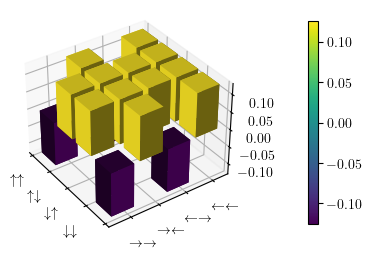
\includegraphics[width=0.6\textwidth]{imgs/wigner-desargues-2-2-s2.png}
      \caption{Función de Wigner del estado
      $\frac{1}{\sqrt{2}}\left(\ket{\uparrow\downarrow} -
      \ket{\downarrow\uparrow}\right)$.}
      \label{fig:wigner-desargues-2-2-s2}
    \end{figure}

    Podemos notar que en la figura
    (\ref{fig:wigner-desargues-2-2-s1}), sumando la función
    de Wigner sobre la primera recta vertical en el espacio
    de fase obtenemos la probabilidad de que el sistema se
    encuentre en el estado $\ket{\uparrow\uparrow}$. Dado
    que el estado es precisamente $\ket{\uparrow\uparrow}$,
    la suma es igual a $1$. En cambio, en la figura
    (\ref{fig:wigner-desargues-2-2-s2}), el estado está en
    una superposición equitativa de los estados
    $\ket{\uparrow\downarrow}$ y $\ket{\downarrow\uparrow}$,
    por lo tanto la probabilidad de observar
    $\ket{\uparrow\downarrow}$ ó $\ket{\downarrow\uparrow}$
    es igual a $\frac{1}{2}$. En cambio, la probabilidad de
    observar el estado $\ket{\uparrow\uparrow}$ ó el estado
    $\ket{\downarrow\downarrow}$ es nula, algo se puede
    observar al sumar la primera y recta vertical
    (respectivamente). Por otro lado, la probabilidad de
    observar el eigenestado asignado a la primera recta
    horizontal
    \[
      \ket \psi
      = \frac{1}{2} \begin{pmatrix} 1\\1\\1\\1 \end{pmatrix},
    \] 
    en el sistema cuántico es
    \[
      |\braket{\psi|\psi_2}|^2
      = \left|\frac{1}{\sqrt{2}}
      \left(\braket{\psi| \uparrow\downarrow} - 
      \braket{\psi| \downarrow\uparrow}\right)
      \right|^2
      = \left|
      \frac{1}{2 \sqrt{2}} - \frac{1}{2 \sqrt{2}}
      \right|^2
      = 0.
    \] 
    Ésto concuerda con la suma de la función de Wigner sobre
    la primera recta horizontal, en donde los puntos se
    anula gracias a la negatividad.

    Por último, grafiquemos un estado `maximalmente
    entrelazado', conocidos como estados GHZ. En la base
    estándar de $\C^2 \otimes \C^2$, se expresa como
    \[
      \ket{GHZ}
      = \frac{1}{\sqrt{2}} \left( \ket{00} + \ket{11}
      \right). 
    \] 
    De acuerdo a la elección de la base del campo, éstos
    estados corresponden a los estados de $\C^{4}$: $\ket{0}$
    y $\ket{\alpha+1}$ respectivamente, los cuales la red
    $Q$ asigna a la primera y última recta vertical del
    espacio de fase discreto:
    \[
      \ket{GHZ}
      = \frac{1}{\sqrt{2}}
      \left( \ket{0} + \ket{\alpha+1} \right). 
    \] 
    La gráfica de la función $W_{\ket{GHZ}}$ se muestra en
    la figura (\ref{fig:wigner-desargues-2-2-ghz}). La
    interpretación es muy similar al estado anterior
    $\ket{\psi_2}$.
    \begin{figure}[ht]
      \centering
      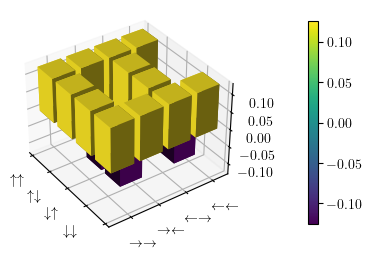
\includegraphics[width=0.6\textwidth]{
      imgs/wigner-desargues-2-2-ghz.png}
      \caption{Función de Wigner del estado $\ket{GHZ}$.}
      \label{fig:wigner-desargues-2-2-ghz}
    \end{figure}
  \end{example}

  En éste capítulo hemos descrito el procedimiento y
  razonamiento de la construcción de la versión de Wootters
  de la función de Wigner, a la que hemos llamado la
  \textit{construcción estándar}. En el siguiente capítulo
  realizamos una definición alternativa de la función de
  Wigner. La metodología permanece igual, pero se utilizan
  conjuntos de bases mutuamente insesgadas que no son
  unitariamente equivalentes a las que se obtienen mediante
  el método de Wootters. La construcción de éstas bases
  difiere en como se \textit{cubre} el espacio de fase
  discreto con \textit{lineas}. Es más general que la
  versión de Wootters en el sentido de que se recupera dicha
  versión cuando las lineas son las rectas en el espacio de
  fase, pero, podemos obtener otras maneras de cubrirlo que
  aun preservan las propiedades geométricas. La idea es
  utilizar éstas estructura geométricas y las MUBs
  alternativas que producen, para formar una función de
  Wigner discreta distinta a la de Wootters.

  \chapter{Construcción no-estándar}

  Para construir la función de Wigner discreta siguiendo la
  metodología de Wootters y Gibbons, es necesario obtener
  al menos un eigenvector mutuo para cada una de las $d+1$
  estrías (recordemos que solo uno es necesario porque la
  propiedad de covarianza bajo traslaciones determina el
  resto). La obtención de los eigenvectores sería
  analíticamente y computacionalmente latoso conforme la
  dimensión va creciendo. Por suerte existen múltiples
  construcciones explícitas de bases mutuamente insesgadas,
  además Godsil y Roy \cite{godsil2009} probaron que las
  construcciones de MUBs más conocidas, debido a Ivánovic,
  Wootters y Fields \cite{wootters1989}, Klappenecker
  \cite{klappenecker2005a} y Bandyophyay
  \cite{bandyopadhyay2001} son todos unitariamente
  equivalentes en el sentido de que existe una
  transformación unitaria que nos lleva de una base a otra.

  Gibbons y Wootters utilizaron los resultados de
  Bandyophyay et al para demostrar que los operadores de
  desplazamiento que corresponden a las traslaciones
  invariantes de una estría son simultáneamente
  diagonalizable. Por otro lado se ha descubierto que las
  MUBs están directamente relacionadas con otros problemas
  en diversas áreas de las matemáticas, como en el algebra
  combinatoria y la matemática discreta. La elección de
  asignar elementos de bases mutuamente insesgadas a rectas
  en el espacio de fase es lo que distingue la construcción
  de Wootters de otros métodos de construcción de funciones
  de Wigner. Como hemos visto, la idea reside en hacer una
  partición del espacio de fase discreto en \textit{rectas}
  paralelas llamadas estrías, pero, la manera en que
  Wootters hace la partición no es la única manera de
  hacerlo. Existen otras formas de separar una malla de $d
  \times d$ en conjuntos de puntos tales que cualesquiera
  dos puntos distintos residen en uno solo de esos
  conjuntos. Éstos objetos han sido estudiados en otras
  áreas de las matemáticas, por ejemplo en la geometría
  finita donde llevan el nombre de \textit{plano afín}
  \cite{kantor2012}. 

  \begin{definition}[Plano afín]
    Un plano afín de orden $d$ es un objeto combinatorio que
    consiste de un conjunto de $d^2$ puntos, junto con
    $d(d+1)$ conjuntos de puntos llamados \textit{lineas},
    tales que cualesquiera dos puntos distintos pasa por una
    única linea. En éste caso las lineas se pueden agrupar
    en $d+1$ clases de lineas `paralelas' de tamaño $d$,
    particionando a todo el conjunto de puntos. 
  \end{definition}

  En su artículo \cite{kantor2012}, Kantor muestra que hay
  una relación íntima entre planos afínes y bases mutuamente
  insesgadas.  Ésto lo hace recordando algunos resultados
  más viejos que conectaban planos afínes con otras
  estructuras algebráicas llamadas \textit{coberturas
  simplécticas} y con familias de subespacios
  unidimiensionales mutuamente ortogonales.  El método de
  construcción de MUBs de Kantor es lo suficientemente
  general para incluir a las construcciones conocidas (en
  particular la de Wootters) y además permite construir MUBs
  que \textit{no} son unitariamente equivalente a las
  construcciones estándares. La idea de éste capítulo es
  utilizar coberturas simplécticas distintas a los de
  Wootters para obtener bases de MUBs no unitariamente
  equivalentes, y por lo tanto una función de Wigner
  distinta que sigue preservando la propiedad tomográfica.
  Unos de los objetivos de éste capítulo es exponer dos
  ejemplos específicos de sistemas cuánticos para los cuales
  podemos construir la función de Wigner no estándar: para
  un sistema de cinco qubits y un sistema de tres qutrits.

  Para construir las MUBs de manera explícita, utilizaremos
  los resultados de Kanat \cite{abdukhalikov2015}, quien nos
  muestra que de \textit{presemicampos simplécticos} es
  posible obtener coberturas simplécticas las cuales a su vez
  nos producen MUBs por medio de los resultados de Kantor,
  éste procedimiento se organiza como en la figura
  (\ref{diag:kanat}). 
  \begin{figure}[h]
    \centering
    \begin{tikzcd}
      \text{Pre-semicampo simpléctico}
      \arrow[d] \\
      \text{Combertura simpléctica}
      %\arrow[d] \\
      %\text{Descomposición ortogonal de $\Sl_n(\C)$}
      \arrow[d] \\
      \text{MUBs completos}
    \end{tikzcd}
    \caption{Metodología resumida de Kanat.}
    \label{diag:kanat}
  \end{figure}
  Kanat expone una relación entre un conjunto completo de
  MUBs y la descomposición ortogonal del álgebra de Lie de
  las matrices $d \times d$ sobre $\C$ de traza nula,
  denotado $\mathfrak{L} = \Sl_d(\C)$, donde el producto de
  Lie está dado por el conmutador de matrices. Una
  descomposición de un álgebra de Lie simple $\mathfrak{L}$
  en una suma directa de subalgebras de Cartan
  \begin{equation}
    \mathfrak{L}
    = \mathfrak{H}_0 \oplus \mathfrak{H}_1 \oplus \cdots
    \oplus \mathfrak{H}_n,
  \end{equation}
  es una descomposición ortogonal si las subálgebras
  $\mathfrak{H}_i$ son ortogonales entre si respecto a la
  forma de Killing en $\mathfrak{L}$.  Las subálgebras de
  Cartán de $\Sl_d(\C)$ consisten de matrices sin traza las
  cuales son diagonales y resulta que están en
  correspondencia con las bases de un conjunto completo de
  MUBs. Kanat cita al siguiente teorema de Boykin et al
  \cite{boykin2005}:
  \begin{theorem}[Boykin et al, Teorema 5.2]
    \label{thm:boykin}
    Los conjuntos maximales de MUBs en $\C^{d}$ están en
    correspondencia con descomposiciones ortogonales del
    álgebra de Lie $\Sl_d(\C)$, donde los subálgebras de
    Cartán de la descomposición son cerrados bajo la
    operación de adjunción.
  \end{theorem}
  La prueba consiste en demostrar que las bases de un
  conjunto completo de MUBs $\mathcal B =
  \{B_0,B_1,\ldots,B_d\}$ están en correspondencia con la
  subálgebra de Cartan $\mathfrak{H}_i$ la cual consiste de
  las matrices sin traza que son diagonales respecto a la
  base $B_i$. De aquí podemos ver la relación con el trabajo
  de Bandyophyay et al y como consecuencia, con la
  construcción estándar de Wootters, ya que la idea
  básicamente se reduce a encontrar una partición de ciertos
  operadores tales que conmuten entre sí. En dicho artículo
  Kanat adicionalmente construye MUBs a partir de
  \textit{funciones planares} y muestra que el grupo de
  automorfismos de un conjunto completo de MUBs es isomorfo
  al grupo de automorfismos de la descomposición ortogonal
  de $\Sl_d(\C)$. No es necesario estudiar la descomposición
  ortogonal de $\Sl_d(\C)$ para construir el conjunto
  completo de MUBs. Basta con construir coberturas
  simplécticas las cuales nos particionan a los operadores
  de Pauli generalizados de tal manera que podemos utilizar
  el teorema de Bandyophyay para garantizar la existencia de
  las MUBs.
  
  Comenzamos por definir a los operadores de desplazamiento
  que actúan sobre el espacio de Hilbert $\H = \C^{d}$ donde
  $d = p^{n}$ para un primo $p$.  Consideremos a un campo
  finito $\mathbb F$ de cardinalidad $d$ como un espacio
  vectorial $V$ unidimensional.  La cardinalidad de $V$ es
  igual a $d$ y etiquetemos a la base estándar de $\C^{d}$
  por los elementos de $V$, es decir, $\{\ket{e_w} : w \in
  V\}$.  Enseguida definamos a los operadores de Pauli
  generalizados, los cuales serán indexados por los
  elementos de $V$.
  \begin{definition}
    Sea $\omega \in \C$ la $p$-ésima raíz primitiva de la
    unidad y sean $u,v \in V$. Definimos a los operadores de
    Pauli generalizados como:
    \begin{align}
      X(u) &: \ket{e_w} \mapsto \ket{e_{w+u}} \\
      Z(v) &: \ket{e_w} \mapsto \omega^{\tr(v w)}
      \ket{e_w}.
    \end{align}
    Además, un operador de desplazamiento arbitrario se
    define como:
    \begin{equation}
      D(u,v) = X(u)Z(v).
    \end{equation}
  \end{definition}
  Las matrices $D(u,v)$ forman una base del espacio de
  matrices complejas de tamaño $d \times d$ de traza nula y
  son los operadores de despalzamiento que también ya
  conocemos.  Además de ésto, las matrices $D(u,v)$ con $u$
  y $v$ distintos del vector cero, generan al algebra de Lie
  $\Sl_n(\C)$. Notemos que ésta definición no está dada por
  potencias de los operadores $X$ y $Z$ ya que ésto solo
  tiene sentido cuando los elementos son los enteros módulo
  $p$. Pero, en caso de que $V = \Z_p$, la definición
  anterior se reduce a nuestra definición del capítulo
  anterior ya que la traza (considerando a $\Z_p$ como una
  extensión de Galois de grado 1) deja invariante a los
  elementos del subcampo. Antes de probar algunas
  propiedades de los operadores de desplazamiento, vamos a
  ligar ésta nueva definición con la de Wootters del capítulo
  anterior.
  \begin{proposition}
    Denotemos a los operadores de desplazamiento que actúan
    sobre un espacio de Hilbert de dimensión prima $p$,
    $\H_p$, por $D_p(a,b)$. Sea $D(u,v) = X(u) Z(v)$ para
    $u, v \in V$, y sea $\varepsilon$ una base del campo. Si
    $\tilde \varepsilon$ es una base dual de $\varepsilon$,
    entonces
    \begin{equation}
      D(u,v)
      = D_p(u_1,\tilde v_1)
      \otimes \cdots \otimes
      D_p(u_n, \tilde v_n),
    \end{equation}
    donde $u_1,\ldots,u_n$ son los componentes de $u$ en la
    base $\varepsilon$ y $\tilde v_1,\ldots,\tilde v_n$ son
    los componentes de $v$ en la base dual, y donde la
    igualdad es en sentido del isomorfismo entre los
    productos tensoriales de $\H_p$ y el espacio $\H$.
  \end{proposition}
  Recordemos que Wootters llegó a la condición de
  conmutatividad de los operadores de Pauli a partir de la
  construcción de la malla cuántica, la cual a su vez estaba
  sujeta a la invarianza de los subespacios (lineas) del
  espacio de fase discreto bajo traslaciones. Ahora deseamos
  identificar la condición necesaria de la conmutatividad
  sin restringirnos (por el momento) por las propiedades de
  la malla cuántica. Primero definimos una forma bilineal
  alternante sobre el espacio vectorial $W = V \oplus V$ de
  dimensión $2n$ sobre el subcampo primo de la extensión de
  Galois. 
  \begin{definition}
    Sea $W = V \oplus V$. Definimos la forma bilineal
    alternante 
    \[
      \langle \cdot, \cdot \rangle : W \to \Z_p
    \]
    para todo $(u,v) \in W$ de la siguiente manera:
    \begin{equation}
      \label{eqn:bilinear_form}
      \langle (u,v), (u',v') \rangle
      = \tr\left( u v' - v u' \right),
    \end{equation}
    donde de nuevo $\tr : \F \to \Z_p$ es la traza de la
    extensión $\GF(p^{n})$ al campo primo. 
  \end{definition}
  Notemos que la forma bilineal es una forma simpléctica.
  Continuemos expresando la acción que tienen los operadores
  de desplazamiento sobre los elementos de la base estándar.
  Por definición tenemos que:
  \begin{align}
    X(u)Z(v) \ket{e_w}
    &= X(u) \omega^{\tr(v w)} \ket{e_w} \\
    &= \omega^{\tr(v \cdot w)} \ket{e_{w+u}}.
  \end{align}
  Por lo tanto
  \begin{align}
    Z(v)X(u) \ket{e_w}
    &= Z(v) \ket{e_{w+u}} \\
    &= \omega^{\tr(v (w+u))} \ket{e_{w+u}} \\
    &= \omega^{\tr(v w) + \tr(v u)}
    \ket{e_{w+u}} \\
    &= \omega^{\tr(v u)} \left( \omega^{\tr(v
    w)} \ket{e_{w+u}} \right) \\
    &= \omega^{\tr(v u)} X(u)Z(v) \ket{e_{w}}.
  \end{align}
  Así que los productos de $X$ y $Z$ satisfacen la relación
  de conmutatividad: $Z(v)X(u) = \omega^{\tr(v \cdot u)}
  X(u)Z(v)$ para todo $u,v \in V$. Utilizando ésto, podemos
  observar que los operadores de desplazamiento satisfacen
  la propiedad de traslación análoga a la de los operadores
  de desplazamiento $D_p(a,b)$:
  \begin{align}
    D(u,v) D(u',v')
    &= X(u)Z(v) X(u')Z(v') \\
    &= X(u) \left( \omega^{\tr(v u')} X(u') Z(v)
    \right) Z(v') \\
    &= \omega^{\tr(v u')} X(u+u') Z(v + v') \\
    &= \omega^{\tr(v u')} D(u+u',v+v')
    \label{eqn:disp_product_relation}.
  \end{align}
  La propiedad de traslación implica la siguiente relación
  de conmutatividad:
  \begin{align}
    D(u',v')D(u,v)
    &= \omega^{\tr(v' u)} D(u'+u,v'+v) \\
    &= \omega^{\tr(u v')} D(u+u',v+v') \\
    &= \omega^{\tr(u v')} \omega^{-\tr(v u')}
    D(u,v)D(u',v') \\
    &= \omega^{\tr(u v' - v u')} D(u,v)D(u',v')
    \\
    &= \omega^{\langle (u,v), (u',v') \rangle}
    D(u,v)D(u',v') \label{eqn:disp_comm_relation}.
  \end{align}
  Usando las propiedades (\ref{eqn:disp_product_relation}) y
  (\ref{eqn:disp_comm_relation}), podemos calcular el
  conmutador de dos operadores de desplazamiento e
  identificar la condición para que el conmutador se anule.
  \begin{proposition}
    Dos operadores de desplazamiento $D(u,v)$ y $D(u',v')$
    conmutan si y solo si la forma simpléctica se anula para
    $(u,v)$ y $(u',v')$, i.e.,
    \begin{equation}
      \label{eqn:disp_comm_condition}
      \langle (u,v), (u',v') \rangle = 0.
    \end{equation}
  \end{proposition}
  \begin{proof}
    Un cálculo directo nos muestra que
    \begin{align}
      [D(u,v),D(u',v')]
      &= D(u,v)D(u',v') - D(u',v')D(u,v) \\
      &= D(u,v)D(u',v') - \omega^{\langle (u,v),(u',v')
      \rangle} D(u,v) D(u',v') \\
      &= \left( 1 - \omega^{\langle (u,v),(u',v') \rangle}
      \right) D(u,v)D(u',v') \\
      &= \omega^{\tr(v \cdot u')} \left( 1 - \omega^{\langle
      (u,v),(u',v') \rangle} \right) D(u+u',v+v').
      \label{eqn:disp_comm}
    \end{align}
  \end{proof}
  Notemos que podemos identificar el espacio de fase
  discreto con el espacio $W = V \oplus V$. La idea de
  Wootters fue identificar subespacios unidimensionales del
  espacio de fase tales que los operadores de desplazamiento
  correspondientes conmutaran. Pero, con la condición
  (\ref{eqn:disp_comm_condition}) podemos identificar
  \textit{más} agrupaciones de los puntos del espacio de
  fase discreto que también anulan la forma simpléctica. A
  las agrupaciones maximales Kantor las llama coberturas
  simplécticas.
  \begin{definition}[Cobertura simpléctica]
    Una cobertura simpléctica $\Sigma$ de un espacio
    simpléctico $W = V \oplus V$ es una familia $\Sigma$ de
    $d+1$ subespacios de $W$ de dimensión $n$ totalmente
    isotrópicos, tales que su intersección uno-a-uno es el
    espacio trivial $0$. 
  \end{definition}
  Un $n$-espacio totalmente isotrópico es un subespacio de
  dimensión $n$ en donde una forma bilineal se anula. En una
  cobertura simpléctica, todo vector de $V \oplus V$ está en
  uno y solo un miembro de $\Sigma$, asi que $\Sigma$
  particiona a los vectores no nulos. Kantor nos dice que
  ésto determina un plano afín de orden $d$, cuyos puntos
  son los vectores en $V \oplus V$ y cuyas lineas son
  traslaciones de los miembros de $\Sigma$ por los elementos
  de $V \oplus V$. Entonces siempre podemos obtener un plano
  afín a partir de una cobertura simpléctica y resulta que
  la partición en lineas rectas de Wootters del espacio de
  fase discreto es precisamente un plano afín, conocido como
  el cobertura de Desargues (ésto lo veremos en los ejemplos
  más adelante).

  Con la construcción anterior de los operadores de
  desplazamiento, y utilizando los resultados de Kantor
  \cite{kantor1996}, Kanat concluye que si $\Sigma = \{W_0,
  W_1, \ldots, W_d\}$ es una cobertura simpléctica, entonces
  existe una descomposición ortogonal del álgebra de Lie
  $\Sl_n(\C)$ donde las subálgebras $\mathfrak{H}_i$ son
  generadas por los operadores de desplazamiento agrupados
  por los puntos del subespacio $W_i$:
  \begin{equation}
    \mathfrak{H}_i = \langle D(u,v) : (u,v) \in W_i \rangle.
  \end{equation}
  De la descomposición ortogonal de $\Sl_d(\C)$ se pueden
  obtener un conjunto de $d+1$ MUBs a partir de la
  diagonalización de los operadores de desplazamiento que
  son generadores de las subálgebras de Cartán
  \cite{boykin2005}, ésto es basicamente lo que Wootters
  hizo mediante los resultados de Bandyophyay. Por suerte,
  Kantor y Kanat nos dan una manera de obtener los MUBs
  \textit{directamente} de la cobertura simpléctica, sin
  necesidad de diagonalizar a los operadores de Pauli.
  
  Por otro lado, es natural pensar que distintas coberturas
  simplécticas nos darán distintos conjuntos de MUBs, pero
  ésto no es el caso en general. De hecho bajo un
  significado particular de equivalencia, muchas de las
  coberturas que parecen ser distintas son iguales. La
  motivación principal de éste trabajo es que para algunas
  dimensiones es posible obtener coberturas simplécticas no
  equivalentes. Kantor demuestró que la inequivalencia de
  coberturas simplécticas conlleva a la inequivalencia de
  MUBs \cite{kantor2012}:
  \begin{theorem}[Kantor (\cite{kantor2012}), Teorema 2.3
    (Inequivalencia)]
    \label{thm:kantor_ineq}
    Toda cobertura simpléctica $\Sigma$ de $V \oplus V$
    determina una conjunto completo de $d+1$ MUBs en
    $\C^{d}$. Además, sea $\Sigma'$ es otra cobertura
    simpléctica de $V \oplus V$, entonces $\Sigma$ y
    $\Sigma'$ son equivalentes bajo una transformación
    lineal de $V \oplus V$ que preserva la forma bilineal
    alternante si y solo si las MUBs respecto a  $\Sigma$ y
    $\Sigma'$ son equivalentes bajo una transformación
    unitaria de $\C^{d}$.
  \end{theorem}

  Como consecuencia del teorema (\ref{thm:kantor_ineq}), si
  logramos encontrar una cobertura simpléctica no
  equivalente, (i.e., encontrar un plano afín no isomorfo al
  de Wootters), obtendremos bases mutuamente insesgadas que
  \textit{no} son unitariamente equivalentes. Podremos
  aplicar el método de construcción de Wootters con éstas
  bases no equivalentes para obtener operadores puntuales
  distintos a los de Wootters y por lo tanto una definición
  alternativa de la función de Wigner discreta, que además,
  por construcción, preserva la propiedad tomográfica
  básica. Para ver ésto, describimos el método que utiliza
  Kanat para obtener las expresiones explicítas de las MUBs,
  y como mencionamos anteriormente, dadas algunas sutilizas
  de los campos de característica par, dividimos la
  descripción en dos casos.
  
  \section{Característica impar}

  De la sección anterior sabemos que un cobertura
  simpléctica nos produce un plano afín y una descomposición
  ortogonal de $\Sl_d(\C)$, la cual a su vez nos brinda un
  conjunto completo de MUBs por medio de la diagonalización
  simultánea de los operadores de desplazamiento
  conmutativos. Existen múltiples construcciones explícitas
  de los eigenvectores de los subconjuntos de $D(\alpha)$,
  iniciando con la construcciones de Ivanovic y Wootters. La
  mayoría son equivalentes y son un caso particular de los
  métodos de Kantor y Kanat. Para nuestro trabajo,
  utilizaremos las construcciones de Kanat y empezamos por
  demostrar el siguiente teorema que nos permitirá expresar
  las MUBs a partir de una cobertura simpléctica. Usaremos
  la forma simpléctica (\ref{eqn:bilinear_form}) y
  consideramos a $V$ como el espacio unidimensional sobre la
  extensión de Galois, i.e., $V = \F = \GF(p^{n})$ donde en
  ésta sección, $p$ es un número primo impar.  Recordemos
  que $\{\ket{e_w} : w \in V\}$ es la base estándar de
  $\C^{p^{n}}$ etiquetada por los elementos de la extensión
  de Galois.

  \begin{theorem}
    \label{thm:h_mubs}
    Sea $\Sigma$ una cobertura simpléctica de $W = V \oplus
    V$ y sea $h : V \to V$ un mapeo lineal tal que
    \begin{equation}
      \{(u,h(u)) : u \in V\} \in \Sigma.
    \end{equation}
    Entonces para todo $v \in V$, el vector dado por
    \begin{equation}
      \ket{b_{h,v}}
      = \sum_{w \in V}^{}
      \omega^{\tr\left(
          \frac{1}{2} w
        h(w) + v w
      \right) } \ket{e_w}
    \end{equation} 
    es un eigenvector del operador de desplazamiento
    $D(u,h(u))$ para todo $u \in V$.
  \end{theorem}
  \begin{proof}
    Calculando directamente obtenemos:
    \begin{align}
      D(u,h(u)) \ket{b_{h,v}}
      &= \sum_{w \in V}^{}
      \omega^{\tr\left(
          \frac{1}{2} w h(w) + v w
      \right) }
      X(u)Z(h(u)) \ket{e_w} \\
      &= \sum_{w \in V}^{}
      \omega^{\tr\left(
          \frac{1}{2} w h(w) + v w
      \right) }
      \omega^{\tr(h(u) w)}
      \ket{e_{w+u}} \\
      &= \sum_{w \in V}^{}
      \omega^{\tr\left(
          \frac{1}{2} w h(w) + v w + h(u) w
      \right) }
      \ket{e_{w+u}} \\
      &= \sum_{w \in V}^{}
      \omega^{\tr\left(
          \frac{1}{2} (w-u) h(w-u) + v (w-u) + h(u) (w-u)
      \right) }
      \ket{e_w} \\
      &= \sum_{w \in V}^{}
      \omega^{\tr\left(
        \frac{1}{2}(w-u) h(w) + \frac{1}{2}(w-u) h(u)
        + v w - v u + h(u) w - h(u) u
      \right) }
      \ket{e_w}.
      \label{eqn:trace_eig}
    \end{align}
    La traza en la ecuación (\ref{eqn:trace_eig}) se puede
    expresar como
    \begin{equation}
      \tr\left(
        \frac{1}{2} w h(w) + v w
      \right)
      + \frac{1}{2}\tr\left(
        h(u) w - u h(w)
      \right)
      - \tr\left(
        \frac{1}{2} u h(u) + v u
      \right),
    \end{equation}
    pero por hipótesis $(u,h(u))$ pertenece a algún $W_i \in
    \Sigma$, por lo tanto
    \begin{align}
      \tr\left( u h(w) - h(u) w \right)
      = \langle (u,h(u)), (w,h(w)) \rangle
      = 0,
    \end{align}
    ya que todo $W_i$ es totalmente isotrópico respecto a la
    forma bilineal alternante. Así que el exponente de
    $\omega$ en (\ref{eqn:trace_eig}) está dado por: 
    \begin{equation}
      \tr\left( \frac{1}{2} w h(w) + v w \right)
      - \tr\left( \frac{1}{2} u h(u) + v u \right).
    \end{equation}
    Con ésto retomamos el cálculo inicial y verificamos que
    $\ket{b_{h,v}}$ efectivamente es un eigenvector de
    $D(u,h(u))$:
    \begin{align}
      D(u,h(u)) \ket{b_{h,v}}
      &= \sum_{w \in V}^{}
      \omega^{\tr\left(
          \frac{1}{2} w h(w) + v w
      \right)
      - \tr\left(
        \frac{1}{2} u h(u) + v u
      \right) } \ket{e_w} \\
      &= \omega^{-\tr\left(
          \frac{1}{2} u h(u) + v u
      \right) }
      \sum_{w \in V}^{}
      \omega^{\tr\left(
        \frac{1}{2} w h(w) + v w
      \right) } \ket{e_w} \\
      &= \omega^{-\tr\left(
        \frac{1}{2} u h(u) + v u
      \right) } \ket{b_{h,v}}.
    \end{align}
  \end{proof}
  \begin{corollary}
    Los vectores $\ket{b_{h,v}}$ del teorema
    \ref{thm:h_mubs} son mutuamente insesgados.
  \end{corollary}
  \begin{proof}
    Dado que $\Sigma$ es una cobertura simpléctica, los
    subespacios $W_h = \{(u, h(u) : u \in \F\} \in \Sigma$,
    son totalmente isotrópicos. Por lo tanto los conjuntos
    de operadores
    \[
      \{D(u,h(u)) : u \in \F\}, 
    \] 
    son conjuntos maximales de operadores de Pauli
    conmutativos. Se sigue del teorema \ref{thm:bandy}
    (Bandyophyay et al) que los conjuntos de eigenvectores
    simultáneos correspondientes a cada subespacio $W_h$ son
    mutuamente insesgados.
    %Un cálculo directo nos brinda lo siguiente. Sean $h$ y
    %$h'$ mapeos lineales tales que
    %\[
    %  W_h
    %  = \{(u,h(u)) : u \in V\},
    %  \quad \text{y} \quad
    %  W_{h'}
    %  = \{(u,h'(u)) : u \in V\}
    %\] 
    %son elementos distintos de la cobertura simpléctica
    %$\Sigma$.  Entonces
    %\begin{align}
    %  \braket{b_{h,v}|b_{h',v'}}
    %  &= \sum_{w \in V}^{} 
    %  \omega^{-\tr\left( \frac{1}{2} w h(w) + vw \right) }
    %  \omega^{\tr\left( \frac{1}{2} w h'(w) + v'w \right) } \\
    %  &= \sum_{w \in V}^{}
    %  \omega^{\tr\left( \frac{1}{2} w (h'(w) - h(w)) + w(v'
    %  - v) \right) }.
    %\end{align}
    %Primero supongamos que $h = h'$. Si $v = v'$ entonces
    %$\braket{b_{h,v}|b_{h',v'}} = d$. Si $v \neq v'$,
    %entonces
    %\begin{equation}
    %  \braket{b_{h,v}|b_{h',v'}}
    %  = \sum_{w \in V}^{} \omega^{\tr\left( w(v'-v) \right) }
    %  = \sum_{z \in V}^{} \omega^{\tr(z)}
    %  = 0,
    %\end{equation}
    %donde la última suma se anula porque $\sum_{j = 0}^{p-1}
    %\omega^{j} = 0$ (ver sección de caracteres aditivos del
    %apéndice \ref{sec:fields}). Ésto prueba que
    %los vectores de la misma base son ortonormales. Ahora
    %supongamos que $h \neq h'$, entonces PENDIENTE.
  \end{proof}
  El teorema anterior nos permite diagonalizar de manera
  simultánea a los operadores de desplazamiento que conmutan
  entre si para una cobertura simpléctica dada.  La cuestión
  natural ahora es, ¿cómo obtener coberturas simplécticas?, y
  sobre todo, ¿cómo obtener coberturas que no son equivalentes?
  Kantor comenta que encontrar coberturas simplécticas no es
  trivial, pero podemos construir algunas por medio de
  presemicampos y semicampos.\footnote{Existen coberturas
    simplécticas que no provienen de un semicampo
    simpléctico, pero para nuestra construcción alternativa
  basta utilizar aquellos que sí provienen de semicampos.}.
  Introducimos brevemente algunas nociones que vinculan los
  presemicampos y las coberturas simplécticas, pero no
  seremos muy rigurosos ya que para éste trabajo nos basta
  con tomar los ejemplos dados por Kantor \cite{kantor2012}
  para construir nuestras coberturas no equivalentes.
  \begin{definition}[Presemicampo y semicampo]
    \label{def:presemifield}
    Un presemicampo es un anillo sin divisores del cero, y
    con solo la propiedad distributiva (derecha e
    izquierda). Un semicampo es un presemicampo con una
    identidad multiplicativa.
  \end{definition}
  A partir de un campo finito $\F$ podemos obtener un
  presemicampo finito al introducir una operación nueva
  $\circ : \F \times \F \to \F$. La operación de suma es la
  del campo finito, por lo tanto la definición
  (\ref{def:presemifield}) nos dice que el semicampo finito
  es el conjunto $\F$ tal que
  \begin{enumerate}
    \item $\F$ es un grupo abeliano bajo la suma, con
      identidad $0$.
    \item Si $x \circ y = 0$, entonces $x = 0$ ó $y = 0$.
    \item Satisface las propiedades distributivas
      \[
        x \circ (y + z) = x \circ y + x \circ z,
        \quad
        (x + y) \circ z = x \circ z + y \circ z.
      \] 
  \end{enumerate}
  Notemos que todo campo finito es un semicampo y un
  presemicampo. Kantor comenta que todo presemicampo
  determina un cobertura $\Sigma$ del espacio $V \oplus V$
  por medio de la multiplicación. Ésta cobertura consiste de
  los subespacios
  \begin{equation}
    \label{eqn:presemi_spread}
    \{(0,v) : v \in \mathbb F\},
    \quad 
    \{(u, u \circ m) : u \in \mathbb F\}
    \quad
    \text{para todo } m \in \mathbb F.
  \end{equation}
  Decimos que un presemicampo es \textit{simpléctico} si la
  cobertura que genera es simpléctica respecto a
  algúna forma bilineal alternante. Entonces dado un
  presemicampo simpléctico podemos generar el conjunto
  completo de MUBs simplemente utilizando la operación del
  presemicampo.

  \begin{theorem}[Kanat (\cite{abdukhalikov2015}) Teorema 3.3]
    \label{thm:kanat_presemi_mubs}
    Sea $F = \GF(p^{n})$. Si $(F, +, \circ)$ es un
    presemicampo simpléctico finito de característica impar,
    entonces los conjuntos
    \begin{equation}
      B_\infty = \{\ket{e_w} : w \in F\},
      \quad
      B_m = \{\ket{b_{m,v}} : v \in F\}
    \end{equation}
    donde 
    \begin{equation}
      \label{eqn:kanat_presemi_mubs}
      \ket{b_{m,v}}
      = \frac{1}{\sqrt{d}} \sum_{w \in F}^{}
      \omega^{\tr\left(
          \frac{1}{2} w (w \circ m) + v w
      \right) } \ket{e_w},
    \end{equation} 
    para todo $m \in F$ forman un conjunto completo de MUBs.
  \end{theorem}
  \begin{proof}
    Si la cobertura que genera la operación del presemicampo
    es una cobertura simpléctica, entonces el teorema
    \ref{thm:h_mubs} nos permite construir el conjunto
    completo de MUBs donde el mapeo $h : V \to V$ está dado
    por la operación $\circ$ del presemicampo. La linealidad
    de $h$ se sigue de la distributividad de la operación
    del presemicampo.
  \end{proof}

  Para poder utilizar utilizar el teorema
  \ref{thm:kanat_presemi_mubs}, debemos formar un
  presemicampo simpléctico. Dado que todo presemicampo forma
  una cobertura $\Sigma$, solo hemos trasladado la
  dificultad de encontrar una cobertura simpléctica a la
  busqueda de presemicampos cuya cobertura es simpléctica,
  i.e., una cobertura de $d+1$ subespacios totalmente
  isotrópicos. Por suerte, en \cite{kantor1982} Kantor
  genera múltiples coberturas simplécticas a partir de
  presemicampos y en lo que sigue del trabajo hemos elegido
  algunos de ellos para poder construir MUBs no
  equivalentes. El ejemplo más sencillo es el que está dado
  simplemente por la multiplicación del campo finito.
  \begin{definition}[Cobertura Desarguesiana]
    \label{def:desarguesian_semifield}
    Sea $\F = \GF(p^{n})$ un campo finito. En particular
    $\F$ es un presemicampo con la operación
    \begin{equation}
      w \circ m = w m.
    \end{equation}
    La cobertura simpléctica generada por éste presemicampo
    se conoce como el cobertura Desarguesiana y consiste
    simplemente de los subespacios unidimensionales de $V
    \oplus V$ sobre $\F$.
  \end{definition}
  Las MUBs que Godsil y Roy probaron que son unitariamente
  equivalentes a las mubs `estándares', incluyendo a la de
  Wooters, son casos específico de MUBs generados por una
  cobertura Desarguesiana. Por lo tanto utilizando la
  definición \ref{def:desarguesian_semifield} y el teorema
  \ref{thm:kanat_presemi_mubs} podemos construir las bases
  mutuamente insesgadas de Wootters. En éste caso la
  cobertura simpléctica $\Sigma$ está dada por los
  subespacios
  \begin{equation}
    0 \oplus V
    \quad \text{ y } \quad
    \{(u,mu) : u \in V\},
    \quad m \in V,
  \end{equation}
  y el plano afín correspondiente está determinado por las
  rectas:
  \begin{equation}
    x = 0
    \quad
    y = mx,
    \quad
    x \in \GF(p^{n}),
  \end{equation}
  las cuales reconocemos como los rayos de Wootters. Se
  sigue que para todo $v \in V$, el vector
  \begin{equation}
    \label{eqn:desargues_vectors}
    \ket{b_{m,v}}
    = \sum_{w \in V}^{} \omega^{\tr\left( \frac{1}{2} m w^2
    + v m\right) } \ket{e_w},
  \end{equation} 
  es un eigenvector simultáneo de los operadores de
  desplazamiento $D(u,mu)$ con $u \in \GF(p^{n})$. En éste
  caso el número $m \in \GF(p^{n})$ identifica la pendiente
  del rayo y por lo tanto identifica a una de las estrías de
  Wootters.

  En vista del teorema de no-equivalencia de Kantor, dado
  una cobertura simpléctica no equivalente a la
  Desarguesiana, podremos obtener un conjunto de MUBs no
  equivalentes a las de Wootters. Para característica impar
  el siguiente presemicampo genera una cobertura simpléctica
  no equivalente a la Desarguesiana \cite{kantor1982}.
  \begin{definition}[Campo torcido de Albert]
    \label{def:alberts_spread}
    Sea $n$ impar y sea $s \in \N$ un primo relativo de $n$
    tal que $1 \leq s \leq \frac{n}{2}$ y consideremos el
    campo finito $\GF(p^{n})$. La operación
    \begin{equation}
      w \circ m
      = mw^{p^{n-s}} + m^{p^{s}} w^{p^{s}},
      \quad m \in \GF(p^{n}),
    \end{equation}
    brinda a $\GF(p^{n})$ una estructura de presemicampo,
    conocido como el campo torcido de Albert.
  \end{definition}
  Kantor muestra que éste presemicampo genera una cobertura
  simpléctica $\Sigma$ de $V \oplus V$ que no es equivalente
  a la Desarguesiana. Utilizando el teorema
  \ref{thm:kanat_presemi_mubs} obtenemos el sguiente
  conjunto completo de MUBs:
  \begin{align}
    \ket{b_{m,v}}
    &= \sum_{w \in V}^{}
    \omega^{\tr\left(
      \frac{1}{2} w (w \circ m) + a w
    \right) } \\
    &= \sum_{w \in V}^{}
    \omega^{\tr\left(
      \frac{1}{2}
      \left(
        mw^{p^{n-s}+1} + m^{p^{s}}w^{p^{s}+1}
      \right) + v w
    \right) } \ket{e_w},
  \end{align}
  donde $m, v \in V$. Por el teorema \ref{thm:kantor_ineq},
  éstas MUBs no son unitariamente equivalentes a las MUBs
  generadas por la ecuación (\ref{eqn:desargues_vectors}).
  Notemos que el espacio de Hilbert de dimensión $3^{3} =
  27$ es el espacio de dimensión más pequeña para el cual
  podemos construir éste conjunto de MUBs en particular. Más
  adelante lo utilizaremos para construir y comparar dos
  funciones de Wigner para sistemas de tres qutrits.
    
  \section{Característica par}

  Para obtener expresiones explícitas de un conjunto
  completo de bases mutuamente insesgadas para el espacio de
  Hilbert $\C^{d}$ con $d = 2^{n}$, es necesario hacer
  modificaciones al procedimiento anterior. La metodología
  permanece igual, dado un presemicampo simpléctico
  obtenemos una cobertura simpléctica y podemos construir
  las MUBs de manera explícita con la operación del
  presemicampo, solo que la expresión de los eigenvectores
  de los operadores de desplazamiento involucra operaciones
  que no solo suceden en el campo finito si no en un
  \textit{anillo de Galois}.  Una idea intuitiva de porque
  la construcción impar no funciona en éste caso se debe a
  la necesidad de utilizar una raíz primitiva compleja en
  las expresiones de los vectores. Por lo tanto es necesario
  utilizar la cuarta raíz primitiva para evitar fases de
  solo $-1$ ó $1$. Los detalles técnicos son más
  involucrados, pero se pueden encontrar en el artículo
  sobre códigos de Kerdock sobre $\Z_4$ y coberturas
  simplécticas escrito por Kantor et al \cite{kantor1982}.

  Sea $\F = \GF(2^{n})$ el campo de Galois y $\omega \in \C$
  una cuarta raíz primitiva de la unidad. Sea $R =
  \GR(4^{n})$ el anillo de Galois de característica cuatro
  (ver apéndice \ref{sec:fields} para un resumen de
  extensiones de anillos). Existe un elemento $\xi$ de orden
  $2^{n}-1$ el cual es una raiz de un único polinomio
  primitivo mónico $h(x)$ de grado $n$ sobre $\Z_4$ que
  además divide a $x^{2^{n}-1} - 1$ en $\Z_4[x]$, por lo que
  es una $2^{n}-1$-ésima raíz primitiva de la unidad en el
  anillo de Galois. El conjunto \textit{Teichmüller} $T
  \subset R$, está dado por potencias de éste elemento,
  \begin{equation}
    T = \{0,1,\xi,\xi^2,\ldots,\xi^{2^{n}-2}\},
  \end{equation}
  y sin el $0$ es subgrupo multiplicativo de tamaño $2^{n}$
  que es isomorfo a $\F$. En ocasiones el generador del
  anillo coincide con la raíz $\xi$, pero ésto no es el caso
  general. Todo elemento $x \in R$ puede ser expresado como
  la combinación lineal de elementos $a,b$ del Teichmüller
  en la forma $x = a + 2b$.  Utilizando ésta expresión
  multiplicativa ó $2$-ádica de $x$, la traza del anillo de
  Galois, $\tr : R \to \Z_4$ se define como
  \begin{equation}
    \tr(x)
    = \left(a + a^2 + \cdots + a^{2^{n-1}}\right) + 2\left(
    b + b^2 + \cdots + b^{2^{n-1}}\right).
  \end{equation}
  La traza es lineal respecto a la suma para todos los
  elementos de $R$. Por otro lado, el cociente $R / 2R$ es
  isomorfo al anillo de Galois $\GF(2^{n})$, así que para
  todo elemento $u \in \GF(2^{n})$ existe un único elemento
  $\hat u \in T$, el cual Kanat nombra como el \textit{lift}
  de $u$ al Teichmüller. 

  Con lo anterior podemos enunciar el teorema equivalente a
  \ref{thm:kanat_presemi_mubs} para el caso de campos de
  característica par:
  \begin{theorem}
    \label{thm:kanat_even}
    Sea $V = \GF(2^{n})$ con la operación $\circ$ un
    presemicampo simpléctico. Entonces la base éstandar
    $B_\infty = \{\ket{e_w} : w \in V\}$ junto con los
    conjuntos $B_m = \{\ket{b_{m,v}} : v \in V\}$ cuyos
    elementos están dados por
    \begin{equation}
      \ket{b_{m,v}}
      = \frac{1}{\sqrt{d}} \sum_{w \in V}^{}
      \omega^{\tr\left(
        \hat w ( \hat w \circ \hat m ) + 2 \hat w \hat v
      \right) } \ket{e_w},
    \end{equation}
    forman un conjunto maximal de $2^{n} + 1$ bases
    mutuamente insesgadas.
  \end{theorem}
  \begin{proof}
    La demostración es muy similar a la del teorema
    \ref{thm:kanat_presemi_mubs}, solo con algunos detalles
    causados por el lift al Teichmüller. En particular,
    Kanat extiende la operación del presemicampo al conjunto
    $T \times T$ de la siguiente manera. Si $x, y \in F$,
    entonces la operación del presemicampo se puede expresar
    como
    \[
      x \circ y
      = \sum_{i,j}^{} a_{ij} x^{2^{i}} y^{2^{j}}.
    \] 
    Luego se extiende el producto $\circ$ a $T \times T$
    como
    \[
      \hat x \circ \hat y
      = \sum_{i,j}^{} \widehat{a_{ij}} \hat{x}^{2^{i}}
      \hat{y}^{2^{j}}. 
    \] 
    Con ésto se puede demostrar que dado un presemicampo
    simpléctico, los vectores del teorema
    \ref{thm:kanat_even} son precisamente los eigenvectores
    de los operadores de desplazamiento $D(u,u\circ m)$ para
    todo $u \in V$.  Se pueden consultar los detalles en
    \cite{abdukhalikov2015}.
    %Demostraremos que para todo $m,v \in \GF(2^{n})$ el
    %vector $\ket{d_{m,v}}$ es un eigenvector de los
    %opeardores $D(u,u\circ m)$ para todo $u \in V$.
    %\begin{align}
    %  D(u,u\circ m) \ket{d_{m,v}}
    %  &= \sum_{w \in \GF(2^{n})}^{}
    %  \omega^{\tr\left(
    %      \hat w \cdot (\hat w \circ \hat m)
    %      + 2 \hat w \hat v
    %      + 2 \hat w \cdot \widehat{u \circ m}
    %  \right)}
    %  \ket{e_{w+u}} \\
    %  &= \sum_{w \in \GF(2^{n})}^{}
    %  \omega^{\tr\left(
    %    (\widehat{w+u}) \cdot ((\widehat{w+u}) \circ \hat m) + 2
    %    (\widehat{w+u}) \hat v + 2 (\widehat{w + u}) \cdot
    %    \widehat{u \circ m}
    %  \right)}
    %  \ket{e_w}
    %\end{align}
    %Ahora, si $w,u,v \in \GF(2^{n})$ son tales que $w = u +
    %v$, entonces
    %\[
    %  \hat w = \hat u + \hat v + 2 \sqrt{\hat u \hat v}.
    %\]
    %Por lo tanto $\widehat{w+u} = \hat w + \hat u + 2
    %\sqrt{\hat w \hat u}$. Por el momento solo consideremos
    %la expresión dentro de la traza en la ecuación ().
    %Haciendo la sustitución correspondiente y expandiendo
    %términos obtenemos
    %\begin{align}
    %  &(\hat w + \hat u + 2 \sqrt{\hat w \hat u}) \cdot
    %    ((\hat w + \hat u + 2 \sqrt{\hat w \hat u}) \circ
    %    \hat m) + 2(\hat w + \hat u) \hat v + 2(\hat w +
    %    \hat u) \cdot (\hat u \circ \hat m)) \\
    %  &= \hat w \cdot (\hat w \circ \hat m) + \hat w \cdot
    %  (\hat u \circ \hat m) + \hat w \cdot (2\sqrt{\hat w
    %  \hat u} \circ \hat m) + 
    %\end{align}
  \end{proof}
  
  De nuevo podemos construir una cobertura Desarguesiana
  mediante la operación del campo finito. Recordemos que
  ésto significa que $x \circ y = xy$. El conjunto $\Sigma$
  de espacios uni-dimensionales sobre $\GF(2^{n})$ de $W = V
  \oplus V$ es una cobertura simpléctica de $W$.  De nuevo
  ésto nos brinda el plano afín
  \[
    x = 0
    \quad \text{ y } \quad
    y = mx,
  \]
  para todo $m \in F$, los cuales reconocemos como los rayos
  de las estrías de Wootters. Para formar un conjunto de
  MUBs no equivalentes al de Wootters, utilizamos otra
  cobertura simpléctica que nos brinda Kantor.
  \begin{definition}
    \label{def:kantor_even_alt}
    Sea $\F = \GF(2^{n})$. Supongamos que $n >
    3$ e impar. Entonces el campo finito con la operación
    \begin{equation}
      x \circ m
      = m^2x + m\tr(x) + \tr(mx),
    \end{equation}
    es un presemicampo simpléctico.
  \end{definition}
  Kantor prueba que la cobertura simpléctica de $V \oplus V$
  generada por éste presemicampo no es equivalente al
  Desarguesiana \cite{kantor2012}. Con el teorema
  \ref{thm:kanat_even} podemos obtener una expresión
  explícita de las MUBs haciendo las operaciones pertinentes
  en el anillo de Galois.

  \section{Función de Wigner discreta no estándar}

  Vamos a recapitular la sección anterior. Dado un campo
  finito $\F$ siempre podemos formar un presemicampo
  mediante una nueva operación $\circ$. Todo presemicampo
  genera una cobertura $\Sigma$ del espacio $V \oplus V$
  donde $V = \F$, que consiste de los subespacios
  \[
    0 \oplus V,
    \quad
    \text{y}
    \quad
    \{(w, w \circ m) : w \in V\} 
    \quad \text{para todo } m \in \F.
  \] 
  En ocasiones, la cobertura formada por la operación del
  semicampo será totalmente istrópico respecto a una forma
  bilineal alternante. En particular nos interesa los
  presemicampos que generan coberturas que son simplécticas
  respecto a la forma definida en (\ref{eqn:bilinear_form}).
  Los elementos de un subespacio de la cobertura simpléctica
  por definición anulan a la forma bilineal alternante, ésto
  a su vez es una condición necesaria para que dos
  operadores de desplazamiento conmuten, si son los
  operadores correspondientes a puntos de los subconjuntos
  de la cobertura.  Dado que los operadores de
  desplazamiento son diagonalizables, dos operadores
  conmutativos nos brindan una base de eigenvectores del
  espacio de Hilbert simultánea. Además como la cobertura
  simpléctica es maximal, obtenemos una partición de los
  operadores de desplazamiento en subconjuntos de operadores
  conmutativos, y obtenemos un conjunto maximal de bases
  mutuamente insesgadas gracias a las construcciones de la
  sección anterior.

  Utilizando nuestra notación, ésto significa que los
  vectores $\ket{b_{m,v}}$ para todo $v \in \F$ corresponden
  a las \textit{curvas} $\{(u, u \circ m) : u \in \F\}$ y a
  sus traslaciones; además son eigenvectores de los
  operadores $D(u, u \circ m)$ para todo $u \in \F$. Cada
  base de eigenvectores es invariante bajo el grupo de
  Pauli \cite{calderbank}, ésto significa que al operar un
  eigenestado por un operador de desplazamiento, obtendremos
  algún otro eigenestado correspondiente a la misma base (o
  al mismo eigenestado si el operador corresponde a las
  traslaciones que dejan invariante a las curvas de la
  estría). Por lo tanto, despues de asignar un eigenestado
  al rayo, el resto de las asignaciones de eigenestados
  quedan determinados por desplazamientos.

  Ésto es precisamente lo que Wootters formó en su
  construcción de la función de Wigner discreta. Sus rectas
  corresponden a las lineas del plano afín, cada punto de la
  linea deja invariante a la linea bajo traslaciones en el
  espacio de fase discreto, por lo tanto el estado cuántico
  asignado a la recta debe corresponder a un eigenvector de
  los operadores de desplazamiento con puntos en en esa
  linea. Vamos a construir los operadores puntuales de la
  misma manera, donde las rectas de Wootters son
  reemplazadas por las curvas de la cobertura simpléctica en
  cuestión. El caso de la cobertura Desarguesiana coincide
  con las rectas de Wootters.
  \begin{definition}
    Sea $\rho$ un operador de densidad. La función de Wigner
    no estándar, denotada como $W_\rho^{\mathcal K}$ en
    referencia a Kantor, se define como
    \begin{equation}
      W_\rho^{\mathcal K}
      = \Tr\left( \rho A^{\mathcal K}(\alpha) \right),
    \end{equation}
    donde los operadores puntuales son
    \begin{equation}
      A^{\mathcal K}(\alpha)
      = \sum_{\alpha \ni \lambda}^{} Q(\lambda) - I,
    \end{equation}
    para toda curva $\lambda$ de la cobertura que contienen
    al punto $\alpha$.
  \end{definition}
  Elegimos la convención de tomar el primer elemento de las
  bases generadas de manera algorítmica por los teoremas
  \ref{thm:kanat_presemi_mubs} y \ref{thm:kanat_even}
  respectivamente como el estado correspondiente al rayo.
  Los estados posteriores de cada estría quedan determinados
  por los operadores de desplazamiento correspondientes.

  \begin{proposition}
    Los operadores puntuales $A^{\mathcal K}(\alpha)$ donde
    $\alpha = (a,b) \in \F \oplus \F$ satisfacen las
    siguientes propiedades
    \begin{enumerate}
      \item Son auto-adjuntos.
      \item Son de traza unitaria.
      \item Son ortogonales bajo el producto interno de
        Hilbert-Schmidt.
    \end{enumerate}
  \end{proposition}
  \begin{proof}
    Las pruebas para cada punto son practicamente iguales a
    las pruebas de la proposición (\ref{prop:point_props}).
    Que los operadores puntuales sean auto-adjuntos y de
    traza unitaria es consecuencia de que los operadores
    $Q(\lambda)$ que constituyen al operador puntual son
    auto-adjuntos y de traza unitaria. La prueba del tercer
    punto solo dependía de que las bases fuera mutuamente
    insesgadas, y de la estructura geométrica del espacio de
    fase discreto. En particular, sabemos que la cobertura
    simpléctica genera un plano afín, el cual preserva la
    propiedad de que por cada punto pasan $d+1$ curvas y que
    las curvas paralelas no se intersectan, por lo tanto
    podemos utilizar el mismo argumento de conteo.
  \end{proof}
  Como consecuencia de la proposición anterior, la
  construcción no estándar también satisface las propiedades
  deseadas de una función de Wigner.
  \begin{proposition}
    Sea $\rho$ un estado cuántico y $W_\rho^{\mathcal K}$ su
    función de Wigner discreta no estándar. Entonces
    \begin{enumerate}
      \item $W_\rho^{\mathcal K}$ es real.
      \item La suma de $W_\rho^{\mathcal K}$ sobre cualquier
        curva $\lambda$ del plano afín es igual al valor
        esperado de $Q(\lambda)$ en el estado $\rho$.
      \item La suma de $W_\rho^{\mathcal K}$ sobre todo el
        espacio de fase discreto es igual a $1$.
      \item La función de Wigner no estándar es covariante
        bajo traslaciones en el espacio de fase discreto.
    \end{enumerate}
  \end{proposition}
  \begin{proof}
    De nuevo la demostración es prácticamente idéntica a la
    de la construcción estándar. Los primeros tres puntos
    surgen directamente de las propiedades de los operadores
    puntuales. La cuarta propiedad depende del hecho de que
    $Q$ sea covariante bajo traslaciones, pero ésto también
    se satisface ya que el grupo de Pauli deja invariante
    (salvo permutaciones) a cada base ortonormal de las MUBs
    producidas por cualquier cobertura simpléctica.
  \end{proof}

  \section{Ejemplos}

  El primer ejemplo de ésta sección consiste en calcular las
  bases mutuamente insesgadas para el sistema cuántico de un
  par de qubits. Utilizaremos el teorema
  \ref{thm:kanat_even} para la construcción notando que las
  bases obtenidas son equivalentes a las de Wootters (salvo
  permutaciones).  Despues, daremos dos ejemplos para los
  cuales calcularemos dos conjuntos completos de MUBs: un
  conjunto estándar (cobertura Desarguesiana) y un conjunto
  no estándar. En la siguiente sección utilizaremos ambos
  conjuntos para comparar las funciones de Wigner.

  \begin{example}
    Consideremos el sistema cuántico de dos qubits. El
    espacio de Hilbert es $\H = \C^2 \otimes \C^2 \cong
    \C^{4}$. 
  \end{example}
  El espacio de fase discreto será una malla de
  $4 \times 4$ pares cuyos componentes son elementos del
  campo finito $\GF(2^2)$. El anillo de Galois
  correspondiente será $\GR(4^{2})$, para construirlo
  consideramos el polinomio $f(x) = x^2+x+1 \in \Z_4[x]$
  para formar el cociente
  \[
    \GR(4^2) \cong \Z_4[x] / \langle x^2+x+1 \rangle.
  \] 
  En éste caso la raíz del polinomio $f(x)$ es una
  $2^{2}-1$-ésima raíz de la unidad del anillo de Galois.
  Por definición el conjunto Teichmüller está dado por $T =
  \{0,1,\xi,\xi^2\}$, y la traza se cálcula como
  \[
    \tr(x) = (a + a^2) + 2(b + b^2),
  \] 
  donde $a + 2b$ es la representación $2$-ádica de $x$.
  Vamos a utilizar el cobertura Desarguesiana para éste
  primer ejemplo por lo tanto la operación del presemicampo
  es simplemente el producto en el campo finito, $x \circ y
  = xy$. La cobertura simpléctica consiste de los
  subespacios de $V \oplus V$ dados por $0 \oplus V$, $\{(u,
  mu) : u \in \GF(2^2)\}$ para todo $m \in \GF(2^2)$.  Los
  rayos del plano afín son las rectas
  \[
    x = 0,
    \quad
    y = mx, \quad m \in \GF(2^2),
  \] 
  y se muestran en la figura (\ref{fig:2-2-desargues-plane}).
  \begin{figure}[ht]
    \centering
    \scalebox{0.8}{
      %% Creator: Matplotlib, PGF backend
%%
%% To include the figure in your LaTeX document, write
%%   \input{<filename>.pgf}
%%
%% Make sure the required packages are loaded in your preamble
%%   \usepackage{pgf}
%%
%% Also ensure that all the required font packages are loaded; for instance,
%% the lmodern package is sometimes necessary when using math font.
%%   \usepackage{lmodern}
%%
%% Figures using additional raster images can only be included by \input if
%% they are in the same directory as the main LaTeX file. For loading figures
%% from other directories you can use the `import` package
%%   \usepackage{import}
%%
%% and then include the figures with
%%   \import{<path to file>}{<filename>.pgf}
%%
%% Matplotlib used the following preamble
%%   
%%   \makeatletter\@ifpackageloaded{underscore}{}{\usepackage[strings]{underscore}}\makeatother
%%
\begingroup%
\makeatletter%
\begin{pgfpicture}%
\pgfpathrectangle{\pgfpointorigin}{\pgfqpoint{3.500000in}{3.500000in}}%
\pgfusepath{use as bounding box, clip}%
\begin{pgfscope}%
\pgfsetbuttcap%
\pgfsetmiterjoin%
\definecolor{currentfill}{rgb}{1.000000,1.000000,1.000000}%
\pgfsetfillcolor{currentfill}%
\pgfsetlinewidth{0.000000pt}%
\definecolor{currentstroke}{rgb}{1.000000,1.000000,1.000000}%
\pgfsetstrokecolor{currentstroke}%
\pgfsetdash{}{0pt}%
\pgfpathmoveto{\pgfqpoint{0.000000in}{0.000000in}}%
\pgfpathlineto{\pgfqpoint{3.500000in}{0.000000in}}%
\pgfpathlineto{\pgfqpoint{3.500000in}{3.500000in}}%
\pgfpathlineto{\pgfqpoint{0.000000in}{3.500000in}}%
\pgfpathlineto{\pgfqpoint{0.000000in}{0.000000in}}%
\pgfpathclose%
\pgfusepath{fill}%
\end{pgfscope}%
\begin{pgfscope}%
\pgfsetbuttcap%
\pgfsetmiterjoin%
\definecolor{currentfill}{rgb}{1.000000,1.000000,1.000000}%
\pgfsetfillcolor{currentfill}%
\pgfsetlinewidth{0.000000pt}%
\definecolor{currentstroke}{rgb}{0.000000,0.000000,0.000000}%
\pgfsetstrokecolor{currentstroke}%
\pgfsetstrokeopacity{0.000000}%
\pgfsetdash{}{0pt}%
\pgfpathmoveto{\pgfqpoint{0.437500in}{0.385000in}}%
\pgfpathlineto{\pgfqpoint{3.150000in}{0.385000in}}%
\pgfpathlineto{\pgfqpoint{3.150000in}{3.080000in}}%
\pgfpathlineto{\pgfqpoint{0.437500in}{3.080000in}}%
\pgfpathlineto{\pgfqpoint{0.437500in}{0.385000in}}%
\pgfpathclose%
\pgfusepath{fill}%
\end{pgfscope}%
\begin{pgfscope}%
\pgfsetbuttcap%
\pgfsetroundjoin%
\definecolor{currentfill}{rgb}{0.000000,0.000000,0.000000}%
\pgfsetfillcolor{currentfill}%
\pgfsetlinewidth{0.803000pt}%
\definecolor{currentstroke}{rgb}{0.000000,0.000000,0.000000}%
\pgfsetstrokecolor{currentstroke}%
\pgfsetdash{}{0pt}%
\pgfsys@defobject{currentmarker}{\pgfqpoint{0.000000in}{-0.048611in}}{\pgfqpoint{0.000000in}{0.000000in}}{%
\pgfpathmoveto{\pgfqpoint{0.000000in}{0.000000in}}%
\pgfpathlineto{\pgfqpoint{0.000000in}{-0.048611in}}%
\pgfusepath{stroke,fill}%
}%
\begin{pgfscope}%
\pgfsys@transformshift{0.560795in}{0.385000in}%
\pgfsys@useobject{currentmarker}{}%
\end{pgfscope}%
\end{pgfscope}%
\begin{pgfscope}%
\definecolor{textcolor}{rgb}{0.000000,0.000000,0.000000}%
\pgfsetstrokecolor{textcolor}%
\pgfsetfillcolor{textcolor}%
\pgftext[x=0.560795in,y=0.287778in,,top]{\color{textcolor}\rmfamily\fontsize{10.000000}{12.000000}\selectfont 0}%
\end{pgfscope}%
\begin{pgfscope}%
\pgfsetbuttcap%
\pgfsetroundjoin%
\definecolor{currentfill}{rgb}{0.000000,0.000000,0.000000}%
\pgfsetfillcolor{currentfill}%
\pgfsetlinewidth{0.803000pt}%
\definecolor{currentstroke}{rgb}{0.000000,0.000000,0.000000}%
\pgfsetstrokecolor{currentstroke}%
\pgfsetdash{}{0pt}%
\pgfsys@defobject{currentmarker}{\pgfqpoint{0.000000in}{-0.048611in}}{\pgfqpoint{0.000000in}{0.000000in}}{%
\pgfpathmoveto{\pgfqpoint{0.000000in}{0.000000in}}%
\pgfpathlineto{\pgfqpoint{0.000000in}{-0.048611in}}%
\pgfusepath{stroke,fill}%
}%
\begin{pgfscope}%
\pgfsys@transformshift{1.382765in}{0.385000in}%
\pgfsys@useobject{currentmarker}{}%
\end{pgfscope}%
\end{pgfscope}%
\begin{pgfscope}%
\definecolor{textcolor}{rgb}{0.000000,0.000000,0.000000}%
\pgfsetstrokecolor{textcolor}%
\pgfsetfillcolor{textcolor}%
\pgftext[x=1.382765in,y=0.287778in,,top]{\color{textcolor}\rmfamily\fontsize{10.000000}{12.000000}\selectfont \(\displaystyle \alpha\)}%
\end{pgfscope}%
\begin{pgfscope}%
\pgfsetbuttcap%
\pgfsetroundjoin%
\definecolor{currentfill}{rgb}{0.000000,0.000000,0.000000}%
\pgfsetfillcolor{currentfill}%
\pgfsetlinewidth{0.803000pt}%
\definecolor{currentstroke}{rgb}{0.000000,0.000000,0.000000}%
\pgfsetstrokecolor{currentstroke}%
\pgfsetdash{}{0pt}%
\pgfsys@defobject{currentmarker}{\pgfqpoint{0.000000in}{-0.048611in}}{\pgfqpoint{0.000000in}{0.000000in}}{%
\pgfpathmoveto{\pgfqpoint{0.000000in}{0.000000in}}%
\pgfpathlineto{\pgfqpoint{0.000000in}{-0.048611in}}%
\pgfusepath{stroke,fill}%
}%
\begin{pgfscope}%
\pgfsys@transformshift{2.204735in}{0.385000in}%
\pgfsys@useobject{currentmarker}{}%
\end{pgfscope}%
\end{pgfscope}%
\begin{pgfscope}%
\definecolor{textcolor}{rgb}{0.000000,0.000000,0.000000}%
\pgfsetstrokecolor{textcolor}%
\pgfsetfillcolor{textcolor}%
\pgftext[x=2.204735in,y=0.287778in,,top]{\color{textcolor}\rmfamily\fontsize{10.000000}{12.000000}\selectfont \(\displaystyle \alpha + 1\)}%
\end{pgfscope}%
\begin{pgfscope}%
\pgfsetbuttcap%
\pgfsetroundjoin%
\definecolor{currentfill}{rgb}{0.000000,0.000000,0.000000}%
\pgfsetfillcolor{currentfill}%
\pgfsetlinewidth{0.803000pt}%
\definecolor{currentstroke}{rgb}{0.000000,0.000000,0.000000}%
\pgfsetstrokecolor{currentstroke}%
\pgfsetdash{}{0pt}%
\pgfsys@defobject{currentmarker}{\pgfqpoint{0.000000in}{-0.048611in}}{\pgfqpoint{0.000000in}{0.000000in}}{%
\pgfpathmoveto{\pgfqpoint{0.000000in}{0.000000in}}%
\pgfpathlineto{\pgfqpoint{0.000000in}{-0.048611in}}%
\pgfusepath{stroke,fill}%
}%
\begin{pgfscope}%
\pgfsys@transformshift{3.026705in}{0.385000in}%
\pgfsys@useobject{currentmarker}{}%
\end{pgfscope}%
\end{pgfscope}%
\begin{pgfscope}%
\definecolor{textcolor}{rgb}{0.000000,0.000000,0.000000}%
\pgfsetstrokecolor{textcolor}%
\pgfsetfillcolor{textcolor}%
\pgftext[x=3.026705in,y=0.287778in,,top]{\color{textcolor}\rmfamily\fontsize{10.000000}{12.000000}\selectfont 1}%
\end{pgfscope}%
\begin{pgfscope}%
\pgfsetbuttcap%
\pgfsetroundjoin%
\definecolor{currentfill}{rgb}{0.000000,0.000000,0.000000}%
\pgfsetfillcolor{currentfill}%
\pgfsetlinewidth{0.803000pt}%
\definecolor{currentstroke}{rgb}{0.000000,0.000000,0.000000}%
\pgfsetstrokecolor{currentstroke}%
\pgfsetdash{}{0pt}%
\pgfsys@defobject{currentmarker}{\pgfqpoint{-0.048611in}{0.000000in}}{\pgfqpoint{-0.000000in}{0.000000in}}{%
\pgfpathmoveto{\pgfqpoint{-0.000000in}{0.000000in}}%
\pgfpathlineto{\pgfqpoint{-0.048611in}{0.000000in}}%
\pgfusepath{stroke,fill}%
}%
\begin{pgfscope}%
\pgfsys@transformshift{0.437500in}{0.507500in}%
\pgfsys@useobject{currentmarker}{}%
\end{pgfscope}%
\end{pgfscope}%
\begin{pgfscope}%
\definecolor{textcolor}{rgb}{0.000000,0.000000,0.000000}%
\pgfsetstrokecolor{textcolor}%
\pgfsetfillcolor{textcolor}%
\pgftext[x=0.270833in, y=0.459275in, left, base]{\color{textcolor}\rmfamily\fontsize{10.000000}{12.000000}\selectfont 0}%
\end{pgfscope}%
\begin{pgfscope}%
\pgfsetbuttcap%
\pgfsetroundjoin%
\definecolor{currentfill}{rgb}{0.000000,0.000000,0.000000}%
\pgfsetfillcolor{currentfill}%
\pgfsetlinewidth{0.803000pt}%
\definecolor{currentstroke}{rgb}{0.000000,0.000000,0.000000}%
\pgfsetstrokecolor{currentstroke}%
\pgfsetdash{}{0pt}%
\pgfsys@defobject{currentmarker}{\pgfqpoint{-0.048611in}{0.000000in}}{\pgfqpoint{-0.000000in}{0.000000in}}{%
\pgfpathmoveto{\pgfqpoint{-0.000000in}{0.000000in}}%
\pgfpathlineto{\pgfqpoint{-0.048611in}{0.000000in}}%
\pgfusepath{stroke,fill}%
}%
\begin{pgfscope}%
\pgfsys@transformshift{0.437500in}{1.324167in}%
\pgfsys@useobject{currentmarker}{}%
\end{pgfscope}%
\end{pgfscope}%
\begin{pgfscope}%
\definecolor{textcolor}{rgb}{0.000000,0.000000,0.000000}%
\pgfsetstrokecolor{textcolor}%
\pgfsetfillcolor{textcolor}%
\pgftext[x=0.250916in, y=1.275941in, left, base]{\color{textcolor}\rmfamily\fontsize{10.000000}{12.000000}\selectfont \(\displaystyle \alpha\)}%
\end{pgfscope}%
\begin{pgfscope}%
\pgfsetbuttcap%
\pgfsetroundjoin%
\definecolor{currentfill}{rgb}{0.000000,0.000000,0.000000}%
\pgfsetfillcolor{currentfill}%
\pgfsetlinewidth{0.803000pt}%
\definecolor{currentstroke}{rgb}{0.000000,0.000000,0.000000}%
\pgfsetstrokecolor{currentstroke}%
\pgfsetdash{}{0pt}%
\pgfsys@defobject{currentmarker}{\pgfqpoint{-0.048611in}{0.000000in}}{\pgfqpoint{-0.000000in}{0.000000in}}{%
\pgfpathmoveto{\pgfqpoint{-0.000000in}{0.000000in}}%
\pgfpathlineto{\pgfqpoint{-0.048611in}{0.000000in}}%
\pgfusepath{stroke,fill}%
}%
\begin{pgfscope}%
\pgfsys@transformshift{0.437500in}{2.140833in}%
\pgfsys@useobject{currentmarker}{}%
\end{pgfscope}%
\end{pgfscope}%
\begin{pgfscope}%
\definecolor{textcolor}{rgb}{0.000000,0.000000,0.000000}%
\pgfsetstrokecolor{textcolor}%
\pgfsetfillcolor{textcolor}%
\pgftext[x=0.011720in, y=2.092608in, left, base]{\color{textcolor}\rmfamily\fontsize{10.000000}{12.000000}\selectfont \(\displaystyle \alpha + 1\)}%
\end{pgfscope}%
\begin{pgfscope}%
\pgfsetbuttcap%
\pgfsetroundjoin%
\definecolor{currentfill}{rgb}{0.000000,0.000000,0.000000}%
\pgfsetfillcolor{currentfill}%
\pgfsetlinewidth{0.803000pt}%
\definecolor{currentstroke}{rgb}{0.000000,0.000000,0.000000}%
\pgfsetstrokecolor{currentstroke}%
\pgfsetdash{}{0pt}%
\pgfsys@defobject{currentmarker}{\pgfqpoint{-0.048611in}{0.000000in}}{\pgfqpoint{-0.000000in}{0.000000in}}{%
\pgfpathmoveto{\pgfqpoint{-0.000000in}{0.000000in}}%
\pgfpathlineto{\pgfqpoint{-0.048611in}{0.000000in}}%
\pgfusepath{stroke,fill}%
}%
\begin{pgfscope}%
\pgfsys@transformshift{0.437500in}{2.957500in}%
\pgfsys@useobject{currentmarker}{}%
\end{pgfscope}%
\end{pgfscope}%
\begin{pgfscope}%
\definecolor{textcolor}{rgb}{0.000000,0.000000,0.000000}%
\pgfsetstrokecolor{textcolor}%
\pgfsetfillcolor{textcolor}%
\pgftext[x=0.270833in, y=2.909275in, left, base]{\color{textcolor}\rmfamily\fontsize{10.000000}{12.000000}\selectfont 1}%
\end{pgfscope}%
\begin{pgfscope}%
\pgfpathrectangle{\pgfqpoint{0.437500in}{0.385000in}}{\pgfqpoint{2.712500in}{2.695000in}}%
\pgfusepath{clip}%
\pgfsetrectcap%
\pgfsetroundjoin%
\pgfsetlinewidth{2.007500pt}%
\definecolor{currentstroke}{rgb}{0.121569,0.466667,0.705882}%
\pgfsetstrokecolor{currentstroke}%
\pgfsetstrokeopacity{0.500000}%
\pgfsetdash{}{0pt}%
\pgfpathmoveto{\pgfqpoint{0.560795in}{0.507500in}}%
\pgfpathlineto{\pgfqpoint{0.560795in}{1.324167in}}%
\pgfpathlineto{\pgfqpoint{0.560795in}{2.140833in}}%
\pgfpathlineto{\pgfqpoint{0.560795in}{2.957500in}}%
\pgfusepath{stroke}%
\end{pgfscope}%
\begin{pgfscope}%
\pgfpathrectangle{\pgfqpoint{0.437500in}{0.385000in}}{\pgfqpoint{2.712500in}{2.695000in}}%
\pgfusepath{clip}%
\pgfsetbuttcap%
\pgfsetroundjoin%
\definecolor{currentfill}{rgb}{0.121569,0.466667,0.705882}%
\pgfsetfillcolor{currentfill}%
\pgfsetfillopacity{0.500000}%
\pgfsetlinewidth{1.003750pt}%
\definecolor{currentstroke}{rgb}{0.121569,0.466667,0.705882}%
\pgfsetstrokecolor{currentstroke}%
\pgfsetstrokeopacity{0.500000}%
\pgfsetdash{}{0pt}%
\pgfsys@defobject{currentmarker}{\pgfqpoint{-0.062500in}{-0.062500in}}{\pgfqpoint{0.062500in}{0.062500in}}{%
\pgfpathmoveto{\pgfqpoint{0.000000in}{-0.062500in}}%
\pgfpathcurveto{\pgfqpoint{0.016575in}{-0.062500in}}{\pgfqpoint{0.032474in}{-0.055915in}}{\pgfqpoint{0.044194in}{-0.044194in}}%
\pgfpathcurveto{\pgfqpoint{0.055915in}{-0.032474in}}{\pgfqpoint{0.062500in}{-0.016575in}}{\pgfqpoint{0.062500in}{0.000000in}}%
\pgfpathcurveto{\pgfqpoint{0.062500in}{0.016575in}}{\pgfqpoint{0.055915in}{0.032474in}}{\pgfqpoint{0.044194in}{0.044194in}}%
\pgfpathcurveto{\pgfqpoint{0.032474in}{0.055915in}}{\pgfqpoint{0.016575in}{0.062500in}}{\pgfqpoint{0.000000in}{0.062500in}}%
\pgfpathcurveto{\pgfqpoint{-0.016575in}{0.062500in}}{\pgfqpoint{-0.032474in}{0.055915in}}{\pgfqpoint{-0.044194in}{0.044194in}}%
\pgfpathcurveto{\pgfqpoint{-0.055915in}{0.032474in}}{\pgfqpoint{-0.062500in}{0.016575in}}{\pgfqpoint{-0.062500in}{0.000000in}}%
\pgfpathcurveto{\pgfqpoint{-0.062500in}{-0.016575in}}{\pgfqpoint{-0.055915in}{-0.032474in}}{\pgfqpoint{-0.044194in}{-0.044194in}}%
\pgfpathcurveto{\pgfqpoint{-0.032474in}{-0.055915in}}{\pgfqpoint{-0.016575in}{-0.062500in}}{\pgfqpoint{0.000000in}{-0.062500in}}%
\pgfpathlineto{\pgfqpoint{0.000000in}{-0.062500in}}%
\pgfpathclose%
\pgfusepath{stroke,fill}%
}%
\begin{pgfscope}%
\pgfsys@transformshift{0.560795in}{0.507500in}%
\pgfsys@useobject{currentmarker}{}%
\end{pgfscope}%
\begin{pgfscope}%
\pgfsys@transformshift{0.560795in}{1.324167in}%
\pgfsys@useobject{currentmarker}{}%
\end{pgfscope}%
\begin{pgfscope}%
\pgfsys@transformshift{0.560795in}{2.140833in}%
\pgfsys@useobject{currentmarker}{}%
\end{pgfscope}%
\begin{pgfscope}%
\pgfsys@transformshift{0.560795in}{2.957500in}%
\pgfsys@useobject{currentmarker}{}%
\end{pgfscope}%
\end{pgfscope}%
\begin{pgfscope}%
\pgfpathrectangle{\pgfqpoint{0.437500in}{0.385000in}}{\pgfqpoint{2.712500in}{2.695000in}}%
\pgfusepath{clip}%
\pgfsetrectcap%
\pgfsetroundjoin%
\pgfsetlinewidth{2.007500pt}%
\definecolor{currentstroke}{rgb}{1.000000,0.498039,0.054902}%
\pgfsetstrokecolor{currentstroke}%
\pgfsetstrokeopacity{0.500000}%
\pgfsetdash{}{0pt}%
\pgfpathmoveto{\pgfqpoint{0.560795in}{0.507500in}}%
\pgfpathlineto{\pgfqpoint{1.382765in}{0.507500in}}%
\pgfpathlineto{\pgfqpoint{2.204735in}{0.507500in}}%
\pgfpathlineto{\pgfqpoint{3.026705in}{0.507500in}}%
\pgfusepath{stroke}%
\end{pgfscope}%
\begin{pgfscope}%
\pgfpathrectangle{\pgfqpoint{0.437500in}{0.385000in}}{\pgfqpoint{2.712500in}{2.695000in}}%
\pgfusepath{clip}%
\pgfsetbuttcap%
\pgfsetroundjoin%
\definecolor{currentfill}{rgb}{1.000000,0.498039,0.054902}%
\pgfsetfillcolor{currentfill}%
\pgfsetfillopacity{0.500000}%
\pgfsetlinewidth{1.003750pt}%
\definecolor{currentstroke}{rgb}{1.000000,0.498039,0.054902}%
\pgfsetstrokecolor{currentstroke}%
\pgfsetstrokeopacity{0.500000}%
\pgfsetdash{}{0pt}%
\pgfsys@defobject{currentmarker}{\pgfqpoint{-0.062500in}{-0.062500in}}{\pgfqpoint{0.062500in}{0.062500in}}{%
\pgfpathmoveto{\pgfqpoint{0.000000in}{-0.062500in}}%
\pgfpathcurveto{\pgfqpoint{0.016575in}{-0.062500in}}{\pgfqpoint{0.032474in}{-0.055915in}}{\pgfqpoint{0.044194in}{-0.044194in}}%
\pgfpathcurveto{\pgfqpoint{0.055915in}{-0.032474in}}{\pgfqpoint{0.062500in}{-0.016575in}}{\pgfqpoint{0.062500in}{0.000000in}}%
\pgfpathcurveto{\pgfqpoint{0.062500in}{0.016575in}}{\pgfqpoint{0.055915in}{0.032474in}}{\pgfqpoint{0.044194in}{0.044194in}}%
\pgfpathcurveto{\pgfqpoint{0.032474in}{0.055915in}}{\pgfqpoint{0.016575in}{0.062500in}}{\pgfqpoint{0.000000in}{0.062500in}}%
\pgfpathcurveto{\pgfqpoint{-0.016575in}{0.062500in}}{\pgfqpoint{-0.032474in}{0.055915in}}{\pgfqpoint{-0.044194in}{0.044194in}}%
\pgfpathcurveto{\pgfqpoint{-0.055915in}{0.032474in}}{\pgfqpoint{-0.062500in}{0.016575in}}{\pgfqpoint{-0.062500in}{0.000000in}}%
\pgfpathcurveto{\pgfqpoint{-0.062500in}{-0.016575in}}{\pgfqpoint{-0.055915in}{-0.032474in}}{\pgfqpoint{-0.044194in}{-0.044194in}}%
\pgfpathcurveto{\pgfqpoint{-0.032474in}{-0.055915in}}{\pgfqpoint{-0.016575in}{-0.062500in}}{\pgfqpoint{0.000000in}{-0.062500in}}%
\pgfpathlineto{\pgfqpoint{0.000000in}{-0.062500in}}%
\pgfpathclose%
\pgfusepath{stroke,fill}%
}%
\begin{pgfscope}%
\pgfsys@transformshift{0.560795in}{0.507500in}%
\pgfsys@useobject{currentmarker}{}%
\end{pgfscope}%
\begin{pgfscope}%
\pgfsys@transformshift{1.382765in}{0.507500in}%
\pgfsys@useobject{currentmarker}{}%
\end{pgfscope}%
\begin{pgfscope}%
\pgfsys@transformshift{2.204735in}{0.507500in}%
\pgfsys@useobject{currentmarker}{}%
\end{pgfscope}%
\begin{pgfscope}%
\pgfsys@transformshift{3.026705in}{0.507500in}%
\pgfsys@useobject{currentmarker}{}%
\end{pgfscope}%
\end{pgfscope}%
\begin{pgfscope}%
\pgfpathrectangle{\pgfqpoint{0.437500in}{0.385000in}}{\pgfqpoint{2.712500in}{2.695000in}}%
\pgfusepath{clip}%
\pgfsetrectcap%
\pgfsetroundjoin%
\pgfsetlinewidth{2.007500pt}%
\definecolor{currentstroke}{rgb}{0.172549,0.627451,0.172549}%
\pgfsetstrokecolor{currentstroke}%
\pgfsetstrokeopacity{0.500000}%
\pgfsetdash{}{0pt}%
\pgfpathmoveto{\pgfqpoint{0.560795in}{0.507500in}}%
\pgfpathlineto{\pgfqpoint{1.382765in}{2.140833in}}%
\pgfpathlineto{\pgfqpoint{2.204735in}{2.957500in}}%
\pgfpathlineto{\pgfqpoint{3.026705in}{1.324167in}}%
\pgfusepath{stroke}%
\end{pgfscope}%
\begin{pgfscope}%
\pgfpathrectangle{\pgfqpoint{0.437500in}{0.385000in}}{\pgfqpoint{2.712500in}{2.695000in}}%
\pgfusepath{clip}%
\pgfsetbuttcap%
\pgfsetroundjoin%
\definecolor{currentfill}{rgb}{0.172549,0.627451,0.172549}%
\pgfsetfillcolor{currentfill}%
\pgfsetfillopacity{0.500000}%
\pgfsetlinewidth{1.003750pt}%
\definecolor{currentstroke}{rgb}{0.172549,0.627451,0.172549}%
\pgfsetstrokecolor{currentstroke}%
\pgfsetstrokeopacity{0.500000}%
\pgfsetdash{}{0pt}%
\pgfsys@defobject{currentmarker}{\pgfqpoint{-0.062500in}{-0.062500in}}{\pgfqpoint{0.062500in}{0.062500in}}{%
\pgfpathmoveto{\pgfqpoint{0.000000in}{-0.062500in}}%
\pgfpathcurveto{\pgfqpoint{0.016575in}{-0.062500in}}{\pgfqpoint{0.032474in}{-0.055915in}}{\pgfqpoint{0.044194in}{-0.044194in}}%
\pgfpathcurveto{\pgfqpoint{0.055915in}{-0.032474in}}{\pgfqpoint{0.062500in}{-0.016575in}}{\pgfqpoint{0.062500in}{0.000000in}}%
\pgfpathcurveto{\pgfqpoint{0.062500in}{0.016575in}}{\pgfqpoint{0.055915in}{0.032474in}}{\pgfqpoint{0.044194in}{0.044194in}}%
\pgfpathcurveto{\pgfqpoint{0.032474in}{0.055915in}}{\pgfqpoint{0.016575in}{0.062500in}}{\pgfqpoint{0.000000in}{0.062500in}}%
\pgfpathcurveto{\pgfqpoint{-0.016575in}{0.062500in}}{\pgfqpoint{-0.032474in}{0.055915in}}{\pgfqpoint{-0.044194in}{0.044194in}}%
\pgfpathcurveto{\pgfqpoint{-0.055915in}{0.032474in}}{\pgfqpoint{-0.062500in}{0.016575in}}{\pgfqpoint{-0.062500in}{0.000000in}}%
\pgfpathcurveto{\pgfqpoint{-0.062500in}{-0.016575in}}{\pgfqpoint{-0.055915in}{-0.032474in}}{\pgfqpoint{-0.044194in}{-0.044194in}}%
\pgfpathcurveto{\pgfqpoint{-0.032474in}{-0.055915in}}{\pgfqpoint{-0.016575in}{-0.062500in}}{\pgfqpoint{0.000000in}{-0.062500in}}%
\pgfpathlineto{\pgfqpoint{0.000000in}{-0.062500in}}%
\pgfpathclose%
\pgfusepath{stroke,fill}%
}%
\begin{pgfscope}%
\pgfsys@transformshift{0.560795in}{0.507500in}%
\pgfsys@useobject{currentmarker}{}%
\end{pgfscope}%
\begin{pgfscope}%
\pgfsys@transformshift{1.382765in}{2.140833in}%
\pgfsys@useobject{currentmarker}{}%
\end{pgfscope}%
\begin{pgfscope}%
\pgfsys@transformshift{2.204735in}{2.957500in}%
\pgfsys@useobject{currentmarker}{}%
\end{pgfscope}%
\begin{pgfscope}%
\pgfsys@transformshift{3.026705in}{1.324167in}%
\pgfsys@useobject{currentmarker}{}%
\end{pgfscope}%
\end{pgfscope}%
\begin{pgfscope}%
\pgfpathrectangle{\pgfqpoint{0.437500in}{0.385000in}}{\pgfqpoint{2.712500in}{2.695000in}}%
\pgfusepath{clip}%
\pgfsetrectcap%
\pgfsetroundjoin%
\pgfsetlinewidth{2.007500pt}%
\definecolor{currentstroke}{rgb}{0.839216,0.152941,0.156863}%
\pgfsetstrokecolor{currentstroke}%
\pgfsetstrokeopacity{0.500000}%
\pgfsetdash{}{0pt}%
\pgfpathmoveto{\pgfqpoint{0.560795in}{0.507500in}}%
\pgfpathlineto{\pgfqpoint{1.382765in}{2.957500in}}%
\pgfpathlineto{\pgfqpoint{2.204735in}{1.324167in}}%
\pgfpathlineto{\pgfqpoint{3.026705in}{2.140833in}}%
\pgfusepath{stroke}%
\end{pgfscope}%
\begin{pgfscope}%
\pgfpathrectangle{\pgfqpoint{0.437500in}{0.385000in}}{\pgfqpoint{2.712500in}{2.695000in}}%
\pgfusepath{clip}%
\pgfsetbuttcap%
\pgfsetroundjoin%
\definecolor{currentfill}{rgb}{0.839216,0.152941,0.156863}%
\pgfsetfillcolor{currentfill}%
\pgfsetfillopacity{0.500000}%
\pgfsetlinewidth{1.003750pt}%
\definecolor{currentstroke}{rgb}{0.839216,0.152941,0.156863}%
\pgfsetstrokecolor{currentstroke}%
\pgfsetstrokeopacity{0.500000}%
\pgfsetdash{}{0pt}%
\pgfsys@defobject{currentmarker}{\pgfqpoint{-0.062500in}{-0.062500in}}{\pgfqpoint{0.062500in}{0.062500in}}{%
\pgfpathmoveto{\pgfqpoint{0.000000in}{-0.062500in}}%
\pgfpathcurveto{\pgfqpoint{0.016575in}{-0.062500in}}{\pgfqpoint{0.032474in}{-0.055915in}}{\pgfqpoint{0.044194in}{-0.044194in}}%
\pgfpathcurveto{\pgfqpoint{0.055915in}{-0.032474in}}{\pgfqpoint{0.062500in}{-0.016575in}}{\pgfqpoint{0.062500in}{0.000000in}}%
\pgfpathcurveto{\pgfqpoint{0.062500in}{0.016575in}}{\pgfqpoint{0.055915in}{0.032474in}}{\pgfqpoint{0.044194in}{0.044194in}}%
\pgfpathcurveto{\pgfqpoint{0.032474in}{0.055915in}}{\pgfqpoint{0.016575in}{0.062500in}}{\pgfqpoint{0.000000in}{0.062500in}}%
\pgfpathcurveto{\pgfqpoint{-0.016575in}{0.062500in}}{\pgfqpoint{-0.032474in}{0.055915in}}{\pgfqpoint{-0.044194in}{0.044194in}}%
\pgfpathcurveto{\pgfqpoint{-0.055915in}{0.032474in}}{\pgfqpoint{-0.062500in}{0.016575in}}{\pgfqpoint{-0.062500in}{0.000000in}}%
\pgfpathcurveto{\pgfqpoint{-0.062500in}{-0.016575in}}{\pgfqpoint{-0.055915in}{-0.032474in}}{\pgfqpoint{-0.044194in}{-0.044194in}}%
\pgfpathcurveto{\pgfqpoint{-0.032474in}{-0.055915in}}{\pgfqpoint{-0.016575in}{-0.062500in}}{\pgfqpoint{0.000000in}{-0.062500in}}%
\pgfpathlineto{\pgfqpoint{0.000000in}{-0.062500in}}%
\pgfpathclose%
\pgfusepath{stroke,fill}%
}%
\begin{pgfscope}%
\pgfsys@transformshift{0.560795in}{0.507500in}%
\pgfsys@useobject{currentmarker}{}%
\end{pgfscope}%
\begin{pgfscope}%
\pgfsys@transformshift{1.382765in}{2.957500in}%
\pgfsys@useobject{currentmarker}{}%
\end{pgfscope}%
\begin{pgfscope}%
\pgfsys@transformshift{2.204735in}{1.324167in}%
\pgfsys@useobject{currentmarker}{}%
\end{pgfscope}%
\begin{pgfscope}%
\pgfsys@transformshift{3.026705in}{2.140833in}%
\pgfsys@useobject{currentmarker}{}%
\end{pgfscope}%
\end{pgfscope}%
\begin{pgfscope}%
\pgfpathrectangle{\pgfqpoint{0.437500in}{0.385000in}}{\pgfqpoint{2.712500in}{2.695000in}}%
\pgfusepath{clip}%
\pgfsetrectcap%
\pgfsetroundjoin%
\pgfsetlinewidth{2.007500pt}%
\definecolor{currentstroke}{rgb}{0.580392,0.403922,0.741176}%
\pgfsetstrokecolor{currentstroke}%
\pgfsetstrokeopacity{0.500000}%
\pgfsetdash{}{0pt}%
\pgfpathmoveto{\pgfqpoint{0.560795in}{0.507500in}}%
\pgfpathlineto{\pgfqpoint{1.382765in}{1.324167in}}%
\pgfpathlineto{\pgfqpoint{2.204735in}{2.140833in}}%
\pgfpathlineto{\pgfqpoint{3.026705in}{2.957500in}}%
\pgfusepath{stroke}%
\end{pgfscope}%
\begin{pgfscope}%
\pgfpathrectangle{\pgfqpoint{0.437500in}{0.385000in}}{\pgfqpoint{2.712500in}{2.695000in}}%
\pgfusepath{clip}%
\pgfsetbuttcap%
\pgfsetroundjoin%
\definecolor{currentfill}{rgb}{0.580392,0.403922,0.741176}%
\pgfsetfillcolor{currentfill}%
\pgfsetfillopacity{0.500000}%
\pgfsetlinewidth{1.003750pt}%
\definecolor{currentstroke}{rgb}{0.580392,0.403922,0.741176}%
\pgfsetstrokecolor{currentstroke}%
\pgfsetstrokeopacity{0.500000}%
\pgfsetdash{}{0pt}%
\pgfsys@defobject{currentmarker}{\pgfqpoint{-0.062500in}{-0.062500in}}{\pgfqpoint{0.062500in}{0.062500in}}{%
\pgfpathmoveto{\pgfqpoint{0.000000in}{-0.062500in}}%
\pgfpathcurveto{\pgfqpoint{0.016575in}{-0.062500in}}{\pgfqpoint{0.032474in}{-0.055915in}}{\pgfqpoint{0.044194in}{-0.044194in}}%
\pgfpathcurveto{\pgfqpoint{0.055915in}{-0.032474in}}{\pgfqpoint{0.062500in}{-0.016575in}}{\pgfqpoint{0.062500in}{0.000000in}}%
\pgfpathcurveto{\pgfqpoint{0.062500in}{0.016575in}}{\pgfqpoint{0.055915in}{0.032474in}}{\pgfqpoint{0.044194in}{0.044194in}}%
\pgfpathcurveto{\pgfqpoint{0.032474in}{0.055915in}}{\pgfqpoint{0.016575in}{0.062500in}}{\pgfqpoint{0.000000in}{0.062500in}}%
\pgfpathcurveto{\pgfqpoint{-0.016575in}{0.062500in}}{\pgfqpoint{-0.032474in}{0.055915in}}{\pgfqpoint{-0.044194in}{0.044194in}}%
\pgfpathcurveto{\pgfqpoint{-0.055915in}{0.032474in}}{\pgfqpoint{-0.062500in}{0.016575in}}{\pgfqpoint{-0.062500in}{0.000000in}}%
\pgfpathcurveto{\pgfqpoint{-0.062500in}{-0.016575in}}{\pgfqpoint{-0.055915in}{-0.032474in}}{\pgfqpoint{-0.044194in}{-0.044194in}}%
\pgfpathcurveto{\pgfqpoint{-0.032474in}{-0.055915in}}{\pgfqpoint{-0.016575in}{-0.062500in}}{\pgfqpoint{0.000000in}{-0.062500in}}%
\pgfpathlineto{\pgfqpoint{0.000000in}{-0.062500in}}%
\pgfpathclose%
\pgfusepath{stroke,fill}%
}%
\begin{pgfscope}%
\pgfsys@transformshift{0.560795in}{0.507500in}%
\pgfsys@useobject{currentmarker}{}%
\end{pgfscope}%
\begin{pgfscope}%
\pgfsys@transformshift{1.382765in}{1.324167in}%
\pgfsys@useobject{currentmarker}{}%
\end{pgfscope}%
\begin{pgfscope}%
\pgfsys@transformshift{2.204735in}{2.140833in}%
\pgfsys@useobject{currentmarker}{}%
\end{pgfscope}%
\begin{pgfscope}%
\pgfsys@transformshift{3.026705in}{2.957500in}%
\pgfsys@useobject{currentmarker}{}%
\end{pgfscope}%
\end{pgfscope}%
\begin{pgfscope}%
\pgfsetrectcap%
\pgfsetmiterjoin%
\pgfsetlinewidth{0.803000pt}%
\definecolor{currentstroke}{rgb}{0.000000,0.000000,0.000000}%
\pgfsetstrokecolor{currentstroke}%
\pgfsetdash{}{0pt}%
\pgfpathmoveto{\pgfqpoint{0.437500in}{0.385000in}}%
\pgfpathlineto{\pgfqpoint{0.437500in}{3.080000in}}%
\pgfusepath{stroke}%
\end{pgfscope}%
\begin{pgfscope}%
\pgfsetrectcap%
\pgfsetmiterjoin%
\pgfsetlinewidth{0.803000pt}%
\definecolor{currentstroke}{rgb}{0.000000,0.000000,0.000000}%
\pgfsetstrokecolor{currentstroke}%
\pgfsetdash{}{0pt}%
\pgfpathmoveto{\pgfqpoint{3.150000in}{0.385000in}}%
\pgfpathlineto{\pgfqpoint{3.150000in}{3.080000in}}%
\pgfusepath{stroke}%
\end{pgfscope}%
\begin{pgfscope}%
\pgfsetrectcap%
\pgfsetmiterjoin%
\pgfsetlinewidth{0.803000pt}%
\definecolor{currentstroke}{rgb}{0.000000,0.000000,0.000000}%
\pgfsetstrokecolor{currentstroke}%
\pgfsetdash{}{0pt}%
\pgfpathmoveto{\pgfqpoint{0.437500in}{0.385000in}}%
\pgfpathlineto{\pgfqpoint{3.150000in}{0.385000in}}%
\pgfusepath{stroke}%
\end{pgfscope}%
\begin{pgfscope}%
\pgfsetrectcap%
\pgfsetmiterjoin%
\pgfsetlinewidth{0.803000pt}%
\definecolor{currentstroke}{rgb}{0.000000,0.000000,0.000000}%
\pgfsetstrokecolor{currentstroke}%
\pgfsetdash{}{0pt}%
\pgfpathmoveto{\pgfqpoint{0.437500in}{3.080000in}}%
\pgfpathlineto{\pgfqpoint{3.150000in}{3.080000in}}%
\pgfusepath{stroke}%
\end{pgfscope}%
\end{pgfpicture}%
\makeatother%
\endgroup%

    }
    \caption{Rayos del plano afín correspondiente al espacio
    de fase discreto de dos qubits. Vemos que coincide con
    el los rayos de Wootters en el ejemplo
    (\ref{fig:wootters-affine-2-qubits}) del capítulo
    anterior).}
    \label{fig:2-2-desargues-plane}
  \end{figure}

  Luego, utilizando el teorema \ref{thm:kanat_even} para la
  construcción de eigenvectores en característica par,
  obtenemos los siguientes vectores:
  \[
    \ket{b_{m,v}}
    = \frac{1}{\sqrt{d}}
    \sum_{w \in V}^{}
    \omega^{\tr\left(
      \hat w^2 \hat m + 2 \hat w \hat v
    \right) } \ket{e_w},
  \] 
  para todo $m,v \in V$. Éstas bases son exactamente las que
  obtiene Wootters al diagonalizar los operadores de
  desplazamiento que dejan invariantes a cada estría. En el
  ejemplo (REF) del capítulo anterior se utilizaron para la
  construcción de la función de Wigner de dos qubits. Las
  incluímos aquí como referencia (las bases están
  etiquetadas por los elementos del Teichmüller):
  \begin{align}
    B_\infty &= \left\{
    \begin{pmatrix} 1\\0\\0\\0 \end{pmatrix},
    \begin{pmatrix} 0\\1\\0\\0 \end{pmatrix},
    \begin{pmatrix} 0\\0\\1\\0 \end{pmatrix},
    \begin{pmatrix} 0\\0\\0\\1 \end{pmatrix}
    \right\}, \\
    B_0 &= \left\{
    \frac{1}{2} \begin{pmatrix} 1\\1\\1\\1 \end{pmatrix}, 
    \frac{1}{2} \begin{pmatrix} 1\\1\\-1\\-1 \end{pmatrix}, 
    \frac{1}{2} \begin{pmatrix} 1\\-1\\-1\\1 \end{pmatrix},
    \frac{1}{2} \begin{pmatrix} 1\\-1\\1\\-1 \end{pmatrix} 
    \right\}, \\
    B_1 &= \left\{
    \frac{1}{2} \begin{pmatrix} 1\\-1\\-i\\-i \end{pmatrix}, 
    \frac{1}{2} \begin{pmatrix} 1\\-1\\i\\i \end{pmatrix},
    \frac{1}{2} \begin{pmatrix} 1\\1\\i\\-i \end{pmatrix},
    \frac{1}{2} \begin{pmatrix} 1\\1\\-i\\i \end{pmatrix},
    \right\}, \\
    B_\xi &= \left\{
    \frac{1}{2} \begin{pmatrix} 1\\-i\\-1\\-i \end{pmatrix},
    \frac{1}{2} \begin{pmatrix} 1\\-i\\1\\i \end{pmatrix},
    \frac{1}{2} \begin{pmatrix} 1\\i\\1\\-i \end{pmatrix},
    \frac{1}{2} \begin{pmatrix} 1\\i\\-1\\i \end{pmatrix}
    \right\}, \\
    B_{\xi^2} &= \left\{
    \frac{1}{2} \begin{pmatrix} 1\\-i\\-i\\-1 \end{pmatrix},
    \frac{1}{2} \begin{pmatrix} 1\\-i\\i\\1 \end{pmatrix},
    \frac{1}{2} \begin{pmatrix} 1\\i\\i\\-1 \end{pmatrix},
    \frac{1}{2} \begin{pmatrix} 1\\i\\-i\\1 \end{pmatrix}
    \right\}.
  \end{align}
  
  \begin{example}
    Consideremos un sistema cuántico de cinco qubits. La
    elección de ésta cantidad de qubits se debe a que la
    construcción de la cobertura simpléctica
    \ref{def:kantor_even_alt} es válida solo para una
    extensión de grado $n > 3$. El espacio de Hilbert
    correspondiente es $\H = \left(\C^{2}\right)^{\otimes 5}
    \cong \C^{32}$.
    \label{ex:qs-2-5}
  \end{example}
  El espacio de fase discreto será una malla de $32 \times
  32$ pares cuyos componentes son elementos del campo finito
  $\GF(2^5)$. El anillo de Galois será $\GR(4^{5})$, un
  anillo con $4^{5}$ elementos. El polinomio que
  utilizaremos es el polinomio de Conway\footnote{La mayoría
  de los CAS utilizan a los polinomios de Conway para las
  extensiones de campos y de anillos por default.}
  dado por $f(x) = x^5 + x^2 + 1$. Así
  \[
    \GR(4^{5}) \cong \Z_4[x] / \langle x^5 + x^2 + 1
    \rangle.
  \] 
  Utilizando el polinomio de Conway, el generador del anillo
  $\alpha$ no nos brinda un subgrupo multiplicativo. En su
  lugar debemos usar la $(2^{5}-1)$-ésima raíz primitiva de
  la unidad
  \[
    \xi = \alpha^2 + 2 \alpha + 1.
  \] 
  Con ésto el Teichmüller es el siguiente conjunto de
  $2^{5}-1$ elementos:
  \[
    T = \{0,1,\xi,\xi^2,\ldots,\xi^{30}\}.
  \] 
  La traza en éste caso se puede calcular como
  \[
    \tr(x)
    = \left( a + a^2 + \cdots + a^{16} \right) 
    + 2 \left( b + b^2 + \cdots + b^{16} \right),
  \] 
  donde $a,b \in T$ y $a + 2b$ es la representación
  $2$-ádica de $x$. 
  
  Para este sistema cuántico, sí podemos formar dos MUBs no
  equivalentes. Primero utilizamos la cobertura
  Desarguesiana, donde la operación del presemicampo está
  dado por $x \circ y = xy$.  Recordemos qué esta cobertura
  coincide con las estrías de Wootters, la figura () nos
  muestra el espacio discreto etiquetado por los elementos
  de la extensión de Galois, y nos muestra el plano afín
  correspondiente a la cobertura Desarguesiana $\Sigma$.
  \begin{figure}[ht]
    \centering
    %% Creator: Matplotlib, PGF backend
%%
%% To include the figure in your LaTeX document, write
%%   \input{<filename>.pgf}
%%
%% Make sure the required packages are loaded in your preamble
%%   \usepackage{pgf}
%%
%% Also ensure that all the required font packages are loaded; for instance,
%% the lmodern package is sometimes necessary when using math font.
%%   \usepackage{lmodern}
%%
%% Figures using additional raster images can only be included by \input if
%% they are in the same directory as the main LaTeX file. For loading figures
%% from other directories you can use the `import` package
%%   \usepackage{import}
%%
%% and then include the figures with
%%   \import{<path to file>}{<filename>.pgf}
%%
%% Matplotlib used the following preamble
%%   
%%   \makeatletter\@ifpackageloaded{underscore}{}{\usepackage[strings]{underscore}}\makeatother
%%
\begingroup%
\makeatletter%
\begin{pgfpicture}%
\pgfpathrectangle{\pgfpointorigin}{\pgfqpoint{4.500000in}{4.500000in}}%
\pgfusepath{use as bounding box, clip}%
\begin{pgfscope}%
\pgfsetbuttcap%
\pgfsetmiterjoin%
\definecolor{currentfill}{rgb}{1.000000,1.000000,1.000000}%
\pgfsetfillcolor{currentfill}%
\pgfsetlinewidth{0.000000pt}%
\definecolor{currentstroke}{rgb}{1.000000,1.000000,1.000000}%
\pgfsetstrokecolor{currentstroke}%
\pgfsetdash{}{0pt}%
\pgfpathmoveto{\pgfqpoint{0.000000in}{0.000000in}}%
\pgfpathlineto{\pgfqpoint{4.500000in}{0.000000in}}%
\pgfpathlineto{\pgfqpoint{4.500000in}{4.500000in}}%
\pgfpathlineto{\pgfqpoint{0.000000in}{4.500000in}}%
\pgfpathlineto{\pgfqpoint{0.000000in}{0.000000in}}%
\pgfpathclose%
\pgfusepath{fill}%
\end{pgfscope}%
\begin{pgfscope}%
\pgfsetbuttcap%
\pgfsetmiterjoin%
\definecolor{currentfill}{rgb}{1.000000,1.000000,1.000000}%
\pgfsetfillcolor{currentfill}%
\pgfsetlinewidth{0.000000pt}%
\definecolor{currentstroke}{rgb}{0.000000,0.000000,0.000000}%
\pgfsetstrokecolor{currentstroke}%
\pgfsetstrokeopacity{0.000000}%
\pgfsetdash{}{0pt}%
\pgfpathmoveto{\pgfqpoint{0.562500in}{0.495000in}}%
\pgfpathlineto{\pgfqpoint{4.050000in}{0.495000in}}%
\pgfpathlineto{\pgfqpoint{4.050000in}{3.960000in}}%
\pgfpathlineto{\pgfqpoint{0.562500in}{3.960000in}}%
\pgfpathlineto{\pgfqpoint{0.562500in}{0.495000in}}%
\pgfpathclose%
\pgfusepath{fill}%
\end{pgfscope}%
\begin{pgfscope}%
\pgfsetbuttcap%
\pgfsetroundjoin%
\definecolor{currentfill}{rgb}{0.000000,0.000000,0.000000}%
\pgfsetfillcolor{currentfill}%
\pgfsetlinewidth{0.803000pt}%
\definecolor{currentstroke}{rgb}{0.000000,0.000000,0.000000}%
\pgfsetstrokecolor{currentstroke}%
\pgfsetdash{}{0pt}%
\pgfsys@defobject{currentmarker}{\pgfqpoint{0.000000in}{-0.048611in}}{\pgfqpoint{0.000000in}{0.000000in}}{%
\pgfpathmoveto{\pgfqpoint{0.000000in}{0.000000in}}%
\pgfpathlineto{\pgfqpoint{0.000000in}{-0.048611in}}%
\pgfusepath{stroke,fill}%
}%
\begin{pgfscope}%
\pgfsys@transformshift{0.721023in}{0.495000in}%
\pgfsys@useobject{currentmarker}{}%
\end{pgfscope}%
\end{pgfscope}%
\begin{pgfscope}%
\definecolor{textcolor}{rgb}{0.000000,0.000000,0.000000}%
\pgfsetstrokecolor{textcolor}%
\pgfsetfillcolor{textcolor}%
\pgftext[x=0.721023in,y=0.397778in,,top]{\color{textcolor}\rmfamily\fontsize{10.000000}{12.000000}\selectfont \(\displaystyle {0}\)}%
\end{pgfscope}%
\begin{pgfscope}%
\pgfsetbuttcap%
\pgfsetroundjoin%
\definecolor{currentfill}{rgb}{0.000000,0.000000,0.000000}%
\pgfsetfillcolor{currentfill}%
\pgfsetlinewidth{0.803000pt}%
\definecolor{currentstroke}{rgb}{0.000000,0.000000,0.000000}%
\pgfsetstrokecolor{currentstroke}%
\pgfsetdash{}{0pt}%
\pgfsys@defobject{currentmarker}{\pgfqpoint{0.000000in}{-0.048611in}}{\pgfqpoint{0.000000in}{0.000000in}}{%
\pgfpathmoveto{\pgfqpoint{0.000000in}{0.000000in}}%
\pgfpathlineto{\pgfqpoint{0.000000in}{-0.048611in}}%
\pgfusepath{stroke,fill}%
}%
\begin{pgfscope}%
\pgfsys@transformshift{1.232386in}{0.495000in}%
\pgfsys@useobject{currentmarker}{}%
\end{pgfscope}%
\end{pgfscope}%
\begin{pgfscope}%
\definecolor{textcolor}{rgb}{0.000000,0.000000,0.000000}%
\pgfsetstrokecolor{textcolor}%
\pgfsetfillcolor{textcolor}%
\pgftext[x=1.232386in,y=0.397778in,,top]{\color{textcolor}\rmfamily\fontsize{10.000000}{12.000000}\selectfont \(\displaystyle {5}\)}%
\end{pgfscope}%
\begin{pgfscope}%
\pgfsetbuttcap%
\pgfsetroundjoin%
\definecolor{currentfill}{rgb}{0.000000,0.000000,0.000000}%
\pgfsetfillcolor{currentfill}%
\pgfsetlinewidth{0.803000pt}%
\definecolor{currentstroke}{rgb}{0.000000,0.000000,0.000000}%
\pgfsetstrokecolor{currentstroke}%
\pgfsetdash{}{0pt}%
\pgfsys@defobject{currentmarker}{\pgfqpoint{0.000000in}{-0.048611in}}{\pgfqpoint{0.000000in}{0.000000in}}{%
\pgfpathmoveto{\pgfqpoint{0.000000in}{0.000000in}}%
\pgfpathlineto{\pgfqpoint{0.000000in}{-0.048611in}}%
\pgfusepath{stroke,fill}%
}%
\begin{pgfscope}%
\pgfsys@transformshift{1.743750in}{0.495000in}%
\pgfsys@useobject{currentmarker}{}%
\end{pgfscope}%
\end{pgfscope}%
\begin{pgfscope}%
\definecolor{textcolor}{rgb}{0.000000,0.000000,0.000000}%
\pgfsetstrokecolor{textcolor}%
\pgfsetfillcolor{textcolor}%
\pgftext[x=1.743750in,y=0.397778in,,top]{\color{textcolor}\rmfamily\fontsize{10.000000}{12.000000}\selectfont \(\displaystyle {10}\)}%
\end{pgfscope}%
\begin{pgfscope}%
\pgfsetbuttcap%
\pgfsetroundjoin%
\definecolor{currentfill}{rgb}{0.000000,0.000000,0.000000}%
\pgfsetfillcolor{currentfill}%
\pgfsetlinewidth{0.803000pt}%
\definecolor{currentstroke}{rgb}{0.000000,0.000000,0.000000}%
\pgfsetstrokecolor{currentstroke}%
\pgfsetdash{}{0pt}%
\pgfsys@defobject{currentmarker}{\pgfqpoint{0.000000in}{-0.048611in}}{\pgfqpoint{0.000000in}{0.000000in}}{%
\pgfpathmoveto{\pgfqpoint{0.000000in}{0.000000in}}%
\pgfpathlineto{\pgfqpoint{0.000000in}{-0.048611in}}%
\pgfusepath{stroke,fill}%
}%
\begin{pgfscope}%
\pgfsys@transformshift{2.255114in}{0.495000in}%
\pgfsys@useobject{currentmarker}{}%
\end{pgfscope}%
\end{pgfscope}%
\begin{pgfscope}%
\definecolor{textcolor}{rgb}{0.000000,0.000000,0.000000}%
\pgfsetstrokecolor{textcolor}%
\pgfsetfillcolor{textcolor}%
\pgftext[x=2.255114in,y=0.397778in,,top]{\color{textcolor}\rmfamily\fontsize{10.000000}{12.000000}\selectfont \(\displaystyle {15}\)}%
\end{pgfscope}%
\begin{pgfscope}%
\pgfsetbuttcap%
\pgfsetroundjoin%
\definecolor{currentfill}{rgb}{0.000000,0.000000,0.000000}%
\pgfsetfillcolor{currentfill}%
\pgfsetlinewidth{0.803000pt}%
\definecolor{currentstroke}{rgb}{0.000000,0.000000,0.000000}%
\pgfsetstrokecolor{currentstroke}%
\pgfsetdash{}{0pt}%
\pgfsys@defobject{currentmarker}{\pgfqpoint{0.000000in}{-0.048611in}}{\pgfqpoint{0.000000in}{0.000000in}}{%
\pgfpathmoveto{\pgfqpoint{0.000000in}{0.000000in}}%
\pgfpathlineto{\pgfqpoint{0.000000in}{-0.048611in}}%
\pgfusepath{stroke,fill}%
}%
\begin{pgfscope}%
\pgfsys@transformshift{2.766477in}{0.495000in}%
\pgfsys@useobject{currentmarker}{}%
\end{pgfscope}%
\end{pgfscope}%
\begin{pgfscope}%
\definecolor{textcolor}{rgb}{0.000000,0.000000,0.000000}%
\pgfsetstrokecolor{textcolor}%
\pgfsetfillcolor{textcolor}%
\pgftext[x=2.766477in,y=0.397778in,,top]{\color{textcolor}\rmfamily\fontsize{10.000000}{12.000000}\selectfont \(\displaystyle {20}\)}%
\end{pgfscope}%
\begin{pgfscope}%
\pgfsetbuttcap%
\pgfsetroundjoin%
\definecolor{currentfill}{rgb}{0.000000,0.000000,0.000000}%
\pgfsetfillcolor{currentfill}%
\pgfsetlinewidth{0.803000pt}%
\definecolor{currentstroke}{rgb}{0.000000,0.000000,0.000000}%
\pgfsetstrokecolor{currentstroke}%
\pgfsetdash{}{0pt}%
\pgfsys@defobject{currentmarker}{\pgfqpoint{0.000000in}{-0.048611in}}{\pgfqpoint{0.000000in}{0.000000in}}{%
\pgfpathmoveto{\pgfqpoint{0.000000in}{0.000000in}}%
\pgfpathlineto{\pgfqpoint{0.000000in}{-0.048611in}}%
\pgfusepath{stroke,fill}%
}%
\begin{pgfscope}%
\pgfsys@transformshift{3.277841in}{0.495000in}%
\pgfsys@useobject{currentmarker}{}%
\end{pgfscope}%
\end{pgfscope}%
\begin{pgfscope}%
\definecolor{textcolor}{rgb}{0.000000,0.000000,0.000000}%
\pgfsetstrokecolor{textcolor}%
\pgfsetfillcolor{textcolor}%
\pgftext[x=3.277841in,y=0.397778in,,top]{\color{textcolor}\rmfamily\fontsize{10.000000}{12.000000}\selectfont \(\displaystyle {25}\)}%
\end{pgfscope}%
\begin{pgfscope}%
\pgfsetbuttcap%
\pgfsetroundjoin%
\definecolor{currentfill}{rgb}{0.000000,0.000000,0.000000}%
\pgfsetfillcolor{currentfill}%
\pgfsetlinewidth{0.803000pt}%
\definecolor{currentstroke}{rgb}{0.000000,0.000000,0.000000}%
\pgfsetstrokecolor{currentstroke}%
\pgfsetdash{}{0pt}%
\pgfsys@defobject{currentmarker}{\pgfqpoint{0.000000in}{-0.048611in}}{\pgfqpoint{0.000000in}{0.000000in}}{%
\pgfpathmoveto{\pgfqpoint{0.000000in}{0.000000in}}%
\pgfpathlineto{\pgfqpoint{0.000000in}{-0.048611in}}%
\pgfusepath{stroke,fill}%
}%
\begin{pgfscope}%
\pgfsys@transformshift{3.789205in}{0.495000in}%
\pgfsys@useobject{currentmarker}{}%
\end{pgfscope}%
\end{pgfscope}%
\begin{pgfscope}%
\definecolor{textcolor}{rgb}{0.000000,0.000000,0.000000}%
\pgfsetstrokecolor{textcolor}%
\pgfsetfillcolor{textcolor}%
\pgftext[x=3.789205in,y=0.397778in,,top]{\color{textcolor}\rmfamily\fontsize{10.000000}{12.000000}\selectfont \(\displaystyle {30}\)}%
\end{pgfscope}%
\begin{pgfscope}%
\pgfsetbuttcap%
\pgfsetroundjoin%
\definecolor{currentfill}{rgb}{0.000000,0.000000,0.000000}%
\pgfsetfillcolor{currentfill}%
\pgfsetlinewidth{0.803000pt}%
\definecolor{currentstroke}{rgb}{0.000000,0.000000,0.000000}%
\pgfsetstrokecolor{currentstroke}%
\pgfsetdash{}{0pt}%
\pgfsys@defobject{currentmarker}{\pgfqpoint{-0.048611in}{0.000000in}}{\pgfqpoint{-0.000000in}{0.000000in}}{%
\pgfpathmoveto{\pgfqpoint{-0.000000in}{0.000000in}}%
\pgfpathlineto{\pgfqpoint{-0.048611in}{0.000000in}}%
\pgfusepath{stroke,fill}%
}%
\begin{pgfscope}%
\pgfsys@transformshift{0.562500in}{0.652500in}%
\pgfsys@useobject{currentmarker}{}%
\end{pgfscope}%
\end{pgfscope}%
\begin{pgfscope}%
\definecolor{textcolor}{rgb}{0.000000,0.000000,0.000000}%
\pgfsetstrokecolor{textcolor}%
\pgfsetfillcolor{textcolor}%
\pgftext[x=0.395833in, y=0.604275in, left, base]{\color{textcolor}\rmfamily\fontsize{10.000000}{12.000000}\selectfont \(\displaystyle {0}\)}%
\end{pgfscope}%
\begin{pgfscope}%
\pgfsetbuttcap%
\pgfsetroundjoin%
\definecolor{currentfill}{rgb}{0.000000,0.000000,0.000000}%
\pgfsetfillcolor{currentfill}%
\pgfsetlinewidth{0.803000pt}%
\definecolor{currentstroke}{rgb}{0.000000,0.000000,0.000000}%
\pgfsetstrokecolor{currentstroke}%
\pgfsetdash{}{0pt}%
\pgfsys@defobject{currentmarker}{\pgfqpoint{-0.048611in}{0.000000in}}{\pgfqpoint{-0.000000in}{0.000000in}}{%
\pgfpathmoveto{\pgfqpoint{-0.000000in}{0.000000in}}%
\pgfpathlineto{\pgfqpoint{-0.048611in}{0.000000in}}%
\pgfusepath{stroke,fill}%
}%
\begin{pgfscope}%
\pgfsys@transformshift{0.562500in}{1.160565in}%
\pgfsys@useobject{currentmarker}{}%
\end{pgfscope}%
\end{pgfscope}%
\begin{pgfscope}%
\definecolor{textcolor}{rgb}{0.000000,0.000000,0.000000}%
\pgfsetstrokecolor{textcolor}%
\pgfsetfillcolor{textcolor}%
\pgftext[x=0.395833in, y=1.112339in, left, base]{\color{textcolor}\rmfamily\fontsize{10.000000}{12.000000}\selectfont \(\displaystyle {5}\)}%
\end{pgfscope}%
\begin{pgfscope}%
\pgfsetbuttcap%
\pgfsetroundjoin%
\definecolor{currentfill}{rgb}{0.000000,0.000000,0.000000}%
\pgfsetfillcolor{currentfill}%
\pgfsetlinewidth{0.803000pt}%
\definecolor{currentstroke}{rgb}{0.000000,0.000000,0.000000}%
\pgfsetstrokecolor{currentstroke}%
\pgfsetdash{}{0pt}%
\pgfsys@defobject{currentmarker}{\pgfqpoint{-0.048611in}{0.000000in}}{\pgfqpoint{-0.000000in}{0.000000in}}{%
\pgfpathmoveto{\pgfqpoint{-0.000000in}{0.000000in}}%
\pgfpathlineto{\pgfqpoint{-0.048611in}{0.000000in}}%
\pgfusepath{stroke,fill}%
}%
\begin{pgfscope}%
\pgfsys@transformshift{0.562500in}{1.668629in}%
\pgfsys@useobject{currentmarker}{}%
\end{pgfscope}%
\end{pgfscope}%
\begin{pgfscope}%
\definecolor{textcolor}{rgb}{0.000000,0.000000,0.000000}%
\pgfsetstrokecolor{textcolor}%
\pgfsetfillcolor{textcolor}%
\pgftext[x=0.326388in, y=1.620404in, left, base]{\color{textcolor}\rmfamily\fontsize{10.000000}{12.000000}\selectfont \(\displaystyle {10}\)}%
\end{pgfscope}%
\begin{pgfscope}%
\pgfsetbuttcap%
\pgfsetroundjoin%
\definecolor{currentfill}{rgb}{0.000000,0.000000,0.000000}%
\pgfsetfillcolor{currentfill}%
\pgfsetlinewidth{0.803000pt}%
\definecolor{currentstroke}{rgb}{0.000000,0.000000,0.000000}%
\pgfsetstrokecolor{currentstroke}%
\pgfsetdash{}{0pt}%
\pgfsys@defobject{currentmarker}{\pgfqpoint{-0.048611in}{0.000000in}}{\pgfqpoint{-0.000000in}{0.000000in}}{%
\pgfpathmoveto{\pgfqpoint{-0.000000in}{0.000000in}}%
\pgfpathlineto{\pgfqpoint{-0.048611in}{0.000000in}}%
\pgfusepath{stroke,fill}%
}%
\begin{pgfscope}%
\pgfsys@transformshift{0.562500in}{2.176694in}%
\pgfsys@useobject{currentmarker}{}%
\end{pgfscope}%
\end{pgfscope}%
\begin{pgfscope}%
\definecolor{textcolor}{rgb}{0.000000,0.000000,0.000000}%
\pgfsetstrokecolor{textcolor}%
\pgfsetfillcolor{textcolor}%
\pgftext[x=0.326388in, y=2.128468in, left, base]{\color{textcolor}\rmfamily\fontsize{10.000000}{12.000000}\selectfont \(\displaystyle {15}\)}%
\end{pgfscope}%
\begin{pgfscope}%
\pgfsetbuttcap%
\pgfsetroundjoin%
\definecolor{currentfill}{rgb}{0.000000,0.000000,0.000000}%
\pgfsetfillcolor{currentfill}%
\pgfsetlinewidth{0.803000pt}%
\definecolor{currentstroke}{rgb}{0.000000,0.000000,0.000000}%
\pgfsetstrokecolor{currentstroke}%
\pgfsetdash{}{0pt}%
\pgfsys@defobject{currentmarker}{\pgfqpoint{-0.048611in}{0.000000in}}{\pgfqpoint{-0.000000in}{0.000000in}}{%
\pgfpathmoveto{\pgfqpoint{-0.000000in}{0.000000in}}%
\pgfpathlineto{\pgfqpoint{-0.048611in}{0.000000in}}%
\pgfusepath{stroke,fill}%
}%
\begin{pgfscope}%
\pgfsys@transformshift{0.562500in}{2.684758in}%
\pgfsys@useobject{currentmarker}{}%
\end{pgfscope}%
\end{pgfscope}%
\begin{pgfscope}%
\definecolor{textcolor}{rgb}{0.000000,0.000000,0.000000}%
\pgfsetstrokecolor{textcolor}%
\pgfsetfillcolor{textcolor}%
\pgftext[x=0.326388in, y=2.636533in, left, base]{\color{textcolor}\rmfamily\fontsize{10.000000}{12.000000}\selectfont \(\displaystyle {20}\)}%
\end{pgfscope}%
\begin{pgfscope}%
\pgfsetbuttcap%
\pgfsetroundjoin%
\definecolor{currentfill}{rgb}{0.000000,0.000000,0.000000}%
\pgfsetfillcolor{currentfill}%
\pgfsetlinewidth{0.803000pt}%
\definecolor{currentstroke}{rgb}{0.000000,0.000000,0.000000}%
\pgfsetstrokecolor{currentstroke}%
\pgfsetdash{}{0pt}%
\pgfsys@defobject{currentmarker}{\pgfqpoint{-0.048611in}{0.000000in}}{\pgfqpoint{-0.000000in}{0.000000in}}{%
\pgfpathmoveto{\pgfqpoint{-0.000000in}{0.000000in}}%
\pgfpathlineto{\pgfqpoint{-0.048611in}{0.000000in}}%
\pgfusepath{stroke,fill}%
}%
\begin{pgfscope}%
\pgfsys@transformshift{0.562500in}{3.192823in}%
\pgfsys@useobject{currentmarker}{}%
\end{pgfscope}%
\end{pgfscope}%
\begin{pgfscope}%
\definecolor{textcolor}{rgb}{0.000000,0.000000,0.000000}%
\pgfsetstrokecolor{textcolor}%
\pgfsetfillcolor{textcolor}%
\pgftext[x=0.326388in, y=3.144597in, left, base]{\color{textcolor}\rmfamily\fontsize{10.000000}{12.000000}\selectfont \(\displaystyle {25}\)}%
\end{pgfscope}%
\begin{pgfscope}%
\pgfsetbuttcap%
\pgfsetroundjoin%
\definecolor{currentfill}{rgb}{0.000000,0.000000,0.000000}%
\pgfsetfillcolor{currentfill}%
\pgfsetlinewidth{0.803000pt}%
\definecolor{currentstroke}{rgb}{0.000000,0.000000,0.000000}%
\pgfsetstrokecolor{currentstroke}%
\pgfsetdash{}{0pt}%
\pgfsys@defobject{currentmarker}{\pgfqpoint{-0.048611in}{0.000000in}}{\pgfqpoint{-0.000000in}{0.000000in}}{%
\pgfpathmoveto{\pgfqpoint{-0.000000in}{0.000000in}}%
\pgfpathlineto{\pgfqpoint{-0.048611in}{0.000000in}}%
\pgfusepath{stroke,fill}%
}%
\begin{pgfscope}%
\pgfsys@transformshift{0.562500in}{3.700887in}%
\pgfsys@useobject{currentmarker}{}%
\end{pgfscope}%
\end{pgfscope}%
\begin{pgfscope}%
\definecolor{textcolor}{rgb}{0.000000,0.000000,0.000000}%
\pgfsetstrokecolor{textcolor}%
\pgfsetfillcolor{textcolor}%
\pgftext[x=0.326388in, y=3.652662in, left, base]{\color{textcolor}\rmfamily\fontsize{10.000000}{12.000000}\selectfont \(\displaystyle {30}\)}%
\end{pgfscope}%
\begin{pgfscope}%
\pgfpathrectangle{\pgfqpoint{0.562500in}{0.495000in}}{\pgfqpoint{3.487500in}{3.465000in}}%
\pgfusepath{clip}%
\pgfsetrectcap%
\pgfsetroundjoin%
\pgfsetlinewidth{0.000000pt}%
\definecolor{currentstroke}{rgb}{0.121569,0.466667,0.705882}%
\pgfsetstrokecolor{currentstroke}%
\pgfsetstrokeopacity{0.800000}%
\pgfsetdash{}{0pt}%
\pgfpathmoveto{\pgfqpoint{0.721023in}{0.652500in}}%
\pgfpathlineto{\pgfqpoint{0.721023in}{0.754113in}}%
\pgfpathlineto{\pgfqpoint{0.721023in}{0.855726in}}%
\pgfpathlineto{\pgfqpoint{0.721023in}{0.957339in}}%
\pgfpathlineto{\pgfqpoint{0.721023in}{1.058952in}}%
\pgfpathlineto{\pgfqpoint{0.721023in}{1.160565in}}%
\pgfpathlineto{\pgfqpoint{0.721023in}{1.262177in}}%
\pgfpathlineto{\pgfqpoint{0.721023in}{1.363790in}}%
\pgfpathlineto{\pgfqpoint{0.721023in}{1.465403in}}%
\pgfpathlineto{\pgfqpoint{0.721023in}{1.567016in}}%
\pgfpathlineto{\pgfqpoint{0.721023in}{1.668629in}}%
\pgfpathlineto{\pgfqpoint{0.721023in}{1.770242in}}%
\pgfpathlineto{\pgfqpoint{0.721023in}{1.871855in}}%
\pgfpathlineto{\pgfqpoint{0.721023in}{1.973468in}}%
\pgfpathlineto{\pgfqpoint{0.721023in}{2.075081in}}%
\pgfpathlineto{\pgfqpoint{0.721023in}{2.176694in}}%
\pgfpathlineto{\pgfqpoint{0.721023in}{2.278306in}}%
\pgfpathlineto{\pgfqpoint{0.721023in}{2.379919in}}%
\pgfpathlineto{\pgfqpoint{0.721023in}{2.481532in}}%
\pgfpathlineto{\pgfqpoint{0.721023in}{2.583145in}}%
\pgfpathlineto{\pgfqpoint{0.721023in}{2.684758in}}%
\pgfpathlineto{\pgfqpoint{0.721023in}{2.786371in}}%
\pgfpathlineto{\pgfqpoint{0.721023in}{2.887984in}}%
\pgfpathlineto{\pgfqpoint{0.721023in}{2.989597in}}%
\pgfpathlineto{\pgfqpoint{0.721023in}{3.091210in}}%
\pgfpathlineto{\pgfqpoint{0.721023in}{3.192823in}}%
\pgfpathlineto{\pgfqpoint{0.721023in}{3.294435in}}%
\pgfpathlineto{\pgfqpoint{0.721023in}{3.396048in}}%
\pgfpathlineto{\pgfqpoint{0.721023in}{3.497661in}}%
\pgfpathlineto{\pgfqpoint{0.721023in}{3.599274in}}%
\pgfpathlineto{\pgfqpoint{0.721023in}{3.700887in}}%
\pgfpathlineto{\pgfqpoint{0.721023in}{3.802500in}}%
\pgfusepath{}%
\end{pgfscope}%
\begin{pgfscope}%
\pgfpathrectangle{\pgfqpoint{0.562500in}{0.495000in}}{\pgfqpoint{3.487500in}{3.465000in}}%
\pgfusepath{clip}%
\pgfsetbuttcap%
\pgfsetroundjoin%
\definecolor{currentfill}{rgb}{0.121569,0.466667,0.705882}%
\pgfsetfillcolor{currentfill}%
\pgfsetfillopacity{0.800000}%
\pgfsetlinewidth{1.003750pt}%
\definecolor{currentstroke}{rgb}{0.121569,0.466667,0.705882}%
\pgfsetstrokecolor{currentstroke}%
\pgfsetstrokeopacity{0.800000}%
\pgfsetdash{}{0pt}%
\pgfsys@defobject{currentmarker}{\pgfqpoint{-0.027778in}{-0.027778in}}{\pgfqpoint{0.027778in}{0.027778in}}{%
\pgfpathmoveto{\pgfqpoint{0.000000in}{-0.027778in}}%
\pgfpathcurveto{\pgfqpoint{0.007367in}{-0.027778in}}{\pgfqpoint{0.014433in}{-0.024851in}}{\pgfqpoint{0.019642in}{-0.019642in}}%
\pgfpathcurveto{\pgfqpoint{0.024851in}{-0.014433in}}{\pgfqpoint{0.027778in}{-0.007367in}}{\pgfqpoint{0.027778in}{0.000000in}}%
\pgfpathcurveto{\pgfqpoint{0.027778in}{0.007367in}}{\pgfqpoint{0.024851in}{0.014433in}}{\pgfqpoint{0.019642in}{0.019642in}}%
\pgfpathcurveto{\pgfqpoint{0.014433in}{0.024851in}}{\pgfqpoint{0.007367in}{0.027778in}}{\pgfqpoint{0.000000in}{0.027778in}}%
\pgfpathcurveto{\pgfqpoint{-0.007367in}{0.027778in}}{\pgfqpoint{-0.014433in}{0.024851in}}{\pgfqpoint{-0.019642in}{0.019642in}}%
\pgfpathcurveto{\pgfqpoint{-0.024851in}{0.014433in}}{\pgfqpoint{-0.027778in}{0.007367in}}{\pgfqpoint{-0.027778in}{0.000000in}}%
\pgfpathcurveto{\pgfqpoint{-0.027778in}{-0.007367in}}{\pgfqpoint{-0.024851in}{-0.014433in}}{\pgfqpoint{-0.019642in}{-0.019642in}}%
\pgfpathcurveto{\pgfqpoint{-0.014433in}{-0.024851in}}{\pgfqpoint{-0.007367in}{-0.027778in}}{\pgfqpoint{0.000000in}{-0.027778in}}%
\pgfpathlineto{\pgfqpoint{0.000000in}{-0.027778in}}%
\pgfpathclose%
\pgfusepath{stroke,fill}%
}%
\begin{pgfscope}%
\pgfsys@transformshift{0.721023in}{0.652500in}%
\pgfsys@useobject{currentmarker}{}%
\end{pgfscope}%
\begin{pgfscope}%
\pgfsys@transformshift{0.721023in}{0.754113in}%
\pgfsys@useobject{currentmarker}{}%
\end{pgfscope}%
\begin{pgfscope}%
\pgfsys@transformshift{0.721023in}{0.855726in}%
\pgfsys@useobject{currentmarker}{}%
\end{pgfscope}%
\begin{pgfscope}%
\pgfsys@transformshift{0.721023in}{0.957339in}%
\pgfsys@useobject{currentmarker}{}%
\end{pgfscope}%
\begin{pgfscope}%
\pgfsys@transformshift{0.721023in}{1.058952in}%
\pgfsys@useobject{currentmarker}{}%
\end{pgfscope}%
\begin{pgfscope}%
\pgfsys@transformshift{0.721023in}{1.160565in}%
\pgfsys@useobject{currentmarker}{}%
\end{pgfscope}%
\begin{pgfscope}%
\pgfsys@transformshift{0.721023in}{1.262177in}%
\pgfsys@useobject{currentmarker}{}%
\end{pgfscope}%
\begin{pgfscope}%
\pgfsys@transformshift{0.721023in}{1.363790in}%
\pgfsys@useobject{currentmarker}{}%
\end{pgfscope}%
\begin{pgfscope}%
\pgfsys@transformshift{0.721023in}{1.465403in}%
\pgfsys@useobject{currentmarker}{}%
\end{pgfscope}%
\begin{pgfscope}%
\pgfsys@transformshift{0.721023in}{1.567016in}%
\pgfsys@useobject{currentmarker}{}%
\end{pgfscope}%
\begin{pgfscope}%
\pgfsys@transformshift{0.721023in}{1.668629in}%
\pgfsys@useobject{currentmarker}{}%
\end{pgfscope}%
\begin{pgfscope}%
\pgfsys@transformshift{0.721023in}{1.770242in}%
\pgfsys@useobject{currentmarker}{}%
\end{pgfscope}%
\begin{pgfscope}%
\pgfsys@transformshift{0.721023in}{1.871855in}%
\pgfsys@useobject{currentmarker}{}%
\end{pgfscope}%
\begin{pgfscope}%
\pgfsys@transformshift{0.721023in}{1.973468in}%
\pgfsys@useobject{currentmarker}{}%
\end{pgfscope}%
\begin{pgfscope}%
\pgfsys@transformshift{0.721023in}{2.075081in}%
\pgfsys@useobject{currentmarker}{}%
\end{pgfscope}%
\begin{pgfscope}%
\pgfsys@transformshift{0.721023in}{2.176694in}%
\pgfsys@useobject{currentmarker}{}%
\end{pgfscope}%
\begin{pgfscope}%
\pgfsys@transformshift{0.721023in}{2.278306in}%
\pgfsys@useobject{currentmarker}{}%
\end{pgfscope}%
\begin{pgfscope}%
\pgfsys@transformshift{0.721023in}{2.379919in}%
\pgfsys@useobject{currentmarker}{}%
\end{pgfscope}%
\begin{pgfscope}%
\pgfsys@transformshift{0.721023in}{2.481532in}%
\pgfsys@useobject{currentmarker}{}%
\end{pgfscope}%
\begin{pgfscope}%
\pgfsys@transformshift{0.721023in}{2.583145in}%
\pgfsys@useobject{currentmarker}{}%
\end{pgfscope}%
\begin{pgfscope}%
\pgfsys@transformshift{0.721023in}{2.684758in}%
\pgfsys@useobject{currentmarker}{}%
\end{pgfscope}%
\begin{pgfscope}%
\pgfsys@transformshift{0.721023in}{2.786371in}%
\pgfsys@useobject{currentmarker}{}%
\end{pgfscope}%
\begin{pgfscope}%
\pgfsys@transformshift{0.721023in}{2.887984in}%
\pgfsys@useobject{currentmarker}{}%
\end{pgfscope}%
\begin{pgfscope}%
\pgfsys@transformshift{0.721023in}{2.989597in}%
\pgfsys@useobject{currentmarker}{}%
\end{pgfscope}%
\begin{pgfscope}%
\pgfsys@transformshift{0.721023in}{3.091210in}%
\pgfsys@useobject{currentmarker}{}%
\end{pgfscope}%
\begin{pgfscope}%
\pgfsys@transformshift{0.721023in}{3.192823in}%
\pgfsys@useobject{currentmarker}{}%
\end{pgfscope}%
\begin{pgfscope}%
\pgfsys@transformshift{0.721023in}{3.294435in}%
\pgfsys@useobject{currentmarker}{}%
\end{pgfscope}%
\begin{pgfscope}%
\pgfsys@transformshift{0.721023in}{3.396048in}%
\pgfsys@useobject{currentmarker}{}%
\end{pgfscope}%
\begin{pgfscope}%
\pgfsys@transformshift{0.721023in}{3.497661in}%
\pgfsys@useobject{currentmarker}{}%
\end{pgfscope}%
\begin{pgfscope}%
\pgfsys@transformshift{0.721023in}{3.599274in}%
\pgfsys@useobject{currentmarker}{}%
\end{pgfscope}%
\begin{pgfscope}%
\pgfsys@transformshift{0.721023in}{3.700887in}%
\pgfsys@useobject{currentmarker}{}%
\end{pgfscope}%
\begin{pgfscope}%
\pgfsys@transformshift{0.721023in}{3.802500in}%
\pgfsys@useobject{currentmarker}{}%
\end{pgfscope}%
\end{pgfscope}%
\begin{pgfscope}%
\pgfpathrectangle{\pgfqpoint{0.562500in}{0.495000in}}{\pgfqpoint{3.487500in}{3.465000in}}%
\pgfusepath{clip}%
\pgfsetrectcap%
\pgfsetroundjoin%
\pgfsetlinewidth{0.000000pt}%
\definecolor{currentstroke}{rgb}{1.000000,0.498039,0.054902}%
\pgfsetstrokecolor{currentstroke}%
\pgfsetstrokeopacity{0.800000}%
\pgfsetdash{}{0pt}%
\pgfpathmoveto{\pgfqpoint{0.721023in}{0.652500in}}%
\pgfpathlineto{\pgfqpoint{0.823295in}{0.652500in}}%
\pgfpathlineto{\pgfqpoint{0.925568in}{0.652500in}}%
\pgfpathlineto{\pgfqpoint{1.027841in}{0.652500in}}%
\pgfpathlineto{\pgfqpoint{1.130114in}{0.652500in}}%
\pgfpathlineto{\pgfqpoint{1.232386in}{0.652500in}}%
\pgfpathlineto{\pgfqpoint{1.334659in}{0.652500in}}%
\pgfpathlineto{\pgfqpoint{1.436932in}{0.652500in}}%
\pgfpathlineto{\pgfqpoint{1.539205in}{0.652500in}}%
\pgfpathlineto{\pgfqpoint{1.641477in}{0.652500in}}%
\pgfpathlineto{\pgfqpoint{1.743750in}{0.652500in}}%
\pgfpathlineto{\pgfqpoint{1.846023in}{0.652500in}}%
\pgfpathlineto{\pgfqpoint{1.948295in}{0.652500in}}%
\pgfpathlineto{\pgfqpoint{2.050568in}{0.652500in}}%
\pgfpathlineto{\pgfqpoint{2.152841in}{0.652500in}}%
\pgfpathlineto{\pgfqpoint{2.255114in}{0.652500in}}%
\pgfpathlineto{\pgfqpoint{2.357386in}{0.652500in}}%
\pgfpathlineto{\pgfqpoint{2.459659in}{0.652500in}}%
\pgfpathlineto{\pgfqpoint{2.561932in}{0.652500in}}%
\pgfpathlineto{\pgfqpoint{2.664205in}{0.652500in}}%
\pgfpathlineto{\pgfqpoint{2.766477in}{0.652500in}}%
\pgfpathlineto{\pgfqpoint{2.868750in}{0.652500in}}%
\pgfpathlineto{\pgfqpoint{2.971023in}{0.652500in}}%
\pgfpathlineto{\pgfqpoint{3.073295in}{0.652500in}}%
\pgfpathlineto{\pgfqpoint{3.175568in}{0.652500in}}%
\pgfpathlineto{\pgfqpoint{3.277841in}{0.652500in}}%
\pgfpathlineto{\pgfqpoint{3.380114in}{0.652500in}}%
\pgfpathlineto{\pgfqpoint{3.482386in}{0.652500in}}%
\pgfpathlineto{\pgfqpoint{3.584659in}{0.652500in}}%
\pgfpathlineto{\pgfqpoint{3.686932in}{0.652500in}}%
\pgfpathlineto{\pgfqpoint{3.789205in}{0.652500in}}%
\pgfpathlineto{\pgfqpoint{3.891477in}{0.652500in}}%
\pgfusepath{}%
\end{pgfscope}%
\begin{pgfscope}%
\pgfpathrectangle{\pgfqpoint{0.562500in}{0.495000in}}{\pgfqpoint{3.487500in}{3.465000in}}%
\pgfusepath{clip}%
\pgfsetbuttcap%
\pgfsetroundjoin%
\definecolor{currentfill}{rgb}{1.000000,0.498039,0.054902}%
\pgfsetfillcolor{currentfill}%
\pgfsetfillopacity{0.800000}%
\pgfsetlinewidth{1.003750pt}%
\definecolor{currentstroke}{rgb}{1.000000,0.498039,0.054902}%
\pgfsetstrokecolor{currentstroke}%
\pgfsetstrokeopacity{0.800000}%
\pgfsetdash{}{0pt}%
\pgfsys@defobject{currentmarker}{\pgfqpoint{-0.027778in}{-0.027778in}}{\pgfqpoint{0.027778in}{0.027778in}}{%
\pgfpathmoveto{\pgfqpoint{0.000000in}{-0.027778in}}%
\pgfpathcurveto{\pgfqpoint{0.007367in}{-0.027778in}}{\pgfqpoint{0.014433in}{-0.024851in}}{\pgfqpoint{0.019642in}{-0.019642in}}%
\pgfpathcurveto{\pgfqpoint{0.024851in}{-0.014433in}}{\pgfqpoint{0.027778in}{-0.007367in}}{\pgfqpoint{0.027778in}{0.000000in}}%
\pgfpathcurveto{\pgfqpoint{0.027778in}{0.007367in}}{\pgfqpoint{0.024851in}{0.014433in}}{\pgfqpoint{0.019642in}{0.019642in}}%
\pgfpathcurveto{\pgfqpoint{0.014433in}{0.024851in}}{\pgfqpoint{0.007367in}{0.027778in}}{\pgfqpoint{0.000000in}{0.027778in}}%
\pgfpathcurveto{\pgfqpoint{-0.007367in}{0.027778in}}{\pgfqpoint{-0.014433in}{0.024851in}}{\pgfqpoint{-0.019642in}{0.019642in}}%
\pgfpathcurveto{\pgfqpoint{-0.024851in}{0.014433in}}{\pgfqpoint{-0.027778in}{0.007367in}}{\pgfqpoint{-0.027778in}{0.000000in}}%
\pgfpathcurveto{\pgfqpoint{-0.027778in}{-0.007367in}}{\pgfqpoint{-0.024851in}{-0.014433in}}{\pgfqpoint{-0.019642in}{-0.019642in}}%
\pgfpathcurveto{\pgfqpoint{-0.014433in}{-0.024851in}}{\pgfqpoint{-0.007367in}{-0.027778in}}{\pgfqpoint{0.000000in}{-0.027778in}}%
\pgfpathlineto{\pgfqpoint{0.000000in}{-0.027778in}}%
\pgfpathclose%
\pgfusepath{stroke,fill}%
}%
\begin{pgfscope}%
\pgfsys@transformshift{0.721023in}{0.652500in}%
\pgfsys@useobject{currentmarker}{}%
\end{pgfscope}%
\begin{pgfscope}%
\pgfsys@transformshift{0.823295in}{0.652500in}%
\pgfsys@useobject{currentmarker}{}%
\end{pgfscope}%
\begin{pgfscope}%
\pgfsys@transformshift{0.925568in}{0.652500in}%
\pgfsys@useobject{currentmarker}{}%
\end{pgfscope}%
\begin{pgfscope}%
\pgfsys@transformshift{1.027841in}{0.652500in}%
\pgfsys@useobject{currentmarker}{}%
\end{pgfscope}%
\begin{pgfscope}%
\pgfsys@transformshift{1.130114in}{0.652500in}%
\pgfsys@useobject{currentmarker}{}%
\end{pgfscope}%
\begin{pgfscope}%
\pgfsys@transformshift{1.232386in}{0.652500in}%
\pgfsys@useobject{currentmarker}{}%
\end{pgfscope}%
\begin{pgfscope}%
\pgfsys@transformshift{1.334659in}{0.652500in}%
\pgfsys@useobject{currentmarker}{}%
\end{pgfscope}%
\begin{pgfscope}%
\pgfsys@transformshift{1.436932in}{0.652500in}%
\pgfsys@useobject{currentmarker}{}%
\end{pgfscope}%
\begin{pgfscope}%
\pgfsys@transformshift{1.539205in}{0.652500in}%
\pgfsys@useobject{currentmarker}{}%
\end{pgfscope}%
\begin{pgfscope}%
\pgfsys@transformshift{1.641477in}{0.652500in}%
\pgfsys@useobject{currentmarker}{}%
\end{pgfscope}%
\begin{pgfscope}%
\pgfsys@transformshift{1.743750in}{0.652500in}%
\pgfsys@useobject{currentmarker}{}%
\end{pgfscope}%
\begin{pgfscope}%
\pgfsys@transformshift{1.846023in}{0.652500in}%
\pgfsys@useobject{currentmarker}{}%
\end{pgfscope}%
\begin{pgfscope}%
\pgfsys@transformshift{1.948295in}{0.652500in}%
\pgfsys@useobject{currentmarker}{}%
\end{pgfscope}%
\begin{pgfscope}%
\pgfsys@transformshift{2.050568in}{0.652500in}%
\pgfsys@useobject{currentmarker}{}%
\end{pgfscope}%
\begin{pgfscope}%
\pgfsys@transformshift{2.152841in}{0.652500in}%
\pgfsys@useobject{currentmarker}{}%
\end{pgfscope}%
\begin{pgfscope}%
\pgfsys@transformshift{2.255114in}{0.652500in}%
\pgfsys@useobject{currentmarker}{}%
\end{pgfscope}%
\begin{pgfscope}%
\pgfsys@transformshift{2.357386in}{0.652500in}%
\pgfsys@useobject{currentmarker}{}%
\end{pgfscope}%
\begin{pgfscope}%
\pgfsys@transformshift{2.459659in}{0.652500in}%
\pgfsys@useobject{currentmarker}{}%
\end{pgfscope}%
\begin{pgfscope}%
\pgfsys@transformshift{2.561932in}{0.652500in}%
\pgfsys@useobject{currentmarker}{}%
\end{pgfscope}%
\begin{pgfscope}%
\pgfsys@transformshift{2.664205in}{0.652500in}%
\pgfsys@useobject{currentmarker}{}%
\end{pgfscope}%
\begin{pgfscope}%
\pgfsys@transformshift{2.766477in}{0.652500in}%
\pgfsys@useobject{currentmarker}{}%
\end{pgfscope}%
\begin{pgfscope}%
\pgfsys@transformshift{2.868750in}{0.652500in}%
\pgfsys@useobject{currentmarker}{}%
\end{pgfscope}%
\begin{pgfscope}%
\pgfsys@transformshift{2.971023in}{0.652500in}%
\pgfsys@useobject{currentmarker}{}%
\end{pgfscope}%
\begin{pgfscope}%
\pgfsys@transformshift{3.073295in}{0.652500in}%
\pgfsys@useobject{currentmarker}{}%
\end{pgfscope}%
\begin{pgfscope}%
\pgfsys@transformshift{3.175568in}{0.652500in}%
\pgfsys@useobject{currentmarker}{}%
\end{pgfscope}%
\begin{pgfscope}%
\pgfsys@transformshift{3.277841in}{0.652500in}%
\pgfsys@useobject{currentmarker}{}%
\end{pgfscope}%
\begin{pgfscope}%
\pgfsys@transformshift{3.380114in}{0.652500in}%
\pgfsys@useobject{currentmarker}{}%
\end{pgfscope}%
\begin{pgfscope}%
\pgfsys@transformshift{3.482386in}{0.652500in}%
\pgfsys@useobject{currentmarker}{}%
\end{pgfscope}%
\begin{pgfscope}%
\pgfsys@transformshift{3.584659in}{0.652500in}%
\pgfsys@useobject{currentmarker}{}%
\end{pgfscope}%
\begin{pgfscope}%
\pgfsys@transformshift{3.686932in}{0.652500in}%
\pgfsys@useobject{currentmarker}{}%
\end{pgfscope}%
\begin{pgfscope}%
\pgfsys@transformshift{3.789205in}{0.652500in}%
\pgfsys@useobject{currentmarker}{}%
\end{pgfscope}%
\begin{pgfscope}%
\pgfsys@transformshift{3.891477in}{0.652500in}%
\pgfsys@useobject{currentmarker}{}%
\end{pgfscope}%
\end{pgfscope}%
\begin{pgfscope}%
\pgfpathrectangle{\pgfqpoint{0.562500in}{0.495000in}}{\pgfqpoint{3.487500in}{3.465000in}}%
\pgfusepath{clip}%
\pgfsetrectcap%
\pgfsetroundjoin%
\pgfsetlinewidth{0.000000pt}%
\definecolor{currentstroke}{rgb}{0.172549,0.627451,0.172549}%
\pgfsetstrokecolor{currentstroke}%
\pgfsetstrokeopacity{0.200000}%
\pgfsetdash{}{0pt}%
\pgfpathmoveto{\pgfqpoint{0.721023in}{0.652500in}}%
\pgfpathlineto{\pgfqpoint{0.823295in}{0.855726in}}%
\pgfpathlineto{\pgfqpoint{0.925568in}{0.957339in}}%
\pgfpathlineto{\pgfqpoint{1.027841in}{1.058952in}}%
\pgfpathlineto{\pgfqpoint{1.130114in}{1.160565in}}%
\pgfpathlineto{\pgfqpoint{1.232386in}{1.262177in}}%
\pgfpathlineto{\pgfqpoint{1.334659in}{1.363790in}}%
\pgfpathlineto{\pgfqpoint{1.436932in}{1.465403in}}%
\pgfpathlineto{\pgfqpoint{1.539205in}{1.567016in}}%
\pgfpathlineto{\pgfqpoint{1.641477in}{1.668629in}}%
\pgfpathlineto{\pgfqpoint{1.743750in}{1.770242in}}%
\pgfpathlineto{\pgfqpoint{1.846023in}{1.871855in}}%
\pgfpathlineto{\pgfqpoint{1.948295in}{1.973468in}}%
\pgfpathlineto{\pgfqpoint{2.050568in}{2.075081in}}%
\pgfpathlineto{\pgfqpoint{2.152841in}{2.176694in}}%
\pgfpathlineto{\pgfqpoint{2.255114in}{2.278306in}}%
\pgfpathlineto{\pgfqpoint{2.357386in}{2.379919in}}%
\pgfpathlineto{\pgfqpoint{2.459659in}{2.481532in}}%
\pgfpathlineto{\pgfqpoint{2.561932in}{2.583145in}}%
\pgfpathlineto{\pgfqpoint{2.664205in}{2.684758in}}%
\pgfpathlineto{\pgfqpoint{2.766477in}{2.786371in}}%
\pgfpathlineto{\pgfqpoint{2.868750in}{2.887984in}}%
\pgfpathlineto{\pgfqpoint{2.971023in}{2.989597in}}%
\pgfpathlineto{\pgfqpoint{3.073295in}{3.091210in}}%
\pgfpathlineto{\pgfqpoint{3.175568in}{3.192823in}}%
\pgfpathlineto{\pgfqpoint{3.277841in}{3.294435in}}%
\pgfpathlineto{\pgfqpoint{3.380114in}{3.396048in}}%
\pgfpathlineto{\pgfqpoint{3.482386in}{3.497661in}}%
\pgfpathlineto{\pgfqpoint{3.584659in}{3.599274in}}%
\pgfpathlineto{\pgfqpoint{3.686932in}{3.700887in}}%
\pgfpathlineto{\pgfqpoint{3.789205in}{3.802500in}}%
\pgfpathlineto{\pgfqpoint{3.891477in}{0.754113in}}%
\pgfusepath{}%
\end{pgfscope}%
\begin{pgfscope}%
\pgfpathrectangle{\pgfqpoint{0.562500in}{0.495000in}}{\pgfqpoint{3.487500in}{3.465000in}}%
\pgfusepath{clip}%
\pgfsetbuttcap%
\pgfsetroundjoin%
\definecolor{currentfill}{rgb}{0.172549,0.627451,0.172549}%
\pgfsetfillcolor{currentfill}%
\pgfsetfillopacity{0.200000}%
\pgfsetlinewidth{1.003750pt}%
\definecolor{currentstroke}{rgb}{0.172549,0.627451,0.172549}%
\pgfsetstrokecolor{currentstroke}%
\pgfsetstrokeopacity{0.200000}%
\pgfsetdash{}{0pt}%
\pgfsys@defobject{currentmarker}{\pgfqpoint{-0.027778in}{-0.027778in}}{\pgfqpoint{0.027778in}{0.027778in}}{%
\pgfpathmoveto{\pgfqpoint{0.000000in}{-0.027778in}}%
\pgfpathcurveto{\pgfqpoint{0.007367in}{-0.027778in}}{\pgfqpoint{0.014433in}{-0.024851in}}{\pgfqpoint{0.019642in}{-0.019642in}}%
\pgfpathcurveto{\pgfqpoint{0.024851in}{-0.014433in}}{\pgfqpoint{0.027778in}{-0.007367in}}{\pgfqpoint{0.027778in}{0.000000in}}%
\pgfpathcurveto{\pgfqpoint{0.027778in}{0.007367in}}{\pgfqpoint{0.024851in}{0.014433in}}{\pgfqpoint{0.019642in}{0.019642in}}%
\pgfpathcurveto{\pgfqpoint{0.014433in}{0.024851in}}{\pgfqpoint{0.007367in}{0.027778in}}{\pgfqpoint{0.000000in}{0.027778in}}%
\pgfpathcurveto{\pgfqpoint{-0.007367in}{0.027778in}}{\pgfqpoint{-0.014433in}{0.024851in}}{\pgfqpoint{-0.019642in}{0.019642in}}%
\pgfpathcurveto{\pgfqpoint{-0.024851in}{0.014433in}}{\pgfqpoint{-0.027778in}{0.007367in}}{\pgfqpoint{-0.027778in}{0.000000in}}%
\pgfpathcurveto{\pgfqpoint{-0.027778in}{-0.007367in}}{\pgfqpoint{-0.024851in}{-0.014433in}}{\pgfqpoint{-0.019642in}{-0.019642in}}%
\pgfpathcurveto{\pgfqpoint{-0.014433in}{-0.024851in}}{\pgfqpoint{-0.007367in}{-0.027778in}}{\pgfqpoint{0.000000in}{-0.027778in}}%
\pgfpathlineto{\pgfqpoint{0.000000in}{-0.027778in}}%
\pgfpathclose%
\pgfusepath{stroke,fill}%
}%
\begin{pgfscope}%
\pgfsys@transformshift{0.721023in}{0.652500in}%
\pgfsys@useobject{currentmarker}{}%
\end{pgfscope}%
\begin{pgfscope}%
\pgfsys@transformshift{0.823295in}{0.855726in}%
\pgfsys@useobject{currentmarker}{}%
\end{pgfscope}%
\begin{pgfscope}%
\pgfsys@transformshift{0.925568in}{0.957339in}%
\pgfsys@useobject{currentmarker}{}%
\end{pgfscope}%
\begin{pgfscope}%
\pgfsys@transformshift{1.027841in}{1.058952in}%
\pgfsys@useobject{currentmarker}{}%
\end{pgfscope}%
\begin{pgfscope}%
\pgfsys@transformshift{1.130114in}{1.160565in}%
\pgfsys@useobject{currentmarker}{}%
\end{pgfscope}%
\begin{pgfscope}%
\pgfsys@transformshift{1.232386in}{1.262177in}%
\pgfsys@useobject{currentmarker}{}%
\end{pgfscope}%
\begin{pgfscope}%
\pgfsys@transformshift{1.334659in}{1.363790in}%
\pgfsys@useobject{currentmarker}{}%
\end{pgfscope}%
\begin{pgfscope}%
\pgfsys@transformshift{1.436932in}{1.465403in}%
\pgfsys@useobject{currentmarker}{}%
\end{pgfscope}%
\begin{pgfscope}%
\pgfsys@transformshift{1.539205in}{1.567016in}%
\pgfsys@useobject{currentmarker}{}%
\end{pgfscope}%
\begin{pgfscope}%
\pgfsys@transformshift{1.641477in}{1.668629in}%
\pgfsys@useobject{currentmarker}{}%
\end{pgfscope}%
\begin{pgfscope}%
\pgfsys@transformshift{1.743750in}{1.770242in}%
\pgfsys@useobject{currentmarker}{}%
\end{pgfscope}%
\begin{pgfscope}%
\pgfsys@transformshift{1.846023in}{1.871855in}%
\pgfsys@useobject{currentmarker}{}%
\end{pgfscope}%
\begin{pgfscope}%
\pgfsys@transformshift{1.948295in}{1.973468in}%
\pgfsys@useobject{currentmarker}{}%
\end{pgfscope}%
\begin{pgfscope}%
\pgfsys@transformshift{2.050568in}{2.075081in}%
\pgfsys@useobject{currentmarker}{}%
\end{pgfscope}%
\begin{pgfscope}%
\pgfsys@transformshift{2.152841in}{2.176694in}%
\pgfsys@useobject{currentmarker}{}%
\end{pgfscope}%
\begin{pgfscope}%
\pgfsys@transformshift{2.255114in}{2.278306in}%
\pgfsys@useobject{currentmarker}{}%
\end{pgfscope}%
\begin{pgfscope}%
\pgfsys@transformshift{2.357386in}{2.379919in}%
\pgfsys@useobject{currentmarker}{}%
\end{pgfscope}%
\begin{pgfscope}%
\pgfsys@transformshift{2.459659in}{2.481532in}%
\pgfsys@useobject{currentmarker}{}%
\end{pgfscope}%
\begin{pgfscope}%
\pgfsys@transformshift{2.561932in}{2.583145in}%
\pgfsys@useobject{currentmarker}{}%
\end{pgfscope}%
\begin{pgfscope}%
\pgfsys@transformshift{2.664205in}{2.684758in}%
\pgfsys@useobject{currentmarker}{}%
\end{pgfscope}%
\begin{pgfscope}%
\pgfsys@transformshift{2.766477in}{2.786371in}%
\pgfsys@useobject{currentmarker}{}%
\end{pgfscope}%
\begin{pgfscope}%
\pgfsys@transformshift{2.868750in}{2.887984in}%
\pgfsys@useobject{currentmarker}{}%
\end{pgfscope}%
\begin{pgfscope}%
\pgfsys@transformshift{2.971023in}{2.989597in}%
\pgfsys@useobject{currentmarker}{}%
\end{pgfscope}%
\begin{pgfscope}%
\pgfsys@transformshift{3.073295in}{3.091210in}%
\pgfsys@useobject{currentmarker}{}%
\end{pgfscope}%
\begin{pgfscope}%
\pgfsys@transformshift{3.175568in}{3.192823in}%
\pgfsys@useobject{currentmarker}{}%
\end{pgfscope}%
\begin{pgfscope}%
\pgfsys@transformshift{3.277841in}{3.294435in}%
\pgfsys@useobject{currentmarker}{}%
\end{pgfscope}%
\begin{pgfscope}%
\pgfsys@transformshift{3.380114in}{3.396048in}%
\pgfsys@useobject{currentmarker}{}%
\end{pgfscope}%
\begin{pgfscope}%
\pgfsys@transformshift{3.482386in}{3.497661in}%
\pgfsys@useobject{currentmarker}{}%
\end{pgfscope}%
\begin{pgfscope}%
\pgfsys@transformshift{3.584659in}{3.599274in}%
\pgfsys@useobject{currentmarker}{}%
\end{pgfscope}%
\begin{pgfscope}%
\pgfsys@transformshift{3.686932in}{3.700887in}%
\pgfsys@useobject{currentmarker}{}%
\end{pgfscope}%
\begin{pgfscope}%
\pgfsys@transformshift{3.789205in}{3.802500in}%
\pgfsys@useobject{currentmarker}{}%
\end{pgfscope}%
\begin{pgfscope}%
\pgfsys@transformshift{3.891477in}{0.754113in}%
\pgfsys@useobject{currentmarker}{}%
\end{pgfscope}%
\end{pgfscope}%
\begin{pgfscope}%
\pgfpathrectangle{\pgfqpoint{0.562500in}{0.495000in}}{\pgfqpoint{3.487500in}{3.465000in}}%
\pgfusepath{clip}%
\pgfsetrectcap%
\pgfsetroundjoin%
\pgfsetlinewidth{0.000000pt}%
\definecolor{currentstroke}{rgb}{0.839216,0.152941,0.156863}%
\pgfsetstrokecolor{currentstroke}%
\pgfsetstrokeopacity{0.200000}%
\pgfsetdash{}{0pt}%
\pgfpathmoveto{\pgfqpoint{0.721023in}{0.652500in}}%
\pgfpathlineto{\pgfqpoint{0.823295in}{0.957339in}}%
\pgfpathlineto{\pgfqpoint{0.925568in}{1.058952in}}%
\pgfpathlineto{\pgfqpoint{1.027841in}{1.160565in}}%
\pgfpathlineto{\pgfqpoint{1.130114in}{1.262177in}}%
\pgfpathlineto{\pgfqpoint{1.232386in}{1.363790in}}%
\pgfpathlineto{\pgfqpoint{1.334659in}{1.465403in}}%
\pgfpathlineto{\pgfqpoint{1.436932in}{1.567016in}}%
\pgfpathlineto{\pgfqpoint{1.539205in}{1.668629in}}%
\pgfpathlineto{\pgfqpoint{1.641477in}{1.770242in}}%
\pgfpathlineto{\pgfqpoint{1.743750in}{1.871855in}}%
\pgfpathlineto{\pgfqpoint{1.846023in}{1.973468in}}%
\pgfpathlineto{\pgfqpoint{1.948295in}{2.075081in}}%
\pgfpathlineto{\pgfqpoint{2.050568in}{2.176694in}}%
\pgfpathlineto{\pgfqpoint{2.152841in}{2.278306in}}%
\pgfpathlineto{\pgfqpoint{2.255114in}{2.379919in}}%
\pgfpathlineto{\pgfqpoint{2.357386in}{2.481532in}}%
\pgfpathlineto{\pgfqpoint{2.459659in}{2.583145in}}%
\pgfpathlineto{\pgfqpoint{2.561932in}{2.684758in}}%
\pgfpathlineto{\pgfqpoint{2.664205in}{2.786371in}}%
\pgfpathlineto{\pgfqpoint{2.766477in}{2.887984in}}%
\pgfpathlineto{\pgfqpoint{2.868750in}{2.989597in}}%
\pgfpathlineto{\pgfqpoint{2.971023in}{3.091210in}}%
\pgfpathlineto{\pgfqpoint{3.073295in}{3.192823in}}%
\pgfpathlineto{\pgfqpoint{3.175568in}{3.294435in}}%
\pgfpathlineto{\pgfqpoint{3.277841in}{3.396048in}}%
\pgfpathlineto{\pgfqpoint{3.380114in}{3.497661in}}%
\pgfpathlineto{\pgfqpoint{3.482386in}{3.599274in}}%
\pgfpathlineto{\pgfqpoint{3.584659in}{3.700887in}}%
\pgfpathlineto{\pgfqpoint{3.686932in}{3.802500in}}%
\pgfpathlineto{\pgfqpoint{3.789205in}{0.754113in}}%
\pgfpathlineto{\pgfqpoint{3.891477in}{0.855726in}}%
\pgfusepath{}%
\end{pgfscope}%
\begin{pgfscope}%
\pgfpathrectangle{\pgfqpoint{0.562500in}{0.495000in}}{\pgfqpoint{3.487500in}{3.465000in}}%
\pgfusepath{clip}%
\pgfsetbuttcap%
\pgfsetroundjoin%
\definecolor{currentfill}{rgb}{0.839216,0.152941,0.156863}%
\pgfsetfillcolor{currentfill}%
\pgfsetfillopacity{0.200000}%
\pgfsetlinewidth{1.003750pt}%
\definecolor{currentstroke}{rgb}{0.839216,0.152941,0.156863}%
\pgfsetstrokecolor{currentstroke}%
\pgfsetstrokeopacity{0.200000}%
\pgfsetdash{}{0pt}%
\pgfsys@defobject{currentmarker}{\pgfqpoint{-0.027778in}{-0.027778in}}{\pgfqpoint{0.027778in}{0.027778in}}{%
\pgfpathmoveto{\pgfqpoint{0.000000in}{-0.027778in}}%
\pgfpathcurveto{\pgfqpoint{0.007367in}{-0.027778in}}{\pgfqpoint{0.014433in}{-0.024851in}}{\pgfqpoint{0.019642in}{-0.019642in}}%
\pgfpathcurveto{\pgfqpoint{0.024851in}{-0.014433in}}{\pgfqpoint{0.027778in}{-0.007367in}}{\pgfqpoint{0.027778in}{0.000000in}}%
\pgfpathcurveto{\pgfqpoint{0.027778in}{0.007367in}}{\pgfqpoint{0.024851in}{0.014433in}}{\pgfqpoint{0.019642in}{0.019642in}}%
\pgfpathcurveto{\pgfqpoint{0.014433in}{0.024851in}}{\pgfqpoint{0.007367in}{0.027778in}}{\pgfqpoint{0.000000in}{0.027778in}}%
\pgfpathcurveto{\pgfqpoint{-0.007367in}{0.027778in}}{\pgfqpoint{-0.014433in}{0.024851in}}{\pgfqpoint{-0.019642in}{0.019642in}}%
\pgfpathcurveto{\pgfqpoint{-0.024851in}{0.014433in}}{\pgfqpoint{-0.027778in}{0.007367in}}{\pgfqpoint{-0.027778in}{0.000000in}}%
\pgfpathcurveto{\pgfqpoint{-0.027778in}{-0.007367in}}{\pgfqpoint{-0.024851in}{-0.014433in}}{\pgfqpoint{-0.019642in}{-0.019642in}}%
\pgfpathcurveto{\pgfqpoint{-0.014433in}{-0.024851in}}{\pgfqpoint{-0.007367in}{-0.027778in}}{\pgfqpoint{0.000000in}{-0.027778in}}%
\pgfpathlineto{\pgfqpoint{0.000000in}{-0.027778in}}%
\pgfpathclose%
\pgfusepath{stroke,fill}%
}%
\begin{pgfscope}%
\pgfsys@transformshift{0.721023in}{0.652500in}%
\pgfsys@useobject{currentmarker}{}%
\end{pgfscope}%
\begin{pgfscope}%
\pgfsys@transformshift{0.823295in}{0.957339in}%
\pgfsys@useobject{currentmarker}{}%
\end{pgfscope}%
\begin{pgfscope}%
\pgfsys@transformshift{0.925568in}{1.058952in}%
\pgfsys@useobject{currentmarker}{}%
\end{pgfscope}%
\begin{pgfscope}%
\pgfsys@transformshift{1.027841in}{1.160565in}%
\pgfsys@useobject{currentmarker}{}%
\end{pgfscope}%
\begin{pgfscope}%
\pgfsys@transformshift{1.130114in}{1.262177in}%
\pgfsys@useobject{currentmarker}{}%
\end{pgfscope}%
\begin{pgfscope}%
\pgfsys@transformshift{1.232386in}{1.363790in}%
\pgfsys@useobject{currentmarker}{}%
\end{pgfscope}%
\begin{pgfscope}%
\pgfsys@transformshift{1.334659in}{1.465403in}%
\pgfsys@useobject{currentmarker}{}%
\end{pgfscope}%
\begin{pgfscope}%
\pgfsys@transformshift{1.436932in}{1.567016in}%
\pgfsys@useobject{currentmarker}{}%
\end{pgfscope}%
\begin{pgfscope}%
\pgfsys@transformshift{1.539205in}{1.668629in}%
\pgfsys@useobject{currentmarker}{}%
\end{pgfscope}%
\begin{pgfscope}%
\pgfsys@transformshift{1.641477in}{1.770242in}%
\pgfsys@useobject{currentmarker}{}%
\end{pgfscope}%
\begin{pgfscope}%
\pgfsys@transformshift{1.743750in}{1.871855in}%
\pgfsys@useobject{currentmarker}{}%
\end{pgfscope}%
\begin{pgfscope}%
\pgfsys@transformshift{1.846023in}{1.973468in}%
\pgfsys@useobject{currentmarker}{}%
\end{pgfscope}%
\begin{pgfscope}%
\pgfsys@transformshift{1.948295in}{2.075081in}%
\pgfsys@useobject{currentmarker}{}%
\end{pgfscope}%
\begin{pgfscope}%
\pgfsys@transformshift{2.050568in}{2.176694in}%
\pgfsys@useobject{currentmarker}{}%
\end{pgfscope}%
\begin{pgfscope}%
\pgfsys@transformshift{2.152841in}{2.278306in}%
\pgfsys@useobject{currentmarker}{}%
\end{pgfscope}%
\begin{pgfscope}%
\pgfsys@transformshift{2.255114in}{2.379919in}%
\pgfsys@useobject{currentmarker}{}%
\end{pgfscope}%
\begin{pgfscope}%
\pgfsys@transformshift{2.357386in}{2.481532in}%
\pgfsys@useobject{currentmarker}{}%
\end{pgfscope}%
\begin{pgfscope}%
\pgfsys@transformshift{2.459659in}{2.583145in}%
\pgfsys@useobject{currentmarker}{}%
\end{pgfscope}%
\begin{pgfscope}%
\pgfsys@transformshift{2.561932in}{2.684758in}%
\pgfsys@useobject{currentmarker}{}%
\end{pgfscope}%
\begin{pgfscope}%
\pgfsys@transformshift{2.664205in}{2.786371in}%
\pgfsys@useobject{currentmarker}{}%
\end{pgfscope}%
\begin{pgfscope}%
\pgfsys@transformshift{2.766477in}{2.887984in}%
\pgfsys@useobject{currentmarker}{}%
\end{pgfscope}%
\begin{pgfscope}%
\pgfsys@transformshift{2.868750in}{2.989597in}%
\pgfsys@useobject{currentmarker}{}%
\end{pgfscope}%
\begin{pgfscope}%
\pgfsys@transformshift{2.971023in}{3.091210in}%
\pgfsys@useobject{currentmarker}{}%
\end{pgfscope}%
\begin{pgfscope}%
\pgfsys@transformshift{3.073295in}{3.192823in}%
\pgfsys@useobject{currentmarker}{}%
\end{pgfscope}%
\begin{pgfscope}%
\pgfsys@transformshift{3.175568in}{3.294435in}%
\pgfsys@useobject{currentmarker}{}%
\end{pgfscope}%
\begin{pgfscope}%
\pgfsys@transformshift{3.277841in}{3.396048in}%
\pgfsys@useobject{currentmarker}{}%
\end{pgfscope}%
\begin{pgfscope}%
\pgfsys@transformshift{3.380114in}{3.497661in}%
\pgfsys@useobject{currentmarker}{}%
\end{pgfscope}%
\begin{pgfscope}%
\pgfsys@transformshift{3.482386in}{3.599274in}%
\pgfsys@useobject{currentmarker}{}%
\end{pgfscope}%
\begin{pgfscope}%
\pgfsys@transformshift{3.584659in}{3.700887in}%
\pgfsys@useobject{currentmarker}{}%
\end{pgfscope}%
\begin{pgfscope}%
\pgfsys@transformshift{3.686932in}{3.802500in}%
\pgfsys@useobject{currentmarker}{}%
\end{pgfscope}%
\begin{pgfscope}%
\pgfsys@transformshift{3.789205in}{0.754113in}%
\pgfsys@useobject{currentmarker}{}%
\end{pgfscope}%
\begin{pgfscope}%
\pgfsys@transformshift{3.891477in}{0.855726in}%
\pgfsys@useobject{currentmarker}{}%
\end{pgfscope}%
\end{pgfscope}%
\begin{pgfscope}%
\pgfpathrectangle{\pgfqpoint{0.562500in}{0.495000in}}{\pgfqpoint{3.487500in}{3.465000in}}%
\pgfusepath{clip}%
\pgfsetrectcap%
\pgfsetroundjoin%
\pgfsetlinewidth{0.000000pt}%
\definecolor{currentstroke}{rgb}{0.580392,0.403922,0.741176}%
\pgfsetstrokecolor{currentstroke}%
\pgfsetstrokeopacity{0.200000}%
\pgfsetdash{}{0pt}%
\pgfpathmoveto{\pgfqpoint{0.721023in}{0.652500in}}%
\pgfpathlineto{\pgfqpoint{0.823295in}{1.058952in}}%
\pgfpathlineto{\pgfqpoint{0.925568in}{1.160565in}}%
\pgfpathlineto{\pgfqpoint{1.027841in}{1.262177in}}%
\pgfpathlineto{\pgfqpoint{1.130114in}{1.363790in}}%
\pgfpathlineto{\pgfqpoint{1.232386in}{1.465403in}}%
\pgfpathlineto{\pgfqpoint{1.334659in}{1.567016in}}%
\pgfpathlineto{\pgfqpoint{1.436932in}{1.668629in}}%
\pgfpathlineto{\pgfqpoint{1.539205in}{1.770242in}}%
\pgfpathlineto{\pgfqpoint{1.641477in}{1.871855in}}%
\pgfpathlineto{\pgfqpoint{1.743750in}{1.973468in}}%
\pgfpathlineto{\pgfqpoint{1.846023in}{2.075081in}}%
\pgfpathlineto{\pgfqpoint{1.948295in}{2.176694in}}%
\pgfpathlineto{\pgfqpoint{2.050568in}{2.278306in}}%
\pgfpathlineto{\pgfqpoint{2.152841in}{2.379919in}}%
\pgfpathlineto{\pgfqpoint{2.255114in}{2.481532in}}%
\pgfpathlineto{\pgfqpoint{2.357386in}{2.583145in}}%
\pgfpathlineto{\pgfqpoint{2.459659in}{2.684758in}}%
\pgfpathlineto{\pgfqpoint{2.561932in}{2.786371in}}%
\pgfpathlineto{\pgfqpoint{2.664205in}{2.887984in}}%
\pgfpathlineto{\pgfqpoint{2.766477in}{2.989597in}}%
\pgfpathlineto{\pgfqpoint{2.868750in}{3.091210in}}%
\pgfpathlineto{\pgfqpoint{2.971023in}{3.192823in}}%
\pgfpathlineto{\pgfqpoint{3.073295in}{3.294435in}}%
\pgfpathlineto{\pgfqpoint{3.175568in}{3.396048in}}%
\pgfpathlineto{\pgfqpoint{3.277841in}{3.497661in}}%
\pgfpathlineto{\pgfqpoint{3.380114in}{3.599274in}}%
\pgfpathlineto{\pgfqpoint{3.482386in}{3.700887in}}%
\pgfpathlineto{\pgfqpoint{3.584659in}{3.802500in}}%
\pgfpathlineto{\pgfqpoint{3.686932in}{0.754113in}}%
\pgfpathlineto{\pgfqpoint{3.789205in}{0.855726in}}%
\pgfpathlineto{\pgfqpoint{3.891477in}{0.957339in}}%
\pgfusepath{}%
\end{pgfscope}%
\begin{pgfscope}%
\pgfpathrectangle{\pgfqpoint{0.562500in}{0.495000in}}{\pgfqpoint{3.487500in}{3.465000in}}%
\pgfusepath{clip}%
\pgfsetbuttcap%
\pgfsetroundjoin%
\definecolor{currentfill}{rgb}{0.580392,0.403922,0.741176}%
\pgfsetfillcolor{currentfill}%
\pgfsetfillopacity{0.200000}%
\pgfsetlinewidth{1.003750pt}%
\definecolor{currentstroke}{rgb}{0.580392,0.403922,0.741176}%
\pgfsetstrokecolor{currentstroke}%
\pgfsetstrokeopacity{0.200000}%
\pgfsetdash{}{0pt}%
\pgfsys@defobject{currentmarker}{\pgfqpoint{-0.027778in}{-0.027778in}}{\pgfqpoint{0.027778in}{0.027778in}}{%
\pgfpathmoveto{\pgfqpoint{0.000000in}{-0.027778in}}%
\pgfpathcurveto{\pgfqpoint{0.007367in}{-0.027778in}}{\pgfqpoint{0.014433in}{-0.024851in}}{\pgfqpoint{0.019642in}{-0.019642in}}%
\pgfpathcurveto{\pgfqpoint{0.024851in}{-0.014433in}}{\pgfqpoint{0.027778in}{-0.007367in}}{\pgfqpoint{0.027778in}{0.000000in}}%
\pgfpathcurveto{\pgfqpoint{0.027778in}{0.007367in}}{\pgfqpoint{0.024851in}{0.014433in}}{\pgfqpoint{0.019642in}{0.019642in}}%
\pgfpathcurveto{\pgfqpoint{0.014433in}{0.024851in}}{\pgfqpoint{0.007367in}{0.027778in}}{\pgfqpoint{0.000000in}{0.027778in}}%
\pgfpathcurveto{\pgfqpoint{-0.007367in}{0.027778in}}{\pgfqpoint{-0.014433in}{0.024851in}}{\pgfqpoint{-0.019642in}{0.019642in}}%
\pgfpathcurveto{\pgfqpoint{-0.024851in}{0.014433in}}{\pgfqpoint{-0.027778in}{0.007367in}}{\pgfqpoint{-0.027778in}{0.000000in}}%
\pgfpathcurveto{\pgfqpoint{-0.027778in}{-0.007367in}}{\pgfqpoint{-0.024851in}{-0.014433in}}{\pgfqpoint{-0.019642in}{-0.019642in}}%
\pgfpathcurveto{\pgfqpoint{-0.014433in}{-0.024851in}}{\pgfqpoint{-0.007367in}{-0.027778in}}{\pgfqpoint{0.000000in}{-0.027778in}}%
\pgfpathlineto{\pgfqpoint{0.000000in}{-0.027778in}}%
\pgfpathclose%
\pgfusepath{stroke,fill}%
}%
\begin{pgfscope}%
\pgfsys@transformshift{0.721023in}{0.652500in}%
\pgfsys@useobject{currentmarker}{}%
\end{pgfscope}%
\begin{pgfscope}%
\pgfsys@transformshift{0.823295in}{1.058952in}%
\pgfsys@useobject{currentmarker}{}%
\end{pgfscope}%
\begin{pgfscope}%
\pgfsys@transformshift{0.925568in}{1.160565in}%
\pgfsys@useobject{currentmarker}{}%
\end{pgfscope}%
\begin{pgfscope}%
\pgfsys@transformshift{1.027841in}{1.262177in}%
\pgfsys@useobject{currentmarker}{}%
\end{pgfscope}%
\begin{pgfscope}%
\pgfsys@transformshift{1.130114in}{1.363790in}%
\pgfsys@useobject{currentmarker}{}%
\end{pgfscope}%
\begin{pgfscope}%
\pgfsys@transformshift{1.232386in}{1.465403in}%
\pgfsys@useobject{currentmarker}{}%
\end{pgfscope}%
\begin{pgfscope}%
\pgfsys@transformshift{1.334659in}{1.567016in}%
\pgfsys@useobject{currentmarker}{}%
\end{pgfscope}%
\begin{pgfscope}%
\pgfsys@transformshift{1.436932in}{1.668629in}%
\pgfsys@useobject{currentmarker}{}%
\end{pgfscope}%
\begin{pgfscope}%
\pgfsys@transformshift{1.539205in}{1.770242in}%
\pgfsys@useobject{currentmarker}{}%
\end{pgfscope}%
\begin{pgfscope}%
\pgfsys@transformshift{1.641477in}{1.871855in}%
\pgfsys@useobject{currentmarker}{}%
\end{pgfscope}%
\begin{pgfscope}%
\pgfsys@transformshift{1.743750in}{1.973468in}%
\pgfsys@useobject{currentmarker}{}%
\end{pgfscope}%
\begin{pgfscope}%
\pgfsys@transformshift{1.846023in}{2.075081in}%
\pgfsys@useobject{currentmarker}{}%
\end{pgfscope}%
\begin{pgfscope}%
\pgfsys@transformshift{1.948295in}{2.176694in}%
\pgfsys@useobject{currentmarker}{}%
\end{pgfscope}%
\begin{pgfscope}%
\pgfsys@transformshift{2.050568in}{2.278306in}%
\pgfsys@useobject{currentmarker}{}%
\end{pgfscope}%
\begin{pgfscope}%
\pgfsys@transformshift{2.152841in}{2.379919in}%
\pgfsys@useobject{currentmarker}{}%
\end{pgfscope}%
\begin{pgfscope}%
\pgfsys@transformshift{2.255114in}{2.481532in}%
\pgfsys@useobject{currentmarker}{}%
\end{pgfscope}%
\begin{pgfscope}%
\pgfsys@transformshift{2.357386in}{2.583145in}%
\pgfsys@useobject{currentmarker}{}%
\end{pgfscope}%
\begin{pgfscope}%
\pgfsys@transformshift{2.459659in}{2.684758in}%
\pgfsys@useobject{currentmarker}{}%
\end{pgfscope}%
\begin{pgfscope}%
\pgfsys@transformshift{2.561932in}{2.786371in}%
\pgfsys@useobject{currentmarker}{}%
\end{pgfscope}%
\begin{pgfscope}%
\pgfsys@transformshift{2.664205in}{2.887984in}%
\pgfsys@useobject{currentmarker}{}%
\end{pgfscope}%
\begin{pgfscope}%
\pgfsys@transformshift{2.766477in}{2.989597in}%
\pgfsys@useobject{currentmarker}{}%
\end{pgfscope}%
\begin{pgfscope}%
\pgfsys@transformshift{2.868750in}{3.091210in}%
\pgfsys@useobject{currentmarker}{}%
\end{pgfscope}%
\begin{pgfscope}%
\pgfsys@transformshift{2.971023in}{3.192823in}%
\pgfsys@useobject{currentmarker}{}%
\end{pgfscope}%
\begin{pgfscope}%
\pgfsys@transformshift{3.073295in}{3.294435in}%
\pgfsys@useobject{currentmarker}{}%
\end{pgfscope}%
\begin{pgfscope}%
\pgfsys@transformshift{3.175568in}{3.396048in}%
\pgfsys@useobject{currentmarker}{}%
\end{pgfscope}%
\begin{pgfscope}%
\pgfsys@transformshift{3.277841in}{3.497661in}%
\pgfsys@useobject{currentmarker}{}%
\end{pgfscope}%
\begin{pgfscope}%
\pgfsys@transformshift{3.380114in}{3.599274in}%
\pgfsys@useobject{currentmarker}{}%
\end{pgfscope}%
\begin{pgfscope}%
\pgfsys@transformshift{3.482386in}{3.700887in}%
\pgfsys@useobject{currentmarker}{}%
\end{pgfscope}%
\begin{pgfscope}%
\pgfsys@transformshift{3.584659in}{3.802500in}%
\pgfsys@useobject{currentmarker}{}%
\end{pgfscope}%
\begin{pgfscope}%
\pgfsys@transformshift{3.686932in}{0.754113in}%
\pgfsys@useobject{currentmarker}{}%
\end{pgfscope}%
\begin{pgfscope}%
\pgfsys@transformshift{3.789205in}{0.855726in}%
\pgfsys@useobject{currentmarker}{}%
\end{pgfscope}%
\begin{pgfscope}%
\pgfsys@transformshift{3.891477in}{0.957339in}%
\pgfsys@useobject{currentmarker}{}%
\end{pgfscope}%
\end{pgfscope}%
\begin{pgfscope}%
\pgfpathrectangle{\pgfqpoint{0.562500in}{0.495000in}}{\pgfqpoint{3.487500in}{3.465000in}}%
\pgfusepath{clip}%
\pgfsetrectcap%
\pgfsetroundjoin%
\pgfsetlinewidth{0.000000pt}%
\definecolor{currentstroke}{rgb}{0.549020,0.337255,0.294118}%
\pgfsetstrokecolor{currentstroke}%
\pgfsetstrokeopacity{0.200000}%
\pgfsetdash{}{0pt}%
\pgfpathmoveto{\pgfqpoint{0.721023in}{0.652500in}}%
\pgfpathlineto{\pgfqpoint{0.823295in}{1.160565in}}%
\pgfpathlineto{\pgfqpoint{0.925568in}{1.262177in}}%
\pgfpathlineto{\pgfqpoint{1.027841in}{1.363790in}}%
\pgfpathlineto{\pgfqpoint{1.130114in}{1.465403in}}%
\pgfpathlineto{\pgfqpoint{1.232386in}{1.567016in}}%
\pgfpathlineto{\pgfqpoint{1.334659in}{1.668629in}}%
\pgfpathlineto{\pgfqpoint{1.436932in}{1.770242in}}%
\pgfpathlineto{\pgfqpoint{1.539205in}{1.871855in}}%
\pgfpathlineto{\pgfqpoint{1.641477in}{1.973468in}}%
\pgfpathlineto{\pgfqpoint{1.743750in}{2.075081in}}%
\pgfpathlineto{\pgfqpoint{1.846023in}{2.176694in}}%
\pgfpathlineto{\pgfqpoint{1.948295in}{2.278306in}}%
\pgfpathlineto{\pgfqpoint{2.050568in}{2.379919in}}%
\pgfpathlineto{\pgfqpoint{2.152841in}{2.481532in}}%
\pgfpathlineto{\pgfqpoint{2.255114in}{2.583145in}}%
\pgfpathlineto{\pgfqpoint{2.357386in}{2.684758in}}%
\pgfpathlineto{\pgfqpoint{2.459659in}{2.786371in}}%
\pgfpathlineto{\pgfqpoint{2.561932in}{2.887984in}}%
\pgfpathlineto{\pgfqpoint{2.664205in}{2.989597in}}%
\pgfpathlineto{\pgfqpoint{2.766477in}{3.091210in}}%
\pgfpathlineto{\pgfqpoint{2.868750in}{3.192823in}}%
\pgfpathlineto{\pgfqpoint{2.971023in}{3.294435in}}%
\pgfpathlineto{\pgfqpoint{3.073295in}{3.396048in}}%
\pgfpathlineto{\pgfqpoint{3.175568in}{3.497661in}}%
\pgfpathlineto{\pgfqpoint{3.277841in}{3.599274in}}%
\pgfpathlineto{\pgfqpoint{3.380114in}{3.700887in}}%
\pgfpathlineto{\pgfqpoint{3.482386in}{3.802500in}}%
\pgfpathlineto{\pgfqpoint{3.584659in}{0.754113in}}%
\pgfpathlineto{\pgfqpoint{3.686932in}{0.855726in}}%
\pgfpathlineto{\pgfqpoint{3.789205in}{0.957339in}}%
\pgfpathlineto{\pgfqpoint{3.891477in}{1.058952in}}%
\pgfusepath{}%
\end{pgfscope}%
\begin{pgfscope}%
\pgfpathrectangle{\pgfqpoint{0.562500in}{0.495000in}}{\pgfqpoint{3.487500in}{3.465000in}}%
\pgfusepath{clip}%
\pgfsetbuttcap%
\pgfsetroundjoin%
\definecolor{currentfill}{rgb}{0.549020,0.337255,0.294118}%
\pgfsetfillcolor{currentfill}%
\pgfsetfillopacity{0.200000}%
\pgfsetlinewidth{1.003750pt}%
\definecolor{currentstroke}{rgb}{0.549020,0.337255,0.294118}%
\pgfsetstrokecolor{currentstroke}%
\pgfsetstrokeopacity{0.200000}%
\pgfsetdash{}{0pt}%
\pgfsys@defobject{currentmarker}{\pgfqpoint{-0.027778in}{-0.027778in}}{\pgfqpoint{0.027778in}{0.027778in}}{%
\pgfpathmoveto{\pgfqpoint{0.000000in}{-0.027778in}}%
\pgfpathcurveto{\pgfqpoint{0.007367in}{-0.027778in}}{\pgfqpoint{0.014433in}{-0.024851in}}{\pgfqpoint{0.019642in}{-0.019642in}}%
\pgfpathcurveto{\pgfqpoint{0.024851in}{-0.014433in}}{\pgfqpoint{0.027778in}{-0.007367in}}{\pgfqpoint{0.027778in}{0.000000in}}%
\pgfpathcurveto{\pgfqpoint{0.027778in}{0.007367in}}{\pgfqpoint{0.024851in}{0.014433in}}{\pgfqpoint{0.019642in}{0.019642in}}%
\pgfpathcurveto{\pgfqpoint{0.014433in}{0.024851in}}{\pgfqpoint{0.007367in}{0.027778in}}{\pgfqpoint{0.000000in}{0.027778in}}%
\pgfpathcurveto{\pgfqpoint{-0.007367in}{0.027778in}}{\pgfqpoint{-0.014433in}{0.024851in}}{\pgfqpoint{-0.019642in}{0.019642in}}%
\pgfpathcurveto{\pgfqpoint{-0.024851in}{0.014433in}}{\pgfqpoint{-0.027778in}{0.007367in}}{\pgfqpoint{-0.027778in}{0.000000in}}%
\pgfpathcurveto{\pgfqpoint{-0.027778in}{-0.007367in}}{\pgfqpoint{-0.024851in}{-0.014433in}}{\pgfqpoint{-0.019642in}{-0.019642in}}%
\pgfpathcurveto{\pgfqpoint{-0.014433in}{-0.024851in}}{\pgfqpoint{-0.007367in}{-0.027778in}}{\pgfqpoint{0.000000in}{-0.027778in}}%
\pgfpathlineto{\pgfqpoint{0.000000in}{-0.027778in}}%
\pgfpathclose%
\pgfusepath{stroke,fill}%
}%
\begin{pgfscope}%
\pgfsys@transformshift{0.721023in}{0.652500in}%
\pgfsys@useobject{currentmarker}{}%
\end{pgfscope}%
\begin{pgfscope}%
\pgfsys@transformshift{0.823295in}{1.160565in}%
\pgfsys@useobject{currentmarker}{}%
\end{pgfscope}%
\begin{pgfscope}%
\pgfsys@transformshift{0.925568in}{1.262177in}%
\pgfsys@useobject{currentmarker}{}%
\end{pgfscope}%
\begin{pgfscope}%
\pgfsys@transformshift{1.027841in}{1.363790in}%
\pgfsys@useobject{currentmarker}{}%
\end{pgfscope}%
\begin{pgfscope}%
\pgfsys@transformshift{1.130114in}{1.465403in}%
\pgfsys@useobject{currentmarker}{}%
\end{pgfscope}%
\begin{pgfscope}%
\pgfsys@transformshift{1.232386in}{1.567016in}%
\pgfsys@useobject{currentmarker}{}%
\end{pgfscope}%
\begin{pgfscope}%
\pgfsys@transformshift{1.334659in}{1.668629in}%
\pgfsys@useobject{currentmarker}{}%
\end{pgfscope}%
\begin{pgfscope}%
\pgfsys@transformshift{1.436932in}{1.770242in}%
\pgfsys@useobject{currentmarker}{}%
\end{pgfscope}%
\begin{pgfscope}%
\pgfsys@transformshift{1.539205in}{1.871855in}%
\pgfsys@useobject{currentmarker}{}%
\end{pgfscope}%
\begin{pgfscope}%
\pgfsys@transformshift{1.641477in}{1.973468in}%
\pgfsys@useobject{currentmarker}{}%
\end{pgfscope}%
\begin{pgfscope}%
\pgfsys@transformshift{1.743750in}{2.075081in}%
\pgfsys@useobject{currentmarker}{}%
\end{pgfscope}%
\begin{pgfscope}%
\pgfsys@transformshift{1.846023in}{2.176694in}%
\pgfsys@useobject{currentmarker}{}%
\end{pgfscope}%
\begin{pgfscope}%
\pgfsys@transformshift{1.948295in}{2.278306in}%
\pgfsys@useobject{currentmarker}{}%
\end{pgfscope}%
\begin{pgfscope}%
\pgfsys@transformshift{2.050568in}{2.379919in}%
\pgfsys@useobject{currentmarker}{}%
\end{pgfscope}%
\begin{pgfscope}%
\pgfsys@transformshift{2.152841in}{2.481532in}%
\pgfsys@useobject{currentmarker}{}%
\end{pgfscope}%
\begin{pgfscope}%
\pgfsys@transformshift{2.255114in}{2.583145in}%
\pgfsys@useobject{currentmarker}{}%
\end{pgfscope}%
\begin{pgfscope}%
\pgfsys@transformshift{2.357386in}{2.684758in}%
\pgfsys@useobject{currentmarker}{}%
\end{pgfscope}%
\begin{pgfscope}%
\pgfsys@transformshift{2.459659in}{2.786371in}%
\pgfsys@useobject{currentmarker}{}%
\end{pgfscope}%
\begin{pgfscope}%
\pgfsys@transformshift{2.561932in}{2.887984in}%
\pgfsys@useobject{currentmarker}{}%
\end{pgfscope}%
\begin{pgfscope}%
\pgfsys@transformshift{2.664205in}{2.989597in}%
\pgfsys@useobject{currentmarker}{}%
\end{pgfscope}%
\begin{pgfscope}%
\pgfsys@transformshift{2.766477in}{3.091210in}%
\pgfsys@useobject{currentmarker}{}%
\end{pgfscope}%
\begin{pgfscope}%
\pgfsys@transformshift{2.868750in}{3.192823in}%
\pgfsys@useobject{currentmarker}{}%
\end{pgfscope}%
\begin{pgfscope}%
\pgfsys@transformshift{2.971023in}{3.294435in}%
\pgfsys@useobject{currentmarker}{}%
\end{pgfscope}%
\begin{pgfscope}%
\pgfsys@transformshift{3.073295in}{3.396048in}%
\pgfsys@useobject{currentmarker}{}%
\end{pgfscope}%
\begin{pgfscope}%
\pgfsys@transformshift{3.175568in}{3.497661in}%
\pgfsys@useobject{currentmarker}{}%
\end{pgfscope}%
\begin{pgfscope}%
\pgfsys@transformshift{3.277841in}{3.599274in}%
\pgfsys@useobject{currentmarker}{}%
\end{pgfscope}%
\begin{pgfscope}%
\pgfsys@transformshift{3.380114in}{3.700887in}%
\pgfsys@useobject{currentmarker}{}%
\end{pgfscope}%
\begin{pgfscope}%
\pgfsys@transformshift{3.482386in}{3.802500in}%
\pgfsys@useobject{currentmarker}{}%
\end{pgfscope}%
\begin{pgfscope}%
\pgfsys@transformshift{3.584659in}{0.754113in}%
\pgfsys@useobject{currentmarker}{}%
\end{pgfscope}%
\begin{pgfscope}%
\pgfsys@transformshift{3.686932in}{0.855726in}%
\pgfsys@useobject{currentmarker}{}%
\end{pgfscope}%
\begin{pgfscope}%
\pgfsys@transformshift{3.789205in}{0.957339in}%
\pgfsys@useobject{currentmarker}{}%
\end{pgfscope}%
\begin{pgfscope}%
\pgfsys@transformshift{3.891477in}{1.058952in}%
\pgfsys@useobject{currentmarker}{}%
\end{pgfscope}%
\end{pgfscope}%
\begin{pgfscope}%
\pgfpathrectangle{\pgfqpoint{0.562500in}{0.495000in}}{\pgfqpoint{3.487500in}{3.465000in}}%
\pgfusepath{clip}%
\pgfsetrectcap%
\pgfsetroundjoin%
\pgfsetlinewidth{0.000000pt}%
\definecolor{currentstroke}{rgb}{0.890196,0.466667,0.760784}%
\pgfsetstrokecolor{currentstroke}%
\pgfsetstrokeopacity{0.200000}%
\pgfsetdash{}{0pt}%
\pgfpathmoveto{\pgfqpoint{0.721023in}{0.652500in}}%
\pgfpathlineto{\pgfqpoint{0.823295in}{1.262177in}}%
\pgfpathlineto{\pgfqpoint{0.925568in}{1.363790in}}%
\pgfpathlineto{\pgfqpoint{1.027841in}{1.465403in}}%
\pgfpathlineto{\pgfqpoint{1.130114in}{1.567016in}}%
\pgfpathlineto{\pgfqpoint{1.232386in}{1.668629in}}%
\pgfpathlineto{\pgfqpoint{1.334659in}{1.770242in}}%
\pgfpathlineto{\pgfqpoint{1.436932in}{1.871855in}}%
\pgfpathlineto{\pgfqpoint{1.539205in}{1.973468in}}%
\pgfpathlineto{\pgfqpoint{1.641477in}{2.075081in}}%
\pgfpathlineto{\pgfqpoint{1.743750in}{2.176694in}}%
\pgfpathlineto{\pgfqpoint{1.846023in}{2.278306in}}%
\pgfpathlineto{\pgfqpoint{1.948295in}{2.379919in}}%
\pgfpathlineto{\pgfqpoint{2.050568in}{2.481532in}}%
\pgfpathlineto{\pgfqpoint{2.152841in}{2.583145in}}%
\pgfpathlineto{\pgfqpoint{2.255114in}{2.684758in}}%
\pgfpathlineto{\pgfqpoint{2.357386in}{2.786371in}}%
\pgfpathlineto{\pgfqpoint{2.459659in}{2.887984in}}%
\pgfpathlineto{\pgfqpoint{2.561932in}{2.989597in}}%
\pgfpathlineto{\pgfqpoint{2.664205in}{3.091210in}}%
\pgfpathlineto{\pgfqpoint{2.766477in}{3.192823in}}%
\pgfpathlineto{\pgfqpoint{2.868750in}{3.294435in}}%
\pgfpathlineto{\pgfqpoint{2.971023in}{3.396048in}}%
\pgfpathlineto{\pgfqpoint{3.073295in}{3.497661in}}%
\pgfpathlineto{\pgfqpoint{3.175568in}{3.599274in}}%
\pgfpathlineto{\pgfqpoint{3.277841in}{3.700887in}}%
\pgfpathlineto{\pgfqpoint{3.380114in}{3.802500in}}%
\pgfpathlineto{\pgfqpoint{3.482386in}{0.754113in}}%
\pgfpathlineto{\pgfqpoint{3.584659in}{0.855726in}}%
\pgfpathlineto{\pgfqpoint{3.686932in}{0.957339in}}%
\pgfpathlineto{\pgfqpoint{3.789205in}{1.058952in}}%
\pgfpathlineto{\pgfqpoint{3.891477in}{1.160565in}}%
\pgfusepath{}%
\end{pgfscope}%
\begin{pgfscope}%
\pgfpathrectangle{\pgfqpoint{0.562500in}{0.495000in}}{\pgfqpoint{3.487500in}{3.465000in}}%
\pgfusepath{clip}%
\pgfsetbuttcap%
\pgfsetroundjoin%
\definecolor{currentfill}{rgb}{0.890196,0.466667,0.760784}%
\pgfsetfillcolor{currentfill}%
\pgfsetfillopacity{0.200000}%
\pgfsetlinewidth{1.003750pt}%
\definecolor{currentstroke}{rgb}{0.890196,0.466667,0.760784}%
\pgfsetstrokecolor{currentstroke}%
\pgfsetstrokeopacity{0.200000}%
\pgfsetdash{}{0pt}%
\pgfsys@defobject{currentmarker}{\pgfqpoint{-0.027778in}{-0.027778in}}{\pgfqpoint{0.027778in}{0.027778in}}{%
\pgfpathmoveto{\pgfqpoint{0.000000in}{-0.027778in}}%
\pgfpathcurveto{\pgfqpoint{0.007367in}{-0.027778in}}{\pgfqpoint{0.014433in}{-0.024851in}}{\pgfqpoint{0.019642in}{-0.019642in}}%
\pgfpathcurveto{\pgfqpoint{0.024851in}{-0.014433in}}{\pgfqpoint{0.027778in}{-0.007367in}}{\pgfqpoint{0.027778in}{0.000000in}}%
\pgfpathcurveto{\pgfqpoint{0.027778in}{0.007367in}}{\pgfqpoint{0.024851in}{0.014433in}}{\pgfqpoint{0.019642in}{0.019642in}}%
\pgfpathcurveto{\pgfqpoint{0.014433in}{0.024851in}}{\pgfqpoint{0.007367in}{0.027778in}}{\pgfqpoint{0.000000in}{0.027778in}}%
\pgfpathcurveto{\pgfqpoint{-0.007367in}{0.027778in}}{\pgfqpoint{-0.014433in}{0.024851in}}{\pgfqpoint{-0.019642in}{0.019642in}}%
\pgfpathcurveto{\pgfqpoint{-0.024851in}{0.014433in}}{\pgfqpoint{-0.027778in}{0.007367in}}{\pgfqpoint{-0.027778in}{0.000000in}}%
\pgfpathcurveto{\pgfqpoint{-0.027778in}{-0.007367in}}{\pgfqpoint{-0.024851in}{-0.014433in}}{\pgfqpoint{-0.019642in}{-0.019642in}}%
\pgfpathcurveto{\pgfqpoint{-0.014433in}{-0.024851in}}{\pgfqpoint{-0.007367in}{-0.027778in}}{\pgfqpoint{0.000000in}{-0.027778in}}%
\pgfpathlineto{\pgfqpoint{0.000000in}{-0.027778in}}%
\pgfpathclose%
\pgfusepath{stroke,fill}%
}%
\begin{pgfscope}%
\pgfsys@transformshift{0.721023in}{0.652500in}%
\pgfsys@useobject{currentmarker}{}%
\end{pgfscope}%
\begin{pgfscope}%
\pgfsys@transformshift{0.823295in}{1.262177in}%
\pgfsys@useobject{currentmarker}{}%
\end{pgfscope}%
\begin{pgfscope}%
\pgfsys@transformshift{0.925568in}{1.363790in}%
\pgfsys@useobject{currentmarker}{}%
\end{pgfscope}%
\begin{pgfscope}%
\pgfsys@transformshift{1.027841in}{1.465403in}%
\pgfsys@useobject{currentmarker}{}%
\end{pgfscope}%
\begin{pgfscope}%
\pgfsys@transformshift{1.130114in}{1.567016in}%
\pgfsys@useobject{currentmarker}{}%
\end{pgfscope}%
\begin{pgfscope}%
\pgfsys@transformshift{1.232386in}{1.668629in}%
\pgfsys@useobject{currentmarker}{}%
\end{pgfscope}%
\begin{pgfscope}%
\pgfsys@transformshift{1.334659in}{1.770242in}%
\pgfsys@useobject{currentmarker}{}%
\end{pgfscope}%
\begin{pgfscope}%
\pgfsys@transformshift{1.436932in}{1.871855in}%
\pgfsys@useobject{currentmarker}{}%
\end{pgfscope}%
\begin{pgfscope}%
\pgfsys@transformshift{1.539205in}{1.973468in}%
\pgfsys@useobject{currentmarker}{}%
\end{pgfscope}%
\begin{pgfscope}%
\pgfsys@transformshift{1.641477in}{2.075081in}%
\pgfsys@useobject{currentmarker}{}%
\end{pgfscope}%
\begin{pgfscope}%
\pgfsys@transformshift{1.743750in}{2.176694in}%
\pgfsys@useobject{currentmarker}{}%
\end{pgfscope}%
\begin{pgfscope}%
\pgfsys@transformshift{1.846023in}{2.278306in}%
\pgfsys@useobject{currentmarker}{}%
\end{pgfscope}%
\begin{pgfscope}%
\pgfsys@transformshift{1.948295in}{2.379919in}%
\pgfsys@useobject{currentmarker}{}%
\end{pgfscope}%
\begin{pgfscope}%
\pgfsys@transformshift{2.050568in}{2.481532in}%
\pgfsys@useobject{currentmarker}{}%
\end{pgfscope}%
\begin{pgfscope}%
\pgfsys@transformshift{2.152841in}{2.583145in}%
\pgfsys@useobject{currentmarker}{}%
\end{pgfscope}%
\begin{pgfscope}%
\pgfsys@transformshift{2.255114in}{2.684758in}%
\pgfsys@useobject{currentmarker}{}%
\end{pgfscope}%
\begin{pgfscope}%
\pgfsys@transformshift{2.357386in}{2.786371in}%
\pgfsys@useobject{currentmarker}{}%
\end{pgfscope}%
\begin{pgfscope}%
\pgfsys@transformshift{2.459659in}{2.887984in}%
\pgfsys@useobject{currentmarker}{}%
\end{pgfscope}%
\begin{pgfscope}%
\pgfsys@transformshift{2.561932in}{2.989597in}%
\pgfsys@useobject{currentmarker}{}%
\end{pgfscope}%
\begin{pgfscope}%
\pgfsys@transformshift{2.664205in}{3.091210in}%
\pgfsys@useobject{currentmarker}{}%
\end{pgfscope}%
\begin{pgfscope}%
\pgfsys@transformshift{2.766477in}{3.192823in}%
\pgfsys@useobject{currentmarker}{}%
\end{pgfscope}%
\begin{pgfscope}%
\pgfsys@transformshift{2.868750in}{3.294435in}%
\pgfsys@useobject{currentmarker}{}%
\end{pgfscope}%
\begin{pgfscope}%
\pgfsys@transformshift{2.971023in}{3.396048in}%
\pgfsys@useobject{currentmarker}{}%
\end{pgfscope}%
\begin{pgfscope}%
\pgfsys@transformshift{3.073295in}{3.497661in}%
\pgfsys@useobject{currentmarker}{}%
\end{pgfscope}%
\begin{pgfscope}%
\pgfsys@transformshift{3.175568in}{3.599274in}%
\pgfsys@useobject{currentmarker}{}%
\end{pgfscope}%
\begin{pgfscope}%
\pgfsys@transformshift{3.277841in}{3.700887in}%
\pgfsys@useobject{currentmarker}{}%
\end{pgfscope}%
\begin{pgfscope}%
\pgfsys@transformshift{3.380114in}{3.802500in}%
\pgfsys@useobject{currentmarker}{}%
\end{pgfscope}%
\begin{pgfscope}%
\pgfsys@transformshift{3.482386in}{0.754113in}%
\pgfsys@useobject{currentmarker}{}%
\end{pgfscope}%
\begin{pgfscope}%
\pgfsys@transformshift{3.584659in}{0.855726in}%
\pgfsys@useobject{currentmarker}{}%
\end{pgfscope}%
\begin{pgfscope}%
\pgfsys@transformshift{3.686932in}{0.957339in}%
\pgfsys@useobject{currentmarker}{}%
\end{pgfscope}%
\begin{pgfscope}%
\pgfsys@transformshift{3.789205in}{1.058952in}%
\pgfsys@useobject{currentmarker}{}%
\end{pgfscope}%
\begin{pgfscope}%
\pgfsys@transformshift{3.891477in}{1.160565in}%
\pgfsys@useobject{currentmarker}{}%
\end{pgfscope}%
\end{pgfscope}%
\begin{pgfscope}%
\pgfpathrectangle{\pgfqpoint{0.562500in}{0.495000in}}{\pgfqpoint{3.487500in}{3.465000in}}%
\pgfusepath{clip}%
\pgfsetrectcap%
\pgfsetroundjoin%
\pgfsetlinewidth{0.000000pt}%
\definecolor{currentstroke}{rgb}{0.498039,0.498039,0.498039}%
\pgfsetstrokecolor{currentstroke}%
\pgfsetstrokeopacity{0.200000}%
\pgfsetdash{}{0pt}%
\pgfpathmoveto{\pgfqpoint{0.721023in}{0.652500in}}%
\pgfpathlineto{\pgfqpoint{0.823295in}{1.363790in}}%
\pgfpathlineto{\pgfqpoint{0.925568in}{1.465403in}}%
\pgfpathlineto{\pgfqpoint{1.027841in}{1.567016in}}%
\pgfpathlineto{\pgfqpoint{1.130114in}{1.668629in}}%
\pgfpathlineto{\pgfqpoint{1.232386in}{1.770242in}}%
\pgfpathlineto{\pgfqpoint{1.334659in}{1.871855in}}%
\pgfpathlineto{\pgfqpoint{1.436932in}{1.973468in}}%
\pgfpathlineto{\pgfqpoint{1.539205in}{2.075081in}}%
\pgfpathlineto{\pgfqpoint{1.641477in}{2.176694in}}%
\pgfpathlineto{\pgfqpoint{1.743750in}{2.278306in}}%
\pgfpathlineto{\pgfqpoint{1.846023in}{2.379919in}}%
\pgfpathlineto{\pgfqpoint{1.948295in}{2.481532in}}%
\pgfpathlineto{\pgfqpoint{2.050568in}{2.583145in}}%
\pgfpathlineto{\pgfqpoint{2.152841in}{2.684758in}}%
\pgfpathlineto{\pgfqpoint{2.255114in}{2.786371in}}%
\pgfpathlineto{\pgfqpoint{2.357386in}{2.887984in}}%
\pgfpathlineto{\pgfqpoint{2.459659in}{2.989597in}}%
\pgfpathlineto{\pgfqpoint{2.561932in}{3.091210in}}%
\pgfpathlineto{\pgfqpoint{2.664205in}{3.192823in}}%
\pgfpathlineto{\pgfqpoint{2.766477in}{3.294435in}}%
\pgfpathlineto{\pgfqpoint{2.868750in}{3.396048in}}%
\pgfpathlineto{\pgfqpoint{2.971023in}{3.497661in}}%
\pgfpathlineto{\pgfqpoint{3.073295in}{3.599274in}}%
\pgfpathlineto{\pgfqpoint{3.175568in}{3.700887in}}%
\pgfpathlineto{\pgfqpoint{3.277841in}{3.802500in}}%
\pgfpathlineto{\pgfqpoint{3.380114in}{0.754113in}}%
\pgfpathlineto{\pgfqpoint{3.482386in}{0.855726in}}%
\pgfpathlineto{\pgfqpoint{3.584659in}{0.957339in}}%
\pgfpathlineto{\pgfqpoint{3.686932in}{1.058952in}}%
\pgfpathlineto{\pgfqpoint{3.789205in}{1.160565in}}%
\pgfpathlineto{\pgfqpoint{3.891477in}{1.262177in}}%
\pgfusepath{}%
\end{pgfscope}%
\begin{pgfscope}%
\pgfpathrectangle{\pgfqpoint{0.562500in}{0.495000in}}{\pgfqpoint{3.487500in}{3.465000in}}%
\pgfusepath{clip}%
\pgfsetbuttcap%
\pgfsetroundjoin%
\definecolor{currentfill}{rgb}{0.498039,0.498039,0.498039}%
\pgfsetfillcolor{currentfill}%
\pgfsetfillopacity{0.200000}%
\pgfsetlinewidth{1.003750pt}%
\definecolor{currentstroke}{rgb}{0.498039,0.498039,0.498039}%
\pgfsetstrokecolor{currentstroke}%
\pgfsetstrokeopacity{0.200000}%
\pgfsetdash{}{0pt}%
\pgfsys@defobject{currentmarker}{\pgfqpoint{-0.027778in}{-0.027778in}}{\pgfqpoint{0.027778in}{0.027778in}}{%
\pgfpathmoveto{\pgfqpoint{0.000000in}{-0.027778in}}%
\pgfpathcurveto{\pgfqpoint{0.007367in}{-0.027778in}}{\pgfqpoint{0.014433in}{-0.024851in}}{\pgfqpoint{0.019642in}{-0.019642in}}%
\pgfpathcurveto{\pgfqpoint{0.024851in}{-0.014433in}}{\pgfqpoint{0.027778in}{-0.007367in}}{\pgfqpoint{0.027778in}{0.000000in}}%
\pgfpathcurveto{\pgfqpoint{0.027778in}{0.007367in}}{\pgfqpoint{0.024851in}{0.014433in}}{\pgfqpoint{0.019642in}{0.019642in}}%
\pgfpathcurveto{\pgfqpoint{0.014433in}{0.024851in}}{\pgfqpoint{0.007367in}{0.027778in}}{\pgfqpoint{0.000000in}{0.027778in}}%
\pgfpathcurveto{\pgfqpoint{-0.007367in}{0.027778in}}{\pgfqpoint{-0.014433in}{0.024851in}}{\pgfqpoint{-0.019642in}{0.019642in}}%
\pgfpathcurveto{\pgfqpoint{-0.024851in}{0.014433in}}{\pgfqpoint{-0.027778in}{0.007367in}}{\pgfqpoint{-0.027778in}{0.000000in}}%
\pgfpathcurveto{\pgfqpoint{-0.027778in}{-0.007367in}}{\pgfqpoint{-0.024851in}{-0.014433in}}{\pgfqpoint{-0.019642in}{-0.019642in}}%
\pgfpathcurveto{\pgfqpoint{-0.014433in}{-0.024851in}}{\pgfqpoint{-0.007367in}{-0.027778in}}{\pgfqpoint{0.000000in}{-0.027778in}}%
\pgfpathlineto{\pgfqpoint{0.000000in}{-0.027778in}}%
\pgfpathclose%
\pgfusepath{stroke,fill}%
}%
\begin{pgfscope}%
\pgfsys@transformshift{0.721023in}{0.652500in}%
\pgfsys@useobject{currentmarker}{}%
\end{pgfscope}%
\begin{pgfscope}%
\pgfsys@transformshift{0.823295in}{1.363790in}%
\pgfsys@useobject{currentmarker}{}%
\end{pgfscope}%
\begin{pgfscope}%
\pgfsys@transformshift{0.925568in}{1.465403in}%
\pgfsys@useobject{currentmarker}{}%
\end{pgfscope}%
\begin{pgfscope}%
\pgfsys@transformshift{1.027841in}{1.567016in}%
\pgfsys@useobject{currentmarker}{}%
\end{pgfscope}%
\begin{pgfscope}%
\pgfsys@transformshift{1.130114in}{1.668629in}%
\pgfsys@useobject{currentmarker}{}%
\end{pgfscope}%
\begin{pgfscope}%
\pgfsys@transformshift{1.232386in}{1.770242in}%
\pgfsys@useobject{currentmarker}{}%
\end{pgfscope}%
\begin{pgfscope}%
\pgfsys@transformshift{1.334659in}{1.871855in}%
\pgfsys@useobject{currentmarker}{}%
\end{pgfscope}%
\begin{pgfscope}%
\pgfsys@transformshift{1.436932in}{1.973468in}%
\pgfsys@useobject{currentmarker}{}%
\end{pgfscope}%
\begin{pgfscope}%
\pgfsys@transformshift{1.539205in}{2.075081in}%
\pgfsys@useobject{currentmarker}{}%
\end{pgfscope}%
\begin{pgfscope}%
\pgfsys@transformshift{1.641477in}{2.176694in}%
\pgfsys@useobject{currentmarker}{}%
\end{pgfscope}%
\begin{pgfscope}%
\pgfsys@transformshift{1.743750in}{2.278306in}%
\pgfsys@useobject{currentmarker}{}%
\end{pgfscope}%
\begin{pgfscope}%
\pgfsys@transformshift{1.846023in}{2.379919in}%
\pgfsys@useobject{currentmarker}{}%
\end{pgfscope}%
\begin{pgfscope}%
\pgfsys@transformshift{1.948295in}{2.481532in}%
\pgfsys@useobject{currentmarker}{}%
\end{pgfscope}%
\begin{pgfscope}%
\pgfsys@transformshift{2.050568in}{2.583145in}%
\pgfsys@useobject{currentmarker}{}%
\end{pgfscope}%
\begin{pgfscope}%
\pgfsys@transformshift{2.152841in}{2.684758in}%
\pgfsys@useobject{currentmarker}{}%
\end{pgfscope}%
\begin{pgfscope}%
\pgfsys@transformshift{2.255114in}{2.786371in}%
\pgfsys@useobject{currentmarker}{}%
\end{pgfscope}%
\begin{pgfscope}%
\pgfsys@transformshift{2.357386in}{2.887984in}%
\pgfsys@useobject{currentmarker}{}%
\end{pgfscope}%
\begin{pgfscope}%
\pgfsys@transformshift{2.459659in}{2.989597in}%
\pgfsys@useobject{currentmarker}{}%
\end{pgfscope}%
\begin{pgfscope}%
\pgfsys@transformshift{2.561932in}{3.091210in}%
\pgfsys@useobject{currentmarker}{}%
\end{pgfscope}%
\begin{pgfscope}%
\pgfsys@transformshift{2.664205in}{3.192823in}%
\pgfsys@useobject{currentmarker}{}%
\end{pgfscope}%
\begin{pgfscope}%
\pgfsys@transformshift{2.766477in}{3.294435in}%
\pgfsys@useobject{currentmarker}{}%
\end{pgfscope}%
\begin{pgfscope}%
\pgfsys@transformshift{2.868750in}{3.396048in}%
\pgfsys@useobject{currentmarker}{}%
\end{pgfscope}%
\begin{pgfscope}%
\pgfsys@transformshift{2.971023in}{3.497661in}%
\pgfsys@useobject{currentmarker}{}%
\end{pgfscope}%
\begin{pgfscope}%
\pgfsys@transformshift{3.073295in}{3.599274in}%
\pgfsys@useobject{currentmarker}{}%
\end{pgfscope}%
\begin{pgfscope}%
\pgfsys@transformshift{3.175568in}{3.700887in}%
\pgfsys@useobject{currentmarker}{}%
\end{pgfscope}%
\begin{pgfscope}%
\pgfsys@transformshift{3.277841in}{3.802500in}%
\pgfsys@useobject{currentmarker}{}%
\end{pgfscope}%
\begin{pgfscope}%
\pgfsys@transformshift{3.380114in}{0.754113in}%
\pgfsys@useobject{currentmarker}{}%
\end{pgfscope}%
\begin{pgfscope}%
\pgfsys@transformshift{3.482386in}{0.855726in}%
\pgfsys@useobject{currentmarker}{}%
\end{pgfscope}%
\begin{pgfscope}%
\pgfsys@transformshift{3.584659in}{0.957339in}%
\pgfsys@useobject{currentmarker}{}%
\end{pgfscope}%
\begin{pgfscope}%
\pgfsys@transformshift{3.686932in}{1.058952in}%
\pgfsys@useobject{currentmarker}{}%
\end{pgfscope}%
\begin{pgfscope}%
\pgfsys@transformshift{3.789205in}{1.160565in}%
\pgfsys@useobject{currentmarker}{}%
\end{pgfscope}%
\begin{pgfscope}%
\pgfsys@transformshift{3.891477in}{1.262177in}%
\pgfsys@useobject{currentmarker}{}%
\end{pgfscope}%
\end{pgfscope}%
\begin{pgfscope}%
\pgfpathrectangle{\pgfqpoint{0.562500in}{0.495000in}}{\pgfqpoint{3.487500in}{3.465000in}}%
\pgfusepath{clip}%
\pgfsetrectcap%
\pgfsetroundjoin%
\pgfsetlinewidth{0.000000pt}%
\definecolor{currentstroke}{rgb}{0.737255,0.741176,0.133333}%
\pgfsetstrokecolor{currentstroke}%
\pgfsetstrokeopacity{0.200000}%
\pgfsetdash{}{0pt}%
\pgfpathmoveto{\pgfqpoint{0.721023in}{0.652500in}}%
\pgfpathlineto{\pgfqpoint{0.823295in}{1.465403in}}%
\pgfpathlineto{\pgfqpoint{0.925568in}{1.567016in}}%
\pgfpathlineto{\pgfqpoint{1.027841in}{1.668629in}}%
\pgfpathlineto{\pgfqpoint{1.130114in}{1.770242in}}%
\pgfpathlineto{\pgfqpoint{1.232386in}{1.871855in}}%
\pgfpathlineto{\pgfqpoint{1.334659in}{1.973468in}}%
\pgfpathlineto{\pgfqpoint{1.436932in}{2.075081in}}%
\pgfpathlineto{\pgfqpoint{1.539205in}{2.176694in}}%
\pgfpathlineto{\pgfqpoint{1.641477in}{2.278306in}}%
\pgfpathlineto{\pgfqpoint{1.743750in}{2.379919in}}%
\pgfpathlineto{\pgfqpoint{1.846023in}{2.481532in}}%
\pgfpathlineto{\pgfqpoint{1.948295in}{2.583145in}}%
\pgfpathlineto{\pgfqpoint{2.050568in}{2.684758in}}%
\pgfpathlineto{\pgfqpoint{2.152841in}{2.786371in}}%
\pgfpathlineto{\pgfqpoint{2.255114in}{2.887984in}}%
\pgfpathlineto{\pgfqpoint{2.357386in}{2.989597in}}%
\pgfpathlineto{\pgfqpoint{2.459659in}{3.091210in}}%
\pgfpathlineto{\pgfqpoint{2.561932in}{3.192823in}}%
\pgfpathlineto{\pgfqpoint{2.664205in}{3.294435in}}%
\pgfpathlineto{\pgfqpoint{2.766477in}{3.396048in}}%
\pgfpathlineto{\pgfqpoint{2.868750in}{3.497661in}}%
\pgfpathlineto{\pgfqpoint{2.971023in}{3.599274in}}%
\pgfpathlineto{\pgfqpoint{3.073295in}{3.700887in}}%
\pgfpathlineto{\pgfqpoint{3.175568in}{3.802500in}}%
\pgfpathlineto{\pgfqpoint{3.277841in}{0.754113in}}%
\pgfpathlineto{\pgfqpoint{3.380114in}{0.855726in}}%
\pgfpathlineto{\pgfqpoint{3.482386in}{0.957339in}}%
\pgfpathlineto{\pgfqpoint{3.584659in}{1.058952in}}%
\pgfpathlineto{\pgfqpoint{3.686932in}{1.160565in}}%
\pgfpathlineto{\pgfqpoint{3.789205in}{1.262177in}}%
\pgfpathlineto{\pgfqpoint{3.891477in}{1.363790in}}%
\pgfusepath{}%
\end{pgfscope}%
\begin{pgfscope}%
\pgfpathrectangle{\pgfqpoint{0.562500in}{0.495000in}}{\pgfqpoint{3.487500in}{3.465000in}}%
\pgfusepath{clip}%
\pgfsetbuttcap%
\pgfsetroundjoin%
\definecolor{currentfill}{rgb}{0.737255,0.741176,0.133333}%
\pgfsetfillcolor{currentfill}%
\pgfsetfillopacity{0.200000}%
\pgfsetlinewidth{1.003750pt}%
\definecolor{currentstroke}{rgb}{0.737255,0.741176,0.133333}%
\pgfsetstrokecolor{currentstroke}%
\pgfsetstrokeopacity{0.200000}%
\pgfsetdash{}{0pt}%
\pgfsys@defobject{currentmarker}{\pgfqpoint{-0.027778in}{-0.027778in}}{\pgfqpoint{0.027778in}{0.027778in}}{%
\pgfpathmoveto{\pgfqpoint{0.000000in}{-0.027778in}}%
\pgfpathcurveto{\pgfqpoint{0.007367in}{-0.027778in}}{\pgfqpoint{0.014433in}{-0.024851in}}{\pgfqpoint{0.019642in}{-0.019642in}}%
\pgfpathcurveto{\pgfqpoint{0.024851in}{-0.014433in}}{\pgfqpoint{0.027778in}{-0.007367in}}{\pgfqpoint{0.027778in}{0.000000in}}%
\pgfpathcurveto{\pgfqpoint{0.027778in}{0.007367in}}{\pgfqpoint{0.024851in}{0.014433in}}{\pgfqpoint{0.019642in}{0.019642in}}%
\pgfpathcurveto{\pgfqpoint{0.014433in}{0.024851in}}{\pgfqpoint{0.007367in}{0.027778in}}{\pgfqpoint{0.000000in}{0.027778in}}%
\pgfpathcurveto{\pgfqpoint{-0.007367in}{0.027778in}}{\pgfqpoint{-0.014433in}{0.024851in}}{\pgfqpoint{-0.019642in}{0.019642in}}%
\pgfpathcurveto{\pgfqpoint{-0.024851in}{0.014433in}}{\pgfqpoint{-0.027778in}{0.007367in}}{\pgfqpoint{-0.027778in}{0.000000in}}%
\pgfpathcurveto{\pgfqpoint{-0.027778in}{-0.007367in}}{\pgfqpoint{-0.024851in}{-0.014433in}}{\pgfqpoint{-0.019642in}{-0.019642in}}%
\pgfpathcurveto{\pgfqpoint{-0.014433in}{-0.024851in}}{\pgfqpoint{-0.007367in}{-0.027778in}}{\pgfqpoint{0.000000in}{-0.027778in}}%
\pgfpathlineto{\pgfqpoint{0.000000in}{-0.027778in}}%
\pgfpathclose%
\pgfusepath{stroke,fill}%
}%
\begin{pgfscope}%
\pgfsys@transformshift{0.721023in}{0.652500in}%
\pgfsys@useobject{currentmarker}{}%
\end{pgfscope}%
\begin{pgfscope}%
\pgfsys@transformshift{0.823295in}{1.465403in}%
\pgfsys@useobject{currentmarker}{}%
\end{pgfscope}%
\begin{pgfscope}%
\pgfsys@transformshift{0.925568in}{1.567016in}%
\pgfsys@useobject{currentmarker}{}%
\end{pgfscope}%
\begin{pgfscope}%
\pgfsys@transformshift{1.027841in}{1.668629in}%
\pgfsys@useobject{currentmarker}{}%
\end{pgfscope}%
\begin{pgfscope}%
\pgfsys@transformshift{1.130114in}{1.770242in}%
\pgfsys@useobject{currentmarker}{}%
\end{pgfscope}%
\begin{pgfscope}%
\pgfsys@transformshift{1.232386in}{1.871855in}%
\pgfsys@useobject{currentmarker}{}%
\end{pgfscope}%
\begin{pgfscope}%
\pgfsys@transformshift{1.334659in}{1.973468in}%
\pgfsys@useobject{currentmarker}{}%
\end{pgfscope}%
\begin{pgfscope}%
\pgfsys@transformshift{1.436932in}{2.075081in}%
\pgfsys@useobject{currentmarker}{}%
\end{pgfscope}%
\begin{pgfscope}%
\pgfsys@transformshift{1.539205in}{2.176694in}%
\pgfsys@useobject{currentmarker}{}%
\end{pgfscope}%
\begin{pgfscope}%
\pgfsys@transformshift{1.641477in}{2.278306in}%
\pgfsys@useobject{currentmarker}{}%
\end{pgfscope}%
\begin{pgfscope}%
\pgfsys@transformshift{1.743750in}{2.379919in}%
\pgfsys@useobject{currentmarker}{}%
\end{pgfscope}%
\begin{pgfscope}%
\pgfsys@transformshift{1.846023in}{2.481532in}%
\pgfsys@useobject{currentmarker}{}%
\end{pgfscope}%
\begin{pgfscope}%
\pgfsys@transformshift{1.948295in}{2.583145in}%
\pgfsys@useobject{currentmarker}{}%
\end{pgfscope}%
\begin{pgfscope}%
\pgfsys@transformshift{2.050568in}{2.684758in}%
\pgfsys@useobject{currentmarker}{}%
\end{pgfscope}%
\begin{pgfscope}%
\pgfsys@transformshift{2.152841in}{2.786371in}%
\pgfsys@useobject{currentmarker}{}%
\end{pgfscope}%
\begin{pgfscope}%
\pgfsys@transformshift{2.255114in}{2.887984in}%
\pgfsys@useobject{currentmarker}{}%
\end{pgfscope}%
\begin{pgfscope}%
\pgfsys@transformshift{2.357386in}{2.989597in}%
\pgfsys@useobject{currentmarker}{}%
\end{pgfscope}%
\begin{pgfscope}%
\pgfsys@transformshift{2.459659in}{3.091210in}%
\pgfsys@useobject{currentmarker}{}%
\end{pgfscope}%
\begin{pgfscope}%
\pgfsys@transformshift{2.561932in}{3.192823in}%
\pgfsys@useobject{currentmarker}{}%
\end{pgfscope}%
\begin{pgfscope}%
\pgfsys@transformshift{2.664205in}{3.294435in}%
\pgfsys@useobject{currentmarker}{}%
\end{pgfscope}%
\begin{pgfscope}%
\pgfsys@transformshift{2.766477in}{3.396048in}%
\pgfsys@useobject{currentmarker}{}%
\end{pgfscope}%
\begin{pgfscope}%
\pgfsys@transformshift{2.868750in}{3.497661in}%
\pgfsys@useobject{currentmarker}{}%
\end{pgfscope}%
\begin{pgfscope}%
\pgfsys@transformshift{2.971023in}{3.599274in}%
\pgfsys@useobject{currentmarker}{}%
\end{pgfscope}%
\begin{pgfscope}%
\pgfsys@transformshift{3.073295in}{3.700887in}%
\pgfsys@useobject{currentmarker}{}%
\end{pgfscope}%
\begin{pgfscope}%
\pgfsys@transformshift{3.175568in}{3.802500in}%
\pgfsys@useobject{currentmarker}{}%
\end{pgfscope}%
\begin{pgfscope}%
\pgfsys@transformshift{3.277841in}{0.754113in}%
\pgfsys@useobject{currentmarker}{}%
\end{pgfscope}%
\begin{pgfscope}%
\pgfsys@transformshift{3.380114in}{0.855726in}%
\pgfsys@useobject{currentmarker}{}%
\end{pgfscope}%
\begin{pgfscope}%
\pgfsys@transformshift{3.482386in}{0.957339in}%
\pgfsys@useobject{currentmarker}{}%
\end{pgfscope}%
\begin{pgfscope}%
\pgfsys@transformshift{3.584659in}{1.058952in}%
\pgfsys@useobject{currentmarker}{}%
\end{pgfscope}%
\begin{pgfscope}%
\pgfsys@transformshift{3.686932in}{1.160565in}%
\pgfsys@useobject{currentmarker}{}%
\end{pgfscope}%
\begin{pgfscope}%
\pgfsys@transformshift{3.789205in}{1.262177in}%
\pgfsys@useobject{currentmarker}{}%
\end{pgfscope}%
\begin{pgfscope}%
\pgfsys@transformshift{3.891477in}{1.363790in}%
\pgfsys@useobject{currentmarker}{}%
\end{pgfscope}%
\end{pgfscope}%
\begin{pgfscope}%
\pgfpathrectangle{\pgfqpoint{0.562500in}{0.495000in}}{\pgfqpoint{3.487500in}{3.465000in}}%
\pgfusepath{clip}%
\pgfsetrectcap%
\pgfsetroundjoin%
\pgfsetlinewidth{0.000000pt}%
\definecolor{currentstroke}{rgb}{0.090196,0.745098,0.811765}%
\pgfsetstrokecolor{currentstroke}%
\pgfsetstrokeopacity{0.800000}%
\pgfsetdash{}{0pt}%
\pgfpathmoveto{\pgfqpoint{0.721023in}{0.652500in}}%
\pgfpathlineto{\pgfqpoint{0.823295in}{1.567016in}}%
\pgfpathlineto{\pgfqpoint{0.925568in}{1.668629in}}%
\pgfpathlineto{\pgfqpoint{1.027841in}{1.770242in}}%
\pgfpathlineto{\pgfqpoint{1.130114in}{1.871855in}}%
\pgfpathlineto{\pgfqpoint{1.232386in}{1.973468in}}%
\pgfpathlineto{\pgfqpoint{1.334659in}{2.075081in}}%
\pgfpathlineto{\pgfqpoint{1.436932in}{2.176694in}}%
\pgfpathlineto{\pgfqpoint{1.539205in}{2.278306in}}%
\pgfpathlineto{\pgfqpoint{1.641477in}{2.379919in}}%
\pgfpathlineto{\pgfqpoint{1.743750in}{2.481532in}}%
\pgfpathlineto{\pgfqpoint{1.846023in}{2.583145in}}%
\pgfpathlineto{\pgfqpoint{1.948295in}{2.684758in}}%
\pgfpathlineto{\pgfqpoint{2.050568in}{2.786371in}}%
\pgfpathlineto{\pgfqpoint{2.152841in}{2.887984in}}%
\pgfpathlineto{\pgfqpoint{2.255114in}{2.989597in}}%
\pgfpathlineto{\pgfqpoint{2.357386in}{3.091210in}}%
\pgfpathlineto{\pgfqpoint{2.459659in}{3.192823in}}%
\pgfpathlineto{\pgfqpoint{2.561932in}{3.294435in}}%
\pgfpathlineto{\pgfqpoint{2.664205in}{3.396048in}}%
\pgfpathlineto{\pgfqpoint{2.766477in}{3.497661in}}%
\pgfpathlineto{\pgfqpoint{2.868750in}{3.599274in}}%
\pgfpathlineto{\pgfqpoint{2.971023in}{3.700887in}}%
\pgfpathlineto{\pgfqpoint{3.073295in}{3.802500in}}%
\pgfpathlineto{\pgfqpoint{3.175568in}{0.754113in}}%
\pgfpathlineto{\pgfqpoint{3.277841in}{0.855726in}}%
\pgfpathlineto{\pgfqpoint{3.380114in}{0.957339in}}%
\pgfpathlineto{\pgfqpoint{3.482386in}{1.058952in}}%
\pgfpathlineto{\pgfqpoint{3.584659in}{1.160565in}}%
\pgfpathlineto{\pgfqpoint{3.686932in}{1.262177in}}%
\pgfpathlineto{\pgfqpoint{3.789205in}{1.363790in}}%
\pgfpathlineto{\pgfqpoint{3.891477in}{1.465403in}}%
\pgfusepath{}%
\end{pgfscope}%
\begin{pgfscope}%
\pgfpathrectangle{\pgfqpoint{0.562500in}{0.495000in}}{\pgfqpoint{3.487500in}{3.465000in}}%
\pgfusepath{clip}%
\pgfsetbuttcap%
\pgfsetroundjoin%
\definecolor{currentfill}{rgb}{0.090196,0.745098,0.811765}%
\pgfsetfillcolor{currentfill}%
\pgfsetfillopacity{0.800000}%
\pgfsetlinewidth{1.003750pt}%
\definecolor{currentstroke}{rgb}{0.090196,0.745098,0.811765}%
\pgfsetstrokecolor{currentstroke}%
\pgfsetstrokeopacity{0.800000}%
\pgfsetdash{}{0pt}%
\pgfsys@defobject{currentmarker}{\pgfqpoint{-0.027778in}{-0.027778in}}{\pgfqpoint{0.027778in}{0.027778in}}{%
\pgfpathmoveto{\pgfqpoint{0.000000in}{-0.027778in}}%
\pgfpathcurveto{\pgfqpoint{0.007367in}{-0.027778in}}{\pgfqpoint{0.014433in}{-0.024851in}}{\pgfqpoint{0.019642in}{-0.019642in}}%
\pgfpathcurveto{\pgfqpoint{0.024851in}{-0.014433in}}{\pgfqpoint{0.027778in}{-0.007367in}}{\pgfqpoint{0.027778in}{0.000000in}}%
\pgfpathcurveto{\pgfqpoint{0.027778in}{0.007367in}}{\pgfqpoint{0.024851in}{0.014433in}}{\pgfqpoint{0.019642in}{0.019642in}}%
\pgfpathcurveto{\pgfqpoint{0.014433in}{0.024851in}}{\pgfqpoint{0.007367in}{0.027778in}}{\pgfqpoint{0.000000in}{0.027778in}}%
\pgfpathcurveto{\pgfqpoint{-0.007367in}{0.027778in}}{\pgfqpoint{-0.014433in}{0.024851in}}{\pgfqpoint{-0.019642in}{0.019642in}}%
\pgfpathcurveto{\pgfqpoint{-0.024851in}{0.014433in}}{\pgfqpoint{-0.027778in}{0.007367in}}{\pgfqpoint{-0.027778in}{0.000000in}}%
\pgfpathcurveto{\pgfqpoint{-0.027778in}{-0.007367in}}{\pgfqpoint{-0.024851in}{-0.014433in}}{\pgfqpoint{-0.019642in}{-0.019642in}}%
\pgfpathcurveto{\pgfqpoint{-0.014433in}{-0.024851in}}{\pgfqpoint{-0.007367in}{-0.027778in}}{\pgfqpoint{0.000000in}{-0.027778in}}%
\pgfpathlineto{\pgfqpoint{0.000000in}{-0.027778in}}%
\pgfpathclose%
\pgfusepath{stroke,fill}%
}%
\begin{pgfscope}%
\pgfsys@transformshift{0.721023in}{0.652500in}%
\pgfsys@useobject{currentmarker}{}%
\end{pgfscope}%
\begin{pgfscope}%
\pgfsys@transformshift{0.823295in}{1.567016in}%
\pgfsys@useobject{currentmarker}{}%
\end{pgfscope}%
\begin{pgfscope}%
\pgfsys@transformshift{0.925568in}{1.668629in}%
\pgfsys@useobject{currentmarker}{}%
\end{pgfscope}%
\begin{pgfscope}%
\pgfsys@transformshift{1.027841in}{1.770242in}%
\pgfsys@useobject{currentmarker}{}%
\end{pgfscope}%
\begin{pgfscope}%
\pgfsys@transformshift{1.130114in}{1.871855in}%
\pgfsys@useobject{currentmarker}{}%
\end{pgfscope}%
\begin{pgfscope}%
\pgfsys@transformshift{1.232386in}{1.973468in}%
\pgfsys@useobject{currentmarker}{}%
\end{pgfscope}%
\begin{pgfscope}%
\pgfsys@transformshift{1.334659in}{2.075081in}%
\pgfsys@useobject{currentmarker}{}%
\end{pgfscope}%
\begin{pgfscope}%
\pgfsys@transformshift{1.436932in}{2.176694in}%
\pgfsys@useobject{currentmarker}{}%
\end{pgfscope}%
\begin{pgfscope}%
\pgfsys@transformshift{1.539205in}{2.278306in}%
\pgfsys@useobject{currentmarker}{}%
\end{pgfscope}%
\begin{pgfscope}%
\pgfsys@transformshift{1.641477in}{2.379919in}%
\pgfsys@useobject{currentmarker}{}%
\end{pgfscope}%
\begin{pgfscope}%
\pgfsys@transformshift{1.743750in}{2.481532in}%
\pgfsys@useobject{currentmarker}{}%
\end{pgfscope}%
\begin{pgfscope}%
\pgfsys@transformshift{1.846023in}{2.583145in}%
\pgfsys@useobject{currentmarker}{}%
\end{pgfscope}%
\begin{pgfscope}%
\pgfsys@transformshift{1.948295in}{2.684758in}%
\pgfsys@useobject{currentmarker}{}%
\end{pgfscope}%
\begin{pgfscope}%
\pgfsys@transformshift{2.050568in}{2.786371in}%
\pgfsys@useobject{currentmarker}{}%
\end{pgfscope}%
\begin{pgfscope}%
\pgfsys@transformshift{2.152841in}{2.887984in}%
\pgfsys@useobject{currentmarker}{}%
\end{pgfscope}%
\begin{pgfscope}%
\pgfsys@transformshift{2.255114in}{2.989597in}%
\pgfsys@useobject{currentmarker}{}%
\end{pgfscope}%
\begin{pgfscope}%
\pgfsys@transformshift{2.357386in}{3.091210in}%
\pgfsys@useobject{currentmarker}{}%
\end{pgfscope}%
\begin{pgfscope}%
\pgfsys@transformshift{2.459659in}{3.192823in}%
\pgfsys@useobject{currentmarker}{}%
\end{pgfscope}%
\begin{pgfscope}%
\pgfsys@transformshift{2.561932in}{3.294435in}%
\pgfsys@useobject{currentmarker}{}%
\end{pgfscope}%
\begin{pgfscope}%
\pgfsys@transformshift{2.664205in}{3.396048in}%
\pgfsys@useobject{currentmarker}{}%
\end{pgfscope}%
\begin{pgfscope}%
\pgfsys@transformshift{2.766477in}{3.497661in}%
\pgfsys@useobject{currentmarker}{}%
\end{pgfscope}%
\begin{pgfscope}%
\pgfsys@transformshift{2.868750in}{3.599274in}%
\pgfsys@useobject{currentmarker}{}%
\end{pgfscope}%
\begin{pgfscope}%
\pgfsys@transformshift{2.971023in}{3.700887in}%
\pgfsys@useobject{currentmarker}{}%
\end{pgfscope}%
\begin{pgfscope}%
\pgfsys@transformshift{3.073295in}{3.802500in}%
\pgfsys@useobject{currentmarker}{}%
\end{pgfscope}%
\begin{pgfscope}%
\pgfsys@transformshift{3.175568in}{0.754113in}%
\pgfsys@useobject{currentmarker}{}%
\end{pgfscope}%
\begin{pgfscope}%
\pgfsys@transformshift{3.277841in}{0.855726in}%
\pgfsys@useobject{currentmarker}{}%
\end{pgfscope}%
\begin{pgfscope}%
\pgfsys@transformshift{3.380114in}{0.957339in}%
\pgfsys@useobject{currentmarker}{}%
\end{pgfscope}%
\begin{pgfscope}%
\pgfsys@transformshift{3.482386in}{1.058952in}%
\pgfsys@useobject{currentmarker}{}%
\end{pgfscope}%
\begin{pgfscope}%
\pgfsys@transformshift{3.584659in}{1.160565in}%
\pgfsys@useobject{currentmarker}{}%
\end{pgfscope}%
\begin{pgfscope}%
\pgfsys@transformshift{3.686932in}{1.262177in}%
\pgfsys@useobject{currentmarker}{}%
\end{pgfscope}%
\begin{pgfscope}%
\pgfsys@transformshift{3.789205in}{1.363790in}%
\pgfsys@useobject{currentmarker}{}%
\end{pgfscope}%
\begin{pgfscope}%
\pgfsys@transformshift{3.891477in}{1.465403in}%
\pgfsys@useobject{currentmarker}{}%
\end{pgfscope}%
\end{pgfscope}%
\begin{pgfscope}%
\pgfpathrectangle{\pgfqpoint{0.562500in}{0.495000in}}{\pgfqpoint{3.487500in}{3.465000in}}%
\pgfusepath{clip}%
\pgfsetrectcap%
\pgfsetroundjoin%
\pgfsetlinewidth{0.000000pt}%
\definecolor{currentstroke}{rgb}{0.121569,0.466667,0.705882}%
\pgfsetstrokecolor{currentstroke}%
\pgfsetstrokeopacity{0.200000}%
\pgfsetdash{}{0pt}%
\pgfpathmoveto{\pgfqpoint{0.721023in}{0.652500in}}%
\pgfpathlineto{\pgfqpoint{0.823295in}{1.668629in}}%
\pgfpathlineto{\pgfqpoint{0.925568in}{1.770242in}}%
\pgfpathlineto{\pgfqpoint{1.027841in}{1.871855in}}%
\pgfpathlineto{\pgfqpoint{1.130114in}{1.973468in}}%
\pgfpathlineto{\pgfqpoint{1.232386in}{2.075081in}}%
\pgfpathlineto{\pgfqpoint{1.334659in}{2.176694in}}%
\pgfpathlineto{\pgfqpoint{1.436932in}{2.278306in}}%
\pgfpathlineto{\pgfqpoint{1.539205in}{2.379919in}}%
\pgfpathlineto{\pgfqpoint{1.641477in}{2.481532in}}%
\pgfpathlineto{\pgfqpoint{1.743750in}{2.583145in}}%
\pgfpathlineto{\pgfqpoint{1.846023in}{2.684758in}}%
\pgfpathlineto{\pgfqpoint{1.948295in}{2.786371in}}%
\pgfpathlineto{\pgfqpoint{2.050568in}{2.887984in}}%
\pgfpathlineto{\pgfqpoint{2.152841in}{2.989597in}}%
\pgfpathlineto{\pgfqpoint{2.255114in}{3.091210in}}%
\pgfpathlineto{\pgfqpoint{2.357386in}{3.192823in}}%
\pgfpathlineto{\pgfqpoint{2.459659in}{3.294435in}}%
\pgfpathlineto{\pgfqpoint{2.561932in}{3.396048in}}%
\pgfpathlineto{\pgfqpoint{2.664205in}{3.497661in}}%
\pgfpathlineto{\pgfqpoint{2.766477in}{3.599274in}}%
\pgfpathlineto{\pgfqpoint{2.868750in}{3.700887in}}%
\pgfpathlineto{\pgfqpoint{2.971023in}{3.802500in}}%
\pgfpathlineto{\pgfqpoint{3.073295in}{0.754113in}}%
\pgfpathlineto{\pgfqpoint{3.175568in}{0.855726in}}%
\pgfpathlineto{\pgfqpoint{3.277841in}{0.957339in}}%
\pgfpathlineto{\pgfqpoint{3.380114in}{1.058952in}}%
\pgfpathlineto{\pgfqpoint{3.482386in}{1.160565in}}%
\pgfpathlineto{\pgfqpoint{3.584659in}{1.262177in}}%
\pgfpathlineto{\pgfqpoint{3.686932in}{1.363790in}}%
\pgfpathlineto{\pgfqpoint{3.789205in}{1.465403in}}%
\pgfpathlineto{\pgfqpoint{3.891477in}{1.567016in}}%
\pgfusepath{}%
\end{pgfscope}%
\begin{pgfscope}%
\pgfpathrectangle{\pgfqpoint{0.562500in}{0.495000in}}{\pgfqpoint{3.487500in}{3.465000in}}%
\pgfusepath{clip}%
\pgfsetbuttcap%
\pgfsetroundjoin%
\definecolor{currentfill}{rgb}{0.121569,0.466667,0.705882}%
\pgfsetfillcolor{currentfill}%
\pgfsetfillopacity{0.200000}%
\pgfsetlinewidth{1.003750pt}%
\definecolor{currentstroke}{rgb}{0.121569,0.466667,0.705882}%
\pgfsetstrokecolor{currentstroke}%
\pgfsetstrokeopacity{0.200000}%
\pgfsetdash{}{0pt}%
\pgfsys@defobject{currentmarker}{\pgfqpoint{-0.027778in}{-0.027778in}}{\pgfqpoint{0.027778in}{0.027778in}}{%
\pgfpathmoveto{\pgfqpoint{0.000000in}{-0.027778in}}%
\pgfpathcurveto{\pgfqpoint{0.007367in}{-0.027778in}}{\pgfqpoint{0.014433in}{-0.024851in}}{\pgfqpoint{0.019642in}{-0.019642in}}%
\pgfpathcurveto{\pgfqpoint{0.024851in}{-0.014433in}}{\pgfqpoint{0.027778in}{-0.007367in}}{\pgfqpoint{0.027778in}{0.000000in}}%
\pgfpathcurveto{\pgfqpoint{0.027778in}{0.007367in}}{\pgfqpoint{0.024851in}{0.014433in}}{\pgfqpoint{0.019642in}{0.019642in}}%
\pgfpathcurveto{\pgfqpoint{0.014433in}{0.024851in}}{\pgfqpoint{0.007367in}{0.027778in}}{\pgfqpoint{0.000000in}{0.027778in}}%
\pgfpathcurveto{\pgfqpoint{-0.007367in}{0.027778in}}{\pgfqpoint{-0.014433in}{0.024851in}}{\pgfqpoint{-0.019642in}{0.019642in}}%
\pgfpathcurveto{\pgfqpoint{-0.024851in}{0.014433in}}{\pgfqpoint{-0.027778in}{0.007367in}}{\pgfqpoint{-0.027778in}{0.000000in}}%
\pgfpathcurveto{\pgfqpoint{-0.027778in}{-0.007367in}}{\pgfqpoint{-0.024851in}{-0.014433in}}{\pgfqpoint{-0.019642in}{-0.019642in}}%
\pgfpathcurveto{\pgfqpoint{-0.014433in}{-0.024851in}}{\pgfqpoint{-0.007367in}{-0.027778in}}{\pgfqpoint{0.000000in}{-0.027778in}}%
\pgfpathlineto{\pgfqpoint{0.000000in}{-0.027778in}}%
\pgfpathclose%
\pgfusepath{stroke,fill}%
}%
\begin{pgfscope}%
\pgfsys@transformshift{0.721023in}{0.652500in}%
\pgfsys@useobject{currentmarker}{}%
\end{pgfscope}%
\begin{pgfscope}%
\pgfsys@transformshift{0.823295in}{1.668629in}%
\pgfsys@useobject{currentmarker}{}%
\end{pgfscope}%
\begin{pgfscope}%
\pgfsys@transformshift{0.925568in}{1.770242in}%
\pgfsys@useobject{currentmarker}{}%
\end{pgfscope}%
\begin{pgfscope}%
\pgfsys@transformshift{1.027841in}{1.871855in}%
\pgfsys@useobject{currentmarker}{}%
\end{pgfscope}%
\begin{pgfscope}%
\pgfsys@transformshift{1.130114in}{1.973468in}%
\pgfsys@useobject{currentmarker}{}%
\end{pgfscope}%
\begin{pgfscope}%
\pgfsys@transformshift{1.232386in}{2.075081in}%
\pgfsys@useobject{currentmarker}{}%
\end{pgfscope}%
\begin{pgfscope}%
\pgfsys@transformshift{1.334659in}{2.176694in}%
\pgfsys@useobject{currentmarker}{}%
\end{pgfscope}%
\begin{pgfscope}%
\pgfsys@transformshift{1.436932in}{2.278306in}%
\pgfsys@useobject{currentmarker}{}%
\end{pgfscope}%
\begin{pgfscope}%
\pgfsys@transformshift{1.539205in}{2.379919in}%
\pgfsys@useobject{currentmarker}{}%
\end{pgfscope}%
\begin{pgfscope}%
\pgfsys@transformshift{1.641477in}{2.481532in}%
\pgfsys@useobject{currentmarker}{}%
\end{pgfscope}%
\begin{pgfscope}%
\pgfsys@transformshift{1.743750in}{2.583145in}%
\pgfsys@useobject{currentmarker}{}%
\end{pgfscope}%
\begin{pgfscope}%
\pgfsys@transformshift{1.846023in}{2.684758in}%
\pgfsys@useobject{currentmarker}{}%
\end{pgfscope}%
\begin{pgfscope}%
\pgfsys@transformshift{1.948295in}{2.786371in}%
\pgfsys@useobject{currentmarker}{}%
\end{pgfscope}%
\begin{pgfscope}%
\pgfsys@transformshift{2.050568in}{2.887984in}%
\pgfsys@useobject{currentmarker}{}%
\end{pgfscope}%
\begin{pgfscope}%
\pgfsys@transformshift{2.152841in}{2.989597in}%
\pgfsys@useobject{currentmarker}{}%
\end{pgfscope}%
\begin{pgfscope}%
\pgfsys@transformshift{2.255114in}{3.091210in}%
\pgfsys@useobject{currentmarker}{}%
\end{pgfscope}%
\begin{pgfscope}%
\pgfsys@transformshift{2.357386in}{3.192823in}%
\pgfsys@useobject{currentmarker}{}%
\end{pgfscope}%
\begin{pgfscope}%
\pgfsys@transformshift{2.459659in}{3.294435in}%
\pgfsys@useobject{currentmarker}{}%
\end{pgfscope}%
\begin{pgfscope}%
\pgfsys@transformshift{2.561932in}{3.396048in}%
\pgfsys@useobject{currentmarker}{}%
\end{pgfscope}%
\begin{pgfscope}%
\pgfsys@transformshift{2.664205in}{3.497661in}%
\pgfsys@useobject{currentmarker}{}%
\end{pgfscope}%
\begin{pgfscope}%
\pgfsys@transformshift{2.766477in}{3.599274in}%
\pgfsys@useobject{currentmarker}{}%
\end{pgfscope}%
\begin{pgfscope}%
\pgfsys@transformshift{2.868750in}{3.700887in}%
\pgfsys@useobject{currentmarker}{}%
\end{pgfscope}%
\begin{pgfscope}%
\pgfsys@transformshift{2.971023in}{3.802500in}%
\pgfsys@useobject{currentmarker}{}%
\end{pgfscope}%
\begin{pgfscope}%
\pgfsys@transformshift{3.073295in}{0.754113in}%
\pgfsys@useobject{currentmarker}{}%
\end{pgfscope}%
\begin{pgfscope}%
\pgfsys@transformshift{3.175568in}{0.855726in}%
\pgfsys@useobject{currentmarker}{}%
\end{pgfscope}%
\begin{pgfscope}%
\pgfsys@transformshift{3.277841in}{0.957339in}%
\pgfsys@useobject{currentmarker}{}%
\end{pgfscope}%
\begin{pgfscope}%
\pgfsys@transformshift{3.380114in}{1.058952in}%
\pgfsys@useobject{currentmarker}{}%
\end{pgfscope}%
\begin{pgfscope}%
\pgfsys@transformshift{3.482386in}{1.160565in}%
\pgfsys@useobject{currentmarker}{}%
\end{pgfscope}%
\begin{pgfscope}%
\pgfsys@transformshift{3.584659in}{1.262177in}%
\pgfsys@useobject{currentmarker}{}%
\end{pgfscope}%
\begin{pgfscope}%
\pgfsys@transformshift{3.686932in}{1.363790in}%
\pgfsys@useobject{currentmarker}{}%
\end{pgfscope}%
\begin{pgfscope}%
\pgfsys@transformshift{3.789205in}{1.465403in}%
\pgfsys@useobject{currentmarker}{}%
\end{pgfscope}%
\begin{pgfscope}%
\pgfsys@transformshift{3.891477in}{1.567016in}%
\pgfsys@useobject{currentmarker}{}%
\end{pgfscope}%
\end{pgfscope}%
\begin{pgfscope}%
\pgfpathrectangle{\pgfqpoint{0.562500in}{0.495000in}}{\pgfqpoint{3.487500in}{3.465000in}}%
\pgfusepath{clip}%
\pgfsetrectcap%
\pgfsetroundjoin%
\pgfsetlinewidth{0.000000pt}%
\definecolor{currentstroke}{rgb}{1.000000,0.498039,0.054902}%
\pgfsetstrokecolor{currentstroke}%
\pgfsetstrokeopacity{0.200000}%
\pgfsetdash{}{0pt}%
\pgfpathmoveto{\pgfqpoint{0.721023in}{0.652500in}}%
\pgfpathlineto{\pgfqpoint{0.823295in}{1.770242in}}%
\pgfpathlineto{\pgfqpoint{0.925568in}{1.871855in}}%
\pgfpathlineto{\pgfqpoint{1.027841in}{1.973468in}}%
\pgfpathlineto{\pgfqpoint{1.130114in}{2.075081in}}%
\pgfpathlineto{\pgfqpoint{1.232386in}{2.176694in}}%
\pgfpathlineto{\pgfqpoint{1.334659in}{2.278306in}}%
\pgfpathlineto{\pgfqpoint{1.436932in}{2.379919in}}%
\pgfpathlineto{\pgfqpoint{1.539205in}{2.481532in}}%
\pgfpathlineto{\pgfqpoint{1.641477in}{2.583145in}}%
\pgfpathlineto{\pgfqpoint{1.743750in}{2.684758in}}%
\pgfpathlineto{\pgfqpoint{1.846023in}{2.786371in}}%
\pgfpathlineto{\pgfqpoint{1.948295in}{2.887984in}}%
\pgfpathlineto{\pgfqpoint{2.050568in}{2.989597in}}%
\pgfpathlineto{\pgfqpoint{2.152841in}{3.091210in}}%
\pgfpathlineto{\pgfqpoint{2.255114in}{3.192823in}}%
\pgfpathlineto{\pgfqpoint{2.357386in}{3.294435in}}%
\pgfpathlineto{\pgfqpoint{2.459659in}{3.396048in}}%
\pgfpathlineto{\pgfqpoint{2.561932in}{3.497661in}}%
\pgfpathlineto{\pgfqpoint{2.664205in}{3.599274in}}%
\pgfpathlineto{\pgfqpoint{2.766477in}{3.700887in}}%
\pgfpathlineto{\pgfqpoint{2.868750in}{3.802500in}}%
\pgfpathlineto{\pgfqpoint{2.971023in}{0.754113in}}%
\pgfpathlineto{\pgfqpoint{3.073295in}{0.855726in}}%
\pgfpathlineto{\pgfqpoint{3.175568in}{0.957339in}}%
\pgfpathlineto{\pgfqpoint{3.277841in}{1.058952in}}%
\pgfpathlineto{\pgfqpoint{3.380114in}{1.160565in}}%
\pgfpathlineto{\pgfqpoint{3.482386in}{1.262177in}}%
\pgfpathlineto{\pgfqpoint{3.584659in}{1.363790in}}%
\pgfpathlineto{\pgfqpoint{3.686932in}{1.465403in}}%
\pgfpathlineto{\pgfqpoint{3.789205in}{1.567016in}}%
\pgfpathlineto{\pgfqpoint{3.891477in}{1.668629in}}%
\pgfusepath{}%
\end{pgfscope}%
\begin{pgfscope}%
\pgfpathrectangle{\pgfqpoint{0.562500in}{0.495000in}}{\pgfqpoint{3.487500in}{3.465000in}}%
\pgfusepath{clip}%
\pgfsetbuttcap%
\pgfsetroundjoin%
\definecolor{currentfill}{rgb}{1.000000,0.498039,0.054902}%
\pgfsetfillcolor{currentfill}%
\pgfsetfillopacity{0.200000}%
\pgfsetlinewidth{1.003750pt}%
\definecolor{currentstroke}{rgb}{1.000000,0.498039,0.054902}%
\pgfsetstrokecolor{currentstroke}%
\pgfsetstrokeopacity{0.200000}%
\pgfsetdash{}{0pt}%
\pgfsys@defobject{currentmarker}{\pgfqpoint{-0.027778in}{-0.027778in}}{\pgfqpoint{0.027778in}{0.027778in}}{%
\pgfpathmoveto{\pgfqpoint{0.000000in}{-0.027778in}}%
\pgfpathcurveto{\pgfqpoint{0.007367in}{-0.027778in}}{\pgfqpoint{0.014433in}{-0.024851in}}{\pgfqpoint{0.019642in}{-0.019642in}}%
\pgfpathcurveto{\pgfqpoint{0.024851in}{-0.014433in}}{\pgfqpoint{0.027778in}{-0.007367in}}{\pgfqpoint{0.027778in}{0.000000in}}%
\pgfpathcurveto{\pgfqpoint{0.027778in}{0.007367in}}{\pgfqpoint{0.024851in}{0.014433in}}{\pgfqpoint{0.019642in}{0.019642in}}%
\pgfpathcurveto{\pgfqpoint{0.014433in}{0.024851in}}{\pgfqpoint{0.007367in}{0.027778in}}{\pgfqpoint{0.000000in}{0.027778in}}%
\pgfpathcurveto{\pgfqpoint{-0.007367in}{0.027778in}}{\pgfqpoint{-0.014433in}{0.024851in}}{\pgfqpoint{-0.019642in}{0.019642in}}%
\pgfpathcurveto{\pgfqpoint{-0.024851in}{0.014433in}}{\pgfqpoint{-0.027778in}{0.007367in}}{\pgfqpoint{-0.027778in}{0.000000in}}%
\pgfpathcurveto{\pgfqpoint{-0.027778in}{-0.007367in}}{\pgfqpoint{-0.024851in}{-0.014433in}}{\pgfqpoint{-0.019642in}{-0.019642in}}%
\pgfpathcurveto{\pgfqpoint{-0.014433in}{-0.024851in}}{\pgfqpoint{-0.007367in}{-0.027778in}}{\pgfqpoint{0.000000in}{-0.027778in}}%
\pgfpathlineto{\pgfqpoint{0.000000in}{-0.027778in}}%
\pgfpathclose%
\pgfusepath{stroke,fill}%
}%
\begin{pgfscope}%
\pgfsys@transformshift{0.721023in}{0.652500in}%
\pgfsys@useobject{currentmarker}{}%
\end{pgfscope}%
\begin{pgfscope}%
\pgfsys@transformshift{0.823295in}{1.770242in}%
\pgfsys@useobject{currentmarker}{}%
\end{pgfscope}%
\begin{pgfscope}%
\pgfsys@transformshift{0.925568in}{1.871855in}%
\pgfsys@useobject{currentmarker}{}%
\end{pgfscope}%
\begin{pgfscope}%
\pgfsys@transformshift{1.027841in}{1.973468in}%
\pgfsys@useobject{currentmarker}{}%
\end{pgfscope}%
\begin{pgfscope}%
\pgfsys@transformshift{1.130114in}{2.075081in}%
\pgfsys@useobject{currentmarker}{}%
\end{pgfscope}%
\begin{pgfscope}%
\pgfsys@transformshift{1.232386in}{2.176694in}%
\pgfsys@useobject{currentmarker}{}%
\end{pgfscope}%
\begin{pgfscope}%
\pgfsys@transformshift{1.334659in}{2.278306in}%
\pgfsys@useobject{currentmarker}{}%
\end{pgfscope}%
\begin{pgfscope}%
\pgfsys@transformshift{1.436932in}{2.379919in}%
\pgfsys@useobject{currentmarker}{}%
\end{pgfscope}%
\begin{pgfscope}%
\pgfsys@transformshift{1.539205in}{2.481532in}%
\pgfsys@useobject{currentmarker}{}%
\end{pgfscope}%
\begin{pgfscope}%
\pgfsys@transformshift{1.641477in}{2.583145in}%
\pgfsys@useobject{currentmarker}{}%
\end{pgfscope}%
\begin{pgfscope}%
\pgfsys@transformshift{1.743750in}{2.684758in}%
\pgfsys@useobject{currentmarker}{}%
\end{pgfscope}%
\begin{pgfscope}%
\pgfsys@transformshift{1.846023in}{2.786371in}%
\pgfsys@useobject{currentmarker}{}%
\end{pgfscope}%
\begin{pgfscope}%
\pgfsys@transformshift{1.948295in}{2.887984in}%
\pgfsys@useobject{currentmarker}{}%
\end{pgfscope}%
\begin{pgfscope}%
\pgfsys@transformshift{2.050568in}{2.989597in}%
\pgfsys@useobject{currentmarker}{}%
\end{pgfscope}%
\begin{pgfscope}%
\pgfsys@transformshift{2.152841in}{3.091210in}%
\pgfsys@useobject{currentmarker}{}%
\end{pgfscope}%
\begin{pgfscope}%
\pgfsys@transformshift{2.255114in}{3.192823in}%
\pgfsys@useobject{currentmarker}{}%
\end{pgfscope}%
\begin{pgfscope}%
\pgfsys@transformshift{2.357386in}{3.294435in}%
\pgfsys@useobject{currentmarker}{}%
\end{pgfscope}%
\begin{pgfscope}%
\pgfsys@transformshift{2.459659in}{3.396048in}%
\pgfsys@useobject{currentmarker}{}%
\end{pgfscope}%
\begin{pgfscope}%
\pgfsys@transformshift{2.561932in}{3.497661in}%
\pgfsys@useobject{currentmarker}{}%
\end{pgfscope}%
\begin{pgfscope}%
\pgfsys@transformshift{2.664205in}{3.599274in}%
\pgfsys@useobject{currentmarker}{}%
\end{pgfscope}%
\begin{pgfscope}%
\pgfsys@transformshift{2.766477in}{3.700887in}%
\pgfsys@useobject{currentmarker}{}%
\end{pgfscope}%
\begin{pgfscope}%
\pgfsys@transformshift{2.868750in}{3.802500in}%
\pgfsys@useobject{currentmarker}{}%
\end{pgfscope}%
\begin{pgfscope}%
\pgfsys@transformshift{2.971023in}{0.754113in}%
\pgfsys@useobject{currentmarker}{}%
\end{pgfscope}%
\begin{pgfscope}%
\pgfsys@transformshift{3.073295in}{0.855726in}%
\pgfsys@useobject{currentmarker}{}%
\end{pgfscope}%
\begin{pgfscope}%
\pgfsys@transformshift{3.175568in}{0.957339in}%
\pgfsys@useobject{currentmarker}{}%
\end{pgfscope}%
\begin{pgfscope}%
\pgfsys@transformshift{3.277841in}{1.058952in}%
\pgfsys@useobject{currentmarker}{}%
\end{pgfscope}%
\begin{pgfscope}%
\pgfsys@transformshift{3.380114in}{1.160565in}%
\pgfsys@useobject{currentmarker}{}%
\end{pgfscope}%
\begin{pgfscope}%
\pgfsys@transformshift{3.482386in}{1.262177in}%
\pgfsys@useobject{currentmarker}{}%
\end{pgfscope}%
\begin{pgfscope}%
\pgfsys@transformshift{3.584659in}{1.363790in}%
\pgfsys@useobject{currentmarker}{}%
\end{pgfscope}%
\begin{pgfscope}%
\pgfsys@transformshift{3.686932in}{1.465403in}%
\pgfsys@useobject{currentmarker}{}%
\end{pgfscope}%
\begin{pgfscope}%
\pgfsys@transformshift{3.789205in}{1.567016in}%
\pgfsys@useobject{currentmarker}{}%
\end{pgfscope}%
\begin{pgfscope}%
\pgfsys@transformshift{3.891477in}{1.668629in}%
\pgfsys@useobject{currentmarker}{}%
\end{pgfscope}%
\end{pgfscope}%
\begin{pgfscope}%
\pgfpathrectangle{\pgfqpoint{0.562500in}{0.495000in}}{\pgfqpoint{3.487500in}{3.465000in}}%
\pgfusepath{clip}%
\pgfsetrectcap%
\pgfsetroundjoin%
\pgfsetlinewidth{0.000000pt}%
\definecolor{currentstroke}{rgb}{0.172549,0.627451,0.172549}%
\pgfsetstrokecolor{currentstroke}%
\pgfsetstrokeopacity{0.200000}%
\pgfsetdash{}{0pt}%
\pgfpathmoveto{\pgfqpoint{0.721023in}{0.652500in}}%
\pgfpathlineto{\pgfqpoint{0.823295in}{1.871855in}}%
\pgfpathlineto{\pgfqpoint{0.925568in}{1.973468in}}%
\pgfpathlineto{\pgfqpoint{1.027841in}{2.075081in}}%
\pgfpathlineto{\pgfqpoint{1.130114in}{2.176694in}}%
\pgfpathlineto{\pgfqpoint{1.232386in}{2.278306in}}%
\pgfpathlineto{\pgfqpoint{1.334659in}{2.379919in}}%
\pgfpathlineto{\pgfqpoint{1.436932in}{2.481532in}}%
\pgfpathlineto{\pgfqpoint{1.539205in}{2.583145in}}%
\pgfpathlineto{\pgfqpoint{1.641477in}{2.684758in}}%
\pgfpathlineto{\pgfqpoint{1.743750in}{2.786371in}}%
\pgfpathlineto{\pgfqpoint{1.846023in}{2.887984in}}%
\pgfpathlineto{\pgfqpoint{1.948295in}{2.989597in}}%
\pgfpathlineto{\pgfqpoint{2.050568in}{3.091210in}}%
\pgfpathlineto{\pgfqpoint{2.152841in}{3.192823in}}%
\pgfpathlineto{\pgfqpoint{2.255114in}{3.294435in}}%
\pgfpathlineto{\pgfqpoint{2.357386in}{3.396048in}}%
\pgfpathlineto{\pgfqpoint{2.459659in}{3.497661in}}%
\pgfpathlineto{\pgfqpoint{2.561932in}{3.599274in}}%
\pgfpathlineto{\pgfqpoint{2.664205in}{3.700887in}}%
\pgfpathlineto{\pgfqpoint{2.766477in}{3.802500in}}%
\pgfpathlineto{\pgfqpoint{2.868750in}{0.754113in}}%
\pgfpathlineto{\pgfqpoint{2.971023in}{0.855726in}}%
\pgfpathlineto{\pgfqpoint{3.073295in}{0.957339in}}%
\pgfpathlineto{\pgfqpoint{3.175568in}{1.058952in}}%
\pgfpathlineto{\pgfqpoint{3.277841in}{1.160565in}}%
\pgfpathlineto{\pgfqpoint{3.380114in}{1.262177in}}%
\pgfpathlineto{\pgfqpoint{3.482386in}{1.363790in}}%
\pgfpathlineto{\pgfqpoint{3.584659in}{1.465403in}}%
\pgfpathlineto{\pgfqpoint{3.686932in}{1.567016in}}%
\pgfpathlineto{\pgfqpoint{3.789205in}{1.668629in}}%
\pgfpathlineto{\pgfqpoint{3.891477in}{1.770242in}}%
\pgfusepath{}%
\end{pgfscope}%
\begin{pgfscope}%
\pgfpathrectangle{\pgfqpoint{0.562500in}{0.495000in}}{\pgfqpoint{3.487500in}{3.465000in}}%
\pgfusepath{clip}%
\pgfsetbuttcap%
\pgfsetroundjoin%
\definecolor{currentfill}{rgb}{0.172549,0.627451,0.172549}%
\pgfsetfillcolor{currentfill}%
\pgfsetfillopacity{0.200000}%
\pgfsetlinewidth{1.003750pt}%
\definecolor{currentstroke}{rgb}{0.172549,0.627451,0.172549}%
\pgfsetstrokecolor{currentstroke}%
\pgfsetstrokeopacity{0.200000}%
\pgfsetdash{}{0pt}%
\pgfsys@defobject{currentmarker}{\pgfqpoint{-0.027778in}{-0.027778in}}{\pgfqpoint{0.027778in}{0.027778in}}{%
\pgfpathmoveto{\pgfqpoint{0.000000in}{-0.027778in}}%
\pgfpathcurveto{\pgfqpoint{0.007367in}{-0.027778in}}{\pgfqpoint{0.014433in}{-0.024851in}}{\pgfqpoint{0.019642in}{-0.019642in}}%
\pgfpathcurveto{\pgfqpoint{0.024851in}{-0.014433in}}{\pgfqpoint{0.027778in}{-0.007367in}}{\pgfqpoint{0.027778in}{0.000000in}}%
\pgfpathcurveto{\pgfqpoint{0.027778in}{0.007367in}}{\pgfqpoint{0.024851in}{0.014433in}}{\pgfqpoint{0.019642in}{0.019642in}}%
\pgfpathcurveto{\pgfqpoint{0.014433in}{0.024851in}}{\pgfqpoint{0.007367in}{0.027778in}}{\pgfqpoint{0.000000in}{0.027778in}}%
\pgfpathcurveto{\pgfqpoint{-0.007367in}{0.027778in}}{\pgfqpoint{-0.014433in}{0.024851in}}{\pgfqpoint{-0.019642in}{0.019642in}}%
\pgfpathcurveto{\pgfqpoint{-0.024851in}{0.014433in}}{\pgfqpoint{-0.027778in}{0.007367in}}{\pgfqpoint{-0.027778in}{0.000000in}}%
\pgfpathcurveto{\pgfqpoint{-0.027778in}{-0.007367in}}{\pgfqpoint{-0.024851in}{-0.014433in}}{\pgfqpoint{-0.019642in}{-0.019642in}}%
\pgfpathcurveto{\pgfqpoint{-0.014433in}{-0.024851in}}{\pgfqpoint{-0.007367in}{-0.027778in}}{\pgfqpoint{0.000000in}{-0.027778in}}%
\pgfpathlineto{\pgfqpoint{0.000000in}{-0.027778in}}%
\pgfpathclose%
\pgfusepath{stroke,fill}%
}%
\begin{pgfscope}%
\pgfsys@transformshift{0.721023in}{0.652500in}%
\pgfsys@useobject{currentmarker}{}%
\end{pgfscope}%
\begin{pgfscope}%
\pgfsys@transformshift{0.823295in}{1.871855in}%
\pgfsys@useobject{currentmarker}{}%
\end{pgfscope}%
\begin{pgfscope}%
\pgfsys@transformshift{0.925568in}{1.973468in}%
\pgfsys@useobject{currentmarker}{}%
\end{pgfscope}%
\begin{pgfscope}%
\pgfsys@transformshift{1.027841in}{2.075081in}%
\pgfsys@useobject{currentmarker}{}%
\end{pgfscope}%
\begin{pgfscope}%
\pgfsys@transformshift{1.130114in}{2.176694in}%
\pgfsys@useobject{currentmarker}{}%
\end{pgfscope}%
\begin{pgfscope}%
\pgfsys@transformshift{1.232386in}{2.278306in}%
\pgfsys@useobject{currentmarker}{}%
\end{pgfscope}%
\begin{pgfscope}%
\pgfsys@transformshift{1.334659in}{2.379919in}%
\pgfsys@useobject{currentmarker}{}%
\end{pgfscope}%
\begin{pgfscope}%
\pgfsys@transformshift{1.436932in}{2.481532in}%
\pgfsys@useobject{currentmarker}{}%
\end{pgfscope}%
\begin{pgfscope}%
\pgfsys@transformshift{1.539205in}{2.583145in}%
\pgfsys@useobject{currentmarker}{}%
\end{pgfscope}%
\begin{pgfscope}%
\pgfsys@transformshift{1.641477in}{2.684758in}%
\pgfsys@useobject{currentmarker}{}%
\end{pgfscope}%
\begin{pgfscope}%
\pgfsys@transformshift{1.743750in}{2.786371in}%
\pgfsys@useobject{currentmarker}{}%
\end{pgfscope}%
\begin{pgfscope}%
\pgfsys@transformshift{1.846023in}{2.887984in}%
\pgfsys@useobject{currentmarker}{}%
\end{pgfscope}%
\begin{pgfscope}%
\pgfsys@transformshift{1.948295in}{2.989597in}%
\pgfsys@useobject{currentmarker}{}%
\end{pgfscope}%
\begin{pgfscope}%
\pgfsys@transformshift{2.050568in}{3.091210in}%
\pgfsys@useobject{currentmarker}{}%
\end{pgfscope}%
\begin{pgfscope}%
\pgfsys@transformshift{2.152841in}{3.192823in}%
\pgfsys@useobject{currentmarker}{}%
\end{pgfscope}%
\begin{pgfscope}%
\pgfsys@transformshift{2.255114in}{3.294435in}%
\pgfsys@useobject{currentmarker}{}%
\end{pgfscope}%
\begin{pgfscope}%
\pgfsys@transformshift{2.357386in}{3.396048in}%
\pgfsys@useobject{currentmarker}{}%
\end{pgfscope}%
\begin{pgfscope}%
\pgfsys@transformshift{2.459659in}{3.497661in}%
\pgfsys@useobject{currentmarker}{}%
\end{pgfscope}%
\begin{pgfscope}%
\pgfsys@transformshift{2.561932in}{3.599274in}%
\pgfsys@useobject{currentmarker}{}%
\end{pgfscope}%
\begin{pgfscope}%
\pgfsys@transformshift{2.664205in}{3.700887in}%
\pgfsys@useobject{currentmarker}{}%
\end{pgfscope}%
\begin{pgfscope}%
\pgfsys@transformshift{2.766477in}{3.802500in}%
\pgfsys@useobject{currentmarker}{}%
\end{pgfscope}%
\begin{pgfscope}%
\pgfsys@transformshift{2.868750in}{0.754113in}%
\pgfsys@useobject{currentmarker}{}%
\end{pgfscope}%
\begin{pgfscope}%
\pgfsys@transformshift{2.971023in}{0.855726in}%
\pgfsys@useobject{currentmarker}{}%
\end{pgfscope}%
\begin{pgfscope}%
\pgfsys@transformshift{3.073295in}{0.957339in}%
\pgfsys@useobject{currentmarker}{}%
\end{pgfscope}%
\begin{pgfscope}%
\pgfsys@transformshift{3.175568in}{1.058952in}%
\pgfsys@useobject{currentmarker}{}%
\end{pgfscope}%
\begin{pgfscope}%
\pgfsys@transformshift{3.277841in}{1.160565in}%
\pgfsys@useobject{currentmarker}{}%
\end{pgfscope}%
\begin{pgfscope}%
\pgfsys@transformshift{3.380114in}{1.262177in}%
\pgfsys@useobject{currentmarker}{}%
\end{pgfscope}%
\begin{pgfscope}%
\pgfsys@transformshift{3.482386in}{1.363790in}%
\pgfsys@useobject{currentmarker}{}%
\end{pgfscope}%
\begin{pgfscope}%
\pgfsys@transformshift{3.584659in}{1.465403in}%
\pgfsys@useobject{currentmarker}{}%
\end{pgfscope}%
\begin{pgfscope}%
\pgfsys@transformshift{3.686932in}{1.567016in}%
\pgfsys@useobject{currentmarker}{}%
\end{pgfscope}%
\begin{pgfscope}%
\pgfsys@transformshift{3.789205in}{1.668629in}%
\pgfsys@useobject{currentmarker}{}%
\end{pgfscope}%
\begin{pgfscope}%
\pgfsys@transformshift{3.891477in}{1.770242in}%
\pgfsys@useobject{currentmarker}{}%
\end{pgfscope}%
\end{pgfscope}%
\begin{pgfscope}%
\pgfpathrectangle{\pgfqpoint{0.562500in}{0.495000in}}{\pgfqpoint{3.487500in}{3.465000in}}%
\pgfusepath{clip}%
\pgfsetrectcap%
\pgfsetroundjoin%
\pgfsetlinewidth{0.000000pt}%
\definecolor{currentstroke}{rgb}{0.839216,0.152941,0.156863}%
\pgfsetstrokecolor{currentstroke}%
\pgfsetstrokeopacity{0.200000}%
\pgfsetdash{}{0pt}%
\pgfpathmoveto{\pgfqpoint{0.721023in}{0.652500in}}%
\pgfpathlineto{\pgfqpoint{0.823295in}{1.973468in}}%
\pgfpathlineto{\pgfqpoint{0.925568in}{2.075081in}}%
\pgfpathlineto{\pgfqpoint{1.027841in}{2.176694in}}%
\pgfpathlineto{\pgfqpoint{1.130114in}{2.278306in}}%
\pgfpathlineto{\pgfqpoint{1.232386in}{2.379919in}}%
\pgfpathlineto{\pgfqpoint{1.334659in}{2.481532in}}%
\pgfpathlineto{\pgfqpoint{1.436932in}{2.583145in}}%
\pgfpathlineto{\pgfqpoint{1.539205in}{2.684758in}}%
\pgfpathlineto{\pgfqpoint{1.641477in}{2.786371in}}%
\pgfpathlineto{\pgfqpoint{1.743750in}{2.887984in}}%
\pgfpathlineto{\pgfqpoint{1.846023in}{2.989597in}}%
\pgfpathlineto{\pgfqpoint{1.948295in}{3.091210in}}%
\pgfpathlineto{\pgfqpoint{2.050568in}{3.192823in}}%
\pgfpathlineto{\pgfqpoint{2.152841in}{3.294435in}}%
\pgfpathlineto{\pgfqpoint{2.255114in}{3.396048in}}%
\pgfpathlineto{\pgfqpoint{2.357386in}{3.497661in}}%
\pgfpathlineto{\pgfqpoint{2.459659in}{3.599274in}}%
\pgfpathlineto{\pgfqpoint{2.561932in}{3.700887in}}%
\pgfpathlineto{\pgfqpoint{2.664205in}{3.802500in}}%
\pgfpathlineto{\pgfqpoint{2.766477in}{0.754113in}}%
\pgfpathlineto{\pgfqpoint{2.868750in}{0.855726in}}%
\pgfpathlineto{\pgfqpoint{2.971023in}{0.957339in}}%
\pgfpathlineto{\pgfqpoint{3.073295in}{1.058952in}}%
\pgfpathlineto{\pgfqpoint{3.175568in}{1.160565in}}%
\pgfpathlineto{\pgfqpoint{3.277841in}{1.262177in}}%
\pgfpathlineto{\pgfqpoint{3.380114in}{1.363790in}}%
\pgfpathlineto{\pgfqpoint{3.482386in}{1.465403in}}%
\pgfpathlineto{\pgfqpoint{3.584659in}{1.567016in}}%
\pgfpathlineto{\pgfqpoint{3.686932in}{1.668629in}}%
\pgfpathlineto{\pgfqpoint{3.789205in}{1.770242in}}%
\pgfpathlineto{\pgfqpoint{3.891477in}{1.871855in}}%
\pgfusepath{}%
\end{pgfscope}%
\begin{pgfscope}%
\pgfpathrectangle{\pgfqpoint{0.562500in}{0.495000in}}{\pgfqpoint{3.487500in}{3.465000in}}%
\pgfusepath{clip}%
\pgfsetbuttcap%
\pgfsetroundjoin%
\definecolor{currentfill}{rgb}{0.839216,0.152941,0.156863}%
\pgfsetfillcolor{currentfill}%
\pgfsetfillopacity{0.200000}%
\pgfsetlinewidth{1.003750pt}%
\definecolor{currentstroke}{rgb}{0.839216,0.152941,0.156863}%
\pgfsetstrokecolor{currentstroke}%
\pgfsetstrokeopacity{0.200000}%
\pgfsetdash{}{0pt}%
\pgfsys@defobject{currentmarker}{\pgfqpoint{-0.027778in}{-0.027778in}}{\pgfqpoint{0.027778in}{0.027778in}}{%
\pgfpathmoveto{\pgfqpoint{0.000000in}{-0.027778in}}%
\pgfpathcurveto{\pgfqpoint{0.007367in}{-0.027778in}}{\pgfqpoint{0.014433in}{-0.024851in}}{\pgfqpoint{0.019642in}{-0.019642in}}%
\pgfpathcurveto{\pgfqpoint{0.024851in}{-0.014433in}}{\pgfqpoint{0.027778in}{-0.007367in}}{\pgfqpoint{0.027778in}{0.000000in}}%
\pgfpathcurveto{\pgfqpoint{0.027778in}{0.007367in}}{\pgfqpoint{0.024851in}{0.014433in}}{\pgfqpoint{0.019642in}{0.019642in}}%
\pgfpathcurveto{\pgfqpoint{0.014433in}{0.024851in}}{\pgfqpoint{0.007367in}{0.027778in}}{\pgfqpoint{0.000000in}{0.027778in}}%
\pgfpathcurveto{\pgfqpoint{-0.007367in}{0.027778in}}{\pgfqpoint{-0.014433in}{0.024851in}}{\pgfqpoint{-0.019642in}{0.019642in}}%
\pgfpathcurveto{\pgfqpoint{-0.024851in}{0.014433in}}{\pgfqpoint{-0.027778in}{0.007367in}}{\pgfqpoint{-0.027778in}{0.000000in}}%
\pgfpathcurveto{\pgfqpoint{-0.027778in}{-0.007367in}}{\pgfqpoint{-0.024851in}{-0.014433in}}{\pgfqpoint{-0.019642in}{-0.019642in}}%
\pgfpathcurveto{\pgfqpoint{-0.014433in}{-0.024851in}}{\pgfqpoint{-0.007367in}{-0.027778in}}{\pgfqpoint{0.000000in}{-0.027778in}}%
\pgfpathlineto{\pgfqpoint{0.000000in}{-0.027778in}}%
\pgfpathclose%
\pgfusepath{stroke,fill}%
}%
\begin{pgfscope}%
\pgfsys@transformshift{0.721023in}{0.652500in}%
\pgfsys@useobject{currentmarker}{}%
\end{pgfscope}%
\begin{pgfscope}%
\pgfsys@transformshift{0.823295in}{1.973468in}%
\pgfsys@useobject{currentmarker}{}%
\end{pgfscope}%
\begin{pgfscope}%
\pgfsys@transformshift{0.925568in}{2.075081in}%
\pgfsys@useobject{currentmarker}{}%
\end{pgfscope}%
\begin{pgfscope}%
\pgfsys@transformshift{1.027841in}{2.176694in}%
\pgfsys@useobject{currentmarker}{}%
\end{pgfscope}%
\begin{pgfscope}%
\pgfsys@transformshift{1.130114in}{2.278306in}%
\pgfsys@useobject{currentmarker}{}%
\end{pgfscope}%
\begin{pgfscope}%
\pgfsys@transformshift{1.232386in}{2.379919in}%
\pgfsys@useobject{currentmarker}{}%
\end{pgfscope}%
\begin{pgfscope}%
\pgfsys@transformshift{1.334659in}{2.481532in}%
\pgfsys@useobject{currentmarker}{}%
\end{pgfscope}%
\begin{pgfscope}%
\pgfsys@transformshift{1.436932in}{2.583145in}%
\pgfsys@useobject{currentmarker}{}%
\end{pgfscope}%
\begin{pgfscope}%
\pgfsys@transformshift{1.539205in}{2.684758in}%
\pgfsys@useobject{currentmarker}{}%
\end{pgfscope}%
\begin{pgfscope}%
\pgfsys@transformshift{1.641477in}{2.786371in}%
\pgfsys@useobject{currentmarker}{}%
\end{pgfscope}%
\begin{pgfscope}%
\pgfsys@transformshift{1.743750in}{2.887984in}%
\pgfsys@useobject{currentmarker}{}%
\end{pgfscope}%
\begin{pgfscope}%
\pgfsys@transformshift{1.846023in}{2.989597in}%
\pgfsys@useobject{currentmarker}{}%
\end{pgfscope}%
\begin{pgfscope}%
\pgfsys@transformshift{1.948295in}{3.091210in}%
\pgfsys@useobject{currentmarker}{}%
\end{pgfscope}%
\begin{pgfscope}%
\pgfsys@transformshift{2.050568in}{3.192823in}%
\pgfsys@useobject{currentmarker}{}%
\end{pgfscope}%
\begin{pgfscope}%
\pgfsys@transformshift{2.152841in}{3.294435in}%
\pgfsys@useobject{currentmarker}{}%
\end{pgfscope}%
\begin{pgfscope}%
\pgfsys@transformshift{2.255114in}{3.396048in}%
\pgfsys@useobject{currentmarker}{}%
\end{pgfscope}%
\begin{pgfscope}%
\pgfsys@transformshift{2.357386in}{3.497661in}%
\pgfsys@useobject{currentmarker}{}%
\end{pgfscope}%
\begin{pgfscope}%
\pgfsys@transformshift{2.459659in}{3.599274in}%
\pgfsys@useobject{currentmarker}{}%
\end{pgfscope}%
\begin{pgfscope}%
\pgfsys@transformshift{2.561932in}{3.700887in}%
\pgfsys@useobject{currentmarker}{}%
\end{pgfscope}%
\begin{pgfscope}%
\pgfsys@transformshift{2.664205in}{3.802500in}%
\pgfsys@useobject{currentmarker}{}%
\end{pgfscope}%
\begin{pgfscope}%
\pgfsys@transformshift{2.766477in}{0.754113in}%
\pgfsys@useobject{currentmarker}{}%
\end{pgfscope}%
\begin{pgfscope}%
\pgfsys@transformshift{2.868750in}{0.855726in}%
\pgfsys@useobject{currentmarker}{}%
\end{pgfscope}%
\begin{pgfscope}%
\pgfsys@transformshift{2.971023in}{0.957339in}%
\pgfsys@useobject{currentmarker}{}%
\end{pgfscope}%
\begin{pgfscope}%
\pgfsys@transformshift{3.073295in}{1.058952in}%
\pgfsys@useobject{currentmarker}{}%
\end{pgfscope}%
\begin{pgfscope}%
\pgfsys@transformshift{3.175568in}{1.160565in}%
\pgfsys@useobject{currentmarker}{}%
\end{pgfscope}%
\begin{pgfscope}%
\pgfsys@transformshift{3.277841in}{1.262177in}%
\pgfsys@useobject{currentmarker}{}%
\end{pgfscope}%
\begin{pgfscope}%
\pgfsys@transformshift{3.380114in}{1.363790in}%
\pgfsys@useobject{currentmarker}{}%
\end{pgfscope}%
\begin{pgfscope}%
\pgfsys@transformshift{3.482386in}{1.465403in}%
\pgfsys@useobject{currentmarker}{}%
\end{pgfscope}%
\begin{pgfscope}%
\pgfsys@transformshift{3.584659in}{1.567016in}%
\pgfsys@useobject{currentmarker}{}%
\end{pgfscope}%
\begin{pgfscope}%
\pgfsys@transformshift{3.686932in}{1.668629in}%
\pgfsys@useobject{currentmarker}{}%
\end{pgfscope}%
\begin{pgfscope}%
\pgfsys@transformshift{3.789205in}{1.770242in}%
\pgfsys@useobject{currentmarker}{}%
\end{pgfscope}%
\begin{pgfscope}%
\pgfsys@transformshift{3.891477in}{1.871855in}%
\pgfsys@useobject{currentmarker}{}%
\end{pgfscope}%
\end{pgfscope}%
\begin{pgfscope}%
\pgfpathrectangle{\pgfqpoint{0.562500in}{0.495000in}}{\pgfqpoint{3.487500in}{3.465000in}}%
\pgfusepath{clip}%
\pgfsetrectcap%
\pgfsetroundjoin%
\pgfsetlinewidth{0.000000pt}%
\definecolor{currentstroke}{rgb}{0.580392,0.403922,0.741176}%
\pgfsetstrokecolor{currentstroke}%
\pgfsetstrokeopacity{0.200000}%
\pgfsetdash{}{0pt}%
\pgfpathmoveto{\pgfqpoint{0.721023in}{0.652500in}}%
\pgfpathlineto{\pgfqpoint{0.823295in}{2.075081in}}%
\pgfpathlineto{\pgfqpoint{0.925568in}{2.176694in}}%
\pgfpathlineto{\pgfqpoint{1.027841in}{2.278306in}}%
\pgfpathlineto{\pgfqpoint{1.130114in}{2.379919in}}%
\pgfpathlineto{\pgfqpoint{1.232386in}{2.481532in}}%
\pgfpathlineto{\pgfqpoint{1.334659in}{2.583145in}}%
\pgfpathlineto{\pgfqpoint{1.436932in}{2.684758in}}%
\pgfpathlineto{\pgfqpoint{1.539205in}{2.786371in}}%
\pgfpathlineto{\pgfqpoint{1.641477in}{2.887984in}}%
\pgfpathlineto{\pgfqpoint{1.743750in}{2.989597in}}%
\pgfpathlineto{\pgfqpoint{1.846023in}{3.091210in}}%
\pgfpathlineto{\pgfqpoint{1.948295in}{3.192823in}}%
\pgfpathlineto{\pgfqpoint{2.050568in}{3.294435in}}%
\pgfpathlineto{\pgfqpoint{2.152841in}{3.396048in}}%
\pgfpathlineto{\pgfqpoint{2.255114in}{3.497661in}}%
\pgfpathlineto{\pgfqpoint{2.357386in}{3.599274in}}%
\pgfpathlineto{\pgfqpoint{2.459659in}{3.700887in}}%
\pgfpathlineto{\pgfqpoint{2.561932in}{3.802500in}}%
\pgfpathlineto{\pgfqpoint{2.664205in}{0.754113in}}%
\pgfpathlineto{\pgfqpoint{2.766477in}{0.855726in}}%
\pgfpathlineto{\pgfqpoint{2.868750in}{0.957339in}}%
\pgfpathlineto{\pgfqpoint{2.971023in}{1.058952in}}%
\pgfpathlineto{\pgfqpoint{3.073295in}{1.160565in}}%
\pgfpathlineto{\pgfqpoint{3.175568in}{1.262177in}}%
\pgfpathlineto{\pgfqpoint{3.277841in}{1.363790in}}%
\pgfpathlineto{\pgfqpoint{3.380114in}{1.465403in}}%
\pgfpathlineto{\pgfqpoint{3.482386in}{1.567016in}}%
\pgfpathlineto{\pgfqpoint{3.584659in}{1.668629in}}%
\pgfpathlineto{\pgfqpoint{3.686932in}{1.770242in}}%
\pgfpathlineto{\pgfqpoint{3.789205in}{1.871855in}}%
\pgfpathlineto{\pgfqpoint{3.891477in}{1.973468in}}%
\pgfusepath{}%
\end{pgfscope}%
\begin{pgfscope}%
\pgfpathrectangle{\pgfqpoint{0.562500in}{0.495000in}}{\pgfqpoint{3.487500in}{3.465000in}}%
\pgfusepath{clip}%
\pgfsetbuttcap%
\pgfsetroundjoin%
\definecolor{currentfill}{rgb}{0.580392,0.403922,0.741176}%
\pgfsetfillcolor{currentfill}%
\pgfsetfillopacity{0.200000}%
\pgfsetlinewidth{1.003750pt}%
\definecolor{currentstroke}{rgb}{0.580392,0.403922,0.741176}%
\pgfsetstrokecolor{currentstroke}%
\pgfsetstrokeopacity{0.200000}%
\pgfsetdash{}{0pt}%
\pgfsys@defobject{currentmarker}{\pgfqpoint{-0.027778in}{-0.027778in}}{\pgfqpoint{0.027778in}{0.027778in}}{%
\pgfpathmoveto{\pgfqpoint{0.000000in}{-0.027778in}}%
\pgfpathcurveto{\pgfqpoint{0.007367in}{-0.027778in}}{\pgfqpoint{0.014433in}{-0.024851in}}{\pgfqpoint{0.019642in}{-0.019642in}}%
\pgfpathcurveto{\pgfqpoint{0.024851in}{-0.014433in}}{\pgfqpoint{0.027778in}{-0.007367in}}{\pgfqpoint{0.027778in}{0.000000in}}%
\pgfpathcurveto{\pgfqpoint{0.027778in}{0.007367in}}{\pgfqpoint{0.024851in}{0.014433in}}{\pgfqpoint{0.019642in}{0.019642in}}%
\pgfpathcurveto{\pgfqpoint{0.014433in}{0.024851in}}{\pgfqpoint{0.007367in}{0.027778in}}{\pgfqpoint{0.000000in}{0.027778in}}%
\pgfpathcurveto{\pgfqpoint{-0.007367in}{0.027778in}}{\pgfqpoint{-0.014433in}{0.024851in}}{\pgfqpoint{-0.019642in}{0.019642in}}%
\pgfpathcurveto{\pgfqpoint{-0.024851in}{0.014433in}}{\pgfqpoint{-0.027778in}{0.007367in}}{\pgfqpoint{-0.027778in}{0.000000in}}%
\pgfpathcurveto{\pgfqpoint{-0.027778in}{-0.007367in}}{\pgfqpoint{-0.024851in}{-0.014433in}}{\pgfqpoint{-0.019642in}{-0.019642in}}%
\pgfpathcurveto{\pgfqpoint{-0.014433in}{-0.024851in}}{\pgfqpoint{-0.007367in}{-0.027778in}}{\pgfqpoint{0.000000in}{-0.027778in}}%
\pgfpathlineto{\pgfqpoint{0.000000in}{-0.027778in}}%
\pgfpathclose%
\pgfusepath{stroke,fill}%
}%
\begin{pgfscope}%
\pgfsys@transformshift{0.721023in}{0.652500in}%
\pgfsys@useobject{currentmarker}{}%
\end{pgfscope}%
\begin{pgfscope}%
\pgfsys@transformshift{0.823295in}{2.075081in}%
\pgfsys@useobject{currentmarker}{}%
\end{pgfscope}%
\begin{pgfscope}%
\pgfsys@transformshift{0.925568in}{2.176694in}%
\pgfsys@useobject{currentmarker}{}%
\end{pgfscope}%
\begin{pgfscope}%
\pgfsys@transformshift{1.027841in}{2.278306in}%
\pgfsys@useobject{currentmarker}{}%
\end{pgfscope}%
\begin{pgfscope}%
\pgfsys@transformshift{1.130114in}{2.379919in}%
\pgfsys@useobject{currentmarker}{}%
\end{pgfscope}%
\begin{pgfscope}%
\pgfsys@transformshift{1.232386in}{2.481532in}%
\pgfsys@useobject{currentmarker}{}%
\end{pgfscope}%
\begin{pgfscope}%
\pgfsys@transformshift{1.334659in}{2.583145in}%
\pgfsys@useobject{currentmarker}{}%
\end{pgfscope}%
\begin{pgfscope}%
\pgfsys@transformshift{1.436932in}{2.684758in}%
\pgfsys@useobject{currentmarker}{}%
\end{pgfscope}%
\begin{pgfscope}%
\pgfsys@transformshift{1.539205in}{2.786371in}%
\pgfsys@useobject{currentmarker}{}%
\end{pgfscope}%
\begin{pgfscope}%
\pgfsys@transformshift{1.641477in}{2.887984in}%
\pgfsys@useobject{currentmarker}{}%
\end{pgfscope}%
\begin{pgfscope}%
\pgfsys@transformshift{1.743750in}{2.989597in}%
\pgfsys@useobject{currentmarker}{}%
\end{pgfscope}%
\begin{pgfscope}%
\pgfsys@transformshift{1.846023in}{3.091210in}%
\pgfsys@useobject{currentmarker}{}%
\end{pgfscope}%
\begin{pgfscope}%
\pgfsys@transformshift{1.948295in}{3.192823in}%
\pgfsys@useobject{currentmarker}{}%
\end{pgfscope}%
\begin{pgfscope}%
\pgfsys@transformshift{2.050568in}{3.294435in}%
\pgfsys@useobject{currentmarker}{}%
\end{pgfscope}%
\begin{pgfscope}%
\pgfsys@transformshift{2.152841in}{3.396048in}%
\pgfsys@useobject{currentmarker}{}%
\end{pgfscope}%
\begin{pgfscope}%
\pgfsys@transformshift{2.255114in}{3.497661in}%
\pgfsys@useobject{currentmarker}{}%
\end{pgfscope}%
\begin{pgfscope}%
\pgfsys@transformshift{2.357386in}{3.599274in}%
\pgfsys@useobject{currentmarker}{}%
\end{pgfscope}%
\begin{pgfscope}%
\pgfsys@transformshift{2.459659in}{3.700887in}%
\pgfsys@useobject{currentmarker}{}%
\end{pgfscope}%
\begin{pgfscope}%
\pgfsys@transformshift{2.561932in}{3.802500in}%
\pgfsys@useobject{currentmarker}{}%
\end{pgfscope}%
\begin{pgfscope}%
\pgfsys@transformshift{2.664205in}{0.754113in}%
\pgfsys@useobject{currentmarker}{}%
\end{pgfscope}%
\begin{pgfscope}%
\pgfsys@transformshift{2.766477in}{0.855726in}%
\pgfsys@useobject{currentmarker}{}%
\end{pgfscope}%
\begin{pgfscope}%
\pgfsys@transformshift{2.868750in}{0.957339in}%
\pgfsys@useobject{currentmarker}{}%
\end{pgfscope}%
\begin{pgfscope}%
\pgfsys@transformshift{2.971023in}{1.058952in}%
\pgfsys@useobject{currentmarker}{}%
\end{pgfscope}%
\begin{pgfscope}%
\pgfsys@transformshift{3.073295in}{1.160565in}%
\pgfsys@useobject{currentmarker}{}%
\end{pgfscope}%
\begin{pgfscope}%
\pgfsys@transformshift{3.175568in}{1.262177in}%
\pgfsys@useobject{currentmarker}{}%
\end{pgfscope}%
\begin{pgfscope}%
\pgfsys@transformshift{3.277841in}{1.363790in}%
\pgfsys@useobject{currentmarker}{}%
\end{pgfscope}%
\begin{pgfscope}%
\pgfsys@transformshift{3.380114in}{1.465403in}%
\pgfsys@useobject{currentmarker}{}%
\end{pgfscope}%
\begin{pgfscope}%
\pgfsys@transformshift{3.482386in}{1.567016in}%
\pgfsys@useobject{currentmarker}{}%
\end{pgfscope}%
\begin{pgfscope}%
\pgfsys@transformshift{3.584659in}{1.668629in}%
\pgfsys@useobject{currentmarker}{}%
\end{pgfscope}%
\begin{pgfscope}%
\pgfsys@transformshift{3.686932in}{1.770242in}%
\pgfsys@useobject{currentmarker}{}%
\end{pgfscope}%
\begin{pgfscope}%
\pgfsys@transformshift{3.789205in}{1.871855in}%
\pgfsys@useobject{currentmarker}{}%
\end{pgfscope}%
\begin{pgfscope}%
\pgfsys@transformshift{3.891477in}{1.973468in}%
\pgfsys@useobject{currentmarker}{}%
\end{pgfscope}%
\end{pgfscope}%
\begin{pgfscope}%
\pgfpathrectangle{\pgfqpoint{0.562500in}{0.495000in}}{\pgfqpoint{3.487500in}{3.465000in}}%
\pgfusepath{clip}%
\pgfsetrectcap%
\pgfsetroundjoin%
\pgfsetlinewidth{0.000000pt}%
\definecolor{currentstroke}{rgb}{0.549020,0.337255,0.294118}%
\pgfsetstrokecolor{currentstroke}%
\pgfsetstrokeopacity{0.200000}%
\pgfsetdash{}{0pt}%
\pgfpathmoveto{\pgfqpoint{0.721023in}{0.652500in}}%
\pgfpathlineto{\pgfqpoint{0.823295in}{2.176694in}}%
\pgfpathlineto{\pgfqpoint{0.925568in}{2.278306in}}%
\pgfpathlineto{\pgfqpoint{1.027841in}{2.379919in}}%
\pgfpathlineto{\pgfqpoint{1.130114in}{2.481532in}}%
\pgfpathlineto{\pgfqpoint{1.232386in}{2.583145in}}%
\pgfpathlineto{\pgfqpoint{1.334659in}{2.684758in}}%
\pgfpathlineto{\pgfqpoint{1.436932in}{2.786371in}}%
\pgfpathlineto{\pgfqpoint{1.539205in}{2.887984in}}%
\pgfpathlineto{\pgfqpoint{1.641477in}{2.989597in}}%
\pgfpathlineto{\pgfqpoint{1.743750in}{3.091210in}}%
\pgfpathlineto{\pgfqpoint{1.846023in}{3.192823in}}%
\pgfpathlineto{\pgfqpoint{1.948295in}{3.294435in}}%
\pgfpathlineto{\pgfqpoint{2.050568in}{3.396048in}}%
\pgfpathlineto{\pgfqpoint{2.152841in}{3.497661in}}%
\pgfpathlineto{\pgfqpoint{2.255114in}{3.599274in}}%
\pgfpathlineto{\pgfqpoint{2.357386in}{3.700887in}}%
\pgfpathlineto{\pgfqpoint{2.459659in}{3.802500in}}%
\pgfpathlineto{\pgfqpoint{2.561932in}{0.754113in}}%
\pgfpathlineto{\pgfqpoint{2.664205in}{0.855726in}}%
\pgfpathlineto{\pgfqpoint{2.766477in}{0.957339in}}%
\pgfpathlineto{\pgfqpoint{2.868750in}{1.058952in}}%
\pgfpathlineto{\pgfqpoint{2.971023in}{1.160565in}}%
\pgfpathlineto{\pgfqpoint{3.073295in}{1.262177in}}%
\pgfpathlineto{\pgfqpoint{3.175568in}{1.363790in}}%
\pgfpathlineto{\pgfqpoint{3.277841in}{1.465403in}}%
\pgfpathlineto{\pgfqpoint{3.380114in}{1.567016in}}%
\pgfpathlineto{\pgfqpoint{3.482386in}{1.668629in}}%
\pgfpathlineto{\pgfqpoint{3.584659in}{1.770242in}}%
\pgfpathlineto{\pgfqpoint{3.686932in}{1.871855in}}%
\pgfpathlineto{\pgfqpoint{3.789205in}{1.973468in}}%
\pgfpathlineto{\pgfqpoint{3.891477in}{2.075081in}}%
\pgfusepath{}%
\end{pgfscope}%
\begin{pgfscope}%
\pgfpathrectangle{\pgfqpoint{0.562500in}{0.495000in}}{\pgfqpoint{3.487500in}{3.465000in}}%
\pgfusepath{clip}%
\pgfsetbuttcap%
\pgfsetroundjoin%
\definecolor{currentfill}{rgb}{0.549020,0.337255,0.294118}%
\pgfsetfillcolor{currentfill}%
\pgfsetfillopacity{0.200000}%
\pgfsetlinewidth{1.003750pt}%
\definecolor{currentstroke}{rgb}{0.549020,0.337255,0.294118}%
\pgfsetstrokecolor{currentstroke}%
\pgfsetstrokeopacity{0.200000}%
\pgfsetdash{}{0pt}%
\pgfsys@defobject{currentmarker}{\pgfqpoint{-0.027778in}{-0.027778in}}{\pgfqpoint{0.027778in}{0.027778in}}{%
\pgfpathmoveto{\pgfqpoint{0.000000in}{-0.027778in}}%
\pgfpathcurveto{\pgfqpoint{0.007367in}{-0.027778in}}{\pgfqpoint{0.014433in}{-0.024851in}}{\pgfqpoint{0.019642in}{-0.019642in}}%
\pgfpathcurveto{\pgfqpoint{0.024851in}{-0.014433in}}{\pgfqpoint{0.027778in}{-0.007367in}}{\pgfqpoint{0.027778in}{0.000000in}}%
\pgfpathcurveto{\pgfqpoint{0.027778in}{0.007367in}}{\pgfqpoint{0.024851in}{0.014433in}}{\pgfqpoint{0.019642in}{0.019642in}}%
\pgfpathcurveto{\pgfqpoint{0.014433in}{0.024851in}}{\pgfqpoint{0.007367in}{0.027778in}}{\pgfqpoint{0.000000in}{0.027778in}}%
\pgfpathcurveto{\pgfqpoint{-0.007367in}{0.027778in}}{\pgfqpoint{-0.014433in}{0.024851in}}{\pgfqpoint{-0.019642in}{0.019642in}}%
\pgfpathcurveto{\pgfqpoint{-0.024851in}{0.014433in}}{\pgfqpoint{-0.027778in}{0.007367in}}{\pgfqpoint{-0.027778in}{0.000000in}}%
\pgfpathcurveto{\pgfqpoint{-0.027778in}{-0.007367in}}{\pgfqpoint{-0.024851in}{-0.014433in}}{\pgfqpoint{-0.019642in}{-0.019642in}}%
\pgfpathcurveto{\pgfqpoint{-0.014433in}{-0.024851in}}{\pgfqpoint{-0.007367in}{-0.027778in}}{\pgfqpoint{0.000000in}{-0.027778in}}%
\pgfpathlineto{\pgfqpoint{0.000000in}{-0.027778in}}%
\pgfpathclose%
\pgfusepath{stroke,fill}%
}%
\begin{pgfscope}%
\pgfsys@transformshift{0.721023in}{0.652500in}%
\pgfsys@useobject{currentmarker}{}%
\end{pgfscope}%
\begin{pgfscope}%
\pgfsys@transformshift{0.823295in}{2.176694in}%
\pgfsys@useobject{currentmarker}{}%
\end{pgfscope}%
\begin{pgfscope}%
\pgfsys@transformshift{0.925568in}{2.278306in}%
\pgfsys@useobject{currentmarker}{}%
\end{pgfscope}%
\begin{pgfscope}%
\pgfsys@transformshift{1.027841in}{2.379919in}%
\pgfsys@useobject{currentmarker}{}%
\end{pgfscope}%
\begin{pgfscope}%
\pgfsys@transformshift{1.130114in}{2.481532in}%
\pgfsys@useobject{currentmarker}{}%
\end{pgfscope}%
\begin{pgfscope}%
\pgfsys@transformshift{1.232386in}{2.583145in}%
\pgfsys@useobject{currentmarker}{}%
\end{pgfscope}%
\begin{pgfscope}%
\pgfsys@transformshift{1.334659in}{2.684758in}%
\pgfsys@useobject{currentmarker}{}%
\end{pgfscope}%
\begin{pgfscope}%
\pgfsys@transformshift{1.436932in}{2.786371in}%
\pgfsys@useobject{currentmarker}{}%
\end{pgfscope}%
\begin{pgfscope}%
\pgfsys@transformshift{1.539205in}{2.887984in}%
\pgfsys@useobject{currentmarker}{}%
\end{pgfscope}%
\begin{pgfscope}%
\pgfsys@transformshift{1.641477in}{2.989597in}%
\pgfsys@useobject{currentmarker}{}%
\end{pgfscope}%
\begin{pgfscope}%
\pgfsys@transformshift{1.743750in}{3.091210in}%
\pgfsys@useobject{currentmarker}{}%
\end{pgfscope}%
\begin{pgfscope}%
\pgfsys@transformshift{1.846023in}{3.192823in}%
\pgfsys@useobject{currentmarker}{}%
\end{pgfscope}%
\begin{pgfscope}%
\pgfsys@transformshift{1.948295in}{3.294435in}%
\pgfsys@useobject{currentmarker}{}%
\end{pgfscope}%
\begin{pgfscope}%
\pgfsys@transformshift{2.050568in}{3.396048in}%
\pgfsys@useobject{currentmarker}{}%
\end{pgfscope}%
\begin{pgfscope}%
\pgfsys@transformshift{2.152841in}{3.497661in}%
\pgfsys@useobject{currentmarker}{}%
\end{pgfscope}%
\begin{pgfscope}%
\pgfsys@transformshift{2.255114in}{3.599274in}%
\pgfsys@useobject{currentmarker}{}%
\end{pgfscope}%
\begin{pgfscope}%
\pgfsys@transformshift{2.357386in}{3.700887in}%
\pgfsys@useobject{currentmarker}{}%
\end{pgfscope}%
\begin{pgfscope}%
\pgfsys@transformshift{2.459659in}{3.802500in}%
\pgfsys@useobject{currentmarker}{}%
\end{pgfscope}%
\begin{pgfscope}%
\pgfsys@transformshift{2.561932in}{0.754113in}%
\pgfsys@useobject{currentmarker}{}%
\end{pgfscope}%
\begin{pgfscope}%
\pgfsys@transformshift{2.664205in}{0.855726in}%
\pgfsys@useobject{currentmarker}{}%
\end{pgfscope}%
\begin{pgfscope}%
\pgfsys@transformshift{2.766477in}{0.957339in}%
\pgfsys@useobject{currentmarker}{}%
\end{pgfscope}%
\begin{pgfscope}%
\pgfsys@transformshift{2.868750in}{1.058952in}%
\pgfsys@useobject{currentmarker}{}%
\end{pgfscope}%
\begin{pgfscope}%
\pgfsys@transformshift{2.971023in}{1.160565in}%
\pgfsys@useobject{currentmarker}{}%
\end{pgfscope}%
\begin{pgfscope}%
\pgfsys@transformshift{3.073295in}{1.262177in}%
\pgfsys@useobject{currentmarker}{}%
\end{pgfscope}%
\begin{pgfscope}%
\pgfsys@transformshift{3.175568in}{1.363790in}%
\pgfsys@useobject{currentmarker}{}%
\end{pgfscope}%
\begin{pgfscope}%
\pgfsys@transformshift{3.277841in}{1.465403in}%
\pgfsys@useobject{currentmarker}{}%
\end{pgfscope}%
\begin{pgfscope}%
\pgfsys@transformshift{3.380114in}{1.567016in}%
\pgfsys@useobject{currentmarker}{}%
\end{pgfscope}%
\begin{pgfscope}%
\pgfsys@transformshift{3.482386in}{1.668629in}%
\pgfsys@useobject{currentmarker}{}%
\end{pgfscope}%
\begin{pgfscope}%
\pgfsys@transformshift{3.584659in}{1.770242in}%
\pgfsys@useobject{currentmarker}{}%
\end{pgfscope}%
\begin{pgfscope}%
\pgfsys@transformshift{3.686932in}{1.871855in}%
\pgfsys@useobject{currentmarker}{}%
\end{pgfscope}%
\begin{pgfscope}%
\pgfsys@transformshift{3.789205in}{1.973468in}%
\pgfsys@useobject{currentmarker}{}%
\end{pgfscope}%
\begin{pgfscope}%
\pgfsys@transformshift{3.891477in}{2.075081in}%
\pgfsys@useobject{currentmarker}{}%
\end{pgfscope}%
\end{pgfscope}%
\begin{pgfscope}%
\pgfpathrectangle{\pgfqpoint{0.562500in}{0.495000in}}{\pgfqpoint{3.487500in}{3.465000in}}%
\pgfusepath{clip}%
\pgfsetrectcap%
\pgfsetroundjoin%
\pgfsetlinewidth{0.000000pt}%
\definecolor{currentstroke}{rgb}{0.890196,0.466667,0.760784}%
\pgfsetstrokecolor{currentstroke}%
\pgfsetstrokeopacity{0.200000}%
\pgfsetdash{}{0pt}%
\pgfpathmoveto{\pgfqpoint{0.721023in}{0.652500in}}%
\pgfpathlineto{\pgfqpoint{0.823295in}{2.278306in}}%
\pgfpathlineto{\pgfqpoint{0.925568in}{2.379919in}}%
\pgfpathlineto{\pgfqpoint{1.027841in}{2.481532in}}%
\pgfpathlineto{\pgfqpoint{1.130114in}{2.583145in}}%
\pgfpathlineto{\pgfqpoint{1.232386in}{2.684758in}}%
\pgfpathlineto{\pgfqpoint{1.334659in}{2.786371in}}%
\pgfpathlineto{\pgfqpoint{1.436932in}{2.887984in}}%
\pgfpathlineto{\pgfqpoint{1.539205in}{2.989597in}}%
\pgfpathlineto{\pgfqpoint{1.641477in}{3.091210in}}%
\pgfpathlineto{\pgfqpoint{1.743750in}{3.192823in}}%
\pgfpathlineto{\pgfqpoint{1.846023in}{3.294435in}}%
\pgfpathlineto{\pgfqpoint{1.948295in}{3.396048in}}%
\pgfpathlineto{\pgfqpoint{2.050568in}{3.497661in}}%
\pgfpathlineto{\pgfqpoint{2.152841in}{3.599274in}}%
\pgfpathlineto{\pgfqpoint{2.255114in}{3.700887in}}%
\pgfpathlineto{\pgfqpoint{2.357386in}{3.802500in}}%
\pgfpathlineto{\pgfqpoint{2.459659in}{0.754113in}}%
\pgfpathlineto{\pgfqpoint{2.561932in}{0.855726in}}%
\pgfpathlineto{\pgfqpoint{2.664205in}{0.957339in}}%
\pgfpathlineto{\pgfqpoint{2.766477in}{1.058952in}}%
\pgfpathlineto{\pgfqpoint{2.868750in}{1.160565in}}%
\pgfpathlineto{\pgfqpoint{2.971023in}{1.262177in}}%
\pgfpathlineto{\pgfqpoint{3.073295in}{1.363790in}}%
\pgfpathlineto{\pgfqpoint{3.175568in}{1.465403in}}%
\pgfpathlineto{\pgfqpoint{3.277841in}{1.567016in}}%
\pgfpathlineto{\pgfqpoint{3.380114in}{1.668629in}}%
\pgfpathlineto{\pgfqpoint{3.482386in}{1.770242in}}%
\pgfpathlineto{\pgfqpoint{3.584659in}{1.871855in}}%
\pgfpathlineto{\pgfqpoint{3.686932in}{1.973468in}}%
\pgfpathlineto{\pgfqpoint{3.789205in}{2.075081in}}%
\pgfpathlineto{\pgfqpoint{3.891477in}{2.176694in}}%
\pgfusepath{}%
\end{pgfscope}%
\begin{pgfscope}%
\pgfpathrectangle{\pgfqpoint{0.562500in}{0.495000in}}{\pgfqpoint{3.487500in}{3.465000in}}%
\pgfusepath{clip}%
\pgfsetbuttcap%
\pgfsetroundjoin%
\definecolor{currentfill}{rgb}{0.890196,0.466667,0.760784}%
\pgfsetfillcolor{currentfill}%
\pgfsetfillopacity{0.200000}%
\pgfsetlinewidth{1.003750pt}%
\definecolor{currentstroke}{rgb}{0.890196,0.466667,0.760784}%
\pgfsetstrokecolor{currentstroke}%
\pgfsetstrokeopacity{0.200000}%
\pgfsetdash{}{0pt}%
\pgfsys@defobject{currentmarker}{\pgfqpoint{-0.027778in}{-0.027778in}}{\pgfqpoint{0.027778in}{0.027778in}}{%
\pgfpathmoveto{\pgfqpoint{0.000000in}{-0.027778in}}%
\pgfpathcurveto{\pgfqpoint{0.007367in}{-0.027778in}}{\pgfqpoint{0.014433in}{-0.024851in}}{\pgfqpoint{0.019642in}{-0.019642in}}%
\pgfpathcurveto{\pgfqpoint{0.024851in}{-0.014433in}}{\pgfqpoint{0.027778in}{-0.007367in}}{\pgfqpoint{0.027778in}{0.000000in}}%
\pgfpathcurveto{\pgfqpoint{0.027778in}{0.007367in}}{\pgfqpoint{0.024851in}{0.014433in}}{\pgfqpoint{0.019642in}{0.019642in}}%
\pgfpathcurveto{\pgfqpoint{0.014433in}{0.024851in}}{\pgfqpoint{0.007367in}{0.027778in}}{\pgfqpoint{0.000000in}{0.027778in}}%
\pgfpathcurveto{\pgfqpoint{-0.007367in}{0.027778in}}{\pgfqpoint{-0.014433in}{0.024851in}}{\pgfqpoint{-0.019642in}{0.019642in}}%
\pgfpathcurveto{\pgfqpoint{-0.024851in}{0.014433in}}{\pgfqpoint{-0.027778in}{0.007367in}}{\pgfqpoint{-0.027778in}{0.000000in}}%
\pgfpathcurveto{\pgfqpoint{-0.027778in}{-0.007367in}}{\pgfqpoint{-0.024851in}{-0.014433in}}{\pgfqpoint{-0.019642in}{-0.019642in}}%
\pgfpathcurveto{\pgfqpoint{-0.014433in}{-0.024851in}}{\pgfqpoint{-0.007367in}{-0.027778in}}{\pgfqpoint{0.000000in}{-0.027778in}}%
\pgfpathlineto{\pgfqpoint{0.000000in}{-0.027778in}}%
\pgfpathclose%
\pgfusepath{stroke,fill}%
}%
\begin{pgfscope}%
\pgfsys@transformshift{0.721023in}{0.652500in}%
\pgfsys@useobject{currentmarker}{}%
\end{pgfscope}%
\begin{pgfscope}%
\pgfsys@transformshift{0.823295in}{2.278306in}%
\pgfsys@useobject{currentmarker}{}%
\end{pgfscope}%
\begin{pgfscope}%
\pgfsys@transformshift{0.925568in}{2.379919in}%
\pgfsys@useobject{currentmarker}{}%
\end{pgfscope}%
\begin{pgfscope}%
\pgfsys@transformshift{1.027841in}{2.481532in}%
\pgfsys@useobject{currentmarker}{}%
\end{pgfscope}%
\begin{pgfscope}%
\pgfsys@transformshift{1.130114in}{2.583145in}%
\pgfsys@useobject{currentmarker}{}%
\end{pgfscope}%
\begin{pgfscope}%
\pgfsys@transformshift{1.232386in}{2.684758in}%
\pgfsys@useobject{currentmarker}{}%
\end{pgfscope}%
\begin{pgfscope}%
\pgfsys@transformshift{1.334659in}{2.786371in}%
\pgfsys@useobject{currentmarker}{}%
\end{pgfscope}%
\begin{pgfscope}%
\pgfsys@transformshift{1.436932in}{2.887984in}%
\pgfsys@useobject{currentmarker}{}%
\end{pgfscope}%
\begin{pgfscope}%
\pgfsys@transformshift{1.539205in}{2.989597in}%
\pgfsys@useobject{currentmarker}{}%
\end{pgfscope}%
\begin{pgfscope}%
\pgfsys@transformshift{1.641477in}{3.091210in}%
\pgfsys@useobject{currentmarker}{}%
\end{pgfscope}%
\begin{pgfscope}%
\pgfsys@transformshift{1.743750in}{3.192823in}%
\pgfsys@useobject{currentmarker}{}%
\end{pgfscope}%
\begin{pgfscope}%
\pgfsys@transformshift{1.846023in}{3.294435in}%
\pgfsys@useobject{currentmarker}{}%
\end{pgfscope}%
\begin{pgfscope}%
\pgfsys@transformshift{1.948295in}{3.396048in}%
\pgfsys@useobject{currentmarker}{}%
\end{pgfscope}%
\begin{pgfscope}%
\pgfsys@transformshift{2.050568in}{3.497661in}%
\pgfsys@useobject{currentmarker}{}%
\end{pgfscope}%
\begin{pgfscope}%
\pgfsys@transformshift{2.152841in}{3.599274in}%
\pgfsys@useobject{currentmarker}{}%
\end{pgfscope}%
\begin{pgfscope}%
\pgfsys@transformshift{2.255114in}{3.700887in}%
\pgfsys@useobject{currentmarker}{}%
\end{pgfscope}%
\begin{pgfscope}%
\pgfsys@transformshift{2.357386in}{3.802500in}%
\pgfsys@useobject{currentmarker}{}%
\end{pgfscope}%
\begin{pgfscope}%
\pgfsys@transformshift{2.459659in}{0.754113in}%
\pgfsys@useobject{currentmarker}{}%
\end{pgfscope}%
\begin{pgfscope}%
\pgfsys@transformshift{2.561932in}{0.855726in}%
\pgfsys@useobject{currentmarker}{}%
\end{pgfscope}%
\begin{pgfscope}%
\pgfsys@transformshift{2.664205in}{0.957339in}%
\pgfsys@useobject{currentmarker}{}%
\end{pgfscope}%
\begin{pgfscope}%
\pgfsys@transformshift{2.766477in}{1.058952in}%
\pgfsys@useobject{currentmarker}{}%
\end{pgfscope}%
\begin{pgfscope}%
\pgfsys@transformshift{2.868750in}{1.160565in}%
\pgfsys@useobject{currentmarker}{}%
\end{pgfscope}%
\begin{pgfscope}%
\pgfsys@transformshift{2.971023in}{1.262177in}%
\pgfsys@useobject{currentmarker}{}%
\end{pgfscope}%
\begin{pgfscope}%
\pgfsys@transformshift{3.073295in}{1.363790in}%
\pgfsys@useobject{currentmarker}{}%
\end{pgfscope}%
\begin{pgfscope}%
\pgfsys@transformshift{3.175568in}{1.465403in}%
\pgfsys@useobject{currentmarker}{}%
\end{pgfscope}%
\begin{pgfscope}%
\pgfsys@transformshift{3.277841in}{1.567016in}%
\pgfsys@useobject{currentmarker}{}%
\end{pgfscope}%
\begin{pgfscope}%
\pgfsys@transformshift{3.380114in}{1.668629in}%
\pgfsys@useobject{currentmarker}{}%
\end{pgfscope}%
\begin{pgfscope}%
\pgfsys@transformshift{3.482386in}{1.770242in}%
\pgfsys@useobject{currentmarker}{}%
\end{pgfscope}%
\begin{pgfscope}%
\pgfsys@transformshift{3.584659in}{1.871855in}%
\pgfsys@useobject{currentmarker}{}%
\end{pgfscope}%
\begin{pgfscope}%
\pgfsys@transformshift{3.686932in}{1.973468in}%
\pgfsys@useobject{currentmarker}{}%
\end{pgfscope}%
\begin{pgfscope}%
\pgfsys@transformshift{3.789205in}{2.075081in}%
\pgfsys@useobject{currentmarker}{}%
\end{pgfscope}%
\begin{pgfscope}%
\pgfsys@transformshift{3.891477in}{2.176694in}%
\pgfsys@useobject{currentmarker}{}%
\end{pgfscope}%
\end{pgfscope}%
\begin{pgfscope}%
\pgfpathrectangle{\pgfqpoint{0.562500in}{0.495000in}}{\pgfqpoint{3.487500in}{3.465000in}}%
\pgfusepath{clip}%
\pgfsetrectcap%
\pgfsetroundjoin%
\pgfsetlinewidth{0.000000pt}%
\definecolor{currentstroke}{rgb}{0.498039,0.498039,0.498039}%
\pgfsetstrokecolor{currentstroke}%
\pgfsetstrokeopacity{0.200000}%
\pgfsetdash{}{0pt}%
\pgfpathmoveto{\pgfqpoint{0.721023in}{0.652500in}}%
\pgfpathlineto{\pgfqpoint{0.823295in}{2.379919in}}%
\pgfpathlineto{\pgfqpoint{0.925568in}{2.481532in}}%
\pgfpathlineto{\pgfqpoint{1.027841in}{2.583145in}}%
\pgfpathlineto{\pgfqpoint{1.130114in}{2.684758in}}%
\pgfpathlineto{\pgfqpoint{1.232386in}{2.786371in}}%
\pgfpathlineto{\pgfqpoint{1.334659in}{2.887984in}}%
\pgfpathlineto{\pgfqpoint{1.436932in}{2.989597in}}%
\pgfpathlineto{\pgfqpoint{1.539205in}{3.091210in}}%
\pgfpathlineto{\pgfqpoint{1.641477in}{3.192823in}}%
\pgfpathlineto{\pgfqpoint{1.743750in}{3.294435in}}%
\pgfpathlineto{\pgfqpoint{1.846023in}{3.396048in}}%
\pgfpathlineto{\pgfqpoint{1.948295in}{3.497661in}}%
\pgfpathlineto{\pgfqpoint{2.050568in}{3.599274in}}%
\pgfpathlineto{\pgfqpoint{2.152841in}{3.700887in}}%
\pgfpathlineto{\pgfqpoint{2.255114in}{3.802500in}}%
\pgfpathlineto{\pgfqpoint{2.357386in}{0.754113in}}%
\pgfpathlineto{\pgfqpoint{2.459659in}{0.855726in}}%
\pgfpathlineto{\pgfqpoint{2.561932in}{0.957339in}}%
\pgfpathlineto{\pgfqpoint{2.664205in}{1.058952in}}%
\pgfpathlineto{\pgfqpoint{2.766477in}{1.160565in}}%
\pgfpathlineto{\pgfqpoint{2.868750in}{1.262177in}}%
\pgfpathlineto{\pgfqpoint{2.971023in}{1.363790in}}%
\pgfpathlineto{\pgfqpoint{3.073295in}{1.465403in}}%
\pgfpathlineto{\pgfqpoint{3.175568in}{1.567016in}}%
\pgfpathlineto{\pgfqpoint{3.277841in}{1.668629in}}%
\pgfpathlineto{\pgfqpoint{3.380114in}{1.770242in}}%
\pgfpathlineto{\pgfqpoint{3.482386in}{1.871855in}}%
\pgfpathlineto{\pgfqpoint{3.584659in}{1.973468in}}%
\pgfpathlineto{\pgfqpoint{3.686932in}{2.075081in}}%
\pgfpathlineto{\pgfqpoint{3.789205in}{2.176694in}}%
\pgfpathlineto{\pgfqpoint{3.891477in}{2.278306in}}%
\pgfusepath{}%
\end{pgfscope}%
\begin{pgfscope}%
\pgfpathrectangle{\pgfqpoint{0.562500in}{0.495000in}}{\pgfqpoint{3.487500in}{3.465000in}}%
\pgfusepath{clip}%
\pgfsetbuttcap%
\pgfsetroundjoin%
\definecolor{currentfill}{rgb}{0.498039,0.498039,0.498039}%
\pgfsetfillcolor{currentfill}%
\pgfsetfillopacity{0.200000}%
\pgfsetlinewidth{1.003750pt}%
\definecolor{currentstroke}{rgb}{0.498039,0.498039,0.498039}%
\pgfsetstrokecolor{currentstroke}%
\pgfsetstrokeopacity{0.200000}%
\pgfsetdash{}{0pt}%
\pgfsys@defobject{currentmarker}{\pgfqpoint{-0.027778in}{-0.027778in}}{\pgfqpoint{0.027778in}{0.027778in}}{%
\pgfpathmoveto{\pgfqpoint{0.000000in}{-0.027778in}}%
\pgfpathcurveto{\pgfqpoint{0.007367in}{-0.027778in}}{\pgfqpoint{0.014433in}{-0.024851in}}{\pgfqpoint{0.019642in}{-0.019642in}}%
\pgfpathcurveto{\pgfqpoint{0.024851in}{-0.014433in}}{\pgfqpoint{0.027778in}{-0.007367in}}{\pgfqpoint{0.027778in}{0.000000in}}%
\pgfpathcurveto{\pgfqpoint{0.027778in}{0.007367in}}{\pgfqpoint{0.024851in}{0.014433in}}{\pgfqpoint{0.019642in}{0.019642in}}%
\pgfpathcurveto{\pgfqpoint{0.014433in}{0.024851in}}{\pgfqpoint{0.007367in}{0.027778in}}{\pgfqpoint{0.000000in}{0.027778in}}%
\pgfpathcurveto{\pgfqpoint{-0.007367in}{0.027778in}}{\pgfqpoint{-0.014433in}{0.024851in}}{\pgfqpoint{-0.019642in}{0.019642in}}%
\pgfpathcurveto{\pgfqpoint{-0.024851in}{0.014433in}}{\pgfqpoint{-0.027778in}{0.007367in}}{\pgfqpoint{-0.027778in}{0.000000in}}%
\pgfpathcurveto{\pgfqpoint{-0.027778in}{-0.007367in}}{\pgfqpoint{-0.024851in}{-0.014433in}}{\pgfqpoint{-0.019642in}{-0.019642in}}%
\pgfpathcurveto{\pgfqpoint{-0.014433in}{-0.024851in}}{\pgfqpoint{-0.007367in}{-0.027778in}}{\pgfqpoint{0.000000in}{-0.027778in}}%
\pgfpathlineto{\pgfqpoint{0.000000in}{-0.027778in}}%
\pgfpathclose%
\pgfusepath{stroke,fill}%
}%
\begin{pgfscope}%
\pgfsys@transformshift{0.721023in}{0.652500in}%
\pgfsys@useobject{currentmarker}{}%
\end{pgfscope}%
\begin{pgfscope}%
\pgfsys@transformshift{0.823295in}{2.379919in}%
\pgfsys@useobject{currentmarker}{}%
\end{pgfscope}%
\begin{pgfscope}%
\pgfsys@transformshift{0.925568in}{2.481532in}%
\pgfsys@useobject{currentmarker}{}%
\end{pgfscope}%
\begin{pgfscope}%
\pgfsys@transformshift{1.027841in}{2.583145in}%
\pgfsys@useobject{currentmarker}{}%
\end{pgfscope}%
\begin{pgfscope}%
\pgfsys@transformshift{1.130114in}{2.684758in}%
\pgfsys@useobject{currentmarker}{}%
\end{pgfscope}%
\begin{pgfscope}%
\pgfsys@transformshift{1.232386in}{2.786371in}%
\pgfsys@useobject{currentmarker}{}%
\end{pgfscope}%
\begin{pgfscope}%
\pgfsys@transformshift{1.334659in}{2.887984in}%
\pgfsys@useobject{currentmarker}{}%
\end{pgfscope}%
\begin{pgfscope}%
\pgfsys@transformshift{1.436932in}{2.989597in}%
\pgfsys@useobject{currentmarker}{}%
\end{pgfscope}%
\begin{pgfscope}%
\pgfsys@transformshift{1.539205in}{3.091210in}%
\pgfsys@useobject{currentmarker}{}%
\end{pgfscope}%
\begin{pgfscope}%
\pgfsys@transformshift{1.641477in}{3.192823in}%
\pgfsys@useobject{currentmarker}{}%
\end{pgfscope}%
\begin{pgfscope}%
\pgfsys@transformshift{1.743750in}{3.294435in}%
\pgfsys@useobject{currentmarker}{}%
\end{pgfscope}%
\begin{pgfscope}%
\pgfsys@transformshift{1.846023in}{3.396048in}%
\pgfsys@useobject{currentmarker}{}%
\end{pgfscope}%
\begin{pgfscope}%
\pgfsys@transformshift{1.948295in}{3.497661in}%
\pgfsys@useobject{currentmarker}{}%
\end{pgfscope}%
\begin{pgfscope}%
\pgfsys@transformshift{2.050568in}{3.599274in}%
\pgfsys@useobject{currentmarker}{}%
\end{pgfscope}%
\begin{pgfscope}%
\pgfsys@transformshift{2.152841in}{3.700887in}%
\pgfsys@useobject{currentmarker}{}%
\end{pgfscope}%
\begin{pgfscope}%
\pgfsys@transformshift{2.255114in}{3.802500in}%
\pgfsys@useobject{currentmarker}{}%
\end{pgfscope}%
\begin{pgfscope}%
\pgfsys@transformshift{2.357386in}{0.754113in}%
\pgfsys@useobject{currentmarker}{}%
\end{pgfscope}%
\begin{pgfscope}%
\pgfsys@transformshift{2.459659in}{0.855726in}%
\pgfsys@useobject{currentmarker}{}%
\end{pgfscope}%
\begin{pgfscope}%
\pgfsys@transformshift{2.561932in}{0.957339in}%
\pgfsys@useobject{currentmarker}{}%
\end{pgfscope}%
\begin{pgfscope}%
\pgfsys@transformshift{2.664205in}{1.058952in}%
\pgfsys@useobject{currentmarker}{}%
\end{pgfscope}%
\begin{pgfscope}%
\pgfsys@transformshift{2.766477in}{1.160565in}%
\pgfsys@useobject{currentmarker}{}%
\end{pgfscope}%
\begin{pgfscope}%
\pgfsys@transformshift{2.868750in}{1.262177in}%
\pgfsys@useobject{currentmarker}{}%
\end{pgfscope}%
\begin{pgfscope}%
\pgfsys@transformshift{2.971023in}{1.363790in}%
\pgfsys@useobject{currentmarker}{}%
\end{pgfscope}%
\begin{pgfscope}%
\pgfsys@transformshift{3.073295in}{1.465403in}%
\pgfsys@useobject{currentmarker}{}%
\end{pgfscope}%
\begin{pgfscope}%
\pgfsys@transformshift{3.175568in}{1.567016in}%
\pgfsys@useobject{currentmarker}{}%
\end{pgfscope}%
\begin{pgfscope}%
\pgfsys@transformshift{3.277841in}{1.668629in}%
\pgfsys@useobject{currentmarker}{}%
\end{pgfscope}%
\begin{pgfscope}%
\pgfsys@transformshift{3.380114in}{1.770242in}%
\pgfsys@useobject{currentmarker}{}%
\end{pgfscope}%
\begin{pgfscope}%
\pgfsys@transformshift{3.482386in}{1.871855in}%
\pgfsys@useobject{currentmarker}{}%
\end{pgfscope}%
\begin{pgfscope}%
\pgfsys@transformshift{3.584659in}{1.973468in}%
\pgfsys@useobject{currentmarker}{}%
\end{pgfscope}%
\begin{pgfscope}%
\pgfsys@transformshift{3.686932in}{2.075081in}%
\pgfsys@useobject{currentmarker}{}%
\end{pgfscope}%
\begin{pgfscope}%
\pgfsys@transformshift{3.789205in}{2.176694in}%
\pgfsys@useobject{currentmarker}{}%
\end{pgfscope}%
\begin{pgfscope}%
\pgfsys@transformshift{3.891477in}{2.278306in}%
\pgfsys@useobject{currentmarker}{}%
\end{pgfscope}%
\end{pgfscope}%
\begin{pgfscope}%
\pgfpathrectangle{\pgfqpoint{0.562500in}{0.495000in}}{\pgfqpoint{3.487500in}{3.465000in}}%
\pgfusepath{clip}%
\pgfsetrectcap%
\pgfsetroundjoin%
\pgfsetlinewidth{0.000000pt}%
\definecolor{currentstroke}{rgb}{0.737255,0.741176,0.133333}%
\pgfsetstrokecolor{currentstroke}%
\pgfsetstrokeopacity{0.200000}%
\pgfsetdash{}{0pt}%
\pgfpathmoveto{\pgfqpoint{0.721023in}{0.652500in}}%
\pgfpathlineto{\pgfqpoint{0.823295in}{2.481532in}}%
\pgfpathlineto{\pgfqpoint{0.925568in}{2.583145in}}%
\pgfpathlineto{\pgfqpoint{1.027841in}{2.684758in}}%
\pgfpathlineto{\pgfqpoint{1.130114in}{2.786371in}}%
\pgfpathlineto{\pgfqpoint{1.232386in}{2.887984in}}%
\pgfpathlineto{\pgfqpoint{1.334659in}{2.989597in}}%
\pgfpathlineto{\pgfqpoint{1.436932in}{3.091210in}}%
\pgfpathlineto{\pgfqpoint{1.539205in}{3.192823in}}%
\pgfpathlineto{\pgfqpoint{1.641477in}{3.294435in}}%
\pgfpathlineto{\pgfqpoint{1.743750in}{3.396048in}}%
\pgfpathlineto{\pgfqpoint{1.846023in}{3.497661in}}%
\pgfpathlineto{\pgfqpoint{1.948295in}{3.599274in}}%
\pgfpathlineto{\pgfqpoint{2.050568in}{3.700887in}}%
\pgfpathlineto{\pgfqpoint{2.152841in}{3.802500in}}%
\pgfpathlineto{\pgfqpoint{2.255114in}{0.754113in}}%
\pgfpathlineto{\pgfqpoint{2.357386in}{0.855726in}}%
\pgfpathlineto{\pgfqpoint{2.459659in}{0.957339in}}%
\pgfpathlineto{\pgfqpoint{2.561932in}{1.058952in}}%
\pgfpathlineto{\pgfqpoint{2.664205in}{1.160565in}}%
\pgfpathlineto{\pgfqpoint{2.766477in}{1.262177in}}%
\pgfpathlineto{\pgfqpoint{2.868750in}{1.363790in}}%
\pgfpathlineto{\pgfqpoint{2.971023in}{1.465403in}}%
\pgfpathlineto{\pgfqpoint{3.073295in}{1.567016in}}%
\pgfpathlineto{\pgfqpoint{3.175568in}{1.668629in}}%
\pgfpathlineto{\pgfqpoint{3.277841in}{1.770242in}}%
\pgfpathlineto{\pgfqpoint{3.380114in}{1.871855in}}%
\pgfpathlineto{\pgfqpoint{3.482386in}{1.973468in}}%
\pgfpathlineto{\pgfqpoint{3.584659in}{2.075081in}}%
\pgfpathlineto{\pgfqpoint{3.686932in}{2.176694in}}%
\pgfpathlineto{\pgfqpoint{3.789205in}{2.278306in}}%
\pgfpathlineto{\pgfqpoint{3.891477in}{2.379919in}}%
\pgfusepath{}%
\end{pgfscope}%
\begin{pgfscope}%
\pgfpathrectangle{\pgfqpoint{0.562500in}{0.495000in}}{\pgfqpoint{3.487500in}{3.465000in}}%
\pgfusepath{clip}%
\pgfsetbuttcap%
\pgfsetroundjoin%
\definecolor{currentfill}{rgb}{0.737255,0.741176,0.133333}%
\pgfsetfillcolor{currentfill}%
\pgfsetfillopacity{0.200000}%
\pgfsetlinewidth{1.003750pt}%
\definecolor{currentstroke}{rgb}{0.737255,0.741176,0.133333}%
\pgfsetstrokecolor{currentstroke}%
\pgfsetstrokeopacity{0.200000}%
\pgfsetdash{}{0pt}%
\pgfsys@defobject{currentmarker}{\pgfqpoint{-0.027778in}{-0.027778in}}{\pgfqpoint{0.027778in}{0.027778in}}{%
\pgfpathmoveto{\pgfqpoint{0.000000in}{-0.027778in}}%
\pgfpathcurveto{\pgfqpoint{0.007367in}{-0.027778in}}{\pgfqpoint{0.014433in}{-0.024851in}}{\pgfqpoint{0.019642in}{-0.019642in}}%
\pgfpathcurveto{\pgfqpoint{0.024851in}{-0.014433in}}{\pgfqpoint{0.027778in}{-0.007367in}}{\pgfqpoint{0.027778in}{0.000000in}}%
\pgfpathcurveto{\pgfqpoint{0.027778in}{0.007367in}}{\pgfqpoint{0.024851in}{0.014433in}}{\pgfqpoint{0.019642in}{0.019642in}}%
\pgfpathcurveto{\pgfqpoint{0.014433in}{0.024851in}}{\pgfqpoint{0.007367in}{0.027778in}}{\pgfqpoint{0.000000in}{0.027778in}}%
\pgfpathcurveto{\pgfqpoint{-0.007367in}{0.027778in}}{\pgfqpoint{-0.014433in}{0.024851in}}{\pgfqpoint{-0.019642in}{0.019642in}}%
\pgfpathcurveto{\pgfqpoint{-0.024851in}{0.014433in}}{\pgfqpoint{-0.027778in}{0.007367in}}{\pgfqpoint{-0.027778in}{0.000000in}}%
\pgfpathcurveto{\pgfqpoint{-0.027778in}{-0.007367in}}{\pgfqpoint{-0.024851in}{-0.014433in}}{\pgfqpoint{-0.019642in}{-0.019642in}}%
\pgfpathcurveto{\pgfqpoint{-0.014433in}{-0.024851in}}{\pgfqpoint{-0.007367in}{-0.027778in}}{\pgfqpoint{0.000000in}{-0.027778in}}%
\pgfpathlineto{\pgfqpoint{0.000000in}{-0.027778in}}%
\pgfpathclose%
\pgfusepath{stroke,fill}%
}%
\begin{pgfscope}%
\pgfsys@transformshift{0.721023in}{0.652500in}%
\pgfsys@useobject{currentmarker}{}%
\end{pgfscope}%
\begin{pgfscope}%
\pgfsys@transformshift{0.823295in}{2.481532in}%
\pgfsys@useobject{currentmarker}{}%
\end{pgfscope}%
\begin{pgfscope}%
\pgfsys@transformshift{0.925568in}{2.583145in}%
\pgfsys@useobject{currentmarker}{}%
\end{pgfscope}%
\begin{pgfscope}%
\pgfsys@transformshift{1.027841in}{2.684758in}%
\pgfsys@useobject{currentmarker}{}%
\end{pgfscope}%
\begin{pgfscope}%
\pgfsys@transformshift{1.130114in}{2.786371in}%
\pgfsys@useobject{currentmarker}{}%
\end{pgfscope}%
\begin{pgfscope}%
\pgfsys@transformshift{1.232386in}{2.887984in}%
\pgfsys@useobject{currentmarker}{}%
\end{pgfscope}%
\begin{pgfscope}%
\pgfsys@transformshift{1.334659in}{2.989597in}%
\pgfsys@useobject{currentmarker}{}%
\end{pgfscope}%
\begin{pgfscope}%
\pgfsys@transformshift{1.436932in}{3.091210in}%
\pgfsys@useobject{currentmarker}{}%
\end{pgfscope}%
\begin{pgfscope}%
\pgfsys@transformshift{1.539205in}{3.192823in}%
\pgfsys@useobject{currentmarker}{}%
\end{pgfscope}%
\begin{pgfscope}%
\pgfsys@transformshift{1.641477in}{3.294435in}%
\pgfsys@useobject{currentmarker}{}%
\end{pgfscope}%
\begin{pgfscope}%
\pgfsys@transformshift{1.743750in}{3.396048in}%
\pgfsys@useobject{currentmarker}{}%
\end{pgfscope}%
\begin{pgfscope}%
\pgfsys@transformshift{1.846023in}{3.497661in}%
\pgfsys@useobject{currentmarker}{}%
\end{pgfscope}%
\begin{pgfscope}%
\pgfsys@transformshift{1.948295in}{3.599274in}%
\pgfsys@useobject{currentmarker}{}%
\end{pgfscope}%
\begin{pgfscope}%
\pgfsys@transformshift{2.050568in}{3.700887in}%
\pgfsys@useobject{currentmarker}{}%
\end{pgfscope}%
\begin{pgfscope}%
\pgfsys@transformshift{2.152841in}{3.802500in}%
\pgfsys@useobject{currentmarker}{}%
\end{pgfscope}%
\begin{pgfscope}%
\pgfsys@transformshift{2.255114in}{0.754113in}%
\pgfsys@useobject{currentmarker}{}%
\end{pgfscope}%
\begin{pgfscope}%
\pgfsys@transformshift{2.357386in}{0.855726in}%
\pgfsys@useobject{currentmarker}{}%
\end{pgfscope}%
\begin{pgfscope}%
\pgfsys@transformshift{2.459659in}{0.957339in}%
\pgfsys@useobject{currentmarker}{}%
\end{pgfscope}%
\begin{pgfscope}%
\pgfsys@transformshift{2.561932in}{1.058952in}%
\pgfsys@useobject{currentmarker}{}%
\end{pgfscope}%
\begin{pgfscope}%
\pgfsys@transformshift{2.664205in}{1.160565in}%
\pgfsys@useobject{currentmarker}{}%
\end{pgfscope}%
\begin{pgfscope}%
\pgfsys@transformshift{2.766477in}{1.262177in}%
\pgfsys@useobject{currentmarker}{}%
\end{pgfscope}%
\begin{pgfscope}%
\pgfsys@transformshift{2.868750in}{1.363790in}%
\pgfsys@useobject{currentmarker}{}%
\end{pgfscope}%
\begin{pgfscope}%
\pgfsys@transformshift{2.971023in}{1.465403in}%
\pgfsys@useobject{currentmarker}{}%
\end{pgfscope}%
\begin{pgfscope}%
\pgfsys@transformshift{3.073295in}{1.567016in}%
\pgfsys@useobject{currentmarker}{}%
\end{pgfscope}%
\begin{pgfscope}%
\pgfsys@transformshift{3.175568in}{1.668629in}%
\pgfsys@useobject{currentmarker}{}%
\end{pgfscope}%
\begin{pgfscope}%
\pgfsys@transformshift{3.277841in}{1.770242in}%
\pgfsys@useobject{currentmarker}{}%
\end{pgfscope}%
\begin{pgfscope}%
\pgfsys@transformshift{3.380114in}{1.871855in}%
\pgfsys@useobject{currentmarker}{}%
\end{pgfscope}%
\begin{pgfscope}%
\pgfsys@transformshift{3.482386in}{1.973468in}%
\pgfsys@useobject{currentmarker}{}%
\end{pgfscope}%
\begin{pgfscope}%
\pgfsys@transformshift{3.584659in}{2.075081in}%
\pgfsys@useobject{currentmarker}{}%
\end{pgfscope}%
\begin{pgfscope}%
\pgfsys@transformshift{3.686932in}{2.176694in}%
\pgfsys@useobject{currentmarker}{}%
\end{pgfscope}%
\begin{pgfscope}%
\pgfsys@transformshift{3.789205in}{2.278306in}%
\pgfsys@useobject{currentmarker}{}%
\end{pgfscope}%
\begin{pgfscope}%
\pgfsys@transformshift{3.891477in}{2.379919in}%
\pgfsys@useobject{currentmarker}{}%
\end{pgfscope}%
\end{pgfscope}%
\begin{pgfscope}%
\pgfpathrectangle{\pgfqpoint{0.562500in}{0.495000in}}{\pgfqpoint{3.487500in}{3.465000in}}%
\pgfusepath{clip}%
\pgfsetrectcap%
\pgfsetroundjoin%
\pgfsetlinewidth{0.000000pt}%
\definecolor{currentstroke}{rgb}{0.090196,0.745098,0.811765}%
\pgfsetstrokecolor{currentstroke}%
\pgfsetstrokeopacity{0.200000}%
\pgfsetdash{}{0pt}%
\pgfpathmoveto{\pgfqpoint{0.721023in}{0.652500in}}%
\pgfpathlineto{\pgfqpoint{0.823295in}{2.583145in}}%
\pgfpathlineto{\pgfqpoint{0.925568in}{2.684758in}}%
\pgfpathlineto{\pgfqpoint{1.027841in}{2.786371in}}%
\pgfpathlineto{\pgfqpoint{1.130114in}{2.887984in}}%
\pgfpathlineto{\pgfqpoint{1.232386in}{2.989597in}}%
\pgfpathlineto{\pgfqpoint{1.334659in}{3.091210in}}%
\pgfpathlineto{\pgfqpoint{1.436932in}{3.192823in}}%
\pgfpathlineto{\pgfqpoint{1.539205in}{3.294435in}}%
\pgfpathlineto{\pgfqpoint{1.641477in}{3.396048in}}%
\pgfpathlineto{\pgfqpoint{1.743750in}{3.497661in}}%
\pgfpathlineto{\pgfqpoint{1.846023in}{3.599274in}}%
\pgfpathlineto{\pgfqpoint{1.948295in}{3.700887in}}%
\pgfpathlineto{\pgfqpoint{2.050568in}{3.802500in}}%
\pgfpathlineto{\pgfqpoint{2.152841in}{0.754113in}}%
\pgfpathlineto{\pgfqpoint{2.255114in}{0.855726in}}%
\pgfpathlineto{\pgfqpoint{2.357386in}{0.957339in}}%
\pgfpathlineto{\pgfqpoint{2.459659in}{1.058952in}}%
\pgfpathlineto{\pgfqpoint{2.561932in}{1.160565in}}%
\pgfpathlineto{\pgfqpoint{2.664205in}{1.262177in}}%
\pgfpathlineto{\pgfqpoint{2.766477in}{1.363790in}}%
\pgfpathlineto{\pgfqpoint{2.868750in}{1.465403in}}%
\pgfpathlineto{\pgfqpoint{2.971023in}{1.567016in}}%
\pgfpathlineto{\pgfqpoint{3.073295in}{1.668629in}}%
\pgfpathlineto{\pgfqpoint{3.175568in}{1.770242in}}%
\pgfpathlineto{\pgfqpoint{3.277841in}{1.871855in}}%
\pgfpathlineto{\pgfqpoint{3.380114in}{1.973468in}}%
\pgfpathlineto{\pgfqpoint{3.482386in}{2.075081in}}%
\pgfpathlineto{\pgfqpoint{3.584659in}{2.176694in}}%
\pgfpathlineto{\pgfqpoint{3.686932in}{2.278306in}}%
\pgfpathlineto{\pgfqpoint{3.789205in}{2.379919in}}%
\pgfpathlineto{\pgfqpoint{3.891477in}{2.481532in}}%
\pgfusepath{}%
\end{pgfscope}%
\begin{pgfscope}%
\pgfpathrectangle{\pgfqpoint{0.562500in}{0.495000in}}{\pgfqpoint{3.487500in}{3.465000in}}%
\pgfusepath{clip}%
\pgfsetbuttcap%
\pgfsetroundjoin%
\definecolor{currentfill}{rgb}{0.090196,0.745098,0.811765}%
\pgfsetfillcolor{currentfill}%
\pgfsetfillopacity{0.200000}%
\pgfsetlinewidth{1.003750pt}%
\definecolor{currentstroke}{rgb}{0.090196,0.745098,0.811765}%
\pgfsetstrokecolor{currentstroke}%
\pgfsetstrokeopacity{0.200000}%
\pgfsetdash{}{0pt}%
\pgfsys@defobject{currentmarker}{\pgfqpoint{-0.027778in}{-0.027778in}}{\pgfqpoint{0.027778in}{0.027778in}}{%
\pgfpathmoveto{\pgfqpoint{0.000000in}{-0.027778in}}%
\pgfpathcurveto{\pgfqpoint{0.007367in}{-0.027778in}}{\pgfqpoint{0.014433in}{-0.024851in}}{\pgfqpoint{0.019642in}{-0.019642in}}%
\pgfpathcurveto{\pgfqpoint{0.024851in}{-0.014433in}}{\pgfqpoint{0.027778in}{-0.007367in}}{\pgfqpoint{0.027778in}{0.000000in}}%
\pgfpathcurveto{\pgfqpoint{0.027778in}{0.007367in}}{\pgfqpoint{0.024851in}{0.014433in}}{\pgfqpoint{0.019642in}{0.019642in}}%
\pgfpathcurveto{\pgfqpoint{0.014433in}{0.024851in}}{\pgfqpoint{0.007367in}{0.027778in}}{\pgfqpoint{0.000000in}{0.027778in}}%
\pgfpathcurveto{\pgfqpoint{-0.007367in}{0.027778in}}{\pgfqpoint{-0.014433in}{0.024851in}}{\pgfqpoint{-0.019642in}{0.019642in}}%
\pgfpathcurveto{\pgfqpoint{-0.024851in}{0.014433in}}{\pgfqpoint{-0.027778in}{0.007367in}}{\pgfqpoint{-0.027778in}{0.000000in}}%
\pgfpathcurveto{\pgfqpoint{-0.027778in}{-0.007367in}}{\pgfqpoint{-0.024851in}{-0.014433in}}{\pgfqpoint{-0.019642in}{-0.019642in}}%
\pgfpathcurveto{\pgfqpoint{-0.014433in}{-0.024851in}}{\pgfqpoint{-0.007367in}{-0.027778in}}{\pgfqpoint{0.000000in}{-0.027778in}}%
\pgfpathlineto{\pgfqpoint{0.000000in}{-0.027778in}}%
\pgfpathclose%
\pgfusepath{stroke,fill}%
}%
\begin{pgfscope}%
\pgfsys@transformshift{0.721023in}{0.652500in}%
\pgfsys@useobject{currentmarker}{}%
\end{pgfscope}%
\begin{pgfscope}%
\pgfsys@transformshift{0.823295in}{2.583145in}%
\pgfsys@useobject{currentmarker}{}%
\end{pgfscope}%
\begin{pgfscope}%
\pgfsys@transformshift{0.925568in}{2.684758in}%
\pgfsys@useobject{currentmarker}{}%
\end{pgfscope}%
\begin{pgfscope}%
\pgfsys@transformshift{1.027841in}{2.786371in}%
\pgfsys@useobject{currentmarker}{}%
\end{pgfscope}%
\begin{pgfscope}%
\pgfsys@transformshift{1.130114in}{2.887984in}%
\pgfsys@useobject{currentmarker}{}%
\end{pgfscope}%
\begin{pgfscope}%
\pgfsys@transformshift{1.232386in}{2.989597in}%
\pgfsys@useobject{currentmarker}{}%
\end{pgfscope}%
\begin{pgfscope}%
\pgfsys@transformshift{1.334659in}{3.091210in}%
\pgfsys@useobject{currentmarker}{}%
\end{pgfscope}%
\begin{pgfscope}%
\pgfsys@transformshift{1.436932in}{3.192823in}%
\pgfsys@useobject{currentmarker}{}%
\end{pgfscope}%
\begin{pgfscope}%
\pgfsys@transformshift{1.539205in}{3.294435in}%
\pgfsys@useobject{currentmarker}{}%
\end{pgfscope}%
\begin{pgfscope}%
\pgfsys@transformshift{1.641477in}{3.396048in}%
\pgfsys@useobject{currentmarker}{}%
\end{pgfscope}%
\begin{pgfscope}%
\pgfsys@transformshift{1.743750in}{3.497661in}%
\pgfsys@useobject{currentmarker}{}%
\end{pgfscope}%
\begin{pgfscope}%
\pgfsys@transformshift{1.846023in}{3.599274in}%
\pgfsys@useobject{currentmarker}{}%
\end{pgfscope}%
\begin{pgfscope}%
\pgfsys@transformshift{1.948295in}{3.700887in}%
\pgfsys@useobject{currentmarker}{}%
\end{pgfscope}%
\begin{pgfscope}%
\pgfsys@transformshift{2.050568in}{3.802500in}%
\pgfsys@useobject{currentmarker}{}%
\end{pgfscope}%
\begin{pgfscope}%
\pgfsys@transformshift{2.152841in}{0.754113in}%
\pgfsys@useobject{currentmarker}{}%
\end{pgfscope}%
\begin{pgfscope}%
\pgfsys@transformshift{2.255114in}{0.855726in}%
\pgfsys@useobject{currentmarker}{}%
\end{pgfscope}%
\begin{pgfscope}%
\pgfsys@transformshift{2.357386in}{0.957339in}%
\pgfsys@useobject{currentmarker}{}%
\end{pgfscope}%
\begin{pgfscope}%
\pgfsys@transformshift{2.459659in}{1.058952in}%
\pgfsys@useobject{currentmarker}{}%
\end{pgfscope}%
\begin{pgfscope}%
\pgfsys@transformshift{2.561932in}{1.160565in}%
\pgfsys@useobject{currentmarker}{}%
\end{pgfscope}%
\begin{pgfscope}%
\pgfsys@transformshift{2.664205in}{1.262177in}%
\pgfsys@useobject{currentmarker}{}%
\end{pgfscope}%
\begin{pgfscope}%
\pgfsys@transformshift{2.766477in}{1.363790in}%
\pgfsys@useobject{currentmarker}{}%
\end{pgfscope}%
\begin{pgfscope}%
\pgfsys@transformshift{2.868750in}{1.465403in}%
\pgfsys@useobject{currentmarker}{}%
\end{pgfscope}%
\begin{pgfscope}%
\pgfsys@transformshift{2.971023in}{1.567016in}%
\pgfsys@useobject{currentmarker}{}%
\end{pgfscope}%
\begin{pgfscope}%
\pgfsys@transformshift{3.073295in}{1.668629in}%
\pgfsys@useobject{currentmarker}{}%
\end{pgfscope}%
\begin{pgfscope}%
\pgfsys@transformshift{3.175568in}{1.770242in}%
\pgfsys@useobject{currentmarker}{}%
\end{pgfscope}%
\begin{pgfscope}%
\pgfsys@transformshift{3.277841in}{1.871855in}%
\pgfsys@useobject{currentmarker}{}%
\end{pgfscope}%
\begin{pgfscope}%
\pgfsys@transformshift{3.380114in}{1.973468in}%
\pgfsys@useobject{currentmarker}{}%
\end{pgfscope}%
\begin{pgfscope}%
\pgfsys@transformshift{3.482386in}{2.075081in}%
\pgfsys@useobject{currentmarker}{}%
\end{pgfscope}%
\begin{pgfscope}%
\pgfsys@transformshift{3.584659in}{2.176694in}%
\pgfsys@useobject{currentmarker}{}%
\end{pgfscope}%
\begin{pgfscope}%
\pgfsys@transformshift{3.686932in}{2.278306in}%
\pgfsys@useobject{currentmarker}{}%
\end{pgfscope}%
\begin{pgfscope}%
\pgfsys@transformshift{3.789205in}{2.379919in}%
\pgfsys@useobject{currentmarker}{}%
\end{pgfscope}%
\begin{pgfscope}%
\pgfsys@transformshift{3.891477in}{2.481532in}%
\pgfsys@useobject{currentmarker}{}%
\end{pgfscope}%
\end{pgfscope}%
\begin{pgfscope}%
\pgfpathrectangle{\pgfqpoint{0.562500in}{0.495000in}}{\pgfqpoint{3.487500in}{3.465000in}}%
\pgfusepath{clip}%
\pgfsetrectcap%
\pgfsetroundjoin%
\pgfsetlinewidth{0.000000pt}%
\definecolor{currentstroke}{rgb}{0.121569,0.466667,0.705882}%
\pgfsetstrokecolor{currentstroke}%
\pgfsetstrokeopacity{0.200000}%
\pgfsetdash{}{0pt}%
\pgfpathmoveto{\pgfqpoint{0.721023in}{0.652500in}}%
\pgfpathlineto{\pgfqpoint{0.823295in}{2.684758in}}%
\pgfpathlineto{\pgfqpoint{0.925568in}{2.786371in}}%
\pgfpathlineto{\pgfqpoint{1.027841in}{2.887984in}}%
\pgfpathlineto{\pgfqpoint{1.130114in}{2.989597in}}%
\pgfpathlineto{\pgfqpoint{1.232386in}{3.091210in}}%
\pgfpathlineto{\pgfqpoint{1.334659in}{3.192823in}}%
\pgfpathlineto{\pgfqpoint{1.436932in}{3.294435in}}%
\pgfpathlineto{\pgfqpoint{1.539205in}{3.396048in}}%
\pgfpathlineto{\pgfqpoint{1.641477in}{3.497661in}}%
\pgfpathlineto{\pgfqpoint{1.743750in}{3.599274in}}%
\pgfpathlineto{\pgfqpoint{1.846023in}{3.700887in}}%
\pgfpathlineto{\pgfqpoint{1.948295in}{3.802500in}}%
\pgfpathlineto{\pgfqpoint{2.050568in}{0.754113in}}%
\pgfpathlineto{\pgfqpoint{2.152841in}{0.855726in}}%
\pgfpathlineto{\pgfqpoint{2.255114in}{0.957339in}}%
\pgfpathlineto{\pgfqpoint{2.357386in}{1.058952in}}%
\pgfpathlineto{\pgfqpoint{2.459659in}{1.160565in}}%
\pgfpathlineto{\pgfqpoint{2.561932in}{1.262177in}}%
\pgfpathlineto{\pgfqpoint{2.664205in}{1.363790in}}%
\pgfpathlineto{\pgfqpoint{2.766477in}{1.465403in}}%
\pgfpathlineto{\pgfqpoint{2.868750in}{1.567016in}}%
\pgfpathlineto{\pgfqpoint{2.971023in}{1.668629in}}%
\pgfpathlineto{\pgfqpoint{3.073295in}{1.770242in}}%
\pgfpathlineto{\pgfqpoint{3.175568in}{1.871855in}}%
\pgfpathlineto{\pgfqpoint{3.277841in}{1.973468in}}%
\pgfpathlineto{\pgfqpoint{3.380114in}{2.075081in}}%
\pgfpathlineto{\pgfqpoint{3.482386in}{2.176694in}}%
\pgfpathlineto{\pgfqpoint{3.584659in}{2.278306in}}%
\pgfpathlineto{\pgfqpoint{3.686932in}{2.379919in}}%
\pgfpathlineto{\pgfqpoint{3.789205in}{2.481532in}}%
\pgfpathlineto{\pgfqpoint{3.891477in}{2.583145in}}%
\pgfusepath{}%
\end{pgfscope}%
\begin{pgfscope}%
\pgfpathrectangle{\pgfqpoint{0.562500in}{0.495000in}}{\pgfqpoint{3.487500in}{3.465000in}}%
\pgfusepath{clip}%
\pgfsetbuttcap%
\pgfsetroundjoin%
\definecolor{currentfill}{rgb}{0.121569,0.466667,0.705882}%
\pgfsetfillcolor{currentfill}%
\pgfsetfillopacity{0.200000}%
\pgfsetlinewidth{1.003750pt}%
\definecolor{currentstroke}{rgb}{0.121569,0.466667,0.705882}%
\pgfsetstrokecolor{currentstroke}%
\pgfsetstrokeopacity{0.200000}%
\pgfsetdash{}{0pt}%
\pgfsys@defobject{currentmarker}{\pgfqpoint{-0.027778in}{-0.027778in}}{\pgfqpoint{0.027778in}{0.027778in}}{%
\pgfpathmoveto{\pgfqpoint{0.000000in}{-0.027778in}}%
\pgfpathcurveto{\pgfqpoint{0.007367in}{-0.027778in}}{\pgfqpoint{0.014433in}{-0.024851in}}{\pgfqpoint{0.019642in}{-0.019642in}}%
\pgfpathcurveto{\pgfqpoint{0.024851in}{-0.014433in}}{\pgfqpoint{0.027778in}{-0.007367in}}{\pgfqpoint{0.027778in}{0.000000in}}%
\pgfpathcurveto{\pgfqpoint{0.027778in}{0.007367in}}{\pgfqpoint{0.024851in}{0.014433in}}{\pgfqpoint{0.019642in}{0.019642in}}%
\pgfpathcurveto{\pgfqpoint{0.014433in}{0.024851in}}{\pgfqpoint{0.007367in}{0.027778in}}{\pgfqpoint{0.000000in}{0.027778in}}%
\pgfpathcurveto{\pgfqpoint{-0.007367in}{0.027778in}}{\pgfqpoint{-0.014433in}{0.024851in}}{\pgfqpoint{-0.019642in}{0.019642in}}%
\pgfpathcurveto{\pgfqpoint{-0.024851in}{0.014433in}}{\pgfqpoint{-0.027778in}{0.007367in}}{\pgfqpoint{-0.027778in}{0.000000in}}%
\pgfpathcurveto{\pgfqpoint{-0.027778in}{-0.007367in}}{\pgfqpoint{-0.024851in}{-0.014433in}}{\pgfqpoint{-0.019642in}{-0.019642in}}%
\pgfpathcurveto{\pgfqpoint{-0.014433in}{-0.024851in}}{\pgfqpoint{-0.007367in}{-0.027778in}}{\pgfqpoint{0.000000in}{-0.027778in}}%
\pgfpathlineto{\pgfqpoint{0.000000in}{-0.027778in}}%
\pgfpathclose%
\pgfusepath{stroke,fill}%
}%
\begin{pgfscope}%
\pgfsys@transformshift{0.721023in}{0.652500in}%
\pgfsys@useobject{currentmarker}{}%
\end{pgfscope}%
\begin{pgfscope}%
\pgfsys@transformshift{0.823295in}{2.684758in}%
\pgfsys@useobject{currentmarker}{}%
\end{pgfscope}%
\begin{pgfscope}%
\pgfsys@transformshift{0.925568in}{2.786371in}%
\pgfsys@useobject{currentmarker}{}%
\end{pgfscope}%
\begin{pgfscope}%
\pgfsys@transformshift{1.027841in}{2.887984in}%
\pgfsys@useobject{currentmarker}{}%
\end{pgfscope}%
\begin{pgfscope}%
\pgfsys@transformshift{1.130114in}{2.989597in}%
\pgfsys@useobject{currentmarker}{}%
\end{pgfscope}%
\begin{pgfscope}%
\pgfsys@transformshift{1.232386in}{3.091210in}%
\pgfsys@useobject{currentmarker}{}%
\end{pgfscope}%
\begin{pgfscope}%
\pgfsys@transformshift{1.334659in}{3.192823in}%
\pgfsys@useobject{currentmarker}{}%
\end{pgfscope}%
\begin{pgfscope}%
\pgfsys@transformshift{1.436932in}{3.294435in}%
\pgfsys@useobject{currentmarker}{}%
\end{pgfscope}%
\begin{pgfscope}%
\pgfsys@transformshift{1.539205in}{3.396048in}%
\pgfsys@useobject{currentmarker}{}%
\end{pgfscope}%
\begin{pgfscope}%
\pgfsys@transformshift{1.641477in}{3.497661in}%
\pgfsys@useobject{currentmarker}{}%
\end{pgfscope}%
\begin{pgfscope}%
\pgfsys@transformshift{1.743750in}{3.599274in}%
\pgfsys@useobject{currentmarker}{}%
\end{pgfscope}%
\begin{pgfscope}%
\pgfsys@transformshift{1.846023in}{3.700887in}%
\pgfsys@useobject{currentmarker}{}%
\end{pgfscope}%
\begin{pgfscope}%
\pgfsys@transformshift{1.948295in}{3.802500in}%
\pgfsys@useobject{currentmarker}{}%
\end{pgfscope}%
\begin{pgfscope}%
\pgfsys@transformshift{2.050568in}{0.754113in}%
\pgfsys@useobject{currentmarker}{}%
\end{pgfscope}%
\begin{pgfscope}%
\pgfsys@transformshift{2.152841in}{0.855726in}%
\pgfsys@useobject{currentmarker}{}%
\end{pgfscope}%
\begin{pgfscope}%
\pgfsys@transformshift{2.255114in}{0.957339in}%
\pgfsys@useobject{currentmarker}{}%
\end{pgfscope}%
\begin{pgfscope}%
\pgfsys@transformshift{2.357386in}{1.058952in}%
\pgfsys@useobject{currentmarker}{}%
\end{pgfscope}%
\begin{pgfscope}%
\pgfsys@transformshift{2.459659in}{1.160565in}%
\pgfsys@useobject{currentmarker}{}%
\end{pgfscope}%
\begin{pgfscope}%
\pgfsys@transformshift{2.561932in}{1.262177in}%
\pgfsys@useobject{currentmarker}{}%
\end{pgfscope}%
\begin{pgfscope}%
\pgfsys@transformshift{2.664205in}{1.363790in}%
\pgfsys@useobject{currentmarker}{}%
\end{pgfscope}%
\begin{pgfscope}%
\pgfsys@transformshift{2.766477in}{1.465403in}%
\pgfsys@useobject{currentmarker}{}%
\end{pgfscope}%
\begin{pgfscope}%
\pgfsys@transformshift{2.868750in}{1.567016in}%
\pgfsys@useobject{currentmarker}{}%
\end{pgfscope}%
\begin{pgfscope}%
\pgfsys@transformshift{2.971023in}{1.668629in}%
\pgfsys@useobject{currentmarker}{}%
\end{pgfscope}%
\begin{pgfscope}%
\pgfsys@transformshift{3.073295in}{1.770242in}%
\pgfsys@useobject{currentmarker}{}%
\end{pgfscope}%
\begin{pgfscope}%
\pgfsys@transformshift{3.175568in}{1.871855in}%
\pgfsys@useobject{currentmarker}{}%
\end{pgfscope}%
\begin{pgfscope}%
\pgfsys@transformshift{3.277841in}{1.973468in}%
\pgfsys@useobject{currentmarker}{}%
\end{pgfscope}%
\begin{pgfscope}%
\pgfsys@transformshift{3.380114in}{2.075081in}%
\pgfsys@useobject{currentmarker}{}%
\end{pgfscope}%
\begin{pgfscope}%
\pgfsys@transformshift{3.482386in}{2.176694in}%
\pgfsys@useobject{currentmarker}{}%
\end{pgfscope}%
\begin{pgfscope}%
\pgfsys@transformshift{3.584659in}{2.278306in}%
\pgfsys@useobject{currentmarker}{}%
\end{pgfscope}%
\begin{pgfscope}%
\pgfsys@transformshift{3.686932in}{2.379919in}%
\pgfsys@useobject{currentmarker}{}%
\end{pgfscope}%
\begin{pgfscope}%
\pgfsys@transformshift{3.789205in}{2.481532in}%
\pgfsys@useobject{currentmarker}{}%
\end{pgfscope}%
\begin{pgfscope}%
\pgfsys@transformshift{3.891477in}{2.583145in}%
\pgfsys@useobject{currentmarker}{}%
\end{pgfscope}%
\end{pgfscope}%
\begin{pgfscope}%
\pgfpathrectangle{\pgfqpoint{0.562500in}{0.495000in}}{\pgfqpoint{3.487500in}{3.465000in}}%
\pgfusepath{clip}%
\pgfsetrectcap%
\pgfsetroundjoin%
\pgfsetlinewidth{0.000000pt}%
\definecolor{currentstroke}{rgb}{1.000000,0.498039,0.054902}%
\pgfsetstrokecolor{currentstroke}%
\pgfsetstrokeopacity{0.200000}%
\pgfsetdash{}{0pt}%
\pgfpathmoveto{\pgfqpoint{0.721023in}{0.652500in}}%
\pgfpathlineto{\pgfqpoint{0.823295in}{2.786371in}}%
\pgfpathlineto{\pgfqpoint{0.925568in}{2.887984in}}%
\pgfpathlineto{\pgfqpoint{1.027841in}{2.989597in}}%
\pgfpathlineto{\pgfqpoint{1.130114in}{3.091210in}}%
\pgfpathlineto{\pgfqpoint{1.232386in}{3.192823in}}%
\pgfpathlineto{\pgfqpoint{1.334659in}{3.294435in}}%
\pgfpathlineto{\pgfqpoint{1.436932in}{3.396048in}}%
\pgfpathlineto{\pgfqpoint{1.539205in}{3.497661in}}%
\pgfpathlineto{\pgfqpoint{1.641477in}{3.599274in}}%
\pgfpathlineto{\pgfqpoint{1.743750in}{3.700887in}}%
\pgfpathlineto{\pgfqpoint{1.846023in}{3.802500in}}%
\pgfpathlineto{\pgfqpoint{1.948295in}{0.754113in}}%
\pgfpathlineto{\pgfqpoint{2.050568in}{0.855726in}}%
\pgfpathlineto{\pgfqpoint{2.152841in}{0.957339in}}%
\pgfpathlineto{\pgfqpoint{2.255114in}{1.058952in}}%
\pgfpathlineto{\pgfqpoint{2.357386in}{1.160565in}}%
\pgfpathlineto{\pgfqpoint{2.459659in}{1.262177in}}%
\pgfpathlineto{\pgfqpoint{2.561932in}{1.363790in}}%
\pgfpathlineto{\pgfqpoint{2.664205in}{1.465403in}}%
\pgfpathlineto{\pgfqpoint{2.766477in}{1.567016in}}%
\pgfpathlineto{\pgfqpoint{2.868750in}{1.668629in}}%
\pgfpathlineto{\pgfqpoint{2.971023in}{1.770242in}}%
\pgfpathlineto{\pgfqpoint{3.073295in}{1.871855in}}%
\pgfpathlineto{\pgfqpoint{3.175568in}{1.973468in}}%
\pgfpathlineto{\pgfqpoint{3.277841in}{2.075081in}}%
\pgfpathlineto{\pgfqpoint{3.380114in}{2.176694in}}%
\pgfpathlineto{\pgfqpoint{3.482386in}{2.278306in}}%
\pgfpathlineto{\pgfqpoint{3.584659in}{2.379919in}}%
\pgfpathlineto{\pgfqpoint{3.686932in}{2.481532in}}%
\pgfpathlineto{\pgfqpoint{3.789205in}{2.583145in}}%
\pgfpathlineto{\pgfqpoint{3.891477in}{2.684758in}}%
\pgfusepath{}%
\end{pgfscope}%
\begin{pgfscope}%
\pgfpathrectangle{\pgfqpoint{0.562500in}{0.495000in}}{\pgfqpoint{3.487500in}{3.465000in}}%
\pgfusepath{clip}%
\pgfsetbuttcap%
\pgfsetroundjoin%
\definecolor{currentfill}{rgb}{1.000000,0.498039,0.054902}%
\pgfsetfillcolor{currentfill}%
\pgfsetfillopacity{0.200000}%
\pgfsetlinewidth{1.003750pt}%
\definecolor{currentstroke}{rgb}{1.000000,0.498039,0.054902}%
\pgfsetstrokecolor{currentstroke}%
\pgfsetstrokeopacity{0.200000}%
\pgfsetdash{}{0pt}%
\pgfsys@defobject{currentmarker}{\pgfqpoint{-0.027778in}{-0.027778in}}{\pgfqpoint{0.027778in}{0.027778in}}{%
\pgfpathmoveto{\pgfqpoint{0.000000in}{-0.027778in}}%
\pgfpathcurveto{\pgfqpoint{0.007367in}{-0.027778in}}{\pgfqpoint{0.014433in}{-0.024851in}}{\pgfqpoint{0.019642in}{-0.019642in}}%
\pgfpathcurveto{\pgfqpoint{0.024851in}{-0.014433in}}{\pgfqpoint{0.027778in}{-0.007367in}}{\pgfqpoint{0.027778in}{0.000000in}}%
\pgfpathcurveto{\pgfqpoint{0.027778in}{0.007367in}}{\pgfqpoint{0.024851in}{0.014433in}}{\pgfqpoint{0.019642in}{0.019642in}}%
\pgfpathcurveto{\pgfqpoint{0.014433in}{0.024851in}}{\pgfqpoint{0.007367in}{0.027778in}}{\pgfqpoint{0.000000in}{0.027778in}}%
\pgfpathcurveto{\pgfqpoint{-0.007367in}{0.027778in}}{\pgfqpoint{-0.014433in}{0.024851in}}{\pgfqpoint{-0.019642in}{0.019642in}}%
\pgfpathcurveto{\pgfqpoint{-0.024851in}{0.014433in}}{\pgfqpoint{-0.027778in}{0.007367in}}{\pgfqpoint{-0.027778in}{0.000000in}}%
\pgfpathcurveto{\pgfqpoint{-0.027778in}{-0.007367in}}{\pgfqpoint{-0.024851in}{-0.014433in}}{\pgfqpoint{-0.019642in}{-0.019642in}}%
\pgfpathcurveto{\pgfqpoint{-0.014433in}{-0.024851in}}{\pgfqpoint{-0.007367in}{-0.027778in}}{\pgfqpoint{0.000000in}{-0.027778in}}%
\pgfpathlineto{\pgfqpoint{0.000000in}{-0.027778in}}%
\pgfpathclose%
\pgfusepath{stroke,fill}%
}%
\begin{pgfscope}%
\pgfsys@transformshift{0.721023in}{0.652500in}%
\pgfsys@useobject{currentmarker}{}%
\end{pgfscope}%
\begin{pgfscope}%
\pgfsys@transformshift{0.823295in}{2.786371in}%
\pgfsys@useobject{currentmarker}{}%
\end{pgfscope}%
\begin{pgfscope}%
\pgfsys@transformshift{0.925568in}{2.887984in}%
\pgfsys@useobject{currentmarker}{}%
\end{pgfscope}%
\begin{pgfscope}%
\pgfsys@transformshift{1.027841in}{2.989597in}%
\pgfsys@useobject{currentmarker}{}%
\end{pgfscope}%
\begin{pgfscope}%
\pgfsys@transformshift{1.130114in}{3.091210in}%
\pgfsys@useobject{currentmarker}{}%
\end{pgfscope}%
\begin{pgfscope}%
\pgfsys@transformshift{1.232386in}{3.192823in}%
\pgfsys@useobject{currentmarker}{}%
\end{pgfscope}%
\begin{pgfscope}%
\pgfsys@transformshift{1.334659in}{3.294435in}%
\pgfsys@useobject{currentmarker}{}%
\end{pgfscope}%
\begin{pgfscope}%
\pgfsys@transformshift{1.436932in}{3.396048in}%
\pgfsys@useobject{currentmarker}{}%
\end{pgfscope}%
\begin{pgfscope}%
\pgfsys@transformshift{1.539205in}{3.497661in}%
\pgfsys@useobject{currentmarker}{}%
\end{pgfscope}%
\begin{pgfscope}%
\pgfsys@transformshift{1.641477in}{3.599274in}%
\pgfsys@useobject{currentmarker}{}%
\end{pgfscope}%
\begin{pgfscope}%
\pgfsys@transformshift{1.743750in}{3.700887in}%
\pgfsys@useobject{currentmarker}{}%
\end{pgfscope}%
\begin{pgfscope}%
\pgfsys@transformshift{1.846023in}{3.802500in}%
\pgfsys@useobject{currentmarker}{}%
\end{pgfscope}%
\begin{pgfscope}%
\pgfsys@transformshift{1.948295in}{0.754113in}%
\pgfsys@useobject{currentmarker}{}%
\end{pgfscope}%
\begin{pgfscope}%
\pgfsys@transformshift{2.050568in}{0.855726in}%
\pgfsys@useobject{currentmarker}{}%
\end{pgfscope}%
\begin{pgfscope}%
\pgfsys@transformshift{2.152841in}{0.957339in}%
\pgfsys@useobject{currentmarker}{}%
\end{pgfscope}%
\begin{pgfscope}%
\pgfsys@transformshift{2.255114in}{1.058952in}%
\pgfsys@useobject{currentmarker}{}%
\end{pgfscope}%
\begin{pgfscope}%
\pgfsys@transformshift{2.357386in}{1.160565in}%
\pgfsys@useobject{currentmarker}{}%
\end{pgfscope}%
\begin{pgfscope}%
\pgfsys@transformshift{2.459659in}{1.262177in}%
\pgfsys@useobject{currentmarker}{}%
\end{pgfscope}%
\begin{pgfscope}%
\pgfsys@transformshift{2.561932in}{1.363790in}%
\pgfsys@useobject{currentmarker}{}%
\end{pgfscope}%
\begin{pgfscope}%
\pgfsys@transformshift{2.664205in}{1.465403in}%
\pgfsys@useobject{currentmarker}{}%
\end{pgfscope}%
\begin{pgfscope}%
\pgfsys@transformshift{2.766477in}{1.567016in}%
\pgfsys@useobject{currentmarker}{}%
\end{pgfscope}%
\begin{pgfscope}%
\pgfsys@transformshift{2.868750in}{1.668629in}%
\pgfsys@useobject{currentmarker}{}%
\end{pgfscope}%
\begin{pgfscope}%
\pgfsys@transformshift{2.971023in}{1.770242in}%
\pgfsys@useobject{currentmarker}{}%
\end{pgfscope}%
\begin{pgfscope}%
\pgfsys@transformshift{3.073295in}{1.871855in}%
\pgfsys@useobject{currentmarker}{}%
\end{pgfscope}%
\begin{pgfscope}%
\pgfsys@transformshift{3.175568in}{1.973468in}%
\pgfsys@useobject{currentmarker}{}%
\end{pgfscope}%
\begin{pgfscope}%
\pgfsys@transformshift{3.277841in}{2.075081in}%
\pgfsys@useobject{currentmarker}{}%
\end{pgfscope}%
\begin{pgfscope}%
\pgfsys@transformshift{3.380114in}{2.176694in}%
\pgfsys@useobject{currentmarker}{}%
\end{pgfscope}%
\begin{pgfscope}%
\pgfsys@transformshift{3.482386in}{2.278306in}%
\pgfsys@useobject{currentmarker}{}%
\end{pgfscope}%
\begin{pgfscope}%
\pgfsys@transformshift{3.584659in}{2.379919in}%
\pgfsys@useobject{currentmarker}{}%
\end{pgfscope}%
\begin{pgfscope}%
\pgfsys@transformshift{3.686932in}{2.481532in}%
\pgfsys@useobject{currentmarker}{}%
\end{pgfscope}%
\begin{pgfscope}%
\pgfsys@transformshift{3.789205in}{2.583145in}%
\pgfsys@useobject{currentmarker}{}%
\end{pgfscope}%
\begin{pgfscope}%
\pgfsys@transformshift{3.891477in}{2.684758in}%
\pgfsys@useobject{currentmarker}{}%
\end{pgfscope}%
\end{pgfscope}%
\begin{pgfscope}%
\pgfpathrectangle{\pgfqpoint{0.562500in}{0.495000in}}{\pgfqpoint{3.487500in}{3.465000in}}%
\pgfusepath{clip}%
\pgfsetrectcap%
\pgfsetroundjoin%
\pgfsetlinewidth{0.000000pt}%
\definecolor{currentstroke}{rgb}{0.172549,0.627451,0.172549}%
\pgfsetstrokecolor{currentstroke}%
\pgfsetstrokeopacity{0.200000}%
\pgfsetdash{}{0pt}%
\pgfpathmoveto{\pgfqpoint{0.721023in}{0.652500in}}%
\pgfpathlineto{\pgfqpoint{0.823295in}{2.887984in}}%
\pgfpathlineto{\pgfqpoint{0.925568in}{2.989597in}}%
\pgfpathlineto{\pgfqpoint{1.027841in}{3.091210in}}%
\pgfpathlineto{\pgfqpoint{1.130114in}{3.192823in}}%
\pgfpathlineto{\pgfqpoint{1.232386in}{3.294435in}}%
\pgfpathlineto{\pgfqpoint{1.334659in}{3.396048in}}%
\pgfpathlineto{\pgfqpoint{1.436932in}{3.497661in}}%
\pgfpathlineto{\pgfqpoint{1.539205in}{3.599274in}}%
\pgfpathlineto{\pgfqpoint{1.641477in}{3.700887in}}%
\pgfpathlineto{\pgfqpoint{1.743750in}{3.802500in}}%
\pgfpathlineto{\pgfqpoint{1.846023in}{0.754113in}}%
\pgfpathlineto{\pgfqpoint{1.948295in}{0.855726in}}%
\pgfpathlineto{\pgfqpoint{2.050568in}{0.957339in}}%
\pgfpathlineto{\pgfqpoint{2.152841in}{1.058952in}}%
\pgfpathlineto{\pgfqpoint{2.255114in}{1.160565in}}%
\pgfpathlineto{\pgfqpoint{2.357386in}{1.262177in}}%
\pgfpathlineto{\pgfqpoint{2.459659in}{1.363790in}}%
\pgfpathlineto{\pgfqpoint{2.561932in}{1.465403in}}%
\pgfpathlineto{\pgfqpoint{2.664205in}{1.567016in}}%
\pgfpathlineto{\pgfqpoint{2.766477in}{1.668629in}}%
\pgfpathlineto{\pgfqpoint{2.868750in}{1.770242in}}%
\pgfpathlineto{\pgfqpoint{2.971023in}{1.871855in}}%
\pgfpathlineto{\pgfqpoint{3.073295in}{1.973468in}}%
\pgfpathlineto{\pgfqpoint{3.175568in}{2.075081in}}%
\pgfpathlineto{\pgfqpoint{3.277841in}{2.176694in}}%
\pgfpathlineto{\pgfqpoint{3.380114in}{2.278306in}}%
\pgfpathlineto{\pgfqpoint{3.482386in}{2.379919in}}%
\pgfpathlineto{\pgfqpoint{3.584659in}{2.481532in}}%
\pgfpathlineto{\pgfqpoint{3.686932in}{2.583145in}}%
\pgfpathlineto{\pgfqpoint{3.789205in}{2.684758in}}%
\pgfpathlineto{\pgfqpoint{3.891477in}{2.786371in}}%
\pgfusepath{}%
\end{pgfscope}%
\begin{pgfscope}%
\pgfpathrectangle{\pgfqpoint{0.562500in}{0.495000in}}{\pgfqpoint{3.487500in}{3.465000in}}%
\pgfusepath{clip}%
\pgfsetbuttcap%
\pgfsetroundjoin%
\definecolor{currentfill}{rgb}{0.172549,0.627451,0.172549}%
\pgfsetfillcolor{currentfill}%
\pgfsetfillopacity{0.200000}%
\pgfsetlinewidth{1.003750pt}%
\definecolor{currentstroke}{rgb}{0.172549,0.627451,0.172549}%
\pgfsetstrokecolor{currentstroke}%
\pgfsetstrokeopacity{0.200000}%
\pgfsetdash{}{0pt}%
\pgfsys@defobject{currentmarker}{\pgfqpoint{-0.027778in}{-0.027778in}}{\pgfqpoint{0.027778in}{0.027778in}}{%
\pgfpathmoveto{\pgfqpoint{0.000000in}{-0.027778in}}%
\pgfpathcurveto{\pgfqpoint{0.007367in}{-0.027778in}}{\pgfqpoint{0.014433in}{-0.024851in}}{\pgfqpoint{0.019642in}{-0.019642in}}%
\pgfpathcurveto{\pgfqpoint{0.024851in}{-0.014433in}}{\pgfqpoint{0.027778in}{-0.007367in}}{\pgfqpoint{0.027778in}{0.000000in}}%
\pgfpathcurveto{\pgfqpoint{0.027778in}{0.007367in}}{\pgfqpoint{0.024851in}{0.014433in}}{\pgfqpoint{0.019642in}{0.019642in}}%
\pgfpathcurveto{\pgfqpoint{0.014433in}{0.024851in}}{\pgfqpoint{0.007367in}{0.027778in}}{\pgfqpoint{0.000000in}{0.027778in}}%
\pgfpathcurveto{\pgfqpoint{-0.007367in}{0.027778in}}{\pgfqpoint{-0.014433in}{0.024851in}}{\pgfqpoint{-0.019642in}{0.019642in}}%
\pgfpathcurveto{\pgfqpoint{-0.024851in}{0.014433in}}{\pgfqpoint{-0.027778in}{0.007367in}}{\pgfqpoint{-0.027778in}{0.000000in}}%
\pgfpathcurveto{\pgfqpoint{-0.027778in}{-0.007367in}}{\pgfqpoint{-0.024851in}{-0.014433in}}{\pgfqpoint{-0.019642in}{-0.019642in}}%
\pgfpathcurveto{\pgfqpoint{-0.014433in}{-0.024851in}}{\pgfqpoint{-0.007367in}{-0.027778in}}{\pgfqpoint{0.000000in}{-0.027778in}}%
\pgfpathlineto{\pgfqpoint{0.000000in}{-0.027778in}}%
\pgfpathclose%
\pgfusepath{stroke,fill}%
}%
\begin{pgfscope}%
\pgfsys@transformshift{0.721023in}{0.652500in}%
\pgfsys@useobject{currentmarker}{}%
\end{pgfscope}%
\begin{pgfscope}%
\pgfsys@transformshift{0.823295in}{2.887984in}%
\pgfsys@useobject{currentmarker}{}%
\end{pgfscope}%
\begin{pgfscope}%
\pgfsys@transformshift{0.925568in}{2.989597in}%
\pgfsys@useobject{currentmarker}{}%
\end{pgfscope}%
\begin{pgfscope}%
\pgfsys@transformshift{1.027841in}{3.091210in}%
\pgfsys@useobject{currentmarker}{}%
\end{pgfscope}%
\begin{pgfscope}%
\pgfsys@transformshift{1.130114in}{3.192823in}%
\pgfsys@useobject{currentmarker}{}%
\end{pgfscope}%
\begin{pgfscope}%
\pgfsys@transformshift{1.232386in}{3.294435in}%
\pgfsys@useobject{currentmarker}{}%
\end{pgfscope}%
\begin{pgfscope}%
\pgfsys@transformshift{1.334659in}{3.396048in}%
\pgfsys@useobject{currentmarker}{}%
\end{pgfscope}%
\begin{pgfscope}%
\pgfsys@transformshift{1.436932in}{3.497661in}%
\pgfsys@useobject{currentmarker}{}%
\end{pgfscope}%
\begin{pgfscope}%
\pgfsys@transformshift{1.539205in}{3.599274in}%
\pgfsys@useobject{currentmarker}{}%
\end{pgfscope}%
\begin{pgfscope}%
\pgfsys@transformshift{1.641477in}{3.700887in}%
\pgfsys@useobject{currentmarker}{}%
\end{pgfscope}%
\begin{pgfscope}%
\pgfsys@transformshift{1.743750in}{3.802500in}%
\pgfsys@useobject{currentmarker}{}%
\end{pgfscope}%
\begin{pgfscope}%
\pgfsys@transformshift{1.846023in}{0.754113in}%
\pgfsys@useobject{currentmarker}{}%
\end{pgfscope}%
\begin{pgfscope}%
\pgfsys@transformshift{1.948295in}{0.855726in}%
\pgfsys@useobject{currentmarker}{}%
\end{pgfscope}%
\begin{pgfscope}%
\pgfsys@transformshift{2.050568in}{0.957339in}%
\pgfsys@useobject{currentmarker}{}%
\end{pgfscope}%
\begin{pgfscope}%
\pgfsys@transformshift{2.152841in}{1.058952in}%
\pgfsys@useobject{currentmarker}{}%
\end{pgfscope}%
\begin{pgfscope}%
\pgfsys@transformshift{2.255114in}{1.160565in}%
\pgfsys@useobject{currentmarker}{}%
\end{pgfscope}%
\begin{pgfscope}%
\pgfsys@transformshift{2.357386in}{1.262177in}%
\pgfsys@useobject{currentmarker}{}%
\end{pgfscope}%
\begin{pgfscope}%
\pgfsys@transformshift{2.459659in}{1.363790in}%
\pgfsys@useobject{currentmarker}{}%
\end{pgfscope}%
\begin{pgfscope}%
\pgfsys@transformshift{2.561932in}{1.465403in}%
\pgfsys@useobject{currentmarker}{}%
\end{pgfscope}%
\begin{pgfscope}%
\pgfsys@transformshift{2.664205in}{1.567016in}%
\pgfsys@useobject{currentmarker}{}%
\end{pgfscope}%
\begin{pgfscope}%
\pgfsys@transformshift{2.766477in}{1.668629in}%
\pgfsys@useobject{currentmarker}{}%
\end{pgfscope}%
\begin{pgfscope}%
\pgfsys@transformshift{2.868750in}{1.770242in}%
\pgfsys@useobject{currentmarker}{}%
\end{pgfscope}%
\begin{pgfscope}%
\pgfsys@transformshift{2.971023in}{1.871855in}%
\pgfsys@useobject{currentmarker}{}%
\end{pgfscope}%
\begin{pgfscope}%
\pgfsys@transformshift{3.073295in}{1.973468in}%
\pgfsys@useobject{currentmarker}{}%
\end{pgfscope}%
\begin{pgfscope}%
\pgfsys@transformshift{3.175568in}{2.075081in}%
\pgfsys@useobject{currentmarker}{}%
\end{pgfscope}%
\begin{pgfscope}%
\pgfsys@transformshift{3.277841in}{2.176694in}%
\pgfsys@useobject{currentmarker}{}%
\end{pgfscope}%
\begin{pgfscope}%
\pgfsys@transformshift{3.380114in}{2.278306in}%
\pgfsys@useobject{currentmarker}{}%
\end{pgfscope}%
\begin{pgfscope}%
\pgfsys@transformshift{3.482386in}{2.379919in}%
\pgfsys@useobject{currentmarker}{}%
\end{pgfscope}%
\begin{pgfscope}%
\pgfsys@transformshift{3.584659in}{2.481532in}%
\pgfsys@useobject{currentmarker}{}%
\end{pgfscope}%
\begin{pgfscope}%
\pgfsys@transformshift{3.686932in}{2.583145in}%
\pgfsys@useobject{currentmarker}{}%
\end{pgfscope}%
\begin{pgfscope}%
\pgfsys@transformshift{3.789205in}{2.684758in}%
\pgfsys@useobject{currentmarker}{}%
\end{pgfscope}%
\begin{pgfscope}%
\pgfsys@transformshift{3.891477in}{2.786371in}%
\pgfsys@useobject{currentmarker}{}%
\end{pgfscope}%
\end{pgfscope}%
\begin{pgfscope}%
\pgfpathrectangle{\pgfqpoint{0.562500in}{0.495000in}}{\pgfqpoint{3.487500in}{3.465000in}}%
\pgfusepath{clip}%
\pgfsetrectcap%
\pgfsetroundjoin%
\pgfsetlinewidth{0.000000pt}%
\definecolor{currentstroke}{rgb}{0.839216,0.152941,0.156863}%
\pgfsetstrokecolor{currentstroke}%
\pgfsetstrokeopacity{0.200000}%
\pgfsetdash{}{0pt}%
\pgfpathmoveto{\pgfqpoint{0.721023in}{0.652500in}}%
\pgfpathlineto{\pgfqpoint{0.823295in}{2.989597in}}%
\pgfpathlineto{\pgfqpoint{0.925568in}{3.091210in}}%
\pgfpathlineto{\pgfqpoint{1.027841in}{3.192823in}}%
\pgfpathlineto{\pgfqpoint{1.130114in}{3.294435in}}%
\pgfpathlineto{\pgfqpoint{1.232386in}{3.396048in}}%
\pgfpathlineto{\pgfqpoint{1.334659in}{3.497661in}}%
\pgfpathlineto{\pgfqpoint{1.436932in}{3.599274in}}%
\pgfpathlineto{\pgfqpoint{1.539205in}{3.700887in}}%
\pgfpathlineto{\pgfqpoint{1.641477in}{3.802500in}}%
\pgfpathlineto{\pgfqpoint{1.743750in}{0.754113in}}%
\pgfpathlineto{\pgfqpoint{1.846023in}{0.855726in}}%
\pgfpathlineto{\pgfqpoint{1.948295in}{0.957339in}}%
\pgfpathlineto{\pgfqpoint{2.050568in}{1.058952in}}%
\pgfpathlineto{\pgfqpoint{2.152841in}{1.160565in}}%
\pgfpathlineto{\pgfqpoint{2.255114in}{1.262177in}}%
\pgfpathlineto{\pgfqpoint{2.357386in}{1.363790in}}%
\pgfpathlineto{\pgfqpoint{2.459659in}{1.465403in}}%
\pgfpathlineto{\pgfqpoint{2.561932in}{1.567016in}}%
\pgfpathlineto{\pgfqpoint{2.664205in}{1.668629in}}%
\pgfpathlineto{\pgfqpoint{2.766477in}{1.770242in}}%
\pgfpathlineto{\pgfqpoint{2.868750in}{1.871855in}}%
\pgfpathlineto{\pgfqpoint{2.971023in}{1.973468in}}%
\pgfpathlineto{\pgfqpoint{3.073295in}{2.075081in}}%
\pgfpathlineto{\pgfqpoint{3.175568in}{2.176694in}}%
\pgfpathlineto{\pgfqpoint{3.277841in}{2.278306in}}%
\pgfpathlineto{\pgfqpoint{3.380114in}{2.379919in}}%
\pgfpathlineto{\pgfqpoint{3.482386in}{2.481532in}}%
\pgfpathlineto{\pgfqpoint{3.584659in}{2.583145in}}%
\pgfpathlineto{\pgfqpoint{3.686932in}{2.684758in}}%
\pgfpathlineto{\pgfqpoint{3.789205in}{2.786371in}}%
\pgfpathlineto{\pgfqpoint{3.891477in}{2.887984in}}%
\pgfusepath{}%
\end{pgfscope}%
\begin{pgfscope}%
\pgfpathrectangle{\pgfqpoint{0.562500in}{0.495000in}}{\pgfqpoint{3.487500in}{3.465000in}}%
\pgfusepath{clip}%
\pgfsetbuttcap%
\pgfsetroundjoin%
\definecolor{currentfill}{rgb}{0.839216,0.152941,0.156863}%
\pgfsetfillcolor{currentfill}%
\pgfsetfillopacity{0.200000}%
\pgfsetlinewidth{1.003750pt}%
\definecolor{currentstroke}{rgb}{0.839216,0.152941,0.156863}%
\pgfsetstrokecolor{currentstroke}%
\pgfsetstrokeopacity{0.200000}%
\pgfsetdash{}{0pt}%
\pgfsys@defobject{currentmarker}{\pgfqpoint{-0.027778in}{-0.027778in}}{\pgfqpoint{0.027778in}{0.027778in}}{%
\pgfpathmoveto{\pgfqpoint{0.000000in}{-0.027778in}}%
\pgfpathcurveto{\pgfqpoint{0.007367in}{-0.027778in}}{\pgfqpoint{0.014433in}{-0.024851in}}{\pgfqpoint{0.019642in}{-0.019642in}}%
\pgfpathcurveto{\pgfqpoint{0.024851in}{-0.014433in}}{\pgfqpoint{0.027778in}{-0.007367in}}{\pgfqpoint{0.027778in}{0.000000in}}%
\pgfpathcurveto{\pgfqpoint{0.027778in}{0.007367in}}{\pgfqpoint{0.024851in}{0.014433in}}{\pgfqpoint{0.019642in}{0.019642in}}%
\pgfpathcurveto{\pgfqpoint{0.014433in}{0.024851in}}{\pgfqpoint{0.007367in}{0.027778in}}{\pgfqpoint{0.000000in}{0.027778in}}%
\pgfpathcurveto{\pgfqpoint{-0.007367in}{0.027778in}}{\pgfqpoint{-0.014433in}{0.024851in}}{\pgfqpoint{-0.019642in}{0.019642in}}%
\pgfpathcurveto{\pgfqpoint{-0.024851in}{0.014433in}}{\pgfqpoint{-0.027778in}{0.007367in}}{\pgfqpoint{-0.027778in}{0.000000in}}%
\pgfpathcurveto{\pgfqpoint{-0.027778in}{-0.007367in}}{\pgfqpoint{-0.024851in}{-0.014433in}}{\pgfqpoint{-0.019642in}{-0.019642in}}%
\pgfpathcurveto{\pgfqpoint{-0.014433in}{-0.024851in}}{\pgfqpoint{-0.007367in}{-0.027778in}}{\pgfqpoint{0.000000in}{-0.027778in}}%
\pgfpathlineto{\pgfqpoint{0.000000in}{-0.027778in}}%
\pgfpathclose%
\pgfusepath{stroke,fill}%
}%
\begin{pgfscope}%
\pgfsys@transformshift{0.721023in}{0.652500in}%
\pgfsys@useobject{currentmarker}{}%
\end{pgfscope}%
\begin{pgfscope}%
\pgfsys@transformshift{0.823295in}{2.989597in}%
\pgfsys@useobject{currentmarker}{}%
\end{pgfscope}%
\begin{pgfscope}%
\pgfsys@transformshift{0.925568in}{3.091210in}%
\pgfsys@useobject{currentmarker}{}%
\end{pgfscope}%
\begin{pgfscope}%
\pgfsys@transformshift{1.027841in}{3.192823in}%
\pgfsys@useobject{currentmarker}{}%
\end{pgfscope}%
\begin{pgfscope}%
\pgfsys@transformshift{1.130114in}{3.294435in}%
\pgfsys@useobject{currentmarker}{}%
\end{pgfscope}%
\begin{pgfscope}%
\pgfsys@transformshift{1.232386in}{3.396048in}%
\pgfsys@useobject{currentmarker}{}%
\end{pgfscope}%
\begin{pgfscope}%
\pgfsys@transformshift{1.334659in}{3.497661in}%
\pgfsys@useobject{currentmarker}{}%
\end{pgfscope}%
\begin{pgfscope}%
\pgfsys@transformshift{1.436932in}{3.599274in}%
\pgfsys@useobject{currentmarker}{}%
\end{pgfscope}%
\begin{pgfscope}%
\pgfsys@transformshift{1.539205in}{3.700887in}%
\pgfsys@useobject{currentmarker}{}%
\end{pgfscope}%
\begin{pgfscope}%
\pgfsys@transformshift{1.641477in}{3.802500in}%
\pgfsys@useobject{currentmarker}{}%
\end{pgfscope}%
\begin{pgfscope}%
\pgfsys@transformshift{1.743750in}{0.754113in}%
\pgfsys@useobject{currentmarker}{}%
\end{pgfscope}%
\begin{pgfscope}%
\pgfsys@transformshift{1.846023in}{0.855726in}%
\pgfsys@useobject{currentmarker}{}%
\end{pgfscope}%
\begin{pgfscope}%
\pgfsys@transformshift{1.948295in}{0.957339in}%
\pgfsys@useobject{currentmarker}{}%
\end{pgfscope}%
\begin{pgfscope}%
\pgfsys@transformshift{2.050568in}{1.058952in}%
\pgfsys@useobject{currentmarker}{}%
\end{pgfscope}%
\begin{pgfscope}%
\pgfsys@transformshift{2.152841in}{1.160565in}%
\pgfsys@useobject{currentmarker}{}%
\end{pgfscope}%
\begin{pgfscope}%
\pgfsys@transformshift{2.255114in}{1.262177in}%
\pgfsys@useobject{currentmarker}{}%
\end{pgfscope}%
\begin{pgfscope}%
\pgfsys@transformshift{2.357386in}{1.363790in}%
\pgfsys@useobject{currentmarker}{}%
\end{pgfscope}%
\begin{pgfscope}%
\pgfsys@transformshift{2.459659in}{1.465403in}%
\pgfsys@useobject{currentmarker}{}%
\end{pgfscope}%
\begin{pgfscope}%
\pgfsys@transformshift{2.561932in}{1.567016in}%
\pgfsys@useobject{currentmarker}{}%
\end{pgfscope}%
\begin{pgfscope}%
\pgfsys@transformshift{2.664205in}{1.668629in}%
\pgfsys@useobject{currentmarker}{}%
\end{pgfscope}%
\begin{pgfscope}%
\pgfsys@transformshift{2.766477in}{1.770242in}%
\pgfsys@useobject{currentmarker}{}%
\end{pgfscope}%
\begin{pgfscope}%
\pgfsys@transformshift{2.868750in}{1.871855in}%
\pgfsys@useobject{currentmarker}{}%
\end{pgfscope}%
\begin{pgfscope}%
\pgfsys@transformshift{2.971023in}{1.973468in}%
\pgfsys@useobject{currentmarker}{}%
\end{pgfscope}%
\begin{pgfscope}%
\pgfsys@transformshift{3.073295in}{2.075081in}%
\pgfsys@useobject{currentmarker}{}%
\end{pgfscope}%
\begin{pgfscope}%
\pgfsys@transformshift{3.175568in}{2.176694in}%
\pgfsys@useobject{currentmarker}{}%
\end{pgfscope}%
\begin{pgfscope}%
\pgfsys@transformshift{3.277841in}{2.278306in}%
\pgfsys@useobject{currentmarker}{}%
\end{pgfscope}%
\begin{pgfscope}%
\pgfsys@transformshift{3.380114in}{2.379919in}%
\pgfsys@useobject{currentmarker}{}%
\end{pgfscope}%
\begin{pgfscope}%
\pgfsys@transformshift{3.482386in}{2.481532in}%
\pgfsys@useobject{currentmarker}{}%
\end{pgfscope}%
\begin{pgfscope}%
\pgfsys@transformshift{3.584659in}{2.583145in}%
\pgfsys@useobject{currentmarker}{}%
\end{pgfscope}%
\begin{pgfscope}%
\pgfsys@transformshift{3.686932in}{2.684758in}%
\pgfsys@useobject{currentmarker}{}%
\end{pgfscope}%
\begin{pgfscope}%
\pgfsys@transformshift{3.789205in}{2.786371in}%
\pgfsys@useobject{currentmarker}{}%
\end{pgfscope}%
\begin{pgfscope}%
\pgfsys@transformshift{3.891477in}{2.887984in}%
\pgfsys@useobject{currentmarker}{}%
\end{pgfscope}%
\end{pgfscope}%
\begin{pgfscope}%
\pgfpathrectangle{\pgfqpoint{0.562500in}{0.495000in}}{\pgfqpoint{3.487500in}{3.465000in}}%
\pgfusepath{clip}%
\pgfsetrectcap%
\pgfsetroundjoin%
\pgfsetlinewidth{0.000000pt}%
\definecolor{currentstroke}{rgb}{0.580392,0.403922,0.741176}%
\pgfsetstrokecolor{currentstroke}%
\pgfsetstrokeopacity{0.200000}%
\pgfsetdash{}{0pt}%
\pgfpathmoveto{\pgfqpoint{0.721023in}{0.652500in}}%
\pgfpathlineto{\pgfqpoint{0.823295in}{3.091210in}}%
\pgfpathlineto{\pgfqpoint{0.925568in}{3.192823in}}%
\pgfpathlineto{\pgfqpoint{1.027841in}{3.294435in}}%
\pgfpathlineto{\pgfqpoint{1.130114in}{3.396048in}}%
\pgfpathlineto{\pgfqpoint{1.232386in}{3.497661in}}%
\pgfpathlineto{\pgfqpoint{1.334659in}{3.599274in}}%
\pgfpathlineto{\pgfqpoint{1.436932in}{3.700887in}}%
\pgfpathlineto{\pgfqpoint{1.539205in}{3.802500in}}%
\pgfpathlineto{\pgfqpoint{1.641477in}{0.754113in}}%
\pgfpathlineto{\pgfqpoint{1.743750in}{0.855726in}}%
\pgfpathlineto{\pgfqpoint{1.846023in}{0.957339in}}%
\pgfpathlineto{\pgfqpoint{1.948295in}{1.058952in}}%
\pgfpathlineto{\pgfqpoint{2.050568in}{1.160565in}}%
\pgfpathlineto{\pgfqpoint{2.152841in}{1.262177in}}%
\pgfpathlineto{\pgfqpoint{2.255114in}{1.363790in}}%
\pgfpathlineto{\pgfqpoint{2.357386in}{1.465403in}}%
\pgfpathlineto{\pgfqpoint{2.459659in}{1.567016in}}%
\pgfpathlineto{\pgfqpoint{2.561932in}{1.668629in}}%
\pgfpathlineto{\pgfqpoint{2.664205in}{1.770242in}}%
\pgfpathlineto{\pgfqpoint{2.766477in}{1.871855in}}%
\pgfpathlineto{\pgfqpoint{2.868750in}{1.973468in}}%
\pgfpathlineto{\pgfqpoint{2.971023in}{2.075081in}}%
\pgfpathlineto{\pgfqpoint{3.073295in}{2.176694in}}%
\pgfpathlineto{\pgfqpoint{3.175568in}{2.278306in}}%
\pgfpathlineto{\pgfqpoint{3.277841in}{2.379919in}}%
\pgfpathlineto{\pgfqpoint{3.380114in}{2.481532in}}%
\pgfpathlineto{\pgfqpoint{3.482386in}{2.583145in}}%
\pgfpathlineto{\pgfqpoint{3.584659in}{2.684758in}}%
\pgfpathlineto{\pgfqpoint{3.686932in}{2.786371in}}%
\pgfpathlineto{\pgfqpoint{3.789205in}{2.887984in}}%
\pgfpathlineto{\pgfqpoint{3.891477in}{2.989597in}}%
\pgfusepath{}%
\end{pgfscope}%
\begin{pgfscope}%
\pgfpathrectangle{\pgfqpoint{0.562500in}{0.495000in}}{\pgfqpoint{3.487500in}{3.465000in}}%
\pgfusepath{clip}%
\pgfsetbuttcap%
\pgfsetroundjoin%
\definecolor{currentfill}{rgb}{0.580392,0.403922,0.741176}%
\pgfsetfillcolor{currentfill}%
\pgfsetfillopacity{0.200000}%
\pgfsetlinewidth{1.003750pt}%
\definecolor{currentstroke}{rgb}{0.580392,0.403922,0.741176}%
\pgfsetstrokecolor{currentstroke}%
\pgfsetstrokeopacity{0.200000}%
\pgfsetdash{}{0pt}%
\pgfsys@defobject{currentmarker}{\pgfqpoint{-0.027778in}{-0.027778in}}{\pgfqpoint{0.027778in}{0.027778in}}{%
\pgfpathmoveto{\pgfqpoint{0.000000in}{-0.027778in}}%
\pgfpathcurveto{\pgfqpoint{0.007367in}{-0.027778in}}{\pgfqpoint{0.014433in}{-0.024851in}}{\pgfqpoint{0.019642in}{-0.019642in}}%
\pgfpathcurveto{\pgfqpoint{0.024851in}{-0.014433in}}{\pgfqpoint{0.027778in}{-0.007367in}}{\pgfqpoint{0.027778in}{0.000000in}}%
\pgfpathcurveto{\pgfqpoint{0.027778in}{0.007367in}}{\pgfqpoint{0.024851in}{0.014433in}}{\pgfqpoint{0.019642in}{0.019642in}}%
\pgfpathcurveto{\pgfqpoint{0.014433in}{0.024851in}}{\pgfqpoint{0.007367in}{0.027778in}}{\pgfqpoint{0.000000in}{0.027778in}}%
\pgfpathcurveto{\pgfqpoint{-0.007367in}{0.027778in}}{\pgfqpoint{-0.014433in}{0.024851in}}{\pgfqpoint{-0.019642in}{0.019642in}}%
\pgfpathcurveto{\pgfqpoint{-0.024851in}{0.014433in}}{\pgfqpoint{-0.027778in}{0.007367in}}{\pgfqpoint{-0.027778in}{0.000000in}}%
\pgfpathcurveto{\pgfqpoint{-0.027778in}{-0.007367in}}{\pgfqpoint{-0.024851in}{-0.014433in}}{\pgfqpoint{-0.019642in}{-0.019642in}}%
\pgfpathcurveto{\pgfqpoint{-0.014433in}{-0.024851in}}{\pgfqpoint{-0.007367in}{-0.027778in}}{\pgfqpoint{0.000000in}{-0.027778in}}%
\pgfpathlineto{\pgfqpoint{0.000000in}{-0.027778in}}%
\pgfpathclose%
\pgfusepath{stroke,fill}%
}%
\begin{pgfscope}%
\pgfsys@transformshift{0.721023in}{0.652500in}%
\pgfsys@useobject{currentmarker}{}%
\end{pgfscope}%
\begin{pgfscope}%
\pgfsys@transformshift{0.823295in}{3.091210in}%
\pgfsys@useobject{currentmarker}{}%
\end{pgfscope}%
\begin{pgfscope}%
\pgfsys@transformshift{0.925568in}{3.192823in}%
\pgfsys@useobject{currentmarker}{}%
\end{pgfscope}%
\begin{pgfscope}%
\pgfsys@transformshift{1.027841in}{3.294435in}%
\pgfsys@useobject{currentmarker}{}%
\end{pgfscope}%
\begin{pgfscope}%
\pgfsys@transformshift{1.130114in}{3.396048in}%
\pgfsys@useobject{currentmarker}{}%
\end{pgfscope}%
\begin{pgfscope}%
\pgfsys@transformshift{1.232386in}{3.497661in}%
\pgfsys@useobject{currentmarker}{}%
\end{pgfscope}%
\begin{pgfscope}%
\pgfsys@transformshift{1.334659in}{3.599274in}%
\pgfsys@useobject{currentmarker}{}%
\end{pgfscope}%
\begin{pgfscope}%
\pgfsys@transformshift{1.436932in}{3.700887in}%
\pgfsys@useobject{currentmarker}{}%
\end{pgfscope}%
\begin{pgfscope}%
\pgfsys@transformshift{1.539205in}{3.802500in}%
\pgfsys@useobject{currentmarker}{}%
\end{pgfscope}%
\begin{pgfscope}%
\pgfsys@transformshift{1.641477in}{0.754113in}%
\pgfsys@useobject{currentmarker}{}%
\end{pgfscope}%
\begin{pgfscope}%
\pgfsys@transformshift{1.743750in}{0.855726in}%
\pgfsys@useobject{currentmarker}{}%
\end{pgfscope}%
\begin{pgfscope}%
\pgfsys@transformshift{1.846023in}{0.957339in}%
\pgfsys@useobject{currentmarker}{}%
\end{pgfscope}%
\begin{pgfscope}%
\pgfsys@transformshift{1.948295in}{1.058952in}%
\pgfsys@useobject{currentmarker}{}%
\end{pgfscope}%
\begin{pgfscope}%
\pgfsys@transformshift{2.050568in}{1.160565in}%
\pgfsys@useobject{currentmarker}{}%
\end{pgfscope}%
\begin{pgfscope}%
\pgfsys@transformshift{2.152841in}{1.262177in}%
\pgfsys@useobject{currentmarker}{}%
\end{pgfscope}%
\begin{pgfscope}%
\pgfsys@transformshift{2.255114in}{1.363790in}%
\pgfsys@useobject{currentmarker}{}%
\end{pgfscope}%
\begin{pgfscope}%
\pgfsys@transformshift{2.357386in}{1.465403in}%
\pgfsys@useobject{currentmarker}{}%
\end{pgfscope}%
\begin{pgfscope}%
\pgfsys@transformshift{2.459659in}{1.567016in}%
\pgfsys@useobject{currentmarker}{}%
\end{pgfscope}%
\begin{pgfscope}%
\pgfsys@transformshift{2.561932in}{1.668629in}%
\pgfsys@useobject{currentmarker}{}%
\end{pgfscope}%
\begin{pgfscope}%
\pgfsys@transformshift{2.664205in}{1.770242in}%
\pgfsys@useobject{currentmarker}{}%
\end{pgfscope}%
\begin{pgfscope}%
\pgfsys@transformshift{2.766477in}{1.871855in}%
\pgfsys@useobject{currentmarker}{}%
\end{pgfscope}%
\begin{pgfscope}%
\pgfsys@transformshift{2.868750in}{1.973468in}%
\pgfsys@useobject{currentmarker}{}%
\end{pgfscope}%
\begin{pgfscope}%
\pgfsys@transformshift{2.971023in}{2.075081in}%
\pgfsys@useobject{currentmarker}{}%
\end{pgfscope}%
\begin{pgfscope}%
\pgfsys@transformshift{3.073295in}{2.176694in}%
\pgfsys@useobject{currentmarker}{}%
\end{pgfscope}%
\begin{pgfscope}%
\pgfsys@transformshift{3.175568in}{2.278306in}%
\pgfsys@useobject{currentmarker}{}%
\end{pgfscope}%
\begin{pgfscope}%
\pgfsys@transformshift{3.277841in}{2.379919in}%
\pgfsys@useobject{currentmarker}{}%
\end{pgfscope}%
\begin{pgfscope}%
\pgfsys@transformshift{3.380114in}{2.481532in}%
\pgfsys@useobject{currentmarker}{}%
\end{pgfscope}%
\begin{pgfscope}%
\pgfsys@transformshift{3.482386in}{2.583145in}%
\pgfsys@useobject{currentmarker}{}%
\end{pgfscope}%
\begin{pgfscope}%
\pgfsys@transformshift{3.584659in}{2.684758in}%
\pgfsys@useobject{currentmarker}{}%
\end{pgfscope}%
\begin{pgfscope}%
\pgfsys@transformshift{3.686932in}{2.786371in}%
\pgfsys@useobject{currentmarker}{}%
\end{pgfscope}%
\begin{pgfscope}%
\pgfsys@transformshift{3.789205in}{2.887984in}%
\pgfsys@useobject{currentmarker}{}%
\end{pgfscope}%
\begin{pgfscope}%
\pgfsys@transformshift{3.891477in}{2.989597in}%
\pgfsys@useobject{currentmarker}{}%
\end{pgfscope}%
\end{pgfscope}%
\begin{pgfscope}%
\pgfpathrectangle{\pgfqpoint{0.562500in}{0.495000in}}{\pgfqpoint{3.487500in}{3.465000in}}%
\pgfusepath{clip}%
\pgfsetrectcap%
\pgfsetroundjoin%
\pgfsetlinewidth{0.000000pt}%
\definecolor{currentstroke}{rgb}{0.549020,0.337255,0.294118}%
\pgfsetstrokecolor{currentstroke}%
\pgfsetstrokeopacity{0.200000}%
\pgfsetdash{}{0pt}%
\pgfpathmoveto{\pgfqpoint{0.721023in}{0.652500in}}%
\pgfpathlineto{\pgfqpoint{0.823295in}{3.192823in}}%
\pgfpathlineto{\pgfqpoint{0.925568in}{3.294435in}}%
\pgfpathlineto{\pgfqpoint{1.027841in}{3.396048in}}%
\pgfpathlineto{\pgfqpoint{1.130114in}{3.497661in}}%
\pgfpathlineto{\pgfqpoint{1.232386in}{3.599274in}}%
\pgfpathlineto{\pgfqpoint{1.334659in}{3.700887in}}%
\pgfpathlineto{\pgfqpoint{1.436932in}{3.802500in}}%
\pgfpathlineto{\pgfqpoint{1.539205in}{0.754113in}}%
\pgfpathlineto{\pgfqpoint{1.641477in}{0.855726in}}%
\pgfpathlineto{\pgfqpoint{1.743750in}{0.957339in}}%
\pgfpathlineto{\pgfqpoint{1.846023in}{1.058952in}}%
\pgfpathlineto{\pgfqpoint{1.948295in}{1.160565in}}%
\pgfpathlineto{\pgfqpoint{2.050568in}{1.262177in}}%
\pgfpathlineto{\pgfqpoint{2.152841in}{1.363790in}}%
\pgfpathlineto{\pgfqpoint{2.255114in}{1.465403in}}%
\pgfpathlineto{\pgfqpoint{2.357386in}{1.567016in}}%
\pgfpathlineto{\pgfqpoint{2.459659in}{1.668629in}}%
\pgfpathlineto{\pgfqpoint{2.561932in}{1.770242in}}%
\pgfpathlineto{\pgfqpoint{2.664205in}{1.871855in}}%
\pgfpathlineto{\pgfqpoint{2.766477in}{1.973468in}}%
\pgfpathlineto{\pgfqpoint{2.868750in}{2.075081in}}%
\pgfpathlineto{\pgfqpoint{2.971023in}{2.176694in}}%
\pgfpathlineto{\pgfqpoint{3.073295in}{2.278306in}}%
\pgfpathlineto{\pgfqpoint{3.175568in}{2.379919in}}%
\pgfpathlineto{\pgfqpoint{3.277841in}{2.481532in}}%
\pgfpathlineto{\pgfqpoint{3.380114in}{2.583145in}}%
\pgfpathlineto{\pgfqpoint{3.482386in}{2.684758in}}%
\pgfpathlineto{\pgfqpoint{3.584659in}{2.786371in}}%
\pgfpathlineto{\pgfqpoint{3.686932in}{2.887984in}}%
\pgfpathlineto{\pgfqpoint{3.789205in}{2.989597in}}%
\pgfpathlineto{\pgfqpoint{3.891477in}{3.091210in}}%
\pgfusepath{}%
\end{pgfscope}%
\begin{pgfscope}%
\pgfpathrectangle{\pgfqpoint{0.562500in}{0.495000in}}{\pgfqpoint{3.487500in}{3.465000in}}%
\pgfusepath{clip}%
\pgfsetbuttcap%
\pgfsetroundjoin%
\definecolor{currentfill}{rgb}{0.549020,0.337255,0.294118}%
\pgfsetfillcolor{currentfill}%
\pgfsetfillopacity{0.200000}%
\pgfsetlinewidth{1.003750pt}%
\definecolor{currentstroke}{rgb}{0.549020,0.337255,0.294118}%
\pgfsetstrokecolor{currentstroke}%
\pgfsetstrokeopacity{0.200000}%
\pgfsetdash{}{0pt}%
\pgfsys@defobject{currentmarker}{\pgfqpoint{-0.027778in}{-0.027778in}}{\pgfqpoint{0.027778in}{0.027778in}}{%
\pgfpathmoveto{\pgfqpoint{0.000000in}{-0.027778in}}%
\pgfpathcurveto{\pgfqpoint{0.007367in}{-0.027778in}}{\pgfqpoint{0.014433in}{-0.024851in}}{\pgfqpoint{0.019642in}{-0.019642in}}%
\pgfpathcurveto{\pgfqpoint{0.024851in}{-0.014433in}}{\pgfqpoint{0.027778in}{-0.007367in}}{\pgfqpoint{0.027778in}{0.000000in}}%
\pgfpathcurveto{\pgfqpoint{0.027778in}{0.007367in}}{\pgfqpoint{0.024851in}{0.014433in}}{\pgfqpoint{0.019642in}{0.019642in}}%
\pgfpathcurveto{\pgfqpoint{0.014433in}{0.024851in}}{\pgfqpoint{0.007367in}{0.027778in}}{\pgfqpoint{0.000000in}{0.027778in}}%
\pgfpathcurveto{\pgfqpoint{-0.007367in}{0.027778in}}{\pgfqpoint{-0.014433in}{0.024851in}}{\pgfqpoint{-0.019642in}{0.019642in}}%
\pgfpathcurveto{\pgfqpoint{-0.024851in}{0.014433in}}{\pgfqpoint{-0.027778in}{0.007367in}}{\pgfqpoint{-0.027778in}{0.000000in}}%
\pgfpathcurveto{\pgfqpoint{-0.027778in}{-0.007367in}}{\pgfqpoint{-0.024851in}{-0.014433in}}{\pgfqpoint{-0.019642in}{-0.019642in}}%
\pgfpathcurveto{\pgfqpoint{-0.014433in}{-0.024851in}}{\pgfqpoint{-0.007367in}{-0.027778in}}{\pgfqpoint{0.000000in}{-0.027778in}}%
\pgfpathlineto{\pgfqpoint{0.000000in}{-0.027778in}}%
\pgfpathclose%
\pgfusepath{stroke,fill}%
}%
\begin{pgfscope}%
\pgfsys@transformshift{0.721023in}{0.652500in}%
\pgfsys@useobject{currentmarker}{}%
\end{pgfscope}%
\begin{pgfscope}%
\pgfsys@transformshift{0.823295in}{3.192823in}%
\pgfsys@useobject{currentmarker}{}%
\end{pgfscope}%
\begin{pgfscope}%
\pgfsys@transformshift{0.925568in}{3.294435in}%
\pgfsys@useobject{currentmarker}{}%
\end{pgfscope}%
\begin{pgfscope}%
\pgfsys@transformshift{1.027841in}{3.396048in}%
\pgfsys@useobject{currentmarker}{}%
\end{pgfscope}%
\begin{pgfscope}%
\pgfsys@transformshift{1.130114in}{3.497661in}%
\pgfsys@useobject{currentmarker}{}%
\end{pgfscope}%
\begin{pgfscope}%
\pgfsys@transformshift{1.232386in}{3.599274in}%
\pgfsys@useobject{currentmarker}{}%
\end{pgfscope}%
\begin{pgfscope}%
\pgfsys@transformshift{1.334659in}{3.700887in}%
\pgfsys@useobject{currentmarker}{}%
\end{pgfscope}%
\begin{pgfscope}%
\pgfsys@transformshift{1.436932in}{3.802500in}%
\pgfsys@useobject{currentmarker}{}%
\end{pgfscope}%
\begin{pgfscope}%
\pgfsys@transformshift{1.539205in}{0.754113in}%
\pgfsys@useobject{currentmarker}{}%
\end{pgfscope}%
\begin{pgfscope}%
\pgfsys@transformshift{1.641477in}{0.855726in}%
\pgfsys@useobject{currentmarker}{}%
\end{pgfscope}%
\begin{pgfscope}%
\pgfsys@transformshift{1.743750in}{0.957339in}%
\pgfsys@useobject{currentmarker}{}%
\end{pgfscope}%
\begin{pgfscope}%
\pgfsys@transformshift{1.846023in}{1.058952in}%
\pgfsys@useobject{currentmarker}{}%
\end{pgfscope}%
\begin{pgfscope}%
\pgfsys@transformshift{1.948295in}{1.160565in}%
\pgfsys@useobject{currentmarker}{}%
\end{pgfscope}%
\begin{pgfscope}%
\pgfsys@transformshift{2.050568in}{1.262177in}%
\pgfsys@useobject{currentmarker}{}%
\end{pgfscope}%
\begin{pgfscope}%
\pgfsys@transformshift{2.152841in}{1.363790in}%
\pgfsys@useobject{currentmarker}{}%
\end{pgfscope}%
\begin{pgfscope}%
\pgfsys@transformshift{2.255114in}{1.465403in}%
\pgfsys@useobject{currentmarker}{}%
\end{pgfscope}%
\begin{pgfscope}%
\pgfsys@transformshift{2.357386in}{1.567016in}%
\pgfsys@useobject{currentmarker}{}%
\end{pgfscope}%
\begin{pgfscope}%
\pgfsys@transformshift{2.459659in}{1.668629in}%
\pgfsys@useobject{currentmarker}{}%
\end{pgfscope}%
\begin{pgfscope}%
\pgfsys@transformshift{2.561932in}{1.770242in}%
\pgfsys@useobject{currentmarker}{}%
\end{pgfscope}%
\begin{pgfscope}%
\pgfsys@transformshift{2.664205in}{1.871855in}%
\pgfsys@useobject{currentmarker}{}%
\end{pgfscope}%
\begin{pgfscope}%
\pgfsys@transformshift{2.766477in}{1.973468in}%
\pgfsys@useobject{currentmarker}{}%
\end{pgfscope}%
\begin{pgfscope}%
\pgfsys@transformshift{2.868750in}{2.075081in}%
\pgfsys@useobject{currentmarker}{}%
\end{pgfscope}%
\begin{pgfscope}%
\pgfsys@transformshift{2.971023in}{2.176694in}%
\pgfsys@useobject{currentmarker}{}%
\end{pgfscope}%
\begin{pgfscope}%
\pgfsys@transformshift{3.073295in}{2.278306in}%
\pgfsys@useobject{currentmarker}{}%
\end{pgfscope}%
\begin{pgfscope}%
\pgfsys@transformshift{3.175568in}{2.379919in}%
\pgfsys@useobject{currentmarker}{}%
\end{pgfscope}%
\begin{pgfscope}%
\pgfsys@transformshift{3.277841in}{2.481532in}%
\pgfsys@useobject{currentmarker}{}%
\end{pgfscope}%
\begin{pgfscope}%
\pgfsys@transformshift{3.380114in}{2.583145in}%
\pgfsys@useobject{currentmarker}{}%
\end{pgfscope}%
\begin{pgfscope}%
\pgfsys@transformshift{3.482386in}{2.684758in}%
\pgfsys@useobject{currentmarker}{}%
\end{pgfscope}%
\begin{pgfscope}%
\pgfsys@transformshift{3.584659in}{2.786371in}%
\pgfsys@useobject{currentmarker}{}%
\end{pgfscope}%
\begin{pgfscope}%
\pgfsys@transformshift{3.686932in}{2.887984in}%
\pgfsys@useobject{currentmarker}{}%
\end{pgfscope}%
\begin{pgfscope}%
\pgfsys@transformshift{3.789205in}{2.989597in}%
\pgfsys@useobject{currentmarker}{}%
\end{pgfscope}%
\begin{pgfscope}%
\pgfsys@transformshift{3.891477in}{3.091210in}%
\pgfsys@useobject{currentmarker}{}%
\end{pgfscope}%
\end{pgfscope}%
\begin{pgfscope}%
\pgfpathrectangle{\pgfqpoint{0.562500in}{0.495000in}}{\pgfqpoint{3.487500in}{3.465000in}}%
\pgfusepath{clip}%
\pgfsetrectcap%
\pgfsetroundjoin%
\pgfsetlinewidth{0.000000pt}%
\definecolor{currentstroke}{rgb}{0.890196,0.466667,0.760784}%
\pgfsetstrokecolor{currentstroke}%
\pgfsetstrokeopacity{0.200000}%
\pgfsetdash{}{0pt}%
\pgfpathmoveto{\pgfqpoint{0.721023in}{0.652500in}}%
\pgfpathlineto{\pgfqpoint{0.823295in}{3.294435in}}%
\pgfpathlineto{\pgfqpoint{0.925568in}{3.396048in}}%
\pgfpathlineto{\pgfqpoint{1.027841in}{3.497661in}}%
\pgfpathlineto{\pgfqpoint{1.130114in}{3.599274in}}%
\pgfpathlineto{\pgfqpoint{1.232386in}{3.700887in}}%
\pgfpathlineto{\pgfqpoint{1.334659in}{3.802500in}}%
\pgfpathlineto{\pgfqpoint{1.436932in}{0.754113in}}%
\pgfpathlineto{\pgfqpoint{1.539205in}{0.855726in}}%
\pgfpathlineto{\pgfqpoint{1.641477in}{0.957339in}}%
\pgfpathlineto{\pgfqpoint{1.743750in}{1.058952in}}%
\pgfpathlineto{\pgfqpoint{1.846023in}{1.160565in}}%
\pgfpathlineto{\pgfqpoint{1.948295in}{1.262177in}}%
\pgfpathlineto{\pgfqpoint{2.050568in}{1.363790in}}%
\pgfpathlineto{\pgfqpoint{2.152841in}{1.465403in}}%
\pgfpathlineto{\pgfqpoint{2.255114in}{1.567016in}}%
\pgfpathlineto{\pgfqpoint{2.357386in}{1.668629in}}%
\pgfpathlineto{\pgfqpoint{2.459659in}{1.770242in}}%
\pgfpathlineto{\pgfqpoint{2.561932in}{1.871855in}}%
\pgfpathlineto{\pgfqpoint{2.664205in}{1.973468in}}%
\pgfpathlineto{\pgfqpoint{2.766477in}{2.075081in}}%
\pgfpathlineto{\pgfqpoint{2.868750in}{2.176694in}}%
\pgfpathlineto{\pgfqpoint{2.971023in}{2.278306in}}%
\pgfpathlineto{\pgfqpoint{3.073295in}{2.379919in}}%
\pgfpathlineto{\pgfqpoint{3.175568in}{2.481532in}}%
\pgfpathlineto{\pgfqpoint{3.277841in}{2.583145in}}%
\pgfpathlineto{\pgfqpoint{3.380114in}{2.684758in}}%
\pgfpathlineto{\pgfqpoint{3.482386in}{2.786371in}}%
\pgfpathlineto{\pgfqpoint{3.584659in}{2.887984in}}%
\pgfpathlineto{\pgfqpoint{3.686932in}{2.989597in}}%
\pgfpathlineto{\pgfqpoint{3.789205in}{3.091210in}}%
\pgfpathlineto{\pgfqpoint{3.891477in}{3.192823in}}%
\pgfusepath{}%
\end{pgfscope}%
\begin{pgfscope}%
\pgfpathrectangle{\pgfqpoint{0.562500in}{0.495000in}}{\pgfqpoint{3.487500in}{3.465000in}}%
\pgfusepath{clip}%
\pgfsetbuttcap%
\pgfsetroundjoin%
\definecolor{currentfill}{rgb}{0.890196,0.466667,0.760784}%
\pgfsetfillcolor{currentfill}%
\pgfsetfillopacity{0.200000}%
\pgfsetlinewidth{1.003750pt}%
\definecolor{currentstroke}{rgb}{0.890196,0.466667,0.760784}%
\pgfsetstrokecolor{currentstroke}%
\pgfsetstrokeopacity{0.200000}%
\pgfsetdash{}{0pt}%
\pgfsys@defobject{currentmarker}{\pgfqpoint{-0.027778in}{-0.027778in}}{\pgfqpoint{0.027778in}{0.027778in}}{%
\pgfpathmoveto{\pgfqpoint{0.000000in}{-0.027778in}}%
\pgfpathcurveto{\pgfqpoint{0.007367in}{-0.027778in}}{\pgfqpoint{0.014433in}{-0.024851in}}{\pgfqpoint{0.019642in}{-0.019642in}}%
\pgfpathcurveto{\pgfqpoint{0.024851in}{-0.014433in}}{\pgfqpoint{0.027778in}{-0.007367in}}{\pgfqpoint{0.027778in}{0.000000in}}%
\pgfpathcurveto{\pgfqpoint{0.027778in}{0.007367in}}{\pgfqpoint{0.024851in}{0.014433in}}{\pgfqpoint{0.019642in}{0.019642in}}%
\pgfpathcurveto{\pgfqpoint{0.014433in}{0.024851in}}{\pgfqpoint{0.007367in}{0.027778in}}{\pgfqpoint{0.000000in}{0.027778in}}%
\pgfpathcurveto{\pgfqpoint{-0.007367in}{0.027778in}}{\pgfqpoint{-0.014433in}{0.024851in}}{\pgfqpoint{-0.019642in}{0.019642in}}%
\pgfpathcurveto{\pgfqpoint{-0.024851in}{0.014433in}}{\pgfqpoint{-0.027778in}{0.007367in}}{\pgfqpoint{-0.027778in}{0.000000in}}%
\pgfpathcurveto{\pgfqpoint{-0.027778in}{-0.007367in}}{\pgfqpoint{-0.024851in}{-0.014433in}}{\pgfqpoint{-0.019642in}{-0.019642in}}%
\pgfpathcurveto{\pgfqpoint{-0.014433in}{-0.024851in}}{\pgfqpoint{-0.007367in}{-0.027778in}}{\pgfqpoint{0.000000in}{-0.027778in}}%
\pgfpathlineto{\pgfqpoint{0.000000in}{-0.027778in}}%
\pgfpathclose%
\pgfusepath{stroke,fill}%
}%
\begin{pgfscope}%
\pgfsys@transformshift{0.721023in}{0.652500in}%
\pgfsys@useobject{currentmarker}{}%
\end{pgfscope}%
\begin{pgfscope}%
\pgfsys@transformshift{0.823295in}{3.294435in}%
\pgfsys@useobject{currentmarker}{}%
\end{pgfscope}%
\begin{pgfscope}%
\pgfsys@transformshift{0.925568in}{3.396048in}%
\pgfsys@useobject{currentmarker}{}%
\end{pgfscope}%
\begin{pgfscope}%
\pgfsys@transformshift{1.027841in}{3.497661in}%
\pgfsys@useobject{currentmarker}{}%
\end{pgfscope}%
\begin{pgfscope}%
\pgfsys@transformshift{1.130114in}{3.599274in}%
\pgfsys@useobject{currentmarker}{}%
\end{pgfscope}%
\begin{pgfscope}%
\pgfsys@transformshift{1.232386in}{3.700887in}%
\pgfsys@useobject{currentmarker}{}%
\end{pgfscope}%
\begin{pgfscope}%
\pgfsys@transformshift{1.334659in}{3.802500in}%
\pgfsys@useobject{currentmarker}{}%
\end{pgfscope}%
\begin{pgfscope}%
\pgfsys@transformshift{1.436932in}{0.754113in}%
\pgfsys@useobject{currentmarker}{}%
\end{pgfscope}%
\begin{pgfscope}%
\pgfsys@transformshift{1.539205in}{0.855726in}%
\pgfsys@useobject{currentmarker}{}%
\end{pgfscope}%
\begin{pgfscope}%
\pgfsys@transformshift{1.641477in}{0.957339in}%
\pgfsys@useobject{currentmarker}{}%
\end{pgfscope}%
\begin{pgfscope}%
\pgfsys@transformshift{1.743750in}{1.058952in}%
\pgfsys@useobject{currentmarker}{}%
\end{pgfscope}%
\begin{pgfscope}%
\pgfsys@transformshift{1.846023in}{1.160565in}%
\pgfsys@useobject{currentmarker}{}%
\end{pgfscope}%
\begin{pgfscope}%
\pgfsys@transformshift{1.948295in}{1.262177in}%
\pgfsys@useobject{currentmarker}{}%
\end{pgfscope}%
\begin{pgfscope}%
\pgfsys@transformshift{2.050568in}{1.363790in}%
\pgfsys@useobject{currentmarker}{}%
\end{pgfscope}%
\begin{pgfscope}%
\pgfsys@transformshift{2.152841in}{1.465403in}%
\pgfsys@useobject{currentmarker}{}%
\end{pgfscope}%
\begin{pgfscope}%
\pgfsys@transformshift{2.255114in}{1.567016in}%
\pgfsys@useobject{currentmarker}{}%
\end{pgfscope}%
\begin{pgfscope}%
\pgfsys@transformshift{2.357386in}{1.668629in}%
\pgfsys@useobject{currentmarker}{}%
\end{pgfscope}%
\begin{pgfscope}%
\pgfsys@transformshift{2.459659in}{1.770242in}%
\pgfsys@useobject{currentmarker}{}%
\end{pgfscope}%
\begin{pgfscope}%
\pgfsys@transformshift{2.561932in}{1.871855in}%
\pgfsys@useobject{currentmarker}{}%
\end{pgfscope}%
\begin{pgfscope}%
\pgfsys@transformshift{2.664205in}{1.973468in}%
\pgfsys@useobject{currentmarker}{}%
\end{pgfscope}%
\begin{pgfscope}%
\pgfsys@transformshift{2.766477in}{2.075081in}%
\pgfsys@useobject{currentmarker}{}%
\end{pgfscope}%
\begin{pgfscope}%
\pgfsys@transformshift{2.868750in}{2.176694in}%
\pgfsys@useobject{currentmarker}{}%
\end{pgfscope}%
\begin{pgfscope}%
\pgfsys@transformshift{2.971023in}{2.278306in}%
\pgfsys@useobject{currentmarker}{}%
\end{pgfscope}%
\begin{pgfscope}%
\pgfsys@transformshift{3.073295in}{2.379919in}%
\pgfsys@useobject{currentmarker}{}%
\end{pgfscope}%
\begin{pgfscope}%
\pgfsys@transformshift{3.175568in}{2.481532in}%
\pgfsys@useobject{currentmarker}{}%
\end{pgfscope}%
\begin{pgfscope}%
\pgfsys@transformshift{3.277841in}{2.583145in}%
\pgfsys@useobject{currentmarker}{}%
\end{pgfscope}%
\begin{pgfscope}%
\pgfsys@transformshift{3.380114in}{2.684758in}%
\pgfsys@useobject{currentmarker}{}%
\end{pgfscope}%
\begin{pgfscope}%
\pgfsys@transformshift{3.482386in}{2.786371in}%
\pgfsys@useobject{currentmarker}{}%
\end{pgfscope}%
\begin{pgfscope}%
\pgfsys@transformshift{3.584659in}{2.887984in}%
\pgfsys@useobject{currentmarker}{}%
\end{pgfscope}%
\begin{pgfscope}%
\pgfsys@transformshift{3.686932in}{2.989597in}%
\pgfsys@useobject{currentmarker}{}%
\end{pgfscope}%
\begin{pgfscope}%
\pgfsys@transformshift{3.789205in}{3.091210in}%
\pgfsys@useobject{currentmarker}{}%
\end{pgfscope}%
\begin{pgfscope}%
\pgfsys@transformshift{3.891477in}{3.192823in}%
\pgfsys@useobject{currentmarker}{}%
\end{pgfscope}%
\end{pgfscope}%
\begin{pgfscope}%
\pgfpathrectangle{\pgfqpoint{0.562500in}{0.495000in}}{\pgfqpoint{3.487500in}{3.465000in}}%
\pgfusepath{clip}%
\pgfsetrectcap%
\pgfsetroundjoin%
\pgfsetlinewidth{0.000000pt}%
\definecolor{currentstroke}{rgb}{0.498039,0.498039,0.498039}%
\pgfsetstrokecolor{currentstroke}%
\pgfsetstrokeopacity{0.200000}%
\pgfsetdash{}{0pt}%
\pgfpathmoveto{\pgfqpoint{0.721023in}{0.652500in}}%
\pgfpathlineto{\pgfqpoint{0.823295in}{3.396048in}}%
\pgfpathlineto{\pgfqpoint{0.925568in}{3.497661in}}%
\pgfpathlineto{\pgfqpoint{1.027841in}{3.599274in}}%
\pgfpathlineto{\pgfqpoint{1.130114in}{3.700887in}}%
\pgfpathlineto{\pgfqpoint{1.232386in}{3.802500in}}%
\pgfpathlineto{\pgfqpoint{1.334659in}{0.754113in}}%
\pgfpathlineto{\pgfqpoint{1.436932in}{0.855726in}}%
\pgfpathlineto{\pgfqpoint{1.539205in}{0.957339in}}%
\pgfpathlineto{\pgfqpoint{1.641477in}{1.058952in}}%
\pgfpathlineto{\pgfqpoint{1.743750in}{1.160565in}}%
\pgfpathlineto{\pgfqpoint{1.846023in}{1.262177in}}%
\pgfpathlineto{\pgfqpoint{1.948295in}{1.363790in}}%
\pgfpathlineto{\pgfqpoint{2.050568in}{1.465403in}}%
\pgfpathlineto{\pgfqpoint{2.152841in}{1.567016in}}%
\pgfpathlineto{\pgfqpoint{2.255114in}{1.668629in}}%
\pgfpathlineto{\pgfqpoint{2.357386in}{1.770242in}}%
\pgfpathlineto{\pgfqpoint{2.459659in}{1.871855in}}%
\pgfpathlineto{\pgfqpoint{2.561932in}{1.973468in}}%
\pgfpathlineto{\pgfqpoint{2.664205in}{2.075081in}}%
\pgfpathlineto{\pgfqpoint{2.766477in}{2.176694in}}%
\pgfpathlineto{\pgfqpoint{2.868750in}{2.278306in}}%
\pgfpathlineto{\pgfqpoint{2.971023in}{2.379919in}}%
\pgfpathlineto{\pgfqpoint{3.073295in}{2.481532in}}%
\pgfpathlineto{\pgfqpoint{3.175568in}{2.583145in}}%
\pgfpathlineto{\pgfqpoint{3.277841in}{2.684758in}}%
\pgfpathlineto{\pgfqpoint{3.380114in}{2.786371in}}%
\pgfpathlineto{\pgfqpoint{3.482386in}{2.887984in}}%
\pgfpathlineto{\pgfqpoint{3.584659in}{2.989597in}}%
\pgfpathlineto{\pgfqpoint{3.686932in}{3.091210in}}%
\pgfpathlineto{\pgfqpoint{3.789205in}{3.192823in}}%
\pgfpathlineto{\pgfqpoint{3.891477in}{3.294435in}}%
\pgfusepath{}%
\end{pgfscope}%
\begin{pgfscope}%
\pgfpathrectangle{\pgfqpoint{0.562500in}{0.495000in}}{\pgfqpoint{3.487500in}{3.465000in}}%
\pgfusepath{clip}%
\pgfsetbuttcap%
\pgfsetroundjoin%
\definecolor{currentfill}{rgb}{0.498039,0.498039,0.498039}%
\pgfsetfillcolor{currentfill}%
\pgfsetfillopacity{0.200000}%
\pgfsetlinewidth{1.003750pt}%
\definecolor{currentstroke}{rgb}{0.498039,0.498039,0.498039}%
\pgfsetstrokecolor{currentstroke}%
\pgfsetstrokeopacity{0.200000}%
\pgfsetdash{}{0pt}%
\pgfsys@defobject{currentmarker}{\pgfqpoint{-0.027778in}{-0.027778in}}{\pgfqpoint{0.027778in}{0.027778in}}{%
\pgfpathmoveto{\pgfqpoint{0.000000in}{-0.027778in}}%
\pgfpathcurveto{\pgfqpoint{0.007367in}{-0.027778in}}{\pgfqpoint{0.014433in}{-0.024851in}}{\pgfqpoint{0.019642in}{-0.019642in}}%
\pgfpathcurveto{\pgfqpoint{0.024851in}{-0.014433in}}{\pgfqpoint{0.027778in}{-0.007367in}}{\pgfqpoint{0.027778in}{0.000000in}}%
\pgfpathcurveto{\pgfqpoint{0.027778in}{0.007367in}}{\pgfqpoint{0.024851in}{0.014433in}}{\pgfqpoint{0.019642in}{0.019642in}}%
\pgfpathcurveto{\pgfqpoint{0.014433in}{0.024851in}}{\pgfqpoint{0.007367in}{0.027778in}}{\pgfqpoint{0.000000in}{0.027778in}}%
\pgfpathcurveto{\pgfqpoint{-0.007367in}{0.027778in}}{\pgfqpoint{-0.014433in}{0.024851in}}{\pgfqpoint{-0.019642in}{0.019642in}}%
\pgfpathcurveto{\pgfqpoint{-0.024851in}{0.014433in}}{\pgfqpoint{-0.027778in}{0.007367in}}{\pgfqpoint{-0.027778in}{0.000000in}}%
\pgfpathcurveto{\pgfqpoint{-0.027778in}{-0.007367in}}{\pgfqpoint{-0.024851in}{-0.014433in}}{\pgfqpoint{-0.019642in}{-0.019642in}}%
\pgfpathcurveto{\pgfqpoint{-0.014433in}{-0.024851in}}{\pgfqpoint{-0.007367in}{-0.027778in}}{\pgfqpoint{0.000000in}{-0.027778in}}%
\pgfpathlineto{\pgfqpoint{0.000000in}{-0.027778in}}%
\pgfpathclose%
\pgfusepath{stroke,fill}%
}%
\begin{pgfscope}%
\pgfsys@transformshift{0.721023in}{0.652500in}%
\pgfsys@useobject{currentmarker}{}%
\end{pgfscope}%
\begin{pgfscope}%
\pgfsys@transformshift{0.823295in}{3.396048in}%
\pgfsys@useobject{currentmarker}{}%
\end{pgfscope}%
\begin{pgfscope}%
\pgfsys@transformshift{0.925568in}{3.497661in}%
\pgfsys@useobject{currentmarker}{}%
\end{pgfscope}%
\begin{pgfscope}%
\pgfsys@transformshift{1.027841in}{3.599274in}%
\pgfsys@useobject{currentmarker}{}%
\end{pgfscope}%
\begin{pgfscope}%
\pgfsys@transformshift{1.130114in}{3.700887in}%
\pgfsys@useobject{currentmarker}{}%
\end{pgfscope}%
\begin{pgfscope}%
\pgfsys@transformshift{1.232386in}{3.802500in}%
\pgfsys@useobject{currentmarker}{}%
\end{pgfscope}%
\begin{pgfscope}%
\pgfsys@transformshift{1.334659in}{0.754113in}%
\pgfsys@useobject{currentmarker}{}%
\end{pgfscope}%
\begin{pgfscope}%
\pgfsys@transformshift{1.436932in}{0.855726in}%
\pgfsys@useobject{currentmarker}{}%
\end{pgfscope}%
\begin{pgfscope}%
\pgfsys@transformshift{1.539205in}{0.957339in}%
\pgfsys@useobject{currentmarker}{}%
\end{pgfscope}%
\begin{pgfscope}%
\pgfsys@transformshift{1.641477in}{1.058952in}%
\pgfsys@useobject{currentmarker}{}%
\end{pgfscope}%
\begin{pgfscope}%
\pgfsys@transformshift{1.743750in}{1.160565in}%
\pgfsys@useobject{currentmarker}{}%
\end{pgfscope}%
\begin{pgfscope}%
\pgfsys@transformshift{1.846023in}{1.262177in}%
\pgfsys@useobject{currentmarker}{}%
\end{pgfscope}%
\begin{pgfscope}%
\pgfsys@transformshift{1.948295in}{1.363790in}%
\pgfsys@useobject{currentmarker}{}%
\end{pgfscope}%
\begin{pgfscope}%
\pgfsys@transformshift{2.050568in}{1.465403in}%
\pgfsys@useobject{currentmarker}{}%
\end{pgfscope}%
\begin{pgfscope}%
\pgfsys@transformshift{2.152841in}{1.567016in}%
\pgfsys@useobject{currentmarker}{}%
\end{pgfscope}%
\begin{pgfscope}%
\pgfsys@transformshift{2.255114in}{1.668629in}%
\pgfsys@useobject{currentmarker}{}%
\end{pgfscope}%
\begin{pgfscope}%
\pgfsys@transformshift{2.357386in}{1.770242in}%
\pgfsys@useobject{currentmarker}{}%
\end{pgfscope}%
\begin{pgfscope}%
\pgfsys@transformshift{2.459659in}{1.871855in}%
\pgfsys@useobject{currentmarker}{}%
\end{pgfscope}%
\begin{pgfscope}%
\pgfsys@transformshift{2.561932in}{1.973468in}%
\pgfsys@useobject{currentmarker}{}%
\end{pgfscope}%
\begin{pgfscope}%
\pgfsys@transformshift{2.664205in}{2.075081in}%
\pgfsys@useobject{currentmarker}{}%
\end{pgfscope}%
\begin{pgfscope}%
\pgfsys@transformshift{2.766477in}{2.176694in}%
\pgfsys@useobject{currentmarker}{}%
\end{pgfscope}%
\begin{pgfscope}%
\pgfsys@transformshift{2.868750in}{2.278306in}%
\pgfsys@useobject{currentmarker}{}%
\end{pgfscope}%
\begin{pgfscope}%
\pgfsys@transformshift{2.971023in}{2.379919in}%
\pgfsys@useobject{currentmarker}{}%
\end{pgfscope}%
\begin{pgfscope}%
\pgfsys@transformshift{3.073295in}{2.481532in}%
\pgfsys@useobject{currentmarker}{}%
\end{pgfscope}%
\begin{pgfscope}%
\pgfsys@transformshift{3.175568in}{2.583145in}%
\pgfsys@useobject{currentmarker}{}%
\end{pgfscope}%
\begin{pgfscope}%
\pgfsys@transformshift{3.277841in}{2.684758in}%
\pgfsys@useobject{currentmarker}{}%
\end{pgfscope}%
\begin{pgfscope}%
\pgfsys@transformshift{3.380114in}{2.786371in}%
\pgfsys@useobject{currentmarker}{}%
\end{pgfscope}%
\begin{pgfscope}%
\pgfsys@transformshift{3.482386in}{2.887984in}%
\pgfsys@useobject{currentmarker}{}%
\end{pgfscope}%
\begin{pgfscope}%
\pgfsys@transformshift{3.584659in}{2.989597in}%
\pgfsys@useobject{currentmarker}{}%
\end{pgfscope}%
\begin{pgfscope}%
\pgfsys@transformshift{3.686932in}{3.091210in}%
\pgfsys@useobject{currentmarker}{}%
\end{pgfscope}%
\begin{pgfscope}%
\pgfsys@transformshift{3.789205in}{3.192823in}%
\pgfsys@useobject{currentmarker}{}%
\end{pgfscope}%
\begin{pgfscope}%
\pgfsys@transformshift{3.891477in}{3.294435in}%
\pgfsys@useobject{currentmarker}{}%
\end{pgfscope}%
\end{pgfscope}%
\begin{pgfscope}%
\pgfpathrectangle{\pgfqpoint{0.562500in}{0.495000in}}{\pgfqpoint{3.487500in}{3.465000in}}%
\pgfusepath{clip}%
\pgfsetrectcap%
\pgfsetroundjoin%
\pgfsetlinewidth{0.000000pt}%
\definecolor{currentstroke}{rgb}{0.737255,0.741176,0.133333}%
\pgfsetstrokecolor{currentstroke}%
\pgfsetstrokeopacity{0.200000}%
\pgfsetdash{}{0pt}%
\pgfpathmoveto{\pgfqpoint{0.721023in}{0.652500in}}%
\pgfpathlineto{\pgfqpoint{0.823295in}{3.497661in}}%
\pgfpathlineto{\pgfqpoint{0.925568in}{3.599274in}}%
\pgfpathlineto{\pgfqpoint{1.027841in}{3.700887in}}%
\pgfpathlineto{\pgfqpoint{1.130114in}{3.802500in}}%
\pgfpathlineto{\pgfqpoint{1.232386in}{0.754113in}}%
\pgfpathlineto{\pgfqpoint{1.334659in}{0.855726in}}%
\pgfpathlineto{\pgfqpoint{1.436932in}{0.957339in}}%
\pgfpathlineto{\pgfqpoint{1.539205in}{1.058952in}}%
\pgfpathlineto{\pgfqpoint{1.641477in}{1.160565in}}%
\pgfpathlineto{\pgfqpoint{1.743750in}{1.262177in}}%
\pgfpathlineto{\pgfqpoint{1.846023in}{1.363790in}}%
\pgfpathlineto{\pgfqpoint{1.948295in}{1.465403in}}%
\pgfpathlineto{\pgfqpoint{2.050568in}{1.567016in}}%
\pgfpathlineto{\pgfqpoint{2.152841in}{1.668629in}}%
\pgfpathlineto{\pgfqpoint{2.255114in}{1.770242in}}%
\pgfpathlineto{\pgfqpoint{2.357386in}{1.871855in}}%
\pgfpathlineto{\pgfqpoint{2.459659in}{1.973468in}}%
\pgfpathlineto{\pgfqpoint{2.561932in}{2.075081in}}%
\pgfpathlineto{\pgfqpoint{2.664205in}{2.176694in}}%
\pgfpathlineto{\pgfqpoint{2.766477in}{2.278306in}}%
\pgfpathlineto{\pgfqpoint{2.868750in}{2.379919in}}%
\pgfpathlineto{\pgfqpoint{2.971023in}{2.481532in}}%
\pgfpathlineto{\pgfqpoint{3.073295in}{2.583145in}}%
\pgfpathlineto{\pgfqpoint{3.175568in}{2.684758in}}%
\pgfpathlineto{\pgfqpoint{3.277841in}{2.786371in}}%
\pgfpathlineto{\pgfqpoint{3.380114in}{2.887984in}}%
\pgfpathlineto{\pgfqpoint{3.482386in}{2.989597in}}%
\pgfpathlineto{\pgfqpoint{3.584659in}{3.091210in}}%
\pgfpathlineto{\pgfqpoint{3.686932in}{3.192823in}}%
\pgfpathlineto{\pgfqpoint{3.789205in}{3.294435in}}%
\pgfpathlineto{\pgfqpoint{3.891477in}{3.396048in}}%
\pgfusepath{}%
\end{pgfscope}%
\begin{pgfscope}%
\pgfpathrectangle{\pgfqpoint{0.562500in}{0.495000in}}{\pgfqpoint{3.487500in}{3.465000in}}%
\pgfusepath{clip}%
\pgfsetbuttcap%
\pgfsetroundjoin%
\definecolor{currentfill}{rgb}{0.737255,0.741176,0.133333}%
\pgfsetfillcolor{currentfill}%
\pgfsetfillopacity{0.200000}%
\pgfsetlinewidth{1.003750pt}%
\definecolor{currentstroke}{rgb}{0.737255,0.741176,0.133333}%
\pgfsetstrokecolor{currentstroke}%
\pgfsetstrokeopacity{0.200000}%
\pgfsetdash{}{0pt}%
\pgfsys@defobject{currentmarker}{\pgfqpoint{-0.027778in}{-0.027778in}}{\pgfqpoint{0.027778in}{0.027778in}}{%
\pgfpathmoveto{\pgfqpoint{0.000000in}{-0.027778in}}%
\pgfpathcurveto{\pgfqpoint{0.007367in}{-0.027778in}}{\pgfqpoint{0.014433in}{-0.024851in}}{\pgfqpoint{0.019642in}{-0.019642in}}%
\pgfpathcurveto{\pgfqpoint{0.024851in}{-0.014433in}}{\pgfqpoint{0.027778in}{-0.007367in}}{\pgfqpoint{0.027778in}{0.000000in}}%
\pgfpathcurveto{\pgfqpoint{0.027778in}{0.007367in}}{\pgfqpoint{0.024851in}{0.014433in}}{\pgfqpoint{0.019642in}{0.019642in}}%
\pgfpathcurveto{\pgfqpoint{0.014433in}{0.024851in}}{\pgfqpoint{0.007367in}{0.027778in}}{\pgfqpoint{0.000000in}{0.027778in}}%
\pgfpathcurveto{\pgfqpoint{-0.007367in}{0.027778in}}{\pgfqpoint{-0.014433in}{0.024851in}}{\pgfqpoint{-0.019642in}{0.019642in}}%
\pgfpathcurveto{\pgfqpoint{-0.024851in}{0.014433in}}{\pgfqpoint{-0.027778in}{0.007367in}}{\pgfqpoint{-0.027778in}{0.000000in}}%
\pgfpathcurveto{\pgfqpoint{-0.027778in}{-0.007367in}}{\pgfqpoint{-0.024851in}{-0.014433in}}{\pgfqpoint{-0.019642in}{-0.019642in}}%
\pgfpathcurveto{\pgfqpoint{-0.014433in}{-0.024851in}}{\pgfqpoint{-0.007367in}{-0.027778in}}{\pgfqpoint{0.000000in}{-0.027778in}}%
\pgfpathlineto{\pgfqpoint{0.000000in}{-0.027778in}}%
\pgfpathclose%
\pgfusepath{stroke,fill}%
}%
\begin{pgfscope}%
\pgfsys@transformshift{0.721023in}{0.652500in}%
\pgfsys@useobject{currentmarker}{}%
\end{pgfscope}%
\begin{pgfscope}%
\pgfsys@transformshift{0.823295in}{3.497661in}%
\pgfsys@useobject{currentmarker}{}%
\end{pgfscope}%
\begin{pgfscope}%
\pgfsys@transformshift{0.925568in}{3.599274in}%
\pgfsys@useobject{currentmarker}{}%
\end{pgfscope}%
\begin{pgfscope}%
\pgfsys@transformshift{1.027841in}{3.700887in}%
\pgfsys@useobject{currentmarker}{}%
\end{pgfscope}%
\begin{pgfscope}%
\pgfsys@transformshift{1.130114in}{3.802500in}%
\pgfsys@useobject{currentmarker}{}%
\end{pgfscope}%
\begin{pgfscope}%
\pgfsys@transformshift{1.232386in}{0.754113in}%
\pgfsys@useobject{currentmarker}{}%
\end{pgfscope}%
\begin{pgfscope}%
\pgfsys@transformshift{1.334659in}{0.855726in}%
\pgfsys@useobject{currentmarker}{}%
\end{pgfscope}%
\begin{pgfscope}%
\pgfsys@transformshift{1.436932in}{0.957339in}%
\pgfsys@useobject{currentmarker}{}%
\end{pgfscope}%
\begin{pgfscope}%
\pgfsys@transformshift{1.539205in}{1.058952in}%
\pgfsys@useobject{currentmarker}{}%
\end{pgfscope}%
\begin{pgfscope}%
\pgfsys@transformshift{1.641477in}{1.160565in}%
\pgfsys@useobject{currentmarker}{}%
\end{pgfscope}%
\begin{pgfscope}%
\pgfsys@transformshift{1.743750in}{1.262177in}%
\pgfsys@useobject{currentmarker}{}%
\end{pgfscope}%
\begin{pgfscope}%
\pgfsys@transformshift{1.846023in}{1.363790in}%
\pgfsys@useobject{currentmarker}{}%
\end{pgfscope}%
\begin{pgfscope}%
\pgfsys@transformshift{1.948295in}{1.465403in}%
\pgfsys@useobject{currentmarker}{}%
\end{pgfscope}%
\begin{pgfscope}%
\pgfsys@transformshift{2.050568in}{1.567016in}%
\pgfsys@useobject{currentmarker}{}%
\end{pgfscope}%
\begin{pgfscope}%
\pgfsys@transformshift{2.152841in}{1.668629in}%
\pgfsys@useobject{currentmarker}{}%
\end{pgfscope}%
\begin{pgfscope}%
\pgfsys@transformshift{2.255114in}{1.770242in}%
\pgfsys@useobject{currentmarker}{}%
\end{pgfscope}%
\begin{pgfscope}%
\pgfsys@transformshift{2.357386in}{1.871855in}%
\pgfsys@useobject{currentmarker}{}%
\end{pgfscope}%
\begin{pgfscope}%
\pgfsys@transformshift{2.459659in}{1.973468in}%
\pgfsys@useobject{currentmarker}{}%
\end{pgfscope}%
\begin{pgfscope}%
\pgfsys@transformshift{2.561932in}{2.075081in}%
\pgfsys@useobject{currentmarker}{}%
\end{pgfscope}%
\begin{pgfscope}%
\pgfsys@transformshift{2.664205in}{2.176694in}%
\pgfsys@useobject{currentmarker}{}%
\end{pgfscope}%
\begin{pgfscope}%
\pgfsys@transformshift{2.766477in}{2.278306in}%
\pgfsys@useobject{currentmarker}{}%
\end{pgfscope}%
\begin{pgfscope}%
\pgfsys@transformshift{2.868750in}{2.379919in}%
\pgfsys@useobject{currentmarker}{}%
\end{pgfscope}%
\begin{pgfscope}%
\pgfsys@transformshift{2.971023in}{2.481532in}%
\pgfsys@useobject{currentmarker}{}%
\end{pgfscope}%
\begin{pgfscope}%
\pgfsys@transformshift{3.073295in}{2.583145in}%
\pgfsys@useobject{currentmarker}{}%
\end{pgfscope}%
\begin{pgfscope}%
\pgfsys@transformshift{3.175568in}{2.684758in}%
\pgfsys@useobject{currentmarker}{}%
\end{pgfscope}%
\begin{pgfscope}%
\pgfsys@transformshift{3.277841in}{2.786371in}%
\pgfsys@useobject{currentmarker}{}%
\end{pgfscope}%
\begin{pgfscope}%
\pgfsys@transformshift{3.380114in}{2.887984in}%
\pgfsys@useobject{currentmarker}{}%
\end{pgfscope}%
\begin{pgfscope}%
\pgfsys@transformshift{3.482386in}{2.989597in}%
\pgfsys@useobject{currentmarker}{}%
\end{pgfscope}%
\begin{pgfscope}%
\pgfsys@transformshift{3.584659in}{3.091210in}%
\pgfsys@useobject{currentmarker}{}%
\end{pgfscope}%
\begin{pgfscope}%
\pgfsys@transformshift{3.686932in}{3.192823in}%
\pgfsys@useobject{currentmarker}{}%
\end{pgfscope}%
\begin{pgfscope}%
\pgfsys@transformshift{3.789205in}{3.294435in}%
\pgfsys@useobject{currentmarker}{}%
\end{pgfscope}%
\begin{pgfscope}%
\pgfsys@transformshift{3.891477in}{3.396048in}%
\pgfsys@useobject{currentmarker}{}%
\end{pgfscope}%
\end{pgfscope}%
\begin{pgfscope}%
\pgfpathrectangle{\pgfqpoint{0.562500in}{0.495000in}}{\pgfqpoint{3.487500in}{3.465000in}}%
\pgfusepath{clip}%
\pgfsetrectcap%
\pgfsetroundjoin%
\pgfsetlinewidth{0.000000pt}%
\definecolor{currentstroke}{rgb}{0.090196,0.745098,0.811765}%
\pgfsetstrokecolor{currentstroke}%
\pgfsetstrokeopacity{0.200000}%
\pgfsetdash{}{0pt}%
\pgfpathmoveto{\pgfqpoint{0.721023in}{0.652500in}}%
\pgfpathlineto{\pgfqpoint{0.823295in}{3.599274in}}%
\pgfpathlineto{\pgfqpoint{0.925568in}{3.700887in}}%
\pgfpathlineto{\pgfqpoint{1.027841in}{3.802500in}}%
\pgfpathlineto{\pgfqpoint{1.130114in}{0.754113in}}%
\pgfpathlineto{\pgfqpoint{1.232386in}{0.855726in}}%
\pgfpathlineto{\pgfqpoint{1.334659in}{0.957339in}}%
\pgfpathlineto{\pgfqpoint{1.436932in}{1.058952in}}%
\pgfpathlineto{\pgfqpoint{1.539205in}{1.160565in}}%
\pgfpathlineto{\pgfqpoint{1.641477in}{1.262177in}}%
\pgfpathlineto{\pgfqpoint{1.743750in}{1.363790in}}%
\pgfpathlineto{\pgfqpoint{1.846023in}{1.465403in}}%
\pgfpathlineto{\pgfqpoint{1.948295in}{1.567016in}}%
\pgfpathlineto{\pgfqpoint{2.050568in}{1.668629in}}%
\pgfpathlineto{\pgfqpoint{2.152841in}{1.770242in}}%
\pgfpathlineto{\pgfqpoint{2.255114in}{1.871855in}}%
\pgfpathlineto{\pgfqpoint{2.357386in}{1.973468in}}%
\pgfpathlineto{\pgfqpoint{2.459659in}{2.075081in}}%
\pgfpathlineto{\pgfqpoint{2.561932in}{2.176694in}}%
\pgfpathlineto{\pgfqpoint{2.664205in}{2.278306in}}%
\pgfpathlineto{\pgfqpoint{2.766477in}{2.379919in}}%
\pgfpathlineto{\pgfqpoint{2.868750in}{2.481532in}}%
\pgfpathlineto{\pgfqpoint{2.971023in}{2.583145in}}%
\pgfpathlineto{\pgfqpoint{3.073295in}{2.684758in}}%
\pgfpathlineto{\pgfqpoint{3.175568in}{2.786371in}}%
\pgfpathlineto{\pgfqpoint{3.277841in}{2.887984in}}%
\pgfpathlineto{\pgfqpoint{3.380114in}{2.989597in}}%
\pgfpathlineto{\pgfqpoint{3.482386in}{3.091210in}}%
\pgfpathlineto{\pgfqpoint{3.584659in}{3.192823in}}%
\pgfpathlineto{\pgfqpoint{3.686932in}{3.294435in}}%
\pgfpathlineto{\pgfqpoint{3.789205in}{3.396048in}}%
\pgfpathlineto{\pgfqpoint{3.891477in}{3.497661in}}%
\pgfusepath{}%
\end{pgfscope}%
\begin{pgfscope}%
\pgfpathrectangle{\pgfqpoint{0.562500in}{0.495000in}}{\pgfqpoint{3.487500in}{3.465000in}}%
\pgfusepath{clip}%
\pgfsetbuttcap%
\pgfsetroundjoin%
\definecolor{currentfill}{rgb}{0.090196,0.745098,0.811765}%
\pgfsetfillcolor{currentfill}%
\pgfsetfillopacity{0.200000}%
\pgfsetlinewidth{1.003750pt}%
\definecolor{currentstroke}{rgb}{0.090196,0.745098,0.811765}%
\pgfsetstrokecolor{currentstroke}%
\pgfsetstrokeopacity{0.200000}%
\pgfsetdash{}{0pt}%
\pgfsys@defobject{currentmarker}{\pgfqpoint{-0.027778in}{-0.027778in}}{\pgfqpoint{0.027778in}{0.027778in}}{%
\pgfpathmoveto{\pgfqpoint{0.000000in}{-0.027778in}}%
\pgfpathcurveto{\pgfqpoint{0.007367in}{-0.027778in}}{\pgfqpoint{0.014433in}{-0.024851in}}{\pgfqpoint{0.019642in}{-0.019642in}}%
\pgfpathcurveto{\pgfqpoint{0.024851in}{-0.014433in}}{\pgfqpoint{0.027778in}{-0.007367in}}{\pgfqpoint{0.027778in}{0.000000in}}%
\pgfpathcurveto{\pgfqpoint{0.027778in}{0.007367in}}{\pgfqpoint{0.024851in}{0.014433in}}{\pgfqpoint{0.019642in}{0.019642in}}%
\pgfpathcurveto{\pgfqpoint{0.014433in}{0.024851in}}{\pgfqpoint{0.007367in}{0.027778in}}{\pgfqpoint{0.000000in}{0.027778in}}%
\pgfpathcurveto{\pgfqpoint{-0.007367in}{0.027778in}}{\pgfqpoint{-0.014433in}{0.024851in}}{\pgfqpoint{-0.019642in}{0.019642in}}%
\pgfpathcurveto{\pgfqpoint{-0.024851in}{0.014433in}}{\pgfqpoint{-0.027778in}{0.007367in}}{\pgfqpoint{-0.027778in}{0.000000in}}%
\pgfpathcurveto{\pgfqpoint{-0.027778in}{-0.007367in}}{\pgfqpoint{-0.024851in}{-0.014433in}}{\pgfqpoint{-0.019642in}{-0.019642in}}%
\pgfpathcurveto{\pgfqpoint{-0.014433in}{-0.024851in}}{\pgfqpoint{-0.007367in}{-0.027778in}}{\pgfqpoint{0.000000in}{-0.027778in}}%
\pgfpathlineto{\pgfqpoint{0.000000in}{-0.027778in}}%
\pgfpathclose%
\pgfusepath{stroke,fill}%
}%
\begin{pgfscope}%
\pgfsys@transformshift{0.721023in}{0.652500in}%
\pgfsys@useobject{currentmarker}{}%
\end{pgfscope}%
\begin{pgfscope}%
\pgfsys@transformshift{0.823295in}{3.599274in}%
\pgfsys@useobject{currentmarker}{}%
\end{pgfscope}%
\begin{pgfscope}%
\pgfsys@transformshift{0.925568in}{3.700887in}%
\pgfsys@useobject{currentmarker}{}%
\end{pgfscope}%
\begin{pgfscope}%
\pgfsys@transformshift{1.027841in}{3.802500in}%
\pgfsys@useobject{currentmarker}{}%
\end{pgfscope}%
\begin{pgfscope}%
\pgfsys@transformshift{1.130114in}{0.754113in}%
\pgfsys@useobject{currentmarker}{}%
\end{pgfscope}%
\begin{pgfscope}%
\pgfsys@transformshift{1.232386in}{0.855726in}%
\pgfsys@useobject{currentmarker}{}%
\end{pgfscope}%
\begin{pgfscope}%
\pgfsys@transformshift{1.334659in}{0.957339in}%
\pgfsys@useobject{currentmarker}{}%
\end{pgfscope}%
\begin{pgfscope}%
\pgfsys@transformshift{1.436932in}{1.058952in}%
\pgfsys@useobject{currentmarker}{}%
\end{pgfscope}%
\begin{pgfscope}%
\pgfsys@transformshift{1.539205in}{1.160565in}%
\pgfsys@useobject{currentmarker}{}%
\end{pgfscope}%
\begin{pgfscope}%
\pgfsys@transformshift{1.641477in}{1.262177in}%
\pgfsys@useobject{currentmarker}{}%
\end{pgfscope}%
\begin{pgfscope}%
\pgfsys@transformshift{1.743750in}{1.363790in}%
\pgfsys@useobject{currentmarker}{}%
\end{pgfscope}%
\begin{pgfscope}%
\pgfsys@transformshift{1.846023in}{1.465403in}%
\pgfsys@useobject{currentmarker}{}%
\end{pgfscope}%
\begin{pgfscope}%
\pgfsys@transformshift{1.948295in}{1.567016in}%
\pgfsys@useobject{currentmarker}{}%
\end{pgfscope}%
\begin{pgfscope}%
\pgfsys@transformshift{2.050568in}{1.668629in}%
\pgfsys@useobject{currentmarker}{}%
\end{pgfscope}%
\begin{pgfscope}%
\pgfsys@transformshift{2.152841in}{1.770242in}%
\pgfsys@useobject{currentmarker}{}%
\end{pgfscope}%
\begin{pgfscope}%
\pgfsys@transformshift{2.255114in}{1.871855in}%
\pgfsys@useobject{currentmarker}{}%
\end{pgfscope}%
\begin{pgfscope}%
\pgfsys@transformshift{2.357386in}{1.973468in}%
\pgfsys@useobject{currentmarker}{}%
\end{pgfscope}%
\begin{pgfscope}%
\pgfsys@transformshift{2.459659in}{2.075081in}%
\pgfsys@useobject{currentmarker}{}%
\end{pgfscope}%
\begin{pgfscope}%
\pgfsys@transformshift{2.561932in}{2.176694in}%
\pgfsys@useobject{currentmarker}{}%
\end{pgfscope}%
\begin{pgfscope}%
\pgfsys@transformshift{2.664205in}{2.278306in}%
\pgfsys@useobject{currentmarker}{}%
\end{pgfscope}%
\begin{pgfscope}%
\pgfsys@transformshift{2.766477in}{2.379919in}%
\pgfsys@useobject{currentmarker}{}%
\end{pgfscope}%
\begin{pgfscope}%
\pgfsys@transformshift{2.868750in}{2.481532in}%
\pgfsys@useobject{currentmarker}{}%
\end{pgfscope}%
\begin{pgfscope}%
\pgfsys@transformshift{2.971023in}{2.583145in}%
\pgfsys@useobject{currentmarker}{}%
\end{pgfscope}%
\begin{pgfscope}%
\pgfsys@transformshift{3.073295in}{2.684758in}%
\pgfsys@useobject{currentmarker}{}%
\end{pgfscope}%
\begin{pgfscope}%
\pgfsys@transformshift{3.175568in}{2.786371in}%
\pgfsys@useobject{currentmarker}{}%
\end{pgfscope}%
\begin{pgfscope}%
\pgfsys@transformshift{3.277841in}{2.887984in}%
\pgfsys@useobject{currentmarker}{}%
\end{pgfscope}%
\begin{pgfscope}%
\pgfsys@transformshift{3.380114in}{2.989597in}%
\pgfsys@useobject{currentmarker}{}%
\end{pgfscope}%
\begin{pgfscope}%
\pgfsys@transformshift{3.482386in}{3.091210in}%
\pgfsys@useobject{currentmarker}{}%
\end{pgfscope}%
\begin{pgfscope}%
\pgfsys@transformshift{3.584659in}{3.192823in}%
\pgfsys@useobject{currentmarker}{}%
\end{pgfscope}%
\begin{pgfscope}%
\pgfsys@transformshift{3.686932in}{3.294435in}%
\pgfsys@useobject{currentmarker}{}%
\end{pgfscope}%
\begin{pgfscope}%
\pgfsys@transformshift{3.789205in}{3.396048in}%
\pgfsys@useobject{currentmarker}{}%
\end{pgfscope}%
\begin{pgfscope}%
\pgfsys@transformshift{3.891477in}{3.497661in}%
\pgfsys@useobject{currentmarker}{}%
\end{pgfscope}%
\end{pgfscope}%
\begin{pgfscope}%
\pgfpathrectangle{\pgfqpoint{0.562500in}{0.495000in}}{\pgfqpoint{3.487500in}{3.465000in}}%
\pgfusepath{clip}%
\pgfsetrectcap%
\pgfsetroundjoin%
\pgfsetlinewidth{0.000000pt}%
\definecolor{currentstroke}{rgb}{0.121569,0.466667,0.705882}%
\pgfsetstrokecolor{currentstroke}%
\pgfsetstrokeopacity{0.200000}%
\pgfsetdash{}{0pt}%
\pgfpathmoveto{\pgfqpoint{0.721023in}{0.652500in}}%
\pgfpathlineto{\pgfqpoint{0.823295in}{3.700887in}}%
\pgfpathlineto{\pgfqpoint{0.925568in}{3.802500in}}%
\pgfpathlineto{\pgfqpoint{1.027841in}{0.754113in}}%
\pgfpathlineto{\pgfqpoint{1.130114in}{0.855726in}}%
\pgfpathlineto{\pgfqpoint{1.232386in}{0.957339in}}%
\pgfpathlineto{\pgfqpoint{1.334659in}{1.058952in}}%
\pgfpathlineto{\pgfqpoint{1.436932in}{1.160565in}}%
\pgfpathlineto{\pgfqpoint{1.539205in}{1.262177in}}%
\pgfpathlineto{\pgfqpoint{1.641477in}{1.363790in}}%
\pgfpathlineto{\pgfqpoint{1.743750in}{1.465403in}}%
\pgfpathlineto{\pgfqpoint{1.846023in}{1.567016in}}%
\pgfpathlineto{\pgfqpoint{1.948295in}{1.668629in}}%
\pgfpathlineto{\pgfqpoint{2.050568in}{1.770242in}}%
\pgfpathlineto{\pgfqpoint{2.152841in}{1.871855in}}%
\pgfpathlineto{\pgfqpoint{2.255114in}{1.973468in}}%
\pgfpathlineto{\pgfqpoint{2.357386in}{2.075081in}}%
\pgfpathlineto{\pgfqpoint{2.459659in}{2.176694in}}%
\pgfpathlineto{\pgfqpoint{2.561932in}{2.278306in}}%
\pgfpathlineto{\pgfqpoint{2.664205in}{2.379919in}}%
\pgfpathlineto{\pgfqpoint{2.766477in}{2.481532in}}%
\pgfpathlineto{\pgfqpoint{2.868750in}{2.583145in}}%
\pgfpathlineto{\pgfqpoint{2.971023in}{2.684758in}}%
\pgfpathlineto{\pgfqpoint{3.073295in}{2.786371in}}%
\pgfpathlineto{\pgfqpoint{3.175568in}{2.887984in}}%
\pgfpathlineto{\pgfqpoint{3.277841in}{2.989597in}}%
\pgfpathlineto{\pgfqpoint{3.380114in}{3.091210in}}%
\pgfpathlineto{\pgfqpoint{3.482386in}{3.192823in}}%
\pgfpathlineto{\pgfqpoint{3.584659in}{3.294435in}}%
\pgfpathlineto{\pgfqpoint{3.686932in}{3.396048in}}%
\pgfpathlineto{\pgfqpoint{3.789205in}{3.497661in}}%
\pgfpathlineto{\pgfqpoint{3.891477in}{3.599274in}}%
\pgfusepath{}%
\end{pgfscope}%
\begin{pgfscope}%
\pgfpathrectangle{\pgfqpoint{0.562500in}{0.495000in}}{\pgfqpoint{3.487500in}{3.465000in}}%
\pgfusepath{clip}%
\pgfsetbuttcap%
\pgfsetroundjoin%
\definecolor{currentfill}{rgb}{0.121569,0.466667,0.705882}%
\pgfsetfillcolor{currentfill}%
\pgfsetfillopacity{0.200000}%
\pgfsetlinewidth{1.003750pt}%
\definecolor{currentstroke}{rgb}{0.121569,0.466667,0.705882}%
\pgfsetstrokecolor{currentstroke}%
\pgfsetstrokeopacity{0.200000}%
\pgfsetdash{}{0pt}%
\pgfsys@defobject{currentmarker}{\pgfqpoint{-0.027778in}{-0.027778in}}{\pgfqpoint{0.027778in}{0.027778in}}{%
\pgfpathmoveto{\pgfqpoint{0.000000in}{-0.027778in}}%
\pgfpathcurveto{\pgfqpoint{0.007367in}{-0.027778in}}{\pgfqpoint{0.014433in}{-0.024851in}}{\pgfqpoint{0.019642in}{-0.019642in}}%
\pgfpathcurveto{\pgfqpoint{0.024851in}{-0.014433in}}{\pgfqpoint{0.027778in}{-0.007367in}}{\pgfqpoint{0.027778in}{0.000000in}}%
\pgfpathcurveto{\pgfqpoint{0.027778in}{0.007367in}}{\pgfqpoint{0.024851in}{0.014433in}}{\pgfqpoint{0.019642in}{0.019642in}}%
\pgfpathcurveto{\pgfqpoint{0.014433in}{0.024851in}}{\pgfqpoint{0.007367in}{0.027778in}}{\pgfqpoint{0.000000in}{0.027778in}}%
\pgfpathcurveto{\pgfqpoint{-0.007367in}{0.027778in}}{\pgfqpoint{-0.014433in}{0.024851in}}{\pgfqpoint{-0.019642in}{0.019642in}}%
\pgfpathcurveto{\pgfqpoint{-0.024851in}{0.014433in}}{\pgfqpoint{-0.027778in}{0.007367in}}{\pgfqpoint{-0.027778in}{0.000000in}}%
\pgfpathcurveto{\pgfqpoint{-0.027778in}{-0.007367in}}{\pgfqpoint{-0.024851in}{-0.014433in}}{\pgfqpoint{-0.019642in}{-0.019642in}}%
\pgfpathcurveto{\pgfqpoint{-0.014433in}{-0.024851in}}{\pgfqpoint{-0.007367in}{-0.027778in}}{\pgfqpoint{0.000000in}{-0.027778in}}%
\pgfpathlineto{\pgfqpoint{0.000000in}{-0.027778in}}%
\pgfpathclose%
\pgfusepath{stroke,fill}%
}%
\begin{pgfscope}%
\pgfsys@transformshift{0.721023in}{0.652500in}%
\pgfsys@useobject{currentmarker}{}%
\end{pgfscope}%
\begin{pgfscope}%
\pgfsys@transformshift{0.823295in}{3.700887in}%
\pgfsys@useobject{currentmarker}{}%
\end{pgfscope}%
\begin{pgfscope}%
\pgfsys@transformshift{0.925568in}{3.802500in}%
\pgfsys@useobject{currentmarker}{}%
\end{pgfscope}%
\begin{pgfscope}%
\pgfsys@transformshift{1.027841in}{0.754113in}%
\pgfsys@useobject{currentmarker}{}%
\end{pgfscope}%
\begin{pgfscope}%
\pgfsys@transformshift{1.130114in}{0.855726in}%
\pgfsys@useobject{currentmarker}{}%
\end{pgfscope}%
\begin{pgfscope}%
\pgfsys@transformshift{1.232386in}{0.957339in}%
\pgfsys@useobject{currentmarker}{}%
\end{pgfscope}%
\begin{pgfscope}%
\pgfsys@transformshift{1.334659in}{1.058952in}%
\pgfsys@useobject{currentmarker}{}%
\end{pgfscope}%
\begin{pgfscope}%
\pgfsys@transformshift{1.436932in}{1.160565in}%
\pgfsys@useobject{currentmarker}{}%
\end{pgfscope}%
\begin{pgfscope}%
\pgfsys@transformshift{1.539205in}{1.262177in}%
\pgfsys@useobject{currentmarker}{}%
\end{pgfscope}%
\begin{pgfscope}%
\pgfsys@transformshift{1.641477in}{1.363790in}%
\pgfsys@useobject{currentmarker}{}%
\end{pgfscope}%
\begin{pgfscope}%
\pgfsys@transformshift{1.743750in}{1.465403in}%
\pgfsys@useobject{currentmarker}{}%
\end{pgfscope}%
\begin{pgfscope}%
\pgfsys@transformshift{1.846023in}{1.567016in}%
\pgfsys@useobject{currentmarker}{}%
\end{pgfscope}%
\begin{pgfscope}%
\pgfsys@transformshift{1.948295in}{1.668629in}%
\pgfsys@useobject{currentmarker}{}%
\end{pgfscope}%
\begin{pgfscope}%
\pgfsys@transformshift{2.050568in}{1.770242in}%
\pgfsys@useobject{currentmarker}{}%
\end{pgfscope}%
\begin{pgfscope}%
\pgfsys@transformshift{2.152841in}{1.871855in}%
\pgfsys@useobject{currentmarker}{}%
\end{pgfscope}%
\begin{pgfscope}%
\pgfsys@transformshift{2.255114in}{1.973468in}%
\pgfsys@useobject{currentmarker}{}%
\end{pgfscope}%
\begin{pgfscope}%
\pgfsys@transformshift{2.357386in}{2.075081in}%
\pgfsys@useobject{currentmarker}{}%
\end{pgfscope}%
\begin{pgfscope}%
\pgfsys@transformshift{2.459659in}{2.176694in}%
\pgfsys@useobject{currentmarker}{}%
\end{pgfscope}%
\begin{pgfscope}%
\pgfsys@transformshift{2.561932in}{2.278306in}%
\pgfsys@useobject{currentmarker}{}%
\end{pgfscope}%
\begin{pgfscope}%
\pgfsys@transformshift{2.664205in}{2.379919in}%
\pgfsys@useobject{currentmarker}{}%
\end{pgfscope}%
\begin{pgfscope}%
\pgfsys@transformshift{2.766477in}{2.481532in}%
\pgfsys@useobject{currentmarker}{}%
\end{pgfscope}%
\begin{pgfscope}%
\pgfsys@transformshift{2.868750in}{2.583145in}%
\pgfsys@useobject{currentmarker}{}%
\end{pgfscope}%
\begin{pgfscope}%
\pgfsys@transformshift{2.971023in}{2.684758in}%
\pgfsys@useobject{currentmarker}{}%
\end{pgfscope}%
\begin{pgfscope}%
\pgfsys@transformshift{3.073295in}{2.786371in}%
\pgfsys@useobject{currentmarker}{}%
\end{pgfscope}%
\begin{pgfscope}%
\pgfsys@transformshift{3.175568in}{2.887984in}%
\pgfsys@useobject{currentmarker}{}%
\end{pgfscope}%
\begin{pgfscope}%
\pgfsys@transformshift{3.277841in}{2.989597in}%
\pgfsys@useobject{currentmarker}{}%
\end{pgfscope}%
\begin{pgfscope}%
\pgfsys@transformshift{3.380114in}{3.091210in}%
\pgfsys@useobject{currentmarker}{}%
\end{pgfscope}%
\begin{pgfscope}%
\pgfsys@transformshift{3.482386in}{3.192823in}%
\pgfsys@useobject{currentmarker}{}%
\end{pgfscope}%
\begin{pgfscope}%
\pgfsys@transformshift{3.584659in}{3.294435in}%
\pgfsys@useobject{currentmarker}{}%
\end{pgfscope}%
\begin{pgfscope}%
\pgfsys@transformshift{3.686932in}{3.396048in}%
\pgfsys@useobject{currentmarker}{}%
\end{pgfscope}%
\begin{pgfscope}%
\pgfsys@transformshift{3.789205in}{3.497661in}%
\pgfsys@useobject{currentmarker}{}%
\end{pgfscope}%
\begin{pgfscope}%
\pgfsys@transformshift{3.891477in}{3.599274in}%
\pgfsys@useobject{currentmarker}{}%
\end{pgfscope}%
\end{pgfscope}%
\begin{pgfscope}%
\pgfpathrectangle{\pgfqpoint{0.562500in}{0.495000in}}{\pgfqpoint{3.487500in}{3.465000in}}%
\pgfusepath{clip}%
\pgfsetrectcap%
\pgfsetroundjoin%
\pgfsetlinewidth{0.000000pt}%
\definecolor{currentstroke}{rgb}{1.000000,0.498039,0.054902}%
\pgfsetstrokecolor{currentstroke}%
\pgfsetstrokeopacity{0.200000}%
\pgfsetdash{}{0pt}%
\pgfpathmoveto{\pgfqpoint{0.721023in}{0.652500in}}%
\pgfpathlineto{\pgfqpoint{0.823295in}{3.802500in}}%
\pgfpathlineto{\pgfqpoint{0.925568in}{0.754113in}}%
\pgfpathlineto{\pgfqpoint{1.027841in}{0.855726in}}%
\pgfpathlineto{\pgfqpoint{1.130114in}{0.957339in}}%
\pgfpathlineto{\pgfqpoint{1.232386in}{1.058952in}}%
\pgfpathlineto{\pgfqpoint{1.334659in}{1.160565in}}%
\pgfpathlineto{\pgfqpoint{1.436932in}{1.262177in}}%
\pgfpathlineto{\pgfqpoint{1.539205in}{1.363790in}}%
\pgfpathlineto{\pgfqpoint{1.641477in}{1.465403in}}%
\pgfpathlineto{\pgfqpoint{1.743750in}{1.567016in}}%
\pgfpathlineto{\pgfqpoint{1.846023in}{1.668629in}}%
\pgfpathlineto{\pgfqpoint{1.948295in}{1.770242in}}%
\pgfpathlineto{\pgfqpoint{2.050568in}{1.871855in}}%
\pgfpathlineto{\pgfqpoint{2.152841in}{1.973468in}}%
\pgfpathlineto{\pgfqpoint{2.255114in}{2.075081in}}%
\pgfpathlineto{\pgfqpoint{2.357386in}{2.176694in}}%
\pgfpathlineto{\pgfqpoint{2.459659in}{2.278306in}}%
\pgfpathlineto{\pgfqpoint{2.561932in}{2.379919in}}%
\pgfpathlineto{\pgfqpoint{2.664205in}{2.481532in}}%
\pgfpathlineto{\pgfqpoint{2.766477in}{2.583145in}}%
\pgfpathlineto{\pgfqpoint{2.868750in}{2.684758in}}%
\pgfpathlineto{\pgfqpoint{2.971023in}{2.786371in}}%
\pgfpathlineto{\pgfqpoint{3.073295in}{2.887984in}}%
\pgfpathlineto{\pgfqpoint{3.175568in}{2.989597in}}%
\pgfpathlineto{\pgfqpoint{3.277841in}{3.091210in}}%
\pgfpathlineto{\pgfqpoint{3.380114in}{3.192823in}}%
\pgfpathlineto{\pgfqpoint{3.482386in}{3.294435in}}%
\pgfpathlineto{\pgfqpoint{3.584659in}{3.396048in}}%
\pgfpathlineto{\pgfqpoint{3.686932in}{3.497661in}}%
\pgfpathlineto{\pgfqpoint{3.789205in}{3.599274in}}%
\pgfpathlineto{\pgfqpoint{3.891477in}{3.700887in}}%
\pgfusepath{}%
\end{pgfscope}%
\begin{pgfscope}%
\pgfpathrectangle{\pgfqpoint{0.562500in}{0.495000in}}{\pgfqpoint{3.487500in}{3.465000in}}%
\pgfusepath{clip}%
\pgfsetbuttcap%
\pgfsetroundjoin%
\definecolor{currentfill}{rgb}{1.000000,0.498039,0.054902}%
\pgfsetfillcolor{currentfill}%
\pgfsetfillopacity{0.200000}%
\pgfsetlinewidth{1.003750pt}%
\definecolor{currentstroke}{rgb}{1.000000,0.498039,0.054902}%
\pgfsetstrokecolor{currentstroke}%
\pgfsetstrokeopacity{0.200000}%
\pgfsetdash{}{0pt}%
\pgfsys@defobject{currentmarker}{\pgfqpoint{-0.027778in}{-0.027778in}}{\pgfqpoint{0.027778in}{0.027778in}}{%
\pgfpathmoveto{\pgfqpoint{0.000000in}{-0.027778in}}%
\pgfpathcurveto{\pgfqpoint{0.007367in}{-0.027778in}}{\pgfqpoint{0.014433in}{-0.024851in}}{\pgfqpoint{0.019642in}{-0.019642in}}%
\pgfpathcurveto{\pgfqpoint{0.024851in}{-0.014433in}}{\pgfqpoint{0.027778in}{-0.007367in}}{\pgfqpoint{0.027778in}{0.000000in}}%
\pgfpathcurveto{\pgfqpoint{0.027778in}{0.007367in}}{\pgfqpoint{0.024851in}{0.014433in}}{\pgfqpoint{0.019642in}{0.019642in}}%
\pgfpathcurveto{\pgfqpoint{0.014433in}{0.024851in}}{\pgfqpoint{0.007367in}{0.027778in}}{\pgfqpoint{0.000000in}{0.027778in}}%
\pgfpathcurveto{\pgfqpoint{-0.007367in}{0.027778in}}{\pgfqpoint{-0.014433in}{0.024851in}}{\pgfqpoint{-0.019642in}{0.019642in}}%
\pgfpathcurveto{\pgfqpoint{-0.024851in}{0.014433in}}{\pgfqpoint{-0.027778in}{0.007367in}}{\pgfqpoint{-0.027778in}{0.000000in}}%
\pgfpathcurveto{\pgfqpoint{-0.027778in}{-0.007367in}}{\pgfqpoint{-0.024851in}{-0.014433in}}{\pgfqpoint{-0.019642in}{-0.019642in}}%
\pgfpathcurveto{\pgfqpoint{-0.014433in}{-0.024851in}}{\pgfqpoint{-0.007367in}{-0.027778in}}{\pgfqpoint{0.000000in}{-0.027778in}}%
\pgfpathlineto{\pgfqpoint{0.000000in}{-0.027778in}}%
\pgfpathclose%
\pgfusepath{stroke,fill}%
}%
\begin{pgfscope}%
\pgfsys@transformshift{0.721023in}{0.652500in}%
\pgfsys@useobject{currentmarker}{}%
\end{pgfscope}%
\begin{pgfscope}%
\pgfsys@transformshift{0.823295in}{3.802500in}%
\pgfsys@useobject{currentmarker}{}%
\end{pgfscope}%
\begin{pgfscope}%
\pgfsys@transformshift{0.925568in}{0.754113in}%
\pgfsys@useobject{currentmarker}{}%
\end{pgfscope}%
\begin{pgfscope}%
\pgfsys@transformshift{1.027841in}{0.855726in}%
\pgfsys@useobject{currentmarker}{}%
\end{pgfscope}%
\begin{pgfscope}%
\pgfsys@transformshift{1.130114in}{0.957339in}%
\pgfsys@useobject{currentmarker}{}%
\end{pgfscope}%
\begin{pgfscope}%
\pgfsys@transformshift{1.232386in}{1.058952in}%
\pgfsys@useobject{currentmarker}{}%
\end{pgfscope}%
\begin{pgfscope}%
\pgfsys@transformshift{1.334659in}{1.160565in}%
\pgfsys@useobject{currentmarker}{}%
\end{pgfscope}%
\begin{pgfscope}%
\pgfsys@transformshift{1.436932in}{1.262177in}%
\pgfsys@useobject{currentmarker}{}%
\end{pgfscope}%
\begin{pgfscope}%
\pgfsys@transformshift{1.539205in}{1.363790in}%
\pgfsys@useobject{currentmarker}{}%
\end{pgfscope}%
\begin{pgfscope}%
\pgfsys@transformshift{1.641477in}{1.465403in}%
\pgfsys@useobject{currentmarker}{}%
\end{pgfscope}%
\begin{pgfscope}%
\pgfsys@transformshift{1.743750in}{1.567016in}%
\pgfsys@useobject{currentmarker}{}%
\end{pgfscope}%
\begin{pgfscope}%
\pgfsys@transformshift{1.846023in}{1.668629in}%
\pgfsys@useobject{currentmarker}{}%
\end{pgfscope}%
\begin{pgfscope}%
\pgfsys@transformshift{1.948295in}{1.770242in}%
\pgfsys@useobject{currentmarker}{}%
\end{pgfscope}%
\begin{pgfscope}%
\pgfsys@transformshift{2.050568in}{1.871855in}%
\pgfsys@useobject{currentmarker}{}%
\end{pgfscope}%
\begin{pgfscope}%
\pgfsys@transformshift{2.152841in}{1.973468in}%
\pgfsys@useobject{currentmarker}{}%
\end{pgfscope}%
\begin{pgfscope}%
\pgfsys@transformshift{2.255114in}{2.075081in}%
\pgfsys@useobject{currentmarker}{}%
\end{pgfscope}%
\begin{pgfscope}%
\pgfsys@transformshift{2.357386in}{2.176694in}%
\pgfsys@useobject{currentmarker}{}%
\end{pgfscope}%
\begin{pgfscope}%
\pgfsys@transformshift{2.459659in}{2.278306in}%
\pgfsys@useobject{currentmarker}{}%
\end{pgfscope}%
\begin{pgfscope}%
\pgfsys@transformshift{2.561932in}{2.379919in}%
\pgfsys@useobject{currentmarker}{}%
\end{pgfscope}%
\begin{pgfscope}%
\pgfsys@transformshift{2.664205in}{2.481532in}%
\pgfsys@useobject{currentmarker}{}%
\end{pgfscope}%
\begin{pgfscope}%
\pgfsys@transformshift{2.766477in}{2.583145in}%
\pgfsys@useobject{currentmarker}{}%
\end{pgfscope}%
\begin{pgfscope}%
\pgfsys@transformshift{2.868750in}{2.684758in}%
\pgfsys@useobject{currentmarker}{}%
\end{pgfscope}%
\begin{pgfscope}%
\pgfsys@transformshift{2.971023in}{2.786371in}%
\pgfsys@useobject{currentmarker}{}%
\end{pgfscope}%
\begin{pgfscope}%
\pgfsys@transformshift{3.073295in}{2.887984in}%
\pgfsys@useobject{currentmarker}{}%
\end{pgfscope}%
\begin{pgfscope}%
\pgfsys@transformshift{3.175568in}{2.989597in}%
\pgfsys@useobject{currentmarker}{}%
\end{pgfscope}%
\begin{pgfscope}%
\pgfsys@transformshift{3.277841in}{3.091210in}%
\pgfsys@useobject{currentmarker}{}%
\end{pgfscope}%
\begin{pgfscope}%
\pgfsys@transformshift{3.380114in}{3.192823in}%
\pgfsys@useobject{currentmarker}{}%
\end{pgfscope}%
\begin{pgfscope}%
\pgfsys@transformshift{3.482386in}{3.294435in}%
\pgfsys@useobject{currentmarker}{}%
\end{pgfscope}%
\begin{pgfscope}%
\pgfsys@transformshift{3.584659in}{3.396048in}%
\pgfsys@useobject{currentmarker}{}%
\end{pgfscope}%
\begin{pgfscope}%
\pgfsys@transformshift{3.686932in}{3.497661in}%
\pgfsys@useobject{currentmarker}{}%
\end{pgfscope}%
\begin{pgfscope}%
\pgfsys@transformshift{3.789205in}{3.599274in}%
\pgfsys@useobject{currentmarker}{}%
\end{pgfscope}%
\begin{pgfscope}%
\pgfsys@transformshift{3.891477in}{3.700887in}%
\pgfsys@useobject{currentmarker}{}%
\end{pgfscope}%
\end{pgfscope}%
\begin{pgfscope}%
\pgfpathrectangle{\pgfqpoint{0.562500in}{0.495000in}}{\pgfqpoint{3.487500in}{3.465000in}}%
\pgfusepath{clip}%
\pgfsetrectcap%
\pgfsetroundjoin%
\pgfsetlinewidth{0.000000pt}%
\definecolor{currentstroke}{rgb}{0.172549,0.627451,0.172549}%
\pgfsetstrokecolor{currentstroke}%
\pgfsetstrokeopacity{0.800000}%
\pgfsetdash{}{0pt}%
\pgfpathmoveto{\pgfqpoint{0.721023in}{0.652500in}}%
\pgfpathlineto{\pgfqpoint{0.823295in}{0.754113in}}%
\pgfpathlineto{\pgfqpoint{0.925568in}{0.855726in}}%
\pgfpathlineto{\pgfqpoint{1.027841in}{0.957339in}}%
\pgfpathlineto{\pgfqpoint{1.130114in}{1.058952in}}%
\pgfpathlineto{\pgfqpoint{1.232386in}{1.160565in}}%
\pgfpathlineto{\pgfqpoint{1.334659in}{1.262177in}}%
\pgfpathlineto{\pgfqpoint{1.436932in}{1.363790in}}%
\pgfpathlineto{\pgfqpoint{1.539205in}{1.465403in}}%
\pgfpathlineto{\pgfqpoint{1.641477in}{1.567016in}}%
\pgfpathlineto{\pgfqpoint{1.743750in}{1.668629in}}%
\pgfpathlineto{\pgfqpoint{1.846023in}{1.770242in}}%
\pgfpathlineto{\pgfqpoint{1.948295in}{1.871855in}}%
\pgfpathlineto{\pgfqpoint{2.050568in}{1.973468in}}%
\pgfpathlineto{\pgfqpoint{2.152841in}{2.075081in}}%
\pgfpathlineto{\pgfqpoint{2.255114in}{2.176694in}}%
\pgfpathlineto{\pgfqpoint{2.357386in}{2.278306in}}%
\pgfpathlineto{\pgfqpoint{2.459659in}{2.379919in}}%
\pgfpathlineto{\pgfqpoint{2.561932in}{2.481532in}}%
\pgfpathlineto{\pgfqpoint{2.664205in}{2.583145in}}%
\pgfpathlineto{\pgfqpoint{2.766477in}{2.684758in}}%
\pgfpathlineto{\pgfqpoint{2.868750in}{2.786371in}}%
\pgfpathlineto{\pgfqpoint{2.971023in}{2.887984in}}%
\pgfpathlineto{\pgfqpoint{3.073295in}{2.989597in}}%
\pgfpathlineto{\pgfqpoint{3.175568in}{3.091210in}}%
\pgfpathlineto{\pgfqpoint{3.277841in}{3.192823in}}%
\pgfpathlineto{\pgfqpoint{3.380114in}{3.294435in}}%
\pgfpathlineto{\pgfqpoint{3.482386in}{3.396048in}}%
\pgfpathlineto{\pgfqpoint{3.584659in}{3.497661in}}%
\pgfpathlineto{\pgfqpoint{3.686932in}{3.599274in}}%
\pgfpathlineto{\pgfqpoint{3.789205in}{3.700887in}}%
\pgfpathlineto{\pgfqpoint{3.891477in}{3.802500in}}%
\pgfusepath{}%
\end{pgfscope}%
\begin{pgfscope}%
\pgfpathrectangle{\pgfqpoint{0.562500in}{0.495000in}}{\pgfqpoint{3.487500in}{3.465000in}}%
\pgfusepath{clip}%
\pgfsetbuttcap%
\pgfsetroundjoin%
\definecolor{currentfill}{rgb}{0.172549,0.627451,0.172549}%
\pgfsetfillcolor{currentfill}%
\pgfsetfillopacity{0.800000}%
\pgfsetlinewidth{1.003750pt}%
\definecolor{currentstroke}{rgb}{0.172549,0.627451,0.172549}%
\pgfsetstrokecolor{currentstroke}%
\pgfsetstrokeopacity{0.800000}%
\pgfsetdash{}{0pt}%
\pgfsys@defobject{currentmarker}{\pgfqpoint{-0.027778in}{-0.027778in}}{\pgfqpoint{0.027778in}{0.027778in}}{%
\pgfpathmoveto{\pgfqpoint{0.000000in}{-0.027778in}}%
\pgfpathcurveto{\pgfqpoint{0.007367in}{-0.027778in}}{\pgfqpoint{0.014433in}{-0.024851in}}{\pgfqpoint{0.019642in}{-0.019642in}}%
\pgfpathcurveto{\pgfqpoint{0.024851in}{-0.014433in}}{\pgfqpoint{0.027778in}{-0.007367in}}{\pgfqpoint{0.027778in}{0.000000in}}%
\pgfpathcurveto{\pgfqpoint{0.027778in}{0.007367in}}{\pgfqpoint{0.024851in}{0.014433in}}{\pgfqpoint{0.019642in}{0.019642in}}%
\pgfpathcurveto{\pgfqpoint{0.014433in}{0.024851in}}{\pgfqpoint{0.007367in}{0.027778in}}{\pgfqpoint{0.000000in}{0.027778in}}%
\pgfpathcurveto{\pgfqpoint{-0.007367in}{0.027778in}}{\pgfqpoint{-0.014433in}{0.024851in}}{\pgfqpoint{-0.019642in}{0.019642in}}%
\pgfpathcurveto{\pgfqpoint{-0.024851in}{0.014433in}}{\pgfqpoint{-0.027778in}{0.007367in}}{\pgfqpoint{-0.027778in}{0.000000in}}%
\pgfpathcurveto{\pgfqpoint{-0.027778in}{-0.007367in}}{\pgfqpoint{-0.024851in}{-0.014433in}}{\pgfqpoint{-0.019642in}{-0.019642in}}%
\pgfpathcurveto{\pgfqpoint{-0.014433in}{-0.024851in}}{\pgfqpoint{-0.007367in}{-0.027778in}}{\pgfqpoint{0.000000in}{-0.027778in}}%
\pgfpathlineto{\pgfqpoint{0.000000in}{-0.027778in}}%
\pgfpathclose%
\pgfusepath{stroke,fill}%
}%
\begin{pgfscope}%
\pgfsys@transformshift{0.721023in}{0.652500in}%
\pgfsys@useobject{currentmarker}{}%
\end{pgfscope}%
\begin{pgfscope}%
\pgfsys@transformshift{0.823295in}{0.754113in}%
\pgfsys@useobject{currentmarker}{}%
\end{pgfscope}%
\begin{pgfscope}%
\pgfsys@transformshift{0.925568in}{0.855726in}%
\pgfsys@useobject{currentmarker}{}%
\end{pgfscope}%
\begin{pgfscope}%
\pgfsys@transformshift{1.027841in}{0.957339in}%
\pgfsys@useobject{currentmarker}{}%
\end{pgfscope}%
\begin{pgfscope}%
\pgfsys@transformshift{1.130114in}{1.058952in}%
\pgfsys@useobject{currentmarker}{}%
\end{pgfscope}%
\begin{pgfscope}%
\pgfsys@transformshift{1.232386in}{1.160565in}%
\pgfsys@useobject{currentmarker}{}%
\end{pgfscope}%
\begin{pgfscope}%
\pgfsys@transformshift{1.334659in}{1.262177in}%
\pgfsys@useobject{currentmarker}{}%
\end{pgfscope}%
\begin{pgfscope}%
\pgfsys@transformshift{1.436932in}{1.363790in}%
\pgfsys@useobject{currentmarker}{}%
\end{pgfscope}%
\begin{pgfscope}%
\pgfsys@transformshift{1.539205in}{1.465403in}%
\pgfsys@useobject{currentmarker}{}%
\end{pgfscope}%
\begin{pgfscope}%
\pgfsys@transformshift{1.641477in}{1.567016in}%
\pgfsys@useobject{currentmarker}{}%
\end{pgfscope}%
\begin{pgfscope}%
\pgfsys@transformshift{1.743750in}{1.668629in}%
\pgfsys@useobject{currentmarker}{}%
\end{pgfscope}%
\begin{pgfscope}%
\pgfsys@transformshift{1.846023in}{1.770242in}%
\pgfsys@useobject{currentmarker}{}%
\end{pgfscope}%
\begin{pgfscope}%
\pgfsys@transformshift{1.948295in}{1.871855in}%
\pgfsys@useobject{currentmarker}{}%
\end{pgfscope}%
\begin{pgfscope}%
\pgfsys@transformshift{2.050568in}{1.973468in}%
\pgfsys@useobject{currentmarker}{}%
\end{pgfscope}%
\begin{pgfscope}%
\pgfsys@transformshift{2.152841in}{2.075081in}%
\pgfsys@useobject{currentmarker}{}%
\end{pgfscope}%
\begin{pgfscope}%
\pgfsys@transformshift{2.255114in}{2.176694in}%
\pgfsys@useobject{currentmarker}{}%
\end{pgfscope}%
\begin{pgfscope}%
\pgfsys@transformshift{2.357386in}{2.278306in}%
\pgfsys@useobject{currentmarker}{}%
\end{pgfscope}%
\begin{pgfscope}%
\pgfsys@transformshift{2.459659in}{2.379919in}%
\pgfsys@useobject{currentmarker}{}%
\end{pgfscope}%
\begin{pgfscope}%
\pgfsys@transformshift{2.561932in}{2.481532in}%
\pgfsys@useobject{currentmarker}{}%
\end{pgfscope}%
\begin{pgfscope}%
\pgfsys@transformshift{2.664205in}{2.583145in}%
\pgfsys@useobject{currentmarker}{}%
\end{pgfscope}%
\begin{pgfscope}%
\pgfsys@transformshift{2.766477in}{2.684758in}%
\pgfsys@useobject{currentmarker}{}%
\end{pgfscope}%
\begin{pgfscope}%
\pgfsys@transformshift{2.868750in}{2.786371in}%
\pgfsys@useobject{currentmarker}{}%
\end{pgfscope}%
\begin{pgfscope}%
\pgfsys@transformshift{2.971023in}{2.887984in}%
\pgfsys@useobject{currentmarker}{}%
\end{pgfscope}%
\begin{pgfscope}%
\pgfsys@transformshift{3.073295in}{2.989597in}%
\pgfsys@useobject{currentmarker}{}%
\end{pgfscope}%
\begin{pgfscope}%
\pgfsys@transformshift{3.175568in}{3.091210in}%
\pgfsys@useobject{currentmarker}{}%
\end{pgfscope}%
\begin{pgfscope}%
\pgfsys@transformshift{3.277841in}{3.192823in}%
\pgfsys@useobject{currentmarker}{}%
\end{pgfscope}%
\begin{pgfscope}%
\pgfsys@transformshift{3.380114in}{3.294435in}%
\pgfsys@useobject{currentmarker}{}%
\end{pgfscope}%
\begin{pgfscope}%
\pgfsys@transformshift{3.482386in}{3.396048in}%
\pgfsys@useobject{currentmarker}{}%
\end{pgfscope}%
\begin{pgfscope}%
\pgfsys@transformshift{3.584659in}{3.497661in}%
\pgfsys@useobject{currentmarker}{}%
\end{pgfscope}%
\begin{pgfscope}%
\pgfsys@transformshift{3.686932in}{3.599274in}%
\pgfsys@useobject{currentmarker}{}%
\end{pgfscope}%
\begin{pgfscope}%
\pgfsys@transformshift{3.789205in}{3.700887in}%
\pgfsys@useobject{currentmarker}{}%
\end{pgfscope}%
\begin{pgfscope}%
\pgfsys@transformshift{3.891477in}{3.802500in}%
\pgfsys@useobject{currentmarker}{}%
\end{pgfscope}%
\end{pgfscope}%
\begin{pgfscope}%
\pgfsetrectcap%
\pgfsetmiterjoin%
\pgfsetlinewidth{0.803000pt}%
\definecolor{currentstroke}{rgb}{0.000000,0.000000,0.000000}%
\pgfsetstrokecolor{currentstroke}%
\pgfsetdash{}{0pt}%
\pgfpathmoveto{\pgfqpoint{0.562500in}{0.495000in}}%
\pgfpathlineto{\pgfqpoint{0.562500in}{3.960000in}}%
\pgfusepath{stroke}%
\end{pgfscope}%
\begin{pgfscope}%
\pgfsetrectcap%
\pgfsetmiterjoin%
\pgfsetlinewidth{0.803000pt}%
\definecolor{currentstroke}{rgb}{0.000000,0.000000,0.000000}%
\pgfsetstrokecolor{currentstroke}%
\pgfsetdash{}{0pt}%
\pgfpathmoveto{\pgfqpoint{4.050000in}{0.495000in}}%
\pgfpathlineto{\pgfqpoint{4.050000in}{3.960000in}}%
\pgfusepath{stroke}%
\end{pgfscope}%
\begin{pgfscope}%
\pgfsetrectcap%
\pgfsetmiterjoin%
\pgfsetlinewidth{0.803000pt}%
\definecolor{currentstroke}{rgb}{0.000000,0.000000,0.000000}%
\pgfsetstrokecolor{currentstroke}%
\pgfsetdash{}{0pt}%
\pgfpathmoveto{\pgfqpoint{0.562500in}{0.495000in}}%
\pgfpathlineto{\pgfqpoint{4.050000in}{0.495000in}}%
\pgfusepath{stroke}%
\end{pgfscope}%
\begin{pgfscope}%
\pgfsetrectcap%
\pgfsetmiterjoin%
\pgfsetlinewidth{0.803000pt}%
\definecolor{currentstroke}{rgb}{0.000000,0.000000,0.000000}%
\pgfsetstrokecolor{currentstroke}%
\pgfsetdash{}{0pt}%
\pgfpathmoveto{\pgfqpoint{0.562500in}{3.960000in}}%
\pgfpathlineto{\pgfqpoint{4.050000in}{3.960000in}}%
\pgfusepath{stroke}%
\end{pgfscope}%
\end{pgfpicture}%
\makeatother%
\endgroup%

    %\includegraphics[width=\textwidth]{example-image-a}
    \caption{$V = \GF(2^{5})$, cobertura Desarguesiana. En éste
    caso los ejes están etiquetados por el orden
    predeterminado de los elementos del campo de Galois en
    \texttt{SageMath}.}
    \label{fig:2-5-desargues-plane}
  \end{figure}
  Utilizamos el teorem \ref{thm:kanat_even} para
  generar las MUBs correspondientes. No las enlistamos aquí
  porque cada base de las $33$ bases, es un conjunto de $32$ 
  vectores de $32$ elementos.\footnote{En el apéndice (REF)
  se puede encontrar un link del código usado para generar
  las MUBs y las MUBs generadas en éstos ejemplos en un
  archivo \texttt{csv}.}

  Ahora consideramos la cobertura generada en el ejemplo
  \ref{def:kantor_even_alt}. Recordemos que la operación del
  presemicampo es
  \begin{equation}
    \label{eqn:kantor_presemi}
    x \circ m
    = m^2 x + m \tr(x) + \tr(mx).
  \end{equation} 
  La cobertura simpléctica se puede observar en la figura
  (\ref{fig:2-5-kantor-plane}).  Notemos que el rayo
  resaltado en la figura (\ref{fig:2-5-desargues-plane}) de
  la cobertura Desarguesiana correspondiente a un $m \in
  \GF(2^{5})$ distinto a 0 y 1, tiene una forma distinta en
  la cobertura de Kantor.
  \begin{figure}[ht]
    \centering
    %% Creator: Matplotlib, PGF backend
%%
%% To include the figure in your LaTeX document, write
%%   \input{<filename>.pgf}
%%
%% Make sure the required packages are loaded in your preamble
%%   \usepackage{pgf}
%%
%% Also ensure that all the required font packages are loaded; for instance,
%% the lmodern package is sometimes necessary when using math font.
%%   \usepackage{lmodern}
%%
%% Figures using additional raster images can only be included by \input if
%% they are in the same directory as the main LaTeX file. For loading figures
%% from other directories you can use the `import` package
%%   \usepackage{import}
%%
%% and then include the figures with
%%   \import{<path to file>}{<filename>.pgf}
%%
%% Matplotlib used the following preamble
%%   
%%   \makeatletter\@ifpackageloaded{underscore}{}{\usepackage[strings]{underscore}}\makeatother
%%
\begingroup%
\makeatletter%
\begin{pgfpicture}%
\pgfpathrectangle{\pgfpointorigin}{\pgfqpoint{4.500000in}{4.500000in}}%
\pgfusepath{use as bounding box, clip}%
\begin{pgfscope}%
\pgfsetbuttcap%
\pgfsetmiterjoin%
\definecolor{currentfill}{rgb}{1.000000,1.000000,1.000000}%
\pgfsetfillcolor{currentfill}%
\pgfsetlinewidth{0.000000pt}%
\definecolor{currentstroke}{rgb}{1.000000,1.000000,1.000000}%
\pgfsetstrokecolor{currentstroke}%
\pgfsetdash{}{0pt}%
\pgfpathmoveto{\pgfqpoint{0.000000in}{0.000000in}}%
\pgfpathlineto{\pgfqpoint{4.500000in}{0.000000in}}%
\pgfpathlineto{\pgfqpoint{4.500000in}{4.500000in}}%
\pgfpathlineto{\pgfqpoint{0.000000in}{4.500000in}}%
\pgfpathlineto{\pgfqpoint{0.000000in}{0.000000in}}%
\pgfpathclose%
\pgfusepath{fill}%
\end{pgfscope}%
\begin{pgfscope}%
\pgfsetbuttcap%
\pgfsetmiterjoin%
\definecolor{currentfill}{rgb}{1.000000,1.000000,1.000000}%
\pgfsetfillcolor{currentfill}%
\pgfsetlinewidth{0.000000pt}%
\definecolor{currentstroke}{rgb}{0.000000,0.000000,0.000000}%
\pgfsetstrokecolor{currentstroke}%
\pgfsetstrokeopacity{0.000000}%
\pgfsetdash{}{0pt}%
\pgfpathmoveto{\pgfqpoint{0.562500in}{0.495000in}}%
\pgfpathlineto{\pgfqpoint{4.050000in}{0.495000in}}%
\pgfpathlineto{\pgfqpoint{4.050000in}{3.960000in}}%
\pgfpathlineto{\pgfqpoint{0.562500in}{3.960000in}}%
\pgfpathlineto{\pgfqpoint{0.562500in}{0.495000in}}%
\pgfpathclose%
\pgfusepath{fill}%
\end{pgfscope}%
\begin{pgfscope}%
\pgfsetbuttcap%
\pgfsetroundjoin%
\definecolor{currentfill}{rgb}{0.000000,0.000000,0.000000}%
\pgfsetfillcolor{currentfill}%
\pgfsetlinewidth{0.803000pt}%
\definecolor{currentstroke}{rgb}{0.000000,0.000000,0.000000}%
\pgfsetstrokecolor{currentstroke}%
\pgfsetdash{}{0pt}%
\pgfsys@defobject{currentmarker}{\pgfqpoint{0.000000in}{-0.048611in}}{\pgfqpoint{0.000000in}{0.000000in}}{%
\pgfpathmoveto{\pgfqpoint{0.000000in}{0.000000in}}%
\pgfpathlineto{\pgfqpoint{0.000000in}{-0.048611in}}%
\pgfusepath{stroke,fill}%
}%
\begin{pgfscope}%
\pgfsys@transformshift{0.721023in}{0.495000in}%
\pgfsys@useobject{currentmarker}{}%
\end{pgfscope}%
\end{pgfscope}%
\begin{pgfscope}%
\definecolor{textcolor}{rgb}{0.000000,0.000000,0.000000}%
\pgfsetstrokecolor{textcolor}%
\pgfsetfillcolor{textcolor}%
\pgftext[x=0.721023in,y=0.397778in,,top]{\color{textcolor}\rmfamily\fontsize{10.000000}{12.000000}\selectfont \(\displaystyle {0}\)}%
\end{pgfscope}%
\begin{pgfscope}%
\pgfsetbuttcap%
\pgfsetroundjoin%
\definecolor{currentfill}{rgb}{0.000000,0.000000,0.000000}%
\pgfsetfillcolor{currentfill}%
\pgfsetlinewidth{0.803000pt}%
\definecolor{currentstroke}{rgb}{0.000000,0.000000,0.000000}%
\pgfsetstrokecolor{currentstroke}%
\pgfsetdash{}{0pt}%
\pgfsys@defobject{currentmarker}{\pgfqpoint{0.000000in}{-0.048611in}}{\pgfqpoint{0.000000in}{0.000000in}}{%
\pgfpathmoveto{\pgfqpoint{0.000000in}{0.000000in}}%
\pgfpathlineto{\pgfqpoint{0.000000in}{-0.048611in}}%
\pgfusepath{stroke,fill}%
}%
\begin{pgfscope}%
\pgfsys@transformshift{1.232386in}{0.495000in}%
\pgfsys@useobject{currentmarker}{}%
\end{pgfscope}%
\end{pgfscope}%
\begin{pgfscope}%
\definecolor{textcolor}{rgb}{0.000000,0.000000,0.000000}%
\pgfsetstrokecolor{textcolor}%
\pgfsetfillcolor{textcolor}%
\pgftext[x=1.232386in,y=0.397778in,,top]{\color{textcolor}\rmfamily\fontsize{10.000000}{12.000000}\selectfont \(\displaystyle {5}\)}%
\end{pgfscope}%
\begin{pgfscope}%
\pgfsetbuttcap%
\pgfsetroundjoin%
\definecolor{currentfill}{rgb}{0.000000,0.000000,0.000000}%
\pgfsetfillcolor{currentfill}%
\pgfsetlinewidth{0.803000pt}%
\definecolor{currentstroke}{rgb}{0.000000,0.000000,0.000000}%
\pgfsetstrokecolor{currentstroke}%
\pgfsetdash{}{0pt}%
\pgfsys@defobject{currentmarker}{\pgfqpoint{0.000000in}{-0.048611in}}{\pgfqpoint{0.000000in}{0.000000in}}{%
\pgfpathmoveto{\pgfqpoint{0.000000in}{0.000000in}}%
\pgfpathlineto{\pgfqpoint{0.000000in}{-0.048611in}}%
\pgfusepath{stroke,fill}%
}%
\begin{pgfscope}%
\pgfsys@transformshift{1.743750in}{0.495000in}%
\pgfsys@useobject{currentmarker}{}%
\end{pgfscope}%
\end{pgfscope}%
\begin{pgfscope}%
\definecolor{textcolor}{rgb}{0.000000,0.000000,0.000000}%
\pgfsetstrokecolor{textcolor}%
\pgfsetfillcolor{textcolor}%
\pgftext[x=1.743750in,y=0.397778in,,top]{\color{textcolor}\rmfamily\fontsize{10.000000}{12.000000}\selectfont \(\displaystyle {10}\)}%
\end{pgfscope}%
\begin{pgfscope}%
\pgfsetbuttcap%
\pgfsetroundjoin%
\definecolor{currentfill}{rgb}{0.000000,0.000000,0.000000}%
\pgfsetfillcolor{currentfill}%
\pgfsetlinewidth{0.803000pt}%
\definecolor{currentstroke}{rgb}{0.000000,0.000000,0.000000}%
\pgfsetstrokecolor{currentstroke}%
\pgfsetdash{}{0pt}%
\pgfsys@defobject{currentmarker}{\pgfqpoint{0.000000in}{-0.048611in}}{\pgfqpoint{0.000000in}{0.000000in}}{%
\pgfpathmoveto{\pgfqpoint{0.000000in}{0.000000in}}%
\pgfpathlineto{\pgfqpoint{0.000000in}{-0.048611in}}%
\pgfusepath{stroke,fill}%
}%
\begin{pgfscope}%
\pgfsys@transformshift{2.255114in}{0.495000in}%
\pgfsys@useobject{currentmarker}{}%
\end{pgfscope}%
\end{pgfscope}%
\begin{pgfscope}%
\definecolor{textcolor}{rgb}{0.000000,0.000000,0.000000}%
\pgfsetstrokecolor{textcolor}%
\pgfsetfillcolor{textcolor}%
\pgftext[x=2.255114in,y=0.397778in,,top]{\color{textcolor}\rmfamily\fontsize{10.000000}{12.000000}\selectfont \(\displaystyle {15}\)}%
\end{pgfscope}%
\begin{pgfscope}%
\pgfsetbuttcap%
\pgfsetroundjoin%
\definecolor{currentfill}{rgb}{0.000000,0.000000,0.000000}%
\pgfsetfillcolor{currentfill}%
\pgfsetlinewidth{0.803000pt}%
\definecolor{currentstroke}{rgb}{0.000000,0.000000,0.000000}%
\pgfsetstrokecolor{currentstroke}%
\pgfsetdash{}{0pt}%
\pgfsys@defobject{currentmarker}{\pgfqpoint{0.000000in}{-0.048611in}}{\pgfqpoint{0.000000in}{0.000000in}}{%
\pgfpathmoveto{\pgfqpoint{0.000000in}{0.000000in}}%
\pgfpathlineto{\pgfqpoint{0.000000in}{-0.048611in}}%
\pgfusepath{stroke,fill}%
}%
\begin{pgfscope}%
\pgfsys@transformshift{2.766477in}{0.495000in}%
\pgfsys@useobject{currentmarker}{}%
\end{pgfscope}%
\end{pgfscope}%
\begin{pgfscope}%
\definecolor{textcolor}{rgb}{0.000000,0.000000,0.000000}%
\pgfsetstrokecolor{textcolor}%
\pgfsetfillcolor{textcolor}%
\pgftext[x=2.766477in,y=0.397778in,,top]{\color{textcolor}\rmfamily\fontsize{10.000000}{12.000000}\selectfont \(\displaystyle {20}\)}%
\end{pgfscope}%
\begin{pgfscope}%
\pgfsetbuttcap%
\pgfsetroundjoin%
\definecolor{currentfill}{rgb}{0.000000,0.000000,0.000000}%
\pgfsetfillcolor{currentfill}%
\pgfsetlinewidth{0.803000pt}%
\definecolor{currentstroke}{rgb}{0.000000,0.000000,0.000000}%
\pgfsetstrokecolor{currentstroke}%
\pgfsetdash{}{0pt}%
\pgfsys@defobject{currentmarker}{\pgfqpoint{0.000000in}{-0.048611in}}{\pgfqpoint{0.000000in}{0.000000in}}{%
\pgfpathmoveto{\pgfqpoint{0.000000in}{0.000000in}}%
\pgfpathlineto{\pgfqpoint{0.000000in}{-0.048611in}}%
\pgfusepath{stroke,fill}%
}%
\begin{pgfscope}%
\pgfsys@transformshift{3.277841in}{0.495000in}%
\pgfsys@useobject{currentmarker}{}%
\end{pgfscope}%
\end{pgfscope}%
\begin{pgfscope}%
\definecolor{textcolor}{rgb}{0.000000,0.000000,0.000000}%
\pgfsetstrokecolor{textcolor}%
\pgfsetfillcolor{textcolor}%
\pgftext[x=3.277841in,y=0.397778in,,top]{\color{textcolor}\rmfamily\fontsize{10.000000}{12.000000}\selectfont \(\displaystyle {25}\)}%
\end{pgfscope}%
\begin{pgfscope}%
\pgfsetbuttcap%
\pgfsetroundjoin%
\definecolor{currentfill}{rgb}{0.000000,0.000000,0.000000}%
\pgfsetfillcolor{currentfill}%
\pgfsetlinewidth{0.803000pt}%
\definecolor{currentstroke}{rgb}{0.000000,0.000000,0.000000}%
\pgfsetstrokecolor{currentstroke}%
\pgfsetdash{}{0pt}%
\pgfsys@defobject{currentmarker}{\pgfqpoint{0.000000in}{-0.048611in}}{\pgfqpoint{0.000000in}{0.000000in}}{%
\pgfpathmoveto{\pgfqpoint{0.000000in}{0.000000in}}%
\pgfpathlineto{\pgfqpoint{0.000000in}{-0.048611in}}%
\pgfusepath{stroke,fill}%
}%
\begin{pgfscope}%
\pgfsys@transformshift{3.789205in}{0.495000in}%
\pgfsys@useobject{currentmarker}{}%
\end{pgfscope}%
\end{pgfscope}%
\begin{pgfscope}%
\definecolor{textcolor}{rgb}{0.000000,0.000000,0.000000}%
\pgfsetstrokecolor{textcolor}%
\pgfsetfillcolor{textcolor}%
\pgftext[x=3.789205in,y=0.397778in,,top]{\color{textcolor}\rmfamily\fontsize{10.000000}{12.000000}\selectfont \(\displaystyle {30}\)}%
\end{pgfscope}%
\begin{pgfscope}%
\pgfsetbuttcap%
\pgfsetroundjoin%
\definecolor{currentfill}{rgb}{0.000000,0.000000,0.000000}%
\pgfsetfillcolor{currentfill}%
\pgfsetlinewidth{0.803000pt}%
\definecolor{currentstroke}{rgb}{0.000000,0.000000,0.000000}%
\pgfsetstrokecolor{currentstroke}%
\pgfsetdash{}{0pt}%
\pgfsys@defobject{currentmarker}{\pgfqpoint{-0.048611in}{0.000000in}}{\pgfqpoint{-0.000000in}{0.000000in}}{%
\pgfpathmoveto{\pgfqpoint{-0.000000in}{0.000000in}}%
\pgfpathlineto{\pgfqpoint{-0.048611in}{0.000000in}}%
\pgfusepath{stroke,fill}%
}%
\begin{pgfscope}%
\pgfsys@transformshift{0.562500in}{0.652500in}%
\pgfsys@useobject{currentmarker}{}%
\end{pgfscope}%
\end{pgfscope}%
\begin{pgfscope}%
\definecolor{textcolor}{rgb}{0.000000,0.000000,0.000000}%
\pgfsetstrokecolor{textcolor}%
\pgfsetfillcolor{textcolor}%
\pgftext[x=0.395833in, y=0.604275in, left, base]{\color{textcolor}\rmfamily\fontsize{10.000000}{12.000000}\selectfont \(\displaystyle {0}\)}%
\end{pgfscope}%
\begin{pgfscope}%
\pgfsetbuttcap%
\pgfsetroundjoin%
\definecolor{currentfill}{rgb}{0.000000,0.000000,0.000000}%
\pgfsetfillcolor{currentfill}%
\pgfsetlinewidth{0.803000pt}%
\definecolor{currentstroke}{rgb}{0.000000,0.000000,0.000000}%
\pgfsetstrokecolor{currentstroke}%
\pgfsetdash{}{0pt}%
\pgfsys@defobject{currentmarker}{\pgfqpoint{-0.048611in}{0.000000in}}{\pgfqpoint{-0.000000in}{0.000000in}}{%
\pgfpathmoveto{\pgfqpoint{-0.000000in}{0.000000in}}%
\pgfpathlineto{\pgfqpoint{-0.048611in}{0.000000in}}%
\pgfusepath{stroke,fill}%
}%
\begin{pgfscope}%
\pgfsys@transformshift{0.562500in}{1.160565in}%
\pgfsys@useobject{currentmarker}{}%
\end{pgfscope}%
\end{pgfscope}%
\begin{pgfscope}%
\definecolor{textcolor}{rgb}{0.000000,0.000000,0.000000}%
\pgfsetstrokecolor{textcolor}%
\pgfsetfillcolor{textcolor}%
\pgftext[x=0.395833in, y=1.112339in, left, base]{\color{textcolor}\rmfamily\fontsize{10.000000}{12.000000}\selectfont \(\displaystyle {5}\)}%
\end{pgfscope}%
\begin{pgfscope}%
\pgfsetbuttcap%
\pgfsetroundjoin%
\definecolor{currentfill}{rgb}{0.000000,0.000000,0.000000}%
\pgfsetfillcolor{currentfill}%
\pgfsetlinewidth{0.803000pt}%
\definecolor{currentstroke}{rgb}{0.000000,0.000000,0.000000}%
\pgfsetstrokecolor{currentstroke}%
\pgfsetdash{}{0pt}%
\pgfsys@defobject{currentmarker}{\pgfqpoint{-0.048611in}{0.000000in}}{\pgfqpoint{-0.000000in}{0.000000in}}{%
\pgfpathmoveto{\pgfqpoint{-0.000000in}{0.000000in}}%
\pgfpathlineto{\pgfqpoint{-0.048611in}{0.000000in}}%
\pgfusepath{stroke,fill}%
}%
\begin{pgfscope}%
\pgfsys@transformshift{0.562500in}{1.668629in}%
\pgfsys@useobject{currentmarker}{}%
\end{pgfscope}%
\end{pgfscope}%
\begin{pgfscope}%
\definecolor{textcolor}{rgb}{0.000000,0.000000,0.000000}%
\pgfsetstrokecolor{textcolor}%
\pgfsetfillcolor{textcolor}%
\pgftext[x=0.326388in, y=1.620404in, left, base]{\color{textcolor}\rmfamily\fontsize{10.000000}{12.000000}\selectfont \(\displaystyle {10}\)}%
\end{pgfscope}%
\begin{pgfscope}%
\pgfsetbuttcap%
\pgfsetroundjoin%
\definecolor{currentfill}{rgb}{0.000000,0.000000,0.000000}%
\pgfsetfillcolor{currentfill}%
\pgfsetlinewidth{0.803000pt}%
\definecolor{currentstroke}{rgb}{0.000000,0.000000,0.000000}%
\pgfsetstrokecolor{currentstroke}%
\pgfsetdash{}{0pt}%
\pgfsys@defobject{currentmarker}{\pgfqpoint{-0.048611in}{0.000000in}}{\pgfqpoint{-0.000000in}{0.000000in}}{%
\pgfpathmoveto{\pgfqpoint{-0.000000in}{0.000000in}}%
\pgfpathlineto{\pgfqpoint{-0.048611in}{0.000000in}}%
\pgfusepath{stroke,fill}%
}%
\begin{pgfscope}%
\pgfsys@transformshift{0.562500in}{2.176694in}%
\pgfsys@useobject{currentmarker}{}%
\end{pgfscope}%
\end{pgfscope}%
\begin{pgfscope}%
\definecolor{textcolor}{rgb}{0.000000,0.000000,0.000000}%
\pgfsetstrokecolor{textcolor}%
\pgfsetfillcolor{textcolor}%
\pgftext[x=0.326388in, y=2.128468in, left, base]{\color{textcolor}\rmfamily\fontsize{10.000000}{12.000000}\selectfont \(\displaystyle {15}\)}%
\end{pgfscope}%
\begin{pgfscope}%
\pgfsetbuttcap%
\pgfsetroundjoin%
\definecolor{currentfill}{rgb}{0.000000,0.000000,0.000000}%
\pgfsetfillcolor{currentfill}%
\pgfsetlinewidth{0.803000pt}%
\definecolor{currentstroke}{rgb}{0.000000,0.000000,0.000000}%
\pgfsetstrokecolor{currentstroke}%
\pgfsetdash{}{0pt}%
\pgfsys@defobject{currentmarker}{\pgfqpoint{-0.048611in}{0.000000in}}{\pgfqpoint{-0.000000in}{0.000000in}}{%
\pgfpathmoveto{\pgfqpoint{-0.000000in}{0.000000in}}%
\pgfpathlineto{\pgfqpoint{-0.048611in}{0.000000in}}%
\pgfusepath{stroke,fill}%
}%
\begin{pgfscope}%
\pgfsys@transformshift{0.562500in}{2.684758in}%
\pgfsys@useobject{currentmarker}{}%
\end{pgfscope}%
\end{pgfscope}%
\begin{pgfscope}%
\definecolor{textcolor}{rgb}{0.000000,0.000000,0.000000}%
\pgfsetstrokecolor{textcolor}%
\pgfsetfillcolor{textcolor}%
\pgftext[x=0.326388in, y=2.636533in, left, base]{\color{textcolor}\rmfamily\fontsize{10.000000}{12.000000}\selectfont \(\displaystyle {20}\)}%
\end{pgfscope}%
\begin{pgfscope}%
\pgfsetbuttcap%
\pgfsetroundjoin%
\definecolor{currentfill}{rgb}{0.000000,0.000000,0.000000}%
\pgfsetfillcolor{currentfill}%
\pgfsetlinewidth{0.803000pt}%
\definecolor{currentstroke}{rgb}{0.000000,0.000000,0.000000}%
\pgfsetstrokecolor{currentstroke}%
\pgfsetdash{}{0pt}%
\pgfsys@defobject{currentmarker}{\pgfqpoint{-0.048611in}{0.000000in}}{\pgfqpoint{-0.000000in}{0.000000in}}{%
\pgfpathmoveto{\pgfqpoint{-0.000000in}{0.000000in}}%
\pgfpathlineto{\pgfqpoint{-0.048611in}{0.000000in}}%
\pgfusepath{stroke,fill}%
}%
\begin{pgfscope}%
\pgfsys@transformshift{0.562500in}{3.192823in}%
\pgfsys@useobject{currentmarker}{}%
\end{pgfscope}%
\end{pgfscope}%
\begin{pgfscope}%
\definecolor{textcolor}{rgb}{0.000000,0.000000,0.000000}%
\pgfsetstrokecolor{textcolor}%
\pgfsetfillcolor{textcolor}%
\pgftext[x=0.326388in, y=3.144597in, left, base]{\color{textcolor}\rmfamily\fontsize{10.000000}{12.000000}\selectfont \(\displaystyle {25}\)}%
\end{pgfscope}%
\begin{pgfscope}%
\pgfsetbuttcap%
\pgfsetroundjoin%
\definecolor{currentfill}{rgb}{0.000000,0.000000,0.000000}%
\pgfsetfillcolor{currentfill}%
\pgfsetlinewidth{0.803000pt}%
\definecolor{currentstroke}{rgb}{0.000000,0.000000,0.000000}%
\pgfsetstrokecolor{currentstroke}%
\pgfsetdash{}{0pt}%
\pgfsys@defobject{currentmarker}{\pgfqpoint{-0.048611in}{0.000000in}}{\pgfqpoint{-0.000000in}{0.000000in}}{%
\pgfpathmoveto{\pgfqpoint{-0.000000in}{0.000000in}}%
\pgfpathlineto{\pgfqpoint{-0.048611in}{0.000000in}}%
\pgfusepath{stroke,fill}%
}%
\begin{pgfscope}%
\pgfsys@transformshift{0.562500in}{3.700887in}%
\pgfsys@useobject{currentmarker}{}%
\end{pgfscope}%
\end{pgfscope}%
\begin{pgfscope}%
\definecolor{textcolor}{rgb}{0.000000,0.000000,0.000000}%
\pgfsetstrokecolor{textcolor}%
\pgfsetfillcolor{textcolor}%
\pgftext[x=0.326388in, y=3.652662in, left, base]{\color{textcolor}\rmfamily\fontsize{10.000000}{12.000000}\selectfont \(\displaystyle {30}\)}%
\end{pgfscope}%
\begin{pgfscope}%
\pgfpathrectangle{\pgfqpoint{0.562500in}{0.495000in}}{\pgfqpoint{3.487500in}{3.465000in}}%
\pgfusepath{clip}%
\pgfsetrectcap%
\pgfsetroundjoin%
\pgfsetlinewidth{0.000000pt}%
\definecolor{currentstroke}{rgb}{0.121569,0.466667,0.705882}%
\pgfsetstrokecolor{currentstroke}%
\pgfsetstrokeopacity{0.900000}%
\pgfsetdash{}{0pt}%
\pgfpathmoveto{\pgfqpoint{0.721023in}{0.652500in}}%
\pgfpathlineto{\pgfqpoint{0.721023in}{0.754113in}}%
\pgfpathlineto{\pgfqpoint{0.721023in}{0.855726in}}%
\pgfpathlineto{\pgfqpoint{0.721023in}{0.957339in}}%
\pgfpathlineto{\pgfqpoint{0.721023in}{1.058952in}}%
\pgfpathlineto{\pgfqpoint{0.721023in}{1.160565in}}%
\pgfpathlineto{\pgfqpoint{0.721023in}{1.262177in}}%
\pgfpathlineto{\pgfqpoint{0.721023in}{1.363790in}}%
\pgfpathlineto{\pgfqpoint{0.721023in}{1.465403in}}%
\pgfpathlineto{\pgfqpoint{0.721023in}{1.567016in}}%
\pgfpathlineto{\pgfqpoint{0.721023in}{1.668629in}}%
\pgfpathlineto{\pgfqpoint{0.721023in}{1.770242in}}%
\pgfpathlineto{\pgfqpoint{0.721023in}{1.871855in}}%
\pgfpathlineto{\pgfqpoint{0.721023in}{1.973468in}}%
\pgfpathlineto{\pgfqpoint{0.721023in}{2.075081in}}%
\pgfpathlineto{\pgfqpoint{0.721023in}{2.176694in}}%
\pgfpathlineto{\pgfqpoint{0.721023in}{2.278306in}}%
\pgfpathlineto{\pgfqpoint{0.721023in}{2.379919in}}%
\pgfpathlineto{\pgfqpoint{0.721023in}{2.481532in}}%
\pgfpathlineto{\pgfqpoint{0.721023in}{2.583145in}}%
\pgfpathlineto{\pgfqpoint{0.721023in}{2.684758in}}%
\pgfpathlineto{\pgfqpoint{0.721023in}{2.786371in}}%
\pgfpathlineto{\pgfqpoint{0.721023in}{2.887984in}}%
\pgfpathlineto{\pgfqpoint{0.721023in}{2.989597in}}%
\pgfpathlineto{\pgfqpoint{0.721023in}{3.091210in}}%
\pgfpathlineto{\pgfqpoint{0.721023in}{3.192823in}}%
\pgfpathlineto{\pgfqpoint{0.721023in}{3.294435in}}%
\pgfpathlineto{\pgfqpoint{0.721023in}{3.396048in}}%
\pgfpathlineto{\pgfqpoint{0.721023in}{3.497661in}}%
\pgfpathlineto{\pgfqpoint{0.721023in}{3.599274in}}%
\pgfpathlineto{\pgfqpoint{0.721023in}{3.700887in}}%
\pgfpathlineto{\pgfqpoint{0.721023in}{3.802500in}}%
\pgfusepath{}%
\end{pgfscope}%
\begin{pgfscope}%
\pgfpathrectangle{\pgfqpoint{0.562500in}{0.495000in}}{\pgfqpoint{3.487500in}{3.465000in}}%
\pgfusepath{clip}%
\pgfsetbuttcap%
\pgfsetroundjoin%
\definecolor{currentfill}{rgb}{0.121569,0.466667,0.705882}%
\pgfsetfillcolor{currentfill}%
\pgfsetfillopacity{0.900000}%
\pgfsetlinewidth{1.003750pt}%
\definecolor{currentstroke}{rgb}{0.121569,0.466667,0.705882}%
\pgfsetstrokecolor{currentstroke}%
\pgfsetstrokeopacity{0.900000}%
\pgfsetdash{}{0pt}%
\pgfsys@defobject{currentmarker}{\pgfqpoint{-0.027778in}{-0.027778in}}{\pgfqpoint{0.027778in}{0.027778in}}{%
\pgfpathmoveto{\pgfqpoint{0.000000in}{-0.027778in}}%
\pgfpathcurveto{\pgfqpoint{0.007367in}{-0.027778in}}{\pgfqpoint{0.014433in}{-0.024851in}}{\pgfqpoint{0.019642in}{-0.019642in}}%
\pgfpathcurveto{\pgfqpoint{0.024851in}{-0.014433in}}{\pgfqpoint{0.027778in}{-0.007367in}}{\pgfqpoint{0.027778in}{0.000000in}}%
\pgfpathcurveto{\pgfqpoint{0.027778in}{0.007367in}}{\pgfqpoint{0.024851in}{0.014433in}}{\pgfqpoint{0.019642in}{0.019642in}}%
\pgfpathcurveto{\pgfqpoint{0.014433in}{0.024851in}}{\pgfqpoint{0.007367in}{0.027778in}}{\pgfqpoint{0.000000in}{0.027778in}}%
\pgfpathcurveto{\pgfqpoint{-0.007367in}{0.027778in}}{\pgfqpoint{-0.014433in}{0.024851in}}{\pgfqpoint{-0.019642in}{0.019642in}}%
\pgfpathcurveto{\pgfqpoint{-0.024851in}{0.014433in}}{\pgfqpoint{-0.027778in}{0.007367in}}{\pgfqpoint{-0.027778in}{0.000000in}}%
\pgfpathcurveto{\pgfqpoint{-0.027778in}{-0.007367in}}{\pgfqpoint{-0.024851in}{-0.014433in}}{\pgfqpoint{-0.019642in}{-0.019642in}}%
\pgfpathcurveto{\pgfqpoint{-0.014433in}{-0.024851in}}{\pgfqpoint{-0.007367in}{-0.027778in}}{\pgfqpoint{0.000000in}{-0.027778in}}%
\pgfpathlineto{\pgfqpoint{0.000000in}{-0.027778in}}%
\pgfpathclose%
\pgfusepath{stroke,fill}%
}%
\begin{pgfscope}%
\pgfsys@transformshift{0.721023in}{0.652500in}%
\pgfsys@useobject{currentmarker}{}%
\end{pgfscope}%
\begin{pgfscope}%
\pgfsys@transformshift{0.721023in}{0.754113in}%
\pgfsys@useobject{currentmarker}{}%
\end{pgfscope}%
\begin{pgfscope}%
\pgfsys@transformshift{0.721023in}{0.855726in}%
\pgfsys@useobject{currentmarker}{}%
\end{pgfscope}%
\begin{pgfscope}%
\pgfsys@transformshift{0.721023in}{0.957339in}%
\pgfsys@useobject{currentmarker}{}%
\end{pgfscope}%
\begin{pgfscope}%
\pgfsys@transformshift{0.721023in}{1.058952in}%
\pgfsys@useobject{currentmarker}{}%
\end{pgfscope}%
\begin{pgfscope}%
\pgfsys@transformshift{0.721023in}{1.160565in}%
\pgfsys@useobject{currentmarker}{}%
\end{pgfscope}%
\begin{pgfscope}%
\pgfsys@transformshift{0.721023in}{1.262177in}%
\pgfsys@useobject{currentmarker}{}%
\end{pgfscope}%
\begin{pgfscope}%
\pgfsys@transformshift{0.721023in}{1.363790in}%
\pgfsys@useobject{currentmarker}{}%
\end{pgfscope}%
\begin{pgfscope}%
\pgfsys@transformshift{0.721023in}{1.465403in}%
\pgfsys@useobject{currentmarker}{}%
\end{pgfscope}%
\begin{pgfscope}%
\pgfsys@transformshift{0.721023in}{1.567016in}%
\pgfsys@useobject{currentmarker}{}%
\end{pgfscope}%
\begin{pgfscope}%
\pgfsys@transformshift{0.721023in}{1.668629in}%
\pgfsys@useobject{currentmarker}{}%
\end{pgfscope}%
\begin{pgfscope}%
\pgfsys@transformshift{0.721023in}{1.770242in}%
\pgfsys@useobject{currentmarker}{}%
\end{pgfscope}%
\begin{pgfscope}%
\pgfsys@transformshift{0.721023in}{1.871855in}%
\pgfsys@useobject{currentmarker}{}%
\end{pgfscope}%
\begin{pgfscope}%
\pgfsys@transformshift{0.721023in}{1.973468in}%
\pgfsys@useobject{currentmarker}{}%
\end{pgfscope}%
\begin{pgfscope}%
\pgfsys@transformshift{0.721023in}{2.075081in}%
\pgfsys@useobject{currentmarker}{}%
\end{pgfscope}%
\begin{pgfscope}%
\pgfsys@transformshift{0.721023in}{2.176694in}%
\pgfsys@useobject{currentmarker}{}%
\end{pgfscope}%
\begin{pgfscope}%
\pgfsys@transformshift{0.721023in}{2.278306in}%
\pgfsys@useobject{currentmarker}{}%
\end{pgfscope}%
\begin{pgfscope}%
\pgfsys@transformshift{0.721023in}{2.379919in}%
\pgfsys@useobject{currentmarker}{}%
\end{pgfscope}%
\begin{pgfscope}%
\pgfsys@transformshift{0.721023in}{2.481532in}%
\pgfsys@useobject{currentmarker}{}%
\end{pgfscope}%
\begin{pgfscope}%
\pgfsys@transformshift{0.721023in}{2.583145in}%
\pgfsys@useobject{currentmarker}{}%
\end{pgfscope}%
\begin{pgfscope}%
\pgfsys@transformshift{0.721023in}{2.684758in}%
\pgfsys@useobject{currentmarker}{}%
\end{pgfscope}%
\begin{pgfscope}%
\pgfsys@transformshift{0.721023in}{2.786371in}%
\pgfsys@useobject{currentmarker}{}%
\end{pgfscope}%
\begin{pgfscope}%
\pgfsys@transformshift{0.721023in}{2.887984in}%
\pgfsys@useobject{currentmarker}{}%
\end{pgfscope}%
\begin{pgfscope}%
\pgfsys@transformshift{0.721023in}{2.989597in}%
\pgfsys@useobject{currentmarker}{}%
\end{pgfscope}%
\begin{pgfscope}%
\pgfsys@transformshift{0.721023in}{3.091210in}%
\pgfsys@useobject{currentmarker}{}%
\end{pgfscope}%
\begin{pgfscope}%
\pgfsys@transformshift{0.721023in}{3.192823in}%
\pgfsys@useobject{currentmarker}{}%
\end{pgfscope}%
\begin{pgfscope}%
\pgfsys@transformshift{0.721023in}{3.294435in}%
\pgfsys@useobject{currentmarker}{}%
\end{pgfscope}%
\begin{pgfscope}%
\pgfsys@transformshift{0.721023in}{3.396048in}%
\pgfsys@useobject{currentmarker}{}%
\end{pgfscope}%
\begin{pgfscope}%
\pgfsys@transformshift{0.721023in}{3.497661in}%
\pgfsys@useobject{currentmarker}{}%
\end{pgfscope}%
\begin{pgfscope}%
\pgfsys@transformshift{0.721023in}{3.599274in}%
\pgfsys@useobject{currentmarker}{}%
\end{pgfscope}%
\begin{pgfscope}%
\pgfsys@transformshift{0.721023in}{3.700887in}%
\pgfsys@useobject{currentmarker}{}%
\end{pgfscope}%
\begin{pgfscope}%
\pgfsys@transformshift{0.721023in}{3.802500in}%
\pgfsys@useobject{currentmarker}{}%
\end{pgfscope}%
\end{pgfscope}%
\begin{pgfscope}%
\pgfpathrectangle{\pgfqpoint{0.562500in}{0.495000in}}{\pgfqpoint{3.487500in}{3.465000in}}%
\pgfusepath{clip}%
\pgfsetrectcap%
\pgfsetroundjoin%
\pgfsetlinewidth{0.000000pt}%
\definecolor{currentstroke}{rgb}{1.000000,0.498039,0.054902}%
\pgfsetstrokecolor{currentstroke}%
\pgfsetstrokeopacity{0.900000}%
\pgfsetdash{}{0pt}%
\pgfpathmoveto{\pgfqpoint{0.721023in}{0.652500in}}%
\pgfpathlineto{\pgfqpoint{0.823295in}{0.652500in}}%
\pgfpathlineto{\pgfqpoint{0.925568in}{0.652500in}}%
\pgfpathlineto{\pgfqpoint{1.027841in}{0.652500in}}%
\pgfpathlineto{\pgfqpoint{1.130114in}{0.652500in}}%
\pgfpathlineto{\pgfqpoint{1.232386in}{0.652500in}}%
\pgfpathlineto{\pgfqpoint{1.334659in}{0.652500in}}%
\pgfpathlineto{\pgfqpoint{1.436932in}{0.652500in}}%
\pgfpathlineto{\pgfqpoint{1.539205in}{0.652500in}}%
\pgfpathlineto{\pgfqpoint{1.641477in}{0.652500in}}%
\pgfpathlineto{\pgfqpoint{1.743750in}{0.652500in}}%
\pgfpathlineto{\pgfqpoint{1.846023in}{0.652500in}}%
\pgfpathlineto{\pgfqpoint{1.948295in}{0.652500in}}%
\pgfpathlineto{\pgfqpoint{2.050568in}{0.652500in}}%
\pgfpathlineto{\pgfqpoint{2.152841in}{0.652500in}}%
\pgfpathlineto{\pgfqpoint{2.255114in}{0.652500in}}%
\pgfpathlineto{\pgfqpoint{2.357386in}{0.652500in}}%
\pgfpathlineto{\pgfqpoint{2.459659in}{0.652500in}}%
\pgfpathlineto{\pgfqpoint{2.561932in}{0.652500in}}%
\pgfpathlineto{\pgfqpoint{2.664205in}{0.652500in}}%
\pgfpathlineto{\pgfqpoint{2.766477in}{0.652500in}}%
\pgfpathlineto{\pgfqpoint{2.868750in}{0.652500in}}%
\pgfpathlineto{\pgfqpoint{2.971023in}{0.652500in}}%
\pgfpathlineto{\pgfqpoint{3.073295in}{0.652500in}}%
\pgfpathlineto{\pgfqpoint{3.175568in}{0.652500in}}%
\pgfpathlineto{\pgfqpoint{3.277841in}{0.652500in}}%
\pgfpathlineto{\pgfqpoint{3.380114in}{0.652500in}}%
\pgfpathlineto{\pgfqpoint{3.482386in}{0.652500in}}%
\pgfpathlineto{\pgfqpoint{3.584659in}{0.652500in}}%
\pgfpathlineto{\pgfqpoint{3.686932in}{0.652500in}}%
\pgfpathlineto{\pgfqpoint{3.789205in}{0.652500in}}%
\pgfpathlineto{\pgfqpoint{3.891477in}{0.652500in}}%
\pgfusepath{}%
\end{pgfscope}%
\begin{pgfscope}%
\pgfpathrectangle{\pgfqpoint{0.562500in}{0.495000in}}{\pgfqpoint{3.487500in}{3.465000in}}%
\pgfusepath{clip}%
\pgfsetbuttcap%
\pgfsetroundjoin%
\definecolor{currentfill}{rgb}{1.000000,0.498039,0.054902}%
\pgfsetfillcolor{currentfill}%
\pgfsetfillopacity{0.900000}%
\pgfsetlinewidth{1.003750pt}%
\definecolor{currentstroke}{rgb}{1.000000,0.498039,0.054902}%
\pgfsetstrokecolor{currentstroke}%
\pgfsetstrokeopacity{0.900000}%
\pgfsetdash{}{0pt}%
\pgfsys@defobject{currentmarker}{\pgfqpoint{-0.027778in}{-0.027778in}}{\pgfqpoint{0.027778in}{0.027778in}}{%
\pgfpathmoveto{\pgfqpoint{0.000000in}{-0.027778in}}%
\pgfpathcurveto{\pgfqpoint{0.007367in}{-0.027778in}}{\pgfqpoint{0.014433in}{-0.024851in}}{\pgfqpoint{0.019642in}{-0.019642in}}%
\pgfpathcurveto{\pgfqpoint{0.024851in}{-0.014433in}}{\pgfqpoint{0.027778in}{-0.007367in}}{\pgfqpoint{0.027778in}{0.000000in}}%
\pgfpathcurveto{\pgfqpoint{0.027778in}{0.007367in}}{\pgfqpoint{0.024851in}{0.014433in}}{\pgfqpoint{0.019642in}{0.019642in}}%
\pgfpathcurveto{\pgfqpoint{0.014433in}{0.024851in}}{\pgfqpoint{0.007367in}{0.027778in}}{\pgfqpoint{0.000000in}{0.027778in}}%
\pgfpathcurveto{\pgfqpoint{-0.007367in}{0.027778in}}{\pgfqpoint{-0.014433in}{0.024851in}}{\pgfqpoint{-0.019642in}{0.019642in}}%
\pgfpathcurveto{\pgfqpoint{-0.024851in}{0.014433in}}{\pgfqpoint{-0.027778in}{0.007367in}}{\pgfqpoint{-0.027778in}{0.000000in}}%
\pgfpathcurveto{\pgfqpoint{-0.027778in}{-0.007367in}}{\pgfqpoint{-0.024851in}{-0.014433in}}{\pgfqpoint{-0.019642in}{-0.019642in}}%
\pgfpathcurveto{\pgfqpoint{-0.014433in}{-0.024851in}}{\pgfqpoint{-0.007367in}{-0.027778in}}{\pgfqpoint{0.000000in}{-0.027778in}}%
\pgfpathlineto{\pgfqpoint{0.000000in}{-0.027778in}}%
\pgfpathclose%
\pgfusepath{stroke,fill}%
}%
\begin{pgfscope}%
\pgfsys@transformshift{0.721023in}{0.652500in}%
\pgfsys@useobject{currentmarker}{}%
\end{pgfscope}%
\begin{pgfscope}%
\pgfsys@transformshift{0.823295in}{0.652500in}%
\pgfsys@useobject{currentmarker}{}%
\end{pgfscope}%
\begin{pgfscope}%
\pgfsys@transformshift{0.925568in}{0.652500in}%
\pgfsys@useobject{currentmarker}{}%
\end{pgfscope}%
\begin{pgfscope}%
\pgfsys@transformshift{1.027841in}{0.652500in}%
\pgfsys@useobject{currentmarker}{}%
\end{pgfscope}%
\begin{pgfscope}%
\pgfsys@transformshift{1.130114in}{0.652500in}%
\pgfsys@useobject{currentmarker}{}%
\end{pgfscope}%
\begin{pgfscope}%
\pgfsys@transformshift{1.232386in}{0.652500in}%
\pgfsys@useobject{currentmarker}{}%
\end{pgfscope}%
\begin{pgfscope}%
\pgfsys@transformshift{1.334659in}{0.652500in}%
\pgfsys@useobject{currentmarker}{}%
\end{pgfscope}%
\begin{pgfscope}%
\pgfsys@transformshift{1.436932in}{0.652500in}%
\pgfsys@useobject{currentmarker}{}%
\end{pgfscope}%
\begin{pgfscope}%
\pgfsys@transformshift{1.539205in}{0.652500in}%
\pgfsys@useobject{currentmarker}{}%
\end{pgfscope}%
\begin{pgfscope}%
\pgfsys@transformshift{1.641477in}{0.652500in}%
\pgfsys@useobject{currentmarker}{}%
\end{pgfscope}%
\begin{pgfscope}%
\pgfsys@transformshift{1.743750in}{0.652500in}%
\pgfsys@useobject{currentmarker}{}%
\end{pgfscope}%
\begin{pgfscope}%
\pgfsys@transformshift{1.846023in}{0.652500in}%
\pgfsys@useobject{currentmarker}{}%
\end{pgfscope}%
\begin{pgfscope}%
\pgfsys@transformshift{1.948295in}{0.652500in}%
\pgfsys@useobject{currentmarker}{}%
\end{pgfscope}%
\begin{pgfscope}%
\pgfsys@transformshift{2.050568in}{0.652500in}%
\pgfsys@useobject{currentmarker}{}%
\end{pgfscope}%
\begin{pgfscope}%
\pgfsys@transformshift{2.152841in}{0.652500in}%
\pgfsys@useobject{currentmarker}{}%
\end{pgfscope}%
\begin{pgfscope}%
\pgfsys@transformshift{2.255114in}{0.652500in}%
\pgfsys@useobject{currentmarker}{}%
\end{pgfscope}%
\begin{pgfscope}%
\pgfsys@transformshift{2.357386in}{0.652500in}%
\pgfsys@useobject{currentmarker}{}%
\end{pgfscope}%
\begin{pgfscope}%
\pgfsys@transformshift{2.459659in}{0.652500in}%
\pgfsys@useobject{currentmarker}{}%
\end{pgfscope}%
\begin{pgfscope}%
\pgfsys@transformshift{2.561932in}{0.652500in}%
\pgfsys@useobject{currentmarker}{}%
\end{pgfscope}%
\begin{pgfscope}%
\pgfsys@transformshift{2.664205in}{0.652500in}%
\pgfsys@useobject{currentmarker}{}%
\end{pgfscope}%
\begin{pgfscope}%
\pgfsys@transformshift{2.766477in}{0.652500in}%
\pgfsys@useobject{currentmarker}{}%
\end{pgfscope}%
\begin{pgfscope}%
\pgfsys@transformshift{2.868750in}{0.652500in}%
\pgfsys@useobject{currentmarker}{}%
\end{pgfscope}%
\begin{pgfscope}%
\pgfsys@transformshift{2.971023in}{0.652500in}%
\pgfsys@useobject{currentmarker}{}%
\end{pgfscope}%
\begin{pgfscope}%
\pgfsys@transformshift{3.073295in}{0.652500in}%
\pgfsys@useobject{currentmarker}{}%
\end{pgfscope}%
\begin{pgfscope}%
\pgfsys@transformshift{3.175568in}{0.652500in}%
\pgfsys@useobject{currentmarker}{}%
\end{pgfscope}%
\begin{pgfscope}%
\pgfsys@transformshift{3.277841in}{0.652500in}%
\pgfsys@useobject{currentmarker}{}%
\end{pgfscope}%
\begin{pgfscope}%
\pgfsys@transformshift{3.380114in}{0.652500in}%
\pgfsys@useobject{currentmarker}{}%
\end{pgfscope}%
\begin{pgfscope}%
\pgfsys@transformshift{3.482386in}{0.652500in}%
\pgfsys@useobject{currentmarker}{}%
\end{pgfscope}%
\begin{pgfscope}%
\pgfsys@transformshift{3.584659in}{0.652500in}%
\pgfsys@useobject{currentmarker}{}%
\end{pgfscope}%
\begin{pgfscope}%
\pgfsys@transformshift{3.686932in}{0.652500in}%
\pgfsys@useobject{currentmarker}{}%
\end{pgfscope}%
\begin{pgfscope}%
\pgfsys@transformshift{3.789205in}{0.652500in}%
\pgfsys@useobject{currentmarker}{}%
\end{pgfscope}%
\begin{pgfscope}%
\pgfsys@transformshift{3.891477in}{0.652500in}%
\pgfsys@useobject{currentmarker}{}%
\end{pgfscope}%
\end{pgfscope}%
\begin{pgfscope}%
\pgfpathrectangle{\pgfqpoint{0.562500in}{0.495000in}}{\pgfqpoint{3.487500in}{3.465000in}}%
\pgfusepath{clip}%
\pgfsetrectcap%
\pgfsetroundjoin%
\pgfsetlinewidth{0.000000pt}%
\definecolor{currentstroke}{rgb}{0.172549,0.627451,0.172549}%
\pgfsetstrokecolor{currentstroke}%
\pgfsetstrokeopacity{0.200000}%
\pgfsetdash{}{0pt}%
\pgfpathmoveto{\pgfqpoint{0.721023in}{0.652500in}}%
\pgfpathlineto{\pgfqpoint{0.823295in}{0.957339in}}%
\pgfpathlineto{\pgfqpoint{0.925568in}{1.668629in}}%
\pgfpathlineto{\pgfqpoint{1.027841in}{1.770242in}}%
\pgfpathlineto{\pgfqpoint{1.130114in}{3.396048in}}%
\pgfpathlineto{\pgfqpoint{1.232386in}{3.294435in}}%
\pgfpathlineto{\pgfqpoint{1.334659in}{2.989597in}}%
\pgfpathlineto{\pgfqpoint{1.436932in}{1.567016in}}%
\pgfpathlineto{\pgfqpoint{1.539205in}{1.058952in}}%
\pgfpathlineto{\pgfqpoint{1.641477in}{0.855726in}}%
\pgfpathlineto{\pgfqpoint{1.743750in}{1.465403in}}%
\pgfpathlineto{\pgfqpoint{1.846023in}{2.176694in}}%
\pgfpathlineto{\pgfqpoint{1.948295in}{3.091210in}}%
\pgfpathlineto{\pgfqpoint{2.050568in}{2.075081in}}%
\pgfpathlineto{\pgfqpoint{2.152841in}{2.278306in}}%
\pgfpathlineto{\pgfqpoint{2.255114in}{2.379919in}}%
\pgfpathlineto{\pgfqpoint{2.357386in}{0.754113in}}%
\pgfpathlineto{\pgfqpoint{2.459659in}{1.160565in}}%
\pgfpathlineto{\pgfqpoint{2.561932in}{1.871855in}}%
\pgfpathlineto{\pgfqpoint{2.664205in}{3.192823in}}%
\pgfpathlineto{\pgfqpoint{2.766477in}{3.497661in}}%
\pgfpathlineto{\pgfqpoint{2.868750in}{2.684758in}}%
\pgfpathlineto{\pgfqpoint{2.971023in}{1.973468in}}%
\pgfpathlineto{\pgfqpoint{3.073295in}{2.786371in}}%
\pgfpathlineto{\pgfqpoint{3.175568in}{2.887984in}}%
\pgfpathlineto{\pgfqpoint{3.277841in}{1.262177in}}%
\pgfpathlineto{\pgfqpoint{3.380114in}{1.363790in}}%
\pgfpathlineto{\pgfqpoint{3.482386in}{3.599274in}}%
\pgfpathlineto{\pgfqpoint{3.584659in}{3.700887in}}%
\pgfpathlineto{\pgfqpoint{3.686932in}{3.802500in}}%
\pgfpathlineto{\pgfqpoint{3.789205in}{2.481532in}}%
\pgfpathlineto{\pgfqpoint{3.891477in}{2.583145in}}%
\pgfusepath{}%
\end{pgfscope}%
\begin{pgfscope}%
\pgfpathrectangle{\pgfqpoint{0.562500in}{0.495000in}}{\pgfqpoint{3.487500in}{3.465000in}}%
\pgfusepath{clip}%
\pgfsetbuttcap%
\pgfsetroundjoin%
\definecolor{currentfill}{rgb}{0.172549,0.627451,0.172549}%
\pgfsetfillcolor{currentfill}%
\pgfsetfillopacity{0.200000}%
\pgfsetlinewidth{1.003750pt}%
\definecolor{currentstroke}{rgb}{0.172549,0.627451,0.172549}%
\pgfsetstrokecolor{currentstroke}%
\pgfsetstrokeopacity{0.200000}%
\pgfsetdash{}{0pt}%
\pgfsys@defobject{currentmarker}{\pgfqpoint{-0.027778in}{-0.027778in}}{\pgfqpoint{0.027778in}{0.027778in}}{%
\pgfpathmoveto{\pgfqpoint{0.000000in}{-0.027778in}}%
\pgfpathcurveto{\pgfqpoint{0.007367in}{-0.027778in}}{\pgfqpoint{0.014433in}{-0.024851in}}{\pgfqpoint{0.019642in}{-0.019642in}}%
\pgfpathcurveto{\pgfqpoint{0.024851in}{-0.014433in}}{\pgfqpoint{0.027778in}{-0.007367in}}{\pgfqpoint{0.027778in}{0.000000in}}%
\pgfpathcurveto{\pgfqpoint{0.027778in}{0.007367in}}{\pgfqpoint{0.024851in}{0.014433in}}{\pgfqpoint{0.019642in}{0.019642in}}%
\pgfpathcurveto{\pgfqpoint{0.014433in}{0.024851in}}{\pgfqpoint{0.007367in}{0.027778in}}{\pgfqpoint{0.000000in}{0.027778in}}%
\pgfpathcurveto{\pgfqpoint{-0.007367in}{0.027778in}}{\pgfqpoint{-0.014433in}{0.024851in}}{\pgfqpoint{-0.019642in}{0.019642in}}%
\pgfpathcurveto{\pgfqpoint{-0.024851in}{0.014433in}}{\pgfqpoint{-0.027778in}{0.007367in}}{\pgfqpoint{-0.027778in}{0.000000in}}%
\pgfpathcurveto{\pgfqpoint{-0.027778in}{-0.007367in}}{\pgfqpoint{-0.024851in}{-0.014433in}}{\pgfqpoint{-0.019642in}{-0.019642in}}%
\pgfpathcurveto{\pgfqpoint{-0.014433in}{-0.024851in}}{\pgfqpoint{-0.007367in}{-0.027778in}}{\pgfqpoint{0.000000in}{-0.027778in}}%
\pgfpathlineto{\pgfqpoint{0.000000in}{-0.027778in}}%
\pgfpathclose%
\pgfusepath{stroke,fill}%
}%
\begin{pgfscope}%
\pgfsys@transformshift{0.721023in}{0.652500in}%
\pgfsys@useobject{currentmarker}{}%
\end{pgfscope}%
\begin{pgfscope}%
\pgfsys@transformshift{0.823295in}{0.957339in}%
\pgfsys@useobject{currentmarker}{}%
\end{pgfscope}%
\begin{pgfscope}%
\pgfsys@transformshift{0.925568in}{1.668629in}%
\pgfsys@useobject{currentmarker}{}%
\end{pgfscope}%
\begin{pgfscope}%
\pgfsys@transformshift{1.027841in}{1.770242in}%
\pgfsys@useobject{currentmarker}{}%
\end{pgfscope}%
\begin{pgfscope}%
\pgfsys@transformshift{1.130114in}{3.396048in}%
\pgfsys@useobject{currentmarker}{}%
\end{pgfscope}%
\begin{pgfscope}%
\pgfsys@transformshift{1.232386in}{3.294435in}%
\pgfsys@useobject{currentmarker}{}%
\end{pgfscope}%
\begin{pgfscope}%
\pgfsys@transformshift{1.334659in}{2.989597in}%
\pgfsys@useobject{currentmarker}{}%
\end{pgfscope}%
\begin{pgfscope}%
\pgfsys@transformshift{1.436932in}{1.567016in}%
\pgfsys@useobject{currentmarker}{}%
\end{pgfscope}%
\begin{pgfscope}%
\pgfsys@transformshift{1.539205in}{1.058952in}%
\pgfsys@useobject{currentmarker}{}%
\end{pgfscope}%
\begin{pgfscope}%
\pgfsys@transformshift{1.641477in}{0.855726in}%
\pgfsys@useobject{currentmarker}{}%
\end{pgfscope}%
\begin{pgfscope}%
\pgfsys@transformshift{1.743750in}{1.465403in}%
\pgfsys@useobject{currentmarker}{}%
\end{pgfscope}%
\begin{pgfscope}%
\pgfsys@transformshift{1.846023in}{2.176694in}%
\pgfsys@useobject{currentmarker}{}%
\end{pgfscope}%
\begin{pgfscope}%
\pgfsys@transformshift{1.948295in}{3.091210in}%
\pgfsys@useobject{currentmarker}{}%
\end{pgfscope}%
\begin{pgfscope}%
\pgfsys@transformshift{2.050568in}{2.075081in}%
\pgfsys@useobject{currentmarker}{}%
\end{pgfscope}%
\begin{pgfscope}%
\pgfsys@transformshift{2.152841in}{2.278306in}%
\pgfsys@useobject{currentmarker}{}%
\end{pgfscope}%
\begin{pgfscope}%
\pgfsys@transformshift{2.255114in}{2.379919in}%
\pgfsys@useobject{currentmarker}{}%
\end{pgfscope}%
\begin{pgfscope}%
\pgfsys@transformshift{2.357386in}{0.754113in}%
\pgfsys@useobject{currentmarker}{}%
\end{pgfscope}%
\begin{pgfscope}%
\pgfsys@transformshift{2.459659in}{1.160565in}%
\pgfsys@useobject{currentmarker}{}%
\end{pgfscope}%
\begin{pgfscope}%
\pgfsys@transformshift{2.561932in}{1.871855in}%
\pgfsys@useobject{currentmarker}{}%
\end{pgfscope}%
\begin{pgfscope}%
\pgfsys@transformshift{2.664205in}{3.192823in}%
\pgfsys@useobject{currentmarker}{}%
\end{pgfscope}%
\begin{pgfscope}%
\pgfsys@transformshift{2.766477in}{3.497661in}%
\pgfsys@useobject{currentmarker}{}%
\end{pgfscope}%
\begin{pgfscope}%
\pgfsys@transformshift{2.868750in}{2.684758in}%
\pgfsys@useobject{currentmarker}{}%
\end{pgfscope}%
\begin{pgfscope}%
\pgfsys@transformshift{2.971023in}{1.973468in}%
\pgfsys@useobject{currentmarker}{}%
\end{pgfscope}%
\begin{pgfscope}%
\pgfsys@transformshift{3.073295in}{2.786371in}%
\pgfsys@useobject{currentmarker}{}%
\end{pgfscope}%
\begin{pgfscope}%
\pgfsys@transformshift{3.175568in}{2.887984in}%
\pgfsys@useobject{currentmarker}{}%
\end{pgfscope}%
\begin{pgfscope}%
\pgfsys@transformshift{3.277841in}{1.262177in}%
\pgfsys@useobject{currentmarker}{}%
\end{pgfscope}%
\begin{pgfscope}%
\pgfsys@transformshift{3.380114in}{1.363790in}%
\pgfsys@useobject{currentmarker}{}%
\end{pgfscope}%
\begin{pgfscope}%
\pgfsys@transformshift{3.482386in}{3.599274in}%
\pgfsys@useobject{currentmarker}{}%
\end{pgfscope}%
\begin{pgfscope}%
\pgfsys@transformshift{3.584659in}{3.700887in}%
\pgfsys@useobject{currentmarker}{}%
\end{pgfscope}%
\begin{pgfscope}%
\pgfsys@transformshift{3.686932in}{3.802500in}%
\pgfsys@useobject{currentmarker}{}%
\end{pgfscope}%
\begin{pgfscope}%
\pgfsys@transformshift{3.789205in}{2.481532in}%
\pgfsys@useobject{currentmarker}{}%
\end{pgfscope}%
\begin{pgfscope}%
\pgfsys@transformshift{3.891477in}{2.583145in}%
\pgfsys@useobject{currentmarker}{}%
\end{pgfscope}%
\end{pgfscope}%
\begin{pgfscope}%
\pgfpathrectangle{\pgfqpoint{0.562500in}{0.495000in}}{\pgfqpoint{3.487500in}{3.465000in}}%
\pgfusepath{clip}%
\pgfsetrectcap%
\pgfsetroundjoin%
\pgfsetlinewidth{0.000000pt}%
\definecolor{currentstroke}{rgb}{0.839216,0.152941,0.156863}%
\pgfsetstrokecolor{currentstroke}%
\pgfsetstrokeopacity{0.200000}%
\pgfsetdash{}{0pt}%
\pgfpathmoveto{\pgfqpoint{0.721023in}{0.652500in}}%
\pgfpathlineto{\pgfqpoint{0.823295in}{0.855726in}}%
\pgfpathlineto{\pgfqpoint{0.925568in}{1.262177in}}%
\pgfpathlineto{\pgfqpoint{1.027841in}{1.668629in}}%
\pgfpathlineto{\pgfqpoint{1.130114in}{2.684758in}}%
\pgfpathlineto{\pgfqpoint{1.232386in}{3.091210in}}%
\pgfpathlineto{\pgfqpoint{1.334659in}{2.887984in}}%
\pgfpathlineto{\pgfqpoint{1.436932in}{2.583145in}}%
\pgfpathlineto{\pgfqpoint{1.539205in}{2.989597in}}%
\pgfpathlineto{\pgfqpoint{1.641477in}{3.192823in}}%
\pgfpathlineto{\pgfqpoint{1.743750in}{2.786371in}}%
\pgfpathlineto{\pgfqpoint{1.846023in}{1.567016in}}%
\pgfpathlineto{\pgfqpoint{1.948295in}{2.176694in}}%
\pgfpathlineto{\pgfqpoint{2.050568in}{3.294435in}}%
\pgfpathlineto{\pgfqpoint{2.152841in}{2.481532in}}%
\pgfpathlineto{\pgfqpoint{2.255114in}{1.770242in}}%
\pgfpathlineto{\pgfqpoint{2.357386in}{1.465403in}}%
\pgfpathlineto{\pgfqpoint{2.459659in}{1.973468in}}%
\pgfpathlineto{\pgfqpoint{2.561932in}{1.058952in}}%
\pgfpathlineto{\pgfqpoint{2.664205in}{1.871855in}}%
\pgfpathlineto{\pgfqpoint{2.766477in}{2.278306in}}%
\pgfpathlineto{\pgfqpoint{2.868750in}{2.075081in}}%
\pgfpathlineto{\pgfqpoint{2.971023in}{3.700887in}}%
\pgfpathlineto{\pgfqpoint{3.073295in}{3.396048in}}%
\pgfpathlineto{\pgfqpoint{3.175568in}{2.379919in}}%
\pgfpathlineto{\pgfqpoint{3.277841in}{3.599274in}}%
\pgfpathlineto{\pgfqpoint{3.380114in}{3.497661in}}%
\pgfpathlineto{\pgfqpoint{3.482386in}{3.802500in}}%
\pgfpathlineto{\pgfqpoint{3.584659in}{0.754113in}}%
\pgfpathlineto{\pgfqpoint{3.686932in}{1.160565in}}%
\pgfpathlineto{\pgfqpoint{3.789205in}{0.957339in}}%
\pgfpathlineto{\pgfqpoint{3.891477in}{1.363790in}}%
\pgfusepath{}%
\end{pgfscope}%
\begin{pgfscope}%
\pgfpathrectangle{\pgfqpoint{0.562500in}{0.495000in}}{\pgfqpoint{3.487500in}{3.465000in}}%
\pgfusepath{clip}%
\pgfsetbuttcap%
\pgfsetroundjoin%
\definecolor{currentfill}{rgb}{0.839216,0.152941,0.156863}%
\pgfsetfillcolor{currentfill}%
\pgfsetfillopacity{0.200000}%
\pgfsetlinewidth{1.003750pt}%
\definecolor{currentstroke}{rgb}{0.839216,0.152941,0.156863}%
\pgfsetstrokecolor{currentstroke}%
\pgfsetstrokeopacity{0.200000}%
\pgfsetdash{}{0pt}%
\pgfsys@defobject{currentmarker}{\pgfqpoint{-0.027778in}{-0.027778in}}{\pgfqpoint{0.027778in}{0.027778in}}{%
\pgfpathmoveto{\pgfqpoint{0.000000in}{-0.027778in}}%
\pgfpathcurveto{\pgfqpoint{0.007367in}{-0.027778in}}{\pgfqpoint{0.014433in}{-0.024851in}}{\pgfqpoint{0.019642in}{-0.019642in}}%
\pgfpathcurveto{\pgfqpoint{0.024851in}{-0.014433in}}{\pgfqpoint{0.027778in}{-0.007367in}}{\pgfqpoint{0.027778in}{0.000000in}}%
\pgfpathcurveto{\pgfqpoint{0.027778in}{0.007367in}}{\pgfqpoint{0.024851in}{0.014433in}}{\pgfqpoint{0.019642in}{0.019642in}}%
\pgfpathcurveto{\pgfqpoint{0.014433in}{0.024851in}}{\pgfqpoint{0.007367in}{0.027778in}}{\pgfqpoint{0.000000in}{0.027778in}}%
\pgfpathcurveto{\pgfqpoint{-0.007367in}{0.027778in}}{\pgfqpoint{-0.014433in}{0.024851in}}{\pgfqpoint{-0.019642in}{0.019642in}}%
\pgfpathcurveto{\pgfqpoint{-0.024851in}{0.014433in}}{\pgfqpoint{-0.027778in}{0.007367in}}{\pgfqpoint{-0.027778in}{0.000000in}}%
\pgfpathcurveto{\pgfqpoint{-0.027778in}{-0.007367in}}{\pgfqpoint{-0.024851in}{-0.014433in}}{\pgfqpoint{-0.019642in}{-0.019642in}}%
\pgfpathcurveto{\pgfqpoint{-0.014433in}{-0.024851in}}{\pgfqpoint{-0.007367in}{-0.027778in}}{\pgfqpoint{0.000000in}{-0.027778in}}%
\pgfpathlineto{\pgfqpoint{0.000000in}{-0.027778in}}%
\pgfpathclose%
\pgfusepath{stroke,fill}%
}%
\begin{pgfscope}%
\pgfsys@transformshift{0.721023in}{0.652500in}%
\pgfsys@useobject{currentmarker}{}%
\end{pgfscope}%
\begin{pgfscope}%
\pgfsys@transformshift{0.823295in}{0.855726in}%
\pgfsys@useobject{currentmarker}{}%
\end{pgfscope}%
\begin{pgfscope}%
\pgfsys@transformshift{0.925568in}{1.262177in}%
\pgfsys@useobject{currentmarker}{}%
\end{pgfscope}%
\begin{pgfscope}%
\pgfsys@transformshift{1.027841in}{1.668629in}%
\pgfsys@useobject{currentmarker}{}%
\end{pgfscope}%
\begin{pgfscope}%
\pgfsys@transformshift{1.130114in}{2.684758in}%
\pgfsys@useobject{currentmarker}{}%
\end{pgfscope}%
\begin{pgfscope}%
\pgfsys@transformshift{1.232386in}{3.091210in}%
\pgfsys@useobject{currentmarker}{}%
\end{pgfscope}%
\begin{pgfscope}%
\pgfsys@transformshift{1.334659in}{2.887984in}%
\pgfsys@useobject{currentmarker}{}%
\end{pgfscope}%
\begin{pgfscope}%
\pgfsys@transformshift{1.436932in}{2.583145in}%
\pgfsys@useobject{currentmarker}{}%
\end{pgfscope}%
\begin{pgfscope}%
\pgfsys@transformshift{1.539205in}{2.989597in}%
\pgfsys@useobject{currentmarker}{}%
\end{pgfscope}%
\begin{pgfscope}%
\pgfsys@transformshift{1.641477in}{3.192823in}%
\pgfsys@useobject{currentmarker}{}%
\end{pgfscope}%
\begin{pgfscope}%
\pgfsys@transformshift{1.743750in}{2.786371in}%
\pgfsys@useobject{currentmarker}{}%
\end{pgfscope}%
\begin{pgfscope}%
\pgfsys@transformshift{1.846023in}{1.567016in}%
\pgfsys@useobject{currentmarker}{}%
\end{pgfscope}%
\begin{pgfscope}%
\pgfsys@transformshift{1.948295in}{2.176694in}%
\pgfsys@useobject{currentmarker}{}%
\end{pgfscope}%
\begin{pgfscope}%
\pgfsys@transformshift{2.050568in}{3.294435in}%
\pgfsys@useobject{currentmarker}{}%
\end{pgfscope}%
\begin{pgfscope}%
\pgfsys@transformshift{2.152841in}{2.481532in}%
\pgfsys@useobject{currentmarker}{}%
\end{pgfscope}%
\begin{pgfscope}%
\pgfsys@transformshift{2.255114in}{1.770242in}%
\pgfsys@useobject{currentmarker}{}%
\end{pgfscope}%
\begin{pgfscope}%
\pgfsys@transformshift{2.357386in}{1.465403in}%
\pgfsys@useobject{currentmarker}{}%
\end{pgfscope}%
\begin{pgfscope}%
\pgfsys@transformshift{2.459659in}{1.973468in}%
\pgfsys@useobject{currentmarker}{}%
\end{pgfscope}%
\begin{pgfscope}%
\pgfsys@transformshift{2.561932in}{1.058952in}%
\pgfsys@useobject{currentmarker}{}%
\end{pgfscope}%
\begin{pgfscope}%
\pgfsys@transformshift{2.664205in}{1.871855in}%
\pgfsys@useobject{currentmarker}{}%
\end{pgfscope}%
\begin{pgfscope}%
\pgfsys@transformshift{2.766477in}{2.278306in}%
\pgfsys@useobject{currentmarker}{}%
\end{pgfscope}%
\begin{pgfscope}%
\pgfsys@transformshift{2.868750in}{2.075081in}%
\pgfsys@useobject{currentmarker}{}%
\end{pgfscope}%
\begin{pgfscope}%
\pgfsys@transformshift{2.971023in}{3.700887in}%
\pgfsys@useobject{currentmarker}{}%
\end{pgfscope}%
\begin{pgfscope}%
\pgfsys@transformshift{3.073295in}{3.396048in}%
\pgfsys@useobject{currentmarker}{}%
\end{pgfscope}%
\begin{pgfscope}%
\pgfsys@transformshift{3.175568in}{2.379919in}%
\pgfsys@useobject{currentmarker}{}%
\end{pgfscope}%
\begin{pgfscope}%
\pgfsys@transformshift{3.277841in}{3.599274in}%
\pgfsys@useobject{currentmarker}{}%
\end{pgfscope}%
\begin{pgfscope}%
\pgfsys@transformshift{3.380114in}{3.497661in}%
\pgfsys@useobject{currentmarker}{}%
\end{pgfscope}%
\begin{pgfscope}%
\pgfsys@transformshift{3.482386in}{3.802500in}%
\pgfsys@useobject{currentmarker}{}%
\end{pgfscope}%
\begin{pgfscope}%
\pgfsys@transformshift{3.584659in}{0.754113in}%
\pgfsys@useobject{currentmarker}{}%
\end{pgfscope}%
\begin{pgfscope}%
\pgfsys@transformshift{3.686932in}{1.160565in}%
\pgfsys@useobject{currentmarker}{}%
\end{pgfscope}%
\begin{pgfscope}%
\pgfsys@transformshift{3.789205in}{0.957339in}%
\pgfsys@useobject{currentmarker}{}%
\end{pgfscope}%
\begin{pgfscope}%
\pgfsys@transformshift{3.891477in}{1.363790in}%
\pgfsys@useobject{currentmarker}{}%
\end{pgfscope}%
\end{pgfscope}%
\begin{pgfscope}%
\pgfpathrectangle{\pgfqpoint{0.562500in}{0.495000in}}{\pgfqpoint{3.487500in}{3.465000in}}%
\pgfusepath{clip}%
\pgfsetrectcap%
\pgfsetroundjoin%
\pgfsetlinewidth{0.000000pt}%
\definecolor{currentstroke}{rgb}{0.580392,0.403922,0.741176}%
\pgfsetstrokecolor{currentstroke}%
\pgfsetstrokeopacity{0.200000}%
\pgfsetdash{}{0pt}%
\pgfpathmoveto{\pgfqpoint{0.721023in}{0.652500in}}%
\pgfpathlineto{\pgfqpoint{0.823295in}{1.363790in}}%
\pgfpathlineto{\pgfqpoint{0.925568in}{2.684758in}}%
\pgfpathlineto{\pgfqpoint{1.027841in}{2.379919in}}%
\pgfpathlineto{\pgfqpoint{1.130114in}{1.668629in}}%
\pgfpathlineto{\pgfqpoint{1.232386in}{2.989597in}}%
\pgfpathlineto{\pgfqpoint{1.334659in}{1.770242in}}%
\pgfpathlineto{\pgfqpoint{1.436932in}{2.075081in}}%
\pgfpathlineto{\pgfqpoint{1.539205in}{1.973468in}}%
\pgfpathlineto{\pgfqpoint{1.641477in}{3.497661in}}%
\pgfpathlineto{\pgfqpoint{1.743750in}{3.700887in}}%
\pgfpathlineto{\pgfqpoint{1.846023in}{2.278306in}}%
\pgfpathlineto{\pgfqpoint{1.948295in}{3.396048in}}%
\pgfpathlineto{\pgfqpoint{2.050568in}{1.871855in}}%
\pgfpathlineto{\pgfqpoint{2.152841in}{1.465403in}}%
\pgfpathlineto{\pgfqpoint{2.255114in}{3.192823in}}%
\pgfpathlineto{\pgfqpoint{2.357386in}{2.887984in}}%
\pgfpathlineto{\pgfqpoint{2.459659in}{2.583145in}}%
\pgfpathlineto{\pgfqpoint{2.561932in}{3.294435in}}%
\pgfpathlineto{\pgfqpoint{2.664205in}{2.786371in}}%
\pgfpathlineto{\pgfqpoint{2.766477in}{2.176694in}}%
\pgfpathlineto{\pgfqpoint{2.868750in}{0.754113in}}%
\pgfpathlineto{\pgfqpoint{2.971023in}{3.091210in}}%
\pgfpathlineto{\pgfqpoint{3.073295in}{0.957339in}}%
\pgfpathlineto{\pgfqpoint{3.175568in}{1.567016in}}%
\pgfpathlineto{\pgfqpoint{3.277841in}{3.802500in}}%
\pgfpathlineto{\pgfqpoint{3.380114in}{1.262177in}}%
\pgfpathlineto{\pgfqpoint{3.482386in}{0.855726in}}%
\pgfpathlineto{\pgfqpoint{3.584659in}{3.599274in}}%
\pgfpathlineto{\pgfqpoint{3.686932in}{1.058952in}}%
\pgfpathlineto{\pgfqpoint{3.789205in}{1.160565in}}%
\pgfpathlineto{\pgfqpoint{3.891477in}{2.481532in}}%
\pgfusepath{}%
\end{pgfscope}%
\begin{pgfscope}%
\pgfpathrectangle{\pgfqpoint{0.562500in}{0.495000in}}{\pgfqpoint{3.487500in}{3.465000in}}%
\pgfusepath{clip}%
\pgfsetbuttcap%
\pgfsetroundjoin%
\definecolor{currentfill}{rgb}{0.580392,0.403922,0.741176}%
\pgfsetfillcolor{currentfill}%
\pgfsetfillopacity{0.200000}%
\pgfsetlinewidth{1.003750pt}%
\definecolor{currentstroke}{rgb}{0.580392,0.403922,0.741176}%
\pgfsetstrokecolor{currentstroke}%
\pgfsetstrokeopacity{0.200000}%
\pgfsetdash{}{0pt}%
\pgfsys@defobject{currentmarker}{\pgfqpoint{-0.027778in}{-0.027778in}}{\pgfqpoint{0.027778in}{0.027778in}}{%
\pgfpathmoveto{\pgfqpoint{0.000000in}{-0.027778in}}%
\pgfpathcurveto{\pgfqpoint{0.007367in}{-0.027778in}}{\pgfqpoint{0.014433in}{-0.024851in}}{\pgfqpoint{0.019642in}{-0.019642in}}%
\pgfpathcurveto{\pgfqpoint{0.024851in}{-0.014433in}}{\pgfqpoint{0.027778in}{-0.007367in}}{\pgfqpoint{0.027778in}{0.000000in}}%
\pgfpathcurveto{\pgfqpoint{0.027778in}{0.007367in}}{\pgfqpoint{0.024851in}{0.014433in}}{\pgfqpoint{0.019642in}{0.019642in}}%
\pgfpathcurveto{\pgfqpoint{0.014433in}{0.024851in}}{\pgfqpoint{0.007367in}{0.027778in}}{\pgfqpoint{0.000000in}{0.027778in}}%
\pgfpathcurveto{\pgfqpoint{-0.007367in}{0.027778in}}{\pgfqpoint{-0.014433in}{0.024851in}}{\pgfqpoint{-0.019642in}{0.019642in}}%
\pgfpathcurveto{\pgfqpoint{-0.024851in}{0.014433in}}{\pgfqpoint{-0.027778in}{0.007367in}}{\pgfqpoint{-0.027778in}{0.000000in}}%
\pgfpathcurveto{\pgfqpoint{-0.027778in}{-0.007367in}}{\pgfqpoint{-0.024851in}{-0.014433in}}{\pgfqpoint{-0.019642in}{-0.019642in}}%
\pgfpathcurveto{\pgfqpoint{-0.014433in}{-0.024851in}}{\pgfqpoint{-0.007367in}{-0.027778in}}{\pgfqpoint{0.000000in}{-0.027778in}}%
\pgfpathlineto{\pgfqpoint{0.000000in}{-0.027778in}}%
\pgfpathclose%
\pgfusepath{stroke,fill}%
}%
\begin{pgfscope}%
\pgfsys@transformshift{0.721023in}{0.652500in}%
\pgfsys@useobject{currentmarker}{}%
\end{pgfscope}%
\begin{pgfscope}%
\pgfsys@transformshift{0.823295in}{1.363790in}%
\pgfsys@useobject{currentmarker}{}%
\end{pgfscope}%
\begin{pgfscope}%
\pgfsys@transformshift{0.925568in}{2.684758in}%
\pgfsys@useobject{currentmarker}{}%
\end{pgfscope}%
\begin{pgfscope}%
\pgfsys@transformshift{1.027841in}{2.379919in}%
\pgfsys@useobject{currentmarker}{}%
\end{pgfscope}%
\begin{pgfscope}%
\pgfsys@transformshift{1.130114in}{1.668629in}%
\pgfsys@useobject{currentmarker}{}%
\end{pgfscope}%
\begin{pgfscope}%
\pgfsys@transformshift{1.232386in}{2.989597in}%
\pgfsys@useobject{currentmarker}{}%
\end{pgfscope}%
\begin{pgfscope}%
\pgfsys@transformshift{1.334659in}{1.770242in}%
\pgfsys@useobject{currentmarker}{}%
\end{pgfscope}%
\begin{pgfscope}%
\pgfsys@transformshift{1.436932in}{2.075081in}%
\pgfsys@useobject{currentmarker}{}%
\end{pgfscope}%
\begin{pgfscope}%
\pgfsys@transformshift{1.539205in}{1.973468in}%
\pgfsys@useobject{currentmarker}{}%
\end{pgfscope}%
\begin{pgfscope}%
\pgfsys@transformshift{1.641477in}{3.497661in}%
\pgfsys@useobject{currentmarker}{}%
\end{pgfscope}%
\begin{pgfscope}%
\pgfsys@transformshift{1.743750in}{3.700887in}%
\pgfsys@useobject{currentmarker}{}%
\end{pgfscope}%
\begin{pgfscope}%
\pgfsys@transformshift{1.846023in}{2.278306in}%
\pgfsys@useobject{currentmarker}{}%
\end{pgfscope}%
\begin{pgfscope}%
\pgfsys@transformshift{1.948295in}{3.396048in}%
\pgfsys@useobject{currentmarker}{}%
\end{pgfscope}%
\begin{pgfscope}%
\pgfsys@transformshift{2.050568in}{1.871855in}%
\pgfsys@useobject{currentmarker}{}%
\end{pgfscope}%
\begin{pgfscope}%
\pgfsys@transformshift{2.152841in}{1.465403in}%
\pgfsys@useobject{currentmarker}{}%
\end{pgfscope}%
\begin{pgfscope}%
\pgfsys@transformshift{2.255114in}{3.192823in}%
\pgfsys@useobject{currentmarker}{}%
\end{pgfscope}%
\begin{pgfscope}%
\pgfsys@transformshift{2.357386in}{2.887984in}%
\pgfsys@useobject{currentmarker}{}%
\end{pgfscope}%
\begin{pgfscope}%
\pgfsys@transformshift{2.459659in}{2.583145in}%
\pgfsys@useobject{currentmarker}{}%
\end{pgfscope}%
\begin{pgfscope}%
\pgfsys@transformshift{2.561932in}{3.294435in}%
\pgfsys@useobject{currentmarker}{}%
\end{pgfscope}%
\begin{pgfscope}%
\pgfsys@transformshift{2.664205in}{2.786371in}%
\pgfsys@useobject{currentmarker}{}%
\end{pgfscope}%
\begin{pgfscope}%
\pgfsys@transformshift{2.766477in}{2.176694in}%
\pgfsys@useobject{currentmarker}{}%
\end{pgfscope}%
\begin{pgfscope}%
\pgfsys@transformshift{2.868750in}{0.754113in}%
\pgfsys@useobject{currentmarker}{}%
\end{pgfscope}%
\begin{pgfscope}%
\pgfsys@transformshift{2.971023in}{3.091210in}%
\pgfsys@useobject{currentmarker}{}%
\end{pgfscope}%
\begin{pgfscope}%
\pgfsys@transformshift{3.073295in}{0.957339in}%
\pgfsys@useobject{currentmarker}{}%
\end{pgfscope}%
\begin{pgfscope}%
\pgfsys@transformshift{3.175568in}{1.567016in}%
\pgfsys@useobject{currentmarker}{}%
\end{pgfscope}%
\begin{pgfscope}%
\pgfsys@transformshift{3.277841in}{3.802500in}%
\pgfsys@useobject{currentmarker}{}%
\end{pgfscope}%
\begin{pgfscope}%
\pgfsys@transformshift{3.380114in}{1.262177in}%
\pgfsys@useobject{currentmarker}{}%
\end{pgfscope}%
\begin{pgfscope}%
\pgfsys@transformshift{3.482386in}{0.855726in}%
\pgfsys@useobject{currentmarker}{}%
\end{pgfscope}%
\begin{pgfscope}%
\pgfsys@transformshift{3.584659in}{3.599274in}%
\pgfsys@useobject{currentmarker}{}%
\end{pgfscope}%
\begin{pgfscope}%
\pgfsys@transformshift{3.686932in}{1.058952in}%
\pgfsys@useobject{currentmarker}{}%
\end{pgfscope}%
\begin{pgfscope}%
\pgfsys@transformshift{3.789205in}{1.160565in}%
\pgfsys@useobject{currentmarker}{}%
\end{pgfscope}%
\begin{pgfscope}%
\pgfsys@transformshift{3.891477in}{2.481532in}%
\pgfsys@useobject{currentmarker}{}%
\end{pgfscope}%
\end{pgfscope}%
\begin{pgfscope}%
\pgfpathrectangle{\pgfqpoint{0.562500in}{0.495000in}}{\pgfqpoint{3.487500in}{3.465000in}}%
\pgfusepath{clip}%
\pgfsetrectcap%
\pgfsetroundjoin%
\pgfsetlinewidth{0.000000pt}%
\definecolor{currentstroke}{rgb}{0.549020,0.337255,0.294118}%
\pgfsetstrokecolor{currentstroke}%
\pgfsetstrokeopacity{0.200000}%
\pgfsetdash{}{0pt}%
\pgfpathmoveto{\pgfqpoint{0.721023in}{0.652500in}}%
\pgfpathlineto{\pgfqpoint{0.823295in}{2.278306in}}%
\pgfpathlineto{\pgfqpoint{0.925568in}{1.058952in}}%
\pgfpathlineto{\pgfqpoint{1.027841in}{3.294435in}}%
\pgfpathlineto{\pgfqpoint{1.130114in}{1.871855in}}%
\pgfpathlineto{\pgfqpoint{1.232386in}{1.465403in}}%
\pgfpathlineto{\pgfqpoint{1.334659in}{2.684758in}}%
\pgfpathlineto{\pgfqpoint{1.436932in}{3.091210in}}%
\pgfpathlineto{\pgfqpoint{1.539205in}{1.567016in}}%
\pgfpathlineto{\pgfqpoint{1.641477in}{0.754113in}}%
\pgfpathlineto{\pgfqpoint{1.743750in}{2.379919in}}%
\pgfpathlineto{\pgfqpoint{1.846023in}{3.497661in}}%
\pgfpathlineto{\pgfqpoint{1.948295in}{1.973468in}}%
\pgfpathlineto{\pgfqpoint{2.050568in}{3.599274in}}%
\pgfpathlineto{\pgfqpoint{2.152841in}{1.363790in}}%
\pgfpathlineto{\pgfqpoint{2.255114in}{2.989597in}}%
\pgfpathlineto{\pgfqpoint{2.357386in}{2.176694in}}%
\pgfpathlineto{\pgfqpoint{2.459659in}{0.957339in}}%
\pgfpathlineto{\pgfqpoint{2.561932in}{2.583145in}}%
\pgfpathlineto{\pgfqpoint{2.664205in}{3.396048in}}%
\pgfpathlineto{\pgfqpoint{2.766477in}{1.770242in}}%
\pgfpathlineto{\pgfqpoint{2.868750in}{3.192823in}}%
\pgfpathlineto{\pgfqpoint{2.971023in}{2.481532in}}%
\pgfpathlineto{\pgfqpoint{3.073295in}{3.802500in}}%
\pgfpathlineto{\pgfqpoint{3.175568in}{3.700887in}}%
\pgfpathlineto{\pgfqpoint{3.277841in}{0.855726in}}%
\pgfpathlineto{\pgfqpoint{3.380114in}{2.786371in}}%
\pgfpathlineto{\pgfqpoint{3.482386in}{1.668629in}}%
\pgfpathlineto{\pgfqpoint{3.584659in}{1.160565in}}%
\pgfpathlineto{\pgfqpoint{3.686932in}{1.262177in}}%
\pgfpathlineto{\pgfqpoint{3.789205in}{2.887984in}}%
\pgfpathlineto{\pgfqpoint{3.891477in}{2.075081in}}%
\pgfusepath{}%
\end{pgfscope}%
\begin{pgfscope}%
\pgfpathrectangle{\pgfqpoint{0.562500in}{0.495000in}}{\pgfqpoint{3.487500in}{3.465000in}}%
\pgfusepath{clip}%
\pgfsetbuttcap%
\pgfsetroundjoin%
\definecolor{currentfill}{rgb}{0.549020,0.337255,0.294118}%
\pgfsetfillcolor{currentfill}%
\pgfsetfillopacity{0.200000}%
\pgfsetlinewidth{1.003750pt}%
\definecolor{currentstroke}{rgb}{0.549020,0.337255,0.294118}%
\pgfsetstrokecolor{currentstroke}%
\pgfsetstrokeopacity{0.200000}%
\pgfsetdash{}{0pt}%
\pgfsys@defobject{currentmarker}{\pgfqpoint{-0.027778in}{-0.027778in}}{\pgfqpoint{0.027778in}{0.027778in}}{%
\pgfpathmoveto{\pgfqpoint{0.000000in}{-0.027778in}}%
\pgfpathcurveto{\pgfqpoint{0.007367in}{-0.027778in}}{\pgfqpoint{0.014433in}{-0.024851in}}{\pgfqpoint{0.019642in}{-0.019642in}}%
\pgfpathcurveto{\pgfqpoint{0.024851in}{-0.014433in}}{\pgfqpoint{0.027778in}{-0.007367in}}{\pgfqpoint{0.027778in}{0.000000in}}%
\pgfpathcurveto{\pgfqpoint{0.027778in}{0.007367in}}{\pgfqpoint{0.024851in}{0.014433in}}{\pgfqpoint{0.019642in}{0.019642in}}%
\pgfpathcurveto{\pgfqpoint{0.014433in}{0.024851in}}{\pgfqpoint{0.007367in}{0.027778in}}{\pgfqpoint{0.000000in}{0.027778in}}%
\pgfpathcurveto{\pgfqpoint{-0.007367in}{0.027778in}}{\pgfqpoint{-0.014433in}{0.024851in}}{\pgfqpoint{-0.019642in}{0.019642in}}%
\pgfpathcurveto{\pgfqpoint{-0.024851in}{0.014433in}}{\pgfqpoint{-0.027778in}{0.007367in}}{\pgfqpoint{-0.027778in}{0.000000in}}%
\pgfpathcurveto{\pgfqpoint{-0.027778in}{-0.007367in}}{\pgfqpoint{-0.024851in}{-0.014433in}}{\pgfqpoint{-0.019642in}{-0.019642in}}%
\pgfpathcurveto{\pgfqpoint{-0.014433in}{-0.024851in}}{\pgfqpoint{-0.007367in}{-0.027778in}}{\pgfqpoint{0.000000in}{-0.027778in}}%
\pgfpathlineto{\pgfqpoint{0.000000in}{-0.027778in}}%
\pgfpathclose%
\pgfusepath{stroke,fill}%
}%
\begin{pgfscope}%
\pgfsys@transformshift{0.721023in}{0.652500in}%
\pgfsys@useobject{currentmarker}{}%
\end{pgfscope}%
\begin{pgfscope}%
\pgfsys@transformshift{0.823295in}{2.278306in}%
\pgfsys@useobject{currentmarker}{}%
\end{pgfscope}%
\begin{pgfscope}%
\pgfsys@transformshift{0.925568in}{1.058952in}%
\pgfsys@useobject{currentmarker}{}%
\end{pgfscope}%
\begin{pgfscope}%
\pgfsys@transformshift{1.027841in}{3.294435in}%
\pgfsys@useobject{currentmarker}{}%
\end{pgfscope}%
\begin{pgfscope}%
\pgfsys@transformshift{1.130114in}{1.871855in}%
\pgfsys@useobject{currentmarker}{}%
\end{pgfscope}%
\begin{pgfscope}%
\pgfsys@transformshift{1.232386in}{1.465403in}%
\pgfsys@useobject{currentmarker}{}%
\end{pgfscope}%
\begin{pgfscope}%
\pgfsys@transformshift{1.334659in}{2.684758in}%
\pgfsys@useobject{currentmarker}{}%
\end{pgfscope}%
\begin{pgfscope}%
\pgfsys@transformshift{1.436932in}{3.091210in}%
\pgfsys@useobject{currentmarker}{}%
\end{pgfscope}%
\begin{pgfscope}%
\pgfsys@transformshift{1.539205in}{1.567016in}%
\pgfsys@useobject{currentmarker}{}%
\end{pgfscope}%
\begin{pgfscope}%
\pgfsys@transformshift{1.641477in}{0.754113in}%
\pgfsys@useobject{currentmarker}{}%
\end{pgfscope}%
\begin{pgfscope}%
\pgfsys@transformshift{1.743750in}{2.379919in}%
\pgfsys@useobject{currentmarker}{}%
\end{pgfscope}%
\begin{pgfscope}%
\pgfsys@transformshift{1.846023in}{3.497661in}%
\pgfsys@useobject{currentmarker}{}%
\end{pgfscope}%
\begin{pgfscope}%
\pgfsys@transformshift{1.948295in}{1.973468in}%
\pgfsys@useobject{currentmarker}{}%
\end{pgfscope}%
\begin{pgfscope}%
\pgfsys@transformshift{2.050568in}{3.599274in}%
\pgfsys@useobject{currentmarker}{}%
\end{pgfscope}%
\begin{pgfscope}%
\pgfsys@transformshift{2.152841in}{1.363790in}%
\pgfsys@useobject{currentmarker}{}%
\end{pgfscope}%
\begin{pgfscope}%
\pgfsys@transformshift{2.255114in}{2.989597in}%
\pgfsys@useobject{currentmarker}{}%
\end{pgfscope}%
\begin{pgfscope}%
\pgfsys@transformshift{2.357386in}{2.176694in}%
\pgfsys@useobject{currentmarker}{}%
\end{pgfscope}%
\begin{pgfscope}%
\pgfsys@transformshift{2.459659in}{0.957339in}%
\pgfsys@useobject{currentmarker}{}%
\end{pgfscope}%
\begin{pgfscope}%
\pgfsys@transformshift{2.561932in}{2.583145in}%
\pgfsys@useobject{currentmarker}{}%
\end{pgfscope}%
\begin{pgfscope}%
\pgfsys@transformshift{2.664205in}{3.396048in}%
\pgfsys@useobject{currentmarker}{}%
\end{pgfscope}%
\begin{pgfscope}%
\pgfsys@transformshift{2.766477in}{1.770242in}%
\pgfsys@useobject{currentmarker}{}%
\end{pgfscope}%
\begin{pgfscope}%
\pgfsys@transformshift{2.868750in}{3.192823in}%
\pgfsys@useobject{currentmarker}{}%
\end{pgfscope}%
\begin{pgfscope}%
\pgfsys@transformshift{2.971023in}{2.481532in}%
\pgfsys@useobject{currentmarker}{}%
\end{pgfscope}%
\begin{pgfscope}%
\pgfsys@transformshift{3.073295in}{3.802500in}%
\pgfsys@useobject{currentmarker}{}%
\end{pgfscope}%
\begin{pgfscope}%
\pgfsys@transformshift{3.175568in}{3.700887in}%
\pgfsys@useobject{currentmarker}{}%
\end{pgfscope}%
\begin{pgfscope}%
\pgfsys@transformshift{3.277841in}{0.855726in}%
\pgfsys@useobject{currentmarker}{}%
\end{pgfscope}%
\begin{pgfscope}%
\pgfsys@transformshift{3.380114in}{2.786371in}%
\pgfsys@useobject{currentmarker}{}%
\end{pgfscope}%
\begin{pgfscope}%
\pgfsys@transformshift{3.482386in}{1.668629in}%
\pgfsys@useobject{currentmarker}{}%
\end{pgfscope}%
\begin{pgfscope}%
\pgfsys@transformshift{3.584659in}{1.160565in}%
\pgfsys@useobject{currentmarker}{}%
\end{pgfscope}%
\begin{pgfscope}%
\pgfsys@transformshift{3.686932in}{1.262177in}%
\pgfsys@useobject{currentmarker}{}%
\end{pgfscope}%
\begin{pgfscope}%
\pgfsys@transformshift{3.789205in}{2.887984in}%
\pgfsys@useobject{currentmarker}{}%
\end{pgfscope}%
\begin{pgfscope}%
\pgfsys@transformshift{3.891477in}{2.075081in}%
\pgfsys@useobject{currentmarker}{}%
\end{pgfscope}%
\end{pgfscope}%
\begin{pgfscope}%
\pgfpathrectangle{\pgfqpoint{0.562500in}{0.495000in}}{\pgfqpoint{3.487500in}{3.465000in}}%
\pgfusepath{clip}%
\pgfsetrectcap%
\pgfsetroundjoin%
\pgfsetlinewidth{0.000000pt}%
\definecolor{currentstroke}{rgb}{0.890196,0.466667,0.760784}%
\pgfsetstrokecolor{currentstroke}%
\pgfsetstrokeopacity{0.200000}%
\pgfsetdash{}{0pt}%
\pgfpathmoveto{\pgfqpoint{0.721023in}{0.652500in}}%
\pgfpathlineto{\pgfqpoint{0.823295in}{2.583145in}}%
\pgfpathlineto{\pgfqpoint{0.925568in}{1.871855in}}%
\pgfpathlineto{\pgfqpoint{1.027841in}{3.192823in}}%
\pgfpathlineto{\pgfqpoint{1.130114in}{1.973468in}}%
\pgfpathlineto{\pgfqpoint{1.232386in}{2.278306in}}%
\pgfpathlineto{\pgfqpoint{1.334659in}{2.176694in}}%
\pgfpathlineto{\pgfqpoint{1.436932in}{3.700887in}}%
\pgfpathlineto{\pgfqpoint{1.539205in}{0.754113in}}%
\pgfpathlineto{\pgfqpoint{1.641477in}{2.481532in}}%
\pgfpathlineto{\pgfqpoint{1.743750in}{3.599274in}}%
\pgfpathlineto{\pgfqpoint{1.846023in}{2.075081in}}%
\pgfpathlineto{\pgfqpoint{1.948295in}{1.668629in}}%
\pgfpathlineto{\pgfqpoint{2.050568in}{3.396048in}}%
\pgfpathlineto{\pgfqpoint{2.152841in}{3.091210in}}%
\pgfpathlineto{\pgfqpoint{2.255114in}{2.786371in}}%
\pgfpathlineto{\pgfqpoint{2.357386in}{3.497661in}}%
\pgfpathlineto{\pgfqpoint{2.459659in}{2.989597in}}%
\pgfpathlineto{\pgfqpoint{2.561932in}{2.379919in}}%
\pgfpathlineto{\pgfqpoint{2.664205in}{0.957339in}}%
\pgfpathlineto{\pgfqpoint{2.766477in}{3.294435in}}%
\pgfpathlineto{\pgfqpoint{2.868750in}{1.160565in}}%
\pgfpathlineto{\pgfqpoint{2.971023in}{1.770242in}}%
\pgfpathlineto{\pgfqpoint{3.073295in}{0.855726in}}%
\pgfpathlineto{\pgfqpoint{3.175568in}{1.465403in}}%
\pgfpathlineto{\pgfqpoint{3.277841in}{1.058952in}}%
\pgfpathlineto{\pgfqpoint{3.380114in}{3.802500in}}%
\pgfpathlineto{\pgfqpoint{3.482386in}{1.262177in}}%
\pgfpathlineto{\pgfqpoint{3.584659in}{1.363790in}}%
\pgfpathlineto{\pgfqpoint{3.686932in}{2.684758in}}%
\pgfpathlineto{\pgfqpoint{3.789205in}{1.567016in}}%
\pgfpathlineto{\pgfqpoint{3.891477in}{2.887984in}}%
\pgfusepath{}%
\end{pgfscope}%
\begin{pgfscope}%
\pgfpathrectangle{\pgfqpoint{0.562500in}{0.495000in}}{\pgfqpoint{3.487500in}{3.465000in}}%
\pgfusepath{clip}%
\pgfsetbuttcap%
\pgfsetroundjoin%
\definecolor{currentfill}{rgb}{0.890196,0.466667,0.760784}%
\pgfsetfillcolor{currentfill}%
\pgfsetfillopacity{0.200000}%
\pgfsetlinewidth{1.003750pt}%
\definecolor{currentstroke}{rgb}{0.890196,0.466667,0.760784}%
\pgfsetstrokecolor{currentstroke}%
\pgfsetstrokeopacity{0.200000}%
\pgfsetdash{}{0pt}%
\pgfsys@defobject{currentmarker}{\pgfqpoint{-0.027778in}{-0.027778in}}{\pgfqpoint{0.027778in}{0.027778in}}{%
\pgfpathmoveto{\pgfqpoint{0.000000in}{-0.027778in}}%
\pgfpathcurveto{\pgfqpoint{0.007367in}{-0.027778in}}{\pgfqpoint{0.014433in}{-0.024851in}}{\pgfqpoint{0.019642in}{-0.019642in}}%
\pgfpathcurveto{\pgfqpoint{0.024851in}{-0.014433in}}{\pgfqpoint{0.027778in}{-0.007367in}}{\pgfqpoint{0.027778in}{0.000000in}}%
\pgfpathcurveto{\pgfqpoint{0.027778in}{0.007367in}}{\pgfqpoint{0.024851in}{0.014433in}}{\pgfqpoint{0.019642in}{0.019642in}}%
\pgfpathcurveto{\pgfqpoint{0.014433in}{0.024851in}}{\pgfqpoint{0.007367in}{0.027778in}}{\pgfqpoint{0.000000in}{0.027778in}}%
\pgfpathcurveto{\pgfqpoint{-0.007367in}{0.027778in}}{\pgfqpoint{-0.014433in}{0.024851in}}{\pgfqpoint{-0.019642in}{0.019642in}}%
\pgfpathcurveto{\pgfqpoint{-0.024851in}{0.014433in}}{\pgfqpoint{-0.027778in}{0.007367in}}{\pgfqpoint{-0.027778in}{0.000000in}}%
\pgfpathcurveto{\pgfqpoint{-0.027778in}{-0.007367in}}{\pgfqpoint{-0.024851in}{-0.014433in}}{\pgfqpoint{-0.019642in}{-0.019642in}}%
\pgfpathcurveto{\pgfqpoint{-0.014433in}{-0.024851in}}{\pgfqpoint{-0.007367in}{-0.027778in}}{\pgfqpoint{0.000000in}{-0.027778in}}%
\pgfpathlineto{\pgfqpoint{0.000000in}{-0.027778in}}%
\pgfpathclose%
\pgfusepath{stroke,fill}%
}%
\begin{pgfscope}%
\pgfsys@transformshift{0.721023in}{0.652500in}%
\pgfsys@useobject{currentmarker}{}%
\end{pgfscope}%
\begin{pgfscope}%
\pgfsys@transformshift{0.823295in}{2.583145in}%
\pgfsys@useobject{currentmarker}{}%
\end{pgfscope}%
\begin{pgfscope}%
\pgfsys@transformshift{0.925568in}{1.871855in}%
\pgfsys@useobject{currentmarker}{}%
\end{pgfscope}%
\begin{pgfscope}%
\pgfsys@transformshift{1.027841in}{3.192823in}%
\pgfsys@useobject{currentmarker}{}%
\end{pgfscope}%
\begin{pgfscope}%
\pgfsys@transformshift{1.130114in}{1.973468in}%
\pgfsys@useobject{currentmarker}{}%
\end{pgfscope}%
\begin{pgfscope}%
\pgfsys@transformshift{1.232386in}{2.278306in}%
\pgfsys@useobject{currentmarker}{}%
\end{pgfscope}%
\begin{pgfscope}%
\pgfsys@transformshift{1.334659in}{2.176694in}%
\pgfsys@useobject{currentmarker}{}%
\end{pgfscope}%
\begin{pgfscope}%
\pgfsys@transformshift{1.436932in}{3.700887in}%
\pgfsys@useobject{currentmarker}{}%
\end{pgfscope}%
\begin{pgfscope}%
\pgfsys@transformshift{1.539205in}{0.754113in}%
\pgfsys@useobject{currentmarker}{}%
\end{pgfscope}%
\begin{pgfscope}%
\pgfsys@transformshift{1.641477in}{2.481532in}%
\pgfsys@useobject{currentmarker}{}%
\end{pgfscope}%
\begin{pgfscope}%
\pgfsys@transformshift{1.743750in}{3.599274in}%
\pgfsys@useobject{currentmarker}{}%
\end{pgfscope}%
\begin{pgfscope}%
\pgfsys@transformshift{1.846023in}{2.075081in}%
\pgfsys@useobject{currentmarker}{}%
\end{pgfscope}%
\begin{pgfscope}%
\pgfsys@transformshift{1.948295in}{1.668629in}%
\pgfsys@useobject{currentmarker}{}%
\end{pgfscope}%
\begin{pgfscope}%
\pgfsys@transformshift{2.050568in}{3.396048in}%
\pgfsys@useobject{currentmarker}{}%
\end{pgfscope}%
\begin{pgfscope}%
\pgfsys@transformshift{2.152841in}{3.091210in}%
\pgfsys@useobject{currentmarker}{}%
\end{pgfscope}%
\begin{pgfscope}%
\pgfsys@transformshift{2.255114in}{2.786371in}%
\pgfsys@useobject{currentmarker}{}%
\end{pgfscope}%
\begin{pgfscope}%
\pgfsys@transformshift{2.357386in}{3.497661in}%
\pgfsys@useobject{currentmarker}{}%
\end{pgfscope}%
\begin{pgfscope}%
\pgfsys@transformshift{2.459659in}{2.989597in}%
\pgfsys@useobject{currentmarker}{}%
\end{pgfscope}%
\begin{pgfscope}%
\pgfsys@transformshift{2.561932in}{2.379919in}%
\pgfsys@useobject{currentmarker}{}%
\end{pgfscope}%
\begin{pgfscope}%
\pgfsys@transformshift{2.664205in}{0.957339in}%
\pgfsys@useobject{currentmarker}{}%
\end{pgfscope}%
\begin{pgfscope}%
\pgfsys@transformshift{2.766477in}{3.294435in}%
\pgfsys@useobject{currentmarker}{}%
\end{pgfscope}%
\begin{pgfscope}%
\pgfsys@transformshift{2.868750in}{1.160565in}%
\pgfsys@useobject{currentmarker}{}%
\end{pgfscope}%
\begin{pgfscope}%
\pgfsys@transformshift{2.971023in}{1.770242in}%
\pgfsys@useobject{currentmarker}{}%
\end{pgfscope}%
\begin{pgfscope}%
\pgfsys@transformshift{3.073295in}{0.855726in}%
\pgfsys@useobject{currentmarker}{}%
\end{pgfscope}%
\begin{pgfscope}%
\pgfsys@transformshift{3.175568in}{1.465403in}%
\pgfsys@useobject{currentmarker}{}%
\end{pgfscope}%
\begin{pgfscope}%
\pgfsys@transformshift{3.277841in}{1.058952in}%
\pgfsys@useobject{currentmarker}{}%
\end{pgfscope}%
\begin{pgfscope}%
\pgfsys@transformshift{3.380114in}{3.802500in}%
\pgfsys@useobject{currentmarker}{}%
\end{pgfscope}%
\begin{pgfscope}%
\pgfsys@transformshift{3.482386in}{1.262177in}%
\pgfsys@useobject{currentmarker}{}%
\end{pgfscope}%
\begin{pgfscope}%
\pgfsys@transformshift{3.584659in}{1.363790in}%
\pgfsys@useobject{currentmarker}{}%
\end{pgfscope}%
\begin{pgfscope}%
\pgfsys@transformshift{3.686932in}{2.684758in}%
\pgfsys@useobject{currentmarker}{}%
\end{pgfscope}%
\begin{pgfscope}%
\pgfsys@transformshift{3.789205in}{1.567016in}%
\pgfsys@useobject{currentmarker}{}%
\end{pgfscope}%
\begin{pgfscope}%
\pgfsys@transformshift{3.891477in}{2.887984in}%
\pgfsys@useobject{currentmarker}{}%
\end{pgfscope}%
\end{pgfscope}%
\begin{pgfscope}%
\pgfpathrectangle{\pgfqpoint{0.562500in}{0.495000in}}{\pgfqpoint{3.487500in}{3.465000in}}%
\pgfusepath{clip}%
\pgfsetrectcap%
\pgfsetroundjoin%
\pgfsetlinewidth{0.000000pt}%
\definecolor{currentstroke}{rgb}{0.498039,0.498039,0.498039}%
\pgfsetstrokecolor{currentstroke}%
\pgfsetstrokeopacity{0.200000}%
\pgfsetdash{}{0pt}%
\pgfpathmoveto{\pgfqpoint{0.721023in}{0.652500in}}%
\pgfpathlineto{\pgfqpoint{0.823295in}{1.973468in}}%
\pgfpathlineto{\pgfqpoint{0.925568in}{2.075081in}}%
\pgfpathlineto{\pgfqpoint{1.027841in}{1.363790in}}%
\pgfpathlineto{\pgfqpoint{1.130114in}{1.567016in}}%
\pgfpathlineto{\pgfqpoint{1.232386in}{2.786371in}}%
\pgfpathlineto{\pgfqpoint{1.334659in}{0.957339in}}%
\pgfpathlineto{\pgfqpoint{1.436932in}{1.770242in}}%
\pgfpathlineto{\pgfqpoint{1.539205in}{2.684758in}}%
\pgfpathlineto{\pgfqpoint{1.641477in}{3.700887in}}%
\pgfpathlineto{\pgfqpoint{1.743750in}{2.176694in}}%
\pgfpathlineto{\pgfqpoint{1.846023in}{0.855726in}}%
\pgfpathlineto{\pgfqpoint{1.948295in}{2.887984in}}%
\pgfpathlineto{\pgfqpoint{2.050568in}{2.379919in}}%
\pgfpathlineto{\pgfqpoint{2.152841in}{3.497661in}}%
\pgfpathlineto{\pgfqpoint{2.255114in}{1.262177in}}%
\pgfpathlineto{\pgfqpoint{2.357386in}{3.294435in}}%
\pgfpathlineto{\pgfqpoint{2.459659in}{2.481532in}}%
\pgfpathlineto{\pgfqpoint{2.561932in}{3.192823in}}%
\pgfpathlineto{\pgfqpoint{2.664205in}{3.802500in}}%
\pgfpathlineto{\pgfqpoint{2.766477in}{3.599274in}}%
\pgfpathlineto{\pgfqpoint{2.868750in}{1.871855in}}%
\pgfpathlineto{\pgfqpoint{2.971023in}{0.754113in}}%
\pgfpathlineto{\pgfqpoint{3.073295in}{1.058952in}}%
\pgfpathlineto{\pgfqpoint{3.175568in}{2.989597in}}%
\pgfpathlineto{\pgfqpoint{3.277841in}{3.396048in}}%
\pgfpathlineto{\pgfqpoint{3.380114in}{3.091210in}}%
\pgfpathlineto{\pgfqpoint{3.482386in}{1.465403in}}%
\pgfpathlineto{\pgfqpoint{3.584659in}{2.278306in}}%
\pgfpathlineto{\pgfqpoint{3.686932in}{1.668629in}}%
\pgfpathlineto{\pgfqpoint{3.789205in}{2.583145in}}%
\pgfpathlineto{\pgfqpoint{3.891477in}{1.160565in}}%
\pgfusepath{}%
\end{pgfscope}%
\begin{pgfscope}%
\pgfpathrectangle{\pgfqpoint{0.562500in}{0.495000in}}{\pgfqpoint{3.487500in}{3.465000in}}%
\pgfusepath{clip}%
\pgfsetbuttcap%
\pgfsetroundjoin%
\definecolor{currentfill}{rgb}{0.498039,0.498039,0.498039}%
\pgfsetfillcolor{currentfill}%
\pgfsetfillopacity{0.200000}%
\pgfsetlinewidth{1.003750pt}%
\definecolor{currentstroke}{rgb}{0.498039,0.498039,0.498039}%
\pgfsetstrokecolor{currentstroke}%
\pgfsetstrokeopacity{0.200000}%
\pgfsetdash{}{0pt}%
\pgfsys@defobject{currentmarker}{\pgfqpoint{-0.027778in}{-0.027778in}}{\pgfqpoint{0.027778in}{0.027778in}}{%
\pgfpathmoveto{\pgfqpoint{0.000000in}{-0.027778in}}%
\pgfpathcurveto{\pgfqpoint{0.007367in}{-0.027778in}}{\pgfqpoint{0.014433in}{-0.024851in}}{\pgfqpoint{0.019642in}{-0.019642in}}%
\pgfpathcurveto{\pgfqpoint{0.024851in}{-0.014433in}}{\pgfqpoint{0.027778in}{-0.007367in}}{\pgfqpoint{0.027778in}{0.000000in}}%
\pgfpathcurveto{\pgfqpoint{0.027778in}{0.007367in}}{\pgfqpoint{0.024851in}{0.014433in}}{\pgfqpoint{0.019642in}{0.019642in}}%
\pgfpathcurveto{\pgfqpoint{0.014433in}{0.024851in}}{\pgfqpoint{0.007367in}{0.027778in}}{\pgfqpoint{0.000000in}{0.027778in}}%
\pgfpathcurveto{\pgfqpoint{-0.007367in}{0.027778in}}{\pgfqpoint{-0.014433in}{0.024851in}}{\pgfqpoint{-0.019642in}{0.019642in}}%
\pgfpathcurveto{\pgfqpoint{-0.024851in}{0.014433in}}{\pgfqpoint{-0.027778in}{0.007367in}}{\pgfqpoint{-0.027778in}{0.000000in}}%
\pgfpathcurveto{\pgfqpoint{-0.027778in}{-0.007367in}}{\pgfqpoint{-0.024851in}{-0.014433in}}{\pgfqpoint{-0.019642in}{-0.019642in}}%
\pgfpathcurveto{\pgfqpoint{-0.014433in}{-0.024851in}}{\pgfqpoint{-0.007367in}{-0.027778in}}{\pgfqpoint{0.000000in}{-0.027778in}}%
\pgfpathlineto{\pgfqpoint{0.000000in}{-0.027778in}}%
\pgfpathclose%
\pgfusepath{stroke,fill}%
}%
\begin{pgfscope}%
\pgfsys@transformshift{0.721023in}{0.652500in}%
\pgfsys@useobject{currentmarker}{}%
\end{pgfscope}%
\begin{pgfscope}%
\pgfsys@transformshift{0.823295in}{1.973468in}%
\pgfsys@useobject{currentmarker}{}%
\end{pgfscope}%
\begin{pgfscope}%
\pgfsys@transformshift{0.925568in}{2.075081in}%
\pgfsys@useobject{currentmarker}{}%
\end{pgfscope}%
\begin{pgfscope}%
\pgfsys@transformshift{1.027841in}{1.363790in}%
\pgfsys@useobject{currentmarker}{}%
\end{pgfscope}%
\begin{pgfscope}%
\pgfsys@transformshift{1.130114in}{1.567016in}%
\pgfsys@useobject{currentmarker}{}%
\end{pgfscope}%
\begin{pgfscope}%
\pgfsys@transformshift{1.232386in}{2.786371in}%
\pgfsys@useobject{currentmarker}{}%
\end{pgfscope}%
\begin{pgfscope}%
\pgfsys@transformshift{1.334659in}{0.957339in}%
\pgfsys@useobject{currentmarker}{}%
\end{pgfscope}%
\begin{pgfscope}%
\pgfsys@transformshift{1.436932in}{1.770242in}%
\pgfsys@useobject{currentmarker}{}%
\end{pgfscope}%
\begin{pgfscope}%
\pgfsys@transformshift{1.539205in}{2.684758in}%
\pgfsys@useobject{currentmarker}{}%
\end{pgfscope}%
\begin{pgfscope}%
\pgfsys@transformshift{1.641477in}{3.700887in}%
\pgfsys@useobject{currentmarker}{}%
\end{pgfscope}%
\begin{pgfscope}%
\pgfsys@transformshift{1.743750in}{2.176694in}%
\pgfsys@useobject{currentmarker}{}%
\end{pgfscope}%
\begin{pgfscope}%
\pgfsys@transformshift{1.846023in}{0.855726in}%
\pgfsys@useobject{currentmarker}{}%
\end{pgfscope}%
\begin{pgfscope}%
\pgfsys@transformshift{1.948295in}{2.887984in}%
\pgfsys@useobject{currentmarker}{}%
\end{pgfscope}%
\begin{pgfscope}%
\pgfsys@transformshift{2.050568in}{2.379919in}%
\pgfsys@useobject{currentmarker}{}%
\end{pgfscope}%
\begin{pgfscope}%
\pgfsys@transformshift{2.152841in}{3.497661in}%
\pgfsys@useobject{currentmarker}{}%
\end{pgfscope}%
\begin{pgfscope}%
\pgfsys@transformshift{2.255114in}{1.262177in}%
\pgfsys@useobject{currentmarker}{}%
\end{pgfscope}%
\begin{pgfscope}%
\pgfsys@transformshift{2.357386in}{3.294435in}%
\pgfsys@useobject{currentmarker}{}%
\end{pgfscope}%
\begin{pgfscope}%
\pgfsys@transformshift{2.459659in}{2.481532in}%
\pgfsys@useobject{currentmarker}{}%
\end{pgfscope}%
\begin{pgfscope}%
\pgfsys@transformshift{2.561932in}{3.192823in}%
\pgfsys@useobject{currentmarker}{}%
\end{pgfscope}%
\begin{pgfscope}%
\pgfsys@transformshift{2.664205in}{3.802500in}%
\pgfsys@useobject{currentmarker}{}%
\end{pgfscope}%
\begin{pgfscope}%
\pgfsys@transformshift{2.766477in}{3.599274in}%
\pgfsys@useobject{currentmarker}{}%
\end{pgfscope}%
\begin{pgfscope}%
\pgfsys@transformshift{2.868750in}{1.871855in}%
\pgfsys@useobject{currentmarker}{}%
\end{pgfscope}%
\begin{pgfscope}%
\pgfsys@transformshift{2.971023in}{0.754113in}%
\pgfsys@useobject{currentmarker}{}%
\end{pgfscope}%
\begin{pgfscope}%
\pgfsys@transformshift{3.073295in}{1.058952in}%
\pgfsys@useobject{currentmarker}{}%
\end{pgfscope}%
\begin{pgfscope}%
\pgfsys@transformshift{3.175568in}{2.989597in}%
\pgfsys@useobject{currentmarker}{}%
\end{pgfscope}%
\begin{pgfscope}%
\pgfsys@transformshift{3.277841in}{3.396048in}%
\pgfsys@useobject{currentmarker}{}%
\end{pgfscope}%
\begin{pgfscope}%
\pgfsys@transformshift{3.380114in}{3.091210in}%
\pgfsys@useobject{currentmarker}{}%
\end{pgfscope}%
\begin{pgfscope}%
\pgfsys@transformshift{3.482386in}{1.465403in}%
\pgfsys@useobject{currentmarker}{}%
\end{pgfscope}%
\begin{pgfscope}%
\pgfsys@transformshift{3.584659in}{2.278306in}%
\pgfsys@useobject{currentmarker}{}%
\end{pgfscope}%
\begin{pgfscope}%
\pgfsys@transformshift{3.686932in}{1.668629in}%
\pgfsys@useobject{currentmarker}{}%
\end{pgfscope}%
\begin{pgfscope}%
\pgfsys@transformshift{3.789205in}{2.583145in}%
\pgfsys@useobject{currentmarker}{}%
\end{pgfscope}%
\begin{pgfscope}%
\pgfsys@transformshift{3.891477in}{1.160565in}%
\pgfsys@useobject{currentmarker}{}%
\end{pgfscope}%
\end{pgfscope}%
\begin{pgfscope}%
\pgfpathrectangle{\pgfqpoint{0.562500in}{0.495000in}}{\pgfqpoint{3.487500in}{3.465000in}}%
\pgfusepath{clip}%
\pgfsetrectcap%
\pgfsetroundjoin%
\pgfsetlinewidth{0.000000pt}%
\definecolor{currentstroke}{rgb}{0.737255,0.741176,0.133333}%
\pgfsetstrokecolor{currentstroke}%
\pgfsetstrokeopacity{0.200000}%
\pgfsetdash{}{0pt}%
\pgfpathmoveto{\pgfqpoint{0.721023in}{0.652500in}}%
\pgfpathlineto{\pgfqpoint{0.823295in}{2.176694in}}%
\pgfpathlineto{\pgfqpoint{0.925568in}{1.567016in}}%
\pgfpathlineto{\pgfqpoint{1.027841in}{2.583145in}}%
\pgfpathlineto{\pgfqpoint{1.130114in}{0.754113in}}%
\pgfpathlineto{\pgfqpoint{1.232386in}{2.379919in}}%
\pgfpathlineto{\pgfqpoint{1.334659in}{3.192823in}}%
\pgfpathlineto{\pgfqpoint{1.436932in}{2.786371in}}%
\pgfpathlineto{\pgfqpoint{1.539205in}{2.887984in}}%
\pgfpathlineto{\pgfqpoint{1.641477in}{2.278306in}}%
\pgfpathlineto{\pgfqpoint{1.743750in}{3.396048in}}%
\pgfpathlineto{\pgfqpoint{1.846023in}{2.684758in}}%
\pgfpathlineto{\pgfqpoint{1.948295in}{2.481532in}}%
\pgfpathlineto{\pgfqpoint{2.050568in}{3.091210in}}%
\pgfpathlineto{\pgfqpoint{2.152841in}{3.294435in}}%
\pgfpathlineto{\pgfqpoint{2.255114in}{0.957339in}}%
\pgfpathlineto{\pgfqpoint{2.357386in}{3.700887in}}%
\pgfpathlineto{\pgfqpoint{2.459659in}{1.363790in}}%
\pgfpathlineto{\pgfqpoint{2.561932in}{3.497661in}}%
\pgfpathlineto{\pgfqpoint{2.664205in}{1.160565in}}%
\pgfpathlineto{\pgfqpoint{2.766477in}{1.973468in}}%
\pgfpathlineto{\pgfqpoint{2.868750in}{0.855726in}}%
\pgfpathlineto{\pgfqpoint{2.971023in}{1.668629in}}%
\pgfpathlineto{\pgfqpoint{3.073295in}{1.262177in}}%
\pgfpathlineto{\pgfqpoint{3.175568in}{3.802500in}}%
\pgfpathlineto{\pgfqpoint{3.277841in}{1.465403in}}%
\pgfpathlineto{\pgfqpoint{3.380114in}{1.871855in}}%
\pgfpathlineto{\pgfqpoint{3.482386in}{1.058952in}}%
\pgfpathlineto{\pgfqpoint{3.584659in}{1.770242in}}%
\pgfpathlineto{\pgfqpoint{3.686932in}{2.989597in}}%
\pgfpathlineto{\pgfqpoint{3.789205in}{2.075081in}}%
\pgfpathlineto{\pgfqpoint{3.891477in}{3.599274in}}%
\pgfusepath{}%
\end{pgfscope}%
\begin{pgfscope}%
\pgfpathrectangle{\pgfqpoint{0.562500in}{0.495000in}}{\pgfqpoint{3.487500in}{3.465000in}}%
\pgfusepath{clip}%
\pgfsetbuttcap%
\pgfsetroundjoin%
\definecolor{currentfill}{rgb}{0.737255,0.741176,0.133333}%
\pgfsetfillcolor{currentfill}%
\pgfsetfillopacity{0.200000}%
\pgfsetlinewidth{1.003750pt}%
\definecolor{currentstroke}{rgb}{0.737255,0.741176,0.133333}%
\pgfsetstrokecolor{currentstroke}%
\pgfsetstrokeopacity{0.200000}%
\pgfsetdash{}{0pt}%
\pgfsys@defobject{currentmarker}{\pgfqpoint{-0.027778in}{-0.027778in}}{\pgfqpoint{0.027778in}{0.027778in}}{%
\pgfpathmoveto{\pgfqpoint{0.000000in}{-0.027778in}}%
\pgfpathcurveto{\pgfqpoint{0.007367in}{-0.027778in}}{\pgfqpoint{0.014433in}{-0.024851in}}{\pgfqpoint{0.019642in}{-0.019642in}}%
\pgfpathcurveto{\pgfqpoint{0.024851in}{-0.014433in}}{\pgfqpoint{0.027778in}{-0.007367in}}{\pgfqpoint{0.027778in}{0.000000in}}%
\pgfpathcurveto{\pgfqpoint{0.027778in}{0.007367in}}{\pgfqpoint{0.024851in}{0.014433in}}{\pgfqpoint{0.019642in}{0.019642in}}%
\pgfpathcurveto{\pgfqpoint{0.014433in}{0.024851in}}{\pgfqpoint{0.007367in}{0.027778in}}{\pgfqpoint{0.000000in}{0.027778in}}%
\pgfpathcurveto{\pgfqpoint{-0.007367in}{0.027778in}}{\pgfqpoint{-0.014433in}{0.024851in}}{\pgfqpoint{-0.019642in}{0.019642in}}%
\pgfpathcurveto{\pgfqpoint{-0.024851in}{0.014433in}}{\pgfqpoint{-0.027778in}{0.007367in}}{\pgfqpoint{-0.027778in}{0.000000in}}%
\pgfpathcurveto{\pgfqpoint{-0.027778in}{-0.007367in}}{\pgfqpoint{-0.024851in}{-0.014433in}}{\pgfqpoint{-0.019642in}{-0.019642in}}%
\pgfpathcurveto{\pgfqpoint{-0.014433in}{-0.024851in}}{\pgfqpoint{-0.007367in}{-0.027778in}}{\pgfqpoint{0.000000in}{-0.027778in}}%
\pgfpathlineto{\pgfqpoint{0.000000in}{-0.027778in}}%
\pgfpathclose%
\pgfusepath{stroke,fill}%
}%
\begin{pgfscope}%
\pgfsys@transformshift{0.721023in}{0.652500in}%
\pgfsys@useobject{currentmarker}{}%
\end{pgfscope}%
\begin{pgfscope}%
\pgfsys@transformshift{0.823295in}{2.176694in}%
\pgfsys@useobject{currentmarker}{}%
\end{pgfscope}%
\begin{pgfscope}%
\pgfsys@transformshift{0.925568in}{1.567016in}%
\pgfsys@useobject{currentmarker}{}%
\end{pgfscope}%
\begin{pgfscope}%
\pgfsys@transformshift{1.027841in}{2.583145in}%
\pgfsys@useobject{currentmarker}{}%
\end{pgfscope}%
\begin{pgfscope}%
\pgfsys@transformshift{1.130114in}{0.754113in}%
\pgfsys@useobject{currentmarker}{}%
\end{pgfscope}%
\begin{pgfscope}%
\pgfsys@transformshift{1.232386in}{2.379919in}%
\pgfsys@useobject{currentmarker}{}%
\end{pgfscope}%
\begin{pgfscope}%
\pgfsys@transformshift{1.334659in}{3.192823in}%
\pgfsys@useobject{currentmarker}{}%
\end{pgfscope}%
\begin{pgfscope}%
\pgfsys@transformshift{1.436932in}{2.786371in}%
\pgfsys@useobject{currentmarker}{}%
\end{pgfscope}%
\begin{pgfscope}%
\pgfsys@transformshift{1.539205in}{2.887984in}%
\pgfsys@useobject{currentmarker}{}%
\end{pgfscope}%
\begin{pgfscope}%
\pgfsys@transformshift{1.641477in}{2.278306in}%
\pgfsys@useobject{currentmarker}{}%
\end{pgfscope}%
\begin{pgfscope}%
\pgfsys@transformshift{1.743750in}{3.396048in}%
\pgfsys@useobject{currentmarker}{}%
\end{pgfscope}%
\begin{pgfscope}%
\pgfsys@transformshift{1.846023in}{2.684758in}%
\pgfsys@useobject{currentmarker}{}%
\end{pgfscope}%
\begin{pgfscope}%
\pgfsys@transformshift{1.948295in}{2.481532in}%
\pgfsys@useobject{currentmarker}{}%
\end{pgfscope}%
\begin{pgfscope}%
\pgfsys@transformshift{2.050568in}{3.091210in}%
\pgfsys@useobject{currentmarker}{}%
\end{pgfscope}%
\begin{pgfscope}%
\pgfsys@transformshift{2.152841in}{3.294435in}%
\pgfsys@useobject{currentmarker}{}%
\end{pgfscope}%
\begin{pgfscope}%
\pgfsys@transformshift{2.255114in}{0.957339in}%
\pgfsys@useobject{currentmarker}{}%
\end{pgfscope}%
\begin{pgfscope}%
\pgfsys@transformshift{2.357386in}{3.700887in}%
\pgfsys@useobject{currentmarker}{}%
\end{pgfscope}%
\begin{pgfscope}%
\pgfsys@transformshift{2.459659in}{1.363790in}%
\pgfsys@useobject{currentmarker}{}%
\end{pgfscope}%
\begin{pgfscope}%
\pgfsys@transformshift{2.561932in}{3.497661in}%
\pgfsys@useobject{currentmarker}{}%
\end{pgfscope}%
\begin{pgfscope}%
\pgfsys@transformshift{2.664205in}{1.160565in}%
\pgfsys@useobject{currentmarker}{}%
\end{pgfscope}%
\begin{pgfscope}%
\pgfsys@transformshift{2.766477in}{1.973468in}%
\pgfsys@useobject{currentmarker}{}%
\end{pgfscope}%
\begin{pgfscope}%
\pgfsys@transformshift{2.868750in}{0.855726in}%
\pgfsys@useobject{currentmarker}{}%
\end{pgfscope}%
\begin{pgfscope}%
\pgfsys@transformshift{2.971023in}{1.668629in}%
\pgfsys@useobject{currentmarker}{}%
\end{pgfscope}%
\begin{pgfscope}%
\pgfsys@transformshift{3.073295in}{1.262177in}%
\pgfsys@useobject{currentmarker}{}%
\end{pgfscope}%
\begin{pgfscope}%
\pgfsys@transformshift{3.175568in}{3.802500in}%
\pgfsys@useobject{currentmarker}{}%
\end{pgfscope}%
\begin{pgfscope}%
\pgfsys@transformshift{3.277841in}{1.465403in}%
\pgfsys@useobject{currentmarker}{}%
\end{pgfscope}%
\begin{pgfscope}%
\pgfsys@transformshift{3.380114in}{1.871855in}%
\pgfsys@useobject{currentmarker}{}%
\end{pgfscope}%
\begin{pgfscope}%
\pgfsys@transformshift{3.482386in}{1.058952in}%
\pgfsys@useobject{currentmarker}{}%
\end{pgfscope}%
\begin{pgfscope}%
\pgfsys@transformshift{3.584659in}{1.770242in}%
\pgfsys@useobject{currentmarker}{}%
\end{pgfscope}%
\begin{pgfscope}%
\pgfsys@transformshift{3.686932in}{2.989597in}%
\pgfsys@useobject{currentmarker}{}%
\end{pgfscope}%
\begin{pgfscope}%
\pgfsys@transformshift{3.789205in}{2.075081in}%
\pgfsys@useobject{currentmarker}{}%
\end{pgfscope}%
\begin{pgfscope}%
\pgfsys@transformshift{3.891477in}{3.599274in}%
\pgfsys@useobject{currentmarker}{}%
\end{pgfscope}%
\end{pgfscope}%
\begin{pgfscope}%
\pgfpathrectangle{\pgfqpoint{0.562500in}{0.495000in}}{\pgfqpoint{3.487500in}{3.465000in}}%
\pgfusepath{clip}%
\pgfsetrectcap%
\pgfsetroundjoin%
\pgfsetlinewidth{0.000000pt}%
\definecolor{currentstroke}{rgb}{0.090196,0.745098,0.811765}%
\pgfsetstrokecolor{currentstroke}%
\pgfsetstrokeopacity{0.900000}%
\pgfsetdash{}{0pt}%
\pgfpathmoveto{\pgfqpoint{0.721023in}{0.652500in}}%
\pgfpathlineto{\pgfqpoint{0.823295in}{3.700887in}}%
\pgfpathlineto{\pgfqpoint{0.925568in}{0.754113in}}%
\pgfpathlineto{\pgfqpoint{1.027841in}{1.262177in}}%
\pgfpathlineto{\pgfqpoint{1.130114in}{1.465403in}}%
\pgfpathlineto{\pgfqpoint{1.232386in}{1.363790in}}%
\pgfpathlineto{\pgfqpoint{1.334659in}{2.786371in}}%
\pgfpathlineto{\pgfqpoint{1.436932in}{2.989597in}}%
\pgfpathlineto{\pgfqpoint{1.539205in}{3.091210in}}%
\pgfpathlineto{\pgfqpoint{1.641477in}{2.887984in}}%
\pgfpathlineto{\pgfqpoint{1.743750in}{2.278306in}}%
\pgfpathlineto{\pgfqpoint{1.846023in}{2.583145in}}%
\pgfpathlineto{\pgfqpoint{1.948295in}{1.567016in}}%
\pgfpathlineto{\pgfqpoint{2.050568in}{1.160565in}}%
\pgfpathlineto{\pgfqpoint{2.152841in}{2.379919in}}%
\pgfpathlineto{\pgfqpoint{2.255114in}{3.802500in}}%
\pgfpathlineto{\pgfqpoint{2.357386in}{2.481532in}}%
\pgfpathlineto{\pgfqpoint{2.459659in}{3.599274in}}%
\pgfpathlineto{\pgfqpoint{2.561932in}{0.855726in}}%
\pgfpathlineto{\pgfqpoint{2.664205in}{1.058952in}}%
\pgfpathlineto{\pgfqpoint{2.766477in}{0.957339in}}%
\pgfpathlineto{\pgfqpoint{2.868750in}{1.770242in}}%
\pgfpathlineto{\pgfqpoint{2.971023in}{3.192823in}}%
\pgfpathlineto{\pgfqpoint{3.073295in}{2.684758in}}%
\pgfpathlineto{\pgfqpoint{3.175568in}{3.294435in}}%
\pgfpathlineto{\pgfqpoint{3.277841in}{1.668629in}}%
\pgfpathlineto{\pgfqpoint{3.380114in}{3.396048in}}%
\pgfpathlineto{\pgfqpoint{3.482386in}{1.871855in}}%
\pgfpathlineto{\pgfqpoint{3.584659in}{2.075081in}}%
\pgfpathlineto{\pgfqpoint{3.686932in}{1.973468in}}%
\pgfpathlineto{\pgfqpoint{3.789205in}{2.176694in}}%
\pgfpathlineto{\pgfqpoint{3.891477in}{3.497661in}}%
\pgfusepath{}%
\end{pgfscope}%
\begin{pgfscope}%
\pgfpathrectangle{\pgfqpoint{0.562500in}{0.495000in}}{\pgfqpoint{3.487500in}{3.465000in}}%
\pgfusepath{clip}%
\pgfsetbuttcap%
\pgfsetroundjoin%
\definecolor{currentfill}{rgb}{0.090196,0.745098,0.811765}%
\pgfsetfillcolor{currentfill}%
\pgfsetfillopacity{0.900000}%
\pgfsetlinewidth{1.003750pt}%
\definecolor{currentstroke}{rgb}{0.090196,0.745098,0.811765}%
\pgfsetstrokecolor{currentstroke}%
\pgfsetstrokeopacity{0.900000}%
\pgfsetdash{}{0pt}%
\pgfsys@defobject{currentmarker}{\pgfqpoint{-0.027778in}{-0.027778in}}{\pgfqpoint{0.027778in}{0.027778in}}{%
\pgfpathmoveto{\pgfqpoint{0.000000in}{-0.027778in}}%
\pgfpathcurveto{\pgfqpoint{0.007367in}{-0.027778in}}{\pgfqpoint{0.014433in}{-0.024851in}}{\pgfqpoint{0.019642in}{-0.019642in}}%
\pgfpathcurveto{\pgfqpoint{0.024851in}{-0.014433in}}{\pgfqpoint{0.027778in}{-0.007367in}}{\pgfqpoint{0.027778in}{0.000000in}}%
\pgfpathcurveto{\pgfqpoint{0.027778in}{0.007367in}}{\pgfqpoint{0.024851in}{0.014433in}}{\pgfqpoint{0.019642in}{0.019642in}}%
\pgfpathcurveto{\pgfqpoint{0.014433in}{0.024851in}}{\pgfqpoint{0.007367in}{0.027778in}}{\pgfqpoint{0.000000in}{0.027778in}}%
\pgfpathcurveto{\pgfqpoint{-0.007367in}{0.027778in}}{\pgfqpoint{-0.014433in}{0.024851in}}{\pgfqpoint{-0.019642in}{0.019642in}}%
\pgfpathcurveto{\pgfqpoint{-0.024851in}{0.014433in}}{\pgfqpoint{-0.027778in}{0.007367in}}{\pgfqpoint{-0.027778in}{0.000000in}}%
\pgfpathcurveto{\pgfqpoint{-0.027778in}{-0.007367in}}{\pgfqpoint{-0.024851in}{-0.014433in}}{\pgfqpoint{-0.019642in}{-0.019642in}}%
\pgfpathcurveto{\pgfqpoint{-0.014433in}{-0.024851in}}{\pgfqpoint{-0.007367in}{-0.027778in}}{\pgfqpoint{0.000000in}{-0.027778in}}%
\pgfpathlineto{\pgfqpoint{0.000000in}{-0.027778in}}%
\pgfpathclose%
\pgfusepath{stroke,fill}%
}%
\begin{pgfscope}%
\pgfsys@transformshift{0.721023in}{0.652500in}%
\pgfsys@useobject{currentmarker}{}%
\end{pgfscope}%
\begin{pgfscope}%
\pgfsys@transformshift{0.823295in}{3.700887in}%
\pgfsys@useobject{currentmarker}{}%
\end{pgfscope}%
\begin{pgfscope}%
\pgfsys@transformshift{0.925568in}{0.754113in}%
\pgfsys@useobject{currentmarker}{}%
\end{pgfscope}%
\begin{pgfscope}%
\pgfsys@transformshift{1.027841in}{1.262177in}%
\pgfsys@useobject{currentmarker}{}%
\end{pgfscope}%
\begin{pgfscope}%
\pgfsys@transformshift{1.130114in}{1.465403in}%
\pgfsys@useobject{currentmarker}{}%
\end{pgfscope}%
\begin{pgfscope}%
\pgfsys@transformshift{1.232386in}{1.363790in}%
\pgfsys@useobject{currentmarker}{}%
\end{pgfscope}%
\begin{pgfscope}%
\pgfsys@transformshift{1.334659in}{2.786371in}%
\pgfsys@useobject{currentmarker}{}%
\end{pgfscope}%
\begin{pgfscope}%
\pgfsys@transformshift{1.436932in}{2.989597in}%
\pgfsys@useobject{currentmarker}{}%
\end{pgfscope}%
\begin{pgfscope}%
\pgfsys@transformshift{1.539205in}{3.091210in}%
\pgfsys@useobject{currentmarker}{}%
\end{pgfscope}%
\begin{pgfscope}%
\pgfsys@transformshift{1.641477in}{2.887984in}%
\pgfsys@useobject{currentmarker}{}%
\end{pgfscope}%
\begin{pgfscope}%
\pgfsys@transformshift{1.743750in}{2.278306in}%
\pgfsys@useobject{currentmarker}{}%
\end{pgfscope}%
\begin{pgfscope}%
\pgfsys@transformshift{1.846023in}{2.583145in}%
\pgfsys@useobject{currentmarker}{}%
\end{pgfscope}%
\begin{pgfscope}%
\pgfsys@transformshift{1.948295in}{1.567016in}%
\pgfsys@useobject{currentmarker}{}%
\end{pgfscope}%
\begin{pgfscope}%
\pgfsys@transformshift{2.050568in}{1.160565in}%
\pgfsys@useobject{currentmarker}{}%
\end{pgfscope}%
\begin{pgfscope}%
\pgfsys@transformshift{2.152841in}{2.379919in}%
\pgfsys@useobject{currentmarker}{}%
\end{pgfscope}%
\begin{pgfscope}%
\pgfsys@transformshift{2.255114in}{3.802500in}%
\pgfsys@useobject{currentmarker}{}%
\end{pgfscope}%
\begin{pgfscope}%
\pgfsys@transformshift{2.357386in}{2.481532in}%
\pgfsys@useobject{currentmarker}{}%
\end{pgfscope}%
\begin{pgfscope}%
\pgfsys@transformshift{2.459659in}{3.599274in}%
\pgfsys@useobject{currentmarker}{}%
\end{pgfscope}%
\begin{pgfscope}%
\pgfsys@transformshift{2.561932in}{0.855726in}%
\pgfsys@useobject{currentmarker}{}%
\end{pgfscope}%
\begin{pgfscope}%
\pgfsys@transformshift{2.664205in}{1.058952in}%
\pgfsys@useobject{currentmarker}{}%
\end{pgfscope}%
\begin{pgfscope}%
\pgfsys@transformshift{2.766477in}{0.957339in}%
\pgfsys@useobject{currentmarker}{}%
\end{pgfscope}%
\begin{pgfscope}%
\pgfsys@transformshift{2.868750in}{1.770242in}%
\pgfsys@useobject{currentmarker}{}%
\end{pgfscope}%
\begin{pgfscope}%
\pgfsys@transformshift{2.971023in}{3.192823in}%
\pgfsys@useobject{currentmarker}{}%
\end{pgfscope}%
\begin{pgfscope}%
\pgfsys@transformshift{3.073295in}{2.684758in}%
\pgfsys@useobject{currentmarker}{}%
\end{pgfscope}%
\begin{pgfscope}%
\pgfsys@transformshift{3.175568in}{3.294435in}%
\pgfsys@useobject{currentmarker}{}%
\end{pgfscope}%
\begin{pgfscope}%
\pgfsys@transformshift{3.277841in}{1.668629in}%
\pgfsys@useobject{currentmarker}{}%
\end{pgfscope}%
\begin{pgfscope}%
\pgfsys@transformshift{3.380114in}{3.396048in}%
\pgfsys@useobject{currentmarker}{}%
\end{pgfscope}%
\begin{pgfscope}%
\pgfsys@transformshift{3.482386in}{1.871855in}%
\pgfsys@useobject{currentmarker}{}%
\end{pgfscope}%
\begin{pgfscope}%
\pgfsys@transformshift{3.584659in}{2.075081in}%
\pgfsys@useobject{currentmarker}{}%
\end{pgfscope}%
\begin{pgfscope}%
\pgfsys@transformshift{3.686932in}{1.973468in}%
\pgfsys@useobject{currentmarker}{}%
\end{pgfscope}%
\begin{pgfscope}%
\pgfsys@transformshift{3.789205in}{2.176694in}%
\pgfsys@useobject{currentmarker}{}%
\end{pgfscope}%
\begin{pgfscope}%
\pgfsys@transformshift{3.891477in}{3.497661in}%
\pgfsys@useobject{currentmarker}{}%
\end{pgfscope}%
\end{pgfscope}%
\begin{pgfscope}%
\pgfpathrectangle{\pgfqpoint{0.562500in}{0.495000in}}{\pgfqpoint{3.487500in}{3.465000in}}%
\pgfusepath{clip}%
\pgfsetrectcap%
\pgfsetroundjoin%
\pgfsetlinewidth{0.000000pt}%
\definecolor{currentstroke}{rgb}{0.121569,0.466667,0.705882}%
\pgfsetstrokecolor{currentstroke}%
\pgfsetstrokeopacity{0.200000}%
\pgfsetdash{}{0pt}%
\pgfpathmoveto{\pgfqpoint{0.721023in}{0.652500in}}%
\pgfpathlineto{\pgfqpoint{0.823295in}{1.770242in}}%
\pgfpathlineto{\pgfqpoint{0.925568in}{1.465403in}}%
\pgfpathlineto{\pgfqpoint{1.027841in}{2.481532in}}%
\pgfpathlineto{\pgfqpoint{1.130114in}{1.363790in}}%
\pgfpathlineto{\pgfqpoint{1.232386in}{2.887984in}}%
\pgfpathlineto{\pgfqpoint{1.334659in}{0.855726in}}%
\pgfpathlineto{\pgfqpoint{1.436932in}{3.192823in}}%
\pgfpathlineto{\pgfqpoint{1.539205in}{3.497661in}}%
\pgfpathlineto{\pgfqpoint{1.641477in}{1.058952in}}%
\pgfpathlineto{\pgfqpoint{1.743750in}{2.684758in}}%
\pgfpathlineto{\pgfqpoint{1.846023in}{3.700887in}}%
\pgfpathlineto{\pgfqpoint{1.948295in}{3.599274in}}%
\pgfpathlineto{\pgfqpoint{2.050568in}{1.567016in}}%
\pgfpathlineto{\pgfqpoint{2.152841in}{0.754113in}}%
\pgfpathlineto{\pgfqpoint{2.255114in}{1.160565in}}%
\pgfpathlineto{\pgfqpoint{2.357386in}{0.957339in}}%
\pgfpathlineto{\pgfqpoint{2.459659in}{3.396048in}}%
\pgfpathlineto{\pgfqpoint{2.561932in}{2.176694in}}%
\pgfpathlineto{\pgfqpoint{2.664205in}{1.262177in}}%
\pgfpathlineto{\pgfqpoint{2.766477in}{1.871855in}}%
\pgfpathlineto{\pgfqpoint{2.868750in}{3.294435in}}%
\pgfpathlineto{\pgfqpoint{2.971023in}{3.802500in}}%
\pgfpathlineto{\pgfqpoint{3.073295in}{1.668629in}}%
\pgfpathlineto{\pgfqpoint{3.175568in}{2.075081in}}%
\pgfpathlineto{\pgfqpoint{3.277841in}{2.989597in}}%
\pgfpathlineto{\pgfqpoint{3.380114in}{2.583145in}}%
\pgfpathlineto{\pgfqpoint{3.482386in}{1.973468in}}%
\pgfpathlineto{\pgfqpoint{3.584659in}{3.091210in}}%
\pgfpathlineto{\pgfqpoint{3.686932in}{2.278306in}}%
\pgfpathlineto{\pgfqpoint{3.789205in}{2.379919in}}%
\pgfpathlineto{\pgfqpoint{3.891477in}{2.786371in}}%
\pgfusepath{}%
\end{pgfscope}%
\begin{pgfscope}%
\pgfpathrectangle{\pgfqpoint{0.562500in}{0.495000in}}{\pgfqpoint{3.487500in}{3.465000in}}%
\pgfusepath{clip}%
\pgfsetbuttcap%
\pgfsetroundjoin%
\definecolor{currentfill}{rgb}{0.121569,0.466667,0.705882}%
\pgfsetfillcolor{currentfill}%
\pgfsetfillopacity{0.200000}%
\pgfsetlinewidth{1.003750pt}%
\definecolor{currentstroke}{rgb}{0.121569,0.466667,0.705882}%
\pgfsetstrokecolor{currentstroke}%
\pgfsetstrokeopacity{0.200000}%
\pgfsetdash{}{0pt}%
\pgfsys@defobject{currentmarker}{\pgfqpoint{-0.027778in}{-0.027778in}}{\pgfqpoint{0.027778in}{0.027778in}}{%
\pgfpathmoveto{\pgfqpoint{0.000000in}{-0.027778in}}%
\pgfpathcurveto{\pgfqpoint{0.007367in}{-0.027778in}}{\pgfqpoint{0.014433in}{-0.024851in}}{\pgfqpoint{0.019642in}{-0.019642in}}%
\pgfpathcurveto{\pgfqpoint{0.024851in}{-0.014433in}}{\pgfqpoint{0.027778in}{-0.007367in}}{\pgfqpoint{0.027778in}{0.000000in}}%
\pgfpathcurveto{\pgfqpoint{0.027778in}{0.007367in}}{\pgfqpoint{0.024851in}{0.014433in}}{\pgfqpoint{0.019642in}{0.019642in}}%
\pgfpathcurveto{\pgfqpoint{0.014433in}{0.024851in}}{\pgfqpoint{0.007367in}{0.027778in}}{\pgfqpoint{0.000000in}{0.027778in}}%
\pgfpathcurveto{\pgfqpoint{-0.007367in}{0.027778in}}{\pgfqpoint{-0.014433in}{0.024851in}}{\pgfqpoint{-0.019642in}{0.019642in}}%
\pgfpathcurveto{\pgfqpoint{-0.024851in}{0.014433in}}{\pgfqpoint{-0.027778in}{0.007367in}}{\pgfqpoint{-0.027778in}{0.000000in}}%
\pgfpathcurveto{\pgfqpoint{-0.027778in}{-0.007367in}}{\pgfqpoint{-0.024851in}{-0.014433in}}{\pgfqpoint{-0.019642in}{-0.019642in}}%
\pgfpathcurveto{\pgfqpoint{-0.014433in}{-0.024851in}}{\pgfqpoint{-0.007367in}{-0.027778in}}{\pgfqpoint{0.000000in}{-0.027778in}}%
\pgfpathlineto{\pgfqpoint{0.000000in}{-0.027778in}}%
\pgfpathclose%
\pgfusepath{stroke,fill}%
}%
\begin{pgfscope}%
\pgfsys@transformshift{0.721023in}{0.652500in}%
\pgfsys@useobject{currentmarker}{}%
\end{pgfscope}%
\begin{pgfscope}%
\pgfsys@transformshift{0.823295in}{1.770242in}%
\pgfsys@useobject{currentmarker}{}%
\end{pgfscope}%
\begin{pgfscope}%
\pgfsys@transformshift{0.925568in}{1.465403in}%
\pgfsys@useobject{currentmarker}{}%
\end{pgfscope}%
\begin{pgfscope}%
\pgfsys@transformshift{1.027841in}{2.481532in}%
\pgfsys@useobject{currentmarker}{}%
\end{pgfscope}%
\begin{pgfscope}%
\pgfsys@transformshift{1.130114in}{1.363790in}%
\pgfsys@useobject{currentmarker}{}%
\end{pgfscope}%
\begin{pgfscope}%
\pgfsys@transformshift{1.232386in}{2.887984in}%
\pgfsys@useobject{currentmarker}{}%
\end{pgfscope}%
\begin{pgfscope}%
\pgfsys@transformshift{1.334659in}{0.855726in}%
\pgfsys@useobject{currentmarker}{}%
\end{pgfscope}%
\begin{pgfscope}%
\pgfsys@transformshift{1.436932in}{3.192823in}%
\pgfsys@useobject{currentmarker}{}%
\end{pgfscope}%
\begin{pgfscope}%
\pgfsys@transformshift{1.539205in}{3.497661in}%
\pgfsys@useobject{currentmarker}{}%
\end{pgfscope}%
\begin{pgfscope}%
\pgfsys@transformshift{1.641477in}{1.058952in}%
\pgfsys@useobject{currentmarker}{}%
\end{pgfscope}%
\begin{pgfscope}%
\pgfsys@transformshift{1.743750in}{2.684758in}%
\pgfsys@useobject{currentmarker}{}%
\end{pgfscope}%
\begin{pgfscope}%
\pgfsys@transformshift{1.846023in}{3.700887in}%
\pgfsys@useobject{currentmarker}{}%
\end{pgfscope}%
\begin{pgfscope}%
\pgfsys@transformshift{1.948295in}{3.599274in}%
\pgfsys@useobject{currentmarker}{}%
\end{pgfscope}%
\begin{pgfscope}%
\pgfsys@transformshift{2.050568in}{1.567016in}%
\pgfsys@useobject{currentmarker}{}%
\end{pgfscope}%
\begin{pgfscope}%
\pgfsys@transformshift{2.152841in}{0.754113in}%
\pgfsys@useobject{currentmarker}{}%
\end{pgfscope}%
\begin{pgfscope}%
\pgfsys@transformshift{2.255114in}{1.160565in}%
\pgfsys@useobject{currentmarker}{}%
\end{pgfscope}%
\begin{pgfscope}%
\pgfsys@transformshift{2.357386in}{0.957339in}%
\pgfsys@useobject{currentmarker}{}%
\end{pgfscope}%
\begin{pgfscope}%
\pgfsys@transformshift{2.459659in}{3.396048in}%
\pgfsys@useobject{currentmarker}{}%
\end{pgfscope}%
\begin{pgfscope}%
\pgfsys@transformshift{2.561932in}{2.176694in}%
\pgfsys@useobject{currentmarker}{}%
\end{pgfscope}%
\begin{pgfscope}%
\pgfsys@transformshift{2.664205in}{1.262177in}%
\pgfsys@useobject{currentmarker}{}%
\end{pgfscope}%
\begin{pgfscope}%
\pgfsys@transformshift{2.766477in}{1.871855in}%
\pgfsys@useobject{currentmarker}{}%
\end{pgfscope}%
\begin{pgfscope}%
\pgfsys@transformshift{2.868750in}{3.294435in}%
\pgfsys@useobject{currentmarker}{}%
\end{pgfscope}%
\begin{pgfscope}%
\pgfsys@transformshift{2.971023in}{3.802500in}%
\pgfsys@useobject{currentmarker}{}%
\end{pgfscope}%
\begin{pgfscope}%
\pgfsys@transformshift{3.073295in}{1.668629in}%
\pgfsys@useobject{currentmarker}{}%
\end{pgfscope}%
\begin{pgfscope}%
\pgfsys@transformshift{3.175568in}{2.075081in}%
\pgfsys@useobject{currentmarker}{}%
\end{pgfscope}%
\begin{pgfscope}%
\pgfsys@transformshift{3.277841in}{2.989597in}%
\pgfsys@useobject{currentmarker}{}%
\end{pgfscope}%
\begin{pgfscope}%
\pgfsys@transformshift{3.380114in}{2.583145in}%
\pgfsys@useobject{currentmarker}{}%
\end{pgfscope}%
\begin{pgfscope}%
\pgfsys@transformshift{3.482386in}{1.973468in}%
\pgfsys@useobject{currentmarker}{}%
\end{pgfscope}%
\begin{pgfscope}%
\pgfsys@transformshift{3.584659in}{3.091210in}%
\pgfsys@useobject{currentmarker}{}%
\end{pgfscope}%
\begin{pgfscope}%
\pgfsys@transformshift{3.686932in}{2.278306in}%
\pgfsys@useobject{currentmarker}{}%
\end{pgfscope}%
\begin{pgfscope}%
\pgfsys@transformshift{3.789205in}{2.379919in}%
\pgfsys@useobject{currentmarker}{}%
\end{pgfscope}%
\begin{pgfscope}%
\pgfsys@transformshift{3.891477in}{2.786371in}%
\pgfsys@useobject{currentmarker}{}%
\end{pgfscope}%
\end{pgfscope}%
\begin{pgfscope}%
\pgfpathrectangle{\pgfqpoint{0.562500in}{0.495000in}}{\pgfqpoint{3.487500in}{3.465000in}}%
\pgfusepath{clip}%
\pgfsetrectcap%
\pgfsetroundjoin%
\pgfsetlinewidth{0.000000pt}%
\definecolor{currentstroke}{rgb}{1.000000,0.498039,0.054902}%
\pgfsetstrokecolor{currentstroke}%
\pgfsetstrokeopacity{0.200000}%
\pgfsetdash{}{0pt}%
\pgfpathmoveto{\pgfqpoint{0.721023in}{0.652500in}}%
\pgfpathlineto{\pgfqpoint{0.823295in}{3.192823in}}%
\pgfpathlineto{\pgfqpoint{0.925568in}{1.363790in}}%
\pgfpathlineto{\pgfqpoint{1.027841in}{2.176694in}}%
\pgfpathlineto{\pgfqpoint{1.130114in}{3.091210in}}%
\pgfpathlineto{\pgfqpoint{1.232386in}{0.957339in}}%
\pgfpathlineto{\pgfqpoint{1.334659in}{2.583145in}}%
\pgfpathlineto{\pgfqpoint{1.436932in}{1.262177in}}%
\pgfpathlineto{\pgfqpoint{1.539205in}{3.294435in}}%
\pgfpathlineto{\pgfqpoint{1.641477in}{2.786371in}}%
\pgfpathlineto{\pgfqpoint{1.743750in}{0.754113in}}%
\pgfpathlineto{\pgfqpoint{1.846023in}{1.668629in}}%
\pgfpathlineto{\pgfqpoint{1.948295in}{3.700887in}}%
\pgfpathlineto{\pgfqpoint{2.050568in}{2.887984in}}%
\pgfpathlineto{\pgfqpoint{2.152841in}{3.599274in}}%
\pgfpathlineto{\pgfqpoint{2.255114in}{1.058952in}}%
\pgfpathlineto{\pgfqpoint{2.357386in}{0.855726in}}%
\pgfpathlineto{\pgfqpoint{2.459659in}{2.278306in}}%
\pgfpathlineto{\pgfqpoint{2.561932in}{1.160565in}}%
\pgfpathlineto{\pgfqpoint{2.664205in}{1.465403in}}%
\pgfpathlineto{\pgfqpoint{2.766477in}{3.396048in}}%
\pgfpathlineto{\pgfqpoint{2.868750in}{3.802500in}}%
\pgfpathlineto{\pgfqpoint{2.971023in}{3.497661in}}%
\pgfpathlineto{\pgfqpoint{3.073295in}{1.871855in}}%
\pgfpathlineto{\pgfqpoint{3.175568in}{2.684758in}}%
\pgfpathlineto{\pgfqpoint{3.277841in}{2.075081in}}%
\pgfpathlineto{\pgfqpoint{3.380114in}{2.989597in}}%
\pgfpathlineto{\pgfqpoint{3.482386in}{1.567016in}}%
\pgfpathlineto{\pgfqpoint{3.584659in}{2.379919in}}%
\pgfpathlineto{\pgfqpoint{3.686932in}{2.481532in}}%
\pgfpathlineto{\pgfqpoint{3.789205in}{1.770242in}}%
\pgfpathlineto{\pgfqpoint{3.891477in}{1.973468in}}%
\pgfusepath{}%
\end{pgfscope}%
\begin{pgfscope}%
\pgfpathrectangle{\pgfqpoint{0.562500in}{0.495000in}}{\pgfqpoint{3.487500in}{3.465000in}}%
\pgfusepath{clip}%
\pgfsetbuttcap%
\pgfsetroundjoin%
\definecolor{currentfill}{rgb}{1.000000,0.498039,0.054902}%
\pgfsetfillcolor{currentfill}%
\pgfsetfillopacity{0.200000}%
\pgfsetlinewidth{1.003750pt}%
\definecolor{currentstroke}{rgb}{1.000000,0.498039,0.054902}%
\pgfsetstrokecolor{currentstroke}%
\pgfsetstrokeopacity{0.200000}%
\pgfsetdash{}{0pt}%
\pgfsys@defobject{currentmarker}{\pgfqpoint{-0.027778in}{-0.027778in}}{\pgfqpoint{0.027778in}{0.027778in}}{%
\pgfpathmoveto{\pgfqpoint{0.000000in}{-0.027778in}}%
\pgfpathcurveto{\pgfqpoint{0.007367in}{-0.027778in}}{\pgfqpoint{0.014433in}{-0.024851in}}{\pgfqpoint{0.019642in}{-0.019642in}}%
\pgfpathcurveto{\pgfqpoint{0.024851in}{-0.014433in}}{\pgfqpoint{0.027778in}{-0.007367in}}{\pgfqpoint{0.027778in}{0.000000in}}%
\pgfpathcurveto{\pgfqpoint{0.027778in}{0.007367in}}{\pgfqpoint{0.024851in}{0.014433in}}{\pgfqpoint{0.019642in}{0.019642in}}%
\pgfpathcurveto{\pgfqpoint{0.014433in}{0.024851in}}{\pgfqpoint{0.007367in}{0.027778in}}{\pgfqpoint{0.000000in}{0.027778in}}%
\pgfpathcurveto{\pgfqpoint{-0.007367in}{0.027778in}}{\pgfqpoint{-0.014433in}{0.024851in}}{\pgfqpoint{-0.019642in}{0.019642in}}%
\pgfpathcurveto{\pgfqpoint{-0.024851in}{0.014433in}}{\pgfqpoint{-0.027778in}{0.007367in}}{\pgfqpoint{-0.027778in}{0.000000in}}%
\pgfpathcurveto{\pgfqpoint{-0.027778in}{-0.007367in}}{\pgfqpoint{-0.024851in}{-0.014433in}}{\pgfqpoint{-0.019642in}{-0.019642in}}%
\pgfpathcurveto{\pgfqpoint{-0.014433in}{-0.024851in}}{\pgfqpoint{-0.007367in}{-0.027778in}}{\pgfqpoint{0.000000in}{-0.027778in}}%
\pgfpathlineto{\pgfqpoint{0.000000in}{-0.027778in}}%
\pgfpathclose%
\pgfusepath{stroke,fill}%
}%
\begin{pgfscope}%
\pgfsys@transformshift{0.721023in}{0.652500in}%
\pgfsys@useobject{currentmarker}{}%
\end{pgfscope}%
\begin{pgfscope}%
\pgfsys@transformshift{0.823295in}{3.192823in}%
\pgfsys@useobject{currentmarker}{}%
\end{pgfscope}%
\begin{pgfscope}%
\pgfsys@transformshift{0.925568in}{1.363790in}%
\pgfsys@useobject{currentmarker}{}%
\end{pgfscope}%
\begin{pgfscope}%
\pgfsys@transformshift{1.027841in}{2.176694in}%
\pgfsys@useobject{currentmarker}{}%
\end{pgfscope}%
\begin{pgfscope}%
\pgfsys@transformshift{1.130114in}{3.091210in}%
\pgfsys@useobject{currentmarker}{}%
\end{pgfscope}%
\begin{pgfscope}%
\pgfsys@transformshift{1.232386in}{0.957339in}%
\pgfsys@useobject{currentmarker}{}%
\end{pgfscope}%
\begin{pgfscope}%
\pgfsys@transformshift{1.334659in}{2.583145in}%
\pgfsys@useobject{currentmarker}{}%
\end{pgfscope}%
\begin{pgfscope}%
\pgfsys@transformshift{1.436932in}{1.262177in}%
\pgfsys@useobject{currentmarker}{}%
\end{pgfscope}%
\begin{pgfscope}%
\pgfsys@transformshift{1.539205in}{3.294435in}%
\pgfsys@useobject{currentmarker}{}%
\end{pgfscope}%
\begin{pgfscope}%
\pgfsys@transformshift{1.641477in}{2.786371in}%
\pgfsys@useobject{currentmarker}{}%
\end{pgfscope}%
\begin{pgfscope}%
\pgfsys@transformshift{1.743750in}{0.754113in}%
\pgfsys@useobject{currentmarker}{}%
\end{pgfscope}%
\begin{pgfscope}%
\pgfsys@transformshift{1.846023in}{1.668629in}%
\pgfsys@useobject{currentmarker}{}%
\end{pgfscope}%
\begin{pgfscope}%
\pgfsys@transformshift{1.948295in}{3.700887in}%
\pgfsys@useobject{currentmarker}{}%
\end{pgfscope}%
\begin{pgfscope}%
\pgfsys@transformshift{2.050568in}{2.887984in}%
\pgfsys@useobject{currentmarker}{}%
\end{pgfscope}%
\begin{pgfscope}%
\pgfsys@transformshift{2.152841in}{3.599274in}%
\pgfsys@useobject{currentmarker}{}%
\end{pgfscope}%
\begin{pgfscope}%
\pgfsys@transformshift{2.255114in}{1.058952in}%
\pgfsys@useobject{currentmarker}{}%
\end{pgfscope}%
\begin{pgfscope}%
\pgfsys@transformshift{2.357386in}{0.855726in}%
\pgfsys@useobject{currentmarker}{}%
\end{pgfscope}%
\begin{pgfscope}%
\pgfsys@transformshift{2.459659in}{2.278306in}%
\pgfsys@useobject{currentmarker}{}%
\end{pgfscope}%
\begin{pgfscope}%
\pgfsys@transformshift{2.561932in}{1.160565in}%
\pgfsys@useobject{currentmarker}{}%
\end{pgfscope}%
\begin{pgfscope}%
\pgfsys@transformshift{2.664205in}{1.465403in}%
\pgfsys@useobject{currentmarker}{}%
\end{pgfscope}%
\begin{pgfscope}%
\pgfsys@transformshift{2.766477in}{3.396048in}%
\pgfsys@useobject{currentmarker}{}%
\end{pgfscope}%
\begin{pgfscope}%
\pgfsys@transformshift{2.868750in}{3.802500in}%
\pgfsys@useobject{currentmarker}{}%
\end{pgfscope}%
\begin{pgfscope}%
\pgfsys@transformshift{2.971023in}{3.497661in}%
\pgfsys@useobject{currentmarker}{}%
\end{pgfscope}%
\begin{pgfscope}%
\pgfsys@transformshift{3.073295in}{1.871855in}%
\pgfsys@useobject{currentmarker}{}%
\end{pgfscope}%
\begin{pgfscope}%
\pgfsys@transformshift{3.175568in}{2.684758in}%
\pgfsys@useobject{currentmarker}{}%
\end{pgfscope}%
\begin{pgfscope}%
\pgfsys@transformshift{3.277841in}{2.075081in}%
\pgfsys@useobject{currentmarker}{}%
\end{pgfscope}%
\begin{pgfscope}%
\pgfsys@transformshift{3.380114in}{2.989597in}%
\pgfsys@useobject{currentmarker}{}%
\end{pgfscope}%
\begin{pgfscope}%
\pgfsys@transformshift{3.482386in}{1.567016in}%
\pgfsys@useobject{currentmarker}{}%
\end{pgfscope}%
\begin{pgfscope}%
\pgfsys@transformshift{3.584659in}{2.379919in}%
\pgfsys@useobject{currentmarker}{}%
\end{pgfscope}%
\begin{pgfscope}%
\pgfsys@transformshift{3.686932in}{2.481532in}%
\pgfsys@useobject{currentmarker}{}%
\end{pgfscope}%
\begin{pgfscope}%
\pgfsys@transformshift{3.789205in}{1.770242in}%
\pgfsys@useobject{currentmarker}{}%
\end{pgfscope}%
\begin{pgfscope}%
\pgfsys@transformshift{3.891477in}{1.973468in}%
\pgfsys@useobject{currentmarker}{}%
\end{pgfscope}%
\end{pgfscope}%
\begin{pgfscope}%
\pgfpathrectangle{\pgfqpoint{0.562500in}{0.495000in}}{\pgfqpoint{3.487500in}{3.465000in}}%
\pgfusepath{clip}%
\pgfsetrectcap%
\pgfsetroundjoin%
\pgfsetlinewidth{0.000000pt}%
\definecolor{currentstroke}{rgb}{0.172549,0.627451,0.172549}%
\pgfsetstrokecolor{currentstroke}%
\pgfsetstrokeopacity{0.200000}%
\pgfsetdash{}{0pt}%
\pgfpathmoveto{\pgfqpoint{0.721023in}{0.652500in}}%
\pgfpathlineto{\pgfqpoint{0.823295in}{1.871855in}}%
\pgfpathlineto{\pgfqpoint{0.925568in}{2.176694in}}%
\pgfpathlineto{\pgfqpoint{1.027841in}{3.091210in}}%
\pgfpathlineto{\pgfqpoint{1.130114in}{3.294435in}}%
\pgfpathlineto{\pgfqpoint{1.232386in}{2.684758in}}%
\pgfpathlineto{\pgfqpoint{1.334659in}{1.058952in}}%
\pgfpathlineto{\pgfqpoint{1.436932in}{0.957339in}}%
\pgfpathlineto{\pgfqpoint{1.539205in}{3.700887in}}%
\pgfpathlineto{\pgfqpoint{1.641477in}{1.770242in}}%
\pgfpathlineto{\pgfqpoint{1.743750in}{0.855726in}}%
\pgfpathlineto{\pgfqpoint{1.846023in}{0.754113in}}%
\pgfpathlineto{\pgfqpoint{1.948295in}{2.989597in}}%
\pgfpathlineto{\pgfqpoint{2.050568in}{3.497661in}}%
\pgfpathlineto{\pgfqpoint{2.152841in}{1.160565in}}%
\pgfpathlineto{\pgfqpoint{2.255114in}{3.396048in}}%
\pgfpathlineto{\pgfqpoint{2.357386in}{1.363790in}}%
\pgfpathlineto{\pgfqpoint{2.459659in}{1.262177in}}%
\pgfpathlineto{\pgfqpoint{2.561932in}{2.075081in}}%
\pgfpathlineto{\pgfqpoint{2.664205in}{1.668629in}}%
\pgfpathlineto{\pgfqpoint{2.766477in}{3.802500in}}%
\pgfpathlineto{\pgfqpoint{2.868750in}{3.599274in}}%
\pgfpathlineto{\pgfqpoint{2.971023in}{2.278306in}}%
\pgfpathlineto{\pgfqpoint{3.073295in}{1.973468in}}%
\pgfpathlineto{\pgfqpoint{3.175568in}{2.786371in}}%
\pgfpathlineto{\pgfqpoint{3.277841in}{1.567016in}}%
\pgfpathlineto{\pgfqpoint{3.380114in}{2.887984in}}%
\pgfpathlineto{\pgfqpoint{3.482386in}{2.481532in}}%
\pgfpathlineto{\pgfqpoint{3.584659in}{2.583145in}}%
\pgfpathlineto{\pgfqpoint{3.686932in}{1.465403in}}%
\pgfpathlineto{\pgfqpoint{3.789205in}{3.192823in}}%
\pgfpathlineto{\pgfqpoint{3.891477in}{2.379919in}}%
\pgfusepath{}%
\end{pgfscope}%
\begin{pgfscope}%
\pgfpathrectangle{\pgfqpoint{0.562500in}{0.495000in}}{\pgfqpoint{3.487500in}{3.465000in}}%
\pgfusepath{clip}%
\pgfsetbuttcap%
\pgfsetroundjoin%
\definecolor{currentfill}{rgb}{0.172549,0.627451,0.172549}%
\pgfsetfillcolor{currentfill}%
\pgfsetfillopacity{0.200000}%
\pgfsetlinewidth{1.003750pt}%
\definecolor{currentstroke}{rgb}{0.172549,0.627451,0.172549}%
\pgfsetstrokecolor{currentstroke}%
\pgfsetstrokeopacity{0.200000}%
\pgfsetdash{}{0pt}%
\pgfsys@defobject{currentmarker}{\pgfqpoint{-0.027778in}{-0.027778in}}{\pgfqpoint{0.027778in}{0.027778in}}{%
\pgfpathmoveto{\pgfqpoint{0.000000in}{-0.027778in}}%
\pgfpathcurveto{\pgfqpoint{0.007367in}{-0.027778in}}{\pgfqpoint{0.014433in}{-0.024851in}}{\pgfqpoint{0.019642in}{-0.019642in}}%
\pgfpathcurveto{\pgfqpoint{0.024851in}{-0.014433in}}{\pgfqpoint{0.027778in}{-0.007367in}}{\pgfqpoint{0.027778in}{0.000000in}}%
\pgfpathcurveto{\pgfqpoint{0.027778in}{0.007367in}}{\pgfqpoint{0.024851in}{0.014433in}}{\pgfqpoint{0.019642in}{0.019642in}}%
\pgfpathcurveto{\pgfqpoint{0.014433in}{0.024851in}}{\pgfqpoint{0.007367in}{0.027778in}}{\pgfqpoint{0.000000in}{0.027778in}}%
\pgfpathcurveto{\pgfqpoint{-0.007367in}{0.027778in}}{\pgfqpoint{-0.014433in}{0.024851in}}{\pgfqpoint{-0.019642in}{0.019642in}}%
\pgfpathcurveto{\pgfqpoint{-0.024851in}{0.014433in}}{\pgfqpoint{-0.027778in}{0.007367in}}{\pgfqpoint{-0.027778in}{0.000000in}}%
\pgfpathcurveto{\pgfqpoint{-0.027778in}{-0.007367in}}{\pgfqpoint{-0.024851in}{-0.014433in}}{\pgfqpoint{-0.019642in}{-0.019642in}}%
\pgfpathcurveto{\pgfqpoint{-0.014433in}{-0.024851in}}{\pgfqpoint{-0.007367in}{-0.027778in}}{\pgfqpoint{0.000000in}{-0.027778in}}%
\pgfpathlineto{\pgfqpoint{0.000000in}{-0.027778in}}%
\pgfpathclose%
\pgfusepath{stroke,fill}%
}%
\begin{pgfscope}%
\pgfsys@transformshift{0.721023in}{0.652500in}%
\pgfsys@useobject{currentmarker}{}%
\end{pgfscope}%
\begin{pgfscope}%
\pgfsys@transformshift{0.823295in}{1.871855in}%
\pgfsys@useobject{currentmarker}{}%
\end{pgfscope}%
\begin{pgfscope}%
\pgfsys@transformshift{0.925568in}{2.176694in}%
\pgfsys@useobject{currentmarker}{}%
\end{pgfscope}%
\begin{pgfscope}%
\pgfsys@transformshift{1.027841in}{3.091210in}%
\pgfsys@useobject{currentmarker}{}%
\end{pgfscope}%
\begin{pgfscope}%
\pgfsys@transformshift{1.130114in}{3.294435in}%
\pgfsys@useobject{currentmarker}{}%
\end{pgfscope}%
\begin{pgfscope}%
\pgfsys@transformshift{1.232386in}{2.684758in}%
\pgfsys@useobject{currentmarker}{}%
\end{pgfscope}%
\begin{pgfscope}%
\pgfsys@transformshift{1.334659in}{1.058952in}%
\pgfsys@useobject{currentmarker}{}%
\end{pgfscope}%
\begin{pgfscope}%
\pgfsys@transformshift{1.436932in}{0.957339in}%
\pgfsys@useobject{currentmarker}{}%
\end{pgfscope}%
\begin{pgfscope}%
\pgfsys@transformshift{1.539205in}{3.700887in}%
\pgfsys@useobject{currentmarker}{}%
\end{pgfscope}%
\begin{pgfscope}%
\pgfsys@transformshift{1.641477in}{1.770242in}%
\pgfsys@useobject{currentmarker}{}%
\end{pgfscope}%
\begin{pgfscope}%
\pgfsys@transformshift{1.743750in}{0.855726in}%
\pgfsys@useobject{currentmarker}{}%
\end{pgfscope}%
\begin{pgfscope}%
\pgfsys@transformshift{1.846023in}{0.754113in}%
\pgfsys@useobject{currentmarker}{}%
\end{pgfscope}%
\begin{pgfscope}%
\pgfsys@transformshift{1.948295in}{2.989597in}%
\pgfsys@useobject{currentmarker}{}%
\end{pgfscope}%
\begin{pgfscope}%
\pgfsys@transformshift{2.050568in}{3.497661in}%
\pgfsys@useobject{currentmarker}{}%
\end{pgfscope}%
\begin{pgfscope}%
\pgfsys@transformshift{2.152841in}{1.160565in}%
\pgfsys@useobject{currentmarker}{}%
\end{pgfscope}%
\begin{pgfscope}%
\pgfsys@transformshift{2.255114in}{3.396048in}%
\pgfsys@useobject{currentmarker}{}%
\end{pgfscope}%
\begin{pgfscope}%
\pgfsys@transformshift{2.357386in}{1.363790in}%
\pgfsys@useobject{currentmarker}{}%
\end{pgfscope}%
\begin{pgfscope}%
\pgfsys@transformshift{2.459659in}{1.262177in}%
\pgfsys@useobject{currentmarker}{}%
\end{pgfscope}%
\begin{pgfscope}%
\pgfsys@transformshift{2.561932in}{2.075081in}%
\pgfsys@useobject{currentmarker}{}%
\end{pgfscope}%
\begin{pgfscope}%
\pgfsys@transformshift{2.664205in}{1.668629in}%
\pgfsys@useobject{currentmarker}{}%
\end{pgfscope}%
\begin{pgfscope}%
\pgfsys@transformshift{2.766477in}{3.802500in}%
\pgfsys@useobject{currentmarker}{}%
\end{pgfscope}%
\begin{pgfscope}%
\pgfsys@transformshift{2.868750in}{3.599274in}%
\pgfsys@useobject{currentmarker}{}%
\end{pgfscope}%
\begin{pgfscope}%
\pgfsys@transformshift{2.971023in}{2.278306in}%
\pgfsys@useobject{currentmarker}{}%
\end{pgfscope}%
\begin{pgfscope}%
\pgfsys@transformshift{3.073295in}{1.973468in}%
\pgfsys@useobject{currentmarker}{}%
\end{pgfscope}%
\begin{pgfscope}%
\pgfsys@transformshift{3.175568in}{2.786371in}%
\pgfsys@useobject{currentmarker}{}%
\end{pgfscope}%
\begin{pgfscope}%
\pgfsys@transformshift{3.277841in}{1.567016in}%
\pgfsys@useobject{currentmarker}{}%
\end{pgfscope}%
\begin{pgfscope}%
\pgfsys@transformshift{3.380114in}{2.887984in}%
\pgfsys@useobject{currentmarker}{}%
\end{pgfscope}%
\begin{pgfscope}%
\pgfsys@transformshift{3.482386in}{2.481532in}%
\pgfsys@useobject{currentmarker}{}%
\end{pgfscope}%
\begin{pgfscope}%
\pgfsys@transformshift{3.584659in}{2.583145in}%
\pgfsys@useobject{currentmarker}{}%
\end{pgfscope}%
\begin{pgfscope}%
\pgfsys@transformshift{3.686932in}{1.465403in}%
\pgfsys@useobject{currentmarker}{}%
\end{pgfscope}%
\begin{pgfscope}%
\pgfsys@transformshift{3.789205in}{3.192823in}%
\pgfsys@useobject{currentmarker}{}%
\end{pgfscope}%
\begin{pgfscope}%
\pgfsys@transformshift{3.891477in}{2.379919in}%
\pgfsys@useobject{currentmarker}{}%
\end{pgfscope}%
\end{pgfscope}%
\begin{pgfscope}%
\pgfpathrectangle{\pgfqpoint{0.562500in}{0.495000in}}{\pgfqpoint{3.487500in}{3.465000in}}%
\pgfusepath{clip}%
\pgfsetrectcap%
\pgfsetroundjoin%
\pgfsetlinewidth{0.000000pt}%
\definecolor{currentstroke}{rgb}{0.839216,0.152941,0.156863}%
\pgfsetstrokecolor{currentstroke}%
\pgfsetstrokeopacity{0.200000}%
\pgfsetdash{}{0pt}%
\pgfpathmoveto{\pgfqpoint{0.721023in}{0.652500in}}%
\pgfpathlineto{\pgfqpoint{0.823295in}{2.786371in}}%
\pgfpathlineto{\pgfqpoint{0.925568in}{3.294435in}}%
\pgfpathlineto{\pgfqpoint{1.027841in}{1.160565in}}%
\pgfpathlineto{\pgfqpoint{1.130114in}{3.497661in}}%
\pgfpathlineto{\pgfqpoint{1.232386in}{2.583145in}}%
\pgfpathlineto{\pgfqpoint{1.334659in}{2.075081in}}%
\pgfpathlineto{\pgfqpoint{1.436932in}{3.802500in}}%
\pgfpathlineto{\pgfqpoint{1.539205in}{2.481532in}}%
\pgfpathlineto{\pgfqpoint{1.641477in}{3.396048in}}%
\pgfpathlineto{\pgfqpoint{1.743750in}{1.770242in}}%
\pgfpathlineto{\pgfqpoint{1.846023in}{3.091210in}}%
\pgfpathlineto{\pgfqpoint{1.948295in}{1.262177in}}%
\pgfpathlineto{\pgfqpoint{2.050568in}{0.855726in}}%
\pgfpathlineto{\pgfqpoint{2.152841in}{2.887984in}}%
\pgfpathlineto{\pgfqpoint{2.255114in}{1.465403in}}%
\pgfpathlineto{\pgfqpoint{2.357386in}{1.567016in}}%
\pgfpathlineto{\pgfqpoint{2.459659in}{2.176694in}}%
\pgfpathlineto{\pgfqpoint{2.561932in}{3.599274in}}%
\pgfpathlineto{\pgfqpoint{2.664205in}{2.989597in}}%
\pgfpathlineto{\pgfqpoint{2.766477in}{3.700887in}}%
\pgfpathlineto{\pgfqpoint{2.868750in}{2.379919in}}%
\pgfpathlineto{\pgfqpoint{2.971023in}{1.058952in}}%
\pgfpathlineto{\pgfqpoint{3.073295in}{2.278306in}}%
\pgfpathlineto{\pgfqpoint{3.175568in}{1.973468in}}%
\pgfpathlineto{\pgfqpoint{3.277841in}{0.754113in}}%
\pgfpathlineto{\pgfqpoint{3.380114in}{0.957339in}}%
\pgfpathlineto{\pgfqpoint{3.482386in}{2.684758in}}%
\pgfpathlineto{\pgfqpoint{3.584659in}{3.192823in}}%
\pgfpathlineto{\pgfqpoint{3.686932in}{1.363790in}}%
\pgfpathlineto{\pgfqpoint{3.789205in}{1.871855in}}%
\pgfpathlineto{\pgfqpoint{3.891477in}{1.668629in}}%
\pgfusepath{}%
\end{pgfscope}%
\begin{pgfscope}%
\pgfpathrectangle{\pgfqpoint{0.562500in}{0.495000in}}{\pgfqpoint{3.487500in}{3.465000in}}%
\pgfusepath{clip}%
\pgfsetbuttcap%
\pgfsetroundjoin%
\definecolor{currentfill}{rgb}{0.839216,0.152941,0.156863}%
\pgfsetfillcolor{currentfill}%
\pgfsetfillopacity{0.200000}%
\pgfsetlinewidth{1.003750pt}%
\definecolor{currentstroke}{rgb}{0.839216,0.152941,0.156863}%
\pgfsetstrokecolor{currentstroke}%
\pgfsetstrokeopacity{0.200000}%
\pgfsetdash{}{0pt}%
\pgfsys@defobject{currentmarker}{\pgfqpoint{-0.027778in}{-0.027778in}}{\pgfqpoint{0.027778in}{0.027778in}}{%
\pgfpathmoveto{\pgfqpoint{0.000000in}{-0.027778in}}%
\pgfpathcurveto{\pgfqpoint{0.007367in}{-0.027778in}}{\pgfqpoint{0.014433in}{-0.024851in}}{\pgfqpoint{0.019642in}{-0.019642in}}%
\pgfpathcurveto{\pgfqpoint{0.024851in}{-0.014433in}}{\pgfqpoint{0.027778in}{-0.007367in}}{\pgfqpoint{0.027778in}{0.000000in}}%
\pgfpathcurveto{\pgfqpoint{0.027778in}{0.007367in}}{\pgfqpoint{0.024851in}{0.014433in}}{\pgfqpoint{0.019642in}{0.019642in}}%
\pgfpathcurveto{\pgfqpoint{0.014433in}{0.024851in}}{\pgfqpoint{0.007367in}{0.027778in}}{\pgfqpoint{0.000000in}{0.027778in}}%
\pgfpathcurveto{\pgfqpoint{-0.007367in}{0.027778in}}{\pgfqpoint{-0.014433in}{0.024851in}}{\pgfqpoint{-0.019642in}{0.019642in}}%
\pgfpathcurveto{\pgfqpoint{-0.024851in}{0.014433in}}{\pgfqpoint{-0.027778in}{0.007367in}}{\pgfqpoint{-0.027778in}{0.000000in}}%
\pgfpathcurveto{\pgfqpoint{-0.027778in}{-0.007367in}}{\pgfqpoint{-0.024851in}{-0.014433in}}{\pgfqpoint{-0.019642in}{-0.019642in}}%
\pgfpathcurveto{\pgfqpoint{-0.014433in}{-0.024851in}}{\pgfqpoint{-0.007367in}{-0.027778in}}{\pgfqpoint{0.000000in}{-0.027778in}}%
\pgfpathlineto{\pgfqpoint{0.000000in}{-0.027778in}}%
\pgfpathclose%
\pgfusepath{stroke,fill}%
}%
\begin{pgfscope}%
\pgfsys@transformshift{0.721023in}{0.652500in}%
\pgfsys@useobject{currentmarker}{}%
\end{pgfscope}%
\begin{pgfscope}%
\pgfsys@transformshift{0.823295in}{2.786371in}%
\pgfsys@useobject{currentmarker}{}%
\end{pgfscope}%
\begin{pgfscope}%
\pgfsys@transformshift{0.925568in}{3.294435in}%
\pgfsys@useobject{currentmarker}{}%
\end{pgfscope}%
\begin{pgfscope}%
\pgfsys@transformshift{1.027841in}{1.160565in}%
\pgfsys@useobject{currentmarker}{}%
\end{pgfscope}%
\begin{pgfscope}%
\pgfsys@transformshift{1.130114in}{3.497661in}%
\pgfsys@useobject{currentmarker}{}%
\end{pgfscope}%
\begin{pgfscope}%
\pgfsys@transformshift{1.232386in}{2.583145in}%
\pgfsys@useobject{currentmarker}{}%
\end{pgfscope}%
\begin{pgfscope}%
\pgfsys@transformshift{1.334659in}{2.075081in}%
\pgfsys@useobject{currentmarker}{}%
\end{pgfscope}%
\begin{pgfscope}%
\pgfsys@transformshift{1.436932in}{3.802500in}%
\pgfsys@useobject{currentmarker}{}%
\end{pgfscope}%
\begin{pgfscope}%
\pgfsys@transformshift{1.539205in}{2.481532in}%
\pgfsys@useobject{currentmarker}{}%
\end{pgfscope}%
\begin{pgfscope}%
\pgfsys@transformshift{1.641477in}{3.396048in}%
\pgfsys@useobject{currentmarker}{}%
\end{pgfscope}%
\begin{pgfscope}%
\pgfsys@transformshift{1.743750in}{1.770242in}%
\pgfsys@useobject{currentmarker}{}%
\end{pgfscope}%
\begin{pgfscope}%
\pgfsys@transformshift{1.846023in}{3.091210in}%
\pgfsys@useobject{currentmarker}{}%
\end{pgfscope}%
\begin{pgfscope}%
\pgfsys@transformshift{1.948295in}{1.262177in}%
\pgfsys@useobject{currentmarker}{}%
\end{pgfscope}%
\begin{pgfscope}%
\pgfsys@transformshift{2.050568in}{0.855726in}%
\pgfsys@useobject{currentmarker}{}%
\end{pgfscope}%
\begin{pgfscope}%
\pgfsys@transformshift{2.152841in}{2.887984in}%
\pgfsys@useobject{currentmarker}{}%
\end{pgfscope}%
\begin{pgfscope}%
\pgfsys@transformshift{2.255114in}{1.465403in}%
\pgfsys@useobject{currentmarker}{}%
\end{pgfscope}%
\begin{pgfscope}%
\pgfsys@transformshift{2.357386in}{1.567016in}%
\pgfsys@useobject{currentmarker}{}%
\end{pgfscope}%
\begin{pgfscope}%
\pgfsys@transformshift{2.459659in}{2.176694in}%
\pgfsys@useobject{currentmarker}{}%
\end{pgfscope}%
\begin{pgfscope}%
\pgfsys@transformshift{2.561932in}{3.599274in}%
\pgfsys@useobject{currentmarker}{}%
\end{pgfscope}%
\begin{pgfscope}%
\pgfsys@transformshift{2.664205in}{2.989597in}%
\pgfsys@useobject{currentmarker}{}%
\end{pgfscope}%
\begin{pgfscope}%
\pgfsys@transformshift{2.766477in}{3.700887in}%
\pgfsys@useobject{currentmarker}{}%
\end{pgfscope}%
\begin{pgfscope}%
\pgfsys@transformshift{2.868750in}{2.379919in}%
\pgfsys@useobject{currentmarker}{}%
\end{pgfscope}%
\begin{pgfscope}%
\pgfsys@transformshift{2.971023in}{1.058952in}%
\pgfsys@useobject{currentmarker}{}%
\end{pgfscope}%
\begin{pgfscope}%
\pgfsys@transformshift{3.073295in}{2.278306in}%
\pgfsys@useobject{currentmarker}{}%
\end{pgfscope}%
\begin{pgfscope}%
\pgfsys@transformshift{3.175568in}{1.973468in}%
\pgfsys@useobject{currentmarker}{}%
\end{pgfscope}%
\begin{pgfscope}%
\pgfsys@transformshift{3.277841in}{0.754113in}%
\pgfsys@useobject{currentmarker}{}%
\end{pgfscope}%
\begin{pgfscope}%
\pgfsys@transformshift{3.380114in}{0.957339in}%
\pgfsys@useobject{currentmarker}{}%
\end{pgfscope}%
\begin{pgfscope}%
\pgfsys@transformshift{3.482386in}{2.684758in}%
\pgfsys@useobject{currentmarker}{}%
\end{pgfscope}%
\begin{pgfscope}%
\pgfsys@transformshift{3.584659in}{3.192823in}%
\pgfsys@useobject{currentmarker}{}%
\end{pgfscope}%
\begin{pgfscope}%
\pgfsys@transformshift{3.686932in}{1.363790in}%
\pgfsys@useobject{currentmarker}{}%
\end{pgfscope}%
\begin{pgfscope}%
\pgfsys@transformshift{3.789205in}{1.871855in}%
\pgfsys@useobject{currentmarker}{}%
\end{pgfscope}%
\begin{pgfscope}%
\pgfsys@transformshift{3.891477in}{1.668629in}%
\pgfsys@useobject{currentmarker}{}%
\end{pgfscope}%
\end{pgfscope}%
\begin{pgfscope}%
\pgfpathrectangle{\pgfqpoint{0.562500in}{0.495000in}}{\pgfqpoint{3.487500in}{3.465000in}}%
\pgfusepath{clip}%
\pgfsetrectcap%
\pgfsetroundjoin%
\pgfsetlinewidth{0.000000pt}%
\definecolor{currentstroke}{rgb}{0.580392,0.403922,0.741176}%
\pgfsetstrokecolor{currentstroke}%
\pgfsetstrokeopacity{0.200000}%
\pgfsetdash{}{0pt}%
\pgfpathmoveto{\pgfqpoint{0.721023in}{0.652500in}}%
\pgfpathlineto{\pgfqpoint{0.823295in}{3.396048in}}%
\pgfpathlineto{\pgfqpoint{0.925568in}{3.497661in}}%
\pgfpathlineto{\pgfqpoint{1.027841in}{2.887984in}}%
\pgfpathlineto{\pgfqpoint{1.130114in}{2.379919in}}%
\pgfpathlineto{\pgfqpoint{1.232386in}{1.973468in}}%
\pgfpathlineto{\pgfqpoint{1.334659in}{3.091210in}}%
\pgfpathlineto{\pgfqpoint{1.436932in}{1.160565in}}%
\pgfpathlineto{\pgfqpoint{1.539205in}{3.599274in}}%
\pgfpathlineto{\pgfqpoint{1.641477in}{1.465403in}}%
\pgfpathlineto{\pgfqpoint{1.743750in}{3.192823in}}%
\pgfpathlineto{\pgfqpoint{1.846023in}{3.294435in}}%
\pgfpathlineto{\pgfqpoint{1.948295in}{0.957339in}}%
\pgfpathlineto{\pgfqpoint{2.050568in}{1.058952in}}%
\pgfpathlineto{\pgfqpoint{2.152841in}{1.567016in}}%
\pgfpathlineto{\pgfqpoint{2.255114in}{1.668629in}}%
\pgfpathlineto{\pgfqpoint{2.357386in}{1.770242in}}%
\pgfpathlineto{\pgfqpoint{2.459659in}{3.700887in}}%
\pgfpathlineto{\pgfqpoint{2.561932in}{3.802500in}}%
\pgfpathlineto{\pgfqpoint{2.664205in}{2.075081in}}%
\pgfpathlineto{\pgfqpoint{2.766477in}{2.481532in}}%
\pgfpathlineto{\pgfqpoint{2.868750in}{2.583145in}}%
\pgfpathlineto{\pgfqpoint{2.971023in}{2.989597in}}%
\pgfpathlineto{\pgfqpoint{3.073295in}{0.754113in}}%
\pgfpathlineto{\pgfqpoint{3.175568in}{2.278306in}}%
\pgfpathlineto{\pgfqpoint{3.277841in}{2.684758in}}%
\pgfpathlineto{\pgfqpoint{3.380114in}{0.855726in}}%
\pgfpathlineto{\pgfqpoint{3.482386in}{1.363790in}}%
\pgfpathlineto{\pgfqpoint{3.584659in}{1.871855in}}%
\pgfpathlineto{\pgfqpoint{3.686932in}{2.176694in}}%
\pgfpathlineto{\pgfqpoint{3.789205in}{2.786371in}}%
\pgfpathlineto{\pgfqpoint{3.891477in}{1.262177in}}%
\pgfusepath{}%
\end{pgfscope}%
\begin{pgfscope}%
\pgfpathrectangle{\pgfqpoint{0.562500in}{0.495000in}}{\pgfqpoint{3.487500in}{3.465000in}}%
\pgfusepath{clip}%
\pgfsetbuttcap%
\pgfsetroundjoin%
\definecolor{currentfill}{rgb}{0.580392,0.403922,0.741176}%
\pgfsetfillcolor{currentfill}%
\pgfsetfillopacity{0.200000}%
\pgfsetlinewidth{1.003750pt}%
\definecolor{currentstroke}{rgb}{0.580392,0.403922,0.741176}%
\pgfsetstrokecolor{currentstroke}%
\pgfsetstrokeopacity{0.200000}%
\pgfsetdash{}{0pt}%
\pgfsys@defobject{currentmarker}{\pgfqpoint{-0.027778in}{-0.027778in}}{\pgfqpoint{0.027778in}{0.027778in}}{%
\pgfpathmoveto{\pgfqpoint{0.000000in}{-0.027778in}}%
\pgfpathcurveto{\pgfqpoint{0.007367in}{-0.027778in}}{\pgfqpoint{0.014433in}{-0.024851in}}{\pgfqpoint{0.019642in}{-0.019642in}}%
\pgfpathcurveto{\pgfqpoint{0.024851in}{-0.014433in}}{\pgfqpoint{0.027778in}{-0.007367in}}{\pgfqpoint{0.027778in}{0.000000in}}%
\pgfpathcurveto{\pgfqpoint{0.027778in}{0.007367in}}{\pgfqpoint{0.024851in}{0.014433in}}{\pgfqpoint{0.019642in}{0.019642in}}%
\pgfpathcurveto{\pgfqpoint{0.014433in}{0.024851in}}{\pgfqpoint{0.007367in}{0.027778in}}{\pgfqpoint{0.000000in}{0.027778in}}%
\pgfpathcurveto{\pgfqpoint{-0.007367in}{0.027778in}}{\pgfqpoint{-0.014433in}{0.024851in}}{\pgfqpoint{-0.019642in}{0.019642in}}%
\pgfpathcurveto{\pgfqpoint{-0.024851in}{0.014433in}}{\pgfqpoint{-0.027778in}{0.007367in}}{\pgfqpoint{-0.027778in}{0.000000in}}%
\pgfpathcurveto{\pgfqpoint{-0.027778in}{-0.007367in}}{\pgfqpoint{-0.024851in}{-0.014433in}}{\pgfqpoint{-0.019642in}{-0.019642in}}%
\pgfpathcurveto{\pgfqpoint{-0.014433in}{-0.024851in}}{\pgfqpoint{-0.007367in}{-0.027778in}}{\pgfqpoint{0.000000in}{-0.027778in}}%
\pgfpathlineto{\pgfqpoint{0.000000in}{-0.027778in}}%
\pgfpathclose%
\pgfusepath{stroke,fill}%
}%
\begin{pgfscope}%
\pgfsys@transformshift{0.721023in}{0.652500in}%
\pgfsys@useobject{currentmarker}{}%
\end{pgfscope}%
\begin{pgfscope}%
\pgfsys@transformshift{0.823295in}{3.396048in}%
\pgfsys@useobject{currentmarker}{}%
\end{pgfscope}%
\begin{pgfscope}%
\pgfsys@transformshift{0.925568in}{3.497661in}%
\pgfsys@useobject{currentmarker}{}%
\end{pgfscope}%
\begin{pgfscope}%
\pgfsys@transformshift{1.027841in}{2.887984in}%
\pgfsys@useobject{currentmarker}{}%
\end{pgfscope}%
\begin{pgfscope}%
\pgfsys@transformshift{1.130114in}{2.379919in}%
\pgfsys@useobject{currentmarker}{}%
\end{pgfscope}%
\begin{pgfscope}%
\pgfsys@transformshift{1.232386in}{1.973468in}%
\pgfsys@useobject{currentmarker}{}%
\end{pgfscope}%
\begin{pgfscope}%
\pgfsys@transformshift{1.334659in}{3.091210in}%
\pgfsys@useobject{currentmarker}{}%
\end{pgfscope}%
\begin{pgfscope}%
\pgfsys@transformshift{1.436932in}{1.160565in}%
\pgfsys@useobject{currentmarker}{}%
\end{pgfscope}%
\begin{pgfscope}%
\pgfsys@transformshift{1.539205in}{3.599274in}%
\pgfsys@useobject{currentmarker}{}%
\end{pgfscope}%
\begin{pgfscope}%
\pgfsys@transformshift{1.641477in}{1.465403in}%
\pgfsys@useobject{currentmarker}{}%
\end{pgfscope}%
\begin{pgfscope}%
\pgfsys@transformshift{1.743750in}{3.192823in}%
\pgfsys@useobject{currentmarker}{}%
\end{pgfscope}%
\begin{pgfscope}%
\pgfsys@transformshift{1.846023in}{3.294435in}%
\pgfsys@useobject{currentmarker}{}%
\end{pgfscope}%
\begin{pgfscope}%
\pgfsys@transformshift{1.948295in}{0.957339in}%
\pgfsys@useobject{currentmarker}{}%
\end{pgfscope}%
\begin{pgfscope}%
\pgfsys@transformshift{2.050568in}{1.058952in}%
\pgfsys@useobject{currentmarker}{}%
\end{pgfscope}%
\begin{pgfscope}%
\pgfsys@transformshift{2.152841in}{1.567016in}%
\pgfsys@useobject{currentmarker}{}%
\end{pgfscope}%
\begin{pgfscope}%
\pgfsys@transformshift{2.255114in}{1.668629in}%
\pgfsys@useobject{currentmarker}{}%
\end{pgfscope}%
\begin{pgfscope}%
\pgfsys@transformshift{2.357386in}{1.770242in}%
\pgfsys@useobject{currentmarker}{}%
\end{pgfscope}%
\begin{pgfscope}%
\pgfsys@transformshift{2.459659in}{3.700887in}%
\pgfsys@useobject{currentmarker}{}%
\end{pgfscope}%
\begin{pgfscope}%
\pgfsys@transformshift{2.561932in}{3.802500in}%
\pgfsys@useobject{currentmarker}{}%
\end{pgfscope}%
\begin{pgfscope}%
\pgfsys@transformshift{2.664205in}{2.075081in}%
\pgfsys@useobject{currentmarker}{}%
\end{pgfscope}%
\begin{pgfscope}%
\pgfsys@transformshift{2.766477in}{2.481532in}%
\pgfsys@useobject{currentmarker}{}%
\end{pgfscope}%
\begin{pgfscope}%
\pgfsys@transformshift{2.868750in}{2.583145in}%
\pgfsys@useobject{currentmarker}{}%
\end{pgfscope}%
\begin{pgfscope}%
\pgfsys@transformshift{2.971023in}{2.989597in}%
\pgfsys@useobject{currentmarker}{}%
\end{pgfscope}%
\begin{pgfscope}%
\pgfsys@transformshift{3.073295in}{0.754113in}%
\pgfsys@useobject{currentmarker}{}%
\end{pgfscope}%
\begin{pgfscope}%
\pgfsys@transformshift{3.175568in}{2.278306in}%
\pgfsys@useobject{currentmarker}{}%
\end{pgfscope}%
\begin{pgfscope}%
\pgfsys@transformshift{3.277841in}{2.684758in}%
\pgfsys@useobject{currentmarker}{}%
\end{pgfscope}%
\begin{pgfscope}%
\pgfsys@transformshift{3.380114in}{0.855726in}%
\pgfsys@useobject{currentmarker}{}%
\end{pgfscope}%
\begin{pgfscope}%
\pgfsys@transformshift{3.482386in}{1.363790in}%
\pgfsys@useobject{currentmarker}{}%
\end{pgfscope}%
\begin{pgfscope}%
\pgfsys@transformshift{3.584659in}{1.871855in}%
\pgfsys@useobject{currentmarker}{}%
\end{pgfscope}%
\begin{pgfscope}%
\pgfsys@transformshift{3.686932in}{2.176694in}%
\pgfsys@useobject{currentmarker}{}%
\end{pgfscope}%
\begin{pgfscope}%
\pgfsys@transformshift{3.789205in}{2.786371in}%
\pgfsys@useobject{currentmarker}{}%
\end{pgfscope}%
\begin{pgfscope}%
\pgfsys@transformshift{3.891477in}{1.262177in}%
\pgfsys@useobject{currentmarker}{}%
\end{pgfscope}%
\end{pgfscope}%
\begin{pgfscope}%
\pgfpathrectangle{\pgfqpoint{0.562500in}{0.495000in}}{\pgfqpoint{3.487500in}{3.465000in}}%
\pgfusepath{clip}%
\pgfsetrectcap%
\pgfsetroundjoin%
\pgfsetlinewidth{0.000000pt}%
\definecolor{currentstroke}{rgb}{0.549020,0.337255,0.294118}%
\pgfsetstrokecolor{currentstroke}%
\pgfsetstrokeopacity{0.200000}%
\pgfsetdash{}{0pt}%
\pgfpathmoveto{\pgfqpoint{0.721023in}{0.652500in}}%
\pgfpathlineto{\pgfqpoint{0.823295in}{3.599274in}}%
\pgfpathlineto{\pgfqpoint{0.925568in}{3.700887in}}%
\pgfpathlineto{\pgfqpoint{1.027841in}{2.075081in}}%
\pgfpathlineto{\pgfqpoint{1.130114in}{2.481532in}}%
\pgfpathlineto{\pgfqpoint{1.232386in}{3.192823in}}%
\pgfpathlineto{\pgfqpoint{1.334659in}{1.363790in}}%
\pgfpathlineto{\pgfqpoint{1.436932in}{1.668629in}}%
\pgfpathlineto{\pgfqpoint{1.539205in}{0.855726in}}%
\pgfpathlineto{\pgfqpoint{1.641477in}{3.294435in}}%
\pgfpathlineto{\pgfqpoint{1.743750in}{0.957339in}}%
\pgfpathlineto{\pgfqpoint{1.846023in}{1.058952in}}%
\pgfpathlineto{\pgfqpoint{1.948295in}{2.583145in}}%
\pgfpathlineto{\pgfqpoint{2.050568in}{2.684758in}}%
\pgfpathlineto{\pgfqpoint{2.152841in}{1.770242in}}%
\pgfpathlineto{\pgfqpoint{2.255114in}{1.871855in}}%
\pgfpathlineto{\pgfqpoint{2.357386in}{1.973468in}}%
\pgfpathlineto{\pgfqpoint{2.459659in}{3.802500in}}%
\pgfpathlineto{\pgfqpoint{2.561932in}{0.754113in}}%
\pgfpathlineto{\pgfqpoint{2.664205in}{2.278306in}}%
\pgfpathlineto{\pgfqpoint{2.766477in}{2.989597in}}%
\pgfpathlineto{\pgfqpoint{2.868750in}{3.091210in}}%
\pgfpathlineto{\pgfqpoint{2.971023in}{1.567016in}}%
\pgfpathlineto{\pgfqpoint{3.073295in}{1.465403in}}%
\pgfpathlineto{\pgfqpoint{3.175568in}{1.160565in}}%
\pgfpathlineto{\pgfqpoint{3.277841in}{2.887984in}}%
\pgfpathlineto{\pgfqpoint{3.380114in}{2.379919in}}%
\pgfpathlineto{\pgfqpoint{3.482386in}{2.176694in}}%
\pgfpathlineto{\pgfqpoint{3.584659in}{2.786371in}}%
\pgfpathlineto{\pgfqpoint{3.686932in}{3.497661in}}%
\pgfpathlineto{\pgfqpoint{3.789205in}{1.262177in}}%
\pgfpathlineto{\pgfqpoint{3.891477in}{3.396048in}}%
\pgfusepath{}%
\end{pgfscope}%
\begin{pgfscope}%
\pgfpathrectangle{\pgfqpoint{0.562500in}{0.495000in}}{\pgfqpoint{3.487500in}{3.465000in}}%
\pgfusepath{clip}%
\pgfsetbuttcap%
\pgfsetroundjoin%
\definecolor{currentfill}{rgb}{0.549020,0.337255,0.294118}%
\pgfsetfillcolor{currentfill}%
\pgfsetfillopacity{0.200000}%
\pgfsetlinewidth{1.003750pt}%
\definecolor{currentstroke}{rgb}{0.549020,0.337255,0.294118}%
\pgfsetstrokecolor{currentstroke}%
\pgfsetstrokeopacity{0.200000}%
\pgfsetdash{}{0pt}%
\pgfsys@defobject{currentmarker}{\pgfqpoint{-0.027778in}{-0.027778in}}{\pgfqpoint{0.027778in}{0.027778in}}{%
\pgfpathmoveto{\pgfqpoint{0.000000in}{-0.027778in}}%
\pgfpathcurveto{\pgfqpoint{0.007367in}{-0.027778in}}{\pgfqpoint{0.014433in}{-0.024851in}}{\pgfqpoint{0.019642in}{-0.019642in}}%
\pgfpathcurveto{\pgfqpoint{0.024851in}{-0.014433in}}{\pgfqpoint{0.027778in}{-0.007367in}}{\pgfqpoint{0.027778in}{0.000000in}}%
\pgfpathcurveto{\pgfqpoint{0.027778in}{0.007367in}}{\pgfqpoint{0.024851in}{0.014433in}}{\pgfqpoint{0.019642in}{0.019642in}}%
\pgfpathcurveto{\pgfqpoint{0.014433in}{0.024851in}}{\pgfqpoint{0.007367in}{0.027778in}}{\pgfqpoint{0.000000in}{0.027778in}}%
\pgfpathcurveto{\pgfqpoint{-0.007367in}{0.027778in}}{\pgfqpoint{-0.014433in}{0.024851in}}{\pgfqpoint{-0.019642in}{0.019642in}}%
\pgfpathcurveto{\pgfqpoint{-0.024851in}{0.014433in}}{\pgfqpoint{-0.027778in}{0.007367in}}{\pgfqpoint{-0.027778in}{0.000000in}}%
\pgfpathcurveto{\pgfqpoint{-0.027778in}{-0.007367in}}{\pgfqpoint{-0.024851in}{-0.014433in}}{\pgfqpoint{-0.019642in}{-0.019642in}}%
\pgfpathcurveto{\pgfqpoint{-0.014433in}{-0.024851in}}{\pgfqpoint{-0.007367in}{-0.027778in}}{\pgfqpoint{0.000000in}{-0.027778in}}%
\pgfpathlineto{\pgfqpoint{0.000000in}{-0.027778in}}%
\pgfpathclose%
\pgfusepath{stroke,fill}%
}%
\begin{pgfscope}%
\pgfsys@transformshift{0.721023in}{0.652500in}%
\pgfsys@useobject{currentmarker}{}%
\end{pgfscope}%
\begin{pgfscope}%
\pgfsys@transformshift{0.823295in}{3.599274in}%
\pgfsys@useobject{currentmarker}{}%
\end{pgfscope}%
\begin{pgfscope}%
\pgfsys@transformshift{0.925568in}{3.700887in}%
\pgfsys@useobject{currentmarker}{}%
\end{pgfscope}%
\begin{pgfscope}%
\pgfsys@transformshift{1.027841in}{2.075081in}%
\pgfsys@useobject{currentmarker}{}%
\end{pgfscope}%
\begin{pgfscope}%
\pgfsys@transformshift{1.130114in}{2.481532in}%
\pgfsys@useobject{currentmarker}{}%
\end{pgfscope}%
\begin{pgfscope}%
\pgfsys@transformshift{1.232386in}{3.192823in}%
\pgfsys@useobject{currentmarker}{}%
\end{pgfscope}%
\begin{pgfscope}%
\pgfsys@transformshift{1.334659in}{1.363790in}%
\pgfsys@useobject{currentmarker}{}%
\end{pgfscope}%
\begin{pgfscope}%
\pgfsys@transformshift{1.436932in}{1.668629in}%
\pgfsys@useobject{currentmarker}{}%
\end{pgfscope}%
\begin{pgfscope}%
\pgfsys@transformshift{1.539205in}{0.855726in}%
\pgfsys@useobject{currentmarker}{}%
\end{pgfscope}%
\begin{pgfscope}%
\pgfsys@transformshift{1.641477in}{3.294435in}%
\pgfsys@useobject{currentmarker}{}%
\end{pgfscope}%
\begin{pgfscope}%
\pgfsys@transformshift{1.743750in}{0.957339in}%
\pgfsys@useobject{currentmarker}{}%
\end{pgfscope}%
\begin{pgfscope}%
\pgfsys@transformshift{1.846023in}{1.058952in}%
\pgfsys@useobject{currentmarker}{}%
\end{pgfscope}%
\begin{pgfscope}%
\pgfsys@transformshift{1.948295in}{2.583145in}%
\pgfsys@useobject{currentmarker}{}%
\end{pgfscope}%
\begin{pgfscope}%
\pgfsys@transformshift{2.050568in}{2.684758in}%
\pgfsys@useobject{currentmarker}{}%
\end{pgfscope}%
\begin{pgfscope}%
\pgfsys@transformshift{2.152841in}{1.770242in}%
\pgfsys@useobject{currentmarker}{}%
\end{pgfscope}%
\begin{pgfscope}%
\pgfsys@transformshift{2.255114in}{1.871855in}%
\pgfsys@useobject{currentmarker}{}%
\end{pgfscope}%
\begin{pgfscope}%
\pgfsys@transformshift{2.357386in}{1.973468in}%
\pgfsys@useobject{currentmarker}{}%
\end{pgfscope}%
\begin{pgfscope}%
\pgfsys@transformshift{2.459659in}{3.802500in}%
\pgfsys@useobject{currentmarker}{}%
\end{pgfscope}%
\begin{pgfscope}%
\pgfsys@transformshift{2.561932in}{0.754113in}%
\pgfsys@useobject{currentmarker}{}%
\end{pgfscope}%
\begin{pgfscope}%
\pgfsys@transformshift{2.664205in}{2.278306in}%
\pgfsys@useobject{currentmarker}{}%
\end{pgfscope}%
\begin{pgfscope}%
\pgfsys@transformshift{2.766477in}{2.989597in}%
\pgfsys@useobject{currentmarker}{}%
\end{pgfscope}%
\begin{pgfscope}%
\pgfsys@transformshift{2.868750in}{3.091210in}%
\pgfsys@useobject{currentmarker}{}%
\end{pgfscope}%
\begin{pgfscope}%
\pgfsys@transformshift{2.971023in}{1.567016in}%
\pgfsys@useobject{currentmarker}{}%
\end{pgfscope}%
\begin{pgfscope}%
\pgfsys@transformshift{3.073295in}{1.465403in}%
\pgfsys@useobject{currentmarker}{}%
\end{pgfscope}%
\begin{pgfscope}%
\pgfsys@transformshift{3.175568in}{1.160565in}%
\pgfsys@useobject{currentmarker}{}%
\end{pgfscope}%
\begin{pgfscope}%
\pgfsys@transformshift{3.277841in}{2.887984in}%
\pgfsys@useobject{currentmarker}{}%
\end{pgfscope}%
\begin{pgfscope}%
\pgfsys@transformshift{3.380114in}{2.379919in}%
\pgfsys@useobject{currentmarker}{}%
\end{pgfscope}%
\begin{pgfscope}%
\pgfsys@transformshift{3.482386in}{2.176694in}%
\pgfsys@useobject{currentmarker}{}%
\end{pgfscope}%
\begin{pgfscope}%
\pgfsys@transformshift{3.584659in}{2.786371in}%
\pgfsys@useobject{currentmarker}{}%
\end{pgfscope}%
\begin{pgfscope}%
\pgfsys@transformshift{3.686932in}{3.497661in}%
\pgfsys@useobject{currentmarker}{}%
\end{pgfscope}%
\begin{pgfscope}%
\pgfsys@transformshift{3.789205in}{1.262177in}%
\pgfsys@useobject{currentmarker}{}%
\end{pgfscope}%
\begin{pgfscope}%
\pgfsys@transformshift{3.891477in}{3.396048in}%
\pgfsys@useobject{currentmarker}{}%
\end{pgfscope}%
\end{pgfscope}%
\begin{pgfscope}%
\pgfpathrectangle{\pgfqpoint{0.562500in}{0.495000in}}{\pgfqpoint{3.487500in}{3.465000in}}%
\pgfusepath{clip}%
\pgfsetrectcap%
\pgfsetroundjoin%
\pgfsetlinewidth{0.000000pt}%
\definecolor{currentstroke}{rgb}{0.890196,0.466667,0.760784}%
\pgfsetstrokecolor{currentstroke}%
\pgfsetstrokeopacity{0.200000}%
\pgfsetdash{}{0pt}%
\pgfpathmoveto{\pgfqpoint{0.721023in}{0.652500in}}%
\pgfpathlineto{\pgfqpoint{0.823295in}{3.802500in}}%
\pgfpathlineto{\pgfqpoint{0.925568in}{2.481532in}}%
\pgfpathlineto{\pgfqpoint{1.027841in}{1.567016in}}%
\pgfpathlineto{\pgfqpoint{1.130114in}{0.957339in}}%
\pgfpathlineto{\pgfqpoint{1.232386in}{1.871855in}}%
\pgfpathlineto{\pgfqpoint{1.334659in}{2.278306in}}%
\pgfpathlineto{\pgfqpoint{1.436932in}{3.396048in}}%
\pgfpathlineto{\pgfqpoint{1.539205in}{1.363790in}}%
\pgfpathlineto{\pgfqpoint{1.641477in}{2.379919in}}%
\pgfpathlineto{\pgfqpoint{1.743750in}{1.160565in}}%
\pgfpathlineto{\pgfqpoint{1.846023in}{2.989597in}}%
\pgfpathlineto{\pgfqpoint{1.948295in}{2.786371in}}%
\pgfpathlineto{\pgfqpoint{2.050568in}{1.668629in}}%
\pgfpathlineto{\pgfqpoint{2.152841in}{1.973468in}}%
\pgfpathlineto{\pgfqpoint{2.255114in}{2.075081in}}%
\pgfpathlineto{\pgfqpoint{2.357386in}{3.091210in}}%
\pgfpathlineto{\pgfqpoint{2.459659in}{0.855726in}}%
\pgfpathlineto{\pgfqpoint{2.561932in}{2.684758in}}%
\pgfpathlineto{\pgfqpoint{2.664205in}{0.754113in}}%
\pgfpathlineto{\pgfqpoint{2.766477in}{3.192823in}}%
\pgfpathlineto{\pgfqpoint{2.868750in}{3.700887in}}%
\pgfpathlineto{\pgfqpoint{2.971023in}{2.583145in}}%
\pgfpathlineto{\pgfqpoint{3.073295in}{2.887984in}}%
\pgfpathlineto{\pgfqpoint{3.175568in}{1.058952in}}%
\pgfpathlineto{\pgfqpoint{3.277841in}{2.176694in}}%
\pgfpathlineto{\pgfqpoint{3.380114in}{1.770242in}}%
\pgfpathlineto{\pgfqpoint{3.482386in}{3.497661in}}%
\pgfpathlineto{\pgfqpoint{3.584659in}{1.262177in}}%
\pgfpathlineto{\pgfqpoint{3.686932in}{3.294435in}}%
\pgfpathlineto{\pgfqpoint{3.789205in}{3.599274in}}%
\pgfpathlineto{\pgfqpoint{3.891477in}{1.465403in}}%
\pgfusepath{}%
\end{pgfscope}%
\begin{pgfscope}%
\pgfpathrectangle{\pgfqpoint{0.562500in}{0.495000in}}{\pgfqpoint{3.487500in}{3.465000in}}%
\pgfusepath{clip}%
\pgfsetbuttcap%
\pgfsetroundjoin%
\definecolor{currentfill}{rgb}{0.890196,0.466667,0.760784}%
\pgfsetfillcolor{currentfill}%
\pgfsetfillopacity{0.200000}%
\pgfsetlinewidth{1.003750pt}%
\definecolor{currentstroke}{rgb}{0.890196,0.466667,0.760784}%
\pgfsetstrokecolor{currentstroke}%
\pgfsetstrokeopacity{0.200000}%
\pgfsetdash{}{0pt}%
\pgfsys@defobject{currentmarker}{\pgfqpoint{-0.027778in}{-0.027778in}}{\pgfqpoint{0.027778in}{0.027778in}}{%
\pgfpathmoveto{\pgfqpoint{0.000000in}{-0.027778in}}%
\pgfpathcurveto{\pgfqpoint{0.007367in}{-0.027778in}}{\pgfqpoint{0.014433in}{-0.024851in}}{\pgfqpoint{0.019642in}{-0.019642in}}%
\pgfpathcurveto{\pgfqpoint{0.024851in}{-0.014433in}}{\pgfqpoint{0.027778in}{-0.007367in}}{\pgfqpoint{0.027778in}{0.000000in}}%
\pgfpathcurveto{\pgfqpoint{0.027778in}{0.007367in}}{\pgfqpoint{0.024851in}{0.014433in}}{\pgfqpoint{0.019642in}{0.019642in}}%
\pgfpathcurveto{\pgfqpoint{0.014433in}{0.024851in}}{\pgfqpoint{0.007367in}{0.027778in}}{\pgfqpoint{0.000000in}{0.027778in}}%
\pgfpathcurveto{\pgfqpoint{-0.007367in}{0.027778in}}{\pgfqpoint{-0.014433in}{0.024851in}}{\pgfqpoint{-0.019642in}{0.019642in}}%
\pgfpathcurveto{\pgfqpoint{-0.024851in}{0.014433in}}{\pgfqpoint{-0.027778in}{0.007367in}}{\pgfqpoint{-0.027778in}{0.000000in}}%
\pgfpathcurveto{\pgfqpoint{-0.027778in}{-0.007367in}}{\pgfqpoint{-0.024851in}{-0.014433in}}{\pgfqpoint{-0.019642in}{-0.019642in}}%
\pgfpathcurveto{\pgfqpoint{-0.014433in}{-0.024851in}}{\pgfqpoint{-0.007367in}{-0.027778in}}{\pgfqpoint{0.000000in}{-0.027778in}}%
\pgfpathlineto{\pgfqpoint{0.000000in}{-0.027778in}}%
\pgfpathclose%
\pgfusepath{stroke,fill}%
}%
\begin{pgfscope}%
\pgfsys@transformshift{0.721023in}{0.652500in}%
\pgfsys@useobject{currentmarker}{}%
\end{pgfscope}%
\begin{pgfscope}%
\pgfsys@transformshift{0.823295in}{3.802500in}%
\pgfsys@useobject{currentmarker}{}%
\end{pgfscope}%
\begin{pgfscope}%
\pgfsys@transformshift{0.925568in}{2.481532in}%
\pgfsys@useobject{currentmarker}{}%
\end{pgfscope}%
\begin{pgfscope}%
\pgfsys@transformshift{1.027841in}{1.567016in}%
\pgfsys@useobject{currentmarker}{}%
\end{pgfscope}%
\begin{pgfscope}%
\pgfsys@transformshift{1.130114in}{0.957339in}%
\pgfsys@useobject{currentmarker}{}%
\end{pgfscope}%
\begin{pgfscope}%
\pgfsys@transformshift{1.232386in}{1.871855in}%
\pgfsys@useobject{currentmarker}{}%
\end{pgfscope}%
\begin{pgfscope}%
\pgfsys@transformshift{1.334659in}{2.278306in}%
\pgfsys@useobject{currentmarker}{}%
\end{pgfscope}%
\begin{pgfscope}%
\pgfsys@transformshift{1.436932in}{3.396048in}%
\pgfsys@useobject{currentmarker}{}%
\end{pgfscope}%
\begin{pgfscope}%
\pgfsys@transformshift{1.539205in}{1.363790in}%
\pgfsys@useobject{currentmarker}{}%
\end{pgfscope}%
\begin{pgfscope}%
\pgfsys@transformshift{1.641477in}{2.379919in}%
\pgfsys@useobject{currentmarker}{}%
\end{pgfscope}%
\begin{pgfscope}%
\pgfsys@transformshift{1.743750in}{1.160565in}%
\pgfsys@useobject{currentmarker}{}%
\end{pgfscope}%
\begin{pgfscope}%
\pgfsys@transformshift{1.846023in}{2.989597in}%
\pgfsys@useobject{currentmarker}{}%
\end{pgfscope}%
\begin{pgfscope}%
\pgfsys@transformshift{1.948295in}{2.786371in}%
\pgfsys@useobject{currentmarker}{}%
\end{pgfscope}%
\begin{pgfscope}%
\pgfsys@transformshift{2.050568in}{1.668629in}%
\pgfsys@useobject{currentmarker}{}%
\end{pgfscope}%
\begin{pgfscope}%
\pgfsys@transformshift{2.152841in}{1.973468in}%
\pgfsys@useobject{currentmarker}{}%
\end{pgfscope}%
\begin{pgfscope}%
\pgfsys@transformshift{2.255114in}{2.075081in}%
\pgfsys@useobject{currentmarker}{}%
\end{pgfscope}%
\begin{pgfscope}%
\pgfsys@transformshift{2.357386in}{3.091210in}%
\pgfsys@useobject{currentmarker}{}%
\end{pgfscope}%
\begin{pgfscope}%
\pgfsys@transformshift{2.459659in}{0.855726in}%
\pgfsys@useobject{currentmarker}{}%
\end{pgfscope}%
\begin{pgfscope}%
\pgfsys@transformshift{2.561932in}{2.684758in}%
\pgfsys@useobject{currentmarker}{}%
\end{pgfscope}%
\begin{pgfscope}%
\pgfsys@transformshift{2.664205in}{0.754113in}%
\pgfsys@useobject{currentmarker}{}%
\end{pgfscope}%
\begin{pgfscope}%
\pgfsys@transformshift{2.766477in}{3.192823in}%
\pgfsys@useobject{currentmarker}{}%
\end{pgfscope}%
\begin{pgfscope}%
\pgfsys@transformshift{2.868750in}{3.700887in}%
\pgfsys@useobject{currentmarker}{}%
\end{pgfscope}%
\begin{pgfscope}%
\pgfsys@transformshift{2.971023in}{2.583145in}%
\pgfsys@useobject{currentmarker}{}%
\end{pgfscope}%
\begin{pgfscope}%
\pgfsys@transformshift{3.073295in}{2.887984in}%
\pgfsys@useobject{currentmarker}{}%
\end{pgfscope}%
\begin{pgfscope}%
\pgfsys@transformshift{3.175568in}{1.058952in}%
\pgfsys@useobject{currentmarker}{}%
\end{pgfscope}%
\begin{pgfscope}%
\pgfsys@transformshift{3.277841in}{2.176694in}%
\pgfsys@useobject{currentmarker}{}%
\end{pgfscope}%
\begin{pgfscope}%
\pgfsys@transformshift{3.380114in}{1.770242in}%
\pgfsys@useobject{currentmarker}{}%
\end{pgfscope}%
\begin{pgfscope}%
\pgfsys@transformshift{3.482386in}{3.497661in}%
\pgfsys@useobject{currentmarker}{}%
\end{pgfscope}%
\begin{pgfscope}%
\pgfsys@transformshift{3.584659in}{1.262177in}%
\pgfsys@useobject{currentmarker}{}%
\end{pgfscope}%
\begin{pgfscope}%
\pgfsys@transformshift{3.686932in}{3.294435in}%
\pgfsys@useobject{currentmarker}{}%
\end{pgfscope}%
\begin{pgfscope}%
\pgfsys@transformshift{3.789205in}{3.599274in}%
\pgfsys@useobject{currentmarker}{}%
\end{pgfscope}%
\begin{pgfscope}%
\pgfsys@transformshift{3.891477in}{1.465403in}%
\pgfsys@useobject{currentmarker}{}%
\end{pgfscope}%
\end{pgfscope}%
\begin{pgfscope}%
\pgfpathrectangle{\pgfqpoint{0.562500in}{0.495000in}}{\pgfqpoint{3.487500in}{3.465000in}}%
\pgfusepath{clip}%
\pgfsetrectcap%
\pgfsetroundjoin%
\pgfsetlinewidth{0.000000pt}%
\definecolor{currentstroke}{rgb}{0.498039,0.498039,0.498039}%
\pgfsetstrokecolor{currentstroke}%
\pgfsetstrokeopacity{0.200000}%
\pgfsetdash{}{0pt}%
\pgfpathmoveto{\pgfqpoint{0.721023in}{0.652500in}}%
\pgfpathlineto{\pgfqpoint{0.823295in}{1.160565in}}%
\pgfpathlineto{\pgfqpoint{0.925568in}{3.599274in}}%
\pgfpathlineto{\pgfqpoint{1.027841in}{3.396048in}}%
\pgfpathlineto{\pgfqpoint{1.130114in}{0.855726in}}%
\pgfpathlineto{\pgfqpoint{1.232386in}{1.058952in}}%
\pgfpathlineto{\pgfqpoint{1.334659in}{1.871855in}}%
\pgfpathlineto{\pgfqpoint{1.436932in}{1.465403in}}%
\pgfpathlineto{\pgfqpoint{1.539205in}{2.278306in}}%
\pgfpathlineto{\pgfqpoint{1.641477in}{1.262177in}}%
\pgfpathlineto{\pgfqpoint{1.743750in}{2.075081in}}%
\pgfpathlineto{\pgfqpoint{1.846023in}{2.887984in}}%
\pgfpathlineto{\pgfqpoint{1.948295in}{1.770242in}}%
\pgfpathlineto{\pgfqpoint{2.050568in}{2.583145in}}%
\pgfpathlineto{\pgfqpoint{2.152841in}{2.176694in}}%
\pgfpathlineto{\pgfqpoint{2.255114in}{1.567016in}}%
\pgfpathlineto{\pgfqpoint{2.357386in}{2.379919in}}%
\pgfpathlineto{\pgfqpoint{2.459659in}{2.786371in}}%
\pgfpathlineto{\pgfqpoint{2.561932in}{1.973468in}}%
\pgfpathlineto{\pgfqpoint{2.664205in}{2.684758in}}%
\pgfpathlineto{\pgfqpoint{2.766477in}{0.754113in}}%
\pgfpathlineto{\pgfqpoint{2.868750in}{2.989597in}}%
\pgfpathlineto{\pgfqpoint{2.971023in}{1.363790in}}%
\pgfpathlineto{\pgfqpoint{3.073295in}{3.091210in}}%
\pgfpathlineto{\pgfqpoint{3.175568in}{2.481532in}}%
\pgfpathlineto{\pgfqpoint{3.277841in}{3.497661in}}%
\pgfpathlineto{\pgfqpoint{3.380114in}{1.668629in}}%
\pgfpathlineto{\pgfqpoint{3.482386in}{3.294435in}}%
\pgfpathlineto{\pgfqpoint{3.584659in}{0.957339in}}%
\pgfpathlineto{\pgfqpoint{3.686932in}{3.700887in}}%
\pgfpathlineto{\pgfqpoint{3.789205in}{3.802500in}}%
\pgfpathlineto{\pgfqpoint{3.891477in}{3.192823in}}%
\pgfusepath{}%
\end{pgfscope}%
\begin{pgfscope}%
\pgfpathrectangle{\pgfqpoint{0.562500in}{0.495000in}}{\pgfqpoint{3.487500in}{3.465000in}}%
\pgfusepath{clip}%
\pgfsetbuttcap%
\pgfsetroundjoin%
\definecolor{currentfill}{rgb}{0.498039,0.498039,0.498039}%
\pgfsetfillcolor{currentfill}%
\pgfsetfillopacity{0.200000}%
\pgfsetlinewidth{1.003750pt}%
\definecolor{currentstroke}{rgb}{0.498039,0.498039,0.498039}%
\pgfsetstrokecolor{currentstroke}%
\pgfsetstrokeopacity{0.200000}%
\pgfsetdash{}{0pt}%
\pgfsys@defobject{currentmarker}{\pgfqpoint{-0.027778in}{-0.027778in}}{\pgfqpoint{0.027778in}{0.027778in}}{%
\pgfpathmoveto{\pgfqpoint{0.000000in}{-0.027778in}}%
\pgfpathcurveto{\pgfqpoint{0.007367in}{-0.027778in}}{\pgfqpoint{0.014433in}{-0.024851in}}{\pgfqpoint{0.019642in}{-0.019642in}}%
\pgfpathcurveto{\pgfqpoint{0.024851in}{-0.014433in}}{\pgfqpoint{0.027778in}{-0.007367in}}{\pgfqpoint{0.027778in}{0.000000in}}%
\pgfpathcurveto{\pgfqpoint{0.027778in}{0.007367in}}{\pgfqpoint{0.024851in}{0.014433in}}{\pgfqpoint{0.019642in}{0.019642in}}%
\pgfpathcurveto{\pgfqpoint{0.014433in}{0.024851in}}{\pgfqpoint{0.007367in}{0.027778in}}{\pgfqpoint{0.000000in}{0.027778in}}%
\pgfpathcurveto{\pgfqpoint{-0.007367in}{0.027778in}}{\pgfqpoint{-0.014433in}{0.024851in}}{\pgfqpoint{-0.019642in}{0.019642in}}%
\pgfpathcurveto{\pgfqpoint{-0.024851in}{0.014433in}}{\pgfqpoint{-0.027778in}{0.007367in}}{\pgfqpoint{-0.027778in}{0.000000in}}%
\pgfpathcurveto{\pgfqpoint{-0.027778in}{-0.007367in}}{\pgfqpoint{-0.024851in}{-0.014433in}}{\pgfqpoint{-0.019642in}{-0.019642in}}%
\pgfpathcurveto{\pgfqpoint{-0.014433in}{-0.024851in}}{\pgfqpoint{-0.007367in}{-0.027778in}}{\pgfqpoint{0.000000in}{-0.027778in}}%
\pgfpathlineto{\pgfqpoint{0.000000in}{-0.027778in}}%
\pgfpathclose%
\pgfusepath{stroke,fill}%
}%
\begin{pgfscope}%
\pgfsys@transformshift{0.721023in}{0.652500in}%
\pgfsys@useobject{currentmarker}{}%
\end{pgfscope}%
\begin{pgfscope}%
\pgfsys@transformshift{0.823295in}{1.160565in}%
\pgfsys@useobject{currentmarker}{}%
\end{pgfscope}%
\begin{pgfscope}%
\pgfsys@transformshift{0.925568in}{3.599274in}%
\pgfsys@useobject{currentmarker}{}%
\end{pgfscope}%
\begin{pgfscope}%
\pgfsys@transformshift{1.027841in}{3.396048in}%
\pgfsys@useobject{currentmarker}{}%
\end{pgfscope}%
\begin{pgfscope}%
\pgfsys@transformshift{1.130114in}{0.855726in}%
\pgfsys@useobject{currentmarker}{}%
\end{pgfscope}%
\begin{pgfscope}%
\pgfsys@transformshift{1.232386in}{1.058952in}%
\pgfsys@useobject{currentmarker}{}%
\end{pgfscope}%
\begin{pgfscope}%
\pgfsys@transformshift{1.334659in}{1.871855in}%
\pgfsys@useobject{currentmarker}{}%
\end{pgfscope}%
\begin{pgfscope}%
\pgfsys@transformshift{1.436932in}{1.465403in}%
\pgfsys@useobject{currentmarker}{}%
\end{pgfscope}%
\begin{pgfscope}%
\pgfsys@transformshift{1.539205in}{2.278306in}%
\pgfsys@useobject{currentmarker}{}%
\end{pgfscope}%
\begin{pgfscope}%
\pgfsys@transformshift{1.641477in}{1.262177in}%
\pgfsys@useobject{currentmarker}{}%
\end{pgfscope}%
\begin{pgfscope}%
\pgfsys@transformshift{1.743750in}{2.075081in}%
\pgfsys@useobject{currentmarker}{}%
\end{pgfscope}%
\begin{pgfscope}%
\pgfsys@transformshift{1.846023in}{2.887984in}%
\pgfsys@useobject{currentmarker}{}%
\end{pgfscope}%
\begin{pgfscope}%
\pgfsys@transformshift{1.948295in}{1.770242in}%
\pgfsys@useobject{currentmarker}{}%
\end{pgfscope}%
\begin{pgfscope}%
\pgfsys@transformshift{2.050568in}{2.583145in}%
\pgfsys@useobject{currentmarker}{}%
\end{pgfscope}%
\begin{pgfscope}%
\pgfsys@transformshift{2.152841in}{2.176694in}%
\pgfsys@useobject{currentmarker}{}%
\end{pgfscope}%
\begin{pgfscope}%
\pgfsys@transformshift{2.255114in}{1.567016in}%
\pgfsys@useobject{currentmarker}{}%
\end{pgfscope}%
\begin{pgfscope}%
\pgfsys@transformshift{2.357386in}{2.379919in}%
\pgfsys@useobject{currentmarker}{}%
\end{pgfscope}%
\begin{pgfscope}%
\pgfsys@transformshift{2.459659in}{2.786371in}%
\pgfsys@useobject{currentmarker}{}%
\end{pgfscope}%
\begin{pgfscope}%
\pgfsys@transformshift{2.561932in}{1.973468in}%
\pgfsys@useobject{currentmarker}{}%
\end{pgfscope}%
\begin{pgfscope}%
\pgfsys@transformshift{2.664205in}{2.684758in}%
\pgfsys@useobject{currentmarker}{}%
\end{pgfscope}%
\begin{pgfscope}%
\pgfsys@transformshift{2.766477in}{0.754113in}%
\pgfsys@useobject{currentmarker}{}%
\end{pgfscope}%
\begin{pgfscope}%
\pgfsys@transformshift{2.868750in}{2.989597in}%
\pgfsys@useobject{currentmarker}{}%
\end{pgfscope}%
\begin{pgfscope}%
\pgfsys@transformshift{2.971023in}{1.363790in}%
\pgfsys@useobject{currentmarker}{}%
\end{pgfscope}%
\begin{pgfscope}%
\pgfsys@transformshift{3.073295in}{3.091210in}%
\pgfsys@useobject{currentmarker}{}%
\end{pgfscope}%
\begin{pgfscope}%
\pgfsys@transformshift{3.175568in}{2.481532in}%
\pgfsys@useobject{currentmarker}{}%
\end{pgfscope}%
\begin{pgfscope}%
\pgfsys@transformshift{3.277841in}{3.497661in}%
\pgfsys@useobject{currentmarker}{}%
\end{pgfscope}%
\begin{pgfscope}%
\pgfsys@transformshift{3.380114in}{1.668629in}%
\pgfsys@useobject{currentmarker}{}%
\end{pgfscope}%
\begin{pgfscope}%
\pgfsys@transformshift{3.482386in}{3.294435in}%
\pgfsys@useobject{currentmarker}{}%
\end{pgfscope}%
\begin{pgfscope}%
\pgfsys@transformshift{3.584659in}{0.957339in}%
\pgfsys@useobject{currentmarker}{}%
\end{pgfscope}%
\begin{pgfscope}%
\pgfsys@transformshift{3.686932in}{3.700887in}%
\pgfsys@useobject{currentmarker}{}%
\end{pgfscope}%
\begin{pgfscope}%
\pgfsys@transformshift{3.789205in}{3.802500in}%
\pgfsys@useobject{currentmarker}{}%
\end{pgfscope}%
\begin{pgfscope}%
\pgfsys@transformshift{3.891477in}{3.192823in}%
\pgfsys@useobject{currentmarker}{}%
\end{pgfscope}%
\end{pgfscope}%
\begin{pgfscope}%
\pgfpathrectangle{\pgfqpoint{0.562500in}{0.495000in}}{\pgfqpoint{3.487500in}{3.465000in}}%
\pgfusepath{clip}%
\pgfsetrectcap%
\pgfsetroundjoin%
\pgfsetlinewidth{0.000000pt}%
\definecolor{currentstroke}{rgb}{0.737255,0.741176,0.133333}%
\pgfsetstrokecolor{currentstroke}%
\pgfsetstrokeopacity{0.200000}%
\pgfsetdash{}{0pt}%
\pgfpathmoveto{\pgfqpoint{0.721023in}{0.652500in}}%
\pgfpathlineto{\pgfqpoint{0.823295in}{1.668629in}}%
\pgfpathlineto{\pgfqpoint{0.925568in}{1.160565in}}%
\pgfpathlineto{\pgfqpoint{1.027841in}{2.786371in}}%
\pgfpathlineto{\pgfqpoint{1.130114in}{2.887984in}}%
\pgfpathlineto{\pgfqpoint{1.232386in}{2.176694in}}%
\pgfpathlineto{\pgfqpoint{1.334659in}{3.599274in}}%
\pgfpathlineto{\pgfqpoint{1.436932in}{1.058952in}}%
\pgfpathlineto{\pgfqpoint{1.539205in}{1.770242in}}%
\pgfpathlineto{\pgfqpoint{1.641477in}{1.973468in}}%
\pgfpathlineto{\pgfqpoint{1.743750in}{2.989597in}}%
\pgfpathlineto{\pgfqpoint{1.846023in}{1.871855in}}%
\pgfpathlineto{\pgfqpoint{1.948295in}{2.684758in}}%
\pgfpathlineto{\pgfqpoint{2.050568in}{0.957339in}}%
\pgfpathlineto{\pgfqpoint{2.152841in}{3.700887in}}%
\pgfpathlineto{\pgfqpoint{2.255114in}{2.481532in}}%
\pgfpathlineto{\pgfqpoint{2.357386in}{2.583145in}}%
\pgfpathlineto{\pgfqpoint{2.459659in}{3.091210in}}%
\pgfpathlineto{\pgfqpoint{2.561932in}{3.396048in}}%
\pgfpathlineto{\pgfqpoint{2.664205in}{1.363790in}}%
\pgfpathlineto{\pgfqpoint{2.766477in}{2.075081in}}%
\pgfpathlineto{\pgfqpoint{2.868750in}{1.465403in}}%
\pgfpathlineto{\pgfqpoint{2.971023in}{1.262177in}}%
\pgfpathlineto{\pgfqpoint{3.073295in}{3.497661in}}%
\pgfpathlineto{\pgfqpoint{3.175568in}{3.192823in}}%
\pgfpathlineto{\pgfqpoint{3.277841in}{3.294435in}}%
\pgfpathlineto{\pgfqpoint{3.380114in}{2.278306in}}%
\pgfpathlineto{\pgfqpoint{3.482386in}{2.379919in}}%
\pgfpathlineto{\pgfqpoint{3.584659in}{3.802500in}}%
\pgfpathlineto{\pgfqpoint{3.686932in}{0.754113in}}%
\pgfpathlineto{\pgfqpoint{3.789205in}{0.855726in}}%
\pgfpathlineto{\pgfqpoint{3.891477in}{1.567016in}}%
\pgfusepath{}%
\end{pgfscope}%
\begin{pgfscope}%
\pgfpathrectangle{\pgfqpoint{0.562500in}{0.495000in}}{\pgfqpoint{3.487500in}{3.465000in}}%
\pgfusepath{clip}%
\pgfsetbuttcap%
\pgfsetroundjoin%
\definecolor{currentfill}{rgb}{0.737255,0.741176,0.133333}%
\pgfsetfillcolor{currentfill}%
\pgfsetfillopacity{0.200000}%
\pgfsetlinewidth{1.003750pt}%
\definecolor{currentstroke}{rgb}{0.737255,0.741176,0.133333}%
\pgfsetstrokecolor{currentstroke}%
\pgfsetstrokeopacity{0.200000}%
\pgfsetdash{}{0pt}%
\pgfsys@defobject{currentmarker}{\pgfqpoint{-0.027778in}{-0.027778in}}{\pgfqpoint{0.027778in}{0.027778in}}{%
\pgfpathmoveto{\pgfqpoint{0.000000in}{-0.027778in}}%
\pgfpathcurveto{\pgfqpoint{0.007367in}{-0.027778in}}{\pgfqpoint{0.014433in}{-0.024851in}}{\pgfqpoint{0.019642in}{-0.019642in}}%
\pgfpathcurveto{\pgfqpoint{0.024851in}{-0.014433in}}{\pgfqpoint{0.027778in}{-0.007367in}}{\pgfqpoint{0.027778in}{0.000000in}}%
\pgfpathcurveto{\pgfqpoint{0.027778in}{0.007367in}}{\pgfqpoint{0.024851in}{0.014433in}}{\pgfqpoint{0.019642in}{0.019642in}}%
\pgfpathcurveto{\pgfqpoint{0.014433in}{0.024851in}}{\pgfqpoint{0.007367in}{0.027778in}}{\pgfqpoint{0.000000in}{0.027778in}}%
\pgfpathcurveto{\pgfqpoint{-0.007367in}{0.027778in}}{\pgfqpoint{-0.014433in}{0.024851in}}{\pgfqpoint{-0.019642in}{0.019642in}}%
\pgfpathcurveto{\pgfqpoint{-0.024851in}{0.014433in}}{\pgfqpoint{-0.027778in}{0.007367in}}{\pgfqpoint{-0.027778in}{0.000000in}}%
\pgfpathcurveto{\pgfqpoint{-0.027778in}{-0.007367in}}{\pgfqpoint{-0.024851in}{-0.014433in}}{\pgfqpoint{-0.019642in}{-0.019642in}}%
\pgfpathcurveto{\pgfqpoint{-0.014433in}{-0.024851in}}{\pgfqpoint{-0.007367in}{-0.027778in}}{\pgfqpoint{0.000000in}{-0.027778in}}%
\pgfpathlineto{\pgfqpoint{0.000000in}{-0.027778in}}%
\pgfpathclose%
\pgfusepath{stroke,fill}%
}%
\begin{pgfscope}%
\pgfsys@transformshift{0.721023in}{0.652500in}%
\pgfsys@useobject{currentmarker}{}%
\end{pgfscope}%
\begin{pgfscope}%
\pgfsys@transformshift{0.823295in}{1.668629in}%
\pgfsys@useobject{currentmarker}{}%
\end{pgfscope}%
\begin{pgfscope}%
\pgfsys@transformshift{0.925568in}{1.160565in}%
\pgfsys@useobject{currentmarker}{}%
\end{pgfscope}%
\begin{pgfscope}%
\pgfsys@transformshift{1.027841in}{2.786371in}%
\pgfsys@useobject{currentmarker}{}%
\end{pgfscope}%
\begin{pgfscope}%
\pgfsys@transformshift{1.130114in}{2.887984in}%
\pgfsys@useobject{currentmarker}{}%
\end{pgfscope}%
\begin{pgfscope}%
\pgfsys@transformshift{1.232386in}{2.176694in}%
\pgfsys@useobject{currentmarker}{}%
\end{pgfscope}%
\begin{pgfscope}%
\pgfsys@transformshift{1.334659in}{3.599274in}%
\pgfsys@useobject{currentmarker}{}%
\end{pgfscope}%
\begin{pgfscope}%
\pgfsys@transformshift{1.436932in}{1.058952in}%
\pgfsys@useobject{currentmarker}{}%
\end{pgfscope}%
\begin{pgfscope}%
\pgfsys@transformshift{1.539205in}{1.770242in}%
\pgfsys@useobject{currentmarker}{}%
\end{pgfscope}%
\begin{pgfscope}%
\pgfsys@transformshift{1.641477in}{1.973468in}%
\pgfsys@useobject{currentmarker}{}%
\end{pgfscope}%
\begin{pgfscope}%
\pgfsys@transformshift{1.743750in}{2.989597in}%
\pgfsys@useobject{currentmarker}{}%
\end{pgfscope}%
\begin{pgfscope}%
\pgfsys@transformshift{1.846023in}{1.871855in}%
\pgfsys@useobject{currentmarker}{}%
\end{pgfscope}%
\begin{pgfscope}%
\pgfsys@transformshift{1.948295in}{2.684758in}%
\pgfsys@useobject{currentmarker}{}%
\end{pgfscope}%
\begin{pgfscope}%
\pgfsys@transformshift{2.050568in}{0.957339in}%
\pgfsys@useobject{currentmarker}{}%
\end{pgfscope}%
\begin{pgfscope}%
\pgfsys@transformshift{2.152841in}{3.700887in}%
\pgfsys@useobject{currentmarker}{}%
\end{pgfscope}%
\begin{pgfscope}%
\pgfsys@transformshift{2.255114in}{2.481532in}%
\pgfsys@useobject{currentmarker}{}%
\end{pgfscope}%
\begin{pgfscope}%
\pgfsys@transformshift{2.357386in}{2.583145in}%
\pgfsys@useobject{currentmarker}{}%
\end{pgfscope}%
\begin{pgfscope}%
\pgfsys@transformshift{2.459659in}{3.091210in}%
\pgfsys@useobject{currentmarker}{}%
\end{pgfscope}%
\begin{pgfscope}%
\pgfsys@transformshift{2.561932in}{3.396048in}%
\pgfsys@useobject{currentmarker}{}%
\end{pgfscope}%
\begin{pgfscope}%
\pgfsys@transformshift{2.664205in}{1.363790in}%
\pgfsys@useobject{currentmarker}{}%
\end{pgfscope}%
\begin{pgfscope}%
\pgfsys@transformshift{2.766477in}{2.075081in}%
\pgfsys@useobject{currentmarker}{}%
\end{pgfscope}%
\begin{pgfscope}%
\pgfsys@transformshift{2.868750in}{1.465403in}%
\pgfsys@useobject{currentmarker}{}%
\end{pgfscope}%
\begin{pgfscope}%
\pgfsys@transformshift{2.971023in}{1.262177in}%
\pgfsys@useobject{currentmarker}{}%
\end{pgfscope}%
\begin{pgfscope}%
\pgfsys@transformshift{3.073295in}{3.497661in}%
\pgfsys@useobject{currentmarker}{}%
\end{pgfscope}%
\begin{pgfscope}%
\pgfsys@transformshift{3.175568in}{3.192823in}%
\pgfsys@useobject{currentmarker}{}%
\end{pgfscope}%
\begin{pgfscope}%
\pgfsys@transformshift{3.277841in}{3.294435in}%
\pgfsys@useobject{currentmarker}{}%
\end{pgfscope}%
\begin{pgfscope}%
\pgfsys@transformshift{3.380114in}{2.278306in}%
\pgfsys@useobject{currentmarker}{}%
\end{pgfscope}%
\begin{pgfscope}%
\pgfsys@transformshift{3.482386in}{2.379919in}%
\pgfsys@useobject{currentmarker}{}%
\end{pgfscope}%
\begin{pgfscope}%
\pgfsys@transformshift{3.584659in}{3.802500in}%
\pgfsys@useobject{currentmarker}{}%
\end{pgfscope}%
\begin{pgfscope}%
\pgfsys@transformshift{3.686932in}{0.754113in}%
\pgfsys@useobject{currentmarker}{}%
\end{pgfscope}%
\begin{pgfscope}%
\pgfsys@transformshift{3.789205in}{0.855726in}%
\pgfsys@useobject{currentmarker}{}%
\end{pgfscope}%
\begin{pgfscope}%
\pgfsys@transformshift{3.891477in}{1.567016in}%
\pgfsys@useobject{currentmarker}{}%
\end{pgfscope}%
\end{pgfscope}%
\begin{pgfscope}%
\pgfpathrectangle{\pgfqpoint{0.562500in}{0.495000in}}{\pgfqpoint{3.487500in}{3.465000in}}%
\pgfusepath{clip}%
\pgfsetrectcap%
\pgfsetroundjoin%
\pgfsetlinewidth{0.000000pt}%
\definecolor{currentstroke}{rgb}{0.090196,0.745098,0.811765}%
\pgfsetstrokecolor{currentstroke}%
\pgfsetstrokeopacity{0.200000}%
\pgfsetdash{}{0pt}%
\pgfpathmoveto{\pgfqpoint{0.721023in}{0.652500in}}%
\pgfpathlineto{\pgfqpoint{0.823295in}{1.262177in}}%
\pgfpathlineto{\pgfqpoint{0.925568in}{2.887984in}}%
\pgfpathlineto{\pgfqpoint{1.027841in}{2.989597in}}%
\pgfpathlineto{\pgfqpoint{1.130114in}{2.278306in}}%
\pgfpathlineto{\pgfqpoint{1.232386in}{3.700887in}}%
\pgfpathlineto{\pgfqpoint{1.334659in}{1.160565in}}%
\pgfpathlineto{\pgfqpoint{1.436932in}{1.871855in}}%
\pgfpathlineto{\pgfqpoint{1.539205in}{2.075081in}}%
\pgfpathlineto{\pgfqpoint{1.641477in}{3.091210in}}%
\pgfpathlineto{\pgfqpoint{1.743750in}{1.973468in}}%
\pgfpathlineto{\pgfqpoint{1.846023in}{2.786371in}}%
\pgfpathlineto{\pgfqpoint{1.948295in}{1.058952in}}%
\pgfpathlineto{\pgfqpoint{2.050568in}{3.802500in}}%
\pgfpathlineto{\pgfqpoint{2.152841in}{2.583145in}}%
\pgfpathlineto{\pgfqpoint{2.255114in}{2.684758in}}%
\pgfpathlineto{\pgfqpoint{2.357386in}{3.192823in}}%
\pgfpathlineto{\pgfqpoint{2.459659in}{3.497661in}}%
\pgfpathlineto{\pgfqpoint{2.561932in}{1.465403in}}%
\pgfpathlineto{\pgfqpoint{2.664205in}{2.176694in}}%
\pgfpathlineto{\pgfqpoint{2.766477in}{1.567016in}}%
\pgfpathlineto{\pgfqpoint{2.868750in}{1.363790in}}%
\pgfpathlineto{\pgfqpoint{2.971023in}{3.599274in}}%
\pgfpathlineto{\pgfqpoint{3.073295in}{3.294435in}}%
\pgfpathlineto{\pgfqpoint{3.175568in}{3.396048in}}%
\pgfpathlineto{\pgfqpoint{3.277841in}{2.379919in}}%
\pgfpathlineto{\pgfqpoint{3.380114in}{2.481532in}}%
\pgfpathlineto{\pgfqpoint{3.482386in}{0.754113in}}%
\pgfpathlineto{\pgfqpoint{3.584659in}{0.855726in}}%
\pgfpathlineto{\pgfqpoint{3.686932in}{0.957339in}}%
\pgfpathlineto{\pgfqpoint{3.789205in}{1.668629in}}%
\pgfpathlineto{\pgfqpoint{3.891477in}{1.770242in}}%
\pgfusepath{}%
\end{pgfscope}%
\begin{pgfscope}%
\pgfpathrectangle{\pgfqpoint{0.562500in}{0.495000in}}{\pgfqpoint{3.487500in}{3.465000in}}%
\pgfusepath{clip}%
\pgfsetbuttcap%
\pgfsetroundjoin%
\definecolor{currentfill}{rgb}{0.090196,0.745098,0.811765}%
\pgfsetfillcolor{currentfill}%
\pgfsetfillopacity{0.200000}%
\pgfsetlinewidth{1.003750pt}%
\definecolor{currentstroke}{rgb}{0.090196,0.745098,0.811765}%
\pgfsetstrokecolor{currentstroke}%
\pgfsetstrokeopacity{0.200000}%
\pgfsetdash{}{0pt}%
\pgfsys@defobject{currentmarker}{\pgfqpoint{-0.027778in}{-0.027778in}}{\pgfqpoint{0.027778in}{0.027778in}}{%
\pgfpathmoveto{\pgfqpoint{0.000000in}{-0.027778in}}%
\pgfpathcurveto{\pgfqpoint{0.007367in}{-0.027778in}}{\pgfqpoint{0.014433in}{-0.024851in}}{\pgfqpoint{0.019642in}{-0.019642in}}%
\pgfpathcurveto{\pgfqpoint{0.024851in}{-0.014433in}}{\pgfqpoint{0.027778in}{-0.007367in}}{\pgfqpoint{0.027778in}{0.000000in}}%
\pgfpathcurveto{\pgfqpoint{0.027778in}{0.007367in}}{\pgfqpoint{0.024851in}{0.014433in}}{\pgfqpoint{0.019642in}{0.019642in}}%
\pgfpathcurveto{\pgfqpoint{0.014433in}{0.024851in}}{\pgfqpoint{0.007367in}{0.027778in}}{\pgfqpoint{0.000000in}{0.027778in}}%
\pgfpathcurveto{\pgfqpoint{-0.007367in}{0.027778in}}{\pgfqpoint{-0.014433in}{0.024851in}}{\pgfqpoint{-0.019642in}{0.019642in}}%
\pgfpathcurveto{\pgfqpoint{-0.024851in}{0.014433in}}{\pgfqpoint{-0.027778in}{0.007367in}}{\pgfqpoint{-0.027778in}{0.000000in}}%
\pgfpathcurveto{\pgfqpoint{-0.027778in}{-0.007367in}}{\pgfqpoint{-0.024851in}{-0.014433in}}{\pgfqpoint{-0.019642in}{-0.019642in}}%
\pgfpathcurveto{\pgfqpoint{-0.014433in}{-0.024851in}}{\pgfqpoint{-0.007367in}{-0.027778in}}{\pgfqpoint{0.000000in}{-0.027778in}}%
\pgfpathlineto{\pgfqpoint{0.000000in}{-0.027778in}}%
\pgfpathclose%
\pgfusepath{stroke,fill}%
}%
\begin{pgfscope}%
\pgfsys@transformshift{0.721023in}{0.652500in}%
\pgfsys@useobject{currentmarker}{}%
\end{pgfscope}%
\begin{pgfscope}%
\pgfsys@transformshift{0.823295in}{1.262177in}%
\pgfsys@useobject{currentmarker}{}%
\end{pgfscope}%
\begin{pgfscope}%
\pgfsys@transformshift{0.925568in}{2.887984in}%
\pgfsys@useobject{currentmarker}{}%
\end{pgfscope}%
\begin{pgfscope}%
\pgfsys@transformshift{1.027841in}{2.989597in}%
\pgfsys@useobject{currentmarker}{}%
\end{pgfscope}%
\begin{pgfscope}%
\pgfsys@transformshift{1.130114in}{2.278306in}%
\pgfsys@useobject{currentmarker}{}%
\end{pgfscope}%
\begin{pgfscope}%
\pgfsys@transformshift{1.232386in}{3.700887in}%
\pgfsys@useobject{currentmarker}{}%
\end{pgfscope}%
\begin{pgfscope}%
\pgfsys@transformshift{1.334659in}{1.160565in}%
\pgfsys@useobject{currentmarker}{}%
\end{pgfscope}%
\begin{pgfscope}%
\pgfsys@transformshift{1.436932in}{1.871855in}%
\pgfsys@useobject{currentmarker}{}%
\end{pgfscope}%
\begin{pgfscope}%
\pgfsys@transformshift{1.539205in}{2.075081in}%
\pgfsys@useobject{currentmarker}{}%
\end{pgfscope}%
\begin{pgfscope}%
\pgfsys@transformshift{1.641477in}{3.091210in}%
\pgfsys@useobject{currentmarker}{}%
\end{pgfscope}%
\begin{pgfscope}%
\pgfsys@transformshift{1.743750in}{1.973468in}%
\pgfsys@useobject{currentmarker}{}%
\end{pgfscope}%
\begin{pgfscope}%
\pgfsys@transformshift{1.846023in}{2.786371in}%
\pgfsys@useobject{currentmarker}{}%
\end{pgfscope}%
\begin{pgfscope}%
\pgfsys@transformshift{1.948295in}{1.058952in}%
\pgfsys@useobject{currentmarker}{}%
\end{pgfscope}%
\begin{pgfscope}%
\pgfsys@transformshift{2.050568in}{3.802500in}%
\pgfsys@useobject{currentmarker}{}%
\end{pgfscope}%
\begin{pgfscope}%
\pgfsys@transformshift{2.152841in}{2.583145in}%
\pgfsys@useobject{currentmarker}{}%
\end{pgfscope}%
\begin{pgfscope}%
\pgfsys@transformshift{2.255114in}{2.684758in}%
\pgfsys@useobject{currentmarker}{}%
\end{pgfscope}%
\begin{pgfscope}%
\pgfsys@transformshift{2.357386in}{3.192823in}%
\pgfsys@useobject{currentmarker}{}%
\end{pgfscope}%
\begin{pgfscope}%
\pgfsys@transformshift{2.459659in}{3.497661in}%
\pgfsys@useobject{currentmarker}{}%
\end{pgfscope}%
\begin{pgfscope}%
\pgfsys@transformshift{2.561932in}{1.465403in}%
\pgfsys@useobject{currentmarker}{}%
\end{pgfscope}%
\begin{pgfscope}%
\pgfsys@transformshift{2.664205in}{2.176694in}%
\pgfsys@useobject{currentmarker}{}%
\end{pgfscope}%
\begin{pgfscope}%
\pgfsys@transformshift{2.766477in}{1.567016in}%
\pgfsys@useobject{currentmarker}{}%
\end{pgfscope}%
\begin{pgfscope}%
\pgfsys@transformshift{2.868750in}{1.363790in}%
\pgfsys@useobject{currentmarker}{}%
\end{pgfscope}%
\begin{pgfscope}%
\pgfsys@transformshift{2.971023in}{3.599274in}%
\pgfsys@useobject{currentmarker}{}%
\end{pgfscope}%
\begin{pgfscope}%
\pgfsys@transformshift{3.073295in}{3.294435in}%
\pgfsys@useobject{currentmarker}{}%
\end{pgfscope}%
\begin{pgfscope}%
\pgfsys@transformshift{3.175568in}{3.396048in}%
\pgfsys@useobject{currentmarker}{}%
\end{pgfscope}%
\begin{pgfscope}%
\pgfsys@transformshift{3.277841in}{2.379919in}%
\pgfsys@useobject{currentmarker}{}%
\end{pgfscope}%
\begin{pgfscope}%
\pgfsys@transformshift{3.380114in}{2.481532in}%
\pgfsys@useobject{currentmarker}{}%
\end{pgfscope}%
\begin{pgfscope}%
\pgfsys@transformshift{3.482386in}{0.754113in}%
\pgfsys@useobject{currentmarker}{}%
\end{pgfscope}%
\begin{pgfscope}%
\pgfsys@transformshift{3.584659in}{0.855726in}%
\pgfsys@useobject{currentmarker}{}%
\end{pgfscope}%
\begin{pgfscope}%
\pgfsys@transformshift{3.686932in}{0.957339in}%
\pgfsys@useobject{currentmarker}{}%
\end{pgfscope}%
\begin{pgfscope}%
\pgfsys@transformshift{3.789205in}{1.668629in}%
\pgfsys@useobject{currentmarker}{}%
\end{pgfscope}%
\begin{pgfscope}%
\pgfsys@transformshift{3.891477in}{1.770242in}%
\pgfsys@useobject{currentmarker}{}%
\end{pgfscope}%
\end{pgfscope}%
\begin{pgfscope}%
\pgfpathrectangle{\pgfqpoint{0.562500in}{0.495000in}}{\pgfqpoint{3.487500in}{3.465000in}}%
\pgfusepath{clip}%
\pgfsetrectcap%
\pgfsetroundjoin%
\pgfsetlinewidth{0.000000pt}%
\definecolor{currentstroke}{rgb}{0.121569,0.466667,0.705882}%
\pgfsetstrokecolor{currentstroke}%
\pgfsetstrokeopacity{0.200000}%
\pgfsetdash{}{0pt}%
\pgfpathmoveto{\pgfqpoint{0.721023in}{0.652500in}}%
\pgfpathlineto{\pgfqpoint{0.823295in}{2.684758in}}%
\pgfpathlineto{\pgfqpoint{0.925568in}{2.278306in}}%
\pgfpathlineto{\pgfqpoint{1.027841in}{3.497661in}}%
\pgfpathlineto{\pgfqpoint{1.130114in}{1.770242in}}%
\pgfpathlineto{\pgfqpoint{1.232386in}{3.599274in}}%
\pgfpathlineto{\pgfqpoint{1.334659in}{1.567016in}}%
\pgfpathlineto{\pgfqpoint{1.436932in}{1.973468in}}%
\pgfpathlineto{\pgfqpoint{1.539205in}{2.176694in}}%
\pgfpathlineto{\pgfqpoint{1.641477in}{2.075081in}}%
\pgfpathlineto{\pgfqpoint{1.743750in}{2.887984in}}%
\pgfpathlineto{\pgfqpoint{1.846023in}{1.160565in}}%
\pgfpathlineto{\pgfqpoint{1.948295in}{3.802500in}}%
\pgfpathlineto{\pgfqpoint{2.050568in}{1.262177in}}%
\pgfpathlineto{\pgfqpoint{2.152841in}{2.786371in}}%
\pgfpathlineto{\pgfqpoint{2.255114in}{1.363790in}}%
\pgfpathlineto{\pgfqpoint{2.357386in}{2.989597in}}%
\pgfpathlineto{\pgfqpoint{2.459659in}{3.192823in}}%
\pgfpathlineto{\pgfqpoint{2.561932in}{3.091210in}}%
\pgfpathlineto{\pgfqpoint{2.664205in}{3.294435in}}%
\pgfpathlineto{\pgfqpoint{2.766477in}{1.465403in}}%
\pgfpathlineto{\pgfqpoint{2.868750in}{1.668629in}}%
\pgfpathlineto{\pgfqpoint{2.971023in}{1.871855in}}%
\pgfpathlineto{\pgfqpoint{3.073295in}{2.379919in}}%
\pgfpathlineto{\pgfqpoint{3.175568in}{2.583145in}}%
\pgfpathlineto{\pgfqpoint{3.277841in}{2.481532in}}%
\pgfpathlineto{\pgfqpoint{3.380114in}{0.754113in}}%
\pgfpathlineto{\pgfqpoint{3.482386in}{0.957339in}}%
\pgfpathlineto{\pgfqpoint{3.584659in}{1.058952in}}%
\pgfpathlineto{\pgfqpoint{3.686932in}{0.855726in}}%
\pgfpathlineto{\pgfqpoint{3.789205in}{3.396048in}}%
\pgfpathlineto{\pgfqpoint{3.891477in}{3.700887in}}%
\pgfusepath{}%
\end{pgfscope}%
\begin{pgfscope}%
\pgfpathrectangle{\pgfqpoint{0.562500in}{0.495000in}}{\pgfqpoint{3.487500in}{3.465000in}}%
\pgfusepath{clip}%
\pgfsetbuttcap%
\pgfsetroundjoin%
\definecolor{currentfill}{rgb}{0.121569,0.466667,0.705882}%
\pgfsetfillcolor{currentfill}%
\pgfsetfillopacity{0.200000}%
\pgfsetlinewidth{1.003750pt}%
\definecolor{currentstroke}{rgb}{0.121569,0.466667,0.705882}%
\pgfsetstrokecolor{currentstroke}%
\pgfsetstrokeopacity{0.200000}%
\pgfsetdash{}{0pt}%
\pgfsys@defobject{currentmarker}{\pgfqpoint{-0.027778in}{-0.027778in}}{\pgfqpoint{0.027778in}{0.027778in}}{%
\pgfpathmoveto{\pgfqpoint{0.000000in}{-0.027778in}}%
\pgfpathcurveto{\pgfqpoint{0.007367in}{-0.027778in}}{\pgfqpoint{0.014433in}{-0.024851in}}{\pgfqpoint{0.019642in}{-0.019642in}}%
\pgfpathcurveto{\pgfqpoint{0.024851in}{-0.014433in}}{\pgfqpoint{0.027778in}{-0.007367in}}{\pgfqpoint{0.027778in}{0.000000in}}%
\pgfpathcurveto{\pgfqpoint{0.027778in}{0.007367in}}{\pgfqpoint{0.024851in}{0.014433in}}{\pgfqpoint{0.019642in}{0.019642in}}%
\pgfpathcurveto{\pgfqpoint{0.014433in}{0.024851in}}{\pgfqpoint{0.007367in}{0.027778in}}{\pgfqpoint{0.000000in}{0.027778in}}%
\pgfpathcurveto{\pgfqpoint{-0.007367in}{0.027778in}}{\pgfqpoint{-0.014433in}{0.024851in}}{\pgfqpoint{-0.019642in}{0.019642in}}%
\pgfpathcurveto{\pgfqpoint{-0.024851in}{0.014433in}}{\pgfqpoint{-0.027778in}{0.007367in}}{\pgfqpoint{-0.027778in}{0.000000in}}%
\pgfpathcurveto{\pgfqpoint{-0.027778in}{-0.007367in}}{\pgfqpoint{-0.024851in}{-0.014433in}}{\pgfqpoint{-0.019642in}{-0.019642in}}%
\pgfpathcurveto{\pgfqpoint{-0.014433in}{-0.024851in}}{\pgfqpoint{-0.007367in}{-0.027778in}}{\pgfqpoint{0.000000in}{-0.027778in}}%
\pgfpathlineto{\pgfqpoint{0.000000in}{-0.027778in}}%
\pgfpathclose%
\pgfusepath{stroke,fill}%
}%
\begin{pgfscope}%
\pgfsys@transformshift{0.721023in}{0.652500in}%
\pgfsys@useobject{currentmarker}{}%
\end{pgfscope}%
\begin{pgfscope}%
\pgfsys@transformshift{0.823295in}{2.684758in}%
\pgfsys@useobject{currentmarker}{}%
\end{pgfscope}%
\begin{pgfscope}%
\pgfsys@transformshift{0.925568in}{2.278306in}%
\pgfsys@useobject{currentmarker}{}%
\end{pgfscope}%
\begin{pgfscope}%
\pgfsys@transformshift{1.027841in}{3.497661in}%
\pgfsys@useobject{currentmarker}{}%
\end{pgfscope}%
\begin{pgfscope}%
\pgfsys@transformshift{1.130114in}{1.770242in}%
\pgfsys@useobject{currentmarker}{}%
\end{pgfscope}%
\begin{pgfscope}%
\pgfsys@transformshift{1.232386in}{3.599274in}%
\pgfsys@useobject{currentmarker}{}%
\end{pgfscope}%
\begin{pgfscope}%
\pgfsys@transformshift{1.334659in}{1.567016in}%
\pgfsys@useobject{currentmarker}{}%
\end{pgfscope}%
\begin{pgfscope}%
\pgfsys@transformshift{1.436932in}{1.973468in}%
\pgfsys@useobject{currentmarker}{}%
\end{pgfscope}%
\begin{pgfscope}%
\pgfsys@transformshift{1.539205in}{2.176694in}%
\pgfsys@useobject{currentmarker}{}%
\end{pgfscope}%
\begin{pgfscope}%
\pgfsys@transformshift{1.641477in}{2.075081in}%
\pgfsys@useobject{currentmarker}{}%
\end{pgfscope}%
\begin{pgfscope}%
\pgfsys@transformshift{1.743750in}{2.887984in}%
\pgfsys@useobject{currentmarker}{}%
\end{pgfscope}%
\begin{pgfscope}%
\pgfsys@transformshift{1.846023in}{1.160565in}%
\pgfsys@useobject{currentmarker}{}%
\end{pgfscope}%
\begin{pgfscope}%
\pgfsys@transformshift{1.948295in}{3.802500in}%
\pgfsys@useobject{currentmarker}{}%
\end{pgfscope}%
\begin{pgfscope}%
\pgfsys@transformshift{2.050568in}{1.262177in}%
\pgfsys@useobject{currentmarker}{}%
\end{pgfscope}%
\begin{pgfscope}%
\pgfsys@transformshift{2.152841in}{2.786371in}%
\pgfsys@useobject{currentmarker}{}%
\end{pgfscope}%
\begin{pgfscope}%
\pgfsys@transformshift{2.255114in}{1.363790in}%
\pgfsys@useobject{currentmarker}{}%
\end{pgfscope}%
\begin{pgfscope}%
\pgfsys@transformshift{2.357386in}{2.989597in}%
\pgfsys@useobject{currentmarker}{}%
\end{pgfscope}%
\begin{pgfscope}%
\pgfsys@transformshift{2.459659in}{3.192823in}%
\pgfsys@useobject{currentmarker}{}%
\end{pgfscope}%
\begin{pgfscope}%
\pgfsys@transformshift{2.561932in}{3.091210in}%
\pgfsys@useobject{currentmarker}{}%
\end{pgfscope}%
\begin{pgfscope}%
\pgfsys@transformshift{2.664205in}{3.294435in}%
\pgfsys@useobject{currentmarker}{}%
\end{pgfscope}%
\begin{pgfscope}%
\pgfsys@transformshift{2.766477in}{1.465403in}%
\pgfsys@useobject{currentmarker}{}%
\end{pgfscope}%
\begin{pgfscope}%
\pgfsys@transformshift{2.868750in}{1.668629in}%
\pgfsys@useobject{currentmarker}{}%
\end{pgfscope}%
\begin{pgfscope}%
\pgfsys@transformshift{2.971023in}{1.871855in}%
\pgfsys@useobject{currentmarker}{}%
\end{pgfscope}%
\begin{pgfscope}%
\pgfsys@transformshift{3.073295in}{2.379919in}%
\pgfsys@useobject{currentmarker}{}%
\end{pgfscope}%
\begin{pgfscope}%
\pgfsys@transformshift{3.175568in}{2.583145in}%
\pgfsys@useobject{currentmarker}{}%
\end{pgfscope}%
\begin{pgfscope}%
\pgfsys@transformshift{3.277841in}{2.481532in}%
\pgfsys@useobject{currentmarker}{}%
\end{pgfscope}%
\begin{pgfscope}%
\pgfsys@transformshift{3.380114in}{0.754113in}%
\pgfsys@useobject{currentmarker}{}%
\end{pgfscope}%
\begin{pgfscope}%
\pgfsys@transformshift{3.482386in}{0.957339in}%
\pgfsys@useobject{currentmarker}{}%
\end{pgfscope}%
\begin{pgfscope}%
\pgfsys@transformshift{3.584659in}{1.058952in}%
\pgfsys@useobject{currentmarker}{}%
\end{pgfscope}%
\begin{pgfscope}%
\pgfsys@transformshift{3.686932in}{0.855726in}%
\pgfsys@useobject{currentmarker}{}%
\end{pgfscope}%
\begin{pgfscope}%
\pgfsys@transformshift{3.789205in}{3.396048in}%
\pgfsys@useobject{currentmarker}{}%
\end{pgfscope}%
\begin{pgfscope}%
\pgfsys@transformshift{3.891477in}{3.700887in}%
\pgfsys@useobject{currentmarker}{}%
\end{pgfscope}%
\end{pgfscope}%
\begin{pgfscope}%
\pgfpathrectangle{\pgfqpoint{0.562500in}{0.495000in}}{\pgfqpoint{3.487500in}{3.465000in}}%
\pgfusepath{clip}%
\pgfsetrectcap%
\pgfsetroundjoin%
\pgfsetlinewidth{0.000000pt}%
\definecolor{currentstroke}{rgb}{1.000000,0.498039,0.054902}%
\pgfsetstrokecolor{currentstroke}%
\pgfsetstrokeopacity{0.200000}%
\pgfsetdash{}{0pt}%
\pgfpathmoveto{\pgfqpoint{0.721023in}{0.652500in}}%
\pgfpathlineto{\pgfqpoint{0.823295in}{1.058952in}}%
\pgfpathlineto{\pgfqpoint{0.925568in}{2.583145in}}%
\pgfpathlineto{\pgfqpoint{1.027841in}{0.754113in}}%
\pgfpathlineto{\pgfqpoint{1.130114in}{2.075081in}}%
\pgfpathlineto{\pgfqpoint{1.232386in}{1.668629in}}%
\pgfpathlineto{\pgfqpoint{1.334659in}{3.700887in}}%
\pgfpathlineto{\pgfqpoint{1.436932in}{2.278306in}}%
\pgfpathlineto{\pgfqpoint{1.539205in}{2.379919in}}%
\pgfpathlineto{\pgfqpoint{1.641477in}{2.989597in}}%
\pgfpathlineto{\pgfqpoint{1.743750in}{1.262177in}}%
\pgfpathlineto{\pgfqpoint{1.846023in}{3.802500in}}%
\pgfpathlineto{\pgfqpoint{1.948295in}{1.363790in}}%
\pgfpathlineto{\pgfqpoint{2.050568in}{3.192823in}}%
\pgfpathlineto{\pgfqpoint{2.152841in}{1.871855in}}%
\pgfpathlineto{\pgfqpoint{2.255114in}{3.091210in}}%
\pgfpathlineto{\pgfqpoint{2.357386in}{2.786371in}}%
\pgfpathlineto{\pgfqpoint{2.459659in}{1.567016in}}%
\pgfpathlineto{\pgfqpoint{2.561932in}{1.770242in}}%
\pgfpathlineto{\pgfqpoint{2.664205in}{3.497661in}}%
\pgfpathlineto{\pgfqpoint{2.766477in}{0.855726in}}%
\pgfpathlineto{\pgfqpoint{2.868750in}{2.176694in}}%
\pgfpathlineto{\pgfqpoint{2.971023in}{2.684758in}}%
\pgfpathlineto{\pgfqpoint{3.073295in}{2.481532in}}%
\pgfpathlineto{\pgfqpoint{3.175568in}{3.599274in}}%
\pgfpathlineto{\pgfqpoint{3.277841in}{0.957339in}}%
\pgfpathlineto{\pgfqpoint{3.380114in}{1.973468in}}%
\pgfpathlineto{\pgfqpoint{3.482386in}{1.160565in}}%
\pgfpathlineto{\pgfqpoint{3.584659in}{3.396048in}}%
\pgfpathlineto{\pgfqpoint{3.686932in}{2.887984in}}%
\pgfpathlineto{\pgfqpoint{3.789205in}{1.465403in}}%
\pgfpathlineto{\pgfqpoint{3.891477in}{3.294435in}}%
\pgfusepath{}%
\end{pgfscope}%
\begin{pgfscope}%
\pgfpathrectangle{\pgfqpoint{0.562500in}{0.495000in}}{\pgfqpoint{3.487500in}{3.465000in}}%
\pgfusepath{clip}%
\pgfsetbuttcap%
\pgfsetroundjoin%
\definecolor{currentfill}{rgb}{1.000000,0.498039,0.054902}%
\pgfsetfillcolor{currentfill}%
\pgfsetfillopacity{0.200000}%
\pgfsetlinewidth{1.003750pt}%
\definecolor{currentstroke}{rgb}{1.000000,0.498039,0.054902}%
\pgfsetstrokecolor{currentstroke}%
\pgfsetstrokeopacity{0.200000}%
\pgfsetdash{}{0pt}%
\pgfsys@defobject{currentmarker}{\pgfqpoint{-0.027778in}{-0.027778in}}{\pgfqpoint{0.027778in}{0.027778in}}{%
\pgfpathmoveto{\pgfqpoint{0.000000in}{-0.027778in}}%
\pgfpathcurveto{\pgfqpoint{0.007367in}{-0.027778in}}{\pgfqpoint{0.014433in}{-0.024851in}}{\pgfqpoint{0.019642in}{-0.019642in}}%
\pgfpathcurveto{\pgfqpoint{0.024851in}{-0.014433in}}{\pgfqpoint{0.027778in}{-0.007367in}}{\pgfqpoint{0.027778in}{0.000000in}}%
\pgfpathcurveto{\pgfqpoint{0.027778in}{0.007367in}}{\pgfqpoint{0.024851in}{0.014433in}}{\pgfqpoint{0.019642in}{0.019642in}}%
\pgfpathcurveto{\pgfqpoint{0.014433in}{0.024851in}}{\pgfqpoint{0.007367in}{0.027778in}}{\pgfqpoint{0.000000in}{0.027778in}}%
\pgfpathcurveto{\pgfqpoint{-0.007367in}{0.027778in}}{\pgfqpoint{-0.014433in}{0.024851in}}{\pgfqpoint{-0.019642in}{0.019642in}}%
\pgfpathcurveto{\pgfqpoint{-0.024851in}{0.014433in}}{\pgfqpoint{-0.027778in}{0.007367in}}{\pgfqpoint{-0.027778in}{0.000000in}}%
\pgfpathcurveto{\pgfqpoint{-0.027778in}{-0.007367in}}{\pgfqpoint{-0.024851in}{-0.014433in}}{\pgfqpoint{-0.019642in}{-0.019642in}}%
\pgfpathcurveto{\pgfqpoint{-0.014433in}{-0.024851in}}{\pgfqpoint{-0.007367in}{-0.027778in}}{\pgfqpoint{0.000000in}{-0.027778in}}%
\pgfpathlineto{\pgfqpoint{0.000000in}{-0.027778in}}%
\pgfpathclose%
\pgfusepath{stroke,fill}%
}%
\begin{pgfscope}%
\pgfsys@transformshift{0.721023in}{0.652500in}%
\pgfsys@useobject{currentmarker}{}%
\end{pgfscope}%
\begin{pgfscope}%
\pgfsys@transformshift{0.823295in}{1.058952in}%
\pgfsys@useobject{currentmarker}{}%
\end{pgfscope}%
\begin{pgfscope}%
\pgfsys@transformshift{0.925568in}{2.583145in}%
\pgfsys@useobject{currentmarker}{}%
\end{pgfscope}%
\begin{pgfscope}%
\pgfsys@transformshift{1.027841in}{0.754113in}%
\pgfsys@useobject{currentmarker}{}%
\end{pgfscope}%
\begin{pgfscope}%
\pgfsys@transformshift{1.130114in}{2.075081in}%
\pgfsys@useobject{currentmarker}{}%
\end{pgfscope}%
\begin{pgfscope}%
\pgfsys@transformshift{1.232386in}{1.668629in}%
\pgfsys@useobject{currentmarker}{}%
\end{pgfscope}%
\begin{pgfscope}%
\pgfsys@transformshift{1.334659in}{3.700887in}%
\pgfsys@useobject{currentmarker}{}%
\end{pgfscope}%
\begin{pgfscope}%
\pgfsys@transformshift{1.436932in}{2.278306in}%
\pgfsys@useobject{currentmarker}{}%
\end{pgfscope}%
\begin{pgfscope}%
\pgfsys@transformshift{1.539205in}{2.379919in}%
\pgfsys@useobject{currentmarker}{}%
\end{pgfscope}%
\begin{pgfscope}%
\pgfsys@transformshift{1.641477in}{2.989597in}%
\pgfsys@useobject{currentmarker}{}%
\end{pgfscope}%
\begin{pgfscope}%
\pgfsys@transformshift{1.743750in}{1.262177in}%
\pgfsys@useobject{currentmarker}{}%
\end{pgfscope}%
\begin{pgfscope}%
\pgfsys@transformshift{1.846023in}{3.802500in}%
\pgfsys@useobject{currentmarker}{}%
\end{pgfscope}%
\begin{pgfscope}%
\pgfsys@transformshift{1.948295in}{1.363790in}%
\pgfsys@useobject{currentmarker}{}%
\end{pgfscope}%
\begin{pgfscope}%
\pgfsys@transformshift{2.050568in}{3.192823in}%
\pgfsys@useobject{currentmarker}{}%
\end{pgfscope}%
\begin{pgfscope}%
\pgfsys@transformshift{2.152841in}{1.871855in}%
\pgfsys@useobject{currentmarker}{}%
\end{pgfscope}%
\begin{pgfscope}%
\pgfsys@transformshift{2.255114in}{3.091210in}%
\pgfsys@useobject{currentmarker}{}%
\end{pgfscope}%
\begin{pgfscope}%
\pgfsys@transformshift{2.357386in}{2.786371in}%
\pgfsys@useobject{currentmarker}{}%
\end{pgfscope}%
\begin{pgfscope}%
\pgfsys@transformshift{2.459659in}{1.567016in}%
\pgfsys@useobject{currentmarker}{}%
\end{pgfscope}%
\begin{pgfscope}%
\pgfsys@transformshift{2.561932in}{1.770242in}%
\pgfsys@useobject{currentmarker}{}%
\end{pgfscope}%
\begin{pgfscope}%
\pgfsys@transformshift{2.664205in}{3.497661in}%
\pgfsys@useobject{currentmarker}{}%
\end{pgfscope}%
\begin{pgfscope}%
\pgfsys@transformshift{2.766477in}{0.855726in}%
\pgfsys@useobject{currentmarker}{}%
\end{pgfscope}%
\begin{pgfscope}%
\pgfsys@transformshift{2.868750in}{2.176694in}%
\pgfsys@useobject{currentmarker}{}%
\end{pgfscope}%
\begin{pgfscope}%
\pgfsys@transformshift{2.971023in}{2.684758in}%
\pgfsys@useobject{currentmarker}{}%
\end{pgfscope}%
\begin{pgfscope}%
\pgfsys@transformshift{3.073295in}{2.481532in}%
\pgfsys@useobject{currentmarker}{}%
\end{pgfscope}%
\begin{pgfscope}%
\pgfsys@transformshift{3.175568in}{3.599274in}%
\pgfsys@useobject{currentmarker}{}%
\end{pgfscope}%
\begin{pgfscope}%
\pgfsys@transformshift{3.277841in}{0.957339in}%
\pgfsys@useobject{currentmarker}{}%
\end{pgfscope}%
\begin{pgfscope}%
\pgfsys@transformshift{3.380114in}{1.973468in}%
\pgfsys@useobject{currentmarker}{}%
\end{pgfscope}%
\begin{pgfscope}%
\pgfsys@transformshift{3.482386in}{1.160565in}%
\pgfsys@useobject{currentmarker}{}%
\end{pgfscope}%
\begin{pgfscope}%
\pgfsys@transformshift{3.584659in}{3.396048in}%
\pgfsys@useobject{currentmarker}{}%
\end{pgfscope}%
\begin{pgfscope}%
\pgfsys@transformshift{3.686932in}{2.887984in}%
\pgfsys@useobject{currentmarker}{}%
\end{pgfscope}%
\begin{pgfscope}%
\pgfsys@transformshift{3.789205in}{1.465403in}%
\pgfsys@useobject{currentmarker}{}%
\end{pgfscope}%
\begin{pgfscope}%
\pgfsys@transformshift{3.891477in}{3.294435in}%
\pgfsys@useobject{currentmarker}{}%
\end{pgfscope}%
\end{pgfscope}%
\begin{pgfscope}%
\pgfpathrectangle{\pgfqpoint{0.562500in}{0.495000in}}{\pgfqpoint{3.487500in}{3.465000in}}%
\pgfusepath{clip}%
\pgfsetrectcap%
\pgfsetroundjoin%
\pgfsetlinewidth{0.000000pt}%
\definecolor{currentstroke}{rgb}{0.172549,0.627451,0.172549}%
\pgfsetstrokecolor{currentstroke}%
\pgfsetstrokeopacity{0.200000}%
\pgfsetdash{}{0pt}%
\pgfpathmoveto{\pgfqpoint{0.721023in}{0.652500in}}%
\pgfpathlineto{\pgfqpoint{0.823295in}{2.989597in}}%
\pgfpathlineto{\pgfqpoint{0.925568in}{1.973468in}}%
\pgfpathlineto{\pgfqpoint{1.027841in}{0.855726in}}%
\pgfpathlineto{\pgfqpoint{1.130114in}{2.176694in}}%
\pgfpathlineto{\pgfqpoint{1.232386in}{0.754113in}}%
\pgfpathlineto{\pgfqpoint{1.334659in}{3.396048in}}%
\pgfpathlineto{\pgfqpoint{1.436932in}{2.481532in}}%
\pgfpathlineto{\pgfqpoint{1.539205in}{2.583145in}}%
\pgfpathlineto{\pgfqpoint{1.641477in}{1.363790in}}%
\pgfpathlineto{\pgfqpoint{1.743750in}{3.802500in}}%
\pgfpathlineto{\pgfqpoint{1.846023in}{1.465403in}}%
\pgfpathlineto{\pgfqpoint{1.948295in}{3.294435in}}%
\pgfpathlineto{\pgfqpoint{2.050568in}{1.770242in}}%
\pgfpathlineto{\pgfqpoint{2.152841in}{3.192823in}}%
\pgfpathlineto{\pgfqpoint{2.255114in}{3.497661in}}%
\pgfpathlineto{\pgfqpoint{2.357386in}{1.262177in}}%
\pgfpathlineto{\pgfqpoint{2.459659in}{1.871855in}}%
\pgfpathlineto{\pgfqpoint{2.561932in}{1.668629in}}%
\pgfpathlineto{\pgfqpoint{2.664205in}{2.379919in}}%
\pgfpathlineto{\pgfqpoint{2.766477in}{2.786371in}}%
\pgfpathlineto{\pgfqpoint{2.868750in}{2.278306in}}%
\pgfpathlineto{\pgfqpoint{2.971023in}{2.075081in}}%
\pgfpathlineto{\pgfqpoint{3.073295in}{3.599274in}}%
\pgfpathlineto{\pgfqpoint{3.175568in}{0.957339in}}%
\pgfpathlineto{\pgfqpoint{3.277841in}{1.160565in}}%
\pgfpathlineto{\pgfqpoint{3.380114in}{3.700887in}}%
\pgfpathlineto{\pgfqpoint{3.482386in}{2.887984in}}%
\pgfpathlineto{\pgfqpoint{3.584659in}{2.684758in}}%
\pgfpathlineto{\pgfqpoint{3.686932in}{1.567016in}}%
\pgfpathlineto{\pgfqpoint{3.789205in}{1.058952in}}%
\pgfpathlineto{\pgfqpoint{3.891477in}{3.091210in}}%
\pgfusepath{}%
\end{pgfscope}%
\begin{pgfscope}%
\pgfpathrectangle{\pgfqpoint{0.562500in}{0.495000in}}{\pgfqpoint{3.487500in}{3.465000in}}%
\pgfusepath{clip}%
\pgfsetbuttcap%
\pgfsetroundjoin%
\definecolor{currentfill}{rgb}{0.172549,0.627451,0.172549}%
\pgfsetfillcolor{currentfill}%
\pgfsetfillopacity{0.200000}%
\pgfsetlinewidth{1.003750pt}%
\definecolor{currentstroke}{rgb}{0.172549,0.627451,0.172549}%
\pgfsetstrokecolor{currentstroke}%
\pgfsetstrokeopacity{0.200000}%
\pgfsetdash{}{0pt}%
\pgfsys@defobject{currentmarker}{\pgfqpoint{-0.027778in}{-0.027778in}}{\pgfqpoint{0.027778in}{0.027778in}}{%
\pgfpathmoveto{\pgfqpoint{0.000000in}{-0.027778in}}%
\pgfpathcurveto{\pgfqpoint{0.007367in}{-0.027778in}}{\pgfqpoint{0.014433in}{-0.024851in}}{\pgfqpoint{0.019642in}{-0.019642in}}%
\pgfpathcurveto{\pgfqpoint{0.024851in}{-0.014433in}}{\pgfqpoint{0.027778in}{-0.007367in}}{\pgfqpoint{0.027778in}{0.000000in}}%
\pgfpathcurveto{\pgfqpoint{0.027778in}{0.007367in}}{\pgfqpoint{0.024851in}{0.014433in}}{\pgfqpoint{0.019642in}{0.019642in}}%
\pgfpathcurveto{\pgfqpoint{0.014433in}{0.024851in}}{\pgfqpoint{0.007367in}{0.027778in}}{\pgfqpoint{0.000000in}{0.027778in}}%
\pgfpathcurveto{\pgfqpoint{-0.007367in}{0.027778in}}{\pgfqpoint{-0.014433in}{0.024851in}}{\pgfqpoint{-0.019642in}{0.019642in}}%
\pgfpathcurveto{\pgfqpoint{-0.024851in}{0.014433in}}{\pgfqpoint{-0.027778in}{0.007367in}}{\pgfqpoint{-0.027778in}{0.000000in}}%
\pgfpathcurveto{\pgfqpoint{-0.027778in}{-0.007367in}}{\pgfqpoint{-0.024851in}{-0.014433in}}{\pgfqpoint{-0.019642in}{-0.019642in}}%
\pgfpathcurveto{\pgfqpoint{-0.014433in}{-0.024851in}}{\pgfqpoint{-0.007367in}{-0.027778in}}{\pgfqpoint{0.000000in}{-0.027778in}}%
\pgfpathlineto{\pgfqpoint{0.000000in}{-0.027778in}}%
\pgfpathclose%
\pgfusepath{stroke,fill}%
}%
\begin{pgfscope}%
\pgfsys@transformshift{0.721023in}{0.652500in}%
\pgfsys@useobject{currentmarker}{}%
\end{pgfscope}%
\begin{pgfscope}%
\pgfsys@transformshift{0.823295in}{2.989597in}%
\pgfsys@useobject{currentmarker}{}%
\end{pgfscope}%
\begin{pgfscope}%
\pgfsys@transformshift{0.925568in}{1.973468in}%
\pgfsys@useobject{currentmarker}{}%
\end{pgfscope}%
\begin{pgfscope}%
\pgfsys@transformshift{1.027841in}{0.855726in}%
\pgfsys@useobject{currentmarker}{}%
\end{pgfscope}%
\begin{pgfscope}%
\pgfsys@transformshift{1.130114in}{2.176694in}%
\pgfsys@useobject{currentmarker}{}%
\end{pgfscope}%
\begin{pgfscope}%
\pgfsys@transformshift{1.232386in}{0.754113in}%
\pgfsys@useobject{currentmarker}{}%
\end{pgfscope}%
\begin{pgfscope}%
\pgfsys@transformshift{1.334659in}{3.396048in}%
\pgfsys@useobject{currentmarker}{}%
\end{pgfscope}%
\begin{pgfscope}%
\pgfsys@transformshift{1.436932in}{2.481532in}%
\pgfsys@useobject{currentmarker}{}%
\end{pgfscope}%
\begin{pgfscope}%
\pgfsys@transformshift{1.539205in}{2.583145in}%
\pgfsys@useobject{currentmarker}{}%
\end{pgfscope}%
\begin{pgfscope}%
\pgfsys@transformshift{1.641477in}{1.363790in}%
\pgfsys@useobject{currentmarker}{}%
\end{pgfscope}%
\begin{pgfscope}%
\pgfsys@transformshift{1.743750in}{3.802500in}%
\pgfsys@useobject{currentmarker}{}%
\end{pgfscope}%
\begin{pgfscope}%
\pgfsys@transformshift{1.846023in}{1.465403in}%
\pgfsys@useobject{currentmarker}{}%
\end{pgfscope}%
\begin{pgfscope}%
\pgfsys@transformshift{1.948295in}{3.294435in}%
\pgfsys@useobject{currentmarker}{}%
\end{pgfscope}%
\begin{pgfscope}%
\pgfsys@transformshift{2.050568in}{1.770242in}%
\pgfsys@useobject{currentmarker}{}%
\end{pgfscope}%
\begin{pgfscope}%
\pgfsys@transformshift{2.152841in}{3.192823in}%
\pgfsys@useobject{currentmarker}{}%
\end{pgfscope}%
\begin{pgfscope}%
\pgfsys@transformshift{2.255114in}{3.497661in}%
\pgfsys@useobject{currentmarker}{}%
\end{pgfscope}%
\begin{pgfscope}%
\pgfsys@transformshift{2.357386in}{1.262177in}%
\pgfsys@useobject{currentmarker}{}%
\end{pgfscope}%
\begin{pgfscope}%
\pgfsys@transformshift{2.459659in}{1.871855in}%
\pgfsys@useobject{currentmarker}{}%
\end{pgfscope}%
\begin{pgfscope}%
\pgfsys@transformshift{2.561932in}{1.668629in}%
\pgfsys@useobject{currentmarker}{}%
\end{pgfscope}%
\begin{pgfscope}%
\pgfsys@transformshift{2.664205in}{2.379919in}%
\pgfsys@useobject{currentmarker}{}%
\end{pgfscope}%
\begin{pgfscope}%
\pgfsys@transformshift{2.766477in}{2.786371in}%
\pgfsys@useobject{currentmarker}{}%
\end{pgfscope}%
\begin{pgfscope}%
\pgfsys@transformshift{2.868750in}{2.278306in}%
\pgfsys@useobject{currentmarker}{}%
\end{pgfscope}%
\begin{pgfscope}%
\pgfsys@transformshift{2.971023in}{2.075081in}%
\pgfsys@useobject{currentmarker}{}%
\end{pgfscope}%
\begin{pgfscope}%
\pgfsys@transformshift{3.073295in}{3.599274in}%
\pgfsys@useobject{currentmarker}{}%
\end{pgfscope}%
\begin{pgfscope}%
\pgfsys@transformshift{3.175568in}{0.957339in}%
\pgfsys@useobject{currentmarker}{}%
\end{pgfscope}%
\begin{pgfscope}%
\pgfsys@transformshift{3.277841in}{1.160565in}%
\pgfsys@useobject{currentmarker}{}%
\end{pgfscope}%
\begin{pgfscope}%
\pgfsys@transformshift{3.380114in}{3.700887in}%
\pgfsys@useobject{currentmarker}{}%
\end{pgfscope}%
\begin{pgfscope}%
\pgfsys@transformshift{3.482386in}{2.887984in}%
\pgfsys@useobject{currentmarker}{}%
\end{pgfscope}%
\begin{pgfscope}%
\pgfsys@transformshift{3.584659in}{2.684758in}%
\pgfsys@useobject{currentmarker}{}%
\end{pgfscope}%
\begin{pgfscope}%
\pgfsys@transformshift{3.686932in}{1.567016in}%
\pgfsys@useobject{currentmarker}{}%
\end{pgfscope}%
\begin{pgfscope}%
\pgfsys@transformshift{3.789205in}{1.058952in}%
\pgfsys@useobject{currentmarker}{}%
\end{pgfscope}%
\begin{pgfscope}%
\pgfsys@transformshift{3.891477in}{3.091210in}%
\pgfsys@useobject{currentmarker}{}%
\end{pgfscope}%
\end{pgfscope}%
\begin{pgfscope}%
\pgfpathrectangle{\pgfqpoint{0.562500in}{0.495000in}}{\pgfqpoint{3.487500in}{3.465000in}}%
\pgfusepath{clip}%
\pgfsetrectcap%
\pgfsetroundjoin%
\pgfsetlinewidth{0.000000pt}%
\definecolor{currentstroke}{rgb}{0.839216,0.152941,0.156863}%
\pgfsetstrokecolor{currentstroke}%
\pgfsetstrokeopacity{0.200000}%
\pgfsetdash{}{0pt}%
\pgfpathmoveto{\pgfqpoint{0.721023in}{0.652500in}}%
\pgfpathlineto{\pgfqpoint{0.823295in}{2.075081in}}%
\pgfpathlineto{\pgfqpoint{0.925568in}{3.091210in}}%
\pgfpathlineto{\pgfqpoint{1.027841in}{1.871855in}}%
\pgfpathlineto{\pgfqpoint{1.130114in}{3.700887in}}%
\pgfpathlineto{\pgfqpoint{1.232386in}{3.497661in}}%
\pgfpathlineto{\pgfqpoint{1.334659in}{2.379919in}}%
\pgfpathlineto{\pgfqpoint{1.436932in}{2.684758in}}%
\pgfpathlineto{\pgfqpoint{1.539205in}{2.786371in}}%
\pgfpathlineto{\pgfqpoint{1.641477in}{3.802500in}}%
\pgfpathlineto{\pgfqpoint{1.743750in}{1.567016in}}%
\pgfpathlineto{\pgfqpoint{1.846023in}{3.396048in}}%
\pgfpathlineto{\pgfqpoint{1.948295in}{1.465403in}}%
\pgfpathlineto{\pgfqpoint{2.050568in}{0.754113in}}%
\pgfpathlineto{\pgfqpoint{2.152841in}{1.262177in}}%
\pgfpathlineto{\pgfqpoint{2.255114in}{3.294435in}}%
\pgfpathlineto{\pgfqpoint{2.357386in}{3.599274in}}%
\pgfpathlineto{\pgfqpoint{2.459659in}{1.770242in}}%
\pgfpathlineto{\pgfqpoint{2.561932in}{2.887984in}}%
\pgfpathlineto{\pgfqpoint{2.664205in}{2.481532in}}%
\pgfpathlineto{\pgfqpoint{2.766477in}{1.058952in}}%
\pgfpathlineto{\pgfqpoint{2.868750in}{1.973468in}}%
\pgfpathlineto{\pgfqpoint{2.971023in}{0.855726in}}%
\pgfpathlineto{\pgfqpoint{3.073295in}{1.160565in}}%
\pgfpathlineto{\pgfqpoint{3.175568in}{2.176694in}}%
\pgfpathlineto{\pgfqpoint{3.277841in}{1.363790in}}%
\pgfpathlineto{\pgfqpoint{3.380114in}{3.192823in}}%
\pgfpathlineto{\pgfqpoint{3.482386in}{2.278306in}}%
\pgfpathlineto{\pgfqpoint{3.584659in}{1.668629in}}%
\pgfpathlineto{\pgfqpoint{3.686932in}{2.583145in}}%
\pgfpathlineto{\pgfqpoint{3.789205in}{2.989597in}}%
\pgfpathlineto{\pgfqpoint{3.891477in}{0.957339in}}%
\pgfusepath{}%
\end{pgfscope}%
\begin{pgfscope}%
\pgfpathrectangle{\pgfqpoint{0.562500in}{0.495000in}}{\pgfqpoint{3.487500in}{3.465000in}}%
\pgfusepath{clip}%
\pgfsetbuttcap%
\pgfsetroundjoin%
\definecolor{currentfill}{rgb}{0.839216,0.152941,0.156863}%
\pgfsetfillcolor{currentfill}%
\pgfsetfillopacity{0.200000}%
\pgfsetlinewidth{1.003750pt}%
\definecolor{currentstroke}{rgb}{0.839216,0.152941,0.156863}%
\pgfsetstrokecolor{currentstroke}%
\pgfsetstrokeopacity{0.200000}%
\pgfsetdash{}{0pt}%
\pgfsys@defobject{currentmarker}{\pgfqpoint{-0.027778in}{-0.027778in}}{\pgfqpoint{0.027778in}{0.027778in}}{%
\pgfpathmoveto{\pgfqpoint{0.000000in}{-0.027778in}}%
\pgfpathcurveto{\pgfqpoint{0.007367in}{-0.027778in}}{\pgfqpoint{0.014433in}{-0.024851in}}{\pgfqpoint{0.019642in}{-0.019642in}}%
\pgfpathcurveto{\pgfqpoint{0.024851in}{-0.014433in}}{\pgfqpoint{0.027778in}{-0.007367in}}{\pgfqpoint{0.027778in}{0.000000in}}%
\pgfpathcurveto{\pgfqpoint{0.027778in}{0.007367in}}{\pgfqpoint{0.024851in}{0.014433in}}{\pgfqpoint{0.019642in}{0.019642in}}%
\pgfpathcurveto{\pgfqpoint{0.014433in}{0.024851in}}{\pgfqpoint{0.007367in}{0.027778in}}{\pgfqpoint{0.000000in}{0.027778in}}%
\pgfpathcurveto{\pgfqpoint{-0.007367in}{0.027778in}}{\pgfqpoint{-0.014433in}{0.024851in}}{\pgfqpoint{-0.019642in}{0.019642in}}%
\pgfpathcurveto{\pgfqpoint{-0.024851in}{0.014433in}}{\pgfqpoint{-0.027778in}{0.007367in}}{\pgfqpoint{-0.027778in}{0.000000in}}%
\pgfpathcurveto{\pgfqpoint{-0.027778in}{-0.007367in}}{\pgfqpoint{-0.024851in}{-0.014433in}}{\pgfqpoint{-0.019642in}{-0.019642in}}%
\pgfpathcurveto{\pgfqpoint{-0.014433in}{-0.024851in}}{\pgfqpoint{-0.007367in}{-0.027778in}}{\pgfqpoint{0.000000in}{-0.027778in}}%
\pgfpathlineto{\pgfqpoint{0.000000in}{-0.027778in}}%
\pgfpathclose%
\pgfusepath{stroke,fill}%
}%
\begin{pgfscope}%
\pgfsys@transformshift{0.721023in}{0.652500in}%
\pgfsys@useobject{currentmarker}{}%
\end{pgfscope}%
\begin{pgfscope}%
\pgfsys@transformshift{0.823295in}{2.075081in}%
\pgfsys@useobject{currentmarker}{}%
\end{pgfscope}%
\begin{pgfscope}%
\pgfsys@transformshift{0.925568in}{3.091210in}%
\pgfsys@useobject{currentmarker}{}%
\end{pgfscope}%
\begin{pgfscope}%
\pgfsys@transformshift{1.027841in}{1.871855in}%
\pgfsys@useobject{currentmarker}{}%
\end{pgfscope}%
\begin{pgfscope}%
\pgfsys@transformshift{1.130114in}{3.700887in}%
\pgfsys@useobject{currentmarker}{}%
\end{pgfscope}%
\begin{pgfscope}%
\pgfsys@transformshift{1.232386in}{3.497661in}%
\pgfsys@useobject{currentmarker}{}%
\end{pgfscope}%
\begin{pgfscope}%
\pgfsys@transformshift{1.334659in}{2.379919in}%
\pgfsys@useobject{currentmarker}{}%
\end{pgfscope}%
\begin{pgfscope}%
\pgfsys@transformshift{1.436932in}{2.684758in}%
\pgfsys@useobject{currentmarker}{}%
\end{pgfscope}%
\begin{pgfscope}%
\pgfsys@transformshift{1.539205in}{2.786371in}%
\pgfsys@useobject{currentmarker}{}%
\end{pgfscope}%
\begin{pgfscope}%
\pgfsys@transformshift{1.641477in}{3.802500in}%
\pgfsys@useobject{currentmarker}{}%
\end{pgfscope}%
\begin{pgfscope}%
\pgfsys@transformshift{1.743750in}{1.567016in}%
\pgfsys@useobject{currentmarker}{}%
\end{pgfscope}%
\begin{pgfscope}%
\pgfsys@transformshift{1.846023in}{3.396048in}%
\pgfsys@useobject{currentmarker}{}%
\end{pgfscope}%
\begin{pgfscope}%
\pgfsys@transformshift{1.948295in}{1.465403in}%
\pgfsys@useobject{currentmarker}{}%
\end{pgfscope}%
\begin{pgfscope}%
\pgfsys@transformshift{2.050568in}{0.754113in}%
\pgfsys@useobject{currentmarker}{}%
\end{pgfscope}%
\begin{pgfscope}%
\pgfsys@transformshift{2.152841in}{1.262177in}%
\pgfsys@useobject{currentmarker}{}%
\end{pgfscope}%
\begin{pgfscope}%
\pgfsys@transformshift{2.255114in}{3.294435in}%
\pgfsys@useobject{currentmarker}{}%
\end{pgfscope}%
\begin{pgfscope}%
\pgfsys@transformshift{2.357386in}{3.599274in}%
\pgfsys@useobject{currentmarker}{}%
\end{pgfscope}%
\begin{pgfscope}%
\pgfsys@transformshift{2.459659in}{1.770242in}%
\pgfsys@useobject{currentmarker}{}%
\end{pgfscope}%
\begin{pgfscope}%
\pgfsys@transformshift{2.561932in}{2.887984in}%
\pgfsys@useobject{currentmarker}{}%
\end{pgfscope}%
\begin{pgfscope}%
\pgfsys@transformshift{2.664205in}{2.481532in}%
\pgfsys@useobject{currentmarker}{}%
\end{pgfscope}%
\begin{pgfscope}%
\pgfsys@transformshift{2.766477in}{1.058952in}%
\pgfsys@useobject{currentmarker}{}%
\end{pgfscope}%
\begin{pgfscope}%
\pgfsys@transformshift{2.868750in}{1.973468in}%
\pgfsys@useobject{currentmarker}{}%
\end{pgfscope}%
\begin{pgfscope}%
\pgfsys@transformshift{2.971023in}{0.855726in}%
\pgfsys@useobject{currentmarker}{}%
\end{pgfscope}%
\begin{pgfscope}%
\pgfsys@transformshift{3.073295in}{1.160565in}%
\pgfsys@useobject{currentmarker}{}%
\end{pgfscope}%
\begin{pgfscope}%
\pgfsys@transformshift{3.175568in}{2.176694in}%
\pgfsys@useobject{currentmarker}{}%
\end{pgfscope}%
\begin{pgfscope}%
\pgfsys@transformshift{3.277841in}{1.363790in}%
\pgfsys@useobject{currentmarker}{}%
\end{pgfscope}%
\begin{pgfscope}%
\pgfsys@transformshift{3.380114in}{3.192823in}%
\pgfsys@useobject{currentmarker}{}%
\end{pgfscope}%
\begin{pgfscope}%
\pgfsys@transformshift{3.482386in}{2.278306in}%
\pgfsys@useobject{currentmarker}{}%
\end{pgfscope}%
\begin{pgfscope}%
\pgfsys@transformshift{3.584659in}{1.668629in}%
\pgfsys@useobject{currentmarker}{}%
\end{pgfscope}%
\begin{pgfscope}%
\pgfsys@transformshift{3.686932in}{2.583145in}%
\pgfsys@useobject{currentmarker}{}%
\end{pgfscope}%
\begin{pgfscope}%
\pgfsys@transformshift{3.789205in}{2.989597in}%
\pgfsys@useobject{currentmarker}{}%
\end{pgfscope}%
\begin{pgfscope}%
\pgfsys@transformshift{3.891477in}{0.957339in}%
\pgfsys@useobject{currentmarker}{}%
\end{pgfscope}%
\end{pgfscope}%
\begin{pgfscope}%
\pgfpathrectangle{\pgfqpoint{0.562500in}{0.495000in}}{\pgfqpoint{3.487500in}{3.465000in}}%
\pgfusepath{clip}%
\pgfsetrectcap%
\pgfsetroundjoin%
\pgfsetlinewidth{0.000000pt}%
\definecolor{currentstroke}{rgb}{0.580392,0.403922,0.741176}%
\pgfsetstrokecolor{currentstroke}%
\pgfsetstrokeopacity{0.200000}%
\pgfsetdash{}{0pt}%
\pgfpathmoveto{\pgfqpoint{0.721023in}{0.652500in}}%
\pgfpathlineto{\pgfqpoint{0.823295in}{1.567016in}}%
\pgfpathlineto{\pgfqpoint{0.925568in}{2.379919in}}%
\pgfpathlineto{\pgfqpoint{1.027841in}{1.465403in}}%
\pgfpathlineto{\pgfqpoint{1.130114in}{2.583145in}}%
\pgfpathlineto{\pgfqpoint{1.232386in}{2.481532in}}%
\pgfpathlineto{\pgfqpoint{1.334659in}{3.294435in}}%
\pgfpathlineto{\pgfqpoint{1.436932in}{2.887984in}}%
\pgfpathlineto{\pgfqpoint{1.539205in}{1.871855in}}%
\pgfpathlineto{\pgfqpoint{1.641477in}{1.668629in}}%
\pgfpathlineto{\pgfqpoint{1.743750in}{3.497661in}}%
\pgfpathlineto{\pgfqpoint{1.846023in}{3.192823in}}%
\pgfpathlineto{\pgfqpoint{1.948295in}{0.855726in}}%
\pgfpathlineto{\pgfqpoint{2.050568in}{2.786371in}}%
\pgfpathlineto{\pgfqpoint{2.152841in}{0.957339in}}%
\pgfpathlineto{\pgfqpoint{2.255114in}{3.700887in}}%
\pgfpathlineto{\pgfqpoint{2.357386in}{3.802500in}}%
\pgfpathlineto{\pgfqpoint{2.459659in}{2.684758in}}%
\pgfpathlineto{\pgfqpoint{2.561932in}{1.262177in}}%
\pgfpathlineto{\pgfqpoint{2.664205in}{3.599274in}}%
\pgfpathlineto{\pgfqpoint{2.766477in}{3.091210in}}%
\pgfpathlineto{\pgfqpoint{2.868750in}{3.396048in}}%
\pgfpathlineto{\pgfqpoint{2.971023in}{1.160565in}}%
\pgfpathlineto{\pgfqpoint{3.073295in}{1.363790in}}%
\pgfpathlineto{\pgfqpoint{3.175568in}{0.754113in}}%
\pgfpathlineto{\pgfqpoint{3.277841in}{2.278306in}}%
\pgfpathlineto{\pgfqpoint{3.380114in}{2.176694in}}%
\pgfpathlineto{\pgfqpoint{3.482386in}{1.770242in}}%
\pgfpathlineto{\pgfqpoint{3.584659in}{2.989597in}}%
\pgfpathlineto{\pgfqpoint{3.686932in}{2.075081in}}%
\pgfpathlineto{\pgfqpoint{3.789205in}{1.973468in}}%
\pgfpathlineto{\pgfqpoint{3.891477in}{1.058952in}}%
\pgfusepath{}%
\end{pgfscope}%
\begin{pgfscope}%
\pgfpathrectangle{\pgfqpoint{0.562500in}{0.495000in}}{\pgfqpoint{3.487500in}{3.465000in}}%
\pgfusepath{clip}%
\pgfsetbuttcap%
\pgfsetroundjoin%
\definecolor{currentfill}{rgb}{0.580392,0.403922,0.741176}%
\pgfsetfillcolor{currentfill}%
\pgfsetfillopacity{0.200000}%
\pgfsetlinewidth{1.003750pt}%
\definecolor{currentstroke}{rgb}{0.580392,0.403922,0.741176}%
\pgfsetstrokecolor{currentstroke}%
\pgfsetstrokeopacity{0.200000}%
\pgfsetdash{}{0pt}%
\pgfsys@defobject{currentmarker}{\pgfqpoint{-0.027778in}{-0.027778in}}{\pgfqpoint{0.027778in}{0.027778in}}{%
\pgfpathmoveto{\pgfqpoint{0.000000in}{-0.027778in}}%
\pgfpathcurveto{\pgfqpoint{0.007367in}{-0.027778in}}{\pgfqpoint{0.014433in}{-0.024851in}}{\pgfqpoint{0.019642in}{-0.019642in}}%
\pgfpathcurveto{\pgfqpoint{0.024851in}{-0.014433in}}{\pgfqpoint{0.027778in}{-0.007367in}}{\pgfqpoint{0.027778in}{0.000000in}}%
\pgfpathcurveto{\pgfqpoint{0.027778in}{0.007367in}}{\pgfqpoint{0.024851in}{0.014433in}}{\pgfqpoint{0.019642in}{0.019642in}}%
\pgfpathcurveto{\pgfqpoint{0.014433in}{0.024851in}}{\pgfqpoint{0.007367in}{0.027778in}}{\pgfqpoint{0.000000in}{0.027778in}}%
\pgfpathcurveto{\pgfqpoint{-0.007367in}{0.027778in}}{\pgfqpoint{-0.014433in}{0.024851in}}{\pgfqpoint{-0.019642in}{0.019642in}}%
\pgfpathcurveto{\pgfqpoint{-0.024851in}{0.014433in}}{\pgfqpoint{-0.027778in}{0.007367in}}{\pgfqpoint{-0.027778in}{0.000000in}}%
\pgfpathcurveto{\pgfqpoint{-0.027778in}{-0.007367in}}{\pgfqpoint{-0.024851in}{-0.014433in}}{\pgfqpoint{-0.019642in}{-0.019642in}}%
\pgfpathcurveto{\pgfqpoint{-0.014433in}{-0.024851in}}{\pgfqpoint{-0.007367in}{-0.027778in}}{\pgfqpoint{0.000000in}{-0.027778in}}%
\pgfpathlineto{\pgfqpoint{0.000000in}{-0.027778in}}%
\pgfpathclose%
\pgfusepath{stroke,fill}%
}%
\begin{pgfscope}%
\pgfsys@transformshift{0.721023in}{0.652500in}%
\pgfsys@useobject{currentmarker}{}%
\end{pgfscope}%
\begin{pgfscope}%
\pgfsys@transformshift{0.823295in}{1.567016in}%
\pgfsys@useobject{currentmarker}{}%
\end{pgfscope}%
\begin{pgfscope}%
\pgfsys@transformshift{0.925568in}{2.379919in}%
\pgfsys@useobject{currentmarker}{}%
\end{pgfscope}%
\begin{pgfscope}%
\pgfsys@transformshift{1.027841in}{1.465403in}%
\pgfsys@useobject{currentmarker}{}%
\end{pgfscope}%
\begin{pgfscope}%
\pgfsys@transformshift{1.130114in}{2.583145in}%
\pgfsys@useobject{currentmarker}{}%
\end{pgfscope}%
\begin{pgfscope}%
\pgfsys@transformshift{1.232386in}{2.481532in}%
\pgfsys@useobject{currentmarker}{}%
\end{pgfscope}%
\begin{pgfscope}%
\pgfsys@transformshift{1.334659in}{3.294435in}%
\pgfsys@useobject{currentmarker}{}%
\end{pgfscope}%
\begin{pgfscope}%
\pgfsys@transformshift{1.436932in}{2.887984in}%
\pgfsys@useobject{currentmarker}{}%
\end{pgfscope}%
\begin{pgfscope}%
\pgfsys@transformshift{1.539205in}{1.871855in}%
\pgfsys@useobject{currentmarker}{}%
\end{pgfscope}%
\begin{pgfscope}%
\pgfsys@transformshift{1.641477in}{1.668629in}%
\pgfsys@useobject{currentmarker}{}%
\end{pgfscope}%
\begin{pgfscope}%
\pgfsys@transformshift{1.743750in}{3.497661in}%
\pgfsys@useobject{currentmarker}{}%
\end{pgfscope}%
\begin{pgfscope}%
\pgfsys@transformshift{1.846023in}{3.192823in}%
\pgfsys@useobject{currentmarker}{}%
\end{pgfscope}%
\begin{pgfscope}%
\pgfsys@transformshift{1.948295in}{0.855726in}%
\pgfsys@useobject{currentmarker}{}%
\end{pgfscope}%
\begin{pgfscope}%
\pgfsys@transformshift{2.050568in}{2.786371in}%
\pgfsys@useobject{currentmarker}{}%
\end{pgfscope}%
\begin{pgfscope}%
\pgfsys@transformshift{2.152841in}{0.957339in}%
\pgfsys@useobject{currentmarker}{}%
\end{pgfscope}%
\begin{pgfscope}%
\pgfsys@transformshift{2.255114in}{3.700887in}%
\pgfsys@useobject{currentmarker}{}%
\end{pgfscope}%
\begin{pgfscope}%
\pgfsys@transformshift{2.357386in}{3.802500in}%
\pgfsys@useobject{currentmarker}{}%
\end{pgfscope}%
\begin{pgfscope}%
\pgfsys@transformshift{2.459659in}{2.684758in}%
\pgfsys@useobject{currentmarker}{}%
\end{pgfscope}%
\begin{pgfscope}%
\pgfsys@transformshift{2.561932in}{1.262177in}%
\pgfsys@useobject{currentmarker}{}%
\end{pgfscope}%
\begin{pgfscope}%
\pgfsys@transformshift{2.664205in}{3.599274in}%
\pgfsys@useobject{currentmarker}{}%
\end{pgfscope}%
\begin{pgfscope}%
\pgfsys@transformshift{2.766477in}{3.091210in}%
\pgfsys@useobject{currentmarker}{}%
\end{pgfscope}%
\begin{pgfscope}%
\pgfsys@transformshift{2.868750in}{3.396048in}%
\pgfsys@useobject{currentmarker}{}%
\end{pgfscope}%
\begin{pgfscope}%
\pgfsys@transformshift{2.971023in}{1.160565in}%
\pgfsys@useobject{currentmarker}{}%
\end{pgfscope}%
\begin{pgfscope}%
\pgfsys@transformshift{3.073295in}{1.363790in}%
\pgfsys@useobject{currentmarker}{}%
\end{pgfscope}%
\begin{pgfscope}%
\pgfsys@transformshift{3.175568in}{0.754113in}%
\pgfsys@useobject{currentmarker}{}%
\end{pgfscope}%
\begin{pgfscope}%
\pgfsys@transformshift{3.277841in}{2.278306in}%
\pgfsys@useobject{currentmarker}{}%
\end{pgfscope}%
\begin{pgfscope}%
\pgfsys@transformshift{3.380114in}{2.176694in}%
\pgfsys@useobject{currentmarker}{}%
\end{pgfscope}%
\begin{pgfscope}%
\pgfsys@transformshift{3.482386in}{1.770242in}%
\pgfsys@useobject{currentmarker}{}%
\end{pgfscope}%
\begin{pgfscope}%
\pgfsys@transformshift{3.584659in}{2.989597in}%
\pgfsys@useobject{currentmarker}{}%
\end{pgfscope}%
\begin{pgfscope}%
\pgfsys@transformshift{3.686932in}{2.075081in}%
\pgfsys@useobject{currentmarker}{}%
\end{pgfscope}%
\begin{pgfscope}%
\pgfsys@transformshift{3.789205in}{1.973468in}%
\pgfsys@useobject{currentmarker}{}%
\end{pgfscope}%
\begin{pgfscope}%
\pgfsys@transformshift{3.891477in}{1.058952in}%
\pgfsys@useobject{currentmarker}{}%
\end{pgfscope}%
\end{pgfscope}%
\begin{pgfscope}%
\pgfpathrectangle{\pgfqpoint{0.562500in}{0.495000in}}{\pgfqpoint{3.487500in}{3.465000in}}%
\pgfusepath{clip}%
\pgfsetrectcap%
\pgfsetroundjoin%
\pgfsetlinewidth{0.000000pt}%
\definecolor{currentstroke}{rgb}{0.549020,0.337255,0.294118}%
\pgfsetstrokecolor{currentstroke}%
\pgfsetstrokeopacity{0.200000}%
\pgfsetdash{}{0pt}%
\pgfpathmoveto{\pgfqpoint{0.721023in}{0.652500in}}%
\pgfpathlineto{\pgfqpoint{0.823295in}{2.481532in}}%
\pgfpathlineto{\pgfqpoint{0.925568in}{1.770242in}}%
\pgfpathlineto{\pgfqpoint{1.027841in}{3.700887in}}%
\pgfpathlineto{\pgfqpoint{1.130114in}{2.786371in}}%
\pgfpathlineto{\pgfqpoint{1.232386in}{3.396048in}}%
\pgfpathlineto{\pgfqpoint{1.334659in}{1.668629in}}%
\pgfpathlineto{\pgfqpoint{1.436932in}{2.176694in}}%
\pgfpathlineto{\pgfqpoint{1.539205in}{3.192823in}}%
\pgfpathlineto{\pgfqpoint{1.641477in}{3.599274in}}%
\pgfpathlineto{\pgfqpoint{1.743750in}{1.363790in}}%
\pgfpathlineto{\pgfqpoint{1.846023in}{0.957339in}}%
\pgfpathlineto{\pgfqpoint{1.948295in}{3.497661in}}%
\pgfpathlineto{\pgfqpoint{2.050568in}{1.465403in}}%
\pgfpathlineto{\pgfqpoint{2.152841in}{3.802500in}}%
\pgfpathlineto{\pgfqpoint{2.255114in}{0.754113in}}%
\pgfpathlineto{\pgfqpoint{2.357386in}{1.160565in}}%
\pgfpathlineto{\pgfqpoint{2.459659in}{3.294435in}}%
\pgfpathlineto{\pgfqpoint{2.561932in}{2.989597in}}%
\pgfpathlineto{\pgfqpoint{2.664205in}{0.855726in}}%
\pgfpathlineto{\pgfqpoint{2.766477in}{2.887984in}}%
\pgfpathlineto{\pgfqpoint{2.868750in}{1.262177in}}%
\pgfpathlineto{\pgfqpoint{2.971023in}{2.379919in}}%
\pgfpathlineto{\pgfqpoint{3.073295in}{1.567016in}}%
\pgfpathlineto{\pgfqpoint{3.175568in}{1.871855in}}%
\pgfpathlineto{\pgfqpoint{3.277841in}{2.583145in}}%
\pgfpathlineto{\pgfqpoint{3.380114in}{1.058952in}}%
\pgfpathlineto{\pgfqpoint{3.482386in}{2.075081in}}%
\pgfpathlineto{\pgfqpoint{3.584659in}{1.973468in}}%
\pgfpathlineto{\pgfqpoint{3.686932in}{3.091210in}}%
\pgfpathlineto{\pgfqpoint{3.789205in}{2.278306in}}%
\pgfpathlineto{\pgfqpoint{3.891477in}{2.684758in}}%
\pgfusepath{}%
\end{pgfscope}%
\begin{pgfscope}%
\pgfpathrectangle{\pgfqpoint{0.562500in}{0.495000in}}{\pgfqpoint{3.487500in}{3.465000in}}%
\pgfusepath{clip}%
\pgfsetbuttcap%
\pgfsetroundjoin%
\definecolor{currentfill}{rgb}{0.549020,0.337255,0.294118}%
\pgfsetfillcolor{currentfill}%
\pgfsetfillopacity{0.200000}%
\pgfsetlinewidth{1.003750pt}%
\definecolor{currentstroke}{rgb}{0.549020,0.337255,0.294118}%
\pgfsetstrokecolor{currentstroke}%
\pgfsetstrokeopacity{0.200000}%
\pgfsetdash{}{0pt}%
\pgfsys@defobject{currentmarker}{\pgfqpoint{-0.027778in}{-0.027778in}}{\pgfqpoint{0.027778in}{0.027778in}}{%
\pgfpathmoveto{\pgfqpoint{0.000000in}{-0.027778in}}%
\pgfpathcurveto{\pgfqpoint{0.007367in}{-0.027778in}}{\pgfqpoint{0.014433in}{-0.024851in}}{\pgfqpoint{0.019642in}{-0.019642in}}%
\pgfpathcurveto{\pgfqpoint{0.024851in}{-0.014433in}}{\pgfqpoint{0.027778in}{-0.007367in}}{\pgfqpoint{0.027778in}{0.000000in}}%
\pgfpathcurveto{\pgfqpoint{0.027778in}{0.007367in}}{\pgfqpoint{0.024851in}{0.014433in}}{\pgfqpoint{0.019642in}{0.019642in}}%
\pgfpathcurveto{\pgfqpoint{0.014433in}{0.024851in}}{\pgfqpoint{0.007367in}{0.027778in}}{\pgfqpoint{0.000000in}{0.027778in}}%
\pgfpathcurveto{\pgfqpoint{-0.007367in}{0.027778in}}{\pgfqpoint{-0.014433in}{0.024851in}}{\pgfqpoint{-0.019642in}{0.019642in}}%
\pgfpathcurveto{\pgfqpoint{-0.024851in}{0.014433in}}{\pgfqpoint{-0.027778in}{0.007367in}}{\pgfqpoint{-0.027778in}{0.000000in}}%
\pgfpathcurveto{\pgfqpoint{-0.027778in}{-0.007367in}}{\pgfqpoint{-0.024851in}{-0.014433in}}{\pgfqpoint{-0.019642in}{-0.019642in}}%
\pgfpathcurveto{\pgfqpoint{-0.014433in}{-0.024851in}}{\pgfqpoint{-0.007367in}{-0.027778in}}{\pgfqpoint{0.000000in}{-0.027778in}}%
\pgfpathlineto{\pgfqpoint{0.000000in}{-0.027778in}}%
\pgfpathclose%
\pgfusepath{stroke,fill}%
}%
\begin{pgfscope}%
\pgfsys@transformshift{0.721023in}{0.652500in}%
\pgfsys@useobject{currentmarker}{}%
\end{pgfscope}%
\begin{pgfscope}%
\pgfsys@transformshift{0.823295in}{2.481532in}%
\pgfsys@useobject{currentmarker}{}%
\end{pgfscope}%
\begin{pgfscope}%
\pgfsys@transformshift{0.925568in}{1.770242in}%
\pgfsys@useobject{currentmarker}{}%
\end{pgfscope}%
\begin{pgfscope}%
\pgfsys@transformshift{1.027841in}{3.700887in}%
\pgfsys@useobject{currentmarker}{}%
\end{pgfscope}%
\begin{pgfscope}%
\pgfsys@transformshift{1.130114in}{2.786371in}%
\pgfsys@useobject{currentmarker}{}%
\end{pgfscope}%
\begin{pgfscope}%
\pgfsys@transformshift{1.232386in}{3.396048in}%
\pgfsys@useobject{currentmarker}{}%
\end{pgfscope}%
\begin{pgfscope}%
\pgfsys@transformshift{1.334659in}{1.668629in}%
\pgfsys@useobject{currentmarker}{}%
\end{pgfscope}%
\begin{pgfscope}%
\pgfsys@transformshift{1.436932in}{2.176694in}%
\pgfsys@useobject{currentmarker}{}%
\end{pgfscope}%
\begin{pgfscope}%
\pgfsys@transformshift{1.539205in}{3.192823in}%
\pgfsys@useobject{currentmarker}{}%
\end{pgfscope}%
\begin{pgfscope}%
\pgfsys@transformshift{1.641477in}{3.599274in}%
\pgfsys@useobject{currentmarker}{}%
\end{pgfscope}%
\begin{pgfscope}%
\pgfsys@transformshift{1.743750in}{1.363790in}%
\pgfsys@useobject{currentmarker}{}%
\end{pgfscope}%
\begin{pgfscope}%
\pgfsys@transformshift{1.846023in}{0.957339in}%
\pgfsys@useobject{currentmarker}{}%
\end{pgfscope}%
\begin{pgfscope}%
\pgfsys@transformshift{1.948295in}{3.497661in}%
\pgfsys@useobject{currentmarker}{}%
\end{pgfscope}%
\begin{pgfscope}%
\pgfsys@transformshift{2.050568in}{1.465403in}%
\pgfsys@useobject{currentmarker}{}%
\end{pgfscope}%
\begin{pgfscope}%
\pgfsys@transformshift{2.152841in}{3.802500in}%
\pgfsys@useobject{currentmarker}{}%
\end{pgfscope}%
\begin{pgfscope}%
\pgfsys@transformshift{2.255114in}{0.754113in}%
\pgfsys@useobject{currentmarker}{}%
\end{pgfscope}%
\begin{pgfscope}%
\pgfsys@transformshift{2.357386in}{1.160565in}%
\pgfsys@useobject{currentmarker}{}%
\end{pgfscope}%
\begin{pgfscope}%
\pgfsys@transformshift{2.459659in}{3.294435in}%
\pgfsys@useobject{currentmarker}{}%
\end{pgfscope}%
\begin{pgfscope}%
\pgfsys@transformshift{2.561932in}{2.989597in}%
\pgfsys@useobject{currentmarker}{}%
\end{pgfscope}%
\begin{pgfscope}%
\pgfsys@transformshift{2.664205in}{0.855726in}%
\pgfsys@useobject{currentmarker}{}%
\end{pgfscope}%
\begin{pgfscope}%
\pgfsys@transformshift{2.766477in}{2.887984in}%
\pgfsys@useobject{currentmarker}{}%
\end{pgfscope}%
\begin{pgfscope}%
\pgfsys@transformshift{2.868750in}{1.262177in}%
\pgfsys@useobject{currentmarker}{}%
\end{pgfscope}%
\begin{pgfscope}%
\pgfsys@transformshift{2.971023in}{2.379919in}%
\pgfsys@useobject{currentmarker}{}%
\end{pgfscope}%
\begin{pgfscope}%
\pgfsys@transformshift{3.073295in}{1.567016in}%
\pgfsys@useobject{currentmarker}{}%
\end{pgfscope}%
\begin{pgfscope}%
\pgfsys@transformshift{3.175568in}{1.871855in}%
\pgfsys@useobject{currentmarker}{}%
\end{pgfscope}%
\begin{pgfscope}%
\pgfsys@transformshift{3.277841in}{2.583145in}%
\pgfsys@useobject{currentmarker}{}%
\end{pgfscope}%
\begin{pgfscope}%
\pgfsys@transformshift{3.380114in}{1.058952in}%
\pgfsys@useobject{currentmarker}{}%
\end{pgfscope}%
\begin{pgfscope}%
\pgfsys@transformshift{3.482386in}{2.075081in}%
\pgfsys@useobject{currentmarker}{}%
\end{pgfscope}%
\begin{pgfscope}%
\pgfsys@transformshift{3.584659in}{1.973468in}%
\pgfsys@useobject{currentmarker}{}%
\end{pgfscope}%
\begin{pgfscope}%
\pgfsys@transformshift{3.686932in}{3.091210in}%
\pgfsys@useobject{currentmarker}{}%
\end{pgfscope}%
\begin{pgfscope}%
\pgfsys@transformshift{3.789205in}{2.278306in}%
\pgfsys@useobject{currentmarker}{}%
\end{pgfscope}%
\begin{pgfscope}%
\pgfsys@transformshift{3.891477in}{2.684758in}%
\pgfsys@useobject{currentmarker}{}%
\end{pgfscope}%
\end{pgfscope}%
\begin{pgfscope}%
\pgfpathrectangle{\pgfqpoint{0.562500in}{0.495000in}}{\pgfqpoint{3.487500in}{3.465000in}}%
\pgfusepath{clip}%
\pgfsetrectcap%
\pgfsetroundjoin%
\pgfsetlinewidth{0.000000pt}%
\definecolor{currentstroke}{rgb}{0.890196,0.466667,0.760784}%
\pgfsetstrokecolor{currentstroke}%
\pgfsetstrokeopacity{0.200000}%
\pgfsetdash{}{0pt}%
\pgfpathmoveto{\pgfqpoint{0.721023in}{0.652500in}}%
\pgfpathlineto{\pgfqpoint{0.823295in}{1.465403in}}%
\pgfpathlineto{\pgfqpoint{0.925568in}{2.786371in}}%
\pgfpathlineto{\pgfqpoint{1.027841in}{2.684758in}}%
\pgfpathlineto{\pgfqpoint{1.130114in}{2.989597in}}%
\pgfpathlineto{\pgfqpoint{1.232386in}{1.770242in}}%
\pgfpathlineto{\pgfqpoint{1.334659in}{3.802500in}}%
\pgfpathlineto{\pgfqpoint{1.436932in}{3.294435in}}%
\pgfpathlineto{\pgfqpoint{1.539205in}{3.396048in}}%
\pgfpathlineto{\pgfqpoint{1.641477in}{1.871855in}}%
\pgfpathlineto{\pgfqpoint{1.743750in}{1.058952in}}%
\pgfpathlineto{\pgfqpoint{1.846023in}{1.262177in}}%
\pgfpathlineto{\pgfqpoint{1.948295in}{3.192823in}}%
\pgfpathlineto{\pgfqpoint{2.050568in}{2.278306in}}%
\pgfpathlineto{\pgfqpoint{2.152841in}{0.855726in}}%
\pgfpathlineto{\pgfqpoint{2.255114in}{3.599274in}}%
\pgfpathlineto{\pgfqpoint{2.357386in}{1.668629in}}%
\pgfpathlineto{\pgfqpoint{2.459659in}{2.075081in}}%
\pgfpathlineto{\pgfqpoint{2.561932in}{3.700887in}}%
\pgfpathlineto{\pgfqpoint{2.664205in}{2.887984in}}%
\pgfpathlineto{\pgfqpoint{2.766477in}{1.363790in}}%
\pgfpathlineto{\pgfqpoint{2.868750in}{2.481532in}}%
\pgfpathlineto{\pgfqpoint{2.971023in}{0.957339in}}%
\pgfpathlineto{\pgfqpoint{3.073295in}{2.583145in}}%
\pgfpathlineto{\pgfqpoint{3.175568in}{3.497661in}}%
\pgfpathlineto{\pgfqpoint{3.277841in}{1.973468in}}%
\pgfpathlineto{\pgfqpoint{3.380114in}{1.160565in}}%
\pgfpathlineto{\pgfqpoint{3.482386in}{3.091210in}}%
\pgfpathlineto{\pgfqpoint{3.584659in}{1.567016in}}%
\pgfpathlineto{\pgfqpoint{3.686932in}{2.379919in}}%
\pgfpathlineto{\pgfqpoint{3.789205in}{0.754113in}}%
\pgfpathlineto{\pgfqpoint{3.891477in}{2.176694in}}%
\pgfusepath{}%
\end{pgfscope}%
\begin{pgfscope}%
\pgfpathrectangle{\pgfqpoint{0.562500in}{0.495000in}}{\pgfqpoint{3.487500in}{3.465000in}}%
\pgfusepath{clip}%
\pgfsetbuttcap%
\pgfsetroundjoin%
\definecolor{currentfill}{rgb}{0.890196,0.466667,0.760784}%
\pgfsetfillcolor{currentfill}%
\pgfsetfillopacity{0.200000}%
\pgfsetlinewidth{1.003750pt}%
\definecolor{currentstroke}{rgb}{0.890196,0.466667,0.760784}%
\pgfsetstrokecolor{currentstroke}%
\pgfsetstrokeopacity{0.200000}%
\pgfsetdash{}{0pt}%
\pgfsys@defobject{currentmarker}{\pgfqpoint{-0.027778in}{-0.027778in}}{\pgfqpoint{0.027778in}{0.027778in}}{%
\pgfpathmoveto{\pgfqpoint{0.000000in}{-0.027778in}}%
\pgfpathcurveto{\pgfqpoint{0.007367in}{-0.027778in}}{\pgfqpoint{0.014433in}{-0.024851in}}{\pgfqpoint{0.019642in}{-0.019642in}}%
\pgfpathcurveto{\pgfqpoint{0.024851in}{-0.014433in}}{\pgfqpoint{0.027778in}{-0.007367in}}{\pgfqpoint{0.027778in}{0.000000in}}%
\pgfpathcurveto{\pgfqpoint{0.027778in}{0.007367in}}{\pgfqpoint{0.024851in}{0.014433in}}{\pgfqpoint{0.019642in}{0.019642in}}%
\pgfpathcurveto{\pgfqpoint{0.014433in}{0.024851in}}{\pgfqpoint{0.007367in}{0.027778in}}{\pgfqpoint{0.000000in}{0.027778in}}%
\pgfpathcurveto{\pgfqpoint{-0.007367in}{0.027778in}}{\pgfqpoint{-0.014433in}{0.024851in}}{\pgfqpoint{-0.019642in}{0.019642in}}%
\pgfpathcurveto{\pgfqpoint{-0.024851in}{0.014433in}}{\pgfqpoint{-0.027778in}{0.007367in}}{\pgfqpoint{-0.027778in}{0.000000in}}%
\pgfpathcurveto{\pgfqpoint{-0.027778in}{-0.007367in}}{\pgfqpoint{-0.024851in}{-0.014433in}}{\pgfqpoint{-0.019642in}{-0.019642in}}%
\pgfpathcurveto{\pgfqpoint{-0.014433in}{-0.024851in}}{\pgfqpoint{-0.007367in}{-0.027778in}}{\pgfqpoint{0.000000in}{-0.027778in}}%
\pgfpathlineto{\pgfqpoint{0.000000in}{-0.027778in}}%
\pgfpathclose%
\pgfusepath{stroke,fill}%
}%
\begin{pgfscope}%
\pgfsys@transformshift{0.721023in}{0.652500in}%
\pgfsys@useobject{currentmarker}{}%
\end{pgfscope}%
\begin{pgfscope}%
\pgfsys@transformshift{0.823295in}{1.465403in}%
\pgfsys@useobject{currentmarker}{}%
\end{pgfscope}%
\begin{pgfscope}%
\pgfsys@transformshift{0.925568in}{2.786371in}%
\pgfsys@useobject{currentmarker}{}%
\end{pgfscope}%
\begin{pgfscope}%
\pgfsys@transformshift{1.027841in}{2.684758in}%
\pgfsys@useobject{currentmarker}{}%
\end{pgfscope}%
\begin{pgfscope}%
\pgfsys@transformshift{1.130114in}{2.989597in}%
\pgfsys@useobject{currentmarker}{}%
\end{pgfscope}%
\begin{pgfscope}%
\pgfsys@transformshift{1.232386in}{1.770242in}%
\pgfsys@useobject{currentmarker}{}%
\end{pgfscope}%
\begin{pgfscope}%
\pgfsys@transformshift{1.334659in}{3.802500in}%
\pgfsys@useobject{currentmarker}{}%
\end{pgfscope}%
\begin{pgfscope}%
\pgfsys@transformshift{1.436932in}{3.294435in}%
\pgfsys@useobject{currentmarker}{}%
\end{pgfscope}%
\begin{pgfscope}%
\pgfsys@transformshift{1.539205in}{3.396048in}%
\pgfsys@useobject{currentmarker}{}%
\end{pgfscope}%
\begin{pgfscope}%
\pgfsys@transformshift{1.641477in}{1.871855in}%
\pgfsys@useobject{currentmarker}{}%
\end{pgfscope}%
\begin{pgfscope}%
\pgfsys@transformshift{1.743750in}{1.058952in}%
\pgfsys@useobject{currentmarker}{}%
\end{pgfscope}%
\begin{pgfscope}%
\pgfsys@transformshift{1.846023in}{1.262177in}%
\pgfsys@useobject{currentmarker}{}%
\end{pgfscope}%
\begin{pgfscope}%
\pgfsys@transformshift{1.948295in}{3.192823in}%
\pgfsys@useobject{currentmarker}{}%
\end{pgfscope}%
\begin{pgfscope}%
\pgfsys@transformshift{2.050568in}{2.278306in}%
\pgfsys@useobject{currentmarker}{}%
\end{pgfscope}%
\begin{pgfscope}%
\pgfsys@transformshift{2.152841in}{0.855726in}%
\pgfsys@useobject{currentmarker}{}%
\end{pgfscope}%
\begin{pgfscope}%
\pgfsys@transformshift{2.255114in}{3.599274in}%
\pgfsys@useobject{currentmarker}{}%
\end{pgfscope}%
\begin{pgfscope}%
\pgfsys@transformshift{2.357386in}{1.668629in}%
\pgfsys@useobject{currentmarker}{}%
\end{pgfscope}%
\begin{pgfscope}%
\pgfsys@transformshift{2.459659in}{2.075081in}%
\pgfsys@useobject{currentmarker}{}%
\end{pgfscope}%
\begin{pgfscope}%
\pgfsys@transformshift{2.561932in}{3.700887in}%
\pgfsys@useobject{currentmarker}{}%
\end{pgfscope}%
\begin{pgfscope}%
\pgfsys@transformshift{2.664205in}{2.887984in}%
\pgfsys@useobject{currentmarker}{}%
\end{pgfscope}%
\begin{pgfscope}%
\pgfsys@transformshift{2.766477in}{1.363790in}%
\pgfsys@useobject{currentmarker}{}%
\end{pgfscope}%
\begin{pgfscope}%
\pgfsys@transformshift{2.868750in}{2.481532in}%
\pgfsys@useobject{currentmarker}{}%
\end{pgfscope}%
\begin{pgfscope}%
\pgfsys@transformshift{2.971023in}{0.957339in}%
\pgfsys@useobject{currentmarker}{}%
\end{pgfscope}%
\begin{pgfscope}%
\pgfsys@transformshift{3.073295in}{2.583145in}%
\pgfsys@useobject{currentmarker}{}%
\end{pgfscope}%
\begin{pgfscope}%
\pgfsys@transformshift{3.175568in}{3.497661in}%
\pgfsys@useobject{currentmarker}{}%
\end{pgfscope}%
\begin{pgfscope}%
\pgfsys@transformshift{3.277841in}{1.973468in}%
\pgfsys@useobject{currentmarker}{}%
\end{pgfscope}%
\begin{pgfscope}%
\pgfsys@transformshift{3.380114in}{1.160565in}%
\pgfsys@useobject{currentmarker}{}%
\end{pgfscope}%
\begin{pgfscope}%
\pgfsys@transformshift{3.482386in}{3.091210in}%
\pgfsys@useobject{currentmarker}{}%
\end{pgfscope}%
\begin{pgfscope}%
\pgfsys@transformshift{3.584659in}{1.567016in}%
\pgfsys@useobject{currentmarker}{}%
\end{pgfscope}%
\begin{pgfscope}%
\pgfsys@transformshift{3.686932in}{2.379919in}%
\pgfsys@useobject{currentmarker}{}%
\end{pgfscope}%
\begin{pgfscope}%
\pgfsys@transformshift{3.789205in}{0.754113in}%
\pgfsys@useobject{currentmarker}{}%
\end{pgfscope}%
\begin{pgfscope}%
\pgfsys@transformshift{3.891477in}{2.176694in}%
\pgfsys@useobject{currentmarker}{}%
\end{pgfscope}%
\end{pgfscope}%
\begin{pgfscope}%
\pgfpathrectangle{\pgfqpoint{0.562500in}{0.495000in}}{\pgfqpoint{3.487500in}{3.465000in}}%
\pgfusepath{clip}%
\pgfsetrectcap%
\pgfsetroundjoin%
\pgfsetlinewidth{0.000000pt}%
\definecolor{currentstroke}{rgb}{0.498039,0.498039,0.498039}%
\pgfsetstrokecolor{currentstroke}%
\pgfsetstrokeopacity{0.200000}%
\pgfsetdash{}{0pt}%
\pgfpathmoveto{\pgfqpoint{0.721023in}{0.652500in}}%
\pgfpathlineto{\pgfqpoint{0.823295in}{2.887984in}}%
\pgfpathlineto{\pgfqpoint{0.925568in}{2.989597in}}%
\pgfpathlineto{\pgfqpoint{1.027841in}{3.599274in}}%
\pgfpathlineto{\pgfqpoint{1.130114in}{3.192823in}}%
\pgfpathlineto{\pgfqpoint{1.232386in}{3.802500in}}%
\pgfpathlineto{\pgfqpoint{1.334659in}{1.973468in}}%
\pgfpathlineto{\pgfqpoint{1.436932in}{3.497661in}}%
\pgfpathlineto{\pgfqpoint{1.539205in}{0.957339in}}%
\pgfpathlineto{\pgfqpoint{1.641477in}{1.160565in}}%
\pgfpathlineto{\pgfqpoint{1.743750in}{3.294435in}}%
\pgfpathlineto{\pgfqpoint{1.846023in}{1.363790in}}%
\pgfpathlineto{\pgfqpoint{1.948295in}{2.379919in}}%
\pgfpathlineto{\pgfqpoint{2.050568in}{2.176694in}}%
\pgfpathlineto{\pgfqpoint{2.152841in}{1.668629in}}%
\pgfpathlineto{\pgfqpoint{2.255114in}{0.855726in}}%
\pgfpathlineto{\pgfqpoint{2.357386in}{3.396048in}}%
\pgfpathlineto{\pgfqpoint{2.459659in}{0.754113in}}%
\pgfpathlineto{\pgfqpoint{2.561932in}{2.278306in}}%
\pgfpathlineto{\pgfqpoint{2.664205in}{1.567016in}}%
\pgfpathlineto{\pgfqpoint{2.766477in}{2.583145in}}%
\pgfpathlineto{\pgfqpoint{2.868750in}{1.058952in}}%
\pgfpathlineto{\pgfqpoint{2.971023in}{2.786371in}}%
\pgfpathlineto{\pgfqpoint{3.073295in}{2.075081in}}%
\pgfpathlineto{\pgfqpoint{3.175568in}{1.262177in}}%
\pgfpathlineto{\pgfqpoint{3.277841in}{3.091210in}}%
\pgfpathlineto{\pgfqpoint{3.380114in}{1.465403in}}%
\pgfpathlineto{\pgfqpoint{3.482386in}{3.700887in}}%
\pgfpathlineto{\pgfqpoint{3.584659in}{2.481532in}}%
\pgfpathlineto{\pgfqpoint{3.686932in}{1.770242in}}%
\pgfpathlineto{\pgfqpoint{3.789205in}{2.684758in}}%
\pgfpathlineto{\pgfqpoint{3.891477in}{1.871855in}}%
\pgfusepath{}%
\end{pgfscope}%
\begin{pgfscope}%
\pgfpathrectangle{\pgfqpoint{0.562500in}{0.495000in}}{\pgfqpoint{3.487500in}{3.465000in}}%
\pgfusepath{clip}%
\pgfsetbuttcap%
\pgfsetroundjoin%
\definecolor{currentfill}{rgb}{0.498039,0.498039,0.498039}%
\pgfsetfillcolor{currentfill}%
\pgfsetfillopacity{0.200000}%
\pgfsetlinewidth{1.003750pt}%
\definecolor{currentstroke}{rgb}{0.498039,0.498039,0.498039}%
\pgfsetstrokecolor{currentstroke}%
\pgfsetstrokeopacity{0.200000}%
\pgfsetdash{}{0pt}%
\pgfsys@defobject{currentmarker}{\pgfqpoint{-0.027778in}{-0.027778in}}{\pgfqpoint{0.027778in}{0.027778in}}{%
\pgfpathmoveto{\pgfqpoint{0.000000in}{-0.027778in}}%
\pgfpathcurveto{\pgfqpoint{0.007367in}{-0.027778in}}{\pgfqpoint{0.014433in}{-0.024851in}}{\pgfqpoint{0.019642in}{-0.019642in}}%
\pgfpathcurveto{\pgfqpoint{0.024851in}{-0.014433in}}{\pgfqpoint{0.027778in}{-0.007367in}}{\pgfqpoint{0.027778in}{0.000000in}}%
\pgfpathcurveto{\pgfqpoint{0.027778in}{0.007367in}}{\pgfqpoint{0.024851in}{0.014433in}}{\pgfqpoint{0.019642in}{0.019642in}}%
\pgfpathcurveto{\pgfqpoint{0.014433in}{0.024851in}}{\pgfqpoint{0.007367in}{0.027778in}}{\pgfqpoint{0.000000in}{0.027778in}}%
\pgfpathcurveto{\pgfqpoint{-0.007367in}{0.027778in}}{\pgfqpoint{-0.014433in}{0.024851in}}{\pgfqpoint{-0.019642in}{0.019642in}}%
\pgfpathcurveto{\pgfqpoint{-0.024851in}{0.014433in}}{\pgfqpoint{-0.027778in}{0.007367in}}{\pgfqpoint{-0.027778in}{0.000000in}}%
\pgfpathcurveto{\pgfqpoint{-0.027778in}{-0.007367in}}{\pgfqpoint{-0.024851in}{-0.014433in}}{\pgfqpoint{-0.019642in}{-0.019642in}}%
\pgfpathcurveto{\pgfqpoint{-0.014433in}{-0.024851in}}{\pgfqpoint{-0.007367in}{-0.027778in}}{\pgfqpoint{0.000000in}{-0.027778in}}%
\pgfpathlineto{\pgfqpoint{0.000000in}{-0.027778in}}%
\pgfpathclose%
\pgfusepath{stroke,fill}%
}%
\begin{pgfscope}%
\pgfsys@transformshift{0.721023in}{0.652500in}%
\pgfsys@useobject{currentmarker}{}%
\end{pgfscope}%
\begin{pgfscope}%
\pgfsys@transformshift{0.823295in}{2.887984in}%
\pgfsys@useobject{currentmarker}{}%
\end{pgfscope}%
\begin{pgfscope}%
\pgfsys@transformshift{0.925568in}{2.989597in}%
\pgfsys@useobject{currentmarker}{}%
\end{pgfscope}%
\begin{pgfscope}%
\pgfsys@transformshift{1.027841in}{3.599274in}%
\pgfsys@useobject{currentmarker}{}%
\end{pgfscope}%
\begin{pgfscope}%
\pgfsys@transformshift{1.130114in}{3.192823in}%
\pgfsys@useobject{currentmarker}{}%
\end{pgfscope}%
\begin{pgfscope}%
\pgfsys@transformshift{1.232386in}{3.802500in}%
\pgfsys@useobject{currentmarker}{}%
\end{pgfscope}%
\begin{pgfscope}%
\pgfsys@transformshift{1.334659in}{1.973468in}%
\pgfsys@useobject{currentmarker}{}%
\end{pgfscope}%
\begin{pgfscope}%
\pgfsys@transformshift{1.436932in}{3.497661in}%
\pgfsys@useobject{currentmarker}{}%
\end{pgfscope}%
\begin{pgfscope}%
\pgfsys@transformshift{1.539205in}{0.957339in}%
\pgfsys@useobject{currentmarker}{}%
\end{pgfscope}%
\begin{pgfscope}%
\pgfsys@transformshift{1.641477in}{1.160565in}%
\pgfsys@useobject{currentmarker}{}%
\end{pgfscope}%
\begin{pgfscope}%
\pgfsys@transformshift{1.743750in}{3.294435in}%
\pgfsys@useobject{currentmarker}{}%
\end{pgfscope}%
\begin{pgfscope}%
\pgfsys@transformshift{1.846023in}{1.363790in}%
\pgfsys@useobject{currentmarker}{}%
\end{pgfscope}%
\begin{pgfscope}%
\pgfsys@transformshift{1.948295in}{2.379919in}%
\pgfsys@useobject{currentmarker}{}%
\end{pgfscope}%
\begin{pgfscope}%
\pgfsys@transformshift{2.050568in}{2.176694in}%
\pgfsys@useobject{currentmarker}{}%
\end{pgfscope}%
\begin{pgfscope}%
\pgfsys@transformshift{2.152841in}{1.668629in}%
\pgfsys@useobject{currentmarker}{}%
\end{pgfscope}%
\begin{pgfscope}%
\pgfsys@transformshift{2.255114in}{0.855726in}%
\pgfsys@useobject{currentmarker}{}%
\end{pgfscope}%
\begin{pgfscope}%
\pgfsys@transformshift{2.357386in}{3.396048in}%
\pgfsys@useobject{currentmarker}{}%
\end{pgfscope}%
\begin{pgfscope}%
\pgfsys@transformshift{2.459659in}{0.754113in}%
\pgfsys@useobject{currentmarker}{}%
\end{pgfscope}%
\begin{pgfscope}%
\pgfsys@transformshift{2.561932in}{2.278306in}%
\pgfsys@useobject{currentmarker}{}%
\end{pgfscope}%
\begin{pgfscope}%
\pgfsys@transformshift{2.664205in}{1.567016in}%
\pgfsys@useobject{currentmarker}{}%
\end{pgfscope}%
\begin{pgfscope}%
\pgfsys@transformshift{2.766477in}{2.583145in}%
\pgfsys@useobject{currentmarker}{}%
\end{pgfscope}%
\begin{pgfscope}%
\pgfsys@transformshift{2.868750in}{1.058952in}%
\pgfsys@useobject{currentmarker}{}%
\end{pgfscope}%
\begin{pgfscope}%
\pgfsys@transformshift{2.971023in}{2.786371in}%
\pgfsys@useobject{currentmarker}{}%
\end{pgfscope}%
\begin{pgfscope}%
\pgfsys@transformshift{3.073295in}{2.075081in}%
\pgfsys@useobject{currentmarker}{}%
\end{pgfscope}%
\begin{pgfscope}%
\pgfsys@transformshift{3.175568in}{1.262177in}%
\pgfsys@useobject{currentmarker}{}%
\end{pgfscope}%
\begin{pgfscope}%
\pgfsys@transformshift{3.277841in}{3.091210in}%
\pgfsys@useobject{currentmarker}{}%
\end{pgfscope}%
\begin{pgfscope}%
\pgfsys@transformshift{3.380114in}{1.465403in}%
\pgfsys@useobject{currentmarker}{}%
\end{pgfscope}%
\begin{pgfscope}%
\pgfsys@transformshift{3.482386in}{3.700887in}%
\pgfsys@useobject{currentmarker}{}%
\end{pgfscope}%
\begin{pgfscope}%
\pgfsys@transformshift{3.584659in}{2.481532in}%
\pgfsys@useobject{currentmarker}{}%
\end{pgfscope}%
\begin{pgfscope}%
\pgfsys@transformshift{3.686932in}{1.770242in}%
\pgfsys@useobject{currentmarker}{}%
\end{pgfscope}%
\begin{pgfscope}%
\pgfsys@transformshift{3.789205in}{2.684758in}%
\pgfsys@useobject{currentmarker}{}%
\end{pgfscope}%
\begin{pgfscope}%
\pgfsys@transformshift{3.891477in}{1.871855in}%
\pgfsys@useobject{currentmarker}{}%
\end{pgfscope}%
\end{pgfscope}%
\begin{pgfscope}%
\pgfpathrectangle{\pgfqpoint{0.562500in}{0.495000in}}{\pgfqpoint{3.487500in}{3.465000in}}%
\pgfusepath{clip}%
\pgfsetrectcap%
\pgfsetroundjoin%
\pgfsetlinewidth{0.000000pt}%
\definecolor{currentstroke}{rgb}{0.737255,0.741176,0.133333}%
\pgfsetstrokecolor{currentstroke}%
\pgfsetstrokeopacity{0.200000}%
\pgfsetdash{}{0pt}%
\pgfpathmoveto{\pgfqpoint{0.721023in}{0.652500in}}%
\pgfpathlineto{\pgfqpoint{0.823295in}{3.091210in}}%
\pgfpathlineto{\pgfqpoint{0.925568in}{3.192823in}}%
\pgfpathlineto{\pgfqpoint{1.027841in}{1.973468in}}%
\pgfpathlineto{\pgfqpoint{1.130114in}{1.262177in}}%
\pgfpathlineto{\pgfqpoint{1.232386in}{2.075081in}}%
\pgfpathlineto{\pgfqpoint{1.334659in}{0.754113in}}%
\pgfpathlineto{\pgfqpoint{1.436932in}{2.379919in}}%
\pgfpathlineto{\pgfqpoint{1.539205in}{3.802500in}}%
\pgfpathlineto{\pgfqpoint{1.641477in}{0.957339in}}%
\pgfpathlineto{\pgfqpoint{1.743750in}{1.871855in}}%
\pgfpathlineto{\pgfqpoint{1.846023in}{2.481532in}}%
\pgfpathlineto{\pgfqpoint{1.948295in}{2.278306in}}%
\pgfpathlineto{\pgfqpoint{2.050568in}{2.989597in}}%
\pgfpathlineto{\pgfqpoint{2.152841in}{3.396048in}}%
\pgfpathlineto{\pgfqpoint{2.255114in}{2.887984in}}%
\pgfpathlineto{\pgfqpoint{2.357386in}{2.684758in}}%
\pgfpathlineto{\pgfqpoint{2.459659in}{1.058952in}}%
\pgfpathlineto{\pgfqpoint{2.561932in}{1.567016in}}%
\pgfpathlineto{\pgfqpoint{2.664205in}{1.770242in}}%
\pgfpathlineto{\pgfqpoint{2.766477in}{1.160565in}}%
\pgfpathlineto{\pgfqpoint{2.868750in}{3.497661in}}%
\pgfpathlineto{\pgfqpoint{2.971023in}{3.294435in}}%
\pgfpathlineto{\pgfqpoint{3.073295in}{2.176694in}}%
\pgfpathlineto{\pgfqpoint{3.175568in}{1.668629in}}%
\pgfpathlineto{\pgfqpoint{3.277841in}{3.700887in}}%
\pgfpathlineto{\pgfqpoint{3.380114in}{3.599274in}}%
\pgfpathlineto{\pgfqpoint{3.482386in}{2.583145in}}%
\pgfpathlineto{\pgfqpoint{3.584659in}{1.465403in}}%
\pgfpathlineto{\pgfqpoint{3.686932in}{2.786371in}}%
\pgfpathlineto{\pgfqpoint{3.789205in}{1.363790in}}%
\pgfpathlineto{\pgfqpoint{3.891477in}{0.855726in}}%
\pgfusepath{}%
\end{pgfscope}%
\begin{pgfscope}%
\pgfpathrectangle{\pgfqpoint{0.562500in}{0.495000in}}{\pgfqpoint{3.487500in}{3.465000in}}%
\pgfusepath{clip}%
\pgfsetbuttcap%
\pgfsetroundjoin%
\definecolor{currentfill}{rgb}{0.737255,0.741176,0.133333}%
\pgfsetfillcolor{currentfill}%
\pgfsetfillopacity{0.200000}%
\pgfsetlinewidth{1.003750pt}%
\definecolor{currentstroke}{rgb}{0.737255,0.741176,0.133333}%
\pgfsetstrokecolor{currentstroke}%
\pgfsetstrokeopacity{0.200000}%
\pgfsetdash{}{0pt}%
\pgfsys@defobject{currentmarker}{\pgfqpoint{-0.027778in}{-0.027778in}}{\pgfqpoint{0.027778in}{0.027778in}}{%
\pgfpathmoveto{\pgfqpoint{0.000000in}{-0.027778in}}%
\pgfpathcurveto{\pgfqpoint{0.007367in}{-0.027778in}}{\pgfqpoint{0.014433in}{-0.024851in}}{\pgfqpoint{0.019642in}{-0.019642in}}%
\pgfpathcurveto{\pgfqpoint{0.024851in}{-0.014433in}}{\pgfqpoint{0.027778in}{-0.007367in}}{\pgfqpoint{0.027778in}{0.000000in}}%
\pgfpathcurveto{\pgfqpoint{0.027778in}{0.007367in}}{\pgfqpoint{0.024851in}{0.014433in}}{\pgfqpoint{0.019642in}{0.019642in}}%
\pgfpathcurveto{\pgfqpoint{0.014433in}{0.024851in}}{\pgfqpoint{0.007367in}{0.027778in}}{\pgfqpoint{0.000000in}{0.027778in}}%
\pgfpathcurveto{\pgfqpoint{-0.007367in}{0.027778in}}{\pgfqpoint{-0.014433in}{0.024851in}}{\pgfqpoint{-0.019642in}{0.019642in}}%
\pgfpathcurveto{\pgfqpoint{-0.024851in}{0.014433in}}{\pgfqpoint{-0.027778in}{0.007367in}}{\pgfqpoint{-0.027778in}{0.000000in}}%
\pgfpathcurveto{\pgfqpoint{-0.027778in}{-0.007367in}}{\pgfqpoint{-0.024851in}{-0.014433in}}{\pgfqpoint{-0.019642in}{-0.019642in}}%
\pgfpathcurveto{\pgfqpoint{-0.014433in}{-0.024851in}}{\pgfqpoint{-0.007367in}{-0.027778in}}{\pgfqpoint{0.000000in}{-0.027778in}}%
\pgfpathlineto{\pgfqpoint{0.000000in}{-0.027778in}}%
\pgfpathclose%
\pgfusepath{stroke,fill}%
}%
\begin{pgfscope}%
\pgfsys@transformshift{0.721023in}{0.652500in}%
\pgfsys@useobject{currentmarker}{}%
\end{pgfscope}%
\begin{pgfscope}%
\pgfsys@transformshift{0.823295in}{3.091210in}%
\pgfsys@useobject{currentmarker}{}%
\end{pgfscope}%
\begin{pgfscope}%
\pgfsys@transformshift{0.925568in}{3.192823in}%
\pgfsys@useobject{currentmarker}{}%
\end{pgfscope}%
\begin{pgfscope}%
\pgfsys@transformshift{1.027841in}{1.973468in}%
\pgfsys@useobject{currentmarker}{}%
\end{pgfscope}%
\begin{pgfscope}%
\pgfsys@transformshift{1.130114in}{1.262177in}%
\pgfsys@useobject{currentmarker}{}%
\end{pgfscope}%
\begin{pgfscope}%
\pgfsys@transformshift{1.232386in}{2.075081in}%
\pgfsys@useobject{currentmarker}{}%
\end{pgfscope}%
\begin{pgfscope}%
\pgfsys@transformshift{1.334659in}{0.754113in}%
\pgfsys@useobject{currentmarker}{}%
\end{pgfscope}%
\begin{pgfscope}%
\pgfsys@transformshift{1.436932in}{2.379919in}%
\pgfsys@useobject{currentmarker}{}%
\end{pgfscope}%
\begin{pgfscope}%
\pgfsys@transformshift{1.539205in}{3.802500in}%
\pgfsys@useobject{currentmarker}{}%
\end{pgfscope}%
\begin{pgfscope}%
\pgfsys@transformshift{1.641477in}{0.957339in}%
\pgfsys@useobject{currentmarker}{}%
\end{pgfscope}%
\begin{pgfscope}%
\pgfsys@transformshift{1.743750in}{1.871855in}%
\pgfsys@useobject{currentmarker}{}%
\end{pgfscope}%
\begin{pgfscope}%
\pgfsys@transformshift{1.846023in}{2.481532in}%
\pgfsys@useobject{currentmarker}{}%
\end{pgfscope}%
\begin{pgfscope}%
\pgfsys@transformshift{1.948295in}{2.278306in}%
\pgfsys@useobject{currentmarker}{}%
\end{pgfscope}%
\begin{pgfscope}%
\pgfsys@transformshift{2.050568in}{2.989597in}%
\pgfsys@useobject{currentmarker}{}%
\end{pgfscope}%
\begin{pgfscope}%
\pgfsys@transformshift{2.152841in}{3.396048in}%
\pgfsys@useobject{currentmarker}{}%
\end{pgfscope}%
\begin{pgfscope}%
\pgfsys@transformshift{2.255114in}{2.887984in}%
\pgfsys@useobject{currentmarker}{}%
\end{pgfscope}%
\begin{pgfscope}%
\pgfsys@transformshift{2.357386in}{2.684758in}%
\pgfsys@useobject{currentmarker}{}%
\end{pgfscope}%
\begin{pgfscope}%
\pgfsys@transformshift{2.459659in}{1.058952in}%
\pgfsys@useobject{currentmarker}{}%
\end{pgfscope}%
\begin{pgfscope}%
\pgfsys@transformshift{2.561932in}{1.567016in}%
\pgfsys@useobject{currentmarker}{}%
\end{pgfscope}%
\begin{pgfscope}%
\pgfsys@transformshift{2.664205in}{1.770242in}%
\pgfsys@useobject{currentmarker}{}%
\end{pgfscope}%
\begin{pgfscope}%
\pgfsys@transformshift{2.766477in}{1.160565in}%
\pgfsys@useobject{currentmarker}{}%
\end{pgfscope}%
\begin{pgfscope}%
\pgfsys@transformshift{2.868750in}{3.497661in}%
\pgfsys@useobject{currentmarker}{}%
\end{pgfscope}%
\begin{pgfscope}%
\pgfsys@transformshift{2.971023in}{3.294435in}%
\pgfsys@useobject{currentmarker}{}%
\end{pgfscope}%
\begin{pgfscope}%
\pgfsys@transformshift{3.073295in}{2.176694in}%
\pgfsys@useobject{currentmarker}{}%
\end{pgfscope}%
\begin{pgfscope}%
\pgfsys@transformshift{3.175568in}{1.668629in}%
\pgfsys@useobject{currentmarker}{}%
\end{pgfscope}%
\begin{pgfscope}%
\pgfsys@transformshift{3.277841in}{3.700887in}%
\pgfsys@useobject{currentmarker}{}%
\end{pgfscope}%
\begin{pgfscope}%
\pgfsys@transformshift{3.380114in}{3.599274in}%
\pgfsys@useobject{currentmarker}{}%
\end{pgfscope}%
\begin{pgfscope}%
\pgfsys@transformshift{3.482386in}{2.583145in}%
\pgfsys@useobject{currentmarker}{}%
\end{pgfscope}%
\begin{pgfscope}%
\pgfsys@transformshift{3.584659in}{1.465403in}%
\pgfsys@useobject{currentmarker}{}%
\end{pgfscope}%
\begin{pgfscope}%
\pgfsys@transformshift{3.686932in}{2.786371in}%
\pgfsys@useobject{currentmarker}{}%
\end{pgfscope}%
\begin{pgfscope}%
\pgfsys@transformshift{3.789205in}{1.363790in}%
\pgfsys@useobject{currentmarker}{}%
\end{pgfscope}%
\begin{pgfscope}%
\pgfsys@transformshift{3.891477in}{0.855726in}%
\pgfsys@useobject{currentmarker}{}%
\end{pgfscope}%
\end{pgfscope}%
\begin{pgfscope}%
\pgfpathrectangle{\pgfqpoint{0.562500in}{0.495000in}}{\pgfqpoint{3.487500in}{3.465000in}}%
\pgfusepath{clip}%
\pgfsetrectcap%
\pgfsetroundjoin%
\pgfsetlinewidth{0.000000pt}%
\definecolor{currentstroke}{rgb}{0.090196,0.745098,0.811765}%
\pgfsetstrokecolor{currentstroke}%
\pgfsetstrokeopacity{0.200000}%
\pgfsetdash{}{0pt}%
\pgfpathmoveto{\pgfqpoint{0.721023in}{0.652500in}}%
\pgfpathlineto{\pgfqpoint{0.823295in}{3.294435in}}%
\pgfpathlineto{\pgfqpoint{0.925568in}{3.396048in}}%
\pgfpathlineto{\pgfqpoint{1.027841in}{3.802500in}}%
\pgfpathlineto{\pgfqpoint{1.130114in}{3.599274in}}%
\pgfpathlineto{\pgfqpoint{1.232386in}{0.855726in}}%
\pgfpathlineto{\pgfqpoint{1.334659in}{3.497661in}}%
\pgfpathlineto{\pgfqpoint{1.436932in}{0.754113in}}%
\pgfpathlineto{\pgfqpoint{1.539205in}{1.160565in}}%
\pgfpathlineto{\pgfqpoint{1.641477in}{2.176694in}}%
\pgfpathlineto{\pgfqpoint{1.743750in}{2.583145in}}%
\pgfpathlineto{\pgfqpoint{1.846023in}{2.379919in}}%
\pgfpathlineto{\pgfqpoint{1.948295in}{2.075081in}}%
\pgfpathlineto{\pgfqpoint{2.050568in}{2.481532in}}%
\pgfpathlineto{\pgfqpoint{2.152841in}{2.684758in}}%
\pgfpathlineto{\pgfqpoint{2.255114in}{2.278306in}}%
\pgfpathlineto{\pgfqpoint{2.357386in}{1.058952in}}%
\pgfpathlineto{\pgfqpoint{2.459659in}{1.668629in}}%
\pgfpathlineto{\pgfqpoint{2.561932in}{2.786371in}}%
\pgfpathlineto{\pgfqpoint{2.664205in}{1.973468in}}%
\pgfpathlineto{\pgfqpoint{2.766477in}{1.262177in}}%
\pgfpathlineto{\pgfqpoint{2.868750in}{0.957339in}}%
\pgfpathlineto{\pgfqpoint{2.971023in}{1.465403in}}%
\pgfpathlineto{\pgfqpoint{3.073295in}{3.700887in}}%
\pgfpathlineto{\pgfqpoint{3.175568in}{1.363790in}}%
\pgfpathlineto{\pgfqpoint{3.277841in}{1.770242in}}%
\pgfpathlineto{\pgfqpoint{3.380114in}{1.567016in}}%
\pgfpathlineto{\pgfqpoint{3.482386in}{3.192823in}}%
\pgfpathlineto{\pgfqpoint{3.584659in}{2.887984in}}%
\pgfpathlineto{\pgfqpoint{3.686932in}{1.871855in}}%
\pgfpathlineto{\pgfqpoint{3.789205in}{3.091210in}}%
\pgfpathlineto{\pgfqpoint{3.891477in}{2.989597in}}%
\pgfusepath{}%
\end{pgfscope}%
\begin{pgfscope}%
\pgfpathrectangle{\pgfqpoint{0.562500in}{0.495000in}}{\pgfqpoint{3.487500in}{3.465000in}}%
\pgfusepath{clip}%
\pgfsetbuttcap%
\pgfsetroundjoin%
\definecolor{currentfill}{rgb}{0.090196,0.745098,0.811765}%
\pgfsetfillcolor{currentfill}%
\pgfsetfillopacity{0.200000}%
\pgfsetlinewidth{1.003750pt}%
\definecolor{currentstroke}{rgb}{0.090196,0.745098,0.811765}%
\pgfsetstrokecolor{currentstroke}%
\pgfsetstrokeopacity{0.200000}%
\pgfsetdash{}{0pt}%
\pgfsys@defobject{currentmarker}{\pgfqpoint{-0.027778in}{-0.027778in}}{\pgfqpoint{0.027778in}{0.027778in}}{%
\pgfpathmoveto{\pgfqpoint{0.000000in}{-0.027778in}}%
\pgfpathcurveto{\pgfqpoint{0.007367in}{-0.027778in}}{\pgfqpoint{0.014433in}{-0.024851in}}{\pgfqpoint{0.019642in}{-0.019642in}}%
\pgfpathcurveto{\pgfqpoint{0.024851in}{-0.014433in}}{\pgfqpoint{0.027778in}{-0.007367in}}{\pgfqpoint{0.027778in}{0.000000in}}%
\pgfpathcurveto{\pgfqpoint{0.027778in}{0.007367in}}{\pgfqpoint{0.024851in}{0.014433in}}{\pgfqpoint{0.019642in}{0.019642in}}%
\pgfpathcurveto{\pgfqpoint{0.014433in}{0.024851in}}{\pgfqpoint{0.007367in}{0.027778in}}{\pgfqpoint{0.000000in}{0.027778in}}%
\pgfpathcurveto{\pgfqpoint{-0.007367in}{0.027778in}}{\pgfqpoint{-0.014433in}{0.024851in}}{\pgfqpoint{-0.019642in}{0.019642in}}%
\pgfpathcurveto{\pgfqpoint{-0.024851in}{0.014433in}}{\pgfqpoint{-0.027778in}{0.007367in}}{\pgfqpoint{-0.027778in}{0.000000in}}%
\pgfpathcurveto{\pgfqpoint{-0.027778in}{-0.007367in}}{\pgfqpoint{-0.024851in}{-0.014433in}}{\pgfqpoint{-0.019642in}{-0.019642in}}%
\pgfpathcurveto{\pgfqpoint{-0.014433in}{-0.024851in}}{\pgfqpoint{-0.007367in}{-0.027778in}}{\pgfqpoint{0.000000in}{-0.027778in}}%
\pgfpathlineto{\pgfqpoint{0.000000in}{-0.027778in}}%
\pgfpathclose%
\pgfusepath{stroke,fill}%
}%
\begin{pgfscope}%
\pgfsys@transformshift{0.721023in}{0.652500in}%
\pgfsys@useobject{currentmarker}{}%
\end{pgfscope}%
\begin{pgfscope}%
\pgfsys@transformshift{0.823295in}{3.294435in}%
\pgfsys@useobject{currentmarker}{}%
\end{pgfscope}%
\begin{pgfscope}%
\pgfsys@transformshift{0.925568in}{3.396048in}%
\pgfsys@useobject{currentmarker}{}%
\end{pgfscope}%
\begin{pgfscope}%
\pgfsys@transformshift{1.027841in}{3.802500in}%
\pgfsys@useobject{currentmarker}{}%
\end{pgfscope}%
\begin{pgfscope}%
\pgfsys@transformshift{1.130114in}{3.599274in}%
\pgfsys@useobject{currentmarker}{}%
\end{pgfscope}%
\begin{pgfscope}%
\pgfsys@transformshift{1.232386in}{0.855726in}%
\pgfsys@useobject{currentmarker}{}%
\end{pgfscope}%
\begin{pgfscope}%
\pgfsys@transformshift{1.334659in}{3.497661in}%
\pgfsys@useobject{currentmarker}{}%
\end{pgfscope}%
\begin{pgfscope}%
\pgfsys@transformshift{1.436932in}{0.754113in}%
\pgfsys@useobject{currentmarker}{}%
\end{pgfscope}%
\begin{pgfscope}%
\pgfsys@transformshift{1.539205in}{1.160565in}%
\pgfsys@useobject{currentmarker}{}%
\end{pgfscope}%
\begin{pgfscope}%
\pgfsys@transformshift{1.641477in}{2.176694in}%
\pgfsys@useobject{currentmarker}{}%
\end{pgfscope}%
\begin{pgfscope}%
\pgfsys@transformshift{1.743750in}{2.583145in}%
\pgfsys@useobject{currentmarker}{}%
\end{pgfscope}%
\begin{pgfscope}%
\pgfsys@transformshift{1.846023in}{2.379919in}%
\pgfsys@useobject{currentmarker}{}%
\end{pgfscope}%
\begin{pgfscope}%
\pgfsys@transformshift{1.948295in}{2.075081in}%
\pgfsys@useobject{currentmarker}{}%
\end{pgfscope}%
\begin{pgfscope}%
\pgfsys@transformshift{2.050568in}{2.481532in}%
\pgfsys@useobject{currentmarker}{}%
\end{pgfscope}%
\begin{pgfscope}%
\pgfsys@transformshift{2.152841in}{2.684758in}%
\pgfsys@useobject{currentmarker}{}%
\end{pgfscope}%
\begin{pgfscope}%
\pgfsys@transformshift{2.255114in}{2.278306in}%
\pgfsys@useobject{currentmarker}{}%
\end{pgfscope}%
\begin{pgfscope}%
\pgfsys@transformshift{2.357386in}{1.058952in}%
\pgfsys@useobject{currentmarker}{}%
\end{pgfscope}%
\begin{pgfscope}%
\pgfsys@transformshift{2.459659in}{1.668629in}%
\pgfsys@useobject{currentmarker}{}%
\end{pgfscope}%
\begin{pgfscope}%
\pgfsys@transformshift{2.561932in}{2.786371in}%
\pgfsys@useobject{currentmarker}{}%
\end{pgfscope}%
\begin{pgfscope}%
\pgfsys@transformshift{2.664205in}{1.973468in}%
\pgfsys@useobject{currentmarker}{}%
\end{pgfscope}%
\begin{pgfscope}%
\pgfsys@transformshift{2.766477in}{1.262177in}%
\pgfsys@useobject{currentmarker}{}%
\end{pgfscope}%
\begin{pgfscope}%
\pgfsys@transformshift{2.868750in}{0.957339in}%
\pgfsys@useobject{currentmarker}{}%
\end{pgfscope}%
\begin{pgfscope}%
\pgfsys@transformshift{2.971023in}{1.465403in}%
\pgfsys@useobject{currentmarker}{}%
\end{pgfscope}%
\begin{pgfscope}%
\pgfsys@transformshift{3.073295in}{3.700887in}%
\pgfsys@useobject{currentmarker}{}%
\end{pgfscope}%
\begin{pgfscope}%
\pgfsys@transformshift{3.175568in}{1.363790in}%
\pgfsys@useobject{currentmarker}{}%
\end{pgfscope}%
\begin{pgfscope}%
\pgfsys@transformshift{3.277841in}{1.770242in}%
\pgfsys@useobject{currentmarker}{}%
\end{pgfscope}%
\begin{pgfscope}%
\pgfsys@transformshift{3.380114in}{1.567016in}%
\pgfsys@useobject{currentmarker}{}%
\end{pgfscope}%
\begin{pgfscope}%
\pgfsys@transformshift{3.482386in}{3.192823in}%
\pgfsys@useobject{currentmarker}{}%
\end{pgfscope}%
\begin{pgfscope}%
\pgfsys@transformshift{3.584659in}{2.887984in}%
\pgfsys@useobject{currentmarker}{}%
\end{pgfscope}%
\begin{pgfscope}%
\pgfsys@transformshift{3.686932in}{1.871855in}%
\pgfsys@useobject{currentmarker}{}%
\end{pgfscope}%
\begin{pgfscope}%
\pgfsys@transformshift{3.789205in}{3.091210in}%
\pgfsys@useobject{currentmarker}{}%
\end{pgfscope}%
\begin{pgfscope}%
\pgfsys@transformshift{3.891477in}{2.989597in}%
\pgfsys@useobject{currentmarker}{}%
\end{pgfscope}%
\end{pgfscope}%
\begin{pgfscope}%
\pgfpathrectangle{\pgfqpoint{0.562500in}{0.495000in}}{\pgfqpoint{3.487500in}{3.465000in}}%
\pgfusepath{clip}%
\pgfsetrectcap%
\pgfsetroundjoin%
\pgfsetlinewidth{0.000000pt}%
\definecolor{currentstroke}{rgb}{0.121569,0.466667,0.705882}%
\pgfsetstrokecolor{currentstroke}%
\pgfsetstrokeopacity{0.200000}%
\pgfsetdash{}{0pt}%
\pgfpathmoveto{\pgfqpoint{0.721023in}{0.652500in}}%
\pgfpathlineto{\pgfqpoint{0.823295in}{3.497661in}}%
\pgfpathlineto{\pgfqpoint{0.925568in}{0.957339in}}%
\pgfpathlineto{\pgfqpoint{1.027841in}{2.278306in}}%
\pgfpathlineto{\pgfqpoint{1.130114in}{3.802500in}}%
\pgfpathlineto{\pgfqpoint{1.232386in}{1.262177in}}%
\pgfpathlineto{\pgfqpoint{1.334659in}{1.465403in}}%
\pgfpathlineto{\pgfqpoint{1.436932in}{3.599274in}}%
\pgfpathlineto{\pgfqpoint{1.539205in}{1.668629in}}%
\pgfpathlineto{\pgfqpoint{1.641477in}{2.684758in}}%
\pgfpathlineto{\pgfqpoint{1.743750in}{2.481532in}}%
\pgfpathlineto{\pgfqpoint{1.846023in}{1.973468in}}%
\pgfpathlineto{\pgfqpoint{1.948295in}{1.160565in}}%
\pgfpathlineto{\pgfqpoint{2.050568in}{3.700887in}}%
\pgfpathlineto{\pgfqpoint{2.152841in}{1.058952in}}%
\pgfpathlineto{\pgfqpoint{2.255114in}{2.583145in}}%
\pgfpathlineto{\pgfqpoint{2.357386in}{1.871855in}}%
\pgfpathlineto{\pgfqpoint{2.459659in}{2.887984in}}%
\pgfpathlineto{\pgfqpoint{2.561932in}{1.363790in}}%
\pgfpathlineto{\pgfqpoint{2.664205in}{3.091210in}}%
\pgfpathlineto{\pgfqpoint{2.766477in}{2.379919in}}%
\pgfpathlineto{\pgfqpoint{2.868750in}{1.567016in}}%
\pgfpathlineto{\pgfqpoint{2.971023in}{3.396048in}}%
\pgfpathlineto{\pgfqpoint{3.073295in}{1.770242in}}%
\pgfpathlineto{\pgfqpoint{3.175568in}{0.855726in}}%
\pgfpathlineto{\pgfqpoint{3.277841in}{2.786371in}}%
\pgfpathlineto{\pgfqpoint{3.380114in}{2.075081in}}%
\pgfpathlineto{\pgfqpoint{3.482386in}{2.989597in}}%
\pgfpathlineto{\pgfqpoint{3.584659in}{2.176694in}}%
\pgfpathlineto{\pgfqpoint{3.686932in}{3.192823in}}%
\pgfpathlineto{\pgfqpoint{3.789205in}{3.294435in}}%
\pgfpathlineto{\pgfqpoint{3.891477in}{0.754113in}}%
\pgfusepath{}%
\end{pgfscope}%
\begin{pgfscope}%
\pgfpathrectangle{\pgfqpoint{0.562500in}{0.495000in}}{\pgfqpoint{3.487500in}{3.465000in}}%
\pgfusepath{clip}%
\pgfsetbuttcap%
\pgfsetroundjoin%
\definecolor{currentfill}{rgb}{0.121569,0.466667,0.705882}%
\pgfsetfillcolor{currentfill}%
\pgfsetfillopacity{0.200000}%
\pgfsetlinewidth{1.003750pt}%
\definecolor{currentstroke}{rgb}{0.121569,0.466667,0.705882}%
\pgfsetstrokecolor{currentstroke}%
\pgfsetstrokeopacity{0.200000}%
\pgfsetdash{}{0pt}%
\pgfsys@defobject{currentmarker}{\pgfqpoint{-0.027778in}{-0.027778in}}{\pgfqpoint{0.027778in}{0.027778in}}{%
\pgfpathmoveto{\pgfqpoint{0.000000in}{-0.027778in}}%
\pgfpathcurveto{\pgfqpoint{0.007367in}{-0.027778in}}{\pgfqpoint{0.014433in}{-0.024851in}}{\pgfqpoint{0.019642in}{-0.019642in}}%
\pgfpathcurveto{\pgfqpoint{0.024851in}{-0.014433in}}{\pgfqpoint{0.027778in}{-0.007367in}}{\pgfqpoint{0.027778in}{0.000000in}}%
\pgfpathcurveto{\pgfqpoint{0.027778in}{0.007367in}}{\pgfqpoint{0.024851in}{0.014433in}}{\pgfqpoint{0.019642in}{0.019642in}}%
\pgfpathcurveto{\pgfqpoint{0.014433in}{0.024851in}}{\pgfqpoint{0.007367in}{0.027778in}}{\pgfqpoint{0.000000in}{0.027778in}}%
\pgfpathcurveto{\pgfqpoint{-0.007367in}{0.027778in}}{\pgfqpoint{-0.014433in}{0.024851in}}{\pgfqpoint{-0.019642in}{0.019642in}}%
\pgfpathcurveto{\pgfqpoint{-0.024851in}{0.014433in}}{\pgfqpoint{-0.027778in}{0.007367in}}{\pgfqpoint{-0.027778in}{0.000000in}}%
\pgfpathcurveto{\pgfqpoint{-0.027778in}{-0.007367in}}{\pgfqpoint{-0.024851in}{-0.014433in}}{\pgfqpoint{-0.019642in}{-0.019642in}}%
\pgfpathcurveto{\pgfqpoint{-0.014433in}{-0.024851in}}{\pgfqpoint{-0.007367in}{-0.027778in}}{\pgfqpoint{0.000000in}{-0.027778in}}%
\pgfpathlineto{\pgfqpoint{0.000000in}{-0.027778in}}%
\pgfpathclose%
\pgfusepath{stroke,fill}%
}%
\begin{pgfscope}%
\pgfsys@transformshift{0.721023in}{0.652500in}%
\pgfsys@useobject{currentmarker}{}%
\end{pgfscope}%
\begin{pgfscope}%
\pgfsys@transformshift{0.823295in}{3.497661in}%
\pgfsys@useobject{currentmarker}{}%
\end{pgfscope}%
\begin{pgfscope}%
\pgfsys@transformshift{0.925568in}{0.957339in}%
\pgfsys@useobject{currentmarker}{}%
\end{pgfscope}%
\begin{pgfscope}%
\pgfsys@transformshift{1.027841in}{2.278306in}%
\pgfsys@useobject{currentmarker}{}%
\end{pgfscope}%
\begin{pgfscope}%
\pgfsys@transformshift{1.130114in}{3.802500in}%
\pgfsys@useobject{currentmarker}{}%
\end{pgfscope}%
\begin{pgfscope}%
\pgfsys@transformshift{1.232386in}{1.262177in}%
\pgfsys@useobject{currentmarker}{}%
\end{pgfscope}%
\begin{pgfscope}%
\pgfsys@transformshift{1.334659in}{1.465403in}%
\pgfsys@useobject{currentmarker}{}%
\end{pgfscope}%
\begin{pgfscope}%
\pgfsys@transformshift{1.436932in}{3.599274in}%
\pgfsys@useobject{currentmarker}{}%
\end{pgfscope}%
\begin{pgfscope}%
\pgfsys@transformshift{1.539205in}{1.668629in}%
\pgfsys@useobject{currentmarker}{}%
\end{pgfscope}%
\begin{pgfscope}%
\pgfsys@transformshift{1.641477in}{2.684758in}%
\pgfsys@useobject{currentmarker}{}%
\end{pgfscope}%
\begin{pgfscope}%
\pgfsys@transformshift{1.743750in}{2.481532in}%
\pgfsys@useobject{currentmarker}{}%
\end{pgfscope}%
\begin{pgfscope}%
\pgfsys@transformshift{1.846023in}{1.973468in}%
\pgfsys@useobject{currentmarker}{}%
\end{pgfscope}%
\begin{pgfscope}%
\pgfsys@transformshift{1.948295in}{1.160565in}%
\pgfsys@useobject{currentmarker}{}%
\end{pgfscope}%
\begin{pgfscope}%
\pgfsys@transformshift{2.050568in}{3.700887in}%
\pgfsys@useobject{currentmarker}{}%
\end{pgfscope}%
\begin{pgfscope}%
\pgfsys@transformshift{2.152841in}{1.058952in}%
\pgfsys@useobject{currentmarker}{}%
\end{pgfscope}%
\begin{pgfscope}%
\pgfsys@transformshift{2.255114in}{2.583145in}%
\pgfsys@useobject{currentmarker}{}%
\end{pgfscope}%
\begin{pgfscope}%
\pgfsys@transformshift{2.357386in}{1.871855in}%
\pgfsys@useobject{currentmarker}{}%
\end{pgfscope}%
\begin{pgfscope}%
\pgfsys@transformshift{2.459659in}{2.887984in}%
\pgfsys@useobject{currentmarker}{}%
\end{pgfscope}%
\begin{pgfscope}%
\pgfsys@transformshift{2.561932in}{1.363790in}%
\pgfsys@useobject{currentmarker}{}%
\end{pgfscope}%
\begin{pgfscope}%
\pgfsys@transformshift{2.664205in}{3.091210in}%
\pgfsys@useobject{currentmarker}{}%
\end{pgfscope}%
\begin{pgfscope}%
\pgfsys@transformshift{2.766477in}{2.379919in}%
\pgfsys@useobject{currentmarker}{}%
\end{pgfscope}%
\begin{pgfscope}%
\pgfsys@transformshift{2.868750in}{1.567016in}%
\pgfsys@useobject{currentmarker}{}%
\end{pgfscope}%
\begin{pgfscope}%
\pgfsys@transformshift{2.971023in}{3.396048in}%
\pgfsys@useobject{currentmarker}{}%
\end{pgfscope}%
\begin{pgfscope}%
\pgfsys@transformshift{3.073295in}{1.770242in}%
\pgfsys@useobject{currentmarker}{}%
\end{pgfscope}%
\begin{pgfscope}%
\pgfsys@transformshift{3.175568in}{0.855726in}%
\pgfsys@useobject{currentmarker}{}%
\end{pgfscope}%
\begin{pgfscope}%
\pgfsys@transformshift{3.277841in}{2.786371in}%
\pgfsys@useobject{currentmarker}{}%
\end{pgfscope}%
\begin{pgfscope}%
\pgfsys@transformshift{3.380114in}{2.075081in}%
\pgfsys@useobject{currentmarker}{}%
\end{pgfscope}%
\begin{pgfscope}%
\pgfsys@transformshift{3.482386in}{2.989597in}%
\pgfsys@useobject{currentmarker}{}%
\end{pgfscope}%
\begin{pgfscope}%
\pgfsys@transformshift{3.584659in}{2.176694in}%
\pgfsys@useobject{currentmarker}{}%
\end{pgfscope}%
\begin{pgfscope}%
\pgfsys@transformshift{3.686932in}{3.192823in}%
\pgfsys@useobject{currentmarker}{}%
\end{pgfscope}%
\begin{pgfscope}%
\pgfsys@transformshift{3.789205in}{3.294435in}%
\pgfsys@useobject{currentmarker}{}%
\end{pgfscope}%
\begin{pgfscope}%
\pgfsys@transformshift{3.891477in}{0.754113in}%
\pgfsys@useobject{currentmarker}{}%
\end{pgfscope}%
\end{pgfscope}%
\begin{pgfscope}%
\pgfpathrectangle{\pgfqpoint{0.562500in}{0.495000in}}{\pgfqpoint{3.487500in}{3.465000in}}%
\pgfusepath{clip}%
\pgfsetrectcap%
\pgfsetroundjoin%
\pgfsetlinewidth{0.000000pt}%
\definecolor{currentstroke}{rgb}{1.000000,0.498039,0.054902}%
\pgfsetstrokecolor{currentstroke}%
\pgfsetstrokeopacity{0.200000}%
\pgfsetdash{}{0pt}%
\pgfpathmoveto{\pgfqpoint{0.721023in}{0.652500in}}%
\pgfpathlineto{\pgfqpoint{0.823295in}{2.379919in}}%
\pgfpathlineto{\pgfqpoint{0.925568in}{3.802500in}}%
\pgfpathlineto{\pgfqpoint{1.027841in}{1.058952in}}%
\pgfpathlineto{\pgfqpoint{1.130114in}{1.160565in}}%
\pgfpathlineto{\pgfqpoint{1.232386in}{1.567016in}}%
\pgfpathlineto{\pgfqpoint{1.334659in}{2.481532in}}%
\pgfpathlineto{\pgfqpoint{1.436932in}{0.855726in}}%
\pgfpathlineto{\pgfqpoint{1.539205in}{1.262177in}}%
\pgfpathlineto{\pgfqpoint{1.641477in}{2.583145in}}%
\pgfpathlineto{\pgfqpoint{1.743750in}{3.091210in}}%
\pgfpathlineto{\pgfqpoint{1.846023in}{3.599274in}}%
\pgfpathlineto{\pgfqpoint{1.948295in}{0.754113in}}%
\pgfpathlineto{\pgfqpoint{2.050568in}{1.363790in}}%
\pgfpathlineto{\pgfqpoint{2.152841in}{2.989597in}}%
\pgfpathlineto{\pgfqpoint{2.255114in}{1.973468in}}%
\pgfpathlineto{\pgfqpoint{2.357386in}{2.075081in}}%
\pgfpathlineto{\pgfqpoint{2.459659in}{1.465403in}}%
\pgfpathlineto{\pgfqpoint{2.561932in}{0.957339in}}%
\pgfpathlineto{\pgfqpoint{2.664205in}{3.700887in}}%
\pgfpathlineto{\pgfqpoint{2.766477in}{1.668629in}}%
\pgfpathlineto{\pgfqpoint{2.868750in}{2.887984in}}%
\pgfpathlineto{\pgfqpoint{2.971023in}{2.176694in}}%
\pgfpathlineto{\pgfqpoint{3.073295in}{3.192823in}}%
\pgfpathlineto{\pgfqpoint{3.175568in}{1.770242in}}%
\pgfpathlineto{\pgfqpoint{3.277841in}{1.871855in}}%
\pgfpathlineto{\pgfqpoint{3.380114in}{2.684758in}}%
\pgfpathlineto{\pgfqpoint{3.482386in}{2.786371in}}%
\pgfpathlineto{\pgfqpoint{3.584659in}{3.294435in}}%
\pgfpathlineto{\pgfqpoint{3.686932in}{3.396048in}}%
\pgfpathlineto{\pgfqpoint{3.789205in}{3.497661in}}%
\pgfpathlineto{\pgfqpoint{3.891477in}{2.278306in}}%
\pgfusepath{}%
\end{pgfscope}%
\begin{pgfscope}%
\pgfpathrectangle{\pgfqpoint{0.562500in}{0.495000in}}{\pgfqpoint{3.487500in}{3.465000in}}%
\pgfusepath{clip}%
\pgfsetbuttcap%
\pgfsetroundjoin%
\definecolor{currentfill}{rgb}{1.000000,0.498039,0.054902}%
\pgfsetfillcolor{currentfill}%
\pgfsetfillopacity{0.200000}%
\pgfsetlinewidth{1.003750pt}%
\definecolor{currentstroke}{rgb}{1.000000,0.498039,0.054902}%
\pgfsetstrokecolor{currentstroke}%
\pgfsetstrokeopacity{0.200000}%
\pgfsetdash{}{0pt}%
\pgfsys@defobject{currentmarker}{\pgfqpoint{-0.027778in}{-0.027778in}}{\pgfqpoint{0.027778in}{0.027778in}}{%
\pgfpathmoveto{\pgfqpoint{0.000000in}{-0.027778in}}%
\pgfpathcurveto{\pgfqpoint{0.007367in}{-0.027778in}}{\pgfqpoint{0.014433in}{-0.024851in}}{\pgfqpoint{0.019642in}{-0.019642in}}%
\pgfpathcurveto{\pgfqpoint{0.024851in}{-0.014433in}}{\pgfqpoint{0.027778in}{-0.007367in}}{\pgfqpoint{0.027778in}{0.000000in}}%
\pgfpathcurveto{\pgfqpoint{0.027778in}{0.007367in}}{\pgfqpoint{0.024851in}{0.014433in}}{\pgfqpoint{0.019642in}{0.019642in}}%
\pgfpathcurveto{\pgfqpoint{0.014433in}{0.024851in}}{\pgfqpoint{0.007367in}{0.027778in}}{\pgfqpoint{0.000000in}{0.027778in}}%
\pgfpathcurveto{\pgfqpoint{-0.007367in}{0.027778in}}{\pgfqpoint{-0.014433in}{0.024851in}}{\pgfqpoint{-0.019642in}{0.019642in}}%
\pgfpathcurveto{\pgfqpoint{-0.024851in}{0.014433in}}{\pgfqpoint{-0.027778in}{0.007367in}}{\pgfqpoint{-0.027778in}{0.000000in}}%
\pgfpathcurveto{\pgfqpoint{-0.027778in}{-0.007367in}}{\pgfqpoint{-0.024851in}{-0.014433in}}{\pgfqpoint{-0.019642in}{-0.019642in}}%
\pgfpathcurveto{\pgfqpoint{-0.014433in}{-0.024851in}}{\pgfqpoint{-0.007367in}{-0.027778in}}{\pgfqpoint{0.000000in}{-0.027778in}}%
\pgfpathlineto{\pgfqpoint{0.000000in}{-0.027778in}}%
\pgfpathclose%
\pgfusepath{stroke,fill}%
}%
\begin{pgfscope}%
\pgfsys@transformshift{0.721023in}{0.652500in}%
\pgfsys@useobject{currentmarker}{}%
\end{pgfscope}%
\begin{pgfscope}%
\pgfsys@transformshift{0.823295in}{2.379919in}%
\pgfsys@useobject{currentmarker}{}%
\end{pgfscope}%
\begin{pgfscope}%
\pgfsys@transformshift{0.925568in}{3.802500in}%
\pgfsys@useobject{currentmarker}{}%
\end{pgfscope}%
\begin{pgfscope}%
\pgfsys@transformshift{1.027841in}{1.058952in}%
\pgfsys@useobject{currentmarker}{}%
\end{pgfscope}%
\begin{pgfscope}%
\pgfsys@transformshift{1.130114in}{1.160565in}%
\pgfsys@useobject{currentmarker}{}%
\end{pgfscope}%
\begin{pgfscope}%
\pgfsys@transformshift{1.232386in}{1.567016in}%
\pgfsys@useobject{currentmarker}{}%
\end{pgfscope}%
\begin{pgfscope}%
\pgfsys@transformshift{1.334659in}{2.481532in}%
\pgfsys@useobject{currentmarker}{}%
\end{pgfscope}%
\begin{pgfscope}%
\pgfsys@transformshift{1.436932in}{0.855726in}%
\pgfsys@useobject{currentmarker}{}%
\end{pgfscope}%
\begin{pgfscope}%
\pgfsys@transformshift{1.539205in}{1.262177in}%
\pgfsys@useobject{currentmarker}{}%
\end{pgfscope}%
\begin{pgfscope}%
\pgfsys@transformshift{1.641477in}{2.583145in}%
\pgfsys@useobject{currentmarker}{}%
\end{pgfscope}%
\begin{pgfscope}%
\pgfsys@transformshift{1.743750in}{3.091210in}%
\pgfsys@useobject{currentmarker}{}%
\end{pgfscope}%
\begin{pgfscope}%
\pgfsys@transformshift{1.846023in}{3.599274in}%
\pgfsys@useobject{currentmarker}{}%
\end{pgfscope}%
\begin{pgfscope}%
\pgfsys@transformshift{1.948295in}{0.754113in}%
\pgfsys@useobject{currentmarker}{}%
\end{pgfscope}%
\begin{pgfscope}%
\pgfsys@transformshift{2.050568in}{1.363790in}%
\pgfsys@useobject{currentmarker}{}%
\end{pgfscope}%
\begin{pgfscope}%
\pgfsys@transformshift{2.152841in}{2.989597in}%
\pgfsys@useobject{currentmarker}{}%
\end{pgfscope}%
\begin{pgfscope}%
\pgfsys@transformshift{2.255114in}{1.973468in}%
\pgfsys@useobject{currentmarker}{}%
\end{pgfscope}%
\begin{pgfscope}%
\pgfsys@transformshift{2.357386in}{2.075081in}%
\pgfsys@useobject{currentmarker}{}%
\end{pgfscope}%
\begin{pgfscope}%
\pgfsys@transformshift{2.459659in}{1.465403in}%
\pgfsys@useobject{currentmarker}{}%
\end{pgfscope}%
\begin{pgfscope}%
\pgfsys@transformshift{2.561932in}{0.957339in}%
\pgfsys@useobject{currentmarker}{}%
\end{pgfscope}%
\begin{pgfscope}%
\pgfsys@transformshift{2.664205in}{3.700887in}%
\pgfsys@useobject{currentmarker}{}%
\end{pgfscope}%
\begin{pgfscope}%
\pgfsys@transformshift{2.766477in}{1.668629in}%
\pgfsys@useobject{currentmarker}{}%
\end{pgfscope}%
\begin{pgfscope}%
\pgfsys@transformshift{2.868750in}{2.887984in}%
\pgfsys@useobject{currentmarker}{}%
\end{pgfscope}%
\begin{pgfscope}%
\pgfsys@transformshift{2.971023in}{2.176694in}%
\pgfsys@useobject{currentmarker}{}%
\end{pgfscope}%
\begin{pgfscope}%
\pgfsys@transformshift{3.073295in}{3.192823in}%
\pgfsys@useobject{currentmarker}{}%
\end{pgfscope}%
\begin{pgfscope}%
\pgfsys@transformshift{3.175568in}{1.770242in}%
\pgfsys@useobject{currentmarker}{}%
\end{pgfscope}%
\begin{pgfscope}%
\pgfsys@transformshift{3.277841in}{1.871855in}%
\pgfsys@useobject{currentmarker}{}%
\end{pgfscope}%
\begin{pgfscope}%
\pgfsys@transformshift{3.380114in}{2.684758in}%
\pgfsys@useobject{currentmarker}{}%
\end{pgfscope}%
\begin{pgfscope}%
\pgfsys@transformshift{3.482386in}{2.786371in}%
\pgfsys@useobject{currentmarker}{}%
\end{pgfscope}%
\begin{pgfscope}%
\pgfsys@transformshift{3.584659in}{3.294435in}%
\pgfsys@useobject{currentmarker}{}%
\end{pgfscope}%
\begin{pgfscope}%
\pgfsys@transformshift{3.686932in}{3.396048in}%
\pgfsys@useobject{currentmarker}{}%
\end{pgfscope}%
\begin{pgfscope}%
\pgfsys@transformshift{3.789205in}{3.497661in}%
\pgfsys@useobject{currentmarker}{}%
\end{pgfscope}%
\begin{pgfscope}%
\pgfsys@transformshift{3.891477in}{2.278306in}%
\pgfsys@useobject{currentmarker}{}%
\end{pgfscope}%
\end{pgfscope}%
\begin{pgfscope}%
\pgfpathrectangle{\pgfqpoint{0.562500in}{0.495000in}}{\pgfqpoint{3.487500in}{3.465000in}}%
\pgfusepath{clip}%
\pgfsetrectcap%
\pgfsetroundjoin%
\pgfsetlinewidth{0.000000pt}%
\definecolor{currentstroke}{rgb}{0.172549,0.627451,0.172549}%
\pgfsetstrokecolor{currentstroke}%
\pgfsetstrokeopacity{0.900000}%
\pgfsetdash{}{0pt}%
\pgfpathmoveto{\pgfqpoint{0.721023in}{0.652500in}}%
\pgfpathlineto{\pgfqpoint{0.823295in}{0.754113in}}%
\pgfpathlineto{\pgfqpoint{0.925568in}{0.855726in}}%
\pgfpathlineto{\pgfqpoint{1.027841in}{0.957339in}}%
\pgfpathlineto{\pgfqpoint{1.130114in}{1.058952in}}%
\pgfpathlineto{\pgfqpoint{1.232386in}{1.160565in}}%
\pgfpathlineto{\pgfqpoint{1.334659in}{1.262177in}}%
\pgfpathlineto{\pgfqpoint{1.436932in}{1.363790in}}%
\pgfpathlineto{\pgfqpoint{1.539205in}{1.465403in}}%
\pgfpathlineto{\pgfqpoint{1.641477in}{1.567016in}}%
\pgfpathlineto{\pgfqpoint{1.743750in}{1.668629in}}%
\pgfpathlineto{\pgfqpoint{1.846023in}{1.770242in}}%
\pgfpathlineto{\pgfqpoint{1.948295in}{1.871855in}}%
\pgfpathlineto{\pgfqpoint{2.050568in}{1.973468in}}%
\pgfpathlineto{\pgfqpoint{2.152841in}{2.075081in}}%
\pgfpathlineto{\pgfqpoint{2.255114in}{2.176694in}}%
\pgfpathlineto{\pgfqpoint{2.357386in}{2.278306in}}%
\pgfpathlineto{\pgfqpoint{2.459659in}{2.379919in}}%
\pgfpathlineto{\pgfqpoint{2.561932in}{2.481532in}}%
\pgfpathlineto{\pgfqpoint{2.664205in}{2.583145in}}%
\pgfpathlineto{\pgfqpoint{2.766477in}{2.684758in}}%
\pgfpathlineto{\pgfqpoint{2.868750in}{2.786371in}}%
\pgfpathlineto{\pgfqpoint{2.971023in}{2.887984in}}%
\pgfpathlineto{\pgfqpoint{3.073295in}{2.989597in}}%
\pgfpathlineto{\pgfqpoint{3.175568in}{3.091210in}}%
\pgfpathlineto{\pgfqpoint{3.277841in}{3.192823in}}%
\pgfpathlineto{\pgfqpoint{3.380114in}{3.294435in}}%
\pgfpathlineto{\pgfqpoint{3.482386in}{3.396048in}}%
\pgfpathlineto{\pgfqpoint{3.584659in}{3.497661in}}%
\pgfpathlineto{\pgfqpoint{3.686932in}{3.599274in}}%
\pgfpathlineto{\pgfqpoint{3.789205in}{3.700887in}}%
\pgfpathlineto{\pgfqpoint{3.891477in}{3.802500in}}%
\pgfusepath{}%
\end{pgfscope}%
\begin{pgfscope}%
\pgfpathrectangle{\pgfqpoint{0.562500in}{0.495000in}}{\pgfqpoint{3.487500in}{3.465000in}}%
\pgfusepath{clip}%
\pgfsetbuttcap%
\pgfsetroundjoin%
\definecolor{currentfill}{rgb}{0.172549,0.627451,0.172549}%
\pgfsetfillcolor{currentfill}%
\pgfsetfillopacity{0.900000}%
\pgfsetlinewidth{1.003750pt}%
\definecolor{currentstroke}{rgb}{0.172549,0.627451,0.172549}%
\pgfsetstrokecolor{currentstroke}%
\pgfsetstrokeopacity{0.900000}%
\pgfsetdash{}{0pt}%
\pgfsys@defobject{currentmarker}{\pgfqpoint{-0.027778in}{-0.027778in}}{\pgfqpoint{0.027778in}{0.027778in}}{%
\pgfpathmoveto{\pgfqpoint{0.000000in}{-0.027778in}}%
\pgfpathcurveto{\pgfqpoint{0.007367in}{-0.027778in}}{\pgfqpoint{0.014433in}{-0.024851in}}{\pgfqpoint{0.019642in}{-0.019642in}}%
\pgfpathcurveto{\pgfqpoint{0.024851in}{-0.014433in}}{\pgfqpoint{0.027778in}{-0.007367in}}{\pgfqpoint{0.027778in}{0.000000in}}%
\pgfpathcurveto{\pgfqpoint{0.027778in}{0.007367in}}{\pgfqpoint{0.024851in}{0.014433in}}{\pgfqpoint{0.019642in}{0.019642in}}%
\pgfpathcurveto{\pgfqpoint{0.014433in}{0.024851in}}{\pgfqpoint{0.007367in}{0.027778in}}{\pgfqpoint{0.000000in}{0.027778in}}%
\pgfpathcurveto{\pgfqpoint{-0.007367in}{0.027778in}}{\pgfqpoint{-0.014433in}{0.024851in}}{\pgfqpoint{-0.019642in}{0.019642in}}%
\pgfpathcurveto{\pgfqpoint{-0.024851in}{0.014433in}}{\pgfqpoint{-0.027778in}{0.007367in}}{\pgfqpoint{-0.027778in}{0.000000in}}%
\pgfpathcurveto{\pgfqpoint{-0.027778in}{-0.007367in}}{\pgfqpoint{-0.024851in}{-0.014433in}}{\pgfqpoint{-0.019642in}{-0.019642in}}%
\pgfpathcurveto{\pgfqpoint{-0.014433in}{-0.024851in}}{\pgfqpoint{-0.007367in}{-0.027778in}}{\pgfqpoint{0.000000in}{-0.027778in}}%
\pgfpathlineto{\pgfqpoint{0.000000in}{-0.027778in}}%
\pgfpathclose%
\pgfusepath{stroke,fill}%
}%
\begin{pgfscope}%
\pgfsys@transformshift{0.721023in}{0.652500in}%
\pgfsys@useobject{currentmarker}{}%
\end{pgfscope}%
\begin{pgfscope}%
\pgfsys@transformshift{0.823295in}{0.754113in}%
\pgfsys@useobject{currentmarker}{}%
\end{pgfscope}%
\begin{pgfscope}%
\pgfsys@transformshift{0.925568in}{0.855726in}%
\pgfsys@useobject{currentmarker}{}%
\end{pgfscope}%
\begin{pgfscope}%
\pgfsys@transformshift{1.027841in}{0.957339in}%
\pgfsys@useobject{currentmarker}{}%
\end{pgfscope}%
\begin{pgfscope}%
\pgfsys@transformshift{1.130114in}{1.058952in}%
\pgfsys@useobject{currentmarker}{}%
\end{pgfscope}%
\begin{pgfscope}%
\pgfsys@transformshift{1.232386in}{1.160565in}%
\pgfsys@useobject{currentmarker}{}%
\end{pgfscope}%
\begin{pgfscope}%
\pgfsys@transformshift{1.334659in}{1.262177in}%
\pgfsys@useobject{currentmarker}{}%
\end{pgfscope}%
\begin{pgfscope}%
\pgfsys@transformshift{1.436932in}{1.363790in}%
\pgfsys@useobject{currentmarker}{}%
\end{pgfscope}%
\begin{pgfscope}%
\pgfsys@transformshift{1.539205in}{1.465403in}%
\pgfsys@useobject{currentmarker}{}%
\end{pgfscope}%
\begin{pgfscope}%
\pgfsys@transformshift{1.641477in}{1.567016in}%
\pgfsys@useobject{currentmarker}{}%
\end{pgfscope}%
\begin{pgfscope}%
\pgfsys@transformshift{1.743750in}{1.668629in}%
\pgfsys@useobject{currentmarker}{}%
\end{pgfscope}%
\begin{pgfscope}%
\pgfsys@transformshift{1.846023in}{1.770242in}%
\pgfsys@useobject{currentmarker}{}%
\end{pgfscope}%
\begin{pgfscope}%
\pgfsys@transformshift{1.948295in}{1.871855in}%
\pgfsys@useobject{currentmarker}{}%
\end{pgfscope}%
\begin{pgfscope}%
\pgfsys@transformshift{2.050568in}{1.973468in}%
\pgfsys@useobject{currentmarker}{}%
\end{pgfscope}%
\begin{pgfscope}%
\pgfsys@transformshift{2.152841in}{2.075081in}%
\pgfsys@useobject{currentmarker}{}%
\end{pgfscope}%
\begin{pgfscope}%
\pgfsys@transformshift{2.255114in}{2.176694in}%
\pgfsys@useobject{currentmarker}{}%
\end{pgfscope}%
\begin{pgfscope}%
\pgfsys@transformshift{2.357386in}{2.278306in}%
\pgfsys@useobject{currentmarker}{}%
\end{pgfscope}%
\begin{pgfscope}%
\pgfsys@transformshift{2.459659in}{2.379919in}%
\pgfsys@useobject{currentmarker}{}%
\end{pgfscope}%
\begin{pgfscope}%
\pgfsys@transformshift{2.561932in}{2.481532in}%
\pgfsys@useobject{currentmarker}{}%
\end{pgfscope}%
\begin{pgfscope}%
\pgfsys@transformshift{2.664205in}{2.583145in}%
\pgfsys@useobject{currentmarker}{}%
\end{pgfscope}%
\begin{pgfscope}%
\pgfsys@transformshift{2.766477in}{2.684758in}%
\pgfsys@useobject{currentmarker}{}%
\end{pgfscope}%
\begin{pgfscope}%
\pgfsys@transformshift{2.868750in}{2.786371in}%
\pgfsys@useobject{currentmarker}{}%
\end{pgfscope}%
\begin{pgfscope}%
\pgfsys@transformshift{2.971023in}{2.887984in}%
\pgfsys@useobject{currentmarker}{}%
\end{pgfscope}%
\begin{pgfscope}%
\pgfsys@transformshift{3.073295in}{2.989597in}%
\pgfsys@useobject{currentmarker}{}%
\end{pgfscope}%
\begin{pgfscope}%
\pgfsys@transformshift{3.175568in}{3.091210in}%
\pgfsys@useobject{currentmarker}{}%
\end{pgfscope}%
\begin{pgfscope}%
\pgfsys@transformshift{3.277841in}{3.192823in}%
\pgfsys@useobject{currentmarker}{}%
\end{pgfscope}%
\begin{pgfscope}%
\pgfsys@transformshift{3.380114in}{3.294435in}%
\pgfsys@useobject{currentmarker}{}%
\end{pgfscope}%
\begin{pgfscope}%
\pgfsys@transformshift{3.482386in}{3.396048in}%
\pgfsys@useobject{currentmarker}{}%
\end{pgfscope}%
\begin{pgfscope}%
\pgfsys@transformshift{3.584659in}{3.497661in}%
\pgfsys@useobject{currentmarker}{}%
\end{pgfscope}%
\begin{pgfscope}%
\pgfsys@transformshift{3.686932in}{3.599274in}%
\pgfsys@useobject{currentmarker}{}%
\end{pgfscope}%
\begin{pgfscope}%
\pgfsys@transformshift{3.789205in}{3.700887in}%
\pgfsys@useobject{currentmarker}{}%
\end{pgfscope}%
\begin{pgfscope}%
\pgfsys@transformshift{3.891477in}{3.802500in}%
\pgfsys@useobject{currentmarker}{}%
\end{pgfscope}%
\end{pgfscope}%
\begin{pgfscope}%
\pgfsetrectcap%
\pgfsetmiterjoin%
\pgfsetlinewidth{0.803000pt}%
\definecolor{currentstroke}{rgb}{0.000000,0.000000,0.000000}%
\pgfsetstrokecolor{currentstroke}%
\pgfsetdash{}{0pt}%
\pgfpathmoveto{\pgfqpoint{0.562500in}{0.495000in}}%
\pgfpathlineto{\pgfqpoint{0.562500in}{3.960000in}}%
\pgfusepath{stroke}%
\end{pgfscope}%
\begin{pgfscope}%
\pgfsetrectcap%
\pgfsetmiterjoin%
\pgfsetlinewidth{0.803000pt}%
\definecolor{currentstroke}{rgb}{0.000000,0.000000,0.000000}%
\pgfsetstrokecolor{currentstroke}%
\pgfsetdash{}{0pt}%
\pgfpathmoveto{\pgfqpoint{4.050000in}{0.495000in}}%
\pgfpathlineto{\pgfqpoint{4.050000in}{3.960000in}}%
\pgfusepath{stroke}%
\end{pgfscope}%
\begin{pgfscope}%
\pgfsetrectcap%
\pgfsetmiterjoin%
\pgfsetlinewidth{0.803000pt}%
\definecolor{currentstroke}{rgb}{0.000000,0.000000,0.000000}%
\pgfsetstrokecolor{currentstroke}%
\pgfsetdash{}{0pt}%
\pgfpathmoveto{\pgfqpoint{0.562500in}{0.495000in}}%
\pgfpathlineto{\pgfqpoint{4.050000in}{0.495000in}}%
\pgfusepath{stroke}%
\end{pgfscope}%
\begin{pgfscope}%
\pgfsetrectcap%
\pgfsetmiterjoin%
\pgfsetlinewidth{0.803000pt}%
\definecolor{currentstroke}{rgb}{0.000000,0.000000,0.000000}%
\pgfsetstrokecolor{currentstroke}%
\pgfsetdash{}{0pt}%
\pgfpathmoveto{\pgfqpoint{0.562500in}{3.960000in}}%
\pgfpathlineto{\pgfqpoint{4.050000in}{3.960000in}}%
\pgfusepath{stroke}%
\end{pgfscope}%
\end{pgfpicture}%
\makeatother%
\endgroup%

    %\includegraphics[width=\textwidth]{example-image-a}
    \caption{$V = \GF(2^{5})$, cobertura de Kantor. Notemos
      que el rayo horizontal, el vertical y el diagonal son
      los mismos en ambas coberturas. Pero a parte de esos
      tres, el resto de los rayos tiene una forma distinta
      al Desarguesiano.}
    \label{fig:2-5-kantor-plane}
  \end{figure}
  
  Para generar las MUBs a partir del teorema
  \ref{thm:kanat_even} es necesario hacer el lift de la
  operación del presemicampo al Teichmüller. Utilizando la
  definición de la traza $\tr : \GF(2^{5}) \to \Z_2$,
  podemos expresar la operación del presemicampo en monomios
  de $x$ y $m$ de la siguiente manera:
  \begin{equation}
    x \circ m
    = m^2 x + m \left( x + x^2 + \ldots + x^{16} \right) +
    \left( mx + (mx)^2 + \ldots + (mx)^{16} \right).
  \end{equation}
  Se sigue que el lift al Teichmüller de la operación del
  presemicampo será: 
  \begin{align}
    \hat x \circ \hat m
    &= \hat m^2 \hat x + \hat m \left( \hat x + \hat x^2 +
    \ldots + \hat x^{16} \right) +
    \left( \hat m \hat x + (\hat m \hat x)^2 + \ldots +
    (\hat m \hat x)^{16} \right) \\
    &= \hat m^2 \hat x + \hat m \tr(\hat x) + \tr(\hat m
    \hat x).
  \end{align}
  Notemos que la traza de los elementos del Teichmüller es
  reduce a la traza usual. Con ésto ya tenemos todo listo
  para calcular de manera directa al conjunto completo de
  MUBs utilizando el teorema \ref{thm:kanat_even}. Dicho
  teorema nos dice que los eigenvectores de los operadores
  $D(u,u \circ m)$, con $u \in F$, son:
  \begin{equation}
    \ket{b_{m,v}}
    = \frac{1}{\sqrt{d}} 
    \sum_{w \in F}^{} \omega^{\tr\left( \hat w (\hat w \circ
    \hat m) + 2 \hat w \hat v\right) } \ket{e_w}.
  \end{equation}
  De nuevo no desplegamos los 33 conjuntos de 32 vectores de
  dimensión 32 aquí por razones obvias. Por el teorema
  \ref{thm:kantor_ineq} de Kantor  sabemos que éstas MUBs no
  son unitariamente equivalentes a las de Wootters.

  \begin{example}
    Consideremos un sistema cuántico compuesto de tres
    qutrits. El espacio de Hilbert será $\H = \C^{3} \otimes
    \C^{3} \otimes \C^{3} \cong \C^{27}$.   
    \label{ex:qs-3-3}
  \end{example}
  El espacio de fase discreto correspondiente será una malla
  de $27 \times 27$ pares de elementos de la extensión de
  Galois $V = \GF(3^{3})$. Para la extensión consideramos de
  nuevo un polinomio de Conway, $f(x) = x^3 + 2x + 1$, de
  tal modo que
  \[
    \GF(3^{3}) \cong \Z_3[x] / \langle x^3+2x+1 \rangle.
  \] 
  Primero calcularemos las MUBs correspondientes a la
  cobertura Desarguesiana. La figura
  (\ref{fig:3-3-desarguesian-plane}) muestra los rayos del
  plano afín correspondiente y recordemos que ésta cobertura
  está dada simplemente por la operación de presemicampo $x
  \circ y = xy$.
  \begin{figure}[ht]
    \centering
    %% Creator: Matplotlib, PGF backend
%%
%% To include the figure in your LaTeX document, write
%%   \input{<filename>.pgf}
%%
%% Make sure the required packages are loaded in your preamble
%%   \usepackage{pgf}
%%
%% Also ensure that all the required font packages are loaded; for instance,
%% the lmodern package is sometimes necessary when using math font.
%%   \usepackage{lmodern}
%%
%% Figures using additional raster images can only be included by \input if
%% they are in the same directory as the main LaTeX file. For loading figures
%% from other directories you can use the `import` package
%%   \usepackage{import}
%%
%% and then include the figures with
%%   \import{<path to file>}{<filename>.pgf}
%%
%% Matplotlib used the following preamble
%%   
%%   \makeatletter\@ifpackageloaded{underscore}{}{\usepackage[strings]{underscore}}\makeatother
%%
\begingroup%
\makeatletter%
\begin{pgfpicture}%
\pgfpathrectangle{\pgfpointorigin}{\pgfqpoint{4.500000in}{4.500000in}}%
\pgfusepath{use as bounding box, clip}%
\begin{pgfscope}%
\pgfsetbuttcap%
\pgfsetmiterjoin%
\definecolor{currentfill}{rgb}{1.000000,1.000000,1.000000}%
\pgfsetfillcolor{currentfill}%
\pgfsetlinewidth{0.000000pt}%
\definecolor{currentstroke}{rgb}{1.000000,1.000000,1.000000}%
\pgfsetstrokecolor{currentstroke}%
\pgfsetdash{}{0pt}%
\pgfpathmoveto{\pgfqpoint{0.000000in}{0.000000in}}%
\pgfpathlineto{\pgfqpoint{4.500000in}{0.000000in}}%
\pgfpathlineto{\pgfqpoint{4.500000in}{4.500000in}}%
\pgfpathlineto{\pgfqpoint{0.000000in}{4.500000in}}%
\pgfpathlineto{\pgfqpoint{0.000000in}{0.000000in}}%
\pgfpathclose%
\pgfusepath{fill}%
\end{pgfscope}%
\begin{pgfscope}%
\pgfsetbuttcap%
\pgfsetmiterjoin%
\definecolor{currentfill}{rgb}{1.000000,1.000000,1.000000}%
\pgfsetfillcolor{currentfill}%
\pgfsetlinewidth{0.000000pt}%
\definecolor{currentstroke}{rgb}{0.000000,0.000000,0.000000}%
\pgfsetstrokecolor{currentstroke}%
\pgfsetstrokeopacity{0.000000}%
\pgfsetdash{}{0pt}%
\pgfpathmoveto{\pgfqpoint{0.562500in}{0.495000in}}%
\pgfpathlineto{\pgfqpoint{4.050000in}{0.495000in}}%
\pgfpathlineto{\pgfqpoint{4.050000in}{3.960000in}}%
\pgfpathlineto{\pgfqpoint{0.562500in}{3.960000in}}%
\pgfpathlineto{\pgfqpoint{0.562500in}{0.495000in}}%
\pgfpathclose%
\pgfusepath{fill}%
\end{pgfscope}%
\begin{pgfscope}%
\pgfsetbuttcap%
\pgfsetroundjoin%
\definecolor{currentfill}{rgb}{0.000000,0.000000,0.000000}%
\pgfsetfillcolor{currentfill}%
\pgfsetlinewidth{0.803000pt}%
\definecolor{currentstroke}{rgb}{0.000000,0.000000,0.000000}%
\pgfsetstrokecolor{currentstroke}%
\pgfsetdash{}{0pt}%
\pgfsys@defobject{currentmarker}{\pgfqpoint{0.000000in}{-0.048611in}}{\pgfqpoint{0.000000in}{0.000000in}}{%
\pgfpathmoveto{\pgfqpoint{0.000000in}{0.000000in}}%
\pgfpathlineto{\pgfqpoint{0.000000in}{-0.048611in}}%
\pgfusepath{stroke,fill}%
}%
\begin{pgfscope}%
\pgfsys@transformshift{0.721023in}{0.495000in}%
\pgfsys@useobject{currentmarker}{}%
\end{pgfscope}%
\end{pgfscope}%
\begin{pgfscope}%
\definecolor{textcolor}{rgb}{0.000000,0.000000,0.000000}%
\pgfsetstrokecolor{textcolor}%
\pgfsetfillcolor{textcolor}%
\pgftext[x=0.721023in,y=0.397778in,,top]{\color{textcolor}\rmfamily\fontsize{10.000000}{12.000000}\selectfont \(\displaystyle {0}\)}%
\end{pgfscope}%
\begin{pgfscope}%
\pgfsetbuttcap%
\pgfsetroundjoin%
\definecolor{currentfill}{rgb}{0.000000,0.000000,0.000000}%
\pgfsetfillcolor{currentfill}%
\pgfsetlinewidth{0.803000pt}%
\definecolor{currentstroke}{rgb}{0.000000,0.000000,0.000000}%
\pgfsetstrokecolor{currentstroke}%
\pgfsetdash{}{0pt}%
\pgfsys@defobject{currentmarker}{\pgfqpoint{0.000000in}{-0.048611in}}{\pgfqpoint{0.000000in}{0.000000in}}{%
\pgfpathmoveto{\pgfqpoint{0.000000in}{0.000000in}}%
\pgfpathlineto{\pgfqpoint{0.000000in}{-0.048611in}}%
\pgfusepath{stroke,fill}%
}%
\begin{pgfscope}%
\pgfsys@transformshift{1.330726in}{0.495000in}%
\pgfsys@useobject{currentmarker}{}%
\end{pgfscope}%
\end{pgfscope}%
\begin{pgfscope}%
\definecolor{textcolor}{rgb}{0.000000,0.000000,0.000000}%
\pgfsetstrokecolor{textcolor}%
\pgfsetfillcolor{textcolor}%
\pgftext[x=1.330726in,y=0.397778in,,top]{\color{textcolor}\rmfamily\fontsize{10.000000}{12.000000}\selectfont \(\displaystyle {5}\)}%
\end{pgfscope}%
\begin{pgfscope}%
\pgfsetbuttcap%
\pgfsetroundjoin%
\definecolor{currentfill}{rgb}{0.000000,0.000000,0.000000}%
\pgfsetfillcolor{currentfill}%
\pgfsetlinewidth{0.803000pt}%
\definecolor{currentstroke}{rgb}{0.000000,0.000000,0.000000}%
\pgfsetstrokecolor{currentstroke}%
\pgfsetdash{}{0pt}%
\pgfsys@defobject{currentmarker}{\pgfqpoint{0.000000in}{-0.048611in}}{\pgfqpoint{0.000000in}{0.000000in}}{%
\pgfpathmoveto{\pgfqpoint{0.000000in}{0.000000in}}%
\pgfpathlineto{\pgfqpoint{0.000000in}{-0.048611in}}%
\pgfusepath{stroke,fill}%
}%
\begin{pgfscope}%
\pgfsys@transformshift{1.940428in}{0.495000in}%
\pgfsys@useobject{currentmarker}{}%
\end{pgfscope}%
\end{pgfscope}%
\begin{pgfscope}%
\definecolor{textcolor}{rgb}{0.000000,0.000000,0.000000}%
\pgfsetstrokecolor{textcolor}%
\pgfsetfillcolor{textcolor}%
\pgftext[x=1.940428in,y=0.397778in,,top]{\color{textcolor}\rmfamily\fontsize{10.000000}{12.000000}\selectfont \(\displaystyle {10}\)}%
\end{pgfscope}%
\begin{pgfscope}%
\pgfsetbuttcap%
\pgfsetroundjoin%
\definecolor{currentfill}{rgb}{0.000000,0.000000,0.000000}%
\pgfsetfillcolor{currentfill}%
\pgfsetlinewidth{0.803000pt}%
\definecolor{currentstroke}{rgb}{0.000000,0.000000,0.000000}%
\pgfsetstrokecolor{currentstroke}%
\pgfsetdash{}{0pt}%
\pgfsys@defobject{currentmarker}{\pgfqpoint{0.000000in}{-0.048611in}}{\pgfqpoint{0.000000in}{0.000000in}}{%
\pgfpathmoveto{\pgfqpoint{0.000000in}{0.000000in}}%
\pgfpathlineto{\pgfqpoint{0.000000in}{-0.048611in}}%
\pgfusepath{stroke,fill}%
}%
\begin{pgfscope}%
\pgfsys@transformshift{2.550131in}{0.495000in}%
\pgfsys@useobject{currentmarker}{}%
\end{pgfscope}%
\end{pgfscope}%
\begin{pgfscope}%
\definecolor{textcolor}{rgb}{0.000000,0.000000,0.000000}%
\pgfsetstrokecolor{textcolor}%
\pgfsetfillcolor{textcolor}%
\pgftext[x=2.550131in,y=0.397778in,,top]{\color{textcolor}\rmfamily\fontsize{10.000000}{12.000000}\selectfont \(\displaystyle {15}\)}%
\end{pgfscope}%
\begin{pgfscope}%
\pgfsetbuttcap%
\pgfsetroundjoin%
\definecolor{currentfill}{rgb}{0.000000,0.000000,0.000000}%
\pgfsetfillcolor{currentfill}%
\pgfsetlinewidth{0.803000pt}%
\definecolor{currentstroke}{rgb}{0.000000,0.000000,0.000000}%
\pgfsetstrokecolor{currentstroke}%
\pgfsetdash{}{0pt}%
\pgfsys@defobject{currentmarker}{\pgfqpoint{0.000000in}{-0.048611in}}{\pgfqpoint{0.000000in}{0.000000in}}{%
\pgfpathmoveto{\pgfqpoint{0.000000in}{0.000000in}}%
\pgfpathlineto{\pgfqpoint{0.000000in}{-0.048611in}}%
\pgfusepath{stroke,fill}%
}%
\begin{pgfscope}%
\pgfsys@transformshift{3.159834in}{0.495000in}%
\pgfsys@useobject{currentmarker}{}%
\end{pgfscope}%
\end{pgfscope}%
\begin{pgfscope}%
\definecolor{textcolor}{rgb}{0.000000,0.000000,0.000000}%
\pgfsetstrokecolor{textcolor}%
\pgfsetfillcolor{textcolor}%
\pgftext[x=3.159834in,y=0.397778in,,top]{\color{textcolor}\rmfamily\fontsize{10.000000}{12.000000}\selectfont \(\displaystyle {20}\)}%
\end{pgfscope}%
\begin{pgfscope}%
\pgfsetbuttcap%
\pgfsetroundjoin%
\definecolor{currentfill}{rgb}{0.000000,0.000000,0.000000}%
\pgfsetfillcolor{currentfill}%
\pgfsetlinewidth{0.803000pt}%
\definecolor{currentstroke}{rgb}{0.000000,0.000000,0.000000}%
\pgfsetstrokecolor{currentstroke}%
\pgfsetdash{}{0pt}%
\pgfsys@defobject{currentmarker}{\pgfqpoint{0.000000in}{-0.048611in}}{\pgfqpoint{0.000000in}{0.000000in}}{%
\pgfpathmoveto{\pgfqpoint{0.000000in}{0.000000in}}%
\pgfpathlineto{\pgfqpoint{0.000000in}{-0.048611in}}%
\pgfusepath{stroke,fill}%
}%
\begin{pgfscope}%
\pgfsys@transformshift{3.769537in}{0.495000in}%
\pgfsys@useobject{currentmarker}{}%
\end{pgfscope}%
\end{pgfscope}%
\begin{pgfscope}%
\definecolor{textcolor}{rgb}{0.000000,0.000000,0.000000}%
\pgfsetstrokecolor{textcolor}%
\pgfsetfillcolor{textcolor}%
\pgftext[x=3.769537in,y=0.397778in,,top]{\color{textcolor}\rmfamily\fontsize{10.000000}{12.000000}\selectfont \(\displaystyle {25}\)}%
\end{pgfscope}%
\begin{pgfscope}%
\pgfsetbuttcap%
\pgfsetroundjoin%
\definecolor{currentfill}{rgb}{0.000000,0.000000,0.000000}%
\pgfsetfillcolor{currentfill}%
\pgfsetlinewidth{0.803000pt}%
\definecolor{currentstroke}{rgb}{0.000000,0.000000,0.000000}%
\pgfsetstrokecolor{currentstroke}%
\pgfsetdash{}{0pt}%
\pgfsys@defobject{currentmarker}{\pgfqpoint{-0.048611in}{0.000000in}}{\pgfqpoint{-0.000000in}{0.000000in}}{%
\pgfpathmoveto{\pgfqpoint{-0.000000in}{0.000000in}}%
\pgfpathlineto{\pgfqpoint{-0.048611in}{0.000000in}}%
\pgfusepath{stroke,fill}%
}%
\begin{pgfscope}%
\pgfsys@transformshift{0.562500in}{0.652500in}%
\pgfsys@useobject{currentmarker}{}%
\end{pgfscope}%
\end{pgfscope}%
\begin{pgfscope}%
\definecolor{textcolor}{rgb}{0.000000,0.000000,0.000000}%
\pgfsetstrokecolor{textcolor}%
\pgfsetfillcolor{textcolor}%
\pgftext[x=0.395833in, y=0.604275in, left, base]{\color{textcolor}\rmfamily\fontsize{10.000000}{12.000000}\selectfont \(\displaystyle {0}\)}%
\end{pgfscope}%
\begin{pgfscope}%
\pgfsetbuttcap%
\pgfsetroundjoin%
\definecolor{currentfill}{rgb}{0.000000,0.000000,0.000000}%
\pgfsetfillcolor{currentfill}%
\pgfsetlinewidth{0.803000pt}%
\definecolor{currentstroke}{rgb}{0.000000,0.000000,0.000000}%
\pgfsetstrokecolor{currentstroke}%
\pgfsetdash{}{0pt}%
\pgfsys@defobject{currentmarker}{\pgfqpoint{-0.048611in}{0.000000in}}{\pgfqpoint{-0.000000in}{0.000000in}}{%
\pgfpathmoveto{\pgfqpoint{-0.000000in}{0.000000in}}%
\pgfpathlineto{\pgfqpoint{-0.048611in}{0.000000in}}%
\pgfusepath{stroke,fill}%
}%
\begin{pgfscope}%
\pgfsys@transformshift{0.562500in}{1.258269in}%
\pgfsys@useobject{currentmarker}{}%
\end{pgfscope}%
\end{pgfscope}%
\begin{pgfscope}%
\definecolor{textcolor}{rgb}{0.000000,0.000000,0.000000}%
\pgfsetstrokecolor{textcolor}%
\pgfsetfillcolor{textcolor}%
\pgftext[x=0.395833in, y=1.210044in, left, base]{\color{textcolor}\rmfamily\fontsize{10.000000}{12.000000}\selectfont \(\displaystyle {5}\)}%
\end{pgfscope}%
\begin{pgfscope}%
\pgfsetbuttcap%
\pgfsetroundjoin%
\definecolor{currentfill}{rgb}{0.000000,0.000000,0.000000}%
\pgfsetfillcolor{currentfill}%
\pgfsetlinewidth{0.803000pt}%
\definecolor{currentstroke}{rgb}{0.000000,0.000000,0.000000}%
\pgfsetstrokecolor{currentstroke}%
\pgfsetdash{}{0pt}%
\pgfsys@defobject{currentmarker}{\pgfqpoint{-0.048611in}{0.000000in}}{\pgfqpoint{-0.000000in}{0.000000in}}{%
\pgfpathmoveto{\pgfqpoint{-0.000000in}{0.000000in}}%
\pgfpathlineto{\pgfqpoint{-0.048611in}{0.000000in}}%
\pgfusepath{stroke,fill}%
}%
\begin{pgfscope}%
\pgfsys@transformshift{0.562500in}{1.864038in}%
\pgfsys@useobject{currentmarker}{}%
\end{pgfscope}%
\end{pgfscope}%
\begin{pgfscope}%
\definecolor{textcolor}{rgb}{0.000000,0.000000,0.000000}%
\pgfsetstrokecolor{textcolor}%
\pgfsetfillcolor{textcolor}%
\pgftext[x=0.326388in, y=1.815813in, left, base]{\color{textcolor}\rmfamily\fontsize{10.000000}{12.000000}\selectfont \(\displaystyle {10}\)}%
\end{pgfscope}%
\begin{pgfscope}%
\pgfsetbuttcap%
\pgfsetroundjoin%
\definecolor{currentfill}{rgb}{0.000000,0.000000,0.000000}%
\pgfsetfillcolor{currentfill}%
\pgfsetlinewidth{0.803000pt}%
\definecolor{currentstroke}{rgb}{0.000000,0.000000,0.000000}%
\pgfsetstrokecolor{currentstroke}%
\pgfsetdash{}{0pt}%
\pgfsys@defobject{currentmarker}{\pgfqpoint{-0.048611in}{0.000000in}}{\pgfqpoint{-0.000000in}{0.000000in}}{%
\pgfpathmoveto{\pgfqpoint{-0.000000in}{0.000000in}}%
\pgfpathlineto{\pgfqpoint{-0.048611in}{0.000000in}}%
\pgfusepath{stroke,fill}%
}%
\begin{pgfscope}%
\pgfsys@transformshift{0.562500in}{2.469808in}%
\pgfsys@useobject{currentmarker}{}%
\end{pgfscope}%
\end{pgfscope}%
\begin{pgfscope}%
\definecolor{textcolor}{rgb}{0.000000,0.000000,0.000000}%
\pgfsetstrokecolor{textcolor}%
\pgfsetfillcolor{textcolor}%
\pgftext[x=0.326388in, y=2.421582in, left, base]{\color{textcolor}\rmfamily\fontsize{10.000000}{12.000000}\selectfont \(\displaystyle {15}\)}%
\end{pgfscope}%
\begin{pgfscope}%
\pgfsetbuttcap%
\pgfsetroundjoin%
\definecolor{currentfill}{rgb}{0.000000,0.000000,0.000000}%
\pgfsetfillcolor{currentfill}%
\pgfsetlinewidth{0.803000pt}%
\definecolor{currentstroke}{rgb}{0.000000,0.000000,0.000000}%
\pgfsetstrokecolor{currentstroke}%
\pgfsetdash{}{0pt}%
\pgfsys@defobject{currentmarker}{\pgfqpoint{-0.048611in}{0.000000in}}{\pgfqpoint{-0.000000in}{0.000000in}}{%
\pgfpathmoveto{\pgfqpoint{-0.000000in}{0.000000in}}%
\pgfpathlineto{\pgfqpoint{-0.048611in}{0.000000in}}%
\pgfusepath{stroke,fill}%
}%
\begin{pgfscope}%
\pgfsys@transformshift{0.562500in}{3.075577in}%
\pgfsys@useobject{currentmarker}{}%
\end{pgfscope}%
\end{pgfscope}%
\begin{pgfscope}%
\definecolor{textcolor}{rgb}{0.000000,0.000000,0.000000}%
\pgfsetstrokecolor{textcolor}%
\pgfsetfillcolor{textcolor}%
\pgftext[x=0.326388in, y=3.027352in, left, base]{\color{textcolor}\rmfamily\fontsize{10.000000}{12.000000}\selectfont \(\displaystyle {20}\)}%
\end{pgfscope}%
\begin{pgfscope}%
\pgfsetbuttcap%
\pgfsetroundjoin%
\definecolor{currentfill}{rgb}{0.000000,0.000000,0.000000}%
\pgfsetfillcolor{currentfill}%
\pgfsetlinewidth{0.803000pt}%
\definecolor{currentstroke}{rgb}{0.000000,0.000000,0.000000}%
\pgfsetstrokecolor{currentstroke}%
\pgfsetdash{}{0pt}%
\pgfsys@defobject{currentmarker}{\pgfqpoint{-0.048611in}{0.000000in}}{\pgfqpoint{-0.000000in}{0.000000in}}{%
\pgfpathmoveto{\pgfqpoint{-0.000000in}{0.000000in}}%
\pgfpathlineto{\pgfqpoint{-0.048611in}{0.000000in}}%
\pgfusepath{stroke,fill}%
}%
\begin{pgfscope}%
\pgfsys@transformshift{0.562500in}{3.681346in}%
\pgfsys@useobject{currentmarker}{}%
\end{pgfscope}%
\end{pgfscope}%
\begin{pgfscope}%
\definecolor{textcolor}{rgb}{0.000000,0.000000,0.000000}%
\pgfsetstrokecolor{textcolor}%
\pgfsetfillcolor{textcolor}%
\pgftext[x=0.326388in, y=3.633121in, left, base]{\color{textcolor}\rmfamily\fontsize{10.000000}{12.000000}\selectfont \(\displaystyle {25}\)}%
\end{pgfscope}%
\begin{pgfscope}%
\pgfpathrectangle{\pgfqpoint{0.562500in}{0.495000in}}{\pgfqpoint{3.487500in}{3.465000in}}%
\pgfusepath{clip}%
\pgfsetrectcap%
\pgfsetroundjoin%
\pgfsetlinewidth{0.000000pt}%
\definecolor{currentstroke}{rgb}{0.121569,0.466667,0.705882}%
\pgfsetstrokecolor{currentstroke}%
\pgfsetstrokeopacity{0.900000}%
\pgfsetdash{}{0pt}%
\pgfpathmoveto{\pgfqpoint{0.721023in}{0.652500in}}%
\pgfpathlineto{\pgfqpoint{0.721023in}{0.773654in}}%
\pgfpathlineto{\pgfqpoint{0.721023in}{0.894808in}}%
\pgfpathlineto{\pgfqpoint{0.721023in}{1.015962in}}%
\pgfpathlineto{\pgfqpoint{0.721023in}{1.137115in}}%
\pgfpathlineto{\pgfqpoint{0.721023in}{1.258269in}}%
\pgfpathlineto{\pgfqpoint{0.721023in}{1.379423in}}%
\pgfpathlineto{\pgfqpoint{0.721023in}{1.500577in}}%
\pgfpathlineto{\pgfqpoint{0.721023in}{1.621731in}}%
\pgfpathlineto{\pgfqpoint{0.721023in}{1.742885in}}%
\pgfpathlineto{\pgfqpoint{0.721023in}{1.864038in}}%
\pgfpathlineto{\pgfqpoint{0.721023in}{1.985192in}}%
\pgfpathlineto{\pgfqpoint{0.721023in}{2.106346in}}%
\pgfpathlineto{\pgfqpoint{0.721023in}{2.227500in}}%
\pgfpathlineto{\pgfqpoint{0.721023in}{2.348654in}}%
\pgfpathlineto{\pgfqpoint{0.721023in}{2.469808in}}%
\pgfpathlineto{\pgfqpoint{0.721023in}{2.590962in}}%
\pgfpathlineto{\pgfqpoint{0.721023in}{2.712115in}}%
\pgfpathlineto{\pgfqpoint{0.721023in}{2.833269in}}%
\pgfpathlineto{\pgfqpoint{0.721023in}{2.954423in}}%
\pgfpathlineto{\pgfqpoint{0.721023in}{3.075577in}}%
\pgfpathlineto{\pgfqpoint{0.721023in}{3.196731in}}%
\pgfpathlineto{\pgfqpoint{0.721023in}{3.317885in}}%
\pgfpathlineto{\pgfqpoint{0.721023in}{3.439038in}}%
\pgfpathlineto{\pgfqpoint{0.721023in}{3.560192in}}%
\pgfpathlineto{\pgfqpoint{0.721023in}{3.681346in}}%
\pgfpathlineto{\pgfqpoint{0.721023in}{3.802500in}}%
\pgfusepath{}%
\end{pgfscope}%
\begin{pgfscope}%
\pgfpathrectangle{\pgfqpoint{0.562500in}{0.495000in}}{\pgfqpoint{3.487500in}{3.465000in}}%
\pgfusepath{clip}%
\pgfsetbuttcap%
\pgfsetroundjoin%
\definecolor{currentfill}{rgb}{0.121569,0.466667,0.705882}%
\pgfsetfillcolor{currentfill}%
\pgfsetfillopacity{0.900000}%
\pgfsetlinewidth{1.003750pt}%
\definecolor{currentstroke}{rgb}{0.121569,0.466667,0.705882}%
\pgfsetstrokecolor{currentstroke}%
\pgfsetstrokeopacity{0.900000}%
\pgfsetdash{}{0pt}%
\pgfsys@defobject{currentmarker}{\pgfqpoint{-0.027778in}{-0.027778in}}{\pgfqpoint{0.027778in}{0.027778in}}{%
\pgfpathmoveto{\pgfqpoint{0.000000in}{-0.027778in}}%
\pgfpathcurveto{\pgfqpoint{0.007367in}{-0.027778in}}{\pgfqpoint{0.014433in}{-0.024851in}}{\pgfqpoint{0.019642in}{-0.019642in}}%
\pgfpathcurveto{\pgfqpoint{0.024851in}{-0.014433in}}{\pgfqpoint{0.027778in}{-0.007367in}}{\pgfqpoint{0.027778in}{0.000000in}}%
\pgfpathcurveto{\pgfqpoint{0.027778in}{0.007367in}}{\pgfqpoint{0.024851in}{0.014433in}}{\pgfqpoint{0.019642in}{0.019642in}}%
\pgfpathcurveto{\pgfqpoint{0.014433in}{0.024851in}}{\pgfqpoint{0.007367in}{0.027778in}}{\pgfqpoint{0.000000in}{0.027778in}}%
\pgfpathcurveto{\pgfqpoint{-0.007367in}{0.027778in}}{\pgfqpoint{-0.014433in}{0.024851in}}{\pgfqpoint{-0.019642in}{0.019642in}}%
\pgfpathcurveto{\pgfqpoint{-0.024851in}{0.014433in}}{\pgfqpoint{-0.027778in}{0.007367in}}{\pgfqpoint{-0.027778in}{0.000000in}}%
\pgfpathcurveto{\pgfqpoint{-0.027778in}{-0.007367in}}{\pgfqpoint{-0.024851in}{-0.014433in}}{\pgfqpoint{-0.019642in}{-0.019642in}}%
\pgfpathcurveto{\pgfqpoint{-0.014433in}{-0.024851in}}{\pgfqpoint{-0.007367in}{-0.027778in}}{\pgfqpoint{0.000000in}{-0.027778in}}%
\pgfpathlineto{\pgfqpoint{0.000000in}{-0.027778in}}%
\pgfpathclose%
\pgfusepath{stroke,fill}%
}%
\begin{pgfscope}%
\pgfsys@transformshift{0.721023in}{0.652500in}%
\pgfsys@useobject{currentmarker}{}%
\end{pgfscope}%
\begin{pgfscope}%
\pgfsys@transformshift{0.721023in}{0.773654in}%
\pgfsys@useobject{currentmarker}{}%
\end{pgfscope}%
\begin{pgfscope}%
\pgfsys@transformshift{0.721023in}{0.894808in}%
\pgfsys@useobject{currentmarker}{}%
\end{pgfscope}%
\begin{pgfscope}%
\pgfsys@transformshift{0.721023in}{1.015962in}%
\pgfsys@useobject{currentmarker}{}%
\end{pgfscope}%
\begin{pgfscope}%
\pgfsys@transformshift{0.721023in}{1.137115in}%
\pgfsys@useobject{currentmarker}{}%
\end{pgfscope}%
\begin{pgfscope}%
\pgfsys@transformshift{0.721023in}{1.258269in}%
\pgfsys@useobject{currentmarker}{}%
\end{pgfscope}%
\begin{pgfscope}%
\pgfsys@transformshift{0.721023in}{1.379423in}%
\pgfsys@useobject{currentmarker}{}%
\end{pgfscope}%
\begin{pgfscope}%
\pgfsys@transformshift{0.721023in}{1.500577in}%
\pgfsys@useobject{currentmarker}{}%
\end{pgfscope}%
\begin{pgfscope}%
\pgfsys@transformshift{0.721023in}{1.621731in}%
\pgfsys@useobject{currentmarker}{}%
\end{pgfscope}%
\begin{pgfscope}%
\pgfsys@transformshift{0.721023in}{1.742885in}%
\pgfsys@useobject{currentmarker}{}%
\end{pgfscope}%
\begin{pgfscope}%
\pgfsys@transformshift{0.721023in}{1.864038in}%
\pgfsys@useobject{currentmarker}{}%
\end{pgfscope}%
\begin{pgfscope}%
\pgfsys@transformshift{0.721023in}{1.985192in}%
\pgfsys@useobject{currentmarker}{}%
\end{pgfscope}%
\begin{pgfscope}%
\pgfsys@transformshift{0.721023in}{2.106346in}%
\pgfsys@useobject{currentmarker}{}%
\end{pgfscope}%
\begin{pgfscope}%
\pgfsys@transformshift{0.721023in}{2.227500in}%
\pgfsys@useobject{currentmarker}{}%
\end{pgfscope}%
\begin{pgfscope}%
\pgfsys@transformshift{0.721023in}{2.348654in}%
\pgfsys@useobject{currentmarker}{}%
\end{pgfscope}%
\begin{pgfscope}%
\pgfsys@transformshift{0.721023in}{2.469808in}%
\pgfsys@useobject{currentmarker}{}%
\end{pgfscope}%
\begin{pgfscope}%
\pgfsys@transformshift{0.721023in}{2.590962in}%
\pgfsys@useobject{currentmarker}{}%
\end{pgfscope}%
\begin{pgfscope}%
\pgfsys@transformshift{0.721023in}{2.712115in}%
\pgfsys@useobject{currentmarker}{}%
\end{pgfscope}%
\begin{pgfscope}%
\pgfsys@transformshift{0.721023in}{2.833269in}%
\pgfsys@useobject{currentmarker}{}%
\end{pgfscope}%
\begin{pgfscope}%
\pgfsys@transformshift{0.721023in}{2.954423in}%
\pgfsys@useobject{currentmarker}{}%
\end{pgfscope}%
\begin{pgfscope}%
\pgfsys@transformshift{0.721023in}{3.075577in}%
\pgfsys@useobject{currentmarker}{}%
\end{pgfscope}%
\begin{pgfscope}%
\pgfsys@transformshift{0.721023in}{3.196731in}%
\pgfsys@useobject{currentmarker}{}%
\end{pgfscope}%
\begin{pgfscope}%
\pgfsys@transformshift{0.721023in}{3.317885in}%
\pgfsys@useobject{currentmarker}{}%
\end{pgfscope}%
\begin{pgfscope}%
\pgfsys@transformshift{0.721023in}{3.439038in}%
\pgfsys@useobject{currentmarker}{}%
\end{pgfscope}%
\begin{pgfscope}%
\pgfsys@transformshift{0.721023in}{3.560192in}%
\pgfsys@useobject{currentmarker}{}%
\end{pgfscope}%
\begin{pgfscope}%
\pgfsys@transformshift{0.721023in}{3.681346in}%
\pgfsys@useobject{currentmarker}{}%
\end{pgfscope}%
\begin{pgfscope}%
\pgfsys@transformshift{0.721023in}{3.802500in}%
\pgfsys@useobject{currentmarker}{}%
\end{pgfscope}%
\end{pgfscope}%
\begin{pgfscope}%
\pgfpathrectangle{\pgfqpoint{0.562500in}{0.495000in}}{\pgfqpoint{3.487500in}{3.465000in}}%
\pgfusepath{clip}%
\pgfsetrectcap%
\pgfsetroundjoin%
\pgfsetlinewidth{0.000000pt}%
\definecolor{currentstroke}{rgb}{1.000000,0.498039,0.054902}%
\pgfsetstrokecolor{currentstroke}%
\pgfsetstrokeopacity{0.900000}%
\pgfsetdash{}{0pt}%
\pgfpathmoveto{\pgfqpoint{0.721023in}{0.652500in}}%
\pgfpathlineto{\pgfqpoint{0.842963in}{0.652500in}}%
\pgfpathlineto{\pgfqpoint{0.964904in}{0.652500in}}%
\pgfpathlineto{\pgfqpoint{1.086844in}{0.652500in}}%
\pgfpathlineto{\pgfqpoint{1.208785in}{0.652500in}}%
\pgfpathlineto{\pgfqpoint{1.330726in}{0.652500in}}%
\pgfpathlineto{\pgfqpoint{1.452666in}{0.652500in}}%
\pgfpathlineto{\pgfqpoint{1.574607in}{0.652500in}}%
\pgfpathlineto{\pgfqpoint{1.696547in}{0.652500in}}%
\pgfpathlineto{\pgfqpoint{1.818488in}{0.652500in}}%
\pgfpathlineto{\pgfqpoint{1.940428in}{0.652500in}}%
\pgfpathlineto{\pgfqpoint{2.062369in}{0.652500in}}%
\pgfpathlineto{\pgfqpoint{2.184309in}{0.652500in}}%
\pgfpathlineto{\pgfqpoint{2.306250in}{0.652500in}}%
\pgfpathlineto{\pgfqpoint{2.428191in}{0.652500in}}%
\pgfpathlineto{\pgfqpoint{2.550131in}{0.652500in}}%
\pgfpathlineto{\pgfqpoint{2.672072in}{0.652500in}}%
\pgfpathlineto{\pgfqpoint{2.794012in}{0.652500in}}%
\pgfpathlineto{\pgfqpoint{2.915953in}{0.652500in}}%
\pgfpathlineto{\pgfqpoint{3.037893in}{0.652500in}}%
\pgfpathlineto{\pgfqpoint{3.159834in}{0.652500in}}%
\pgfpathlineto{\pgfqpoint{3.281774in}{0.652500in}}%
\pgfpathlineto{\pgfqpoint{3.403715in}{0.652500in}}%
\pgfpathlineto{\pgfqpoint{3.525656in}{0.652500in}}%
\pgfpathlineto{\pgfqpoint{3.647596in}{0.652500in}}%
\pgfpathlineto{\pgfqpoint{3.769537in}{0.652500in}}%
\pgfpathlineto{\pgfqpoint{3.891477in}{0.652500in}}%
\pgfusepath{}%
\end{pgfscope}%
\begin{pgfscope}%
\pgfpathrectangle{\pgfqpoint{0.562500in}{0.495000in}}{\pgfqpoint{3.487500in}{3.465000in}}%
\pgfusepath{clip}%
\pgfsetbuttcap%
\pgfsetroundjoin%
\definecolor{currentfill}{rgb}{1.000000,0.498039,0.054902}%
\pgfsetfillcolor{currentfill}%
\pgfsetfillopacity{0.900000}%
\pgfsetlinewidth{1.003750pt}%
\definecolor{currentstroke}{rgb}{1.000000,0.498039,0.054902}%
\pgfsetstrokecolor{currentstroke}%
\pgfsetstrokeopacity{0.900000}%
\pgfsetdash{}{0pt}%
\pgfsys@defobject{currentmarker}{\pgfqpoint{-0.027778in}{-0.027778in}}{\pgfqpoint{0.027778in}{0.027778in}}{%
\pgfpathmoveto{\pgfqpoint{0.000000in}{-0.027778in}}%
\pgfpathcurveto{\pgfqpoint{0.007367in}{-0.027778in}}{\pgfqpoint{0.014433in}{-0.024851in}}{\pgfqpoint{0.019642in}{-0.019642in}}%
\pgfpathcurveto{\pgfqpoint{0.024851in}{-0.014433in}}{\pgfqpoint{0.027778in}{-0.007367in}}{\pgfqpoint{0.027778in}{0.000000in}}%
\pgfpathcurveto{\pgfqpoint{0.027778in}{0.007367in}}{\pgfqpoint{0.024851in}{0.014433in}}{\pgfqpoint{0.019642in}{0.019642in}}%
\pgfpathcurveto{\pgfqpoint{0.014433in}{0.024851in}}{\pgfqpoint{0.007367in}{0.027778in}}{\pgfqpoint{0.000000in}{0.027778in}}%
\pgfpathcurveto{\pgfqpoint{-0.007367in}{0.027778in}}{\pgfqpoint{-0.014433in}{0.024851in}}{\pgfqpoint{-0.019642in}{0.019642in}}%
\pgfpathcurveto{\pgfqpoint{-0.024851in}{0.014433in}}{\pgfqpoint{-0.027778in}{0.007367in}}{\pgfqpoint{-0.027778in}{0.000000in}}%
\pgfpathcurveto{\pgfqpoint{-0.027778in}{-0.007367in}}{\pgfqpoint{-0.024851in}{-0.014433in}}{\pgfqpoint{-0.019642in}{-0.019642in}}%
\pgfpathcurveto{\pgfqpoint{-0.014433in}{-0.024851in}}{\pgfqpoint{-0.007367in}{-0.027778in}}{\pgfqpoint{0.000000in}{-0.027778in}}%
\pgfpathlineto{\pgfqpoint{0.000000in}{-0.027778in}}%
\pgfpathclose%
\pgfusepath{stroke,fill}%
}%
\begin{pgfscope}%
\pgfsys@transformshift{0.721023in}{0.652500in}%
\pgfsys@useobject{currentmarker}{}%
\end{pgfscope}%
\begin{pgfscope}%
\pgfsys@transformshift{0.842963in}{0.652500in}%
\pgfsys@useobject{currentmarker}{}%
\end{pgfscope}%
\begin{pgfscope}%
\pgfsys@transformshift{0.964904in}{0.652500in}%
\pgfsys@useobject{currentmarker}{}%
\end{pgfscope}%
\begin{pgfscope}%
\pgfsys@transformshift{1.086844in}{0.652500in}%
\pgfsys@useobject{currentmarker}{}%
\end{pgfscope}%
\begin{pgfscope}%
\pgfsys@transformshift{1.208785in}{0.652500in}%
\pgfsys@useobject{currentmarker}{}%
\end{pgfscope}%
\begin{pgfscope}%
\pgfsys@transformshift{1.330726in}{0.652500in}%
\pgfsys@useobject{currentmarker}{}%
\end{pgfscope}%
\begin{pgfscope}%
\pgfsys@transformshift{1.452666in}{0.652500in}%
\pgfsys@useobject{currentmarker}{}%
\end{pgfscope}%
\begin{pgfscope}%
\pgfsys@transformshift{1.574607in}{0.652500in}%
\pgfsys@useobject{currentmarker}{}%
\end{pgfscope}%
\begin{pgfscope}%
\pgfsys@transformshift{1.696547in}{0.652500in}%
\pgfsys@useobject{currentmarker}{}%
\end{pgfscope}%
\begin{pgfscope}%
\pgfsys@transformshift{1.818488in}{0.652500in}%
\pgfsys@useobject{currentmarker}{}%
\end{pgfscope}%
\begin{pgfscope}%
\pgfsys@transformshift{1.940428in}{0.652500in}%
\pgfsys@useobject{currentmarker}{}%
\end{pgfscope}%
\begin{pgfscope}%
\pgfsys@transformshift{2.062369in}{0.652500in}%
\pgfsys@useobject{currentmarker}{}%
\end{pgfscope}%
\begin{pgfscope}%
\pgfsys@transformshift{2.184309in}{0.652500in}%
\pgfsys@useobject{currentmarker}{}%
\end{pgfscope}%
\begin{pgfscope}%
\pgfsys@transformshift{2.306250in}{0.652500in}%
\pgfsys@useobject{currentmarker}{}%
\end{pgfscope}%
\begin{pgfscope}%
\pgfsys@transformshift{2.428191in}{0.652500in}%
\pgfsys@useobject{currentmarker}{}%
\end{pgfscope}%
\begin{pgfscope}%
\pgfsys@transformshift{2.550131in}{0.652500in}%
\pgfsys@useobject{currentmarker}{}%
\end{pgfscope}%
\begin{pgfscope}%
\pgfsys@transformshift{2.672072in}{0.652500in}%
\pgfsys@useobject{currentmarker}{}%
\end{pgfscope}%
\begin{pgfscope}%
\pgfsys@transformshift{2.794012in}{0.652500in}%
\pgfsys@useobject{currentmarker}{}%
\end{pgfscope}%
\begin{pgfscope}%
\pgfsys@transformshift{2.915953in}{0.652500in}%
\pgfsys@useobject{currentmarker}{}%
\end{pgfscope}%
\begin{pgfscope}%
\pgfsys@transformshift{3.037893in}{0.652500in}%
\pgfsys@useobject{currentmarker}{}%
\end{pgfscope}%
\begin{pgfscope}%
\pgfsys@transformshift{3.159834in}{0.652500in}%
\pgfsys@useobject{currentmarker}{}%
\end{pgfscope}%
\begin{pgfscope}%
\pgfsys@transformshift{3.281774in}{0.652500in}%
\pgfsys@useobject{currentmarker}{}%
\end{pgfscope}%
\begin{pgfscope}%
\pgfsys@transformshift{3.403715in}{0.652500in}%
\pgfsys@useobject{currentmarker}{}%
\end{pgfscope}%
\begin{pgfscope}%
\pgfsys@transformshift{3.525656in}{0.652500in}%
\pgfsys@useobject{currentmarker}{}%
\end{pgfscope}%
\begin{pgfscope}%
\pgfsys@transformshift{3.647596in}{0.652500in}%
\pgfsys@useobject{currentmarker}{}%
\end{pgfscope}%
\begin{pgfscope}%
\pgfsys@transformshift{3.769537in}{0.652500in}%
\pgfsys@useobject{currentmarker}{}%
\end{pgfscope}%
\begin{pgfscope}%
\pgfsys@transformshift{3.891477in}{0.652500in}%
\pgfsys@useobject{currentmarker}{}%
\end{pgfscope}%
\end{pgfscope}%
\begin{pgfscope}%
\pgfpathrectangle{\pgfqpoint{0.562500in}{0.495000in}}{\pgfqpoint{3.487500in}{3.465000in}}%
\pgfusepath{clip}%
\pgfsetrectcap%
\pgfsetroundjoin%
\pgfsetlinewidth{0.000000pt}%
\definecolor{currentstroke}{rgb}{0.172549,0.627451,0.172549}%
\pgfsetstrokecolor{currentstroke}%
\pgfsetstrokeopacity{0.200000}%
\pgfsetdash{}{0pt}%
\pgfpathmoveto{\pgfqpoint{0.721023in}{0.652500in}}%
\pgfpathlineto{\pgfqpoint{0.842963in}{0.894808in}}%
\pgfpathlineto{\pgfqpoint{0.964904in}{1.015962in}}%
\pgfpathlineto{\pgfqpoint{1.086844in}{1.137115in}}%
\pgfpathlineto{\pgfqpoint{1.208785in}{1.258269in}}%
\pgfpathlineto{\pgfqpoint{1.330726in}{1.379423in}}%
\pgfpathlineto{\pgfqpoint{1.452666in}{1.500577in}}%
\pgfpathlineto{\pgfqpoint{1.574607in}{1.621731in}}%
\pgfpathlineto{\pgfqpoint{1.696547in}{1.742885in}}%
\pgfpathlineto{\pgfqpoint{1.818488in}{1.864038in}}%
\pgfpathlineto{\pgfqpoint{1.940428in}{1.985192in}}%
\pgfpathlineto{\pgfqpoint{2.062369in}{2.106346in}}%
\pgfpathlineto{\pgfqpoint{2.184309in}{2.227500in}}%
\pgfpathlineto{\pgfqpoint{2.306250in}{2.348654in}}%
\pgfpathlineto{\pgfqpoint{2.428191in}{2.469808in}}%
\pgfpathlineto{\pgfqpoint{2.550131in}{2.590962in}}%
\pgfpathlineto{\pgfqpoint{2.672072in}{2.712115in}}%
\pgfpathlineto{\pgfqpoint{2.794012in}{2.833269in}}%
\pgfpathlineto{\pgfqpoint{2.915953in}{2.954423in}}%
\pgfpathlineto{\pgfqpoint{3.037893in}{3.075577in}}%
\pgfpathlineto{\pgfqpoint{3.159834in}{3.196731in}}%
\pgfpathlineto{\pgfqpoint{3.281774in}{3.317885in}}%
\pgfpathlineto{\pgfqpoint{3.403715in}{3.439038in}}%
\pgfpathlineto{\pgfqpoint{3.525656in}{3.560192in}}%
\pgfpathlineto{\pgfqpoint{3.647596in}{3.681346in}}%
\pgfpathlineto{\pgfqpoint{3.769537in}{3.802500in}}%
\pgfpathlineto{\pgfqpoint{3.891477in}{0.773654in}}%
\pgfusepath{}%
\end{pgfscope}%
\begin{pgfscope}%
\pgfpathrectangle{\pgfqpoint{0.562500in}{0.495000in}}{\pgfqpoint{3.487500in}{3.465000in}}%
\pgfusepath{clip}%
\pgfsetbuttcap%
\pgfsetroundjoin%
\definecolor{currentfill}{rgb}{0.172549,0.627451,0.172549}%
\pgfsetfillcolor{currentfill}%
\pgfsetfillopacity{0.200000}%
\pgfsetlinewidth{1.003750pt}%
\definecolor{currentstroke}{rgb}{0.172549,0.627451,0.172549}%
\pgfsetstrokecolor{currentstroke}%
\pgfsetstrokeopacity{0.200000}%
\pgfsetdash{}{0pt}%
\pgfsys@defobject{currentmarker}{\pgfqpoint{-0.027778in}{-0.027778in}}{\pgfqpoint{0.027778in}{0.027778in}}{%
\pgfpathmoveto{\pgfqpoint{0.000000in}{-0.027778in}}%
\pgfpathcurveto{\pgfqpoint{0.007367in}{-0.027778in}}{\pgfqpoint{0.014433in}{-0.024851in}}{\pgfqpoint{0.019642in}{-0.019642in}}%
\pgfpathcurveto{\pgfqpoint{0.024851in}{-0.014433in}}{\pgfqpoint{0.027778in}{-0.007367in}}{\pgfqpoint{0.027778in}{0.000000in}}%
\pgfpathcurveto{\pgfqpoint{0.027778in}{0.007367in}}{\pgfqpoint{0.024851in}{0.014433in}}{\pgfqpoint{0.019642in}{0.019642in}}%
\pgfpathcurveto{\pgfqpoint{0.014433in}{0.024851in}}{\pgfqpoint{0.007367in}{0.027778in}}{\pgfqpoint{0.000000in}{0.027778in}}%
\pgfpathcurveto{\pgfqpoint{-0.007367in}{0.027778in}}{\pgfqpoint{-0.014433in}{0.024851in}}{\pgfqpoint{-0.019642in}{0.019642in}}%
\pgfpathcurveto{\pgfqpoint{-0.024851in}{0.014433in}}{\pgfqpoint{-0.027778in}{0.007367in}}{\pgfqpoint{-0.027778in}{0.000000in}}%
\pgfpathcurveto{\pgfqpoint{-0.027778in}{-0.007367in}}{\pgfqpoint{-0.024851in}{-0.014433in}}{\pgfqpoint{-0.019642in}{-0.019642in}}%
\pgfpathcurveto{\pgfqpoint{-0.014433in}{-0.024851in}}{\pgfqpoint{-0.007367in}{-0.027778in}}{\pgfqpoint{0.000000in}{-0.027778in}}%
\pgfpathlineto{\pgfqpoint{0.000000in}{-0.027778in}}%
\pgfpathclose%
\pgfusepath{stroke,fill}%
}%
\begin{pgfscope}%
\pgfsys@transformshift{0.721023in}{0.652500in}%
\pgfsys@useobject{currentmarker}{}%
\end{pgfscope}%
\begin{pgfscope}%
\pgfsys@transformshift{0.842963in}{0.894808in}%
\pgfsys@useobject{currentmarker}{}%
\end{pgfscope}%
\begin{pgfscope}%
\pgfsys@transformshift{0.964904in}{1.015962in}%
\pgfsys@useobject{currentmarker}{}%
\end{pgfscope}%
\begin{pgfscope}%
\pgfsys@transformshift{1.086844in}{1.137115in}%
\pgfsys@useobject{currentmarker}{}%
\end{pgfscope}%
\begin{pgfscope}%
\pgfsys@transformshift{1.208785in}{1.258269in}%
\pgfsys@useobject{currentmarker}{}%
\end{pgfscope}%
\begin{pgfscope}%
\pgfsys@transformshift{1.330726in}{1.379423in}%
\pgfsys@useobject{currentmarker}{}%
\end{pgfscope}%
\begin{pgfscope}%
\pgfsys@transformshift{1.452666in}{1.500577in}%
\pgfsys@useobject{currentmarker}{}%
\end{pgfscope}%
\begin{pgfscope}%
\pgfsys@transformshift{1.574607in}{1.621731in}%
\pgfsys@useobject{currentmarker}{}%
\end{pgfscope}%
\begin{pgfscope}%
\pgfsys@transformshift{1.696547in}{1.742885in}%
\pgfsys@useobject{currentmarker}{}%
\end{pgfscope}%
\begin{pgfscope}%
\pgfsys@transformshift{1.818488in}{1.864038in}%
\pgfsys@useobject{currentmarker}{}%
\end{pgfscope}%
\begin{pgfscope}%
\pgfsys@transformshift{1.940428in}{1.985192in}%
\pgfsys@useobject{currentmarker}{}%
\end{pgfscope}%
\begin{pgfscope}%
\pgfsys@transformshift{2.062369in}{2.106346in}%
\pgfsys@useobject{currentmarker}{}%
\end{pgfscope}%
\begin{pgfscope}%
\pgfsys@transformshift{2.184309in}{2.227500in}%
\pgfsys@useobject{currentmarker}{}%
\end{pgfscope}%
\begin{pgfscope}%
\pgfsys@transformshift{2.306250in}{2.348654in}%
\pgfsys@useobject{currentmarker}{}%
\end{pgfscope}%
\begin{pgfscope}%
\pgfsys@transformshift{2.428191in}{2.469808in}%
\pgfsys@useobject{currentmarker}{}%
\end{pgfscope}%
\begin{pgfscope}%
\pgfsys@transformshift{2.550131in}{2.590962in}%
\pgfsys@useobject{currentmarker}{}%
\end{pgfscope}%
\begin{pgfscope}%
\pgfsys@transformshift{2.672072in}{2.712115in}%
\pgfsys@useobject{currentmarker}{}%
\end{pgfscope}%
\begin{pgfscope}%
\pgfsys@transformshift{2.794012in}{2.833269in}%
\pgfsys@useobject{currentmarker}{}%
\end{pgfscope}%
\begin{pgfscope}%
\pgfsys@transformshift{2.915953in}{2.954423in}%
\pgfsys@useobject{currentmarker}{}%
\end{pgfscope}%
\begin{pgfscope}%
\pgfsys@transformshift{3.037893in}{3.075577in}%
\pgfsys@useobject{currentmarker}{}%
\end{pgfscope}%
\begin{pgfscope}%
\pgfsys@transformshift{3.159834in}{3.196731in}%
\pgfsys@useobject{currentmarker}{}%
\end{pgfscope}%
\begin{pgfscope}%
\pgfsys@transformshift{3.281774in}{3.317885in}%
\pgfsys@useobject{currentmarker}{}%
\end{pgfscope}%
\begin{pgfscope}%
\pgfsys@transformshift{3.403715in}{3.439038in}%
\pgfsys@useobject{currentmarker}{}%
\end{pgfscope}%
\begin{pgfscope}%
\pgfsys@transformshift{3.525656in}{3.560192in}%
\pgfsys@useobject{currentmarker}{}%
\end{pgfscope}%
\begin{pgfscope}%
\pgfsys@transformshift{3.647596in}{3.681346in}%
\pgfsys@useobject{currentmarker}{}%
\end{pgfscope}%
\begin{pgfscope}%
\pgfsys@transformshift{3.769537in}{3.802500in}%
\pgfsys@useobject{currentmarker}{}%
\end{pgfscope}%
\begin{pgfscope}%
\pgfsys@transformshift{3.891477in}{0.773654in}%
\pgfsys@useobject{currentmarker}{}%
\end{pgfscope}%
\end{pgfscope}%
\begin{pgfscope}%
\pgfpathrectangle{\pgfqpoint{0.562500in}{0.495000in}}{\pgfqpoint{3.487500in}{3.465000in}}%
\pgfusepath{clip}%
\pgfsetrectcap%
\pgfsetroundjoin%
\pgfsetlinewidth{0.000000pt}%
\definecolor{currentstroke}{rgb}{0.839216,0.152941,0.156863}%
\pgfsetstrokecolor{currentstroke}%
\pgfsetstrokeopacity{0.200000}%
\pgfsetdash{}{0pt}%
\pgfpathmoveto{\pgfqpoint{0.721023in}{0.652500in}}%
\pgfpathlineto{\pgfqpoint{0.842963in}{1.015962in}}%
\pgfpathlineto{\pgfqpoint{0.964904in}{1.137115in}}%
\pgfpathlineto{\pgfqpoint{1.086844in}{1.258269in}}%
\pgfpathlineto{\pgfqpoint{1.208785in}{1.379423in}}%
\pgfpathlineto{\pgfqpoint{1.330726in}{1.500577in}}%
\pgfpathlineto{\pgfqpoint{1.452666in}{1.621731in}}%
\pgfpathlineto{\pgfqpoint{1.574607in}{1.742885in}}%
\pgfpathlineto{\pgfqpoint{1.696547in}{1.864038in}}%
\pgfpathlineto{\pgfqpoint{1.818488in}{1.985192in}}%
\pgfpathlineto{\pgfqpoint{1.940428in}{2.106346in}}%
\pgfpathlineto{\pgfqpoint{2.062369in}{2.227500in}}%
\pgfpathlineto{\pgfqpoint{2.184309in}{2.348654in}}%
\pgfpathlineto{\pgfqpoint{2.306250in}{2.469808in}}%
\pgfpathlineto{\pgfqpoint{2.428191in}{2.590962in}}%
\pgfpathlineto{\pgfqpoint{2.550131in}{2.712115in}}%
\pgfpathlineto{\pgfqpoint{2.672072in}{2.833269in}}%
\pgfpathlineto{\pgfqpoint{2.794012in}{2.954423in}}%
\pgfpathlineto{\pgfqpoint{2.915953in}{3.075577in}}%
\pgfpathlineto{\pgfqpoint{3.037893in}{3.196731in}}%
\pgfpathlineto{\pgfqpoint{3.159834in}{3.317885in}}%
\pgfpathlineto{\pgfqpoint{3.281774in}{3.439038in}}%
\pgfpathlineto{\pgfqpoint{3.403715in}{3.560192in}}%
\pgfpathlineto{\pgfqpoint{3.525656in}{3.681346in}}%
\pgfpathlineto{\pgfqpoint{3.647596in}{3.802500in}}%
\pgfpathlineto{\pgfqpoint{3.769537in}{0.773654in}}%
\pgfpathlineto{\pgfqpoint{3.891477in}{0.894808in}}%
\pgfusepath{}%
\end{pgfscope}%
\begin{pgfscope}%
\pgfpathrectangle{\pgfqpoint{0.562500in}{0.495000in}}{\pgfqpoint{3.487500in}{3.465000in}}%
\pgfusepath{clip}%
\pgfsetbuttcap%
\pgfsetroundjoin%
\definecolor{currentfill}{rgb}{0.839216,0.152941,0.156863}%
\pgfsetfillcolor{currentfill}%
\pgfsetfillopacity{0.200000}%
\pgfsetlinewidth{1.003750pt}%
\definecolor{currentstroke}{rgb}{0.839216,0.152941,0.156863}%
\pgfsetstrokecolor{currentstroke}%
\pgfsetstrokeopacity{0.200000}%
\pgfsetdash{}{0pt}%
\pgfsys@defobject{currentmarker}{\pgfqpoint{-0.027778in}{-0.027778in}}{\pgfqpoint{0.027778in}{0.027778in}}{%
\pgfpathmoveto{\pgfqpoint{0.000000in}{-0.027778in}}%
\pgfpathcurveto{\pgfqpoint{0.007367in}{-0.027778in}}{\pgfqpoint{0.014433in}{-0.024851in}}{\pgfqpoint{0.019642in}{-0.019642in}}%
\pgfpathcurveto{\pgfqpoint{0.024851in}{-0.014433in}}{\pgfqpoint{0.027778in}{-0.007367in}}{\pgfqpoint{0.027778in}{0.000000in}}%
\pgfpathcurveto{\pgfqpoint{0.027778in}{0.007367in}}{\pgfqpoint{0.024851in}{0.014433in}}{\pgfqpoint{0.019642in}{0.019642in}}%
\pgfpathcurveto{\pgfqpoint{0.014433in}{0.024851in}}{\pgfqpoint{0.007367in}{0.027778in}}{\pgfqpoint{0.000000in}{0.027778in}}%
\pgfpathcurveto{\pgfqpoint{-0.007367in}{0.027778in}}{\pgfqpoint{-0.014433in}{0.024851in}}{\pgfqpoint{-0.019642in}{0.019642in}}%
\pgfpathcurveto{\pgfqpoint{-0.024851in}{0.014433in}}{\pgfqpoint{-0.027778in}{0.007367in}}{\pgfqpoint{-0.027778in}{0.000000in}}%
\pgfpathcurveto{\pgfqpoint{-0.027778in}{-0.007367in}}{\pgfqpoint{-0.024851in}{-0.014433in}}{\pgfqpoint{-0.019642in}{-0.019642in}}%
\pgfpathcurveto{\pgfqpoint{-0.014433in}{-0.024851in}}{\pgfqpoint{-0.007367in}{-0.027778in}}{\pgfqpoint{0.000000in}{-0.027778in}}%
\pgfpathlineto{\pgfqpoint{0.000000in}{-0.027778in}}%
\pgfpathclose%
\pgfusepath{stroke,fill}%
}%
\begin{pgfscope}%
\pgfsys@transformshift{0.721023in}{0.652500in}%
\pgfsys@useobject{currentmarker}{}%
\end{pgfscope}%
\begin{pgfscope}%
\pgfsys@transformshift{0.842963in}{1.015962in}%
\pgfsys@useobject{currentmarker}{}%
\end{pgfscope}%
\begin{pgfscope}%
\pgfsys@transformshift{0.964904in}{1.137115in}%
\pgfsys@useobject{currentmarker}{}%
\end{pgfscope}%
\begin{pgfscope}%
\pgfsys@transformshift{1.086844in}{1.258269in}%
\pgfsys@useobject{currentmarker}{}%
\end{pgfscope}%
\begin{pgfscope}%
\pgfsys@transformshift{1.208785in}{1.379423in}%
\pgfsys@useobject{currentmarker}{}%
\end{pgfscope}%
\begin{pgfscope}%
\pgfsys@transformshift{1.330726in}{1.500577in}%
\pgfsys@useobject{currentmarker}{}%
\end{pgfscope}%
\begin{pgfscope}%
\pgfsys@transformshift{1.452666in}{1.621731in}%
\pgfsys@useobject{currentmarker}{}%
\end{pgfscope}%
\begin{pgfscope}%
\pgfsys@transformshift{1.574607in}{1.742885in}%
\pgfsys@useobject{currentmarker}{}%
\end{pgfscope}%
\begin{pgfscope}%
\pgfsys@transformshift{1.696547in}{1.864038in}%
\pgfsys@useobject{currentmarker}{}%
\end{pgfscope}%
\begin{pgfscope}%
\pgfsys@transformshift{1.818488in}{1.985192in}%
\pgfsys@useobject{currentmarker}{}%
\end{pgfscope}%
\begin{pgfscope}%
\pgfsys@transformshift{1.940428in}{2.106346in}%
\pgfsys@useobject{currentmarker}{}%
\end{pgfscope}%
\begin{pgfscope}%
\pgfsys@transformshift{2.062369in}{2.227500in}%
\pgfsys@useobject{currentmarker}{}%
\end{pgfscope}%
\begin{pgfscope}%
\pgfsys@transformshift{2.184309in}{2.348654in}%
\pgfsys@useobject{currentmarker}{}%
\end{pgfscope}%
\begin{pgfscope}%
\pgfsys@transformshift{2.306250in}{2.469808in}%
\pgfsys@useobject{currentmarker}{}%
\end{pgfscope}%
\begin{pgfscope}%
\pgfsys@transformshift{2.428191in}{2.590962in}%
\pgfsys@useobject{currentmarker}{}%
\end{pgfscope}%
\begin{pgfscope}%
\pgfsys@transformshift{2.550131in}{2.712115in}%
\pgfsys@useobject{currentmarker}{}%
\end{pgfscope}%
\begin{pgfscope}%
\pgfsys@transformshift{2.672072in}{2.833269in}%
\pgfsys@useobject{currentmarker}{}%
\end{pgfscope}%
\begin{pgfscope}%
\pgfsys@transformshift{2.794012in}{2.954423in}%
\pgfsys@useobject{currentmarker}{}%
\end{pgfscope}%
\begin{pgfscope}%
\pgfsys@transformshift{2.915953in}{3.075577in}%
\pgfsys@useobject{currentmarker}{}%
\end{pgfscope}%
\begin{pgfscope}%
\pgfsys@transformshift{3.037893in}{3.196731in}%
\pgfsys@useobject{currentmarker}{}%
\end{pgfscope}%
\begin{pgfscope}%
\pgfsys@transformshift{3.159834in}{3.317885in}%
\pgfsys@useobject{currentmarker}{}%
\end{pgfscope}%
\begin{pgfscope}%
\pgfsys@transformshift{3.281774in}{3.439038in}%
\pgfsys@useobject{currentmarker}{}%
\end{pgfscope}%
\begin{pgfscope}%
\pgfsys@transformshift{3.403715in}{3.560192in}%
\pgfsys@useobject{currentmarker}{}%
\end{pgfscope}%
\begin{pgfscope}%
\pgfsys@transformshift{3.525656in}{3.681346in}%
\pgfsys@useobject{currentmarker}{}%
\end{pgfscope}%
\begin{pgfscope}%
\pgfsys@transformshift{3.647596in}{3.802500in}%
\pgfsys@useobject{currentmarker}{}%
\end{pgfscope}%
\begin{pgfscope}%
\pgfsys@transformshift{3.769537in}{0.773654in}%
\pgfsys@useobject{currentmarker}{}%
\end{pgfscope}%
\begin{pgfscope}%
\pgfsys@transformshift{3.891477in}{0.894808in}%
\pgfsys@useobject{currentmarker}{}%
\end{pgfscope}%
\end{pgfscope}%
\begin{pgfscope}%
\pgfpathrectangle{\pgfqpoint{0.562500in}{0.495000in}}{\pgfqpoint{3.487500in}{3.465000in}}%
\pgfusepath{clip}%
\pgfsetrectcap%
\pgfsetroundjoin%
\pgfsetlinewidth{0.000000pt}%
\definecolor{currentstroke}{rgb}{0.580392,0.403922,0.741176}%
\pgfsetstrokecolor{currentstroke}%
\pgfsetstrokeopacity{0.200000}%
\pgfsetdash{}{0pt}%
\pgfpathmoveto{\pgfqpoint{0.721023in}{0.652500in}}%
\pgfpathlineto{\pgfqpoint{0.842963in}{1.137115in}}%
\pgfpathlineto{\pgfqpoint{0.964904in}{1.258269in}}%
\pgfpathlineto{\pgfqpoint{1.086844in}{1.379423in}}%
\pgfpathlineto{\pgfqpoint{1.208785in}{1.500577in}}%
\pgfpathlineto{\pgfqpoint{1.330726in}{1.621731in}}%
\pgfpathlineto{\pgfqpoint{1.452666in}{1.742885in}}%
\pgfpathlineto{\pgfqpoint{1.574607in}{1.864038in}}%
\pgfpathlineto{\pgfqpoint{1.696547in}{1.985192in}}%
\pgfpathlineto{\pgfqpoint{1.818488in}{2.106346in}}%
\pgfpathlineto{\pgfqpoint{1.940428in}{2.227500in}}%
\pgfpathlineto{\pgfqpoint{2.062369in}{2.348654in}}%
\pgfpathlineto{\pgfqpoint{2.184309in}{2.469808in}}%
\pgfpathlineto{\pgfqpoint{2.306250in}{2.590962in}}%
\pgfpathlineto{\pgfqpoint{2.428191in}{2.712115in}}%
\pgfpathlineto{\pgfqpoint{2.550131in}{2.833269in}}%
\pgfpathlineto{\pgfqpoint{2.672072in}{2.954423in}}%
\pgfpathlineto{\pgfqpoint{2.794012in}{3.075577in}}%
\pgfpathlineto{\pgfqpoint{2.915953in}{3.196731in}}%
\pgfpathlineto{\pgfqpoint{3.037893in}{3.317885in}}%
\pgfpathlineto{\pgfqpoint{3.159834in}{3.439038in}}%
\pgfpathlineto{\pgfqpoint{3.281774in}{3.560192in}}%
\pgfpathlineto{\pgfqpoint{3.403715in}{3.681346in}}%
\pgfpathlineto{\pgfqpoint{3.525656in}{3.802500in}}%
\pgfpathlineto{\pgfqpoint{3.647596in}{0.773654in}}%
\pgfpathlineto{\pgfqpoint{3.769537in}{0.894808in}}%
\pgfpathlineto{\pgfqpoint{3.891477in}{1.015962in}}%
\pgfusepath{}%
\end{pgfscope}%
\begin{pgfscope}%
\pgfpathrectangle{\pgfqpoint{0.562500in}{0.495000in}}{\pgfqpoint{3.487500in}{3.465000in}}%
\pgfusepath{clip}%
\pgfsetbuttcap%
\pgfsetroundjoin%
\definecolor{currentfill}{rgb}{0.580392,0.403922,0.741176}%
\pgfsetfillcolor{currentfill}%
\pgfsetfillopacity{0.200000}%
\pgfsetlinewidth{1.003750pt}%
\definecolor{currentstroke}{rgb}{0.580392,0.403922,0.741176}%
\pgfsetstrokecolor{currentstroke}%
\pgfsetstrokeopacity{0.200000}%
\pgfsetdash{}{0pt}%
\pgfsys@defobject{currentmarker}{\pgfqpoint{-0.027778in}{-0.027778in}}{\pgfqpoint{0.027778in}{0.027778in}}{%
\pgfpathmoveto{\pgfqpoint{0.000000in}{-0.027778in}}%
\pgfpathcurveto{\pgfqpoint{0.007367in}{-0.027778in}}{\pgfqpoint{0.014433in}{-0.024851in}}{\pgfqpoint{0.019642in}{-0.019642in}}%
\pgfpathcurveto{\pgfqpoint{0.024851in}{-0.014433in}}{\pgfqpoint{0.027778in}{-0.007367in}}{\pgfqpoint{0.027778in}{0.000000in}}%
\pgfpathcurveto{\pgfqpoint{0.027778in}{0.007367in}}{\pgfqpoint{0.024851in}{0.014433in}}{\pgfqpoint{0.019642in}{0.019642in}}%
\pgfpathcurveto{\pgfqpoint{0.014433in}{0.024851in}}{\pgfqpoint{0.007367in}{0.027778in}}{\pgfqpoint{0.000000in}{0.027778in}}%
\pgfpathcurveto{\pgfqpoint{-0.007367in}{0.027778in}}{\pgfqpoint{-0.014433in}{0.024851in}}{\pgfqpoint{-0.019642in}{0.019642in}}%
\pgfpathcurveto{\pgfqpoint{-0.024851in}{0.014433in}}{\pgfqpoint{-0.027778in}{0.007367in}}{\pgfqpoint{-0.027778in}{0.000000in}}%
\pgfpathcurveto{\pgfqpoint{-0.027778in}{-0.007367in}}{\pgfqpoint{-0.024851in}{-0.014433in}}{\pgfqpoint{-0.019642in}{-0.019642in}}%
\pgfpathcurveto{\pgfqpoint{-0.014433in}{-0.024851in}}{\pgfqpoint{-0.007367in}{-0.027778in}}{\pgfqpoint{0.000000in}{-0.027778in}}%
\pgfpathlineto{\pgfqpoint{0.000000in}{-0.027778in}}%
\pgfpathclose%
\pgfusepath{stroke,fill}%
}%
\begin{pgfscope}%
\pgfsys@transformshift{0.721023in}{0.652500in}%
\pgfsys@useobject{currentmarker}{}%
\end{pgfscope}%
\begin{pgfscope}%
\pgfsys@transformshift{0.842963in}{1.137115in}%
\pgfsys@useobject{currentmarker}{}%
\end{pgfscope}%
\begin{pgfscope}%
\pgfsys@transformshift{0.964904in}{1.258269in}%
\pgfsys@useobject{currentmarker}{}%
\end{pgfscope}%
\begin{pgfscope}%
\pgfsys@transformshift{1.086844in}{1.379423in}%
\pgfsys@useobject{currentmarker}{}%
\end{pgfscope}%
\begin{pgfscope}%
\pgfsys@transformshift{1.208785in}{1.500577in}%
\pgfsys@useobject{currentmarker}{}%
\end{pgfscope}%
\begin{pgfscope}%
\pgfsys@transformshift{1.330726in}{1.621731in}%
\pgfsys@useobject{currentmarker}{}%
\end{pgfscope}%
\begin{pgfscope}%
\pgfsys@transformshift{1.452666in}{1.742885in}%
\pgfsys@useobject{currentmarker}{}%
\end{pgfscope}%
\begin{pgfscope}%
\pgfsys@transformshift{1.574607in}{1.864038in}%
\pgfsys@useobject{currentmarker}{}%
\end{pgfscope}%
\begin{pgfscope}%
\pgfsys@transformshift{1.696547in}{1.985192in}%
\pgfsys@useobject{currentmarker}{}%
\end{pgfscope}%
\begin{pgfscope}%
\pgfsys@transformshift{1.818488in}{2.106346in}%
\pgfsys@useobject{currentmarker}{}%
\end{pgfscope}%
\begin{pgfscope}%
\pgfsys@transformshift{1.940428in}{2.227500in}%
\pgfsys@useobject{currentmarker}{}%
\end{pgfscope}%
\begin{pgfscope}%
\pgfsys@transformshift{2.062369in}{2.348654in}%
\pgfsys@useobject{currentmarker}{}%
\end{pgfscope}%
\begin{pgfscope}%
\pgfsys@transformshift{2.184309in}{2.469808in}%
\pgfsys@useobject{currentmarker}{}%
\end{pgfscope}%
\begin{pgfscope}%
\pgfsys@transformshift{2.306250in}{2.590962in}%
\pgfsys@useobject{currentmarker}{}%
\end{pgfscope}%
\begin{pgfscope}%
\pgfsys@transformshift{2.428191in}{2.712115in}%
\pgfsys@useobject{currentmarker}{}%
\end{pgfscope}%
\begin{pgfscope}%
\pgfsys@transformshift{2.550131in}{2.833269in}%
\pgfsys@useobject{currentmarker}{}%
\end{pgfscope}%
\begin{pgfscope}%
\pgfsys@transformshift{2.672072in}{2.954423in}%
\pgfsys@useobject{currentmarker}{}%
\end{pgfscope}%
\begin{pgfscope}%
\pgfsys@transformshift{2.794012in}{3.075577in}%
\pgfsys@useobject{currentmarker}{}%
\end{pgfscope}%
\begin{pgfscope}%
\pgfsys@transformshift{2.915953in}{3.196731in}%
\pgfsys@useobject{currentmarker}{}%
\end{pgfscope}%
\begin{pgfscope}%
\pgfsys@transformshift{3.037893in}{3.317885in}%
\pgfsys@useobject{currentmarker}{}%
\end{pgfscope}%
\begin{pgfscope}%
\pgfsys@transformshift{3.159834in}{3.439038in}%
\pgfsys@useobject{currentmarker}{}%
\end{pgfscope}%
\begin{pgfscope}%
\pgfsys@transformshift{3.281774in}{3.560192in}%
\pgfsys@useobject{currentmarker}{}%
\end{pgfscope}%
\begin{pgfscope}%
\pgfsys@transformshift{3.403715in}{3.681346in}%
\pgfsys@useobject{currentmarker}{}%
\end{pgfscope}%
\begin{pgfscope}%
\pgfsys@transformshift{3.525656in}{3.802500in}%
\pgfsys@useobject{currentmarker}{}%
\end{pgfscope}%
\begin{pgfscope}%
\pgfsys@transformshift{3.647596in}{0.773654in}%
\pgfsys@useobject{currentmarker}{}%
\end{pgfscope}%
\begin{pgfscope}%
\pgfsys@transformshift{3.769537in}{0.894808in}%
\pgfsys@useobject{currentmarker}{}%
\end{pgfscope}%
\begin{pgfscope}%
\pgfsys@transformshift{3.891477in}{1.015962in}%
\pgfsys@useobject{currentmarker}{}%
\end{pgfscope}%
\end{pgfscope}%
\begin{pgfscope}%
\pgfpathrectangle{\pgfqpoint{0.562500in}{0.495000in}}{\pgfqpoint{3.487500in}{3.465000in}}%
\pgfusepath{clip}%
\pgfsetrectcap%
\pgfsetroundjoin%
\pgfsetlinewidth{0.000000pt}%
\definecolor{currentstroke}{rgb}{0.549020,0.337255,0.294118}%
\pgfsetstrokecolor{currentstroke}%
\pgfsetstrokeopacity{0.200000}%
\pgfsetdash{}{0pt}%
\pgfpathmoveto{\pgfqpoint{0.721023in}{0.652500in}}%
\pgfpathlineto{\pgfqpoint{0.842963in}{1.258269in}}%
\pgfpathlineto{\pgfqpoint{0.964904in}{1.379423in}}%
\pgfpathlineto{\pgfqpoint{1.086844in}{1.500577in}}%
\pgfpathlineto{\pgfqpoint{1.208785in}{1.621731in}}%
\pgfpathlineto{\pgfqpoint{1.330726in}{1.742885in}}%
\pgfpathlineto{\pgfqpoint{1.452666in}{1.864038in}}%
\pgfpathlineto{\pgfqpoint{1.574607in}{1.985192in}}%
\pgfpathlineto{\pgfqpoint{1.696547in}{2.106346in}}%
\pgfpathlineto{\pgfqpoint{1.818488in}{2.227500in}}%
\pgfpathlineto{\pgfqpoint{1.940428in}{2.348654in}}%
\pgfpathlineto{\pgfqpoint{2.062369in}{2.469808in}}%
\pgfpathlineto{\pgfqpoint{2.184309in}{2.590962in}}%
\pgfpathlineto{\pgfqpoint{2.306250in}{2.712115in}}%
\pgfpathlineto{\pgfqpoint{2.428191in}{2.833269in}}%
\pgfpathlineto{\pgfqpoint{2.550131in}{2.954423in}}%
\pgfpathlineto{\pgfqpoint{2.672072in}{3.075577in}}%
\pgfpathlineto{\pgfqpoint{2.794012in}{3.196731in}}%
\pgfpathlineto{\pgfqpoint{2.915953in}{3.317885in}}%
\pgfpathlineto{\pgfqpoint{3.037893in}{3.439038in}}%
\pgfpathlineto{\pgfqpoint{3.159834in}{3.560192in}}%
\pgfpathlineto{\pgfqpoint{3.281774in}{3.681346in}}%
\pgfpathlineto{\pgfqpoint{3.403715in}{3.802500in}}%
\pgfpathlineto{\pgfqpoint{3.525656in}{0.773654in}}%
\pgfpathlineto{\pgfqpoint{3.647596in}{0.894808in}}%
\pgfpathlineto{\pgfqpoint{3.769537in}{1.015962in}}%
\pgfpathlineto{\pgfqpoint{3.891477in}{1.137115in}}%
\pgfusepath{}%
\end{pgfscope}%
\begin{pgfscope}%
\pgfpathrectangle{\pgfqpoint{0.562500in}{0.495000in}}{\pgfqpoint{3.487500in}{3.465000in}}%
\pgfusepath{clip}%
\pgfsetbuttcap%
\pgfsetroundjoin%
\definecolor{currentfill}{rgb}{0.549020,0.337255,0.294118}%
\pgfsetfillcolor{currentfill}%
\pgfsetfillopacity{0.200000}%
\pgfsetlinewidth{1.003750pt}%
\definecolor{currentstroke}{rgb}{0.549020,0.337255,0.294118}%
\pgfsetstrokecolor{currentstroke}%
\pgfsetstrokeopacity{0.200000}%
\pgfsetdash{}{0pt}%
\pgfsys@defobject{currentmarker}{\pgfqpoint{-0.027778in}{-0.027778in}}{\pgfqpoint{0.027778in}{0.027778in}}{%
\pgfpathmoveto{\pgfqpoint{0.000000in}{-0.027778in}}%
\pgfpathcurveto{\pgfqpoint{0.007367in}{-0.027778in}}{\pgfqpoint{0.014433in}{-0.024851in}}{\pgfqpoint{0.019642in}{-0.019642in}}%
\pgfpathcurveto{\pgfqpoint{0.024851in}{-0.014433in}}{\pgfqpoint{0.027778in}{-0.007367in}}{\pgfqpoint{0.027778in}{0.000000in}}%
\pgfpathcurveto{\pgfqpoint{0.027778in}{0.007367in}}{\pgfqpoint{0.024851in}{0.014433in}}{\pgfqpoint{0.019642in}{0.019642in}}%
\pgfpathcurveto{\pgfqpoint{0.014433in}{0.024851in}}{\pgfqpoint{0.007367in}{0.027778in}}{\pgfqpoint{0.000000in}{0.027778in}}%
\pgfpathcurveto{\pgfqpoint{-0.007367in}{0.027778in}}{\pgfqpoint{-0.014433in}{0.024851in}}{\pgfqpoint{-0.019642in}{0.019642in}}%
\pgfpathcurveto{\pgfqpoint{-0.024851in}{0.014433in}}{\pgfqpoint{-0.027778in}{0.007367in}}{\pgfqpoint{-0.027778in}{0.000000in}}%
\pgfpathcurveto{\pgfqpoint{-0.027778in}{-0.007367in}}{\pgfqpoint{-0.024851in}{-0.014433in}}{\pgfqpoint{-0.019642in}{-0.019642in}}%
\pgfpathcurveto{\pgfqpoint{-0.014433in}{-0.024851in}}{\pgfqpoint{-0.007367in}{-0.027778in}}{\pgfqpoint{0.000000in}{-0.027778in}}%
\pgfpathlineto{\pgfqpoint{0.000000in}{-0.027778in}}%
\pgfpathclose%
\pgfusepath{stroke,fill}%
}%
\begin{pgfscope}%
\pgfsys@transformshift{0.721023in}{0.652500in}%
\pgfsys@useobject{currentmarker}{}%
\end{pgfscope}%
\begin{pgfscope}%
\pgfsys@transformshift{0.842963in}{1.258269in}%
\pgfsys@useobject{currentmarker}{}%
\end{pgfscope}%
\begin{pgfscope}%
\pgfsys@transformshift{0.964904in}{1.379423in}%
\pgfsys@useobject{currentmarker}{}%
\end{pgfscope}%
\begin{pgfscope}%
\pgfsys@transformshift{1.086844in}{1.500577in}%
\pgfsys@useobject{currentmarker}{}%
\end{pgfscope}%
\begin{pgfscope}%
\pgfsys@transformshift{1.208785in}{1.621731in}%
\pgfsys@useobject{currentmarker}{}%
\end{pgfscope}%
\begin{pgfscope}%
\pgfsys@transformshift{1.330726in}{1.742885in}%
\pgfsys@useobject{currentmarker}{}%
\end{pgfscope}%
\begin{pgfscope}%
\pgfsys@transformshift{1.452666in}{1.864038in}%
\pgfsys@useobject{currentmarker}{}%
\end{pgfscope}%
\begin{pgfscope}%
\pgfsys@transformshift{1.574607in}{1.985192in}%
\pgfsys@useobject{currentmarker}{}%
\end{pgfscope}%
\begin{pgfscope}%
\pgfsys@transformshift{1.696547in}{2.106346in}%
\pgfsys@useobject{currentmarker}{}%
\end{pgfscope}%
\begin{pgfscope}%
\pgfsys@transformshift{1.818488in}{2.227500in}%
\pgfsys@useobject{currentmarker}{}%
\end{pgfscope}%
\begin{pgfscope}%
\pgfsys@transformshift{1.940428in}{2.348654in}%
\pgfsys@useobject{currentmarker}{}%
\end{pgfscope}%
\begin{pgfscope}%
\pgfsys@transformshift{2.062369in}{2.469808in}%
\pgfsys@useobject{currentmarker}{}%
\end{pgfscope}%
\begin{pgfscope}%
\pgfsys@transformshift{2.184309in}{2.590962in}%
\pgfsys@useobject{currentmarker}{}%
\end{pgfscope}%
\begin{pgfscope}%
\pgfsys@transformshift{2.306250in}{2.712115in}%
\pgfsys@useobject{currentmarker}{}%
\end{pgfscope}%
\begin{pgfscope}%
\pgfsys@transformshift{2.428191in}{2.833269in}%
\pgfsys@useobject{currentmarker}{}%
\end{pgfscope}%
\begin{pgfscope}%
\pgfsys@transformshift{2.550131in}{2.954423in}%
\pgfsys@useobject{currentmarker}{}%
\end{pgfscope}%
\begin{pgfscope}%
\pgfsys@transformshift{2.672072in}{3.075577in}%
\pgfsys@useobject{currentmarker}{}%
\end{pgfscope}%
\begin{pgfscope}%
\pgfsys@transformshift{2.794012in}{3.196731in}%
\pgfsys@useobject{currentmarker}{}%
\end{pgfscope}%
\begin{pgfscope}%
\pgfsys@transformshift{2.915953in}{3.317885in}%
\pgfsys@useobject{currentmarker}{}%
\end{pgfscope}%
\begin{pgfscope}%
\pgfsys@transformshift{3.037893in}{3.439038in}%
\pgfsys@useobject{currentmarker}{}%
\end{pgfscope}%
\begin{pgfscope}%
\pgfsys@transformshift{3.159834in}{3.560192in}%
\pgfsys@useobject{currentmarker}{}%
\end{pgfscope}%
\begin{pgfscope}%
\pgfsys@transformshift{3.281774in}{3.681346in}%
\pgfsys@useobject{currentmarker}{}%
\end{pgfscope}%
\begin{pgfscope}%
\pgfsys@transformshift{3.403715in}{3.802500in}%
\pgfsys@useobject{currentmarker}{}%
\end{pgfscope}%
\begin{pgfscope}%
\pgfsys@transformshift{3.525656in}{0.773654in}%
\pgfsys@useobject{currentmarker}{}%
\end{pgfscope}%
\begin{pgfscope}%
\pgfsys@transformshift{3.647596in}{0.894808in}%
\pgfsys@useobject{currentmarker}{}%
\end{pgfscope}%
\begin{pgfscope}%
\pgfsys@transformshift{3.769537in}{1.015962in}%
\pgfsys@useobject{currentmarker}{}%
\end{pgfscope}%
\begin{pgfscope}%
\pgfsys@transformshift{3.891477in}{1.137115in}%
\pgfsys@useobject{currentmarker}{}%
\end{pgfscope}%
\end{pgfscope}%
\begin{pgfscope}%
\pgfpathrectangle{\pgfqpoint{0.562500in}{0.495000in}}{\pgfqpoint{3.487500in}{3.465000in}}%
\pgfusepath{clip}%
\pgfsetrectcap%
\pgfsetroundjoin%
\pgfsetlinewidth{0.000000pt}%
\definecolor{currentstroke}{rgb}{0.890196,0.466667,0.760784}%
\pgfsetstrokecolor{currentstroke}%
\pgfsetstrokeopacity{0.200000}%
\pgfsetdash{}{0pt}%
\pgfpathmoveto{\pgfqpoint{0.721023in}{0.652500in}}%
\pgfpathlineto{\pgfqpoint{0.842963in}{1.379423in}}%
\pgfpathlineto{\pgfqpoint{0.964904in}{1.500577in}}%
\pgfpathlineto{\pgfqpoint{1.086844in}{1.621731in}}%
\pgfpathlineto{\pgfqpoint{1.208785in}{1.742885in}}%
\pgfpathlineto{\pgfqpoint{1.330726in}{1.864038in}}%
\pgfpathlineto{\pgfqpoint{1.452666in}{1.985192in}}%
\pgfpathlineto{\pgfqpoint{1.574607in}{2.106346in}}%
\pgfpathlineto{\pgfqpoint{1.696547in}{2.227500in}}%
\pgfpathlineto{\pgfqpoint{1.818488in}{2.348654in}}%
\pgfpathlineto{\pgfqpoint{1.940428in}{2.469808in}}%
\pgfpathlineto{\pgfqpoint{2.062369in}{2.590962in}}%
\pgfpathlineto{\pgfqpoint{2.184309in}{2.712115in}}%
\pgfpathlineto{\pgfqpoint{2.306250in}{2.833269in}}%
\pgfpathlineto{\pgfqpoint{2.428191in}{2.954423in}}%
\pgfpathlineto{\pgfqpoint{2.550131in}{3.075577in}}%
\pgfpathlineto{\pgfqpoint{2.672072in}{3.196731in}}%
\pgfpathlineto{\pgfqpoint{2.794012in}{3.317885in}}%
\pgfpathlineto{\pgfqpoint{2.915953in}{3.439038in}}%
\pgfpathlineto{\pgfqpoint{3.037893in}{3.560192in}}%
\pgfpathlineto{\pgfqpoint{3.159834in}{3.681346in}}%
\pgfpathlineto{\pgfqpoint{3.281774in}{3.802500in}}%
\pgfpathlineto{\pgfqpoint{3.403715in}{0.773654in}}%
\pgfpathlineto{\pgfqpoint{3.525656in}{0.894808in}}%
\pgfpathlineto{\pgfqpoint{3.647596in}{1.015962in}}%
\pgfpathlineto{\pgfqpoint{3.769537in}{1.137115in}}%
\pgfpathlineto{\pgfqpoint{3.891477in}{1.258269in}}%
\pgfusepath{}%
\end{pgfscope}%
\begin{pgfscope}%
\pgfpathrectangle{\pgfqpoint{0.562500in}{0.495000in}}{\pgfqpoint{3.487500in}{3.465000in}}%
\pgfusepath{clip}%
\pgfsetbuttcap%
\pgfsetroundjoin%
\definecolor{currentfill}{rgb}{0.890196,0.466667,0.760784}%
\pgfsetfillcolor{currentfill}%
\pgfsetfillopacity{0.200000}%
\pgfsetlinewidth{1.003750pt}%
\definecolor{currentstroke}{rgb}{0.890196,0.466667,0.760784}%
\pgfsetstrokecolor{currentstroke}%
\pgfsetstrokeopacity{0.200000}%
\pgfsetdash{}{0pt}%
\pgfsys@defobject{currentmarker}{\pgfqpoint{-0.027778in}{-0.027778in}}{\pgfqpoint{0.027778in}{0.027778in}}{%
\pgfpathmoveto{\pgfqpoint{0.000000in}{-0.027778in}}%
\pgfpathcurveto{\pgfqpoint{0.007367in}{-0.027778in}}{\pgfqpoint{0.014433in}{-0.024851in}}{\pgfqpoint{0.019642in}{-0.019642in}}%
\pgfpathcurveto{\pgfqpoint{0.024851in}{-0.014433in}}{\pgfqpoint{0.027778in}{-0.007367in}}{\pgfqpoint{0.027778in}{0.000000in}}%
\pgfpathcurveto{\pgfqpoint{0.027778in}{0.007367in}}{\pgfqpoint{0.024851in}{0.014433in}}{\pgfqpoint{0.019642in}{0.019642in}}%
\pgfpathcurveto{\pgfqpoint{0.014433in}{0.024851in}}{\pgfqpoint{0.007367in}{0.027778in}}{\pgfqpoint{0.000000in}{0.027778in}}%
\pgfpathcurveto{\pgfqpoint{-0.007367in}{0.027778in}}{\pgfqpoint{-0.014433in}{0.024851in}}{\pgfqpoint{-0.019642in}{0.019642in}}%
\pgfpathcurveto{\pgfqpoint{-0.024851in}{0.014433in}}{\pgfqpoint{-0.027778in}{0.007367in}}{\pgfqpoint{-0.027778in}{0.000000in}}%
\pgfpathcurveto{\pgfqpoint{-0.027778in}{-0.007367in}}{\pgfqpoint{-0.024851in}{-0.014433in}}{\pgfqpoint{-0.019642in}{-0.019642in}}%
\pgfpathcurveto{\pgfqpoint{-0.014433in}{-0.024851in}}{\pgfqpoint{-0.007367in}{-0.027778in}}{\pgfqpoint{0.000000in}{-0.027778in}}%
\pgfpathlineto{\pgfqpoint{0.000000in}{-0.027778in}}%
\pgfpathclose%
\pgfusepath{stroke,fill}%
}%
\begin{pgfscope}%
\pgfsys@transformshift{0.721023in}{0.652500in}%
\pgfsys@useobject{currentmarker}{}%
\end{pgfscope}%
\begin{pgfscope}%
\pgfsys@transformshift{0.842963in}{1.379423in}%
\pgfsys@useobject{currentmarker}{}%
\end{pgfscope}%
\begin{pgfscope}%
\pgfsys@transformshift{0.964904in}{1.500577in}%
\pgfsys@useobject{currentmarker}{}%
\end{pgfscope}%
\begin{pgfscope}%
\pgfsys@transformshift{1.086844in}{1.621731in}%
\pgfsys@useobject{currentmarker}{}%
\end{pgfscope}%
\begin{pgfscope}%
\pgfsys@transformshift{1.208785in}{1.742885in}%
\pgfsys@useobject{currentmarker}{}%
\end{pgfscope}%
\begin{pgfscope}%
\pgfsys@transformshift{1.330726in}{1.864038in}%
\pgfsys@useobject{currentmarker}{}%
\end{pgfscope}%
\begin{pgfscope}%
\pgfsys@transformshift{1.452666in}{1.985192in}%
\pgfsys@useobject{currentmarker}{}%
\end{pgfscope}%
\begin{pgfscope}%
\pgfsys@transformshift{1.574607in}{2.106346in}%
\pgfsys@useobject{currentmarker}{}%
\end{pgfscope}%
\begin{pgfscope}%
\pgfsys@transformshift{1.696547in}{2.227500in}%
\pgfsys@useobject{currentmarker}{}%
\end{pgfscope}%
\begin{pgfscope}%
\pgfsys@transformshift{1.818488in}{2.348654in}%
\pgfsys@useobject{currentmarker}{}%
\end{pgfscope}%
\begin{pgfscope}%
\pgfsys@transformshift{1.940428in}{2.469808in}%
\pgfsys@useobject{currentmarker}{}%
\end{pgfscope}%
\begin{pgfscope}%
\pgfsys@transformshift{2.062369in}{2.590962in}%
\pgfsys@useobject{currentmarker}{}%
\end{pgfscope}%
\begin{pgfscope}%
\pgfsys@transformshift{2.184309in}{2.712115in}%
\pgfsys@useobject{currentmarker}{}%
\end{pgfscope}%
\begin{pgfscope}%
\pgfsys@transformshift{2.306250in}{2.833269in}%
\pgfsys@useobject{currentmarker}{}%
\end{pgfscope}%
\begin{pgfscope}%
\pgfsys@transformshift{2.428191in}{2.954423in}%
\pgfsys@useobject{currentmarker}{}%
\end{pgfscope}%
\begin{pgfscope}%
\pgfsys@transformshift{2.550131in}{3.075577in}%
\pgfsys@useobject{currentmarker}{}%
\end{pgfscope}%
\begin{pgfscope}%
\pgfsys@transformshift{2.672072in}{3.196731in}%
\pgfsys@useobject{currentmarker}{}%
\end{pgfscope}%
\begin{pgfscope}%
\pgfsys@transformshift{2.794012in}{3.317885in}%
\pgfsys@useobject{currentmarker}{}%
\end{pgfscope}%
\begin{pgfscope}%
\pgfsys@transformshift{2.915953in}{3.439038in}%
\pgfsys@useobject{currentmarker}{}%
\end{pgfscope}%
\begin{pgfscope}%
\pgfsys@transformshift{3.037893in}{3.560192in}%
\pgfsys@useobject{currentmarker}{}%
\end{pgfscope}%
\begin{pgfscope}%
\pgfsys@transformshift{3.159834in}{3.681346in}%
\pgfsys@useobject{currentmarker}{}%
\end{pgfscope}%
\begin{pgfscope}%
\pgfsys@transformshift{3.281774in}{3.802500in}%
\pgfsys@useobject{currentmarker}{}%
\end{pgfscope}%
\begin{pgfscope}%
\pgfsys@transformshift{3.403715in}{0.773654in}%
\pgfsys@useobject{currentmarker}{}%
\end{pgfscope}%
\begin{pgfscope}%
\pgfsys@transformshift{3.525656in}{0.894808in}%
\pgfsys@useobject{currentmarker}{}%
\end{pgfscope}%
\begin{pgfscope}%
\pgfsys@transformshift{3.647596in}{1.015962in}%
\pgfsys@useobject{currentmarker}{}%
\end{pgfscope}%
\begin{pgfscope}%
\pgfsys@transformshift{3.769537in}{1.137115in}%
\pgfsys@useobject{currentmarker}{}%
\end{pgfscope}%
\begin{pgfscope}%
\pgfsys@transformshift{3.891477in}{1.258269in}%
\pgfsys@useobject{currentmarker}{}%
\end{pgfscope}%
\end{pgfscope}%
\begin{pgfscope}%
\pgfpathrectangle{\pgfqpoint{0.562500in}{0.495000in}}{\pgfqpoint{3.487500in}{3.465000in}}%
\pgfusepath{clip}%
\pgfsetrectcap%
\pgfsetroundjoin%
\pgfsetlinewidth{0.000000pt}%
\definecolor{currentstroke}{rgb}{0.498039,0.498039,0.498039}%
\pgfsetstrokecolor{currentstroke}%
\pgfsetstrokeopacity{0.200000}%
\pgfsetdash{}{0pt}%
\pgfpathmoveto{\pgfqpoint{0.721023in}{0.652500in}}%
\pgfpathlineto{\pgfqpoint{0.842963in}{1.500577in}}%
\pgfpathlineto{\pgfqpoint{0.964904in}{1.621731in}}%
\pgfpathlineto{\pgfqpoint{1.086844in}{1.742885in}}%
\pgfpathlineto{\pgfqpoint{1.208785in}{1.864038in}}%
\pgfpathlineto{\pgfqpoint{1.330726in}{1.985192in}}%
\pgfpathlineto{\pgfqpoint{1.452666in}{2.106346in}}%
\pgfpathlineto{\pgfqpoint{1.574607in}{2.227500in}}%
\pgfpathlineto{\pgfqpoint{1.696547in}{2.348654in}}%
\pgfpathlineto{\pgfqpoint{1.818488in}{2.469808in}}%
\pgfpathlineto{\pgfqpoint{1.940428in}{2.590962in}}%
\pgfpathlineto{\pgfqpoint{2.062369in}{2.712115in}}%
\pgfpathlineto{\pgfqpoint{2.184309in}{2.833269in}}%
\pgfpathlineto{\pgfqpoint{2.306250in}{2.954423in}}%
\pgfpathlineto{\pgfqpoint{2.428191in}{3.075577in}}%
\pgfpathlineto{\pgfqpoint{2.550131in}{3.196731in}}%
\pgfpathlineto{\pgfqpoint{2.672072in}{3.317885in}}%
\pgfpathlineto{\pgfqpoint{2.794012in}{3.439038in}}%
\pgfpathlineto{\pgfqpoint{2.915953in}{3.560192in}}%
\pgfpathlineto{\pgfqpoint{3.037893in}{3.681346in}}%
\pgfpathlineto{\pgfqpoint{3.159834in}{3.802500in}}%
\pgfpathlineto{\pgfqpoint{3.281774in}{0.773654in}}%
\pgfpathlineto{\pgfqpoint{3.403715in}{0.894808in}}%
\pgfpathlineto{\pgfqpoint{3.525656in}{1.015962in}}%
\pgfpathlineto{\pgfqpoint{3.647596in}{1.137115in}}%
\pgfpathlineto{\pgfqpoint{3.769537in}{1.258269in}}%
\pgfpathlineto{\pgfqpoint{3.891477in}{1.379423in}}%
\pgfusepath{}%
\end{pgfscope}%
\begin{pgfscope}%
\pgfpathrectangle{\pgfqpoint{0.562500in}{0.495000in}}{\pgfqpoint{3.487500in}{3.465000in}}%
\pgfusepath{clip}%
\pgfsetbuttcap%
\pgfsetroundjoin%
\definecolor{currentfill}{rgb}{0.498039,0.498039,0.498039}%
\pgfsetfillcolor{currentfill}%
\pgfsetfillopacity{0.200000}%
\pgfsetlinewidth{1.003750pt}%
\definecolor{currentstroke}{rgb}{0.498039,0.498039,0.498039}%
\pgfsetstrokecolor{currentstroke}%
\pgfsetstrokeopacity{0.200000}%
\pgfsetdash{}{0pt}%
\pgfsys@defobject{currentmarker}{\pgfqpoint{-0.027778in}{-0.027778in}}{\pgfqpoint{0.027778in}{0.027778in}}{%
\pgfpathmoveto{\pgfqpoint{0.000000in}{-0.027778in}}%
\pgfpathcurveto{\pgfqpoint{0.007367in}{-0.027778in}}{\pgfqpoint{0.014433in}{-0.024851in}}{\pgfqpoint{0.019642in}{-0.019642in}}%
\pgfpathcurveto{\pgfqpoint{0.024851in}{-0.014433in}}{\pgfqpoint{0.027778in}{-0.007367in}}{\pgfqpoint{0.027778in}{0.000000in}}%
\pgfpathcurveto{\pgfqpoint{0.027778in}{0.007367in}}{\pgfqpoint{0.024851in}{0.014433in}}{\pgfqpoint{0.019642in}{0.019642in}}%
\pgfpathcurveto{\pgfqpoint{0.014433in}{0.024851in}}{\pgfqpoint{0.007367in}{0.027778in}}{\pgfqpoint{0.000000in}{0.027778in}}%
\pgfpathcurveto{\pgfqpoint{-0.007367in}{0.027778in}}{\pgfqpoint{-0.014433in}{0.024851in}}{\pgfqpoint{-0.019642in}{0.019642in}}%
\pgfpathcurveto{\pgfqpoint{-0.024851in}{0.014433in}}{\pgfqpoint{-0.027778in}{0.007367in}}{\pgfqpoint{-0.027778in}{0.000000in}}%
\pgfpathcurveto{\pgfqpoint{-0.027778in}{-0.007367in}}{\pgfqpoint{-0.024851in}{-0.014433in}}{\pgfqpoint{-0.019642in}{-0.019642in}}%
\pgfpathcurveto{\pgfqpoint{-0.014433in}{-0.024851in}}{\pgfqpoint{-0.007367in}{-0.027778in}}{\pgfqpoint{0.000000in}{-0.027778in}}%
\pgfpathlineto{\pgfqpoint{0.000000in}{-0.027778in}}%
\pgfpathclose%
\pgfusepath{stroke,fill}%
}%
\begin{pgfscope}%
\pgfsys@transformshift{0.721023in}{0.652500in}%
\pgfsys@useobject{currentmarker}{}%
\end{pgfscope}%
\begin{pgfscope}%
\pgfsys@transformshift{0.842963in}{1.500577in}%
\pgfsys@useobject{currentmarker}{}%
\end{pgfscope}%
\begin{pgfscope}%
\pgfsys@transformshift{0.964904in}{1.621731in}%
\pgfsys@useobject{currentmarker}{}%
\end{pgfscope}%
\begin{pgfscope}%
\pgfsys@transformshift{1.086844in}{1.742885in}%
\pgfsys@useobject{currentmarker}{}%
\end{pgfscope}%
\begin{pgfscope}%
\pgfsys@transformshift{1.208785in}{1.864038in}%
\pgfsys@useobject{currentmarker}{}%
\end{pgfscope}%
\begin{pgfscope}%
\pgfsys@transformshift{1.330726in}{1.985192in}%
\pgfsys@useobject{currentmarker}{}%
\end{pgfscope}%
\begin{pgfscope}%
\pgfsys@transformshift{1.452666in}{2.106346in}%
\pgfsys@useobject{currentmarker}{}%
\end{pgfscope}%
\begin{pgfscope}%
\pgfsys@transformshift{1.574607in}{2.227500in}%
\pgfsys@useobject{currentmarker}{}%
\end{pgfscope}%
\begin{pgfscope}%
\pgfsys@transformshift{1.696547in}{2.348654in}%
\pgfsys@useobject{currentmarker}{}%
\end{pgfscope}%
\begin{pgfscope}%
\pgfsys@transformshift{1.818488in}{2.469808in}%
\pgfsys@useobject{currentmarker}{}%
\end{pgfscope}%
\begin{pgfscope}%
\pgfsys@transformshift{1.940428in}{2.590962in}%
\pgfsys@useobject{currentmarker}{}%
\end{pgfscope}%
\begin{pgfscope}%
\pgfsys@transformshift{2.062369in}{2.712115in}%
\pgfsys@useobject{currentmarker}{}%
\end{pgfscope}%
\begin{pgfscope}%
\pgfsys@transformshift{2.184309in}{2.833269in}%
\pgfsys@useobject{currentmarker}{}%
\end{pgfscope}%
\begin{pgfscope}%
\pgfsys@transformshift{2.306250in}{2.954423in}%
\pgfsys@useobject{currentmarker}{}%
\end{pgfscope}%
\begin{pgfscope}%
\pgfsys@transformshift{2.428191in}{3.075577in}%
\pgfsys@useobject{currentmarker}{}%
\end{pgfscope}%
\begin{pgfscope}%
\pgfsys@transformshift{2.550131in}{3.196731in}%
\pgfsys@useobject{currentmarker}{}%
\end{pgfscope}%
\begin{pgfscope}%
\pgfsys@transformshift{2.672072in}{3.317885in}%
\pgfsys@useobject{currentmarker}{}%
\end{pgfscope}%
\begin{pgfscope}%
\pgfsys@transformshift{2.794012in}{3.439038in}%
\pgfsys@useobject{currentmarker}{}%
\end{pgfscope}%
\begin{pgfscope}%
\pgfsys@transformshift{2.915953in}{3.560192in}%
\pgfsys@useobject{currentmarker}{}%
\end{pgfscope}%
\begin{pgfscope}%
\pgfsys@transformshift{3.037893in}{3.681346in}%
\pgfsys@useobject{currentmarker}{}%
\end{pgfscope}%
\begin{pgfscope}%
\pgfsys@transformshift{3.159834in}{3.802500in}%
\pgfsys@useobject{currentmarker}{}%
\end{pgfscope}%
\begin{pgfscope}%
\pgfsys@transformshift{3.281774in}{0.773654in}%
\pgfsys@useobject{currentmarker}{}%
\end{pgfscope}%
\begin{pgfscope}%
\pgfsys@transformshift{3.403715in}{0.894808in}%
\pgfsys@useobject{currentmarker}{}%
\end{pgfscope}%
\begin{pgfscope}%
\pgfsys@transformshift{3.525656in}{1.015962in}%
\pgfsys@useobject{currentmarker}{}%
\end{pgfscope}%
\begin{pgfscope}%
\pgfsys@transformshift{3.647596in}{1.137115in}%
\pgfsys@useobject{currentmarker}{}%
\end{pgfscope}%
\begin{pgfscope}%
\pgfsys@transformshift{3.769537in}{1.258269in}%
\pgfsys@useobject{currentmarker}{}%
\end{pgfscope}%
\begin{pgfscope}%
\pgfsys@transformshift{3.891477in}{1.379423in}%
\pgfsys@useobject{currentmarker}{}%
\end{pgfscope}%
\end{pgfscope}%
\begin{pgfscope}%
\pgfpathrectangle{\pgfqpoint{0.562500in}{0.495000in}}{\pgfqpoint{3.487500in}{3.465000in}}%
\pgfusepath{clip}%
\pgfsetrectcap%
\pgfsetroundjoin%
\pgfsetlinewidth{0.000000pt}%
\definecolor{currentstroke}{rgb}{0.737255,0.741176,0.133333}%
\pgfsetstrokecolor{currentstroke}%
\pgfsetstrokeopacity{0.200000}%
\pgfsetdash{}{0pt}%
\pgfpathmoveto{\pgfqpoint{0.721023in}{0.652500in}}%
\pgfpathlineto{\pgfqpoint{0.842963in}{1.621731in}}%
\pgfpathlineto{\pgfqpoint{0.964904in}{1.742885in}}%
\pgfpathlineto{\pgfqpoint{1.086844in}{1.864038in}}%
\pgfpathlineto{\pgfqpoint{1.208785in}{1.985192in}}%
\pgfpathlineto{\pgfqpoint{1.330726in}{2.106346in}}%
\pgfpathlineto{\pgfqpoint{1.452666in}{2.227500in}}%
\pgfpathlineto{\pgfqpoint{1.574607in}{2.348654in}}%
\pgfpathlineto{\pgfqpoint{1.696547in}{2.469808in}}%
\pgfpathlineto{\pgfqpoint{1.818488in}{2.590962in}}%
\pgfpathlineto{\pgfqpoint{1.940428in}{2.712115in}}%
\pgfpathlineto{\pgfqpoint{2.062369in}{2.833269in}}%
\pgfpathlineto{\pgfqpoint{2.184309in}{2.954423in}}%
\pgfpathlineto{\pgfqpoint{2.306250in}{3.075577in}}%
\pgfpathlineto{\pgfqpoint{2.428191in}{3.196731in}}%
\pgfpathlineto{\pgfqpoint{2.550131in}{3.317885in}}%
\pgfpathlineto{\pgfqpoint{2.672072in}{3.439038in}}%
\pgfpathlineto{\pgfqpoint{2.794012in}{3.560192in}}%
\pgfpathlineto{\pgfqpoint{2.915953in}{3.681346in}}%
\pgfpathlineto{\pgfqpoint{3.037893in}{3.802500in}}%
\pgfpathlineto{\pgfqpoint{3.159834in}{0.773654in}}%
\pgfpathlineto{\pgfqpoint{3.281774in}{0.894808in}}%
\pgfpathlineto{\pgfqpoint{3.403715in}{1.015962in}}%
\pgfpathlineto{\pgfqpoint{3.525656in}{1.137115in}}%
\pgfpathlineto{\pgfqpoint{3.647596in}{1.258269in}}%
\pgfpathlineto{\pgfqpoint{3.769537in}{1.379423in}}%
\pgfpathlineto{\pgfqpoint{3.891477in}{1.500577in}}%
\pgfusepath{}%
\end{pgfscope}%
\begin{pgfscope}%
\pgfpathrectangle{\pgfqpoint{0.562500in}{0.495000in}}{\pgfqpoint{3.487500in}{3.465000in}}%
\pgfusepath{clip}%
\pgfsetbuttcap%
\pgfsetroundjoin%
\definecolor{currentfill}{rgb}{0.737255,0.741176,0.133333}%
\pgfsetfillcolor{currentfill}%
\pgfsetfillopacity{0.200000}%
\pgfsetlinewidth{1.003750pt}%
\definecolor{currentstroke}{rgb}{0.737255,0.741176,0.133333}%
\pgfsetstrokecolor{currentstroke}%
\pgfsetstrokeopacity{0.200000}%
\pgfsetdash{}{0pt}%
\pgfsys@defobject{currentmarker}{\pgfqpoint{-0.027778in}{-0.027778in}}{\pgfqpoint{0.027778in}{0.027778in}}{%
\pgfpathmoveto{\pgfqpoint{0.000000in}{-0.027778in}}%
\pgfpathcurveto{\pgfqpoint{0.007367in}{-0.027778in}}{\pgfqpoint{0.014433in}{-0.024851in}}{\pgfqpoint{0.019642in}{-0.019642in}}%
\pgfpathcurveto{\pgfqpoint{0.024851in}{-0.014433in}}{\pgfqpoint{0.027778in}{-0.007367in}}{\pgfqpoint{0.027778in}{0.000000in}}%
\pgfpathcurveto{\pgfqpoint{0.027778in}{0.007367in}}{\pgfqpoint{0.024851in}{0.014433in}}{\pgfqpoint{0.019642in}{0.019642in}}%
\pgfpathcurveto{\pgfqpoint{0.014433in}{0.024851in}}{\pgfqpoint{0.007367in}{0.027778in}}{\pgfqpoint{0.000000in}{0.027778in}}%
\pgfpathcurveto{\pgfqpoint{-0.007367in}{0.027778in}}{\pgfqpoint{-0.014433in}{0.024851in}}{\pgfqpoint{-0.019642in}{0.019642in}}%
\pgfpathcurveto{\pgfqpoint{-0.024851in}{0.014433in}}{\pgfqpoint{-0.027778in}{0.007367in}}{\pgfqpoint{-0.027778in}{0.000000in}}%
\pgfpathcurveto{\pgfqpoint{-0.027778in}{-0.007367in}}{\pgfqpoint{-0.024851in}{-0.014433in}}{\pgfqpoint{-0.019642in}{-0.019642in}}%
\pgfpathcurveto{\pgfqpoint{-0.014433in}{-0.024851in}}{\pgfqpoint{-0.007367in}{-0.027778in}}{\pgfqpoint{0.000000in}{-0.027778in}}%
\pgfpathlineto{\pgfqpoint{0.000000in}{-0.027778in}}%
\pgfpathclose%
\pgfusepath{stroke,fill}%
}%
\begin{pgfscope}%
\pgfsys@transformshift{0.721023in}{0.652500in}%
\pgfsys@useobject{currentmarker}{}%
\end{pgfscope}%
\begin{pgfscope}%
\pgfsys@transformshift{0.842963in}{1.621731in}%
\pgfsys@useobject{currentmarker}{}%
\end{pgfscope}%
\begin{pgfscope}%
\pgfsys@transformshift{0.964904in}{1.742885in}%
\pgfsys@useobject{currentmarker}{}%
\end{pgfscope}%
\begin{pgfscope}%
\pgfsys@transformshift{1.086844in}{1.864038in}%
\pgfsys@useobject{currentmarker}{}%
\end{pgfscope}%
\begin{pgfscope}%
\pgfsys@transformshift{1.208785in}{1.985192in}%
\pgfsys@useobject{currentmarker}{}%
\end{pgfscope}%
\begin{pgfscope}%
\pgfsys@transformshift{1.330726in}{2.106346in}%
\pgfsys@useobject{currentmarker}{}%
\end{pgfscope}%
\begin{pgfscope}%
\pgfsys@transformshift{1.452666in}{2.227500in}%
\pgfsys@useobject{currentmarker}{}%
\end{pgfscope}%
\begin{pgfscope}%
\pgfsys@transformshift{1.574607in}{2.348654in}%
\pgfsys@useobject{currentmarker}{}%
\end{pgfscope}%
\begin{pgfscope}%
\pgfsys@transformshift{1.696547in}{2.469808in}%
\pgfsys@useobject{currentmarker}{}%
\end{pgfscope}%
\begin{pgfscope}%
\pgfsys@transformshift{1.818488in}{2.590962in}%
\pgfsys@useobject{currentmarker}{}%
\end{pgfscope}%
\begin{pgfscope}%
\pgfsys@transformshift{1.940428in}{2.712115in}%
\pgfsys@useobject{currentmarker}{}%
\end{pgfscope}%
\begin{pgfscope}%
\pgfsys@transformshift{2.062369in}{2.833269in}%
\pgfsys@useobject{currentmarker}{}%
\end{pgfscope}%
\begin{pgfscope}%
\pgfsys@transformshift{2.184309in}{2.954423in}%
\pgfsys@useobject{currentmarker}{}%
\end{pgfscope}%
\begin{pgfscope}%
\pgfsys@transformshift{2.306250in}{3.075577in}%
\pgfsys@useobject{currentmarker}{}%
\end{pgfscope}%
\begin{pgfscope}%
\pgfsys@transformshift{2.428191in}{3.196731in}%
\pgfsys@useobject{currentmarker}{}%
\end{pgfscope}%
\begin{pgfscope}%
\pgfsys@transformshift{2.550131in}{3.317885in}%
\pgfsys@useobject{currentmarker}{}%
\end{pgfscope}%
\begin{pgfscope}%
\pgfsys@transformshift{2.672072in}{3.439038in}%
\pgfsys@useobject{currentmarker}{}%
\end{pgfscope}%
\begin{pgfscope}%
\pgfsys@transformshift{2.794012in}{3.560192in}%
\pgfsys@useobject{currentmarker}{}%
\end{pgfscope}%
\begin{pgfscope}%
\pgfsys@transformshift{2.915953in}{3.681346in}%
\pgfsys@useobject{currentmarker}{}%
\end{pgfscope}%
\begin{pgfscope}%
\pgfsys@transformshift{3.037893in}{3.802500in}%
\pgfsys@useobject{currentmarker}{}%
\end{pgfscope}%
\begin{pgfscope}%
\pgfsys@transformshift{3.159834in}{0.773654in}%
\pgfsys@useobject{currentmarker}{}%
\end{pgfscope}%
\begin{pgfscope}%
\pgfsys@transformshift{3.281774in}{0.894808in}%
\pgfsys@useobject{currentmarker}{}%
\end{pgfscope}%
\begin{pgfscope}%
\pgfsys@transformshift{3.403715in}{1.015962in}%
\pgfsys@useobject{currentmarker}{}%
\end{pgfscope}%
\begin{pgfscope}%
\pgfsys@transformshift{3.525656in}{1.137115in}%
\pgfsys@useobject{currentmarker}{}%
\end{pgfscope}%
\begin{pgfscope}%
\pgfsys@transformshift{3.647596in}{1.258269in}%
\pgfsys@useobject{currentmarker}{}%
\end{pgfscope}%
\begin{pgfscope}%
\pgfsys@transformshift{3.769537in}{1.379423in}%
\pgfsys@useobject{currentmarker}{}%
\end{pgfscope}%
\begin{pgfscope}%
\pgfsys@transformshift{3.891477in}{1.500577in}%
\pgfsys@useobject{currentmarker}{}%
\end{pgfscope}%
\end{pgfscope}%
\begin{pgfscope}%
\pgfpathrectangle{\pgfqpoint{0.562500in}{0.495000in}}{\pgfqpoint{3.487500in}{3.465000in}}%
\pgfusepath{clip}%
\pgfsetrectcap%
\pgfsetroundjoin%
\pgfsetlinewidth{0.000000pt}%
\definecolor{currentstroke}{rgb}{0.090196,0.745098,0.811765}%
\pgfsetstrokecolor{currentstroke}%
\pgfsetstrokeopacity{0.900000}%
\pgfsetdash{}{0pt}%
\pgfpathmoveto{\pgfqpoint{0.721023in}{0.652500in}}%
\pgfpathlineto{\pgfqpoint{0.842963in}{1.742885in}}%
\pgfpathlineto{\pgfqpoint{0.964904in}{1.864038in}}%
\pgfpathlineto{\pgfqpoint{1.086844in}{1.985192in}}%
\pgfpathlineto{\pgfqpoint{1.208785in}{2.106346in}}%
\pgfpathlineto{\pgfqpoint{1.330726in}{2.227500in}}%
\pgfpathlineto{\pgfqpoint{1.452666in}{2.348654in}}%
\pgfpathlineto{\pgfqpoint{1.574607in}{2.469808in}}%
\pgfpathlineto{\pgfqpoint{1.696547in}{2.590962in}}%
\pgfpathlineto{\pgfqpoint{1.818488in}{2.712115in}}%
\pgfpathlineto{\pgfqpoint{1.940428in}{2.833269in}}%
\pgfpathlineto{\pgfqpoint{2.062369in}{2.954423in}}%
\pgfpathlineto{\pgfqpoint{2.184309in}{3.075577in}}%
\pgfpathlineto{\pgfqpoint{2.306250in}{3.196731in}}%
\pgfpathlineto{\pgfqpoint{2.428191in}{3.317885in}}%
\pgfpathlineto{\pgfqpoint{2.550131in}{3.439038in}}%
\pgfpathlineto{\pgfqpoint{2.672072in}{3.560192in}}%
\pgfpathlineto{\pgfqpoint{2.794012in}{3.681346in}}%
\pgfpathlineto{\pgfqpoint{2.915953in}{3.802500in}}%
\pgfpathlineto{\pgfqpoint{3.037893in}{0.773654in}}%
\pgfpathlineto{\pgfqpoint{3.159834in}{0.894808in}}%
\pgfpathlineto{\pgfqpoint{3.281774in}{1.015962in}}%
\pgfpathlineto{\pgfqpoint{3.403715in}{1.137115in}}%
\pgfpathlineto{\pgfqpoint{3.525656in}{1.258269in}}%
\pgfpathlineto{\pgfqpoint{3.647596in}{1.379423in}}%
\pgfpathlineto{\pgfqpoint{3.769537in}{1.500577in}}%
\pgfpathlineto{\pgfqpoint{3.891477in}{1.621731in}}%
\pgfusepath{}%
\end{pgfscope}%
\begin{pgfscope}%
\pgfpathrectangle{\pgfqpoint{0.562500in}{0.495000in}}{\pgfqpoint{3.487500in}{3.465000in}}%
\pgfusepath{clip}%
\pgfsetbuttcap%
\pgfsetroundjoin%
\definecolor{currentfill}{rgb}{0.090196,0.745098,0.811765}%
\pgfsetfillcolor{currentfill}%
\pgfsetfillopacity{0.900000}%
\pgfsetlinewidth{1.003750pt}%
\definecolor{currentstroke}{rgb}{0.090196,0.745098,0.811765}%
\pgfsetstrokecolor{currentstroke}%
\pgfsetstrokeopacity{0.900000}%
\pgfsetdash{}{0pt}%
\pgfsys@defobject{currentmarker}{\pgfqpoint{-0.027778in}{-0.027778in}}{\pgfqpoint{0.027778in}{0.027778in}}{%
\pgfpathmoveto{\pgfqpoint{0.000000in}{-0.027778in}}%
\pgfpathcurveto{\pgfqpoint{0.007367in}{-0.027778in}}{\pgfqpoint{0.014433in}{-0.024851in}}{\pgfqpoint{0.019642in}{-0.019642in}}%
\pgfpathcurveto{\pgfqpoint{0.024851in}{-0.014433in}}{\pgfqpoint{0.027778in}{-0.007367in}}{\pgfqpoint{0.027778in}{0.000000in}}%
\pgfpathcurveto{\pgfqpoint{0.027778in}{0.007367in}}{\pgfqpoint{0.024851in}{0.014433in}}{\pgfqpoint{0.019642in}{0.019642in}}%
\pgfpathcurveto{\pgfqpoint{0.014433in}{0.024851in}}{\pgfqpoint{0.007367in}{0.027778in}}{\pgfqpoint{0.000000in}{0.027778in}}%
\pgfpathcurveto{\pgfqpoint{-0.007367in}{0.027778in}}{\pgfqpoint{-0.014433in}{0.024851in}}{\pgfqpoint{-0.019642in}{0.019642in}}%
\pgfpathcurveto{\pgfqpoint{-0.024851in}{0.014433in}}{\pgfqpoint{-0.027778in}{0.007367in}}{\pgfqpoint{-0.027778in}{0.000000in}}%
\pgfpathcurveto{\pgfqpoint{-0.027778in}{-0.007367in}}{\pgfqpoint{-0.024851in}{-0.014433in}}{\pgfqpoint{-0.019642in}{-0.019642in}}%
\pgfpathcurveto{\pgfqpoint{-0.014433in}{-0.024851in}}{\pgfqpoint{-0.007367in}{-0.027778in}}{\pgfqpoint{0.000000in}{-0.027778in}}%
\pgfpathlineto{\pgfqpoint{0.000000in}{-0.027778in}}%
\pgfpathclose%
\pgfusepath{stroke,fill}%
}%
\begin{pgfscope}%
\pgfsys@transformshift{0.721023in}{0.652500in}%
\pgfsys@useobject{currentmarker}{}%
\end{pgfscope}%
\begin{pgfscope}%
\pgfsys@transformshift{0.842963in}{1.742885in}%
\pgfsys@useobject{currentmarker}{}%
\end{pgfscope}%
\begin{pgfscope}%
\pgfsys@transformshift{0.964904in}{1.864038in}%
\pgfsys@useobject{currentmarker}{}%
\end{pgfscope}%
\begin{pgfscope}%
\pgfsys@transformshift{1.086844in}{1.985192in}%
\pgfsys@useobject{currentmarker}{}%
\end{pgfscope}%
\begin{pgfscope}%
\pgfsys@transformshift{1.208785in}{2.106346in}%
\pgfsys@useobject{currentmarker}{}%
\end{pgfscope}%
\begin{pgfscope}%
\pgfsys@transformshift{1.330726in}{2.227500in}%
\pgfsys@useobject{currentmarker}{}%
\end{pgfscope}%
\begin{pgfscope}%
\pgfsys@transformshift{1.452666in}{2.348654in}%
\pgfsys@useobject{currentmarker}{}%
\end{pgfscope}%
\begin{pgfscope}%
\pgfsys@transformshift{1.574607in}{2.469808in}%
\pgfsys@useobject{currentmarker}{}%
\end{pgfscope}%
\begin{pgfscope}%
\pgfsys@transformshift{1.696547in}{2.590962in}%
\pgfsys@useobject{currentmarker}{}%
\end{pgfscope}%
\begin{pgfscope}%
\pgfsys@transformshift{1.818488in}{2.712115in}%
\pgfsys@useobject{currentmarker}{}%
\end{pgfscope}%
\begin{pgfscope}%
\pgfsys@transformshift{1.940428in}{2.833269in}%
\pgfsys@useobject{currentmarker}{}%
\end{pgfscope}%
\begin{pgfscope}%
\pgfsys@transformshift{2.062369in}{2.954423in}%
\pgfsys@useobject{currentmarker}{}%
\end{pgfscope}%
\begin{pgfscope}%
\pgfsys@transformshift{2.184309in}{3.075577in}%
\pgfsys@useobject{currentmarker}{}%
\end{pgfscope}%
\begin{pgfscope}%
\pgfsys@transformshift{2.306250in}{3.196731in}%
\pgfsys@useobject{currentmarker}{}%
\end{pgfscope}%
\begin{pgfscope}%
\pgfsys@transformshift{2.428191in}{3.317885in}%
\pgfsys@useobject{currentmarker}{}%
\end{pgfscope}%
\begin{pgfscope}%
\pgfsys@transformshift{2.550131in}{3.439038in}%
\pgfsys@useobject{currentmarker}{}%
\end{pgfscope}%
\begin{pgfscope}%
\pgfsys@transformshift{2.672072in}{3.560192in}%
\pgfsys@useobject{currentmarker}{}%
\end{pgfscope}%
\begin{pgfscope}%
\pgfsys@transformshift{2.794012in}{3.681346in}%
\pgfsys@useobject{currentmarker}{}%
\end{pgfscope}%
\begin{pgfscope}%
\pgfsys@transformshift{2.915953in}{3.802500in}%
\pgfsys@useobject{currentmarker}{}%
\end{pgfscope}%
\begin{pgfscope}%
\pgfsys@transformshift{3.037893in}{0.773654in}%
\pgfsys@useobject{currentmarker}{}%
\end{pgfscope}%
\begin{pgfscope}%
\pgfsys@transformshift{3.159834in}{0.894808in}%
\pgfsys@useobject{currentmarker}{}%
\end{pgfscope}%
\begin{pgfscope}%
\pgfsys@transformshift{3.281774in}{1.015962in}%
\pgfsys@useobject{currentmarker}{}%
\end{pgfscope}%
\begin{pgfscope}%
\pgfsys@transformshift{3.403715in}{1.137115in}%
\pgfsys@useobject{currentmarker}{}%
\end{pgfscope}%
\begin{pgfscope}%
\pgfsys@transformshift{3.525656in}{1.258269in}%
\pgfsys@useobject{currentmarker}{}%
\end{pgfscope}%
\begin{pgfscope}%
\pgfsys@transformshift{3.647596in}{1.379423in}%
\pgfsys@useobject{currentmarker}{}%
\end{pgfscope}%
\begin{pgfscope}%
\pgfsys@transformshift{3.769537in}{1.500577in}%
\pgfsys@useobject{currentmarker}{}%
\end{pgfscope}%
\begin{pgfscope}%
\pgfsys@transformshift{3.891477in}{1.621731in}%
\pgfsys@useobject{currentmarker}{}%
\end{pgfscope}%
\end{pgfscope}%
\begin{pgfscope}%
\pgfpathrectangle{\pgfqpoint{0.562500in}{0.495000in}}{\pgfqpoint{3.487500in}{3.465000in}}%
\pgfusepath{clip}%
\pgfsetrectcap%
\pgfsetroundjoin%
\pgfsetlinewidth{0.000000pt}%
\definecolor{currentstroke}{rgb}{0.121569,0.466667,0.705882}%
\pgfsetstrokecolor{currentstroke}%
\pgfsetstrokeopacity{0.200000}%
\pgfsetdash{}{0pt}%
\pgfpathmoveto{\pgfqpoint{0.721023in}{0.652500in}}%
\pgfpathlineto{\pgfqpoint{0.842963in}{1.864038in}}%
\pgfpathlineto{\pgfqpoint{0.964904in}{1.985192in}}%
\pgfpathlineto{\pgfqpoint{1.086844in}{2.106346in}}%
\pgfpathlineto{\pgfqpoint{1.208785in}{2.227500in}}%
\pgfpathlineto{\pgfqpoint{1.330726in}{2.348654in}}%
\pgfpathlineto{\pgfqpoint{1.452666in}{2.469808in}}%
\pgfpathlineto{\pgfqpoint{1.574607in}{2.590962in}}%
\pgfpathlineto{\pgfqpoint{1.696547in}{2.712115in}}%
\pgfpathlineto{\pgfqpoint{1.818488in}{2.833269in}}%
\pgfpathlineto{\pgfqpoint{1.940428in}{2.954423in}}%
\pgfpathlineto{\pgfqpoint{2.062369in}{3.075577in}}%
\pgfpathlineto{\pgfqpoint{2.184309in}{3.196731in}}%
\pgfpathlineto{\pgfqpoint{2.306250in}{3.317885in}}%
\pgfpathlineto{\pgfqpoint{2.428191in}{3.439038in}}%
\pgfpathlineto{\pgfqpoint{2.550131in}{3.560192in}}%
\pgfpathlineto{\pgfqpoint{2.672072in}{3.681346in}}%
\pgfpathlineto{\pgfqpoint{2.794012in}{3.802500in}}%
\pgfpathlineto{\pgfqpoint{2.915953in}{0.773654in}}%
\pgfpathlineto{\pgfqpoint{3.037893in}{0.894808in}}%
\pgfpathlineto{\pgfqpoint{3.159834in}{1.015962in}}%
\pgfpathlineto{\pgfqpoint{3.281774in}{1.137115in}}%
\pgfpathlineto{\pgfqpoint{3.403715in}{1.258269in}}%
\pgfpathlineto{\pgfqpoint{3.525656in}{1.379423in}}%
\pgfpathlineto{\pgfqpoint{3.647596in}{1.500577in}}%
\pgfpathlineto{\pgfqpoint{3.769537in}{1.621731in}}%
\pgfpathlineto{\pgfqpoint{3.891477in}{1.742885in}}%
\pgfusepath{}%
\end{pgfscope}%
\begin{pgfscope}%
\pgfpathrectangle{\pgfqpoint{0.562500in}{0.495000in}}{\pgfqpoint{3.487500in}{3.465000in}}%
\pgfusepath{clip}%
\pgfsetbuttcap%
\pgfsetroundjoin%
\definecolor{currentfill}{rgb}{0.121569,0.466667,0.705882}%
\pgfsetfillcolor{currentfill}%
\pgfsetfillopacity{0.200000}%
\pgfsetlinewidth{1.003750pt}%
\definecolor{currentstroke}{rgb}{0.121569,0.466667,0.705882}%
\pgfsetstrokecolor{currentstroke}%
\pgfsetstrokeopacity{0.200000}%
\pgfsetdash{}{0pt}%
\pgfsys@defobject{currentmarker}{\pgfqpoint{-0.027778in}{-0.027778in}}{\pgfqpoint{0.027778in}{0.027778in}}{%
\pgfpathmoveto{\pgfqpoint{0.000000in}{-0.027778in}}%
\pgfpathcurveto{\pgfqpoint{0.007367in}{-0.027778in}}{\pgfqpoint{0.014433in}{-0.024851in}}{\pgfqpoint{0.019642in}{-0.019642in}}%
\pgfpathcurveto{\pgfqpoint{0.024851in}{-0.014433in}}{\pgfqpoint{0.027778in}{-0.007367in}}{\pgfqpoint{0.027778in}{0.000000in}}%
\pgfpathcurveto{\pgfqpoint{0.027778in}{0.007367in}}{\pgfqpoint{0.024851in}{0.014433in}}{\pgfqpoint{0.019642in}{0.019642in}}%
\pgfpathcurveto{\pgfqpoint{0.014433in}{0.024851in}}{\pgfqpoint{0.007367in}{0.027778in}}{\pgfqpoint{0.000000in}{0.027778in}}%
\pgfpathcurveto{\pgfqpoint{-0.007367in}{0.027778in}}{\pgfqpoint{-0.014433in}{0.024851in}}{\pgfqpoint{-0.019642in}{0.019642in}}%
\pgfpathcurveto{\pgfqpoint{-0.024851in}{0.014433in}}{\pgfqpoint{-0.027778in}{0.007367in}}{\pgfqpoint{-0.027778in}{0.000000in}}%
\pgfpathcurveto{\pgfqpoint{-0.027778in}{-0.007367in}}{\pgfqpoint{-0.024851in}{-0.014433in}}{\pgfqpoint{-0.019642in}{-0.019642in}}%
\pgfpathcurveto{\pgfqpoint{-0.014433in}{-0.024851in}}{\pgfqpoint{-0.007367in}{-0.027778in}}{\pgfqpoint{0.000000in}{-0.027778in}}%
\pgfpathlineto{\pgfqpoint{0.000000in}{-0.027778in}}%
\pgfpathclose%
\pgfusepath{stroke,fill}%
}%
\begin{pgfscope}%
\pgfsys@transformshift{0.721023in}{0.652500in}%
\pgfsys@useobject{currentmarker}{}%
\end{pgfscope}%
\begin{pgfscope}%
\pgfsys@transformshift{0.842963in}{1.864038in}%
\pgfsys@useobject{currentmarker}{}%
\end{pgfscope}%
\begin{pgfscope}%
\pgfsys@transformshift{0.964904in}{1.985192in}%
\pgfsys@useobject{currentmarker}{}%
\end{pgfscope}%
\begin{pgfscope}%
\pgfsys@transformshift{1.086844in}{2.106346in}%
\pgfsys@useobject{currentmarker}{}%
\end{pgfscope}%
\begin{pgfscope}%
\pgfsys@transformshift{1.208785in}{2.227500in}%
\pgfsys@useobject{currentmarker}{}%
\end{pgfscope}%
\begin{pgfscope}%
\pgfsys@transformshift{1.330726in}{2.348654in}%
\pgfsys@useobject{currentmarker}{}%
\end{pgfscope}%
\begin{pgfscope}%
\pgfsys@transformshift{1.452666in}{2.469808in}%
\pgfsys@useobject{currentmarker}{}%
\end{pgfscope}%
\begin{pgfscope}%
\pgfsys@transformshift{1.574607in}{2.590962in}%
\pgfsys@useobject{currentmarker}{}%
\end{pgfscope}%
\begin{pgfscope}%
\pgfsys@transformshift{1.696547in}{2.712115in}%
\pgfsys@useobject{currentmarker}{}%
\end{pgfscope}%
\begin{pgfscope}%
\pgfsys@transformshift{1.818488in}{2.833269in}%
\pgfsys@useobject{currentmarker}{}%
\end{pgfscope}%
\begin{pgfscope}%
\pgfsys@transformshift{1.940428in}{2.954423in}%
\pgfsys@useobject{currentmarker}{}%
\end{pgfscope}%
\begin{pgfscope}%
\pgfsys@transformshift{2.062369in}{3.075577in}%
\pgfsys@useobject{currentmarker}{}%
\end{pgfscope}%
\begin{pgfscope}%
\pgfsys@transformshift{2.184309in}{3.196731in}%
\pgfsys@useobject{currentmarker}{}%
\end{pgfscope}%
\begin{pgfscope}%
\pgfsys@transformshift{2.306250in}{3.317885in}%
\pgfsys@useobject{currentmarker}{}%
\end{pgfscope}%
\begin{pgfscope}%
\pgfsys@transformshift{2.428191in}{3.439038in}%
\pgfsys@useobject{currentmarker}{}%
\end{pgfscope}%
\begin{pgfscope}%
\pgfsys@transformshift{2.550131in}{3.560192in}%
\pgfsys@useobject{currentmarker}{}%
\end{pgfscope}%
\begin{pgfscope}%
\pgfsys@transformshift{2.672072in}{3.681346in}%
\pgfsys@useobject{currentmarker}{}%
\end{pgfscope}%
\begin{pgfscope}%
\pgfsys@transformshift{2.794012in}{3.802500in}%
\pgfsys@useobject{currentmarker}{}%
\end{pgfscope}%
\begin{pgfscope}%
\pgfsys@transformshift{2.915953in}{0.773654in}%
\pgfsys@useobject{currentmarker}{}%
\end{pgfscope}%
\begin{pgfscope}%
\pgfsys@transformshift{3.037893in}{0.894808in}%
\pgfsys@useobject{currentmarker}{}%
\end{pgfscope}%
\begin{pgfscope}%
\pgfsys@transformshift{3.159834in}{1.015962in}%
\pgfsys@useobject{currentmarker}{}%
\end{pgfscope}%
\begin{pgfscope}%
\pgfsys@transformshift{3.281774in}{1.137115in}%
\pgfsys@useobject{currentmarker}{}%
\end{pgfscope}%
\begin{pgfscope}%
\pgfsys@transformshift{3.403715in}{1.258269in}%
\pgfsys@useobject{currentmarker}{}%
\end{pgfscope}%
\begin{pgfscope}%
\pgfsys@transformshift{3.525656in}{1.379423in}%
\pgfsys@useobject{currentmarker}{}%
\end{pgfscope}%
\begin{pgfscope}%
\pgfsys@transformshift{3.647596in}{1.500577in}%
\pgfsys@useobject{currentmarker}{}%
\end{pgfscope}%
\begin{pgfscope}%
\pgfsys@transformshift{3.769537in}{1.621731in}%
\pgfsys@useobject{currentmarker}{}%
\end{pgfscope}%
\begin{pgfscope}%
\pgfsys@transformshift{3.891477in}{1.742885in}%
\pgfsys@useobject{currentmarker}{}%
\end{pgfscope}%
\end{pgfscope}%
\begin{pgfscope}%
\pgfpathrectangle{\pgfqpoint{0.562500in}{0.495000in}}{\pgfqpoint{3.487500in}{3.465000in}}%
\pgfusepath{clip}%
\pgfsetrectcap%
\pgfsetroundjoin%
\pgfsetlinewidth{0.000000pt}%
\definecolor{currentstroke}{rgb}{1.000000,0.498039,0.054902}%
\pgfsetstrokecolor{currentstroke}%
\pgfsetstrokeopacity{0.200000}%
\pgfsetdash{}{0pt}%
\pgfpathmoveto{\pgfqpoint{0.721023in}{0.652500in}}%
\pgfpathlineto{\pgfqpoint{0.842963in}{1.985192in}}%
\pgfpathlineto{\pgfqpoint{0.964904in}{2.106346in}}%
\pgfpathlineto{\pgfqpoint{1.086844in}{2.227500in}}%
\pgfpathlineto{\pgfqpoint{1.208785in}{2.348654in}}%
\pgfpathlineto{\pgfqpoint{1.330726in}{2.469808in}}%
\pgfpathlineto{\pgfqpoint{1.452666in}{2.590962in}}%
\pgfpathlineto{\pgfqpoint{1.574607in}{2.712115in}}%
\pgfpathlineto{\pgfqpoint{1.696547in}{2.833269in}}%
\pgfpathlineto{\pgfqpoint{1.818488in}{2.954423in}}%
\pgfpathlineto{\pgfqpoint{1.940428in}{3.075577in}}%
\pgfpathlineto{\pgfqpoint{2.062369in}{3.196731in}}%
\pgfpathlineto{\pgfqpoint{2.184309in}{3.317885in}}%
\pgfpathlineto{\pgfqpoint{2.306250in}{3.439038in}}%
\pgfpathlineto{\pgfqpoint{2.428191in}{3.560192in}}%
\pgfpathlineto{\pgfqpoint{2.550131in}{3.681346in}}%
\pgfpathlineto{\pgfqpoint{2.672072in}{3.802500in}}%
\pgfpathlineto{\pgfqpoint{2.794012in}{0.773654in}}%
\pgfpathlineto{\pgfqpoint{2.915953in}{0.894808in}}%
\pgfpathlineto{\pgfqpoint{3.037893in}{1.015962in}}%
\pgfpathlineto{\pgfqpoint{3.159834in}{1.137115in}}%
\pgfpathlineto{\pgfqpoint{3.281774in}{1.258269in}}%
\pgfpathlineto{\pgfqpoint{3.403715in}{1.379423in}}%
\pgfpathlineto{\pgfqpoint{3.525656in}{1.500577in}}%
\pgfpathlineto{\pgfqpoint{3.647596in}{1.621731in}}%
\pgfpathlineto{\pgfqpoint{3.769537in}{1.742885in}}%
\pgfpathlineto{\pgfqpoint{3.891477in}{1.864038in}}%
\pgfusepath{}%
\end{pgfscope}%
\begin{pgfscope}%
\pgfpathrectangle{\pgfqpoint{0.562500in}{0.495000in}}{\pgfqpoint{3.487500in}{3.465000in}}%
\pgfusepath{clip}%
\pgfsetbuttcap%
\pgfsetroundjoin%
\definecolor{currentfill}{rgb}{1.000000,0.498039,0.054902}%
\pgfsetfillcolor{currentfill}%
\pgfsetfillopacity{0.200000}%
\pgfsetlinewidth{1.003750pt}%
\definecolor{currentstroke}{rgb}{1.000000,0.498039,0.054902}%
\pgfsetstrokecolor{currentstroke}%
\pgfsetstrokeopacity{0.200000}%
\pgfsetdash{}{0pt}%
\pgfsys@defobject{currentmarker}{\pgfqpoint{-0.027778in}{-0.027778in}}{\pgfqpoint{0.027778in}{0.027778in}}{%
\pgfpathmoveto{\pgfqpoint{0.000000in}{-0.027778in}}%
\pgfpathcurveto{\pgfqpoint{0.007367in}{-0.027778in}}{\pgfqpoint{0.014433in}{-0.024851in}}{\pgfqpoint{0.019642in}{-0.019642in}}%
\pgfpathcurveto{\pgfqpoint{0.024851in}{-0.014433in}}{\pgfqpoint{0.027778in}{-0.007367in}}{\pgfqpoint{0.027778in}{0.000000in}}%
\pgfpathcurveto{\pgfqpoint{0.027778in}{0.007367in}}{\pgfqpoint{0.024851in}{0.014433in}}{\pgfqpoint{0.019642in}{0.019642in}}%
\pgfpathcurveto{\pgfqpoint{0.014433in}{0.024851in}}{\pgfqpoint{0.007367in}{0.027778in}}{\pgfqpoint{0.000000in}{0.027778in}}%
\pgfpathcurveto{\pgfqpoint{-0.007367in}{0.027778in}}{\pgfqpoint{-0.014433in}{0.024851in}}{\pgfqpoint{-0.019642in}{0.019642in}}%
\pgfpathcurveto{\pgfqpoint{-0.024851in}{0.014433in}}{\pgfqpoint{-0.027778in}{0.007367in}}{\pgfqpoint{-0.027778in}{0.000000in}}%
\pgfpathcurveto{\pgfqpoint{-0.027778in}{-0.007367in}}{\pgfqpoint{-0.024851in}{-0.014433in}}{\pgfqpoint{-0.019642in}{-0.019642in}}%
\pgfpathcurveto{\pgfqpoint{-0.014433in}{-0.024851in}}{\pgfqpoint{-0.007367in}{-0.027778in}}{\pgfqpoint{0.000000in}{-0.027778in}}%
\pgfpathlineto{\pgfqpoint{0.000000in}{-0.027778in}}%
\pgfpathclose%
\pgfusepath{stroke,fill}%
}%
\begin{pgfscope}%
\pgfsys@transformshift{0.721023in}{0.652500in}%
\pgfsys@useobject{currentmarker}{}%
\end{pgfscope}%
\begin{pgfscope}%
\pgfsys@transformshift{0.842963in}{1.985192in}%
\pgfsys@useobject{currentmarker}{}%
\end{pgfscope}%
\begin{pgfscope}%
\pgfsys@transformshift{0.964904in}{2.106346in}%
\pgfsys@useobject{currentmarker}{}%
\end{pgfscope}%
\begin{pgfscope}%
\pgfsys@transformshift{1.086844in}{2.227500in}%
\pgfsys@useobject{currentmarker}{}%
\end{pgfscope}%
\begin{pgfscope}%
\pgfsys@transformshift{1.208785in}{2.348654in}%
\pgfsys@useobject{currentmarker}{}%
\end{pgfscope}%
\begin{pgfscope}%
\pgfsys@transformshift{1.330726in}{2.469808in}%
\pgfsys@useobject{currentmarker}{}%
\end{pgfscope}%
\begin{pgfscope}%
\pgfsys@transformshift{1.452666in}{2.590962in}%
\pgfsys@useobject{currentmarker}{}%
\end{pgfscope}%
\begin{pgfscope}%
\pgfsys@transformshift{1.574607in}{2.712115in}%
\pgfsys@useobject{currentmarker}{}%
\end{pgfscope}%
\begin{pgfscope}%
\pgfsys@transformshift{1.696547in}{2.833269in}%
\pgfsys@useobject{currentmarker}{}%
\end{pgfscope}%
\begin{pgfscope}%
\pgfsys@transformshift{1.818488in}{2.954423in}%
\pgfsys@useobject{currentmarker}{}%
\end{pgfscope}%
\begin{pgfscope}%
\pgfsys@transformshift{1.940428in}{3.075577in}%
\pgfsys@useobject{currentmarker}{}%
\end{pgfscope}%
\begin{pgfscope}%
\pgfsys@transformshift{2.062369in}{3.196731in}%
\pgfsys@useobject{currentmarker}{}%
\end{pgfscope}%
\begin{pgfscope}%
\pgfsys@transformshift{2.184309in}{3.317885in}%
\pgfsys@useobject{currentmarker}{}%
\end{pgfscope}%
\begin{pgfscope}%
\pgfsys@transformshift{2.306250in}{3.439038in}%
\pgfsys@useobject{currentmarker}{}%
\end{pgfscope}%
\begin{pgfscope}%
\pgfsys@transformshift{2.428191in}{3.560192in}%
\pgfsys@useobject{currentmarker}{}%
\end{pgfscope}%
\begin{pgfscope}%
\pgfsys@transformshift{2.550131in}{3.681346in}%
\pgfsys@useobject{currentmarker}{}%
\end{pgfscope}%
\begin{pgfscope}%
\pgfsys@transformshift{2.672072in}{3.802500in}%
\pgfsys@useobject{currentmarker}{}%
\end{pgfscope}%
\begin{pgfscope}%
\pgfsys@transformshift{2.794012in}{0.773654in}%
\pgfsys@useobject{currentmarker}{}%
\end{pgfscope}%
\begin{pgfscope}%
\pgfsys@transformshift{2.915953in}{0.894808in}%
\pgfsys@useobject{currentmarker}{}%
\end{pgfscope}%
\begin{pgfscope}%
\pgfsys@transformshift{3.037893in}{1.015962in}%
\pgfsys@useobject{currentmarker}{}%
\end{pgfscope}%
\begin{pgfscope}%
\pgfsys@transformshift{3.159834in}{1.137115in}%
\pgfsys@useobject{currentmarker}{}%
\end{pgfscope}%
\begin{pgfscope}%
\pgfsys@transformshift{3.281774in}{1.258269in}%
\pgfsys@useobject{currentmarker}{}%
\end{pgfscope}%
\begin{pgfscope}%
\pgfsys@transformshift{3.403715in}{1.379423in}%
\pgfsys@useobject{currentmarker}{}%
\end{pgfscope}%
\begin{pgfscope}%
\pgfsys@transformshift{3.525656in}{1.500577in}%
\pgfsys@useobject{currentmarker}{}%
\end{pgfscope}%
\begin{pgfscope}%
\pgfsys@transformshift{3.647596in}{1.621731in}%
\pgfsys@useobject{currentmarker}{}%
\end{pgfscope}%
\begin{pgfscope}%
\pgfsys@transformshift{3.769537in}{1.742885in}%
\pgfsys@useobject{currentmarker}{}%
\end{pgfscope}%
\begin{pgfscope}%
\pgfsys@transformshift{3.891477in}{1.864038in}%
\pgfsys@useobject{currentmarker}{}%
\end{pgfscope}%
\end{pgfscope}%
\begin{pgfscope}%
\pgfpathrectangle{\pgfqpoint{0.562500in}{0.495000in}}{\pgfqpoint{3.487500in}{3.465000in}}%
\pgfusepath{clip}%
\pgfsetrectcap%
\pgfsetroundjoin%
\pgfsetlinewidth{0.000000pt}%
\definecolor{currentstroke}{rgb}{0.172549,0.627451,0.172549}%
\pgfsetstrokecolor{currentstroke}%
\pgfsetstrokeopacity{0.200000}%
\pgfsetdash{}{0pt}%
\pgfpathmoveto{\pgfqpoint{0.721023in}{0.652500in}}%
\pgfpathlineto{\pgfqpoint{0.842963in}{2.106346in}}%
\pgfpathlineto{\pgfqpoint{0.964904in}{2.227500in}}%
\pgfpathlineto{\pgfqpoint{1.086844in}{2.348654in}}%
\pgfpathlineto{\pgfqpoint{1.208785in}{2.469808in}}%
\pgfpathlineto{\pgfqpoint{1.330726in}{2.590962in}}%
\pgfpathlineto{\pgfqpoint{1.452666in}{2.712115in}}%
\pgfpathlineto{\pgfqpoint{1.574607in}{2.833269in}}%
\pgfpathlineto{\pgfqpoint{1.696547in}{2.954423in}}%
\pgfpathlineto{\pgfqpoint{1.818488in}{3.075577in}}%
\pgfpathlineto{\pgfqpoint{1.940428in}{3.196731in}}%
\pgfpathlineto{\pgfqpoint{2.062369in}{3.317885in}}%
\pgfpathlineto{\pgfqpoint{2.184309in}{3.439038in}}%
\pgfpathlineto{\pgfqpoint{2.306250in}{3.560192in}}%
\pgfpathlineto{\pgfqpoint{2.428191in}{3.681346in}}%
\pgfpathlineto{\pgfqpoint{2.550131in}{3.802500in}}%
\pgfpathlineto{\pgfqpoint{2.672072in}{0.773654in}}%
\pgfpathlineto{\pgfqpoint{2.794012in}{0.894808in}}%
\pgfpathlineto{\pgfqpoint{2.915953in}{1.015962in}}%
\pgfpathlineto{\pgfqpoint{3.037893in}{1.137115in}}%
\pgfpathlineto{\pgfqpoint{3.159834in}{1.258269in}}%
\pgfpathlineto{\pgfqpoint{3.281774in}{1.379423in}}%
\pgfpathlineto{\pgfqpoint{3.403715in}{1.500577in}}%
\pgfpathlineto{\pgfqpoint{3.525656in}{1.621731in}}%
\pgfpathlineto{\pgfqpoint{3.647596in}{1.742885in}}%
\pgfpathlineto{\pgfqpoint{3.769537in}{1.864038in}}%
\pgfpathlineto{\pgfqpoint{3.891477in}{1.985192in}}%
\pgfusepath{}%
\end{pgfscope}%
\begin{pgfscope}%
\pgfpathrectangle{\pgfqpoint{0.562500in}{0.495000in}}{\pgfqpoint{3.487500in}{3.465000in}}%
\pgfusepath{clip}%
\pgfsetbuttcap%
\pgfsetroundjoin%
\definecolor{currentfill}{rgb}{0.172549,0.627451,0.172549}%
\pgfsetfillcolor{currentfill}%
\pgfsetfillopacity{0.200000}%
\pgfsetlinewidth{1.003750pt}%
\definecolor{currentstroke}{rgb}{0.172549,0.627451,0.172549}%
\pgfsetstrokecolor{currentstroke}%
\pgfsetstrokeopacity{0.200000}%
\pgfsetdash{}{0pt}%
\pgfsys@defobject{currentmarker}{\pgfqpoint{-0.027778in}{-0.027778in}}{\pgfqpoint{0.027778in}{0.027778in}}{%
\pgfpathmoveto{\pgfqpoint{0.000000in}{-0.027778in}}%
\pgfpathcurveto{\pgfqpoint{0.007367in}{-0.027778in}}{\pgfqpoint{0.014433in}{-0.024851in}}{\pgfqpoint{0.019642in}{-0.019642in}}%
\pgfpathcurveto{\pgfqpoint{0.024851in}{-0.014433in}}{\pgfqpoint{0.027778in}{-0.007367in}}{\pgfqpoint{0.027778in}{0.000000in}}%
\pgfpathcurveto{\pgfqpoint{0.027778in}{0.007367in}}{\pgfqpoint{0.024851in}{0.014433in}}{\pgfqpoint{0.019642in}{0.019642in}}%
\pgfpathcurveto{\pgfqpoint{0.014433in}{0.024851in}}{\pgfqpoint{0.007367in}{0.027778in}}{\pgfqpoint{0.000000in}{0.027778in}}%
\pgfpathcurveto{\pgfqpoint{-0.007367in}{0.027778in}}{\pgfqpoint{-0.014433in}{0.024851in}}{\pgfqpoint{-0.019642in}{0.019642in}}%
\pgfpathcurveto{\pgfqpoint{-0.024851in}{0.014433in}}{\pgfqpoint{-0.027778in}{0.007367in}}{\pgfqpoint{-0.027778in}{0.000000in}}%
\pgfpathcurveto{\pgfqpoint{-0.027778in}{-0.007367in}}{\pgfqpoint{-0.024851in}{-0.014433in}}{\pgfqpoint{-0.019642in}{-0.019642in}}%
\pgfpathcurveto{\pgfqpoint{-0.014433in}{-0.024851in}}{\pgfqpoint{-0.007367in}{-0.027778in}}{\pgfqpoint{0.000000in}{-0.027778in}}%
\pgfpathlineto{\pgfqpoint{0.000000in}{-0.027778in}}%
\pgfpathclose%
\pgfusepath{stroke,fill}%
}%
\begin{pgfscope}%
\pgfsys@transformshift{0.721023in}{0.652500in}%
\pgfsys@useobject{currentmarker}{}%
\end{pgfscope}%
\begin{pgfscope}%
\pgfsys@transformshift{0.842963in}{2.106346in}%
\pgfsys@useobject{currentmarker}{}%
\end{pgfscope}%
\begin{pgfscope}%
\pgfsys@transformshift{0.964904in}{2.227500in}%
\pgfsys@useobject{currentmarker}{}%
\end{pgfscope}%
\begin{pgfscope}%
\pgfsys@transformshift{1.086844in}{2.348654in}%
\pgfsys@useobject{currentmarker}{}%
\end{pgfscope}%
\begin{pgfscope}%
\pgfsys@transformshift{1.208785in}{2.469808in}%
\pgfsys@useobject{currentmarker}{}%
\end{pgfscope}%
\begin{pgfscope}%
\pgfsys@transformshift{1.330726in}{2.590962in}%
\pgfsys@useobject{currentmarker}{}%
\end{pgfscope}%
\begin{pgfscope}%
\pgfsys@transformshift{1.452666in}{2.712115in}%
\pgfsys@useobject{currentmarker}{}%
\end{pgfscope}%
\begin{pgfscope}%
\pgfsys@transformshift{1.574607in}{2.833269in}%
\pgfsys@useobject{currentmarker}{}%
\end{pgfscope}%
\begin{pgfscope}%
\pgfsys@transformshift{1.696547in}{2.954423in}%
\pgfsys@useobject{currentmarker}{}%
\end{pgfscope}%
\begin{pgfscope}%
\pgfsys@transformshift{1.818488in}{3.075577in}%
\pgfsys@useobject{currentmarker}{}%
\end{pgfscope}%
\begin{pgfscope}%
\pgfsys@transformshift{1.940428in}{3.196731in}%
\pgfsys@useobject{currentmarker}{}%
\end{pgfscope}%
\begin{pgfscope}%
\pgfsys@transformshift{2.062369in}{3.317885in}%
\pgfsys@useobject{currentmarker}{}%
\end{pgfscope}%
\begin{pgfscope}%
\pgfsys@transformshift{2.184309in}{3.439038in}%
\pgfsys@useobject{currentmarker}{}%
\end{pgfscope}%
\begin{pgfscope}%
\pgfsys@transformshift{2.306250in}{3.560192in}%
\pgfsys@useobject{currentmarker}{}%
\end{pgfscope}%
\begin{pgfscope}%
\pgfsys@transformshift{2.428191in}{3.681346in}%
\pgfsys@useobject{currentmarker}{}%
\end{pgfscope}%
\begin{pgfscope}%
\pgfsys@transformshift{2.550131in}{3.802500in}%
\pgfsys@useobject{currentmarker}{}%
\end{pgfscope}%
\begin{pgfscope}%
\pgfsys@transformshift{2.672072in}{0.773654in}%
\pgfsys@useobject{currentmarker}{}%
\end{pgfscope}%
\begin{pgfscope}%
\pgfsys@transformshift{2.794012in}{0.894808in}%
\pgfsys@useobject{currentmarker}{}%
\end{pgfscope}%
\begin{pgfscope}%
\pgfsys@transformshift{2.915953in}{1.015962in}%
\pgfsys@useobject{currentmarker}{}%
\end{pgfscope}%
\begin{pgfscope}%
\pgfsys@transformshift{3.037893in}{1.137115in}%
\pgfsys@useobject{currentmarker}{}%
\end{pgfscope}%
\begin{pgfscope}%
\pgfsys@transformshift{3.159834in}{1.258269in}%
\pgfsys@useobject{currentmarker}{}%
\end{pgfscope}%
\begin{pgfscope}%
\pgfsys@transformshift{3.281774in}{1.379423in}%
\pgfsys@useobject{currentmarker}{}%
\end{pgfscope}%
\begin{pgfscope}%
\pgfsys@transformshift{3.403715in}{1.500577in}%
\pgfsys@useobject{currentmarker}{}%
\end{pgfscope}%
\begin{pgfscope}%
\pgfsys@transformshift{3.525656in}{1.621731in}%
\pgfsys@useobject{currentmarker}{}%
\end{pgfscope}%
\begin{pgfscope}%
\pgfsys@transformshift{3.647596in}{1.742885in}%
\pgfsys@useobject{currentmarker}{}%
\end{pgfscope}%
\begin{pgfscope}%
\pgfsys@transformshift{3.769537in}{1.864038in}%
\pgfsys@useobject{currentmarker}{}%
\end{pgfscope}%
\begin{pgfscope}%
\pgfsys@transformshift{3.891477in}{1.985192in}%
\pgfsys@useobject{currentmarker}{}%
\end{pgfscope}%
\end{pgfscope}%
\begin{pgfscope}%
\pgfpathrectangle{\pgfqpoint{0.562500in}{0.495000in}}{\pgfqpoint{3.487500in}{3.465000in}}%
\pgfusepath{clip}%
\pgfsetrectcap%
\pgfsetroundjoin%
\pgfsetlinewidth{0.000000pt}%
\definecolor{currentstroke}{rgb}{0.839216,0.152941,0.156863}%
\pgfsetstrokecolor{currentstroke}%
\pgfsetstrokeopacity{0.200000}%
\pgfsetdash{}{0pt}%
\pgfpathmoveto{\pgfqpoint{0.721023in}{0.652500in}}%
\pgfpathlineto{\pgfqpoint{0.842963in}{2.227500in}}%
\pgfpathlineto{\pgfqpoint{0.964904in}{2.348654in}}%
\pgfpathlineto{\pgfqpoint{1.086844in}{2.469808in}}%
\pgfpathlineto{\pgfqpoint{1.208785in}{2.590962in}}%
\pgfpathlineto{\pgfqpoint{1.330726in}{2.712115in}}%
\pgfpathlineto{\pgfqpoint{1.452666in}{2.833269in}}%
\pgfpathlineto{\pgfqpoint{1.574607in}{2.954423in}}%
\pgfpathlineto{\pgfqpoint{1.696547in}{3.075577in}}%
\pgfpathlineto{\pgfqpoint{1.818488in}{3.196731in}}%
\pgfpathlineto{\pgfqpoint{1.940428in}{3.317885in}}%
\pgfpathlineto{\pgfqpoint{2.062369in}{3.439038in}}%
\pgfpathlineto{\pgfqpoint{2.184309in}{3.560192in}}%
\pgfpathlineto{\pgfqpoint{2.306250in}{3.681346in}}%
\pgfpathlineto{\pgfqpoint{2.428191in}{3.802500in}}%
\pgfpathlineto{\pgfqpoint{2.550131in}{0.773654in}}%
\pgfpathlineto{\pgfqpoint{2.672072in}{0.894808in}}%
\pgfpathlineto{\pgfqpoint{2.794012in}{1.015962in}}%
\pgfpathlineto{\pgfqpoint{2.915953in}{1.137115in}}%
\pgfpathlineto{\pgfqpoint{3.037893in}{1.258269in}}%
\pgfpathlineto{\pgfqpoint{3.159834in}{1.379423in}}%
\pgfpathlineto{\pgfqpoint{3.281774in}{1.500577in}}%
\pgfpathlineto{\pgfqpoint{3.403715in}{1.621731in}}%
\pgfpathlineto{\pgfqpoint{3.525656in}{1.742885in}}%
\pgfpathlineto{\pgfqpoint{3.647596in}{1.864038in}}%
\pgfpathlineto{\pgfqpoint{3.769537in}{1.985192in}}%
\pgfpathlineto{\pgfqpoint{3.891477in}{2.106346in}}%
\pgfusepath{}%
\end{pgfscope}%
\begin{pgfscope}%
\pgfpathrectangle{\pgfqpoint{0.562500in}{0.495000in}}{\pgfqpoint{3.487500in}{3.465000in}}%
\pgfusepath{clip}%
\pgfsetbuttcap%
\pgfsetroundjoin%
\definecolor{currentfill}{rgb}{0.839216,0.152941,0.156863}%
\pgfsetfillcolor{currentfill}%
\pgfsetfillopacity{0.200000}%
\pgfsetlinewidth{1.003750pt}%
\definecolor{currentstroke}{rgb}{0.839216,0.152941,0.156863}%
\pgfsetstrokecolor{currentstroke}%
\pgfsetstrokeopacity{0.200000}%
\pgfsetdash{}{0pt}%
\pgfsys@defobject{currentmarker}{\pgfqpoint{-0.027778in}{-0.027778in}}{\pgfqpoint{0.027778in}{0.027778in}}{%
\pgfpathmoveto{\pgfqpoint{0.000000in}{-0.027778in}}%
\pgfpathcurveto{\pgfqpoint{0.007367in}{-0.027778in}}{\pgfqpoint{0.014433in}{-0.024851in}}{\pgfqpoint{0.019642in}{-0.019642in}}%
\pgfpathcurveto{\pgfqpoint{0.024851in}{-0.014433in}}{\pgfqpoint{0.027778in}{-0.007367in}}{\pgfqpoint{0.027778in}{0.000000in}}%
\pgfpathcurveto{\pgfqpoint{0.027778in}{0.007367in}}{\pgfqpoint{0.024851in}{0.014433in}}{\pgfqpoint{0.019642in}{0.019642in}}%
\pgfpathcurveto{\pgfqpoint{0.014433in}{0.024851in}}{\pgfqpoint{0.007367in}{0.027778in}}{\pgfqpoint{0.000000in}{0.027778in}}%
\pgfpathcurveto{\pgfqpoint{-0.007367in}{0.027778in}}{\pgfqpoint{-0.014433in}{0.024851in}}{\pgfqpoint{-0.019642in}{0.019642in}}%
\pgfpathcurveto{\pgfqpoint{-0.024851in}{0.014433in}}{\pgfqpoint{-0.027778in}{0.007367in}}{\pgfqpoint{-0.027778in}{0.000000in}}%
\pgfpathcurveto{\pgfqpoint{-0.027778in}{-0.007367in}}{\pgfqpoint{-0.024851in}{-0.014433in}}{\pgfqpoint{-0.019642in}{-0.019642in}}%
\pgfpathcurveto{\pgfqpoint{-0.014433in}{-0.024851in}}{\pgfqpoint{-0.007367in}{-0.027778in}}{\pgfqpoint{0.000000in}{-0.027778in}}%
\pgfpathlineto{\pgfqpoint{0.000000in}{-0.027778in}}%
\pgfpathclose%
\pgfusepath{stroke,fill}%
}%
\begin{pgfscope}%
\pgfsys@transformshift{0.721023in}{0.652500in}%
\pgfsys@useobject{currentmarker}{}%
\end{pgfscope}%
\begin{pgfscope}%
\pgfsys@transformshift{0.842963in}{2.227500in}%
\pgfsys@useobject{currentmarker}{}%
\end{pgfscope}%
\begin{pgfscope}%
\pgfsys@transformshift{0.964904in}{2.348654in}%
\pgfsys@useobject{currentmarker}{}%
\end{pgfscope}%
\begin{pgfscope}%
\pgfsys@transformshift{1.086844in}{2.469808in}%
\pgfsys@useobject{currentmarker}{}%
\end{pgfscope}%
\begin{pgfscope}%
\pgfsys@transformshift{1.208785in}{2.590962in}%
\pgfsys@useobject{currentmarker}{}%
\end{pgfscope}%
\begin{pgfscope}%
\pgfsys@transformshift{1.330726in}{2.712115in}%
\pgfsys@useobject{currentmarker}{}%
\end{pgfscope}%
\begin{pgfscope}%
\pgfsys@transformshift{1.452666in}{2.833269in}%
\pgfsys@useobject{currentmarker}{}%
\end{pgfscope}%
\begin{pgfscope}%
\pgfsys@transformshift{1.574607in}{2.954423in}%
\pgfsys@useobject{currentmarker}{}%
\end{pgfscope}%
\begin{pgfscope}%
\pgfsys@transformshift{1.696547in}{3.075577in}%
\pgfsys@useobject{currentmarker}{}%
\end{pgfscope}%
\begin{pgfscope}%
\pgfsys@transformshift{1.818488in}{3.196731in}%
\pgfsys@useobject{currentmarker}{}%
\end{pgfscope}%
\begin{pgfscope}%
\pgfsys@transformshift{1.940428in}{3.317885in}%
\pgfsys@useobject{currentmarker}{}%
\end{pgfscope}%
\begin{pgfscope}%
\pgfsys@transformshift{2.062369in}{3.439038in}%
\pgfsys@useobject{currentmarker}{}%
\end{pgfscope}%
\begin{pgfscope}%
\pgfsys@transformshift{2.184309in}{3.560192in}%
\pgfsys@useobject{currentmarker}{}%
\end{pgfscope}%
\begin{pgfscope}%
\pgfsys@transformshift{2.306250in}{3.681346in}%
\pgfsys@useobject{currentmarker}{}%
\end{pgfscope}%
\begin{pgfscope}%
\pgfsys@transformshift{2.428191in}{3.802500in}%
\pgfsys@useobject{currentmarker}{}%
\end{pgfscope}%
\begin{pgfscope}%
\pgfsys@transformshift{2.550131in}{0.773654in}%
\pgfsys@useobject{currentmarker}{}%
\end{pgfscope}%
\begin{pgfscope}%
\pgfsys@transformshift{2.672072in}{0.894808in}%
\pgfsys@useobject{currentmarker}{}%
\end{pgfscope}%
\begin{pgfscope}%
\pgfsys@transformshift{2.794012in}{1.015962in}%
\pgfsys@useobject{currentmarker}{}%
\end{pgfscope}%
\begin{pgfscope}%
\pgfsys@transformshift{2.915953in}{1.137115in}%
\pgfsys@useobject{currentmarker}{}%
\end{pgfscope}%
\begin{pgfscope}%
\pgfsys@transformshift{3.037893in}{1.258269in}%
\pgfsys@useobject{currentmarker}{}%
\end{pgfscope}%
\begin{pgfscope}%
\pgfsys@transformshift{3.159834in}{1.379423in}%
\pgfsys@useobject{currentmarker}{}%
\end{pgfscope}%
\begin{pgfscope}%
\pgfsys@transformshift{3.281774in}{1.500577in}%
\pgfsys@useobject{currentmarker}{}%
\end{pgfscope}%
\begin{pgfscope}%
\pgfsys@transformshift{3.403715in}{1.621731in}%
\pgfsys@useobject{currentmarker}{}%
\end{pgfscope}%
\begin{pgfscope}%
\pgfsys@transformshift{3.525656in}{1.742885in}%
\pgfsys@useobject{currentmarker}{}%
\end{pgfscope}%
\begin{pgfscope}%
\pgfsys@transformshift{3.647596in}{1.864038in}%
\pgfsys@useobject{currentmarker}{}%
\end{pgfscope}%
\begin{pgfscope}%
\pgfsys@transformshift{3.769537in}{1.985192in}%
\pgfsys@useobject{currentmarker}{}%
\end{pgfscope}%
\begin{pgfscope}%
\pgfsys@transformshift{3.891477in}{2.106346in}%
\pgfsys@useobject{currentmarker}{}%
\end{pgfscope}%
\end{pgfscope}%
\begin{pgfscope}%
\pgfpathrectangle{\pgfqpoint{0.562500in}{0.495000in}}{\pgfqpoint{3.487500in}{3.465000in}}%
\pgfusepath{clip}%
\pgfsetrectcap%
\pgfsetroundjoin%
\pgfsetlinewidth{0.000000pt}%
\definecolor{currentstroke}{rgb}{0.580392,0.403922,0.741176}%
\pgfsetstrokecolor{currentstroke}%
\pgfsetstrokeopacity{0.200000}%
\pgfsetdash{}{0pt}%
\pgfpathmoveto{\pgfqpoint{0.721023in}{0.652500in}}%
\pgfpathlineto{\pgfqpoint{0.842963in}{2.348654in}}%
\pgfpathlineto{\pgfqpoint{0.964904in}{2.469808in}}%
\pgfpathlineto{\pgfqpoint{1.086844in}{2.590962in}}%
\pgfpathlineto{\pgfqpoint{1.208785in}{2.712115in}}%
\pgfpathlineto{\pgfqpoint{1.330726in}{2.833269in}}%
\pgfpathlineto{\pgfqpoint{1.452666in}{2.954423in}}%
\pgfpathlineto{\pgfqpoint{1.574607in}{3.075577in}}%
\pgfpathlineto{\pgfqpoint{1.696547in}{3.196731in}}%
\pgfpathlineto{\pgfqpoint{1.818488in}{3.317885in}}%
\pgfpathlineto{\pgfqpoint{1.940428in}{3.439038in}}%
\pgfpathlineto{\pgfqpoint{2.062369in}{3.560192in}}%
\pgfpathlineto{\pgfqpoint{2.184309in}{3.681346in}}%
\pgfpathlineto{\pgfqpoint{2.306250in}{3.802500in}}%
\pgfpathlineto{\pgfqpoint{2.428191in}{0.773654in}}%
\pgfpathlineto{\pgfqpoint{2.550131in}{0.894808in}}%
\pgfpathlineto{\pgfqpoint{2.672072in}{1.015962in}}%
\pgfpathlineto{\pgfqpoint{2.794012in}{1.137115in}}%
\pgfpathlineto{\pgfqpoint{2.915953in}{1.258269in}}%
\pgfpathlineto{\pgfqpoint{3.037893in}{1.379423in}}%
\pgfpathlineto{\pgfqpoint{3.159834in}{1.500577in}}%
\pgfpathlineto{\pgfqpoint{3.281774in}{1.621731in}}%
\pgfpathlineto{\pgfqpoint{3.403715in}{1.742885in}}%
\pgfpathlineto{\pgfqpoint{3.525656in}{1.864038in}}%
\pgfpathlineto{\pgfqpoint{3.647596in}{1.985192in}}%
\pgfpathlineto{\pgfqpoint{3.769537in}{2.106346in}}%
\pgfpathlineto{\pgfqpoint{3.891477in}{2.227500in}}%
\pgfusepath{}%
\end{pgfscope}%
\begin{pgfscope}%
\pgfpathrectangle{\pgfqpoint{0.562500in}{0.495000in}}{\pgfqpoint{3.487500in}{3.465000in}}%
\pgfusepath{clip}%
\pgfsetbuttcap%
\pgfsetroundjoin%
\definecolor{currentfill}{rgb}{0.580392,0.403922,0.741176}%
\pgfsetfillcolor{currentfill}%
\pgfsetfillopacity{0.200000}%
\pgfsetlinewidth{1.003750pt}%
\definecolor{currentstroke}{rgb}{0.580392,0.403922,0.741176}%
\pgfsetstrokecolor{currentstroke}%
\pgfsetstrokeopacity{0.200000}%
\pgfsetdash{}{0pt}%
\pgfsys@defobject{currentmarker}{\pgfqpoint{-0.027778in}{-0.027778in}}{\pgfqpoint{0.027778in}{0.027778in}}{%
\pgfpathmoveto{\pgfqpoint{0.000000in}{-0.027778in}}%
\pgfpathcurveto{\pgfqpoint{0.007367in}{-0.027778in}}{\pgfqpoint{0.014433in}{-0.024851in}}{\pgfqpoint{0.019642in}{-0.019642in}}%
\pgfpathcurveto{\pgfqpoint{0.024851in}{-0.014433in}}{\pgfqpoint{0.027778in}{-0.007367in}}{\pgfqpoint{0.027778in}{0.000000in}}%
\pgfpathcurveto{\pgfqpoint{0.027778in}{0.007367in}}{\pgfqpoint{0.024851in}{0.014433in}}{\pgfqpoint{0.019642in}{0.019642in}}%
\pgfpathcurveto{\pgfqpoint{0.014433in}{0.024851in}}{\pgfqpoint{0.007367in}{0.027778in}}{\pgfqpoint{0.000000in}{0.027778in}}%
\pgfpathcurveto{\pgfqpoint{-0.007367in}{0.027778in}}{\pgfqpoint{-0.014433in}{0.024851in}}{\pgfqpoint{-0.019642in}{0.019642in}}%
\pgfpathcurveto{\pgfqpoint{-0.024851in}{0.014433in}}{\pgfqpoint{-0.027778in}{0.007367in}}{\pgfqpoint{-0.027778in}{0.000000in}}%
\pgfpathcurveto{\pgfqpoint{-0.027778in}{-0.007367in}}{\pgfqpoint{-0.024851in}{-0.014433in}}{\pgfqpoint{-0.019642in}{-0.019642in}}%
\pgfpathcurveto{\pgfqpoint{-0.014433in}{-0.024851in}}{\pgfqpoint{-0.007367in}{-0.027778in}}{\pgfqpoint{0.000000in}{-0.027778in}}%
\pgfpathlineto{\pgfqpoint{0.000000in}{-0.027778in}}%
\pgfpathclose%
\pgfusepath{stroke,fill}%
}%
\begin{pgfscope}%
\pgfsys@transformshift{0.721023in}{0.652500in}%
\pgfsys@useobject{currentmarker}{}%
\end{pgfscope}%
\begin{pgfscope}%
\pgfsys@transformshift{0.842963in}{2.348654in}%
\pgfsys@useobject{currentmarker}{}%
\end{pgfscope}%
\begin{pgfscope}%
\pgfsys@transformshift{0.964904in}{2.469808in}%
\pgfsys@useobject{currentmarker}{}%
\end{pgfscope}%
\begin{pgfscope}%
\pgfsys@transformshift{1.086844in}{2.590962in}%
\pgfsys@useobject{currentmarker}{}%
\end{pgfscope}%
\begin{pgfscope}%
\pgfsys@transformshift{1.208785in}{2.712115in}%
\pgfsys@useobject{currentmarker}{}%
\end{pgfscope}%
\begin{pgfscope}%
\pgfsys@transformshift{1.330726in}{2.833269in}%
\pgfsys@useobject{currentmarker}{}%
\end{pgfscope}%
\begin{pgfscope}%
\pgfsys@transformshift{1.452666in}{2.954423in}%
\pgfsys@useobject{currentmarker}{}%
\end{pgfscope}%
\begin{pgfscope}%
\pgfsys@transformshift{1.574607in}{3.075577in}%
\pgfsys@useobject{currentmarker}{}%
\end{pgfscope}%
\begin{pgfscope}%
\pgfsys@transformshift{1.696547in}{3.196731in}%
\pgfsys@useobject{currentmarker}{}%
\end{pgfscope}%
\begin{pgfscope}%
\pgfsys@transformshift{1.818488in}{3.317885in}%
\pgfsys@useobject{currentmarker}{}%
\end{pgfscope}%
\begin{pgfscope}%
\pgfsys@transformshift{1.940428in}{3.439038in}%
\pgfsys@useobject{currentmarker}{}%
\end{pgfscope}%
\begin{pgfscope}%
\pgfsys@transformshift{2.062369in}{3.560192in}%
\pgfsys@useobject{currentmarker}{}%
\end{pgfscope}%
\begin{pgfscope}%
\pgfsys@transformshift{2.184309in}{3.681346in}%
\pgfsys@useobject{currentmarker}{}%
\end{pgfscope}%
\begin{pgfscope}%
\pgfsys@transformshift{2.306250in}{3.802500in}%
\pgfsys@useobject{currentmarker}{}%
\end{pgfscope}%
\begin{pgfscope}%
\pgfsys@transformshift{2.428191in}{0.773654in}%
\pgfsys@useobject{currentmarker}{}%
\end{pgfscope}%
\begin{pgfscope}%
\pgfsys@transformshift{2.550131in}{0.894808in}%
\pgfsys@useobject{currentmarker}{}%
\end{pgfscope}%
\begin{pgfscope}%
\pgfsys@transformshift{2.672072in}{1.015962in}%
\pgfsys@useobject{currentmarker}{}%
\end{pgfscope}%
\begin{pgfscope}%
\pgfsys@transformshift{2.794012in}{1.137115in}%
\pgfsys@useobject{currentmarker}{}%
\end{pgfscope}%
\begin{pgfscope}%
\pgfsys@transformshift{2.915953in}{1.258269in}%
\pgfsys@useobject{currentmarker}{}%
\end{pgfscope}%
\begin{pgfscope}%
\pgfsys@transformshift{3.037893in}{1.379423in}%
\pgfsys@useobject{currentmarker}{}%
\end{pgfscope}%
\begin{pgfscope}%
\pgfsys@transformshift{3.159834in}{1.500577in}%
\pgfsys@useobject{currentmarker}{}%
\end{pgfscope}%
\begin{pgfscope}%
\pgfsys@transformshift{3.281774in}{1.621731in}%
\pgfsys@useobject{currentmarker}{}%
\end{pgfscope}%
\begin{pgfscope}%
\pgfsys@transformshift{3.403715in}{1.742885in}%
\pgfsys@useobject{currentmarker}{}%
\end{pgfscope}%
\begin{pgfscope}%
\pgfsys@transformshift{3.525656in}{1.864038in}%
\pgfsys@useobject{currentmarker}{}%
\end{pgfscope}%
\begin{pgfscope}%
\pgfsys@transformshift{3.647596in}{1.985192in}%
\pgfsys@useobject{currentmarker}{}%
\end{pgfscope}%
\begin{pgfscope}%
\pgfsys@transformshift{3.769537in}{2.106346in}%
\pgfsys@useobject{currentmarker}{}%
\end{pgfscope}%
\begin{pgfscope}%
\pgfsys@transformshift{3.891477in}{2.227500in}%
\pgfsys@useobject{currentmarker}{}%
\end{pgfscope}%
\end{pgfscope}%
\begin{pgfscope}%
\pgfpathrectangle{\pgfqpoint{0.562500in}{0.495000in}}{\pgfqpoint{3.487500in}{3.465000in}}%
\pgfusepath{clip}%
\pgfsetrectcap%
\pgfsetroundjoin%
\pgfsetlinewidth{0.000000pt}%
\definecolor{currentstroke}{rgb}{0.549020,0.337255,0.294118}%
\pgfsetstrokecolor{currentstroke}%
\pgfsetstrokeopacity{0.200000}%
\pgfsetdash{}{0pt}%
\pgfpathmoveto{\pgfqpoint{0.721023in}{0.652500in}}%
\pgfpathlineto{\pgfqpoint{0.842963in}{2.469808in}}%
\pgfpathlineto{\pgfqpoint{0.964904in}{2.590962in}}%
\pgfpathlineto{\pgfqpoint{1.086844in}{2.712115in}}%
\pgfpathlineto{\pgfqpoint{1.208785in}{2.833269in}}%
\pgfpathlineto{\pgfqpoint{1.330726in}{2.954423in}}%
\pgfpathlineto{\pgfqpoint{1.452666in}{3.075577in}}%
\pgfpathlineto{\pgfqpoint{1.574607in}{3.196731in}}%
\pgfpathlineto{\pgfqpoint{1.696547in}{3.317885in}}%
\pgfpathlineto{\pgfqpoint{1.818488in}{3.439038in}}%
\pgfpathlineto{\pgfqpoint{1.940428in}{3.560192in}}%
\pgfpathlineto{\pgfqpoint{2.062369in}{3.681346in}}%
\pgfpathlineto{\pgfqpoint{2.184309in}{3.802500in}}%
\pgfpathlineto{\pgfqpoint{2.306250in}{0.773654in}}%
\pgfpathlineto{\pgfqpoint{2.428191in}{0.894808in}}%
\pgfpathlineto{\pgfqpoint{2.550131in}{1.015962in}}%
\pgfpathlineto{\pgfqpoint{2.672072in}{1.137115in}}%
\pgfpathlineto{\pgfqpoint{2.794012in}{1.258269in}}%
\pgfpathlineto{\pgfqpoint{2.915953in}{1.379423in}}%
\pgfpathlineto{\pgfqpoint{3.037893in}{1.500577in}}%
\pgfpathlineto{\pgfqpoint{3.159834in}{1.621731in}}%
\pgfpathlineto{\pgfqpoint{3.281774in}{1.742885in}}%
\pgfpathlineto{\pgfqpoint{3.403715in}{1.864038in}}%
\pgfpathlineto{\pgfqpoint{3.525656in}{1.985192in}}%
\pgfpathlineto{\pgfqpoint{3.647596in}{2.106346in}}%
\pgfpathlineto{\pgfqpoint{3.769537in}{2.227500in}}%
\pgfpathlineto{\pgfqpoint{3.891477in}{2.348654in}}%
\pgfusepath{}%
\end{pgfscope}%
\begin{pgfscope}%
\pgfpathrectangle{\pgfqpoint{0.562500in}{0.495000in}}{\pgfqpoint{3.487500in}{3.465000in}}%
\pgfusepath{clip}%
\pgfsetbuttcap%
\pgfsetroundjoin%
\definecolor{currentfill}{rgb}{0.549020,0.337255,0.294118}%
\pgfsetfillcolor{currentfill}%
\pgfsetfillopacity{0.200000}%
\pgfsetlinewidth{1.003750pt}%
\definecolor{currentstroke}{rgb}{0.549020,0.337255,0.294118}%
\pgfsetstrokecolor{currentstroke}%
\pgfsetstrokeopacity{0.200000}%
\pgfsetdash{}{0pt}%
\pgfsys@defobject{currentmarker}{\pgfqpoint{-0.027778in}{-0.027778in}}{\pgfqpoint{0.027778in}{0.027778in}}{%
\pgfpathmoveto{\pgfqpoint{0.000000in}{-0.027778in}}%
\pgfpathcurveto{\pgfqpoint{0.007367in}{-0.027778in}}{\pgfqpoint{0.014433in}{-0.024851in}}{\pgfqpoint{0.019642in}{-0.019642in}}%
\pgfpathcurveto{\pgfqpoint{0.024851in}{-0.014433in}}{\pgfqpoint{0.027778in}{-0.007367in}}{\pgfqpoint{0.027778in}{0.000000in}}%
\pgfpathcurveto{\pgfqpoint{0.027778in}{0.007367in}}{\pgfqpoint{0.024851in}{0.014433in}}{\pgfqpoint{0.019642in}{0.019642in}}%
\pgfpathcurveto{\pgfqpoint{0.014433in}{0.024851in}}{\pgfqpoint{0.007367in}{0.027778in}}{\pgfqpoint{0.000000in}{0.027778in}}%
\pgfpathcurveto{\pgfqpoint{-0.007367in}{0.027778in}}{\pgfqpoint{-0.014433in}{0.024851in}}{\pgfqpoint{-0.019642in}{0.019642in}}%
\pgfpathcurveto{\pgfqpoint{-0.024851in}{0.014433in}}{\pgfqpoint{-0.027778in}{0.007367in}}{\pgfqpoint{-0.027778in}{0.000000in}}%
\pgfpathcurveto{\pgfqpoint{-0.027778in}{-0.007367in}}{\pgfqpoint{-0.024851in}{-0.014433in}}{\pgfqpoint{-0.019642in}{-0.019642in}}%
\pgfpathcurveto{\pgfqpoint{-0.014433in}{-0.024851in}}{\pgfqpoint{-0.007367in}{-0.027778in}}{\pgfqpoint{0.000000in}{-0.027778in}}%
\pgfpathlineto{\pgfqpoint{0.000000in}{-0.027778in}}%
\pgfpathclose%
\pgfusepath{stroke,fill}%
}%
\begin{pgfscope}%
\pgfsys@transformshift{0.721023in}{0.652500in}%
\pgfsys@useobject{currentmarker}{}%
\end{pgfscope}%
\begin{pgfscope}%
\pgfsys@transformshift{0.842963in}{2.469808in}%
\pgfsys@useobject{currentmarker}{}%
\end{pgfscope}%
\begin{pgfscope}%
\pgfsys@transformshift{0.964904in}{2.590962in}%
\pgfsys@useobject{currentmarker}{}%
\end{pgfscope}%
\begin{pgfscope}%
\pgfsys@transformshift{1.086844in}{2.712115in}%
\pgfsys@useobject{currentmarker}{}%
\end{pgfscope}%
\begin{pgfscope}%
\pgfsys@transformshift{1.208785in}{2.833269in}%
\pgfsys@useobject{currentmarker}{}%
\end{pgfscope}%
\begin{pgfscope}%
\pgfsys@transformshift{1.330726in}{2.954423in}%
\pgfsys@useobject{currentmarker}{}%
\end{pgfscope}%
\begin{pgfscope}%
\pgfsys@transformshift{1.452666in}{3.075577in}%
\pgfsys@useobject{currentmarker}{}%
\end{pgfscope}%
\begin{pgfscope}%
\pgfsys@transformshift{1.574607in}{3.196731in}%
\pgfsys@useobject{currentmarker}{}%
\end{pgfscope}%
\begin{pgfscope}%
\pgfsys@transformshift{1.696547in}{3.317885in}%
\pgfsys@useobject{currentmarker}{}%
\end{pgfscope}%
\begin{pgfscope}%
\pgfsys@transformshift{1.818488in}{3.439038in}%
\pgfsys@useobject{currentmarker}{}%
\end{pgfscope}%
\begin{pgfscope}%
\pgfsys@transformshift{1.940428in}{3.560192in}%
\pgfsys@useobject{currentmarker}{}%
\end{pgfscope}%
\begin{pgfscope}%
\pgfsys@transformshift{2.062369in}{3.681346in}%
\pgfsys@useobject{currentmarker}{}%
\end{pgfscope}%
\begin{pgfscope}%
\pgfsys@transformshift{2.184309in}{3.802500in}%
\pgfsys@useobject{currentmarker}{}%
\end{pgfscope}%
\begin{pgfscope}%
\pgfsys@transformshift{2.306250in}{0.773654in}%
\pgfsys@useobject{currentmarker}{}%
\end{pgfscope}%
\begin{pgfscope}%
\pgfsys@transformshift{2.428191in}{0.894808in}%
\pgfsys@useobject{currentmarker}{}%
\end{pgfscope}%
\begin{pgfscope}%
\pgfsys@transformshift{2.550131in}{1.015962in}%
\pgfsys@useobject{currentmarker}{}%
\end{pgfscope}%
\begin{pgfscope}%
\pgfsys@transformshift{2.672072in}{1.137115in}%
\pgfsys@useobject{currentmarker}{}%
\end{pgfscope}%
\begin{pgfscope}%
\pgfsys@transformshift{2.794012in}{1.258269in}%
\pgfsys@useobject{currentmarker}{}%
\end{pgfscope}%
\begin{pgfscope}%
\pgfsys@transformshift{2.915953in}{1.379423in}%
\pgfsys@useobject{currentmarker}{}%
\end{pgfscope}%
\begin{pgfscope}%
\pgfsys@transformshift{3.037893in}{1.500577in}%
\pgfsys@useobject{currentmarker}{}%
\end{pgfscope}%
\begin{pgfscope}%
\pgfsys@transformshift{3.159834in}{1.621731in}%
\pgfsys@useobject{currentmarker}{}%
\end{pgfscope}%
\begin{pgfscope}%
\pgfsys@transformshift{3.281774in}{1.742885in}%
\pgfsys@useobject{currentmarker}{}%
\end{pgfscope}%
\begin{pgfscope}%
\pgfsys@transformshift{3.403715in}{1.864038in}%
\pgfsys@useobject{currentmarker}{}%
\end{pgfscope}%
\begin{pgfscope}%
\pgfsys@transformshift{3.525656in}{1.985192in}%
\pgfsys@useobject{currentmarker}{}%
\end{pgfscope}%
\begin{pgfscope}%
\pgfsys@transformshift{3.647596in}{2.106346in}%
\pgfsys@useobject{currentmarker}{}%
\end{pgfscope}%
\begin{pgfscope}%
\pgfsys@transformshift{3.769537in}{2.227500in}%
\pgfsys@useobject{currentmarker}{}%
\end{pgfscope}%
\begin{pgfscope}%
\pgfsys@transformshift{3.891477in}{2.348654in}%
\pgfsys@useobject{currentmarker}{}%
\end{pgfscope}%
\end{pgfscope}%
\begin{pgfscope}%
\pgfpathrectangle{\pgfqpoint{0.562500in}{0.495000in}}{\pgfqpoint{3.487500in}{3.465000in}}%
\pgfusepath{clip}%
\pgfsetrectcap%
\pgfsetroundjoin%
\pgfsetlinewidth{0.000000pt}%
\definecolor{currentstroke}{rgb}{0.890196,0.466667,0.760784}%
\pgfsetstrokecolor{currentstroke}%
\pgfsetstrokeopacity{0.200000}%
\pgfsetdash{}{0pt}%
\pgfpathmoveto{\pgfqpoint{0.721023in}{0.652500in}}%
\pgfpathlineto{\pgfqpoint{0.842963in}{2.590962in}}%
\pgfpathlineto{\pgfqpoint{0.964904in}{2.712115in}}%
\pgfpathlineto{\pgfqpoint{1.086844in}{2.833269in}}%
\pgfpathlineto{\pgfqpoint{1.208785in}{2.954423in}}%
\pgfpathlineto{\pgfqpoint{1.330726in}{3.075577in}}%
\pgfpathlineto{\pgfqpoint{1.452666in}{3.196731in}}%
\pgfpathlineto{\pgfqpoint{1.574607in}{3.317885in}}%
\pgfpathlineto{\pgfqpoint{1.696547in}{3.439038in}}%
\pgfpathlineto{\pgfqpoint{1.818488in}{3.560192in}}%
\pgfpathlineto{\pgfqpoint{1.940428in}{3.681346in}}%
\pgfpathlineto{\pgfqpoint{2.062369in}{3.802500in}}%
\pgfpathlineto{\pgfqpoint{2.184309in}{0.773654in}}%
\pgfpathlineto{\pgfqpoint{2.306250in}{0.894808in}}%
\pgfpathlineto{\pgfqpoint{2.428191in}{1.015962in}}%
\pgfpathlineto{\pgfqpoint{2.550131in}{1.137115in}}%
\pgfpathlineto{\pgfqpoint{2.672072in}{1.258269in}}%
\pgfpathlineto{\pgfqpoint{2.794012in}{1.379423in}}%
\pgfpathlineto{\pgfqpoint{2.915953in}{1.500577in}}%
\pgfpathlineto{\pgfqpoint{3.037893in}{1.621731in}}%
\pgfpathlineto{\pgfqpoint{3.159834in}{1.742885in}}%
\pgfpathlineto{\pgfqpoint{3.281774in}{1.864038in}}%
\pgfpathlineto{\pgfqpoint{3.403715in}{1.985192in}}%
\pgfpathlineto{\pgfqpoint{3.525656in}{2.106346in}}%
\pgfpathlineto{\pgfqpoint{3.647596in}{2.227500in}}%
\pgfpathlineto{\pgfqpoint{3.769537in}{2.348654in}}%
\pgfpathlineto{\pgfqpoint{3.891477in}{2.469808in}}%
\pgfusepath{}%
\end{pgfscope}%
\begin{pgfscope}%
\pgfpathrectangle{\pgfqpoint{0.562500in}{0.495000in}}{\pgfqpoint{3.487500in}{3.465000in}}%
\pgfusepath{clip}%
\pgfsetbuttcap%
\pgfsetroundjoin%
\definecolor{currentfill}{rgb}{0.890196,0.466667,0.760784}%
\pgfsetfillcolor{currentfill}%
\pgfsetfillopacity{0.200000}%
\pgfsetlinewidth{1.003750pt}%
\definecolor{currentstroke}{rgb}{0.890196,0.466667,0.760784}%
\pgfsetstrokecolor{currentstroke}%
\pgfsetstrokeopacity{0.200000}%
\pgfsetdash{}{0pt}%
\pgfsys@defobject{currentmarker}{\pgfqpoint{-0.027778in}{-0.027778in}}{\pgfqpoint{0.027778in}{0.027778in}}{%
\pgfpathmoveto{\pgfqpoint{0.000000in}{-0.027778in}}%
\pgfpathcurveto{\pgfqpoint{0.007367in}{-0.027778in}}{\pgfqpoint{0.014433in}{-0.024851in}}{\pgfqpoint{0.019642in}{-0.019642in}}%
\pgfpathcurveto{\pgfqpoint{0.024851in}{-0.014433in}}{\pgfqpoint{0.027778in}{-0.007367in}}{\pgfqpoint{0.027778in}{0.000000in}}%
\pgfpathcurveto{\pgfqpoint{0.027778in}{0.007367in}}{\pgfqpoint{0.024851in}{0.014433in}}{\pgfqpoint{0.019642in}{0.019642in}}%
\pgfpathcurveto{\pgfqpoint{0.014433in}{0.024851in}}{\pgfqpoint{0.007367in}{0.027778in}}{\pgfqpoint{0.000000in}{0.027778in}}%
\pgfpathcurveto{\pgfqpoint{-0.007367in}{0.027778in}}{\pgfqpoint{-0.014433in}{0.024851in}}{\pgfqpoint{-0.019642in}{0.019642in}}%
\pgfpathcurveto{\pgfqpoint{-0.024851in}{0.014433in}}{\pgfqpoint{-0.027778in}{0.007367in}}{\pgfqpoint{-0.027778in}{0.000000in}}%
\pgfpathcurveto{\pgfqpoint{-0.027778in}{-0.007367in}}{\pgfqpoint{-0.024851in}{-0.014433in}}{\pgfqpoint{-0.019642in}{-0.019642in}}%
\pgfpathcurveto{\pgfqpoint{-0.014433in}{-0.024851in}}{\pgfqpoint{-0.007367in}{-0.027778in}}{\pgfqpoint{0.000000in}{-0.027778in}}%
\pgfpathlineto{\pgfqpoint{0.000000in}{-0.027778in}}%
\pgfpathclose%
\pgfusepath{stroke,fill}%
}%
\begin{pgfscope}%
\pgfsys@transformshift{0.721023in}{0.652500in}%
\pgfsys@useobject{currentmarker}{}%
\end{pgfscope}%
\begin{pgfscope}%
\pgfsys@transformshift{0.842963in}{2.590962in}%
\pgfsys@useobject{currentmarker}{}%
\end{pgfscope}%
\begin{pgfscope}%
\pgfsys@transformshift{0.964904in}{2.712115in}%
\pgfsys@useobject{currentmarker}{}%
\end{pgfscope}%
\begin{pgfscope}%
\pgfsys@transformshift{1.086844in}{2.833269in}%
\pgfsys@useobject{currentmarker}{}%
\end{pgfscope}%
\begin{pgfscope}%
\pgfsys@transformshift{1.208785in}{2.954423in}%
\pgfsys@useobject{currentmarker}{}%
\end{pgfscope}%
\begin{pgfscope}%
\pgfsys@transformshift{1.330726in}{3.075577in}%
\pgfsys@useobject{currentmarker}{}%
\end{pgfscope}%
\begin{pgfscope}%
\pgfsys@transformshift{1.452666in}{3.196731in}%
\pgfsys@useobject{currentmarker}{}%
\end{pgfscope}%
\begin{pgfscope}%
\pgfsys@transformshift{1.574607in}{3.317885in}%
\pgfsys@useobject{currentmarker}{}%
\end{pgfscope}%
\begin{pgfscope}%
\pgfsys@transformshift{1.696547in}{3.439038in}%
\pgfsys@useobject{currentmarker}{}%
\end{pgfscope}%
\begin{pgfscope}%
\pgfsys@transformshift{1.818488in}{3.560192in}%
\pgfsys@useobject{currentmarker}{}%
\end{pgfscope}%
\begin{pgfscope}%
\pgfsys@transformshift{1.940428in}{3.681346in}%
\pgfsys@useobject{currentmarker}{}%
\end{pgfscope}%
\begin{pgfscope}%
\pgfsys@transformshift{2.062369in}{3.802500in}%
\pgfsys@useobject{currentmarker}{}%
\end{pgfscope}%
\begin{pgfscope}%
\pgfsys@transformshift{2.184309in}{0.773654in}%
\pgfsys@useobject{currentmarker}{}%
\end{pgfscope}%
\begin{pgfscope}%
\pgfsys@transformshift{2.306250in}{0.894808in}%
\pgfsys@useobject{currentmarker}{}%
\end{pgfscope}%
\begin{pgfscope}%
\pgfsys@transformshift{2.428191in}{1.015962in}%
\pgfsys@useobject{currentmarker}{}%
\end{pgfscope}%
\begin{pgfscope}%
\pgfsys@transformshift{2.550131in}{1.137115in}%
\pgfsys@useobject{currentmarker}{}%
\end{pgfscope}%
\begin{pgfscope}%
\pgfsys@transformshift{2.672072in}{1.258269in}%
\pgfsys@useobject{currentmarker}{}%
\end{pgfscope}%
\begin{pgfscope}%
\pgfsys@transformshift{2.794012in}{1.379423in}%
\pgfsys@useobject{currentmarker}{}%
\end{pgfscope}%
\begin{pgfscope}%
\pgfsys@transformshift{2.915953in}{1.500577in}%
\pgfsys@useobject{currentmarker}{}%
\end{pgfscope}%
\begin{pgfscope}%
\pgfsys@transformshift{3.037893in}{1.621731in}%
\pgfsys@useobject{currentmarker}{}%
\end{pgfscope}%
\begin{pgfscope}%
\pgfsys@transformshift{3.159834in}{1.742885in}%
\pgfsys@useobject{currentmarker}{}%
\end{pgfscope}%
\begin{pgfscope}%
\pgfsys@transformshift{3.281774in}{1.864038in}%
\pgfsys@useobject{currentmarker}{}%
\end{pgfscope}%
\begin{pgfscope}%
\pgfsys@transformshift{3.403715in}{1.985192in}%
\pgfsys@useobject{currentmarker}{}%
\end{pgfscope}%
\begin{pgfscope}%
\pgfsys@transformshift{3.525656in}{2.106346in}%
\pgfsys@useobject{currentmarker}{}%
\end{pgfscope}%
\begin{pgfscope}%
\pgfsys@transformshift{3.647596in}{2.227500in}%
\pgfsys@useobject{currentmarker}{}%
\end{pgfscope}%
\begin{pgfscope}%
\pgfsys@transformshift{3.769537in}{2.348654in}%
\pgfsys@useobject{currentmarker}{}%
\end{pgfscope}%
\begin{pgfscope}%
\pgfsys@transformshift{3.891477in}{2.469808in}%
\pgfsys@useobject{currentmarker}{}%
\end{pgfscope}%
\end{pgfscope}%
\begin{pgfscope}%
\pgfpathrectangle{\pgfqpoint{0.562500in}{0.495000in}}{\pgfqpoint{3.487500in}{3.465000in}}%
\pgfusepath{clip}%
\pgfsetrectcap%
\pgfsetroundjoin%
\pgfsetlinewidth{0.000000pt}%
\definecolor{currentstroke}{rgb}{0.498039,0.498039,0.498039}%
\pgfsetstrokecolor{currentstroke}%
\pgfsetstrokeopacity{0.200000}%
\pgfsetdash{}{0pt}%
\pgfpathmoveto{\pgfqpoint{0.721023in}{0.652500in}}%
\pgfpathlineto{\pgfqpoint{0.842963in}{2.712115in}}%
\pgfpathlineto{\pgfqpoint{0.964904in}{2.833269in}}%
\pgfpathlineto{\pgfqpoint{1.086844in}{2.954423in}}%
\pgfpathlineto{\pgfqpoint{1.208785in}{3.075577in}}%
\pgfpathlineto{\pgfqpoint{1.330726in}{3.196731in}}%
\pgfpathlineto{\pgfqpoint{1.452666in}{3.317885in}}%
\pgfpathlineto{\pgfqpoint{1.574607in}{3.439038in}}%
\pgfpathlineto{\pgfqpoint{1.696547in}{3.560192in}}%
\pgfpathlineto{\pgfqpoint{1.818488in}{3.681346in}}%
\pgfpathlineto{\pgfqpoint{1.940428in}{3.802500in}}%
\pgfpathlineto{\pgfqpoint{2.062369in}{0.773654in}}%
\pgfpathlineto{\pgfqpoint{2.184309in}{0.894808in}}%
\pgfpathlineto{\pgfqpoint{2.306250in}{1.015962in}}%
\pgfpathlineto{\pgfqpoint{2.428191in}{1.137115in}}%
\pgfpathlineto{\pgfqpoint{2.550131in}{1.258269in}}%
\pgfpathlineto{\pgfqpoint{2.672072in}{1.379423in}}%
\pgfpathlineto{\pgfqpoint{2.794012in}{1.500577in}}%
\pgfpathlineto{\pgfqpoint{2.915953in}{1.621731in}}%
\pgfpathlineto{\pgfqpoint{3.037893in}{1.742885in}}%
\pgfpathlineto{\pgfqpoint{3.159834in}{1.864038in}}%
\pgfpathlineto{\pgfqpoint{3.281774in}{1.985192in}}%
\pgfpathlineto{\pgfqpoint{3.403715in}{2.106346in}}%
\pgfpathlineto{\pgfqpoint{3.525656in}{2.227500in}}%
\pgfpathlineto{\pgfqpoint{3.647596in}{2.348654in}}%
\pgfpathlineto{\pgfqpoint{3.769537in}{2.469808in}}%
\pgfpathlineto{\pgfqpoint{3.891477in}{2.590962in}}%
\pgfusepath{}%
\end{pgfscope}%
\begin{pgfscope}%
\pgfpathrectangle{\pgfqpoint{0.562500in}{0.495000in}}{\pgfqpoint{3.487500in}{3.465000in}}%
\pgfusepath{clip}%
\pgfsetbuttcap%
\pgfsetroundjoin%
\definecolor{currentfill}{rgb}{0.498039,0.498039,0.498039}%
\pgfsetfillcolor{currentfill}%
\pgfsetfillopacity{0.200000}%
\pgfsetlinewidth{1.003750pt}%
\definecolor{currentstroke}{rgb}{0.498039,0.498039,0.498039}%
\pgfsetstrokecolor{currentstroke}%
\pgfsetstrokeopacity{0.200000}%
\pgfsetdash{}{0pt}%
\pgfsys@defobject{currentmarker}{\pgfqpoint{-0.027778in}{-0.027778in}}{\pgfqpoint{0.027778in}{0.027778in}}{%
\pgfpathmoveto{\pgfqpoint{0.000000in}{-0.027778in}}%
\pgfpathcurveto{\pgfqpoint{0.007367in}{-0.027778in}}{\pgfqpoint{0.014433in}{-0.024851in}}{\pgfqpoint{0.019642in}{-0.019642in}}%
\pgfpathcurveto{\pgfqpoint{0.024851in}{-0.014433in}}{\pgfqpoint{0.027778in}{-0.007367in}}{\pgfqpoint{0.027778in}{0.000000in}}%
\pgfpathcurveto{\pgfqpoint{0.027778in}{0.007367in}}{\pgfqpoint{0.024851in}{0.014433in}}{\pgfqpoint{0.019642in}{0.019642in}}%
\pgfpathcurveto{\pgfqpoint{0.014433in}{0.024851in}}{\pgfqpoint{0.007367in}{0.027778in}}{\pgfqpoint{0.000000in}{0.027778in}}%
\pgfpathcurveto{\pgfqpoint{-0.007367in}{0.027778in}}{\pgfqpoint{-0.014433in}{0.024851in}}{\pgfqpoint{-0.019642in}{0.019642in}}%
\pgfpathcurveto{\pgfqpoint{-0.024851in}{0.014433in}}{\pgfqpoint{-0.027778in}{0.007367in}}{\pgfqpoint{-0.027778in}{0.000000in}}%
\pgfpathcurveto{\pgfqpoint{-0.027778in}{-0.007367in}}{\pgfqpoint{-0.024851in}{-0.014433in}}{\pgfqpoint{-0.019642in}{-0.019642in}}%
\pgfpathcurveto{\pgfqpoint{-0.014433in}{-0.024851in}}{\pgfqpoint{-0.007367in}{-0.027778in}}{\pgfqpoint{0.000000in}{-0.027778in}}%
\pgfpathlineto{\pgfqpoint{0.000000in}{-0.027778in}}%
\pgfpathclose%
\pgfusepath{stroke,fill}%
}%
\begin{pgfscope}%
\pgfsys@transformshift{0.721023in}{0.652500in}%
\pgfsys@useobject{currentmarker}{}%
\end{pgfscope}%
\begin{pgfscope}%
\pgfsys@transformshift{0.842963in}{2.712115in}%
\pgfsys@useobject{currentmarker}{}%
\end{pgfscope}%
\begin{pgfscope}%
\pgfsys@transformshift{0.964904in}{2.833269in}%
\pgfsys@useobject{currentmarker}{}%
\end{pgfscope}%
\begin{pgfscope}%
\pgfsys@transformshift{1.086844in}{2.954423in}%
\pgfsys@useobject{currentmarker}{}%
\end{pgfscope}%
\begin{pgfscope}%
\pgfsys@transformshift{1.208785in}{3.075577in}%
\pgfsys@useobject{currentmarker}{}%
\end{pgfscope}%
\begin{pgfscope}%
\pgfsys@transformshift{1.330726in}{3.196731in}%
\pgfsys@useobject{currentmarker}{}%
\end{pgfscope}%
\begin{pgfscope}%
\pgfsys@transformshift{1.452666in}{3.317885in}%
\pgfsys@useobject{currentmarker}{}%
\end{pgfscope}%
\begin{pgfscope}%
\pgfsys@transformshift{1.574607in}{3.439038in}%
\pgfsys@useobject{currentmarker}{}%
\end{pgfscope}%
\begin{pgfscope}%
\pgfsys@transformshift{1.696547in}{3.560192in}%
\pgfsys@useobject{currentmarker}{}%
\end{pgfscope}%
\begin{pgfscope}%
\pgfsys@transformshift{1.818488in}{3.681346in}%
\pgfsys@useobject{currentmarker}{}%
\end{pgfscope}%
\begin{pgfscope}%
\pgfsys@transformshift{1.940428in}{3.802500in}%
\pgfsys@useobject{currentmarker}{}%
\end{pgfscope}%
\begin{pgfscope}%
\pgfsys@transformshift{2.062369in}{0.773654in}%
\pgfsys@useobject{currentmarker}{}%
\end{pgfscope}%
\begin{pgfscope}%
\pgfsys@transformshift{2.184309in}{0.894808in}%
\pgfsys@useobject{currentmarker}{}%
\end{pgfscope}%
\begin{pgfscope}%
\pgfsys@transformshift{2.306250in}{1.015962in}%
\pgfsys@useobject{currentmarker}{}%
\end{pgfscope}%
\begin{pgfscope}%
\pgfsys@transformshift{2.428191in}{1.137115in}%
\pgfsys@useobject{currentmarker}{}%
\end{pgfscope}%
\begin{pgfscope}%
\pgfsys@transformshift{2.550131in}{1.258269in}%
\pgfsys@useobject{currentmarker}{}%
\end{pgfscope}%
\begin{pgfscope}%
\pgfsys@transformshift{2.672072in}{1.379423in}%
\pgfsys@useobject{currentmarker}{}%
\end{pgfscope}%
\begin{pgfscope}%
\pgfsys@transformshift{2.794012in}{1.500577in}%
\pgfsys@useobject{currentmarker}{}%
\end{pgfscope}%
\begin{pgfscope}%
\pgfsys@transformshift{2.915953in}{1.621731in}%
\pgfsys@useobject{currentmarker}{}%
\end{pgfscope}%
\begin{pgfscope}%
\pgfsys@transformshift{3.037893in}{1.742885in}%
\pgfsys@useobject{currentmarker}{}%
\end{pgfscope}%
\begin{pgfscope}%
\pgfsys@transformshift{3.159834in}{1.864038in}%
\pgfsys@useobject{currentmarker}{}%
\end{pgfscope}%
\begin{pgfscope}%
\pgfsys@transformshift{3.281774in}{1.985192in}%
\pgfsys@useobject{currentmarker}{}%
\end{pgfscope}%
\begin{pgfscope}%
\pgfsys@transformshift{3.403715in}{2.106346in}%
\pgfsys@useobject{currentmarker}{}%
\end{pgfscope}%
\begin{pgfscope}%
\pgfsys@transformshift{3.525656in}{2.227500in}%
\pgfsys@useobject{currentmarker}{}%
\end{pgfscope}%
\begin{pgfscope}%
\pgfsys@transformshift{3.647596in}{2.348654in}%
\pgfsys@useobject{currentmarker}{}%
\end{pgfscope}%
\begin{pgfscope}%
\pgfsys@transformshift{3.769537in}{2.469808in}%
\pgfsys@useobject{currentmarker}{}%
\end{pgfscope}%
\begin{pgfscope}%
\pgfsys@transformshift{3.891477in}{2.590962in}%
\pgfsys@useobject{currentmarker}{}%
\end{pgfscope}%
\end{pgfscope}%
\begin{pgfscope}%
\pgfpathrectangle{\pgfqpoint{0.562500in}{0.495000in}}{\pgfqpoint{3.487500in}{3.465000in}}%
\pgfusepath{clip}%
\pgfsetrectcap%
\pgfsetroundjoin%
\pgfsetlinewidth{0.000000pt}%
\definecolor{currentstroke}{rgb}{0.737255,0.741176,0.133333}%
\pgfsetstrokecolor{currentstroke}%
\pgfsetstrokeopacity{0.200000}%
\pgfsetdash{}{0pt}%
\pgfpathmoveto{\pgfqpoint{0.721023in}{0.652500in}}%
\pgfpathlineto{\pgfqpoint{0.842963in}{2.833269in}}%
\pgfpathlineto{\pgfqpoint{0.964904in}{2.954423in}}%
\pgfpathlineto{\pgfqpoint{1.086844in}{3.075577in}}%
\pgfpathlineto{\pgfqpoint{1.208785in}{3.196731in}}%
\pgfpathlineto{\pgfqpoint{1.330726in}{3.317885in}}%
\pgfpathlineto{\pgfqpoint{1.452666in}{3.439038in}}%
\pgfpathlineto{\pgfqpoint{1.574607in}{3.560192in}}%
\pgfpathlineto{\pgfqpoint{1.696547in}{3.681346in}}%
\pgfpathlineto{\pgfqpoint{1.818488in}{3.802500in}}%
\pgfpathlineto{\pgfqpoint{1.940428in}{0.773654in}}%
\pgfpathlineto{\pgfqpoint{2.062369in}{0.894808in}}%
\pgfpathlineto{\pgfqpoint{2.184309in}{1.015962in}}%
\pgfpathlineto{\pgfqpoint{2.306250in}{1.137115in}}%
\pgfpathlineto{\pgfqpoint{2.428191in}{1.258269in}}%
\pgfpathlineto{\pgfqpoint{2.550131in}{1.379423in}}%
\pgfpathlineto{\pgfqpoint{2.672072in}{1.500577in}}%
\pgfpathlineto{\pgfqpoint{2.794012in}{1.621731in}}%
\pgfpathlineto{\pgfqpoint{2.915953in}{1.742885in}}%
\pgfpathlineto{\pgfqpoint{3.037893in}{1.864038in}}%
\pgfpathlineto{\pgfqpoint{3.159834in}{1.985192in}}%
\pgfpathlineto{\pgfqpoint{3.281774in}{2.106346in}}%
\pgfpathlineto{\pgfqpoint{3.403715in}{2.227500in}}%
\pgfpathlineto{\pgfqpoint{3.525656in}{2.348654in}}%
\pgfpathlineto{\pgfqpoint{3.647596in}{2.469808in}}%
\pgfpathlineto{\pgfqpoint{3.769537in}{2.590962in}}%
\pgfpathlineto{\pgfqpoint{3.891477in}{2.712115in}}%
\pgfusepath{}%
\end{pgfscope}%
\begin{pgfscope}%
\pgfpathrectangle{\pgfqpoint{0.562500in}{0.495000in}}{\pgfqpoint{3.487500in}{3.465000in}}%
\pgfusepath{clip}%
\pgfsetbuttcap%
\pgfsetroundjoin%
\definecolor{currentfill}{rgb}{0.737255,0.741176,0.133333}%
\pgfsetfillcolor{currentfill}%
\pgfsetfillopacity{0.200000}%
\pgfsetlinewidth{1.003750pt}%
\definecolor{currentstroke}{rgb}{0.737255,0.741176,0.133333}%
\pgfsetstrokecolor{currentstroke}%
\pgfsetstrokeopacity{0.200000}%
\pgfsetdash{}{0pt}%
\pgfsys@defobject{currentmarker}{\pgfqpoint{-0.027778in}{-0.027778in}}{\pgfqpoint{0.027778in}{0.027778in}}{%
\pgfpathmoveto{\pgfqpoint{0.000000in}{-0.027778in}}%
\pgfpathcurveto{\pgfqpoint{0.007367in}{-0.027778in}}{\pgfqpoint{0.014433in}{-0.024851in}}{\pgfqpoint{0.019642in}{-0.019642in}}%
\pgfpathcurveto{\pgfqpoint{0.024851in}{-0.014433in}}{\pgfqpoint{0.027778in}{-0.007367in}}{\pgfqpoint{0.027778in}{0.000000in}}%
\pgfpathcurveto{\pgfqpoint{0.027778in}{0.007367in}}{\pgfqpoint{0.024851in}{0.014433in}}{\pgfqpoint{0.019642in}{0.019642in}}%
\pgfpathcurveto{\pgfqpoint{0.014433in}{0.024851in}}{\pgfqpoint{0.007367in}{0.027778in}}{\pgfqpoint{0.000000in}{0.027778in}}%
\pgfpathcurveto{\pgfqpoint{-0.007367in}{0.027778in}}{\pgfqpoint{-0.014433in}{0.024851in}}{\pgfqpoint{-0.019642in}{0.019642in}}%
\pgfpathcurveto{\pgfqpoint{-0.024851in}{0.014433in}}{\pgfqpoint{-0.027778in}{0.007367in}}{\pgfqpoint{-0.027778in}{0.000000in}}%
\pgfpathcurveto{\pgfqpoint{-0.027778in}{-0.007367in}}{\pgfqpoint{-0.024851in}{-0.014433in}}{\pgfqpoint{-0.019642in}{-0.019642in}}%
\pgfpathcurveto{\pgfqpoint{-0.014433in}{-0.024851in}}{\pgfqpoint{-0.007367in}{-0.027778in}}{\pgfqpoint{0.000000in}{-0.027778in}}%
\pgfpathlineto{\pgfqpoint{0.000000in}{-0.027778in}}%
\pgfpathclose%
\pgfusepath{stroke,fill}%
}%
\begin{pgfscope}%
\pgfsys@transformshift{0.721023in}{0.652500in}%
\pgfsys@useobject{currentmarker}{}%
\end{pgfscope}%
\begin{pgfscope}%
\pgfsys@transformshift{0.842963in}{2.833269in}%
\pgfsys@useobject{currentmarker}{}%
\end{pgfscope}%
\begin{pgfscope}%
\pgfsys@transformshift{0.964904in}{2.954423in}%
\pgfsys@useobject{currentmarker}{}%
\end{pgfscope}%
\begin{pgfscope}%
\pgfsys@transformshift{1.086844in}{3.075577in}%
\pgfsys@useobject{currentmarker}{}%
\end{pgfscope}%
\begin{pgfscope}%
\pgfsys@transformshift{1.208785in}{3.196731in}%
\pgfsys@useobject{currentmarker}{}%
\end{pgfscope}%
\begin{pgfscope}%
\pgfsys@transformshift{1.330726in}{3.317885in}%
\pgfsys@useobject{currentmarker}{}%
\end{pgfscope}%
\begin{pgfscope}%
\pgfsys@transformshift{1.452666in}{3.439038in}%
\pgfsys@useobject{currentmarker}{}%
\end{pgfscope}%
\begin{pgfscope}%
\pgfsys@transformshift{1.574607in}{3.560192in}%
\pgfsys@useobject{currentmarker}{}%
\end{pgfscope}%
\begin{pgfscope}%
\pgfsys@transformshift{1.696547in}{3.681346in}%
\pgfsys@useobject{currentmarker}{}%
\end{pgfscope}%
\begin{pgfscope}%
\pgfsys@transformshift{1.818488in}{3.802500in}%
\pgfsys@useobject{currentmarker}{}%
\end{pgfscope}%
\begin{pgfscope}%
\pgfsys@transformshift{1.940428in}{0.773654in}%
\pgfsys@useobject{currentmarker}{}%
\end{pgfscope}%
\begin{pgfscope}%
\pgfsys@transformshift{2.062369in}{0.894808in}%
\pgfsys@useobject{currentmarker}{}%
\end{pgfscope}%
\begin{pgfscope}%
\pgfsys@transformshift{2.184309in}{1.015962in}%
\pgfsys@useobject{currentmarker}{}%
\end{pgfscope}%
\begin{pgfscope}%
\pgfsys@transformshift{2.306250in}{1.137115in}%
\pgfsys@useobject{currentmarker}{}%
\end{pgfscope}%
\begin{pgfscope}%
\pgfsys@transformshift{2.428191in}{1.258269in}%
\pgfsys@useobject{currentmarker}{}%
\end{pgfscope}%
\begin{pgfscope}%
\pgfsys@transformshift{2.550131in}{1.379423in}%
\pgfsys@useobject{currentmarker}{}%
\end{pgfscope}%
\begin{pgfscope}%
\pgfsys@transformshift{2.672072in}{1.500577in}%
\pgfsys@useobject{currentmarker}{}%
\end{pgfscope}%
\begin{pgfscope}%
\pgfsys@transformshift{2.794012in}{1.621731in}%
\pgfsys@useobject{currentmarker}{}%
\end{pgfscope}%
\begin{pgfscope}%
\pgfsys@transformshift{2.915953in}{1.742885in}%
\pgfsys@useobject{currentmarker}{}%
\end{pgfscope}%
\begin{pgfscope}%
\pgfsys@transformshift{3.037893in}{1.864038in}%
\pgfsys@useobject{currentmarker}{}%
\end{pgfscope}%
\begin{pgfscope}%
\pgfsys@transformshift{3.159834in}{1.985192in}%
\pgfsys@useobject{currentmarker}{}%
\end{pgfscope}%
\begin{pgfscope}%
\pgfsys@transformshift{3.281774in}{2.106346in}%
\pgfsys@useobject{currentmarker}{}%
\end{pgfscope}%
\begin{pgfscope}%
\pgfsys@transformshift{3.403715in}{2.227500in}%
\pgfsys@useobject{currentmarker}{}%
\end{pgfscope}%
\begin{pgfscope}%
\pgfsys@transformshift{3.525656in}{2.348654in}%
\pgfsys@useobject{currentmarker}{}%
\end{pgfscope}%
\begin{pgfscope}%
\pgfsys@transformshift{3.647596in}{2.469808in}%
\pgfsys@useobject{currentmarker}{}%
\end{pgfscope}%
\begin{pgfscope}%
\pgfsys@transformshift{3.769537in}{2.590962in}%
\pgfsys@useobject{currentmarker}{}%
\end{pgfscope}%
\begin{pgfscope}%
\pgfsys@transformshift{3.891477in}{2.712115in}%
\pgfsys@useobject{currentmarker}{}%
\end{pgfscope}%
\end{pgfscope}%
\begin{pgfscope}%
\pgfpathrectangle{\pgfqpoint{0.562500in}{0.495000in}}{\pgfqpoint{3.487500in}{3.465000in}}%
\pgfusepath{clip}%
\pgfsetrectcap%
\pgfsetroundjoin%
\pgfsetlinewidth{0.000000pt}%
\definecolor{currentstroke}{rgb}{0.090196,0.745098,0.811765}%
\pgfsetstrokecolor{currentstroke}%
\pgfsetstrokeopacity{0.200000}%
\pgfsetdash{}{0pt}%
\pgfpathmoveto{\pgfqpoint{0.721023in}{0.652500in}}%
\pgfpathlineto{\pgfqpoint{0.842963in}{2.954423in}}%
\pgfpathlineto{\pgfqpoint{0.964904in}{3.075577in}}%
\pgfpathlineto{\pgfqpoint{1.086844in}{3.196731in}}%
\pgfpathlineto{\pgfqpoint{1.208785in}{3.317885in}}%
\pgfpathlineto{\pgfqpoint{1.330726in}{3.439038in}}%
\pgfpathlineto{\pgfqpoint{1.452666in}{3.560192in}}%
\pgfpathlineto{\pgfqpoint{1.574607in}{3.681346in}}%
\pgfpathlineto{\pgfqpoint{1.696547in}{3.802500in}}%
\pgfpathlineto{\pgfqpoint{1.818488in}{0.773654in}}%
\pgfpathlineto{\pgfqpoint{1.940428in}{0.894808in}}%
\pgfpathlineto{\pgfqpoint{2.062369in}{1.015962in}}%
\pgfpathlineto{\pgfqpoint{2.184309in}{1.137115in}}%
\pgfpathlineto{\pgfqpoint{2.306250in}{1.258269in}}%
\pgfpathlineto{\pgfqpoint{2.428191in}{1.379423in}}%
\pgfpathlineto{\pgfqpoint{2.550131in}{1.500577in}}%
\pgfpathlineto{\pgfqpoint{2.672072in}{1.621731in}}%
\pgfpathlineto{\pgfqpoint{2.794012in}{1.742885in}}%
\pgfpathlineto{\pgfqpoint{2.915953in}{1.864038in}}%
\pgfpathlineto{\pgfqpoint{3.037893in}{1.985192in}}%
\pgfpathlineto{\pgfqpoint{3.159834in}{2.106346in}}%
\pgfpathlineto{\pgfqpoint{3.281774in}{2.227500in}}%
\pgfpathlineto{\pgfqpoint{3.403715in}{2.348654in}}%
\pgfpathlineto{\pgfqpoint{3.525656in}{2.469808in}}%
\pgfpathlineto{\pgfqpoint{3.647596in}{2.590962in}}%
\pgfpathlineto{\pgfqpoint{3.769537in}{2.712115in}}%
\pgfpathlineto{\pgfqpoint{3.891477in}{2.833269in}}%
\pgfusepath{}%
\end{pgfscope}%
\begin{pgfscope}%
\pgfpathrectangle{\pgfqpoint{0.562500in}{0.495000in}}{\pgfqpoint{3.487500in}{3.465000in}}%
\pgfusepath{clip}%
\pgfsetbuttcap%
\pgfsetroundjoin%
\definecolor{currentfill}{rgb}{0.090196,0.745098,0.811765}%
\pgfsetfillcolor{currentfill}%
\pgfsetfillopacity{0.200000}%
\pgfsetlinewidth{1.003750pt}%
\definecolor{currentstroke}{rgb}{0.090196,0.745098,0.811765}%
\pgfsetstrokecolor{currentstroke}%
\pgfsetstrokeopacity{0.200000}%
\pgfsetdash{}{0pt}%
\pgfsys@defobject{currentmarker}{\pgfqpoint{-0.027778in}{-0.027778in}}{\pgfqpoint{0.027778in}{0.027778in}}{%
\pgfpathmoveto{\pgfqpoint{0.000000in}{-0.027778in}}%
\pgfpathcurveto{\pgfqpoint{0.007367in}{-0.027778in}}{\pgfqpoint{0.014433in}{-0.024851in}}{\pgfqpoint{0.019642in}{-0.019642in}}%
\pgfpathcurveto{\pgfqpoint{0.024851in}{-0.014433in}}{\pgfqpoint{0.027778in}{-0.007367in}}{\pgfqpoint{0.027778in}{0.000000in}}%
\pgfpathcurveto{\pgfqpoint{0.027778in}{0.007367in}}{\pgfqpoint{0.024851in}{0.014433in}}{\pgfqpoint{0.019642in}{0.019642in}}%
\pgfpathcurveto{\pgfqpoint{0.014433in}{0.024851in}}{\pgfqpoint{0.007367in}{0.027778in}}{\pgfqpoint{0.000000in}{0.027778in}}%
\pgfpathcurveto{\pgfqpoint{-0.007367in}{0.027778in}}{\pgfqpoint{-0.014433in}{0.024851in}}{\pgfqpoint{-0.019642in}{0.019642in}}%
\pgfpathcurveto{\pgfqpoint{-0.024851in}{0.014433in}}{\pgfqpoint{-0.027778in}{0.007367in}}{\pgfqpoint{-0.027778in}{0.000000in}}%
\pgfpathcurveto{\pgfqpoint{-0.027778in}{-0.007367in}}{\pgfqpoint{-0.024851in}{-0.014433in}}{\pgfqpoint{-0.019642in}{-0.019642in}}%
\pgfpathcurveto{\pgfqpoint{-0.014433in}{-0.024851in}}{\pgfqpoint{-0.007367in}{-0.027778in}}{\pgfqpoint{0.000000in}{-0.027778in}}%
\pgfpathlineto{\pgfqpoint{0.000000in}{-0.027778in}}%
\pgfpathclose%
\pgfusepath{stroke,fill}%
}%
\begin{pgfscope}%
\pgfsys@transformshift{0.721023in}{0.652500in}%
\pgfsys@useobject{currentmarker}{}%
\end{pgfscope}%
\begin{pgfscope}%
\pgfsys@transformshift{0.842963in}{2.954423in}%
\pgfsys@useobject{currentmarker}{}%
\end{pgfscope}%
\begin{pgfscope}%
\pgfsys@transformshift{0.964904in}{3.075577in}%
\pgfsys@useobject{currentmarker}{}%
\end{pgfscope}%
\begin{pgfscope}%
\pgfsys@transformshift{1.086844in}{3.196731in}%
\pgfsys@useobject{currentmarker}{}%
\end{pgfscope}%
\begin{pgfscope}%
\pgfsys@transformshift{1.208785in}{3.317885in}%
\pgfsys@useobject{currentmarker}{}%
\end{pgfscope}%
\begin{pgfscope}%
\pgfsys@transformshift{1.330726in}{3.439038in}%
\pgfsys@useobject{currentmarker}{}%
\end{pgfscope}%
\begin{pgfscope}%
\pgfsys@transformshift{1.452666in}{3.560192in}%
\pgfsys@useobject{currentmarker}{}%
\end{pgfscope}%
\begin{pgfscope}%
\pgfsys@transformshift{1.574607in}{3.681346in}%
\pgfsys@useobject{currentmarker}{}%
\end{pgfscope}%
\begin{pgfscope}%
\pgfsys@transformshift{1.696547in}{3.802500in}%
\pgfsys@useobject{currentmarker}{}%
\end{pgfscope}%
\begin{pgfscope}%
\pgfsys@transformshift{1.818488in}{0.773654in}%
\pgfsys@useobject{currentmarker}{}%
\end{pgfscope}%
\begin{pgfscope}%
\pgfsys@transformshift{1.940428in}{0.894808in}%
\pgfsys@useobject{currentmarker}{}%
\end{pgfscope}%
\begin{pgfscope}%
\pgfsys@transformshift{2.062369in}{1.015962in}%
\pgfsys@useobject{currentmarker}{}%
\end{pgfscope}%
\begin{pgfscope}%
\pgfsys@transformshift{2.184309in}{1.137115in}%
\pgfsys@useobject{currentmarker}{}%
\end{pgfscope}%
\begin{pgfscope}%
\pgfsys@transformshift{2.306250in}{1.258269in}%
\pgfsys@useobject{currentmarker}{}%
\end{pgfscope}%
\begin{pgfscope}%
\pgfsys@transformshift{2.428191in}{1.379423in}%
\pgfsys@useobject{currentmarker}{}%
\end{pgfscope}%
\begin{pgfscope}%
\pgfsys@transformshift{2.550131in}{1.500577in}%
\pgfsys@useobject{currentmarker}{}%
\end{pgfscope}%
\begin{pgfscope}%
\pgfsys@transformshift{2.672072in}{1.621731in}%
\pgfsys@useobject{currentmarker}{}%
\end{pgfscope}%
\begin{pgfscope}%
\pgfsys@transformshift{2.794012in}{1.742885in}%
\pgfsys@useobject{currentmarker}{}%
\end{pgfscope}%
\begin{pgfscope}%
\pgfsys@transformshift{2.915953in}{1.864038in}%
\pgfsys@useobject{currentmarker}{}%
\end{pgfscope}%
\begin{pgfscope}%
\pgfsys@transformshift{3.037893in}{1.985192in}%
\pgfsys@useobject{currentmarker}{}%
\end{pgfscope}%
\begin{pgfscope}%
\pgfsys@transformshift{3.159834in}{2.106346in}%
\pgfsys@useobject{currentmarker}{}%
\end{pgfscope}%
\begin{pgfscope}%
\pgfsys@transformshift{3.281774in}{2.227500in}%
\pgfsys@useobject{currentmarker}{}%
\end{pgfscope}%
\begin{pgfscope}%
\pgfsys@transformshift{3.403715in}{2.348654in}%
\pgfsys@useobject{currentmarker}{}%
\end{pgfscope}%
\begin{pgfscope}%
\pgfsys@transformshift{3.525656in}{2.469808in}%
\pgfsys@useobject{currentmarker}{}%
\end{pgfscope}%
\begin{pgfscope}%
\pgfsys@transformshift{3.647596in}{2.590962in}%
\pgfsys@useobject{currentmarker}{}%
\end{pgfscope}%
\begin{pgfscope}%
\pgfsys@transformshift{3.769537in}{2.712115in}%
\pgfsys@useobject{currentmarker}{}%
\end{pgfscope}%
\begin{pgfscope}%
\pgfsys@transformshift{3.891477in}{2.833269in}%
\pgfsys@useobject{currentmarker}{}%
\end{pgfscope}%
\end{pgfscope}%
\begin{pgfscope}%
\pgfpathrectangle{\pgfqpoint{0.562500in}{0.495000in}}{\pgfqpoint{3.487500in}{3.465000in}}%
\pgfusepath{clip}%
\pgfsetrectcap%
\pgfsetroundjoin%
\pgfsetlinewidth{0.000000pt}%
\definecolor{currentstroke}{rgb}{0.121569,0.466667,0.705882}%
\pgfsetstrokecolor{currentstroke}%
\pgfsetstrokeopacity{0.200000}%
\pgfsetdash{}{0pt}%
\pgfpathmoveto{\pgfqpoint{0.721023in}{0.652500in}}%
\pgfpathlineto{\pgfqpoint{0.842963in}{3.075577in}}%
\pgfpathlineto{\pgfqpoint{0.964904in}{3.196731in}}%
\pgfpathlineto{\pgfqpoint{1.086844in}{3.317885in}}%
\pgfpathlineto{\pgfqpoint{1.208785in}{3.439038in}}%
\pgfpathlineto{\pgfqpoint{1.330726in}{3.560192in}}%
\pgfpathlineto{\pgfqpoint{1.452666in}{3.681346in}}%
\pgfpathlineto{\pgfqpoint{1.574607in}{3.802500in}}%
\pgfpathlineto{\pgfqpoint{1.696547in}{0.773654in}}%
\pgfpathlineto{\pgfqpoint{1.818488in}{0.894808in}}%
\pgfpathlineto{\pgfqpoint{1.940428in}{1.015962in}}%
\pgfpathlineto{\pgfqpoint{2.062369in}{1.137115in}}%
\pgfpathlineto{\pgfqpoint{2.184309in}{1.258269in}}%
\pgfpathlineto{\pgfqpoint{2.306250in}{1.379423in}}%
\pgfpathlineto{\pgfqpoint{2.428191in}{1.500577in}}%
\pgfpathlineto{\pgfqpoint{2.550131in}{1.621731in}}%
\pgfpathlineto{\pgfqpoint{2.672072in}{1.742885in}}%
\pgfpathlineto{\pgfqpoint{2.794012in}{1.864038in}}%
\pgfpathlineto{\pgfqpoint{2.915953in}{1.985192in}}%
\pgfpathlineto{\pgfqpoint{3.037893in}{2.106346in}}%
\pgfpathlineto{\pgfqpoint{3.159834in}{2.227500in}}%
\pgfpathlineto{\pgfqpoint{3.281774in}{2.348654in}}%
\pgfpathlineto{\pgfqpoint{3.403715in}{2.469808in}}%
\pgfpathlineto{\pgfqpoint{3.525656in}{2.590962in}}%
\pgfpathlineto{\pgfqpoint{3.647596in}{2.712115in}}%
\pgfpathlineto{\pgfqpoint{3.769537in}{2.833269in}}%
\pgfpathlineto{\pgfqpoint{3.891477in}{2.954423in}}%
\pgfusepath{}%
\end{pgfscope}%
\begin{pgfscope}%
\pgfpathrectangle{\pgfqpoint{0.562500in}{0.495000in}}{\pgfqpoint{3.487500in}{3.465000in}}%
\pgfusepath{clip}%
\pgfsetbuttcap%
\pgfsetroundjoin%
\definecolor{currentfill}{rgb}{0.121569,0.466667,0.705882}%
\pgfsetfillcolor{currentfill}%
\pgfsetfillopacity{0.200000}%
\pgfsetlinewidth{1.003750pt}%
\definecolor{currentstroke}{rgb}{0.121569,0.466667,0.705882}%
\pgfsetstrokecolor{currentstroke}%
\pgfsetstrokeopacity{0.200000}%
\pgfsetdash{}{0pt}%
\pgfsys@defobject{currentmarker}{\pgfqpoint{-0.027778in}{-0.027778in}}{\pgfqpoint{0.027778in}{0.027778in}}{%
\pgfpathmoveto{\pgfqpoint{0.000000in}{-0.027778in}}%
\pgfpathcurveto{\pgfqpoint{0.007367in}{-0.027778in}}{\pgfqpoint{0.014433in}{-0.024851in}}{\pgfqpoint{0.019642in}{-0.019642in}}%
\pgfpathcurveto{\pgfqpoint{0.024851in}{-0.014433in}}{\pgfqpoint{0.027778in}{-0.007367in}}{\pgfqpoint{0.027778in}{0.000000in}}%
\pgfpathcurveto{\pgfqpoint{0.027778in}{0.007367in}}{\pgfqpoint{0.024851in}{0.014433in}}{\pgfqpoint{0.019642in}{0.019642in}}%
\pgfpathcurveto{\pgfqpoint{0.014433in}{0.024851in}}{\pgfqpoint{0.007367in}{0.027778in}}{\pgfqpoint{0.000000in}{0.027778in}}%
\pgfpathcurveto{\pgfqpoint{-0.007367in}{0.027778in}}{\pgfqpoint{-0.014433in}{0.024851in}}{\pgfqpoint{-0.019642in}{0.019642in}}%
\pgfpathcurveto{\pgfqpoint{-0.024851in}{0.014433in}}{\pgfqpoint{-0.027778in}{0.007367in}}{\pgfqpoint{-0.027778in}{0.000000in}}%
\pgfpathcurveto{\pgfqpoint{-0.027778in}{-0.007367in}}{\pgfqpoint{-0.024851in}{-0.014433in}}{\pgfqpoint{-0.019642in}{-0.019642in}}%
\pgfpathcurveto{\pgfqpoint{-0.014433in}{-0.024851in}}{\pgfqpoint{-0.007367in}{-0.027778in}}{\pgfqpoint{0.000000in}{-0.027778in}}%
\pgfpathlineto{\pgfqpoint{0.000000in}{-0.027778in}}%
\pgfpathclose%
\pgfusepath{stroke,fill}%
}%
\begin{pgfscope}%
\pgfsys@transformshift{0.721023in}{0.652500in}%
\pgfsys@useobject{currentmarker}{}%
\end{pgfscope}%
\begin{pgfscope}%
\pgfsys@transformshift{0.842963in}{3.075577in}%
\pgfsys@useobject{currentmarker}{}%
\end{pgfscope}%
\begin{pgfscope}%
\pgfsys@transformshift{0.964904in}{3.196731in}%
\pgfsys@useobject{currentmarker}{}%
\end{pgfscope}%
\begin{pgfscope}%
\pgfsys@transformshift{1.086844in}{3.317885in}%
\pgfsys@useobject{currentmarker}{}%
\end{pgfscope}%
\begin{pgfscope}%
\pgfsys@transformshift{1.208785in}{3.439038in}%
\pgfsys@useobject{currentmarker}{}%
\end{pgfscope}%
\begin{pgfscope}%
\pgfsys@transformshift{1.330726in}{3.560192in}%
\pgfsys@useobject{currentmarker}{}%
\end{pgfscope}%
\begin{pgfscope}%
\pgfsys@transformshift{1.452666in}{3.681346in}%
\pgfsys@useobject{currentmarker}{}%
\end{pgfscope}%
\begin{pgfscope}%
\pgfsys@transformshift{1.574607in}{3.802500in}%
\pgfsys@useobject{currentmarker}{}%
\end{pgfscope}%
\begin{pgfscope}%
\pgfsys@transformshift{1.696547in}{0.773654in}%
\pgfsys@useobject{currentmarker}{}%
\end{pgfscope}%
\begin{pgfscope}%
\pgfsys@transformshift{1.818488in}{0.894808in}%
\pgfsys@useobject{currentmarker}{}%
\end{pgfscope}%
\begin{pgfscope}%
\pgfsys@transformshift{1.940428in}{1.015962in}%
\pgfsys@useobject{currentmarker}{}%
\end{pgfscope}%
\begin{pgfscope}%
\pgfsys@transformshift{2.062369in}{1.137115in}%
\pgfsys@useobject{currentmarker}{}%
\end{pgfscope}%
\begin{pgfscope}%
\pgfsys@transformshift{2.184309in}{1.258269in}%
\pgfsys@useobject{currentmarker}{}%
\end{pgfscope}%
\begin{pgfscope}%
\pgfsys@transformshift{2.306250in}{1.379423in}%
\pgfsys@useobject{currentmarker}{}%
\end{pgfscope}%
\begin{pgfscope}%
\pgfsys@transformshift{2.428191in}{1.500577in}%
\pgfsys@useobject{currentmarker}{}%
\end{pgfscope}%
\begin{pgfscope}%
\pgfsys@transformshift{2.550131in}{1.621731in}%
\pgfsys@useobject{currentmarker}{}%
\end{pgfscope}%
\begin{pgfscope}%
\pgfsys@transformshift{2.672072in}{1.742885in}%
\pgfsys@useobject{currentmarker}{}%
\end{pgfscope}%
\begin{pgfscope}%
\pgfsys@transformshift{2.794012in}{1.864038in}%
\pgfsys@useobject{currentmarker}{}%
\end{pgfscope}%
\begin{pgfscope}%
\pgfsys@transformshift{2.915953in}{1.985192in}%
\pgfsys@useobject{currentmarker}{}%
\end{pgfscope}%
\begin{pgfscope}%
\pgfsys@transformshift{3.037893in}{2.106346in}%
\pgfsys@useobject{currentmarker}{}%
\end{pgfscope}%
\begin{pgfscope}%
\pgfsys@transformshift{3.159834in}{2.227500in}%
\pgfsys@useobject{currentmarker}{}%
\end{pgfscope}%
\begin{pgfscope}%
\pgfsys@transformshift{3.281774in}{2.348654in}%
\pgfsys@useobject{currentmarker}{}%
\end{pgfscope}%
\begin{pgfscope}%
\pgfsys@transformshift{3.403715in}{2.469808in}%
\pgfsys@useobject{currentmarker}{}%
\end{pgfscope}%
\begin{pgfscope}%
\pgfsys@transformshift{3.525656in}{2.590962in}%
\pgfsys@useobject{currentmarker}{}%
\end{pgfscope}%
\begin{pgfscope}%
\pgfsys@transformshift{3.647596in}{2.712115in}%
\pgfsys@useobject{currentmarker}{}%
\end{pgfscope}%
\begin{pgfscope}%
\pgfsys@transformshift{3.769537in}{2.833269in}%
\pgfsys@useobject{currentmarker}{}%
\end{pgfscope}%
\begin{pgfscope}%
\pgfsys@transformshift{3.891477in}{2.954423in}%
\pgfsys@useobject{currentmarker}{}%
\end{pgfscope}%
\end{pgfscope}%
\begin{pgfscope}%
\pgfpathrectangle{\pgfqpoint{0.562500in}{0.495000in}}{\pgfqpoint{3.487500in}{3.465000in}}%
\pgfusepath{clip}%
\pgfsetrectcap%
\pgfsetroundjoin%
\pgfsetlinewidth{0.000000pt}%
\definecolor{currentstroke}{rgb}{1.000000,0.498039,0.054902}%
\pgfsetstrokecolor{currentstroke}%
\pgfsetstrokeopacity{0.200000}%
\pgfsetdash{}{0pt}%
\pgfpathmoveto{\pgfqpoint{0.721023in}{0.652500in}}%
\pgfpathlineto{\pgfqpoint{0.842963in}{3.196731in}}%
\pgfpathlineto{\pgfqpoint{0.964904in}{3.317885in}}%
\pgfpathlineto{\pgfqpoint{1.086844in}{3.439038in}}%
\pgfpathlineto{\pgfqpoint{1.208785in}{3.560192in}}%
\pgfpathlineto{\pgfqpoint{1.330726in}{3.681346in}}%
\pgfpathlineto{\pgfqpoint{1.452666in}{3.802500in}}%
\pgfpathlineto{\pgfqpoint{1.574607in}{0.773654in}}%
\pgfpathlineto{\pgfqpoint{1.696547in}{0.894808in}}%
\pgfpathlineto{\pgfqpoint{1.818488in}{1.015962in}}%
\pgfpathlineto{\pgfqpoint{1.940428in}{1.137115in}}%
\pgfpathlineto{\pgfqpoint{2.062369in}{1.258269in}}%
\pgfpathlineto{\pgfqpoint{2.184309in}{1.379423in}}%
\pgfpathlineto{\pgfqpoint{2.306250in}{1.500577in}}%
\pgfpathlineto{\pgfqpoint{2.428191in}{1.621731in}}%
\pgfpathlineto{\pgfqpoint{2.550131in}{1.742885in}}%
\pgfpathlineto{\pgfqpoint{2.672072in}{1.864038in}}%
\pgfpathlineto{\pgfqpoint{2.794012in}{1.985192in}}%
\pgfpathlineto{\pgfqpoint{2.915953in}{2.106346in}}%
\pgfpathlineto{\pgfqpoint{3.037893in}{2.227500in}}%
\pgfpathlineto{\pgfqpoint{3.159834in}{2.348654in}}%
\pgfpathlineto{\pgfqpoint{3.281774in}{2.469808in}}%
\pgfpathlineto{\pgfqpoint{3.403715in}{2.590962in}}%
\pgfpathlineto{\pgfqpoint{3.525656in}{2.712115in}}%
\pgfpathlineto{\pgfqpoint{3.647596in}{2.833269in}}%
\pgfpathlineto{\pgfqpoint{3.769537in}{2.954423in}}%
\pgfpathlineto{\pgfqpoint{3.891477in}{3.075577in}}%
\pgfusepath{}%
\end{pgfscope}%
\begin{pgfscope}%
\pgfpathrectangle{\pgfqpoint{0.562500in}{0.495000in}}{\pgfqpoint{3.487500in}{3.465000in}}%
\pgfusepath{clip}%
\pgfsetbuttcap%
\pgfsetroundjoin%
\definecolor{currentfill}{rgb}{1.000000,0.498039,0.054902}%
\pgfsetfillcolor{currentfill}%
\pgfsetfillopacity{0.200000}%
\pgfsetlinewidth{1.003750pt}%
\definecolor{currentstroke}{rgb}{1.000000,0.498039,0.054902}%
\pgfsetstrokecolor{currentstroke}%
\pgfsetstrokeopacity{0.200000}%
\pgfsetdash{}{0pt}%
\pgfsys@defobject{currentmarker}{\pgfqpoint{-0.027778in}{-0.027778in}}{\pgfqpoint{0.027778in}{0.027778in}}{%
\pgfpathmoveto{\pgfqpoint{0.000000in}{-0.027778in}}%
\pgfpathcurveto{\pgfqpoint{0.007367in}{-0.027778in}}{\pgfqpoint{0.014433in}{-0.024851in}}{\pgfqpoint{0.019642in}{-0.019642in}}%
\pgfpathcurveto{\pgfqpoint{0.024851in}{-0.014433in}}{\pgfqpoint{0.027778in}{-0.007367in}}{\pgfqpoint{0.027778in}{0.000000in}}%
\pgfpathcurveto{\pgfqpoint{0.027778in}{0.007367in}}{\pgfqpoint{0.024851in}{0.014433in}}{\pgfqpoint{0.019642in}{0.019642in}}%
\pgfpathcurveto{\pgfqpoint{0.014433in}{0.024851in}}{\pgfqpoint{0.007367in}{0.027778in}}{\pgfqpoint{0.000000in}{0.027778in}}%
\pgfpathcurveto{\pgfqpoint{-0.007367in}{0.027778in}}{\pgfqpoint{-0.014433in}{0.024851in}}{\pgfqpoint{-0.019642in}{0.019642in}}%
\pgfpathcurveto{\pgfqpoint{-0.024851in}{0.014433in}}{\pgfqpoint{-0.027778in}{0.007367in}}{\pgfqpoint{-0.027778in}{0.000000in}}%
\pgfpathcurveto{\pgfqpoint{-0.027778in}{-0.007367in}}{\pgfqpoint{-0.024851in}{-0.014433in}}{\pgfqpoint{-0.019642in}{-0.019642in}}%
\pgfpathcurveto{\pgfqpoint{-0.014433in}{-0.024851in}}{\pgfqpoint{-0.007367in}{-0.027778in}}{\pgfqpoint{0.000000in}{-0.027778in}}%
\pgfpathlineto{\pgfqpoint{0.000000in}{-0.027778in}}%
\pgfpathclose%
\pgfusepath{stroke,fill}%
}%
\begin{pgfscope}%
\pgfsys@transformshift{0.721023in}{0.652500in}%
\pgfsys@useobject{currentmarker}{}%
\end{pgfscope}%
\begin{pgfscope}%
\pgfsys@transformshift{0.842963in}{3.196731in}%
\pgfsys@useobject{currentmarker}{}%
\end{pgfscope}%
\begin{pgfscope}%
\pgfsys@transformshift{0.964904in}{3.317885in}%
\pgfsys@useobject{currentmarker}{}%
\end{pgfscope}%
\begin{pgfscope}%
\pgfsys@transformshift{1.086844in}{3.439038in}%
\pgfsys@useobject{currentmarker}{}%
\end{pgfscope}%
\begin{pgfscope}%
\pgfsys@transformshift{1.208785in}{3.560192in}%
\pgfsys@useobject{currentmarker}{}%
\end{pgfscope}%
\begin{pgfscope}%
\pgfsys@transformshift{1.330726in}{3.681346in}%
\pgfsys@useobject{currentmarker}{}%
\end{pgfscope}%
\begin{pgfscope}%
\pgfsys@transformshift{1.452666in}{3.802500in}%
\pgfsys@useobject{currentmarker}{}%
\end{pgfscope}%
\begin{pgfscope}%
\pgfsys@transformshift{1.574607in}{0.773654in}%
\pgfsys@useobject{currentmarker}{}%
\end{pgfscope}%
\begin{pgfscope}%
\pgfsys@transformshift{1.696547in}{0.894808in}%
\pgfsys@useobject{currentmarker}{}%
\end{pgfscope}%
\begin{pgfscope}%
\pgfsys@transformshift{1.818488in}{1.015962in}%
\pgfsys@useobject{currentmarker}{}%
\end{pgfscope}%
\begin{pgfscope}%
\pgfsys@transformshift{1.940428in}{1.137115in}%
\pgfsys@useobject{currentmarker}{}%
\end{pgfscope}%
\begin{pgfscope}%
\pgfsys@transformshift{2.062369in}{1.258269in}%
\pgfsys@useobject{currentmarker}{}%
\end{pgfscope}%
\begin{pgfscope}%
\pgfsys@transformshift{2.184309in}{1.379423in}%
\pgfsys@useobject{currentmarker}{}%
\end{pgfscope}%
\begin{pgfscope}%
\pgfsys@transformshift{2.306250in}{1.500577in}%
\pgfsys@useobject{currentmarker}{}%
\end{pgfscope}%
\begin{pgfscope}%
\pgfsys@transformshift{2.428191in}{1.621731in}%
\pgfsys@useobject{currentmarker}{}%
\end{pgfscope}%
\begin{pgfscope}%
\pgfsys@transformshift{2.550131in}{1.742885in}%
\pgfsys@useobject{currentmarker}{}%
\end{pgfscope}%
\begin{pgfscope}%
\pgfsys@transformshift{2.672072in}{1.864038in}%
\pgfsys@useobject{currentmarker}{}%
\end{pgfscope}%
\begin{pgfscope}%
\pgfsys@transformshift{2.794012in}{1.985192in}%
\pgfsys@useobject{currentmarker}{}%
\end{pgfscope}%
\begin{pgfscope}%
\pgfsys@transformshift{2.915953in}{2.106346in}%
\pgfsys@useobject{currentmarker}{}%
\end{pgfscope}%
\begin{pgfscope}%
\pgfsys@transformshift{3.037893in}{2.227500in}%
\pgfsys@useobject{currentmarker}{}%
\end{pgfscope}%
\begin{pgfscope}%
\pgfsys@transformshift{3.159834in}{2.348654in}%
\pgfsys@useobject{currentmarker}{}%
\end{pgfscope}%
\begin{pgfscope}%
\pgfsys@transformshift{3.281774in}{2.469808in}%
\pgfsys@useobject{currentmarker}{}%
\end{pgfscope}%
\begin{pgfscope}%
\pgfsys@transformshift{3.403715in}{2.590962in}%
\pgfsys@useobject{currentmarker}{}%
\end{pgfscope}%
\begin{pgfscope}%
\pgfsys@transformshift{3.525656in}{2.712115in}%
\pgfsys@useobject{currentmarker}{}%
\end{pgfscope}%
\begin{pgfscope}%
\pgfsys@transformshift{3.647596in}{2.833269in}%
\pgfsys@useobject{currentmarker}{}%
\end{pgfscope}%
\begin{pgfscope}%
\pgfsys@transformshift{3.769537in}{2.954423in}%
\pgfsys@useobject{currentmarker}{}%
\end{pgfscope}%
\begin{pgfscope}%
\pgfsys@transformshift{3.891477in}{3.075577in}%
\pgfsys@useobject{currentmarker}{}%
\end{pgfscope}%
\end{pgfscope}%
\begin{pgfscope}%
\pgfpathrectangle{\pgfqpoint{0.562500in}{0.495000in}}{\pgfqpoint{3.487500in}{3.465000in}}%
\pgfusepath{clip}%
\pgfsetrectcap%
\pgfsetroundjoin%
\pgfsetlinewidth{0.000000pt}%
\definecolor{currentstroke}{rgb}{0.172549,0.627451,0.172549}%
\pgfsetstrokecolor{currentstroke}%
\pgfsetstrokeopacity{0.200000}%
\pgfsetdash{}{0pt}%
\pgfpathmoveto{\pgfqpoint{0.721023in}{0.652500in}}%
\pgfpathlineto{\pgfqpoint{0.842963in}{3.317885in}}%
\pgfpathlineto{\pgfqpoint{0.964904in}{3.439038in}}%
\pgfpathlineto{\pgfqpoint{1.086844in}{3.560192in}}%
\pgfpathlineto{\pgfqpoint{1.208785in}{3.681346in}}%
\pgfpathlineto{\pgfqpoint{1.330726in}{3.802500in}}%
\pgfpathlineto{\pgfqpoint{1.452666in}{0.773654in}}%
\pgfpathlineto{\pgfqpoint{1.574607in}{0.894808in}}%
\pgfpathlineto{\pgfqpoint{1.696547in}{1.015962in}}%
\pgfpathlineto{\pgfqpoint{1.818488in}{1.137115in}}%
\pgfpathlineto{\pgfqpoint{1.940428in}{1.258269in}}%
\pgfpathlineto{\pgfqpoint{2.062369in}{1.379423in}}%
\pgfpathlineto{\pgfqpoint{2.184309in}{1.500577in}}%
\pgfpathlineto{\pgfqpoint{2.306250in}{1.621731in}}%
\pgfpathlineto{\pgfqpoint{2.428191in}{1.742885in}}%
\pgfpathlineto{\pgfqpoint{2.550131in}{1.864038in}}%
\pgfpathlineto{\pgfqpoint{2.672072in}{1.985192in}}%
\pgfpathlineto{\pgfqpoint{2.794012in}{2.106346in}}%
\pgfpathlineto{\pgfqpoint{2.915953in}{2.227500in}}%
\pgfpathlineto{\pgfqpoint{3.037893in}{2.348654in}}%
\pgfpathlineto{\pgfqpoint{3.159834in}{2.469808in}}%
\pgfpathlineto{\pgfqpoint{3.281774in}{2.590962in}}%
\pgfpathlineto{\pgfqpoint{3.403715in}{2.712115in}}%
\pgfpathlineto{\pgfqpoint{3.525656in}{2.833269in}}%
\pgfpathlineto{\pgfqpoint{3.647596in}{2.954423in}}%
\pgfpathlineto{\pgfqpoint{3.769537in}{3.075577in}}%
\pgfpathlineto{\pgfqpoint{3.891477in}{3.196731in}}%
\pgfusepath{}%
\end{pgfscope}%
\begin{pgfscope}%
\pgfpathrectangle{\pgfqpoint{0.562500in}{0.495000in}}{\pgfqpoint{3.487500in}{3.465000in}}%
\pgfusepath{clip}%
\pgfsetbuttcap%
\pgfsetroundjoin%
\definecolor{currentfill}{rgb}{0.172549,0.627451,0.172549}%
\pgfsetfillcolor{currentfill}%
\pgfsetfillopacity{0.200000}%
\pgfsetlinewidth{1.003750pt}%
\definecolor{currentstroke}{rgb}{0.172549,0.627451,0.172549}%
\pgfsetstrokecolor{currentstroke}%
\pgfsetstrokeopacity{0.200000}%
\pgfsetdash{}{0pt}%
\pgfsys@defobject{currentmarker}{\pgfqpoint{-0.027778in}{-0.027778in}}{\pgfqpoint{0.027778in}{0.027778in}}{%
\pgfpathmoveto{\pgfqpoint{0.000000in}{-0.027778in}}%
\pgfpathcurveto{\pgfqpoint{0.007367in}{-0.027778in}}{\pgfqpoint{0.014433in}{-0.024851in}}{\pgfqpoint{0.019642in}{-0.019642in}}%
\pgfpathcurveto{\pgfqpoint{0.024851in}{-0.014433in}}{\pgfqpoint{0.027778in}{-0.007367in}}{\pgfqpoint{0.027778in}{0.000000in}}%
\pgfpathcurveto{\pgfqpoint{0.027778in}{0.007367in}}{\pgfqpoint{0.024851in}{0.014433in}}{\pgfqpoint{0.019642in}{0.019642in}}%
\pgfpathcurveto{\pgfqpoint{0.014433in}{0.024851in}}{\pgfqpoint{0.007367in}{0.027778in}}{\pgfqpoint{0.000000in}{0.027778in}}%
\pgfpathcurveto{\pgfqpoint{-0.007367in}{0.027778in}}{\pgfqpoint{-0.014433in}{0.024851in}}{\pgfqpoint{-0.019642in}{0.019642in}}%
\pgfpathcurveto{\pgfqpoint{-0.024851in}{0.014433in}}{\pgfqpoint{-0.027778in}{0.007367in}}{\pgfqpoint{-0.027778in}{0.000000in}}%
\pgfpathcurveto{\pgfqpoint{-0.027778in}{-0.007367in}}{\pgfqpoint{-0.024851in}{-0.014433in}}{\pgfqpoint{-0.019642in}{-0.019642in}}%
\pgfpathcurveto{\pgfqpoint{-0.014433in}{-0.024851in}}{\pgfqpoint{-0.007367in}{-0.027778in}}{\pgfqpoint{0.000000in}{-0.027778in}}%
\pgfpathlineto{\pgfqpoint{0.000000in}{-0.027778in}}%
\pgfpathclose%
\pgfusepath{stroke,fill}%
}%
\begin{pgfscope}%
\pgfsys@transformshift{0.721023in}{0.652500in}%
\pgfsys@useobject{currentmarker}{}%
\end{pgfscope}%
\begin{pgfscope}%
\pgfsys@transformshift{0.842963in}{3.317885in}%
\pgfsys@useobject{currentmarker}{}%
\end{pgfscope}%
\begin{pgfscope}%
\pgfsys@transformshift{0.964904in}{3.439038in}%
\pgfsys@useobject{currentmarker}{}%
\end{pgfscope}%
\begin{pgfscope}%
\pgfsys@transformshift{1.086844in}{3.560192in}%
\pgfsys@useobject{currentmarker}{}%
\end{pgfscope}%
\begin{pgfscope}%
\pgfsys@transformshift{1.208785in}{3.681346in}%
\pgfsys@useobject{currentmarker}{}%
\end{pgfscope}%
\begin{pgfscope}%
\pgfsys@transformshift{1.330726in}{3.802500in}%
\pgfsys@useobject{currentmarker}{}%
\end{pgfscope}%
\begin{pgfscope}%
\pgfsys@transformshift{1.452666in}{0.773654in}%
\pgfsys@useobject{currentmarker}{}%
\end{pgfscope}%
\begin{pgfscope}%
\pgfsys@transformshift{1.574607in}{0.894808in}%
\pgfsys@useobject{currentmarker}{}%
\end{pgfscope}%
\begin{pgfscope}%
\pgfsys@transformshift{1.696547in}{1.015962in}%
\pgfsys@useobject{currentmarker}{}%
\end{pgfscope}%
\begin{pgfscope}%
\pgfsys@transformshift{1.818488in}{1.137115in}%
\pgfsys@useobject{currentmarker}{}%
\end{pgfscope}%
\begin{pgfscope}%
\pgfsys@transformshift{1.940428in}{1.258269in}%
\pgfsys@useobject{currentmarker}{}%
\end{pgfscope}%
\begin{pgfscope}%
\pgfsys@transformshift{2.062369in}{1.379423in}%
\pgfsys@useobject{currentmarker}{}%
\end{pgfscope}%
\begin{pgfscope}%
\pgfsys@transformshift{2.184309in}{1.500577in}%
\pgfsys@useobject{currentmarker}{}%
\end{pgfscope}%
\begin{pgfscope}%
\pgfsys@transformshift{2.306250in}{1.621731in}%
\pgfsys@useobject{currentmarker}{}%
\end{pgfscope}%
\begin{pgfscope}%
\pgfsys@transformshift{2.428191in}{1.742885in}%
\pgfsys@useobject{currentmarker}{}%
\end{pgfscope}%
\begin{pgfscope}%
\pgfsys@transformshift{2.550131in}{1.864038in}%
\pgfsys@useobject{currentmarker}{}%
\end{pgfscope}%
\begin{pgfscope}%
\pgfsys@transformshift{2.672072in}{1.985192in}%
\pgfsys@useobject{currentmarker}{}%
\end{pgfscope}%
\begin{pgfscope}%
\pgfsys@transformshift{2.794012in}{2.106346in}%
\pgfsys@useobject{currentmarker}{}%
\end{pgfscope}%
\begin{pgfscope}%
\pgfsys@transformshift{2.915953in}{2.227500in}%
\pgfsys@useobject{currentmarker}{}%
\end{pgfscope}%
\begin{pgfscope}%
\pgfsys@transformshift{3.037893in}{2.348654in}%
\pgfsys@useobject{currentmarker}{}%
\end{pgfscope}%
\begin{pgfscope}%
\pgfsys@transformshift{3.159834in}{2.469808in}%
\pgfsys@useobject{currentmarker}{}%
\end{pgfscope}%
\begin{pgfscope}%
\pgfsys@transformshift{3.281774in}{2.590962in}%
\pgfsys@useobject{currentmarker}{}%
\end{pgfscope}%
\begin{pgfscope}%
\pgfsys@transformshift{3.403715in}{2.712115in}%
\pgfsys@useobject{currentmarker}{}%
\end{pgfscope}%
\begin{pgfscope}%
\pgfsys@transformshift{3.525656in}{2.833269in}%
\pgfsys@useobject{currentmarker}{}%
\end{pgfscope}%
\begin{pgfscope}%
\pgfsys@transformshift{3.647596in}{2.954423in}%
\pgfsys@useobject{currentmarker}{}%
\end{pgfscope}%
\begin{pgfscope}%
\pgfsys@transformshift{3.769537in}{3.075577in}%
\pgfsys@useobject{currentmarker}{}%
\end{pgfscope}%
\begin{pgfscope}%
\pgfsys@transformshift{3.891477in}{3.196731in}%
\pgfsys@useobject{currentmarker}{}%
\end{pgfscope}%
\end{pgfscope}%
\begin{pgfscope}%
\pgfpathrectangle{\pgfqpoint{0.562500in}{0.495000in}}{\pgfqpoint{3.487500in}{3.465000in}}%
\pgfusepath{clip}%
\pgfsetrectcap%
\pgfsetroundjoin%
\pgfsetlinewidth{0.000000pt}%
\definecolor{currentstroke}{rgb}{0.839216,0.152941,0.156863}%
\pgfsetstrokecolor{currentstroke}%
\pgfsetstrokeopacity{0.200000}%
\pgfsetdash{}{0pt}%
\pgfpathmoveto{\pgfqpoint{0.721023in}{0.652500in}}%
\pgfpathlineto{\pgfqpoint{0.842963in}{3.439038in}}%
\pgfpathlineto{\pgfqpoint{0.964904in}{3.560192in}}%
\pgfpathlineto{\pgfqpoint{1.086844in}{3.681346in}}%
\pgfpathlineto{\pgfqpoint{1.208785in}{3.802500in}}%
\pgfpathlineto{\pgfqpoint{1.330726in}{0.773654in}}%
\pgfpathlineto{\pgfqpoint{1.452666in}{0.894808in}}%
\pgfpathlineto{\pgfqpoint{1.574607in}{1.015962in}}%
\pgfpathlineto{\pgfqpoint{1.696547in}{1.137115in}}%
\pgfpathlineto{\pgfqpoint{1.818488in}{1.258269in}}%
\pgfpathlineto{\pgfqpoint{1.940428in}{1.379423in}}%
\pgfpathlineto{\pgfqpoint{2.062369in}{1.500577in}}%
\pgfpathlineto{\pgfqpoint{2.184309in}{1.621731in}}%
\pgfpathlineto{\pgfqpoint{2.306250in}{1.742885in}}%
\pgfpathlineto{\pgfqpoint{2.428191in}{1.864038in}}%
\pgfpathlineto{\pgfqpoint{2.550131in}{1.985192in}}%
\pgfpathlineto{\pgfqpoint{2.672072in}{2.106346in}}%
\pgfpathlineto{\pgfqpoint{2.794012in}{2.227500in}}%
\pgfpathlineto{\pgfqpoint{2.915953in}{2.348654in}}%
\pgfpathlineto{\pgfqpoint{3.037893in}{2.469808in}}%
\pgfpathlineto{\pgfqpoint{3.159834in}{2.590962in}}%
\pgfpathlineto{\pgfqpoint{3.281774in}{2.712115in}}%
\pgfpathlineto{\pgfqpoint{3.403715in}{2.833269in}}%
\pgfpathlineto{\pgfqpoint{3.525656in}{2.954423in}}%
\pgfpathlineto{\pgfqpoint{3.647596in}{3.075577in}}%
\pgfpathlineto{\pgfqpoint{3.769537in}{3.196731in}}%
\pgfpathlineto{\pgfqpoint{3.891477in}{3.317885in}}%
\pgfusepath{}%
\end{pgfscope}%
\begin{pgfscope}%
\pgfpathrectangle{\pgfqpoint{0.562500in}{0.495000in}}{\pgfqpoint{3.487500in}{3.465000in}}%
\pgfusepath{clip}%
\pgfsetbuttcap%
\pgfsetroundjoin%
\definecolor{currentfill}{rgb}{0.839216,0.152941,0.156863}%
\pgfsetfillcolor{currentfill}%
\pgfsetfillopacity{0.200000}%
\pgfsetlinewidth{1.003750pt}%
\definecolor{currentstroke}{rgb}{0.839216,0.152941,0.156863}%
\pgfsetstrokecolor{currentstroke}%
\pgfsetstrokeopacity{0.200000}%
\pgfsetdash{}{0pt}%
\pgfsys@defobject{currentmarker}{\pgfqpoint{-0.027778in}{-0.027778in}}{\pgfqpoint{0.027778in}{0.027778in}}{%
\pgfpathmoveto{\pgfqpoint{0.000000in}{-0.027778in}}%
\pgfpathcurveto{\pgfqpoint{0.007367in}{-0.027778in}}{\pgfqpoint{0.014433in}{-0.024851in}}{\pgfqpoint{0.019642in}{-0.019642in}}%
\pgfpathcurveto{\pgfqpoint{0.024851in}{-0.014433in}}{\pgfqpoint{0.027778in}{-0.007367in}}{\pgfqpoint{0.027778in}{0.000000in}}%
\pgfpathcurveto{\pgfqpoint{0.027778in}{0.007367in}}{\pgfqpoint{0.024851in}{0.014433in}}{\pgfqpoint{0.019642in}{0.019642in}}%
\pgfpathcurveto{\pgfqpoint{0.014433in}{0.024851in}}{\pgfqpoint{0.007367in}{0.027778in}}{\pgfqpoint{0.000000in}{0.027778in}}%
\pgfpathcurveto{\pgfqpoint{-0.007367in}{0.027778in}}{\pgfqpoint{-0.014433in}{0.024851in}}{\pgfqpoint{-0.019642in}{0.019642in}}%
\pgfpathcurveto{\pgfqpoint{-0.024851in}{0.014433in}}{\pgfqpoint{-0.027778in}{0.007367in}}{\pgfqpoint{-0.027778in}{0.000000in}}%
\pgfpathcurveto{\pgfqpoint{-0.027778in}{-0.007367in}}{\pgfqpoint{-0.024851in}{-0.014433in}}{\pgfqpoint{-0.019642in}{-0.019642in}}%
\pgfpathcurveto{\pgfqpoint{-0.014433in}{-0.024851in}}{\pgfqpoint{-0.007367in}{-0.027778in}}{\pgfqpoint{0.000000in}{-0.027778in}}%
\pgfpathlineto{\pgfqpoint{0.000000in}{-0.027778in}}%
\pgfpathclose%
\pgfusepath{stroke,fill}%
}%
\begin{pgfscope}%
\pgfsys@transformshift{0.721023in}{0.652500in}%
\pgfsys@useobject{currentmarker}{}%
\end{pgfscope}%
\begin{pgfscope}%
\pgfsys@transformshift{0.842963in}{3.439038in}%
\pgfsys@useobject{currentmarker}{}%
\end{pgfscope}%
\begin{pgfscope}%
\pgfsys@transformshift{0.964904in}{3.560192in}%
\pgfsys@useobject{currentmarker}{}%
\end{pgfscope}%
\begin{pgfscope}%
\pgfsys@transformshift{1.086844in}{3.681346in}%
\pgfsys@useobject{currentmarker}{}%
\end{pgfscope}%
\begin{pgfscope}%
\pgfsys@transformshift{1.208785in}{3.802500in}%
\pgfsys@useobject{currentmarker}{}%
\end{pgfscope}%
\begin{pgfscope}%
\pgfsys@transformshift{1.330726in}{0.773654in}%
\pgfsys@useobject{currentmarker}{}%
\end{pgfscope}%
\begin{pgfscope}%
\pgfsys@transformshift{1.452666in}{0.894808in}%
\pgfsys@useobject{currentmarker}{}%
\end{pgfscope}%
\begin{pgfscope}%
\pgfsys@transformshift{1.574607in}{1.015962in}%
\pgfsys@useobject{currentmarker}{}%
\end{pgfscope}%
\begin{pgfscope}%
\pgfsys@transformshift{1.696547in}{1.137115in}%
\pgfsys@useobject{currentmarker}{}%
\end{pgfscope}%
\begin{pgfscope}%
\pgfsys@transformshift{1.818488in}{1.258269in}%
\pgfsys@useobject{currentmarker}{}%
\end{pgfscope}%
\begin{pgfscope}%
\pgfsys@transformshift{1.940428in}{1.379423in}%
\pgfsys@useobject{currentmarker}{}%
\end{pgfscope}%
\begin{pgfscope}%
\pgfsys@transformshift{2.062369in}{1.500577in}%
\pgfsys@useobject{currentmarker}{}%
\end{pgfscope}%
\begin{pgfscope}%
\pgfsys@transformshift{2.184309in}{1.621731in}%
\pgfsys@useobject{currentmarker}{}%
\end{pgfscope}%
\begin{pgfscope}%
\pgfsys@transformshift{2.306250in}{1.742885in}%
\pgfsys@useobject{currentmarker}{}%
\end{pgfscope}%
\begin{pgfscope}%
\pgfsys@transformshift{2.428191in}{1.864038in}%
\pgfsys@useobject{currentmarker}{}%
\end{pgfscope}%
\begin{pgfscope}%
\pgfsys@transformshift{2.550131in}{1.985192in}%
\pgfsys@useobject{currentmarker}{}%
\end{pgfscope}%
\begin{pgfscope}%
\pgfsys@transformshift{2.672072in}{2.106346in}%
\pgfsys@useobject{currentmarker}{}%
\end{pgfscope}%
\begin{pgfscope}%
\pgfsys@transformshift{2.794012in}{2.227500in}%
\pgfsys@useobject{currentmarker}{}%
\end{pgfscope}%
\begin{pgfscope}%
\pgfsys@transformshift{2.915953in}{2.348654in}%
\pgfsys@useobject{currentmarker}{}%
\end{pgfscope}%
\begin{pgfscope}%
\pgfsys@transformshift{3.037893in}{2.469808in}%
\pgfsys@useobject{currentmarker}{}%
\end{pgfscope}%
\begin{pgfscope}%
\pgfsys@transformshift{3.159834in}{2.590962in}%
\pgfsys@useobject{currentmarker}{}%
\end{pgfscope}%
\begin{pgfscope}%
\pgfsys@transformshift{3.281774in}{2.712115in}%
\pgfsys@useobject{currentmarker}{}%
\end{pgfscope}%
\begin{pgfscope}%
\pgfsys@transformshift{3.403715in}{2.833269in}%
\pgfsys@useobject{currentmarker}{}%
\end{pgfscope}%
\begin{pgfscope}%
\pgfsys@transformshift{3.525656in}{2.954423in}%
\pgfsys@useobject{currentmarker}{}%
\end{pgfscope}%
\begin{pgfscope}%
\pgfsys@transformshift{3.647596in}{3.075577in}%
\pgfsys@useobject{currentmarker}{}%
\end{pgfscope}%
\begin{pgfscope}%
\pgfsys@transformshift{3.769537in}{3.196731in}%
\pgfsys@useobject{currentmarker}{}%
\end{pgfscope}%
\begin{pgfscope}%
\pgfsys@transformshift{3.891477in}{3.317885in}%
\pgfsys@useobject{currentmarker}{}%
\end{pgfscope}%
\end{pgfscope}%
\begin{pgfscope}%
\pgfpathrectangle{\pgfqpoint{0.562500in}{0.495000in}}{\pgfqpoint{3.487500in}{3.465000in}}%
\pgfusepath{clip}%
\pgfsetrectcap%
\pgfsetroundjoin%
\pgfsetlinewidth{0.000000pt}%
\definecolor{currentstroke}{rgb}{0.580392,0.403922,0.741176}%
\pgfsetstrokecolor{currentstroke}%
\pgfsetstrokeopacity{0.200000}%
\pgfsetdash{}{0pt}%
\pgfpathmoveto{\pgfqpoint{0.721023in}{0.652500in}}%
\pgfpathlineto{\pgfqpoint{0.842963in}{3.560192in}}%
\pgfpathlineto{\pgfqpoint{0.964904in}{3.681346in}}%
\pgfpathlineto{\pgfqpoint{1.086844in}{3.802500in}}%
\pgfpathlineto{\pgfqpoint{1.208785in}{0.773654in}}%
\pgfpathlineto{\pgfqpoint{1.330726in}{0.894808in}}%
\pgfpathlineto{\pgfqpoint{1.452666in}{1.015962in}}%
\pgfpathlineto{\pgfqpoint{1.574607in}{1.137115in}}%
\pgfpathlineto{\pgfqpoint{1.696547in}{1.258269in}}%
\pgfpathlineto{\pgfqpoint{1.818488in}{1.379423in}}%
\pgfpathlineto{\pgfqpoint{1.940428in}{1.500577in}}%
\pgfpathlineto{\pgfqpoint{2.062369in}{1.621731in}}%
\pgfpathlineto{\pgfqpoint{2.184309in}{1.742885in}}%
\pgfpathlineto{\pgfqpoint{2.306250in}{1.864038in}}%
\pgfpathlineto{\pgfqpoint{2.428191in}{1.985192in}}%
\pgfpathlineto{\pgfqpoint{2.550131in}{2.106346in}}%
\pgfpathlineto{\pgfqpoint{2.672072in}{2.227500in}}%
\pgfpathlineto{\pgfqpoint{2.794012in}{2.348654in}}%
\pgfpathlineto{\pgfqpoint{2.915953in}{2.469808in}}%
\pgfpathlineto{\pgfqpoint{3.037893in}{2.590962in}}%
\pgfpathlineto{\pgfqpoint{3.159834in}{2.712115in}}%
\pgfpathlineto{\pgfqpoint{3.281774in}{2.833269in}}%
\pgfpathlineto{\pgfqpoint{3.403715in}{2.954423in}}%
\pgfpathlineto{\pgfqpoint{3.525656in}{3.075577in}}%
\pgfpathlineto{\pgfqpoint{3.647596in}{3.196731in}}%
\pgfpathlineto{\pgfqpoint{3.769537in}{3.317885in}}%
\pgfpathlineto{\pgfqpoint{3.891477in}{3.439038in}}%
\pgfusepath{}%
\end{pgfscope}%
\begin{pgfscope}%
\pgfpathrectangle{\pgfqpoint{0.562500in}{0.495000in}}{\pgfqpoint{3.487500in}{3.465000in}}%
\pgfusepath{clip}%
\pgfsetbuttcap%
\pgfsetroundjoin%
\definecolor{currentfill}{rgb}{0.580392,0.403922,0.741176}%
\pgfsetfillcolor{currentfill}%
\pgfsetfillopacity{0.200000}%
\pgfsetlinewidth{1.003750pt}%
\definecolor{currentstroke}{rgb}{0.580392,0.403922,0.741176}%
\pgfsetstrokecolor{currentstroke}%
\pgfsetstrokeopacity{0.200000}%
\pgfsetdash{}{0pt}%
\pgfsys@defobject{currentmarker}{\pgfqpoint{-0.027778in}{-0.027778in}}{\pgfqpoint{0.027778in}{0.027778in}}{%
\pgfpathmoveto{\pgfqpoint{0.000000in}{-0.027778in}}%
\pgfpathcurveto{\pgfqpoint{0.007367in}{-0.027778in}}{\pgfqpoint{0.014433in}{-0.024851in}}{\pgfqpoint{0.019642in}{-0.019642in}}%
\pgfpathcurveto{\pgfqpoint{0.024851in}{-0.014433in}}{\pgfqpoint{0.027778in}{-0.007367in}}{\pgfqpoint{0.027778in}{0.000000in}}%
\pgfpathcurveto{\pgfqpoint{0.027778in}{0.007367in}}{\pgfqpoint{0.024851in}{0.014433in}}{\pgfqpoint{0.019642in}{0.019642in}}%
\pgfpathcurveto{\pgfqpoint{0.014433in}{0.024851in}}{\pgfqpoint{0.007367in}{0.027778in}}{\pgfqpoint{0.000000in}{0.027778in}}%
\pgfpathcurveto{\pgfqpoint{-0.007367in}{0.027778in}}{\pgfqpoint{-0.014433in}{0.024851in}}{\pgfqpoint{-0.019642in}{0.019642in}}%
\pgfpathcurveto{\pgfqpoint{-0.024851in}{0.014433in}}{\pgfqpoint{-0.027778in}{0.007367in}}{\pgfqpoint{-0.027778in}{0.000000in}}%
\pgfpathcurveto{\pgfqpoint{-0.027778in}{-0.007367in}}{\pgfqpoint{-0.024851in}{-0.014433in}}{\pgfqpoint{-0.019642in}{-0.019642in}}%
\pgfpathcurveto{\pgfqpoint{-0.014433in}{-0.024851in}}{\pgfqpoint{-0.007367in}{-0.027778in}}{\pgfqpoint{0.000000in}{-0.027778in}}%
\pgfpathlineto{\pgfqpoint{0.000000in}{-0.027778in}}%
\pgfpathclose%
\pgfusepath{stroke,fill}%
}%
\begin{pgfscope}%
\pgfsys@transformshift{0.721023in}{0.652500in}%
\pgfsys@useobject{currentmarker}{}%
\end{pgfscope}%
\begin{pgfscope}%
\pgfsys@transformshift{0.842963in}{3.560192in}%
\pgfsys@useobject{currentmarker}{}%
\end{pgfscope}%
\begin{pgfscope}%
\pgfsys@transformshift{0.964904in}{3.681346in}%
\pgfsys@useobject{currentmarker}{}%
\end{pgfscope}%
\begin{pgfscope}%
\pgfsys@transformshift{1.086844in}{3.802500in}%
\pgfsys@useobject{currentmarker}{}%
\end{pgfscope}%
\begin{pgfscope}%
\pgfsys@transformshift{1.208785in}{0.773654in}%
\pgfsys@useobject{currentmarker}{}%
\end{pgfscope}%
\begin{pgfscope}%
\pgfsys@transformshift{1.330726in}{0.894808in}%
\pgfsys@useobject{currentmarker}{}%
\end{pgfscope}%
\begin{pgfscope}%
\pgfsys@transformshift{1.452666in}{1.015962in}%
\pgfsys@useobject{currentmarker}{}%
\end{pgfscope}%
\begin{pgfscope}%
\pgfsys@transformshift{1.574607in}{1.137115in}%
\pgfsys@useobject{currentmarker}{}%
\end{pgfscope}%
\begin{pgfscope}%
\pgfsys@transformshift{1.696547in}{1.258269in}%
\pgfsys@useobject{currentmarker}{}%
\end{pgfscope}%
\begin{pgfscope}%
\pgfsys@transformshift{1.818488in}{1.379423in}%
\pgfsys@useobject{currentmarker}{}%
\end{pgfscope}%
\begin{pgfscope}%
\pgfsys@transformshift{1.940428in}{1.500577in}%
\pgfsys@useobject{currentmarker}{}%
\end{pgfscope}%
\begin{pgfscope}%
\pgfsys@transformshift{2.062369in}{1.621731in}%
\pgfsys@useobject{currentmarker}{}%
\end{pgfscope}%
\begin{pgfscope}%
\pgfsys@transformshift{2.184309in}{1.742885in}%
\pgfsys@useobject{currentmarker}{}%
\end{pgfscope}%
\begin{pgfscope}%
\pgfsys@transformshift{2.306250in}{1.864038in}%
\pgfsys@useobject{currentmarker}{}%
\end{pgfscope}%
\begin{pgfscope}%
\pgfsys@transformshift{2.428191in}{1.985192in}%
\pgfsys@useobject{currentmarker}{}%
\end{pgfscope}%
\begin{pgfscope}%
\pgfsys@transformshift{2.550131in}{2.106346in}%
\pgfsys@useobject{currentmarker}{}%
\end{pgfscope}%
\begin{pgfscope}%
\pgfsys@transformshift{2.672072in}{2.227500in}%
\pgfsys@useobject{currentmarker}{}%
\end{pgfscope}%
\begin{pgfscope}%
\pgfsys@transformshift{2.794012in}{2.348654in}%
\pgfsys@useobject{currentmarker}{}%
\end{pgfscope}%
\begin{pgfscope}%
\pgfsys@transformshift{2.915953in}{2.469808in}%
\pgfsys@useobject{currentmarker}{}%
\end{pgfscope}%
\begin{pgfscope}%
\pgfsys@transformshift{3.037893in}{2.590962in}%
\pgfsys@useobject{currentmarker}{}%
\end{pgfscope}%
\begin{pgfscope}%
\pgfsys@transformshift{3.159834in}{2.712115in}%
\pgfsys@useobject{currentmarker}{}%
\end{pgfscope}%
\begin{pgfscope}%
\pgfsys@transformshift{3.281774in}{2.833269in}%
\pgfsys@useobject{currentmarker}{}%
\end{pgfscope}%
\begin{pgfscope}%
\pgfsys@transformshift{3.403715in}{2.954423in}%
\pgfsys@useobject{currentmarker}{}%
\end{pgfscope}%
\begin{pgfscope}%
\pgfsys@transformshift{3.525656in}{3.075577in}%
\pgfsys@useobject{currentmarker}{}%
\end{pgfscope}%
\begin{pgfscope}%
\pgfsys@transformshift{3.647596in}{3.196731in}%
\pgfsys@useobject{currentmarker}{}%
\end{pgfscope}%
\begin{pgfscope}%
\pgfsys@transformshift{3.769537in}{3.317885in}%
\pgfsys@useobject{currentmarker}{}%
\end{pgfscope}%
\begin{pgfscope}%
\pgfsys@transformshift{3.891477in}{3.439038in}%
\pgfsys@useobject{currentmarker}{}%
\end{pgfscope}%
\end{pgfscope}%
\begin{pgfscope}%
\pgfpathrectangle{\pgfqpoint{0.562500in}{0.495000in}}{\pgfqpoint{3.487500in}{3.465000in}}%
\pgfusepath{clip}%
\pgfsetrectcap%
\pgfsetroundjoin%
\pgfsetlinewidth{0.000000pt}%
\definecolor{currentstroke}{rgb}{0.549020,0.337255,0.294118}%
\pgfsetstrokecolor{currentstroke}%
\pgfsetstrokeopacity{0.200000}%
\pgfsetdash{}{0pt}%
\pgfpathmoveto{\pgfqpoint{0.721023in}{0.652500in}}%
\pgfpathlineto{\pgfqpoint{0.842963in}{3.681346in}}%
\pgfpathlineto{\pgfqpoint{0.964904in}{3.802500in}}%
\pgfpathlineto{\pgfqpoint{1.086844in}{0.773654in}}%
\pgfpathlineto{\pgfqpoint{1.208785in}{0.894808in}}%
\pgfpathlineto{\pgfqpoint{1.330726in}{1.015962in}}%
\pgfpathlineto{\pgfqpoint{1.452666in}{1.137115in}}%
\pgfpathlineto{\pgfqpoint{1.574607in}{1.258269in}}%
\pgfpathlineto{\pgfqpoint{1.696547in}{1.379423in}}%
\pgfpathlineto{\pgfqpoint{1.818488in}{1.500577in}}%
\pgfpathlineto{\pgfqpoint{1.940428in}{1.621731in}}%
\pgfpathlineto{\pgfqpoint{2.062369in}{1.742885in}}%
\pgfpathlineto{\pgfqpoint{2.184309in}{1.864038in}}%
\pgfpathlineto{\pgfqpoint{2.306250in}{1.985192in}}%
\pgfpathlineto{\pgfqpoint{2.428191in}{2.106346in}}%
\pgfpathlineto{\pgfqpoint{2.550131in}{2.227500in}}%
\pgfpathlineto{\pgfqpoint{2.672072in}{2.348654in}}%
\pgfpathlineto{\pgfqpoint{2.794012in}{2.469808in}}%
\pgfpathlineto{\pgfqpoint{2.915953in}{2.590962in}}%
\pgfpathlineto{\pgfqpoint{3.037893in}{2.712115in}}%
\pgfpathlineto{\pgfqpoint{3.159834in}{2.833269in}}%
\pgfpathlineto{\pgfqpoint{3.281774in}{2.954423in}}%
\pgfpathlineto{\pgfqpoint{3.403715in}{3.075577in}}%
\pgfpathlineto{\pgfqpoint{3.525656in}{3.196731in}}%
\pgfpathlineto{\pgfqpoint{3.647596in}{3.317885in}}%
\pgfpathlineto{\pgfqpoint{3.769537in}{3.439038in}}%
\pgfpathlineto{\pgfqpoint{3.891477in}{3.560192in}}%
\pgfusepath{}%
\end{pgfscope}%
\begin{pgfscope}%
\pgfpathrectangle{\pgfqpoint{0.562500in}{0.495000in}}{\pgfqpoint{3.487500in}{3.465000in}}%
\pgfusepath{clip}%
\pgfsetbuttcap%
\pgfsetroundjoin%
\definecolor{currentfill}{rgb}{0.549020,0.337255,0.294118}%
\pgfsetfillcolor{currentfill}%
\pgfsetfillopacity{0.200000}%
\pgfsetlinewidth{1.003750pt}%
\definecolor{currentstroke}{rgb}{0.549020,0.337255,0.294118}%
\pgfsetstrokecolor{currentstroke}%
\pgfsetstrokeopacity{0.200000}%
\pgfsetdash{}{0pt}%
\pgfsys@defobject{currentmarker}{\pgfqpoint{-0.027778in}{-0.027778in}}{\pgfqpoint{0.027778in}{0.027778in}}{%
\pgfpathmoveto{\pgfqpoint{0.000000in}{-0.027778in}}%
\pgfpathcurveto{\pgfqpoint{0.007367in}{-0.027778in}}{\pgfqpoint{0.014433in}{-0.024851in}}{\pgfqpoint{0.019642in}{-0.019642in}}%
\pgfpathcurveto{\pgfqpoint{0.024851in}{-0.014433in}}{\pgfqpoint{0.027778in}{-0.007367in}}{\pgfqpoint{0.027778in}{0.000000in}}%
\pgfpathcurveto{\pgfqpoint{0.027778in}{0.007367in}}{\pgfqpoint{0.024851in}{0.014433in}}{\pgfqpoint{0.019642in}{0.019642in}}%
\pgfpathcurveto{\pgfqpoint{0.014433in}{0.024851in}}{\pgfqpoint{0.007367in}{0.027778in}}{\pgfqpoint{0.000000in}{0.027778in}}%
\pgfpathcurveto{\pgfqpoint{-0.007367in}{0.027778in}}{\pgfqpoint{-0.014433in}{0.024851in}}{\pgfqpoint{-0.019642in}{0.019642in}}%
\pgfpathcurveto{\pgfqpoint{-0.024851in}{0.014433in}}{\pgfqpoint{-0.027778in}{0.007367in}}{\pgfqpoint{-0.027778in}{0.000000in}}%
\pgfpathcurveto{\pgfqpoint{-0.027778in}{-0.007367in}}{\pgfqpoint{-0.024851in}{-0.014433in}}{\pgfqpoint{-0.019642in}{-0.019642in}}%
\pgfpathcurveto{\pgfqpoint{-0.014433in}{-0.024851in}}{\pgfqpoint{-0.007367in}{-0.027778in}}{\pgfqpoint{0.000000in}{-0.027778in}}%
\pgfpathlineto{\pgfqpoint{0.000000in}{-0.027778in}}%
\pgfpathclose%
\pgfusepath{stroke,fill}%
}%
\begin{pgfscope}%
\pgfsys@transformshift{0.721023in}{0.652500in}%
\pgfsys@useobject{currentmarker}{}%
\end{pgfscope}%
\begin{pgfscope}%
\pgfsys@transformshift{0.842963in}{3.681346in}%
\pgfsys@useobject{currentmarker}{}%
\end{pgfscope}%
\begin{pgfscope}%
\pgfsys@transformshift{0.964904in}{3.802500in}%
\pgfsys@useobject{currentmarker}{}%
\end{pgfscope}%
\begin{pgfscope}%
\pgfsys@transformshift{1.086844in}{0.773654in}%
\pgfsys@useobject{currentmarker}{}%
\end{pgfscope}%
\begin{pgfscope}%
\pgfsys@transformshift{1.208785in}{0.894808in}%
\pgfsys@useobject{currentmarker}{}%
\end{pgfscope}%
\begin{pgfscope}%
\pgfsys@transformshift{1.330726in}{1.015962in}%
\pgfsys@useobject{currentmarker}{}%
\end{pgfscope}%
\begin{pgfscope}%
\pgfsys@transformshift{1.452666in}{1.137115in}%
\pgfsys@useobject{currentmarker}{}%
\end{pgfscope}%
\begin{pgfscope}%
\pgfsys@transformshift{1.574607in}{1.258269in}%
\pgfsys@useobject{currentmarker}{}%
\end{pgfscope}%
\begin{pgfscope}%
\pgfsys@transformshift{1.696547in}{1.379423in}%
\pgfsys@useobject{currentmarker}{}%
\end{pgfscope}%
\begin{pgfscope}%
\pgfsys@transformshift{1.818488in}{1.500577in}%
\pgfsys@useobject{currentmarker}{}%
\end{pgfscope}%
\begin{pgfscope}%
\pgfsys@transformshift{1.940428in}{1.621731in}%
\pgfsys@useobject{currentmarker}{}%
\end{pgfscope}%
\begin{pgfscope}%
\pgfsys@transformshift{2.062369in}{1.742885in}%
\pgfsys@useobject{currentmarker}{}%
\end{pgfscope}%
\begin{pgfscope}%
\pgfsys@transformshift{2.184309in}{1.864038in}%
\pgfsys@useobject{currentmarker}{}%
\end{pgfscope}%
\begin{pgfscope}%
\pgfsys@transformshift{2.306250in}{1.985192in}%
\pgfsys@useobject{currentmarker}{}%
\end{pgfscope}%
\begin{pgfscope}%
\pgfsys@transformshift{2.428191in}{2.106346in}%
\pgfsys@useobject{currentmarker}{}%
\end{pgfscope}%
\begin{pgfscope}%
\pgfsys@transformshift{2.550131in}{2.227500in}%
\pgfsys@useobject{currentmarker}{}%
\end{pgfscope}%
\begin{pgfscope}%
\pgfsys@transformshift{2.672072in}{2.348654in}%
\pgfsys@useobject{currentmarker}{}%
\end{pgfscope}%
\begin{pgfscope}%
\pgfsys@transformshift{2.794012in}{2.469808in}%
\pgfsys@useobject{currentmarker}{}%
\end{pgfscope}%
\begin{pgfscope}%
\pgfsys@transformshift{2.915953in}{2.590962in}%
\pgfsys@useobject{currentmarker}{}%
\end{pgfscope}%
\begin{pgfscope}%
\pgfsys@transformshift{3.037893in}{2.712115in}%
\pgfsys@useobject{currentmarker}{}%
\end{pgfscope}%
\begin{pgfscope}%
\pgfsys@transformshift{3.159834in}{2.833269in}%
\pgfsys@useobject{currentmarker}{}%
\end{pgfscope}%
\begin{pgfscope}%
\pgfsys@transformshift{3.281774in}{2.954423in}%
\pgfsys@useobject{currentmarker}{}%
\end{pgfscope}%
\begin{pgfscope}%
\pgfsys@transformshift{3.403715in}{3.075577in}%
\pgfsys@useobject{currentmarker}{}%
\end{pgfscope}%
\begin{pgfscope}%
\pgfsys@transformshift{3.525656in}{3.196731in}%
\pgfsys@useobject{currentmarker}{}%
\end{pgfscope}%
\begin{pgfscope}%
\pgfsys@transformshift{3.647596in}{3.317885in}%
\pgfsys@useobject{currentmarker}{}%
\end{pgfscope}%
\begin{pgfscope}%
\pgfsys@transformshift{3.769537in}{3.439038in}%
\pgfsys@useobject{currentmarker}{}%
\end{pgfscope}%
\begin{pgfscope}%
\pgfsys@transformshift{3.891477in}{3.560192in}%
\pgfsys@useobject{currentmarker}{}%
\end{pgfscope}%
\end{pgfscope}%
\begin{pgfscope}%
\pgfpathrectangle{\pgfqpoint{0.562500in}{0.495000in}}{\pgfqpoint{3.487500in}{3.465000in}}%
\pgfusepath{clip}%
\pgfsetrectcap%
\pgfsetroundjoin%
\pgfsetlinewidth{0.000000pt}%
\definecolor{currentstroke}{rgb}{0.890196,0.466667,0.760784}%
\pgfsetstrokecolor{currentstroke}%
\pgfsetstrokeopacity{0.200000}%
\pgfsetdash{}{0pt}%
\pgfpathmoveto{\pgfqpoint{0.721023in}{0.652500in}}%
\pgfpathlineto{\pgfqpoint{0.842963in}{3.802500in}}%
\pgfpathlineto{\pgfqpoint{0.964904in}{0.773654in}}%
\pgfpathlineto{\pgfqpoint{1.086844in}{0.894808in}}%
\pgfpathlineto{\pgfqpoint{1.208785in}{1.015962in}}%
\pgfpathlineto{\pgfqpoint{1.330726in}{1.137115in}}%
\pgfpathlineto{\pgfqpoint{1.452666in}{1.258269in}}%
\pgfpathlineto{\pgfqpoint{1.574607in}{1.379423in}}%
\pgfpathlineto{\pgfqpoint{1.696547in}{1.500577in}}%
\pgfpathlineto{\pgfqpoint{1.818488in}{1.621731in}}%
\pgfpathlineto{\pgfqpoint{1.940428in}{1.742885in}}%
\pgfpathlineto{\pgfqpoint{2.062369in}{1.864038in}}%
\pgfpathlineto{\pgfqpoint{2.184309in}{1.985192in}}%
\pgfpathlineto{\pgfqpoint{2.306250in}{2.106346in}}%
\pgfpathlineto{\pgfqpoint{2.428191in}{2.227500in}}%
\pgfpathlineto{\pgfqpoint{2.550131in}{2.348654in}}%
\pgfpathlineto{\pgfqpoint{2.672072in}{2.469808in}}%
\pgfpathlineto{\pgfqpoint{2.794012in}{2.590962in}}%
\pgfpathlineto{\pgfqpoint{2.915953in}{2.712115in}}%
\pgfpathlineto{\pgfqpoint{3.037893in}{2.833269in}}%
\pgfpathlineto{\pgfqpoint{3.159834in}{2.954423in}}%
\pgfpathlineto{\pgfqpoint{3.281774in}{3.075577in}}%
\pgfpathlineto{\pgfqpoint{3.403715in}{3.196731in}}%
\pgfpathlineto{\pgfqpoint{3.525656in}{3.317885in}}%
\pgfpathlineto{\pgfqpoint{3.647596in}{3.439038in}}%
\pgfpathlineto{\pgfqpoint{3.769537in}{3.560192in}}%
\pgfpathlineto{\pgfqpoint{3.891477in}{3.681346in}}%
\pgfusepath{}%
\end{pgfscope}%
\begin{pgfscope}%
\pgfpathrectangle{\pgfqpoint{0.562500in}{0.495000in}}{\pgfqpoint{3.487500in}{3.465000in}}%
\pgfusepath{clip}%
\pgfsetbuttcap%
\pgfsetroundjoin%
\definecolor{currentfill}{rgb}{0.890196,0.466667,0.760784}%
\pgfsetfillcolor{currentfill}%
\pgfsetfillopacity{0.200000}%
\pgfsetlinewidth{1.003750pt}%
\definecolor{currentstroke}{rgb}{0.890196,0.466667,0.760784}%
\pgfsetstrokecolor{currentstroke}%
\pgfsetstrokeopacity{0.200000}%
\pgfsetdash{}{0pt}%
\pgfsys@defobject{currentmarker}{\pgfqpoint{-0.027778in}{-0.027778in}}{\pgfqpoint{0.027778in}{0.027778in}}{%
\pgfpathmoveto{\pgfqpoint{0.000000in}{-0.027778in}}%
\pgfpathcurveto{\pgfqpoint{0.007367in}{-0.027778in}}{\pgfqpoint{0.014433in}{-0.024851in}}{\pgfqpoint{0.019642in}{-0.019642in}}%
\pgfpathcurveto{\pgfqpoint{0.024851in}{-0.014433in}}{\pgfqpoint{0.027778in}{-0.007367in}}{\pgfqpoint{0.027778in}{0.000000in}}%
\pgfpathcurveto{\pgfqpoint{0.027778in}{0.007367in}}{\pgfqpoint{0.024851in}{0.014433in}}{\pgfqpoint{0.019642in}{0.019642in}}%
\pgfpathcurveto{\pgfqpoint{0.014433in}{0.024851in}}{\pgfqpoint{0.007367in}{0.027778in}}{\pgfqpoint{0.000000in}{0.027778in}}%
\pgfpathcurveto{\pgfqpoint{-0.007367in}{0.027778in}}{\pgfqpoint{-0.014433in}{0.024851in}}{\pgfqpoint{-0.019642in}{0.019642in}}%
\pgfpathcurveto{\pgfqpoint{-0.024851in}{0.014433in}}{\pgfqpoint{-0.027778in}{0.007367in}}{\pgfqpoint{-0.027778in}{0.000000in}}%
\pgfpathcurveto{\pgfqpoint{-0.027778in}{-0.007367in}}{\pgfqpoint{-0.024851in}{-0.014433in}}{\pgfqpoint{-0.019642in}{-0.019642in}}%
\pgfpathcurveto{\pgfqpoint{-0.014433in}{-0.024851in}}{\pgfqpoint{-0.007367in}{-0.027778in}}{\pgfqpoint{0.000000in}{-0.027778in}}%
\pgfpathlineto{\pgfqpoint{0.000000in}{-0.027778in}}%
\pgfpathclose%
\pgfusepath{stroke,fill}%
}%
\begin{pgfscope}%
\pgfsys@transformshift{0.721023in}{0.652500in}%
\pgfsys@useobject{currentmarker}{}%
\end{pgfscope}%
\begin{pgfscope}%
\pgfsys@transformshift{0.842963in}{3.802500in}%
\pgfsys@useobject{currentmarker}{}%
\end{pgfscope}%
\begin{pgfscope}%
\pgfsys@transformshift{0.964904in}{0.773654in}%
\pgfsys@useobject{currentmarker}{}%
\end{pgfscope}%
\begin{pgfscope}%
\pgfsys@transformshift{1.086844in}{0.894808in}%
\pgfsys@useobject{currentmarker}{}%
\end{pgfscope}%
\begin{pgfscope}%
\pgfsys@transformshift{1.208785in}{1.015962in}%
\pgfsys@useobject{currentmarker}{}%
\end{pgfscope}%
\begin{pgfscope}%
\pgfsys@transformshift{1.330726in}{1.137115in}%
\pgfsys@useobject{currentmarker}{}%
\end{pgfscope}%
\begin{pgfscope}%
\pgfsys@transformshift{1.452666in}{1.258269in}%
\pgfsys@useobject{currentmarker}{}%
\end{pgfscope}%
\begin{pgfscope}%
\pgfsys@transformshift{1.574607in}{1.379423in}%
\pgfsys@useobject{currentmarker}{}%
\end{pgfscope}%
\begin{pgfscope}%
\pgfsys@transformshift{1.696547in}{1.500577in}%
\pgfsys@useobject{currentmarker}{}%
\end{pgfscope}%
\begin{pgfscope}%
\pgfsys@transformshift{1.818488in}{1.621731in}%
\pgfsys@useobject{currentmarker}{}%
\end{pgfscope}%
\begin{pgfscope}%
\pgfsys@transformshift{1.940428in}{1.742885in}%
\pgfsys@useobject{currentmarker}{}%
\end{pgfscope}%
\begin{pgfscope}%
\pgfsys@transformshift{2.062369in}{1.864038in}%
\pgfsys@useobject{currentmarker}{}%
\end{pgfscope}%
\begin{pgfscope}%
\pgfsys@transformshift{2.184309in}{1.985192in}%
\pgfsys@useobject{currentmarker}{}%
\end{pgfscope}%
\begin{pgfscope}%
\pgfsys@transformshift{2.306250in}{2.106346in}%
\pgfsys@useobject{currentmarker}{}%
\end{pgfscope}%
\begin{pgfscope}%
\pgfsys@transformshift{2.428191in}{2.227500in}%
\pgfsys@useobject{currentmarker}{}%
\end{pgfscope}%
\begin{pgfscope}%
\pgfsys@transformshift{2.550131in}{2.348654in}%
\pgfsys@useobject{currentmarker}{}%
\end{pgfscope}%
\begin{pgfscope}%
\pgfsys@transformshift{2.672072in}{2.469808in}%
\pgfsys@useobject{currentmarker}{}%
\end{pgfscope}%
\begin{pgfscope}%
\pgfsys@transformshift{2.794012in}{2.590962in}%
\pgfsys@useobject{currentmarker}{}%
\end{pgfscope}%
\begin{pgfscope}%
\pgfsys@transformshift{2.915953in}{2.712115in}%
\pgfsys@useobject{currentmarker}{}%
\end{pgfscope}%
\begin{pgfscope}%
\pgfsys@transformshift{3.037893in}{2.833269in}%
\pgfsys@useobject{currentmarker}{}%
\end{pgfscope}%
\begin{pgfscope}%
\pgfsys@transformshift{3.159834in}{2.954423in}%
\pgfsys@useobject{currentmarker}{}%
\end{pgfscope}%
\begin{pgfscope}%
\pgfsys@transformshift{3.281774in}{3.075577in}%
\pgfsys@useobject{currentmarker}{}%
\end{pgfscope}%
\begin{pgfscope}%
\pgfsys@transformshift{3.403715in}{3.196731in}%
\pgfsys@useobject{currentmarker}{}%
\end{pgfscope}%
\begin{pgfscope}%
\pgfsys@transformshift{3.525656in}{3.317885in}%
\pgfsys@useobject{currentmarker}{}%
\end{pgfscope}%
\begin{pgfscope}%
\pgfsys@transformshift{3.647596in}{3.439038in}%
\pgfsys@useobject{currentmarker}{}%
\end{pgfscope}%
\begin{pgfscope}%
\pgfsys@transformshift{3.769537in}{3.560192in}%
\pgfsys@useobject{currentmarker}{}%
\end{pgfscope}%
\begin{pgfscope}%
\pgfsys@transformshift{3.891477in}{3.681346in}%
\pgfsys@useobject{currentmarker}{}%
\end{pgfscope}%
\end{pgfscope}%
\begin{pgfscope}%
\pgfpathrectangle{\pgfqpoint{0.562500in}{0.495000in}}{\pgfqpoint{3.487500in}{3.465000in}}%
\pgfusepath{clip}%
\pgfsetrectcap%
\pgfsetroundjoin%
\pgfsetlinewidth{0.000000pt}%
\definecolor{currentstroke}{rgb}{0.498039,0.498039,0.498039}%
\pgfsetstrokecolor{currentstroke}%
\pgfsetstrokeopacity{0.900000}%
\pgfsetdash{}{0pt}%
\pgfpathmoveto{\pgfqpoint{0.721023in}{0.652500in}}%
\pgfpathlineto{\pgfqpoint{0.842963in}{0.773654in}}%
\pgfpathlineto{\pgfqpoint{0.964904in}{0.894808in}}%
\pgfpathlineto{\pgfqpoint{1.086844in}{1.015962in}}%
\pgfpathlineto{\pgfqpoint{1.208785in}{1.137115in}}%
\pgfpathlineto{\pgfqpoint{1.330726in}{1.258269in}}%
\pgfpathlineto{\pgfqpoint{1.452666in}{1.379423in}}%
\pgfpathlineto{\pgfqpoint{1.574607in}{1.500577in}}%
\pgfpathlineto{\pgfqpoint{1.696547in}{1.621731in}}%
\pgfpathlineto{\pgfqpoint{1.818488in}{1.742885in}}%
\pgfpathlineto{\pgfqpoint{1.940428in}{1.864038in}}%
\pgfpathlineto{\pgfqpoint{2.062369in}{1.985192in}}%
\pgfpathlineto{\pgfqpoint{2.184309in}{2.106346in}}%
\pgfpathlineto{\pgfqpoint{2.306250in}{2.227500in}}%
\pgfpathlineto{\pgfqpoint{2.428191in}{2.348654in}}%
\pgfpathlineto{\pgfqpoint{2.550131in}{2.469808in}}%
\pgfpathlineto{\pgfqpoint{2.672072in}{2.590962in}}%
\pgfpathlineto{\pgfqpoint{2.794012in}{2.712115in}}%
\pgfpathlineto{\pgfqpoint{2.915953in}{2.833269in}}%
\pgfpathlineto{\pgfqpoint{3.037893in}{2.954423in}}%
\pgfpathlineto{\pgfqpoint{3.159834in}{3.075577in}}%
\pgfpathlineto{\pgfqpoint{3.281774in}{3.196731in}}%
\pgfpathlineto{\pgfqpoint{3.403715in}{3.317885in}}%
\pgfpathlineto{\pgfqpoint{3.525656in}{3.439038in}}%
\pgfpathlineto{\pgfqpoint{3.647596in}{3.560192in}}%
\pgfpathlineto{\pgfqpoint{3.769537in}{3.681346in}}%
\pgfpathlineto{\pgfqpoint{3.891477in}{3.802500in}}%
\pgfusepath{}%
\end{pgfscope}%
\begin{pgfscope}%
\pgfpathrectangle{\pgfqpoint{0.562500in}{0.495000in}}{\pgfqpoint{3.487500in}{3.465000in}}%
\pgfusepath{clip}%
\pgfsetbuttcap%
\pgfsetroundjoin%
\definecolor{currentfill}{rgb}{0.498039,0.498039,0.498039}%
\pgfsetfillcolor{currentfill}%
\pgfsetfillopacity{0.900000}%
\pgfsetlinewidth{1.003750pt}%
\definecolor{currentstroke}{rgb}{0.498039,0.498039,0.498039}%
\pgfsetstrokecolor{currentstroke}%
\pgfsetstrokeopacity{0.900000}%
\pgfsetdash{}{0pt}%
\pgfsys@defobject{currentmarker}{\pgfqpoint{-0.027778in}{-0.027778in}}{\pgfqpoint{0.027778in}{0.027778in}}{%
\pgfpathmoveto{\pgfqpoint{0.000000in}{-0.027778in}}%
\pgfpathcurveto{\pgfqpoint{0.007367in}{-0.027778in}}{\pgfqpoint{0.014433in}{-0.024851in}}{\pgfqpoint{0.019642in}{-0.019642in}}%
\pgfpathcurveto{\pgfqpoint{0.024851in}{-0.014433in}}{\pgfqpoint{0.027778in}{-0.007367in}}{\pgfqpoint{0.027778in}{0.000000in}}%
\pgfpathcurveto{\pgfqpoint{0.027778in}{0.007367in}}{\pgfqpoint{0.024851in}{0.014433in}}{\pgfqpoint{0.019642in}{0.019642in}}%
\pgfpathcurveto{\pgfqpoint{0.014433in}{0.024851in}}{\pgfqpoint{0.007367in}{0.027778in}}{\pgfqpoint{0.000000in}{0.027778in}}%
\pgfpathcurveto{\pgfqpoint{-0.007367in}{0.027778in}}{\pgfqpoint{-0.014433in}{0.024851in}}{\pgfqpoint{-0.019642in}{0.019642in}}%
\pgfpathcurveto{\pgfqpoint{-0.024851in}{0.014433in}}{\pgfqpoint{-0.027778in}{0.007367in}}{\pgfqpoint{-0.027778in}{0.000000in}}%
\pgfpathcurveto{\pgfqpoint{-0.027778in}{-0.007367in}}{\pgfqpoint{-0.024851in}{-0.014433in}}{\pgfqpoint{-0.019642in}{-0.019642in}}%
\pgfpathcurveto{\pgfqpoint{-0.014433in}{-0.024851in}}{\pgfqpoint{-0.007367in}{-0.027778in}}{\pgfqpoint{0.000000in}{-0.027778in}}%
\pgfpathlineto{\pgfqpoint{0.000000in}{-0.027778in}}%
\pgfpathclose%
\pgfusepath{stroke,fill}%
}%
\begin{pgfscope}%
\pgfsys@transformshift{0.721023in}{0.652500in}%
\pgfsys@useobject{currentmarker}{}%
\end{pgfscope}%
\begin{pgfscope}%
\pgfsys@transformshift{0.842963in}{0.773654in}%
\pgfsys@useobject{currentmarker}{}%
\end{pgfscope}%
\begin{pgfscope}%
\pgfsys@transformshift{0.964904in}{0.894808in}%
\pgfsys@useobject{currentmarker}{}%
\end{pgfscope}%
\begin{pgfscope}%
\pgfsys@transformshift{1.086844in}{1.015962in}%
\pgfsys@useobject{currentmarker}{}%
\end{pgfscope}%
\begin{pgfscope}%
\pgfsys@transformshift{1.208785in}{1.137115in}%
\pgfsys@useobject{currentmarker}{}%
\end{pgfscope}%
\begin{pgfscope}%
\pgfsys@transformshift{1.330726in}{1.258269in}%
\pgfsys@useobject{currentmarker}{}%
\end{pgfscope}%
\begin{pgfscope}%
\pgfsys@transformshift{1.452666in}{1.379423in}%
\pgfsys@useobject{currentmarker}{}%
\end{pgfscope}%
\begin{pgfscope}%
\pgfsys@transformshift{1.574607in}{1.500577in}%
\pgfsys@useobject{currentmarker}{}%
\end{pgfscope}%
\begin{pgfscope}%
\pgfsys@transformshift{1.696547in}{1.621731in}%
\pgfsys@useobject{currentmarker}{}%
\end{pgfscope}%
\begin{pgfscope}%
\pgfsys@transformshift{1.818488in}{1.742885in}%
\pgfsys@useobject{currentmarker}{}%
\end{pgfscope}%
\begin{pgfscope}%
\pgfsys@transformshift{1.940428in}{1.864038in}%
\pgfsys@useobject{currentmarker}{}%
\end{pgfscope}%
\begin{pgfscope}%
\pgfsys@transformshift{2.062369in}{1.985192in}%
\pgfsys@useobject{currentmarker}{}%
\end{pgfscope}%
\begin{pgfscope}%
\pgfsys@transformshift{2.184309in}{2.106346in}%
\pgfsys@useobject{currentmarker}{}%
\end{pgfscope}%
\begin{pgfscope}%
\pgfsys@transformshift{2.306250in}{2.227500in}%
\pgfsys@useobject{currentmarker}{}%
\end{pgfscope}%
\begin{pgfscope}%
\pgfsys@transformshift{2.428191in}{2.348654in}%
\pgfsys@useobject{currentmarker}{}%
\end{pgfscope}%
\begin{pgfscope}%
\pgfsys@transformshift{2.550131in}{2.469808in}%
\pgfsys@useobject{currentmarker}{}%
\end{pgfscope}%
\begin{pgfscope}%
\pgfsys@transformshift{2.672072in}{2.590962in}%
\pgfsys@useobject{currentmarker}{}%
\end{pgfscope}%
\begin{pgfscope}%
\pgfsys@transformshift{2.794012in}{2.712115in}%
\pgfsys@useobject{currentmarker}{}%
\end{pgfscope}%
\begin{pgfscope}%
\pgfsys@transformshift{2.915953in}{2.833269in}%
\pgfsys@useobject{currentmarker}{}%
\end{pgfscope}%
\begin{pgfscope}%
\pgfsys@transformshift{3.037893in}{2.954423in}%
\pgfsys@useobject{currentmarker}{}%
\end{pgfscope}%
\begin{pgfscope}%
\pgfsys@transformshift{3.159834in}{3.075577in}%
\pgfsys@useobject{currentmarker}{}%
\end{pgfscope}%
\begin{pgfscope}%
\pgfsys@transformshift{3.281774in}{3.196731in}%
\pgfsys@useobject{currentmarker}{}%
\end{pgfscope}%
\begin{pgfscope}%
\pgfsys@transformshift{3.403715in}{3.317885in}%
\pgfsys@useobject{currentmarker}{}%
\end{pgfscope}%
\begin{pgfscope}%
\pgfsys@transformshift{3.525656in}{3.439038in}%
\pgfsys@useobject{currentmarker}{}%
\end{pgfscope}%
\begin{pgfscope}%
\pgfsys@transformshift{3.647596in}{3.560192in}%
\pgfsys@useobject{currentmarker}{}%
\end{pgfscope}%
\begin{pgfscope}%
\pgfsys@transformshift{3.769537in}{3.681346in}%
\pgfsys@useobject{currentmarker}{}%
\end{pgfscope}%
\begin{pgfscope}%
\pgfsys@transformshift{3.891477in}{3.802500in}%
\pgfsys@useobject{currentmarker}{}%
\end{pgfscope}%
\end{pgfscope}%
\begin{pgfscope}%
\pgfsetrectcap%
\pgfsetmiterjoin%
\pgfsetlinewidth{0.803000pt}%
\definecolor{currentstroke}{rgb}{0.000000,0.000000,0.000000}%
\pgfsetstrokecolor{currentstroke}%
\pgfsetdash{}{0pt}%
\pgfpathmoveto{\pgfqpoint{0.562500in}{0.495000in}}%
\pgfpathlineto{\pgfqpoint{0.562500in}{3.960000in}}%
\pgfusepath{stroke}%
\end{pgfscope}%
\begin{pgfscope}%
\pgfsetrectcap%
\pgfsetmiterjoin%
\pgfsetlinewidth{0.803000pt}%
\definecolor{currentstroke}{rgb}{0.000000,0.000000,0.000000}%
\pgfsetstrokecolor{currentstroke}%
\pgfsetdash{}{0pt}%
\pgfpathmoveto{\pgfqpoint{4.050000in}{0.495000in}}%
\pgfpathlineto{\pgfqpoint{4.050000in}{3.960000in}}%
\pgfusepath{stroke}%
\end{pgfscope}%
\begin{pgfscope}%
\pgfsetrectcap%
\pgfsetmiterjoin%
\pgfsetlinewidth{0.803000pt}%
\definecolor{currentstroke}{rgb}{0.000000,0.000000,0.000000}%
\pgfsetstrokecolor{currentstroke}%
\pgfsetdash{}{0pt}%
\pgfpathmoveto{\pgfqpoint{0.562500in}{0.495000in}}%
\pgfpathlineto{\pgfqpoint{4.050000in}{0.495000in}}%
\pgfusepath{stroke}%
\end{pgfscope}%
\begin{pgfscope}%
\pgfsetrectcap%
\pgfsetmiterjoin%
\pgfsetlinewidth{0.803000pt}%
\definecolor{currentstroke}{rgb}{0.000000,0.000000,0.000000}%
\pgfsetstrokecolor{currentstroke}%
\pgfsetdash{}{0pt}%
\pgfpathmoveto{\pgfqpoint{0.562500in}{3.960000in}}%
\pgfpathlineto{\pgfqpoint{4.050000in}{3.960000in}}%
\pgfusepath{stroke}%
\end{pgfscope}%
\end{pgfpicture}%
\makeatother%
\endgroup%

    %\includegraphics[width=\textwidth]{example-image-a}
    \caption{$V = \GF(3^{3})$, cobertura Desarguesiana.}
    \label{fig:3-3-desarguesian-plane}
  \end{figure}
  Sea $\omega \in \C$ una $3$-ésima raíz primitiva de la
  unidad. Dado que $\GF(3^3)$ es característica impar, el
  teorema \ref{thm:kanat_presemi_mubs} nos brinda los
  siguientes eigenvectores
  \begin{equation}
    \ket{b_{m,v}}
    = \sum_{w \in F}^{}
    \omega^{\tr\left(
        \frac{1}{2} w(wm) + vw
    \right) } \ket{e_w}
    \quad m \in F,
  \end{equation}
  de los operadores $D(u,u \circ m)$ para todo $u \in F$. El
  conjunto completo de MUBs es un conjunto de $28$ bases
  mutuamente insesgadas de $27$ vectores de dimensión $27$.
  De nuevo, no mostraremos las bases aquí.

  La razón para elegir éste ejemplo en particular es para
  poder construir un conjunto de MUBs que no son
  unitariamente equivalentes a las de Wootters, utilizando
  el presemicampo en \ref{def:alberts_spread}. La cobertura
  simpléctica del campo torcido de Albert requiere definir
  un número $s \in \N$ tal que $1 \leq s \leq \frac{n}{2}$.
  En éste caso $n = 3$, por lo tanto $s = 1$ es el único
  valor posible. Con ésto, la operación del presemicampo se
  define como
  \[
    w \circ m
    = m w^{9} + m^{3}w^{3},
    \quad m \in \GF(3^{3}).
  \] 
  La cobertura simpléctica está dado por los conjuntos $0
  \oplus V$ y $\{(w,w\circ m) : w \in F\}$ para todo $m \in
  F$, y el plano afín correspondiente queda determinado por
  los rayos
  \[
    x = 0,
    \quad
    y = mx^{9} + m^3 x^3,
  \] 
  y ésto se muestra en la figura
  (\ref{fig:3-3-albert-plane}), donde de nuevo se puede
  observar que el rayo horizontal y vertical son los mismos,
  pero ahora el rayo correspondiente a $m = 1$, el `rayo
  diagonal', es distinto.
  \begin{figure}[ht]
    \centering
    \scalebox{1}{
      %% Creator: Matplotlib, PGF backend
%%
%% To include the figure in your LaTeX document, write
%%   \input{<filename>.pgf}
%%
%% Make sure the required packages are loaded in your preamble
%%   \usepackage{pgf}
%%
%% Also ensure that all the required font packages are loaded; for instance,
%% the lmodern package is sometimes necessary when using math font.
%%   \usepackage{lmodern}
%%
%% Figures using additional raster images can only be included by \input if
%% they are in the same directory as the main LaTeX file. For loading figures
%% from other directories you can use the `import` package
%%   \usepackage{import}
%%
%% and then include the figures with
%%   \import{<path to file>}{<filename>.pgf}
%%
%% Matplotlib used the following preamble
%%   
%%   \makeatletter\@ifpackageloaded{underscore}{}{\usepackage[strings]{underscore}}\makeatother
%%
\begingroup%
\makeatletter%
\begin{pgfpicture}%
\pgfpathrectangle{\pgfpointorigin}{\pgfqpoint{4.500000in}{4.500000in}}%
\pgfusepath{use as bounding box, clip}%
\begin{pgfscope}%
\pgfsetbuttcap%
\pgfsetmiterjoin%
\definecolor{currentfill}{rgb}{1.000000,1.000000,1.000000}%
\pgfsetfillcolor{currentfill}%
\pgfsetlinewidth{0.000000pt}%
\definecolor{currentstroke}{rgb}{1.000000,1.000000,1.000000}%
\pgfsetstrokecolor{currentstroke}%
\pgfsetdash{}{0pt}%
\pgfpathmoveto{\pgfqpoint{0.000000in}{0.000000in}}%
\pgfpathlineto{\pgfqpoint{4.500000in}{0.000000in}}%
\pgfpathlineto{\pgfqpoint{4.500000in}{4.500000in}}%
\pgfpathlineto{\pgfqpoint{0.000000in}{4.500000in}}%
\pgfpathlineto{\pgfqpoint{0.000000in}{0.000000in}}%
\pgfpathclose%
\pgfusepath{fill}%
\end{pgfscope}%
\begin{pgfscope}%
\pgfsetbuttcap%
\pgfsetmiterjoin%
\definecolor{currentfill}{rgb}{1.000000,1.000000,1.000000}%
\pgfsetfillcolor{currentfill}%
\pgfsetlinewidth{0.000000pt}%
\definecolor{currentstroke}{rgb}{0.000000,0.000000,0.000000}%
\pgfsetstrokecolor{currentstroke}%
\pgfsetstrokeopacity{0.000000}%
\pgfsetdash{}{0pt}%
\pgfpathmoveto{\pgfqpoint{0.562500in}{0.495000in}}%
\pgfpathlineto{\pgfqpoint{4.050000in}{0.495000in}}%
\pgfpathlineto{\pgfqpoint{4.050000in}{3.960000in}}%
\pgfpathlineto{\pgfqpoint{0.562500in}{3.960000in}}%
\pgfpathlineto{\pgfqpoint{0.562500in}{0.495000in}}%
\pgfpathclose%
\pgfusepath{fill}%
\end{pgfscope}%
\begin{pgfscope}%
\pgfsetbuttcap%
\pgfsetroundjoin%
\definecolor{currentfill}{rgb}{0.000000,0.000000,0.000000}%
\pgfsetfillcolor{currentfill}%
\pgfsetlinewidth{0.803000pt}%
\definecolor{currentstroke}{rgb}{0.000000,0.000000,0.000000}%
\pgfsetstrokecolor{currentstroke}%
\pgfsetdash{}{0pt}%
\pgfsys@defobject{currentmarker}{\pgfqpoint{0.000000in}{-0.048611in}}{\pgfqpoint{0.000000in}{0.000000in}}{%
\pgfpathmoveto{\pgfqpoint{0.000000in}{0.000000in}}%
\pgfpathlineto{\pgfqpoint{0.000000in}{-0.048611in}}%
\pgfusepath{stroke,fill}%
}%
\begin{pgfscope}%
\pgfsys@transformshift{0.721023in}{0.495000in}%
\pgfsys@useobject{currentmarker}{}%
\end{pgfscope}%
\end{pgfscope}%
\begin{pgfscope}%
\definecolor{textcolor}{rgb}{0.000000,0.000000,0.000000}%
\pgfsetstrokecolor{textcolor}%
\pgfsetfillcolor{textcolor}%
\pgftext[x=0.721023in,y=0.397778in,,top]{\color{textcolor}\rmfamily\fontsize{10.000000}{12.000000}\selectfont \(\displaystyle {0}\)}%
\end{pgfscope}%
\begin{pgfscope}%
\pgfsetbuttcap%
\pgfsetroundjoin%
\definecolor{currentfill}{rgb}{0.000000,0.000000,0.000000}%
\pgfsetfillcolor{currentfill}%
\pgfsetlinewidth{0.803000pt}%
\definecolor{currentstroke}{rgb}{0.000000,0.000000,0.000000}%
\pgfsetstrokecolor{currentstroke}%
\pgfsetdash{}{0pt}%
\pgfsys@defobject{currentmarker}{\pgfqpoint{0.000000in}{-0.048611in}}{\pgfqpoint{0.000000in}{0.000000in}}{%
\pgfpathmoveto{\pgfqpoint{0.000000in}{0.000000in}}%
\pgfpathlineto{\pgfqpoint{0.000000in}{-0.048611in}}%
\pgfusepath{stroke,fill}%
}%
\begin{pgfscope}%
\pgfsys@transformshift{1.330726in}{0.495000in}%
\pgfsys@useobject{currentmarker}{}%
\end{pgfscope}%
\end{pgfscope}%
\begin{pgfscope}%
\definecolor{textcolor}{rgb}{0.000000,0.000000,0.000000}%
\pgfsetstrokecolor{textcolor}%
\pgfsetfillcolor{textcolor}%
\pgftext[x=1.330726in,y=0.397778in,,top]{\color{textcolor}\rmfamily\fontsize{10.000000}{12.000000}\selectfont \(\displaystyle {5}\)}%
\end{pgfscope}%
\begin{pgfscope}%
\pgfsetbuttcap%
\pgfsetroundjoin%
\definecolor{currentfill}{rgb}{0.000000,0.000000,0.000000}%
\pgfsetfillcolor{currentfill}%
\pgfsetlinewidth{0.803000pt}%
\definecolor{currentstroke}{rgb}{0.000000,0.000000,0.000000}%
\pgfsetstrokecolor{currentstroke}%
\pgfsetdash{}{0pt}%
\pgfsys@defobject{currentmarker}{\pgfqpoint{0.000000in}{-0.048611in}}{\pgfqpoint{0.000000in}{0.000000in}}{%
\pgfpathmoveto{\pgfqpoint{0.000000in}{0.000000in}}%
\pgfpathlineto{\pgfqpoint{0.000000in}{-0.048611in}}%
\pgfusepath{stroke,fill}%
}%
\begin{pgfscope}%
\pgfsys@transformshift{1.940428in}{0.495000in}%
\pgfsys@useobject{currentmarker}{}%
\end{pgfscope}%
\end{pgfscope}%
\begin{pgfscope}%
\definecolor{textcolor}{rgb}{0.000000,0.000000,0.000000}%
\pgfsetstrokecolor{textcolor}%
\pgfsetfillcolor{textcolor}%
\pgftext[x=1.940428in,y=0.397778in,,top]{\color{textcolor}\rmfamily\fontsize{10.000000}{12.000000}\selectfont \(\displaystyle {10}\)}%
\end{pgfscope}%
\begin{pgfscope}%
\pgfsetbuttcap%
\pgfsetroundjoin%
\definecolor{currentfill}{rgb}{0.000000,0.000000,0.000000}%
\pgfsetfillcolor{currentfill}%
\pgfsetlinewidth{0.803000pt}%
\definecolor{currentstroke}{rgb}{0.000000,0.000000,0.000000}%
\pgfsetstrokecolor{currentstroke}%
\pgfsetdash{}{0pt}%
\pgfsys@defobject{currentmarker}{\pgfqpoint{0.000000in}{-0.048611in}}{\pgfqpoint{0.000000in}{0.000000in}}{%
\pgfpathmoveto{\pgfqpoint{0.000000in}{0.000000in}}%
\pgfpathlineto{\pgfqpoint{0.000000in}{-0.048611in}}%
\pgfusepath{stroke,fill}%
}%
\begin{pgfscope}%
\pgfsys@transformshift{2.550131in}{0.495000in}%
\pgfsys@useobject{currentmarker}{}%
\end{pgfscope}%
\end{pgfscope}%
\begin{pgfscope}%
\definecolor{textcolor}{rgb}{0.000000,0.000000,0.000000}%
\pgfsetstrokecolor{textcolor}%
\pgfsetfillcolor{textcolor}%
\pgftext[x=2.550131in,y=0.397778in,,top]{\color{textcolor}\rmfamily\fontsize{10.000000}{12.000000}\selectfont \(\displaystyle {15}\)}%
\end{pgfscope}%
\begin{pgfscope}%
\pgfsetbuttcap%
\pgfsetroundjoin%
\definecolor{currentfill}{rgb}{0.000000,0.000000,0.000000}%
\pgfsetfillcolor{currentfill}%
\pgfsetlinewidth{0.803000pt}%
\definecolor{currentstroke}{rgb}{0.000000,0.000000,0.000000}%
\pgfsetstrokecolor{currentstroke}%
\pgfsetdash{}{0pt}%
\pgfsys@defobject{currentmarker}{\pgfqpoint{0.000000in}{-0.048611in}}{\pgfqpoint{0.000000in}{0.000000in}}{%
\pgfpathmoveto{\pgfqpoint{0.000000in}{0.000000in}}%
\pgfpathlineto{\pgfqpoint{0.000000in}{-0.048611in}}%
\pgfusepath{stroke,fill}%
}%
\begin{pgfscope}%
\pgfsys@transformshift{3.159834in}{0.495000in}%
\pgfsys@useobject{currentmarker}{}%
\end{pgfscope}%
\end{pgfscope}%
\begin{pgfscope}%
\definecolor{textcolor}{rgb}{0.000000,0.000000,0.000000}%
\pgfsetstrokecolor{textcolor}%
\pgfsetfillcolor{textcolor}%
\pgftext[x=3.159834in,y=0.397778in,,top]{\color{textcolor}\rmfamily\fontsize{10.000000}{12.000000}\selectfont \(\displaystyle {20}\)}%
\end{pgfscope}%
\begin{pgfscope}%
\pgfsetbuttcap%
\pgfsetroundjoin%
\definecolor{currentfill}{rgb}{0.000000,0.000000,0.000000}%
\pgfsetfillcolor{currentfill}%
\pgfsetlinewidth{0.803000pt}%
\definecolor{currentstroke}{rgb}{0.000000,0.000000,0.000000}%
\pgfsetstrokecolor{currentstroke}%
\pgfsetdash{}{0pt}%
\pgfsys@defobject{currentmarker}{\pgfqpoint{0.000000in}{-0.048611in}}{\pgfqpoint{0.000000in}{0.000000in}}{%
\pgfpathmoveto{\pgfqpoint{0.000000in}{0.000000in}}%
\pgfpathlineto{\pgfqpoint{0.000000in}{-0.048611in}}%
\pgfusepath{stroke,fill}%
}%
\begin{pgfscope}%
\pgfsys@transformshift{3.769537in}{0.495000in}%
\pgfsys@useobject{currentmarker}{}%
\end{pgfscope}%
\end{pgfscope}%
\begin{pgfscope}%
\definecolor{textcolor}{rgb}{0.000000,0.000000,0.000000}%
\pgfsetstrokecolor{textcolor}%
\pgfsetfillcolor{textcolor}%
\pgftext[x=3.769537in,y=0.397778in,,top]{\color{textcolor}\rmfamily\fontsize{10.000000}{12.000000}\selectfont \(\displaystyle {25}\)}%
\end{pgfscope}%
\begin{pgfscope}%
\pgfsetbuttcap%
\pgfsetroundjoin%
\definecolor{currentfill}{rgb}{0.000000,0.000000,0.000000}%
\pgfsetfillcolor{currentfill}%
\pgfsetlinewidth{0.803000pt}%
\definecolor{currentstroke}{rgb}{0.000000,0.000000,0.000000}%
\pgfsetstrokecolor{currentstroke}%
\pgfsetdash{}{0pt}%
\pgfsys@defobject{currentmarker}{\pgfqpoint{-0.048611in}{0.000000in}}{\pgfqpoint{-0.000000in}{0.000000in}}{%
\pgfpathmoveto{\pgfqpoint{-0.000000in}{0.000000in}}%
\pgfpathlineto{\pgfqpoint{-0.048611in}{0.000000in}}%
\pgfusepath{stroke,fill}%
}%
\begin{pgfscope}%
\pgfsys@transformshift{0.562500in}{0.652500in}%
\pgfsys@useobject{currentmarker}{}%
\end{pgfscope}%
\end{pgfscope}%
\begin{pgfscope}%
\definecolor{textcolor}{rgb}{0.000000,0.000000,0.000000}%
\pgfsetstrokecolor{textcolor}%
\pgfsetfillcolor{textcolor}%
\pgftext[x=0.395833in, y=0.604275in, left, base]{\color{textcolor}\rmfamily\fontsize{10.000000}{12.000000}\selectfont \(\displaystyle {0}\)}%
\end{pgfscope}%
\begin{pgfscope}%
\pgfsetbuttcap%
\pgfsetroundjoin%
\definecolor{currentfill}{rgb}{0.000000,0.000000,0.000000}%
\pgfsetfillcolor{currentfill}%
\pgfsetlinewidth{0.803000pt}%
\definecolor{currentstroke}{rgb}{0.000000,0.000000,0.000000}%
\pgfsetstrokecolor{currentstroke}%
\pgfsetdash{}{0pt}%
\pgfsys@defobject{currentmarker}{\pgfqpoint{-0.048611in}{0.000000in}}{\pgfqpoint{-0.000000in}{0.000000in}}{%
\pgfpathmoveto{\pgfqpoint{-0.000000in}{0.000000in}}%
\pgfpathlineto{\pgfqpoint{-0.048611in}{0.000000in}}%
\pgfusepath{stroke,fill}%
}%
\begin{pgfscope}%
\pgfsys@transformshift{0.562500in}{1.258269in}%
\pgfsys@useobject{currentmarker}{}%
\end{pgfscope}%
\end{pgfscope}%
\begin{pgfscope}%
\definecolor{textcolor}{rgb}{0.000000,0.000000,0.000000}%
\pgfsetstrokecolor{textcolor}%
\pgfsetfillcolor{textcolor}%
\pgftext[x=0.395833in, y=1.210044in, left, base]{\color{textcolor}\rmfamily\fontsize{10.000000}{12.000000}\selectfont \(\displaystyle {5}\)}%
\end{pgfscope}%
\begin{pgfscope}%
\pgfsetbuttcap%
\pgfsetroundjoin%
\definecolor{currentfill}{rgb}{0.000000,0.000000,0.000000}%
\pgfsetfillcolor{currentfill}%
\pgfsetlinewidth{0.803000pt}%
\definecolor{currentstroke}{rgb}{0.000000,0.000000,0.000000}%
\pgfsetstrokecolor{currentstroke}%
\pgfsetdash{}{0pt}%
\pgfsys@defobject{currentmarker}{\pgfqpoint{-0.048611in}{0.000000in}}{\pgfqpoint{-0.000000in}{0.000000in}}{%
\pgfpathmoveto{\pgfqpoint{-0.000000in}{0.000000in}}%
\pgfpathlineto{\pgfqpoint{-0.048611in}{0.000000in}}%
\pgfusepath{stroke,fill}%
}%
\begin{pgfscope}%
\pgfsys@transformshift{0.562500in}{1.864038in}%
\pgfsys@useobject{currentmarker}{}%
\end{pgfscope}%
\end{pgfscope}%
\begin{pgfscope}%
\definecolor{textcolor}{rgb}{0.000000,0.000000,0.000000}%
\pgfsetstrokecolor{textcolor}%
\pgfsetfillcolor{textcolor}%
\pgftext[x=0.326388in, y=1.815813in, left, base]{\color{textcolor}\rmfamily\fontsize{10.000000}{12.000000}\selectfont \(\displaystyle {10}\)}%
\end{pgfscope}%
\begin{pgfscope}%
\pgfsetbuttcap%
\pgfsetroundjoin%
\definecolor{currentfill}{rgb}{0.000000,0.000000,0.000000}%
\pgfsetfillcolor{currentfill}%
\pgfsetlinewidth{0.803000pt}%
\definecolor{currentstroke}{rgb}{0.000000,0.000000,0.000000}%
\pgfsetstrokecolor{currentstroke}%
\pgfsetdash{}{0pt}%
\pgfsys@defobject{currentmarker}{\pgfqpoint{-0.048611in}{0.000000in}}{\pgfqpoint{-0.000000in}{0.000000in}}{%
\pgfpathmoveto{\pgfqpoint{-0.000000in}{0.000000in}}%
\pgfpathlineto{\pgfqpoint{-0.048611in}{0.000000in}}%
\pgfusepath{stroke,fill}%
}%
\begin{pgfscope}%
\pgfsys@transformshift{0.562500in}{2.469808in}%
\pgfsys@useobject{currentmarker}{}%
\end{pgfscope}%
\end{pgfscope}%
\begin{pgfscope}%
\definecolor{textcolor}{rgb}{0.000000,0.000000,0.000000}%
\pgfsetstrokecolor{textcolor}%
\pgfsetfillcolor{textcolor}%
\pgftext[x=0.326388in, y=2.421582in, left, base]{\color{textcolor}\rmfamily\fontsize{10.000000}{12.000000}\selectfont \(\displaystyle {15}\)}%
\end{pgfscope}%
\begin{pgfscope}%
\pgfsetbuttcap%
\pgfsetroundjoin%
\definecolor{currentfill}{rgb}{0.000000,0.000000,0.000000}%
\pgfsetfillcolor{currentfill}%
\pgfsetlinewidth{0.803000pt}%
\definecolor{currentstroke}{rgb}{0.000000,0.000000,0.000000}%
\pgfsetstrokecolor{currentstroke}%
\pgfsetdash{}{0pt}%
\pgfsys@defobject{currentmarker}{\pgfqpoint{-0.048611in}{0.000000in}}{\pgfqpoint{-0.000000in}{0.000000in}}{%
\pgfpathmoveto{\pgfqpoint{-0.000000in}{0.000000in}}%
\pgfpathlineto{\pgfqpoint{-0.048611in}{0.000000in}}%
\pgfusepath{stroke,fill}%
}%
\begin{pgfscope}%
\pgfsys@transformshift{0.562500in}{3.075577in}%
\pgfsys@useobject{currentmarker}{}%
\end{pgfscope}%
\end{pgfscope}%
\begin{pgfscope}%
\definecolor{textcolor}{rgb}{0.000000,0.000000,0.000000}%
\pgfsetstrokecolor{textcolor}%
\pgfsetfillcolor{textcolor}%
\pgftext[x=0.326388in, y=3.027352in, left, base]{\color{textcolor}\rmfamily\fontsize{10.000000}{12.000000}\selectfont \(\displaystyle {20}\)}%
\end{pgfscope}%
\begin{pgfscope}%
\pgfsetbuttcap%
\pgfsetroundjoin%
\definecolor{currentfill}{rgb}{0.000000,0.000000,0.000000}%
\pgfsetfillcolor{currentfill}%
\pgfsetlinewidth{0.803000pt}%
\definecolor{currentstroke}{rgb}{0.000000,0.000000,0.000000}%
\pgfsetstrokecolor{currentstroke}%
\pgfsetdash{}{0pt}%
\pgfsys@defobject{currentmarker}{\pgfqpoint{-0.048611in}{0.000000in}}{\pgfqpoint{-0.000000in}{0.000000in}}{%
\pgfpathmoveto{\pgfqpoint{-0.000000in}{0.000000in}}%
\pgfpathlineto{\pgfqpoint{-0.048611in}{0.000000in}}%
\pgfusepath{stroke,fill}%
}%
\begin{pgfscope}%
\pgfsys@transformshift{0.562500in}{3.681346in}%
\pgfsys@useobject{currentmarker}{}%
\end{pgfscope}%
\end{pgfscope}%
\begin{pgfscope}%
\definecolor{textcolor}{rgb}{0.000000,0.000000,0.000000}%
\pgfsetstrokecolor{textcolor}%
\pgfsetfillcolor{textcolor}%
\pgftext[x=0.326388in, y=3.633121in, left, base]{\color{textcolor}\rmfamily\fontsize{10.000000}{12.000000}\selectfont \(\displaystyle {25}\)}%
\end{pgfscope}%
\begin{pgfscope}%
\pgfpathrectangle{\pgfqpoint{0.562500in}{0.495000in}}{\pgfqpoint{3.487500in}{3.465000in}}%
\pgfusepath{clip}%
\pgfsetrectcap%
\pgfsetroundjoin%
\pgfsetlinewidth{0.000000pt}%
\definecolor{currentstroke}{rgb}{0.121569,0.466667,0.705882}%
\pgfsetstrokecolor{currentstroke}%
\pgfsetstrokeopacity{0.900000}%
\pgfsetdash{}{0pt}%
\pgfpathmoveto{\pgfqpoint{0.721023in}{0.652500in}}%
\pgfpathlineto{\pgfqpoint{0.721023in}{0.773654in}}%
\pgfpathlineto{\pgfqpoint{0.721023in}{0.894808in}}%
\pgfpathlineto{\pgfqpoint{0.721023in}{1.015962in}}%
\pgfpathlineto{\pgfqpoint{0.721023in}{1.137115in}}%
\pgfpathlineto{\pgfqpoint{0.721023in}{1.258269in}}%
\pgfpathlineto{\pgfqpoint{0.721023in}{1.379423in}}%
\pgfpathlineto{\pgfqpoint{0.721023in}{1.500577in}}%
\pgfpathlineto{\pgfqpoint{0.721023in}{1.621731in}}%
\pgfpathlineto{\pgfqpoint{0.721023in}{1.742885in}}%
\pgfpathlineto{\pgfqpoint{0.721023in}{1.864038in}}%
\pgfpathlineto{\pgfqpoint{0.721023in}{1.985192in}}%
\pgfpathlineto{\pgfqpoint{0.721023in}{2.106346in}}%
\pgfpathlineto{\pgfqpoint{0.721023in}{2.227500in}}%
\pgfpathlineto{\pgfqpoint{0.721023in}{2.348654in}}%
\pgfpathlineto{\pgfqpoint{0.721023in}{2.469808in}}%
\pgfpathlineto{\pgfqpoint{0.721023in}{2.590962in}}%
\pgfpathlineto{\pgfqpoint{0.721023in}{2.712115in}}%
\pgfpathlineto{\pgfqpoint{0.721023in}{2.833269in}}%
\pgfpathlineto{\pgfqpoint{0.721023in}{2.954423in}}%
\pgfpathlineto{\pgfqpoint{0.721023in}{3.075577in}}%
\pgfpathlineto{\pgfqpoint{0.721023in}{3.196731in}}%
\pgfpathlineto{\pgfqpoint{0.721023in}{3.317885in}}%
\pgfpathlineto{\pgfqpoint{0.721023in}{3.439038in}}%
\pgfpathlineto{\pgfqpoint{0.721023in}{3.560192in}}%
\pgfpathlineto{\pgfqpoint{0.721023in}{3.681346in}}%
\pgfpathlineto{\pgfqpoint{0.721023in}{3.802500in}}%
\pgfusepath{}%
\end{pgfscope}%
\begin{pgfscope}%
\pgfpathrectangle{\pgfqpoint{0.562500in}{0.495000in}}{\pgfqpoint{3.487500in}{3.465000in}}%
\pgfusepath{clip}%
\pgfsetbuttcap%
\pgfsetroundjoin%
\definecolor{currentfill}{rgb}{0.121569,0.466667,0.705882}%
\pgfsetfillcolor{currentfill}%
\pgfsetfillopacity{0.900000}%
\pgfsetlinewidth{1.003750pt}%
\definecolor{currentstroke}{rgb}{0.121569,0.466667,0.705882}%
\pgfsetstrokecolor{currentstroke}%
\pgfsetstrokeopacity{0.900000}%
\pgfsetdash{}{0pt}%
\pgfsys@defobject{currentmarker}{\pgfqpoint{-0.027778in}{-0.027778in}}{\pgfqpoint{0.027778in}{0.027778in}}{%
\pgfpathmoveto{\pgfqpoint{0.000000in}{-0.027778in}}%
\pgfpathcurveto{\pgfqpoint{0.007367in}{-0.027778in}}{\pgfqpoint{0.014433in}{-0.024851in}}{\pgfqpoint{0.019642in}{-0.019642in}}%
\pgfpathcurveto{\pgfqpoint{0.024851in}{-0.014433in}}{\pgfqpoint{0.027778in}{-0.007367in}}{\pgfqpoint{0.027778in}{0.000000in}}%
\pgfpathcurveto{\pgfqpoint{0.027778in}{0.007367in}}{\pgfqpoint{0.024851in}{0.014433in}}{\pgfqpoint{0.019642in}{0.019642in}}%
\pgfpathcurveto{\pgfqpoint{0.014433in}{0.024851in}}{\pgfqpoint{0.007367in}{0.027778in}}{\pgfqpoint{0.000000in}{0.027778in}}%
\pgfpathcurveto{\pgfqpoint{-0.007367in}{0.027778in}}{\pgfqpoint{-0.014433in}{0.024851in}}{\pgfqpoint{-0.019642in}{0.019642in}}%
\pgfpathcurveto{\pgfqpoint{-0.024851in}{0.014433in}}{\pgfqpoint{-0.027778in}{0.007367in}}{\pgfqpoint{-0.027778in}{0.000000in}}%
\pgfpathcurveto{\pgfqpoint{-0.027778in}{-0.007367in}}{\pgfqpoint{-0.024851in}{-0.014433in}}{\pgfqpoint{-0.019642in}{-0.019642in}}%
\pgfpathcurveto{\pgfqpoint{-0.014433in}{-0.024851in}}{\pgfqpoint{-0.007367in}{-0.027778in}}{\pgfqpoint{0.000000in}{-0.027778in}}%
\pgfpathlineto{\pgfqpoint{0.000000in}{-0.027778in}}%
\pgfpathclose%
\pgfusepath{stroke,fill}%
}%
\begin{pgfscope}%
\pgfsys@transformshift{0.721023in}{0.652500in}%
\pgfsys@useobject{currentmarker}{}%
\end{pgfscope}%
\begin{pgfscope}%
\pgfsys@transformshift{0.721023in}{0.773654in}%
\pgfsys@useobject{currentmarker}{}%
\end{pgfscope}%
\begin{pgfscope}%
\pgfsys@transformshift{0.721023in}{0.894808in}%
\pgfsys@useobject{currentmarker}{}%
\end{pgfscope}%
\begin{pgfscope}%
\pgfsys@transformshift{0.721023in}{1.015962in}%
\pgfsys@useobject{currentmarker}{}%
\end{pgfscope}%
\begin{pgfscope}%
\pgfsys@transformshift{0.721023in}{1.137115in}%
\pgfsys@useobject{currentmarker}{}%
\end{pgfscope}%
\begin{pgfscope}%
\pgfsys@transformshift{0.721023in}{1.258269in}%
\pgfsys@useobject{currentmarker}{}%
\end{pgfscope}%
\begin{pgfscope}%
\pgfsys@transformshift{0.721023in}{1.379423in}%
\pgfsys@useobject{currentmarker}{}%
\end{pgfscope}%
\begin{pgfscope}%
\pgfsys@transformshift{0.721023in}{1.500577in}%
\pgfsys@useobject{currentmarker}{}%
\end{pgfscope}%
\begin{pgfscope}%
\pgfsys@transformshift{0.721023in}{1.621731in}%
\pgfsys@useobject{currentmarker}{}%
\end{pgfscope}%
\begin{pgfscope}%
\pgfsys@transformshift{0.721023in}{1.742885in}%
\pgfsys@useobject{currentmarker}{}%
\end{pgfscope}%
\begin{pgfscope}%
\pgfsys@transformshift{0.721023in}{1.864038in}%
\pgfsys@useobject{currentmarker}{}%
\end{pgfscope}%
\begin{pgfscope}%
\pgfsys@transformshift{0.721023in}{1.985192in}%
\pgfsys@useobject{currentmarker}{}%
\end{pgfscope}%
\begin{pgfscope}%
\pgfsys@transformshift{0.721023in}{2.106346in}%
\pgfsys@useobject{currentmarker}{}%
\end{pgfscope}%
\begin{pgfscope}%
\pgfsys@transformshift{0.721023in}{2.227500in}%
\pgfsys@useobject{currentmarker}{}%
\end{pgfscope}%
\begin{pgfscope}%
\pgfsys@transformshift{0.721023in}{2.348654in}%
\pgfsys@useobject{currentmarker}{}%
\end{pgfscope}%
\begin{pgfscope}%
\pgfsys@transformshift{0.721023in}{2.469808in}%
\pgfsys@useobject{currentmarker}{}%
\end{pgfscope}%
\begin{pgfscope}%
\pgfsys@transformshift{0.721023in}{2.590962in}%
\pgfsys@useobject{currentmarker}{}%
\end{pgfscope}%
\begin{pgfscope}%
\pgfsys@transformshift{0.721023in}{2.712115in}%
\pgfsys@useobject{currentmarker}{}%
\end{pgfscope}%
\begin{pgfscope}%
\pgfsys@transformshift{0.721023in}{2.833269in}%
\pgfsys@useobject{currentmarker}{}%
\end{pgfscope}%
\begin{pgfscope}%
\pgfsys@transformshift{0.721023in}{2.954423in}%
\pgfsys@useobject{currentmarker}{}%
\end{pgfscope}%
\begin{pgfscope}%
\pgfsys@transformshift{0.721023in}{3.075577in}%
\pgfsys@useobject{currentmarker}{}%
\end{pgfscope}%
\begin{pgfscope}%
\pgfsys@transformshift{0.721023in}{3.196731in}%
\pgfsys@useobject{currentmarker}{}%
\end{pgfscope}%
\begin{pgfscope}%
\pgfsys@transformshift{0.721023in}{3.317885in}%
\pgfsys@useobject{currentmarker}{}%
\end{pgfscope}%
\begin{pgfscope}%
\pgfsys@transformshift{0.721023in}{3.439038in}%
\pgfsys@useobject{currentmarker}{}%
\end{pgfscope}%
\begin{pgfscope}%
\pgfsys@transformshift{0.721023in}{3.560192in}%
\pgfsys@useobject{currentmarker}{}%
\end{pgfscope}%
\begin{pgfscope}%
\pgfsys@transformshift{0.721023in}{3.681346in}%
\pgfsys@useobject{currentmarker}{}%
\end{pgfscope}%
\begin{pgfscope}%
\pgfsys@transformshift{0.721023in}{3.802500in}%
\pgfsys@useobject{currentmarker}{}%
\end{pgfscope}%
\end{pgfscope}%
\begin{pgfscope}%
\pgfpathrectangle{\pgfqpoint{0.562500in}{0.495000in}}{\pgfqpoint{3.487500in}{3.465000in}}%
\pgfusepath{clip}%
\pgfsetrectcap%
\pgfsetroundjoin%
\pgfsetlinewidth{0.000000pt}%
\definecolor{currentstroke}{rgb}{1.000000,0.498039,0.054902}%
\pgfsetstrokecolor{currentstroke}%
\pgfsetstrokeopacity{0.900000}%
\pgfsetdash{}{0pt}%
\pgfpathmoveto{\pgfqpoint{0.721023in}{0.652500in}}%
\pgfpathlineto{\pgfqpoint{0.842963in}{0.652500in}}%
\pgfpathlineto{\pgfqpoint{0.964904in}{0.652500in}}%
\pgfpathlineto{\pgfqpoint{1.086844in}{0.652500in}}%
\pgfpathlineto{\pgfqpoint{1.208785in}{0.652500in}}%
\pgfpathlineto{\pgfqpoint{1.330726in}{0.652500in}}%
\pgfpathlineto{\pgfqpoint{1.452666in}{0.652500in}}%
\pgfpathlineto{\pgfqpoint{1.574607in}{0.652500in}}%
\pgfpathlineto{\pgfqpoint{1.696547in}{0.652500in}}%
\pgfpathlineto{\pgfqpoint{1.818488in}{0.652500in}}%
\pgfpathlineto{\pgfqpoint{1.940428in}{0.652500in}}%
\pgfpathlineto{\pgfqpoint{2.062369in}{0.652500in}}%
\pgfpathlineto{\pgfqpoint{2.184309in}{0.652500in}}%
\pgfpathlineto{\pgfqpoint{2.306250in}{0.652500in}}%
\pgfpathlineto{\pgfqpoint{2.428191in}{0.652500in}}%
\pgfpathlineto{\pgfqpoint{2.550131in}{0.652500in}}%
\pgfpathlineto{\pgfqpoint{2.672072in}{0.652500in}}%
\pgfpathlineto{\pgfqpoint{2.794012in}{0.652500in}}%
\pgfpathlineto{\pgfqpoint{2.915953in}{0.652500in}}%
\pgfpathlineto{\pgfqpoint{3.037893in}{0.652500in}}%
\pgfpathlineto{\pgfqpoint{3.159834in}{0.652500in}}%
\pgfpathlineto{\pgfqpoint{3.281774in}{0.652500in}}%
\pgfpathlineto{\pgfqpoint{3.403715in}{0.652500in}}%
\pgfpathlineto{\pgfqpoint{3.525656in}{0.652500in}}%
\pgfpathlineto{\pgfqpoint{3.647596in}{0.652500in}}%
\pgfpathlineto{\pgfqpoint{3.769537in}{0.652500in}}%
\pgfpathlineto{\pgfqpoint{3.891477in}{0.652500in}}%
\pgfusepath{}%
\end{pgfscope}%
\begin{pgfscope}%
\pgfpathrectangle{\pgfqpoint{0.562500in}{0.495000in}}{\pgfqpoint{3.487500in}{3.465000in}}%
\pgfusepath{clip}%
\pgfsetbuttcap%
\pgfsetroundjoin%
\definecolor{currentfill}{rgb}{1.000000,0.498039,0.054902}%
\pgfsetfillcolor{currentfill}%
\pgfsetfillopacity{0.900000}%
\pgfsetlinewidth{1.003750pt}%
\definecolor{currentstroke}{rgb}{1.000000,0.498039,0.054902}%
\pgfsetstrokecolor{currentstroke}%
\pgfsetstrokeopacity{0.900000}%
\pgfsetdash{}{0pt}%
\pgfsys@defobject{currentmarker}{\pgfqpoint{-0.027778in}{-0.027778in}}{\pgfqpoint{0.027778in}{0.027778in}}{%
\pgfpathmoveto{\pgfqpoint{0.000000in}{-0.027778in}}%
\pgfpathcurveto{\pgfqpoint{0.007367in}{-0.027778in}}{\pgfqpoint{0.014433in}{-0.024851in}}{\pgfqpoint{0.019642in}{-0.019642in}}%
\pgfpathcurveto{\pgfqpoint{0.024851in}{-0.014433in}}{\pgfqpoint{0.027778in}{-0.007367in}}{\pgfqpoint{0.027778in}{0.000000in}}%
\pgfpathcurveto{\pgfqpoint{0.027778in}{0.007367in}}{\pgfqpoint{0.024851in}{0.014433in}}{\pgfqpoint{0.019642in}{0.019642in}}%
\pgfpathcurveto{\pgfqpoint{0.014433in}{0.024851in}}{\pgfqpoint{0.007367in}{0.027778in}}{\pgfqpoint{0.000000in}{0.027778in}}%
\pgfpathcurveto{\pgfqpoint{-0.007367in}{0.027778in}}{\pgfqpoint{-0.014433in}{0.024851in}}{\pgfqpoint{-0.019642in}{0.019642in}}%
\pgfpathcurveto{\pgfqpoint{-0.024851in}{0.014433in}}{\pgfqpoint{-0.027778in}{0.007367in}}{\pgfqpoint{-0.027778in}{0.000000in}}%
\pgfpathcurveto{\pgfqpoint{-0.027778in}{-0.007367in}}{\pgfqpoint{-0.024851in}{-0.014433in}}{\pgfqpoint{-0.019642in}{-0.019642in}}%
\pgfpathcurveto{\pgfqpoint{-0.014433in}{-0.024851in}}{\pgfqpoint{-0.007367in}{-0.027778in}}{\pgfqpoint{0.000000in}{-0.027778in}}%
\pgfpathlineto{\pgfqpoint{0.000000in}{-0.027778in}}%
\pgfpathclose%
\pgfusepath{stroke,fill}%
}%
\begin{pgfscope}%
\pgfsys@transformshift{0.721023in}{0.652500in}%
\pgfsys@useobject{currentmarker}{}%
\end{pgfscope}%
\begin{pgfscope}%
\pgfsys@transformshift{0.842963in}{0.652500in}%
\pgfsys@useobject{currentmarker}{}%
\end{pgfscope}%
\begin{pgfscope}%
\pgfsys@transformshift{0.964904in}{0.652500in}%
\pgfsys@useobject{currentmarker}{}%
\end{pgfscope}%
\begin{pgfscope}%
\pgfsys@transformshift{1.086844in}{0.652500in}%
\pgfsys@useobject{currentmarker}{}%
\end{pgfscope}%
\begin{pgfscope}%
\pgfsys@transformshift{1.208785in}{0.652500in}%
\pgfsys@useobject{currentmarker}{}%
\end{pgfscope}%
\begin{pgfscope}%
\pgfsys@transformshift{1.330726in}{0.652500in}%
\pgfsys@useobject{currentmarker}{}%
\end{pgfscope}%
\begin{pgfscope}%
\pgfsys@transformshift{1.452666in}{0.652500in}%
\pgfsys@useobject{currentmarker}{}%
\end{pgfscope}%
\begin{pgfscope}%
\pgfsys@transformshift{1.574607in}{0.652500in}%
\pgfsys@useobject{currentmarker}{}%
\end{pgfscope}%
\begin{pgfscope}%
\pgfsys@transformshift{1.696547in}{0.652500in}%
\pgfsys@useobject{currentmarker}{}%
\end{pgfscope}%
\begin{pgfscope}%
\pgfsys@transformshift{1.818488in}{0.652500in}%
\pgfsys@useobject{currentmarker}{}%
\end{pgfscope}%
\begin{pgfscope}%
\pgfsys@transformshift{1.940428in}{0.652500in}%
\pgfsys@useobject{currentmarker}{}%
\end{pgfscope}%
\begin{pgfscope}%
\pgfsys@transformshift{2.062369in}{0.652500in}%
\pgfsys@useobject{currentmarker}{}%
\end{pgfscope}%
\begin{pgfscope}%
\pgfsys@transformshift{2.184309in}{0.652500in}%
\pgfsys@useobject{currentmarker}{}%
\end{pgfscope}%
\begin{pgfscope}%
\pgfsys@transformshift{2.306250in}{0.652500in}%
\pgfsys@useobject{currentmarker}{}%
\end{pgfscope}%
\begin{pgfscope}%
\pgfsys@transformshift{2.428191in}{0.652500in}%
\pgfsys@useobject{currentmarker}{}%
\end{pgfscope}%
\begin{pgfscope}%
\pgfsys@transformshift{2.550131in}{0.652500in}%
\pgfsys@useobject{currentmarker}{}%
\end{pgfscope}%
\begin{pgfscope}%
\pgfsys@transformshift{2.672072in}{0.652500in}%
\pgfsys@useobject{currentmarker}{}%
\end{pgfscope}%
\begin{pgfscope}%
\pgfsys@transformshift{2.794012in}{0.652500in}%
\pgfsys@useobject{currentmarker}{}%
\end{pgfscope}%
\begin{pgfscope}%
\pgfsys@transformshift{2.915953in}{0.652500in}%
\pgfsys@useobject{currentmarker}{}%
\end{pgfscope}%
\begin{pgfscope}%
\pgfsys@transformshift{3.037893in}{0.652500in}%
\pgfsys@useobject{currentmarker}{}%
\end{pgfscope}%
\begin{pgfscope}%
\pgfsys@transformshift{3.159834in}{0.652500in}%
\pgfsys@useobject{currentmarker}{}%
\end{pgfscope}%
\begin{pgfscope}%
\pgfsys@transformshift{3.281774in}{0.652500in}%
\pgfsys@useobject{currentmarker}{}%
\end{pgfscope}%
\begin{pgfscope}%
\pgfsys@transformshift{3.403715in}{0.652500in}%
\pgfsys@useobject{currentmarker}{}%
\end{pgfscope}%
\begin{pgfscope}%
\pgfsys@transformshift{3.525656in}{0.652500in}%
\pgfsys@useobject{currentmarker}{}%
\end{pgfscope}%
\begin{pgfscope}%
\pgfsys@transformshift{3.647596in}{0.652500in}%
\pgfsys@useobject{currentmarker}{}%
\end{pgfscope}%
\begin{pgfscope}%
\pgfsys@transformshift{3.769537in}{0.652500in}%
\pgfsys@useobject{currentmarker}{}%
\end{pgfscope}%
\begin{pgfscope}%
\pgfsys@transformshift{3.891477in}{0.652500in}%
\pgfsys@useobject{currentmarker}{}%
\end{pgfscope}%
\end{pgfscope}%
\begin{pgfscope}%
\pgfpathrectangle{\pgfqpoint{0.562500in}{0.495000in}}{\pgfqpoint{3.487500in}{3.465000in}}%
\pgfusepath{clip}%
\pgfsetrectcap%
\pgfsetroundjoin%
\pgfsetlinewidth{0.000000pt}%
\definecolor{currentstroke}{rgb}{0.172549,0.627451,0.172549}%
\pgfsetstrokecolor{currentstroke}%
\pgfsetstrokeopacity{0.200000}%
\pgfsetdash{}{0pt}%
\pgfpathmoveto{\pgfqpoint{0.721023in}{0.652500in}}%
\pgfpathlineto{\pgfqpoint{0.842963in}{3.560192in}}%
\pgfpathlineto{\pgfqpoint{0.964904in}{2.469808in}}%
\pgfpathlineto{\pgfqpoint{1.086844in}{1.621731in}}%
\pgfpathlineto{\pgfqpoint{1.208785in}{1.015962in}}%
\pgfpathlineto{\pgfqpoint{1.330726in}{2.227500in}}%
\pgfpathlineto{\pgfqpoint{1.452666in}{1.864038in}}%
\pgfpathlineto{\pgfqpoint{1.574607in}{2.348654in}}%
\pgfpathlineto{\pgfqpoint{1.696547in}{1.379423in}}%
\pgfpathlineto{\pgfqpoint{1.818488in}{2.712115in}}%
\pgfpathlineto{\pgfqpoint{1.940428in}{2.833269in}}%
\pgfpathlineto{\pgfqpoint{2.062369in}{2.106346in}}%
\pgfpathlineto{\pgfqpoint{2.184309in}{3.075577in}}%
\pgfpathlineto{\pgfqpoint{2.306250in}{1.742885in}}%
\pgfpathlineto{\pgfqpoint{2.428191in}{1.985192in}}%
\pgfpathlineto{\pgfqpoint{2.550131in}{0.894808in}}%
\pgfpathlineto{\pgfqpoint{2.672072in}{3.196731in}}%
\pgfpathlineto{\pgfqpoint{2.794012in}{2.590962in}}%
\pgfpathlineto{\pgfqpoint{2.915953in}{3.802500in}}%
\pgfpathlineto{\pgfqpoint{3.037893in}{3.439038in}}%
\pgfpathlineto{\pgfqpoint{3.159834in}{0.773654in}}%
\pgfpathlineto{\pgfqpoint{3.281774in}{2.954423in}}%
\pgfpathlineto{\pgfqpoint{3.403715in}{1.137115in}}%
\pgfpathlineto{\pgfqpoint{3.525656in}{1.258269in}}%
\pgfpathlineto{\pgfqpoint{3.647596in}{3.681346in}}%
\pgfpathlineto{\pgfqpoint{3.769537in}{1.500577in}}%
\pgfpathlineto{\pgfqpoint{3.891477in}{3.317885in}}%
\pgfusepath{}%
\end{pgfscope}%
\begin{pgfscope}%
\pgfpathrectangle{\pgfqpoint{0.562500in}{0.495000in}}{\pgfqpoint{3.487500in}{3.465000in}}%
\pgfusepath{clip}%
\pgfsetbuttcap%
\pgfsetroundjoin%
\definecolor{currentfill}{rgb}{0.172549,0.627451,0.172549}%
\pgfsetfillcolor{currentfill}%
\pgfsetfillopacity{0.200000}%
\pgfsetlinewidth{1.003750pt}%
\definecolor{currentstroke}{rgb}{0.172549,0.627451,0.172549}%
\pgfsetstrokecolor{currentstroke}%
\pgfsetstrokeopacity{0.200000}%
\pgfsetdash{}{0pt}%
\pgfsys@defobject{currentmarker}{\pgfqpoint{-0.027778in}{-0.027778in}}{\pgfqpoint{0.027778in}{0.027778in}}{%
\pgfpathmoveto{\pgfqpoint{0.000000in}{-0.027778in}}%
\pgfpathcurveto{\pgfqpoint{0.007367in}{-0.027778in}}{\pgfqpoint{0.014433in}{-0.024851in}}{\pgfqpoint{0.019642in}{-0.019642in}}%
\pgfpathcurveto{\pgfqpoint{0.024851in}{-0.014433in}}{\pgfqpoint{0.027778in}{-0.007367in}}{\pgfqpoint{0.027778in}{0.000000in}}%
\pgfpathcurveto{\pgfqpoint{0.027778in}{0.007367in}}{\pgfqpoint{0.024851in}{0.014433in}}{\pgfqpoint{0.019642in}{0.019642in}}%
\pgfpathcurveto{\pgfqpoint{0.014433in}{0.024851in}}{\pgfqpoint{0.007367in}{0.027778in}}{\pgfqpoint{0.000000in}{0.027778in}}%
\pgfpathcurveto{\pgfqpoint{-0.007367in}{0.027778in}}{\pgfqpoint{-0.014433in}{0.024851in}}{\pgfqpoint{-0.019642in}{0.019642in}}%
\pgfpathcurveto{\pgfqpoint{-0.024851in}{0.014433in}}{\pgfqpoint{-0.027778in}{0.007367in}}{\pgfqpoint{-0.027778in}{0.000000in}}%
\pgfpathcurveto{\pgfqpoint{-0.027778in}{-0.007367in}}{\pgfqpoint{-0.024851in}{-0.014433in}}{\pgfqpoint{-0.019642in}{-0.019642in}}%
\pgfpathcurveto{\pgfqpoint{-0.014433in}{-0.024851in}}{\pgfqpoint{-0.007367in}{-0.027778in}}{\pgfqpoint{0.000000in}{-0.027778in}}%
\pgfpathlineto{\pgfqpoint{0.000000in}{-0.027778in}}%
\pgfpathclose%
\pgfusepath{stroke,fill}%
}%
\begin{pgfscope}%
\pgfsys@transformshift{0.721023in}{0.652500in}%
\pgfsys@useobject{currentmarker}{}%
\end{pgfscope}%
\begin{pgfscope}%
\pgfsys@transformshift{0.842963in}{3.560192in}%
\pgfsys@useobject{currentmarker}{}%
\end{pgfscope}%
\begin{pgfscope}%
\pgfsys@transformshift{0.964904in}{2.469808in}%
\pgfsys@useobject{currentmarker}{}%
\end{pgfscope}%
\begin{pgfscope}%
\pgfsys@transformshift{1.086844in}{1.621731in}%
\pgfsys@useobject{currentmarker}{}%
\end{pgfscope}%
\begin{pgfscope}%
\pgfsys@transformshift{1.208785in}{1.015962in}%
\pgfsys@useobject{currentmarker}{}%
\end{pgfscope}%
\begin{pgfscope}%
\pgfsys@transformshift{1.330726in}{2.227500in}%
\pgfsys@useobject{currentmarker}{}%
\end{pgfscope}%
\begin{pgfscope}%
\pgfsys@transformshift{1.452666in}{1.864038in}%
\pgfsys@useobject{currentmarker}{}%
\end{pgfscope}%
\begin{pgfscope}%
\pgfsys@transformshift{1.574607in}{2.348654in}%
\pgfsys@useobject{currentmarker}{}%
\end{pgfscope}%
\begin{pgfscope}%
\pgfsys@transformshift{1.696547in}{1.379423in}%
\pgfsys@useobject{currentmarker}{}%
\end{pgfscope}%
\begin{pgfscope}%
\pgfsys@transformshift{1.818488in}{2.712115in}%
\pgfsys@useobject{currentmarker}{}%
\end{pgfscope}%
\begin{pgfscope}%
\pgfsys@transformshift{1.940428in}{2.833269in}%
\pgfsys@useobject{currentmarker}{}%
\end{pgfscope}%
\begin{pgfscope}%
\pgfsys@transformshift{2.062369in}{2.106346in}%
\pgfsys@useobject{currentmarker}{}%
\end{pgfscope}%
\begin{pgfscope}%
\pgfsys@transformshift{2.184309in}{3.075577in}%
\pgfsys@useobject{currentmarker}{}%
\end{pgfscope}%
\begin{pgfscope}%
\pgfsys@transformshift{2.306250in}{1.742885in}%
\pgfsys@useobject{currentmarker}{}%
\end{pgfscope}%
\begin{pgfscope}%
\pgfsys@transformshift{2.428191in}{1.985192in}%
\pgfsys@useobject{currentmarker}{}%
\end{pgfscope}%
\begin{pgfscope}%
\pgfsys@transformshift{2.550131in}{0.894808in}%
\pgfsys@useobject{currentmarker}{}%
\end{pgfscope}%
\begin{pgfscope}%
\pgfsys@transformshift{2.672072in}{3.196731in}%
\pgfsys@useobject{currentmarker}{}%
\end{pgfscope}%
\begin{pgfscope}%
\pgfsys@transformshift{2.794012in}{2.590962in}%
\pgfsys@useobject{currentmarker}{}%
\end{pgfscope}%
\begin{pgfscope}%
\pgfsys@transformshift{2.915953in}{3.802500in}%
\pgfsys@useobject{currentmarker}{}%
\end{pgfscope}%
\begin{pgfscope}%
\pgfsys@transformshift{3.037893in}{3.439038in}%
\pgfsys@useobject{currentmarker}{}%
\end{pgfscope}%
\begin{pgfscope}%
\pgfsys@transformshift{3.159834in}{0.773654in}%
\pgfsys@useobject{currentmarker}{}%
\end{pgfscope}%
\begin{pgfscope}%
\pgfsys@transformshift{3.281774in}{2.954423in}%
\pgfsys@useobject{currentmarker}{}%
\end{pgfscope}%
\begin{pgfscope}%
\pgfsys@transformshift{3.403715in}{1.137115in}%
\pgfsys@useobject{currentmarker}{}%
\end{pgfscope}%
\begin{pgfscope}%
\pgfsys@transformshift{3.525656in}{1.258269in}%
\pgfsys@useobject{currentmarker}{}%
\end{pgfscope}%
\begin{pgfscope}%
\pgfsys@transformshift{3.647596in}{3.681346in}%
\pgfsys@useobject{currentmarker}{}%
\end{pgfscope}%
\begin{pgfscope}%
\pgfsys@transformshift{3.769537in}{1.500577in}%
\pgfsys@useobject{currentmarker}{}%
\end{pgfscope}%
\begin{pgfscope}%
\pgfsys@transformshift{3.891477in}{3.317885in}%
\pgfsys@useobject{currentmarker}{}%
\end{pgfscope}%
\end{pgfscope}%
\begin{pgfscope}%
\pgfpathrectangle{\pgfqpoint{0.562500in}{0.495000in}}{\pgfqpoint{3.487500in}{3.465000in}}%
\pgfusepath{clip}%
\pgfsetrectcap%
\pgfsetroundjoin%
\pgfsetlinewidth{0.000000pt}%
\definecolor{currentstroke}{rgb}{0.839216,0.152941,0.156863}%
\pgfsetstrokecolor{currentstroke}%
\pgfsetstrokeopacity{0.200000}%
\pgfsetdash{}{0pt}%
\pgfpathmoveto{\pgfqpoint{0.721023in}{0.652500in}}%
\pgfpathlineto{\pgfqpoint{0.842963in}{1.137115in}}%
\pgfpathlineto{\pgfqpoint{0.964904in}{0.773654in}}%
\pgfpathlineto{\pgfqpoint{1.086844in}{1.258269in}}%
\pgfpathlineto{\pgfqpoint{1.208785in}{3.439038in}}%
\pgfpathlineto{\pgfqpoint{1.330726in}{1.621731in}}%
\pgfpathlineto{\pgfqpoint{1.452666in}{1.742885in}}%
\pgfpathlineto{\pgfqpoint{1.574607in}{1.015962in}}%
\pgfpathlineto{\pgfqpoint{1.696547in}{1.985192in}}%
\pgfpathlineto{\pgfqpoint{1.818488in}{3.802500in}}%
\pgfpathlineto{\pgfqpoint{1.940428in}{0.894808in}}%
\pgfpathlineto{\pgfqpoint{2.062369in}{2.954423in}}%
\pgfpathlineto{\pgfqpoint{2.184309in}{2.106346in}}%
\pgfpathlineto{\pgfqpoint{2.306250in}{1.500577in}}%
\pgfpathlineto{\pgfqpoint{2.428191in}{2.712115in}}%
\pgfpathlineto{\pgfqpoint{2.550131in}{2.348654in}}%
\pgfpathlineto{\pgfqpoint{2.672072in}{2.833269in}}%
\pgfpathlineto{\pgfqpoint{2.794012in}{1.864038in}}%
\pgfpathlineto{\pgfqpoint{2.915953in}{3.196731in}}%
\pgfpathlineto{\pgfqpoint{3.037893in}{3.317885in}}%
\pgfpathlineto{\pgfqpoint{3.159834in}{2.590962in}}%
\pgfpathlineto{\pgfqpoint{3.281774in}{3.560192in}}%
\pgfpathlineto{\pgfqpoint{3.403715in}{2.227500in}}%
\pgfpathlineto{\pgfqpoint{3.525656in}{2.469808in}}%
\pgfpathlineto{\pgfqpoint{3.647596in}{1.379423in}}%
\pgfpathlineto{\pgfqpoint{3.769537in}{3.681346in}}%
\pgfpathlineto{\pgfqpoint{3.891477in}{3.075577in}}%
\pgfusepath{}%
\end{pgfscope}%
\begin{pgfscope}%
\pgfpathrectangle{\pgfqpoint{0.562500in}{0.495000in}}{\pgfqpoint{3.487500in}{3.465000in}}%
\pgfusepath{clip}%
\pgfsetbuttcap%
\pgfsetroundjoin%
\definecolor{currentfill}{rgb}{0.839216,0.152941,0.156863}%
\pgfsetfillcolor{currentfill}%
\pgfsetfillopacity{0.200000}%
\pgfsetlinewidth{1.003750pt}%
\definecolor{currentstroke}{rgb}{0.839216,0.152941,0.156863}%
\pgfsetstrokecolor{currentstroke}%
\pgfsetstrokeopacity{0.200000}%
\pgfsetdash{}{0pt}%
\pgfsys@defobject{currentmarker}{\pgfqpoint{-0.027778in}{-0.027778in}}{\pgfqpoint{0.027778in}{0.027778in}}{%
\pgfpathmoveto{\pgfqpoint{0.000000in}{-0.027778in}}%
\pgfpathcurveto{\pgfqpoint{0.007367in}{-0.027778in}}{\pgfqpoint{0.014433in}{-0.024851in}}{\pgfqpoint{0.019642in}{-0.019642in}}%
\pgfpathcurveto{\pgfqpoint{0.024851in}{-0.014433in}}{\pgfqpoint{0.027778in}{-0.007367in}}{\pgfqpoint{0.027778in}{0.000000in}}%
\pgfpathcurveto{\pgfqpoint{0.027778in}{0.007367in}}{\pgfqpoint{0.024851in}{0.014433in}}{\pgfqpoint{0.019642in}{0.019642in}}%
\pgfpathcurveto{\pgfqpoint{0.014433in}{0.024851in}}{\pgfqpoint{0.007367in}{0.027778in}}{\pgfqpoint{0.000000in}{0.027778in}}%
\pgfpathcurveto{\pgfqpoint{-0.007367in}{0.027778in}}{\pgfqpoint{-0.014433in}{0.024851in}}{\pgfqpoint{-0.019642in}{0.019642in}}%
\pgfpathcurveto{\pgfqpoint{-0.024851in}{0.014433in}}{\pgfqpoint{-0.027778in}{0.007367in}}{\pgfqpoint{-0.027778in}{0.000000in}}%
\pgfpathcurveto{\pgfqpoint{-0.027778in}{-0.007367in}}{\pgfqpoint{-0.024851in}{-0.014433in}}{\pgfqpoint{-0.019642in}{-0.019642in}}%
\pgfpathcurveto{\pgfqpoint{-0.014433in}{-0.024851in}}{\pgfqpoint{-0.007367in}{-0.027778in}}{\pgfqpoint{0.000000in}{-0.027778in}}%
\pgfpathlineto{\pgfqpoint{0.000000in}{-0.027778in}}%
\pgfpathclose%
\pgfusepath{stroke,fill}%
}%
\begin{pgfscope}%
\pgfsys@transformshift{0.721023in}{0.652500in}%
\pgfsys@useobject{currentmarker}{}%
\end{pgfscope}%
\begin{pgfscope}%
\pgfsys@transformshift{0.842963in}{1.137115in}%
\pgfsys@useobject{currentmarker}{}%
\end{pgfscope}%
\begin{pgfscope}%
\pgfsys@transformshift{0.964904in}{0.773654in}%
\pgfsys@useobject{currentmarker}{}%
\end{pgfscope}%
\begin{pgfscope}%
\pgfsys@transformshift{1.086844in}{1.258269in}%
\pgfsys@useobject{currentmarker}{}%
\end{pgfscope}%
\begin{pgfscope}%
\pgfsys@transformshift{1.208785in}{3.439038in}%
\pgfsys@useobject{currentmarker}{}%
\end{pgfscope}%
\begin{pgfscope}%
\pgfsys@transformshift{1.330726in}{1.621731in}%
\pgfsys@useobject{currentmarker}{}%
\end{pgfscope}%
\begin{pgfscope}%
\pgfsys@transformshift{1.452666in}{1.742885in}%
\pgfsys@useobject{currentmarker}{}%
\end{pgfscope}%
\begin{pgfscope}%
\pgfsys@transformshift{1.574607in}{1.015962in}%
\pgfsys@useobject{currentmarker}{}%
\end{pgfscope}%
\begin{pgfscope}%
\pgfsys@transformshift{1.696547in}{1.985192in}%
\pgfsys@useobject{currentmarker}{}%
\end{pgfscope}%
\begin{pgfscope}%
\pgfsys@transformshift{1.818488in}{3.802500in}%
\pgfsys@useobject{currentmarker}{}%
\end{pgfscope}%
\begin{pgfscope}%
\pgfsys@transformshift{1.940428in}{0.894808in}%
\pgfsys@useobject{currentmarker}{}%
\end{pgfscope}%
\begin{pgfscope}%
\pgfsys@transformshift{2.062369in}{2.954423in}%
\pgfsys@useobject{currentmarker}{}%
\end{pgfscope}%
\begin{pgfscope}%
\pgfsys@transformshift{2.184309in}{2.106346in}%
\pgfsys@useobject{currentmarker}{}%
\end{pgfscope}%
\begin{pgfscope}%
\pgfsys@transformshift{2.306250in}{1.500577in}%
\pgfsys@useobject{currentmarker}{}%
\end{pgfscope}%
\begin{pgfscope}%
\pgfsys@transformshift{2.428191in}{2.712115in}%
\pgfsys@useobject{currentmarker}{}%
\end{pgfscope}%
\begin{pgfscope}%
\pgfsys@transformshift{2.550131in}{2.348654in}%
\pgfsys@useobject{currentmarker}{}%
\end{pgfscope}%
\begin{pgfscope}%
\pgfsys@transformshift{2.672072in}{2.833269in}%
\pgfsys@useobject{currentmarker}{}%
\end{pgfscope}%
\begin{pgfscope}%
\pgfsys@transformshift{2.794012in}{1.864038in}%
\pgfsys@useobject{currentmarker}{}%
\end{pgfscope}%
\begin{pgfscope}%
\pgfsys@transformshift{2.915953in}{3.196731in}%
\pgfsys@useobject{currentmarker}{}%
\end{pgfscope}%
\begin{pgfscope}%
\pgfsys@transformshift{3.037893in}{3.317885in}%
\pgfsys@useobject{currentmarker}{}%
\end{pgfscope}%
\begin{pgfscope}%
\pgfsys@transformshift{3.159834in}{2.590962in}%
\pgfsys@useobject{currentmarker}{}%
\end{pgfscope}%
\begin{pgfscope}%
\pgfsys@transformshift{3.281774in}{3.560192in}%
\pgfsys@useobject{currentmarker}{}%
\end{pgfscope}%
\begin{pgfscope}%
\pgfsys@transformshift{3.403715in}{2.227500in}%
\pgfsys@useobject{currentmarker}{}%
\end{pgfscope}%
\begin{pgfscope}%
\pgfsys@transformshift{3.525656in}{2.469808in}%
\pgfsys@useobject{currentmarker}{}%
\end{pgfscope}%
\begin{pgfscope}%
\pgfsys@transformshift{3.647596in}{1.379423in}%
\pgfsys@useobject{currentmarker}{}%
\end{pgfscope}%
\begin{pgfscope}%
\pgfsys@transformshift{3.769537in}{3.681346in}%
\pgfsys@useobject{currentmarker}{}%
\end{pgfscope}%
\begin{pgfscope}%
\pgfsys@transformshift{3.891477in}{3.075577in}%
\pgfsys@useobject{currentmarker}{}%
\end{pgfscope}%
\end{pgfscope}%
\begin{pgfscope}%
\pgfpathrectangle{\pgfqpoint{0.562500in}{0.495000in}}{\pgfqpoint{3.487500in}{3.465000in}}%
\pgfusepath{clip}%
\pgfsetrectcap%
\pgfsetroundjoin%
\pgfsetlinewidth{0.000000pt}%
\definecolor{currentstroke}{rgb}{0.580392,0.403922,0.741176}%
\pgfsetstrokecolor{currentstroke}%
\pgfsetstrokeopacity{0.200000}%
\pgfsetdash{}{0pt}%
\pgfpathmoveto{\pgfqpoint{0.721023in}{0.652500in}}%
\pgfpathlineto{\pgfqpoint{0.842963in}{3.681346in}}%
\pgfpathlineto{\pgfqpoint{0.964904in}{3.802500in}}%
\pgfpathlineto{\pgfqpoint{1.086844in}{3.075577in}}%
\pgfpathlineto{\pgfqpoint{1.208785in}{0.894808in}}%
\pgfpathlineto{\pgfqpoint{1.330726in}{2.712115in}}%
\pgfpathlineto{\pgfqpoint{1.452666in}{2.954423in}}%
\pgfpathlineto{\pgfqpoint{1.574607in}{1.864038in}}%
\pgfpathlineto{\pgfqpoint{1.696547in}{1.015962in}}%
\pgfpathlineto{\pgfqpoint{1.818488in}{3.560192in}}%
\pgfpathlineto{\pgfqpoint{1.940428in}{1.621731in}}%
\pgfpathlineto{\pgfqpoint{2.062369in}{1.258269in}}%
\pgfpathlineto{\pgfqpoint{2.184309in}{1.742885in}}%
\pgfpathlineto{\pgfqpoint{2.306250in}{0.773654in}}%
\pgfpathlineto{\pgfqpoint{2.428191in}{2.106346in}}%
\pgfpathlineto{\pgfqpoint{2.550131in}{2.227500in}}%
\pgfpathlineto{\pgfqpoint{2.672072in}{1.500577in}}%
\pgfpathlineto{\pgfqpoint{2.794012in}{2.469808in}}%
\pgfpathlineto{\pgfqpoint{2.915953in}{1.137115in}}%
\pgfpathlineto{\pgfqpoint{3.037893in}{1.379423in}}%
\pgfpathlineto{\pgfqpoint{3.159834in}{3.439038in}}%
\pgfpathlineto{\pgfqpoint{3.281774in}{2.590962in}}%
\pgfpathlineto{\pgfqpoint{3.403715in}{1.985192in}}%
\pgfpathlineto{\pgfqpoint{3.525656in}{3.196731in}}%
\pgfpathlineto{\pgfqpoint{3.647596in}{2.833269in}}%
\pgfpathlineto{\pgfqpoint{3.769537in}{3.317885in}}%
\pgfpathlineto{\pgfqpoint{3.891477in}{2.348654in}}%
\pgfusepath{}%
\end{pgfscope}%
\begin{pgfscope}%
\pgfpathrectangle{\pgfqpoint{0.562500in}{0.495000in}}{\pgfqpoint{3.487500in}{3.465000in}}%
\pgfusepath{clip}%
\pgfsetbuttcap%
\pgfsetroundjoin%
\definecolor{currentfill}{rgb}{0.580392,0.403922,0.741176}%
\pgfsetfillcolor{currentfill}%
\pgfsetfillopacity{0.200000}%
\pgfsetlinewidth{1.003750pt}%
\definecolor{currentstroke}{rgb}{0.580392,0.403922,0.741176}%
\pgfsetstrokecolor{currentstroke}%
\pgfsetstrokeopacity{0.200000}%
\pgfsetdash{}{0pt}%
\pgfsys@defobject{currentmarker}{\pgfqpoint{-0.027778in}{-0.027778in}}{\pgfqpoint{0.027778in}{0.027778in}}{%
\pgfpathmoveto{\pgfqpoint{0.000000in}{-0.027778in}}%
\pgfpathcurveto{\pgfqpoint{0.007367in}{-0.027778in}}{\pgfqpoint{0.014433in}{-0.024851in}}{\pgfqpoint{0.019642in}{-0.019642in}}%
\pgfpathcurveto{\pgfqpoint{0.024851in}{-0.014433in}}{\pgfqpoint{0.027778in}{-0.007367in}}{\pgfqpoint{0.027778in}{0.000000in}}%
\pgfpathcurveto{\pgfqpoint{0.027778in}{0.007367in}}{\pgfqpoint{0.024851in}{0.014433in}}{\pgfqpoint{0.019642in}{0.019642in}}%
\pgfpathcurveto{\pgfqpoint{0.014433in}{0.024851in}}{\pgfqpoint{0.007367in}{0.027778in}}{\pgfqpoint{0.000000in}{0.027778in}}%
\pgfpathcurveto{\pgfqpoint{-0.007367in}{0.027778in}}{\pgfqpoint{-0.014433in}{0.024851in}}{\pgfqpoint{-0.019642in}{0.019642in}}%
\pgfpathcurveto{\pgfqpoint{-0.024851in}{0.014433in}}{\pgfqpoint{-0.027778in}{0.007367in}}{\pgfqpoint{-0.027778in}{0.000000in}}%
\pgfpathcurveto{\pgfqpoint{-0.027778in}{-0.007367in}}{\pgfqpoint{-0.024851in}{-0.014433in}}{\pgfqpoint{-0.019642in}{-0.019642in}}%
\pgfpathcurveto{\pgfqpoint{-0.014433in}{-0.024851in}}{\pgfqpoint{-0.007367in}{-0.027778in}}{\pgfqpoint{0.000000in}{-0.027778in}}%
\pgfpathlineto{\pgfqpoint{0.000000in}{-0.027778in}}%
\pgfpathclose%
\pgfusepath{stroke,fill}%
}%
\begin{pgfscope}%
\pgfsys@transformshift{0.721023in}{0.652500in}%
\pgfsys@useobject{currentmarker}{}%
\end{pgfscope}%
\begin{pgfscope}%
\pgfsys@transformshift{0.842963in}{3.681346in}%
\pgfsys@useobject{currentmarker}{}%
\end{pgfscope}%
\begin{pgfscope}%
\pgfsys@transformshift{0.964904in}{3.802500in}%
\pgfsys@useobject{currentmarker}{}%
\end{pgfscope}%
\begin{pgfscope}%
\pgfsys@transformshift{1.086844in}{3.075577in}%
\pgfsys@useobject{currentmarker}{}%
\end{pgfscope}%
\begin{pgfscope}%
\pgfsys@transformshift{1.208785in}{0.894808in}%
\pgfsys@useobject{currentmarker}{}%
\end{pgfscope}%
\begin{pgfscope}%
\pgfsys@transformshift{1.330726in}{2.712115in}%
\pgfsys@useobject{currentmarker}{}%
\end{pgfscope}%
\begin{pgfscope}%
\pgfsys@transformshift{1.452666in}{2.954423in}%
\pgfsys@useobject{currentmarker}{}%
\end{pgfscope}%
\begin{pgfscope}%
\pgfsys@transformshift{1.574607in}{1.864038in}%
\pgfsys@useobject{currentmarker}{}%
\end{pgfscope}%
\begin{pgfscope}%
\pgfsys@transformshift{1.696547in}{1.015962in}%
\pgfsys@useobject{currentmarker}{}%
\end{pgfscope}%
\begin{pgfscope}%
\pgfsys@transformshift{1.818488in}{3.560192in}%
\pgfsys@useobject{currentmarker}{}%
\end{pgfscope}%
\begin{pgfscope}%
\pgfsys@transformshift{1.940428in}{1.621731in}%
\pgfsys@useobject{currentmarker}{}%
\end{pgfscope}%
\begin{pgfscope}%
\pgfsys@transformshift{2.062369in}{1.258269in}%
\pgfsys@useobject{currentmarker}{}%
\end{pgfscope}%
\begin{pgfscope}%
\pgfsys@transformshift{2.184309in}{1.742885in}%
\pgfsys@useobject{currentmarker}{}%
\end{pgfscope}%
\begin{pgfscope}%
\pgfsys@transformshift{2.306250in}{0.773654in}%
\pgfsys@useobject{currentmarker}{}%
\end{pgfscope}%
\begin{pgfscope}%
\pgfsys@transformshift{2.428191in}{2.106346in}%
\pgfsys@useobject{currentmarker}{}%
\end{pgfscope}%
\begin{pgfscope}%
\pgfsys@transformshift{2.550131in}{2.227500in}%
\pgfsys@useobject{currentmarker}{}%
\end{pgfscope}%
\begin{pgfscope}%
\pgfsys@transformshift{2.672072in}{1.500577in}%
\pgfsys@useobject{currentmarker}{}%
\end{pgfscope}%
\begin{pgfscope}%
\pgfsys@transformshift{2.794012in}{2.469808in}%
\pgfsys@useobject{currentmarker}{}%
\end{pgfscope}%
\begin{pgfscope}%
\pgfsys@transformshift{2.915953in}{1.137115in}%
\pgfsys@useobject{currentmarker}{}%
\end{pgfscope}%
\begin{pgfscope}%
\pgfsys@transformshift{3.037893in}{1.379423in}%
\pgfsys@useobject{currentmarker}{}%
\end{pgfscope}%
\begin{pgfscope}%
\pgfsys@transformshift{3.159834in}{3.439038in}%
\pgfsys@useobject{currentmarker}{}%
\end{pgfscope}%
\begin{pgfscope}%
\pgfsys@transformshift{3.281774in}{2.590962in}%
\pgfsys@useobject{currentmarker}{}%
\end{pgfscope}%
\begin{pgfscope}%
\pgfsys@transformshift{3.403715in}{1.985192in}%
\pgfsys@useobject{currentmarker}{}%
\end{pgfscope}%
\begin{pgfscope}%
\pgfsys@transformshift{3.525656in}{3.196731in}%
\pgfsys@useobject{currentmarker}{}%
\end{pgfscope}%
\begin{pgfscope}%
\pgfsys@transformshift{3.647596in}{2.833269in}%
\pgfsys@useobject{currentmarker}{}%
\end{pgfscope}%
\begin{pgfscope}%
\pgfsys@transformshift{3.769537in}{3.317885in}%
\pgfsys@useobject{currentmarker}{}%
\end{pgfscope}%
\begin{pgfscope}%
\pgfsys@transformshift{3.891477in}{2.348654in}%
\pgfsys@useobject{currentmarker}{}%
\end{pgfscope}%
\end{pgfscope}%
\begin{pgfscope}%
\pgfpathrectangle{\pgfqpoint{0.562500in}{0.495000in}}{\pgfqpoint{3.487500in}{3.465000in}}%
\pgfusepath{clip}%
\pgfsetrectcap%
\pgfsetroundjoin%
\pgfsetlinewidth{0.000000pt}%
\definecolor{currentstroke}{rgb}{0.549020,0.337255,0.294118}%
\pgfsetstrokecolor{currentstroke}%
\pgfsetstrokeopacity{0.200000}%
\pgfsetdash{}{0pt}%
\pgfpathmoveto{\pgfqpoint{0.721023in}{0.652500in}}%
\pgfpathlineto{\pgfqpoint{0.842963in}{1.621731in}}%
\pgfpathlineto{\pgfqpoint{0.964904in}{1.864038in}}%
\pgfpathlineto{\pgfqpoint{1.086844in}{0.773654in}}%
\pgfpathlineto{\pgfqpoint{1.208785in}{3.075577in}}%
\pgfpathlineto{\pgfqpoint{1.330726in}{2.469808in}}%
\pgfpathlineto{\pgfqpoint{1.452666in}{3.681346in}}%
\pgfpathlineto{\pgfqpoint{1.574607in}{3.317885in}}%
\pgfpathlineto{\pgfqpoint{1.696547in}{3.802500in}}%
\pgfpathlineto{\pgfqpoint{1.818488in}{2.833269in}}%
\pgfpathlineto{\pgfqpoint{1.940428in}{1.015962in}}%
\pgfpathlineto{\pgfqpoint{2.062369in}{1.137115in}}%
\pgfpathlineto{\pgfqpoint{2.184309in}{3.560192in}}%
\pgfpathlineto{\pgfqpoint{2.306250in}{1.379423in}}%
\pgfpathlineto{\pgfqpoint{2.428191in}{3.196731in}}%
\pgfpathlineto{\pgfqpoint{2.550131in}{3.439038in}}%
\pgfpathlineto{\pgfqpoint{2.672072in}{2.348654in}}%
\pgfpathlineto{\pgfqpoint{2.794012in}{1.500577in}}%
\pgfpathlineto{\pgfqpoint{2.915953in}{0.894808in}}%
\pgfpathlineto{\pgfqpoint{3.037893in}{2.106346in}}%
\pgfpathlineto{\pgfqpoint{3.159834in}{1.742885in}}%
\pgfpathlineto{\pgfqpoint{3.281774in}{2.227500in}}%
\pgfpathlineto{\pgfqpoint{3.403715in}{1.258269in}}%
\pgfpathlineto{\pgfqpoint{3.525656in}{2.590962in}}%
\pgfpathlineto{\pgfqpoint{3.647596in}{2.712115in}}%
\pgfpathlineto{\pgfqpoint{3.769537in}{1.985192in}}%
\pgfpathlineto{\pgfqpoint{3.891477in}{2.954423in}}%
\pgfusepath{}%
\end{pgfscope}%
\begin{pgfscope}%
\pgfpathrectangle{\pgfqpoint{0.562500in}{0.495000in}}{\pgfqpoint{3.487500in}{3.465000in}}%
\pgfusepath{clip}%
\pgfsetbuttcap%
\pgfsetroundjoin%
\definecolor{currentfill}{rgb}{0.549020,0.337255,0.294118}%
\pgfsetfillcolor{currentfill}%
\pgfsetfillopacity{0.200000}%
\pgfsetlinewidth{1.003750pt}%
\definecolor{currentstroke}{rgb}{0.549020,0.337255,0.294118}%
\pgfsetstrokecolor{currentstroke}%
\pgfsetstrokeopacity{0.200000}%
\pgfsetdash{}{0pt}%
\pgfsys@defobject{currentmarker}{\pgfqpoint{-0.027778in}{-0.027778in}}{\pgfqpoint{0.027778in}{0.027778in}}{%
\pgfpathmoveto{\pgfqpoint{0.000000in}{-0.027778in}}%
\pgfpathcurveto{\pgfqpoint{0.007367in}{-0.027778in}}{\pgfqpoint{0.014433in}{-0.024851in}}{\pgfqpoint{0.019642in}{-0.019642in}}%
\pgfpathcurveto{\pgfqpoint{0.024851in}{-0.014433in}}{\pgfqpoint{0.027778in}{-0.007367in}}{\pgfqpoint{0.027778in}{0.000000in}}%
\pgfpathcurveto{\pgfqpoint{0.027778in}{0.007367in}}{\pgfqpoint{0.024851in}{0.014433in}}{\pgfqpoint{0.019642in}{0.019642in}}%
\pgfpathcurveto{\pgfqpoint{0.014433in}{0.024851in}}{\pgfqpoint{0.007367in}{0.027778in}}{\pgfqpoint{0.000000in}{0.027778in}}%
\pgfpathcurveto{\pgfqpoint{-0.007367in}{0.027778in}}{\pgfqpoint{-0.014433in}{0.024851in}}{\pgfqpoint{-0.019642in}{0.019642in}}%
\pgfpathcurveto{\pgfqpoint{-0.024851in}{0.014433in}}{\pgfqpoint{-0.027778in}{0.007367in}}{\pgfqpoint{-0.027778in}{0.000000in}}%
\pgfpathcurveto{\pgfqpoint{-0.027778in}{-0.007367in}}{\pgfqpoint{-0.024851in}{-0.014433in}}{\pgfqpoint{-0.019642in}{-0.019642in}}%
\pgfpathcurveto{\pgfqpoint{-0.014433in}{-0.024851in}}{\pgfqpoint{-0.007367in}{-0.027778in}}{\pgfqpoint{0.000000in}{-0.027778in}}%
\pgfpathlineto{\pgfqpoint{0.000000in}{-0.027778in}}%
\pgfpathclose%
\pgfusepath{stroke,fill}%
}%
\begin{pgfscope}%
\pgfsys@transformshift{0.721023in}{0.652500in}%
\pgfsys@useobject{currentmarker}{}%
\end{pgfscope}%
\begin{pgfscope}%
\pgfsys@transformshift{0.842963in}{1.621731in}%
\pgfsys@useobject{currentmarker}{}%
\end{pgfscope}%
\begin{pgfscope}%
\pgfsys@transformshift{0.964904in}{1.864038in}%
\pgfsys@useobject{currentmarker}{}%
\end{pgfscope}%
\begin{pgfscope}%
\pgfsys@transformshift{1.086844in}{0.773654in}%
\pgfsys@useobject{currentmarker}{}%
\end{pgfscope}%
\begin{pgfscope}%
\pgfsys@transformshift{1.208785in}{3.075577in}%
\pgfsys@useobject{currentmarker}{}%
\end{pgfscope}%
\begin{pgfscope}%
\pgfsys@transformshift{1.330726in}{2.469808in}%
\pgfsys@useobject{currentmarker}{}%
\end{pgfscope}%
\begin{pgfscope}%
\pgfsys@transformshift{1.452666in}{3.681346in}%
\pgfsys@useobject{currentmarker}{}%
\end{pgfscope}%
\begin{pgfscope}%
\pgfsys@transformshift{1.574607in}{3.317885in}%
\pgfsys@useobject{currentmarker}{}%
\end{pgfscope}%
\begin{pgfscope}%
\pgfsys@transformshift{1.696547in}{3.802500in}%
\pgfsys@useobject{currentmarker}{}%
\end{pgfscope}%
\begin{pgfscope}%
\pgfsys@transformshift{1.818488in}{2.833269in}%
\pgfsys@useobject{currentmarker}{}%
\end{pgfscope}%
\begin{pgfscope}%
\pgfsys@transformshift{1.940428in}{1.015962in}%
\pgfsys@useobject{currentmarker}{}%
\end{pgfscope}%
\begin{pgfscope}%
\pgfsys@transformshift{2.062369in}{1.137115in}%
\pgfsys@useobject{currentmarker}{}%
\end{pgfscope}%
\begin{pgfscope}%
\pgfsys@transformshift{2.184309in}{3.560192in}%
\pgfsys@useobject{currentmarker}{}%
\end{pgfscope}%
\begin{pgfscope}%
\pgfsys@transformshift{2.306250in}{1.379423in}%
\pgfsys@useobject{currentmarker}{}%
\end{pgfscope}%
\begin{pgfscope}%
\pgfsys@transformshift{2.428191in}{3.196731in}%
\pgfsys@useobject{currentmarker}{}%
\end{pgfscope}%
\begin{pgfscope}%
\pgfsys@transformshift{2.550131in}{3.439038in}%
\pgfsys@useobject{currentmarker}{}%
\end{pgfscope}%
\begin{pgfscope}%
\pgfsys@transformshift{2.672072in}{2.348654in}%
\pgfsys@useobject{currentmarker}{}%
\end{pgfscope}%
\begin{pgfscope}%
\pgfsys@transformshift{2.794012in}{1.500577in}%
\pgfsys@useobject{currentmarker}{}%
\end{pgfscope}%
\begin{pgfscope}%
\pgfsys@transformshift{2.915953in}{0.894808in}%
\pgfsys@useobject{currentmarker}{}%
\end{pgfscope}%
\begin{pgfscope}%
\pgfsys@transformshift{3.037893in}{2.106346in}%
\pgfsys@useobject{currentmarker}{}%
\end{pgfscope}%
\begin{pgfscope}%
\pgfsys@transformshift{3.159834in}{1.742885in}%
\pgfsys@useobject{currentmarker}{}%
\end{pgfscope}%
\begin{pgfscope}%
\pgfsys@transformshift{3.281774in}{2.227500in}%
\pgfsys@useobject{currentmarker}{}%
\end{pgfscope}%
\begin{pgfscope}%
\pgfsys@transformshift{3.403715in}{1.258269in}%
\pgfsys@useobject{currentmarker}{}%
\end{pgfscope}%
\begin{pgfscope}%
\pgfsys@transformshift{3.525656in}{2.590962in}%
\pgfsys@useobject{currentmarker}{}%
\end{pgfscope}%
\begin{pgfscope}%
\pgfsys@transformshift{3.647596in}{2.712115in}%
\pgfsys@useobject{currentmarker}{}%
\end{pgfscope}%
\begin{pgfscope}%
\pgfsys@transformshift{3.769537in}{1.985192in}%
\pgfsys@useobject{currentmarker}{}%
\end{pgfscope}%
\begin{pgfscope}%
\pgfsys@transformshift{3.891477in}{2.954423in}%
\pgfsys@useobject{currentmarker}{}%
\end{pgfscope}%
\end{pgfscope}%
\begin{pgfscope}%
\pgfpathrectangle{\pgfqpoint{0.562500in}{0.495000in}}{\pgfqpoint{3.487500in}{3.465000in}}%
\pgfusepath{clip}%
\pgfsetrectcap%
\pgfsetroundjoin%
\pgfsetlinewidth{0.000000pt}%
\definecolor{currentstroke}{rgb}{0.890196,0.466667,0.760784}%
\pgfsetstrokecolor{currentstroke}%
\pgfsetstrokeopacity{0.200000}%
\pgfsetdash{}{0pt}%
\pgfpathmoveto{\pgfqpoint{0.721023in}{0.652500in}}%
\pgfpathlineto{\pgfqpoint{0.842963in}{1.379423in}}%
\pgfpathlineto{\pgfqpoint{0.964904in}{2.590962in}}%
\pgfpathlineto{\pgfqpoint{1.086844in}{2.227500in}}%
\pgfpathlineto{\pgfqpoint{1.208785in}{2.712115in}}%
\pgfpathlineto{\pgfqpoint{1.330726in}{1.742885in}}%
\pgfpathlineto{\pgfqpoint{1.452666in}{3.075577in}}%
\pgfpathlineto{\pgfqpoint{1.574607in}{3.196731in}}%
\pgfpathlineto{\pgfqpoint{1.696547in}{2.469808in}}%
\pgfpathlineto{\pgfqpoint{1.818488in}{3.439038in}}%
\pgfpathlineto{\pgfqpoint{1.940428in}{2.106346in}}%
\pgfpathlineto{\pgfqpoint{2.062369in}{2.348654in}}%
\pgfpathlineto{\pgfqpoint{2.184309in}{1.258269in}}%
\pgfpathlineto{\pgfqpoint{2.306250in}{3.560192in}}%
\pgfpathlineto{\pgfqpoint{2.428191in}{2.954423in}}%
\pgfpathlineto{\pgfqpoint{2.550131in}{1.015962in}}%
\pgfpathlineto{\pgfqpoint{2.672072in}{3.802500in}}%
\pgfpathlineto{\pgfqpoint{2.794012in}{1.137115in}}%
\pgfpathlineto{\pgfqpoint{2.915953in}{3.317885in}}%
\pgfpathlineto{\pgfqpoint{3.037893in}{1.500577in}}%
\pgfpathlineto{\pgfqpoint{3.159834in}{1.621731in}}%
\pgfpathlineto{\pgfqpoint{3.281774in}{0.894808in}}%
\pgfpathlineto{\pgfqpoint{3.403715in}{1.864038in}}%
\pgfpathlineto{\pgfqpoint{3.525656in}{3.681346in}}%
\pgfpathlineto{\pgfqpoint{3.647596in}{0.773654in}}%
\pgfpathlineto{\pgfqpoint{3.769537in}{2.833269in}}%
\pgfpathlineto{\pgfqpoint{3.891477in}{1.985192in}}%
\pgfusepath{}%
\end{pgfscope}%
\begin{pgfscope}%
\pgfpathrectangle{\pgfqpoint{0.562500in}{0.495000in}}{\pgfqpoint{3.487500in}{3.465000in}}%
\pgfusepath{clip}%
\pgfsetbuttcap%
\pgfsetroundjoin%
\definecolor{currentfill}{rgb}{0.890196,0.466667,0.760784}%
\pgfsetfillcolor{currentfill}%
\pgfsetfillopacity{0.200000}%
\pgfsetlinewidth{1.003750pt}%
\definecolor{currentstroke}{rgb}{0.890196,0.466667,0.760784}%
\pgfsetstrokecolor{currentstroke}%
\pgfsetstrokeopacity{0.200000}%
\pgfsetdash{}{0pt}%
\pgfsys@defobject{currentmarker}{\pgfqpoint{-0.027778in}{-0.027778in}}{\pgfqpoint{0.027778in}{0.027778in}}{%
\pgfpathmoveto{\pgfqpoint{0.000000in}{-0.027778in}}%
\pgfpathcurveto{\pgfqpoint{0.007367in}{-0.027778in}}{\pgfqpoint{0.014433in}{-0.024851in}}{\pgfqpoint{0.019642in}{-0.019642in}}%
\pgfpathcurveto{\pgfqpoint{0.024851in}{-0.014433in}}{\pgfqpoint{0.027778in}{-0.007367in}}{\pgfqpoint{0.027778in}{0.000000in}}%
\pgfpathcurveto{\pgfqpoint{0.027778in}{0.007367in}}{\pgfqpoint{0.024851in}{0.014433in}}{\pgfqpoint{0.019642in}{0.019642in}}%
\pgfpathcurveto{\pgfqpoint{0.014433in}{0.024851in}}{\pgfqpoint{0.007367in}{0.027778in}}{\pgfqpoint{0.000000in}{0.027778in}}%
\pgfpathcurveto{\pgfqpoint{-0.007367in}{0.027778in}}{\pgfqpoint{-0.014433in}{0.024851in}}{\pgfqpoint{-0.019642in}{0.019642in}}%
\pgfpathcurveto{\pgfqpoint{-0.024851in}{0.014433in}}{\pgfqpoint{-0.027778in}{0.007367in}}{\pgfqpoint{-0.027778in}{0.000000in}}%
\pgfpathcurveto{\pgfqpoint{-0.027778in}{-0.007367in}}{\pgfqpoint{-0.024851in}{-0.014433in}}{\pgfqpoint{-0.019642in}{-0.019642in}}%
\pgfpathcurveto{\pgfqpoint{-0.014433in}{-0.024851in}}{\pgfqpoint{-0.007367in}{-0.027778in}}{\pgfqpoint{0.000000in}{-0.027778in}}%
\pgfpathlineto{\pgfqpoint{0.000000in}{-0.027778in}}%
\pgfpathclose%
\pgfusepath{stroke,fill}%
}%
\begin{pgfscope}%
\pgfsys@transformshift{0.721023in}{0.652500in}%
\pgfsys@useobject{currentmarker}{}%
\end{pgfscope}%
\begin{pgfscope}%
\pgfsys@transformshift{0.842963in}{1.379423in}%
\pgfsys@useobject{currentmarker}{}%
\end{pgfscope}%
\begin{pgfscope}%
\pgfsys@transformshift{0.964904in}{2.590962in}%
\pgfsys@useobject{currentmarker}{}%
\end{pgfscope}%
\begin{pgfscope}%
\pgfsys@transformshift{1.086844in}{2.227500in}%
\pgfsys@useobject{currentmarker}{}%
\end{pgfscope}%
\begin{pgfscope}%
\pgfsys@transformshift{1.208785in}{2.712115in}%
\pgfsys@useobject{currentmarker}{}%
\end{pgfscope}%
\begin{pgfscope}%
\pgfsys@transformshift{1.330726in}{1.742885in}%
\pgfsys@useobject{currentmarker}{}%
\end{pgfscope}%
\begin{pgfscope}%
\pgfsys@transformshift{1.452666in}{3.075577in}%
\pgfsys@useobject{currentmarker}{}%
\end{pgfscope}%
\begin{pgfscope}%
\pgfsys@transformshift{1.574607in}{3.196731in}%
\pgfsys@useobject{currentmarker}{}%
\end{pgfscope}%
\begin{pgfscope}%
\pgfsys@transformshift{1.696547in}{2.469808in}%
\pgfsys@useobject{currentmarker}{}%
\end{pgfscope}%
\begin{pgfscope}%
\pgfsys@transformshift{1.818488in}{3.439038in}%
\pgfsys@useobject{currentmarker}{}%
\end{pgfscope}%
\begin{pgfscope}%
\pgfsys@transformshift{1.940428in}{2.106346in}%
\pgfsys@useobject{currentmarker}{}%
\end{pgfscope}%
\begin{pgfscope}%
\pgfsys@transformshift{2.062369in}{2.348654in}%
\pgfsys@useobject{currentmarker}{}%
\end{pgfscope}%
\begin{pgfscope}%
\pgfsys@transformshift{2.184309in}{1.258269in}%
\pgfsys@useobject{currentmarker}{}%
\end{pgfscope}%
\begin{pgfscope}%
\pgfsys@transformshift{2.306250in}{3.560192in}%
\pgfsys@useobject{currentmarker}{}%
\end{pgfscope}%
\begin{pgfscope}%
\pgfsys@transformshift{2.428191in}{2.954423in}%
\pgfsys@useobject{currentmarker}{}%
\end{pgfscope}%
\begin{pgfscope}%
\pgfsys@transformshift{2.550131in}{1.015962in}%
\pgfsys@useobject{currentmarker}{}%
\end{pgfscope}%
\begin{pgfscope}%
\pgfsys@transformshift{2.672072in}{3.802500in}%
\pgfsys@useobject{currentmarker}{}%
\end{pgfscope}%
\begin{pgfscope}%
\pgfsys@transformshift{2.794012in}{1.137115in}%
\pgfsys@useobject{currentmarker}{}%
\end{pgfscope}%
\begin{pgfscope}%
\pgfsys@transformshift{2.915953in}{3.317885in}%
\pgfsys@useobject{currentmarker}{}%
\end{pgfscope}%
\begin{pgfscope}%
\pgfsys@transformshift{3.037893in}{1.500577in}%
\pgfsys@useobject{currentmarker}{}%
\end{pgfscope}%
\begin{pgfscope}%
\pgfsys@transformshift{3.159834in}{1.621731in}%
\pgfsys@useobject{currentmarker}{}%
\end{pgfscope}%
\begin{pgfscope}%
\pgfsys@transformshift{3.281774in}{0.894808in}%
\pgfsys@useobject{currentmarker}{}%
\end{pgfscope}%
\begin{pgfscope}%
\pgfsys@transformshift{3.403715in}{1.864038in}%
\pgfsys@useobject{currentmarker}{}%
\end{pgfscope}%
\begin{pgfscope}%
\pgfsys@transformshift{3.525656in}{3.681346in}%
\pgfsys@useobject{currentmarker}{}%
\end{pgfscope}%
\begin{pgfscope}%
\pgfsys@transformshift{3.647596in}{0.773654in}%
\pgfsys@useobject{currentmarker}{}%
\end{pgfscope}%
\begin{pgfscope}%
\pgfsys@transformshift{3.769537in}{2.833269in}%
\pgfsys@useobject{currentmarker}{}%
\end{pgfscope}%
\begin{pgfscope}%
\pgfsys@transformshift{3.891477in}{1.985192in}%
\pgfsys@useobject{currentmarker}{}%
\end{pgfscope}%
\end{pgfscope}%
\begin{pgfscope}%
\pgfpathrectangle{\pgfqpoint{0.562500in}{0.495000in}}{\pgfqpoint{3.487500in}{3.465000in}}%
\pgfusepath{clip}%
\pgfsetrectcap%
\pgfsetroundjoin%
\pgfsetlinewidth{0.000000pt}%
\definecolor{currentstroke}{rgb}{0.498039,0.498039,0.498039}%
\pgfsetstrokecolor{currentstroke}%
\pgfsetstrokeopacity{0.200000}%
\pgfsetdash{}{0pt}%
\pgfpathmoveto{\pgfqpoint{0.721023in}{0.652500in}}%
\pgfpathlineto{\pgfqpoint{0.842963in}{3.802500in}}%
\pgfpathlineto{\pgfqpoint{0.964904in}{1.985192in}}%
\pgfpathlineto{\pgfqpoint{1.086844in}{2.106346in}}%
\pgfpathlineto{\pgfqpoint{1.208785in}{1.379423in}}%
\pgfpathlineto{\pgfqpoint{1.330726in}{2.348654in}}%
\pgfpathlineto{\pgfqpoint{1.452666in}{1.015962in}}%
\pgfpathlineto{\pgfqpoint{1.574607in}{1.258269in}}%
\pgfpathlineto{\pgfqpoint{1.696547in}{3.317885in}}%
\pgfpathlineto{\pgfqpoint{1.818488in}{2.469808in}}%
\pgfpathlineto{\pgfqpoint{1.940428in}{1.864038in}}%
\pgfpathlineto{\pgfqpoint{2.062369in}{3.075577in}}%
\pgfpathlineto{\pgfqpoint{2.184309in}{2.712115in}}%
\pgfpathlineto{\pgfqpoint{2.306250in}{3.196731in}}%
\pgfpathlineto{\pgfqpoint{2.428191in}{2.227500in}}%
\pgfpathlineto{\pgfqpoint{2.550131in}{3.560192in}}%
\pgfpathlineto{\pgfqpoint{2.672072in}{3.681346in}}%
\pgfpathlineto{\pgfqpoint{2.794012in}{2.954423in}}%
\pgfpathlineto{\pgfqpoint{2.915953in}{0.773654in}}%
\pgfpathlineto{\pgfqpoint{3.037893in}{2.590962in}}%
\pgfpathlineto{\pgfqpoint{3.159834in}{2.833269in}}%
\pgfpathlineto{\pgfqpoint{3.281774in}{1.742885in}}%
\pgfpathlineto{\pgfqpoint{3.403715in}{0.894808in}}%
\pgfpathlineto{\pgfqpoint{3.525656in}{3.439038in}}%
\pgfpathlineto{\pgfqpoint{3.647596in}{1.500577in}}%
\pgfpathlineto{\pgfqpoint{3.769537in}{1.137115in}}%
\pgfpathlineto{\pgfqpoint{3.891477in}{1.621731in}}%
\pgfusepath{}%
\end{pgfscope}%
\begin{pgfscope}%
\pgfpathrectangle{\pgfqpoint{0.562500in}{0.495000in}}{\pgfqpoint{3.487500in}{3.465000in}}%
\pgfusepath{clip}%
\pgfsetbuttcap%
\pgfsetroundjoin%
\definecolor{currentfill}{rgb}{0.498039,0.498039,0.498039}%
\pgfsetfillcolor{currentfill}%
\pgfsetfillopacity{0.200000}%
\pgfsetlinewidth{1.003750pt}%
\definecolor{currentstroke}{rgb}{0.498039,0.498039,0.498039}%
\pgfsetstrokecolor{currentstroke}%
\pgfsetstrokeopacity{0.200000}%
\pgfsetdash{}{0pt}%
\pgfsys@defobject{currentmarker}{\pgfqpoint{-0.027778in}{-0.027778in}}{\pgfqpoint{0.027778in}{0.027778in}}{%
\pgfpathmoveto{\pgfqpoint{0.000000in}{-0.027778in}}%
\pgfpathcurveto{\pgfqpoint{0.007367in}{-0.027778in}}{\pgfqpoint{0.014433in}{-0.024851in}}{\pgfqpoint{0.019642in}{-0.019642in}}%
\pgfpathcurveto{\pgfqpoint{0.024851in}{-0.014433in}}{\pgfqpoint{0.027778in}{-0.007367in}}{\pgfqpoint{0.027778in}{0.000000in}}%
\pgfpathcurveto{\pgfqpoint{0.027778in}{0.007367in}}{\pgfqpoint{0.024851in}{0.014433in}}{\pgfqpoint{0.019642in}{0.019642in}}%
\pgfpathcurveto{\pgfqpoint{0.014433in}{0.024851in}}{\pgfqpoint{0.007367in}{0.027778in}}{\pgfqpoint{0.000000in}{0.027778in}}%
\pgfpathcurveto{\pgfqpoint{-0.007367in}{0.027778in}}{\pgfqpoint{-0.014433in}{0.024851in}}{\pgfqpoint{-0.019642in}{0.019642in}}%
\pgfpathcurveto{\pgfqpoint{-0.024851in}{0.014433in}}{\pgfqpoint{-0.027778in}{0.007367in}}{\pgfqpoint{-0.027778in}{0.000000in}}%
\pgfpathcurveto{\pgfqpoint{-0.027778in}{-0.007367in}}{\pgfqpoint{-0.024851in}{-0.014433in}}{\pgfqpoint{-0.019642in}{-0.019642in}}%
\pgfpathcurveto{\pgfqpoint{-0.014433in}{-0.024851in}}{\pgfqpoint{-0.007367in}{-0.027778in}}{\pgfqpoint{0.000000in}{-0.027778in}}%
\pgfpathlineto{\pgfqpoint{0.000000in}{-0.027778in}}%
\pgfpathclose%
\pgfusepath{stroke,fill}%
}%
\begin{pgfscope}%
\pgfsys@transformshift{0.721023in}{0.652500in}%
\pgfsys@useobject{currentmarker}{}%
\end{pgfscope}%
\begin{pgfscope}%
\pgfsys@transformshift{0.842963in}{3.802500in}%
\pgfsys@useobject{currentmarker}{}%
\end{pgfscope}%
\begin{pgfscope}%
\pgfsys@transformshift{0.964904in}{1.985192in}%
\pgfsys@useobject{currentmarker}{}%
\end{pgfscope}%
\begin{pgfscope}%
\pgfsys@transformshift{1.086844in}{2.106346in}%
\pgfsys@useobject{currentmarker}{}%
\end{pgfscope}%
\begin{pgfscope}%
\pgfsys@transformshift{1.208785in}{1.379423in}%
\pgfsys@useobject{currentmarker}{}%
\end{pgfscope}%
\begin{pgfscope}%
\pgfsys@transformshift{1.330726in}{2.348654in}%
\pgfsys@useobject{currentmarker}{}%
\end{pgfscope}%
\begin{pgfscope}%
\pgfsys@transformshift{1.452666in}{1.015962in}%
\pgfsys@useobject{currentmarker}{}%
\end{pgfscope}%
\begin{pgfscope}%
\pgfsys@transformshift{1.574607in}{1.258269in}%
\pgfsys@useobject{currentmarker}{}%
\end{pgfscope}%
\begin{pgfscope}%
\pgfsys@transformshift{1.696547in}{3.317885in}%
\pgfsys@useobject{currentmarker}{}%
\end{pgfscope}%
\begin{pgfscope}%
\pgfsys@transformshift{1.818488in}{2.469808in}%
\pgfsys@useobject{currentmarker}{}%
\end{pgfscope}%
\begin{pgfscope}%
\pgfsys@transformshift{1.940428in}{1.864038in}%
\pgfsys@useobject{currentmarker}{}%
\end{pgfscope}%
\begin{pgfscope}%
\pgfsys@transformshift{2.062369in}{3.075577in}%
\pgfsys@useobject{currentmarker}{}%
\end{pgfscope}%
\begin{pgfscope}%
\pgfsys@transformshift{2.184309in}{2.712115in}%
\pgfsys@useobject{currentmarker}{}%
\end{pgfscope}%
\begin{pgfscope}%
\pgfsys@transformshift{2.306250in}{3.196731in}%
\pgfsys@useobject{currentmarker}{}%
\end{pgfscope}%
\begin{pgfscope}%
\pgfsys@transformshift{2.428191in}{2.227500in}%
\pgfsys@useobject{currentmarker}{}%
\end{pgfscope}%
\begin{pgfscope}%
\pgfsys@transformshift{2.550131in}{3.560192in}%
\pgfsys@useobject{currentmarker}{}%
\end{pgfscope}%
\begin{pgfscope}%
\pgfsys@transformshift{2.672072in}{3.681346in}%
\pgfsys@useobject{currentmarker}{}%
\end{pgfscope}%
\begin{pgfscope}%
\pgfsys@transformshift{2.794012in}{2.954423in}%
\pgfsys@useobject{currentmarker}{}%
\end{pgfscope}%
\begin{pgfscope}%
\pgfsys@transformshift{2.915953in}{0.773654in}%
\pgfsys@useobject{currentmarker}{}%
\end{pgfscope}%
\begin{pgfscope}%
\pgfsys@transformshift{3.037893in}{2.590962in}%
\pgfsys@useobject{currentmarker}{}%
\end{pgfscope}%
\begin{pgfscope}%
\pgfsys@transformshift{3.159834in}{2.833269in}%
\pgfsys@useobject{currentmarker}{}%
\end{pgfscope}%
\begin{pgfscope}%
\pgfsys@transformshift{3.281774in}{1.742885in}%
\pgfsys@useobject{currentmarker}{}%
\end{pgfscope}%
\begin{pgfscope}%
\pgfsys@transformshift{3.403715in}{0.894808in}%
\pgfsys@useobject{currentmarker}{}%
\end{pgfscope}%
\begin{pgfscope}%
\pgfsys@transformshift{3.525656in}{3.439038in}%
\pgfsys@useobject{currentmarker}{}%
\end{pgfscope}%
\begin{pgfscope}%
\pgfsys@transformshift{3.647596in}{1.500577in}%
\pgfsys@useobject{currentmarker}{}%
\end{pgfscope}%
\begin{pgfscope}%
\pgfsys@transformshift{3.769537in}{1.137115in}%
\pgfsys@useobject{currentmarker}{}%
\end{pgfscope}%
\begin{pgfscope}%
\pgfsys@transformshift{3.891477in}{1.621731in}%
\pgfsys@useobject{currentmarker}{}%
\end{pgfscope}%
\end{pgfscope}%
\begin{pgfscope}%
\pgfpathrectangle{\pgfqpoint{0.562500in}{0.495000in}}{\pgfqpoint{3.487500in}{3.465000in}}%
\pgfusepath{clip}%
\pgfsetrectcap%
\pgfsetroundjoin%
\pgfsetlinewidth{0.000000pt}%
\definecolor{currentstroke}{rgb}{0.737255,0.741176,0.133333}%
\pgfsetstrokecolor{currentstroke}%
\pgfsetstrokeopacity{0.200000}%
\pgfsetdash{}{0pt}%
\pgfpathmoveto{\pgfqpoint{0.721023in}{0.652500in}}%
\pgfpathlineto{\pgfqpoint{0.842963in}{1.258269in}}%
\pgfpathlineto{\pgfqpoint{0.964904in}{3.075577in}}%
\pgfpathlineto{\pgfqpoint{1.086844in}{3.317885in}}%
\pgfpathlineto{\pgfqpoint{1.208785in}{2.227500in}}%
\pgfpathlineto{\pgfqpoint{1.330726in}{1.379423in}}%
\pgfpathlineto{\pgfqpoint{1.452666in}{0.773654in}}%
\pgfpathlineto{\pgfqpoint{1.574607in}{1.985192in}}%
\pgfpathlineto{\pgfqpoint{1.696547in}{1.621731in}}%
\pgfpathlineto{\pgfqpoint{1.818488in}{2.106346in}}%
\pgfpathlineto{\pgfqpoint{1.940428in}{1.137115in}}%
\pgfpathlineto{\pgfqpoint{2.062369in}{2.469808in}}%
\pgfpathlineto{\pgfqpoint{2.184309in}{2.590962in}}%
\pgfpathlineto{\pgfqpoint{2.306250in}{1.864038in}}%
\pgfpathlineto{\pgfqpoint{2.428191in}{2.833269in}}%
\pgfpathlineto{\pgfqpoint{2.550131in}{1.500577in}}%
\pgfpathlineto{\pgfqpoint{2.672072in}{1.742885in}}%
\pgfpathlineto{\pgfqpoint{2.794012in}{3.802500in}}%
\pgfpathlineto{\pgfqpoint{2.915953in}{2.954423in}}%
\pgfpathlineto{\pgfqpoint{3.037893in}{2.348654in}}%
\pgfpathlineto{\pgfqpoint{3.159834in}{3.560192in}}%
\pgfpathlineto{\pgfqpoint{3.281774in}{3.196731in}}%
\pgfpathlineto{\pgfqpoint{3.403715in}{3.681346in}}%
\pgfpathlineto{\pgfqpoint{3.525656in}{2.712115in}}%
\pgfpathlineto{\pgfqpoint{3.647596in}{0.894808in}}%
\pgfpathlineto{\pgfqpoint{3.769537in}{1.015962in}}%
\pgfpathlineto{\pgfqpoint{3.891477in}{3.439038in}}%
\pgfusepath{}%
\end{pgfscope}%
\begin{pgfscope}%
\pgfpathrectangle{\pgfqpoint{0.562500in}{0.495000in}}{\pgfqpoint{3.487500in}{3.465000in}}%
\pgfusepath{clip}%
\pgfsetbuttcap%
\pgfsetroundjoin%
\definecolor{currentfill}{rgb}{0.737255,0.741176,0.133333}%
\pgfsetfillcolor{currentfill}%
\pgfsetfillopacity{0.200000}%
\pgfsetlinewidth{1.003750pt}%
\definecolor{currentstroke}{rgb}{0.737255,0.741176,0.133333}%
\pgfsetstrokecolor{currentstroke}%
\pgfsetstrokeopacity{0.200000}%
\pgfsetdash{}{0pt}%
\pgfsys@defobject{currentmarker}{\pgfqpoint{-0.027778in}{-0.027778in}}{\pgfqpoint{0.027778in}{0.027778in}}{%
\pgfpathmoveto{\pgfqpoint{0.000000in}{-0.027778in}}%
\pgfpathcurveto{\pgfqpoint{0.007367in}{-0.027778in}}{\pgfqpoint{0.014433in}{-0.024851in}}{\pgfqpoint{0.019642in}{-0.019642in}}%
\pgfpathcurveto{\pgfqpoint{0.024851in}{-0.014433in}}{\pgfqpoint{0.027778in}{-0.007367in}}{\pgfqpoint{0.027778in}{0.000000in}}%
\pgfpathcurveto{\pgfqpoint{0.027778in}{0.007367in}}{\pgfqpoint{0.024851in}{0.014433in}}{\pgfqpoint{0.019642in}{0.019642in}}%
\pgfpathcurveto{\pgfqpoint{0.014433in}{0.024851in}}{\pgfqpoint{0.007367in}{0.027778in}}{\pgfqpoint{0.000000in}{0.027778in}}%
\pgfpathcurveto{\pgfqpoint{-0.007367in}{0.027778in}}{\pgfqpoint{-0.014433in}{0.024851in}}{\pgfqpoint{-0.019642in}{0.019642in}}%
\pgfpathcurveto{\pgfqpoint{-0.024851in}{0.014433in}}{\pgfqpoint{-0.027778in}{0.007367in}}{\pgfqpoint{-0.027778in}{0.000000in}}%
\pgfpathcurveto{\pgfqpoint{-0.027778in}{-0.007367in}}{\pgfqpoint{-0.024851in}{-0.014433in}}{\pgfqpoint{-0.019642in}{-0.019642in}}%
\pgfpathcurveto{\pgfqpoint{-0.014433in}{-0.024851in}}{\pgfqpoint{-0.007367in}{-0.027778in}}{\pgfqpoint{0.000000in}{-0.027778in}}%
\pgfpathlineto{\pgfqpoint{0.000000in}{-0.027778in}}%
\pgfpathclose%
\pgfusepath{stroke,fill}%
}%
\begin{pgfscope}%
\pgfsys@transformshift{0.721023in}{0.652500in}%
\pgfsys@useobject{currentmarker}{}%
\end{pgfscope}%
\begin{pgfscope}%
\pgfsys@transformshift{0.842963in}{1.258269in}%
\pgfsys@useobject{currentmarker}{}%
\end{pgfscope}%
\begin{pgfscope}%
\pgfsys@transformshift{0.964904in}{3.075577in}%
\pgfsys@useobject{currentmarker}{}%
\end{pgfscope}%
\begin{pgfscope}%
\pgfsys@transformshift{1.086844in}{3.317885in}%
\pgfsys@useobject{currentmarker}{}%
\end{pgfscope}%
\begin{pgfscope}%
\pgfsys@transformshift{1.208785in}{2.227500in}%
\pgfsys@useobject{currentmarker}{}%
\end{pgfscope}%
\begin{pgfscope}%
\pgfsys@transformshift{1.330726in}{1.379423in}%
\pgfsys@useobject{currentmarker}{}%
\end{pgfscope}%
\begin{pgfscope}%
\pgfsys@transformshift{1.452666in}{0.773654in}%
\pgfsys@useobject{currentmarker}{}%
\end{pgfscope}%
\begin{pgfscope}%
\pgfsys@transformshift{1.574607in}{1.985192in}%
\pgfsys@useobject{currentmarker}{}%
\end{pgfscope}%
\begin{pgfscope}%
\pgfsys@transformshift{1.696547in}{1.621731in}%
\pgfsys@useobject{currentmarker}{}%
\end{pgfscope}%
\begin{pgfscope}%
\pgfsys@transformshift{1.818488in}{2.106346in}%
\pgfsys@useobject{currentmarker}{}%
\end{pgfscope}%
\begin{pgfscope}%
\pgfsys@transformshift{1.940428in}{1.137115in}%
\pgfsys@useobject{currentmarker}{}%
\end{pgfscope}%
\begin{pgfscope}%
\pgfsys@transformshift{2.062369in}{2.469808in}%
\pgfsys@useobject{currentmarker}{}%
\end{pgfscope}%
\begin{pgfscope}%
\pgfsys@transformshift{2.184309in}{2.590962in}%
\pgfsys@useobject{currentmarker}{}%
\end{pgfscope}%
\begin{pgfscope}%
\pgfsys@transformshift{2.306250in}{1.864038in}%
\pgfsys@useobject{currentmarker}{}%
\end{pgfscope}%
\begin{pgfscope}%
\pgfsys@transformshift{2.428191in}{2.833269in}%
\pgfsys@useobject{currentmarker}{}%
\end{pgfscope}%
\begin{pgfscope}%
\pgfsys@transformshift{2.550131in}{1.500577in}%
\pgfsys@useobject{currentmarker}{}%
\end{pgfscope}%
\begin{pgfscope}%
\pgfsys@transformshift{2.672072in}{1.742885in}%
\pgfsys@useobject{currentmarker}{}%
\end{pgfscope}%
\begin{pgfscope}%
\pgfsys@transformshift{2.794012in}{3.802500in}%
\pgfsys@useobject{currentmarker}{}%
\end{pgfscope}%
\begin{pgfscope}%
\pgfsys@transformshift{2.915953in}{2.954423in}%
\pgfsys@useobject{currentmarker}{}%
\end{pgfscope}%
\begin{pgfscope}%
\pgfsys@transformshift{3.037893in}{2.348654in}%
\pgfsys@useobject{currentmarker}{}%
\end{pgfscope}%
\begin{pgfscope}%
\pgfsys@transformshift{3.159834in}{3.560192in}%
\pgfsys@useobject{currentmarker}{}%
\end{pgfscope}%
\begin{pgfscope}%
\pgfsys@transformshift{3.281774in}{3.196731in}%
\pgfsys@useobject{currentmarker}{}%
\end{pgfscope}%
\begin{pgfscope}%
\pgfsys@transformshift{3.403715in}{3.681346in}%
\pgfsys@useobject{currentmarker}{}%
\end{pgfscope}%
\begin{pgfscope}%
\pgfsys@transformshift{3.525656in}{2.712115in}%
\pgfsys@useobject{currentmarker}{}%
\end{pgfscope}%
\begin{pgfscope}%
\pgfsys@transformshift{3.647596in}{0.894808in}%
\pgfsys@useobject{currentmarker}{}%
\end{pgfscope}%
\begin{pgfscope}%
\pgfsys@transformshift{3.769537in}{1.015962in}%
\pgfsys@useobject{currentmarker}{}%
\end{pgfscope}%
\begin{pgfscope}%
\pgfsys@transformshift{3.891477in}{3.439038in}%
\pgfsys@useobject{currentmarker}{}%
\end{pgfscope}%
\end{pgfscope}%
\begin{pgfscope}%
\pgfpathrectangle{\pgfqpoint{0.562500in}{0.495000in}}{\pgfqpoint{3.487500in}{3.465000in}}%
\pgfusepath{clip}%
\pgfsetrectcap%
\pgfsetroundjoin%
\pgfsetlinewidth{0.000000pt}%
\definecolor{currentstroke}{rgb}{0.090196,0.745098,0.811765}%
\pgfsetstrokecolor{currentstroke}%
\pgfsetstrokeopacity{0.900000}%
\pgfsetdash{}{0pt}%
\pgfpathmoveto{\pgfqpoint{0.721023in}{0.652500in}}%
\pgfpathlineto{\pgfqpoint{0.842963in}{3.439038in}}%
\pgfpathlineto{\pgfqpoint{0.964904in}{2.833269in}}%
\pgfpathlineto{\pgfqpoint{1.086844in}{0.894808in}}%
\pgfpathlineto{\pgfqpoint{1.208785in}{3.681346in}}%
\pgfpathlineto{\pgfqpoint{1.330726in}{1.015962in}}%
\pgfpathlineto{\pgfqpoint{1.452666in}{3.196731in}}%
\pgfpathlineto{\pgfqpoint{1.574607in}{1.379423in}}%
\pgfpathlineto{\pgfqpoint{1.696547in}{1.500577in}}%
\pgfpathlineto{\pgfqpoint{1.818488in}{0.773654in}}%
\pgfpathlineto{\pgfqpoint{1.940428in}{1.742885in}}%
\pgfpathlineto{\pgfqpoint{2.062369in}{3.560192in}}%
\pgfpathlineto{\pgfqpoint{2.184309in}{3.802500in}}%
\pgfpathlineto{\pgfqpoint{2.306250in}{2.712115in}}%
\pgfpathlineto{\pgfqpoint{2.428191in}{1.864038in}}%
\pgfpathlineto{\pgfqpoint{2.550131in}{1.258269in}}%
\pgfpathlineto{\pgfqpoint{2.672072in}{2.469808in}}%
\pgfpathlineto{\pgfqpoint{2.794012in}{2.106346in}}%
\pgfpathlineto{\pgfqpoint{2.915953in}{2.590962in}}%
\pgfpathlineto{\pgfqpoint{3.037893in}{1.621731in}}%
\pgfpathlineto{\pgfqpoint{3.159834in}{2.954423in}}%
\pgfpathlineto{\pgfqpoint{3.281774in}{3.075577in}}%
\pgfpathlineto{\pgfqpoint{3.403715in}{2.348654in}}%
\pgfpathlineto{\pgfqpoint{3.525656in}{3.317885in}}%
\pgfpathlineto{\pgfqpoint{3.647596in}{1.985192in}}%
\pgfpathlineto{\pgfqpoint{3.769537in}{2.227500in}}%
\pgfpathlineto{\pgfqpoint{3.891477in}{1.137115in}}%
\pgfusepath{}%
\end{pgfscope}%
\begin{pgfscope}%
\pgfpathrectangle{\pgfqpoint{0.562500in}{0.495000in}}{\pgfqpoint{3.487500in}{3.465000in}}%
\pgfusepath{clip}%
\pgfsetbuttcap%
\pgfsetroundjoin%
\definecolor{currentfill}{rgb}{0.090196,0.745098,0.811765}%
\pgfsetfillcolor{currentfill}%
\pgfsetfillopacity{0.900000}%
\pgfsetlinewidth{1.003750pt}%
\definecolor{currentstroke}{rgb}{0.090196,0.745098,0.811765}%
\pgfsetstrokecolor{currentstroke}%
\pgfsetstrokeopacity{0.900000}%
\pgfsetdash{}{0pt}%
\pgfsys@defobject{currentmarker}{\pgfqpoint{-0.027778in}{-0.027778in}}{\pgfqpoint{0.027778in}{0.027778in}}{%
\pgfpathmoveto{\pgfqpoint{0.000000in}{-0.027778in}}%
\pgfpathcurveto{\pgfqpoint{0.007367in}{-0.027778in}}{\pgfqpoint{0.014433in}{-0.024851in}}{\pgfqpoint{0.019642in}{-0.019642in}}%
\pgfpathcurveto{\pgfqpoint{0.024851in}{-0.014433in}}{\pgfqpoint{0.027778in}{-0.007367in}}{\pgfqpoint{0.027778in}{0.000000in}}%
\pgfpathcurveto{\pgfqpoint{0.027778in}{0.007367in}}{\pgfqpoint{0.024851in}{0.014433in}}{\pgfqpoint{0.019642in}{0.019642in}}%
\pgfpathcurveto{\pgfqpoint{0.014433in}{0.024851in}}{\pgfqpoint{0.007367in}{0.027778in}}{\pgfqpoint{0.000000in}{0.027778in}}%
\pgfpathcurveto{\pgfqpoint{-0.007367in}{0.027778in}}{\pgfqpoint{-0.014433in}{0.024851in}}{\pgfqpoint{-0.019642in}{0.019642in}}%
\pgfpathcurveto{\pgfqpoint{-0.024851in}{0.014433in}}{\pgfqpoint{-0.027778in}{0.007367in}}{\pgfqpoint{-0.027778in}{0.000000in}}%
\pgfpathcurveto{\pgfqpoint{-0.027778in}{-0.007367in}}{\pgfqpoint{-0.024851in}{-0.014433in}}{\pgfqpoint{-0.019642in}{-0.019642in}}%
\pgfpathcurveto{\pgfqpoint{-0.014433in}{-0.024851in}}{\pgfqpoint{-0.007367in}{-0.027778in}}{\pgfqpoint{0.000000in}{-0.027778in}}%
\pgfpathlineto{\pgfqpoint{0.000000in}{-0.027778in}}%
\pgfpathclose%
\pgfusepath{stroke,fill}%
}%
\begin{pgfscope}%
\pgfsys@transformshift{0.721023in}{0.652500in}%
\pgfsys@useobject{currentmarker}{}%
\end{pgfscope}%
\begin{pgfscope}%
\pgfsys@transformshift{0.842963in}{3.439038in}%
\pgfsys@useobject{currentmarker}{}%
\end{pgfscope}%
\begin{pgfscope}%
\pgfsys@transformshift{0.964904in}{2.833269in}%
\pgfsys@useobject{currentmarker}{}%
\end{pgfscope}%
\begin{pgfscope}%
\pgfsys@transformshift{1.086844in}{0.894808in}%
\pgfsys@useobject{currentmarker}{}%
\end{pgfscope}%
\begin{pgfscope}%
\pgfsys@transformshift{1.208785in}{3.681346in}%
\pgfsys@useobject{currentmarker}{}%
\end{pgfscope}%
\begin{pgfscope}%
\pgfsys@transformshift{1.330726in}{1.015962in}%
\pgfsys@useobject{currentmarker}{}%
\end{pgfscope}%
\begin{pgfscope}%
\pgfsys@transformshift{1.452666in}{3.196731in}%
\pgfsys@useobject{currentmarker}{}%
\end{pgfscope}%
\begin{pgfscope}%
\pgfsys@transformshift{1.574607in}{1.379423in}%
\pgfsys@useobject{currentmarker}{}%
\end{pgfscope}%
\begin{pgfscope}%
\pgfsys@transformshift{1.696547in}{1.500577in}%
\pgfsys@useobject{currentmarker}{}%
\end{pgfscope}%
\begin{pgfscope}%
\pgfsys@transformshift{1.818488in}{0.773654in}%
\pgfsys@useobject{currentmarker}{}%
\end{pgfscope}%
\begin{pgfscope}%
\pgfsys@transformshift{1.940428in}{1.742885in}%
\pgfsys@useobject{currentmarker}{}%
\end{pgfscope}%
\begin{pgfscope}%
\pgfsys@transformshift{2.062369in}{3.560192in}%
\pgfsys@useobject{currentmarker}{}%
\end{pgfscope}%
\begin{pgfscope}%
\pgfsys@transformshift{2.184309in}{3.802500in}%
\pgfsys@useobject{currentmarker}{}%
\end{pgfscope}%
\begin{pgfscope}%
\pgfsys@transformshift{2.306250in}{2.712115in}%
\pgfsys@useobject{currentmarker}{}%
\end{pgfscope}%
\begin{pgfscope}%
\pgfsys@transformshift{2.428191in}{1.864038in}%
\pgfsys@useobject{currentmarker}{}%
\end{pgfscope}%
\begin{pgfscope}%
\pgfsys@transformshift{2.550131in}{1.258269in}%
\pgfsys@useobject{currentmarker}{}%
\end{pgfscope}%
\begin{pgfscope}%
\pgfsys@transformshift{2.672072in}{2.469808in}%
\pgfsys@useobject{currentmarker}{}%
\end{pgfscope}%
\begin{pgfscope}%
\pgfsys@transformshift{2.794012in}{2.106346in}%
\pgfsys@useobject{currentmarker}{}%
\end{pgfscope}%
\begin{pgfscope}%
\pgfsys@transformshift{2.915953in}{2.590962in}%
\pgfsys@useobject{currentmarker}{}%
\end{pgfscope}%
\begin{pgfscope}%
\pgfsys@transformshift{3.037893in}{1.621731in}%
\pgfsys@useobject{currentmarker}{}%
\end{pgfscope}%
\begin{pgfscope}%
\pgfsys@transformshift{3.159834in}{2.954423in}%
\pgfsys@useobject{currentmarker}{}%
\end{pgfscope}%
\begin{pgfscope}%
\pgfsys@transformshift{3.281774in}{3.075577in}%
\pgfsys@useobject{currentmarker}{}%
\end{pgfscope}%
\begin{pgfscope}%
\pgfsys@transformshift{3.403715in}{2.348654in}%
\pgfsys@useobject{currentmarker}{}%
\end{pgfscope}%
\begin{pgfscope}%
\pgfsys@transformshift{3.525656in}{3.317885in}%
\pgfsys@useobject{currentmarker}{}%
\end{pgfscope}%
\begin{pgfscope}%
\pgfsys@transformshift{3.647596in}{1.985192in}%
\pgfsys@useobject{currentmarker}{}%
\end{pgfscope}%
\begin{pgfscope}%
\pgfsys@transformshift{3.769537in}{2.227500in}%
\pgfsys@useobject{currentmarker}{}%
\end{pgfscope}%
\begin{pgfscope}%
\pgfsys@transformshift{3.891477in}{1.137115in}%
\pgfsys@useobject{currentmarker}{}%
\end{pgfscope}%
\end{pgfscope}%
\begin{pgfscope}%
\pgfpathrectangle{\pgfqpoint{0.562500in}{0.495000in}}{\pgfqpoint{3.487500in}{3.465000in}}%
\pgfusepath{clip}%
\pgfsetrectcap%
\pgfsetroundjoin%
\pgfsetlinewidth{0.000000pt}%
\definecolor{currentstroke}{rgb}{0.121569,0.466667,0.705882}%
\pgfsetstrokecolor{currentstroke}%
\pgfsetstrokeopacity{0.200000}%
\pgfsetdash{}{0pt}%
\pgfpathmoveto{\pgfqpoint{0.721023in}{0.652500in}}%
\pgfpathlineto{\pgfqpoint{0.842963in}{3.075577in}}%
\pgfpathlineto{\pgfqpoint{0.964904in}{2.106346in}}%
\pgfpathlineto{\pgfqpoint{1.086844in}{3.439038in}}%
\pgfpathlineto{\pgfqpoint{1.208785in}{3.560192in}}%
\pgfpathlineto{\pgfqpoint{1.330726in}{2.833269in}}%
\pgfpathlineto{\pgfqpoint{1.452666in}{3.802500in}}%
\pgfpathlineto{\pgfqpoint{1.574607in}{2.469808in}}%
\pgfpathlineto{\pgfqpoint{1.696547in}{2.712115in}}%
\pgfpathlineto{\pgfqpoint{1.818488in}{1.621731in}}%
\pgfpathlineto{\pgfqpoint{1.940428in}{0.773654in}}%
\pgfpathlineto{\pgfqpoint{2.062369in}{3.317885in}}%
\pgfpathlineto{\pgfqpoint{2.184309in}{1.379423in}}%
\pgfpathlineto{\pgfqpoint{2.306250in}{1.015962in}}%
\pgfpathlineto{\pgfqpoint{2.428191in}{1.500577in}}%
\pgfpathlineto{\pgfqpoint{2.550131in}{3.681346in}}%
\pgfpathlineto{\pgfqpoint{2.672072in}{1.864038in}}%
\pgfpathlineto{\pgfqpoint{2.794012in}{1.985192in}}%
\pgfpathlineto{\pgfqpoint{2.915953in}{1.258269in}}%
\pgfpathlineto{\pgfqpoint{3.037893in}{2.227500in}}%
\pgfpathlineto{\pgfqpoint{3.159834in}{0.894808in}}%
\pgfpathlineto{\pgfqpoint{3.281774in}{1.137115in}}%
\pgfpathlineto{\pgfqpoint{3.403715in}{3.196731in}}%
\pgfpathlineto{\pgfqpoint{3.525656in}{2.348654in}}%
\pgfpathlineto{\pgfqpoint{3.647596in}{1.742885in}}%
\pgfpathlineto{\pgfqpoint{3.769537in}{2.954423in}}%
\pgfpathlineto{\pgfqpoint{3.891477in}{2.590962in}}%
\pgfusepath{}%
\end{pgfscope}%
\begin{pgfscope}%
\pgfpathrectangle{\pgfqpoint{0.562500in}{0.495000in}}{\pgfqpoint{3.487500in}{3.465000in}}%
\pgfusepath{clip}%
\pgfsetbuttcap%
\pgfsetroundjoin%
\definecolor{currentfill}{rgb}{0.121569,0.466667,0.705882}%
\pgfsetfillcolor{currentfill}%
\pgfsetfillopacity{0.200000}%
\pgfsetlinewidth{1.003750pt}%
\definecolor{currentstroke}{rgb}{0.121569,0.466667,0.705882}%
\pgfsetstrokecolor{currentstroke}%
\pgfsetstrokeopacity{0.200000}%
\pgfsetdash{}{0pt}%
\pgfsys@defobject{currentmarker}{\pgfqpoint{-0.027778in}{-0.027778in}}{\pgfqpoint{0.027778in}{0.027778in}}{%
\pgfpathmoveto{\pgfqpoint{0.000000in}{-0.027778in}}%
\pgfpathcurveto{\pgfqpoint{0.007367in}{-0.027778in}}{\pgfqpoint{0.014433in}{-0.024851in}}{\pgfqpoint{0.019642in}{-0.019642in}}%
\pgfpathcurveto{\pgfqpoint{0.024851in}{-0.014433in}}{\pgfqpoint{0.027778in}{-0.007367in}}{\pgfqpoint{0.027778in}{0.000000in}}%
\pgfpathcurveto{\pgfqpoint{0.027778in}{0.007367in}}{\pgfqpoint{0.024851in}{0.014433in}}{\pgfqpoint{0.019642in}{0.019642in}}%
\pgfpathcurveto{\pgfqpoint{0.014433in}{0.024851in}}{\pgfqpoint{0.007367in}{0.027778in}}{\pgfqpoint{0.000000in}{0.027778in}}%
\pgfpathcurveto{\pgfqpoint{-0.007367in}{0.027778in}}{\pgfqpoint{-0.014433in}{0.024851in}}{\pgfqpoint{-0.019642in}{0.019642in}}%
\pgfpathcurveto{\pgfqpoint{-0.024851in}{0.014433in}}{\pgfqpoint{-0.027778in}{0.007367in}}{\pgfqpoint{-0.027778in}{0.000000in}}%
\pgfpathcurveto{\pgfqpoint{-0.027778in}{-0.007367in}}{\pgfqpoint{-0.024851in}{-0.014433in}}{\pgfqpoint{-0.019642in}{-0.019642in}}%
\pgfpathcurveto{\pgfqpoint{-0.014433in}{-0.024851in}}{\pgfqpoint{-0.007367in}{-0.027778in}}{\pgfqpoint{0.000000in}{-0.027778in}}%
\pgfpathlineto{\pgfqpoint{0.000000in}{-0.027778in}}%
\pgfpathclose%
\pgfusepath{stroke,fill}%
}%
\begin{pgfscope}%
\pgfsys@transformshift{0.721023in}{0.652500in}%
\pgfsys@useobject{currentmarker}{}%
\end{pgfscope}%
\begin{pgfscope}%
\pgfsys@transformshift{0.842963in}{3.075577in}%
\pgfsys@useobject{currentmarker}{}%
\end{pgfscope}%
\begin{pgfscope}%
\pgfsys@transformshift{0.964904in}{2.106346in}%
\pgfsys@useobject{currentmarker}{}%
\end{pgfscope}%
\begin{pgfscope}%
\pgfsys@transformshift{1.086844in}{3.439038in}%
\pgfsys@useobject{currentmarker}{}%
\end{pgfscope}%
\begin{pgfscope}%
\pgfsys@transformshift{1.208785in}{3.560192in}%
\pgfsys@useobject{currentmarker}{}%
\end{pgfscope}%
\begin{pgfscope}%
\pgfsys@transformshift{1.330726in}{2.833269in}%
\pgfsys@useobject{currentmarker}{}%
\end{pgfscope}%
\begin{pgfscope}%
\pgfsys@transformshift{1.452666in}{3.802500in}%
\pgfsys@useobject{currentmarker}{}%
\end{pgfscope}%
\begin{pgfscope}%
\pgfsys@transformshift{1.574607in}{2.469808in}%
\pgfsys@useobject{currentmarker}{}%
\end{pgfscope}%
\begin{pgfscope}%
\pgfsys@transformshift{1.696547in}{2.712115in}%
\pgfsys@useobject{currentmarker}{}%
\end{pgfscope}%
\begin{pgfscope}%
\pgfsys@transformshift{1.818488in}{1.621731in}%
\pgfsys@useobject{currentmarker}{}%
\end{pgfscope}%
\begin{pgfscope}%
\pgfsys@transformshift{1.940428in}{0.773654in}%
\pgfsys@useobject{currentmarker}{}%
\end{pgfscope}%
\begin{pgfscope}%
\pgfsys@transformshift{2.062369in}{3.317885in}%
\pgfsys@useobject{currentmarker}{}%
\end{pgfscope}%
\begin{pgfscope}%
\pgfsys@transformshift{2.184309in}{1.379423in}%
\pgfsys@useobject{currentmarker}{}%
\end{pgfscope}%
\begin{pgfscope}%
\pgfsys@transformshift{2.306250in}{1.015962in}%
\pgfsys@useobject{currentmarker}{}%
\end{pgfscope}%
\begin{pgfscope}%
\pgfsys@transformshift{2.428191in}{1.500577in}%
\pgfsys@useobject{currentmarker}{}%
\end{pgfscope}%
\begin{pgfscope}%
\pgfsys@transformshift{2.550131in}{3.681346in}%
\pgfsys@useobject{currentmarker}{}%
\end{pgfscope}%
\begin{pgfscope}%
\pgfsys@transformshift{2.672072in}{1.864038in}%
\pgfsys@useobject{currentmarker}{}%
\end{pgfscope}%
\begin{pgfscope}%
\pgfsys@transformshift{2.794012in}{1.985192in}%
\pgfsys@useobject{currentmarker}{}%
\end{pgfscope}%
\begin{pgfscope}%
\pgfsys@transformshift{2.915953in}{1.258269in}%
\pgfsys@useobject{currentmarker}{}%
\end{pgfscope}%
\begin{pgfscope}%
\pgfsys@transformshift{3.037893in}{2.227500in}%
\pgfsys@useobject{currentmarker}{}%
\end{pgfscope}%
\begin{pgfscope}%
\pgfsys@transformshift{3.159834in}{0.894808in}%
\pgfsys@useobject{currentmarker}{}%
\end{pgfscope}%
\begin{pgfscope}%
\pgfsys@transformshift{3.281774in}{1.137115in}%
\pgfsys@useobject{currentmarker}{}%
\end{pgfscope}%
\begin{pgfscope}%
\pgfsys@transformshift{3.403715in}{3.196731in}%
\pgfsys@useobject{currentmarker}{}%
\end{pgfscope}%
\begin{pgfscope}%
\pgfsys@transformshift{3.525656in}{2.348654in}%
\pgfsys@useobject{currentmarker}{}%
\end{pgfscope}%
\begin{pgfscope}%
\pgfsys@transformshift{3.647596in}{1.742885in}%
\pgfsys@useobject{currentmarker}{}%
\end{pgfscope}%
\begin{pgfscope}%
\pgfsys@transformshift{3.769537in}{2.954423in}%
\pgfsys@useobject{currentmarker}{}%
\end{pgfscope}%
\begin{pgfscope}%
\pgfsys@transformshift{3.891477in}{2.590962in}%
\pgfsys@useobject{currentmarker}{}%
\end{pgfscope}%
\end{pgfscope}%
\begin{pgfscope}%
\pgfpathrectangle{\pgfqpoint{0.562500in}{0.495000in}}{\pgfqpoint{3.487500in}{3.465000in}}%
\pgfusepath{clip}%
\pgfsetrectcap%
\pgfsetroundjoin%
\pgfsetlinewidth{0.000000pt}%
\definecolor{currentstroke}{rgb}{1.000000,0.498039,0.054902}%
\pgfsetstrokecolor{currentstroke}%
\pgfsetstrokeopacity{0.200000}%
\pgfsetdash{}{0pt}%
\pgfpathmoveto{\pgfqpoint{0.721023in}{0.652500in}}%
\pgfpathlineto{\pgfqpoint{0.842963in}{1.742885in}}%
\pgfpathlineto{\pgfqpoint{0.964904in}{2.712115in}}%
\pgfpathlineto{\pgfqpoint{1.086844in}{1.379423in}}%
\pgfpathlineto{\pgfqpoint{1.208785in}{1.621731in}}%
\pgfpathlineto{\pgfqpoint{1.330726in}{3.681346in}}%
\pgfpathlineto{\pgfqpoint{1.452666in}{2.833269in}}%
\pgfpathlineto{\pgfqpoint{1.574607in}{2.227500in}}%
\pgfpathlineto{\pgfqpoint{1.696547in}{3.439038in}}%
\pgfpathlineto{\pgfqpoint{1.818488in}{3.075577in}}%
\pgfpathlineto{\pgfqpoint{1.940428in}{3.560192in}}%
\pgfpathlineto{\pgfqpoint{2.062369in}{2.590962in}}%
\pgfpathlineto{\pgfqpoint{2.184309in}{0.773654in}}%
\pgfpathlineto{\pgfqpoint{2.306250in}{0.894808in}}%
\pgfpathlineto{\pgfqpoint{2.428191in}{3.317885in}}%
\pgfpathlineto{\pgfqpoint{2.550131in}{1.137115in}}%
\pgfpathlineto{\pgfqpoint{2.672072in}{2.954423in}}%
\pgfpathlineto{\pgfqpoint{2.794012in}{3.196731in}}%
\pgfpathlineto{\pgfqpoint{2.915953in}{2.106346in}}%
\pgfpathlineto{\pgfqpoint{3.037893in}{1.258269in}}%
\pgfpathlineto{\pgfqpoint{3.159834in}{3.802500in}}%
\pgfpathlineto{\pgfqpoint{3.281774in}{1.864038in}}%
\pgfpathlineto{\pgfqpoint{3.403715in}{1.500577in}}%
\pgfpathlineto{\pgfqpoint{3.525656in}{1.985192in}}%
\pgfpathlineto{\pgfqpoint{3.647596in}{1.015962in}}%
\pgfpathlineto{\pgfqpoint{3.769537in}{2.348654in}}%
\pgfpathlineto{\pgfqpoint{3.891477in}{2.469808in}}%
\pgfusepath{}%
\end{pgfscope}%
\begin{pgfscope}%
\pgfpathrectangle{\pgfqpoint{0.562500in}{0.495000in}}{\pgfqpoint{3.487500in}{3.465000in}}%
\pgfusepath{clip}%
\pgfsetbuttcap%
\pgfsetroundjoin%
\definecolor{currentfill}{rgb}{1.000000,0.498039,0.054902}%
\pgfsetfillcolor{currentfill}%
\pgfsetfillopacity{0.200000}%
\pgfsetlinewidth{1.003750pt}%
\definecolor{currentstroke}{rgb}{1.000000,0.498039,0.054902}%
\pgfsetstrokecolor{currentstroke}%
\pgfsetstrokeopacity{0.200000}%
\pgfsetdash{}{0pt}%
\pgfsys@defobject{currentmarker}{\pgfqpoint{-0.027778in}{-0.027778in}}{\pgfqpoint{0.027778in}{0.027778in}}{%
\pgfpathmoveto{\pgfqpoint{0.000000in}{-0.027778in}}%
\pgfpathcurveto{\pgfqpoint{0.007367in}{-0.027778in}}{\pgfqpoint{0.014433in}{-0.024851in}}{\pgfqpoint{0.019642in}{-0.019642in}}%
\pgfpathcurveto{\pgfqpoint{0.024851in}{-0.014433in}}{\pgfqpoint{0.027778in}{-0.007367in}}{\pgfqpoint{0.027778in}{0.000000in}}%
\pgfpathcurveto{\pgfqpoint{0.027778in}{0.007367in}}{\pgfqpoint{0.024851in}{0.014433in}}{\pgfqpoint{0.019642in}{0.019642in}}%
\pgfpathcurveto{\pgfqpoint{0.014433in}{0.024851in}}{\pgfqpoint{0.007367in}{0.027778in}}{\pgfqpoint{0.000000in}{0.027778in}}%
\pgfpathcurveto{\pgfqpoint{-0.007367in}{0.027778in}}{\pgfqpoint{-0.014433in}{0.024851in}}{\pgfqpoint{-0.019642in}{0.019642in}}%
\pgfpathcurveto{\pgfqpoint{-0.024851in}{0.014433in}}{\pgfqpoint{-0.027778in}{0.007367in}}{\pgfqpoint{-0.027778in}{0.000000in}}%
\pgfpathcurveto{\pgfqpoint{-0.027778in}{-0.007367in}}{\pgfqpoint{-0.024851in}{-0.014433in}}{\pgfqpoint{-0.019642in}{-0.019642in}}%
\pgfpathcurveto{\pgfqpoint{-0.014433in}{-0.024851in}}{\pgfqpoint{-0.007367in}{-0.027778in}}{\pgfqpoint{0.000000in}{-0.027778in}}%
\pgfpathlineto{\pgfqpoint{0.000000in}{-0.027778in}}%
\pgfpathclose%
\pgfusepath{stroke,fill}%
}%
\begin{pgfscope}%
\pgfsys@transformshift{0.721023in}{0.652500in}%
\pgfsys@useobject{currentmarker}{}%
\end{pgfscope}%
\begin{pgfscope}%
\pgfsys@transformshift{0.842963in}{1.742885in}%
\pgfsys@useobject{currentmarker}{}%
\end{pgfscope}%
\begin{pgfscope}%
\pgfsys@transformshift{0.964904in}{2.712115in}%
\pgfsys@useobject{currentmarker}{}%
\end{pgfscope}%
\begin{pgfscope}%
\pgfsys@transformshift{1.086844in}{1.379423in}%
\pgfsys@useobject{currentmarker}{}%
\end{pgfscope}%
\begin{pgfscope}%
\pgfsys@transformshift{1.208785in}{1.621731in}%
\pgfsys@useobject{currentmarker}{}%
\end{pgfscope}%
\begin{pgfscope}%
\pgfsys@transformshift{1.330726in}{3.681346in}%
\pgfsys@useobject{currentmarker}{}%
\end{pgfscope}%
\begin{pgfscope}%
\pgfsys@transformshift{1.452666in}{2.833269in}%
\pgfsys@useobject{currentmarker}{}%
\end{pgfscope}%
\begin{pgfscope}%
\pgfsys@transformshift{1.574607in}{2.227500in}%
\pgfsys@useobject{currentmarker}{}%
\end{pgfscope}%
\begin{pgfscope}%
\pgfsys@transformshift{1.696547in}{3.439038in}%
\pgfsys@useobject{currentmarker}{}%
\end{pgfscope}%
\begin{pgfscope}%
\pgfsys@transformshift{1.818488in}{3.075577in}%
\pgfsys@useobject{currentmarker}{}%
\end{pgfscope}%
\begin{pgfscope}%
\pgfsys@transformshift{1.940428in}{3.560192in}%
\pgfsys@useobject{currentmarker}{}%
\end{pgfscope}%
\begin{pgfscope}%
\pgfsys@transformshift{2.062369in}{2.590962in}%
\pgfsys@useobject{currentmarker}{}%
\end{pgfscope}%
\begin{pgfscope}%
\pgfsys@transformshift{2.184309in}{0.773654in}%
\pgfsys@useobject{currentmarker}{}%
\end{pgfscope}%
\begin{pgfscope}%
\pgfsys@transformshift{2.306250in}{0.894808in}%
\pgfsys@useobject{currentmarker}{}%
\end{pgfscope}%
\begin{pgfscope}%
\pgfsys@transformshift{2.428191in}{3.317885in}%
\pgfsys@useobject{currentmarker}{}%
\end{pgfscope}%
\begin{pgfscope}%
\pgfsys@transformshift{2.550131in}{1.137115in}%
\pgfsys@useobject{currentmarker}{}%
\end{pgfscope}%
\begin{pgfscope}%
\pgfsys@transformshift{2.672072in}{2.954423in}%
\pgfsys@useobject{currentmarker}{}%
\end{pgfscope}%
\begin{pgfscope}%
\pgfsys@transformshift{2.794012in}{3.196731in}%
\pgfsys@useobject{currentmarker}{}%
\end{pgfscope}%
\begin{pgfscope}%
\pgfsys@transformshift{2.915953in}{2.106346in}%
\pgfsys@useobject{currentmarker}{}%
\end{pgfscope}%
\begin{pgfscope}%
\pgfsys@transformshift{3.037893in}{1.258269in}%
\pgfsys@useobject{currentmarker}{}%
\end{pgfscope}%
\begin{pgfscope}%
\pgfsys@transformshift{3.159834in}{3.802500in}%
\pgfsys@useobject{currentmarker}{}%
\end{pgfscope}%
\begin{pgfscope}%
\pgfsys@transformshift{3.281774in}{1.864038in}%
\pgfsys@useobject{currentmarker}{}%
\end{pgfscope}%
\begin{pgfscope}%
\pgfsys@transformshift{3.403715in}{1.500577in}%
\pgfsys@useobject{currentmarker}{}%
\end{pgfscope}%
\begin{pgfscope}%
\pgfsys@transformshift{3.525656in}{1.985192in}%
\pgfsys@useobject{currentmarker}{}%
\end{pgfscope}%
\begin{pgfscope}%
\pgfsys@transformshift{3.647596in}{1.015962in}%
\pgfsys@useobject{currentmarker}{}%
\end{pgfscope}%
\begin{pgfscope}%
\pgfsys@transformshift{3.769537in}{2.348654in}%
\pgfsys@useobject{currentmarker}{}%
\end{pgfscope}%
\begin{pgfscope}%
\pgfsys@transformshift{3.891477in}{2.469808in}%
\pgfsys@useobject{currentmarker}{}%
\end{pgfscope}%
\end{pgfscope}%
\begin{pgfscope}%
\pgfpathrectangle{\pgfqpoint{0.562500in}{0.495000in}}{\pgfqpoint{3.487500in}{3.465000in}}%
\pgfusepath{clip}%
\pgfsetrectcap%
\pgfsetroundjoin%
\pgfsetlinewidth{0.000000pt}%
\definecolor{currentstroke}{rgb}{0.172549,0.627451,0.172549}%
\pgfsetstrokecolor{currentstroke}%
\pgfsetstrokeopacity{0.200000}%
\pgfsetdash{}{0pt}%
\pgfpathmoveto{\pgfqpoint{0.721023in}{0.652500in}}%
\pgfpathlineto{\pgfqpoint{0.842963in}{2.590962in}}%
\pgfpathlineto{\pgfqpoint{0.964904in}{1.742885in}}%
\pgfpathlineto{\pgfqpoint{1.086844in}{1.137115in}}%
\pgfpathlineto{\pgfqpoint{1.208785in}{2.348654in}}%
\pgfpathlineto{\pgfqpoint{1.330726in}{1.985192in}}%
\pgfpathlineto{\pgfqpoint{1.452666in}{2.469808in}}%
\pgfpathlineto{\pgfqpoint{1.574607in}{1.500577in}}%
\pgfpathlineto{\pgfqpoint{1.696547in}{2.833269in}}%
\pgfpathlineto{\pgfqpoint{1.818488in}{2.954423in}}%
\pgfpathlineto{\pgfqpoint{1.940428in}{2.227500in}}%
\pgfpathlineto{\pgfqpoint{2.062369in}{3.196731in}}%
\pgfpathlineto{\pgfqpoint{2.184309in}{1.864038in}}%
\pgfpathlineto{\pgfqpoint{2.306250in}{2.106346in}}%
\pgfpathlineto{\pgfqpoint{2.428191in}{1.015962in}}%
\pgfpathlineto{\pgfqpoint{2.550131in}{3.317885in}}%
\pgfpathlineto{\pgfqpoint{2.672072in}{2.712115in}}%
\pgfpathlineto{\pgfqpoint{2.794012in}{0.773654in}}%
\pgfpathlineto{\pgfqpoint{2.915953in}{3.560192in}}%
\pgfpathlineto{\pgfqpoint{3.037893in}{0.894808in}}%
\pgfpathlineto{\pgfqpoint{3.159834in}{3.075577in}}%
\pgfpathlineto{\pgfqpoint{3.281774in}{1.258269in}}%
\pgfpathlineto{\pgfqpoint{3.403715in}{1.379423in}}%
\pgfpathlineto{\pgfqpoint{3.525656in}{3.802500in}}%
\pgfpathlineto{\pgfqpoint{3.647596in}{1.621731in}}%
\pgfpathlineto{\pgfqpoint{3.769537in}{3.439038in}}%
\pgfpathlineto{\pgfqpoint{3.891477in}{3.681346in}}%
\pgfusepath{}%
\end{pgfscope}%
\begin{pgfscope}%
\pgfpathrectangle{\pgfqpoint{0.562500in}{0.495000in}}{\pgfqpoint{3.487500in}{3.465000in}}%
\pgfusepath{clip}%
\pgfsetbuttcap%
\pgfsetroundjoin%
\definecolor{currentfill}{rgb}{0.172549,0.627451,0.172549}%
\pgfsetfillcolor{currentfill}%
\pgfsetfillopacity{0.200000}%
\pgfsetlinewidth{1.003750pt}%
\definecolor{currentstroke}{rgb}{0.172549,0.627451,0.172549}%
\pgfsetstrokecolor{currentstroke}%
\pgfsetstrokeopacity{0.200000}%
\pgfsetdash{}{0pt}%
\pgfsys@defobject{currentmarker}{\pgfqpoint{-0.027778in}{-0.027778in}}{\pgfqpoint{0.027778in}{0.027778in}}{%
\pgfpathmoveto{\pgfqpoint{0.000000in}{-0.027778in}}%
\pgfpathcurveto{\pgfqpoint{0.007367in}{-0.027778in}}{\pgfqpoint{0.014433in}{-0.024851in}}{\pgfqpoint{0.019642in}{-0.019642in}}%
\pgfpathcurveto{\pgfqpoint{0.024851in}{-0.014433in}}{\pgfqpoint{0.027778in}{-0.007367in}}{\pgfqpoint{0.027778in}{0.000000in}}%
\pgfpathcurveto{\pgfqpoint{0.027778in}{0.007367in}}{\pgfqpoint{0.024851in}{0.014433in}}{\pgfqpoint{0.019642in}{0.019642in}}%
\pgfpathcurveto{\pgfqpoint{0.014433in}{0.024851in}}{\pgfqpoint{0.007367in}{0.027778in}}{\pgfqpoint{0.000000in}{0.027778in}}%
\pgfpathcurveto{\pgfqpoint{-0.007367in}{0.027778in}}{\pgfqpoint{-0.014433in}{0.024851in}}{\pgfqpoint{-0.019642in}{0.019642in}}%
\pgfpathcurveto{\pgfqpoint{-0.024851in}{0.014433in}}{\pgfqpoint{-0.027778in}{0.007367in}}{\pgfqpoint{-0.027778in}{0.000000in}}%
\pgfpathcurveto{\pgfqpoint{-0.027778in}{-0.007367in}}{\pgfqpoint{-0.024851in}{-0.014433in}}{\pgfqpoint{-0.019642in}{-0.019642in}}%
\pgfpathcurveto{\pgfqpoint{-0.014433in}{-0.024851in}}{\pgfqpoint{-0.007367in}{-0.027778in}}{\pgfqpoint{0.000000in}{-0.027778in}}%
\pgfpathlineto{\pgfqpoint{0.000000in}{-0.027778in}}%
\pgfpathclose%
\pgfusepath{stroke,fill}%
}%
\begin{pgfscope}%
\pgfsys@transformshift{0.721023in}{0.652500in}%
\pgfsys@useobject{currentmarker}{}%
\end{pgfscope}%
\begin{pgfscope}%
\pgfsys@transformshift{0.842963in}{2.590962in}%
\pgfsys@useobject{currentmarker}{}%
\end{pgfscope}%
\begin{pgfscope}%
\pgfsys@transformshift{0.964904in}{1.742885in}%
\pgfsys@useobject{currentmarker}{}%
\end{pgfscope}%
\begin{pgfscope}%
\pgfsys@transformshift{1.086844in}{1.137115in}%
\pgfsys@useobject{currentmarker}{}%
\end{pgfscope}%
\begin{pgfscope}%
\pgfsys@transformshift{1.208785in}{2.348654in}%
\pgfsys@useobject{currentmarker}{}%
\end{pgfscope}%
\begin{pgfscope}%
\pgfsys@transformshift{1.330726in}{1.985192in}%
\pgfsys@useobject{currentmarker}{}%
\end{pgfscope}%
\begin{pgfscope}%
\pgfsys@transformshift{1.452666in}{2.469808in}%
\pgfsys@useobject{currentmarker}{}%
\end{pgfscope}%
\begin{pgfscope}%
\pgfsys@transformshift{1.574607in}{1.500577in}%
\pgfsys@useobject{currentmarker}{}%
\end{pgfscope}%
\begin{pgfscope}%
\pgfsys@transformshift{1.696547in}{2.833269in}%
\pgfsys@useobject{currentmarker}{}%
\end{pgfscope}%
\begin{pgfscope}%
\pgfsys@transformshift{1.818488in}{2.954423in}%
\pgfsys@useobject{currentmarker}{}%
\end{pgfscope}%
\begin{pgfscope}%
\pgfsys@transformshift{1.940428in}{2.227500in}%
\pgfsys@useobject{currentmarker}{}%
\end{pgfscope}%
\begin{pgfscope}%
\pgfsys@transformshift{2.062369in}{3.196731in}%
\pgfsys@useobject{currentmarker}{}%
\end{pgfscope}%
\begin{pgfscope}%
\pgfsys@transformshift{2.184309in}{1.864038in}%
\pgfsys@useobject{currentmarker}{}%
\end{pgfscope}%
\begin{pgfscope}%
\pgfsys@transformshift{2.306250in}{2.106346in}%
\pgfsys@useobject{currentmarker}{}%
\end{pgfscope}%
\begin{pgfscope}%
\pgfsys@transformshift{2.428191in}{1.015962in}%
\pgfsys@useobject{currentmarker}{}%
\end{pgfscope}%
\begin{pgfscope}%
\pgfsys@transformshift{2.550131in}{3.317885in}%
\pgfsys@useobject{currentmarker}{}%
\end{pgfscope}%
\begin{pgfscope}%
\pgfsys@transformshift{2.672072in}{2.712115in}%
\pgfsys@useobject{currentmarker}{}%
\end{pgfscope}%
\begin{pgfscope}%
\pgfsys@transformshift{2.794012in}{0.773654in}%
\pgfsys@useobject{currentmarker}{}%
\end{pgfscope}%
\begin{pgfscope}%
\pgfsys@transformshift{2.915953in}{3.560192in}%
\pgfsys@useobject{currentmarker}{}%
\end{pgfscope}%
\begin{pgfscope}%
\pgfsys@transformshift{3.037893in}{0.894808in}%
\pgfsys@useobject{currentmarker}{}%
\end{pgfscope}%
\begin{pgfscope}%
\pgfsys@transformshift{3.159834in}{3.075577in}%
\pgfsys@useobject{currentmarker}{}%
\end{pgfscope}%
\begin{pgfscope}%
\pgfsys@transformshift{3.281774in}{1.258269in}%
\pgfsys@useobject{currentmarker}{}%
\end{pgfscope}%
\begin{pgfscope}%
\pgfsys@transformshift{3.403715in}{1.379423in}%
\pgfsys@useobject{currentmarker}{}%
\end{pgfscope}%
\begin{pgfscope}%
\pgfsys@transformshift{3.525656in}{3.802500in}%
\pgfsys@useobject{currentmarker}{}%
\end{pgfscope}%
\begin{pgfscope}%
\pgfsys@transformshift{3.647596in}{1.621731in}%
\pgfsys@useobject{currentmarker}{}%
\end{pgfscope}%
\begin{pgfscope}%
\pgfsys@transformshift{3.769537in}{3.439038in}%
\pgfsys@useobject{currentmarker}{}%
\end{pgfscope}%
\begin{pgfscope}%
\pgfsys@transformshift{3.891477in}{3.681346in}%
\pgfsys@useobject{currentmarker}{}%
\end{pgfscope}%
\end{pgfscope}%
\begin{pgfscope}%
\pgfpathrectangle{\pgfqpoint{0.562500in}{0.495000in}}{\pgfqpoint{3.487500in}{3.465000in}}%
\pgfusepath{clip}%
\pgfsetrectcap%
\pgfsetroundjoin%
\pgfsetlinewidth{0.000000pt}%
\definecolor{currentstroke}{rgb}{0.839216,0.152941,0.156863}%
\pgfsetstrokecolor{currentstroke}%
\pgfsetstrokeopacity{0.200000}%
\pgfsetdash{}{0pt}%
\pgfpathmoveto{\pgfqpoint{0.721023in}{0.652500in}}%
\pgfpathlineto{\pgfqpoint{0.842963in}{0.894808in}}%
\pgfpathlineto{\pgfqpoint{0.964904in}{1.379423in}}%
\pgfpathlineto{\pgfqpoint{1.086844in}{3.560192in}}%
\pgfpathlineto{\pgfqpoint{1.208785in}{1.742885in}}%
\pgfpathlineto{\pgfqpoint{1.330726in}{1.864038in}}%
\pgfpathlineto{\pgfqpoint{1.452666in}{1.137115in}}%
\pgfpathlineto{\pgfqpoint{1.574607in}{2.106346in}}%
\pgfpathlineto{\pgfqpoint{1.696547in}{0.773654in}}%
\pgfpathlineto{\pgfqpoint{1.818488in}{1.015962in}}%
\pgfpathlineto{\pgfqpoint{1.940428in}{3.075577in}}%
\pgfpathlineto{\pgfqpoint{2.062369in}{2.227500in}}%
\pgfpathlineto{\pgfqpoint{2.184309in}{1.621731in}}%
\pgfpathlineto{\pgfqpoint{2.306250in}{2.833269in}}%
\pgfpathlineto{\pgfqpoint{2.428191in}{2.469808in}}%
\pgfpathlineto{\pgfqpoint{2.550131in}{2.954423in}}%
\pgfpathlineto{\pgfqpoint{2.672072in}{1.985192in}}%
\pgfpathlineto{\pgfqpoint{2.794012in}{3.317885in}}%
\pgfpathlineto{\pgfqpoint{2.915953in}{3.439038in}}%
\pgfpathlineto{\pgfqpoint{3.037893in}{2.712115in}}%
\pgfpathlineto{\pgfqpoint{3.159834in}{3.681346in}}%
\pgfpathlineto{\pgfqpoint{3.281774in}{2.348654in}}%
\pgfpathlineto{\pgfqpoint{3.403715in}{2.590962in}}%
\pgfpathlineto{\pgfqpoint{3.525656in}{1.500577in}}%
\pgfpathlineto{\pgfqpoint{3.647596in}{3.802500in}}%
\pgfpathlineto{\pgfqpoint{3.769537in}{3.196731in}}%
\pgfpathlineto{\pgfqpoint{3.891477in}{1.258269in}}%
\pgfusepath{}%
\end{pgfscope}%
\begin{pgfscope}%
\pgfpathrectangle{\pgfqpoint{0.562500in}{0.495000in}}{\pgfqpoint{3.487500in}{3.465000in}}%
\pgfusepath{clip}%
\pgfsetbuttcap%
\pgfsetroundjoin%
\definecolor{currentfill}{rgb}{0.839216,0.152941,0.156863}%
\pgfsetfillcolor{currentfill}%
\pgfsetfillopacity{0.200000}%
\pgfsetlinewidth{1.003750pt}%
\definecolor{currentstroke}{rgb}{0.839216,0.152941,0.156863}%
\pgfsetstrokecolor{currentstroke}%
\pgfsetstrokeopacity{0.200000}%
\pgfsetdash{}{0pt}%
\pgfsys@defobject{currentmarker}{\pgfqpoint{-0.027778in}{-0.027778in}}{\pgfqpoint{0.027778in}{0.027778in}}{%
\pgfpathmoveto{\pgfqpoint{0.000000in}{-0.027778in}}%
\pgfpathcurveto{\pgfqpoint{0.007367in}{-0.027778in}}{\pgfqpoint{0.014433in}{-0.024851in}}{\pgfqpoint{0.019642in}{-0.019642in}}%
\pgfpathcurveto{\pgfqpoint{0.024851in}{-0.014433in}}{\pgfqpoint{0.027778in}{-0.007367in}}{\pgfqpoint{0.027778in}{0.000000in}}%
\pgfpathcurveto{\pgfqpoint{0.027778in}{0.007367in}}{\pgfqpoint{0.024851in}{0.014433in}}{\pgfqpoint{0.019642in}{0.019642in}}%
\pgfpathcurveto{\pgfqpoint{0.014433in}{0.024851in}}{\pgfqpoint{0.007367in}{0.027778in}}{\pgfqpoint{0.000000in}{0.027778in}}%
\pgfpathcurveto{\pgfqpoint{-0.007367in}{0.027778in}}{\pgfqpoint{-0.014433in}{0.024851in}}{\pgfqpoint{-0.019642in}{0.019642in}}%
\pgfpathcurveto{\pgfqpoint{-0.024851in}{0.014433in}}{\pgfqpoint{-0.027778in}{0.007367in}}{\pgfqpoint{-0.027778in}{0.000000in}}%
\pgfpathcurveto{\pgfqpoint{-0.027778in}{-0.007367in}}{\pgfqpoint{-0.024851in}{-0.014433in}}{\pgfqpoint{-0.019642in}{-0.019642in}}%
\pgfpathcurveto{\pgfqpoint{-0.014433in}{-0.024851in}}{\pgfqpoint{-0.007367in}{-0.027778in}}{\pgfqpoint{0.000000in}{-0.027778in}}%
\pgfpathlineto{\pgfqpoint{0.000000in}{-0.027778in}}%
\pgfpathclose%
\pgfusepath{stroke,fill}%
}%
\begin{pgfscope}%
\pgfsys@transformshift{0.721023in}{0.652500in}%
\pgfsys@useobject{currentmarker}{}%
\end{pgfscope}%
\begin{pgfscope}%
\pgfsys@transformshift{0.842963in}{0.894808in}%
\pgfsys@useobject{currentmarker}{}%
\end{pgfscope}%
\begin{pgfscope}%
\pgfsys@transformshift{0.964904in}{1.379423in}%
\pgfsys@useobject{currentmarker}{}%
\end{pgfscope}%
\begin{pgfscope}%
\pgfsys@transformshift{1.086844in}{3.560192in}%
\pgfsys@useobject{currentmarker}{}%
\end{pgfscope}%
\begin{pgfscope}%
\pgfsys@transformshift{1.208785in}{1.742885in}%
\pgfsys@useobject{currentmarker}{}%
\end{pgfscope}%
\begin{pgfscope}%
\pgfsys@transformshift{1.330726in}{1.864038in}%
\pgfsys@useobject{currentmarker}{}%
\end{pgfscope}%
\begin{pgfscope}%
\pgfsys@transformshift{1.452666in}{1.137115in}%
\pgfsys@useobject{currentmarker}{}%
\end{pgfscope}%
\begin{pgfscope}%
\pgfsys@transformshift{1.574607in}{2.106346in}%
\pgfsys@useobject{currentmarker}{}%
\end{pgfscope}%
\begin{pgfscope}%
\pgfsys@transformshift{1.696547in}{0.773654in}%
\pgfsys@useobject{currentmarker}{}%
\end{pgfscope}%
\begin{pgfscope}%
\pgfsys@transformshift{1.818488in}{1.015962in}%
\pgfsys@useobject{currentmarker}{}%
\end{pgfscope}%
\begin{pgfscope}%
\pgfsys@transformshift{1.940428in}{3.075577in}%
\pgfsys@useobject{currentmarker}{}%
\end{pgfscope}%
\begin{pgfscope}%
\pgfsys@transformshift{2.062369in}{2.227500in}%
\pgfsys@useobject{currentmarker}{}%
\end{pgfscope}%
\begin{pgfscope}%
\pgfsys@transformshift{2.184309in}{1.621731in}%
\pgfsys@useobject{currentmarker}{}%
\end{pgfscope}%
\begin{pgfscope}%
\pgfsys@transformshift{2.306250in}{2.833269in}%
\pgfsys@useobject{currentmarker}{}%
\end{pgfscope}%
\begin{pgfscope}%
\pgfsys@transformshift{2.428191in}{2.469808in}%
\pgfsys@useobject{currentmarker}{}%
\end{pgfscope}%
\begin{pgfscope}%
\pgfsys@transformshift{2.550131in}{2.954423in}%
\pgfsys@useobject{currentmarker}{}%
\end{pgfscope}%
\begin{pgfscope}%
\pgfsys@transformshift{2.672072in}{1.985192in}%
\pgfsys@useobject{currentmarker}{}%
\end{pgfscope}%
\begin{pgfscope}%
\pgfsys@transformshift{2.794012in}{3.317885in}%
\pgfsys@useobject{currentmarker}{}%
\end{pgfscope}%
\begin{pgfscope}%
\pgfsys@transformshift{2.915953in}{3.439038in}%
\pgfsys@useobject{currentmarker}{}%
\end{pgfscope}%
\begin{pgfscope}%
\pgfsys@transformshift{3.037893in}{2.712115in}%
\pgfsys@useobject{currentmarker}{}%
\end{pgfscope}%
\begin{pgfscope}%
\pgfsys@transformshift{3.159834in}{3.681346in}%
\pgfsys@useobject{currentmarker}{}%
\end{pgfscope}%
\begin{pgfscope}%
\pgfsys@transformshift{3.281774in}{2.348654in}%
\pgfsys@useobject{currentmarker}{}%
\end{pgfscope}%
\begin{pgfscope}%
\pgfsys@transformshift{3.403715in}{2.590962in}%
\pgfsys@useobject{currentmarker}{}%
\end{pgfscope}%
\begin{pgfscope}%
\pgfsys@transformshift{3.525656in}{1.500577in}%
\pgfsys@useobject{currentmarker}{}%
\end{pgfscope}%
\begin{pgfscope}%
\pgfsys@transformshift{3.647596in}{3.802500in}%
\pgfsys@useobject{currentmarker}{}%
\end{pgfscope}%
\begin{pgfscope}%
\pgfsys@transformshift{3.769537in}{3.196731in}%
\pgfsys@useobject{currentmarker}{}%
\end{pgfscope}%
\begin{pgfscope}%
\pgfsys@transformshift{3.891477in}{1.258269in}%
\pgfsys@useobject{currentmarker}{}%
\end{pgfscope}%
\end{pgfscope}%
\begin{pgfscope}%
\pgfpathrectangle{\pgfqpoint{0.562500in}{0.495000in}}{\pgfqpoint{3.487500in}{3.465000in}}%
\pgfusepath{clip}%
\pgfsetrectcap%
\pgfsetroundjoin%
\pgfsetlinewidth{0.000000pt}%
\definecolor{currentstroke}{rgb}{0.580392,0.403922,0.741176}%
\pgfsetstrokecolor{currentstroke}%
\pgfsetstrokeopacity{0.200000}%
\pgfsetdash{}{0pt}%
\pgfpathmoveto{\pgfqpoint{0.721023in}{0.652500in}}%
\pgfpathlineto{\pgfqpoint{0.842963in}{0.773654in}}%
\pgfpathlineto{\pgfqpoint{0.964904in}{3.196731in}}%
\pgfpathlineto{\pgfqpoint{1.086844in}{1.015962in}}%
\pgfpathlineto{\pgfqpoint{1.208785in}{2.833269in}}%
\pgfpathlineto{\pgfqpoint{1.330726in}{3.075577in}}%
\pgfpathlineto{\pgfqpoint{1.452666in}{1.985192in}}%
\pgfpathlineto{\pgfqpoint{1.574607in}{1.137115in}}%
\pgfpathlineto{\pgfqpoint{1.696547in}{3.681346in}}%
\pgfpathlineto{\pgfqpoint{1.818488in}{1.742885in}}%
\pgfpathlineto{\pgfqpoint{1.940428in}{1.379423in}}%
\pgfpathlineto{\pgfqpoint{2.062369in}{1.864038in}}%
\pgfpathlineto{\pgfqpoint{2.184309in}{0.894808in}}%
\pgfpathlineto{\pgfqpoint{2.306250in}{2.227500in}}%
\pgfpathlineto{\pgfqpoint{2.428191in}{2.348654in}}%
\pgfpathlineto{\pgfqpoint{2.550131in}{1.621731in}}%
\pgfpathlineto{\pgfqpoint{2.672072in}{2.590962in}}%
\pgfpathlineto{\pgfqpoint{2.794012in}{1.258269in}}%
\pgfpathlineto{\pgfqpoint{2.915953in}{1.500577in}}%
\pgfpathlineto{\pgfqpoint{3.037893in}{3.560192in}}%
\pgfpathlineto{\pgfqpoint{3.159834in}{2.712115in}}%
\pgfpathlineto{\pgfqpoint{3.281774in}{2.106346in}}%
\pgfpathlineto{\pgfqpoint{3.403715in}{3.317885in}}%
\pgfpathlineto{\pgfqpoint{3.525656in}{2.954423in}}%
\pgfpathlineto{\pgfqpoint{3.647596in}{3.439038in}}%
\pgfpathlineto{\pgfqpoint{3.769537in}{2.469808in}}%
\pgfpathlineto{\pgfqpoint{3.891477in}{3.802500in}}%
\pgfusepath{}%
\end{pgfscope}%
\begin{pgfscope}%
\pgfpathrectangle{\pgfqpoint{0.562500in}{0.495000in}}{\pgfqpoint{3.487500in}{3.465000in}}%
\pgfusepath{clip}%
\pgfsetbuttcap%
\pgfsetroundjoin%
\definecolor{currentfill}{rgb}{0.580392,0.403922,0.741176}%
\pgfsetfillcolor{currentfill}%
\pgfsetfillopacity{0.200000}%
\pgfsetlinewidth{1.003750pt}%
\definecolor{currentstroke}{rgb}{0.580392,0.403922,0.741176}%
\pgfsetstrokecolor{currentstroke}%
\pgfsetstrokeopacity{0.200000}%
\pgfsetdash{}{0pt}%
\pgfsys@defobject{currentmarker}{\pgfqpoint{-0.027778in}{-0.027778in}}{\pgfqpoint{0.027778in}{0.027778in}}{%
\pgfpathmoveto{\pgfqpoint{0.000000in}{-0.027778in}}%
\pgfpathcurveto{\pgfqpoint{0.007367in}{-0.027778in}}{\pgfqpoint{0.014433in}{-0.024851in}}{\pgfqpoint{0.019642in}{-0.019642in}}%
\pgfpathcurveto{\pgfqpoint{0.024851in}{-0.014433in}}{\pgfqpoint{0.027778in}{-0.007367in}}{\pgfqpoint{0.027778in}{0.000000in}}%
\pgfpathcurveto{\pgfqpoint{0.027778in}{0.007367in}}{\pgfqpoint{0.024851in}{0.014433in}}{\pgfqpoint{0.019642in}{0.019642in}}%
\pgfpathcurveto{\pgfqpoint{0.014433in}{0.024851in}}{\pgfqpoint{0.007367in}{0.027778in}}{\pgfqpoint{0.000000in}{0.027778in}}%
\pgfpathcurveto{\pgfqpoint{-0.007367in}{0.027778in}}{\pgfqpoint{-0.014433in}{0.024851in}}{\pgfqpoint{-0.019642in}{0.019642in}}%
\pgfpathcurveto{\pgfqpoint{-0.024851in}{0.014433in}}{\pgfqpoint{-0.027778in}{0.007367in}}{\pgfqpoint{-0.027778in}{0.000000in}}%
\pgfpathcurveto{\pgfqpoint{-0.027778in}{-0.007367in}}{\pgfqpoint{-0.024851in}{-0.014433in}}{\pgfqpoint{-0.019642in}{-0.019642in}}%
\pgfpathcurveto{\pgfqpoint{-0.014433in}{-0.024851in}}{\pgfqpoint{-0.007367in}{-0.027778in}}{\pgfqpoint{0.000000in}{-0.027778in}}%
\pgfpathlineto{\pgfqpoint{0.000000in}{-0.027778in}}%
\pgfpathclose%
\pgfusepath{stroke,fill}%
}%
\begin{pgfscope}%
\pgfsys@transformshift{0.721023in}{0.652500in}%
\pgfsys@useobject{currentmarker}{}%
\end{pgfscope}%
\begin{pgfscope}%
\pgfsys@transformshift{0.842963in}{0.773654in}%
\pgfsys@useobject{currentmarker}{}%
\end{pgfscope}%
\begin{pgfscope}%
\pgfsys@transformshift{0.964904in}{3.196731in}%
\pgfsys@useobject{currentmarker}{}%
\end{pgfscope}%
\begin{pgfscope}%
\pgfsys@transformshift{1.086844in}{1.015962in}%
\pgfsys@useobject{currentmarker}{}%
\end{pgfscope}%
\begin{pgfscope}%
\pgfsys@transformshift{1.208785in}{2.833269in}%
\pgfsys@useobject{currentmarker}{}%
\end{pgfscope}%
\begin{pgfscope}%
\pgfsys@transformshift{1.330726in}{3.075577in}%
\pgfsys@useobject{currentmarker}{}%
\end{pgfscope}%
\begin{pgfscope}%
\pgfsys@transformshift{1.452666in}{1.985192in}%
\pgfsys@useobject{currentmarker}{}%
\end{pgfscope}%
\begin{pgfscope}%
\pgfsys@transformshift{1.574607in}{1.137115in}%
\pgfsys@useobject{currentmarker}{}%
\end{pgfscope}%
\begin{pgfscope}%
\pgfsys@transformshift{1.696547in}{3.681346in}%
\pgfsys@useobject{currentmarker}{}%
\end{pgfscope}%
\begin{pgfscope}%
\pgfsys@transformshift{1.818488in}{1.742885in}%
\pgfsys@useobject{currentmarker}{}%
\end{pgfscope}%
\begin{pgfscope}%
\pgfsys@transformshift{1.940428in}{1.379423in}%
\pgfsys@useobject{currentmarker}{}%
\end{pgfscope}%
\begin{pgfscope}%
\pgfsys@transformshift{2.062369in}{1.864038in}%
\pgfsys@useobject{currentmarker}{}%
\end{pgfscope}%
\begin{pgfscope}%
\pgfsys@transformshift{2.184309in}{0.894808in}%
\pgfsys@useobject{currentmarker}{}%
\end{pgfscope}%
\begin{pgfscope}%
\pgfsys@transformshift{2.306250in}{2.227500in}%
\pgfsys@useobject{currentmarker}{}%
\end{pgfscope}%
\begin{pgfscope}%
\pgfsys@transformshift{2.428191in}{2.348654in}%
\pgfsys@useobject{currentmarker}{}%
\end{pgfscope}%
\begin{pgfscope}%
\pgfsys@transformshift{2.550131in}{1.621731in}%
\pgfsys@useobject{currentmarker}{}%
\end{pgfscope}%
\begin{pgfscope}%
\pgfsys@transformshift{2.672072in}{2.590962in}%
\pgfsys@useobject{currentmarker}{}%
\end{pgfscope}%
\begin{pgfscope}%
\pgfsys@transformshift{2.794012in}{1.258269in}%
\pgfsys@useobject{currentmarker}{}%
\end{pgfscope}%
\begin{pgfscope}%
\pgfsys@transformshift{2.915953in}{1.500577in}%
\pgfsys@useobject{currentmarker}{}%
\end{pgfscope}%
\begin{pgfscope}%
\pgfsys@transformshift{3.037893in}{3.560192in}%
\pgfsys@useobject{currentmarker}{}%
\end{pgfscope}%
\begin{pgfscope}%
\pgfsys@transformshift{3.159834in}{2.712115in}%
\pgfsys@useobject{currentmarker}{}%
\end{pgfscope}%
\begin{pgfscope}%
\pgfsys@transformshift{3.281774in}{2.106346in}%
\pgfsys@useobject{currentmarker}{}%
\end{pgfscope}%
\begin{pgfscope}%
\pgfsys@transformshift{3.403715in}{3.317885in}%
\pgfsys@useobject{currentmarker}{}%
\end{pgfscope}%
\begin{pgfscope}%
\pgfsys@transformshift{3.525656in}{2.954423in}%
\pgfsys@useobject{currentmarker}{}%
\end{pgfscope}%
\begin{pgfscope}%
\pgfsys@transformshift{3.647596in}{3.439038in}%
\pgfsys@useobject{currentmarker}{}%
\end{pgfscope}%
\begin{pgfscope}%
\pgfsys@transformshift{3.769537in}{2.469808in}%
\pgfsys@useobject{currentmarker}{}%
\end{pgfscope}%
\begin{pgfscope}%
\pgfsys@transformshift{3.891477in}{3.802500in}%
\pgfsys@useobject{currentmarker}{}%
\end{pgfscope}%
\end{pgfscope}%
\begin{pgfscope}%
\pgfpathrectangle{\pgfqpoint{0.562500in}{0.495000in}}{\pgfqpoint{3.487500in}{3.465000in}}%
\pgfusepath{clip}%
\pgfsetrectcap%
\pgfsetroundjoin%
\pgfsetlinewidth{0.000000pt}%
\definecolor{currentstroke}{rgb}{0.549020,0.337255,0.294118}%
\pgfsetstrokecolor{currentstroke}%
\pgfsetstrokeopacity{0.200000}%
\pgfsetdash{}{0pt}%
\pgfpathmoveto{\pgfqpoint{0.721023in}{0.652500in}}%
\pgfpathlineto{\pgfqpoint{0.842963in}{1.985192in}}%
\pgfpathlineto{\pgfqpoint{0.964904in}{0.894808in}}%
\pgfpathlineto{\pgfqpoint{1.086844in}{3.196731in}}%
\pgfpathlineto{\pgfqpoint{1.208785in}{2.590962in}}%
\pgfpathlineto{\pgfqpoint{1.330726in}{3.802500in}}%
\pgfpathlineto{\pgfqpoint{1.452666in}{3.439038in}}%
\pgfpathlineto{\pgfqpoint{1.574607in}{0.773654in}}%
\pgfpathlineto{\pgfqpoint{1.696547in}{2.954423in}}%
\pgfpathlineto{\pgfqpoint{1.818488in}{1.137115in}}%
\pgfpathlineto{\pgfqpoint{1.940428in}{1.258269in}}%
\pgfpathlineto{\pgfqpoint{2.062369in}{3.681346in}}%
\pgfpathlineto{\pgfqpoint{2.184309in}{1.500577in}}%
\pgfpathlineto{\pgfqpoint{2.306250in}{3.317885in}}%
\pgfpathlineto{\pgfqpoint{2.428191in}{3.560192in}}%
\pgfpathlineto{\pgfqpoint{2.550131in}{2.469808in}}%
\pgfpathlineto{\pgfqpoint{2.672072in}{1.621731in}}%
\pgfpathlineto{\pgfqpoint{2.794012in}{1.015962in}}%
\pgfpathlineto{\pgfqpoint{2.915953in}{2.227500in}}%
\pgfpathlineto{\pgfqpoint{3.037893in}{1.864038in}}%
\pgfpathlineto{\pgfqpoint{3.159834in}{2.348654in}}%
\pgfpathlineto{\pgfqpoint{3.281774in}{1.379423in}}%
\pgfpathlineto{\pgfqpoint{3.403715in}{2.712115in}}%
\pgfpathlineto{\pgfqpoint{3.525656in}{2.833269in}}%
\pgfpathlineto{\pgfqpoint{3.647596in}{2.106346in}}%
\pgfpathlineto{\pgfqpoint{3.769537in}{3.075577in}}%
\pgfpathlineto{\pgfqpoint{3.891477in}{1.742885in}}%
\pgfusepath{}%
\end{pgfscope}%
\begin{pgfscope}%
\pgfpathrectangle{\pgfqpoint{0.562500in}{0.495000in}}{\pgfqpoint{3.487500in}{3.465000in}}%
\pgfusepath{clip}%
\pgfsetbuttcap%
\pgfsetroundjoin%
\definecolor{currentfill}{rgb}{0.549020,0.337255,0.294118}%
\pgfsetfillcolor{currentfill}%
\pgfsetfillopacity{0.200000}%
\pgfsetlinewidth{1.003750pt}%
\definecolor{currentstroke}{rgb}{0.549020,0.337255,0.294118}%
\pgfsetstrokecolor{currentstroke}%
\pgfsetstrokeopacity{0.200000}%
\pgfsetdash{}{0pt}%
\pgfsys@defobject{currentmarker}{\pgfqpoint{-0.027778in}{-0.027778in}}{\pgfqpoint{0.027778in}{0.027778in}}{%
\pgfpathmoveto{\pgfqpoint{0.000000in}{-0.027778in}}%
\pgfpathcurveto{\pgfqpoint{0.007367in}{-0.027778in}}{\pgfqpoint{0.014433in}{-0.024851in}}{\pgfqpoint{0.019642in}{-0.019642in}}%
\pgfpathcurveto{\pgfqpoint{0.024851in}{-0.014433in}}{\pgfqpoint{0.027778in}{-0.007367in}}{\pgfqpoint{0.027778in}{0.000000in}}%
\pgfpathcurveto{\pgfqpoint{0.027778in}{0.007367in}}{\pgfqpoint{0.024851in}{0.014433in}}{\pgfqpoint{0.019642in}{0.019642in}}%
\pgfpathcurveto{\pgfqpoint{0.014433in}{0.024851in}}{\pgfqpoint{0.007367in}{0.027778in}}{\pgfqpoint{0.000000in}{0.027778in}}%
\pgfpathcurveto{\pgfqpoint{-0.007367in}{0.027778in}}{\pgfqpoint{-0.014433in}{0.024851in}}{\pgfqpoint{-0.019642in}{0.019642in}}%
\pgfpathcurveto{\pgfqpoint{-0.024851in}{0.014433in}}{\pgfqpoint{-0.027778in}{0.007367in}}{\pgfqpoint{-0.027778in}{0.000000in}}%
\pgfpathcurveto{\pgfqpoint{-0.027778in}{-0.007367in}}{\pgfqpoint{-0.024851in}{-0.014433in}}{\pgfqpoint{-0.019642in}{-0.019642in}}%
\pgfpathcurveto{\pgfqpoint{-0.014433in}{-0.024851in}}{\pgfqpoint{-0.007367in}{-0.027778in}}{\pgfqpoint{0.000000in}{-0.027778in}}%
\pgfpathlineto{\pgfqpoint{0.000000in}{-0.027778in}}%
\pgfpathclose%
\pgfusepath{stroke,fill}%
}%
\begin{pgfscope}%
\pgfsys@transformshift{0.721023in}{0.652500in}%
\pgfsys@useobject{currentmarker}{}%
\end{pgfscope}%
\begin{pgfscope}%
\pgfsys@transformshift{0.842963in}{1.985192in}%
\pgfsys@useobject{currentmarker}{}%
\end{pgfscope}%
\begin{pgfscope}%
\pgfsys@transformshift{0.964904in}{0.894808in}%
\pgfsys@useobject{currentmarker}{}%
\end{pgfscope}%
\begin{pgfscope}%
\pgfsys@transformshift{1.086844in}{3.196731in}%
\pgfsys@useobject{currentmarker}{}%
\end{pgfscope}%
\begin{pgfscope}%
\pgfsys@transformshift{1.208785in}{2.590962in}%
\pgfsys@useobject{currentmarker}{}%
\end{pgfscope}%
\begin{pgfscope}%
\pgfsys@transformshift{1.330726in}{3.802500in}%
\pgfsys@useobject{currentmarker}{}%
\end{pgfscope}%
\begin{pgfscope}%
\pgfsys@transformshift{1.452666in}{3.439038in}%
\pgfsys@useobject{currentmarker}{}%
\end{pgfscope}%
\begin{pgfscope}%
\pgfsys@transformshift{1.574607in}{0.773654in}%
\pgfsys@useobject{currentmarker}{}%
\end{pgfscope}%
\begin{pgfscope}%
\pgfsys@transformshift{1.696547in}{2.954423in}%
\pgfsys@useobject{currentmarker}{}%
\end{pgfscope}%
\begin{pgfscope}%
\pgfsys@transformshift{1.818488in}{1.137115in}%
\pgfsys@useobject{currentmarker}{}%
\end{pgfscope}%
\begin{pgfscope}%
\pgfsys@transformshift{1.940428in}{1.258269in}%
\pgfsys@useobject{currentmarker}{}%
\end{pgfscope}%
\begin{pgfscope}%
\pgfsys@transformshift{2.062369in}{3.681346in}%
\pgfsys@useobject{currentmarker}{}%
\end{pgfscope}%
\begin{pgfscope}%
\pgfsys@transformshift{2.184309in}{1.500577in}%
\pgfsys@useobject{currentmarker}{}%
\end{pgfscope}%
\begin{pgfscope}%
\pgfsys@transformshift{2.306250in}{3.317885in}%
\pgfsys@useobject{currentmarker}{}%
\end{pgfscope}%
\begin{pgfscope}%
\pgfsys@transformshift{2.428191in}{3.560192in}%
\pgfsys@useobject{currentmarker}{}%
\end{pgfscope}%
\begin{pgfscope}%
\pgfsys@transformshift{2.550131in}{2.469808in}%
\pgfsys@useobject{currentmarker}{}%
\end{pgfscope}%
\begin{pgfscope}%
\pgfsys@transformshift{2.672072in}{1.621731in}%
\pgfsys@useobject{currentmarker}{}%
\end{pgfscope}%
\begin{pgfscope}%
\pgfsys@transformshift{2.794012in}{1.015962in}%
\pgfsys@useobject{currentmarker}{}%
\end{pgfscope}%
\begin{pgfscope}%
\pgfsys@transformshift{2.915953in}{2.227500in}%
\pgfsys@useobject{currentmarker}{}%
\end{pgfscope}%
\begin{pgfscope}%
\pgfsys@transformshift{3.037893in}{1.864038in}%
\pgfsys@useobject{currentmarker}{}%
\end{pgfscope}%
\begin{pgfscope}%
\pgfsys@transformshift{3.159834in}{2.348654in}%
\pgfsys@useobject{currentmarker}{}%
\end{pgfscope}%
\begin{pgfscope}%
\pgfsys@transformshift{3.281774in}{1.379423in}%
\pgfsys@useobject{currentmarker}{}%
\end{pgfscope}%
\begin{pgfscope}%
\pgfsys@transformshift{3.403715in}{2.712115in}%
\pgfsys@useobject{currentmarker}{}%
\end{pgfscope}%
\begin{pgfscope}%
\pgfsys@transformshift{3.525656in}{2.833269in}%
\pgfsys@useobject{currentmarker}{}%
\end{pgfscope}%
\begin{pgfscope}%
\pgfsys@transformshift{3.647596in}{2.106346in}%
\pgfsys@useobject{currentmarker}{}%
\end{pgfscope}%
\begin{pgfscope}%
\pgfsys@transformshift{3.769537in}{3.075577in}%
\pgfsys@useobject{currentmarker}{}%
\end{pgfscope}%
\begin{pgfscope}%
\pgfsys@transformshift{3.891477in}{1.742885in}%
\pgfsys@useobject{currentmarker}{}%
\end{pgfscope}%
\end{pgfscope}%
\begin{pgfscope}%
\pgfpathrectangle{\pgfqpoint{0.562500in}{0.495000in}}{\pgfqpoint{3.487500in}{3.465000in}}%
\pgfusepath{clip}%
\pgfsetrectcap%
\pgfsetroundjoin%
\pgfsetlinewidth{0.000000pt}%
\definecolor{currentstroke}{rgb}{0.890196,0.466667,0.760784}%
\pgfsetstrokecolor{currentstroke}%
\pgfsetstrokeopacity{0.200000}%
\pgfsetdash{}{0pt}%
\pgfpathmoveto{\pgfqpoint{0.721023in}{0.652500in}}%
\pgfpathlineto{\pgfqpoint{0.842963in}{2.712115in}}%
\pgfpathlineto{\pgfqpoint{0.964904in}{2.348654in}}%
\pgfpathlineto{\pgfqpoint{1.086844in}{2.833269in}}%
\pgfpathlineto{\pgfqpoint{1.208785in}{1.864038in}}%
\pgfpathlineto{\pgfqpoint{1.330726in}{3.196731in}}%
\pgfpathlineto{\pgfqpoint{1.452666in}{3.317885in}}%
\pgfpathlineto{\pgfqpoint{1.574607in}{2.590962in}}%
\pgfpathlineto{\pgfqpoint{1.696547in}{3.560192in}}%
\pgfpathlineto{\pgfqpoint{1.818488in}{2.227500in}}%
\pgfpathlineto{\pgfqpoint{1.940428in}{2.469808in}}%
\pgfpathlineto{\pgfqpoint{2.062369in}{1.379423in}}%
\pgfpathlineto{\pgfqpoint{2.184309in}{3.681346in}}%
\pgfpathlineto{\pgfqpoint{2.306250in}{3.075577in}}%
\pgfpathlineto{\pgfqpoint{2.428191in}{1.137115in}}%
\pgfpathlineto{\pgfqpoint{2.550131in}{0.773654in}}%
\pgfpathlineto{\pgfqpoint{2.672072in}{1.258269in}}%
\pgfpathlineto{\pgfqpoint{2.794012in}{3.439038in}}%
\pgfpathlineto{\pgfqpoint{2.915953in}{1.621731in}}%
\pgfpathlineto{\pgfqpoint{3.037893in}{1.742885in}}%
\pgfpathlineto{\pgfqpoint{3.159834in}{1.015962in}}%
\pgfpathlineto{\pgfqpoint{3.281774in}{1.985192in}}%
\pgfpathlineto{\pgfqpoint{3.403715in}{3.802500in}}%
\pgfpathlineto{\pgfqpoint{3.525656in}{0.894808in}}%
\pgfpathlineto{\pgfqpoint{3.647596in}{2.954423in}}%
\pgfpathlineto{\pgfqpoint{3.769537in}{2.106346in}}%
\pgfpathlineto{\pgfqpoint{3.891477in}{1.500577in}}%
\pgfusepath{}%
\end{pgfscope}%
\begin{pgfscope}%
\pgfpathrectangle{\pgfqpoint{0.562500in}{0.495000in}}{\pgfqpoint{3.487500in}{3.465000in}}%
\pgfusepath{clip}%
\pgfsetbuttcap%
\pgfsetroundjoin%
\definecolor{currentfill}{rgb}{0.890196,0.466667,0.760784}%
\pgfsetfillcolor{currentfill}%
\pgfsetfillopacity{0.200000}%
\pgfsetlinewidth{1.003750pt}%
\definecolor{currentstroke}{rgb}{0.890196,0.466667,0.760784}%
\pgfsetstrokecolor{currentstroke}%
\pgfsetstrokeopacity{0.200000}%
\pgfsetdash{}{0pt}%
\pgfsys@defobject{currentmarker}{\pgfqpoint{-0.027778in}{-0.027778in}}{\pgfqpoint{0.027778in}{0.027778in}}{%
\pgfpathmoveto{\pgfqpoint{0.000000in}{-0.027778in}}%
\pgfpathcurveto{\pgfqpoint{0.007367in}{-0.027778in}}{\pgfqpoint{0.014433in}{-0.024851in}}{\pgfqpoint{0.019642in}{-0.019642in}}%
\pgfpathcurveto{\pgfqpoint{0.024851in}{-0.014433in}}{\pgfqpoint{0.027778in}{-0.007367in}}{\pgfqpoint{0.027778in}{0.000000in}}%
\pgfpathcurveto{\pgfqpoint{0.027778in}{0.007367in}}{\pgfqpoint{0.024851in}{0.014433in}}{\pgfqpoint{0.019642in}{0.019642in}}%
\pgfpathcurveto{\pgfqpoint{0.014433in}{0.024851in}}{\pgfqpoint{0.007367in}{0.027778in}}{\pgfqpoint{0.000000in}{0.027778in}}%
\pgfpathcurveto{\pgfqpoint{-0.007367in}{0.027778in}}{\pgfqpoint{-0.014433in}{0.024851in}}{\pgfqpoint{-0.019642in}{0.019642in}}%
\pgfpathcurveto{\pgfqpoint{-0.024851in}{0.014433in}}{\pgfqpoint{-0.027778in}{0.007367in}}{\pgfqpoint{-0.027778in}{0.000000in}}%
\pgfpathcurveto{\pgfqpoint{-0.027778in}{-0.007367in}}{\pgfqpoint{-0.024851in}{-0.014433in}}{\pgfqpoint{-0.019642in}{-0.019642in}}%
\pgfpathcurveto{\pgfqpoint{-0.014433in}{-0.024851in}}{\pgfqpoint{-0.007367in}{-0.027778in}}{\pgfqpoint{0.000000in}{-0.027778in}}%
\pgfpathlineto{\pgfqpoint{0.000000in}{-0.027778in}}%
\pgfpathclose%
\pgfusepath{stroke,fill}%
}%
\begin{pgfscope}%
\pgfsys@transformshift{0.721023in}{0.652500in}%
\pgfsys@useobject{currentmarker}{}%
\end{pgfscope}%
\begin{pgfscope}%
\pgfsys@transformshift{0.842963in}{2.712115in}%
\pgfsys@useobject{currentmarker}{}%
\end{pgfscope}%
\begin{pgfscope}%
\pgfsys@transformshift{0.964904in}{2.348654in}%
\pgfsys@useobject{currentmarker}{}%
\end{pgfscope}%
\begin{pgfscope}%
\pgfsys@transformshift{1.086844in}{2.833269in}%
\pgfsys@useobject{currentmarker}{}%
\end{pgfscope}%
\begin{pgfscope}%
\pgfsys@transformshift{1.208785in}{1.864038in}%
\pgfsys@useobject{currentmarker}{}%
\end{pgfscope}%
\begin{pgfscope}%
\pgfsys@transformshift{1.330726in}{3.196731in}%
\pgfsys@useobject{currentmarker}{}%
\end{pgfscope}%
\begin{pgfscope}%
\pgfsys@transformshift{1.452666in}{3.317885in}%
\pgfsys@useobject{currentmarker}{}%
\end{pgfscope}%
\begin{pgfscope}%
\pgfsys@transformshift{1.574607in}{2.590962in}%
\pgfsys@useobject{currentmarker}{}%
\end{pgfscope}%
\begin{pgfscope}%
\pgfsys@transformshift{1.696547in}{3.560192in}%
\pgfsys@useobject{currentmarker}{}%
\end{pgfscope}%
\begin{pgfscope}%
\pgfsys@transformshift{1.818488in}{2.227500in}%
\pgfsys@useobject{currentmarker}{}%
\end{pgfscope}%
\begin{pgfscope}%
\pgfsys@transformshift{1.940428in}{2.469808in}%
\pgfsys@useobject{currentmarker}{}%
\end{pgfscope}%
\begin{pgfscope}%
\pgfsys@transformshift{2.062369in}{1.379423in}%
\pgfsys@useobject{currentmarker}{}%
\end{pgfscope}%
\begin{pgfscope}%
\pgfsys@transformshift{2.184309in}{3.681346in}%
\pgfsys@useobject{currentmarker}{}%
\end{pgfscope}%
\begin{pgfscope}%
\pgfsys@transformshift{2.306250in}{3.075577in}%
\pgfsys@useobject{currentmarker}{}%
\end{pgfscope}%
\begin{pgfscope}%
\pgfsys@transformshift{2.428191in}{1.137115in}%
\pgfsys@useobject{currentmarker}{}%
\end{pgfscope}%
\begin{pgfscope}%
\pgfsys@transformshift{2.550131in}{0.773654in}%
\pgfsys@useobject{currentmarker}{}%
\end{pgfscope}%
\begin{pgfscope}%
\pgfsys@transformshift{2.672072in}{1.258269in}%
\pgfsys@useobject{currentmarker}{}%
\end{pgfscope}%
\begin{pgfscope}%
\pgfsys@transformshift{2.794012in}{3.439038in}%
\pgfsys@useobject{currentmarker}{}%
\end{pgfscope}%
\begin{pgfscope}%
\pgfsys@transformshift{2.915953in}{1.621731in}%
\pgfsys@useobject{currentmarker}{}%
\end{pgfscope}%
\begin{pgfscope}%
\pgfsys@transformshift{3.037893in}{1.742885in}%
\pgfsys@useobject{currentmarker}{}%
\end{pgfscope}%
\begin{pgfscope}%
\pgfsys@transformshift{3.159834in}{1.015962in}%
\pgfsys@useobject{currentmarker}{}%
\end{pgfscope}%
\begin{pgfscope}%
\pgfsys@transformshift{3.281774in}{1.985192in}%
\pgfsys@useobject{currentmarker}{}%
\end{pgfscope}%
\begin{pgfscope}%
\pgfsys@transformshift{3.403715in}{3.802500in}%
\pgfsys@useobject{currentmarker}{}%
\end{pgfscope}%
\begin{pgfscope}%
\pgfsys@transformshift{3.525656in}{0.894808in}%
\pgfsys@useobject{currentmarker}{}%
\end{pgfscope}%
\begin{pgfscope}%
\pgfsys@transformshift{3.647596in}{2.954423in}%
\pgfsys@useobject{currentmarker}{}%
\end{pgfscope}%
\begin{pgfscope}%
\pgfsys@transformshift{3.769537in}{2.106346in}%
\pgfsys@useobject{currentmarker}{}%
\end{pgfscope}%
\begin{pgfscope}%
\pgfsys@transformshift{3.891477in}{1.500577in}%
\pgfsys@useobject{currentmarker}{}%
\end{pgfscope}%
\end{pgfscope}%
\begin{pgfscope}%
\pgfpathrectangle{\pgfqpoint{0.562500in}{0.495000in}}{\pgfqpoint{3.487500in}{3.465000in}}%
\pgfusepath{clip}%
\pgfsetrectcap%
\pgfsetroundjoin%
\pgfsetlinewidth{0.000000pt}%
\definecolor{currentstroke}{rgb}{0.498039,0.498039,0.498039}%
\pgfsetstrokecolor{currentstroke}%
\pgfsetstrokeopacity{0.200000}%
\pgfsetdash{}{0pt}%
\pgfpathmoveto{\pgfqpoint{0.721023in}{0.652500in}}%
\pgfpathlineto{\pgfqpoint{0.842963in}{2.106346in}}%
\pgfpathlineto{\pgfqpoint{0.964904in}{2.227500in}}%
\pgfpathlineto{\pgfqpoint{1.086844in}{1.500577in}}%
\pgfpathlineto{\pgfqpoint{1.208785in}{2.469808in}}%
\pgfpathlineto{\pgfqpoint{1.330726in}{1.137115in}}%
\pgfpathlineto{\pgfqpoint{1.452666in}{1.379423in}}%
\pgfpathlineto{\pgfqpoint{1.574607in}{3.439038in}}%
\pgfpathlineto{\pgfqpoint{1.696547in}{2.590962in}}%
\pgfpathlineto{\pgfqpoint{1.818488in}{1.985192in}}%
\pgfpathlineto{\pgfqpoint{1.940428in}{3.196731in}}%
\pgfpathlineto{\pgfqpoint{2.062369in}{2.833269in}}%
\pgfpathlineto{\pgfqpoint{2.184309in}{3.317885in}}%
\pgfpathlineto{\pgfqpoint{2.306250in}{2.348654in}}%
\pgfpathlineto{\pgfqpoint{2.428191in}{3.681346in}}%
\pgfpathlineto{\pgfqpoint{2.550131in}{3.802500in}}%
\pgfpathlineto{\pgfqpoint{2.672072in}{3.075577in}}%
\pgfpathlineto{\pgfqpoint{2.794012in}{0.894808in}}%
\pgfpathlineto{\pgfqpoint{2.915953in}{2.712115in}}%
\pgfpathlineto{\pgfqpoint{3.037893in}{2.954423in}}%
\pgfpathlineto{\pgfqpoint{3.159834in}{1.864038in}}%
\pgfpathlineto{\pgfqpoint{3.281774in}{1.015962in}}%
\pgfpathlineto{\pgfqpoint{3.403715in}{3.560192in}}%
\pgfpathlineto{\pgfqpoint{3.525656in}{1.621731in}}%
\pgfpathlineto{\pgfqpoint{3.647596in}{1.258269in}}%
\pgfpathlineto{\pgfqpoint{3.769537in}{1.742885in}}%
\pgfpathlineto{\pgfqpoint{3.891477in}{0.773654in}}%
\pgfusepath{}%
\end{pgfscope}%
\begin{pgfscope}%
\pgfpathrectangle{\pgfqpoint{0.562500in}{0.495000in}}{\pgfqpoint{3.487500in}{3.465000in}}%
\pgfusepath{clip}%
\pgfsetbuttcap%
\pgfsetroundjoin%
\definecolor{currentfill}{rgb}{0.498039,0.498039,0.498039}%
\pgfsetfillcolor{currentfill}%
\pgfsetfillopacity{0.200000}%
\pgfsetlinewidth{1.003750pt}%
\definecolor{currentstroke}{rgb}{0.498039,0.498039,0.498039}%
\pgfsetstrokecolor{currentstroke}%
\pgfsetstrokeopacity{0.200000}%
\pgfsetdash{}{0pt}%
\pgfsys@defobject{currentmarker}{\pgfqpoint{-0.027778in}{-0.027778in}}{\pgfqpoint{0.027778in}{0.027778in}}{%
\pgfpathmoveto{\pgfqpoint{0.000000in}{-0.027778in}}%
\pgfpathcurveto{\pgfqpoint{0.007367in}{-0.027778in}}{\pgfqpoint{0.014433in}{-0.024851in}}{\pgfqpoint{0.019642in}{-0.019642in}}%
\pgfpathcurveto{\pgfqpoint{0.024851in}{-0.014433in}}{\pgfqpoint{0.027778in}{-0.007367in}}{\pgfqpoint{0.027778in}{0.000000in}}%
\pgfpathcurveto{\pgfqpoint{0.027778in}{0.007367in}}{\pgfqpoint{0.024851in}{0.014433in}}{\pgfqpoint{0.019642in}{0.019642in}}%
\pgfpathcurveto{\pgfqpoint{0.014433in}{0.024851in}}{\pgfqpoint{0.007367in}{0.027778in}}{\pgfqpoint{0.000000in}{0.027778in}}%
\pgfpathcurveto{\pgfqpoint{-0.007367in}{0.027778in}}{\pgfqpoint{-0.014433in}{0.024851in}}{\pgfqpoint{-0.019642in}{0.019642in}}%
\pgfpathcurveto{\pgfqpoint{-0.024851in}{0.014433in}}{\pgfqpoint{-0.027778in}{0.007367in}}{\pgfqpoint{-0.027778in}{0.000000in}}%
\pgfpathcurveto{\pgfqpoint{-0.027778in}{-0.007367in}}{\pgfqpoint{-0.024851in}{-0.014433in}}{\pgfqpoint{-0.019642in}{-0.019642in}}%
\pgfpathcurveto{\pgfqpoint{-0.014433in}{-0.024851in}}{\pgfqpoint{-0.007367in}{-0.027778in}}{\pgfqpoint{0.000000in}{-0.027778in}}%
\pgfpathlineto{\pgfqpoint{0.000000in}{-0.027778in}}%
\pgfpathclose%
\pgfusepath{stroke,fill}%
}%
\begin{pgfscope}%
\pgfsys@transformshift{0.721023in}{0.652500in}%
\pgfsys@useobject{currentmarker}{}%
\end{pgfscope}%
\begin{pgfscope}%
\pgfsys@transformshift{0.842963in}{2.106346in}%
\pgfsys@useobject{currentmarker}{}%
\end{pgfscope}%
\begin{pgfscope}%
\pgfsys@transformshift{0.964904in}{2.227500in}%
\pgfsys@useobject{currentmarker}{}%
\end{pgfscope}%
\begin{pgfscope}%
\pgfsys@transformshift{1.086844in}{1.500577in}%
\pgfsys@useobject{currentmarker}{}%
\end{pgfscope}%
\begin{pgfscope}%
\pgfsys@transformshift{1.208785in}{2.469808in}%
\pgfsys@useobject{currentmarker}{}%
\end{pgfscope}%
\begin{pgfscope}%
\pgfsys@transformshift{1.330726in}{1.137115in}%
\pgfsys@useobject{currentmarker}{}%
\end{pgfscope}%
\begin{pgfscope}%
\pgfsys@transformshift{1.452666in}{1.379423in}%
\pgfsys@useobject{currentmarker}{}%
\end{pgfscope}%
\begin{pgfscope}%
\pgfsys@transformshift{1.574607in}{3.439038in}%
\pgfsys@useobject{currentmarker}{}%
\end{pgfscope}%
\begin{pgfscope}%
\pgfsys@transformshift{1.696547in}{2.590962in}%
\pgfsys@useobject{currentmarker}{}%
\end{pgfscope}%
\begin{pgfscope}%
\pgfsys@transformshift{1.818488in}{1.985192in}%
\pgfsys@useobject{currentmarker}{}%
\end{pgfscope}%
\begin{pgfscope}%
\pgfsys@transformshift{1.940428in}{3.196731in}%
\pgfsys@useobject{currentmarker}{}%
\end{pgfscope}%
\begin{pgfscope}%
\pgfsys@transformshift{2.062369in}{2.833269in}%
\pgfsys@useobject{currentmarker}{}%
\end{pgfscope}%
\begin{pgfscope}%
\pgfsys@transformshift{2.184309in}{3.317885in}%
\pgfsys@useobject{currentmarker}{}%
\end{pgfscope}%
\begin{pgfscope}%
\pgfsys@transformshift{2.306250in}{2.348654in}%
\pgfsys@useobject{currentmarker}{}%
\end{pgfscope}%
\begin{pgfscope}%
\pgfsys@transformshift{2.428191in}{3.681346in}%
\pgfsys@useobject{currentmarker}{}%
\end{pgfscope}%
\begin{pgfscope}%
\pgfsys@transformshift{2.550131in}{3.802500in}%
\pgfsys@useobject{currentmarker}{}%
\end{pgfscope}%
\begin{pgfscope}%
\pgfsys@transformshift{2.672072in}{3.075577in}%
\pgfsys@useobject{currentmarker}{}%
\end{pgfscope}%
\begin{pgfscope}%
\pgfsys@transformshift{2.794012in}{0.894808in}%
\pgfsys@useobject{currentmarker}{}%
\end{pgfscope}%
\begin{pgfscope}%
\pgfsys@transformshift{2.915953in}{2.712115in}%
\pgfsys@useobject{currentmarker}{}%
\end{pgfscope}%
\begin{pgfscope}%
\pgfsys@transformshift{3.037893in}{2.954423in}%
\pgfsys@useobject{currentmarker}{}%
\end{pgfscope}%
\begin{pgfscope}%
\pgfsys@transformshift{3.159834in}{1.864038in}%
\pgfsys@useobject{currentmarker}{}%
\end{pgfscope}%
\begin{pgfscope}%
\pgfsys@transformshift{3.281774in}{1.015962in}%
\pgfsys@useobject{currentmarker}{}%
\end{pgfscope}%
\begin{pgfscope}%
\pgfsys@transformshift{3.403715in}{3.560192in}%
\pgfsys@useobject{currentmarker}{}%
\end{pgfscope}%
\begin{pgfscope}%
\pgfsys@transformshift{3.525656in}{1.621731in}%
\pgfsys@useobject{currentmarker}{}%
\end{pgfscope}%
\begin{pgfscope}%
\pgfsys@transformshift{3.647596in}{1.258269in}%
\pgfsys@useobject{currentmarker}{}%
\end{pgfscope}%
\begin{pgfscope}%
\pgfsys@transformshift{3.769537in}{1.742885in}%
\pgfsys@useobject{currentmarker}{}%
\end{pgfscope}%
\begin{pgfscope}%
\pgfsys@transformshift{3.891477in}{0.773654in}%
\pgfsys@useobject{currentmarker}{}%
\end{pgfscope}%
\end{pgfscope}%
\begin{pgfscope}%
\pgfpathrectangle{\pgfqpoint{0.562500in}{0.495000in}}{\pgfqpoint{3.487500in}{3.465000in}}%
\pgfusepath{clip}%
\pgfsetrectcap%
\pgfsetroundjoin%
\pgfsetlinewidth{0.000000pt}%
\definecolor{currentstroke}{rgb}{0.737255,0.741176,0.133333}%
\pgfsetstrokecolor{currentstroke}%
\pgfsetstrokeopacity{0.200000}%
\pgfsetdash{}{0pt}%
\pgfpathmoveto{\pgfqpoint{0.721023in}{0.652500in}}%
\pgfpathlineto{\pgfqpoint{0.842963in}{3.196731in}}%
\pgfpathlineto{\pgfqpoint{0.964904in}{3.439038in}}%
\pgfpathlineto{\pgfqpoint{1.086844in}{2.348654in}}%
\pgfpathlineto{\pgfqpoint{1.208785in}{1.500577in}}%
\pgfpathlineto{\pgfqpoint{1.330726in}{0.894808in}}%
\pgfpathlineto{\pgfqpoint{1.452666in}{2.106346in}}%
\pgfpathlineto{\pgfqpoint{1.574607in}{1.742885in}}%
\pgfpathlineto{\pgfqpoint{1.696547in}{2.227500in}}%
\pgfpathlineto{\pgfqpoint{1.818488in}{1.258269in}}%
\pgfpathlineto{\pgfqpoint{1.940428in}{2.590962in}}%
\pgfpathlineto{\pgfqpoint{2.062369in}{2.712115in}}%
\pgfpathlineto{\pgfqpoint{2.184309in}{1.985192in}}%
\pgfpathlineto{\pgfqpoint{2.306250in}{2.954423in}}%
\pgfpathlineto{\pgfqpoint{2.428191in}{1.621731in}}%
\pgfpathlineto{\pgfqpoint{2.550131in}{1.864038in}}%
\pgfpathlineto{\pgfqpoint{2.672072in}{0.773654in}}%
\pgfpathlineto{\pgfqpoint{2.794012in}{3.075577in}}%
\pgfpathlineto{\pgfqpoint{2.915953in}{2.469808in}}%
\pgfpathlineto{\pgfqpoint{3.037893in}{3.681346in}}%
\pgfpathlineto{\pgfqpoint{3.159834in}{3.317885in}}%
\pgfpathlineto{\pgfqpoint{3.281774in}{3.802500in}}%
\pgfpathlineto{\pgfqpoint{3.403715in}{2.833269in}}%
\pgfpathlineto{\pgfqpoint{3.525656in}{1.015962in}}%
\pgfpathlineto{\pgfqpoint{3.647596in}{1.137115in}}%
\pgfpathlineto{\pgfqpoint{3.769537in}{3.560192in}}%
\pgfpathlineto{\pgfqpoint{3.891477in}{1.379423in}}%
\pgfusepath{}%
\end{pgfscope}%
\begin{pgfscope}%
\pgfpathrectangle{\pgfqpoint{0.562500in}{0.495000in}}{\pgfqpoint{3.487500in}{3.465000in}}%
\pgfusepath{clip}%
\pgfsetbuttcap%
\pgfsetroundjoin%
\definecolor{currentfill}{rgb}{0.737255,0.741176,0.133333}%
\pgfsetfillcolor{currentfill}%
\pgfsetfillopacity{0.200000}%
\pgfsetlinewidth{1.003750pt}%
\definecolor{currentstroke}{rgb}{0.737255,0.741176,0.133333}%
\pgfsetstrokecolor{currentstroke}%
\pgfsetstrokeopacity{0.200000}%
\pgfsetdash{}{0pt}%
\pgfsys@defobject{currentmarker}{\pgfqpoint{-0.027778in}{-0.027778in}}{\pgfqpoint{0.027778in}{0.027778in}}{%
\pgfpathmoveto{\pgfqpoint{0.000000in}{-0.027778in}}%
\pgfpathcurveto{\pgfqpoint{0.007367in}{-0.027778in}}{\pgfqpoint{0.014433in}{-0.024851in}}{\pgfqpoint{0.019642in}{-0.019642in}}%
\pgfpathcurveto{\pgfqpoint{0.024851in}{-0.014433in}}{\pgfqpoint{0.027778in}{-0.007367in}}{\pgfqpoint{0.027778in}{0.000000in}}%
\pgfpathcurveto{\pgfqpoint{0.027778in}{0.007367in}}{\pgfqpoint{0.024851in}{0.014433in}}{\pgfqpoint{0.019642in}{0.019642in}}%
\pgfpathcurveto{\pgfqpoint{0.014433in}{0.024851in}}{\pgfqpoint{0.007367in}{0.027778in}}{\pgfqpoint{0.000000in}{0.027778in}}%
\pgfpathcurveto{\pgfqpoint{-0.007367in}{0.027778in}}{\pgfqpoint{-0.014433in}{0.024851in}}{\pgfqpoint{-0.019642in}{0.019642in}}%
\pgfpathcurveto{\pgfqpoint{-0.024851in}{0.014433in}}{\pgfqpoint{-0.027778in}{0.007367in}}{\pgfqpoint{-0.027778in}{0.000000in}}%
\pgfpathcurveto{\pgfqpoint{-0.027778in}{-0.007367in}}{\pgfqpoint{-0.024851in}{-0.014433in}}{\pgfqpoint{-0.019642in}{-0.019642in}}%
\pgfpathcurveto{\pgfqpoint{-0.014433in}{-0.024851in}}{\pgfqpoint{-0.007367in}{-0.027778in}}{\pgfqpoint{0.000000in}{-0.027778in}}%
\pgfpathlineto{\pgfqpoint{0.000000in}{-0.027778in}}%
\pgfpathclose%
\pgfusepath{stroke,fill}%
}%
\begin{pgfscope}%
\pgfsys@transformshift{0.721023in}{0.652500in}%
\pgfsys@useobject{currentmarker}{}%
\end{pgfscope}%
\begin{pgfscope}%
\pgfsys@transformshift{0.842963in}{3.196731in}%
\pgfsys@useobject{currentmarker}{}%
\end{pgfscope}%
\begin{pgfscope}%
\pgfsys@transformshift{0.964904in}{3.439038in}%
\pgfsys@useobject{currentmarker}{}%
\end{pgfscope}%
\begin{pgfscope}%
\pgfsys@transformshift{1.086844in}{2.348654in}%
\pgfsys@useobject{currentmarker}{}%
\end{pgfscope}%
\begin{pgfscope}%
\pgfsys@transformshift{1.208785in}{1.500577in}%
\pgfsys@useobject{currentmarker}{}%
\end{pgfscope}%
\begin{pgfscope}%
\pgfsys@transformshift{1.330726in}{0.894808in}%
\pgfsys@useobject{currentmarker}{}%
\end{pgfscope}%
\begin{pgfscope}%
\pgfsys@transformshift{1.452666in}{2.106346in}%
\pgfsys@useobject{currentmarker}{}%
\end{pgfscope}%
\begin{pgfscope}%
\pgfsys@transformshift{1.574607in}{1.742885in}%
\pgfsys@useobject{currentmarker}{}%
\end{pgfscope}%
\begin{pgfscope}%
\pgfsys@transformshift{1.696547in}{2.227500in}%
\pgfsys@useobject{currentmarker}{}%
\end{pgfscope}%
\begin{pgfscope}%
\pgfsys@transformshift{1.818488in}{1.258269in}%
\pgfsys@useobject{currentmarker}{}%
\end{pgfscope}%
\begin{pgfscope}%
\pgfsys@transformshift{1.940428in}{2.590962in}%
\pgfsys@useobject{currentmarker}{}%
\end{pgfscope}%
\begin{pgfscope}%
\pgfsys@transformshift{2.062369in}{2.712115in}%
\pgfsys@useobject{currentmarker}{}%
\end{pgfscope}%
\begin{pgfscope}%
\pgfsys@transformshift{2.184309in}{1.985192in}%
\pgfsys@useobject{currentmarker}{}%
\end{pgfscope}%
\begin{pgfscope}%
\pgfsys@transformshift{2.306250in}{2.954423in}%
\pgfsys@useobject{currentmarker}{}%
\end{pgfscope}%
\begin{pgfscope}%
\pgfsys@transformshift{2.428191in}{1.621731in}%
\pgfsys@useobject{currentmarker}{}%
\end{pgfscope}%
\begin{pgfscope}%
\pgfsys@transformshift{2.550131in}{1.864038in}%
\pgfsys@useobject{currentmarker}{}%
\end{pgfscope}%
\begin{pgfscope}%
\pgfsys@transformshift{2.672072in}{0.773654in}%
\pgfsys@useobject{currentmarker}{}%
\end{pgfscope}%
\begin{pgfscope}%
\pgfsys@transformshift{2.794012in}{3.075577in}%
\pgfsys@useobject{currentmarker}{}%
\end{pgfscope}%
\begin{pgfscope}%
\pgfsys@transformshift{2.915953in}{2.469808in}%
\pgfsys@useobject{currentmarker}{}%
\end{pgfscope}%
\begin{pgfscope}%
\pgfsys@transformshift{3.037893in}{3.681346in}%
\pgfsys@useobject{currentmarker}{}%
\end{pgfscope}%
\begin{pgfscope}%
\pgfsys@transformshift{3.159834in}{3.317885in}%
\pgfsys@useobject{currentmarker}{}%
\end{pgfscope}%
\begin{pgfscope}%
\pgfsys@transformshift{3.281774in}{3.802500in}%
\pgfsys@useobject{currentmarker}{}%
\end{pgfscope}%
\begin{pgfscope}%
\pgfsys@transformshift{3.403715in}{2.833269in}%
\pgfsys@useobject{currentmarker}{}%
\end{pgfscope}%
\begin{pgfscope}%
\pgfsys@transformshift{3.525656in}{1.015962in}%
\pgfsys@useobject{currentmarker}{}%
\end{pgfscope}%
\begin{pgfscope}%
\pgfsys@transformshift{3.647596in}{1.137115in}%
\pgfsys@useobject{currentmarker}{}%
\end{pgfscope}%
\begin{pgfscope}%
\pgfsys@transformshift{3.769537in}{3.560192in}%
\pgfsys@useobject{currentmarker}{}%
\end{pgfscope}%
\begin{pgfscope}%
\pgfsys@transformshift{3.891477in}{1.379423in}%
\pgfsys@useobject{currentmarker}{}%
\end{pgfscope}%
\end{pgfscope}%
\begin{pgfscope}%
\pgfpathrectangle{\pgfqpoint{0.562500in}{0.495000in}}{\pgfqpoint{3.487500in}{3.465000in}}%
\pgfusepath{clip}%
\pgfsetrectcap%
\pgfsetroundjoin%
\pgfsetlinewidth{0.000000pt}%
\definecolor{currentstroke}{rgb}{0.090196,0.745098,0.811765}%
\pgfsetstrokecolor{currentstroke}%
\pgfsetstrokeopacity{0.200000}%
\pgfsetdash{}{0pt}%
\pgfpathmoveto{\pgfqpoint{0.721023in}{0.652500in}}%
\pgfpathlineto{\pgfqpoint{0.842963in}{2.954423in}}%
\pgfpathlineto{\pgfqpoint{0.964904in}{1.015962in}}%
\pgfpathlineto{\pgfqpoint{1.086844in}{3.802500in}}%
\pgfpathlineto{\pgfqpoint{1.208785in}{1.137115in}}%
\pgfpathlineto{\pgfqpoint{1.330726in}{3.317885in}}%
\pgfpathlineto{\pgfqpoint{1.452666in}{1.500577in}}%
\pgfpathlineto{\pgfqpoint{1.574607in}{1.621731in}}%
\pgfpathlineto{\pgfqpoint{1.696547in}{0.894808in}}%
\pgfpathlineto{\pgfqpoint{1.818488in}{1.864038in}}%
\pgfpathlineto{\pgfqpoint{1.940428in}{3.681346in}}%
\pgfpathlineto{\pgfqpoint{2.062369in}{0.773654in}}%
\pgfpathlineto{\pgfqpoint{2.184309in}{2.833269in}}%
\pgfpathlineto{\pgfqpoint{2.306250in}{1.985192in}}%
\pgfpathlineto{\pgfqpoint{2.428191in}{1.379423in}}%
\pgfpathlineto{\pgfqpoint{2.550131in}{2.590962in}}%
\pgfpathlineto{\pgfqpoint{2.672072in}{2.227500in}}%
\pgfpathlineto{\pgfqpoint{2.794012in}{2.712115in}}%
\pgfpathlineto{\pgfqpoint{2.915953in}{1.742885in}}%
\pgfpathlineto{\pgfqpoint{3.037893in}{3.075577in}}%
\pgfpathlineto{\pgfqpoint{3.159834in}{3.196731in}}%
\pgfpathlineto{\pgfqpoint{3.281774in}{2.469808in}}%
\pgfpathlineto{\pgfqpoint{3.403715in}{3.439038in}}%
\pgfpathlineto{\pgfqpoint{3.525656in}{2.106346in}}%
\pgfpathlineto{\pgfqpoint{3.647596in}{2.348654in}}%
\pgfpathlineto{\pgfqpoint{3.769537in}{1.258269in}}%
\pgfpathlineto{\pgfqpoint{3.891477in}{3.560192in}}%
\pgfusepath{}%
\end{pgfscope}%
\begin{pgfscope}%
\pgfpathrectangle{\pgfqpoint{0.562500in}{0.495000in}}{\pgfqpoint{3.487500in}{3.465000in}}%
\pgfusepath{clip}%
\pgfsetbuttcap%
\pgfsetroundjoin%
\definecolor{currentfill}{rgb}{0.090196,0.745098,0.811765}%
\pgfsetfillcolor{currentfill}%
\pgfsetfillopacity{0.200000}%
\pgfsetlinewidth{1.003750pt}%
\definecolor{currentstroke}{rgb}{0.090196,0.745098,0.811765}%
\pgfsetstrokecolor{currentstroke}%
\pgfsetstrokeopacity{0.200000}%
\pgfsetdash{}{0pt}%
\pgfsys@defobject{currentmarker}{\pgfqpoint{-0.027778in}{-0.027778in}}{\pgfqpoint{0.027778in}{0.027778in}}{%
\pgfpathmoveto{\pgfqpoint{0.000000in}{-0.027778in}}%
\pgfpathcurveto{\pgfqpoint{0.007367in}{-0.027778in}}{\pgfqpoint{0.014433in}{-0.024851in}}{\pgfqpoint{0.019642in}{-0.019642in}}%
\pgfpathcurveto{\pgfqpoint{0.024851in}{-0.014433in}}{\pgfqpoint{0.027778in}{-0.007367in}}{\pgfqpoint{0.027778in}{0.000000in}}%
\pgfpathcurveto{\pgfqpoint{0.027778in}{0.007367in}}{\pgfqpoint{0.024851in}{0.014433in}}{\pgfqpoint{0.019642in}{0.019642in}}%
\pgfpathcurveto{\pgfqpoint{0.014433in}{0.024851in}}{\pgfqpoint{0.007367in}{0.027778in}}{\pgfqpoint{0.000000in}{0.027778in}}%
\pgfpathcurveto{\pgfqpoint{-0.007367in}{0.027778in}}{\pgfqpoint{-0.014433in}{0.024851in}}{\pgfqpoint{-0.019642in}{0.019642in}}%
\pgfpathcurveto{\pgfqpoint{-0.024851in}{0.014433in}}{\pgfqpoint{-0.027778in}{0.007367in}}{\pgfqpoint{-0.027778in}{0.000000in}}%
\pgfpathcurveto{\pgfqpoint{-0.027778in}{-0.007367in}}{\pgfqpoint{-0.024851in}{-0.014433in}}{\pgfqpoint{-0.019642in}{-0.019642in}}%
\pgfpathcurveto{\pgfqpoint{-0.014433in}{-0.024851in}}{\pgfqpoint{-0.007367in}{-0.027778in}}{\pgfqpoint{0.000000in}{-0.027778in}}%
\pgfpathlineto{\pgfqpoint{0.000000in}{-0.027778in}}%
\pgfpathclose%
\pgfusepath{stroke,fill}%
}%
\begin{pgfscope}%
\pgfsys@transformshift{0.721023in}{0.652500in}%
\pgfsys@useobject{currentmarker}{}%
\end{pgfscope}%
\begin{pgfscope}%
\pgfsys@transformshift{0.842963in}{2.954423in}%
\pgfsys@useobject{currentmarker}{}%
\end{pgfscope}%
\begin{pgfscope}%
\pgfsys@transformshift{0.964904in}{1.015962in}%
\pgfsys@useobject{currentmarker}{}%
\end{pgfscope}%
\begin{pgfscope}%
\pgfsys@transformshift{1.086844in}{3.802500in}%
\pgfsys@useobject{currentmarker}{}%
\end{pgfscope}%
\begin{pgfscope}%
\pgfsys@transformshift{1.208785in}{1.137115in}%
\pgfsys@useobject{currentmarker}{}%
\end{pgfscope}%
\begin{pgfscope}%
\pgfsys@transformshift{1.330726in}{3.317885in}%
\pgfsys@useobject{currentmarker}{}%
\end{pgfscope}%
\begin{pgfscope}%
\pgfsys@transformshift{1.452666in}{1.500577in}%
\pgfsys@useobject{currentmarker}{}%
\end{pgfscope}%
\begin{pgfscope}%
\pgfsys@transformshift{1.574607in}{1.621731in}%
\pgfsys@useobject{currentmarker}{}%
\end{pgfscope}%
\begin{pgfscope}%
\pgfsys@transformshift{1.696547in}{0.894808in}%
\pgfsys@useobject{currentmarker}{}%
\end{pgfscope}%
\begin{pgfscope}%
\pgfsys@transformshift{1.818488in}{1.864038in}%
\pgfsys@useobject{currentmarker}{}%
\end{pgfscope}%
\begin{pgfscope}%
\pgfsys@transformshift{1.940428in}{3.681346in}%
\pgfsys@useobject{currentmarker}{}%
\end{pgfscope}%
\begin{pgfscope}%
\pgfsys@transformshift{2.062369in}{0.773654in}%
\pgfsys@useobject{currentmarker}{}%
\end{pgfscope}%
\begin{pgfscope}%
\pgfsys@transformshift{2.184309in}{2.833269in}%
\pgfsys@useobject{currentmarker}{}%
\end{pgfscope}%
\begin{pgfscope}%
\pgfsys@transformshift{2.306250in}{1.985192in}%
\pgfsys@useobject{currentmarker}{}%
\end{pgfscope}%
\begin{pgfscope}%
\pgfsys@transformshift{2.428191in}{1.379423in}%
\pgfsys@useobject{currentmarker}{}%
\end{pgfscope}%
\begin{pgfscope}%
\pgfsys@transformshift{2.550131in}{2.590962in}%
\pgfsys@useobject{currentmarker}{}%
\end{pgfscope}%
\begin{pgfscope}%
\pgfsys@transformshift{2.672072in}{2.227500in}%
\pgfsys@useobject{currentmarker}{}%
\end{pgfscope}%
\begin{pgfscope}%
\pgfsys@transformshift{2.794012in}{2.712115in}%
\pgfsys@useobject{currentmarker}{}%
\end{pgfscope}%
\begin{pgfscope}%
\pgfsys@transformshift{2.915953in}{1.742885in}%
\pgfsys@useobject{currentmarker}{}%
\end{pgfscope}%
\begin{pgfscope}%
\pgfsys@transformshift{3.037893in}{3.075577in}%
\pgfsys@useobject{currentmarker}{}%
\end{pgfscope}%
\begin{pgfscope}%
\pgfsys@transformshift{3.159834in}{3.196731in}%
\pgfsys@useobject{currentmarker}{}%
\end{pgfscope}%
\begin{pgfscope}%
\pgfsys@transformshift{3.281774in}{2.469808in}%
\pgfsys@useobject{currentmarker}{}%
\end{pgfscope}%
\begin{pgfscope}%
\pgfsys@transformshift{3.403715in}{3.439038in}%
\pgfsys@useobject{currentmarker}{}%
\end{pgfscope}%
\begin{pgfscope}%
\pgfsys@transformshift{3.525656in}{2.106346in}%
\pgfsys@useobject{currentmarker}{}%
\end{pgfscope}%
\begin{pgfscope}%
\pgfsys@transformshift{3.647596in}{2.348654in}%
\pgfsys@useobject{currentmarker}{}%
\end{pgfscope}%
\begin{pgfscope}%
\pgfsys@transformshift{3.769537in}{1.258269in}%
\pgfsys@useobject{currentmarker}{}%
\end{pgfscope}%
\begin{pgfscope}%
\pgfsys@transformshift{3.891477in}{3.560192in}%
\pgfsys@useobject{currentmarker}{}%
\end{pgfscope}%
\end{pgfscope}%
\begin{pgfscope}%
\pgfpathrectangle{\pgfqpoint{0.562500in}{0.495000in}}{\pgfqpoint{3.487500in}{3.465000in}}%
\pgfusepath{clip}%
\pgfsetrectcap%
\pgfsetroundjoin%
\pgfsetlinewidth{0.000000pt}%
\definecolor{currentstroke}{rgb}{0.121569,0.466667,0.705882}%
\pgfsetstrokecolor{currentstroke}%
\pgfsetstrokeopacity{0.200000}%
\pgfsetdash{}{0pt}%
\pgfpathmoveto{\pgfqpoint{0.721023in}{0.652500in}}%
\pgfpathlineto{\pgfqpoint{0.842963in}{2.227500in}}%
\pgfpathlineto{\pgfqpoint{0.964904in}{3.560192in}}%
\pgfpathlineto{\pgfqpoint{1.086844in}{3.681346in}}%
\pgfpathlineto{\pgfqpoint{1.208785in}{2.954423in}}%
\pgfpathlineto{\pgfqpoint{1.330726in}{0.773654in}}%
\pgfpathlineto{\pgfqpoint{1.452666in}{2.590962in}}%
\pgfpathlineto{\pgfqpoint{1.574607in}{2.833269in}}%
\pgfpathlineto{\pgfqpoint{1.696547in}{1.742885in}}%
\pgfpathlineto{\pgfqpoint{1.818488in}{0.894808in}}%
\pgfpathlineto{\pgfqpoint{1.940428in}{3.439038in}}%
\pgfpathlineto{\pgfqpoint{2.062369in}{1.500577in}}%
\pgfpathlineto{\pgfqpoint{2.184309in}{1.137115in}}%
\pgfpathlineto{\pgfqpoint{2.306250in}{1.621731in}}%
\pgfpathlineto{\pgfqpoint{2.428191in}{3.802500in}}%
\pgfpathlineto{\pgfqpoint{2.550131in}{1.985192in}}%
\pgfpathlineto{\pgfqpoint{2.672072in}{2.106346in}}%
\pgfpathlineto{\pgfqpoint{2.794012in}{1.379423in}}%
\pgfpathlineto{\pgfqpoint{2.915953in}{2.348654in}}%
\pgfpathlineto{\pgfqpoint{3.037893in}{1.015962in}}%
\pgfpathlineto{\pgfqpoint{3.159834in}{1.258269in}}%
\pgfpathlineto{\pgfqpoint{3.281774in}{3.317885in}}%
\pgfpathlineto{\pgfqpoint{3.403715in}{2.469808in}}%
\pgfpathlineto{\pgfqpoint{3.525656in}{1.864038in}}%
\pgfpathlineto{\pgfqpoint{3.647596in}{3.075577in}}%
\pgfpathlineto{\pgfqpoint{3.769537in}{2.712115in}}%
\pgfpathlineto{\pgfqpoint{3.891477in}{3.196731in}}%
\pgfusepath{}%
\end{pgfscope}%
\begin{pgfscope}%
\pgfpathrectangle{\pgfqpoint{0.562500in}{0.495000in}}{\pgfqpoint{3.487500in}{3.465000in}}%
\pgfusepath{clip}%
\pgfsetbuttcap%
\pgfsetroundjoin%
\definecolor{currentfill}{rgb}{0.121569,0.466667,0.705882}%
\pgfsetfillcolor{currentfill}%
\pgfsetfillopacity{0.200000}%
\pgfsetlinewidth{1.003750pt}%
\definecolor{currentstroke}{rgb}{0.121569,0.466667,0.705882}%
\pgfsetstrokecolor{currentstroke}%
\pgfsetstrokeopacity{0.200000}%
\pgfsetdash{}{0pt}%
\pgfsys@defobject{currentmarker}{\pgfqpoint{-0.027778in}{-0.027778in}}{\pgfqpoint{0.027778in}{0.027778in}}{%
\pgfpathmoveto{\pgfqpoint{0.000000in}{-0.027778in}}%
\pgfpathcurveto{\pgfqpoint{0.007367in}{-0.027778in}}{\pgfqpoint{0.014433in}{-0.024851in}}{\pgfqpoint{0.019642in}{-0.019642in}}%
\pgfpathcurveto{\pgfqpoint{0.024851in}{-0.014433in}}{\pgfqpoint{0.027778in}{-0.007367in}}{\pgfqpoint{0.027778in}{0.000000in}}%
\pgfpathcurveto{\pgfqpoint{0.027778in}{0.007367in}}{\pgfqpoint{0.024851in}{0.014433in}}{\pgfqpoint{0.019642in}{0.019642in}}%
\pgfpathcurveto{\pgfqpoint{0.014433in}{0.024851in}}{\pgfqpoint{0.007367in}{0.027778in}}{\pgfqpoint{0.000000in}{0.027778in}}%
\pgfpathcurveto{\pgfqpoint{-0.007367in}{0.027778in}}{\pgfqpoint{-0.014433in}{0.024851in}}{\pgfqpoint{-0.019642in}{0.019642in}}%
\pgfpathcurveto{\pgfqpoint{-0.024851in}{0.014433in}}{\pgfqpoint{-0.027778in}{0.007367in}}{\pgfqpoint{-0.027778in}{0.000000in}}%
\pgfpathcurveto{\pgfqpoint{-0.027778in}{-0.007367in}}{\pgfqpoint{-0.024851in}{-0.014433in}}{\pgfqpoint{-0.019642in}{-0.019642in}}%
\pgfpathcurveto{\pgfqpoint{-0.014433in}{-0.024851in}}{\pgfqpoint{-0.007367in}{-0.027778in}}{\pgfqpoint{0.000000in}{-0.027778in}}%
\pgfpathlineto{\pgfqpoint{0.000000in}{-0.027778in}}%
\pgfpathclose%
\pgfusepath{stroke,fill}%
}%
\begin{pgfscope}%
\pgfsys@transformshift{0.721023in}{0.652500in}%
\pgfsys@useobject{currentmarker}{}%
\end{pgfscope}%
\begin{pgfscope}%
\pgfsys@transformshift{0.842963in}{2.227500in}%
\pgfsys@useobject{currentmarker}{}%
\end{pgfscope}%
\begin{pgfscope}%
\pgfsys@transformshift{0.964904in}{3.560192in}%
\pgfsys@useobject{currentmarker}{}%
\end{pgfscope}%
\begin{pgfscope}%
\pgfsys@transformshift{1.086844in}{3.681346in}%
\pgfsys@useobject{currentmarker}{}%
\end{pgfscope}%
\begin{pgfscope}%
\pgfsys@transformshift{1.208785in}{2.954423in}%
\pgfsys@useobject{currentmarker}{}%
\end{pgfscope}%
\begin{pgfscope}%
\pgfsys@transformshift{1.330726in}{0.773654in}%
\pgfsys@useobject{currentmarker}{}%
\end{pgfscope}%
\begin{pgfscope}%
\pgfsys@transformshift{1.452666in}{2.590962in}%
\pgfsys@useobject{currentmarker}{}%
\end{pgfscope}%
\begin{pgfscope}%
\pgfsys@transformshift{1.574607in}{2.833269in}%
\pgfsys@useobject{currentmarker}{}%
\end{pgfscope}%
\begin{pgfscope}%
\pgfsys@transformshift{1.696547in}{1.742885in}%
\pgfsys@useobject{currentmarker}{}%
\end{pgfscope}%
\begin{pgfscope}%
\pgfsys@transformshift{1.818488in}{0.894808in}%
\pgfsys@useobject{currentmarker}{}%
\end{pgfscope}%
\begin{pgfscope}%
\pgfsys@transformshift{1.940428in}{3.439038in}%
\pgfsys@useobject{currentmarker}{}%
\end{pgfscope}%
\begin{pgfscope}%
\pgfsys@transformshift{2.062369in}{1.500577in}%
\pgfsys@useobject{currentmarker}{}%
\end{pgfscope}%
\begin{pgfscope}%
\pgfsys@transformshift{2.184309in}{1.137115in}%
\pgfsys@useobject{currentmarker}{}%
\end{pgfscope}%
\begin{pgfscope}%
\pgfsys@transformshift{2.306250in}{1.621731in}%
\pgfsys@useobject{currentmarker}{}%
\end{pgfscope}%
\begin{pgfscope}%
\pgfsys@transformshift{2.428191in}{3.802500in}%
\pgfsys@useobject{currentmarker}{}%
\end{pgfscope}%
\begin{pgfscope}%
\pgfsys@transformshift{2.550131in}{1.985192in}%
\pgfsys@useobject{currentmarker}{}%
\end{pgfscope}%
\begin{pgfscope}%
\pgfsys@transformshift{2.672072in}{2.106346in}%
\pgfsys@useobject{currentmarker}{}%
\end{pgfscope}%
\begin{pgfscope}%
\pgfsys@transformshift{2.794012in}{1.379423in}%
\pgfsys@useobject{currentmarker}{}%
\end{pgfscope}%
\begin{pgfscope}%
\pgfsys@transformshift{2.915953in}{2.348654in}%
\pgfsys@useobject{currentmarker}{}%
\end{pgfscope}%
\begin{pgfscope}%
\pgfsys@transformshift{3.037893in}{1.015962in}%
\pgfsys@useobject{currentmarker}{}%
\end{pgfscope}%
\begin{pgfscope}%
\pgfsys@transformshift{3.159834in}{1.258269in}%
\pgfsys@useobject{currentmarker}{}%
\end{pgfscope}%
\begin{pgfscope}%
\pgfsys@transformshift{3.281774in}{3.317885in}%
\pgfsys@useobject{currentmarker}{}%
\end{pgfscope}%
\begin{pgfscope}%
\pgfsys@transformshift{3.403715in}{2.469808in}%
\pgfsys@useobject{currentmarker}{}%
\end{pgfscope}%
\begin{pgfscope}%
\pgfsys@transformshift{3.525656in}{1.864038in}%
\pgfsys@useobject{currentmarker}{}%
\end{pgfscope}%
\begin{pgfscope}%
\pgfsys@transformshift{3.647596in}{3.075577in}%
\pgfsys@useobject{currentmarker}{}%
\end{pgfscope}%
\begin{pgfscope}%
\pgfsys@transformshift{3.769537in}{2.712115in}%
\pgfsys@useobject{currentmarker}{}%
\end{pgfscope}%
\begin{pgfscope}%
\pgfsys@transformshift{3.891477in}{3.196731in}%
\pgfsys@useobject{currentmarker}{}%
\end{pgfscope}%
\end{pgfscope}%
\begin{pgfscope}%
\pgfpathrectangle{\pgfqpoint{0.562500in}{0.495000in}}{\pgfqpoint{3.487500in}{3.465000in}}%
\pgfusepath{clip}%
\pgfsetrectcap%
\pgfsetroundjoin%
\pgfsetlinewidth{0.000000pt}%
\definecolor{currentstroke}{rgb}{1.000000,0.498039,0.054902}%
\pgfsetstrokecolor{currentstroke}%
\pgfsetstrokeopacity{0.200000}%
\pgfsetdash{}{0pt}%
\pgfpathmoveto{\pgfqpoint{0.721023in}{0.652500in}}%
\pgfpathlineto{\pgfqpoint{0.842963in}{2.833269in}}%
\pgfpathlineto{\pgfqpoint{0.964904in}{1.500577in}}%
\pgfpathlineto{\pgfqpoint{1.086844in}{1.742885in}}%
\pgfpathlineto{\pgfqpoint{1.208785in}{3.802500in}}%
\pgfpathlineto{\pgfqpoint{1.330726in}{2.954423in}}%
\pgfpathlineto{\pgfqpoint{1.452666in}{2.348654in}}%
\pgfpathlineto{\pgfqpoint{1.574607in}{3.560192in}}%
\pgfpathlineto{\pgfqpoint{1.696547in}{3.196731in}}%
\pgfpathlineto{\pgfqpoint{1.818488in}{3.681346in}}%
\pgfpathlineto{\pgfqpoint{1.940428in}{2.712115in}}%
\pgfpathlineto{\pgfqpoint{2.062369in}{0.894808in}}%
\pgfpathlineto{\pgfqpoint{2.184309in}{1.015962in}}%
\pgfpathlineto{\pgfqpoint{2.306250in}{3.439038in}}%
\pgfpathlineto{\pgfqpoint{2.428191in}{1.258269in}}%
\pgfpathlineto{\pgfqpoint{2.550131in}{3.075577in}}%
\pgfpathlineto{\pgfqpoint{2.672072in}{3.317885in}}%
\pgfpathlineto{\pgfqpoint{2.794012in}{2.227500in}}%
\pgfpathlineto{\pgfqpoint{2.915953in}{1.379423in}}%
\pgfpathlineto{\pgfqpoint{3.037893in}{0.773654in}}%
\pgfpathlineto{\pgfqpoint{3.159834in}{1.985192in}}%
\pgfpathlineto{\pgfqpoint{3.281774in}{1.621731in}}%
\pgfpathlineto{\pgfqpoint{3.403715in}{2.106346in}}%
\pgfpathlineto{\pgfqpoint{3.525656in}{1.137115in}}%
\pgfpathlineto{\pgfqpoint{3.647596in}{2.469808in}}%
\pgfpathlineto{\pgfqpoint{3.769537in}{2.590962in}}%
\pgfpathlineto{\pgfqpoint{3.891477in}{1.864038in}}%
\pgfusepath{}%
\end{pgfscope}%
\begin{pgfscope}%
\pgfpathrectangle{\pgfqpoint{0.562500in}{0.495000in}}{\pgfqpoint{3.487500in}{3.465000in}}%
\pgfusepath{clip}%
\pgfsetbuttcap%
\pgfsetroundjoin%
\definecolor{currentfill}{rgb}{1.000000,0.498039,0.054902}%
\pgfsetfillcolor{currentfill}%
\pgfsetfillopacity{0.200000}%
\pgfsetlinewidth{1.003750pt}%
\definecolor{currentstroke}{rgb}{1.000000,0.498039,0.054902}%
\pgfsetstrokecolor{currentstroke}%
\pgfsetstrokeopacity{0.200000}%
\pgfsetdash{}{0pt}%
\pgfsys@defobject{currentmarker}{\pgfqpoint{-0.027778in}{-0.027778in}}{\pgfqpoint{0.027778in}{0.027778in}}{%
\pgfpathmoveto{\pgfqpoint{0.000000in}{-0.027778in}}%
\pgfpathcurveto{\pgfqpoint{0.007367in}{-0.027778in}}{\pgfqpoint{0.014433in}{-0.024851in}}{\pgfqpoint{0.019642in}{-0.019642in}}%
\pgfpathcurveto{\pgfqpoint{0.024851in}{-0.014433in}}{\pgfqpoint{0.027778in}{-0.007367in}}{\pgfqpoint{0.027778in}{0.000000in}}%
\pgfpathcurveto{\pgfqpoint{0.027778in}{0.007367in}}{\pgfqpoint{0.024851in}{0.014433in}}{\pgfqpoint{0.019642in}{0.019642in}}%
\pgfpathcurveto{\pgfqpoint{0.014433in}{0.024851in}}{\pgfqpoint{0.007367in}{0.027778in}}{\pgfqpoint{0.000000in}{0.027778in}}%
\pgfpathcurveto{\pgfqpoint{-0.007367in}{0.027778in}}{\pgfqpoint{-0.014433in}{0.024851in}}{\pgfqpoint{-0.019642in}{0.019642in}}%
\pgfpathcurveto{\pgfqpoint{-0.024851in}{0.014433in}}{\pgfqpoint{-0.027778in}{0.007367in}}{\pgfqpoint{-0.027778in}{0.000000in}}%
\pgfpathcurveto{\pgfqpoint{-0.027778in}{-0.007367in}}{\pgfqpoint{-0.024851in}{-0.014433in}}{\pgfqpoint{-0.019642in}{-0.019642in}}%
\pgfpathcurveto{\pgfqpoint{-0.014433in}{-0.024851in}}{\pgfqpoint{-0.007367in}{-0.027778in}}{\pgfqpoint{0.000000in}{-0.027778in}}%
\pgfpathlineto{\pgfqpoint{0.000000in}{-0.027778in}}%
\pgfpathclose%
\pgfusepath{stroke,fill}%
}%
\begin{pgfscope}%
\pgfsys@transformshift{0.721023in}{0.652500in}%
\pgfsys@useobject{currentmarker}{}%
\end{pgfscope}%
\begin{pgfscope}%
\pgfsys@transformshift{0.842963in}{2.833269in}%
\pgfsys@useobject{currentmarker}{}%
\end{pgfscope}%
\begin{pgfscope}%
\pgfsys@transformshift{0.964904in}{1.500577in}%
\pgfsys@useobject{currentmarker}{}%
\end{pgfscope}%
\begin{pgfscope}%
\pgfsys@transformshift{1.086844in}{1.742885in}%
\pgfsys@useobject{currentmarker}{}%
\end{pgfscope}%
\begin{pgfscope}%
\pgfsys@transformshift{1.208785in}{3.802500in}%
\pgfsys@useobject{currentmarker}{}%
\end{pgfscope}%
\begin{pgfscope}%
\pgfsys@transformshift{1.330726in}{2.954423in}%
\pgfsys@useobject{currentmarker}{}%
\end{pgfscope}%
\begin{pgfscope}%
\pgfsys@transformshift{1.452666in}{2.348654in}%
\pgfsys@useobject{currentmarker}{}%
\end{pgfscope}%
\begin{pgfscope}%
\pgfsys@transformshift{1.574607in}{3.560192in}%
\pgfsys@useobject{currentmarker}{}%
\end{pgfscope}%
\begin{pgfscope}%
\pgfsys@transformshift{1.696547in}{3.196731in}%
\pgfsys@useobject{currentmarker}{}%
\end{pgfscope}%
\begin{pgfscope}%
\pgfsys@transformshift{1.818488in}{3.681346in}%
\pgfsys@useobject{currentmarker}{}%
\end{pgfscope}%
\begin{pgfscope}%
\pgfsys@transformshift{1.940428in}{2.712115in}%
\pgfsys@useobject{currentmarker}{}%
\end{pgfscope}%
\begin{pgfscope}%
\pgfsys@transformshift{2.062369in}{0.894808in}%
\pgfsys@useobject{currentmarker}{}%
\end{pgfscope}%
\begin{pgfscope}%
\pgfsys@transformshift{2.184309in}{1.015962in}%
\pgfsys@useobject{currentmarker}{}%
\end{pgfscope}%
\begin{pgfscope}%
\pgfsys@transformshift{2.306250in}{3.439038in}%
\pgfsys@useobject{currentmarker}{}%
\end{pgfscope}%
\begin{pgfscope}%
\pgfsys@transformshift{2.428191in}{1.258269in}%
\pgfsys@useobject{currentmarker}{}%
\end{pgfscope}%
\begin{pgfscope}%
\pgfsys@transformshift{2.550131in}{3.075577in}%
\pgfsys@useobject{currentmarker}{}%
\end{pgfscope}%
\begin{pgfscope}%
\pgfsys@transformshift{2.672072in}{3.317885in}%
\pgfsys@useobject{currentmarker}{}%
\end{pgfscope}%
\begin{pgfscope}%
\pgfsys@transformshift{2.794012in}{2.227500in}%
\pgfsys@useobject{currentmarker}{}%
\end{pgfscope}%
\begin{pgfscope}%
\pgfsys@transformshift{2.915953in}{1.379423in}%
\pgfsys@useobject{currentmarker}{}%
\end{pgfscope}%
\begin{pgfscope}%
\pgfsys@transformshift{3.037893in}{0.773654in}%
\pgfsys@useobject{currentmarker}{}%
\end{pgfscope}%
\begin{pgfscope}%
\pgfsys@transformshift{3.159834in}{1.985192in}%
\pgfsys@useobject{currentmarker}{}%
\end{pgfscope}%
\begin{pgfscope}%
\pgfsys@transformshift{3.281774in}{1.621731in}%
\pgfsys@useobject{currentmarker}{}%
\end{pgfscope}%
\begin{pgfscope}%
\pgfsys@transformshift{3.403715in}{2.106346in}%
\pgfsys@useobject{currentmarker}{}%
\end{pgfscope}%
\begin{pgfscope}%
\pgfsys@transformshift{3.525656in}{1.137115in}%
\pgfsys@useobject{currentmarker}{}%
\end{pgfscope}%
\begin{pgfscope}%
\pgfsys@transformshift{3.647596in}{2.469808in}%
\pgfsys@useobject{currentmarker}{}%
\end{pgfscope}%
\begin{pgfscope}%
\pgfsys@transformshift{3.769537in}{2.590962in}%
\pgfsys@useobject{currentmarker}{}%
\end{pgfscope}%
\begin{pgfscope}%
\pgfsys@transformshift{3.891477in}{1.864038in}%
\pgfsys@useobject{currentmarker}{}%
\end{pgfscope}%
\end{pgfscope}%
\begin{pgfscope}%
\pgfpathrectangle{\pgfqpoint{0.562500in}{0.495000in}}{\pgfqpoint{3.487500in}{3.465000in}}%
\pgfusepath{clip}%
\pgfsetrectcap%
\pgfsetroundjoin%
\pgfsetlinewidth{0.000000pt}%
\definecolor{currentstroke}{rgb}{0.172549,0.627451,0.172549}%
\pgfsetstrokecolor{currentstroke}%
\pgfsetstrokeopacity{0.200000}%
\pgfsetdash{}{0pt}%
\pgfpathmoveto{\pgfqpoint{0.721023in}{0.652500in}}%
\pgfpathlineto{\pgfqpoint{0.842963in}{1.864038in}}%
\pgfpathlineto{\pgfqpoint{0.964904in}{1.258269in}}%
\pgfpathlineto{\pgfqpoint{1.086844in}{2.469808in}}%
\pgfpathlineto{\pgfqpoint{1.208785in}{2.106346in}}%
\pgfpathlineto{\pgfqpoint{1.330726in}{2.590962in}}%
\pgfpathlineto{\pgfqpoint{1.452666in}{1.621731in}}%
\pgfpathlineto{\pgfqpoint{1.574607in}{2.954423in}}%
\pgfpathlineto{\pgfqpoint{1.696547in}{3.075577in}}%
\pgfpathlineto{\pgfqpoint{1.818488in}{2.348654in}}%
\pgfpathlineto{\pgfqpoint{1.940428in}{3.317885in}}%
\pgfpathlineto{\pgfqpoint{2.062369in}{1.985192in}}%
\pgfpathlineto{\pgfqpoint{2.184309in}{2.227500in}}%
\pgfpathlineto{\pgfqpoint{2.306250in}{1.137115in}}%
\pgfpathlineto{\pgfqpoint{2.428191in}{3.439038in}}%
\pgfpathlineto{\pgfqpoint{2.550131in}{2.833269in}}%
\pgfpathlineto{\pgfqpoint{2.672072in}{0.894808in}}%
\pgfpathlineto{\pgfqpoint{2.794012in}{3.681346in}}%
\pgfpathlineto{\pgfqpoint{2.915953in}{1.015962in}}%
\pgfpathlineto{\pgfqpoint{3.037893in}{3.196731in}}%
\pgfpathlineto{\pgfqpoint{3.159834in}{1.379423in}}%
\pgfpathlineto{\pgfqpoint{3.281774in}{1.500577in}}%
\pgfpathlineto{\pgfqpoint{3.403715in}{0.773654in}}%
\pgfpathlineto{\pgfqpoint{3.525656in}{1.742885in}}%
\pgfpathlineto{\pgfqpoint{3.647596in}{3.560192in}}%
\pgfpathlineto{\pgfqpoint{3.769537in}{3.802500in}}%
\pgfpathlineto{\pgfqpoint{3.891477in}{2.712115in}}%
\pgfusepath{}%
\end{pgfscope}%
\begin{pgfscope}%
\pgfpathrectangle{\pgfqpoint{0.562500in}{0.495000in}}{\pgfqpoint{3.487500in}{3.465000in}}%
\pgfusepath{clip}%
\pgfsetbuttcap%
\pgfsetroundjoin%
\definecolor{currentfill}{rgb}{0.172549,0.627451,0.172549}%
\pgfsetfillcolor{currentfill}%
\pgfsetfillopacity{0.200000}%
\pgfsetlinewidth{1.003750pt}%
\definecolor{currentstroke}{rgb}{0.172549,0.627451,0.172549}%
\pgfsetstrokecolor{currentstroke}%
\pgfsetstrokeopacity{0.200000}%
\pgfsetdash{}{0pt}%
\pgfsys@defobject{currentmarker}{\pgfqpoint{-0.027778in}{-0.027778in}}{\pgfqpoint{0.027778in}{0.027778in}}{%
\pgfpathmoveto{\pgfqpoint{0.000000in}{-0.027778in}}%
\pgfpathcurveto{\pgfqpoint{0.007367in}{-0.027778in}}{\pgfqpoint{0.014433in}{-0.024851in}}{\pgfqpoint{0.019642in}{-0.019642in}}%
\pgfpathcurveto{\pgfqpoint{0.024851in}{-0.014433in}}{\pgfqpoint{0.027778in}{-0.007367in}}{\pgfqpoint{0.027778in}{0.000000in}}%
\pgfpathcurveto{\pgfqpoint{0.027778in}{0.007367in}}{\pgfqpoint{0.024851in}{0.014433in}}{\pgfqpoint{0.019642in}{0.019642in}}%
\pgfpathcurveto{\pgfqpoint{0.014433in}{0.024851in}}{\pgfqpoint{0.007367in}{0.027778in}}{\pgfqpoint{0.000000in}{0.027778in}}%
\pgfpathcurveto{\pgfqpoint{-0.007367in}{0.027778in}}{\pgfqpoint{-0.014433in}{0.024851in}}{\pgfqpoint{-0.019642in}{0.019642in}}%
\pgfpathcurveto{\pgfqpoint{-0.024851in}{0.014433in}}{\pgfqpoint{-0.027778in}{0.007367in}}{\pgfqpoint{-0.027778in}{0.000000in}}%
\pgfpathcurveto{\pgfqpoint{-0.027778in}{-0.007367in}}{\pgfqpoint{-0.024851in}{-0.014433in}}{\pgfqpoint{-0.019642in}{-0.019642in}}%
\pgfpathcurveto{\pgfqpoint{-0.014433in}{-0.024851in}}{\pgfqpoint{-0.007367in}{-0.027778in}}{\pgfqpoint{0.000000in}{-0.027778in}}%
\pgfpathlineto{\pgfqpoint{0.000000in}{-0.027778in}}%
\pgfpathclose%
\pgfusepath{stroke,fill}%
}%
\begin{pgfscope}%
\pgfsys@transformshift{0.721023in}{0.652500in}%
\pgfsys@useobject{currentmarker}{}%
\end{pgfscope}%
\begin{pgfscope}%
\pgfsys@transformshift{0.842963in}{1.864038in}%
\pgfsys@useobject{currentmarker}{}%
\end{pgfscope}%
\begin{pgfscope}%
\pgfsys@transformshift{0.964904in}{1.258269in}%
\pgfsys@useobject{currentmarker}{}%
\end{pgfscope}%
\begin{pgfscope}%
\pgfsys@transformshift{1.086844in}{2.469808in}%
\pgfsys@useobject{currentmarker}{}%
\end{pgfscope}%
\begin{pgfscope}%
\pgfsys@transformshift{1.208785in}{2.106346in}%
\pgfsys@useobject{currentmarker}{}%
\end{pgfscope}%
\begin{pgfscope}%
\pgfsys@transformshift{1.330726in}{2.590962in}%
\pgfsys@useobject{currentmarker}{}%
\end{pgfscope}%
\begin{pgfscope}%
\pgfsys@transformshift{1.452666in}{1.621731in}%
\pgfsys@useobject{currentmarker}{}%
\end{pgfscope}%
\begin{pgfscope}%
\pgfsys@transformshift{1.574607in}{2.954423in}%
\pgfsys@useobject{currentmarker}{}%
\end{pgfscope}%
\begin{pgfscope}%
\pgfsys@transformshift{1.696547in}{3.075577in}%
\pgfsys@useobject{currentmarker}{}%
\end{pgfscope}%
\begin{pgfscope}%
\pgfsys@transformshift{1.818488in}{2.348654in}%
\pgfsys@useobject{currentmarker}{}%
\end{pgfscope}%
\begin{pgfscope}%
\pgfsys@transformshift{1.940428in}{3.317885in}%
\pgfsys@useobject{currentmarker}{}%
\end{pgfscope}%
\begin{pgfscope}%
\pgfsys@transformshift{2.062369in}{1.985192in}%
\pgfsys@useobject{currentmarker}{}%
\end{pgfscope}%
\begin{pgfscope}%
\pgfsys@transformshift{2.184309in}{2.227500in}%
\pgfsys@useobject{currentmarker}{}%
\end{pgfscope}%
\begin{pgfscope}%
\pgfsys@transformshift{2.306250in}{1.137115in}%
\pgfsys@useobject{currentmarker}{}%
\end{pgfscope}%
\begin{pgfscope}%
\pgfsys@transformshift{2.428191in}{3.439038in}%
\pgfsys@useobject{currentmarker}{}%
\end{pgfscope}%
\begin{pgfscope}%
\pgfsys@transformshift{2.550131in}{2.833269in}%
\pgfsys@useobject{currentmarker}{}%
\end{pgfscope}%
\begin{pgfscope}%
\pgfsys@transformshift{2.672072in}{0.894808in}%
\pgfsys@useobject{currentmarker}{}%
\end{pgfscope}%
\begin{pgfscope}%
\pgfsys@transformshift{2.794012in}{3.681346in}%
\pgfsys@useobject{currentmarker}{}%
\end{pgfscope}%
\begin{pgfscope}%
\pgfsys@transformshift{2.915953in}{1.015962in}%
\pgfsys@useobject{currentmarker}{}%
\end{pgfscope}%
\begin{pgfscope}%
\pgfsys@transformshift{3.037893in}{3.196731in}%
\pgfsys@useobject{currentmarker}{}%
\end{pgfscope}%
\begin{pgfscope}%
\pgfsys@transformshift{3.159834in}{1.379423in}%
\pgfsys@useobject{currentmarker}{}%
\end{pgfscope}%
\begin{pgfscope}%
\pgfsys@transformshift{3.281774in}{1.500577in}%
\pgfsys@useobject{currentmarker}{}%
\end{pgfscope}%
\begin{pgfscope}%
\pgfsys@transformshift{3.403715in}{0.773654in}%
\pgfsys@useobject{currentmarker}{}%
\end{pgfscope}%
\begin{pgfscope}%
\pgfsys@transformshift{3.525656in}{1.742885in}%
\pgfsys@useobject{currentmarker}{}%
\end{pgfscope}%
\begin{pgfscope}%
\pgfsys@transformshift{3.647596in}{3.560192in}%
\pgfsys@useobject{currentmarker}{}%
\end{pgfscope}%
\begin{pgfscope}%
\pgfsys@transformshift{3.769537in}{3.802500in}%
\pgfsys@useobject{currentmarker}{}%
\end{pgfscope}%
\begin{pgfscope}%
\pgfsys@transformshift{3.891477in}{2.712115in}%
\pgfsys@useobject{currentmarker}{}%
\end{pgfscope}%
\end{pgfscope}%
\begin{pgfscope}%
\pgfpathrectangle{\pgfqpoint{0.562500in}{0.495000in}}{\pgfqpoint{3.487500in}{3.465000in}}%
\pgfusepath{clip}%
\pgfsetrectcap%
\pgfsetroundjoin%
\pgfsetlinewidth{0.000000pt}%
\definecolor{currentstroke}{rgb}{0.839216,0.152941,0.156863}%
\pgfsetstrokecolor{currentstroke}%
\pgfsetstrokeopacity{0.200000}%
\pgfsetdash{}{0pt}%
\pgfpathmoveto{\pgfqpoint{0.721023in}{0.652500in}}%
\pgfpathlineto{\pgfqpoint{0.842963in}{1.500577in}}%
\pgfpathlineto{\pgfqpoint{0.964904in}{3.681346in}}%
\pgfpathlineto{\pgfqpoint{1.086844in}{1.864038in}}%
\pgfpathlineto{\pgfqpoint{1.208785in}{1.985192in}}%
\pgfpathlineto{\pgfqpoint{1.330726in}{1.258269in}}%
\pgfpathlineto{\pgfqpoint{1.452666in}{2.227500in}}%
\pgfpathlineto{\pgfqpoint{1.574607in}{0.894808in}}%
\pgfpathlineto{\pgfqpoint{1.696547in}{1.137115in}}%
\pgfpathlineto{\pgfqpoint{1.818488in}{3.196731in}}%
\pgfpathlineto{\pgfqpoint{1.940428in}{2.348654in}}%
\pgfpathlineto{\pgfqpoint{2.062369in}{1.742885in}}%
\pgfpathlineto{\pgfqpoint{2.184309in}{2.954423in}}%
\pgfpathlineto{\pgfqpoint{2.306250in}{2.590962in}}%
\pgfpathlineto{\pgfqpoint{2.428191in}{3.075577in}}%
\pgfpathlineto{\pgfqpoint{2.550131in}{2.106346in}}%
\pgfpathlineto{\pgfqpoint{2.672072in}{3.439038in}}%
\pgfpathlineto{\pgfqpoint{2.794012in}{3.560192in}}%
\pgfpathlineto{\pgfqpoint{2.915953in}{2.833269in}}%
\pgfpathlineto{\pgfqpoint{3.037893in}{3.802500in}}%
\pgfpathlineto{\pgfqpoint{3.159834in}{2.469808in}}%
\pgfpathlineto{\pgfqpoint{3.281774in}{2.712115in}}%
\pgfpathlineto{\pgfqpoint{3.403715in}{1.621731in}}%
\pgfpathlineto{\pgfqpoint{3.525656in}{0.773654in}}%
\pgfpathlineto{\pgfqpoint{3.647596in}{3.317885in}}%
\pgfpathlineto{\pgfqpoint{3.769537in}{1.379423in}}%
\pgfpathlineto{\pgfqpoint{3.891477in}{1.015962in}}%
\pgfusepath{}%
\end{pgfscope}%
\begin{pgfscope}%
\pgfpathrectangle{\pgfqpoint{0.562500in}{0.495000in}}{\pgfqpoint{3.487500in}{3.465000in}}%
\pgfusepath{clip}%
\pgfsetbuttcap%
\pgfsetroundjoin%
\definecolor{currentfill}{rgb}{0.839216,0.152941,0.156863}%
\pgfsetfillcolor{currentfill}%
\pgfsetfillopacity{0.200000}%
\pgfsetlinewidth{1.003750pt}%
\definecolor{currentstroke}{rgb}{0.839216,0.152941,0.156863}%
\pgfsetstrokecolor{currentstroke}%
\pgfsetstrokeopacity{0.200000}%
\pgfsetdash{}{0pt}%
\pgfsys@defobject{currentmarker}{\pgfqpoint{-0.027778in}{-0.027778in}}{\pgfqpoint{0.027778in}{0.027778in}}{%
\pgfpathmoveto{\pgfqpoint{0.000000in}{-0.027778in}}%
\pgfpathcurveto{\pgfqpoint{0.007367in}{-0.027778in}}{\pgfqpoint{0.014433in}{-0.024851in}}{\pgfqpoint{0.019642in}{-0.019642in}}%
\pgfpathcurveto{\pgfqpoint{0.024851in}{-0.014433in}}{\pgfqpoint{0.027778in}{-0.007367in}}{\pgfqpoint{0.027778in}{0.000000in}}%
\pgfpathcurveto{\pgfqpoint{0.027778in}{0.007367in}}{\pgfqpoint{0.024851in}{0.014433in}}{\pgfqpoint{0.019642in}{0.019642in}}%
\pgfpathcurveto{\pgfqpoint{0.014433in}{0.024851in}}{\pgfqpoint{0.007367in}{0.027778in}}{\pgfqpoint{0.000000in}{0.027778in}}%
\pgfpathcurveto{\pgfqpoint{-0.007367in}{0.027778in}}{\pgfqpoint{-0.014433in}{0.024851in}}{\pgfqpoint{-0.019642in}{0.019642in}}%
\pgfpathcurveto{\pgfqpoint{-0.024851in}{0.014433in}}{\pgfqpoint{-0.027778in}{0.007367in}}{\pgfqpoint{-0.027778in}{0.000000in}}%
\pgfpathcurveto{\pgfqpoint{-0.027778in}{-0.007367in}}{\pgfqpoint{-0.024851in}{-0.014433in}}{\pgfqpoint{-0.019642in}{-0.019642in}}%
\pgfpathcurveto{\pgfqpoint{-0.014433in}{-0.024851in}}{\pgfqpoint{-0.007367in}{-0.027778in}}{\pgfqpoint{0.000000in}{-0.027778in}}%
\pgfpathlineto{\pgfqpoint{0.000000in}{-0.027778in}}%
\pgfpathclose%
\pgfusepath{stroke,fill}%
}%
\begin{pgfscope}%
\pgfsys@transformshift{0.721023in}{0.652500in}%
\pgfsys@useobject{currentmarker}{}%
\end{pgfscope}%
\begin{pgfscope}%
\pgfsys@transformshift{0.842963in}{1.500577in}%
\pgfsys@useobject{currentmarker}{}%
\end{pgfscope}%
\begin{pgfscope}%
\pgfsys@transformshift{0.964904in}{3.681346in}%
\pgfsys@useobject{currentmarker}{}%
\end{pgfscope}%
\begin{pgfscope}%
\pgfsys@transformshift{1.086844in}{1.864038in}%
\pgfsys@useobject{currentmarker}{}%
\end{pgfscope}%
\begin{pgfscope}%
\pgfsys@transformshift{1.208785in}{1.985192in}%
\pgfsys@useobject{currentmarker}{}%
\end{pgfscope}%
\begin{pgfscope}%
\pgfsys@transformshift{1.330726in}{1.258269in}%
\pgfsys@useobject{currentmarker}{}%
\end{pgfscope}%
\begin{pgfscope}%
\pgfsys@transformshift{1.452666in}{2.227500in}%
\pgfsys@useobject{currentmarker}{}%
\end{pgfscope}%
\begin{pgfscope}%
\pgfsys@transformshift{1.574607in}{0.894808in}%
\pgfsys@useobject{currentmarker}{}%
\end{pgfscope}%
\begin{pgfscope}%
\pgfsys@transformshift{1.696547in}{1.137115in}%
\pgfsys@useobject{currentmarker}{}%
\end{pgfscope}%
\begin{pgfscope}%
\pgfsys@transformshift{1.818488in}{3.196731in}%
\pgfsys@useobject{currentmarker}{}%
\end{pgfscope}%
\begin{pgfscope}%
\pgfsys@transformshift{1.940428in}{2.348654in}%
\pgfsys@useobject{currentmarker}{}%
\end{pgfscope}%
\begin{pgfscope}%
\pgfsys@transformshift{2.062369in}{1.742885in}%
\pgfsys@useobject{currentmarker}{}%
\end{pgfscope}%
\begin{pgfscope}%
\pgfsys@transformshift{2.184309in}{2.954423in}%
\pgfsys@useobject{currentmarker}{}%
\end{pgfscope}%
\begin{pgfscope}%
\pgfsys@transformshift{2.306250in}{2.590962in}%
\pgfsys@useobject{currentmarker}{}%
\end{pgfscope}%
\begin{pgfscope}%
\pgfsys@transformshift{2.428191in}{3.075577in}%
\pgfsys@useobject{currentmarker}{}%
\end{pgfscope}%
\begin{pgfscope}%
\pgfsys@transformshift{2.550131in}{2.106346in}%
\pgfsys@useobject{currentmarker}{}%
\end{pgfscope}%
\begin{pgfscope}%
\pgfsys@transformshift{2.672072in}{3.439038in}%
\pgfsys@useobject{currentmarker}{}%
\end{pgfscope}%
\begin{pgfscope}%
\pgfsys@transformshift{2.794012in}{3.560192in}%
\pgfsys@useobject{currentmarker}{}%
\end{pgfscope}%
\begin{pgfscope}%
\pgfsys@transformshift{2.915953in}{2.833269in}%
\pgfsys@useobject{currentmarker}{}%
\end{pgfscope}%
\begin{pgfscope}%
\pgfsys@transformshift{3.037893in}{3.802500in}%
\pgfsys@useobject{currentmarker}{}%
\end{pgfscope}%
\begin{pgfscope}%
\pgfsys@transformshift{3.159834in}{2.469808in}%
\pgfsys@useobject{currentmarker}{}%
\end{pgfscope}%
\begin{pgfscope}%
\pgfsys@transformshift{3.281774in}{2.712115in}%
\pgfsys@useobject{currentmarker}{}%
\end{pgfscope}%
\begin{pgfscope}%
\pgfsys@transformshift{3.403715in}{1.621731in}%
\pgfsys@useobject{currentmarker}{}%
\end{pgfscope}%
\begin{pgfscope}%
\pgfsys@transformshift{3.525656in}{0.773654in}%
\pgfsys@useobject{currentmarker}{}%
\end{pgfscope}%
\begin{pgfscope}%
\pgfsys@transformshift{3.647596in}{3.317885in}%
\pgfsys@useobject{currentmarker}{}%
\end{pgfscope}%
\begin{pgfscope}%
\pgfsys@transformshift{3.769537in}{1.379423in}%
\pgfsys@useobject{currentmarker}{}%
\end{pgfscope}%
\begin{pgfscope}%
\pgfsys@transformshift{3.891477in}{1.015962in}%
\pgfsys@useobject{currentmarker}{}%
\end{pgfscope}%
\end{pgfscope}%
\begin{pgfscope}%
\pgfpathrectangle{\pgfqpoint{0.562500in}{0.495000in}}{\pgfqpoint{3.487500in}{3.465000in}}%
\pgfusepath{clip}%
\pgfsetrectcap%
\pgfsetroundjoin%
\pgfsetlinewidth{0.000000pt}%
\definecolor{currentstroke}{rgb}{0.580392,0.403922,0.741176}%
\pgfsetstrokecolor{currentstroke}%
\pgfsetstrokeopacity{0.200000}%
\pgfsetdash{}{0pt}%
\pgfpathmoveto{\pgfqpoint{0.721023in}{0.652500in}}%
\pgfpathlineto{\pgfqpoint{0.842963in}{3.317885in}}%
\pgfpathlineto{\pgfqpoint{0.964904in}{1.137115in}}%
\pgfpathlineto{\pgfqpoint{1.086844in}{2.954423in}}%
\pgfpathlineto{\pgfqpoint{1.208785in}{3.196731in}}%
\pgfpathlineto{\pgfqpoint{1.330726in}{2.106346in}}%
\pgfpathlineto{\pgfqpoint{1.452666in}{1.258269in}}%
\pgfpathlineto{\pgfqpoint{1.574607in}{3.802500in}}%
\pgfpathlineto{\pgfqpoint{1.696547in}{1.864038in}}%
\pgfpathlineto{\pgfqpoint{1.818488in}{1.500577in}}%
\pgfpathlineto{\pgfqpoint{1.940428in}{1.985192in}}%
\pgfpathlineto{\pgfqpoint{2.062369in}{1.015962in}}%
\pgfpathlineto{\pgfqpoint{2.184309in}{2.348654in}}%
\pgfpathlineto{\pgfqpoint{2.306250in}{2.469808in}}%
\pgfpathlineto{\pgfqpoint{2.428191in}{1.742885in}}%
\pgfpathlineto{\pgfqpoint{2.550131in}{2.712115in}}%
\pgfpathlineto{\pgfqpoint{2.672072in}{1.379423in}}%
\pgfpathlineto{\pgfqpoint{2.794012in}{1.621731in}}%
\pgfpathlineto{\pgfqpoint{2.915953in}{3.681346in}}%
\pgfpathlineto{\pgfqpoint{3.037893in}{2.833269in}}%
\pgfpathlineto{\pgfqpoint{3.159834in}{2.227500in}}%
\pgfpathlineto{\pgfqpoint{3.281774in}{3.439038in}}%
\pgfpathlineto{\pgfqpoint{3.403715in}{3.075577in}}%
\pgfpathlineto{\pgfqpoint{3.525656in}{3.560192in}}%
\pgfpathlineto{\pgfqpoint{3.647596in}{2.590962in}}%
\pgfpathlineto{\pgfqpoint{3.769537in}{0.773654in}}%
\pgfpathlineto{\pgfqpoint{3.891477in}{0.894808in}}%
\pgfusepath{}%
\end{pgfscope}%
\begin{pgfscope}%
\pgfpathrectangle{\pgfqpoint{0.562500in}{0.495000in}}{\pgfqpoint{3.487500in}{3.465000in}}%
\pgfusepath{clip}%
\pgfsetbuttcap%
\pgfsetroundjoin%
\definecolor{currentfill}{rgb}{0.580392,0.403922,0.741176}%
\pgfsetfillcolor{currentfill}%
\pgfsetfillopacity{0.200000}%
\pgfsetlinewidth{1.003750pt}%
\definecolor{currentstroke}{rgb}{0.580392,0.403922,0.741176}%
\pgfsetstrokecolor{currentstroke}%
\pgfsetstrokeopacity{0.200000}%
\pgfsetdash{}{0pt}%
\pgfsys@defobject{currentmarker}{\pgfqpoint{-0.027778in}{-0.027778in}}{\pgfqpoint{0.027778in}{0.027778in}}{%
\pgfpathmoveto{\pgfqpoint{0.000000in}{-0.027778in}}%
\pgfpathcurveto{\pgfqpoint{0.007367in}{-0.027778in}}{\pgfqpoint{0.014433in}{-0.024851in}}{\pgfqpoint{0.019642in}{-0.019642in}}%
\pgfpathcurveto{\pgfqpoint{0.024851in}{-0.014433in}}{\pgfqpoint{0.027778in}{-0.007367in}}{\pgfqpoint{0.027778in}{0.000000in}}%
\pgfpathcurveto{\pgfqpoint{0.027778in}{0.007367in}}{\pgfqpoint{0.024851in}{0.014433in}}{\pgfqpoint{0.019642in}{0.019642in}}%
\pgfpathcurveto{\pgfqpoint{0.014433in}{0.024851in}}{\pgfqpoint{0.007367in}{0.027778in}}{\pgfqpoint{0.000000in}{0.027778in}}%
\pgfpathcurveto{\pgfqpoint{-0.007367in}{0.027778in}}{\pgfqpoint{-0.014433in}{0.024851in}}{\pgfqpoint{-0.019642in}{0.019642in}}%
\pgfpathcurveto{\pgfqpoint{-0.024851in}{0.014433in}}{\pgfqpoint{-0.027778in}{0.007367in}}{\pgfqpoint{-0.027778in}{0.000000in}}%
\pgfpathcurveto{\pgfqpoint{-0.027778in}{-0.007367in}}{\pgfqpoint{-0.024851in}{-0.014433in}}{\pgfqpoint{-0.019642in}{-0.019642in}}%
\pgfpathcurveto{\pgfqpoint{-0.014433in}{-0.024851in}}{\pgfqpoint{-0.007367in}{-0.027778in}}{\pgfqpoint{0.000000in}{-0.027778in}}%
\pgfpathlineto{\pgfqpoint{0.000000in}{-0.027778in}}%
\pgfpathclose%
\pgfusepath{stroke,fill}%
}%
\begin{pgfscope}%
\pgfsys@transformshift{0.721023in}{0.652500in}%
\pgfsys@useobject{currentmarker}{}%
\end{pgfscope}%
\begin{pgfscope}%
\pgfsys@transformshift{0.842963in}{3.317885in}%
\pgfsys@useobject{currentmarker}{}%
\end{pgfscope}%
\begin{pgfscope}%
\pgfsys@transformshift{0.964904in}{1.137115in}%
\pgfsys@useobject{currentmarker}{}%
\end{pgfscope}%
\begin{pgfscope}%
\pgfsys@transformshift{1.086844in}{2.954423in}%
\pgfsys@useobject{currentmarker}{}%
\end{pgfscope}%
\begin{pgfscope}%
\pgfsys@transformshift{1.208785in}{3.196731in}%
\pgfsys@useobject{currentmarker}{}%
\end{pgfscope}%
\begin{pgfscope}%
\pgfsys@transformshift{1.330726in}{2.106346in}%
\pgfsys@useobject{currentmarker}{}%
\end{pgfscope}%
\begin{pgfscope}%
\pgfsys@transformshift{1.452666in}{1.258269in}%
\pgfsys@useobject{currentmarker}{}%
\end{pgfscope}%
\begin{pgfscope}%
\pgfsys@transformshift{1.574607in}{3.802500in}%
\pgfsys@useobject{currentmarker}{}%
\end{pgfscope}%
\begin{pgfscope}%
\pgfsys@transformshift{1.696547in}{1.864038in}%
\pgfsys@useobject{currentmarker}{}%
\end{pgfscope}%
\begin{pgfscope}%
\pgfsys@transformshift{1.818488in}{1.500577in}%
\pgfsys@useobject{currentmarker}{}%
\end{pgfscope}%
\begin{pgfscope}%
\pgfsys@transformshift{1.940428in}{1.985192in}%
\pgfsys@useobject{currentmarker}{}%
\end{pgfscope}%
\begin{pgfscope}%
\pgfsys@transformshift{2.062369in}{1.015962in}%
\pgfsys@useobject{currentmarker}{}%
\end{pgfscope}%
\begin{pgfscope}%
\pgfsys@transformshift{2.184309in}{2.348654in}%
\pgfsys@useobject{currentmarker}{}%
\end{pgfscope}%
\begin{pgfscope}%
\pgfsys@transformshift{2.306250in}{2.469808in}%
\pgfsys@useobject{currentmarker}{}%
\end{pgfscope}%
\begin{pgfscope}%
\pgfsys@transformshift{2.428191in}{1.742885in}%
\pgfsys@useobject{currentmarker}{}%
\end{pgfscope}%
\begin{pgfscope}%
\pgfsys@transformshift{2.550131in}{2.712115in}%
\pgfsys@useobject{currentmarker}{}%
\end{pgfscope}%
\begin{pgfscope}%
\pgfsys@transformshift{2.672072in}{1.379423in}%
\pgfsys@useobject{currentmarker}{}%
\end{pgfscope}%
\begin{pgfscope}%
\pgfsys@transformshift{2.794012in}{1.621731in}%
\pgfsys@useobject{currentmarker}{}%
\end{pgfscope}%
\begin{pgfscope}%
\pgfsys@transformshift{2.915953in}{3.681346in}%
\pgfsys@useobject{currentmarker}{}%
\end{pgfscope}%
\begin{pgfscope}%
\pgfsys@transformshift{3.037893in}{2.833269in}%
\pgfsys@useobject{currentmarker}{}%
\end{pgfscope}%
\begin{pgfscope}%
\pgfsys@transformshift{3.159834in}{2.227500in}%
\pgfsys@useobject{currentmarker}{}%
\end{pgfscope}%
\begin{pgfscope}%
\pgfsys@transformshift{3.281774in}{3.439038in}%
\pgfsys@useobject{currentmarker}{}%
\end{pgfscope}%
\begin{pgfscope}%
\pgfsys@transformshift{3.403715in}{3.075577in}%
\pgfsys@useobject{currentmarker}{}%
\end{pgfscope}%
\begin{pgfscope}%
\pgfsys@transformshift{3.525656in}{3.560192in}%
\pgfsys@useobject{currentmarker}{}%
\end{pgfscope}%
\begin{pgfscope}%
\pgfsys@transformshift{3.647596in}{2.590962in}%
\pgfsys@useobject{currentmarker}{}%
\end{pgfscope}%
\begin{pgfscope}%
\pgfsys@transformshift{3.769537in}{0.773654in}%
\pgfsys@useobject{currentmarker}{}%
\end{pgfscope}%
\begin{pgfscope}%
\pgfsys@transformshift{3.891477in}{0.894808in}%
\pgfsys@useobject{currentmarker}{}%
\end{pgfscope}%
\end{pgfscope}%
\begin{pgfscope}%
\pgfpathrectangle{\pgfqpoint{0.562500in}{0.495000in}}{\pgfqpoint{3.487500in}{3.465000in}}%
\pgfusepath{clip}%
\pgfsetrectcap%
\pgfsetroundjoin%
\pgfsetlinewidth{0.000000pt}%
\definecolor{currentstroke}{rgb}{0.549020,0.337255,0.294118}%
\pgfsetstrokecolor{currentstroke}%
\pgfsetstrokeopacity{0.200000}%
\pgfsetdash{}{0pt}%
\pgfpathmoveto{\pgfqpoint{0.721023in}{0.652500in}}%
\pgfpathlineto{\pgfqpoint{0.842963in}{1.015962in}}%
\pgfpathlineto{\pgfqpoint{0.964904in}{3.317885in}}%
\pgfpathlineto{\pgfqpoint{1.086844in}{2.712115in}}%
\pgfpathlineto{\pgfqpoint{1.208785in}{0.773654in}}%
\pgfpathlineto{\pgfqpoint{1.330726in}{3.560192in}}%
\pgfpathlineto{\pgfqpoint{1.452666in}{0.894808in}}%
\pgfpathlineto{\pgfqpoint{1.574607in}{3.075577in}}%
\pgfpathlineto{\pgfqpoint{1.696547in}{1.258269in}}%
\pgfpathlineto{\pgfqpoint{1.818488in}{1.379423in}}%
\pgfpathlineto{\pgfqpoint{1.940428in}{3.802500in}}%
\pgfpathlineto{\pgfqpoint{2.062369in}{1.621731in}}%
\pgfpathlineto{\pgfqpoint{2.184309in}{3.439038in}}%
\pgfpathlineto{\pgfqpoint{2.306250in}{3.681346in}}%
\pgfpathlineto{\pgfqpoint{2.428191in}{2.590962in}}%
\pgfpathlineto{\pgfqpoint{2.550131in}{1.742885in}}%
\pgfpathlineto{\pgfqpoint{2.672072in}{1.137115in}}%
\pgfpathlineto{\pgfqpoint{2.794012in}{2.348654in}}%
\pgfpathlineto{\pgfqpoint{2.915953in}{1.985192in}}%
\pgfpathlineto{\pgfqpoint{3.037893in}{2.469808in}}%
\pgfpathlineto{\pgfqpoint{3.159834in}{1.500577in}}%
\pgfpathlineto{\pgfqpoint{3.281774in}{2.833269in}}%
\pgfpathlineto{\pgfqpoint{3.403715in}{2.954423in}}%
\pgfpathlineto{\pgfqpoint{3.525656in}{2.227500in}}%
\pgfpathlineto{\pgfqpoint{3.647596in}{3.196731in}}%
\pgfpathlineto{\pgfqpoint{3.769537in}{1.864038in}}%
\pgfpathlineto{\pgfqpoint{3.891477in}{2.106346in}}%
\pgfusepath{}%
\end{pgfscope}%
\begin{pgfscope}%
\pgfpathrectangle{\pgfqpoint{0.562500in}{0.495000in}}{\pgfqpoint{3.487500in}{3.465000in}}%
\pgfusepath{clip}%
\pgfsetbuttcap%
\pgfsetroundjoin%
\definecolor{currentfill}{rgb}{0.549020,0.337255,0.294118}%
\pgfsetfillcolor{currentfill}%
\pgfsetfillopacity{0.200000}%
\pgfsetlinewidth{1.003750pt}%
\definecolor{currentstroke}{rgb}{0.549020,0.337255,0.294118}%
\pgfsetstrokecolor{currentstroke}%
\pgfsetstrokeopacity{0.200000}%
\pgfsetdash{}{0pt}%
\pgfsys@defobject{currentmarker}{\pgfqpoint{-0.027778in}{-0.027778in}}{\pgfqpoint{0.027778in}{0.027778in}}{%
\pgfpathmoveto{\pgfqpoint{0.000000in}{-0.027778in}}%
\pgfpathcurveto{\pgfqpoint{0.007367in}{-0.027778in}}{\pgfqpoint{0.014433in}{-0.024851in}}{\pgfqpoint{0.019642in}{-0.019642in}}%
\pgfpathcurveto{\pgfqpoint{0.024851in}{-0.014433in}}{\pgfqpoint{0.027778in}{-0.007367in}}{\pgfqpoint{0.027778in}{0.000000in}}%
\pgfpathcurveto{\pgfqpoint{0.027778in}{0.007367in}}{\pgfqpoint{0.024851in}{0.014433in}}{\pgfqpoint{0.019642in}{0.019642in}}%
\pgfpathcurveto{\pgfqpoint{0.014433in}{0.024851in}}{\pgfqpoint{0.007367in}{0.027778in}}{\pgfqpoint{0.000000in}{0.027778in}}%
\pgfpathcurveto{\pgfqpoint{-0.007367in}{0.027778in}}{\pgfqpoint{-0.014433in}{0.024851in}}{\pgfqpoint{-0.019642in}{0.019642in}}%
\pgfpathcurveto{\pgfqpoint{-0.024851in}{0.014433in}}{\pgfqpoint{-0.027778in}{0.007367in}}{\pgfqpoint{-0.027778in}{0.000000in}}%
\pgfpathcurveto{\pgfqpoint{-0.027778in}{-0.007367in}}{\pgfqpoint{-0.024851in}{-0.014433in}}{\pgfqpoint{-0.019642in}{-0.019642in}}%
\pgfpathcurveto{\pgfqpoint{-0.014433in}{-0.024851in}}{\pgfqpoint{-0.007367in}{-0.027778in}}{\pgfqpoint{0.000000in}{-0.027778in}}%
\pgfpathlineto{\pgfqpoint{0.000000in}{-0.027778in}}%
\pgfpathclose%
\pgfusepath{stroke,fill}%
}%
\begin{pgfscope}%
\pgfsys@transformshift{0.721023in}{0.652500in}%
\pgfsys@useobject{currentmarker}{}%
\end{pgfscope}%
\begin{pgfscope}%
\pgfsys@transformshift{0.842963in}{1.015962in}%
\pgfsys@useobject{currentmarker}{}%
\end{pgfscope}%
\begin{pgfscope}%
\pgfsys@transformshift{0.964904in}{3.317885in}%
\pgfsys@useobject{currentmarker}{}%
\end{pgfscope}%
\begin{pgfscope}%
\pgfsys@transformshift{1.086844in}{2.712115in}%
\pgfsys@useobject{currentmarker}{}%
\end{pgfscope}%
\begin{pgfscope}%
\pgfsys@transformshift{1.208785in}{0.773654in}%
\pgfsys@useobject{currentmarker}{}%
\end{pgfscope}%
\begin{pgfscope}%
\pgfsys@transformshift{1.330726in}{3.560192in}%
\pgfsys@useobject{currentmarker}{}%
\end{pgfscope}%
\begin{pgfscope}%
\pgfsys@transformshift{1.452666in}{0.894808in}%
\pgfsys@useobject{currentmarker}{}%
\end{pgfscope}%
\begin{pgfscope}%
\pgfsys@transformshift{1.574607in}{3.075577in}%
\pgfsys@useobject{currentmarker}{}%
\end{pgfscope}%
\begin{pgfscope}%
\pgfsys@transformshift{1.696547in}{1.258269in}%
\pgfsys@useobject{currentmarker}{}%
\end{pgfscope}%
\begin{pgfscope}%
\pgfsys@transformshift{1.818488in}{1.379423in}%
\pgfsys@useobject{currentmarker}{}%
\end{pgfscope}%
\begin{pgfscope}%
\pgfsys@transformshift{1.940428in}{3.802500in}%
\pgfsys@useobject{currentmarker}{}%
\end{pgfscope}%
\begin{pgfscope}%
\pgfsys@transformshift{2.062369in}{1.621731in}%
\pgfsys@useobject{currentmarker}{}%
\end{pgfscope}%
\begin{pgfscope}%
\pgfsys@transformshift{2.184309in}{3.439038in}%
\pgfsys@useobject{currentmarker}{}%
\end{pgfscope}%
\begin{pgfscope}%
\pgfsys@transformshift{2.306250in}{3.681346in}%
\pgfsys@useobject{currentmarker}{}%
\end{pgfscope}%
\begin{pgfscope}%
\pgfsys@transformshift{2.428191in}{2.590962in}%
\pgfsys@useobject{currentmarker}{}%
\end{pgfscope}%
\begin{pgfscope}%
\pgfsys@transformshift{2.550131in}{1.742885in}%
\pgfsys@useobject{currentmarker}{}%
\end{pgfscope}%
\begin{pgfscope}%
\pgfsys@transformshift{2.672072in}{1.137115in}%
\pgfsys@useobject{currentmarker}{}%
\end{pgfscope}%
\begin{pgfscope}%
\pgfsys@transformshift{2.794012in}{2.348654in}%
\pgfsys@useobject{currentmarker}{}%
\end{pgfscope}%
\begin{pgfscope}%
\pgfsys@transformshift{2.915953in}{1.985192in}%
\pgfsys@useobject{currentmarker}{}%
\end{pgfscope}%
\begin{pgfscope}%
\pgfsys@transformshift{3.037893in}{2.469808in}%
\pgfsys@useobject{currentmarker}{}%
\end{pgfscope}%
\begin{pgfscope}%
\pgfsys@transformshift{3.159834in}{1.500577in}%
\pgfsys@useobject{currentmarker}{}%
\end{pgfscope}%
\begin{pgfscope}%
\pgfsys@transformshift{3.281774in}{2.833269in}%
\pgfsys@useobject{currentmarker}{}%
\end{pgfscope}%
\begin{pgfscope}%
\pgfsys@transformshift{3.403715in}{2.954423in}%
\pgfsys@useobject{currentmarker}{}%
\end{pgfscope}%
\begin{pgfscope}%
\pgfsys@transformshift{3.525656in}{2.227500in}%
\pgfsys@useobject{currentmarker}{}%
\end{pgfscope}%
\begin{pgfscope}%
\pgfsys@transformshift{3.647596in}{3.196731in}%
\pgfsys@useobject{currentmarker}{}%
\end{pgfscope}%
\begin{pgfscope}%
\pgfsys@transformshift{3.769537in}{1.864038in}%
\pgfsys@useobject{currentmarker}{}%
\end{pgfscope}%
\begin{pgfscope}%
\pgfsys@transformshift{3.891477in}{2.106346in}%
\pgfsys@useobject{currentmarker}{}%
\end{pgfscope}%
\end{pgfscope}%
\begin{pgfscope}%
\pgfpathrectangle{\pgfqpoint{0.562500in}{0.495000in}}{\pgfqpoint{3.487500in}{3.465000in}}%
\pgfusepath{clip}%
\pgfsetrectcap%
\pgfsetroundjoin%
\pgfsetlinewidth{0.000000pt}%
\definecolor{currentstroke}{rgb}{0.890196,0.466667,0.760784}%
\pgfsetstrokecolor{currentstroke}%
\pgfsetstrokeopacity{0.200000}%
\pgfsetdash{}{0pt}%
\pgfpathmoveto{\pgfqpoint{0.721023in}{0.652500in}}%
\pgfpathlineto{\pgfqpoint{0.842963in}{2.469808in}}%
\pgfpathlineto{\pgfqpoint{0.964904in}{2.954423in}}%
\pgfpathlineto{\pgfqpoint{1.086844in}{1.985192in}}%
\pgfpathlineto{\pgfqpoint{1.208785in}{3.317885in}}%
\pgfpathlineto{\pgfqpoint{1.330726in}{3.439038in}}%
\pgfpathlineto{\pgfqpoint{1.452666in}{2.712115in}}%
\pgfpathlineto{\pgfqpoint{1.574607in}{3.681346in}}%
\pgfpathlineto{\pgfqpoint{1.696547in}{2.348654in}}%
\pgfpathlineto{\pgfqpoint{1.818488in}{2.590962in}}%
\pgfpathlineto{\pgfqpoint{1.940428in}{1.500577in}}%
\pgfpathlineto{\pgfqpoint{2.062369in}{3.802500in}}%
\pgfpathlineto{\pgfqpoint{2.184309in}{3.196731in}}%
\pgfpathlineto{\pgfqpoint{2.306250in}{1.258269in}}%
\pgfpathlineto{\pgfqpoint{2.428191in}{0.894808in}}%
\pgfpathlineto{\pgfqpoint{2.550131in}{1.379423in}}%
\pgfpathlineto{\pgfqpoint{2.672072in}{3.560192in}}%
\pgfpathlineto{\pgfqpoint{2.794012in}{1.742885in}}%
\pgfpathlineto{\pgfqpoint{2.915953in}{1.864038in}}%
\pgfpathlineto{\pgfqpoint{3.037893in}{1.137115in}}%
\pgfpathlineto{\pgfqpoint{3.159834in}{2.106346in}}%
\pgfpathlineto{\pgfqpoint{3.281774in}{0.773654in}}%
\pgfpathlineto{\pgfqpoint{3.403715in}{1.015962in}}%
\pgfpathlineto{\pgfqpoint{3.525656in}{3.075577in}}%
\pgfpathlineto{\pgfqpoint{3.647596in}{2.227500in}}%
\pgfpathlineto{\pgfqpoint{3.769537in}{1.621731in}}%
\pgfpathlineto{\pgfqpoint{3.891477in}{2.833269in}}%
\pgfusepath{}%
\end{pgfscope}%
\begin{pgfscope}%
\pgfpathrectangle{\pgfqpoint{0.562500in}{0.495000in}}{\pgfqpoint{3.487500in}{3.465000in}}%
\pgfusepath{clip}%
\pgfsetbuttcap%
\pgfsetroundjoin%
\definecolor{currentfill}{rgb}{0.890196,0.466667,0.760784}%
\pgfsetfillcolor{currentfill}%
\pgfsetfillopacity{0.200000}%
\pgfsetlinewidth{1.003750pt}%
\definecolor{currentstroke}{rgb}{0.890196,0.466667,0.760784}%
\pgfsetstrokecolor{currentstroke}%
\pgfsetstrokeopacity{0.200000}%
\pgfsetdash{}{0pt}%
\pgfsys@defobject{currentmarker}{\pgfqpoint{-0.027778in}{-0.027778in}}{\pgfqpoint{0.027778in}{0.027778in}}{%
\pgfpathmoveto{\pgfqpoint{0.000000in}{-0.027778in}}%
\pgfpathcurveto{\pgfqpoint{0.007367in}{-0.027778in}}{\pgfqpoint{0.014433in}{-0.024851in}}{\pgfqpoint{0.019642in}{-0.019642in}}%
\pgfpathcurveto{\pgfqpoint{0.024851in}{-0.014433in}}{\pgfqpoint{0.027778in}{-0.007367in}}{\pgfqpoint{0.027778in}{0.000000in}}%
\pgfpathcurveto{\pgfqpoint{0.027778in}{0.007367in}}{\pgfqpoint{0.024851in}{0.014433in}}{\pgfqpoint{0.019642in}{0.019642in}}%
\pgfpathcurveto{\pgfqpoint{0.014433in}{0.024851in}}{\pgfqpoint{0.007367in}{0.027778in}}{\pgfqpoint{0.000000in}{0.027778in}}%
\pgfpathcurveto{\pgfqpoint{-0.007367in}{0.027778in}}{\pgfqpoint{-0.014433in}{0.024851in}}{\pgfqpoint{-0.019642in}{0.019642in}}%
\pgfpathcurveto{\pgfqpoint{-0.024851in}{0.014433in}}{\pgfqpoint{-0.027778in}{0.007367in}}{\pgfqpoint{-0.027778in}{0.000000in}}%
\pgfpathcurveto{\pgfqpoint{-0.027778in}{-0.007367in}}{\pgfqpoint{-0.024851in}{-0.014433in}}{\pgfqpoint{-0.019642in}{-0.019642in}}%
\pgfpathcurveto{\pgfqpoint{-0.014433in}{-0.024851in}}{\pgfqpoint{-0.007367in}{-0.027778in}}{\pgfqpoint{0.000000in}{-0.027778in}}%
\pgfpathlineto{\pgfqpoint{0.000000in}{-0.027778in}}%
\pgfpathclose%
\pgfusepath{stroke,fill}%
}%
\begin{pgfscope}%
\pgfsys@transformshift{0.721023in}{0.652500in}%
\pgfsys@useobject{currentmarker}{}%
\end{pgfscope}%
\begin{pgfscope}%
\pgfsys@transformshift{0.842963in}{2.469808in}%
\pgfsys@useobject{currentmarker}{}%
\end{pgfscope}%
\begin{pgfscope}%
\pgfsys@transformshift{0.964904in}{2.954423in}%
\pgfsys@useobject{currentmarker}{}%
\end{pgfscope}%
\begin{pgfscope}%
\pgfsys@transformshift{1.086844in}{1.985192in}%
\pgfsys@useobject{currentmarker}{}%
\end{pgfscope}%
\begin{pgfscope}%
\pgfsys@transformshift{1.208785in}{3.317885in}%
\pgfsys@useobject{currentmarker}{}%
\end{pgfscope}%
\begin{pgfscope}%
\pgfsys@transformshift{1.330726in}{3.439038in}%
\pgfsys@useobject{currentmarker}{}%
\end{pgfscope}%
\begin{pgfscope}%
\pgfsys@transformshift{1.452666in}{2.712115in}%
\pgfsys@useobject{currentmarker}{}%
\end{pgfscope}%
\begin{pgfscope}%
\pgfsys@transformshift{1.574607in}{3.681346in}%
\pgfsys@useobject{currentmarker}{}%
\end{pgfscope}%
\begin{pgfscope}%
\pgfsys@transformshift{1.696547in}{2.348654in}%
\pgfsys@useobject{currentmarker}{}%
\end{pgfscope}%
\begin{pgfscope}%
\pgfsys@transformshift{1.818488in}{2.590962in}%
\pgfsys@useobject{currentmarker}{}%
\end{pgfscope}%
\begin{pgfscope}%
\pgfsys@transformshift{1.940428in}{1.500577in}%
\pgfsys@useobject{currentmarker}{}%
\end{pgfscope}%
\begin{pgfscope}%
\pgfsys@transformshift{2.062369in}{3.802500in}%
\pgfsys@useobject{currentmarker}{}%
\end{pgfscope}%
\begin{pgfscope}%
\pgfsys@transformshift{2.184309in}{3.196731in}%
\pgfsys@useobject{currentmarker}{}%
\end{pgfscope}%
\begin{pgfscope}%
\pgfsys@transformshift{2.306250in}{1.258269in}%
\pgfsys@useobject{currentmarker}{}%
\end{pgfscope}%
\begin{pgfscope}%
\pgfsys@transformshift{2.428191in}{0.894808in}%
\pgfsys@useobject{currentmarker}{}%
\end{pgfscope}%
\begin{pgfscope}%
\pgfsys@transformshift{2.550131in}{1.379423in}%
\pgfsys@useobject{currentmarker}{}%
\end{pgfscope}%
\begin{pgfscope}%
\pgfsys@transformshift{2.672072in}{3.560192in}%
\pgfsys@useobject{currentmarker}{}%
\end{pgfscope}%
\begin{pgfscope}%
\pgfsys@transformshift{2.794012in}{1.742885in}%
\pgfsys@useobject{currentmarker}{}%
\end{pgfscope}%
\begin{pgfscope}%
\pgfsys@transformshift{2.915953in}{1.864038in}%
\pgfsys@useobject{currentmarker}{}%
\end{pgfscope}%
\begin{pgfscope}%
\pgfsys@transformshift{3.037893in}{1.137115in}%
\pgfsys@useobject{currentmarker}{}%
\end{pgfscope}%
\begin{pgfscope}%
\pgfsys@transformshift{3.159834in}{2.106346in}%
\pgfsys@useobject{currentmarker}{}%
\end{pgfscope}%
\begin{pgfscope}%
\pgfsys@transformshift{3.281774in}{0.773654in}%
\pgfsys@useobject{currentmarker}{}%
\end{pgfscope}%
\begin{pgfscope}%
\pgfsys@transformshift{3.403715in}{1.015962in}%
\pgfsys@useobject{currentmarker}{}%
\end{pgfscope}%
\begin{pgfscope}%
\pgfsys@transformshift{3.525656in}{3.075577in}%
\pgfsys@useobject{currentmarker}{}%
\end{pgfscope}%
\begin{pgfscope}%
\pgfsys@transformshift{3.647596in}{2.227500in}%
\pgfsys@useobject{currentmarker}{}%
\end{pgfscope}%
\begin{pgfscope}%
\pgfsys@transformshift{3.769537in}{1.621731in}%
\pgfsys@useobject{currentmarker}{}%
\end{pgfscope}%
\begin{pgfscope}%
\pgfsys@transformshift{3.891477in}{2.833269in}%
\pgfsys@useobject{currentmarker}{}%
\end{pgfscope}%
\end{pgfscope}%
\begin{pgfscope}%
\pgfpathrectangle{\pgfqpoint{0.562500in}{0.495000in}}{\pgfqpoint{3.487500in}{3.465000in}}%
\pgfusepath{clip}%
\pgfsetrectcap%
\pgfsetroundjoin%
\pgfsetlinewidth{0.000000pt}%
\definecolor{currentstroke}{rgb}{0.498039,0.498039,0.498039}%
\pgfsetstrokecolor{currentstroke}%
\pgfsetstrokeopacity{0.900000}%
\pgfsetdash{}{0pt}%
\pgfpathmoveto{\pgfqpoint{0.721023in}{0.652500in}}%
\pgfpathlineto{\pgfqpoint{0.842963in}{2.348654in}}%
\pgfpathlineto{\pgfqpoint{0.964904in}{1.621731in}}%
\pgfpathlineto{\pgfqpoint{1.086844in}{2.590962in}}%
\pgfpathlineto{\pgfqpoint{1.208785in}{1.258269in}}%
\pgfpathlineto{\pgfqpoint{1.330726in}{1.500577in}}%
\pgfpathlineto{\pgfqpoint{1.452666in}{3.560192in}}%
\pgfpathlineto{\pgfqpoint{1.574607in}{2.712115in}}%
\pgfpathlineto{\pgfqpoint{1.696547in}{2.106346in}}%
\pgfpathlineto{\pgfqpoint{1.818488in}{3.317885in}}%
\pgfpathlineto{\pgfqpoint{1.940428in}{2.954423in}}%
\pgfpathlineto{\pgfqpoint{2.062369in}{3.439038in}}%
\pgfpathlineto{\pgfqpoint{2.184309in}{2.469808in}}%
\pgfpathlineto{\pgfqpoint{2.306250in}{3.802500in}}%
\pgfpathlineto{\pgfqpoint{2.428191in}{0.773654in}}%
\pgfpathlineto{\pgfqpoint{2.550131in}{3.196731in}}%
\pgfpathlineto{\pgfqpoint{2.672072in}{1.015962in}}%
\pgfpathlineto{\pgfqpoint{2.794012in}{2.833269in}}%
\pgfpathlineto{\pgfqpoint{2.915953in}{3.075577in}}%
\pgfpathlineto{\pgfqpoint{3.037893in}{1.985192in}}%
\pgfpathlineto{\pgfqpoint{3.159834in}{1.137115in}}%
\pgfpathlineto{\pgfqpoint{3.281774in}{3.681346in}}%
\pgfpathlineto{\pgfqpoint{3.403715in}{1.742885in}}%
\pgfpathlineto{\pgfqpoint{3.525656in}{1.379423in}}%
\pgfpathlineto{\pgfqpoint{3.647596in}{1.864038in}}%
\pgfpathlineto{\pgfqpoint{3.769537in}{0.894808in}}%
\pgfpathlineto{\pgfqpoint{3.891477in}{2.227500in}}%
\pgfusepath{}%
\end{pgfscope}%
\begin{pgfscope}%
\pgfpathrectangle{\pgfqpoint{0.562500in}{0.495000in}}{\pgfqpoint{3.487500in}{3.465000in}}%
\pgfusepath{clip}%
\pgfsetbuttcap%
\pgfsetroundjoin%
\definecolor{currentfill}{rgb}{0.498039,0.498039,0.498039}%
\pgfsetfillcolor{currentfill}%
\pgfsetfillopacity{0.900000}%
\pgfsetlinewidth{1.003750pt}%
\definecolor{currentstroke}{rgb}{0.498039,0.498039,0.498039}%
\pgfsetstrokecolor{currentstroke}%
\pgfsetstrokeopacity{0.900000}%
\pgfsetdash{}{0pt}%
\pgfsys@defobject{currentmarker}{\pgfqpoint{-0.027778in}{-0.027778in}}{\pgfqpoint{0.027778in}{0.027778in}}{%
\pgfpathmoveto{\pgfqpoint{0.000000in}{-0.027778in}}%
\pgfpathcurveto{\pgfqpoint{0.007367in}{-0.027778in}}{\pgfqpoint{0.014433in}{-0.024851in}}{\pgfqpoint{0.019642in}{-0.019642in}}%
\pgfpathcurveto{\pgfqpoint{0.024851in}{-0.014433in}}{\pgfqpoint{0.027778in}{-0.007367in}}{\pgfqpoint{0.027778in}{0.000000in}}%
\pgfpathcurveto{\pgfqpoint{0.027778in}{0.007367in}}{\pgfqpoint{0.024851in}{0.014433in}}{\pgfqpoint{0.019642in}{0.019642in}}%
\pgfpathcurveto{\pgfqpoint{0.014433in}{0.024851in}}{\pgfqpoint{0.007367in}{0.027778in}}{\pgfqpoint{0.000000in}{0.027778in}}%
\pgfpathcurveto{\pgfqpoint{-0.007367in}{0.027778in}}{\pgfqpoint{-0.014433in}{0.024851in}}{\pgfqpoint{-0.019642in}{0.019642in}}%
\pgfpathcurveto{\pgfqpoint{-0.024851in}{0.014433in}}{\pgfqpoint{-0.027778in}{0.007367in}}{\pgfqpoint{-0.027778in}{0.000000in}}%
\pgfpathcurveto{\pgfqpoint{-0.027778in}{-0.007367in}}{\pgfqpoint{-0.024851in}{-0.014433in}}{\pgfqpoint{-0.019642in}{-0.019642in}}%
\pgfpathcurveto{\pgfqpoint{-0.014433in}{-0.024851in}}{\pgfqpoint{-0.007367in}{-0.027778in}}{\pgfqpoint{0.000000in}{-0.027778in}}%
\pgfpathlineto{\pgfqpoint{0.000000in}{-0.027778in}}%
\pgfpathclose%
\pgfusepath{stroke,fill}%
}%
\begin{pgfscope}%
\pgfsys@transformshift{0.721023in}{0.652500in}%
\pgfsys@useobject{currentmarker}{}%
\end{pgfscope}%
\begin{pgfscope}%
\pgfsys@transformshift{0.842963in}{2.348654in}%
\pgfsys@useobject{currentmarker}{}%
\end{pgfscope}%
\begin{pgfscope}%
\pgfsys@transformshift{0.964904in}{1.621731in}%
\pgfsys@useobject{currentmarker}{}%
\end{pgfscope}%
\begin{pgfscope}%
\pgfsys@transformshift{1.086844in}{2.590962in}%
\pgfsys@useobject{currentmarker}{}%
\end{pgfscope}%
\begin{pgfscope}%
\pgfsys@transformshift{1.208785in}{1.258269in}%
\pgfsys@useobject{currentmarker}{}%
\end{pgfscope}%
\begin{pgfscope}%
\pgfsys@transformshift{1.330726in}{1.500577in}%
\pgfsys@useobject{currentmarker}{}%
\end{pgfscope}%
\begin{pgfscope}%
\pgfsys@transformshift{1.452666in}{3.560192in}%
\pgfsys@useobject{currentmarker}{}%
\end{pgfscope}%
\begin{pgfscope}%
\pgfsys@transformshift{1.574607in}{2.712115in}%
\pgfsys@useobject{currentmarker}{}%
\end{pgfscope}%
\begin{pgfscope}%
\pgfsys@transformshift{1.696547in}{2.106346in}%
\pgfsys@useobject{currentmarker}{}%
\end{pgfscope}%
\begin{pgfscope}%
\pgfsys@transformshift{1.818488in}{3.317885in}%
\pgfsys@useobject{currentmarker}{}%
\end{pgfscope}%
\begin{pgfscope}%
\pgfsys@transformshift{1.940428in}{2.954423in}%
\pgfsys@useobject{currentmarker}{}%
\end{pgfscope}%
\begin{pgfscope}%
\pgfsys@transformshift{2.062369in}{3.439038in}%
\pgfsys@useobject{currentmarker}{}%
\end{pgfscope}%
\begin{pgfscope}%
\pgfsys@transformshift{2.184309in}{2.469808in}%
\pgfsys@useobject{currentmarker}{}%
\end{pgfscope}%
\begin{pgfscope}%
\pgfsys@transformshift{2.306250in}{3.802500in}%
\pgfsys@useobject{currentmarker}{}%
\end{pgfscope}%
\begin{pgfscope}%
\pgfsys@transformshift{2.428191in}{0.773654in}%
\pgfsys@useobject{currentmarker}{}%
\end{pgfscope}%
\begin{pgfscope}%
\pgfsys@transformshift{2.550131in}{3.196731in}%
\pgfsys@useobject{currentmarker}{}%
\end{pgfscope}%
\begin{pgfscope}%
\pgfsys@transformshift{2.672072in}{1.015962in}%
\pgfsys@useobject{currentmarker}{}%
\end{pgfscope}%
\begin{pgfscope}%
\pgfsys@transformshift{2.794012in}{2.833269in}%
\pgfsys@useobject{currentmarker}{}%
\end{pgfscope}%
\begin{pgfscope}%
\pgfsys@transformshift{2.915953in}{3.075577in}%
\pgfsys@useobject{currentmarker}{}%
\end{pgfscope}%
\begin{pgfscope}%
\pgfsys@transformshift{3.037893in}{1.985192in}%
\pgfsys@useobject{currentmarker}{}%
\end{pgfscope}%
\begin{pgfscope}%
\pgfsys@transformshift{3.159834in}{1.137115in}%
\pgfsys@useobject{currentmarker}{}%
\end{pgfscope}%
\begin{pgfscope}%
\pgfsys@transformshift{3.281774in}{3.681346in}%
\pgfsys@useobject{currentmarker}{}%
\end{pgfscope}%
\begin{pgfscope}%
\pgfsys@transformshift{3.403715in}{1.742885in}%
\pgfsys@useobject{currentmarker}{}%
\end{pgfscope}%
\begin{pgfscope}%
\pgfsys@transformshift{3.525656in}{1.379423in}%
\pgfsys@useobject{currentmarker}{}%
\end{pgfscope}%
\begin{pgfscope}%
\pgfsys@transformshift{3.647596in}{1.864038in}%
\pgfsys@useobject{currentmarker}{}%
\end{pgfscope}%
\begin{pgfscope}%
\pgfsys@transformshift{3.769537in}{0.894808in}%
\pgfsys@useobject{currentmarker}{}%
\end{pgfscope}%
\begin{pgfscope}%
\pgfsys@transformshift{3.891477in}{2.227500in}%
\pgfsys@useobject{currentmarker}{}%
\end{pgfscope}%
\end{pgfscope}%
\begin{pgfscope}%
\pgfsetrectcap%
\pgfsetmiterjoin%
\pgfsetlinewidth{0.803000pt}%
\definecolor{currentstroke}{rgb}{0.000000,0.000000,0.000000}%
\pgfsetstrokecolor{currentstroke}%
\pgfsetdash{}{0pt}%
\pgfpathmoveto{\pgfqpoint{0.562500in}{0.495000in}}%
\pgfpathlineto{\pgfqpoint{0.562500in}{3.960000in}}%
\pgfusepath{stroke}%
\end{pgfscope}%
\begin{pgfscope}%
\pgfsetrectcap%
\pgfsetmiterjoin%
\pgfsetlinewidth{0.803000pt}%
\definecolor{currentstroke}{rgb}{0.000000,0.000000,0.000000}%
\pgfsetstrokecolor{currentstroke}%
\pgfsetdash{}{0pt}%
\pgfpathmoveto{\pgfqpoint{4.050000in}{0.495000in}}%
\pgfpathlineto{\pgfqpoint{4.050000in}{3.960000in}}%
\pgfusepath{stroke}%
\end{pgfscope}%
\begin{pgfscope}%
\pgfsetrectcap%
\pgfsetmiterjoin%
\pgfsetlinewidth{0.803000pt}%
\definecolor{currentstroke}{rgb}{0.000000,0.000000,0.000000}%
\pgfsetstrokecolor{currentstroke}%
\pgfsetdash{}{0pt}%
\pgfpathmoveto{\pgfqpoint{0.562500in}{0.495000in}}%
\pgfpathlineto{\pgfqpoint{4.050000in}{0.495000in}}%
\pgfusepath{stroke}%
\end{pgfscope}%
\begin{pgfscope}%
\pgfsetrectcap%
\pgfsetmiterjoin%
\pgfsetlinewidth{0.803000pt}%
\definecolor{currentstroke}{rgb}{0.000000,0.000000,0.000000}%
\pgfsetstrokecolor{currentstroke}%
\pgfsetdash{}{0pt}%
\pgfpathmoveto{\pgfqpoint{0.562500in}{3.960000in}}%
\pgfpathlineto{\pgfqpoint{4.050000in}{3.960000in}}%
\pgfusepath{stroke}%
\end{pgfscope}%
\end{pgfpicture}%
\makeatother%
\endgroup%

    }
    \caption{$V = \GF(3^{3})$, cobertura del presemicampo
    torcido de Albert.}
    \label{fig:3-3-albert-plane}
  \end{figure}

  \subsection{Ejemplos comparativos} 

  Retomamos los ejemplos (\ref{ex:qs-2-5}) y
  (\ref{ex:qs-3-3}) para los cuales hemos construidos dos
  conjuntos de MUBs no equivalentes. El primer conjunto de
  MUBs coincide con las construcciones de Wootters en ambos
  casos. Designemos por $\mathcal B_m$ al conjunto de MUBs
  estándar y por $\mathcal B_m^{\mathcal K}$ al conjunto de
  MUBs no estándar, donde $m \in \F$ y $\mathcal B_\infty,
  \mathcal B_\infty^{\mathcal K}$ denotan la base estándar.

  \begin{example}
    El primer ejemplo consiste de un sistema cuántico de
    cinco qubits. Vamos a calcular la función de Wigner
    estándar y no estándar para tres estados. El primero
    estado estado cuántico corresponde a un elemento de un
    conjunto de las MUBs calculadas a partir de la cobertura
    Desarguesiana, $\ket{\psi_1} \in \mathcal B_m$. El
    segundo estado corresponderá a un eigenestado de las
    MUBs alternativas, $\ket{\psi_2} \in \mathcal
    B_m^{\mathcal K}$. Finalmente construímos un estado que
    es combinación lineal de tres elementos de la base
    estándar:
    \[
      \ket{\psi_3}
      = \frac{1}{\sqrt{3}} \left(
        \ket{\alpha^{4} + \alpha^3 + \alpha}
        + 
        \ket{\alpha+1}
      \right).
    \] 
  \end{example}

  \begin{figure}[ht]
    \centering
    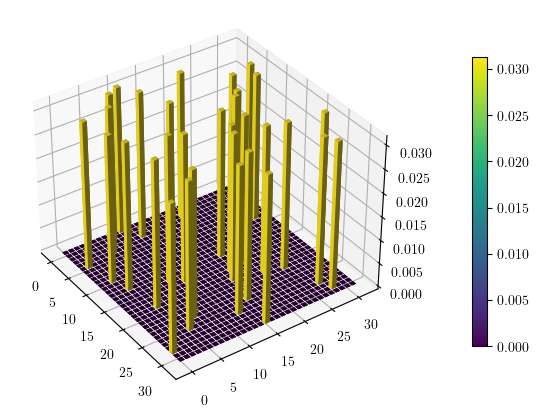
\includegraphics[width=0.6\textwidth]{
    imgs/wigner-standard-2-5-s1.png}
    \caption{Función de Wigner estándar $W$ para el estado
    $\ket{\psi_1}$, el cual pertenece a las MUBs estándar.}
    \label{fig:wigner-standard-2-5-s1}
  \end{figure}
  \begin{figure}[ht]
    \centering
    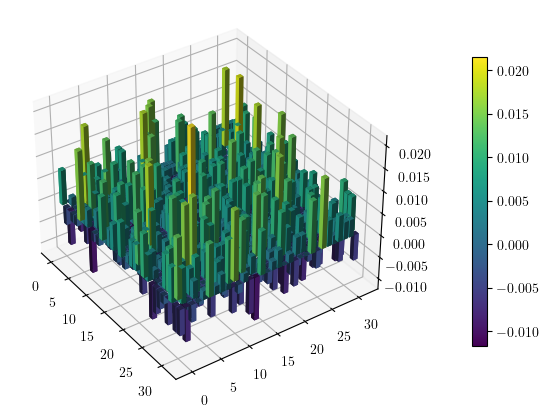
\includegraphics[width=0.6\textwidth]{
    imgs/wigner-kantor-2-5-s1.png}
    \caption{Función de Wigner no-estándar $W^{\mathcal K}$
    para el estado $\ket{\psi_1}$, el cual pertenece a las
    MUBs estándar.}
    \label{fig:wigner-kantor-2-5-s1}
  \end{figure}
  Observemos en la figura (\ref{fig:wigner-standard-2-5-s1})
  que sumando la función de Wigner estándar $W$ sobre la
  recta correspondiente al estado $\ket{\psi_1}$ obtenemos
  el valor de $1$, indicando que no hay incertidumbre. Por
  otro lado, la figura (\ref{fig:wigner-kantor-2-5-s1}) nos
  muestra la función de Wigner no estándar $W^{\mathcal K}$
  del mismo estado $\ket{\psi_1}$. El aparante desorden en
  la gráfica es de esperarse, pues nos indica que el estado
  $\ket{\psi_1}$ \textit{no} es un eigenestado de las
  MUBs de Kantor, un indicador de la inequivalencia entre
  las construcciones. Ahora, las bases correspondientes a
  las rectas horizontales y verticales son las mismas en
  ambas construcciones, así que la suma de ambas funciones
  $W$ y $W^{\mathcal K}$ sobre éstas rectas nos deben dar la
  misma probabilidad, algo que se verifica con cálculo
  directo.

  Similarmente, calculamos las funciones $W$ y $W^{\mathcal
  K}$ pero ahora para el estado $\ket{\psi_2}$ el cual
  pertenece a las MUBs no estándar $\mathcal B^{\mathcal
  K}$, y que no pertenece a la estándar $\mathcal B$.
  \begin{figure}[ht]
    \centering
    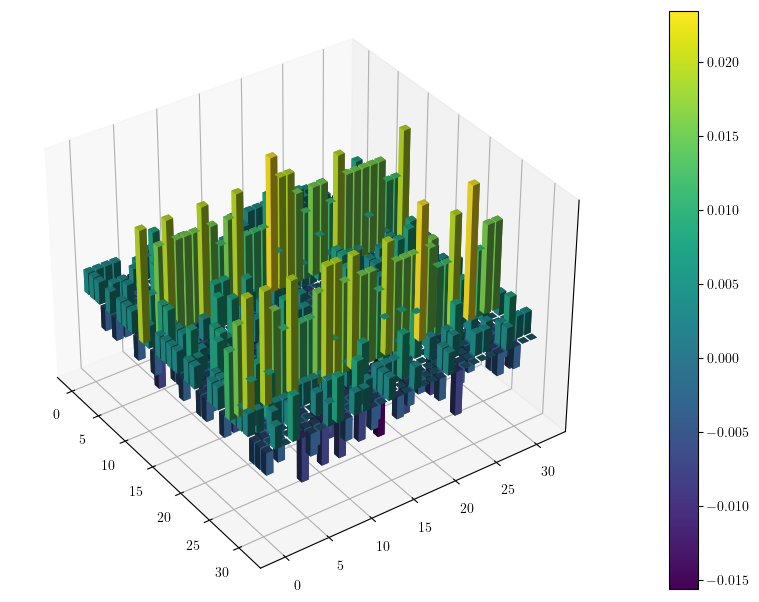
\includegraphics[width=0.6\textwidth]{
    imgs/wigner-standard-2-5-s2.png}
    \caption{Función de Wigner estándar $W$ para el estado
    $\ket{\psi_2}$, el cual pertenece a las MUBs no estándar.}
    \label{fig:wigner-standard-2-5-s2}
  \end{figure}
  \begin{figure}[ht]
    \centering
    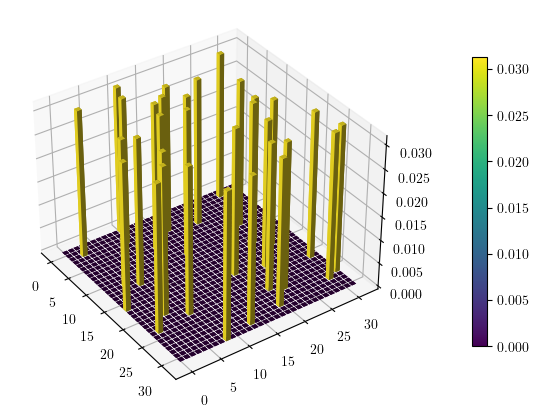
\includegraphics[width=0.6\textwidth]{
    imgs/wigner-kantor-2-5-s2.png}
    \caption{Función de Wigner no estándar para
      $\ket{\psi_2}$.}
    \label{fig:wigner-kantor-2-5-s2}
  \end{figure}
  Como es de esperarse, la figura
  (\ref{fig:wigner-standard-2-5-s2}) nos indica que la
  función de Wigner estándar produce una figura sin mucho.
  Ésto es de esperarse pues las mediciones se hacen con
  bases que no son unitariamente equivalentes a las que se
  usaron para definir la función de Wigner. El mismo estado
  produce una función de Wigner no estándar con mucho más
  orden, en donde se ve claramente que el estado pertenece a
  una de las MUBs. A pesar de las diferencias, en ambos
  casos se preserva la propiedad tomográfica y en estados
  que se comparten en ambas MUBs, las probabilidad obtenidas
  al sumar las funciones de Wigner son iguales.

  Ahora consideremos el estado cuántico $\ket{\psi_3}$. Éste
  estado cuántico es una superposición equitativa de estados
  de la base estándar. La base estándar pertenece a ambos
  conjuntos de MUBs, por lo que no esperaríamos ver mucha
  diferencia. La figura (\ref{fig:wigner-standard-2-5-s3})
  muestra la gráfica de la función de Wigner estándar del
  estado $\ket{\psi_3}$, notemos las dos barras verticales
  que sobre salen. Sumando sobre ellas obtenemos la
  probabilidad de encontrar el sistema en los estados
  $\ket{\alpha^{4}+\alpha^3 + \alpha}$ y $\ket{\alpha+1}$
  respectivamente, en ambos casos la probabilidad es
  $\frac{1}{2}$. Sumando sobre cualquier otra recta vertical
  nos da 0 ya que por definición de $\ket{\psi_3}$ no hay
  probabilidad de que el sistema se encuentre en esos
  eigenestados. Notamos un pico en la primera linea vertical
  que sobresale más que los demas. No podemos concluír mucho
  sobre el significado de ese pico, más de allá del hecho de
  que la probabilidad de transición de $\ket{\psi_3}$ al
  estado correspondente a la recta horizontal que cruza por
  ese punto si coincide con la suma. Como lo esperabamos, la
  gráfica de la función de Wigner no estándar $W^{\mathcal
  K}$ es muy similar, vuelven aparecer dos rectas verticales
  positivas correspondientes a los estados de la
  superposición, como se puede observar en la figura
  (\ref{fig:wigner-kantor-2-5-s3}). Curiosamente, la versión
  no estándar no muestra el pico centralizado que aparece en
  la versión estándar, las barras verticales parecen tener
  alturas distribuidas de una manera más uniforme. El
  cálculo de probabilidades permanece igual. La figura
  (\ref{fig:wigner-2-5-s3-heat}) muestra las gráficas en
  forma de un \textit{mapa de calor} en donde la similutud
  de ambas funciones se aprecia un poco mejor.

  \begin{figure}[ht]
    \centering
    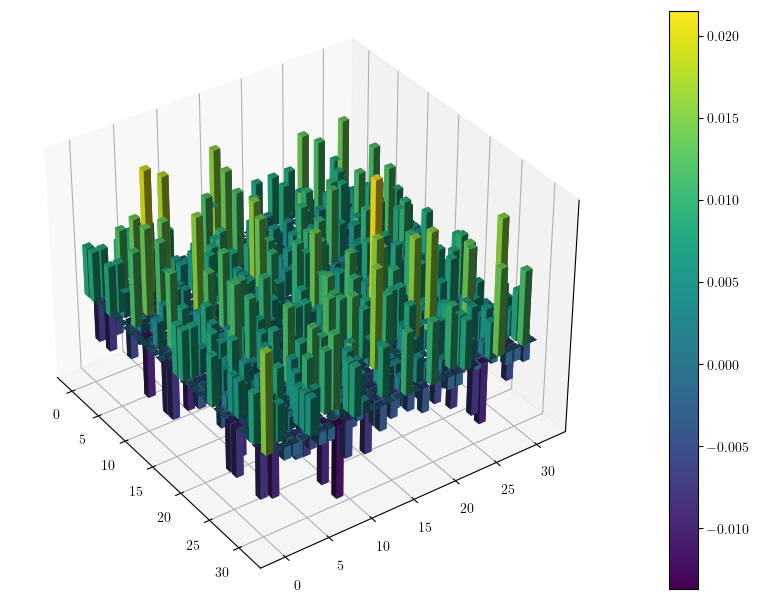
\includegraphics[width=0.6\textwidth]{
    imgs/wigner-standard-2-5-s3.png}
    \caption{ Función de Wigner estándar $W$ del estado en
    superposición.}
    \label{fig:wigner-standard-2-5-s3}
  \end{figure}
  \begin{figure}[ht]
    \centering
    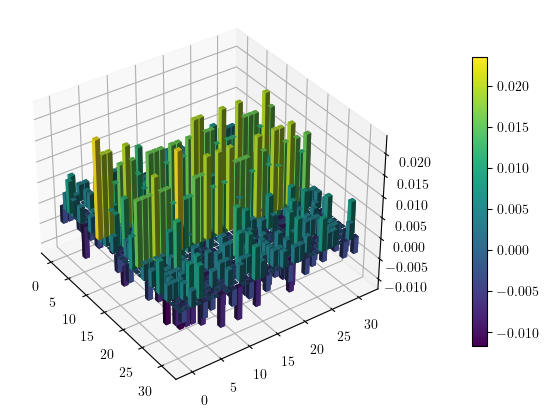
\includegraphics[width=0.6\textwidth]{
    imgs/wigner-kantor-2-5-s3.png}
    \caption{ Función de Wigner no estándar $W^{\mathcal K}$
    del estado en superposición.}
    \label{fig:wigner-kantor-2-5-s3}
  \end{figure}

  \begin{figure}
    \centering
    \subfloat[$W$]{{
        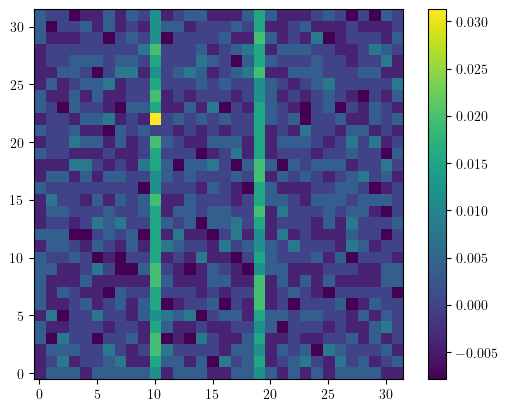
\includegraphics[width=0.415\linewidth]{
        imgs/wigner-standard-2-5-s3-heat.png}
    }}
    \quad
    \subfloat[$W^{\mathcal K}$]{{
        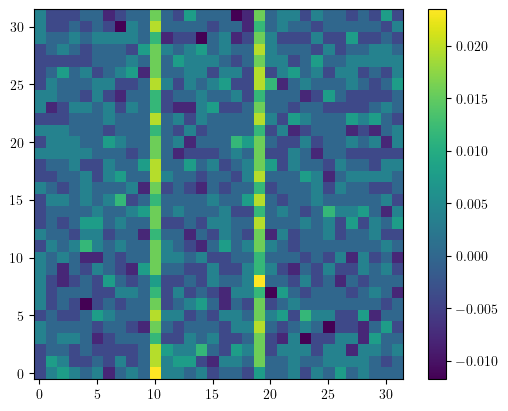
\includegraphics[width=0.415\linewidth]{
        imgs/wigner-kantor-2-5-s3-heat.png}
    }}
    \caption{Comparación de ambas funciones de Wigner para
    el estado $\ket{\psi_3}$.}
    \label{fig:wigner-2-5-s3-heat}
  \end{figure}

  \clearpage
  \begin{example}
    Consideremos el sistema cuántico modelado por tres
    qutrits. En la sección anterior, construímos dos
    conjuntos maximales de MUBs no unitariamente
    equivalentes, así que podremos definir dos funciones de
    Wigner para un estado de interes. Consideramos un
    eigenestado $\ket{\psi}$  de las MUBs estándar.
  \end{example}
  \begin{figure}[ht]
    \centering
    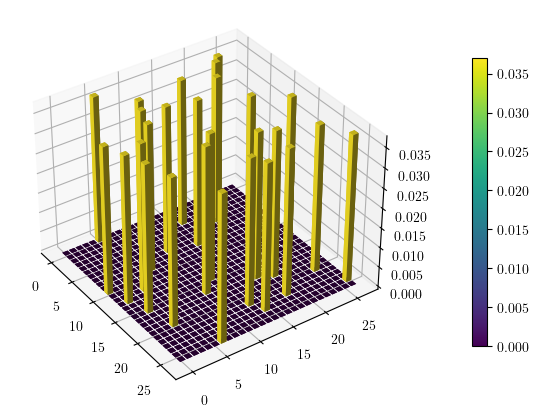
\includegraphics[width=0.6\textwidth]{
    imgs/wigner-standard-3-3-s1.png}
    \caption{Función de Wigner estándar para el estado
    $\ket{\psi}$.}
    \label{fig:wigner-standard-3-3-s1}
  \end{figure}
  \begin{figure}[ht]
    \centering
    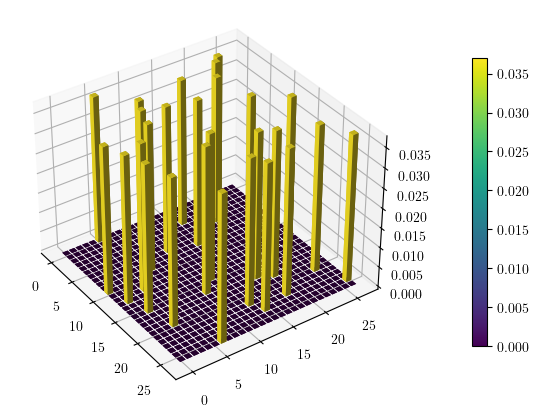
\includegraphics[width=0.6\textwidth]{
    imgs/wigner-standard-3-3-s1.png}
    \caption{Función de Wigner no estándar para el estado
    $\ket{\psi}$.}
    \label{fig:wigner-kantor-3-3-s1}
  \end{figure}
  Las figuras (\ref{fig:wigner-standard-3-3-s1}) y
  (\ref{fig:wigner-kantor-3-3-s1}) muestran la función de
  Wigner estándar $W$ y no estándar $W^{\mathcal K}$ del
  elemento $\ket{\psi}$. \textit{Son idénticas!} Esperabamos
  ver funciones de Wigner muy distintas como sucedió en el
  caso de los cinco qubits, pero como se puede observar, las
  funciones de Wigner no difieren en el caso de tres
  qutrits. Que las MUBs no sean equivalentes bajo ninguna
  transformación unitaria no necesariamente implica que los
  operadores puntuales tampoco lo sean.  El converso es
  claro, pero es probable que la suma de las proyecciones
  de eigenestados de distintas bases \textit{anulen} las
  diferencias. 

  Fue necesario estudiar ésta situación más a fondo. Una
  comparación numérica de las funciones de Wigner apuntó
  hacia la igualdad de los operadores puntuales para ambas
  coberturas simplécticas. Para simplificar la
  investigación, consideremos el operador puntual en el
  origen $A(0,0)$. De la definición de los operadores
  puntuales tenemos que
  \begin{align}
    A(0,0)
    &= \sum_{\lambda \ni (0,0)}^{} Q(\lambda) - I \\
    &= \sum_{m \in \F \cup \{\infty\}}^{} \ket{\lambda_{m,0}}
    \bra{\lambda_{m,0}} - I \\
    &= \ket{e_0}\bra{e_0}
    + \sum_{m \in \F}^{}
    \ket{\lambda_{m,0}}\bra{\lambda_{m,0}} - I,
  \end{align}
  donde $\lambda_{m,0}$ corresponde al rayo con pendiente
  $m$ y $m = \infty$ corresponde con la estría vertical.
  Utilizando la expresión (\ref{eqn:kanat_presemi_mubs})
  tenemos que
  \begin{equation}
    \ket{\lambda_{m,0}}
    = \frac{1}{\sqrt{d}} \sum_{w \in \F}^{}
    \omega^{\tr\left( \frac{1}{2} w(w\circ m) \right) }
    \ket{e_w},
  \end{equation}
  donde $\circ$ es la operación del presemicampo. Notemos
  que la equivalencia del operador puntual se da solo si la
  suma de las proyecciones respecto a la pendiente $m$ es
  igual. Para la cobertura Desarguesiana la operación del
  presemicampo es $w \circ m = wm$ y para la cobertura de
  Albert tenemos que $w \circ m = mw^{9} + m^3 w^3$.
  Utilizando la definición de $\ket{\lambda_{m,0}}$, cada
  proyección se puede expresar como:
  \begin{align}
    \ket{\lambda_{m,0}} \bra{\lambda_{m,0}}
    &= \frac{1}{d} 
    \left(
      \sum_{w \in \F}^{} \omega^{\tr\left( \frac{1}{2}
      w(w\circ m) \right) }
      \ket{e_w}
    \right) 
    \left(
      \sum_{u \in \F}^{} \omega^{-\tr\left( \frac{1}{2}
      u(u\circ m) \right) }
      \bra{e_u}
    \right) \\
    &= \frac{1}{d}
    \sum_{w \in \F}^{} \sum_{u \in \F}^{} 
    \omega^{\tr( \frac{1}{2} w(w\circ m)) - \tr( \frac{1}{2}
    u(u\circ m))} 
    \ket{e_w} \bra{e_u}.
  \end{align}
  Enseguida expresamos el argumento de la traza en términos
  de la definición de las operaciones del presemicampo.
  Primero, para la cobertura Desarguesiana obtenemos la
  expresión:
  \begin{align}
    \tr\left(\frac{1}{2} w(w\circ m)\right)
    - \tr\left(\frac{1}{2} u(u\circ m)\right)
    %&= \tr\left(\frac{1}{2} m w^2\right)
    %- \tr\left(\frac{1}{2} m u^2\right) \\
    &= \tr\left(\frac{1}{2} m \left( w^2-u^2 \right)\right).
  \end{align}
  Similarmente para la cobertura de Albert obtenemos:
  \begin{align}
    \tr\left(\frac{1}{2} w(w\circ m)\right)
    - \tr\left(\frac{1}{2} u(u\circ m)\right)
    %&= \tr\left(\frac{1}{2} w (mw^{9}+m^3w^3)\right)
    %- \tr\left(\frac{1}{2} u (mu^{9}+m^3u^3)\right) \\
    %&= \tr\left( \frac{1}{2} ( 
    %  m w^{10} + m^3 w^{4} - mu^{10} - m^3u^{4}
    %) \right) \\
    &= \tr\left( 
      \frac{1}{2} m \left( w^{10} - u^{10}  
      + m^2 \left( w^{4} - u^{4}\right) \right)
    \right). 
  \end{align}
  Entonces la igualdad de los operadores puntuales es
  equivalente a la igualdad de la siguiente triple suma:
  \begin{equation}
    \sum_{m,w,u \in \F}^{}
    \omega^{\tr(\frac{1}{2} m(w^2-u^2))}
    \ket{e_w}\bra{e_u}
    = 
    \sum_{m,w,u \in \F}^{}
    \omega^{\tr\left(\frac{1}{2} m
    \left(w^{10}-u^{10} +  m^2(w^{4}-u^{4})\right) \right)
    }
    \ket{e_w}\bra{e_u}.
  \end{equation}
  Las proyecciones $\ket{e_w}\bra{e_u}$ en la base
  estándar se representan por matrices con todas sus
  entradas iguales a cero excepto en la entrada indexada por
  los elementos $w$ y $u$. Por lo tanto la igualdad de los
  operadores puntuales en el origen es equivalente a la
  siguiente igualdad:
  \begin{equation}
    \label{eqn:qutrit_weil_sum}
    \sum_{m \in \F}^{}
    \omega^{\tr\left( 
        \frac{1}{2} m \left( w^2 - u^2 \right) 
    \right) }
    =
    \sum_{m \in \F}^{} 
    \omega^{\tr\left( 
        \frac{1}{2} m\left( w^{10}-u^{10} + m^2(w^{4}-u^{4})
        \right) 
    \right) }.
  \end{equation}
  para todo par $u,w \in \F$. A éste tipo de sumas se les
  conoce como sumas de Weil, generalmente se expresan en
  términos de los caracteres del grupo aditivo:
  \begin{equation}
    \sum_{c \in \F}^{} \chi(f(x)),
  \end{equation}
  donde $f \in \F[x]$, (ver la sección de \textit{sumas
  exponenciales} (\ref{subsec:exp_sums}) del apéndice para
  un resumen rápido de los caracteres aditivos de un campo
  finito). Las sumas de Weil generalmente no son fáciles de
  evaluar \cite{lidl1994}.  Usualemente solo podemos obtener
  estimaciones de las cotas superiores e inferiores del
  valor absoluto de la suma. En éste caso particular podemos
  utilizar algunos resultados conocidos para demostrar que
  la igualdad (\ref{eqn:qutrit_weil_sum}) sí se cumple.

  Primero analizamos el lado izquierdo de la ecuación
  (\ref{eqn:qutrit_weil_sum}). Expresamos en términos del
  caracter aditivo no trivial $\chi$ tenemos:
  \begin{equation}
    \sum_{m \in \F}^{} \omega^{\tr\left( \frac{1}{2} \left(
    w^2-u^2\right) m \right) }
    = \sum_{m \in \F}^{} \chi\left( \frac{1}{2} \left(
    w^2-u^2 \right) m \right).
  \end{equation}
  Fijando a $w, u \in \F$, observamos que el argumento
  $\chi$ es lineal siempre y cuando $w^2-u^2 \neq 0$. Si
  $w^2-u^2 = 0$ entonces
  \begin{equation}
    \chi\left( \frac{1}{2} \left(w^2-u^2\right) m \right) 
    = \chi(0)
    = 1.
  \end{equation}
  Por lo tanto la suma de Weil es igual a la cardinalidad de
  la extensión de Galois, $d = |\F| = 27$. Si $w^2-u^2 \neq
  0$, de la linealidad del argumento obtenemos que la suma
  de Weil es igual a 0, por el teorema
  (\ref{thm:lidl_linear_sum}):
  \begin{equation}
    \sum_{m \in \F}^{} \chi(m) = 0.
  \end{equation}
  Se sigue que la suma de Weil tiene dos posibles valores:
  \begin{equation}
    \label{eqn:left_weil_sum}
    \sum_{m \in \F}^{} \omega^{\tr\left(
    \frac{1}{2}(w^2-u^2)m \right) }
    = 
    \begin{cases}
      27 & \text{cuando } w^2-u^2 = 0, \\
      0 & \text{en caso contrario}.
    \end{cases}
  \end{equation}

  Ahora pasemos al lado derecho de la ecuación
  (\ref{eqn:qutrit_weil_sum}). Reescribiendo el argumento de
  la traza y expresando con la notación del caracter aditivo
  obtenemos:
  \begin{equation}
    \sum_{m \in \F}^{} \omega^{\tr\left( \frac{1}{2} m\left(
    w^{10}-u^{10} + m^2(w^{4}-u^{4})\right)  \right) }
    = 
    \sum_{m \in F}^{} \chi\left(
      \frac{1}{2}
      \left( w^{4} - u^{4} \right) m^3
      + \frac{1}{2}
      \left( w^{10} - u^{10} \right) m 
    \right).
  \end{equation}
  El argumento de $\chi$ (sin el factor $1 / 2$) es un
  $p$-polinomio afín de la forma
  \begin{equation}
    f(x) = a_1 x^{p} + a_0 x + a,
  \end{equation}
  donde $p = 3$, $a_1 = w^{4} - u^{4}$,  $a_0 = w^{10} -
  u^{10}$ y $a = 0$. Resulta que podemos evaluar
  directamente a éste tipo de suma de Weil utilizando el
  teorema \ref{thm:lidl_weil_poly}. Sean $b = \frac{1}{2}$ y
  $d = 27$, entonces
  \begin{equation}
    \sum_{m \in \F}^{} \chi\left(
      b \left(
        a_1 m^{3} + a_0 m
      \right)
    \right)
    = 
    \begin{cases}
      \chi_{b}(a) d & \text{cuando } b^3 a_1^3 + b^{3^2}
      a_0^{3^2} = 0 \\
      0 & \text{en otro caso}.
    \end{cases}
  \end{equation}
  Primero notemos que $a = 0$, por lo que $\chi_b(0) = 1$.
  Además el inverso aditivo del dos en característica tres
  es el dos, i.e., $1 / 2 = 2$, por lo tanto la suma de Weil
  es igual a
  \begin{equation}
    \label{eqn:right_weil_sum}
    \sum_{m \in \F}^{} \omega^{\tr\left( \frac{1}{2} m\left(
    w^{10}-u^{10} + m^2(w^{4}-u^{4})\right)  \right) }
    =
    \begin{cases}
      27 & \text{para } \left( w^{4}-u^{4} \right) ^3 +
      2^{6} \left( w^{10} - u^{10} \right) ^{9} = 0, \\
      0 & \text{en otro caso}.
    \end{cases}
  \end{equation}
  De las ecuaciones (\ref{eqn:left_weil_sum}) y
  (\ref{eqn:right_weil_sum}) podemos concluír que ambas
  sumas serán iguales para todo $w, u \in \F$ siempre y
  cuando las ecuaciones
  \begin{equation}
    w^2 - u^2 = 0,
    \quad
    \text{ y }
    \quad
    \left( w^{4}-u^{4} \right)^3
    + 2^{6} \left( w^{10} - u^{10} \right)^{9} = 0,
  \end{equation}
  compartan el \textit{mismo} conjunto de soluciones. Dado
  que estamos trabajando con campos finitos, simplemente
  hemos buscado todas las soluciones de ambas ecuaciones
  para poder compararlas. Para ésto utilizamos el sistema de
  álgebra computacional de \texttt{SageMath} y en particular
  su módulo de campos finitos para encontrarlas.
  \textit{Efectivamente comparten el mismo conjunto de
  soluciones!\footnote{La cardinalidad de éste conjunto de
  soluciones es de 53 elementos $(w,u)$.}} Ésto significa
  que para todo $w, u \in \F$, ambas sumas de la ecuación
  (\ref{eqn:qutrit_weil_sum}) nos dan el mismo valor, ya sea
  $0$ ó $27$. Ésto a su vez significa que los operadores
  puntuales en el origen para ambas coberturas simplécticas
  son iguales. Un cálculo computacional similar nos muestra
  que el resto de los operadores puntuales también lo son.
  Como consecuencia, obtenemos la misma función de Wigner
  para la construcción estándar y no estándar en el caso de
  los tres qutrits, respecto a la cobertura de Albert. Éste
  ejemplo nos indica que la no equivalencia de las MUBs
  \textit{no} es suficiente para garantizar la desigualdad
  de las funciones de Wigner estándar y no estándar.

  Wootters y Gibbons propusieron una manera de estudiar la
  equivalencia de funciones de Wigner discretas bajo
  relaciones de equivalencia dadas por transformaciones
  unitarias de las mallas cuánticas.
  \begin{definition}
    Decimos que dos mallas cuánticas son equivalentes si
    solo difieren por una transformación unitaria, es decir,
    dos mallas cuánticas $Q$ y $Q'$ son iguales si existe
    una transformación unitaria $U$ tal que
    \begin{equation}
      Q'(\lambda)
      = U Q(\lambda) U^{*},
    \end{equation}
    para toda curva $\lambda$ del espacio de fase discreto.
  \end{definition}
  %Utilizando ésta definición, Wootters prueba mediante un
  %argumento de conteo, que toda malla cuántica es equivalente
  %si y solo si el plano afín difiere por una traslación en
  %el espacio de fase discreto.
  Por un lado es fácil ver que si $Q$ y $Q'$ son
  unitariamente equivalentes, entonces los operadores
  puntuales $A(\alpha)$ y $A'(\alpha)$ también lo son, ya
  que
  \begin{align}
    A'(\alpha)
    &= \sum_{\lambda \ni \alpha}^{} Q'(\lambda) - I \\
    &= \sum_{\lambda \ni \alpha}^{} U Q(\lambda) U^{*} - I
    \\
    &= U \left( 
      \sum_{\lambda \ni \alpha}^{} Q(\lambda) - I
    \right) U^{*} \\
    &= U A(\alpha) U^{*}.
  \end{align}
  ¿La proposición conversa también se cumple? Si los
  operadores puntuales son unitariamente equivalentes, ¿ésto
  implica que las mallas también lo son? Dicho de otra
  manera, si utilizamos MUBs no equivalentes, ¿los
  operadores puntuales tampoco serán equivalentes?  Nuestro
  ejemplo de los tres qutrits con las coberturas
  Desarguesiana y de Albert es un contra ejemplo de la
  proposición conversa, ya que la identidad es una
  transformación unitaria. En otras palabras, incluso cuando
  no existe una transformación unitaria entre dos mallas
  cuánticas, los operadores puntuales pueden ser
  equivalentes. Por lo tanto el método de Wootters para
  clasificar funciones de Wigner equivalentes parece no ser
  apropiado cuando uno desea comparar la función de Wigner.
  Parece ser necesario estudiar que propiedades adicionales
  debe tener una malla cuántica o el espacio de fase
  discreto en particular, para poder determinar cuando una
  función de Wigner es unitariamente distinta a otra. 

  El hecho de que ésto no sucede en el ejemplo de los cinco
  qubits puede ser consecuencia de la cobertura particular
  que usamos para la construcción no estándar, ó,
  posiblemente es otra consecuencia interesante de la
  característica par. 

  \clearpage
  \section{Discusión}

  Hemos construido dos versiones de funciones de Wigner para
  sistemas de dimensión finita. El método de construcción se
  basa en la metodología de Wootters y Gibbons, en donde le
  asignamos una estructura cuántica al espacio de fase
  discreto. La estructura cuántica corresponde a un conjunto
  maximal de bases mutuamente insesgadas, las cuales dotan a
  la función de Wigner las propiedades análogas al caso
  continuo, en particular la propiedad tomográfica.
  Ésta propiedad nos permite recuperar el operador de
  densidad a partir de su función de Wigner. Dada la
  libertad en la asignación de la estructura cuántica al
  espacio de fase discreto, pudimos construir una versión no
  estándar utilizando MUBs que no son unitariamente
  equivalentes a las de Wootters. A pesar de ésto, no
  logramos concluir sobre la inequivalencia entre las
  funciones de Wigner producidas por ambas construcciones,
  ya que la no equivalencia de las MUBs no es una condición
  suficiente para producir funciones de Wigner discretas
  distintas, como nos muestra el ejemplo de los tres
  qutrits.

  Otro aspecto de éste método de construcción que es victima
  de la arbitrariedad, es que la gráfica de una función de
  Wigner depende del orden elegido del campo finito
  utilizado para armar el espacio de fase. Evidentemente no
  hay un ordenamiento predilecto, ya que los campos finitos
  no son ordenados.  Durante todo el trabajo hemos optado
  por utilizar el ordenamiento por potencias del generado de
  la extensión de Galois, pero se ha observado que distintos
  ordenamientos producen gráficas con distintas cualidades,
  unas más ordenadas que otras. Como trabajo futuro sería
  interesante estudiar los efectos del orden elegido en
  cuanto alguna medida del orden o aleatoriedad de la
  gráfica de la función de Wigner, y estudiar si ésto tiene
  consecuencias en las interpretaciones físicas.

  Por otro lado, la metodología de Wootters revela de manera
  directa la relación que existe entre estructuras
  geométricas finitas y algunas particularidades de los
  sistemas cuánticos discretos. Como hemos mencionado
  anteriormente, aun es un problema abierto el encontrar la
  cantidad máxima de bases mutuamente insesgados para
  sistemas de dimensión compuesta que no son potencias de
  primos. De la misma manera existen problemas abiertos
  análogos en el álgebra combinatoria \cite{kantor2003}, en
  la teoría de códigos \cite{kantor1982} y en la teoría de
  las álgebras de Lie \cite{ivanov1987, kantor1996,
  boykin2005}, entre otros, que parece indicar una relación
  más profunda. Es posible que hallazgos y avances en
  algunas de éstas áreas nos provee la solución al problema
  de las MUBs o vice-versa. Si los sistemas de dimensión que
  son potencias de primos son los únicos de los cuales
  podemos obtener la cantidad máxima de MUBs, ¿qué nos dice
  ésto en cuestión de la tomografía cuántica y en la
  cuestión de la medición de estados cuánticos?

  En un aspecto más práctico, el hecho de que podemos
  obtener MUBs que no son unitariamente equivalentes a las
  `clasicas', nos da la posibilidad de encontrar otros
  esquemas de factorización que pudieran resultar útiles
  para ciertos problemas físicos. Ésto es otra dirección
  interesante que nos gustaría investigar posteriormente.
  También recordamos que unas de las motivaciones
  principales de éste trabajo fueron los resultados
  relativamente recientes de Gross \cite{gross2006} entre
  otros, que relacionan la positividad de una versión
  particular de la función de Wigner discreta con estados
  Gaussianos, entre ellos los estabilizadores, de los cuales
  se ha probado que son simulables de manera clásica. Una
  investigación futura podría involucrar la busqueda de
  estados no estabilizadores con funciones de Wigner no
  estándar no negativa, algo que contrastaría con los
  resultados previos.

  \newpage
  \appendix
  \chapter{Apéndices}

  \section{La mecánica clásica y el espacio de fase}

  El concepto del espacio de fase es una herramienta de la
  mecánica clásica, la cual describe la evolución temporal
  de un sistema físico. Dicho de una manera muy sencilla, la
  mecánica clásica estudia partículas y sus trayectorias,
  las cuales se rigen de acuerdo a las leyes de Newton.  Se
  considera que la partícula se `mueve' en un espacio
  euclideano, es decir, su \textit{posición} está dado por
  $x = (x_1,\ldots,x_n) \in \R^{n}$. El
  \textit{momentum} es una cantidad dada por $p_j = m \dot
  x_j$, donde $\dot x$ es la derivada respecto al
  tiempo de la posición, es decir, la velocidad de la
  partícula, y $m$ es la \textit{masa} de la partícula. Las
  cantidades que uno desea medir de nuestro sistema físico
  se les llama \textit{observables}, y en la mecánica
  clásica, son las funciones continuas que tienen como
  argumentos las cantidades $x,p$ y $m$. Ejemplos
  de ellos son el momentum, la energía cinética, la energía
  potencial, etc. La función de energía más usual es la que
  está dada como la suma de la \textit{energía cinética} y
  \textit{energía potencial}:
  \begin{equation}
    H(x,p)
    = \frac{1}{2m} \sum_{j=1}^{n} p_j^2 + V(x).
  \end{equation}
  A la energía del sistema se le conoce como el
  \textit{Hamiltoniano}.  Utilizando ésta función de
  energía, la ley de Newton nos brinda las ecuaciones de
  movimiento de la partícula en cuestión:
  \begin{equation}
    \frac{dx_j}{dt}
    = \frac{\partial H}{\partial p_j},
    \quad
    \frac{dp_j}{dt}
    = -\frac{\partial H}{\partial x_j}.
  \end{equation}
  Expresada como un sistema de ecuaciones diferenciales, a
  la ley de Newton se le conoce como las \textit{ecuaciones
  de Hamilton}. Con ésto, es natural representar el estado
  del sistema clásico considerando el par $(x,p) \in
  \R^{2n}$. Al espacio $\R^{2n}$ se le conoce como el
  \textit{espacio de fase}. A las soluciones de las
  ecuaciones de Hamilton se les conoce como
  \textit{trayectorias}, y son curvas que viven en el
  espacio de fase.
  \begin{definition}
    El espacio de fase de una partícula que se mueve en
    $\R^{n}$ es $\R^{2n}$, considerado como el conjunto de
    las $(2n)$-tuplas de la forma
    \[
      \left(
        x_1, \ldots, x_n, p_1, \ldots, p_n
      \right),
    \] 
    donde $x_j$ y $p_j$ son elementos de $\R$.
  \end{definition}

  Cabe mencionar que el tratado moderno de la mecánica
  clásica está fundamentado en la geometría diferencial de
  las variedades simplécticas
  \cite{mcinerneyFirstStepsDifferential2013}, en donde el
  espacio de fase se define como el espacio cotangente del
  espacio de configuraciones $T^{*} \R_x \cong \R_x \times
  \R_p$, donde el espacio de configuraciones  $\R_x$ es el
  espacio de posición y el $\R_p$ es el espacio del
  momentum.  Para nuestros objetivos basta con desginar el
  espacio de fase como el espacio $\R^{2n}$.

  Notemos que por el momento no ha surgido ninguna
  interpretación probabilística en la mecánica clásica, pues
  es una teoría determinística. Dado que la teoría cuántica
  es probabilística, es natural preguntarnos ¿qué
  características de la mecánica clásica serían deseables en
  la teoría cuántica? y ¿qué beneficios habría en hacer un
  vínculo entre la mecánica clásica y la cuántica?
  \cite{schroeckQuantumMechanicsPhase1996}, especialmente
  cuando sabemos que la teoría cuántica (y sus derivados) es
  nuestra teoría más precisa. Un esfuerzo por vincular las
  descripciones clásicas y cuánticas del mundo es la
  representación de Wigner-Weyl-Moyal de la mecánica
  cuántica.  Ésta es una formulación que intenta usar la
  noción del espacio de fase en la dinámica cuántica y la
  idea básica es la construcción de
  \textit{cuasi-distribuciones} real-valuadas que
  representan a los sistemas cuánticos.

  \section{Resumen de Folland}

  Para Folland, la transformación de Wigner de dos funciones
  $f$ y $g$ es la transformación de Fourier de la
  transformación de Fourier-Wigner:
  \[
    W(f,g)(\xi, \eta)
    = \int_{\R^{2n}} e^{-2\pi i (\xi q + \eta p} V(f,g)(q,x)
    \, dp \, dq.
  \] 
  Donde
  \[
    V(f,g)(q,p)
    = \int e^{2\pi i q y} f(y + \frac{1}{2}p)\overline{g(y -
    \frac{1}{2}p)} \, dy.
  \] 
  Así que
  \[
    W(f,g)(\xi, \eta) = \int e^{-2\pi i \eta p }
    f(x+\frac{1}{2}p)\overline{g(y-\frac{1}{2}p)} \, dp.
  \] 

  Folland muestra que $W$ mapea $\Sz(\R^{n}) \times
  \Sz(\R^{n})$ a $\Sz(\R^{2n})$ y se puede extender al caso
  de las distribuciones templadas.

\section{Anillos y campos}

  Si intentamos definir el espacio de fase discreto sobre un
  anillo como $\Z_4$ tendremos problemas a la hora de
  definir las rectas. Por ejemplo si consideramos la recta
  \[
    x + 2p = 0,
  \]
  que tiene como solución al conjunto de puntos
  \[
    \{(0,0), (2,1), (0,2), (2,3)\}.
  \] 
  Ahora, la recta 
  \[
    x = 0,
  \] 
  tiene como solución al conjunto
  \[
    \{(0,0), (0,1), (0,2), (0,3)\}.
  \] 
  Notemos que los dos conjuntos tiene una intersección con
  más de un elemento, algo que contradice nuestra noción
  geoemétrica de una linea en el espacio.

  Sea $\F_N$ un campo de $N$ elementos donde $N = r^{k}$ es
  una potencia de un número primo $r$. El primo $p$ se
  conoce como la característica de $\F_N$ y se define como
  el número entero más pequeño tal que
  \[
    1 + 1 + \ldots + 1 = 0.
  \] 
  $\F_r$ es simplemente $\Z_r$ pero $\F_N$ no es $\Z_N$.
  Para construir a $\F_N$ requerimos de un polinomio $f(x)$ 
  de grado $k$ que es irreducible en $\F_r$. Si $\alpha$ es
  una raíz de $f(x)$, el campo que obtenemos al adjuntar
  $\alpha$ a $\F_r$ es
  \[
    \F_N
    = \F_r(\alpha) \cong \F_r[x] / \langle f(x) \rangle.
  \] 
  \begin{example}
    Consideremos el anillo $\Z_4$ y el polinomio $f(x) = x^2
    + x + 1$. El campo de Galois es
    \[
      \F_2[x] / (x^2 + x + 1)
      \cong \F_2(\alpha)
      = \{0, 1, \alpha, \alpha + 1\},
    \] 
    donde $\alpha^2 + \alpha + 1 = 0$. En el campo $\F_2 =
    {0,1}$ no hay soluciones al polinomio $f(x)$ y definimos
    su solución como $\alpha$. Todo elemento de
    $\F_2(\alpha)$ tiene la forma $a_1 \alpha + a_0$, donde
    $a_j \in \F_2$, por lo tanto $\{1, \alpha\}$ es una base
    de espacio vectorial de $\F_4$ sobre $\F_2$.
  \end{example}

  El mapeo $\sigma : \alpha \to \alpha^r$ donde $\alpha \in
  \F_N$ es un automorfismo lineal de $\F_N$ llamado el
  \textit{automorfismo de Frobenius} que nos da los
  conjugados de Galois. Elementos del campo primo son
  invariantes bajo $\sigma$. Definimos la operación de traza
  de un elemento $\alpha \in \F_N$ (distinta a la traza de
  un operador lineal) como:
  \[
    \tr(\alpha) 
    = \alpha + \alpha^{r} + \alpha^{r^2} + \ldots +
    \alpha^{r^{k-1}}
    = \sum_{m=0}^{k-1} \sigma^{m}(\alpha).
  \] 
  La operación $\tr$ mapea a todo elemento del campo finito
  a un elemento del campo primo $\tr : \F_N \to \F_r$. Para
  cualquier base $E = \{e_0,e_1,\ldots,e_{N-1}\}$, existe
  una única base de campo $\tilde E = \{\tilde
  e_0,\ldots,\tilde e_{N-1}\}$ tal que $\tr(\tilde e_j e_k)
  = \delta_{jk}$. La base $\tilde E$ se llama la base dual a
  $E$. Podemos utilizar la base dual para encontrar la
  expansión única en coeficientes respecto a la base $E$ 
  para cualquier elemento $x$ del campo. Para obtener el
  componente $x_s$ del elemento $x$, hacemos
  \[
    \tr(x \tilde e_s)
    = \sum_{r}^{k} x_r \tr(e_r \tilde e_s)
    = x_s.
  \]

  \section{Klappenecker, Godsil, Roy}

  \subsection{Característica impar}

  Consideremos un espacio de Hilbert de dimensión $d =
  p^{n}$ donde $p$ es un primo impar, y sea $\{\ket{u}\}$ la
  base estándar para el espacio $\C^{d}$ indexado por los
  elementos de la extensión de Galois $\mathbb F_{d} =
  \GF(p,n)$. Dado un $a \in \mathbb F_d$, definamos los
  operadores
  \begin{align}
    X(a) &: \ket u \mapsto \ket{u+a} \\
    Z(a) &: \ket u \mapsto \omega^{\tr(au)} \ket{u}.
  \end{align}
  Notemos que son los operadores de desplazamiento básicos
  que definimos anteriormente en la metodología de Wootters
  y Gibbons, pero ésta vez las operaciones dentro de los
  kets y en las potencias de la raíz primitiva son las del
  campo finito y no solo operaciones módulo $p$. Recordamos
  que la base estándar es un conjunto completo de
  eigenvectores de $Z(a)$. Además la base `Fourier
  conjugada'
  \[
    \ket{\tilde u}
    = \sum_{v \in \mathbb F_d}^{} \omega^{\tr(uv)} \ket{v},
    \quad u \in \mathbb F_d,
  \] 
  es un conjunto completo de eigenvectores del operador
  $X(a)$. De nuevo definamos a los operadores de
  desplazamiento generales como
  \[
    D(a,b) = X(a)Z(b).
  \] 
  Cada operador de desplazamiento es unitario y monomial.
  Bandyopadhyay et al particionan dichas matrices en
  conjuntos mutuamente conmutativos y demuestra que los
  eigenvectores simultáneaos de cada conjunto forman bases
  mutuamente insesgadas. La siguiente proposición nos dice
  como construir a esos eigenvectores.
  \begin{proposition}
    Sea $D(a,b)$ un operador de desplazamiento donde $a,b
    \in \mathbb F_d$. Si $c$ y $n$ son elementos del campo
    tales que $c = \frac{b}{2a}$, entonces el vector
    \begin{equation}
      \ket{a,b; n}
      = \sum_{x \in \mathbb F_d}^{} \omega^{\tr(cx^2+2nx)}
      \ket{u},
    \end{equation}
    es un eigenvector de $D(a,b)$.
  \end{proposition}
  \begin{proof}
    .
  \end{proof}

  \subsection{Característica par}

  El caso donde el campo primo es de característica par es
  un poco más complicado. ¿Por qué? En éste caso es
  necesario hacer operaciones en un \textit{anillo} de
  Galois. Sea $\Z_4$ el anillo de los enteros módulo 4.
  Decimos que un polinomio $h(x) \in \Z_4[x]$ es un
  \textit{primitivo básico} si y solo si su imágen en
  \[
    \Z_4[x] / \langle 2 \rangle
    \cong
    \Z_2[x]
  \] 
  bajo el mapeo canónico es un polinomio primitivo en
  $\Z_2[x]$. Sea $h(x)$ un polinomio primitivo básico mónico
  de grado $n$, entonces el anillo
  \begin{equation}
    GR(4,n)
    = \Z_4[x] / \langle h(x) \rangle    
  \end{equation}
  se cono como el anillo de Galois de grado $n$ sobre
  $\Z_4$.
  Sea $\xi$ el elemento primitivo de orden $2^{n}-1$ del
  anillo y consideremos el conjunto Teichmüller
  \[
    T_n
    = \{0,1,\xi,\ldots,\xi^{2n-2}\},
  \] 
  del anillo. Klappenecker [CITE] nos menciona que todo
  elemento $r \in GR(4,n)$ puede ser expresado de manera
  única en la forma $r = a + 2b$ donde $a,b \in T_n$. Con
  ésta caracterización de los elementos del anillo en
  términos de los elementos del Teichmüller podemos definir
  el automorfismo de Frobenius (ver apéndice ()) $\sigma :
  GR(4,n) \to \Z_4$ definido como
  \[
    \sigma(a+2b)
    = a^2+2b^2.
  \] 
  Con ésto definamos a la traza del anillo de Galois $\tr :
  GR(4,n) \to \Z_4$ utilizando el mapa de Frobenius:
  \[
    \tr(r)
    = \sum_{k=0}^{n-1} \sigma^{k}(r).
  \] 
  Con éstos acordes Klappenecker construye las siguientes
  bases mutuamente insesgadas.
  \begin{proposition}
    Sea $GR(4,n)$ el anillo de Galois de $4^{n}$ elementos y
    $T_n$ su Teichmüller. Entonces el conjunto de vectores
    definidos como
    \begin{equation}
      \ket{a; b}
      = 2^{-n / 2} \left(
        \eta^{\tr\left( ax + 2bx \right)}
      \right)_{x \in T_n},
    \end{equation}
    donde $\eta = e^{2\pi i / 4}$, son bases mutuamente
    insesgadas del espacio $\C^{2^{n}}$.
  \end{proposition}

  Godsil y Roy definen las matrices de Pauli para $a, u \in
  T$ como
  \begin{align}
    X(a) &: \ket u \mapsto \ket{u+a+2 \sqrt{ua}} \\
    Z(a) &: \ket u \mapsto (-1)^{\tr(au)} \ket{u}
    = i^{\tr(2au)}\ket u.
  \end{align}
  \begin{proposition}
    Si $c,d \in T$, los vectores
    \begin{equation}
      \ket{c,d}
      = \sum_{x \in T}^{} i^{\tr(cx^2+2dx)} \ket x,
    \end{equation}
    son eigenvectores de los operadores de desplazamiento
    $D(a,b)$, donde $a,b \in T$.
  \end{proposition}

  \section{Campos y anillos de Galois}

  \subsection{Extensiones de campo}

  Como hemos visto, la estructura algebráica del campo
  finito es necesaria para poder construir una función de
  Wigner discreta con todas las propiedades deseables. La
  artimética $d$-modular no es suficiente ya que no se
  preservan ciertas propiedades importantes de una geometría
  finita. Los campos $\Z_p$ donde $p$ es un número primo son
  los más sencillos de manejar porque las operaciones se
  hacen módulo $p$, pero ésto se vuelve inpráctico porque no
  todo sistema cuántico puede ser modelado por un espacio de
  Hilbert de dimensión prima. El concepto de una
  \textit{extensión de campos} nos permite augmentar el
  campo $\Z_p$ a un campo finito de orden $p^{n}$. A la
  extensión de campo se le dice \textit{extensión de Galois}
  y son de característica $p$.

  Consideremos al anillo de polinomios $\Z_p[x]$ con
  coeficientes en el campo primo $\Z_p$. Sea $p(x)$ un
  polynomio mónico irreducible de grado $n$:
  \begin{equation}
    p(x)
    = c_0 + c_1 x + \cdots + c_{n-1} x^{n-1} + x^{n},
    \quad c_n \in \Z_p.
  \end{equation}
  El cociente $\Z_p[x] / p(x)$ es un representación del
  campo de Galois $\GF(p^{n})$. Distintos polinomios
  irreducibles del mismo grado nos brinda campos finitos
  isomorfos. Las operaciones de la extensión de campo son
  las operaciones de suma y multiplicación usuales, módulo
  el polinomio $p(x)$. Es importante notar que un elemento
  $\alpha \in \GF(p^{n})$ se puede ver como un vector
  $(\alpha_0, \alpha_1, \ldots, \alpha_{n-1})$ en
  $(\Z_p)^{n}$, utilizando la base
  $\{1,\omega,\ldots,\omega^{n-1}\}$ donde $\omega$ es una
  raíz del polinomio irreducible. De ésta manera la adición
  en la extensión se reduce a la adición usual del espacio
  vectorial $(\Z_p)^{n}$. Enseguida definimos algunos
  conceptos necesarios para trabajar con el espacio de fase
  discreto y para desarrollar la metodología de Wootters
  para la construcción de la función de Wigner.

  \begin{definition}
    Sea $\GF(p^{n})$ un campo de Galois, definimos la
    transformación de Frobenius como
    \begin{equation}
      \sigma(\alpha) = \alpha^{p};
      \quad
      \sigma^{n} = 1.
    \end{equation}
    Dicha transformación define un automorfismo en
    $\GF(p^{n})$ y produce los \textit{conjugados de
    Galois}.
  \end{definition}

  \begin{definition}
    La traza de un elemento $\alpha \in \GF(p^{n})$ es la
    suma de todos sus conjugados, y es un elemento del campo
    primo $\Z_p$:
    \begin{equation}
      \tr(\alpha)
      = \tr_{n / 1}(\alpha)
      = \alpha + \alpha^{p} + \alpha^{p^2} + \cdots +
      \alpha^{p^{n-1}}.
    \end{equation}
  \end{definition}
  La traza así definida es la traza \textit{respecto} a la
  extensión de $\Z_p$ a $\GF(p^{n})$. La traza es lineal
  respecto a la suma en los elementos de la extensión, y si
  $\alpha \in \Z_p$ entonces $\tr(\alpha\beta) =
  \alpha\tr(\beta)$ para todo $\beta \in \GF(p^{n})$.

  \subsection{Bases de una extensión de Galois}

  . . .

  Para construir la base dual y para el cálculo de la traza de
  los elementos de la extensión, resulta ventajoso definir
  la siguiente matriz con elementos en el campo primo.

  \begin{proposition}
    Sean $g,G$ las siguientes matrices simétricas e
    invertibles $n \times n$ con elementos en $\Z_p$:
    \begin{equation}
      g_{ij}
      = \tr(\omega^{i+j});
      \quad
      G = g^{-1},
      \quad
      i,j = 0,\ldots,n-1.
    \end{equation}
    El conjunto de elementos $\{E_0,E_1,\ldots,E_{n-1}\}$ 
    definido como
    \begin{equation}
      E_i = \sum_{j}^{} G_{ij} \omega^{j},
    \end{equation}
    es una base dual a
    $\{1,\omega,\omega^2,\ldots,\omega^{n-1}\}$.
  \end{proposition}

  Con lo anterior, podemos calcular los
  componentes de cualquier elemento $\alpha$ de la extensión
  de campos, en términos de la base o de su dual:
  \begin{align}
    \alpha_i
    &= \tr(\alpha E E_i);
    \quad
    \overline{\alpha}_i
    = \tr(\alpha \omega^{i}) \\
    \alpha_i 
    &= \sum_{j}^{} G_{ij} \overline{\alpha}_j;
    \quad
    \overline{\alpha}_i
    = \sum_{j}^{} g_{ij} \alpha_j.
  \end{align} 

  \subsection{Sistemas compuestos y factorización tensorial}

  Sabemos que una extensión de Galois $\GF(p^{n})$ se puede
  ver como un espacio vectorial sobre el campo primo $\Z_p$
  respecto a la adición del campo. Pero también tiene más
  estructra, como la multiplicación y las transformaciones
  de Frobenius. Por ésto, Vourdas [CITE] nota que
  representar un sistema cuántico con una extensión de
  Galois de grado $n$ no es lo mismo que representarlo con
  una suma directa del campo primo. 

  Sea $\ket{\alpha}$ un base ortonormal de un espacio de
  Hilbert $\H$ de dimensión $p^{n}$, indexada por los
  elementos de una extensión de Galois. Además sea $\H_p$ un
  espacio de dimensión $p$ y $\ket{k}$ un base ortonormal de
  $\H_p$ indexado por los elementos del campo primo $\Z_p$.
  Utilizando la base natural de la extensión de campo,
  podemos expresar a cualquier elemento $\alpha \in
  \GF(p^{n})$ como $\alpha = \sum_{i}^{} \alpha_i \omega^{i}
  $, ésto nos da un mapeo biyectivo:
  \begin{equation}
    \label{eqn:extension_field_map}
    \alpha \mapsto (\alpha_0,\ldots,\alpha_{n-1}),
  \end{equation} 
  lo cual induce una correspondencia entre los elementos de
  la base de $\H$ y $\H_p$:
  \begin{equation}
    \ket{\alpha}
    = \ket{\alpha_0 + \alpha_1 \omega + \ldots +
      \alpha_{n-1}\omega^{n-1}}
    \mapsto \ket{\alpha_0} \otimes \ket{\alpha_1} \otimes
    \cdots \otimes \ket{\alpha_{n-1}},
  \end{equation}
  la cual a su vez nos da una correspondencia entre los
  espacios de Hilbert $\H$ y $\H_p \otimes \cdots \otimes
  \H_p$. Notemos que la correspondencia depende de la
  elección de base del campo, por lo que la construcción de
  otros objetos por medio del producto tensorial también
  serán afectados. Por ejemplo los operadores de
  desplazamiento que actuán sobre el espacio de Hilbert de
  dimensión $p^{n}$ pueden ser expresados en términos de
  productos tensoriales de operadores de desplazamiento en
  los subsistemas. El mapeo(\ref{eqn:extension_field_map})
  nos permite hacer ésto como:
  \begin{equation}
    D(\alpha,\beta)
    = D(\alpha_0, \beta_0) \otimes \cdots \otimes
    D(\alpha_{n-1}, \beta_{n-1}),
  \end{equation}
  donde $\alpha_i$ son los componentes de $\alpha$ en la
  base elegida, y $\beta_i$ son los componentes respecto a
  la base dual, y los operadores $D(\alpha_i,\beta_i)$ son
  los operadores de desplazamiento actuando sobre los
  subsistemas $\H_p$.

  Klimov. . .


  \newpage
  \printbibliography

\end{document}
